
%%%%%%%%%%%%%%%%%%%%%%%%%%%%%%%%%%%%%%%%%%%%%%%%%%%%%%%%%%%%%%%%%%%%%%%%%%%%%
%
% Package pgfplots.sty documentation.
%
% Copyright 2007/2008 by Christian Feuersaenger.
%
% This program is free software: you can redistribute it and/or modify
% it under the terms of the GNU General Public License as published by
% the Free Software Foundation, either version 3 of the License, or
% (at your option) any later version.
%
% This program is distributed in the hope that it will be useful,
% but WITHOUT ANY WARRANTY; without even the implied warranty of
% MERCHANTABILITY or FITNESS FOR A PARTICULAR PURPOSE.  See the
% GNU General Public License for more details.
%
% You should have received a copy of the GNU General Public License
% along with this program.  If not, see <http://www.gnu.org/licenses/>.
%
%
%%%%%%%%%%%%%%%%%%%%%%%%%%%%%%%%%%%%%%%%%%%%%%%%%%%%%%%%%%%%%%%%%%%%%%%%%%%%%
% SEE pgfplots-macros.tex as well!
%\pdfminorversion=5 % to allow compression
%\pdfobjcompresslevel=2
\documentclass[a4paper,openany]{book}

\let\bookmaketitle=\maketitle

% -----------------------------------
% this here is from ltxdoc:
\usepackage{doc}
\AtBeginDocument{\MakeShortVerb{\|}}
%\setlength{\textwidth}{355pt}
%\addtolength\marginparwidth{30pt}
%\addtolength\oddsidemargin{20pt}
%\addtolength\evensidemargin{20pt}
\def\cmd#1{\cs{\expandafter\cmd@to@cs\string#1}}
\def\cmd@to@cs#1#2{\char\number`#2\relax}
\DeclareRobustCommand\cs[1]{\texttt{\char`\\#1}}
\providecommand\marg[1]{%
  {\ttfamily\char`\{}\meta{#1}{\ttfamily\char`\}}}
\providecommand\oarg[1]{%
  {\ttfamily[}\meta{#1}{\ttfamily]}}
\providecommand\parg[1]{%
  {\ttfamily(}\meta{#1}{\ttfamily)}}
\raggedbottom

% -----------------------------------

%%%%%%%%%%%%%%%%%%%%%%%%%%%%%%%%%%%%%%%%%%%%%%%%%%%%%%%%%%%%%%%%%%%%%%%%%%%%%
%
% Package pgfplots.sty documentation.
%
% Copyright 2007/2008 by Christian Feuersaenger.
%
% This program is free software: you can redistribute it and/or modify
% it under the terms of the GNU General Public License as published by
% the Free Software Foundation, either version 3 of the License, or
% (at your option) any later version.
%
% This program is distributed in the hope that it will be useful,
% but WITHOUT ANY WARRANTY; without even the implied warranty of
% MERCHANTABILITY or FITNESS FOR A PARTICULAR PURPOSE.  See the
% GNU General Public License for more details.
%
% You should have received a copy of the GNU General Public License
% along with this program.  If not, see <http://www.gnu.org/licenses/>.
%
%
%%%%%%%%%%%%%%%%%%%%%%%%%%%%%%%%%%%%%%%%%%%%%%%%%%%%%%%%%%%%%%%%%%%%%%%%%%%%%


\usepackage{makeidx}

% DON't let hyperref overload the format of index and glossary.
% I want to do that on my own in the stylefiles for makeindex...
\makeatletter
\let\@old@wrindex=\@wrindex
\makeatother

\usepackage{ifpdf}
\usepackage[pdfborder=0 0 0]{hyperref}
    \hypersetup{%
        colorlinks=true,    % use true to enable colors below:
        linkcolor=blue,%red,
        filecolor=blue,%magenta,
        %pagecolor=blue,%red,
        urlcolor=blue,%cyan,
        citecolor=blue,
        %frenchlinks=false,    % small caps instead of colors
        pdfborder=0 0 0,    % PDF link-darstellung, falls colorlinks=false. 0 0 0: nix. 0 0 1: default.
        %plainpages=false,    % Das ist notwendig, wenn die Seitenzahlen z.T. in Arabischen und z.T. in römischen Ziffern gemacht werden.
        pdftitle=Package PGFPLOTS manual,
        pdfauthor=Dr. Christian Feuersänger,
        %pdfsubject=,
        pdfkeywords={pgfplots pgf tikz tex latex},
    }

\makeatletter
\let\@wrindex=\@old@wrindex
\makeatother

\date{\small{Revision \pgfplotsrevision\space (\pgfplotsrevisiondate)}}

\usepackage{pdftexcmds}

\usepackage{luatex85}

\makeatletter
% disables colorlinks for all following \ref commands
\def\pgfplotsmanualdisablecolorforref{%
    \pgfutil@ifundefined{pgfplotsmanual@oldref}{%
        \let\pgfplotsmanual@oldref=\ref
    }{}%
    \def\ref##1{%
        \begingroup
        \let\Hy@colorlink=\pgfplots@disabled@Hy@colorlink
        \let\Hy@endcolorlink=\pgfplots@disabled@Hy@endcolorlink
        \pgfplotsmanual@oldref{##1}%
        \endgroup
    }%
}%
\def\pgfplots@disabled@Hy@colorlink#1{\begingroup}%
\def\pgfplots@disabled@Hy@endcolorlink{\endgroup}%
\makeatother

% Formatiere Seitennummern im Index:
\newcommand{\indexpageno}[1]{%
    {\bfseries\hyperpage{#1}}%
}

\def\C{\mathbb{C}}
\newcommand{\R}{\mathbb{R}}
\newcommand{\N}{\mathbb{N}}
\newcommand{\Z}{\mathbb{Z}}

\long\def\COMMENTLOWLEVEL#1\ENDCOMMENT{}
\def\ENDCOMMENT{}

\usepackage{textcomp}
\usepackage{booktabs}

\usepackage{calc}
\usepackage[formats]{listings}
%\usepackage{courier} % don't use it -- the '^' character can't be copy-pasted in courier

\usepackage{array}
\lstset{%
    basicstyle=\ttfamily,
    language=[LaTeX]tex, % Seems as if \lstset{language=tex} must be invoked BEFORE loading tikz!?
    tabsize=4,
    breaklines=true,
    breakindent=0pt,
}

\ifpdf
%    \pdfinfo {
%        /Author    (Christian Feuersaenger)
%    }

\else
%    \def\pgfsysdriver{pgfsys-dvipdfm.def}
\fi
%\def\pgfsysdriver{pgfsys-pdftex.def}
\usepackage{pgfplots}
\usepackage{pgfplotstable}

\ifpdf
    % this allows to disable the clickable lib from command line using
    % \pdflatex '\def\pgfplotsclickabledisabled{1}
%%%%%%%%%%%%%%%%%%%%%%%%%%%%%%%%%%%%%%%%%%%%%%%%%%%%%%%%%%%%%%%%%%%%%%%%%%%%%
%
% Package pgfplots.sty documentation.
%
% Copyright 2007/2008 by Christian Feuersaenger.
%
% This program is free software: you can redistribute it and/or modify
% it under the terms of the GNU General Public License as published by
% the Free Software Foundation, either version 3 of the License, or
% (at your option) any later version.
%
% This program is distributed in the hope that it will be useful,
% but WITHOUT ANY WARRANTY; without even the implied warranty of
% MERCHANTABILITY or FITNESS FOR A PARTICULAR PURPOSE.  See the
% GNU General Public License for more details.
%
% You should have received a copy of the GNU General Public License
% along with this program.  If not, see <http://www.gnu.org/licenses/>.
%
%
%%%%%%%%%%%%%%%%%%%%%%%%%%%%%%%%%%%%%%%%%%%%%%%%%%%%%%%%%%%%%%%%%%%%%%%%%%%%%
% SEE pgfplots-macros.tex as well!
%\pdfminorversion=5 % to allow compression
%\pdfobjcompresslevel=2
\documentclass[a4paper,openany]{book}

\let\bookmaketitle=\maketitle

% -----------------------------------
% this here is from ltxdoc:
\usepackage{doc}
\AtBeginDocument{\MakeShortVerb{\|}}
%\setlength{\textwidth}{355pt}
%\addtolength\marginparwidth{30pt}
%\addtolength\oddsidemargin{20pt}
%\addtolength\evensidemargin{20pt}
\def\cmd#1{\cs{\expandafter\cmd@to@cs\string#1}}
\def\cmd@to@cs#1#2{\char\number`#2\relax}
\DeclareRobustCommand\cs[1]{\texttt{\char`\\#1}}
\providecommand\marg[1]{%
  {\ttfamily\char`\{}\meta{#1}{\ttfamily\char`\}}}
\providecommand\oarg[1]{%
  {\ttfamily[}\meta{#1}{\ttfamily]}}
\providecommand\parg[1]{%
  {\ttfamily(}\meta{#1}{\ttfamily)}}
\raggedbottom

% -----------------------------------

%%%%%%%%%%%%%%%%%%%%%%%%%%%%%%%%%%%%%%%%%%%%%%%%%%%%%%%%%%%%%%%%%%%%%%%%%%%%%
%
% Package pgfplots.sty documentation.
%
% Copyright 2007/2008 by Christian Feuersaenger.
%
% This program is free software: you can redistribute it and/or modify
% it under the terms of the GNU General Public License as published by
% the Free Software Foundation, either version 3 of the License, or
% (at your option) any later version.
%
% This program is distributed in the hope that it will be useful,
% but WITHOUT ANY WARRANTY; without even the implied warranty of
% MERCHANTABILITY or FITNESS FOR A PARTICULAR PURPOSE.  See the
% GNU General Public License for more details.
%
% You should have received a copy of the GNU General Public License
% along with this program.  If not, see <http://www.gnu.org/licenses/>.
%
%
%%%%%%%%%%%%%%%%%%%%%%%%%%%%%%%%%%%%%%%%%%%%%%%%%%%%%%%%%%%%%%%%%%%%%%%%%%%%%


\usepackage{makeidx}

% DON't let hyperref overload the format of index and glossary.
% I want to do that on my own in the stylefiles for makeindex...
\makeatletter
\let\@old@wrindex=\@wrindex
\makeatother

\usepackage{ifpdf}
\usepackage[pdfborder=0 0 0]{hyperref}
    \hypersetup{%
        colorlinks=true,    % use true to enable colors below:
        linkcolor=blue,%red,
        filecolor=blue,%magenta,
        %pagecolor=blue,%red,
        urlcolor=blue,%cyan,
        citecolor=blue,
        %frenchlinks=false,    % small caps instead of colors
        pdfborder=0 0 0,    % PDF link-darstellung, falls colorlinks=false. 0 0 0: nix. 0 0 1: default.
        %plainpages=false,    % Das ist notwendig, wenn die Seitenzahlen z.T. in Arabischen und z.T. in römischen Ziffern gemacht werden.
        pdftitle=Package PGFPLOTS manual,
        pdfauthor=Dr. Christian Feuersänger,
        %pdfsubject=,
        pdfkeywords={pgfplots pgf tikz tex latex},
    }

\makeatletter
\let\@wrindex=\@old@wrindex
\makeatother

\date{\small{Revision \pgfplotsrevision\space (\pgfplotsrevisiondate)}}

\usepackage{pdftexcmds}

\usepackage{luatex85}

\makeatletter
% disables colorlinks for all following \ref commands
\def\pgfplotsmanualdisablecolorforref{%
    \pgfutil@ifundefined{pgfplotsmanual@oldref}{%
        \let\pgfplotsmanual@oldref=\ref
    }{}%
    \def\ref##1{%
        \begingroup
        \let\Hy@colorlink=\pgfplots@disabled@Hy@colorlink
        \let\Hy@endcolorlink=\pgfplots@disabled@Hy@endcolorlink
        \pgfplotsmanual@oldref{##1}%
        \endgroup
    }%
}%
\def\pgfplots@disabled@Hy@colorlink#1{\begingroup}%
\def\pgfplots@disabled@Hy@endcolorlink{\endgroup}%
\makeatother

% Formatiere Seitennummern im Index:
\newcommand{\indexpageno}[1]{%
    {\bfseries\hyperpage{#1}}%
}

\def\C{\mathbb{C}}
\newcommand{\R}{\mathbb{R}}
\newcommand{\N}{\mathbb{N}}
\newcommand{\Z}{\mathbb{Z}}

\long\def\COMMENTLOWLEVEL#1\ENDCOMMENT{}
\def\ENDCOMMENT{}

\usepackage{textcomp}
\usepackage{booktabs}

\usepackage{calc}
\usepackage[formats]{listings}
%\usepackage{courier} % don't use it -- the '^' character can't be copy-pasted in courier

\usepackage{array}
\lstset{%
    basicstyle=\ttfamily,
    language=[LaTeX]tex, % Seems as if \lstset{language=tex} must be invoked BEFORE loading tikz!?
    tabsize=4,
    breaklines=true,
    breakindent=0pt,
}

\ifpdf
%    \pdfinfo {
%        /Author    (Christian Feuersaenger)
%    }

\else
%    \def\pgfsysdriver{pgfsys-dvipdfm.def}
\fi
%\def\pgfsysdriver{pgfsys-pdftex.def}
\usepackage{pgfplots}
\usepackage{pgfplotstable}

\ifpdf
    % this allows to disable the clickable lib from command line using
    % \pdflatex '\def\pgfplotsclickabledisabled{1}\input{pgfplots.tex}'
    \expandafter\ifx\csname pgfplotsclickabledisabled\endcsname\relax
        \usepgfplotslibrary{clickable}
    \fi
\fi

%\usepackage{fp}
% ATTENTION:
% this requires pgf version NEWER than 2.00:
%\usetikzlibrary{fixedpointarithmetic}

\usepgfplotslibrary{dateplot,units,groupplots,statistics}

\pgfplotsset{
    table/search path={.,plotdata}
}

\usepackage[a4paper,left=2.25cm,right=2.25cm,top=2.5cm,bottom=2.5cm]{geometry}
\usepackage{amsmath,amssymb}
\usepackage{xxcolor}

\usepackage{ifluatex}

% tlmgr install zapfding symbol
\usepackage{pifont}

\def\lua{\textsc{lua}}

\ifluatex
    %\usepackage[utf8]{luainputenc}
\else
    \usepackage[latin1]{inputenc}
\fi
\usepackage{amsmath}

% tlmgr eurosym
\usepackage{eurosym}

% tlmgr install units
\usepackage{nicefrac}
\input{pgfplots-macros}

\makeatletter
\@ifpackageloaded{tex4ht}{
}{%
    \IfFileExists{ocg.sty}{%
        \usepackage{ocg}%
    }{%
        \usepackage{pgfplots_ocg_copy}%
    }
}%
\makeatother

\usepackage{nicefrac}

\graphicspath{{figures/}}

\edef\preambleconfig{width=7cm,compat=\pgfkeysvalueof{/pgfplots/compat/mostrecent}}

% generate the following file such that it does not need to be updated
% manually for each release:
\makeatletter
\immediate\openout\w@pgf@writea pgfplots.preliminaries.compatcurrent.tmp
\immediate\write\w@pgf@writea{%
\string\begin{codeexample}[code only]^^J%
\string\usepackage{pgfplots}^^J%
\string\pgfplotsset{compat=\pgfkeysvalueof{/pgfplots/compat/mostrecent}}^^J%
\string\end{codeexample}%
}%
\immediate\closeout\w@pgf@writea


\expandafter\pgfplotsset\expandafter{\preambleconfig}

\pgfplotsset{lua debug=off and silent}

\def\pgfplotsmanualcurlibrary{}

% And now, invoke
%     /codeexample/typeset listing/.add={% Preamble:\pgfplotsset{\preambleconfig}}{}}
% since listings are VERBATIM, I need to do some low-level things
% here to get the correct \catcodes:
\pgfkeys{/codeexample/typeset listing/.add code={%
        \ifcode@execute
            \begingroup
            \def\b@show@header{0}%
            \pgfutil@in@{axis}{#1}%
            \ifpgfutil@in@
                \def\b@show@header{1}%
            \fi
            %
            \pgfutil@in@{addplot}{#1}%
            \ifpgfutil@in@
                \def\b@show@header{1}%
            \fi
            %
            \pgfutil@in@{smithchart}{#1}%
            \ifpgfutil@in@
                \def\b@show@header{1}%
            \fi
            \if1\b@show@header
                {\tiny
                    \% Preamble: \pgfmanualpdfref{\textbackslash pgfplotsset}{\pgfmanual@pretty@backslash pgfplotsset}%
                        \pgfmanual@pretty@lbrace \expandafter\pgfmanualprettyprintpgfkeys\expandafter{\preambleconfig}\pgfmanual@pretty@rbrace
                        \ifx\pgfplotsmanualcurlibrary\pgfutil@empty
                        \else
                            \pgfmanual@pretty@backslash usepgfplotslibrary\pgfmanual@pretty@lbrace \pgfplotsmanualcurlibrary\pgfmanual@pretty@rbrace
                        \fi
                }%
            \fi
            \endgroup
        \fi
    }{},%
    %/codeexample/typeset listing/.show code,
}%
\makeatother

\pgfplotsset{
    %every axis/.append style={width=7cm},
    filter discard warning=false,
}

\pgfqkeys{/codeexample}{%
    every codeexample/.append style={
        width=8cm,
        /pgfplots/legend style={fill=graphicbackground},
        /pgfplots/contour/every contour label/.append style={
            every node/.append style={fill=graphicbackground}
        },
    },
    tabsize=4,
}

\usetikzlibrary{backgrounds,patterns}
% Global styles:
\tikzset{
  shape example/.style={
    color=black!30,
    draw,
    fill=yellow!30,
    line width=.5cm,
    inner xsep=2.5cm,
    inner ysep=0.5cm}
}

\newcommand{\FIXME}[1]{\textcolor{red}{(FIXME: #1)}}

% fuer environment 'sidewaysfigure' bspw
% \usepackage{rotating}

\newcommand\Tikz{Ti\textit kZ}
\newcommand\PGF{\textsc{pgf}}
\newcommand\PGFPlots{\pgfplotsmakefilelinkifuseful{pgfplots}{\textsc{pgfplots}}}
\newcommand\PGFPlotstable{\pgfplotsmakefilelinkifuseful{pgfplotstable}{\textsc{PgfplotsTable}}}

\makeindex

% Fix overfull hboxes automatically:
\tolerance=2000
\emergencystretch=10pt

\tikzset{prefix=gnuplot/pgfplots_} % prefix for 'plot function'

\author{%
    Dr.\ Christian Feuersänger\\
    {\footnotesize\texttt{cfeuersaenger@users.sourceforge.net}}}%


\usepackage{todonotes}
\newcommand\todosp[2][]{%        % Stefan Pinnow
    \todo[
        disable,
        color=blue!40,
        #1]{#2}
}


\makeatletter
% I want a two-column index just as in pgfmanual styles. This here
% was the best way to get one:
\def\index@prologue{\section*{Index}\addcontentsline{toc}{chapter}{Index}
}
\makeatother

%\RequirePackage[german,english,francais]{babel}

\def\matlabcolormaptext{This colormap is similar to one shipped with Matlab$^\text{\textregistered}$ under a similar name.}

\IfFileExists{tikzlibraryspy.code.tex}{%
\usetikzlibrary{spy}
}{%
    \message{ERROR: tikz SPY library NOT available. The manual will only compile partially.^^J}%
}%

\usepackage{xparse}% for colorbrewer manual

\usetikzlibrary{
    decorations.markings,
    decorations.footprints,
    shapes.arrows,
    matrix,
    positioning,
}

\usepgfplotslibrary{
    fillbetween,
    ternary,
    smithchart,
    patchplots,
    polar,
    colormaps,
    colorbrewer,
    colortol,           % docu not ready yet
}
\pgfqkeys{/codeexample}{%
    every codeexample/.append style={
        /pgfplots/every ternary axis/.append style={
            /pgfplots/legend style={fill=graphicbackground},
        }
    },
    tabsize=4,
}

\pgfplotsmanualenableexternalizationofexpensive

%\usetikzlibrary{external}
%\tikzexternalize[prefix=figures/]{pgfplots}

\title{%
    Manual for Package \PGFPlots{}\\
    {\small 2D/3D Plots in \LaTeX{}, Version \pgfplotsversion}\\
    {\small\href{http://sourceforge.net/projects/pgfplots}{http://sourceforge.net/projects/pgfplots}}
    %\\{\small Attention: you are using an unstable development version.}
}

\makeatletter
\long\def\abstractsmuggle{%
    \centering
    \textbf{Abstract}\\[0.5cm]

    \begin{minipage}{12cm}
        \PGFPlots{} draws high-quality function plots in normal or logarithmic
        scaling with a user-friendly interface directly in \TeX{}. The user
        supplies axis labels, legend entries and the plot coordinates for one or
        more plots and \PGFPlots{} applies axis scaling, computes any logarithms
        and axis ticks and draws the plots. It supports line plots, scatter
        plots, piecewise constant plots, bar plots, area plots, mesh and surface
        plots, patch plots, contour plots, quiver plots, histogram plots, box
        plots, polar axes, ternary diagrams, smith charts and some more. It is
        based on Till Tantau's package \PGF{}/\Tikz{}.
    \end{minipage}

}%

\expandafter\date\expandafter{\@date\\[2cm]
    \abstractsmuggle
}%
\makeatother

%\includeonly{pgfplots.reference}


\begin{document}

\def\plotcoords{%
\addplot coordinates {
(5,8.312e-02)    (17,2.547e-02)   (49,7.407e-03)
(129,2.102e-03)  (321,5.874e-04)  (769,1.623e-04)
(1793,4.442e-05) (4097,1.207e-05) (9217,3.261e-06)
};

\addplot coordinates{
(7,8.472e-02)    (31,3.044e-02)    (111,1.022e-02)
(351,3.303e-03)  (1023,1.039e-03)  (2815,3.196e-04)
(7423,9.658e-05) (18943,2.873e-05) (47103,8.437e-06)
};

\addplot coordinates{
(9,7.881e-02)     (49,3.243e-02)    (209,1.232e-02)
(769,4.454e-03)   (2561,1.551e-03)  (7937,5.236e-04)
(23297,1.723e-04) (65537,5.545e-05) (178177,1.751e-05)
};

\addplot coordinates{
(11,6.887e-02)    (71,3.177e-02)     (351,1.341e-02)
(1471,5.334e-03)  (5503,2.027e-03)   (18943,7.415e-04)
(61183,2.628e-04) (187903,9.063e-05) (553983,3.053e-05)
};

\addplot coordinates{
(13,5.755e-02)     (97,2.925e-02)     (545,1.351e-02)
(2561,5.842e-03)   (10625,2.397e-03)  (40193,9.414e-04)
(141569,3.564e-04) (471041,1.308e-04)
(1496065,4.670e-05)
};
}%


\bookmaketitle
\tableofcontents

\chapter{Introduction}

This package provides tools to generate plots and labeled axes easily. It draws
normal plots, log plots and semi-log plots, in two and three dimensions. Axis
ticks, labels, legends (in case of multiple plots) can be added with key--value
options. It supports line plots, scatter plots, piecewise constant plots, bar
plots, area plots, mesh and surface plots, patch plots, contour plots, quiver
plots, histogram plots, box plots, polar axes, ternary diagrams, smith charts
and some more. It can cycle through a set of predefined line/marker/color
specifications.

In summary, its purpose is to simplify the generation of high-quality function
and/or data plots, and solving the problems of
%
\begin{itemize}
    \item consistency of document and font type and font size,
    \item direct use of \TeX{} math mode in axis descriptions,
    \item consistency of data and figures (no third party tool necessary),
    \item inter-document consistency using preamble configurations and
        styles.
\end{itemize}
%
Although not necessary, separate |.pdf| or |.eps| graphics can be generated
using the |external| library developed as part of \Tikz{}.

You are invited to use \PGFPlots{} for visualization of medium sized data sets
in two and three dimensions.

It is based on Till Tantau's package \PGF{}/\Tikz{}.


\chapter[About PGFPlots: Preliminaries]{About {\normalfont\PGFPlots{}}: Preliminaries}

This section contains information about upgrades, the team, the installation
(in case you need to do it manually) and troubleshooting. You may skip it
completely except for the upgrade remarks.

\PGFPlots{} is built completely on \Tikz{}/\PGF{}. Knowledge of \Tikz{} will
simplify the work with \PGFPlots{}, although it is not required.

\section{Components}

\PGFPlots{} comes with two components:
%
\begin{enumerate}
    \item the plotting component (which you are currently reading) and
    \item the \PGFPlotstable{} component which simplifies number formatting
        and postprocessing of numerical tables. It comes as a separate
        package and has its own manual
        \href{file:pgfplotstable.pdf}{pgfplotstable.pdf}.
\end{enumerate}


\section{Upgrade remarks}

This release provides a lot of improvements which can be found in all detail in
\texttt{ChangeLog} for interested readers. However, some attention is useful
with respect to the following changes.

One thing which is common to \PGFPlots{} is the key |compat|: it is strongly
suggested to always write it into your |.tex| files. While this key imposes
some work to end-users, it also solves a common requirement: it ensures that
your |.tex| files always result in the same output, even if you install a new
version of \PGFPlots{}. On the other hand, it allows us as maintainers to solve
software defects and introduce changes in behavior, assuming that these changes
only affect documents with a decent |compat|ibility level. The precise impact
of the |compat| key, its choices and implications are described in the
following sections.


\subsection{New Optional Features}

\PGFPlots{} has been written with backwards compatibility in mind: old \TeX{}
files should compile without modifications and without changes in the
appearance. However, new features occasionally lead to a different behavior. In
such a case, \PGFPlots{} will deactivate the new feature.\footnote{In case of
broken backwards compatibility, we apologize -- and ask you to submit a bug
report. We will take care of it.}

Any new features or bugfixes which cause backwards compatibility problems need
to be activated \emph{manually} and \emph{explicitly}. In order to do so, you
should use
%
\input pgfplots.preliminaries.compatcurrent.tmp

%
\noindent in your preamble. This will configure the compatibility layer.

You should have at least |compat=1.3|. The suggested value is printed to the
|.log| file after running \TeX{}.

Here is a list of changes which are inactive unless one uses a suitable
|compat| level:
%
\begin{enumerate}
    \item \PGFPlots{} 1.18 and 1.17 have no additional constraints and is the same as
        1.16 with respect to compatibility levels.
    \item \PGFPlots{} 1.16 has no additional constraints and is the same as
        1.15 with respect to compatibility levels.
    \item \PGFPlots{} 1.15 activates |3d log sampling| and repairs issues
        with |clip limits| for bar plots.
    \item \PGFPlots{} 1.14 changes the way nonuniform colormaps are handled
        by the system and activates advanced |colormap| operations (see
        |of colormap|).
    \item \PGFPlots{} 1.13 repairs axis labels in polar axis and ensures that
        the color chosen by |shader=flat| is independent of |z buffer| and
        |mesh/ordering|. Furthermore, it enables |stack negative=separate|
        for all stacked bar plots. Older compatibility levels are present to
        keep workarounds by end-users.
    \item \PGFPlots{} 1.12 activates |lua backend| and defines
        |boxplot/estimator=Excel|.
    \item \PGFPlots{} 1.11 changes the |axis cs|: it is now the default
        coordinate system. If you write |\draw (1,2) -- (2,2);| \PGFPlots{}
        will automatically treat it as
        |\draw (axis cs:1,2) -- (axis cs:2,2);|.
    \item \PGFPlots{} 1.10 has no differences to 1.9 with respect to
        compatibility.
    \item \PGFPlots{} 1.9 comes with a preset to combine |ybar stacked| and
        |nodes near coords|. Furthermore, it suppresses empty increments in
        stacked bar plots. In order to activate the new preset, you have to
        use |compat=1.9| or higher.
    \item \PGFPlots{} 1.8 comes with a new revision for alignment of label
        and tick scale label alignment. Furthermore, it improves the bounding
        box for |hide axis|. This revision is enabled with |compat=1.8| or
        higher.

        The configuration |compat=1.8| is \emph{necessary} to repair
        |axis lines=center| in three-dimensional axes.
    \item \PGFPlots{} 1.7 added new options for bar widths defined in terms
        of axis units. These are enabled with |compat=1.7| or higher.
    \item \PGFPlots{} 1.6 added new options for more accurate scaling and
        more scaling options for |\addplot3 graphics|. These are enabled with
        |compat=1.6| or higher.
    \item \PGFPlots{} 1.5.1 interprets circle and ellipse radii as
        \PGFPlots{} coordinates (older versions used \pgfname{} unit vectors
        which have no direct relation to \PGFPlots). In other words: starting
        with version 1.5.1, it is possible to write |\draw circle[radius=5]|
        inside of an axis. This requires |\pgfplotsset{compat=1.5.1}| or
        higher.

        Without this compatibility setting, circles and ellipses use
        low-level canvas units of \pgfname{} as in earlier versions.
    \item \PGFPlots{} 1.5 uses |log origin=0| as default (which influences
        logarithmic bar plots or stacked logarithmic plots). Older versions
        keep |log origin=infty|. This requires |\pgfplotsset{compat=1.5}| or
        higher.
    \item \PGFPlots{} 1.4 has fixed several smaller bugs which might produce
        differences of about $1$--$2\text{pt}$ compared to earlier releases.
        This requires |\pgfplotsset{compat=1.4}| or higher.
    \item \PGFPlots{} 1.3 comes with user interface improvements. The
        technical distinction between ``behavior options'' and ``style
        options'' of older versions is no longer necessary (although still
        fully supported).

        This is always activated.
    \item \PGFPlots{} 1.3 has a new feature which allows to \emph{move axis
        labels tight to tick labels} automatically. This is strongly
        recommended. It requires |\pgfplotsset{compat=1.3}| or higher.

        Since this affects the spacing, it is not enabled be default.
    \item \PGFPlots{} 1.3 supports reversed axes. It is no longer necessary
        to use workarounds with negative units. \pgfkeys{/pdflinks/search key
        prefixes in/.add={/pgfplots/,}{}}

        Take a look at the |x dir=reverse| key.

        Existing workarounds will still function properly. Use
        |\pgfplotsset{compat=1.3}| or higher together with |x dir=reverse| to
        switch to the new version.
\end{enumerate}


\subsection{Old Features Which May Need Attention}

\begin{enumerate}
    \item The |scatter/classes| feature produces proper legends as of version
        1.3. This may change the appearance of existing legends of plots with
        |scatter/classes|.
    \item Starting with \PGFPlots{} 1.1, |\tikzstyle| should \emph{no longer
        be used} to set \PGFPlots{} options.

        Although |\tikzstyle| is still supported for some older \PGFPlots{}
        options, you should replace any occurrence of |\tikzstyle| with
        |\pgfplotsset{|\meta{style name}|/.style={|\meta{key-value-list}|}}|
        or the associated |/.append style| variant. See
        Section~\ref{sec:styles} for more detail.
\end{enumerate}
%
I apologize for any inconvenience caused by these changes.

\begin{pgfplotskey}{%
    compat=\mchoice{
        1.18,
        1.17,
        1.16,
        1.15,
        1.14,
        1.13,
        1.12,
        1.11,
        1.10,
        1.9,
        1.8,
        1.7,
        1.6,
        1.5.1,
        1.5,
        1.4,
        1.3,
        pre 1.3,
        default
    } (initially default)}
    The preamble configuration
    %
\input pgfplots.preliminaries.compatcurrent.tmp
    %
    allows to choose between backwards compatibility and most recent features.
    This key is designed to be the first encountered \PGFPlots{} key in a
    document as it prepares global options.

    Occasionally, you might want to use different versions in the same
    document. Then, provide
    %
\begin{codeexample}[code only]
\begin{figure}
    \pgfplotsset{compat=1.4}
    ...
    \caption{...}
\end{figure}
\end{codeexample}
    %
    \noindent in order to restrict the compatibility setting to the actual
    context (in this case, the |figure| environment).

    See the output of your |.log| file to get a suggested value for |compat|.

    Use |\pgfplotsset{compat=default}| to restore the factory settings.

    Although typically unnecessary, it is also possible to activate only
    selected changes and keep compatibility to older versions in general:
    %
    \begin{pgfplotskeylist}{%
        compat/path replacement=\meta{version},
        compat/labels=\meta{version},
        compat/scaling=\meta{version},
        compat/scale mode=\meta{version},
        compat/empty line=\meta{version},
        compat/plot3graphics=\meta{version},
        compat/bar nodes=\meta{version},
        compat/BB=\meta{version},
        compat/bar width by units=\meta{version},
        compat/pgfpoint substitution=\meta{version},
        compat/general=\meta{version}
    }
        Let us assume that we have a document with |\pgfplotsset{compat=1.3}|
        and you want to keep it this way.

        In addition, you realized that version 1.5.1 supports circles and
        ellipses. Then, use
\begin{codeexample}[]
% preamble:
\pgfplotsset{
    compat=1.3,
    compat/path replacement=1.5.1,
}
\begin{tikzpicture}
\begin{axis}[
    extra x ticks={-2,2},
    extra y ticks={-2,2},
    extra tick style={grid=major}]
    \addplot {x};
    \draw (axis cs:0,0) circle[radius=2];
\end{axis}
\end{tikzpicture}
\end{codeexample}

        All of these keys accept the possible values of the |compat| key.

        The |compat/path replacement| key controls how radii of circles and
        ellipses are interpreted.

        The |compat/labels| key controls how axis labels are aligned: either
        uses adjacent to ticks or with an absolute offset. As of |1.8|, it also
        enables an entirely new revision of the axis label styles. In most
        cases, you will see no difference -- but it repairs |axis lines=center|
        in three-dimensional axes.

        The |compat/scaling| key controls some bugfixes introduced in version
        1.4 and 1.6: they might introduce slight scaling differences in order
        to improve the accuracy.

        The |compat/plot3graphics| controls new features for
        |\addplot3 graphics|.

        The |compat/scale mode| allows to enable/disable the warning ``The
        content of your 3d axis has CHANGED compared to previous versions''
        because the |axis equal| and |unit vector ratio| features where broken
        for all versions before~1.6 and have been fixed in~1.6.

        The |compat/empty line| allows to write empty lines into input files in
        order to generate a jump. This requires |compat=1.4| or newer. See
        |empty line| for details.

        The |compat/BB| changes to bounding box to be tight even in case of
        |hide axis|.

        The |compat/bar width by units| allows to express |bar width=1| (i.e.\@
        in terms of axis units).

        The |compat/bar nodes| activates presets for |ybar stacked| and
        |nodes near coords|. In addition, it enables |stacked ignores zero| for
        stacked bar plots.

        The |compat/general| key controls |log origin|, |lua backend|,
        |enable tick line clipping|, and |boxplot/estimator|.

        The |compat/pgfpoint substitution| key determines if |axis cs| is the
        default coordinate system (as of 1.11).

        The detailed effects can be seen on the beginning of this section.
    \end{pgfplotskeylist}

    The value \meta{version} can be |default|, a version number, and |newest|.
    The value |default| is the same as |pre 1.3| (up to insignificant changes).
    The use of |newest| is strongly \emph{discouraged}: it might cause changes
    in your document, depending on the current version of \PGFPlots{}. Please
    inspect your |.log| file to see suggestions for the best possible version.
\end{pgfplotskey}


\section{The Team}

\PGFPlots{} has been written mainly by Christian Feuersänger with many
improvements of Pascal Wolkotte and Nick Papior Andersen as a spare time
project. We hope it is useful and provides valuable plots.

If you are interested in writing something but don't know how, consider reading
the auxiliary manual
\href{file:TeX-programming-notes.pdf}{TeX-programming-notes.pdf} which comes
with \PGFPlots{}. It is far from complete, but maybe it is a good starting
point (at least for more literature).


\section{Acknowledgements}

I thank God for all hours of enjoyed programming. I thank Pascal Wolkotte and
Nick Papior Andersen for their programming efforts and contributions as part of
the development team. My thanks go to Francesco Poli for implementing the |lua| algorithm for |contour lua|.
I thank Jürnjakob Dugge for his contribution of
|hist/density|, matlab scripts for \verbpdfref{\addplot3} |graphics|, excellent
user forum help and helpful bug reports. I thank Stefan Tibus, who contributed
the |\addplot shell| feature. I thank Tom Cashman for the contribution of the
|reverse legend| feature. Special thanks go to Stefan Pinnow for his continuous
efforts to test \PGFPlots{}, to discuss requirements, to request features and
bug fixes which lead to numerous quality improvements, and to adapt and
integrate the |colorbrewer| library. Furthermore, I thank Prof.~Schweitzer for
many fruitful discussions and his initial encouragement to start such a
package. Thanks to Dr.~Meine for his ideas and suggestions. Special thanks go
to Markus Böhning for proof-reading all the manuals of \PGF{}, \PGFPlots{}, and
\PGFPlotstable{}. Thanks to Vincent A. Traag for bringing |colorbrewer| colors
to \PGFPlots{}. Thanks as well to the many international contributors who
provided feature requests or identified bugs or simply improvements of the
manual!

Last but not least, I thank Till Tantau and Mark Wibrow for their excellent
graphics (and more) package \PGF{} and \Tikz{}, which is the base of
\PGFPlots{}.


\input{pgfplots.install}

% main=pgfplots.tex

\chapter{Step-by-Step Tutorials}
{%
\tikzset{external/figure name/.add={}{tutorials_}}%


\section{Introduction}

Visualization of data is often necessary and convenient in order to analyze and
communicate results of research, theses, or perhaps just results.

\PGFPlots{} is a visualization tool. The motivation for \PGFPlots{} is that you
as end-user provide the data and the descriptions as input, and \PGFPlots{}
takes care of rest such as choosing suitable scaling factors, scaling to a
prescribed target dimension, choosing a good displayed range, assigning tick
positions, drawing an axis with descriptions placed at appropriate places.

\PGFPlots{} is a solution for an old problem of visualization in \LaTeX{}: its
descriptions use the same fonts as the embedding text, with exactly the same
font sizes. Its direct embedding in \LaTeX{} makes the use of \LaTeX{}'s
powerful math mode as easy as possible: for any kind of axis descriptions up to
user-defined annotations. It features document-wide line-styles, color schemes,
markers\ldots{} all that makes up consistency.

\PGFPlots{} offers high-quality. At the same time, it is an embedded solution:
it is largely independent of 3rd party tools, although it features import
functions to benefit from available tools.

Its main goal is: you provide your data and your descriptions -- and
\PGFPlots{} runs without more input. If you want, you can customize what you
want.


\input{pgfplots.tutorial1.tex}
\input{pgfplots.tutorial2.tex}
\input{pgfplots.tutorial3.tex}
\input{pgfplots.tutorial4.tex}
}%

% main=manual.tex

\chapter{The Reference}
\label{cha:pgfplots:reference}

{
\tikzset{external/figure name/.add={}{reference_}}

\input{pgfplots.reference.texdialects.tex}
\input{pgfplots.reference.axis-addplot.tex}
\input{pgfplots.reference.preliminaryoptions.tex}
\input{pgfplots.reference.2dplots.tex}
\input{pgfplots.reference.3dplots.tex}
\input{pgfplots.reference.markers-meta.tex}
\input{pgfplots.reference.axisdescription.tex}
\input{pgfplots.reference.scaling.tex}
\input{pgfplots.reference.3dconfiguration.tex}
\input{pgfplots.reference.errorbars.tex}
\input{pgfplots.reference.numberformatting.tex}
\input{pgfplots.reference.specifyrange.tex}
\input{pgfplots.reference.tickoptions.tex}
\input{pgfplots.reference.gridoptions-axiscoordinates.tex}
\input{pgfplots.reference.styleoptions.tex}
\input{pgfplots.reference.alignment.tex}
\input{pgfplots.reference.bb-clip.tex}
\input{pgfplots.reference.symbolic-transformations.tex}
\input{pgfplots.reference.coordfiltering.tex}
\input{pgfplots.reference.transformations.tex}
\input{pgfplots.reference.linefitting.tex}
\input{pgfplots.reference.miscellaneous.tex}
\input{pgfplots.reference.tikzinteroperability.tex}
\input{pgfplots.reference.layers.tex}
\input{pgfplots.reference.technicalinternals.tex}

}


\chapter{Related Libraries}

This chapter describes some libraries which come with \PGFPlots{}, but they are
more or less special and need to be activated separately.
\pgfmanualpdflabel{\textbackslash usepgfplotslibrary}{}

% \input{pgfplots.libs.statistics.tex}
% \endinput

\input{pgfplots.libs.clickable.tex}
\input{pgfplots.libs.colorbrewer.tex}
\input{pgfplots.libs.colormaps.tex}
%\input{pgfplots.libs.colortol.tex}         % not ready yet
\input{pgfplots.libs.dateplot.tex}
\input{pgfplots.libs.decorations.softclip.tex}
\input{pgfplots.libs.external.tex}
\input{pgfplots.libs.fillbetween.tex}
%\section{FIXME} \endinput
\input{pgfplots.libs.groupplots.tex}
\input{pgfplots.libs.patchplots.tex}
\input{pgfplots.libs.polar.tex}
\input{pgfplots.libs.smithchart.tex}
\input{pgfplots.libs.statistics.tex}
\input{pgfplots.libs.ternary.tex}
\input{pgfplots.libs.units.tex}


\chapter{Memory and Speed considerations}

{
\tikzset{external/figure name/.add={}{memspeed_}}

\section{Memory Limits of \TeX{}}
\label{sec:pgfplots:optimization}

\PGFPlots{} can typeset plots with several thousand points if memory limits of
\TeX{} are configured properly. Its runtime is roughly proportional to the
number of input points.\footnote{In fact, the runtime is pseudolinear: starting
with about $100{,}000$ points, it will become quadratic. This limitation
applies to the path length of \PGF{} paths as well. Furthermore, the linear
runtime is not possible yet for stacked plots.}
%
\pgfplotsexpensiveexample
\begin{codeexample}[]
\begin{tikzpicture}
\begin{axis}[
    enlargelimits=0.01,
    title style={yshift=5pt},
    title=Scatter plot with $2250$ points,
]
    \addplot [
        blue,
        mark=*,
        only marks,
        mark options={scale=0.3},
    ] file [skip first]
        {plotdata/pgfplots_scatterdata3.dat};
\end{axis}
\end{tikzpicture}
\end{codeexample}

\pgfplotsexpensiveexample
\begin{codeexample}[]
\begin{tikzpicture}
\begin{axis}[
    enlarge x limits=0.03,
    title=Ornstein--Uhlenbeck sample
        ($13000$ time steps),
    xlabel=$t$,
]
    \addplot [blue] file {plotdata/ou.dat};
\end{axis}
\end{tikzpicture}
\end{codeexample}

\pgfplotsexpensiveexample
\begin{codeexample}[]
% huger graphs are possible; consider lualatex
\begin{tikzpicture}
\begin{axis}[
    title=$80 \times 80$ Smooth Surface,
    xlabel=$x$,
    ylabel=$y$,
]
  \addplot3 [surf,samples=80,shader=interp,domain=0:1]
        {sin(deg(8*pi*x))* exp(-20*(y-0.5)^2)
        + exp(-(x-0.5)^2*30
            - (y-0.25)^2 - (x-0.5)*(y-0.25))};
\end{axis}
\end{tikzpicture}
\end{codeexample}

\PGFPlots{} relies completely on \TeX{} to do all typesetting. It uses the
front-end-layer and basic layer of \PGF{} to perform all drawing operations.
For complicated plots, this may take some time, and you may want to read
Chapter~\ref{cha:pgfplots:importexport} for how to write single figures to
external graphics files. Externalization is the best way to reduce typesetting
time.

However, for large scale plots with a lot of points, limitations of \TeX's
capacities are reached easily.


\section{Memory Limitations}

The default settings of most \TeX{} distributions are quite restrictive, so it
may be necessary to adjust them.

Usually, the logfile or the final error message contains a summary about the
used resources, giving a hint which parameter needs to be increased.


\subsection{Lua\LaTeX{}}

One solution which works quite well is to switch the \LaTeX{} executable: if
you have a decent \TeX{} distribution, you will have the |lualatex| executable
as well. This, in turn, uses dynamic memory allocation such that it usually has
enough memory for any \PGFPlots{} axis.

The Lua\LaTeX{} executable |lualatex| is supposed to be almost compatible with
|pdflatex|.

This approach works for any platform.


\subsection{MiK\TeX{}}

If you are running MiK\TeX{} and you do not want to (or cannot switch) to
|lualatex|, you can proceed as follows.

For MiK\TeX{}, memory limits can be increased in two ways. The first is to use
command line switches:
%
\begin{codeexample}[code only]
pdflatex
    --stack-size=n --save-size=n
    --main-memory=n --extra-mem-top=n --extra-mem-bot=n
    --pool-size=n --max-strings=n
\end{codeexample}
%
\noindent Experiment with these settings if MiK\TeX{} runs out of memory.
Usually, one doesn't invoke |pdflatex| manually: there is a development aid
which does all the invocations, so this one needs to be adjusted.

Sometimes it might be better to adjust the MiK\TeX{} configuration file
permanently, for example to avoid reconfiguring the \TeX{} development program.
This can be implemented using the command
%
\begin{codeexample}[code only]
initexmf --edit-config-file=pdflatex
\end{codeexample}
%
\noindent which can be typed either on a command prompt in Windows or using
Start $\gg$ Execute. As a result, an editor will be opened with the correct
config file. A sample config file could be
%
\begin{codeexample}[code only]
main_memory=90000000
save_size=80000
\end{codeexample}
%
or any of the config file entries which are listed below can be entered.
Thanks to ``LeSpocky'' for his documentation in

\url{http://blog.antiblau.de/2009/04/21/speicherlimits-von-miktex-erhoehen}.


\subsection{\TeX{}Live or similar installations}

In addition to the option to switch to |lualatex|, you can proceed as follows
to keep existing |dvips| or |pdflatex| workflows.

For Unix installations, one needs to adjust config files. This can be done as
follows:
%
\begin{enumerate}
    \item Locate |texmf.cnf| on your system. On my Ubuntu installation, it is
        in

        |/usr/share/texmf/web2c/texmf.cnf|.
    \item Either change |texmf.cnf| directly, or copy it to some convenient
        place. If you copy it, here is how to proceed:
        %
        \begin{itemize}
            \item keep only the changed entries in your local copy to
                reduce conflicts. \TeX{} will always read \emph{all} config
                files found in its search path.
            \item Adjust the search path to find your local copy. This can
                be done using the environment variable |TEXMFCNF|. Assuming
                your local copy is in |~/texmf/mytexcnf/texmf.cnf|, you can
                write
                %
\begin{codeexample}[code only]
export TEXMFCNF=~/texmf/mytexcnf:
\end{codeexample}
                %
                to search first in your directory, then in all other system
                directories.
        \end{itemize}
    \item You should change the entries
        %
\begin{codeexample}[code only]
main_memory = n
extra_mem_top = n
extra_mem_bot = n
max_strings = n
param_size = n
save_size = n
stack_size = n
\end{codeexample}
        %
        The logfile usually contains information about the parameter which
        needs to be enlarged.
\end{enumerate}
%
An example of this config file thing is shown below. It changes memory limits.
%
\begin{enumerate}
    \item Create the file |~/texmf/mytexcnf/texmf.cnf| (and possibly the
        paths as well).
        %
\begin{codeexample}[code only]
% newly created file ~/texmf/mytexcnf/texmf.cnf:
% If you want to change some of these sizes only for a certain TeX
% variant, the usual dot notation works, e.g.,
% main_memory.hugetex = 20000000
main_memory = 230000000 % words of inimemory available; also applies to inimf&mp
extra_mem_top = 10000000     % extra high memory for chars, tokens, etc.
extra_mem_bot = 10000000     % extra low memory for boxes, glue, breakpoints, etc.
save_size = 150000    % for saving values outside current group
stack_size = 150000    % simultaneous input sources

% Max number of characters in all strings, including all error messages,
% help texts, font names, control sequences.  These values apply to TeX and MP.
%pool_size = 1250000
% Minimum pool space after TeX/MP's own strings; must be at least
% 25000 less than pool_size, but doesn't need to be nearly that large.
%string_vacancies = 90000
% Maximum number of strings.
%max_strings = 100000
% min pool space left after loading .fmt
%pool_free = 47500
\end{codeexample}
        %
    \item Run |texhash| such that \TeX{} updates its |~/texmf/ls-R| database.
    \item Create the environment variable |TEXMFCNF| and assign the value
        `|~/texmf/mytexcnf:|' (including the trailing `|:|'!). For my linux
        system, this can be done using by adding
        %
\begin{codeexample}[code only]
export TEXMFCNF=~/texmf/mytexcnf:
\end{codeexample}
        %
        to |~/.bashrc|.
\end{enumerate}

Unfortunately, \TeX{} does not allow arbitrary memory limits, there is an upper
bound hard coded in the executables.


\section{Reducing Typesetting Time}

\PGFPlots{} does a lot of computations ranging from abstract coordinate
computations to low level |.pdf| drawing commands (implemented by \PGF{}). For
complex plots, this may take a considerable time -- especially for 3D plots.


\subsection{LUA}

If you use |compat=1.12| (or newer) and compile your documents by means of
|lualatex|, \PGFPlots{} activates its |lua backend|. This switch reduces the
time to generate output files, especially for 3D plots.

\begin{pgfplotskey}{lua backend=\mchoice{true,false} (initially true)}
    If |lua backend| is active and the document is processed by means of
    |lualatex|, \PGFPlots{} activates scalability and performance improvements
    which result in the same output as without it, but with less time and with
    a smarter memory management.

    The feature relies on a partial reimplementation of \PGFPlots{} in the fast
    scripting language \lua. In order to benefit from it, you need to
    %
    \begin{enumerate}
        \item write |compat=1.12| (or newer) into your preamble and
        \item use |lualatex| to translate your |.tex| files (or at least
            those which contain \PGFPlots{} figures).
    \end{enumerate}

    The time to generate surface plots with this feature can be reduced to
    25\%--50\% of the time required by the pure \TeX{} implementation (i.e.\@
    |pdflatex|). Other plot types will also benefit from the feature.

    The |lua backend| works in two ways: first, it substitutes isolated
    routines by faster \lua{} pendants. This is relatively generic. Second, it
    replaces entire processing steps by an equivalent \lua{} implementation.%
    %
    \footnote{
        An example for the first way is: every time \PGFPlots{} makes a lookup
        in its |colormap| it transfers control over to the |lua backend| and
        the result is immediately communicated back to \TeX{}. The main control
        flow resides in the slow \TeX{} implementation. An example for the
        second way is \texttt{\textbackslash addplot expression}: \PGFPlots{}
        will copy the math expression and any related input arguments
        (including \texttt{samples} and \texttt{domain}) over to the
        \texttt{lua backend}. Then, the \texttt{lua backend} will apply all
        loops and collect coordinates which are finally handed over to the
        (\TeX{}) implementation of \pgfname{}. Thus, the control flow resides
        in the fast \lua{} interpreter.
    }
    \PGFPlots{} 1.12 comes with \lua{} implementations for important and
    long-running operations. This implementation will be used whenever
    possible. However, it only covers parts of the feature set: some features
    of \PGFPlots{} are unsupported by the \lua{} backend. In this case, it will
    be switched off automatically and the \TeX{} implementation will be used as
    fallback.

    The |lua backend| will be extended in order to gain more performance
    improvements and in order to cover more features. Please take a look at
    |lua debug| if you want to see if |lua backend| has been (de)activated for
    your figure.

    Note that the |lua backend| uses a different math engine with a higher
    accuracy. As a consequence, the appearance of a plot might have
    insignificant pixel differences compared to the output generated by
    |pdflatex|. It is generally recommended to stick with one way to generate a
    document, i.e.\@ to use either |lualatex| \emph{or} |pdflatex|. Migrating
    from one to another might change the appearance of your document due to
    |lua backend|.

    Eventually, \PGFPlots{} might add computationally expensive features which
    can be implemented as part of |lua backend| and which will be unavailable
    without it.

    Note that |lua backend| requires a \TeX{} distribution which supports at
    least \lua~5.2 (like \TeX{}Live 2014). It will be deactivated
    automatically if your version of |lualatex| is shipped with an older \lua{}
    interpreter.

    Here are some guidelines how to benefit from |lua backend|:
    %
    \begin{itemize}
        \item Math expressions which involve macro definitions are
            unavailable in |lua backend|. Best practice: prefer
            |declare function| over macro constants:
            %
\begin{codeexample}[]
\begin{tikzpicture}
\begin{axis}[
    small,
    title=Do,
    samples=2,
]
    \addplot+ [
        declare function={C=4;}
    ] {C*x};
\end{axis}
\end{tikzpicture}
\end{codeexample}

\begin{codeexample}[]
\begin{tikzpicture}
\begin{axis}[
    small,
    title=Don't,
    samples=2,
]
        \def\constantC{4}
    \addplot {\constantC*x};
\end{axis}
\end{tikzpicture}
\end{codeexample}

            Both are semantically equivalent, but since \lua{} cannot interpret
            \TeX{} macros, it refuses to process the ``Don't'' case. The
            ``Don't'' case results in a log message
            %
\begin{verbatim}
Package pgfplots info on input line 16: Deactivating LUA version of
plot expression for plot 0 (type 'pgfplothandlerlineto'):
y expression '\constantC *x' contains a TeX macro.
\end{verbatim}
            %
        \item Any operation which requires ``native'' \TeX{} code is
            unavailable in |lua backend|. This includes
            |x filter/.code={...}| since |/.code| cannot be mapped to \lua.
            Best practice: prefer |x filter/.expression| over |x filter/.code|:
            %
\begin{codeexample}[]
\begin{tikzpicture}
    \begin{axis}[small,grid=major,title=Do]
    \addplot+ [
        unbounded coords=jump,
        y filter/.expression={y==3 ? nan : y},
    ] table {
        x   y
        1   2
        1.5 2.5
        2   3
        2.5 3.5
        3   4
    };
    \end{axis}
\end{tikzpicture}
\end{codeexample}
            %
        \item Plot expression can be processed entirely in \lua, all other
            input coordinate types use \TeX{} to read the value and hand-over
            to \lua.
        \item There are a couple of operations for which the |lua backend| is
            planned for future releases.
    \end{itemize}
\end{pgfplotskey}

\begin{pgfplotskeylist}{%
    lua debug,
    lua debug=\mchoice{false,off,off and silent,verbose,compileerror}%
}
    Typically, the |lua backend| works silently: \PGFPlots{} decides if it is
    active and if it supports the current operation and proceeds accordingly.
    If both conditions are satisfied, it will transfer control to the
    |lua backend|. If one of them is not met, it will automatically fall back
    to the old \TeX{} implementation. As a consequence, it cannot be sensed
    right away, only the time to compile pictures will vary.

    This key controls how \PGFPlots{} handles the case where the |lua backend|
    is active, but cannot be used because some encountered feature is
    unsupported.

    The choices \declaretext{false} and \declaretext{off} deactivate \lua{}
    debugging. In this case, \PGFPlots{} will \emph{only} write log messages if
    it used the \TeX{} implementation instead of the |lua backend|. In
    addition, it will only write the messages into the |.log| file (but not
    into the console output).

    The choice \declaretext{off and silent} writes neither information messages
    nor debug messages: it is the same as |off| but without the log message if
    the \TeX{} implementation has been used. It is the least verbose choice.

    The choice \declaretext{verbose} will also write success messages into the
    |.log| file (not into the console).

    The choice \declaretext{compileerror} will abort compilation if the
    |lua backend| is active but does not support the current figure or plot.

    Note that \PGFPlots{} might come with limited expensive operations which
    are only available in the |lua backend|. These items will result in compile
    errors if the |lua backend| cannot be used for some reason.
\end{pgfplotskeylist}


\subsection{Compiling Images Just Once}

One possibility to reduce typesetting time is to tell \PGF{} to generate
single, temporary |.pdf| (or |.eps|) documents for a subset (or all) graphics
in one run and reuse these temporary images in successive runs. For
\PGFPlots{}, this is the most effective way to reduce typesetting time for
larger documents. It can be accomplished using the |external| library described
in Section~\ref{sec:pgfplots:export}.

}


\chapter{Import/Export From Other Formats}
\label{cha:pgfplots:importexport}

{
\tikzset{external/figure name/.add={}{importexport_}}

This chapter contains information of how to single pictures into separate
\pdf{} graphics files (or \eps{} graphics files). Furthermore, it explains a
Matlab$^\text{\textregistered}$ script which allows to convert from Matlab to
\PGFPlots{}.


\section[Export to PDF/EPS]{Export to {\normalfont\pdf{}/\eps{}}}
\label{sec:pgfplots:export}

It is possible to export images to single \pdf{}-documents using routines of
\pgfname{} and/or \Tikz{}.


\subsection{Using the Automatic Externalization Framework of \Tikz}

\begin{pgfplotslibrary}{external}
\pgfkeys{/pdflinks/search key prefixes in/.add={/tikz/external/,}{}}
    The |external| library offers a convenient method to export every single
    |tikzpicture| into a separate~|.pdf| (or~|.eps|). Later runs of \LaTeX{}
    will simply include these graphics, thereby reducing typesetting time
    considerably.

    The library can also be used to submit documents to authors who do not even
    have \PGFPlots{} or \Tikz{} installed.


    \paragraph{Technical foreword:}

    The |external| library has been written by Christian Feuersänger (author
    of \PGFPlots). It has been contributed to \Tikz{} as general purpose
    library, so the reference documentation along with all tweaks can be found
    in~\cite[Section ``Externalization Library'']{tikz}. The command
    |\usepgfplotslibrary{external}| is actually just a wrapper which loads
    |\usetikzlibrary{external}| or, if this library does not yet exist because
    the installed \pgfname{} has at most version $2.00$, it will load a copy
    which is shipped with \PGFPlots{}.

    The |external| library has been designed such that \emph{no changes} to the
    document as such are necessary. The idea is as follows:
    %
    \begin{enumerate}
        \item Every |\begin{tikzpicture}| $\dotsc$ |\end{tikzpicture}| gets a
            file name. The file name can be assigned manually with
            |\tikzsetnextfilename|\marg{output file name} or automatically,
            in which case \meta{tex file name}|-figure|\meta{number} is used
            with an increasing \meta{number}.

        \item The library writes the resulting images using system calls of
            the form |pdflatex --jobname |\meta{output file name}
            automatically, using the write18 system call of \TeX{}. It is the
            same framework which can be used to call |gnuplot|.
    \end{enumerate}
    %
    The only steps which are necessary is to use

    \pgfmanualpdflabel{\textbackslash tikzexternalize}{}%
    |\usepgfplotslibrary{external}|

    |\tikzexternalize|

    \noindent somewhere in your document's preamble (see below for
    system-dependent configuration options). No further modification to the
    document is necessary. Suppose we have a file called |test.tex|:
    %
\begin{codeexample}[code only]
\documentclass{article}
\usepackage{pgfplots}
    \usepgfplotslibrary{external}
    \tikzexternalize% activate externalization!
\begin{document}
    \begin{figure}
        \begin{tikzpicture}
            \begin{axis}
                \addplot {x^2};
            \end{axis}
        \end{tikzpicture}
        \caption{Our first external graphics example}
    \end{figure}

    \begin{figure}
        \begin{tikzpicture}
            \begin{axis}
                \addplot {x^3};
            \end{axis}
        \end{tikzpicture}
        \caption{A second graphics}
    \end{figure}
\end{document}
\end{codeexample}
    %
    \noindent To enable the system calls, we type
    %
\begin{codeexample}[code only]
pdflatex -shell-escape test
\end{codeexample}
    %
    \noindent and \LaTeX{} will now generate the required graphics files
    |test-figure0.pdf| and |test-figure1.pdf| automatically. Any further call
    to |pdflatex| will simply use |\includegraphics| and the |tikzpicture|s as
    such are no longer considered (you need a different command line switch for
    MiK\TeX{}, see the |shell escape| option).

    If a figure shall be remade, one can simply delete all or selected graphics
    files and regenerate them. Alternatively, one can use the command
    |\tikzset{external/force remake}| somewhere in the document to remake every
    following picture automatically.

    There are three ways to modify the file names of externalized figures:
    %
    \begin{itemize}
        \item Changing the overall file name using a |prefix|,
        \item Changing the file name for a single figure using
            |\tikzsetnextfilename|,
        \item Changing the file name for a restricted set of figures using
            |figure name|.
    \end{itemize}

    \begin{key}{/tikz/external/prefix=\marg{file name prefix} (initially empty)}
        A shortcut for |\tikzsetexternalprefix|\marg{file name prefix}, see
        below.
    \end{key}

    \begin{command}{\tikzsetexternalprefix\marg{file name prefix}}
        Assigns a common prefix used by all file names. For example,
        %
\begin{codeexample}[code only]
\tikzsetexternalprefix{figures/}
\end{codeexample}
        %
        will prepend |figures/| to every external graphics file name.
    \end{command}

    \begin{command}{\tikzsetnextfilename\marg{file name}}
        Sets the file name for the \emph{next} \tikzname{} picture or |\tikz|
        short command. It will \emph{only} be used for the next picture.

        Pictures for which no explicit file name has been set will get
        automatically generated file names.

        Please note that |prefix| will still be prepended to \meta{file name}.
        %
\begin{codeexample}[code only]
\documentclass{article}
% main document, called main.tex
\usepackage{tikz}
    \usepgfplotslibrary{external}
    \tikzexternalize[prefix=figures/]% activate with a name prefix
\begin{document}
\tikzsetnextfilename{firstplot}
\begin{tikzpicture} % will be written to 'figures/firstplot.pdf'
    \begin{axis}
        \addplot {x};
    \end{axis}
\end{tikzpicture}

\begin{tikzpicture} % will be written to 'figures/main-figure0.pdf'
   \draw [help lines] (0,0) grid (5,5);
\end{tikzpicture}
\end{document}
\end{codeexample}

\begin{codeexample}[code only]
pdflatex -shell-escape main
\end{codeexample}
        %
    \end{command}

    \begin{key}{/tikz/external/figure name=\marg{name}}
        Same as |\tikzsetfigurename|\marg{name}.
    \end{key}

    \begin{command}{\tikzsetfigurename\marg{name}}
        Changes the names of \emph{all} following figures. It is possible to
        change |figure name| during the document using
        |\tikzset{external/figure name|=\marg{name}|}|. A unique counter will
        be used for each different \meta{name}, and each counter will start at
        $0$.\footnote{These counters are stored into different \emph{macros}.
        In other words: no \TeX{} register will be needed.}

        The value of |prefix| will be applied after |figure name| has been
        evaluated.
        %
\begin{codeexample}[code only]
\documentclass{article}
% main document, called main.tex
\usepackage{tikz}
    \usepgfplotslibrary{external}
    \tikzexternalize% activate externalization!
\begin{document}
% will be written to 'main-figure0.pdf'
\begin{tikzpicture}
    \begin{semilogyaxis}
        \addplot {exp(x)};
    \end{semilogyaxis}
\end{tikzpicture}

{
    \tikzset{external/figure name={subset_}}
    A simple image is \tikz \fill (0,0) circle(5pt);. % will be written to 'subset_0.pdf'

    \begin{tikzpicture} % will be written to 'subset_1.pdf'
        \begin{axis}
            \addplot {x^2};
        \end{axis}
    \end{tikzpicture}
}% here, the old file name will be restored:

\begin{tikzpicture} % will be written to 'main-figure1.pdf'
    \begin{axis}
        \addplot[domain=1e-3:100] {1/x};
    \end{axis}
\end{tikzpicture}
\end{document}
\end{codeexample}
        %
        The scope of |figure name| ends with the next closing brace (as all values set by |\tikzset| do).

            \medbreak
        Remark: Use
        |\tikzset{external/figure name/.add=|\marg{prefix}\marg{suffix}|}| to
        prepend a \meta{prefix} and append a \meta{suffix} to the actual value
        of |figure name|. Might be useful for something like
        %
\begin{codeexample}[code only]
\tikzset{external/figure name=main}

% uses main_0.pdf, main_1.pdf, ...

\chapter{The first section}
{\tikzset{external/figure name/.add={}{_firstsection}}
    ...
    % uses main_firstsection_0.pdf, main_firstsection_1.pdf, ...
}

\chapter{The second section}
{\tikzset{external/figure name/.add={}{secondsection_}}
    ...
    % uses main_secondsection_0.pdf, main_secondsection_1.pdf, ...
    \section{Second subsection}
    {\tikzset{external/figure name/.add={}{sub_}}
        ...
        % uses main_secondsection_sub_0.pdf, main_secondsection_sub_1.pdf, ...
    }
    % uses main_secondsection_2.pdf, main_secondsection_3.pdf, ...
}
\end{codeexample}
    \end{command}

    \begin{command}{\tikzappendtofigurename\marg{suffix}}
        Appends \meta{suffix} to the actual value of |figure name|.

        It is a shortcut for
        |\tikzset{external/figure name/.add={}|\marg{suffix}|}| (a shortcut
        which is also supported if \tikzname{} is not installed, see below).
    \end{command}


    \paragraph{Configuration option for \textsc{eps} output or MiK\TeX{}:}

    Since the |external| lib works by means of system calls, it has to be
    modified to fit the local system. This is necessary for MiK\TeX{} since it
    uses a different option to enable these system calls. It is also necessary
    for \textsc{eps} output since this involves a different set of utilities.

    Note that the \emph{most important part} is to enable system calls. This is
    typically done by typesetting your document with |pdflatex -shell-escape|
    or |pdflatex -enable-write18| (MiK\TeX{}). These options \emph{need to be
    configured in your \TeX{} editor}. Besides this step, one may want to
    configure the system call:

    \begin{key}{/tikz/external/system call=\marg{template}}
    \label{extlib:systemcall:option}
        A template string used to generate system calls. Inside of
        \meta{template}, the macro |\image| can be used as placeholder for the
        image which is about to be generated while |\texsource| contains the
        main file name (in truth, it contains |\input|\marg{main file name},
        but that doesn't matter).

        The default is
        %
\begin{codeexample}[code only]
\tikzset{external/system call={pdflatex \tikzexternalcheckshellescape -halt-on-error
    -interaction=batchmode -jobname "\image" "\texsource"}
\end{codeexample}
        %
        \noindent where \declareandlabel{\tikzexternalcheckshellescape} inserts
        the value of the configuration key |shell escape| if and only if the
        current document has been typeset with |-shell-escape|.\footnote{Note
        that this is always true for the default configuration. This security
        consideration applies mainly for \texttt{mode=list and make} which will
        also work \emph{without} shell escapes.}

        For |eps| output, you can (and need to) use
        %
\begin{codeexample}[code only]
\tikzset{external/system call={latex \tikzexternalcheckshellescape -halt-on-error
    -interaction=batchmode -jobname "\image" "\texsource" &&
    dvips -o "\image".ps "\image".dvi}}
\end{codeexample}

        The argument \meta{template} will be expanded using |\edef|, so any
        control sequences will be expanded. During this evaluation, `|\\|' will
        result in a normal backslash, `|\|'. Furthermore, double quotes `|"|',
        single quotes `|'|', semicolons and dashes `|-|' will be made to normal
        characters if any package uses them as macros. This ensures
        compatibility with the |german| package, for example.
    \end{key}

    \begin{key}{/tikz/external/shell escape=\marg{command-line arg} (initially -shell-escape)}
        Contains the command line option for |latex| which enables the
        |\write18| feature.

        For \TeX{}Live, this is |-shell-escape|. For MiK\TeX{}, the system uses |-enable-write18|.
    \end{key}


    \paragraph{Support for Labels and References In External Files}

    The |external| library comes with extra support for |\label| and |\ref|
    (and other commands which usually store information in the |.aux| file)
    inside of external files.

    There are, however, some points which need your attention when you try to
    use
    %
    \begin{enumerate}
        \item[a)] |\ref| to something in the main document inside of an
            externalized graphics or
        \item[b)] |\label| in the externalized graphics which is referenced
            in the main document.
    \end{enumerate}

    For point a), a |\ref| inside of an externalized graphics works \emph{only}
    if you issue the required system call \emph{manually} or by |make|. The
    initial configuration |mode=convert with system call| does \emph{not}
    support |\ref|. But you can copy--paste the system call generated by
    |mode=convert with system call| and issue it manually. The reason is that
    |\ref| information is stored in the main |.aux| file -- but this auxiliary
    file is not completely written when |mode=convert with system call| is
    invoked (there is a race condition). Note that |\pageref| is not supported
    (sorry). Thus: if you have |\ref| inside of external graphics, consider
    using |mode=list and make| or copy--paste the system call for the image(s)
    and issue it manually.

    Point b) is realized automatically by the external library. In detail, a
    |\label| inside of an externalized graphics causes the external library to
    generate separate auxiliary files for every external image. These files are
    called \meta{imagename}|.dpth|. The extension |.dpth| indicates that the
    file also contains the image's depth (the |baseline| key of \tikzname).
    Furthermore, anything which would have been written to an |.aux| file will
    be redirected to the |.dpth| file -- but only things which occur inside of
    the externalized |tikzpicture| environment. When the main document loads
    the image, it will copy the |.dpth| file into the main |.aux| file. Then,
    successive compilations of the main document contain the external |\label|
    information. In other words, a |\label| in an external graphics needs the
    following work flow:
    %
    \begin{enumerate}
        \item The external graphics needs to be generated together with its
            |.dpth| (usually automatically by \tikzname).
        \item The main document includes the external graphics and copies the
            |.dpth| content into its main |.aux| file.
        \item The main document needs to be translated once again to re-read
            its |.aux| file.\footnote{Note that it is not possible to
            activate the content of an auxiliary file after
            \texttt{\textbackslash begin\{document\}} in \LaTeX{}.}
    \end{enumerate}
    %
    There is just a special case if a |\label|/|\ref| drawn as a |tikzpicture|.
    This is, for example, the case for the legend |\ref| images or for the
    |\pgfplotslegendfromname| feature. In such cases, you need to proceed as
    for case a) since |mode=convert with system call| can't handle that stuff
    on its own.

    In other words: a |\label| in an external document works automatically,
    just translate the main document often enough. A |\ref| might need manual
    adjustments as described for case a) above.


    \paragraph{Operation Modes}

    \begin{key}{/tikz/external/mode=\mchoice{convert with system call,list and make,$\dotsc$} (initially convert with system call)}
        This allows to change the default operation mode. There are a handful
        of choices possible, all of them are described in detail
        in~\cite[Section ``Externalization Library'']{tikz}. The most useful
        ones are probably the initial configuration |convert with system call|
        and the specialized choice |list and make|.

        The choice |list and make| configures the library to check if there are
        already external graphics and uses them. If there are no graphics, the
        library will \emph{skip} the figure. However, it will also generate a
        |makefile| to generate the graphics, and a list of all required
        graphics files.

        It is not required to use |make|: the library expects you to generate
        the images somehow and it doesn't care about the ``how''. Using
        |make -f |\meta{name-of-tex-file}|.makefile -j 2| allows parallel
        execution which might, indeed, be an option. Furthermore, the makefile
        also supports file dependencies: if one of your data tables has been
        updated, the external graphics will be remade automatically.
        \PGFPlots{} tells the external library about any file dependencies
        (input files and tables).

        The two modes have the following characteristics:
        %
        \begin{enumerate}
            \item |convert with system call| is automatic and does everything
                on the fly. However, it \emph{can't} work with |\ref| and/or
                |\label| information in external pictures.
            \item |list and make| requires either manual (by issuing the
                system calls manually) or semiautomatic conversion (using the
                generated \meta{main}|.makefile|), and multiple runs of
                |pdflatex|. The generated Makefile can be processed in
                parallel. Furthermore, |list and make| provides \emph{full
                support} for |\ref| and |\label|: any |\label| defined inside
                of an externalized graphics is still available for the main
                document.

                If you have legends with |legend to name| or |\label|/|\ref|,
                you need to generate the graphics defining the |\label| (or
                |legend to name|), then run |pdflatex| twice on the main
                document. Afterwards, you can externalize the legend graphics.
        \end{enumerate}
    \end{key}

    The complete reference documentation and remaining options are documented
    in~\cite[``Externalization Library'']{tikz}. This reference also contains
    information about
    %
    \begin{itemize}
        \item how to use
            |\tikzset{external/|\declareandlabel{force remake}|}| and
            |\tikzset{external/|\declareandlabel{remake next}|}| to remake
            selected figures,
        \item how to disable the externalization partially with
            |\tikzset{external/|\declareandlabel{export}|=false}| or
            completely with |\tikzexternaldisable|,
        \item how to optimize the speed of the conversion process using
            |\tikzset{external/optimize command away=\myExpensiveMacro}|,
        \item how to add further remake-dependencies with
            |\tikzpicturedependsonfile|\marg{name} and/or
            |\tikzexternalfiledependsonfile|\marg{external file}\marg{name},
        \item examples how to enable |png| export,
        \item how to typeset such a document without \pgfname{} installed or
        \item how to provide workarounds with |.pdf| images and bounding box
            restrictions. \index{External Graphics!Bounding Box Issues}
            \index{Bounding Box Control!Image Externalization Problems}
    \end{itemize}


    \paragraph{Using the Library Without {\normalfont\pgfname} or {\normalfont\PGFPlots} Installed}

    There is a small replacement package \declareandlabel{tikzexternal.sty}
    which can be used once every figure has been exported. The idea is to
    comment |\usepackage{tikz}| and |\usepackage{pgfplots}| and write
    |\usepackage{tikzexternal}| instead:
    %
\begin{codeexample}[code only]
% \usepackage{tikz}
% \usepackage{pgfplots}
\usepackage{tikzexternal}
    \tikzexternalize% activate externalization
\begin{document}
    \begin{tikzpicture}
        ...
    \end{tikzpicture}
...
\end{document}
\end{codeexample}
    %
    You do not need \pgfname{}, \tikzname{} or \PGFPlots{} installed. What you
    need is |tikzexternal.sty| and all generated figures (consisting of the
    image files, `|.pdf|' and the `|.dpth|' files containing information of the
    |baseline| option). The file |tikzexternal.sty| is shipped with \pgfname{}
    in the directory
    %
\begin{codeexample}[code only]
latex/pgf/utilities/tikzexternal.sty
\end{codeexample}
    %
    and a copy is shipped with \PGFPlots{} in
    %
\begin{codeexample}[code only]
tex/generic/pgfplots/oldpgfcompatib/pgfplotsoldpgfsupp_tikzexternal.sty
\end{codeexample}
    %
    Just copy the file into your directory and rename it to |tikzexternal.sty|.


    \paragraph{Attention:}

    The small replacement package doesn't support key--value interfaces. Thus,
    it is necessary to use |\tikzsetexternalprefix| instead of the |prefix|
    option and |\tikzsetfigurename| instead of the |figure name| option since
    |\tikzset| is not available in such a context. Also, you may want to define
    a dummy macro |\pgfplotsset| if you have used |\pgfplotsset|.
\end{pgfplotslibrary}


\subsection[Using the Externalization Framework of PGF By Hand]
           {Using the Externalization Framework of {\normalfont\pgfname} ``By Hand''}

Another way to export \TeX{} pictures to single graphics files is to use the
externalization framework of \pgfname{}, which requires more work but works
more generally than the |external| library. The basic idea is to encapsulate
the desired parts with

\declareandlabel{\beginpgfgraphicnamed}\marg{output file name}

\meta{picture contents}

\declareandlabel{\endpgfgraphicnamed}.

\noindent Furthermore, one needs to tell \pgfname{} the name of the main
document using

\declareandlabel{\pgfrealjobname}\marg{the real job's name}

\noindent in the preamble. This enables two different modes:
%
\begin{enumerate}
    \item The first is the normal typesetting mode. \LaTeX{} checks whether a
        file named \meta{output file name} with one of the accepted file
        extensions exists -- if that is the case, the graphics file is
        included with |\pgfimage| and the \meta{picture contents} is skipped.
        If no such file exists, the \meta{picture contents} is typeset
        normally. This mode is applied if |\jobname| equals \meta{the real
        job's name}.
    \item The second mode applies if |\jobname| equals \meta{output file
        name}, it initiates the ``conversion mode'' which is used to write
        the graphics file \meta{output file name}. In this case, \emph{only}
        \meta{picture contents} is written to |\jobname|, the complete rest
        of the \LaTeX{} is processed as normal, but it is silently discarded.

        This mode needs to be started manually with
        |pdflatex --jobname |\meta{output file name} for every externalized
        graphics file.
\end{enumerate}
%
A complete example may look as follows.
%
\begin{codeexample}[code only]
\documentclass{article}
\usepackage{pgfplots}
    \pgfrealjobname{test}
\begin{document}
    \begin{figure}
        \beginpgfgraphicnamed{testfigure}
            \begin{tikzpicture}
                \begin{axis}
                    \addplot {x^2};
                \end{axis}
            \end{tikzpicture}
        \endpgfgraphicnamed
        \caption{Our first external graphics example}
    \end{figure}

    \begin{figure}
        \beginpgfgraphicnamed{testfigure2}
            \begin{tikzpicture}
                \begin{axis}
                    \addplot {x^3};
                \end{axis}
            \end{tikzpicture}
        \endpgfgraphicnamed
        \caption{A second graphics}
    \end{figure}
\end{document}
\end{codeexample}
%
\noindent The file is named |test.tex|, and it is processed (for example) with
%
\begin{codeexample}[code only]
pdflatex test
\end{codeexample}
%
\noindent Now, we type
%
\begin{codeexample}[code only]
pdflatex --jobname testfigure test
pdflatex --jobname testfigure2 test
\end{codeexample}
%
\noindent to enter conversion mode. These last calls will \emph{only} write the
contents of our named graphics environments, one for \meta{testfigure} and one
for \meta{testfigure2} into the respective output files |testfigure.pdf| and
|testfigure2.pdf|.

In summary, one needs |\pgfrealjobname| and calls
|pdflatex --jobname |\meta{graphics file} for every externalized graphics
environment. Please note that it is absolutely necessary to use the syntax
above, \emph{not} |\begin{pgfgraphicnamed}|.

These steps are explained in much more detail in Section``Externalizing
Graphics'' of~\cite{tikz}.


\paragraph{Attention:}

Do not forget a correct |\pgfrealjobname| statement! If it is missing,
externalization simply won't work. If it is wrong, any call to \LaTeX{} will
produce empty output files.

It should be noted that this approach of image externalization is not limited
to \Tikz{} picture environments. In fact, it collects everything between the
begin and end statements into the external file. It is implicitly assumed that
the encapsulated stuff is one box, but you can also encapsulate complete
paragraphs using something like the \LaTeX{} minipage (or a |\vbox| which is
not as powerful but does not affect the remaining document that much).

\begin{key}{/pgf/images/aux in dpth=\mchoice{true,false} (initially false)}
    If this boolean is set to |true|, any |\label| information generated inside
    of the external image is stored into the already mentioned |.dpth| file.
    The main document can thus reference label information of externalized
    parts of the document (although you may need to run |latex| several times).

    Label support is provided for |\ref|, and probably |\cite|. The |\pageref|
    command is only partially supported.
\end{key}


\paragraph{Using the Library Without {\normalfont\pgfname} Installed}

Simply uncomment the packages |\usepackage{tikz}| and |\usepackage{pgfplots}|
and use
%
\begin{codeexample}[code only]
\long\def\beginpgfgraphicnamed#1#2\endpgfgraphicnamed{%
    \begingroup
    \setbox1=\hbox{\includegraphics{#1}}%
    \openin1=#1.dpth
    \ifeof1 \box1
    \else
        \read1 to\pgfincludeexternalgraphicsdp \closein1
        \dimen0=\pgfincludeexternalgraphicsdp\relax
        \hbox{\lower\dimen0 \box1 }%
    \fi
    \endgroup
}
\end{codeexample}
%
instead. This will include the generated graphics files (and it will respect
the |baseline| information stored in |.dpth| files). Consequently, you won't
need \pgfname{} or \PGFPlots{} installed. See Section``Externalizing Graphics''
of~\cite{tikz} for details.


\section{Importing From Matlab}

\subsection{Importing Mesh Data From Matlab To PGFPlots}
\label{sec:pgfplots:import:matlab}

While it is easy to write Matlab vectors to files (using
|save P.dat data -ASCII|), it is more involved to export mesh data.

The main problem is to communicate the mesh structure to \PGFPlots{}.

Here is an example how to realize this task: in Matlab, we have mesh data |X|,
|Y| and |Z| which are matrices of the same size. For example, suppose we have
%
\begin{codeexample}[code only]
[X,Y] = meshgrid( linspace(-1,1,5), linspace(4,5,10) );
Z = X + Y;
surf(X,Y,Z)
\end{codeexample}
%
\noindent as data. Then, we can generate an $N \times 3$ table containing all
single elements in column by column ordering with
%
\begin{codeexample}[code only]
data = [ X(:) Y(:) Z(:) ]
% or -ascii
save P.dat data -ASCII
size(X)
ans =
   10.00    5.00
\end{codeexample}
%
\noindent where the second command stores the $N \times 3$ table into |P.dat|.
Finally, we can use

|\addplot3[surf,mesh/rows=10,mesh/ordering=colwise,shader=interp] file {P.dat};|

in \PGFPlots{} to read this data. We need to provide either the number of rows
($10$ here) or the number of columns -- and the ordering (which is |colwise|
for Matlab matrices).

An alternative which is faster in \PGFPlots{} would be to transpose the
matrices in Matlab and tell \PGFPlots{} they are in |rowwise| ordering. So, the
last step becomes
%
\begin{codeexample}[code only]
XX=X'; YY=Y'; ZZ=Z';
data = [ XX(:) YY(:) ZZ(:) ]
save P.dat data -ASCII
\end{codeexample}
%
\noindent with \PGFPlots{} command

|\addplot3[surf,mesh/cols=10,mesh/ordering=rowwise,shader=interp] file {P.dat};|.


\subsection{matlab2pgfplots.m}

This is a Matlab$^\text{\textregistered}$ script which attempts to convert a
Matlab figure to \PGFPlots{}. It requires Matlab version 7.4 (or higher).


\paragraph{Attention:}

This script is largely outdated and supports only a very small subset of
\PGFPlots{}. You may want to look at |matlab2tikz|, a conversion script of Nico
Schlömer available at

\url{http://www.mathworks.com/matlabcentral/fileexchange/22022-matlab2tikz}

\noindent which also uses \PGFPlots{} for the \LaTeX{} conversion.

\medskip
The idea of |matlab2pgfplots.m| is to
%
\begin{itemize}
    \item use a complete Matlab figure as input,
    \item acquire axis labels, axis scaling (log or normal) and legend
        entries,
    \item acquire all plot coordinates
\end{itemize}
%
and write an equivalent \texttt{.pgf} file which typesets the plot with
\PGFPlots{}.

The intention is \emph{not} to simulate Matlab. It is a first step for a
conversion. Type
%
\begin{lstlisting}
> help matlab2pgfplots
\end{lstlisting}
%
on your Matlab prompt for more information about its features and its
limitations.

This script is experimental.


\subsection{matlab2pgfplots.sh}

A \texttt{bash}-script which simply starts Matlab and runs
%
\begin{lstlisting}
    f=hgload( 'somefigure.fig' );
    matlab2pgfplots( 'outputfile.pgf', 'fig', f );
\end{lstlisting}
%
See matlab2pgfplots.m above.


\subsection{Importing Colormaps From Matlab}

Occasionally, you may want to reuse your Matlab |colormap| in \PGFPlots{}. Here
is a small Matlab script which converts it to \PGFPlots{}:
%
\begin{codeexample}[code only]
C = colormap;  % gets data of the current colormap.
% C = colormap(jet) % gets data of "jet"
eachnth = 1;
I = 1:eachnth:size(C,1); % this is nonsense for eachnth=1 -- but perhaps you don't want each color.
CC = C(I,:);
TeXstring = [ ...
 sprintf('\\pgfplotsset{\n\tcolormap={matlab}{\n') ...
 sprintf('\t\trgb=(%f,%f,%f)\n',CC') ...
 sprintf('\t}\n}\n') ]
\end{codeexample}


\section{SVG Output}

It is possible to write every single \Tikz{} picture into a scalable vector
graphics (\texttt{.svg}) file. This has nothing to do with \PGFPlots{}, it is a
separate driver of \PGF{}. Please refer to~\cite[Section ``Producing HTML / SVG
Output'']{tikz}.


\section{Generate \PGFPlots{} Graphics Within Python}

Mario Orne DÍAZ ANADÓN contributed a small python script |pgfplots.py| which
provides a simple interface to generate \PGFPlots{} figures from within python.
It can be found in the \PGFPlots{} installation directory, in
|pgfplots/scripts/pgfplots/pgfplots.py|; documentation can be found in the
file.

}


\chapter{Utilities and Basic Level Commands}
\label{cha:pgfplots:lowlevel}

This chapter documents commands which provide access to more basic elements of
\PGFPlots{}. Most of them are closely related to the basic level of \pgfname{},
especially various point commands which are specific to an axis. Some of them
are general purpose utilities like loops.

However, most elements in this section are only interesting for advanced users
-- and perhaps only for special cases.


\section{Utility Commands}

\begin{command}{\foreach \meta{variables} |in| \meta{list} \marg{commands}}
    A powerful loop command provided by \Tikz{}, see~\cite[Section
    ``Utilities'']{tikz}.
    %
\begin{codeexample}[]
\foreach \x in {1,2,...,4} {Iterating \x. }%
\end{codeexample}

    A \PGFPlots{} related example could be
    %
\begin{codeexample}[code only]
\foreach \i in {1,2,...,10} {\addplot table {datafile\i}; }%
\end{codeexample}
\end{command}

\begin{command}{\pgfplotsforeachungrouped \meta{variable} |in| \meta{list} \marg{command}}
    A specialised variant of |\foreach| which can do two things: it does not
    introduce extra groups while executing \meta{command} and it allows to
    invoke the math parser for (simple!)
    \meta{$x_0$}|,|\meta{$x_1$}|,...,|\meta{$x_n$} expressions.
    %
\begin{codeexample}[]
\def\allcollected{}
\pgfplotsforeachungrouped \x in {1,2,...,4} {Iterating \x. \edef\allcollected{\allcollected, \x}}%
All collected = \allcollected.
\end{codeexample}

    A more useful example might be to work with tables. The following example
    is taken from \PGFPlotstable{}:
    %
\begin{codeexample}[code only]
\pgfplotsforeachungrouped \i in {1,2,...,10} {%
    \pgfplotstablevertcat{\output}{datafile\i} % appends `datafile\i' -> `\output'
}%
% since it was ungrouped, \output is still defined (would not work
% with \foreach)
\end{codeexample}

    \paragraph{Remark:}

    The special syntax
    \meta{list}=\meta{$x_0$}|,|\meta{$x_1$}|,...,|\meta{$x_n$}, i.e.\@ with two
    leading elements, followed by dots and a final element, invokes the math
    parser for the loop. Thus, it allows larger number ranges than any other
    syntax if |/pgf/fpu| is active. In all other cases,
    |\pgfplotsforeachungrouped| invokes |\foreach| and provides the results
    without \TeX{} groups.

    Keep in mind that inside of an axis environment, all loop constructions
    (including custom loops, |\foreach| and |\pgfplotsforeachungrouped|) need
    to be handled with care: loop arguments can only be used in places where
    they are immediately evaluated; but \PGFPlots{} postpones the evaluation of
    many macros. For example, to loop over something and to generate axis
    descriptions of the form |\node at (axis cs:\i,0.5)...|, the loop macro
    |\i| will be evaluated in |\end{axis}| -- but at that time, the loop is
    over and its value is lost. The correct way to handle such an application
    is to \emph{expand} the loop variable \emph{explicitly}. For example:
    %
\begin{codeexample}[code only]
\pgfplotsforeachungrouped \i/\j in {
    1 / a,
    2 / b,
    3 / c
}{
    \edef\temp{\noexpand\node at (axis cs: \i,0.5) {\j};}
    % \show\temp % lets TeX show you what \temp contains
    \temp
}
\end{codeexample}
    %
    The example generates three loop iterations: |\i=1|, |\j=a|; then |\i=2|,
    |j=b|; then |\i=3|, |\j=c|. Inside of the loop body, it expands them and
    assigns the result to a macro using an ``expanded definition'', |\edef|.
    The result no longer contains either |\i| or |\j| (since these have been
    expanded). Then, it invokes the resulting macro. Details about the \TeX{}
    command |\edef| and expansion control can be found in the document
    \href{file:TeX-programming-notes.pdf}{TeX-programming-notes.pdf} which
    comes with \PGFPlots{}.
\end{command}

\begin{command}{\pgfplotsinvokeforeach\marg{list} \marg{command}}
    A variant of |\pgfplotsforeachungrouped| (and such also of |\foreach|)
    which replaces any occurrence of |#1| inside of \meta{command} once for
    every element in \meta{list}. Thus, it actually assumes that \marg{command}
    is like a |\newcommand| body.

    In other words, \meta{command} is invoked for every element of \meta{list}.
    The actual element of \meta{list} is available as |#1|.

    As |\pgfplotsforeachungrouped|, this command does \emph{not} introduce
    extra scopes (i.e.\@ it is ungrouped as well).

    The difference to |\foreach \x in |\meta{list}\marg{command} is subtle: the
    |\x| would \emph{not} be expanded whereas |#1| is.
    %
\begin{codeexample}[]
\pgfkeys{
    otherstyle a/.code={[a]},
    otherstyle b/.code={[b]},
    otherstyle c/.code={[c]},
    otherstyle d/.code={[d]}}
\pgfplotsinvokeforeach{a,b,c,d}
    {\pgfkeys{key #1/.style={otherstyle #1}}}
Invoke them:
\pgfkeys{key a} \pgfkeys{key b}
\pgfkeys{key c} \pgfkeys{key d}
\end{codeexample}
The counter example would use a macro (here |\x|) as loop argument:
\begin{codeexample}[]
\pgfkeys{
    otherstyle a/.code={[a]},
    otherstyle b/.code={[b]},
    otherstyle c/.code={[c]},
    otherstyle d/.code={[d]}}
\pgfplotsforeachungrouped \x in {a,b,c,d}
    {\pgfkeys{key \x/.style={otherstyle \x}}}
Invoke them:
\pgfkeys{key a} \pgfkeys{key b}
\pgfkeys{key c} \pgfkeys{key d}
\end{codeexample}

    \paragraph{Restrictions:}

    you can't nest this command yet (since it does not introduce protection by
    scopes).
\end{command}

\begin{command}{\pgfmathparse\marg{expression}}
    Invokes the \pgfname{} math parser for \meta{expression} and defines
    \declareandlabel{\pgfmathresult} to be the result.
    %
\begin{codeexample}[]
\pgfmathparse{1+41}

The result is `\pgfmathresult'.
\end{codeexample}
    %
    \noindent The math engine in \pgfname{} typically uses \TeX's internal
    arithmetics. That means: it is well suited for numbers in the range
    $[-16384,16384]$ and has a precision of $5$ digits.

    The number range is typically too small for plotting applications.
    \PGFPlots{} improves the number range by means of
    |\pgfkeys{/pgf/fpu}\pgfmathparse{1+41}| to activate the ``floating point
    unit'' (fpu) and to apply all following operations in floating point.

    In \PGFPlots{}, the key |/pgfplots/use fpu| is typically on, which means
    that any coordinate arithmetics are carried out with the |fpu|. However,
    all \pgfname{} related drawing operations still use the standard math
    engine.

    In case you ever need to process numbers of extended precision, you may
    want to use
    %
\begin{codeexample}[]
\pgfkeys{/pgf/fpu}%
\pgfmathparse{1000*1000}

The result is `\pgfmathprintnumber{\pgfmathresult}'.
\end{codeexample}
    %
    Note that results of the |fpu| are typically not in human-readable format,
    so |\pgfmathprintnumber| is the preferred way to typeset such numbers.

    Please refer to \cite{tikz} for more details.
\end{command}

\begin{pgfplotskey}{use fpu=\mchoice{true,false} (initially true)}
    \PGFPlots{} comes with different approaches to compute math expressions and
    |use fpu| is the most powerful. It implements math operations either in the
    |lua backend| or in a pure \TeX{} implementation and comes with a high
    number range and adequate precision.

    However, the values stored in |\pgfmathresult| are cryptic and need to be
    processed by means of special macros. The switch |use fpu| is only useful
    if this number format results in difficulties, i.e.\@ it is a debug switch
    which should never be used in normal operations.
\end{pgfplotskey}

\begin{key}{/pgf/declare function=\meta{function definitions}}
    Allows to define one or more functions.

    The argument \meta {function definitions} can contain one or more
    definitions, and each \emph{must} be terminated by a semicolon:
    %
\begin{codeexample}[]
\begin{tikzpicture}
\begin{axis}[
    declare function={
        C=4;
        square(\t)=(\t)^2 + C;
    },
]
    \addplot+ [samples=2] {C*x};

    \addplot {square(x)};
\end{axis}
\end{tikzpicture}
\end{codeexample}
    %
    The definitions as such have the form \meta{function}\meta{argument list} =
    \meta{definition} where the \meta{argument list} contains a
    comma-separated-list of arguments like |\t| or |\t,\a,\b|. The
    \meta{definition} is a math expression which makes use of these arguments.

    Please refer to \cite{tikz} for more details.
\end{key}

\begin{command}{\pgfplotstableread\marg{file}}
    Please refer to the manual of \PGFPlotstable{}, |pgfplotstable.pdf|, which
    is part of the \PGFPlots{} bundle.
\end{command}

\begin{command}{\pgfplotstabletypeset\marg{\textbackslash macro}}
    Please refer to the manual of \PGFPlotstable{}, |pgfplotstable.pdf|, which
    is part of the \PGFPlots{} bundle.
\end{command}

\begin{command}{\pgfplotsiffileexists\marg{filename}\marg{true code}\marg{false code}}
    Invokes \meta{true code} if \meta{filename} exists and \meta{false code} if
    not. Can be used in looping macros, for example to plot every data file
    until there are no more of them.
\end{command}

\begin{command}{\pgfplotsutilifstringequal\marg{first}\marg{second}\marg{true code}\marg{false code}}
    A simple ``strcmp'' tool which invokes \meta{true code} if \meta{first}
    $=$\meta{second} and \meta{false code} otherwise. This does not expand
    macros.
\end{command}

\begin{commandlist}{\pgfkeys,\pgfeov,\pgfkeysvalueof,\pgfkeysgetvalue}
    These commands are part of the \Tikz{} way of specifying options, its
    sub-package |pgfkeys|. The |\pgfplotsset| command is actually nothing but a
    wrapper around |\pgfkeys|.

    A short introduction into |\pgfkeys| can be found in~\cite{keyvalintro}
    whereas the complete reference is, of course, the \Tikz{}
    manual~\cite{tikz}.

    The key |\pgfkeysvalueof|\marg{key name} expands to the value of a key;
    |\pgfkeysgetvalue|\marg{key name}\marg{\textbackslash macro} stores the
    value of \meta{key name} into \meta{\textbackslash macro}. The |\pgfeov|
    macro is used to delimit arguments for code keys in |\pgfkeys|, please
    refer to the references mentioned above.
\end{commandlist}


\section[Commands Inside Of PGFPlots Axes]
        {Commands Inside Of {\normalfont\PGFPlots{}} Axes}

\begin{command}{\autoplotspeclist}
    This command should no longer be used, although it will be kept as
    technical implementation detail. Please use the `|cycle list|' option,
    Section~\ref{sec:cycle:list}.
\end{command}

\begin{command}{\logten}
    Expands to the constant $\log(10)$. Useful for log plots because $\log(10^i)
    = i\log(10)$. This command is only available inside of a \Tikz{} picture.
\end{command}

\begin{command}{\pgfmathprintnumber\marg{number}}
    Generates pretty-printed output\footnote{This method was previously
    \texttt{\textbackslash prettyprintnumber}. Its functionality has been
    included into \PGF{} and the old command is now deprecated.} for
    \meta{number}. This method is used for every tick label.

    The number is printed using the current number printing options, see the
    manual of \PGFPlotstable{} which comes with this package for the different
    number styles, rounding precision and rounding methods.
\end{command}

\begin{command}{\numplots}
    Inside of any of the axis environments, associated style, option or
    command, |\numplots| expands to the total number of plots.
\end{command}

\begin{command}{\numplotsofactualtype}
    Like |\numplots|, this macro returns the total number of plots which have
    the same plot handler. Thus, if you have |sharp plot| active, it returns
    the number of all |sharp plots|. If you have |ybar| active, it returns the
    number of |ybar| plots and so on.
\end{command}

\begin{command}{\plotnum}
    Inside of |\addplot| or any associated style, option or command, |\plotnum|
    expands to the current plot's number, starting with~$0$.
\end{command}

\begin{command}{\plotnumofactualtype}
    Like |\plotnum|, but it returns the number among all plots of the same
    type. The number of all such plots is available using
    |\numplotsofactualtype|.
\end{command}

\begin{command}{\coordindex}
    Inside of an |\addplot| command, this macro expands to the number of the
    actual coordinate (starting with~$0$).

    It is useful together with |x filter| or |y filter| to (de)select
    coordinates.
\end{command}


\section{Path Operations}

\begin{commandlist}{\path,\draw,\fill,\node,\matrix}
    These commands are \Tikz{} drawing commands all of which are documented
    in~\cite{tikz}. They are used to draw or fill paths, generate text nodes or
    aligned text matrices. They are equivalent to
    \pgfmanualpdflabel{/tikz/draw}{}|\path[draw]|,
    \pgfmanualpdflabel{/tikz/fill}{}|\path[fill]|,
    \pgfmanualpdflabel{/tikz/node}{}|\path[node]|,
    \pgfmanualpdflabel{/tikz/matrix}{}|\path[matrix]|,
    respectively.
\end{commandlist}

\begin{pathoperation}{--}{\meta{coordinate}}
    A \Tikz{} path operation which connects the current point (the last one
    before |--|) and \meta{coordinate} with a straight line.
\end{pathoperation}

{\catcode`\|=12
\begin{pathoperation}[noindex]{|-}{\meta{coordinate}}
\pgfmanualpdflabel[\catcode`\|=12 ]{|-}{}%
    A \Tikz{} path operation which connects the current point and
    \meta{coordinate} with \emph{two} straight lines: first vertical, then
    horizontal.
\end{pathoperation}

\begin{pathoperation}[noindex]{-|}{\meta{coordinate}}
\pgfmanualpdflabel[\catcode`\|=12 ]{-|}{}%
    A \Tikz{} path operation which connects the current point and
    \meta{coordinate} with \emph{two} straight lines: first horizontal, then
    vertical.
\end{pathoperation}
}

\begin{keylist}{/tikz/xshift=\marg{dimension},/tikz/yshift=\marg{dimension}}
    These \Tikz{} keys allow to shift something by \meta{dimension} which is
    any \TeX{} size (or expression).
\end{keylist}

\begin{command}{\pgfplotsextra\marg{low-level path commands}}
    A command to execute \meta{low-level path commands} in a \PGFPlots{} axis.
    Since any drawing commands inside of an axis need to be postponed until the
    axis is complete and the scaling has been initialised, it is not possible
    to simply draw any paths. Instead, it is necessary to draw them as soon as
    the axis is finished. This is done automatically for every \Tikz{} path --
    and it is also done manually if you write |\pgfplotsextra|\marg{commands}.
    %
\begin{codeexample}[]
\begin{tikzpicture}
\begin{axis}[xmin=0,xmax=3,ymin=0,ymax=5]
    \pgfplotsextra{
        \pgfpathmoveto{\pgfplotspointaxisxy{1}{2}}
        \pgfpathlineto{\pgfplotspointaxisxy{2}{4}}
        \pgfusepath{stroke}
    }
\end{axis}
\end{tikzpicture}
\end{codeexample}
    %
    The example above initializes an axis and executes the basic level path
    commands as soon as the axis is ready. The execution of multiple |\path|,
    |\addplot| and |\pgfplotsextra| commands is in the same sequence as they
    occur in the environment.\footnote{Except for stacked plots where the
    sequence may be reverse, see the key \texttt{reverse stack plots}.}
\end{command}

\begin{command}{\pgfplotspathaxisoutline}
    Generates a path which resembles the outline of the current axis. This path
    is used for clip paths and the background paths (if any).
\end{command}


\section{Specifying Basic Coordinates}
\label{sec:basic:coordinates}

\begin{commandlist}{%
    \pgfplotspointaxisxy\marg{x coordinate}\marg{y coordinate},
    \pgfplotspointaxisxyz\marg{x coordinate}\marg{y coordinate}\marg{z coordinate}%
}
    Point commands like |\pgfpointxy| which take logical, absolute coordinates
    and return a low-level point. Every transformation from user
    transformations to logarithms is applied.

    Since the transformations are initialized after the axis is complete, this
    command needs to be postponed (see |\pgfplotsextra|).

    This command is the basic level variant of |axis cs:|\meta{x
    coordinate}|,|\meta{y coordinate}|,|\meta{z coordinate}.

    Note that this is also the default coordinate system during the
    visualization phase; in other words: if you write |\draw (1,2) -- (1,4)|,
    \PGFPlots{} will automatically use |(axis cs:1,2) -- (axis cs:1,4)|.
\end{commandlist}

\begin{commandlist}{%
    \pgfplotspointaxisdirectionxy\marg{x coordinate}\marg{y coordinate},
    \pgfplotspointaxisdirectionxyz\marg{x coordinate}\marg{y coordinate}\marg{z coordinate}%
}
    Point commands like |\pgfpointxy| which take logical, \emph{relative}
    coordinates and return a low-level point. Every transformation from user
    transformations to logarithms is applied. The difference to
    |\pgfplotspointaxisxy| is that the shift of the linear transformation is
    skipped here (compare |disabledatascaling|).

    This command is the basic level variant of |axis direction cs:|\meta{x
    coordinate}|,|\meta{y coordinate}|,|\meta{z coordinate}. Please refer to
    the documentation of |axis direction cs| for more details.

    Use this command whenever something of \emph{relative} character like
    directions or lengths need to be supplied. One use case is to draw
    ellipses:
    %
\begin{codeexample}[]
\begin{tikzpicture}
\begin{axis}[
    xmin=-3,   xmax=3,
    ymin=-3,   ymax=3,
    extra x ticks={-1,1},
    extra y ticks={-2,2},
    extra tick style={grid=major},
]
    \draw [red] \pgfextra{
        \pgfpathellipse{\pgfplotspointaxisxy{0}{0}}
            {\pgfplotspointaxisdirectionxy{1}{0}}
            {\pgfplotspointaxisdirectionxy{0}{2}}
    % see also the documentation of
    % 'axis direction cs' which
    % allows a simpler way to draw this ellipse
    };
    \draw [blue] \pgfextra{
        \pgfpathellipse{\pgfplotspointaxisxy{0}{0}}
            {\pgfplotspointaxisdirectionxy{1}{1}}
            {\pgfplotspointaxisdirectionxy{0}{2}}
    };
    \addplot [only marks,mark=*] coordinates
        { (0,0) };
\end{axis}
\end{tikzpicture}
\end{codeexample}

    Since the transformations are initialized after the axis is complete, this
    command needs to be provided either inside of a \tikzname{} |\path| command
    (like |\draw| in the example above) or inside of |\pgfplotsextra|.
\end{commandlist}

\begin{commandlist}{%
    \pgfplotspointrelaxisxy\marg{rel x coordinate}\marg{rel y coordinate},
    \pgfplotspointrelaxisxyz\marg{rel x coordinate}\marg{rel y coordinate}\marg{rel z coordinate}%
}
    Point commands which take \emph{relative} coordinates such that $x=0$ is
    the \emph{lower} $x$-axis limit and $x=1$ the \emph{upper} $x$-axis limit.

    These commands are used for |rel axis cs|.

    Please note that the transformations are only initialised if the axis is
    complete! This means you need to provide |\pgfplotsextra|.
\end{commandlist}

\begin{commandlist}{%
    \pgfplotspointdescriptionxy\marg{$x$ fraction}\marg{$y$ fraction},
    \pgfplotsqpointdescriptionxy\marg{$x$ fraction}\marg{$y$ fraction}%
}
    Point commands such that |{0}{0}| is the lower left corner of the axis'
    bounding box and |{1}{1}| the upper right one; everything else is in
    between. The `|q|' variant is quicker as it doesn't invoke the math parser
    on its arguments.

    They are used for |axis description cs|, see
    Section~\ref{pgfplots:sec:axis:description:cs}.
\end{commandlist}

\begin{commandlist}{\pgfplotspointaxisorigin}
    A point coordinate at the origin, $(0,0,0)$. If the origin is not part of
    the axis limits, the nearest point on the boundary is returned instead.

    This is the same coordinate as returned by the |origin| anchor.
\end{commandlist}

\begin{commandlist}{%
    \pgfplotstransformcoordinatex\marg{x coordinate of an axis},
    \pgfplotstransformcoordinatey\marg{y coordinate of an axis},
    \pgfplotstransformcoordinatez\marg{z coordinate of an axis}%
}
    Defines |\pgfmathresult| to be the low-level \PGF{} coordinate
    corresponding to the input argument.

    The command applies any |[xyz] coord trafo| keys, data scalings and/or
    logarithms or whatever \PGFPlots{} does to map input coordinates to
    internal coordinates.

    The result can be used inside of a |\pgfpointxy| statement (i.e.\@ it still
    needs to be scaled with the respective \PGF{} unit vector).
    %
\begin{codeexample}[]
\begin{tikzpicture}
\pgfplotsset{compat/pgfpoint substitution=1.3}
\begin{axis}[xmin=0,xmax=2,ymin=0,ymax=5]
    \pgfplotsextra{
        \pgfplotstransformcoordinatex{1}
        \let\xcoord=\pgfmathresult
        \pgfplotstransformcoordinatey{1}
        \let\ycoord=\pgfmathresult
        \pgfpathcircle
            {\pgfqpointxy{\xcoord}{\ycoord}}
            {5pt}
        \pgfusepath{fill}
    }
\end{axis}
\end{tikzpicture}
\end{codeexample}
    %
    Note that \PGFPlots{} substitutes |\pgfqpointxy| by |\pgfplotspointaxisxyz|
    by default -- and this command implicitly transforms coordinates anyway. In
    order to see the difference, the preceding example first disables this
    automatic substition of coordinate systems by means of
    |compat/pgfpoint substitution=1.3|.
    %
    The result of this command is also available as math method
    |transformcoordinatex| (see the documentation for |axis cs|).

    Please note that the transformations are only initialised if the axis is
    complete. This means you need to provide |\pgfplotsextra| as is shown in
    the example above.
\end{commandlist}

\begin{commandlist}{%
    \pgfplotstransformdirectionx\marg{x direction of an axis},
    \pgfplotstransformdirectiony\marg{y direction of an axis},
    \pgfplotstransformdirectionz\marg{z direction of an axis}%
}
    Defines |\pgfmathresult| to be a low-level \PGF{} \emph{direction vector
    component}.

    A direction vector needs to be \emph{added} to some coordinate in order to
    get a coordinate, compare the documentation for
    |\pgfplotspointaxisdirectionxy| and |axis direction cs|.

    The argument \meta{x direction of an axis} is processed in (almost) the
    same way as for the macro which operates on absolute positions,
    |\pgfplotstransformcoordinatex|. The only difference is that
    \emph{directions} need no shifting transformation.

    The result of this command is also available as math method
    |transformdirectionx| (see the documentation for |axis direction cs|).

    See |axis direction cs| for details and examples about this command.
\end{commandlist}

% this command is for internal use only:
%--------------------------------------------------
% \begin{command}{\pgfplotsconvertunittocoordinate\marg{x, y or z}\marg{dimension}}
%     Converts a dimension (with unit!) to a corresponding $x$-, $y$- or $z$-coordinate. The result will be written to |\pgfmathresult| (without units).
%
%     It is possible to use the result as arguments for the |\pgfpointxyz| commands.
%
%     The effect is to multiply \meta{dimension} with the inverse length of the unit vector for the specified axis. These lengths are precomputed in \PGFPlots{} so the operation is fast.
% \begin{codeexample}[code only]
% \pgfplotsconvertunittocoordinate{x}{5pt}
% % now, the command uses exactly 5pt in x direction:
% \pgfqpointxyz{\pgfmathresult}{4}{3}
% \end{codeexample}
% \end{command}
%--------------------------------------------------

\begin{commandlist}{%
    \pgfplotspointunitx,
    \pgfplotspointunity,
    \pgfplotspointunitz%
}
    Low-level point commands which return the canvas $x$, $y$ or $z$ unit
    vectors.

    The |\pgfplotspointunitx| is the \pgfname{} unit vector in $x$ direction.

    These vectors are essentially the same as |\pgfqpointxyz{1}{0}{0}|,
    |\pgfqpointxyz{0}{1}{0}|, and |\pgfqpointxyz{0}{0}{1}|, respectively.

    The unit $z$ vector is only defined for three dimensional axes.
\end{commandlist}

\begin{commandlist}{%
    \pgfplotsunitxlength,
    \pgfplotsunitylength,
    \pgfplotsunitzlength,
    \pgfplotsunitxinvlength,
    \pgfplotsunityinvlength,
    \pgfplotsunitzinvlength%
}
    Macros which expand to the vector length $\lVert x_i \rVert$ of the
    respective unit vector $x_i$ or the inverse vector length, $1/\lVert x_i
    \rVert$. These macros can be used inside of |\pgfmathparse|, for example.

    The $x_i$ are the |\pgfplotspointunitx| variants.
\end{commandlist}

\begin{command}{\pgfplotsqpointoutsideofaxis%
        \marg{three-char-string}\marg{coordinate}\marg{normal distance}%
}
    Provides a point coordinate on one of the available four axes in case of a
    two dimensional figure or on one of the available twelve axes in case of a
    three dimensional figure.

    The desired axis is uniquely identified by a three character string,
    provided as first argument to the command. The first of the three
    characters is `|0|' if the $x$-coordinate of the specified axis passes
    through the lower axis limit. It is `|1|', if the $x$-coordinate of the
    specified axis passes through the upper axis limit. Furthermore, it is
    `|2|' if it passes through the origin. The second character is also either
    |0|, |1| or |2| and it characterizes the position on the $y$-axis. The
    third character is for the third dimension, the $z$-axis. It should be left
    at `|0|' for two dimensional plots. However, \emph{one} of the three
    characters should be `|v|', meaning the axis \underline varies. For
    example, |v01| denotes $\{ (x,y_{\min},z_{\max}) \vert x \in \R \}$.

    The second argument, \meta{coordinate} is the logical coordinate on that
    axis. Since two coordinates of the axis are fixed, \meta{coordinate} refers
    to the \underline varying component of the axis. It must be a number
    without unit; no math expressions are supported here.

    The third argument \meta{normal distance} is a dimension like |10pt|. It
    shifts the coordinate away from the designated axis in direction of the
    outer normal vector. The outer normal vector always points away from the
    axis. It is computed using |\pgfplotspointouternormalvectorofaxis|.

    There are several variants of this command which are documented in the
    source code. One of them is particularly useful:
\end{command}

\begin{command}{\pgfplotsqpointoutsideofaxisrel%
        \marg{three-char-string}\marg{axis fraction}\marg{normal distance}%
}
    This point coordinate is a variant of |\pgfplotsqpointoutsideofaxis| which
    allows to provide an \meta{axis fraction} instead of an absolute
    coordinate. The fraction is a number between $0$ (lower axis limit) and $1$
    (upper axis limit), i.e.\@ it is given in percent of the total axis. It is
    possible to provide negative values or values larger than one.

    The |\pgfplotsqpointoutsideofaxisrel| command is similar in spirit to
    |rel axis cs|.

    There is one speciality in conjunction with reversed axes: if the axis has
    been reversed by |x dir=reverse| and, in addition,
    |allow reversal of rel axis cs| is true, the value $0$ denotes the
    \emph{upper} limit while $1$ denotes the \emph{lower} limit. The effect is
    that coordinates won't change just because of axis reversal.
        \index{allow reversal of rel axis cs}%
\end{command}

\begin{command}{\pgfplotspointouternormalvectorofaxis\marg{three-char-string}}
    A point command which yields the outer normal vector of the respective
    axis. The normal vector has length $1$ (computed with
    |\pgfpointnormalised|). It is the same normal vector used inside of
    |\pgfplotsqpointoutsideofaxis| and its variants.

    The output of this command will be cached and reused during the lifetime
    of an axis.
\end{command}

\begin{command}{\pgfplotsticklabelaxisspec\marg{x, y or z}}
    Expands to the three character identification for the axis containing tick
    labels for the chosen axis, either \meta{x}, \meta{y} or \meta{z}.
\end{command}

\begin{command}{\pgfplotsvalueoflargesttickdimen\marg{x, y or z}}
    Expands to the largest distance of a tick position to its tick label
    bounding box in direction of the outer unit normal vector. It does also
    include the value of the |ticklabel shift| key.

    This value is used for |ticklabel cs|.
\end{command}

\begin{commandlist}{
    \pgfplotsmathfloatviewdepthxyz\marg{x}\marg{y}\marg{z},
    \pgfplotsmathviewdepthxyz\marg{x}\marg{y}\marg{z}%
}
    Both macros define |\pgfmathresult| to be the ``depth'' of a three
    dimensional point $\bar x = (x,y,z)$. The depth is defined to be the scalar
    product of $\bar x$ with $\vec d$, the view direction of the current axis.

    For |\pgfplotsmathfloatviewdepthxyz|, the arguments are parsed as floating
    point numbers and the result is encoded in floating point. A fixed point
    representation can be generated with
    |\pgfmathfloattofixed{\pgfmathresult}|.

    For |\pgfplotsmathviewdepthxyz|, \TeX{} arithmetics is employed for the
    inner product and the result is assigned in fixed point. This is slightly
    faster, but has considerably smaller data range.

    Both commands can only be used \emph{inside} of a three dimensional
    \PGFPlots{} axis (as soon as the axis is initialised, see
    |\pgfplotsextra|).
\end{commandlist}

\begin{texif}{pgfplotsthreedim}
    A \TeX{} |\if| which evaluates the \meta{true code} if the axis is three
    dimensional and the \meta{else code} if not.
\end{texif}


\section{Accessing Axis Limits}

It is also possible to access axis limits during the visualization phase,
i.e.\@ during |\end{axis}|. Please refer to the reference documentation for
|xmin| on page~\pageref{page:access:limits}.


\section{Accessing Point Coordinate Values}

During the visualization phase, \PGFPlots{} provides access to the currently
processed coordinate and its values.

This access requires a call to specific macros. These macros write the
coordinate values to some publicly available key--value pairs. Then, the
current point's $x$, $y$, $z$, and color data can be accessed.

\begin{commandlist}{\pgfplotspointgetcoordinates,\pgfplotspointgetcoordinates\marg{point}}

    After invoking the macro, the followings keys will be set:

    \declaretext{/data point/x} will contain the current point's $x$-coordinate.

    \declaretext{/data point/y} will contain the current point's $y$-coordinate.

    \declaretext{/data point/z} will contain the current point's $z$-coordinate
    (if applicable).

    \declaretext{/data point/meta} will contain the current point's
    |point meta| value (if applicable).

    \declaretext{/data point/index} will contain the current point's index in
    the coordinate stream. This is actually the same as |\coordindex|.

    This command actually supports two modes of operation:
    %
    \begin{enumerate}
        \item Without arguments. In this case, it returns values of the point
            which is about to be processed by the current plot handler.
        \item With an argument in curly braces. In this case, it expects a
            coordinate and assigns the keys accordingly. Note that this
            command merely supports two-dimensional axes and assigns only
            |/data point/x| and |/data point/y|.
    \end{enumerate}

    The returned values are the same as they can be read on the axes, they are
    also the same as you would write them into |axis cs|.

    This means that any |x coord inv trafo| has been applied on the value. It
    also means that the exponential function has been called even though the
    internal coordinate was present in log format.

    This function is implicitly called for any |scatter| plot (including
    |nodes near coords|). This allows to access \emph{all} coordinate values at
    once:
    %
\begin{codeexample}[]
\begin{tikzpicture}
\begin{axis}
    \addplot+ [
        domain=0:360,
        samples=9,
        only marks,
        nodes near coords={%
            \footnotesize
            $(\pgfmathprintnumber
                {\pgfkeysvalueof{/data point/x}},
               \pgfmathprintnumber
                {\pgfkeysvalueof{/data point/y}})$%
        },
    ] {sin(x)};
\end{axis}
\end{tikzpicture}
\end{codeexample}
    %
    The example works because |\pgfplotspointgetcoordinates| is part of the
    standard implementation of |nodes near coords|; the resulting values are
    directly available. Note that the preceding example would have been simpler
    if we would have printed just one value: |nodes near coords| resorts to the
    |point meta|. And that, in turn, contains the $y$-coordinate anyway by
    default.

    A more advanced example would be a |ybar| plot in which nodes shall be
    placed at the lower end of the axis, together with some dotted lines to the
    respective bars:
    %
\begin{codeexample}[]
\begin{tikzpicture}
\begin{axis}[
    ybar,
    nodes near coords,
    %
    % we want to provide absolute 'at' values
    % for the nodes:
    scatter/position=absolute,
    every node near coord/.style={
        at={(\pgfkeysvalueof{/data point/x},-1)},
        % pretty printing:
        anchor=north,
        /pgf/number format/fixed,
        /pgf/number format/precision=1,
        % assign a name which can be referenced below:
        name=NNC\pgfkeysvalueof{/data point/index},
    },
    % ... draw a dotted line between
    % the marker and the bar:
    /pgfplots/scatter/@post marker code/.add code={}{
        \draw [dotted,help lines]
            (NNC\pgfkeysvalueof{/data point/index})
            -- (\pgfkeysvalueof{/data point/x},
            {min(0,\pgfkeysvalueof{/data point/y})});
    },
    % assign suitable tick labels:
    xtick=data,
]
    % some dummy data:
    \addplot+ [
        domain=0:360,
        bar width=360/9,
        samples=9,
    ] {sin(x)};
\end{axis}
\end{tikzpicture}
\end{codeexample}
    %
    Again, the command is used implicitly as part of |nodes near coords| and
    does not occur in the example as such.

    \paragraph{See also} the related example online under
    \url{https://tex.stackexchange.com/a/141006}. It demonstrates how to
    place the nodes generated by |nodes near coords| based on the value (either
    inside of a bar or above it).

    The following example uses an argument in curly braces for which we seek
    coordinate values:
    %
\begin{codeexample}[]
% requires \usetikzlibrary{intersections}
\begin{tikzpicture}
\begin{axis}
    \addplot [name path=A] {x^3};

    \draw [red,name path=HelperLine]
        (axis cs:-6,-100) -- (axis cs:6,130);

    \draw [
        font=\footnotesize,
        name intersections={of=A and HelperLine},
    ]
    node [pin={right:
      \pgfplotspointgetcoordinates{(intersection-1)}
        $(\pgfmathprintnumber[fixed]{
            \pgfkeysvalueof{/data point/x}},
          \pgfmathprintnumber[fixed]{
            \pgfkeysvalueof{/data point/y}})$
      }
    ] at (intersection-1) {}
    node [pin={
      \pgfplotspointgetcoordinates{(intersection-2)}
        $(\pgfmathprintnumber[fixed]{
            \pgfkeysvalueof{/data point/x}},
          \pgfmathprintnumber[fixed]{
            \pgfkeysvalueof{/data point/y}})$
      }
    ] at (intersection-2) {};
\end{axis}
\end{tikzpicture}
\end{codeexample}
    %
    The example computes and names intersections of |A| and |HelperLine|. The
    following code generates pins at the intersections. To this end, it uses
    |\pgfplotspointgetcoordinates|\marg{point} which defines |/data point/x|
    and |/data point/y|. These values are then formatted using
    |\pgfmathprintnumber|.

    In its second mode, |\pgfplotspointgetcoordinates|\marg{point} expects one
    of two things as \meta{point}:
    %
    \begin{enumerate}
        \item a basic-level \PGF{} point like |\pgfpointanchor{A}{center}| or
        \item a \Tikz{} point like |(A.base)| or |(3,5)|.
    \end{enumerate}
\end{commandlist}

\begin{command}{\pgfplotspointgetnormalizedcoordinates}
    A macro which is very similar to |\pgfplotspointgetcoordinates|.
    Consequently, it is also supposed to be called during the visualization phase.

    It assigns the very same output macros, but the values are different. More
    precisely, it defines the macros

    \declaretext{/data point/x} will contain the current point's
    \emph{normalized} $x$-coordinate.

    \declaretext{/data point/y} will contain the current point's
    \emph{normalized} $y$-coordinate.

    \declaretext{/data point/z} will contain the current point's
    \emph{normalized} $z$-coordinate (if applicable).

    \declaretext{/data point/meta} will contain the current point's
    |point meta| value (if applicable).

    \declaretext{/data point/index} will contain the current point's index in
    the coordinate stream. This is actually the same as |\coordindex|.

    The keyword \declaretext{normalized} means that the values are in a
    suitable numerical form which can be consumed by the axis. To be more
    specific: any user |x coord inv trafo| is \emph{ignored}. An important
    example would be |symbolic x coords|: the normalized coordinates would be
    some associated numbers, not the symbols. The results returned by
    |\pgfplotspointgetcoordinates| would be the symbols. For logarithm axes,
    the normalized values are the logs.

    Typically, normalized values are much more useful when you want to apply
    some math operation like averaging or subtraction.

    This function needs to be called explicitly. It is currently used by
    |ybar stacked| to align |nodes near coords|.
\end{command}


\section{Layer Access}

\begin{command}{\pgfplotsonlayer\marg{layer name}}
    A low-level command which will check if the current axis has layer support
    activated and, if so, calls |\pgfonlayer|\marg{layer name}.

    There must be a |\endpgfplotsonlayer| to delimit the environment.
\end{command}

\begin{command}{\endpgfplotsonlayer}
    The end of |\pgfplotsonlayer|.
\end{command}

\begin{command}{\pgfonlayer\marg{layer name}}
    A low-level command of \PGF{} which will collect everything until the
    matching |\endpgfonlayer| into layer \meta{layer name}.

    The \meta{layer name} must be active, i.e.\@ it must be part of the layer
    names of |set layers|.

    The only special case is if you call |\pgfdeclarelayer{discard}| somewhere:
    this special layer has a ``magical name'' which serves as |/dev/null| if it
    is enabled using |\pgfonlayer{discard}|: it does not need to be active and
    everything assigned to this layer will be thrown away if it is not part of
    the layer name configuration.

    There must be a |\endpgfonlayer| to delimit the environment.
\end{command}

\begin{command}{\endpgfonlayer}
    The end of |\pgfonlayer|.
\end{command}


\begin{command}{\pgfsetlayers\marg{layer list}}
    This is a low-level command of \PGF{}. At the time of this writing, it is
    the only way to tell \PGF{} which layers it shall use for the current/next
    picture. It is used implicitly by |set layers|.
\end{command}


\printindex

\bibliographystyle{abbrv} %gerapali} %gerabbrv} %gerunsrt.bst} %gerabbrv}% gerplain}
\nocite{pgfplotstable}
\nocite{programmingnotes}
\bibliography{pgfplots}
\end{document}

% -----------------------------------------------------------------------------
% For Stefan Pinnow as reminder on what to look for when editing the manual
% -----------------------------------------------------------------------------
% There should be no line breaks in the following environments
% - |...|
% - \declareandlabel{...}
% - \verbpdfref{...}
% If "MakeTikzPictures" isn't running through check one of the externalized
% LOG files what is the cause of that.
% -----------------------------------------------------------------------------
'
    \expandafter\ifx\csname pgfplotsclickabledisabled\endcsname\relax
        \usepgfplotslibrary{clickable}
    \fi
\fi

%\usepackage{fp}
% ATTENTION:
% this requires pgf version NEWER than 2.00:
%\usetikzlibrary{fixedpointarithmetic}

\usepgfplotslibrary{dateplot,units,groupplots,statistics}

\pgfplotsset{
    table/search path={.,plotdata}
}

\usepackage[a4paper,left=2.25cm,right=2.25cm,top=2.5cm,bottom=2.5cm]{geometry}
\usepackage{amsmath,amssymb}
\usepackage{xxcolor}

\usepackage{ifluatex}

% tlmgr install zapfding symbol
\usepackage{pifont}

\def\lua{\textsc{lua}}

\ifluatex
    %\usepackage[utf8]{luainputenc}
\else
    \usepackage[latin1]{inputenc}
\fi
\usepackage{amsmath}

% tlmgr eurosym
\usepackage{eurosym}

% tlmgr install units
\usepackage{nicefrac}

\def\eps{\textsc{eps}}

% Copyright 2006 by Till Tantau
%
% This file may be distributed and/or modified
%
% 1. under the LaTeX Project Public License and/or
% 2. under the GNU Free Documentation License.
%
% See the file doc/generic/pgf/licenses/LICENSE for more details.

% $Header: /cvsroot/pgfplots/pgfplots/doc/latex/pgfplots/pgfmanual-en-macros.tex,v 1.4 2009/03/05 22:23:22 ludewich Exp $


% This file is part of the pgf manual; I reuse it here with
% permission.
%
% I have changed very few things (marked with 'CF')

\providecommand\href[2]{\texttt{#1}}


\colorlet{examplefill}{yellow!80!black}
\definecolor{graphicbackground}{rgb}{0.96,0.96,0.8}
\definecolor{codebackground}{rgb}{0.8,0.8,1}

\newenvironment{pgfmanualentry}{\list{}{\leftmargin=2em\itemindent-\leftmargin\def\makelabel##1{\hss##1}}}{\endlist}
\newcommand\pgfmanualentryheadline[1]{\itemsep=0pt\parskip=0pt\item\strut{#1}\par\topsep=0pt}
\newcommand\pgfmanualbody{\parskip3pt}



\newenvironment{pgflayout}[1]{
  \begin{pgfmanualentry}
    \pgfmanualentryheadline{\texttt{\string\pgfpagesuselayout\char`\{\declare{#1}\char`\}}\oarg{options}}
    \index{#1@\protect\texttt{#1} layout}%
    \index{Page layouts!#1@\protect\texttt{#1}}%
    \pgfmanualbody
}
{
  \end{pgfmanualentry}
}


\newenvironment{command}[1]{
  \begin{pgfmanualentry}
    \extractcommand#1\@@
    \pgfmanualbody
}
{
  \end{pgfmanualentry}
}

%% MW: START MATH MACROS
\def\mvar#1{{\rmfamily\textit{#1}}}

\makeatletter

\def\extractmathfunctionname#1{\extractmathfunctionname@#1(,)\tmpa\tmpb}
\def\extractmathfunctionname@#1(#2)#3\tmpb{\def\mathname{#1}}

\def\extractmathoperatorname{\begingroup\def\mvar##1{}\def\ {}\extractmathoperatorname@}
\def\extractmathoperatorname@#1{\xdef\mathname{#1}\endgroup}

\makeatother

\newenvironment{math-function}[1]{
    \begin{pgfmanualentry}
        \extractmathfunctionname{#1}
        \pgfmanualentryheadline{\texttt{#1}}%
        \index{\mathname @\protect\texttt{\mathname} math function}%
        \index{Math functions!\mathname @\protect\texttt{\mathname}}
        \pgfmanualbody
}
{
    \end{pgfmanualentry}
}

\newenvironment{math-operator}[1]{
    \begin{pgfmanualentry}
        \extractmathoperatorname{#1}
        \pgfmanualentryheadline{\texttt{#1}}%
        \index{\mathname @\protect\texttt{\mathname} math operator}%
        \index{Math operators!\mathname @\protect\texttt{\mathname}}
        \pgfmanualbody
}
{%
    \end{pgfmanualentry}
}

\newenvironment{math-constant}[1]{
    \begin{pgfmanualentry}
        \pgfmanualentryheadline{\texttt{#1}}%
        \index{#1@\protect\texttt{#1} math constant}%
        \index{Math constants!#1@\protect\texttt{#1}}
        \pgfmanualbody
}
{
    \end{pgfmanualentry}
}
\def\calcname{\textsc{calc}}
%% MW: END MATH MACROS


\def\extractcommand#1#2\@@{%
  \pgfmanualentryheadline{\declare{\texttt{\string#1}}#2}%
  \removeats{#1}%
  \index{\strippedat @\protect\myprintocmmand{\strippedat}}}


% \begin{environment}{{name}\marg{arguments}}
\renewenvironment{environment}[1]{
  \begin{pgfmanualentry}
    \extractenvironement#1\@@
    \pgfmanualbody
}
{
  \end{pgfmanualentry}
}

\def\extractenvironement#1#2\@@{%
  \pgfmanualentryheadline{{\ttfamily\char`\\begin\char`\{\declare{#1}\char`\}}#2}%
  \pgfmanualentryheadline{{\ttfamily\ \ }\meta{environment contents}}%
  \pgfmanualentryheadline{{\ttfamily\char`\\end\char`\{\declare{#1}\char`\}}}%
  \index{#1@\protect\texttt{#1} environment}%
  \index{Environments!#1@\protect\texttt{#1}}}


\newenvironment{plainenvironment}[1]{
  \begin{pgfmanualentry}
    \extractplainenvironement#1\@@
    \pgfmanualbody
}
{
  \end{pgfmanualentry}
}

\def\extractplainenvironement#1#2\@@{%
  \pgfmanualentryheadline{{\ttfamily\declare{\char`\\#1}}#2}%
  \pgfmanualentryheadline{{\ttfamily\ \ }\meta{environment contents}}%
  \pgfmanualentryheadline{{\ttfamily\declare{\char`\\end#1}}}%
  \index{#1@\protect\texttt{#1} environment}%
  \index{Environments!#1@\protect\texttt{#1}}}


\newenvironment{contextenvironment}[1]{
  \begin{pgfmanualentry}
    \extractcontextenvironement#1\@@
    \pgfmanualbody
}
{
  \end{pgfmanualentry}
}

\def\extractcontextenvironement#1#2\@@{%
  \pgfmanualentryheadline{{\ttfamily\declare{\char`\\start#1}}#2}%
  \pgfmanualentryheadline{{\ttfamily\ \ }\meta{environment contents}}%
  \pgfmanualentryheadline{{\ttfamily\declare{\char`\\stop#1}}}%
  \index{#1@\protect\texttt{#1} environment}%
  \index{Environments!#1@\protect\texttt{#1}}}


\newenvironment{shape}[1]{
  \begin{pgfmanualentry}
      \pgfmanualentryheadline{Shape {\ttfamily\declare{#1}}}%
    \index{#1@\protect\texttt{#1} shape}%
    \index{Shapes!#1@\protect\texttt{#1}}
    \pgfmanualbody
}
{
  \end{pgfmanualentry}
}


\newenvironment{handler}[1]{
  \begin{pgfmanualentry}
    \extracthandler#1\@nil%
    \pgfmanualbody
}
{
  \end{pgfmanualentry}
}

\def\gobble#1{}
\def\extracthandler#1#2\@nil{%
  \pgfmanualentryheadline{Key handler \meta{key}{\ttfamily/\declare{#1}}#2}%
  \index{\gobble#1@\protect\texttt{#1} handler}%
  \index{Key handlers!#1@\protect\texttt{#1}}
}


\makeatletter


\newenvironment{stylekey}[1]{
  \begin{pgfmanualentry}
    \def\extrakeytext{style, }
    \extractkey#1\@nil%
    \pgfmanualbody
}
{
  \end{pgfmanualentry}
}


% \begin{key}{/path/x=value}
% \begin{key}{/path/x=value (initially XXX)}
% \begin{key}{/path/x=value (default XXX)}
\newenvironment{key}[1]{
  \begin{pgfmanualentry}
    \def\extrakeytext{}
    %\def\altpath{\emph{\color{gray}or}}%
    \extractkey#1\@nil%
    \pgfmanualbody
}
{
  \end{pgfmanualentry}
}

\def\extractkey#1\@nil{%
  \pgfutil@in@={#1}%
  \ifpgfutil@in@%
    \extractkeyequal#1\@nil
  \else%
    \pgfutil@in@{(initial}{#1}%
    \ifpgfutil@in@%
      \extractequalinitial#1\@nil%
    \else
      \pgfmanualentryheadline{{\ttfamily\declarekey{#1}}\hfill(\extrakeytext no value)}%
      \def\mykey{#1}%
      \def\mypath{}%
      \def\myname{}%
      \firsttimetrue%
      \decompose#1/\nil%
    \fi
  \fi%
}

\pgfkeyssetvalue{/pgfmanual/gray key prefixes}{/pgfplots/,/tikz/}

\def\declarekey#1{%
    \begingroup
    \gdef\declarekey@didit{0}%
    \pgfkeysgetvalue{/pgfmanual/gray key prefixes}\declarekey@gray
    \def\declarekey@loop{\foreach \prefix in }%
    \expandafter\declarekey@loop\expandafter{\declarekey@gray} {%
        \expandafter\pgfutil@in@\expandafter{\prefix}{#1}%
        \ifpgfutil@in@
            \expandafter\def\expandafter\declarekey@handleprefix\prefix####1\relax{%
                \keyprefix{\prefix}\declare{####1}%
            }%
            \declarekey@handleprefix#1\relax
            \gdef\declarekey@didit{1}%
            \breakforeach
        \fi
    }%
    \if0\declarekey@didit
        \declare{#1}%
    \fi
    \endgroup
}%
\def\keyprefix#1{\textcolor{gray}{#1}}

\def\extractkeyequal#1=#2\@nil{%
  \pgfutil@in@{(default}{#2}%
  \ifpgfutil@in@%
    \extractdefault{#1}#2\@nil%
  \else%
    \pgfutil@in@{(initial}{#2}%
    \ifpgfutil@in@%
      \extractinitial{#1}#2\@nil%
    \else
%     \pgfmanualentryheadline{{\ttfamily\declarekey{#1}=}#2\hfill(\extrakeytext no default)}%
      \pgfmanualentryheadline{{\ttfamily\declarekey{#1}=}#2\hfill}%
    \fi%
  \fi%
  \def\mykey{#1}%
  \def\mypath{}%
  \def\myname{}%
  \firsttimetrue%
  \decompose#1/\nil%
}

\def\extractdefault#1#2(default #3)\@nil{%
  \pgfmanualentryheadline{{\ttfamily\declarekey{#1}\opt{=}}\opt{#2}\hfill (\extrakeytext default {\ttfamily#3})}%
}

\def\extractinitial#1#2(initially #3)\@nil{%
%  \pgfmanualentryheadline{{\ttfamily\declarekey{#1}=}#2\hfill (\extrakeytext no default, initially {\ttfamily#3})}%
  \pgfmanualentryheadline{{\ttfamily\declarekey{#1}=}#2\hfill (\extrakeytext initially {\ttfamily#3})}%
}

\def\extractequalinitial#1 (initially #2)\@nil{%
  \pgfmanualentryheadline{{\ttfamily\declarekey{#1}}\hfill (\extrakeytext initially {\ttfamily#2})}%
  \def\mykey{#1}%
  \def\mypath{}%
  \def\myname{}%
  \firsttimetrue%
  \decompose#1/\nil%
}

% Introduces a key alias '/#1/<name of current key>'
% to be used inside of \begin{key} ... \end{key}
\def\keyalias#1{\vspace{-3pt}\item{\small alias {\ttfamily/#1/\myname}}\vspace{-2pt}\par}

\newif\iffirsttime

\makeatother

\def\decompose/#1/#2\nil{%
  \def\test{#2}%
  \ifx\test\empty%
    % aha.
    \index{#1@\protect\texttt{#1} key}%
    \index{\mypath#1@\protect\texttt{#1}}%
    \def\myname{#1}%
  \else%
    \iffirsttime
%    CF : disabled for /pgfplots/ prefix.
%        \def\mypath{#1@\protect\texttt{/#1/}!}%
%        \firsttimefalse
        \def\pgfplotslocTMPa{pgfplots}%
        \edef\pgfplotslocTMPb{#1}%
        \ifx\pgfplotslocTMPb\pgfplotslocTMPa
            \def\mypath{}%
        \else
            \def\mypath{#1@\protect\texttt{/#1/}!}%
        \fi
        \firsttimefalse
    \else
      \expandafter\def\expandafter\mypath\expandafter{\mypath#1@\protect\texttt{#1/}!}%
    \fi
    \def\firsttime{}
    \decompose/#2\nil%
  \fi%
}

\newenvironment{predefinedmethod}[1]{
  \begin{pgfmanualentry}
    \extractpredefinedmethod#1\@nil
    \pgfmanualbody
}
{
  \end{pgfmanualentry}
}
\def\extractpredefinedmethod#1(#2)\@nil{%
  \pgfmanualentryheadline{Method \declare{\ttfamily #1}\texttt(#2\texttt) \hfill(predefined for all classes)}
  \index{#1@\protect\texttt{#1} method}%
  \index{Methods!#1@\protect\texttt{#1}}
}


\newenvironment{ooclass}[1]{
  \begin{pgfmanualentry}
    \def\currentclass{#1}
    \pgfmanualentryheadline{Class \declare{\texttt{#1}}}
    \index{#1@\protect\texttt{#1} class}%
    \index{Class #1@Class \protect\texttt{#1}}%
    \index{Classes!#1@\protect\texttt{#1}}
    \pgfmanualbody
}
{
  \end{pgfmanualentry}
}

\newenvironment{method}[1]{
  \begin{pgfmanualentry}
    \extractmethod#1\@nil
    \pgfmanualbody
}
{
  \end{pgfmanualentry}
}
\def\extractmethod#1(#2)\@nil{%
  \def\test{#1}
  \ifx\test\currentclass
    \pgfmanualentryheadline{Constructor \declare{\ttfamily #1}\texttt(#2\texttt)}
  \else
    \pgfmanualentryheadline{Method \declare{\ttfamily #1}\texttt(#2\texttt)}
  \fi
  \index{#1@\protect\texttt{#1} method}%
  \index{Methods!#1@\protect\texttt{#1}}
  \index{Class \currentclass!#1@\protect\texttt{#1}}%
}

\iffalse
\newenvironment{attribute}[1]{
  \begin{pgfmanualentry}
    \extractattribute#1\@nil
    \pgfmanualbody
}
{
  \end{pgfmanualentry}
}
\fi
\def\extractattribute#1=#2;\@nil{%
  \def\test{#2}%
  \ifx\test\@empty
    \pgfmanualentryheadline{Private attribute \declare{\ttfamily #1} \hfill (initially empty)}
  \else
    \pgfmanualentryheadline{Private attribute \declare{\ttfamily #1} \hfill (initially {\ttfamily #2})}
  \fi
  \index{#1@\protect\texttt{#1} attribute}%
  \index{Attributes!#1@\protect\texttt{#1}}
  \index{Class \currentclass!#1@\protect\texttt{#1}}%
}



\newenvironment{predefinednode}[1]{
  \begin{pgfmanualentry}
    \pgfmanualentryheadline{Predefined node {\ttfamily\declare{#1}}}%
    \index{#1@\protect\texttt{#1} node}%
    \index{Predefined node!#1@\protect\texttt{#1}}
    \pgfmanualbody
}
{
  \end{pgfmanualentry}
}

\newenvironment{coordinatesystem}[1]{
  \begin{pgfmanualentry}
    \pgfmanualentryheadline{Coordinate system {\ttfamily\declare{#1}}}%
    \index{#1@\protect\texttt{#1} coordinate system}%
    \index{Coordinate systems!#1@\protect\texttt{#1}}
    \pgfmanualbody
    \pgfmanualpdflabel{#1}{}%
}
{
  \end{pgfmanualentry}
}

\newenvironment{snake}[1]{
  \begin{pgfmanualentry}
    \pgfmanualentryheadline{Snake {\ttfamily\declare{#1}}}%
    \index{#1@\protect\texttt{#1} snake}%
    \index{Snakes!#1@\protect\texttt{#1}}
    \pgfmanualbody
}
{
  \end{pgfmanualentry}
}

\newenvironment{decoration}[1]{
  \begin{pgfmanualentry}
    \pgfmanualentryheadline{Decoration {\ttfamily\declare{#1}}}%
    \index{#1@\protect\texttt{#1} decoration}%
    \index{Decorations!#1@\protect\texttt{#1}}
    \pgfmanualbody
}
{
  \end{pgfmanualentry}
}


\def\pgfmanualbar{\char`\|}
\makeatletter
\newenvironment{pathoperation}[3][]{
  \begin{pgfmanualentry}
    \pgfmanualentryheadline{\textcolor{gray}{{\ttfamily\char`\\path}\
        \ \dots}
      \declare{\texttt{#2}}#3\ \textcolor{gray}{\dots\texttt{;}}}%
    \def\pgfmanualtest{#1}%
    \ifx\pgfmanualtest\@empty%
      \index{#2@\protect\texttt{#2} path operation}%
      \index{Path operations!#2@\protect\texttt{#2}}%
      \pgfmanualpdflabel{#2}{}%
    \fi%
    \pgfmanualbody
}
{
  \end{pgfmanualentry}
}
\makeatother

\def\extractcommand#1#2\@@{%
  \pgfmanualentryheadline{\declare{\texttt{\string#1}}#2}%
  \removeats{#1}%
  \index{\strippedat @\protect\myprintocmmand{\strippedat}}}

\def\doublebs{\texttt{\char`\\\char`\\}}


\newenvironment{package}[1]{
  \begin{pgfmanualentry}
    \pgfmanualentryheadline{{\ttfamily\char`\\usepackage\char`\{\declare{#1}\char`\}\space\space \char`\%\space\space  \LaTeX}}
    \index{#1@\protect\texttt{#1} package}%
    \index{Packages and files!#1@\protect\texttt{#1}}%
    \pgfmanualentryheadline{{\ttfamily\char`\\input \declare{#1}.tex\space\space\space \char`\%\space\space  plain \TeX}}
    \pgfmanualentryheadline{{\ttfamily\char`\\usemodule[\declare{#1}]\space\space \char`\%\space\space  Con\TeX t}}
    \pgfmanualbody
}
{
  \end{pgfmanualentry}
}


\newenvironment{pgfmodule}[1]{
  \begin{pgfmanualentry}
    \pgfmanualentryheadline{{\ttfamily\char`\\usepgfmodule\char`\{\declare{#1}\char`\}\space\space\space
        \char`\%\space\space  \LaTeX\space and plain \TeX\space and pure pgf}}
    \index{#1@\protect\texttt{#1} module}%
    \index{Modules!#1@\protect\texttt{#1}}%
    \pgfmanualentryheadline{{\ttfamily\char`\\usepgfmodule[\declare{#1}]\space\space \char`\%\space\space  Con\TeX t\space and pure pgf}}
    \pgfmanualbody
}
{
  \end{pgfmanualentry}
}

\newenvironment{pgflibrary}[1]{
  \begin{pgfmanualentry}
    \pgfmanualentryheadline{{\ttfamily\char`\\usepgflibrary\char`\{\declare{#1}\char`\}\space\space\space
        \char`\%\space\space  \LaTeX\space and plain \TeX\space and pure pgf}}
    \index{#1@\protect\texttt{#1} library}%
    \index{Libraries!#1@\protect\texttt{#1}}%
    \pgfmanualentryheadline{{\ttfamily\char`\\usepgflibrary[\declare{#1}]\space\space \char`\%\space\space  Con\TeX t\space and pure pgf}}
    \pgfmanualentryheadline{{\ttfamily\char`\\usetikzlibrary\char`\{\declare{#1}\char`\}\space\space
        \char`\%\space\space  \LaTeX\space and plain \TeX\space when using \tikzname}}
    \pgfmanualentryheadline{{\ttfamily\char`\\usetikzlibrary[\declare{#1}]\space
        \char`\%\space\space  Con\TeX t\space when using \tikzname}}
    \pgfmanualbody
}
{
  \end{pgfmanualentry}
}

\newenvironment{tikzlibrary}[1]{
  \begin{pgfmanualentry}
    \pgfmanualentryheadline{{\ttfamily\char`\\usetikzlibrary\char`\{\declare{#1}\char`\}\space\space \char`\%\space\space  \LaTeX\space and plain \TeX}}
    \index{#1@\protect\texttt{#1} library}%
    \index{Libraries!#1@\protect\texttt{#1}}%
    \pgfmanualentryheadline{{\ttfamily\char`\\usetikzlibrary[\declare{#1}]\space \char`\%\space\space Con\TeX t}}
    \pgfmanualbody
}
{
  \end{pgfmanualentry}
}



\newenvironment{filedescription}[1]{
  \begin{pgfmanualentry}
    \pgfmanualentryheadline{File {\ttfamily\declare{#1}}}%
    \index{#1@\protect\texttt{#1} file}%
    \index{Packages and files!#1@\protect\texttt{#1}}%
    \pgfmanualbody
}
{
  \end{pgfmanualentry}
}


\newenvironment{packageoption}[1]{
  \begin{pgfmanualentry}
    \pgfmanualentryheadline{{\ttfamily\char`\\usepackage[\declare{#1}]\char`\{pgf\char`\}}}
    \index{#1@\protect\texttt{#1} package option}%
    \index{Package options for \textsc{pgf}!#1@\protect\texttt{#1}}%
    \pgfmanualbody
}
{
  \end{pgfmanualentry}
}



\newcommand\opt[1]{{\color{black!50!green}#1}}
\newcommand\ooarg[1]{{\ttfamily[}\meta{#1}{\ttfamily]}}

\def\opt{\afterassignment\pgfmanualopt\let\next=}
\def\pgfmanualopt{\ifx\next\bgroup\bgroup\color{black!50!green}\else{\color{black!50!green}\next}\fi}



\def\beamer{\textsc{beamer}}
\def\pdf{\textsc{pdf}}
\def\pgfname{\textsc{pgf}}
\def\tikzname{Ti\emph{k}Z}
\def\pstricks{\textsc{pstricks}}
\def\prosper{\textsc{prosper}}
\def\seminar{\textsc{seminar}}
\def\texpower{\textsc{texpower}}
\def\foils{\textsc{foils}}

{
  \makeatletter
  \global\let\myempty=\@empty
  \global\let\mygobble=\@gobble
  \catcode`\@=12
  \gdef\getridofats#1@#2\relax{%
    \def\getridtest{#2}%
    \ifx\getridtest\myempty%
      \expandafter\def\expandafter\strippedat\expandafter{\strippedat#1}
    \else%
      \expandafter\def\expandafter\strippedat\expandafter{\strippedat#1\protect\printanat}
      \getridofats#2\relax%
    \fi%
  }

  \gdef\removeats#1{%
    \let\strippedat\myempty%
    \edef\strippedtext{\stripcommand#1}%
    \expandafter\getridofats\strippedtext @\relax%
  }

  \gdef\stripcommand#1{\expandafter\mygobble\string#1}
}

\def\printanat{\char`\@}

\def\declare{\afterassignment\pgfmanualdeclare\let\next=}
\def\pgfmanualdeclare{\ifx\next\bgroup\bgroup\color{red!75!black}\else{\color{red!75!black}\next}\fi}


\let\textoken=\command
\let\endtextoken=\endcommand

\def\myprintocmmand#1{\texttt{\char`\\#1}}

\def\example{\par\smallskip\noindent\textit{Example: }}
\def\themeauthor{\par\smallskip\noindent\textit{Theme author: }}


\def\indexoption#1{%
  \index{#1@\protect\texttt{#1} option}%
  \index{Graphic options and styles!#1@\protect\texttt{#1}}%
}

\def\itemcalendaroption#1{\item \declare{\texttt{#1}}%
  \index{#1@\protect\texttt{#1} date test}%
  \index{Date tests!#1@\protect\texttt{#1}}%
}



\def\class#1{\list{}{\leftmargin=2em\itemindent-\leftmargin\def\makelabel##1{\hss##1}}%
\extractclass#1@\par\topsep=0pt}
\def\endclass{\endlist}
\def\extractclass#1#2@{%
\item{{{\ttfamily\char`\\documentclass}#2{\ttfamily\char`\{\declare{#1}\char`\}}}}%
  \index{#1@\protect\texttt{#1} class}%
  \index{Classes!#1@\protect\texttt{#1}}}

\def\partname{Part}

\makeatletter
\def\index@prologue{\section*{Index}\addcontentsline{toc}{section}{Index}
  This index only contains automatically generated entries. A good
  index should also contain carefully selected keywords. This index is
  not a good index.
  \bigskip
}
\c@IndexColumns=2
  \def\theindex{\@restonecoltrue
    \columnseprule \z@  \columnsep 29\p@
    \twocolumn[\index@prologue]%
       \parindent -30pt
       \columnsep 15pt
       \parskip 0pt plus 1pt
       \leftskip 30pt
       \rightskip 0pt plus 2cm
       \small
       \def\@idxitem{\par}%
    \let\item\@idxitem \ignorespaces}
  \def\endtheindex{\onecolumn}
\def\noindexing{\let\index=\@gobble}



\newcommand\symarrow[1]{
  \index{#1@\protect\texttt{#1} arrow tip}%
  \index{Arrow tips!#1@\protect\texttt{#1}}
  \texttt{#1}& yields thick
  \begin{tikzpicture}[arrows={#1-#1},thick,baseline]
    \useasboundingbox (0pt,-0.5ex) rectangle (1cm,2ex);
    \draw (0pt,.5ex) -- (1cm,.5ex);
  \end{tikzpicture} and thin
  \begin{tikzpicture}[arrows={#1-#1},thin,baseline]
    \useasboundingbox (0pt,-0.5ex) rectangle (1cm,2ex);
    \draw (0pt,.5ex) -- (1cm,.5ex);
  \end{tikzpicture}
}
\newcommand\symarrowdouble[1]{
  \index{#1@\protect\texttt{#1} arrow tip}%
  \index{Arrow tips!#1@\protect\texttt{#1}}
  \texttt{#1}& yields thick
  \begin{tikzpicture}[arrows={#1-#1},thick,baseline]
    \useasboundingbox (0pt,-0.5ex) rectangle (1cm,2ex);
    \draw (0pt,.5ex) -- (1cm,.5ex);
  \end{tikzpicture}
  and thin
  \begin{tikzpicture}[arrows={#1-#1},thin,baseline]
    \useasboundingbox (0pt,-0.5ex) rectangle (1cm,2ex);
    \draw (0pt,.5ex) -- (1cm,.5ex);
  \end{tikzpicture}, double
  \begin{tikzpicture}[arrows={#1-#1},thick,baseline]
    \useasboundingbox (0pt,-0.5ex) rectangle (1cm,2ex);
    \draw[double,double equal sign distance] (0pt,.5ex) -- (1cm,.5ex);
  \end{tikzpicture} and
  \begin{tikzpicture}[arrows={#1-#1},thin,baseline]
    \useasboundingbox (0pt,-0.5ex) rectangle (1cm,2ex);
    \draw[double,double equal sign distance] (0pt,.5ex) -- (1cm,.5ex);
  \end{tikzpicture}
}

\newcommand\sarrow[2]{
  \index{#1@\protect\texttt{#1} arrow tip}%
  \index{Arrow tips!#1@\protect\texttt{#1}}
  \index{#2@\protect\texttt{#2} arrow tip}%
  \index{Arrow tips!#2@\protect\texttt{#2}}
  \texttt{#1-#2}& yields thick
  \begin{tikzpicture}[arrows={#1-#2},thick,baseline]
    \useasboundingbox (0pt,-0.5ex) rectangle (1cm,2ex);
    \draw (0pt,.5ex) -- (1cm,.5ex);
  \end{tikzpicture} and thin
  \begin{tikzpicture}[arrows={#1-#2},thin,baseline]
    \useasboundingbox (0pt,-0.5ex) rectangle (1cm,2ex);
    \draw (0pt,.5ex) -- (1cm,.5ex);
  \end{tikzpicture}
}

\newcommand\sarrowdouble[2]{
  \index{#1@\protect\texttt{#1} arrow tip}%
  \index{Arrow tips!#1@\protect\texttt{#1}}
  \index{#2@\protect\texttt{#2} arrow tip}%
  \index{Arrow tips!#2@\protect\texttt{#2}}
  \texttt{#1-#2}& yields thick
  \begin{tikzpicture}[arrows={#1-#2},thick,baseline]
    \useasboundingbox (0pt,-0.5ex) rectangle (1cm,2ex);
    \draw (0pt,.5ex) -- (1cm,.5ex);
  \end{tikzpicture} and thin
  \begin{tikzpicture}[arrows={#1-#2},thin,baseline]
    \useasboundingbox (0pt,-0.5ex) rectangle (1cm,2ex);
    \draw (0pt,.5ex) -- (1cm,.5ex);
  \end{tikzpicture}, double
  \begin{tikzpicture}[arrows={#1-#2},thick,baseline]
    \useasboundingbox (0pt,-0.5ex) rectangle (1cm,2ex);
    \draw[double,double equal sign distance] (0pt,.5ex) -- (1cm,.5ex);
  \end{tikzpicture} and
  \begin{tikzpicture}[arrows={#1-#2},thin,baseline]
    \useasboundingbox (0pt,-0.5ex) rectangle (1cm,2ex);
    \draw[double,double equal sign distance] (0pt,.5ex) -- (1cm,.5ex);
  \end{tikzpicture}
}

\newcommand\carrow[1]{
  \index{#1@\protect\texttt{#1} arrow tip}%
  \index{Arrow tips!#1@\protect\texttt{#1}}
  \texttt{#1}& yields for line width 1ex
  \begin{tikzpicture}[arrows={#1-#1},line width=1ex,baseline]
    \useasboundingbox (0pt,-0.5ex) rectangle (1.5cm,2ex);
    \draw (0pt,.5ex) -- (1.5cm,.5ex);
  \end{tikzpicture}
}
\def\myvbar{\char`\|}
\newcommand\plotmarkentry[1]{%
  \index{#1@\protect\texttt{#1} plot mark}%
  \index{Plot marks!#1@\protect\texttt{#1}}
  \texttt{\char`\\pgfuseplotmark\char`\{\declare{#1}\char`\}} &
  \tikz\draw[color=black!25] plot[mark=#1,mark options={fill=examplefill,draw=black}] coordinates{(0,0) (.5,0.2) (1,0) (1.5,0.2)};\\
}
\newcommand\plotmarkentrytikz[1]{%
  \index{#1@\protect\texttt{#1} plot mark}%
  \index{Plot marks!#1@\protect\texttt{#1}}
  \texttt{mark=\declare{#1}} & \tikz\draw[color=black!25]
  plot[mark=#1,mark options={fill=examplefill,draw=black}]
    coordinates {(0,0) (.5,0.2) (1,0) (1.5,0.2)};\\
}



\ifx\scantokens\@undefined
  \PackageError{pgfmanual-macros}{You need to use extended latex
    (elatex) or (pdfelatex) to process this document}{}
\fi

% Define \find@example such that it doesn't destroy catcodes:
\begingroup
\catcode`|=0
\catcode`[= 1
\catcode`]=2
\catcode`\{=12
\catcode `\}=12
\catcode`\\=12 |gdef|find@example#1\end{codeexample}[|endofcodeexample[#1]]
|endgroup

% define \returntospace.
%
% It should define NEWLINE as {}, spaces and tabs as \space.
\begingroup
\catcode`\^=7
\catcode`\^^M=13
\catcode`\^^I=13
\catcode`\ =13%
\gdef\returntospace{\catcode`\ =13\def {\space}\catcode`\^^I=13\def^^I{\space}\catcode`\^^M=13\def^^M{\pgfkeysvalueof{/codeexample/newline}}}%
\endgroup

\begingroup
\catcode`\%=13
\catcode`\^^M=13
\gdef\commenthandler{\catcode`\%=13\def%{\@gobble@till@return}}
\gdef\@gobble@till@return#1^^M{}
\gdef\@gobble@till@return@ignore#1^^M{\ignorespaces}
\gdef\typesetcomment{\catcode`\%=13\def%{\@typeset@till@return}}
\gdef\@typeset@till@return#1^^M{{\def%{\char`\%}\pgfkeysvalueof{/codeexample/comment font}{\char`\%#1}}\par}
\endgroup

% Define tab-implementation functions
%   \codeexample@tabinit@replacementchars@
% and
%   \codeexample@tabinit@catcode@
%
% They should ONLY be used in case that tab replacement is active.
%
% This here is merely a preparation step.
%
% Idea:
% \codeexample@tabinit@catcode@ will make TAB active
% and
% \codeexample@tabinit@replacementchars@ will insert as many spaces as
% /codeexample/tabsize contains.
{
\catcode`\^^I=13
% ATTENTION: do NOT use tabs in these definitions!!
\gdef\codeexample@tabinit@replacementchars@{%
 \begingroup
 \count0=\pgfkeysvalueof{/codeexample/tabsize}\relax
 \toks0={}%
 \loop
 \ifnum\count0>0
  \advance\count0 by-1
  \toks0=\expandafter{\the\toks0\ }%
 \repeat
 \xdef\codeexample@tabinit@replacementchars@@{\the\toks0}%
 \endgroup
 \let^^I=\codeexample@tabinit@replacementchars@@
}%
\gdef\codeexample@tabinit@catcode@{\catcode`\^^I=13}%
}%

% Called after any options have been set. It assigns
%   \codeexample@tabinit@catcode
% and
%   \codeexample@tabinit@replacementchars
% which are used inside of
%\begin{codeexample}
% ...
%\end{codeexample}
%
% \codeexample@tabinit@catcode  is either \relax or it makes tab
% active.
%
% \codeexample@tabinit@replacementchars is either \relax or it inserts
% a proper replacement sequence for tabs (as many spaces as
% configured)
\def\codeexample@tabinit{%
    \ifnum\pgfkeysvalueof{/codeexample/tabsize}=0\relax
        \let\codeexample@tabinit@replacementchars=\relax
        \let\codeexample@tabinit@catcode=\relax
    \else
        \let\codeexample@tabinit@catcode=\codeexample@tabinit@catcode@
        \let\codeexample@tabinit@replacementchars=\codeexample@tabinit@replacementchars@
    \fi
}

\pgfqkeys{/codeexample}{%
    width/.code=    {\setlength\codeexamplewidth{#1}},
    graphic/.code=    {\colorlet{graphicbackground}{#1}},
    code/.code=    {\colorlet{codebackground}{#1}},
    execute code/.is if=code@execute,
    code only/.code=    {\code@executefalse},
    pre/.code=    {\def\code@pre{#1}},
    post/.code=    {\def\code@post{#1}},
    % #1 is the *complete* environment contents as it shall be
    % typeset. In particular, the catcodes are NOT the normal ones.
    typeset listing/.code=    {#1},
    vbox/.code=    {\def\code@pre{\vbox\bgroup\setlength{\hsize}{\linewidth-6pt}}\def\code@post{\egroup}},
    ignorespaces/.code=    {\let\@gobble@till@return=\@gobble@till@return@ignore},
    leave comments/.code=    {\def\code@catcode@hook{\catcode`\%=12}\let\commenthandler=\relax\let\typesetcomment=\relax},
    comment font/.initial=\textsl,% FIXME : doesn't work!?
    tabsize/.initial=0,
    newline/.initial=^^J,% use 'newline=^^J' to insert a *real* newline
    every codeexample/.style={width=4cm+7pt},
}

\def\code@pre{}
\def\code@post{}
\def\code@catcode@hook{}

\newdimen\codeexamplewidth
\newif\ifcode@execute
\newbox\codeexamplebox
\def\codeexample[#1]{%
  \begingroup%
  \code@executetrue
  \pgfqkeys{/codeexample}{every codeexample,#1}%
  \codeexample@tabinit% assigns \codeexample@tabinit@[catcode,replacementchars]
  \parindent0pt
  \begingroup%
  \par%
  \medskip%
  \let\do\@makeother%
  \dospecials%
  \obeylines%
  \@vobeyspaces%
  \catcode`\%=13%
  \catcode`\^^M=13%
  \code@catcode@hook%
  \codeexample@tabinit@catcode
  \relax%
  \find@example}
\def\endofcodeexample#1{%
  \endgroup%
  \ifcode@execute%
    \setbox\codeexamplebox=\hbox{%
      {%
        {%
          \returntospace%
          \commenthandler%
          \xdef\code@temp{#1}% removes returns and comments
        }%
%\message{Nach returntospace: \meaning\code@temp^^J^^J^^J}%
        \expandafter\pgfmanual@codeexample@generate@graphic\expandafter{\code@temp}%
      }%
    }%
    \ifdim\wd\codeexamplebox>\codeexamplewidth%
      \def\code@start{\par}%
      \def\code@flushstart{}\def\code@flushend{}%
      \def\code@mid{\parskip2pt\par\noindent}%
      \def\code@width{\linewidth-6pt}%
      \def\code@end{}%
    \else%
      \def\code@start{%
        \linewidth=\textwidth%
        \parshape \@ne 0pt \linewidth
        \leavevmode%
        \hbox\bgroup}%
      \def\code@flushstart{\hfill}%
      \def\code@flushend{\hbox{}}%
      \def\code@mid{\hskip6pt}%
      \def\code@width{\linewidth-12pt-\codeexamplewidth}%
      \def\code@end{\egroup}%
    \fi%
    \code@start%
    \noindent%
    \begin{minipage}[t]{\codeexamplewidth}\raggedright
      \hrule width0pt%
      \footnotesize\vskip-1em%
      \code@flushstart\box\codeexamplebox\code@flushend%
      \vskip-1ex
      \leavevmode%
    \end{minipage}%
  \else%
    \def\code@mid{\par}
    \def\code@width{\linewidth-6pt}
    \def\code@end{}
  \fi%
  \code@mid%
  \colorbox{codebackground}{%
    \begin{minipage}[t]{\code@width}%
      {%
        \let\do\@makeother
        \dospecials
        \frenchspacing\@vobeyspaces
        \normalfont\ttfamily\footnotesize
        \typesetcomment%
        \codeexample@tabinit@replacementchars
        \@tempswafalse
        \def\par{%
          \if@tempswa
          \leavevmode \null \@@par\penalty\interlinepenalty
          \else
          \@tempswatrue
          \ifhmode\@@par\penalty\interlinepenalty\fi
          \fi}%
        \obeylines
        \everypar \expandafter{\the\everypar \unpenalty}%
        \pgfmanual@@typeset@listing{#1}%
    }
    \end{minipage}}%
  \code@end%
  \par%
  \medskip
  \end{codeexample}
}

% the purpose of these extra-macros is to plug-in special tex4ht
% instructions for the html version:
\long\def\pgfmanual@codeexample@generate@graphic#1{%
    \colorbox{graphicbackground}{\pgfmanual@codeexample@generate@graphic@{#1}}%
}%
\long\def\pgfmanual@codeexample@generate@graphic@#1{%
    \color{black}\ignorespaces%
    \code@pre%
    \pgfmanual@scantokens{#1}\ignorespaces%
    \code@post\ignorespaces%
}%

\ifluatex
    % LUA has a couple of bugs around \scantokens, see
    % http://tex.stackexchange.com/questions/197634/workaround-for-open-lualatex-bug-in-scantokens
    \def\pgfmanual@scantokens#1{
        \directlua{%
            local s = "\luaescapestring{\code@temp}"
            local splitted = pgfplots.stringsplit(s, "\string\n")
            for i =1,\pgfplotsHASH splitted do
                local line=splitted[i]
              tex.print(line)
            end
        }%
        %\def\pgfmanual@tempfile{\jobname.code.tmp}%
        %\immediate\openout\w@pgf@writea=\pgfmanual@tempfile\relax
        %\immediate\write\w@pgf@writea{#1}%
        %\immediate\closeout\w@pgf@writea
        %\input{\pgfmanual@tempfile}
    }%
\else
    \let\pgfmanual@scantokens=\scantokens
\fi

\long\def\pgfmanual@@typeset@listing#1{%
    \pgfkeysvalueof{/codeexample/typeset listing/.@cmd}{#1}\pgfeov
}%%

\def\endcodeexample{\endgroup}


\makeatother


%%% Local Variables:
%%% mode: latex
%%% TeX-master: "beameruserguide"
%%% End:



\def\pgfplotsifdocpackageuptodate#1#2{%
    \pgfkeysifdefined{/codeexample/prettyprint/word/.@cmd}{#1}{#2}
}%

\pgfplotsiffileexists{pgfmanual.sty}{%
    \RequirePackage{pgfmanual}
    \pgfplotsifdocpackageuptodate{}{%
        \makeatletter
        \input{pgfplotsoldpgfsupp_pgfmanual.code.tex}
        \makeatother
    }%
}{%
    \makeatletter
    \input{pgfplotsoldpgfsupp_pgfmanual.code.tex}
    \makeatother
}%

\makeatletter
\def\pgfplotsmakefilelinkifuseful#1#2{%
    \protect\pgfplotsmakefilelinkifuseful@{#1}{#2}%
}%
\def\pgfplotsmakefilelinkifuseful@#1#2{%
    \edef\temp{#1}%
    \edef\tempb{\jobname}%
    \edef\temp{\meaning\temp}% \meaning normalizes the catcodes.
    \edef\tempb{\meaning\tempb}%
    \ifx\temp\tempb
        % we are processing '#1'. Don't make a link.
        #2%
    \else
        \href{file:#1.pdf}{#2}%
    \fi
}%
\makeatother


\pgfkeys{
    /codeexample/prettyprint/cs arguments/pgfplotscreateplotcyclelist/.initial=2,
    /codeexample/prettyprint/cs/pgfplotscreateplotcyclelist/.code args={#1#2#3}{\pgfmanualpdfref{#1}{#1}\{#2\}\{\pgfmanualprettyprintpgfkeys{#3}\pgfmanualclosebrace},
    /codeexample/prettyprint/cs arguments/tikzset/.initial=1,
    /codeexample/prettyprint/cs/tikzset/.code 2 args={\pgfmanualpdfref{#1}{#1}\{\pgfmanualprettyprintpgfkeys{#2}\pgfmanualclosebrace},
    /codeexample/prettyprint/cs arguments/pgfplotsset/.initial=1,
    /codeexample/prettyprint/cs/pgfplotsset/.code 2 args={\pgfmanualpdfref{#1}{#1}\{\pgfmanualprettyprintpgfkeys{#2}\pgfmanualclosebrace},
    /codeexample/prettyprint/cs arguments/pgfplotstableset/.initial=1,
    /codeexample/prettyprint/cs/pgfplotstableset/.code 2 args={\pgfmanualpdfref{#1}{#1}\{\pgfmanualprettyprintpgfkeys{#2}\pgfmanualclosebrace},
    /codeexample/prettyprint/cs arguments/usepgfplotslibrary/.initial=1,
    /codeexample/prettyprint/cs/usepgfplotslibrary/.code 2 args={\pgfmanualpdfref{#1}{#1}\{\pgfmanualpdfref{#2}{#2}\pgfmanualclosebrace},
    %
    %
    %/codeexample/prettyprint/key value/cycle list/.code 2 args={\pgfmanualprettyprintpgfkeys{#2}},
    /codeexample/prettyprint/key value/xticklabel/.code 2 args={\pgfmanualprettyprintcode{#2}},
    /codeexample/prettyprint/key value/yticklabel/.code 2 args={\pgfmanualprettyprintcode{#2}},
    /codeexample/prettyprint/key value/zticklabel/.code 2 args={\pgfmanualprettyprintcode{#2}},
    /codeexample/prettyprint/key value/nodes near coords/.code 2 args={\pgfmanualprettyprintcode{#2}},
    /codeexample/prettyprint/key value/nodes near coords*/.code 2 args={\pgfmanualprettyprintcode{#2}},
    %
    /codeexample/prettyprint/key value/includegraphics/.code 2 args={\pgfmanualprettyprintpgfkeys{#2}},
    /codeexample/prettyprint/key value/contour gnuplot/.code 2 args={\pgfmanualprettyprintpgfkeys{#2}},
    /codeexample/prettyprint/key value/contour lua/.code 2 args={\pgfmanualprettyprintpgfkeys{#2}},
    /codeexample/prettyprint/key value/contour prepared/.code 2 args={\pgfmanualprettyprintpgfkeys{#2}},
    /codeexample/prettyprint/key value/contour filled/.code 2 args={\pgfmanualprettyprintpgfkeys{#2}},
    /codeexample/prettyprint/key value/hist/.code 2 args={\pgfmanualprettyprintpgfkeys{#2}},
    /codeexample/prettyprint/key value/tieline/.code 2 args={\pgfmanualprettyprintpgfkeys{#2}},
    /codeexample/prettyprint/key value/quiver/.code 2 args={\pgfmanualprettyprintpgfkeys{#2}},
    /codeexample/prettyprint/key value/boxplot/.code 2 args={\pgfmanualprettyprintpgfkeys{#2}},
    /codeexample/prettyprint/key value/boxplot prepared/.code 2 args={\pgfmanualprettyprintpgfkeys{#2}},
    %
    /codeexample/prettyprint/key value/colormap/.code 2 args={\pgfmanualprettyprintpgfkeys{#2}},
    /codeexample/prettyprint/key value/of colormap/.code 2 args={\pgfmanualprettyprintpgfkeys{#2}},
    /codeexample/prettyprint/key value/samples of colormap/.code 2 args={\pgfmanualprettyprintpgfkeys{#2}},
    /codeexample/prettyprint/key value/levels from colormap/.code 2 args={\pgfmanualprettyprintpgfkeys{#2}},
    /codeexample/prettyprint/key value/colors of colormap/.code 2 args={\pgfmanualprettyprintpgfkeys{#2}},
    %
    %
    % whenever an unqualified key is found, the following key prefix
    % list is tried to find a match.
    /pdflinks/search key prefixes in={/pgfplots/table/,/pgfplots/error bars/,/pgfplots/,/pgfplots/plot file/,/tikz/,/pgf/},
    %
    % the link prefix written to the pdf file:
    /pdflinks/internal link prefix=pgfp,
    %
    /pdflinks/warnings=false,
    /pdflinks/codeexample links=true,
    /pdflinks/show labels=false,
}%


% should be used to show something in red which doesn't need to get a
% hyper ref.
%
% Examples are descriptions of key labels.
\def\declaretext#1{\texttt{\declare{#1}}}

% To be used whenever something NEW has been declared.
% In this case, a \pgfmanualpdflabel will be generated using '#1'.
%
% Use '\declaretext' if you only describe something local (for example
% the documentation of key values).
\def\declarelabel#1{%
    \texttt{\declare{#1}}%
    \pgfmanualpdflabel{#1}{}%
}

\def\pgfmanualbar{\char`\|}
\makeatletter

%%%%%%%%%%%%%%%%%%%%%%%%%%%%%%%%%%%%%%%%%%%%%%%%%%%%%%%%%%%%%%%%%%%%%%%%%%%%%%

\usepgfplotslibrary{external}

% use \pgfplotsmanualenableexternalizationofexpensive in the preamble
% to enable externalization of expensive examples.
% This will ONLY externalize expensive examples, i.e. those for which
% \pgfplotsexpensiveexample is written:
%
% \pgfplotsexpensiveexample
% \begin{codeexample}
\def\pgfplotsmanualenableexternalizationofexpensive{%
    \pgfplotsmanual@enable@externalization@for@expensivetrue
    \tikzexternalize[
        prefix=figures/expensiveexampleX,% the 'X' suffix is to avoid confusion in git: previous versions contained the pdfs in git
        figure name={},
        export=false, % needs to be activated for single pictures (i.e. expensive ones)
        mode=list and make,
        verbose=false,
        %xport=true,% FASTER FOR DEBUGGING
    ]
    \tikzifexternalizing{%
        \nofiles
        \pgfkeys{/pdflinks/codeexample links=false}%
    }{}%
}%
%\pgfkeys{/pgf/images/include external/.code={\href{file:#1}{\pgfimage{#1}}}} % FIXME : NOT FOR THE FINAL VERSION

\newif\ifpgfplotsmanual@enable@externalization@for@expensive
\newif\ifpgfplots@example@is@expensive

\pgfkeys{
    /codeexample/every codeexample/.append code={%
        \ifpgfplots@example@is@expensive
            \pgfkeys{/tikz/external/export=true}%
            \global\pgfplots@example@is@expensivefalse
        \fi
    }
}

% Write this macro directly in front of \begin{codeexample} (without arguments):
\def\pgfplotsexpensiveexample{%
    \ifpgfplotsmanual@enable@externalization@for@expensive
        \pgfplots@example@is@expensivetrue
    \else
        \message{[NOTE: I am now about to typeset an expensive example. You will need to ENLARGE YOUR TeX MEMORY CAPACITIES if this fails.]}%
    \fi
}%

%%%%%%%%%%%%%%%%%%%%%%%%%%%%%%%%%%%%%%%%%%%%%%%%%%%%%%%%%%%%%%%%%%%%%%%%%%%%%%

\newif\ifpgfplotsmanualhtmlmode

% MACROS FOR HTML OUTPUT:
% HTML will be compiled in a separate folder. See the Makefile
\tikzset{
    external/html export mode/.style={
        system call={%
        % FIXME : which converter to png ? Why did I use pdftoppm |
        % pnmtopng in the first draft?
            %pdflatex \tikzexternalcheckshellescape -halt-on-error -interaction=batchmode -jobname "\image" "\\def\\pgfplotsmanualhtlatexmode{1}\texsource" && pdftoppm "\image.pdf" | pnmtopng > "\image.png"%
            pdflatex \tikzexternalcheckshellescape -halt-on-error -interaction=batchmode -jobname "\image" "\\def\\pgfplotsmanualhtlatexmode{1}\texsource" && pdftoppm -png "\image.pdf" "\image"%
            %pdflatex \tikzexternalcheckshellescape -halt-on-error -interaction=batchmode -jobname "\image" "\\def\\pgfplotsmanualhtlatexmode{1}\texsource" && convert -density 150 "\image.pdf" "\image.png"%
        },
        /pgf/images/external info,
        /pgf/images/include external/.code={%
            \includegraphics
               [width=\pgfexternalwidth,height=\pgfexternalheight]
               {##1.png}%
        },
        prefix=figures/generated/,
        figure name={manual},
        mode=list and make,
        verbose=false,
    },
}

\def\pgfplotsmanual@configure@for@htlatexmode{%
    % disable this; we will externalize everything now:
    \let\pgfplotsmanualenableexternalizationofexpensive=\relax
    %
    \message{^^Jpgfplots manual: initializing external lib for HTML output (png)^^J}%
    \tikzexternalize[
        html export mode,
    ]
    %
    \@ifpackageloaded{tex4ht}{%
        %\usepackage[html,png,3]{tex4ht}
        \tikzset{external/mode=only graphics}%
        \pgfplotsmanual@configure@for@htlatexmode@
        %\patches@for@htlatex
    }{%
    }%
    %
    %
    \pgfplotsmanualhtmlmodetrue
    %
    \gdef\pgfsys@imagesuffixlist{.png}
    %
    \tikzifexternalizing{%
        %\nofiles
        \pgfkeys{/pdflinks/codeexample links=false}%
    }{}%
}

% explanation of how to customize tex4ht:
% http://www.cvr.cc/tex4ht-low-level-commands/#more-482
%
% some reference:
% http://www.cvr.cc/tex4ht-options/
%
% some tex4ht mailing list discussion:
% http://tug.org/pipermail/tex4ht/2010q4/000246.html
\def\patches@for@htlatex{%
 \let\savecolor\color
 \NewConfigure{color}[2]{\def\a at color{##1}\def\b at color{##2}}
 \def\@@tmp##1{\a at color##1\b at color\savecolor{##1}\aftergroup\endspan}
 \let\color\@@tmp
 \def\endspan{\Tg</span>}
 \Configure{color}{\HCode{<span style="color:}}{\HCode{;">}}
}%

\def\pgfplotsmanual@configure@for@htlatexmode@{%
    \NewConfigure{endofcodeexample}[2]{%
        \def\endofcodeexample@pre{##1}%
        \def\endofcodeexample@post{##2}%
    }%
    \let\endofcodeexample@orig=\endofcodeexample
    \def\endofcodeexample##1{%
        \endofcodeexample@pre
        \endofcodeexample@orig{##1}%
        \endofcodeexample@post
    }%
    \Configure{endofcodeexample}
        {\Tg<div class="img">}
        {\Tg</div>}%
    %
    \NewConfigure{pgfmanual@@typeset@listing}[2]{%
        \def\pgfmanual@@typeset@listing@pre{##1}%
        \def\pgfmanual@@typeset@listing@post{##2}%
    }%
    \let\pgfmanual@@typeset@listing@orig=\pgfmanual@@typeset@listing
    \def\pgfmanual@@typeset@listing##1{%
        \pgfmanual@@typeset@listing@pre
        \pgfmanual@@typeset@listing@orig{##1}%
        \pgfmanual@@typeset@listing@post
    }%
    \Configure{pgfmanual@@typeset@listing}
        {\Tg<div class="texsrc">}
        {\Tg</div>}%
    %
    %
    \NewConfigure{pgfmanual@codeexample@generate@graphic}[2]{%
        \def\pgfmanual@codeexample@generate@graphic@pre{##1}%
        \def\pgfmanual@codeexample@generate@graphic@post{##2}%
    }%
    \def\pgfmanual@codeexample@generate@graphic##1{%
        \pgfmanual@codeexample@generate@graphic@pre
        % the '@' variant skips the colorbox:
        \pgfmanual@codeexample@generate@graphic@{##1}%
        \pgfmanual@codeexample@generate@graphic@post
    }%
    \Configure{pgfmanual@codeexample@generate@graphic}
        {\Tg<span class="graphics">}
        {\Tg</span>}%
}

\@ifpackageloaded{tex4ht}{
    % always active here:
    \def\pgfplotsmanualhtlatexmode{1}%
}{
}

% the macro \pgfplotsmanualhtlatexmode should be set from command line
% (to any value). If it is known, the manual will be translated to
% HTML.
\pgfutil@ifundefined{pgfplotsmanualhtlatexmode}{%
}{%
    \pgfplotsmanual@configure@for@htlatexmode
}%


%%%%%%%%%%%%%%%%%%%%%%%%%%%%%%%%%%%%%%%%%%%%%%%%%%%%%%%%%%%%%%%%%%%%%%%%%%%%%%



\newenvironment{addplotoperation}[3][]{
  \begin{pgfmanualentry}
      {%
    \let\ltxdoc@marg=\marg
    \let\ltxdoc@oarg=\oarg
    \let\ltxdoc@parg=\parg
    \let\ltxdoc@meta=\meta
    \def\marg##1{{\normalfont\ltxdoc@marg{##1}}}%
    \def\oarg##1{{\normalfont\ltxdoc@oarg{##1}}}%
    \def\parg##1{{\normalfont\ltxdoc@parg{##1}}}%
    \def\meta##1{{\normalfont\ltxdoc@meta{##1}}}%
    \pgfmanualentryheadline{\textcolor{gray}{{\ttfamily\char`\\addplot\ }}%
      \declare{\texttt{#2}} \texttt{#3;}}%
      \unskip
     \nobreak
    \pgfmanualentryheadline{\textcolor{gray}{\texttt{\char`\\addplot}\oarg{options} }%
      \declare{\texttt{#2}} \texttt{#3} \textcolor{gray}{\meta{trailing path commands}}\texttt{;}}%
      \unskip
     \nobreak
    \pgfmanualentryheadline{\textcolor{gray}{{\ttfamily\char`\\addplot3}} $\dotsc$}%
    \def\pgfmanualtest{#1}%
    \ifx\pgfmanualtest\@empty%
      \index{#2@\protect\textcolor{gray}{\protect\texttt{plot}}\protect\texttt{ #2}}%
      \index{Plot operations!plot #2@\protect\texttt{plot #2}}%
    \fi%
    \pgfmanualpdflabel{\textbackslash addplot #2}{}%
    \pgfmanualpdflabel{plot #2}{}%
    \pgfmanualpdflabel{#2}{}%
    }%
    \pgfmanualbody
}
{
  \end{pgfmanualentry}
}

\newenvironment{addplot+}{
  \begin{pgfmanualentry}
      {%
    \let\ltxdoc@marg=\marg
    \let\ltxdoc@oarg=\oarg
    \let\ltxdoc@parg=\parg
    \let\ltxdoc@meta=\meta
    \def\marg##1{{\normalfont\ltxdoc@marg{##1}}}%
    \def\oarg##1{{\normalfont\ltxdoc@oarg{##1}}}%
    \def\parg##1{{\normalfont\ltxdoc@parg{##1}}}%
    \def\meta##1{{\normalfont\ltxdoc@meta{##1}}}%
    \pgfmanualentryheadline{{\ttfamily\declare{\char`\\addplot+}\oarg{options} \textcolor{gray}{\dots};}}%
    \index{addplot+@\protect\texttt{\protect\textbackslash addplot+}}%
    \pgfmanualpdflabel{\textbackslash addplot+}{}%
    }%
    \pgfmanualbody
}
{
  \end{pgfmanualentry}
}
\newenvironment{addplot3generic}{
  \begin{pgfmanualentry}
      {%
    \let\ltxdoc@marg=\marg
    \let\ltxdoc@oarg=\oarg
    \let\ltxdoc@parg=\parg
    \let\ltxdoc@meta=\meta
    \def\marg##1{{\normalfont\ltxdoc@marg{##1}}}%
    \def\oarg##1{{\normalfont\ltxdoc@oarg{##1}}}%
    \def\parg##1{{\normalfont\ltxdoc@parg{##1}}}%
    \def\meta##1{{\normalfont\ltxdoc@meta{##1}}}%
    \pgfmanualentryheadline{{\ttfamily\declare{\char`\\addplot3}\oarg{options} \meta{input data} \meta{trailing path commands};}}%
    \index{addplot3@\protect\texttt{\protect\textbackslash addplot3}}%
    \pgfmanualpdflabel{\textbackslash addplot3}{}%
    }%
    \pgfmanualbody
}
{
  \end{pgfmanualentry}
}
\newenvironment{addplot3operation}[3][]{
  \begin{pgfmanualentry}
      {%
    \let\ltxdoc@marg=\marg
    \let\ltxdoc@oarg=\oarg
    \let\ltxdoc@parg=\parg
    \let\ltxdoc@meta=\meta
    \def\marg##1{{\normalfont\ltxdoc@marg{##1}}}%
    \def\oarg##1{{\normalfont\ltxdoc@oarg{##1}}}%
    \def\parg##1{{\normalfont\ltxdoc@parg{##1}}}%
    \def\meta##1{{\normalfont\ltxdoc@meta{##1}}}%
    \pgfmanualentryheadline{\textcolor{gray}{{\ttfamily\char`\\addplot3\ }}%
      \declare{\texttt{#2}} \texttt{#3;}}%
      \unskip
     \nobreak
    \pgfmanualentryheadline{\textcolor{gray}{\texttt{\char`\\addplot3}\oarg{options} }%
      \declare{\texttt{#2}} \texttt{#3} \textcolor{gray}{\meta{trailing path commands}}\texttt{;}}%
    \def\pgfmanualtest{#1}%
    \ifx\pgfmanualtest\@empty%
      \index{#2@\protect\texttt{#2}}%
      \index{Plot operations!addplot3 #2@\protect\texttt{#2}}%
    \fi%
    \pgfmanualpdflabel{\textbackslash addplot3 #2}{}%
    \pgfmanualpdflabel{plot3 #2}{}%
    }%
    \pgfmanualbody
}
{
  \end{pgfmanualentry}
}

\newenvironment{codekey}[1]{%
  \begin{pgfmanualentry}
     \pgfmanualentryheadline{{\ttfamily\declarekey{#1}\textcolor{gray}{/\pgfmanualpdfref{/handlers/.code}{.code}}=\marg{...}}\hfill}%
    \def\mykey{#1}%
    \def\mypath{}%
    \def\myname{}%
    \firsttimetrue%
    \decompose#1/\nil%
    \pgfmanualbody
}
{
  \end{pgfmanualentry}
}
\newenvironment{codeargskey}[2]{%
  \begin{pgfmanualentry}
      {\toks0={#2}%
      \xdef\argpattern{\the\toks0 }%
    }%
      \pgfmanual@command@to@string\argpattern\argpattern
     \pgfmanualentryheadline{{\ttfamily\declarekey{#1}\textcolor{gray}{/\pgfmanualpdfref{/handlers/.code}{.code args}}=\texttt{\{\argpattern\}}\marg{...}}\hfill}%
    \def\mykey{#1}%
    \def\mypath{}%
    \def\myname{}%
    \firsttimetrue%
    \decompose#1/\nil%
    \pgfmanualbody
}
{
  \end{pgfmanualentry}
}
\def\pgfmanual@command@to@string#1#2{%
    \expandafter\pgfmanual@command@to@string@@\meaning#1\pgfmanual@EOI{#2}%
}%
\xdef\pgfmanual@glob@TMPa{\meaning\pgfutil@empty}%
\expandafter\def\expandafter\pgfmanual@command@to@string@@\pgfmanual@glob@TMPa#1\pgfmanual@EOI#2{%
    \def#2{#1}%
}%

\newenvironment{pgfplotscodekey}[1]{%
    \begin{codekey}{/pgfplots/#1}%
}
{
  \end{codekey}
}
\newenvironment{pgfplotscodetwokey}[1]{%
  \begin{pgfmanualentry}
     \pgfmanualentryheadline{{\ttfamily\declarekey{/pgfplots/#1}\textcolor{gray}{/\pgfmanualpdfref{/handlers/.code 2 args}{.code 2 args}}=\marg{...}}\hfill}%
    \def\mykey{/pgfplots/#1}%
    \def\mypath{}%
    \def\myname{}%
    \firsttimetrue%
    \decompose/pgfplots/#1/\nil%
    \pgfmanualbody
}
{
  \end{pgfmanualentry}
}

\newenvironment{pgfplotsxycodekeylist}[1]{%
    \begingroup
    \let\oldpgfmanualentryheadline=\pgfmanualentryheadline
    \def\pgfmanualentryheadline##1{%
        \pgfmanualentryheadline@##1\pgfplots@EOI
    }%
    \def\pgfmanualentryheadline@##1\hfill##2\pgfplots@EOI{%
        \oldpgfmanualentryheadline{{\ttfamily\declarekey{##1}\textcolor{gray}{/\pgfmanualpdfref{/handlers/.code}{.code}}=\marg{...}}\hfill}%
    }
    \begin{pgfplotsxykeylist}{#1}%
}
{
    \end{pgfplotsxykeylist}
    \endgroup
}

\newenvironment{pgfplotsxyexpressionkeylist}[1]{%
    \begingroup
    \let\oldpgfmanualentryheadline=\pgfmanualentryheadline
    \def\pgfmanualentryheadline##1{%
        \pgfmanualentryheadline@##1\pgfplots@EOI
    }%
    \def\pgfmanualentryheadline@##1\hfill##2\pgfplots@EOI{%
        \oldpgfmanualentryheadline{{\ttfamily\declarekey{##1}\textcolor{gray}{/.expression}=\marg{math expression}}\hfill}%
    }
    \begin{pgfplotsxykeylist}{#1}%
}
{
    \end{pgfplotsxykeylist}
    \endgroup
}
\newenvironment{pgfplotsxyappendexpressionkeylist}[1]{%
    \begingroup
    \let\oldpgfmanualentryheadline=\pgfmanualentryheadline
    \def\pgfmanualentryheadline##1{%
        \pgfmanualentryheadline@##1\pgfplots@EOI
    }%
    \def\pgfmanualentryheadline@##1\hfill##2\pgfplots@EOI{%
        \oldpgfmanualentryheadline{{\ttfamily\declarekey{##1}\textcolor{gray}{/.append expression}=\marg{math expression}}\hfill}%
    }
    \begin{pgfplotsxykeylist}{#1}%
}
{
    \end{pgfplotsxykeylist}
    \endgroup
}

\newenvironment{pgfplotskey}[1]{%
  \begin{key}{/pgfplots/#1}%
}
{
  \end{key}
}

\newenvironment{tikzkey}[1]{%
  \begin{key}{/tikz/#1}%
}
{
  \end{key}
}

\def\choicesep{$\vert$}%
\def\choicearg#1{\texttt{#1}}

\newif\iffirstchoice
\newcommand\mchoice[1]{%
    \begingroup
    \let\margold=\marg
    \def\marg##1{{\normalfont\margold{##1}}}%
    \firstchoicetrue
    \foreach \mchoice@ in {#1} {%
        \iffirstchoice
            \global\firstchoicefalse
        \else
            \choicesep
        \fi
        \choicearg{\mchoice@}%
    }%
    \endgroup
}%




% \begin{xykey}{/path/\x label=value}
% \end{xykey}
%
% has same features with 'default', 'initially' etc as key environment
\newenvironment{xykey}[2][]{%
    \begin{pgfmanualentry}
    \def\extrakeytext{}
    \insertpathifneeded{#2}{#1}%
    \expandafter\pgfutil@in@\expandafter=\expandafter{\mykey}%
    \ifpgfutil@in@%
        \expandafter\xykey@eq\mykey\@nil
    \else
        \expandafter\xykey@noeq\mykey\@nil
    \fi
    \pgfmanualbody
}{%
    \end{pgfmanualentry}
}%

% \begin{xystylekey}{/path/\x label=value}
% \end{xystylekey}
%
% has same features with 'default', 'initially' etc as key environment
\newenvironment{xystylekey}[2][]{%
    \begin{pgfmanualentry}
    \def\extrakeytext{style, }
    \insertpathifneeded{#2}{#1}%
    \expandafter\pgfutil@in@\expandafter=\expandafter{\mykey}%
    \ifpgfutil@in@%
        \expandafter\xykey@eq\mykey\@nil
    \else
        \expandafter\xykey@noeq\mykey\@nil
    \fi
    \pgfmanualbody
}{%
    \end{pgfmanualentry}
}%

% \insertpathifneeded{a key}{/pgfplots} -> assign mykey={/pgfplots/a key}
% \insertpathifneeded{/tikz/a key}{/pgfplots} -> assign mykey={/tikz/a key}
%
% #1: the key
% #2: a default path (or empty)
\def\insertpathifneeded#1#2{%
    \def\insertpathifneeded@@{#2}%
    \ifx\insertpathifneeded@@\empty
        \def\mykey{#1}%
    \else
        \insertpathifneeded@#1\@nil
        \ifpgfutil@in@
            \def\mykey{#1}%
        \else
            \def\mykey{#2/#1}%
        \fi
    \fi
}%
\def\insertpathifneeded@#1#2\@nil{%
    \def\insertpathifneeded@@{#1}%
    \def\insertpathifneeded@@@{/}%
    \ifx\insertpathifneeded@@\insertpathifneeded@@@
        \pgfutil@in@true
    \else
        \pgfutil@in@false
    \fi
}%

% \begin{keylist}[default path]
%     {/path/option 1=value,/path/option 2=value2}
% \end{keylist}
\newenvironment{keylist}[2][]{%
    \begin{pgfmanualentry}
    \def\extrakeytext{}%
    \foreach \xx in {#2} {%
        \expandafter\insertpathifneeded\expandafter{\xx}{#1}%
        \expandafter\extractkey\mykey\@nil%
    }%
    \pgfmanualbody
}{%
  \end{pgfmanualentry}
}%

\newenvironment{pgfplotskeylist}[1]{%
    \begin{keylist}[/pgfplots]{#1}%
}{%
    \end{keylist}%
}

\newenvironment{tikzkeylist}[1]{%
    \begin{keylist}[/tikz]{#1}%
}{%
    \end{keylist}%
}

\newenvironment{anchorlist}[1]{
  \begin{pgfmanualentry}
      \foreach \xx in {#1} {%
        \pgfmanualentryheadline{Anchor {\ttfamily\declare{\xx}}}%
        \index{\xx @\protect\texttt{\xx} anchor}%
        \index{Anchors!\xx @\protect\texttt{\xx}}
        \expandafter\pgfmanualpdflabel\expandafter{\xx}{}
    }%
    \pgfmanualbody
}
{
  \end{pgfmanualentry}
}

\newenvironment{coordinatesystemlist}[1]{
  \begin{pgfmanualentry}
      \foreach \xx in {#1} {%
        \pgfmanualentryheadline{Coordinate system {\ttfamily\declare{\xx}}}%
        \index{\xx @\protect\texttt{\xx} coordinate system}%
        \index{Coordinate systems!\xx @\protect\texttt{\xx}}
        \expandafter\pgfmanualpdflabel\expandafter{\xx}{}
    }%
    \pgfmanualbody
}
{
  \end{pgfmanualentry}
}
\renewenvironment{coordinatesystem}[1]{
  \begin{pgfmanualentry}
    \pgfmanualentryheadline{Coordinate system {\ttfamily\declare{#1}}}%
    \index{#1@\protect\texttt{#1} coordinate system}%
    \index{Coordinate systems!#1@\protect\texttt{#1}}
    \pgfmanualpdflabel{#1}{}
    \pgfmanualbody
}
{
  \end{pgfmanualentry}
}

% \begin{xykeylist}[default path]
%     {/path/option \x1=value,/path/option \x2=value2,/path/option \x3=value}
% \end{xykeylist}
\newenvironment{xykeylist}[2][]{%
    \begin{pgfmanualentry}
    \def\extrakeytext{}
    \foreach \xx in {#2} {%
        \expandafter\insertpathifneeded\expandafter{\xx}{#1}%
        \expandafter\pgfutil@in@\expandafter=\expandafter{\mykey}%
        \ifpgfutil@in@%
            \expandafter\xykey@eq\mykey\@nil
        \else
            \expandafter\xykey@noeq\mykey\@nil
        \fi
    }%
    \pgfmanualbody
}{%
  \end{pgfmanualentry}
}%

\makeatother % FIXME this is almost surely a bug in pgfmanual-en-macros
% \begin{commandlist}
%     {\command1{arg1},\command2{\arg2}}
% \end{commandlist}
\newenvironment{commandlist}[1]{%
    \begin{pgfmanualentry}
    \foreach \xx in {#1} {%
        \expandafter\extractcommand\xx\@@%
    }%
    \pgfmanualbody
}{%
  \end{pgfmanualentry}
}%

\newenvironment{texif}[1]{%
    \begin{pgfmanualentry}
    \pgfmanualentryheadline{\declare{\texttt{\textbackslash if#1}}\meta{true code}\texttt{\textbackslash else}\meta{else code}\texttt{\textbackslash fi}}%
    \index{if#1}%
    \pgfmanualpdflabel{\\if#1}{}%
    \pgfmanualbody
}{%
  \end{pgfmanualentry}
}%
\makeatletter

\newif\ifxykeyfound

\def\pgfmanual@xykey@install@replacements{%
    \def\ { }%
    \def\space{ }%
}%

\def\xykey@eq#1=#2\@nil{%
    \begingroup
    \pgfmanual@xykey@install@replacements
    \def\x{x}%
    \xdef\mykey{#1}%
    \def\xykey@@{#1}%
    \ifx\xykey@@\mykey
        \xykeyfoundfalse
    \else
        \xykeyfoundtrue
    \fi
    \expandafter\extractkey\mykey=#2\@nil%
    \ifxykeyfound
        \def\x{y}%
        \xdef\mykey{#1}%
        \expandafter\extractkey\mykey=#2\@nil%
        \def\x{z}%
        \xdef\mykey{#1}%
        \expandafter\extractkey\mykey=#2\@nil%
    \fi
    \endgroup
}
\def\xykey@noeq#1\@nil{%
    \begingroup
    \pgfmanual@xykey@install@replacements
    \def\x{x}%
    \xdef\mykey{#1}%
    \def\xykey@@{#1}%
    \ifx\xykey@@\mykey
        \xykeyfoundfalse
    \else
        \xykeyfoundtrue
    \fi
    \expandafter\extractkey\mykey\@nil%
    \ifxykeyfound
        \def\x{y}%
        \xdef\mykey{#1}%
        \expandafter\extractkey\mykey\@nil%
        \def\x{z}%
        \xdef\mykey{#1}%
        \expandafter\extractkey\mykey\@nil%
    \fi
    \endgroup
}

% \begin{pgfplotsxykey}{\x label=value}
% \end{pgfplotsxykey}
%
% It introduces the path /pgfplots/ automatically.
%
% has same features with 'default', 'initially' etc as key environment
\newenvironment{pgfplotsxykey}[1]{%
    \begin{xykey}[/pgfplots]{#1}%
}{%
    \end{xykey}%
}


\newenvironment{pgfplotsxykeylist}[1]{%
    \begin{xykeylist}[/pgfplots]{#1}%
}{%
    \end{xykeylist}%
}


% the first, optional argument is the default key path to insert.
\newenvironment{plottype}[2][/tikz]{%
    \begin{keylist}[#1]{#2}%
    \end{keylist}
  \begin{pgfmanualentry}
    \pgfmanualentryheadline{\textcolor{gray}{{\ttfamily\char`\\addplot+[\declare{#2}]}}}%
    \pgfmanualbody
}
{
  \end{pgfmanualentry}
}

\def\index@prologue{\section*{Index}\addcontentsline{toc}{section}{Index}
}

\newenvironment{pgfplotstablecolumnkey}{%
  \begin{pgfmanualentry}
     \pgfmanualentryheadline{{\ttfamily\textcolor{gray}{/pgfplots/table/}\declare{columns/\meta{column name}}\textcolor{gray}{/.style}=\marg{key-value-list}}\hfill}%
    \pgfplotsmanualkeyindex{/pgfplots/table/columns}%
    \pgfmanualbody
}
{
  \end{pgfmanualentry}
}
\newenvironment{pgfplotstabledisplaycolumnkey}{%
  \begin{pgfmanualentry}
     \pgfmanualentryheadline{{\ttfamily\textcolor{gray}{/pgfplots/table/}\declare{display columns/\meta{index}}\textcolor{gray}{/.style}=\marg{key-value-list}}\hfill}%
    \pgfplotsmanualkeyindex{/pgfplots/table/display columns}%
    \pgfmanualbody
}
{
  \end{pgfmanualentry}
}
\newenvironment{pgfplotstablealiaskey}{%
  \begin{pgfmanualentry}
     \pgfmanualentryheadline{{\ttfamily\textcolor{gray}{/pgfplots/table/}\declare{alias/\meta{col name}}\textcolor{gray}{/.initial}=\marg{real col name}}\hfill}%
    \pgfplotsmanualkeyindex{/pgfplots/table/alias}%
    \pgfmanualbody
}
{
  \end{pgfmanualentry}
}


\def\pgfplotsmanualkeyindex#1{%
    \def\mypath{#1}%
    \def\myname{}%
    \firsttimetrue%
    \decompose#1/\nil%
}
\newenvironment{pgfplotstablecreateonusekey}{%
  \begin{pgfmanualentry}
     \pgfmanualentryheadline{{\ttfamily\textcolor{gray}{/pgfplots/table/}\declare{create on use/\meta{col name}}\textcolor{gray}{/.style}=\marg{create options}}\hfill}%
    \def\mykey{/pgfplots/table/create on use}%
    \pgfmanualbody
    \pgfplotsmanualkeyindex{/pgfplots/table/create on use}%
}
{
  \end{pgfmanualentry}
}

\def\pgfplotsassertcmdkeyexists#1{%
    \pgfkeysifdefined{/pgfplots/#1/.@cmd}\relax{%
        \pgfplots@error{DOCUMENTATION ERROR: command key /pgfplots/#1 does not exist!}%
    }%
}%

{
\catcode`\ =12%
\gdef\makespaceexpandable{\def\ { }}}%

\def\pgfplotsassertXYcmdkeyexists#1{%
    {\makespaceexpandable\def\x{x}\edef\pgfplotsassertXYcmdkeyexists@tmp{#1}%
    \pgfkeysifdefined{/pgfplots/\pgfplotsassertXYcmdkeyexists@tmp/.@cmd}\relax{%
        \pgfplots@error{DOCUMENTATION ERROR: command key /pgfplots/#1 does not exist!}%
    }}%
    {\makespaceexpandable\def\x{y}\edef\pgfplotsassertXYcmdkeyexists@tmp{#1}%
    \pgfkeysifdefined{/pgfplots/\pgfplotsassertXYcmdkeyexists@tmp/.@cmd}\relax{%
        \pgfplots@error{DOCUMENTATION ERROR: command key /pgfplots/#1 does not exist!}%
    }}%
}%

\def\pgfplotsshortstylekey #1=#2\pgfeov{%
    \pgfplotsassertcmdkeyexists{#1}%
    \pgfplotsassertcmdkeyexists{#2}%
    \begin{pgfplotskey}{#1=\marg{key-value-list}}
        An abbreviation for \texttt{\pgfmanualpdfref{#2}{#2}/\pgfmanualpdfref{/handlers/.append style}{.append style}=}\marg{key-value-list}.

        It appends options to the already existing style \texttt{\pgfmanualpdfref{#2}{#2}}.
    \end{pgfplotskey}
}
\def\pgfplotsshortxystylekey #1=#2\pgfeov{%
    \pgfplotsassertXYcmdkeyexists{#1}%
    \pgfplotsassertXYcmdkeyexists{#2}%
    \begin{pgfplotsxykey}{#1=\marg{key-value-list}}
        An abbreviation for {\def\x{x}\texttt{\pgfmanualpdfref{#2}{#2}/\pgfmanualpdfref{/handlers/.append style}{.append style}=}}\marg{key-value-list}
        (or the respective styles for $y$,
            {\def\x{y}\texttt{\pgfmanualpdfref{#2}{#2}/\pgfmanualpdfref{/handlers/.append style}{.append style}=}}\marg{key-{}value-{}list},
        and the $z$-axis,
            {\def\x{z}\texttt{\pgfmanualpdfref{#2}{#2}/\pgfmanualpdfref{/handlers/.append style}{.append style}=}}\marg{key-{}value-{}list}).

        It appends options to the already existing style {\def\x{x}\texttt{\pgfmanualpdfref{#2}{#2}}}.
    \end{pgfplotsxykey}
}
\def\pgfplotsshortstylekeys #1,#2=#3\pgfeov{%
    \pgfplotsassertcmdkeyexists{#1}%
    \pgfplotsassertcmdkeyexists{#2}%
    \pgfplotsassertcmdkeyexists{#3}%
    \begin{pgfplotskeylist}{%
        #1=\marg{key-value-list},
        #2=\marg{key-value-list}}
        Different abbreviations for \texttt{\pgfmanualpdfref{#3}{#3}/\pgfmanualpdfref{/handlers/.append style}{.append style}=}\marg{key-value-list}.
    \end{pgfplotskeylist}
}
\def\pgfplotsshortxystylekeys #1,#2=#3\pgfeov{%
    \pgfplotsassertXYcmdkeyexists{#1}%
    \pgfplotsassertXYcmdkeyexists{#2}%
    \pgfplotsassertXYcmdkeyexists{#3}%
    \begin{pgfplotsxykeylist}{%
        #1=\marg{key-value-list},
        #2=\marg{key-value-list}}
        Different abbreviations for {\def\x{x}\texttt{\pgfmanualpdfref{#3}{#3}/\pgfmanualpdfref{/handlers/.append style}{.append style}=}}\marg{key-value-list}
        (or the respective styles for $y$,
            {\def\x{y}\texttt{\pgfmanualpdfref{#3}{#3}/\pgfmanualpdfref{/handlers/.append style}{.append style}=}\marg{key-{}value-{}list}}, and $z$,
            {\def\x{z}\texttt{\pgfmanualpdfref{#3}{#3}/\pgfmanualpdfref{/handlers/.append style}{.append style}=}\marg{key-{}value-{}list}}%
            ).
    \end{pgfplotsxykeylist}
}


%
% For using the correct form of including libraries in the manual.
%
\newenvironment{pgfplotslibrary}[1]{%
  \begin{pgfmanualentry}
    \pgfmanualentryheadline{{\ttfamily\char`\\usepgfplotslibrary\char`\{\declare{#1}\char`\}\space\space \char`\%\space\space  \LaTeX\space and plain \TeX}}%
    \index{#1@\protect\texttt{#1} library}%
    \index{Libraries!#1@\protect\texttt{#1}}%
    \pgfmanualentryheadline{{\ttfamily\char`\\usepgfplotslibrary[\declare{#1}]\space \char`\%\space\space Con\TeX t}}%
    \pgfmanualentryheadline{{\ttfamily\char`\\usetikzlibrary\char`\{\declare{pgfplots.#1}\char`\}\space\space \char`\%\space\space \LaTeX\space and plain \TeX}}%
    \pgfmanualentryheadline{{\ttfamily\char`\\usetikzlibrary[\declare{pgfplots.#1}]\space \char`\%\space\space Con\TeX t}}%
    \pgfmanualpdflabel{#1}{}%
    \pgfmanualbody
}
{
  \end{pgfmanualentry}
}


%
% Creates and shows a colormap with specification '#1'.
\def\pgfplotsshowcolormapexample#1{%
    \pgfplotscreatecolormap{tempcolormap}{#1}%
    \pgfplotsshowcolormap{tempcolormap}%
}

% Shows the colormap named '#1'.
\def\pgfplotsshowcolormap#1{%
    \pgfplotscolormapifdefined{#1}{\relax}{%
        \pgfplotsset{colormap/#1}%
    }%
    \pgfplotscolormaptoshadingspec{#1}{8cm}\result
    \def\tempb{\pgfdeclarehorizontalshading{tempshading}{1cm}}%
    \expandafter\tempb\expandafter{\result}%
    \pgfuseshading{tempshading}%
}

\makeatother

\def\decompose/#1/#2\nil{%
  \def\test{#2}%
  \ifx\test\empty%
    % aha.
    \index{#1@\protect\texttt{#1} key}%
    \ifx\mypath\empty
    \else
        \index{\mypath#1@\protect\texttt{#1}}%
    \fi
    \def\myname{#1}%
    %\pgfmanualpdflabel{#1}{}% No, its better to use fully qualified keys and search if necessary!
  \else%
    \iffirsttime
        \begingroup
            % also make a pdf link anchor with full key path.
            \def\hyperlabelwithoutslash##1/\nil{%
                \pgfmanualpdflabel{##1}{}%
            }%
            \hyperlabelwithoutslash/#1/#2\nil
        \endgroup
%    CF : disabled for /pgfplots/ prefix.
%        \def\mypath{#1@\protect\texttt{/#1/}!}%
%        \firsttimefalse
        \def\pgfplotslocTMPa{pgfplots}%
        \edef\pgfplotslocTMPb{#1}%
        \ifx\pgfplotslocTMPb\pgfplotslocTMPa
            \def\mypath{}%
        \else
            \def\mypath{#1@\protect\texttt{/#1/}!}%
        \fi
        \firsttimefalse
    \else
      \expandafter\def\expandafter\mypath\expandafter{\mypath#1@\protect\texttt{#1/}!}%
    \fi
    \def\firsttime{}
    \decompose/#2\nil%
  \fi%
}
\def\extracthandler#1#2\@nil{%
  \pgfmanualentryheadline{Key handler \meta{key}{\ttfamily/\declare{#1}}#2}%
  \index{\gobble#1@\protect\texttt{#1} handler}%
  \index{Key handlers!#1@\protect\texttt{#1}}
  \pgfmanualpdflabel{/handlers/#1}{}%
}
\def\extractcommand#1#2\@@{%
  \pgfmanualentryheadline{\declare{\texttt{\string#1}}#2}%
  \removeats{#1}%
  \index{\strippedat @\protect\myprintocmmand{\strippedat}}%
  \pgfmanualpdflabel{\textbackslash\strippedat}{}%
}
\def\extractenvironement#1#2\@@{%
  \pgfmanualentryheadline{{\ttfamily\char`\\begin\char`\{\declare{#1}\char`\}}#2}%
  \pgfmanualentryheadline{{\ttfamily\ \ }\meta{environment contents}}%
  \pgfmanualentryheadline{{\ttfamily\char`\\end\char`\{\declare{#1}\char`\}}}%
  \index{#1@\protect\texttt{#1} environment}%
  \index{Environments!#1@\protect\texttt{#1}}%
  \pgfmanualpdflabel{#1}{}%
}
\renewenvironment{predefinednode}[1]{
  \begin{pgfmanualentry}
    \pgfmanualentryheadline{Predefined node {\ttfamily\declare{#1}}}%
    \index{#1@\protect\texttt{#1} node}%
    \index{Predefined node!#1@\protect\texttt{#1}}
    \pgfmanualpdflabel{#1}{}%
    \pgfmanualbody
}
{
  \end{pgfmanualentry}
}


\makeatletter
\@ifpackageloaded{tex4ht}{
}{%
    \IfFileExists{ocg.sty}{%
        \usepackage{ocg}%
    }{%
        \usepackage{pgfplots_ocg_copy}%
    }
}%
\makeatother

\usepackage{nicefrac}

\graphicspath{{figures/}}

\edef\preambleconfig{width=7cm,compat=\pgfkeysvalueof{/pgfplots/compat/mostrecent}}

% generate the following file such that it does not need to be updated
% manually for each release:
\makeatletter
\immediate\openout\w@pgf@writea pgfplots.preliminaries.compatcurrent.tmp
\immediate\write\w@pgf@writea{%
\string\begin{codeexample}[code only]^^J%
\string\usepackage{pgfplots}^^J%
\string\pgfplotsset{compat=\pgfkeysvalueof{/pgfplots/compat/mostrecent}}^^J%
\string\end{codeexample}%
}%
\immediate\closeout\w@pgf@writea


\expandafter\pgfplotsset\expandafter{\preambleconfig}

\pgfplotsset{lua debug=off and silent}

\def\pgfplotsmanualcurlibrary{}

% And now, invoke
%     /codeexample/typeset listing/.add={% Preamble:\pgfplotsset{\preambleconfig}}{}}
% since listings are VERBATIM, I need to do some low-level things
% here to get the correct \catcodes:
\pgfkeys{/codeexample/typeset listing/.add code={%
        \ifcode@execute
            \begingroup
            \def\b@show@header{0}%
            \pgfutil@in@{axis}{#1}%
            \ifpgfutil@in@
                \def\b@show@header{1}%
            \fi
            %
            \pgfutil@in@{addplot}{#1}%
            \ifpgfutil@in@
                \def\b@show@header{1}%
            \fi
            %
            \pgfutil@in@{smithchart}{#1}%
            \ifpgfutil@in@
                \def\b@show@header{1}%
            \fi
            \if1\b@show@header
                {\tiny
                    \% Preamble: \pgfmanualpdfref{\textbackslash pgfplotsset}{\pgfmanual@pretty@backslash pgfplotsset}%
                        \pgfmanual@pretty@lbrace \expandafter\pgfmanualprettyprintpgfkeys\expandafter{\preambleconfig}\pgfmanual@pretty@rbrace
                        \ifx\pgfplotsmanualcurlibrary\pgfutil@empty
                        \else
                            \pgfmanual@pretty@backslash usepgfplotslibrary\pgfmanual@pretty@lbrace \pgfplotsmanualcurlibrary\pgfmanual@pretty@rbrace
                        \fi
                }%
            \fi
            \endgroup
        \fi
    }{},%
    %/codeexample/typeset listing/.show code,
}%
\makeatother

\pgfplotsset{
    %every axis/.append style={width=7cm},
    filter discard warning=false,
}

\pgfqkeys{/codeexample}{%
    every codeexample/.append style={
        width=8cm,
        /pgfplots/legend style={fill=graphicbackground},
        /pgfplots/contour/every contour label/.append style={
            every node/.append style={fill=graphicbackground}
        },
    },
    tabsize=4,
}

\usetikzlibrary{backgrounds,patterns}
% Global styles:
\tikzset{
  shape example/.style={
    color=black!30,
    draw,
    fill=yellow!30,
    line width=.5cm,
    inner xsep=2.5cm,
    inner ysep=0.5cm}
}

\newcommand{\FIXME}[1]{\textcolor{red}{(FIXME: #1)}}

% fuer environment 'sidewaysfigure' bspw
% \usepackage{rotating}

\newcommand\Tikz{Ti\textit kZ}
\newcommand\PGF{\textsc{pgf}}
\newcommand\PGFPlots{\pgfplotsmakefilelinkifuseful{pgfplots}{\textsc{pgfplots}}}
\newcommand\PGFPlotstable{\pgfplotsmakefilelinkifuseful{pgfplotstable}{\textsc{PgfplotsTable}}}

\makeindex

% Fix overfull hboxes automatically:
\tolerance=2000
\emergencystretch=10pt

\tikzset{prefix=gnuplot/pgfplots_} % prefix for 'plot function'

\author{%
    Dr.\ Christian Feuersänger\\
    {\footnotesize\texttt{cfeuersaenger@users.sourceforge.net}}}%


\usepackage{todonotes}
\newcommand\todosp[2][]{%        % Stefan Pinnow
    \todo[
        disable,
        color=blue!40,
        #1]{#2}
}


\makeatletter
% I want a two-column index just as in pgfmanual styles. This here
% was the best way to get one:
\def\index@prologue{\section*{Index}\addcontentsline{toc}{chapter}{Index}
}
\makeatother

%\RequirePackage[german,english,francais]{babel}

\def\matlabcolormaptext{This colormap is similar to one shipped with Matlab$^\text{\textregistered}$ under a similar name.}

\IfFileExists{tikzlibraryspy.code.tex}{%
\usetikzlibrary{spy}
}{%
    \message{ERROR: tikz SPY library NOT available. The manual will only compile partially.^^J}%
}%

\usepackage{xparse}% for colorbrewer manual

\usetikzlibrary{
    decorations.markings,
    decorations.footprints,
    shapes.arrows,
    matrix,
    positioning,
}

\usepgfplotslibrary{
    fillbetween,
    ternary,
    smithchart,
    patchplots,
    polar,
    colormaps,
    colorbrewer,
    colortol,           % docu not ready yet
}
\pgfqkeys{/codeexample}{%
    every codeexample/.append style={
        /pgfplots/every ternary axis/.append style={
            /pgfplots/legend style={fill=graphicbackground},
        }
    },
    tabsize=4,
}

\pgfplotsmanualenableexternalizationofexpensive

%\usetikzlibrary{external}
%\tikzexternalize[prefix=figures/]{pgfplots}

\title{%
    Manual for Package \PGFPlots{}\\
    {\small 2D/3D Plots in \LaTeX{}, Version \pgfplotsversion}\\
    {\small\href{http://sourceforge.net/projects/pgfplots}{http://sourceforge.net/projects/pgfplots}}
    %\\{\small Attention: you are using an unstable development version.}
}

\makeatletter
\long\def\abstractsmuggle{%
    \centering
    \textbf{Abstract}\\[0.5cm]

    \begin{minipage}{12cm}
        \PGFPlots{} draws high-quality function plots in normal or logarithmic
        scaling with a user-friendly interface directly in \TeX{}. The user
        supplies axis labels, legend entries and the plot coordinates for one or
        more plots and \PGFPlots{} applies axis scaling, computes any logarithms
        and axis ticks and draws the plots. It supports line plots, scatter
        plots, piecewise constant plots, bar plots, area plots, mesh and surface
        plots, patch plots, contour plots, quiver plots, histogram plots, box
        plots, polar axes, ternary diagrams, smith charts and some more. It is
        based on Till Tantau's package \PGF{}/\Tikz{}.
    \end{minipage}

}%

\expandafter\date\expandafter{\@date\\[2cm]
    \abstractsmuggle
}%
\makeatother

%\includeonly{pgfplots.reference}


\begin{document}

\def\plotcoords{%
\addplot coordinates {
(5,8.312e-02)    (17,2.547e-02)   (49,7.407e-03)
(129,2.102e-03)  (321,5.874e-04)  (769,1.623e-04)
(1793,4.442e-05) (4097,1.207e-05) (9217,3.261e-06)
};

\addplot coordinates{
(7,8.472e-02)    (31,3.044e-02)    (111,1.022e-02)
(351,3.303e-03)  (1023,1.039e-03)  (2815,3.196e-04)
(7423,9.658e-05) (18943,2.873e-05) (47103,8.437e-06)
};

\addplot coordinates{
(9,7.881e-02)     (49,3.243e-02)    (209,1.232e-02)
(769,4.454e-03)   (2561,1.551e-03)  (7937,5.236e-04)
(23297,1.723e-04) (65537,5.545e-05) (178177,1.751e-05)
};

\addplot coordinates{
(11,6.887e-02)    (71,3.177e-02)     (351,1.341e-02)
(1471,5.334e-03)  (5503,2.027e-03)   (18943,7.415e-04)
(61183,2.628e-04) (187903,9.063e-05) (553983,3.053e-05)
};

\addplot coordinates{
(13,5.755e-02)     (97,2.925e-02)     (545,1.351e-02)
(2561,5.842e-03)   (10625,2.397e-03)  (40193,9.414e-04)
(141569,3.564e-04) (471041,1.308e-04)
(1496065,4.670e-05)
};
}%


\bookmaketitle
\tableofcontents

\chapter{Introduction}

This package provides tools to generate plots and labeled axes easily. It draws
normal plots, log plots and semi-log plots, in two and three dimensions. Axis
ticks, labels, legends (in case of multiple plots) can be added with key--value
options. It supports line plots, scatter plots, piecewise constant plots, bar
plots, area plots, mesh and surface plots, patch plots, contour plots, quiver
plots, histogram plots, box plots, polar axes, ternary diagrams, smith charts
and some more. It can cycle through a set of predefined line/marker/color
specifications.

In summary, its purpose is to simplify the generation of high-quality function
and/or data plots, and solving the problems of
%
\begin{itemize}
    \item consistency of document and font type and font size,
    \item direct use of \TeX{} math mode in axis descriptions,
    \item consistency of data and figures (no third party tool necessary),
    \item inter-document consistency using preamble configurations and
        styles.
\end{itemize}
%
Although not necessary, separate |.pdf| or |.eps| graphics can be generated
using the |external| library developed as part of \Tikz{}.

You are invited to use \PGFPlots{} for visualization of medium sized data sets
in two and three dimensions.

It is based on Till Tantau's package \PGF{}/\Tikz{}.


\chapter[About PGFPlots: Preliminaries]{About {\normalfont\PGFPlots{}}: Preliminaries}

This section contains information about upgrades, the team, the installation
(in case you need to do it manually) and troubleshooting. You may skip it
completely except for the upgrade remarks.

\PGFPlots{} is built completely on \Tikz{}/\PGF{}. Knowledge of \Tikz{} will
simplify the work with \PGFPlots{}, although it is not required.

\section{Components}

\PGFPlots{} comes with two components:
%
\begin{enumerate}
    \item the plotting component (which you are currently reading) and
    \item the \PGFPlotstable{} component which simplifies number formatting
        and postprocessing of numerical tables. It comes as a separate
        package and has its own manual
        \href{file:pgfplotstable.pdf}{pgfplotstable.pdf}.
\end{enumerate}


\section{Upgrade remarks}

This release provides a lot of improvements which can be found in all detail in
\texttt{ChangeLog} for interested readers. However, some attention is useful
with respect to the following changes.

One thing which is common to \PGFPlots{} is the key |compat|: it is strongly
suggested to always write it into your |.tex| files. While this key imposes
some work to end-users, it also solves a common requirement: it ensures that
your |.tex| files always result in the same output, even if you install a new
version of \PGFPlots{}. On the other hand, it allows us as maintainers to solve
software defects and introduce changes in behavior, assuming that these changes
only affect documents with a decent |compat|ibility level. The precise impact
of the |compat| key, its choices and implications are described in the
following sections.


\subsection{New Optional Features}

\PGFPlots{} has been written with backwards compatibility in mind: old \TeX{}
files should compile without modifications and without changes in the
appearance. However, new features occasionally lead to a different behavior. In
such a case, \PGFPlots{} will deactivate the new feature.\footnote{In case of
broken backwards compatibility, we apologize -- and ask you to submit a bug
report. We will take care of it.}

Any new features or bugfixes which cause backwards compatibility problems need
to be activated \emph{manually} and \emph{explicitly}. In order to do so, you
should use
%
\input pgfplots.preliminaries.compatcurrent.tmp

%
\noindent in your preamble. This will configure the compatibility layer.

You should have at least |compat=1.3|. The suggested value is printed to the
|.log| file after running \TeX{}.

Here is a list of changes which are inactive unless one uses a suitable
|compat| level:
%
\begin{enumerate}
    \item \PGFPlots{} 1.18 and 1.17 have no additional constraints and is the same as
        1.16 with respect to compatibility levels.
    \item \PGFPlots{} 1.16 has no additional constraints and is the same as
        1.15 with respect to compatibility levels.
    \item \PGFPlots{} 1.15 activates |3d log sampling| and repairs issues
        with |clip limits| for bar plots.
    \item \PGFPlots{} 1.14 changes the way nonuniform colormaps are handled
        by the system and activates advanced |colormap| operations (see
        |of colormap|).
    \item \PGFPlots{} 1.13 repairs axis labels in polar axis and ensures that
        the color chosen by |shader=flat| is independent of |z buffer| and
        |mesh/ordering|. Furthermore, it enables |stack negative=separate|
        for all stacked bar plots. Older compatibility levels are present to
        keep workarounds by end-users.
    \item \PGFPlots{} 1.12 activates |lua backend| and defines
        |boxplot/estimator=Excel|.
    \item \PGFPlots{} 1.11 changes the |axis cs|: it is now the default
        coordinate system. If you write |\draw (1,2) -- (2,2);| \PGFPlots{}
        will automatically treat it as
        |\draw (axis cs:1,2) -- (axis cs:2,2);|.
    \item \PGFPlots{} 1.10 has no differences to 1.9 with respect to
        compatibility.
    \item \PGFPlots{} 1.9 comes with a preset to combine |ybar stacked| and
        |nodes near coords|. Furthermore, it suppresses empty increments in
        stacked bar plots. In order to activate the new preset, you have to
        use |compat=1.9| or higher.
    \item \PGFPlots{} 1.8 comes with a new revision for alignment of label
        and tick scale label alignment. Furthermore, it improves the bounding
        box for |hide axis|. This revision is enabled with |compat=1.8| or
        higher.

        The configuration |compat=1.8| is \emph{necessary} to repair
        |axis lines=center| in three-dimensional axes.
    \item \PGFPlots{} 1.7 added new options for bar widths defined in terms
        of axis units. These are enabled with |compat=1.7| or higher.
    \item \PGFPlots{} 1.6 added new options for more accurate scaling and
        more scaling options for |\addplot3 graphics|. These are enabled with
        |compat=1.6| or higher.
    \item \PGFPlots{} 1.5.1 interprets circle and ellipse radii as
        \PGFPlots{} coordinates (older versions used \pgfname{} unit vectors
        which have no direct relation to \PGFPlots). In other words: starting
        with version 1.5.1, it is possible to write |\draw circle[radius=5]|
        inside of an axis. This requires |\pgfplotsset{compat=1.5.1}| or
        higher.

        Without this compatibility setting, circles and ellipses use
        low-level canvas units of \pgfname{} as in earlier versions.
    \item \PGFPlots{} 1.5 uses |log origin=0| as default (which influences
        logarithmic bar plots or stacked logarithmic plots). Older versions
        keep |log origin=infty|. This requires |\pgfplotsset{compat=1.5}| or
        higher.
    \item \PGFPlots{} 1.4 has fixed several smaller bugs which might produce
        differences of about $1$--$2\text{pt}$ compared to earlier releases.
        This requires |\pgfplotsset{compat=1.4}| or higher.
    \item \PGFPlots{} 1.3 comes with user interface improvements. The
        technical distinction between ``behavior options'' and ``style
        options'' of older versions is no longer necessary (although still
        fully supported).

        This is always activated.
    \item \PGFPlots{} 1.3 has a new feature which allows to \emph{move axis
        labels tight to tick labels} automatically. This is strongly
        recommended. It requires |\pgfplotsset{compat=1.3}| or higher.

        Since this affects the spacing, it is not enabled be default.
    \item \PGFPlots{} 1.3 supports reversed axes. It is no longer necessary
        to use workarounds with negative units. \pgfkeys{/pdflinks/search key
        prefixes in/.add={/pgfplots/,}{}}

        Take a look at the |x dir=reverse| key.

        Existing workarounds will still function properly. Use
        |\pgfplotsset{compat=1.3}| or higher together with |x dir=reverse| to
        switch to the new version.
\end{enumerate}


\subsection{Old Features Which May Need Attention}

\begin{enumerate}
    \item The |scatter/classes| feature produces proper legends as of version
        1.3. This may change the appearance of existing legends of plots with
        |scatter/classes|.
    \item Starting with \PGFPlots{} 1.1, |\tikzstyle| should \emph{no longer
        be used} to set \PGFPlots{} options.

        Although |\tikzstyle| is still supported for some older \PGFPlots{}
        options, you should replace any occurrence of |\tikzstyle| with
        |\pgfplotsset{|\meta{style name}|/.style={|\meta{key-value-list}|}}|
        or the associated |/.append style| variant. See
        Section~\ref{sec:styles} for more detail.
\end{enumerate}
%
I apologize for any inconvenience caused by these changes.

\begin{pgfplotskey}{%
    compat=\mchoice{
        1.18,
        1.17,
        1.16,
        1.15,
        1.14,
        1.13,
        1.12,
        1.11,
        1.10,
        1.9,
        1.8,
        1.7,
        1.6,
        1.5.1,
        1.5,
        1.4,
        1.3,
        pre 1.3,
        default
    } (initially default)}
    The preamble configuration
    %
\input pgfplots.preliminaries.compatcurrent.tmp
    %
    allows to choose between backwards compatibility and most recent features.
    This key is designed to be the first encountered \PGFPlots{} key in a
    document as it prepares global options.

    Occasionally, you might want to use different versions in the same
    document. Then, provide
    %
\begin{codeexample}[code only]
\begin{figure}
    \pgfplotsset{compat=1.4}
    ...
    \caption{...}
\end{figure}
\end{codeexample}
    %
    \noindent in order to restrict the compatibility setting to the actual
    context (in this case, the |figure| environment).

    See the output of your |.log| file to get a suggested value for |compat|.

    Use |\pgfplotsset{compat=default}| to restore the factory settings.

    Although typically unnecessary, it is also possible to activate only
    selected changes and keep compatibility to older versions in general:
    %
    \begin{pgfplotskeylist}{%
        compat/path replacement=\meta{version},
        compat/labels=\meta{version},
        compat/scaling=\meta{version},
        compat/scale mode=\meta{version},
        compat/empty line=\meta{version},
        compat/plot3graphics=\meta{version},
        compat/bar nodes=\meta{version},
        compat/BB=\meta{version},
        compat/bar width by units=\meta{version},
        compat/pgfpoint substitution=\meta{version},
        compat/general=\meta{version}
    }
        Let us assume that we have a document with |\pgfplotsset{compat=1.3}|
        and you want to keep it this way.

        In addition, you realized that version 1.5.1 supports circles and
        ellipses. Then, use
\begin{codeexample}[]
% preamble:
\pgfplotsset{
    compat=1.3,
    compat/path replacement=1.5.1,
}
\begin{tikzpicture}
\begin{axis}[
    extra x ticks={-2,2},
    extra y ticks={-2,2},
    extra tick style={grid=major}]
    \addplot {x};
    \draw (axis cs:0,0) circle[radius=2];
\end{axis}
\end{tikzpicture}
\end{codeexample}

        All of these keys accept the possible values of the |compat| key.

        The |compat/path replacement| key controls how radii of circles and
        ellipses are interpreted.

        The |compat/labels| key controls how axis labels are aligned: either
        uses adjacent to ticks or with an absolute offset. As of |1.8|, it also
        enables an entirely new revision of the axis label styles. In most
        cases, you will see no difference -- but it repairs |axis lines=center|
        in three-dimensional axes.

        The |compat/scaling| key controls some bugfixes introduced in version
        1.4 and 1.6: they might introduce slight scaling differences in order
        to improve the accuracy.

        The |compat/plot3graphics| controls new features for
        |\addplot3 graphics|.

        The |compat/scale mode| allows to enable/disable the warning ``The
        content of your 3d axis has CHANGED compared to previous versions''
        because the |axis equal| and |unit vector ratio| features where broken
        for all versions before~1.6 and have been fixed in~1.6.

        The |compat/empty line| allows to write empty lines into input files in
        order to generate a jump. This requires |compat=1.4| or newer. See
        |empty line| for details.

        The |compat/BB| changes to bounding box to be tight even in case of
        |hide axis|.

        The |compat/bar width by units| allows to express |bar width=1| (i.e.\@
        in terms of axis units).

        The |compat/bar nodes| activates presets for |ybar stacked| and
        |nodes near coords|. In addition, it enables |stacked ignores zero| for
        stacked bar plots.

        The |compat/general| key controls |log origin|, |lua backend|,
        |enable tick line clipping|, and |boxplot/estimator|.

        The |compat/pgfpoint substitution| key determines if |axis cs| is the
        default coordinate system (as of 1.11).

        The detailed effects can be seen on the beginning of this section.
    \end{pgfplotskeylist}

    The value \meta{version} can be |default|, a version number, and |newest|.
    The value |default| is the same as |pre 1.3| (up to insignificant changes).
    The use of |newest| is strongly \emph{discouraged}: it might cause changes
    in your document, depending on the current version of \PGFPlots{}. Please
    inspect your |.log| file to see suggestions for the best possible version.
\end{pgfplotskey}


\section{The Team}

\PGFPlots{} has been written mainly by Christian Feuersänger with many
improvements of Pascal Wolkotte and Nick Papior Andersen as a spare time
project. We hope it is useful and provides valuable plots.

If you are interested in writing something but don't know how, consider reading
the auxiliary manual
\href{file:TeX-programming-notes.pdf}{TeX-programming-notes.pdf} which comes
with \PGFPlots{}. It is far from complete, but maybe it is a good starting
point (at least for more literature).


\section{Acknowledgements}

I thank God for all hours of enjoyed programming. I thank Pascal Wolkotte and
Nick Papior Andersen for their programming efforts and contributions as part of
the development team. My thanks go to Francesco Poli for implementing the |lua| algorithm for |contour lua|.
I thank Jürnjakob Dugge for his contribution of
|hist/density|, matlab scripts for \verbpdfref{\addplot3} |graphics|, excellent
user forum help and helpful bug reports. I thank Stefan Tibus, who contributed
the |\addplot shell| feature. I thank Tom Cashman for the contribution of the
|reverse legend| feature. Special thanks go to Stefan Pinnow for his continuous
efforts to test \PGFPlots{}, to discuss requirements, to request features and
bug fixes which lead to numerous quality improvements, and to adapt and
integrate the |colorbrewer| library. Furthermore, I thank Prof.~Schweitzer for
many fruitful discussions and his initial encouragement to start such a
package. Thanks to Dr.~Meine for his ideas and suggestions. Special thanks go
to Markus Böhning for proof-reading all the manuals of \PGF{}, \PGFPlots{}, and
\PGFPlotstable{}. Thanks to Vincent A. Traag for bringing |colorbrewer| colors
to \PGFPlots{}. Thanks as well to the many international contributors who
provided feature requests or identified bugs or simply improvements of the
manual!

Last but not least, I thank Till Tantau and Mark Wibrow for their excellent
graphics (and more) package \PGF{} and \Tikz{}, which is the base of
\PGFPlots{}.


% main=manual.tex

\section{Installation and Prerequisites}

\subsection{Licensing}

This program is free software: you can redistribute it and/or modify it under
the terms of the GNU General Public License as published by the Free Software
Foundation, either version 3 of the License, or (at your option) any later
version.

This program is distributed in the hope that it will be useful, but WITHOUT ANY
WARRANTY; without even the implied warranty of MERCHANTABILITY or FITNESS FOR A
PARTICULAR PURPOSE.  See the GNU General Public License for more details.

A copy of the GNU General Public License can be found in the package file
%
\begin{verbatim}
doc/latex/pgfplots/gpl-3.0.txt
\end{verbatim}
%
You may also visit~\url{http://www.gnu.org/licenses}.


\subsection{Prerequisites}

\PGFPlots{} requires \PGF{}. You should generally use the most recent stable
version of \PGF{}. \PGFPlots{} is used with
%
\input pgfplots.preliminaries.compatcurrent.tmp
%
\noindent in your preamble (see Section~\ref{sec:tex:dialects} for information
about how to use it with Con\TeX{}t and plain \TeX{}).

The |compat=|\meta{yourversion} entry should be added to activate new features,
see the documentation of the |compat| key for more details.


%\subsection{Installation}

There are several ways how to teach \TeX{} where to find the files. Choose the
option which fits your needs best.


\subsection{Installation in Windows}

Windows users often use MiK\TeX{} which downloads the latest stable package
versions automatically. You do not need to install anything manually here.

If you want to install or more recent version of \PGFPlots{} than the one
shipped with MiK\TeX{}, you can proceed as follows. MiK\TeX{} provides a
feature to install packages locally in its own \TeX{} Directory Structure
(TDS). The basic idea is to unzip \PGFPlots{} in a directory of your choice and
configure the MiK\TeX{} Package Manager to use this specific directory with
higher priority than its default paths. If you want to do this, start the
MiK\TeX{} Settings using ``Start $\gg$ Programs $\gg$ MiK\TeX{} $\gg$
Settings''. There, use the ``Roots'' menu section. It contains the MiK\TeX{}
Package directory as initial configuration. Use ``Add'' to select the directory
in which the unzipped \PGFPlots{} tree resides. Then, move the newly added path
to the list's top using the ``Up'' button. Then press ``Ok''. For MiK\TeX{}
2.8, you may need to uncheck the ``Show MiK\TeX{}-maintained root directories''
button to see the newly installed path.

MiK\TeX{} complains if the provided directory is not TDS conform (see
Section~\ref{pgfplots:tds} for details), so you can't provide a wrong directory
here. This method does also work for other packages, but some packages may need
some directory restructuring before MiK\TeX{} accepts them.


\subsection{Installation of Linux Packages}

Typically, \PGFPlots{} can be installed using the \TeX{} package manager. A
common distribution is \TeX{}Live. In this case you can write
%
\begin{codeexample}[code only]
sudo tlmgr install pgfplots
\end{codeexample}
%
\noindent in order to install \PGFPlots{}.


\subsection{Installation in Any Directory -- the \texttt{TEXINPUTS} Variable}

You can simply install \PGFPlots{} anywhere on your hard drive, for example
into
%
\begin{verbatim}
/foo/bar/pgfplots.
\end{verbatim}
%
Then, you set the \texttt{TEXINPUTS} variable to
%
\begin{verbatim}
TEXINPUTS=/foo/bar/pgfplots/tex//:
\end{verbatim}
%
The trailing~`\texttt{:}' tells \TeX{} to check the default search paths after
\lstinline!/foo/bar/pgfplots!. The double slash~`\texttt{//}' tells \TeX{} to
search all subdirectories.

If the \texttt{TEXINPUTS} variable already contains something, you can append
the line above to the existing \texttt{TEXINPUTS} content.

Furthermore, you should set |TEXDOCS| as well,
%
\begin{verbatim}
TEXDOCS=/foo/bar/pgfplots/doc//:
\end{verbatim}
%
so that the \TeX{} documentation system finds the files |pgfplots.pdf| and
|pgfplotstable.pdf| (on some systems, it is then enough to use
|texdoc pgfplots|).

Starting with \PGFPlots{} 1.12, you may also need to adopt \texttt{LUAINPUTS}:
%
\begin{verbatim}
LUAINPUTS=/foo/bar/pgfplots//:
\end{verbatim}
%
should usually do the job.

Please refer to your operating systems manual for how to set environment
variables.


\subsection{Installation Into a Local TDS Compliant \texttt{texmf}-Directory}
\label{pgfplots:tds}

\PGFPlots{} comes in a ``\TeX{} Directory Structure'' (TDS) conforming
directory structure, so you can simply unpack the files into a directory which
is searched by \TeX{} automatically. Such directories are |~/texmf| on Linux
systems, for example.

Copy \PGFPlots{} to a local \texttt{texmf} directory like \lstinline!~/texmf!.
You need at least the \PGFPlots{} directories |tex/generic/pgfplots| and
|tex/latex/pgfplots|. Then, run \lstinline!texhash! (or some equivalent
path-updating command specific to your \TeX{} distribution).

The TDS consists of several sub directories which are searched separately,
depending on what has been requested: the sub directories
|doc/latex/|\meta{package} are used for (\LaTeX{}) documentation, the
sub-directories |doc/generic/|\meta{package} for documentation which apply to
\LaTeX{} and other \TeX{} dialects (like plain \TeX{} and Con\TeX{}t which have
their own, respective sub-directories) as well.

Similarly, the |tex/latex/|\meta{package} sub-directories are searched whenever
\LaTeX{} packages are requested. The |tex/generic/|\meta{package}
sub-directories are searched for packages which work for \LaTeX{} \emph{and}
other \TeX{} dialects.

Do not forget to run \lstinline!texhash!.

\subsection{Installation If Everything Else Fails\ldots}

If \TeX{} still doesn't find your files, you can copy all \lstinline!.sty! and
all |.code.tex| files (perhaps all |.def| files as well) into your current
project's working directory. In fact, you need everything which is in the
|tex/latex/pgfplots| and |tex/generic/pgfplots| sub directories.

Please refer to \url{http://www.ctan.org/installationadvice/} for more
information about package installation.


\section{Troubleshooting -- Error Messages}

This section discusses some problems which may occur when using \PGFPlots{}.
Some of the error messages are shown in the index, take a look at the end of
this manual (under ``Errors'').


\subsection{Problems with available Dimen registers}

To avoid problems with the many required \TeX{} registers for \PGF{} and
\PGFPlots{}, you may want to include
%
\begin{verbatim}
\usepackage{etex}
\end{verbatim}
%
as first package. This avoids problems with ``no room for a new
dimen''\index{Error Messages!No room for a new dimen} in most cases. It should
work with any modern installation of \TeX{} (it activates the
$\varepsilon$-\TeX{} extensions).


\subsection{Dimension Too Large Errors}

The core mathematical engine of \PGF{} relies on \TeX{} registers to perform
fast arithmetics. To compute $50+299$, it actually computes |50pt+299pt| and
strips the |pt| suffix of the result. Since \TeX{} registers can only contain
numbers up to $\pm 16384$, overflow error messages like ``Dimension too large''
occur if the result leaves the allowed range. Normally, this should never
happen -- \PGFPlots{} uses a floating point unit with data range $\pm 10^{324}$
and performs all mappings automatically. However, there are some cases where
this fails. Some of these cases are:
%
\begin{enumerate}
    \item The axis range (for example, for $x$) becomes \emph{relatively}
        small. It's no matter if you have absolutely small ranges like
        $[10^{-17},10^{-16}]$. But if you have an axis range like
        $[1.99999999,2]$, where a lot of significant digits are necessary,
        this may be problematic.

        I guess I can't help here: you may need to prepare the data somehow
        before \PGFPlots{} processes it.
    \item This may happen as well if you only view a very small portion of
        the data range.

        This happens, for example, if your input data ranges from $x\in
        [0,10^6]$, and you say |xmax=10|.

        Consider using the |restrict x to domain*=|\meta{min}|:|\meta{max}
        key in such a case, where the \meta{min} and \meta{max} should be
        (say) four times of your axis limits (see
        page~\pageref{key:restrict:x:to:domain} for details).
    \item The |axis equal| key will be confused if $x$ and $y$ have a very
        different scale.
    \item You may have found a bug -- please contact the developers.
\end{enumerate}


\subsection{Restrictions for DVI Viewers and \texttt{dvipdfm}}
\label{sec:drivers}

\PGF{} is compatible with
%
\begin{itemize}
    \item \lstinline!latex!/\lstinline!dvips!,
    \item \lstinline!latex!/\lstinline!dvipdfm!,
    \item \lstinline!pdflatex!,
    \item $\vdots$
\end{itemize}
%
However, there are some restrictions: I don't know any DVI viewer which is
capable of viewing the output of \PGF{} (and therefor \PGFPlots{} as well).
After all, DVI has never been designed to draw something different than text
and horizontal/vertical lines. You will need to view the postscript file or the
PDF file.

Then, the DVI/PDF combination doesn't support all types of shadings (for
example, the |shader=interp| is only available for |dvips|, |pdftex|,
|dvipdfmx|, and |xetex| drivers).

Furthermore, \PGF{} needs to know a \emph{driver} so that the DVI file can be
converted to the desired output. Depending on your system, you need the
following options:
%
\begin{itemize}
    \item \lstinline!latex!/\lstinline!dvips! does not need anything special
        because \lstinline!dvips! is the default driver if you invoke
        \lstinline!latex!.
    \item \lstinline!pdflatex! will also work directly because
        \lstinline!pdflatex! will be detected automatically.
    \item \lstinline!lualatex! will also be detected automatically.
    \item \lstinline!latex!/\lstinline!dvipdfm! requires to use
        %
\begin{verbatim}
\def\pgfsysdriver{pgfsys-dvipdfm.def}
%\def\pgfsysdriver{pgfsys-pdftex.def}
%\def\pgfsysdriver{pgfsys-dvips.def}
%\def\pgfsysdriver{pgfsys-dvipdfmx.def}
%\def\pgfsysdriver{pgfsys-xetex.def}
%\def\pgfsysdriver{pgfsys-luatex.def}
\usepackage{pgfplots}.
\end{verbatim}
        %
        The uncommented commands could be used to set other drivers
        explicitly.
\end{itemize}
%
Please read the corresponding sections in~\cite[Sections~7.2.1 and 7.2.2]{tikz}
if you have further questions. These sections also contain limitations of
particular drivers.

The choice which won't produce any problems at all is |pdflatex|.


\subsection{Problems with \TeX's Memory Capacities}

\PGFPlots{} can handle small up to medium sized plots. However, \TeX{} has
never been designed for data plots -- you will eventually face the problem of
small memory capacities. See Section~\ref{sec:pgfplots:optimization} for how to
enlarge them.


\subsection{Problems with Language Settings and Active Characters}

Both \PGF{} and \PGFPlots{} use a lot of active characters -- which may lead to
incompatibilities with other packages which define active characters.
Compatibility is better than in earlier versions, but may still be an issue.
The manual compiles with the |babel| package for English and French, the
|german| package does also work. If you experience any trouble, let me know.
Sometimes it may work to disable active characters temporarily (|babel|
provides such a command).


\subsection{Other Problems}

Please read the mailing list at
\url{http://sourceforge.net/projects/pgfplots/support}. Perhaps someone has
also encountered your problem before, and maybe he came up with a solution.

Please write a note on the mailing list if you have a different problem. In
case it is necessary to contact the authors directly, consider the addresses
shown on the title page of this document.


% main=pgfplots.tex

\chapter{Step-by-Step Tutorials}
{%
\tikzset{external/figure name/.add={}{tutorials_}}%


\section{Introduction}

Visualization of data is often necessary and convenient in order to analyze and
communicate results of research, theses, or perhaps just results.

\PGFPlots{} is a visualization tool. The motivation for \PGFPlots{} is that you
as end-user provide the data and the descriptions as input, and \PGFPlots{}
takes care of rest such as choosing suitable scaling factors, scaling to a
prescribed target dimension, choosing a good displayed range, assigning tick
positions, drawing an axis with descriptions placed at appropriate places.

\PGFPlots{} is a solution for an old problem of visualization in \LaTeX{}: its
descriptions use the same fonts as the embedding text, with exactly the same
font sizes. Its direct embedding in \LaTeX{} makes the use of \LaTeX{}'s
powerful math mode as easy as possible: for any kind of axis descriptions up to
user-defined annotations. It features document-wide line-styles, color schemes,
markers\ldots{} all that makes up consistency.

\PGFPlots{} offers high-quality. At the same time, it is an embedded solution:
it is largely independent of 3rd party tools, although it features import
functions to benefit from available tools.

Its main goal is: you provide your data and your descriptions -- and
\PGFPlots{} runs without more input. If you want, you can customize what you
want.



\section{Solving a Real Use Case: Function Visualization}

In this section, we assume that you want to visualize two functions. The first
function is given by means of a data table. The second function is given by
means of a math expression. We would like to place the two results side by
side, and we would like to have ``proper'' alignment (whatever that means).

As motivated, we have one data table. Let us assume that it is as shown below.
%
\begin{codeexample}[code only]
x_0	f(x)
# some comment line
3.16693000e-05	-4.00001451e+00
1.00816962e-03	-3.08781504e+00
1.98466995e-03	-2.88058811e+00
2.96117027e-03	-2.75205040e+00
3.93767059e-03	-2.65736805e+00
4.91417091e-03	-2.58181091e+00
5.89067124e-03	-2.51862689e+00
...
9.89226496e-01	2.29825980e+00
9.90202997e-01	2.33403276e+00
9.91179497e-01	2.37306821e+00
9.92155997e-01	2.41609413e+00
9.93132498e-01	2.46412019e+00
9.94108998e-01	2.51860712e+00
9.95085498e-01	2.58178769e+00
9.96061999e-01	2.65733975e+00
9.97038499e-01	2.75201383e+00
9.98014999e-01	2.88053559e+00
9.98991500e-01	3.08771757e+00
9.99968000e-01	3.99755546e+00
\end{codeexample}
%
Note that parts of the data file have been omitted here because it is a bit
lengthy. The data file (and all others referenced in this manual) are shipped
with \PGFPlots{}; you can find them in the subfolder
\texttt{doc/latex/pgfplots/plotdata}.


\subsection{Getting the Data Into \TeX{}}
\label{sec:tut1:step1}

Our first step is to get the data table into \PGFPlots{}. In addition, we want
axis descriptions for the |x| and |y| axes and a |title| on top of the plot.

Our first version looks like
%
\begin{codeexample}[]
%\documentclass{article}
%\usepackage{pgfplots}
%\pgfplotsset{compat=1.5}

%\begin{document}

\begin{tikzpicture}
\begin{axis}[
    title=Inv. cum. normal,
    xlabel={$x$},
    ylabel={$y$},
]
    \addplot [blue] table {invcum.dat};
\end{axis}
\end{tikzpicture}
%\end{document}
\end{codeexample}

The code listing already shows a couple of important aspects:
%
\begin{enumerate}
    \item As usual in \LaTeX{}, you include the package using
        |\usepackage{pgfplots}|.
    \item Not so common is |\pgfplotsset{compat=1.5}| .

        A statement like this should always be used in order to (a)~benefit
        from a more or less recent feature set and (b)~avoid changes to your
        picture if you recompile it with a later version of \PGFPlots{}.

        Note that \PGFPlots{} will generate some suggested value into your
        logfile (since 1.6.1). The minimum suggested version is
        |\pgfplotsset{compat=1.3}| as this has great effect on the
        positioning of axis labels.
    \item \PGFPlots{} relies on \Tikz{} and \pgfname{}. You can say it is a
        ``third party package'' on top of \Tikz{}/\pgfname{}.

        Consequently, we have to write each \PGFPlots{} graph into a \Tikz{}
        picture, hence the picture environment given by
        |\begin{tikzpicture} ... \end{tikzpicture}|.
    \item Each axis in \PGFPlots{} is written into a separate environment. In
        our case, we chose |\begin{axis} ... \end{axis}| as this is the
        environment for a normal axis.

        There are more axis environments (like the
        |\begin{loglogaxis} ... \end{loglogaxis}| environment for logarithmic
        axes).

        Although \PGFPlots{} runs with default options, it accepts keys. Lots
        of keys. Typically, you provide all keys which you ``want to have''
        in square brackets ``somewhere'' and ignore all other keys.

        Of course, the main difficulty is to get an overview over the available
        keys and to find out how to use them. This reference manual and
        especially its Chapter~\ref{cha:pgfplots:reference} has been designed
        for online browsing: it contains hundreds of cross-referenced examples.
        Opening the manual in a PDF viewer and searching it for keywords will
        hopefully jump to a good match from which you can jump to \emph{the}
        reference section (for example about tick labels, tick positions, plot
        handlers, etc.). It is (and will always be) the most reliable source of
        detail information about all keys.

        Speaking about the reference manual: note that most PDF viewers also
        have a function to ``jump back to the page before you clicked on a
        hyperlink'' (for Acrobat Reader, open the menu View / Toolbars / More
        Tools and activate the ``Previous View'' and ``Next View'' buttons
        which are under ``Page Navigation Toolbar'').

        Note that the code listing contains two sets of keys: the first is
        after |\begin{axis}[ ... ]| and the second right after
        |\addplot[...]|. Note furthermore that the option list after the axis
        has been indented: each option is on a separate line, and each line
        has a tab stop as first character. This is a good practice. Another
        good practice is to place a comma after the last option (in our case,
        after the value for |ylabel|). This allows to add more keys easily --
        and you won't forget the comma. It does not hurt at all. The second
        ``set'' of keys after |\addplot| shows that indentation and trailing
        comma a really just a best practice: we simply said |\addplot[blue]|,
        meaning that the plot will be placed in blue color, without any plot
        |mark|. Of course, once another option would be added here, it would
        be best to switch to indentation and trailing comma:
        %
\begin{codeexample}[code only]
\addplot[
    blue,
    mark=*,
]
table {invcum.dat};
\end{codeexample}
        %
    \item Inside of an axis, \PGFPlots{} accepts an |\addplot ... ;|
        statement (note the final semicolon).

        In our case, we use |\addplot table|: it loads a table from a file
        and plots the first two columns.

        There are, however, more input methods. The most important available
        inputs methods are |\addplot expression| (which samples from some
        mathematical expression) and |\addplot table| (loads data from
        tables), and a combination of both which is also supported by
        |\addplot table| (loads data from tables and applies mathematical
        expressions). Besides those tools which rely only on built-in
        methods, there is also an option to calculated data using external
        tools: |\addplot gnuplot| which uses gnuplot as ``desktop
        calculator'' and imports numerical data, |\addplot shell| (which can
        load table data from any system call), and the special
        |\addplot graphics| tool which loads an \emph{image} together with
        meta data and draws only the associated axis.

        In our axis, we find a couple of tokens: the first is the mandatory
        |\addplot| token. It ``starts'' a further plot. The second is the
        option list for that plot, which is delimited by square brackets (see
        also the notes about best practices above). The name ``option list''
        indicates that this list can be empty. It can also be omitted
        completely in which case \PGFPlots{} will choose an option list from
        its current |cycle list| (more about that in a different lecture).
        The next token is the keyword ``|table|''. It tells \PGFPlots{} that
        table data follows. The keyword ``|table|'' also accepts an option
        list (for example, to choose columns, to define a different |col sep|
        or |row sep| or to provide some math expression which is applied to
        each row). More on that in a different lecture. The next token is
        |{invcum.dat}|: an argument in curly braces which provides the table
        data. This argument is interpreted by ``plot table''. Other input
        types would expect different types of arguments. In our case, the
        curly braces contain a file name. Plot table expects either a file
        name as in our case or a so-called ``inline table''. An inline table
        means that you would simply insert the contents of your file inside
        of the curly braces. In our case, the table is too long to be
        inserted into the argument, so we place it into a separate file.
        Finally, the last (mandatory!) token is a semicolon. It terminates
        the |\addplot| statement.
    \item Axis descriptions can be added using the keys
        |title, xlabel, ylabel| as we have in our example listing.

        \PGFPlots{} accepts lots of keys -- and sometimes it is the art of
        finding just the one that you were looking for. Hopefully, a search
        through the table of contents of the reference manual and/or a
        keyword search through the entire reference manual will show a hit.
\end{enumerate}


\subsection{Fine-Tuning of the First Picture}
\label{sec:tut1:step2}

While looking at the result of Section~\ref{sec:tut1:step1}, we decide that we
want to change something. First, we decide that the open ends on the left and
on the right are disturbing (perhaps we have a strange taste -- or perhaps we
know in advance that the underlying function is not limited to any interval).
Anyway, we would like to show it only in the |y| interval from $-3$ to $+3$.

We can do so as follows:
%
\begin{codeexample}[]
\begin{tikzpicture}
\begin{axis}[
    title=Inv. cum. normal,
    xlabel={$x$},
    ylabel={$y$},
    ymin=-3, ymax=3,
    minor y tick num=1,
]
    \addplot [blue] table {invcum.dat};
\end{axis}
\end{tikzpicture}
\end{codeexample}

We added three more options to the option list of the axis. The first pair is
|ymin=-3| and |ymax=3|. Note that we have placed them on the same line although
we said the each should be on a separate line. Line breaks are really optional;
and in this case, the two options appear to belong together. They define the
\emph{display} limits. Display limits define the ``window'' of the axis. Note
that any |\addplot| statements might have more data (as in our case). They
would still generate graphics for their complete set of data points! The keys
|ymin,ymax,xmin,xmax| control only the \emph{visible} part, i.e.\@ the axis
range. Everything else is clipped away (by default). The third new option is
|minor y tick num=1| which allows to customize minor ticks. Note that minor
ticks are only displayed if the major ticks have the same distance as in our
example.

Note that we could also have modified the |width| and/or |height| of the figure
(the keys have these names). We could also have used one of the predefined
styles like |tiny| or |small| in order to modify not just the graphics, but
also use different fonts for the descriptions. We could also have chosen to
adjust the unspecified limits: either by fixing them explicitly (as we did for
y above) or by modifying the |enlargelimits| key (for example using
|enlargelimits=false|).

We are now satisfied with the first picture and we would like to add the second
one.


\subsection{Adding the Second Picture with a Different Plot}
\label{sec:tut1:step3}

As motivated, our goal is to have two separate axes placed side by side. The
second axis should show a function given as math expression. More precisely, we
want to show the density function of a normal distribution here (which is just
a special math expression).

We simply start a new |tikzpicture| and insert a new |axis| environment
(perhaps by copy--pasting our existing one). The |\addplot| command is
different, though:

\begin{codeexample}[]
\begin{tikzpicture}
\begin{axis}[
]
    % density of Normal distribution:
    \addplot [
        red,
        domain=-3e-3:3e-3,
        samples=201,
    ]
        {exp(-x^2 / (2e-3^2)) / (1e-3 * sqrt(2*pi))};
\end{axis}
\end{tikzpicture}
\end{codeexample}

We see that it has an axis environment with an empty option list. This is quite
acceptable: after all, it is to be expected that we will add options
eventually. Even if we don't: it does not hurt. Then, we find the expected
|\addplot| statement. As already explained, |\addplot| statements initiate a
new plot. It is followed by an (optional) option list, then by some keyword
which identifies the way input coordinates are provided, then arguments, and
finally a semicolon. In our case, we find an option list which results in a red
plot. The two keys |domain| and |samples| control how our math expression is to
be evaluated: |domain| defines the sampling interval in the form |a:b| and
|samples=N| expects the number of samples inserted into the sampling interval.
Note that |domain| merely controls which samples are taken; it is independent
of the displayed axis range (and both can differ significantly). If the keyword
defining how coordinates are provided is missing, \PGFPlots{} assumes that the
next argument is a math expression. Consequently, the first token after the
option list is a math expression in curly braces. We entered the density
function of a normal distribution here (compare
\href{http://en.wikipedia.org/wiki/Normal_distribution}{Wikipedia}).

Note that the axis has an axis multiplier: the $x$ tick labels have been chosen
to be $-2$, $0$, and $2$ and an extra $x$ tick scale label of the form `$\cdot
10^{-3}$'. These tick scale labels are quite convenient are are automatically
deduced from the input data. We will see an example with the effects of
|scaled x ticks=false| at the end of this tutorial.

Inside of the math expression, you can use a lot of math functions like exp,
sin, cos, sqrt, you can use exponents using the |a^b| syntax, and the sampling
variable is |x| by default. Note, however, that \emph{trigonometric functions
operate on degrees} by default! If you need to sample the sinus function, you
can use |\addplot[domain=0:360] {sin(x)};|. This is quite uncommon. You can
also use |\addplot[domain=0:2*pi] {sin(deg(x)};|. This samples radians (which
is more common). But since the math parser expects degrees, we have to convert
|x| to degrees first using the |deg()| function. See also
|trig format plots=rad|. The math parser is written in \TeX{} (it does not need
any third-party tool). It supports the full range of a double precision number,
even though the accuracy is about that of a single precision number. This is
typically more than sufficient to sample any function accurately. If you ever
encounter difficulties with precision, you can still resort to
|\addplot gnuplot| in order to invoke the external tool gnuplot as ``coordinate
calculator''.

The experienced reader might wonder about \emph{constant} math expressions
|domain=-3e-3:3e-3|, |2e-3^2|, and |1e-3| rather than some variable name like
`|mu|' or `|sigma|'. This is actually a
matter of taste: both is supported and we will switch to variable names in the
next listing.

The main part of our step here is still to be done: we wanted to place two
figures side by side. This can be done as follows:
%
\begin{codeexample}[]
\begin{tikzpicture}
    \begin{axis}[
        title=Inv. cum. normal,
        xlabel={$x$},
        ylabel={$y$},
        ymin=-3, ymax=3,
        minor y tick num=1,
    ]
        \addplot [blue] table {invcum.dat};
    \end{axis}
\end{tikzpicture}% -- avoid white space
%
\hskip 10pt % insert a non-breaking space of specified width.
%
\begin{tikzpicture}
    \begin{axis}[
    ]
        % density of Normal distribution:
        \newcommand\MU{0}
        \newcommand\SIGMA{1e-3}
        \addplot[
           red,
           domain=-3*\SIGMA:3*\SIGMA,
           samples=201,
        ]
           {exp(-(x-\MU)^2 / 2 / \SIGMA^2) / (\SIGMA * sqrt(2*pi))};
    \end{axis}
\end{tikzpicture}
\end{codeexample}

The listing above shows the two separate picture environments: the first is
simply taken as is from the previous step and the second is new. Note that both
are simply placed adjacent to each other: we only inserted comment signs to
separate them. This approach to place graphics side by side is common in
\TeX{}: it works for |\includegraphics| in the same way. You could, for
example, write
%
\begin{codeexample}[code only]
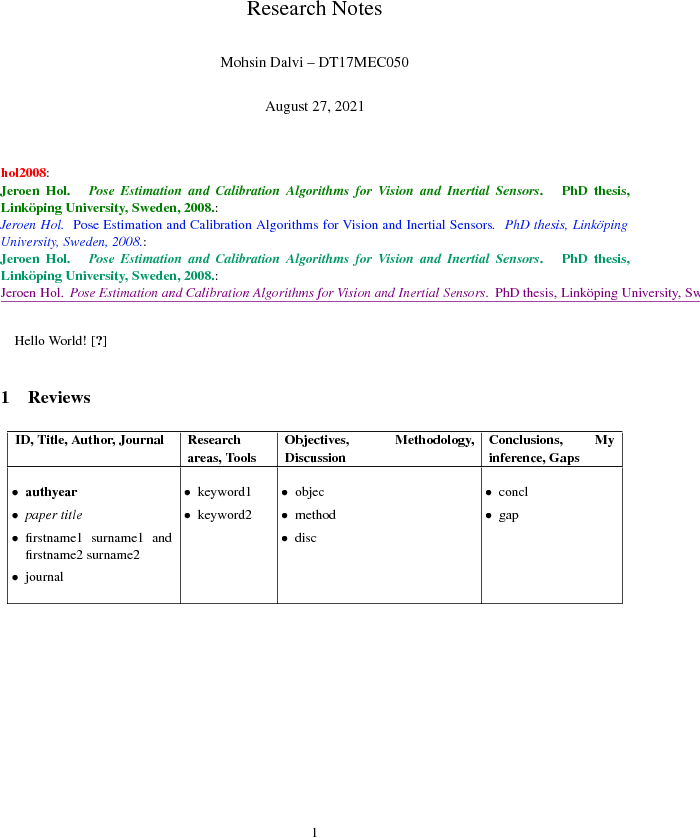
\includegraphics{image1}%
%
\hskip 10pt % insert a non-breaking space of specified width.
%
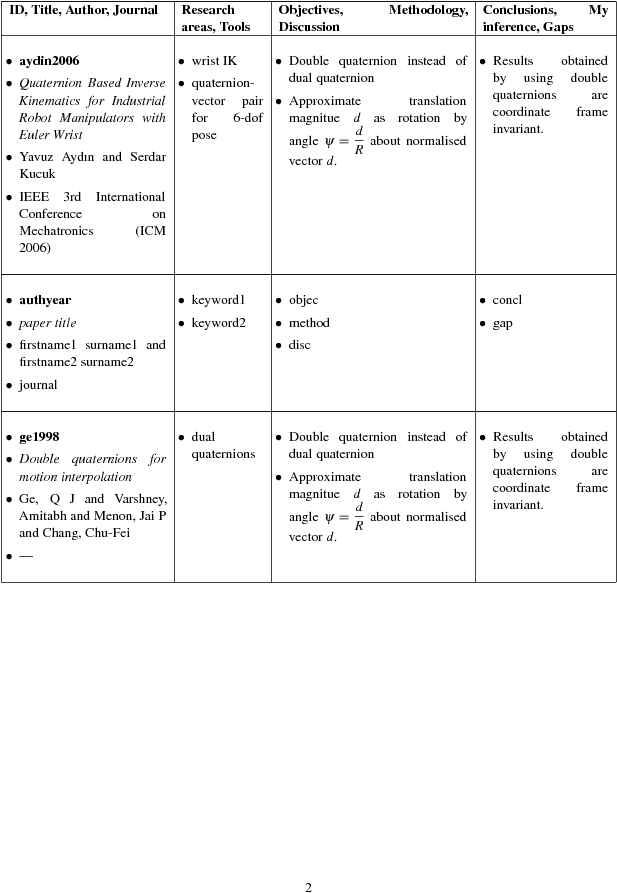
\includegraphics{image2}
\end{codeexample}
%
to place two graphics next to each other. This here is just the same (except
that our graphics occupy more code in the |.tex| file).

Note that there is also a comment sign after |\end{tikzpicture}|. This is not
just a best practice: it is necessary to suppress spurious spaces! In \TeX{},
every newline character is automatically converted to a white space (unless you
have an empty line, of course). In our case, we want no white spaces.

In our second picture, we see the effects of switch our math expression to
constant definitions as promised earlier. The interesting part starts with two
constants which are defined by means of two |\newcommand|s: we define |\MU| to
be 0 and |\SIGMA| to be |1e-3|. This is one way to define constants (note that
such a definition of constants should probably introduce round braces if
numbers are negative, i.e.\@ something like |\newcommand\negative{(-4)}|).


\subsection{Fixing the Vertical Alignment and Adjusting Tick Label Positions}
\label{sec:tut1:step4}

Note that even though our individual pictures look quite good, the combination
of both is not properly aligned. The experienced reader identifies the weak
point immediately: the bounding box of the two images differs, and they are
aligned at their baseline (which is the bottom edge of the picture). In
particular, the |xlabel=$x$| of the left picture and the automatically inserted
scaling label |\cdot 10^{-3}| of the right picture cause an unwanted vertical
shift. We want to fix that in the next step.

Besides the bad alignment, we find it a little bit misleading that the axis
descriptions of the second picture are between both pictures. We would like to
move them to the right.

Let us present the result first:
%
\begin{codeexample}[]
\begin{tikzpicture}[baseline]
    \begin{axis}[
        title=Inv. cum. normal,
        xlabel={$x$},
        ylabel={$y$},
        ymin=-3, ymax=3,
        minor y tick num=1,
    ]
        \addplot [blue] table {invcum.dat};
    \end{axis}
\end{tikzpicture}%
%
\hskip 10pt % insert a non-breaking space of specified width.
%
\begin{tikzpicture}[baseline]
    \begin{axis}[
        yticklabel pos=upper,
    ]
        % density of Normal distribution:
            \newcommand\MU{0}
            \newcommand\SIGMA{1e-3}
        \addplot [red,domain=-3*\SIGMA:3*\SIGMA,samples=201]
            {exp(-(x-\MU)^2 / 2 / \SIGMA^2) / (\SIGMA * sqrt(2*pi))};
    \end{axis}
\end{tikzpicture}
\end{codeexample}
%
This listing has a couple of modifications. The most important one is the we
added an option list to the |tikzpicture| environment: the |baseline| option.
This option shifts the picture up or down such that the canvas coordinate $y=0$
is aligned at the baseline of the surrounding text. In \PGFPlots{}, the $y=0$
line is the lower edge of the box. This simple feature allows both axes to be
aligned vertically: now, their boxes are aligned rather than the lower edges of
their bounding boxes. The option baseline needs to be provided to all pictures
for which this shifting should be done -- in our case, to all which are to be
placed in one row. Keep in mind that it is an option for |\begin{tikzpicture}|.

The second change is rather simple: we only added the option
|yticklabel pos=upper| to the second axis. This moves all tick labels to the
right, without changing anything else.

Note that there is much more to say about alignment and bounding box control.
After all, we did not really change the bounding box -- we simply moved the
pictures up or down. There is also the use case where we want horizontal
alignment: for example if the two pictures should be centered horizontally or
if they should be aligned with the left- and right end of the margins. The
associated keys |\begin{tikzpicture}[trim axis left, trim axis right]| and
|\centering| are beyond the scope of this tutorial, please refer to
Section~\ref{pgfplots:sec:align} for details.


\subsection{Satisfying Different Tastes}
\label{sec:tut1:step5}

We are now in a position where the figures as such are in a good shape.

However, an increase in knowledge will naturally lead to an increase in
questions. Some of these questions will be part of other how-to lectures. But
the most commonly asked questions are addressed here (feel free to email some
more if you believe that I should include another hotspot):
%
\begin{enumerate}
    \item How can I get rid of that $10^{-3}$ label?
    \item How can I modify the number printing?
    \item How can I have one single line per axis rather than a box?
\end{enumerate}

This here gives brief hints where to look in this reference manual for more
details. We modify the appearance of the second picture according to the
questions above:
%
\begin{codeexample}[]
\begin{tikzpicture}
\begin{axis}[
    axis lines=left,
    scaled ticks=false,
    xticklabel style={
        rotate=90,
        anchor=east,
        /pgf/number format/precision=3,
        /pgf/number format/fixed,
        /pgf/number format/fixed zerofill,
    },
]
    % density of Normal distribution:
        \newcommand\MU{0}
        \newcommand\SIGMA{1e-3}
  \addplot [red,domain=-3*\SIGMA:3*\SIGMA,samples=201]
        {exp(-(x-\MU)^2 / 2 / \SIGMA^2)
            / (\SIGMA * sqrt(2*pi))};
\end{axis}
\end{tikzpicture}
\end{codeexample}

The appearance of the axes as such can be controlled by means of the
|axis lines| key. It accepts the values |left, right, box, center, none| (and
also |top, bottom, middle| which are aliases). The |xticklabel style| key
modifies a predefined style (note the use of indentation here!). A style is a
collection of keys which are applied in a specific context. Styles are very
useful and are widely used by \PGFPlots{}. In our case, we adjust a couple of
options like rotation, alignment (the |anchor| option), and number printing
options. The precise details of these individual options is beyond the scope of
this tutorial. The keys actually belong to \Tikz{} -- and the \Tikz{} manual is
the reference for these keys (although \PGFPlots{} also covers most of the
topics). The complete set of number printing options is available in both the
\Tikz{} manual~\cite{tikz} and the manual for \PGFPlotstable{} which is shipped
with \PGFPlots{}. A brief extract can be found in
Section~\ref{sec:number:printing}.


\subsection{Finishing Touches: Automatic Generation of Individual Pdf Graphics}
\label{sec:tut1:step6}

As last step in this lecture, I would like to talk about one technical topic.
Typically, a \TeX{} document starts quite simple: a little bit of text, perhaps
one or two pictures. But they tend to grow. And eventually, you will encounter
one of the weak points of \PGFPlots{}: the graphics are involved and \TeX{}
consumes a lot of time to generate them. Especially if it keeps regenerating
them even though they did not change at all. The fact that we need to rerun the
pdflatex processor all the time makes things worse.

Fortunately, there are solutions. A simple solution is: why can't we write each
individual graphics into a separate |.pdf| file and use |\includegraphics| to
include it!? The answer is: yes, we can. And it is surprisingly simple to do
so.

In order to convert every |tikzpicture| environment automatically to an
external graphics \emph{without} changing any line of code in the \TeX{} file,
we can simply write the following two lines into the document's preamble:
%
\begin{codeexample}[code only]
\usepgfplotslibrary{external}
\tikzexternalize

...
\begin{document}
...
\end{document}
\end{codeexample}
%
But now, we \emph{have to provide a command line switch to pdflatex}:
%
\begin{codeexample}[code only]
pdflatex -shell-escape myfile.tex
\end{codeexample}

This works out of the box with |pdflatex|. If you use |latex/dvips|,
|lualatex|, |dvipdfm| or any other \TeX{} derivatives, you need to modify the
option |\tikzexternalize[system call=...]| (which is, unfortunately,
system-dependent, especially for the postscript variants).

It might be too much to discuss how to define individual file names or how to
modify the file name generation strategy. There is also the
|\tikzexternalize[mode=list and make]| feature which generates a GNU Make file
to allow |\label/\ref| to things inside of the external graphics and which
supports the generation of all images in parallel (if you have a multi-core
PC).

Details of the |external| library can be found in
Section~\ref{sec:pgfplots:export} (but only a brief survey) and, in all depth,
in the \Tikz{} reference manual~\cite{tikz}.


\subsection{Summary}

We learned how to create a standard axis, and how to assign basic axis
descriptions. We also saw how to plot functions from a data table (in our case
a tab-separated file, but other delimiters as in CSV files are also supported)
and from math expressions. We saw that \PGFPlots{} does a reasonable good job
at creating a fully-featured axis automatically (like scaling the units
properly, choosing tick positions and labels). We also learned how to improve
vertical alignment and how to customize the appearance of an axis.

Next steps might be how to draw multiple plots into the same axis, how to
employ scatter plots of \PGFPlots{}, how to generate logarithmic axes, or how
to draw functions of two variables. Some of these aspects will be part of
further how-to lectures.


\section{Solving a Real Use Case: Scientific Data Analysis}

In this section, we assume that you did some scientific experiment. The
scientific experiment yielded three input data tables: one table for each
involved parameter $d=2$, $d=3$, $d=4$. The data tables contain ``degrees of
freedom'' and some accuracy measurement ``|l2_err|''. In addition, they might
contain some meta-data (in our case a column ``level''). For example, the data
table for $d=2$ might be stored in |data_d2.dat| and may contain
%
\begin{codeexample}[code only]
dof        l2_err     level
5          8.312e-02  2
17         2.547e-02  3
49         7.407e-03  4
129        2.102e-03  5
321        5.874e-04  6
769        1.623e-04  7
1793       4.442e-05  8
4097       1.207e-05  9
9217       3.261e-06  10
\end{codeexample}
%
The other two tables are similar, we provide them here to simplify the
reproduction of the examples. The table for $d=3$ is stored in |data_d3.dat|,
it is
%
\begin{codeexample}[code only]
dof        l2_err     level
7          8.472e-02  2
31         3.044e-02  3
111        1.022e-02  4
351        3.303e-03  5
1023       1.039e-03  6
2815       3.196e-04  7
7423       9.658e-05  8
18943      2.873e-05  9
47103      8.437e-06  10
\end{codeexample}
%
Finally, the last table is |data_d4.dat|
%
\begin{codeexample}[code only]
dof        l2_err     level
9          7.881e-02  2
49         3.243e-02  3
209        1.232e-02  4
769        4.454e-03  5
2561       1.551e-03  6
7937       5.236e-04  7
23297      1.723e-04  8
65537      5.545e-05  9
178177     1.751e-05  10
\end{codeexample}

What we want is to produce three plots, each dof versus |l2_err|, in a loglog
plot. We expect that the result is a line in a log--log plot, and we are
interested in its slope $\log e(N) = -a \log(N)$ because that characterizes our
experiment.


\subsection{Getting the Data into \TeX{}}
\label{sec:tut2:step1}

Our first step is to get one of our data tables into \PGFPlots{}. In addition,
we want axis descriptions for the $x$- and $y$-axes and a title on top of the
plot.

Our first version looks like
%
\begin{codeexample}[]
%\documentclass{article}
%\usepackage{pgfplots}
%\pgfplotsset{compat=1.5}

%\begin{document}

\begin{tikzpicture}
\begin{loglogaxis}[
    title=Convergence Plot,
    xlabel={Degrees of freedom},
    ylabel={$L_2$ Error},
]
    \addplot table {data_d2.dat};
\end{loglogaxis}
\end{tikzpicture}

%\end{document}
\end{codeexample}

Our example is similar to that of the lecture in Section~\ref{sec:tut1:step1}
in that it defines some basic axis descriptions by means of |title|, |xlabel|,
and |ylabel| and provides data using |\addplot table|. The only difference is
that we used |\begin{loglogaxis}| instead of |\begin{axis}| in order to
configure logarithmic scales on both axes. Note furthermore that we omitted any
options after |\addplot|. As explained in Section~\ref{sec:tut1:step1}, this
tells \PGFPlots{} to consult its |cycle list| to determine a suitable option
list.


\subsection{Adding the Remaining Data Files of Our Example.}
\label{sec:tut2:step2}

\PGFPlots{} accepts more than one |\addplot ... ;| command -- so we can just
add our remaining data files:
%
\begin{codeexample}[]
\begin{tikzpicture}
\begin{loglogaxis}[
    title=Convergence Plot,
    xlabel={Degrees of freedom},
    ylabel={$L_2$ Error},
]
    \addplot table {data_d2.dat};
    \addplot table {data_d3.dat};
    \addplot table {data_d4.dat};
\end{loglogaxis}
\end{tikzpicture}
\end{codeexample}

You might wonder how \PGFPlots{} chose the different line styles. And you might
wonder how to modify them. Well, if you simply write |\addplot| without options
in square brackets, \PGFPlots{} will automatically choose styles for that
specific plot. Here ``automatically'' means that it will consult its current
|cycle list|: a list of predefined styles such that every |\addplot| statement
receives one of these styles. This list is customizable to a high degree.

Instead of the |cycle list|, you can easily provide style options manually. If
you write

|\addplot[|\meta{options}|] ...|,

\PGFPlots{} will only use \meta{options} and will ignore its |cycle list|. If
you write a plus sign before the square brackets as in

|\addplot+[|\meta{options}|] ...|,

\PGFPlots{} will append \meta{options} to the automatically assigned cycle
list.


\subsection{Add a Legend and a Grid}
\label{sec:tut2:step3}

A legend is a text label explaining what the plots are. A legend can be
provided for one or more |\addplot| statements using the |legend entries| key:
%
\begin{codeexample}[]
\begin{tikzpicture}
\begin{loglogaxis}[
    title=Convergence Plot,
    xlabel={Degrees of freedom},
    ylabel={$L_2$ Error},
    grid=major,
    legend entries={$d=2$,$d=3$,$d=4$},
]
    \addplot table {data_d2.dat};
    \addplot table {data_d3.dat};
    \addplot table {data_d4.dat};
\end{loglogaxis}
\end{tikzpicture}
\end{codeexample}
%
Here, we assigned a comma-separated list of text labels, one for each of our
|\addplot| instructions. Note the use of math mode in the text labels. Note
that if any of your labels contains a comma, you have to surround the entry by
curly braces. For example, we could have used
|legend entries={{$d=2$},{$d=3$},{$d=4$}}| -- \PGFPlots{} uses these braces to
delimit arguments and strips them afterwards (this holds for any option, by the
way).

Our example also contains grid lines for which we used the |grid=major| key. It
activates major grid lines in all axes.

You might wonder how the text labels map to |\addplot| instructions. Well, they
are mapped by index. The first label is assigned to the first plot, the second
label to the second plot and so on. You can exclude plots from this counting if
you add the |forget plot| option to the plot (using |\addplot+[forget plot]|,
for example). Such plots are excluded from both cycle lists and legends.


\subsection{Add a Selected Fit-line}
\label{sec:tut2:step4}

Occasionally, one needs to compute linear regression lines through input
samples. Let us assume that we want to compute a fit line for the data in our
fourth data table (|data_d4.dat|). However, we assume that the interesting part
of the plot happens if the number of degrees of freedom reaches some asymptotic
limit (i.e.\@ is very large). Consequently, we want to assign a high
uncertainty to the first points when computing the fit line.

\PGFPlots{} offers to combine table input and mathematical expressions (note
that you can also type pure mathematic expressions, although this is beyond the
scope of this example). In our case, we employ this feature to create a
completely new column -- the linear regression line:

\begin{codeexample}[]
%\usepackage{pgfplotstable}
%...
\begin{tikzpicture}
\begin{loglogaxis}[
    title=Convergence Plot,
    xlabel={Degrees of freedom},
    ylabel={$L_2$ Error},
    grid=major,
    legend entries={$d=2$,$d=3$,$d=4$},
]
    \addplot table {data_d2.dat};
    \addplot table {data_d3.dat};
    \addplot table {data_d4.dat};
    \addplot table [
      x=dof,
      y={create col/linear regression={y=l2_err,
       variance list={1000,800,600,500,400,200,100}}}]
        {data_d4.dat};
\end{loglogaxis}
\end{tikzpicture}
\end{codeexample}

Note that we added a further package: |pgfplotstable|. It allows to postprocess
tables (among other things. It also has a powerful table typesetting toolbox
which rounds and formats numbers based on your input CSV file).

Here, we added a fourth plot to our axis. The first plot is also an
|\addplot table| statement as before -- and we see that it loads the data file
|data_d4.dat| just like the plot before. However, it has special keys which
control the coordinate input: |x=dof| means to load x coordinates from the
column named ``dof''. This is essentially the same as in all of our other plots
(because the ``dof'' column is the first column). It also uses
|y={create col/...}|. This lengthy statement defines a completely new column.
The |create col/linear regression| prefix is a key which can be used whenever
new table columns can be generated. As soon as the table is queried for the
first time, the statement is evaluated and then used for all subsequent rows.
The argument list for |create col/linear regression| contains the column name
for the function values |y=l2_err| which are to be used for the regression line
(the x arguments are deduced from |x=dof| as you guessed correctly). The
|variance list| option is optional. We use it to assign variances
(uncertainties) to the first input points. More precisely: the first
encountered data point receives a variance of 1000, the second 800, the third
600, and so on. The number of variances does not need to match up with the
number of points; \PGFPlots{} simply matches them with the first encountered
coordinates.

Note that since our |legend entries| key contains only three values, the
regression line has no legend entry. We could easily add one, if we wanted. We
can also use |\addplot+[forget plot] table[...]| to explicitly suppress the
generation of a legend as mentioned above.

Whenever \PGFPlots{} encounters mathematical expressions, it uses its built-in
floating point unit. Consequently, it has a very high data range -- and a
reasonable precision as well.


\subsection{Add an Annotation using \Tikz{}: a Slope Triangle}
\label{sec:tut2:step5}

Often, data requires interpretation -- and you may want to highlight particular
items in your plots. This ``highlight particular items'' requires to draw into
an axis, and it requires a high degree of flexibility. Users of \Tikz{} would
say that \Tikz{} is a natural choice -- and it is.

In our use case, we are interested in slopes. We may want to compare slopes of
different experiments. And we may want to show selected absolute values of
slopes.

Here, we use \Tikz{} to add custom annotations into a \PGFPlots{} axis. We
choose a particular type of a custom annotation: we want to mark two points on
a line plot. One way to do so would be to determine the exact coordinates and
to place a graphical element at this coordinate (which is possible using
|\draw ... (1e4,1e-5) ... ;|). Another (probably simpler) way is to use the
|pos| feature to identify a position ``25\% after the line started''.

Based on the result of Section~\ref{sec:tut2:step4}, we find
%
\begin{codeexample}[]
%\usepackage{pgfplotstable}
%...
\begin{tikzpicture}
\begin{loglogaxis}[
    title=Convergence Plot,
    xlabel={Degrees of freedom},
    ylabel={$L_2$ Error},
    grid=major,
    legend entries={$d=2$,$d=3$,$d=4$},
]
    \addplot table {data_d2.dat};
    \addplot table {data_d3.dat};
    \addplot table {data_d4.dat};
    \addplot table [
      x=dof,
      y={create col/linear regression={y=l2_err,
       variance list={1000,800,600,500,400,200,100}}}]
        {data_d4.dat}
            % save two points on the regression line
            % for drawing the slope triangle
            coordinate [pos=0.25] (A)
            coordinate [pos=0.4]  (B)
   ;
    % save the slope parameter:
    \xdef\slope{\pgfplotstableregressiona}

    % draw the opposite and adjacent sides
    % of the triangle
    \draw (A) -| (B)
         node [pos=0.75,anchor=west]
         {\pgfmathprintnumber{\slope}};
\end{loglogaxis}
\end{tikzpicture}
\end{codeexample}

The example is already quite involved since we added complexity in every step.
Before we dive into the details, let us take a look at a simpler example:
%
\begin{codeexample}[]
\begin{tikzpicture}
\begin{loglogaxis}
    \addplot table {data_d2.dat}
       coordinate [pos=0.25] (A)
       coordinate [pos=0.4]  (B)
    ;

    \draw [-stealth] (A) -| (B);

    \node [pin=0:Special.] at (769,1.623e-04) {};
\end{loglogaxis}
\end{tikzpicture}
\end{codeexample}
%
Here, we see two annotation concepts offered by \PGFPlots{}: the first is to
insert drawing commands right after an |\addplot| command (but before the
closing semicolon). The second is to add standard \Tikz{} commands, but use
designated \PGFPlots{} coordinates. Both are \Tikz{} concepts. The first is
what we want here: we want to identify two coordinates which are ``somewhere''
on the line. In our case, we define two named coordinates: coordinate $A$ at
25\% of the line and coordinate $B$ at 40\% of the line. Then, we use
\verb#\draw (A) -| (B)# to draw a triangle between these two points. The second
is only useful if we know some absolute coordinates in advance.

Coming back to our initial approach with the regression line, we see that it
uses the first concept: it introduces named coordinates after |\addplot|, but
before the closing semicolon. The statement |\xdef\slope| introduces a new
macro. It contains the (expanded due to the ``eXpanded DEFinition'') value of
|\pgfplotstableregressiona| which is the slope of the regression line. In
addition to the slope triangle, we also add a node in which we typeset that
value using |\pgfmathprintnumber|.

Note that the example above is actual a ``happy case'': it can happen easily
that labels which are added inside of the axis environment are clipped away:
%
\begin{codeexample}[]
\begin{tikzpicture}
\begin{loglogaxis}[
    tiny,
]
    \addplot table {data_d2.dat}
        node [pos=1,pin=0:Special.] {}
    ;
\end{loglogaxis}
\end{tikzpicture}
\end{codeexample}
%
The example above combines the |pos| label placement with the node's label.
Note that the small style |tiny| installs a \PGFPlots{} preset which is better
suited for very small plots -- it is one of the many supported scaling
parameters. The problem here is apparent: the text of our extra node is clipped
away. Depending on your data, you have a couple of solutions here:
%
\begin{itemize}
    \item use |clip=false| to disable clipping of plot paths at all,
    \item use |clip mode=individual| to enable clipping only for plot paths,
    \item draw the node outside of the axis environment but inside of the
        picture environment.
\end{itemize}
%
The first attempt works quite well for most figures:
%
\begin{codeexample}[]
\begin{tikzpicture}
\begin{loglogaxis}[
    tiny,
    clip=false,
]
    \addplot table {data_d2.dat}
        node [pos=1,pin=0:Special.] {}
    ;
\end{loglogaxis}
\end{tikzpicture}
\end{codeexample}
%
Note that this approach in which the nodes are placed before the closing
semicolon implies that nodes inherit the axis line style and color.


\subsection{Summary}

We learned how to define a (logarithmic) axis, and how to assign basic axis
descriptions. We also saw once more how to use one or more |\addplot table|
commands to load table data into \PGFPlots{}. We took a brief look into
regression and \Tikz{} drawing annotations.

We also encountered the |tiny| style which is one of the ways to customize the
size of an axis. Others are |width|, |height|, the other predefined size styles
like |normalsize|, |small|, or |footnotesize|, and the two different scaling
modes |/pgfplots/scale| and |/tikz/scale| (the first scales only the axis, the
second also the labels).

Next steps might be how to visualize functions using line plots, how to align
adjacent graphics properly (even if the axis descriptions vary), how to employ
scatter plots of \PGFPlots{}, or how to draw functions of two variables.

%The steps are explained in all detail in the reference
%Chapter~\ref{cha:pgfplots:reference}.


\section{Use Cases involving Scatter Plots}

Assuming that we are more or less familiar with the basics of the preceding
tutorials, we would like to draw a scatter plot. A scatter plot is one in which
markers indicate the important information.

There are many different kinds of scatter plots and this section covers a
couple of them.

\subsection{Scatter Plot Use Case A}
\label{sec:tut3:usecaseA}

In this subsection, we address the following scatter plot use case: assume that
we are given a couple of special $(x,y)$ coordinates along with color data at
every vertex. We would like to draw markers at the positions and choose
individual colors depending on the color data.


\subsubsection{Importing the Data File}

We assume that our input data is given as a table containing much more columns
than we need. The first couple of rows are as follows:

    \lstinputlisting[
        columns=fixed,
        breaklines=false,
        tabsize=15,
        lastline=8,
            ]{plotdata/concat_VV_together_grid.dat}

What we need is the first and second column to get the $x$- and $y$-coordinate
values, respectively, and the third column |f(x)| to choose color values. The
color values are very small and have a high range: there are values of order
$10^{-6}$ and there are values of order $1$. Such ranges are best shown on a
logarithmic scale, which is why we will resort to some logarithmic scale on the
absolute values of this column. Thus, a requirement will be to accept a math
expression (involving logs) on the color data column.

Note that the data file (and all others referenced in this manual) are shipped
with \PGFPlots{}; you can find them in the subfolder
\texttt{doc/latex/pgfplots/plotdata}.

We learned already how to read table data from a file, so our first step is
relatively straightforward.

\begin{codeexample}[]
\begin{tikzpicture}
\begin{axis}
    \addplot+ [only marks] table
        {concat_VV_together_grid.dat};
\end{axis}
\end{tikzpicture}
\end{codeexample}

Here, the only non-trivial variation is the option |only marks| which is given
after the plus sign. Keep in mind that |\addplot+[|\meta{options}|]| means that
\PGFPlots{} shall combine the set of options of its |cycle list| with
\meta{options}. In our case, |only marks| does what it says. The |only marks|
plot handler is the most simple scatter plot: it uses the same color for every
marker.

Note that |\addplot table| takes the first column as |x| and the second as |y|
(which matches our input file perfectly).


\subsubsection{Fine Tuning}

We agree that our initial import has unsuitable displayed limits: there is too
much white space around the interesting plot area. In addition, the markers
overlap because they are too large. We can modify the appearance as follows:

\begin{codeexample}[]
\begin{tikzpicture}
\begin{axis}[
    enlargelimits=false,
]
    \addplot+ [only marks,mark size=0.6pt]
        table {concat_VV_together_grid.dat};
\end{axis}
\end{tikzpicture}
\end{codeexample}

As before, we assume that we add more options after |\begin{axis}|.
Consequently, we introduced suitable indentation and a trailing comma after the
option. Note that |enlargelimits| is typically active; it means that
\PGFPlots{} increases the displayed range by $10\%$ by default. Deactivating it
produces tight limits according to the input data.

Our second option is |mark size| -- using an absolute size (about the radius or
half size of the marker).


\subsubsection{Color Coding According To Input Data}

We are quite close to our goal, except for the colors. As discussed, our input
file contains three columns and the third one should be used to provide color
information. In our case, the data file has a column named |f(x)|.
%
\begin{codeexample}[]
\begin{tikzpicture}
    \begin{axis}[
        enlargelimits=false,
        colorbar,
    ]
        \addplot+ [
            only marks,
            scatter,
            point meta={
                ln(1e-6+abs(\thisrow{f(x)}))/ln(10)
            },
            mark size=0.6pt,
        ] table {concat_VV_together_grid.dat};
    \end{axis}
\end{tikzpicture}
\end{codeexample}
%
We added a couple of options to our example: the options |scatter|, and
|point meta|, |colorbar|. The option |scatter| has a slightly misleading name as
we already had a scatter plot before we added that option. It activates scatter
plots with individual appearance: without further options, it chooses
individual colors for every marker. The ``individual colors'' are based on
something which is called ``|point meta|'' in \PGFPlots{}. The |point meta| is
typically a scalar value for every input coordinate. In the default
configuration, it is interpreted as ``color data'' for the coordinate in
question. This also explains the other option: |point meta=...| tells
\PGFPlots{} which values are to be used to determine colors. Note that the
default value of |point meta| is to use the $y$~coordinate. In our case, we
have a complicated math expression which is related to our input file: it
contains small quantities in column |f(x)| which are based shown on a
logarithmic scale as their differ over a huge range. Since a logarithm must not
have a non-positive argument, we have $10^{-6} + \text{abs}(\dotsb)$ as
expression which ensures that the argument is never smaller than |10^{-6}| and
that is is positive. The divider |/ln(10)| means that we have logarithms
base~$10$. But the key point of the whole complicated expression can be
summarized as follows:
%
\begin{enumerate}
    \item We can use |\thisrow|\marg{column name} to refer to table columns.
        Here, ``this row'' means to evaluate the table for the ``data point
        which is being read from the current row''.
    \item We can combine |\thisrow| with any complicated math expression.
\end{enumerate}
%
The third new option |colorbar| activates the color bar on the right hand side
(as you guessed correctly). We see that the smallest value is $-6$ which
corresponds to our value |1e-6| in the math expression.

You might wonder how a scalar value (the number stored in the |f(x)| column)
results in a color. \PGFPlots{} computes the minimum and maximum value of all
such numbers. Then, it maps every number into a |colormap|. A |colormap|
defines a couple of colors and interpolates linearly between such colors. That
means that the smallest value of |point meta| is mapped to the first color in a
|colormap| whereas the largest value of |point meta| is mapped to the last
color in the |colormap|. All others are mapped to something in-between.

More information about |colormap| and |point meta| can be found in
Section~\ref{sec:colormap:input:format} and in
Section~\ref{pgfplots:point:meta}.


\subsection{Scatter Plot Use Case B}

As already mentioned, there are various use cases for scatter plots. The
default configuration of the |scatter| key is to read numeric values of
|point meta| and choose colors by mapping that value into the current |colormap|.

A different application would be to expect symbolic input (some string) and
choose different markers depending on that input symbol.

Suppose that you are given a sequence of input coordinates of the form $(x,y)$
\meta{class label} and that you want to choose marker options depending on the
\meta{class label}. A \PGFPlots{} solution could be
%
\begin{codeexample}[]
\begin{tikzpicture}
\begin{axis}
    \addplot [
        scatter,
        only marks,
        point meta=explicit symbolic,
        scatter/classes={
            a={mark=square*,blue},
            b={mark=triangle*,red},
            c={mark=o,draw=black}% <-- don't add comma
        },
    ] table [meta=label] {
        x      y        label
        0.1    0.15     a
        0.45   0.27     c
        0.02   0.17     a
        0.06   0.1      a
        0.9    0.5      b
        0.5    0.3      c
        0.85   0.52     b
        0.12   0.05     a
        0.73   0.45     b
        0.53   0.25     c
        0.76   0.5      b
        0.55   0.32     c
    };
\end{axis}
\end{tikzpicture}
\end{codeexample}
%
As in our previous use case in Section~\ref{sec:tut3:usecaseA}, we have the
options |scatter|, |only marks|, and a configuration how to retrieve the
|point meta| values by means of the |meta| key. One new key is
|point meta=explicit symbolic|: it tells \PGFPlots{} that any encountered values
of |point meta| are to be interpreted as string symbols. Furthermore, it tells
\PGFPlots{} that the every input coordinate comes with an explicit value (as
opposed to a common math expression, for example). The other different option
is |scatter/classes|. As you guessed from the listing, it is a map from string
symbol to marker option list. This allows to address such use cases in a simple
way.

This example has actually been replicated from the reference manual section for
|scatter/classes|.


\subsection{Scatter Plot Use Case C}

Finally, this tutorial sketches a further use case for scatter plots: given a
sequence of coordinates $(x,y)$ with individual string labels, we want to draw
the string label at the designated positions.

This can be implemented by means of the |nodes near coords| feature of
\PGFPlots{}, which is actually based on |scatter|:
%
\begin{codeexample}[]
\begin{tikzpicture}
\begin{axis}[
    enlargelimits=0.2,
]
    \addplot+ [nodes near coords,only marks,
       point meta=explicit symbolic]
    table [meta=label] {
        x    y   label
        0.5  0.2 1
        0.2  0.1 t2
        0.7  0.6 3
        0.35 0.4 Y4
        0.65 0.1 5
    };
\end{axis}
\end{tikzpicture}
\end{codeexample}
%
In this case, we have |point meta=explicit symbolic| in order to express the
fact that our labels are of textual form (see the reference manual section for
|nodes near coords| for applications of \emph{numeric} labels). The remaining
stuff is done by the implementation of |nodes near coords|. Note that enlarged
the axis limits somewhat in order to include the text nodes in the visible
area.

There is much more to say about |scatter| plots, and about |nodes near coords|.
Please consider this subsection as a brief pointer to
Section~\ref{sec:pgfplots:scatter:2d} in the reference manual.


\subsection{Summary}

We learned how to generate scatter plots with single color using |only marks|,
scatter plots with individually colored markers using the |scatter| key,
scatter plots with specific marker styles depending on some class label using
|scatter/classes| and text nodes using |nodes near coords|.

Furthermore, we introduced the concept of ``|point meta| data'': once as
(scalar valued) color data, once as symbolic class label and once as text
label.

There is much more to say, especially about |point meta| which is introduced
and explained in all depth in Section~\ref{pgfplots:point:meta}.

There is also more to say about |scatter| plots, for example how to generate
scatter plots with individually sized markers and/or colors (by relying on
|\pgfplotspointmetatransformed|, see the reference manual section for
|visualization depends on|). In addition, |scatter| plots can be customized to
a high degree which is explained in Section~\ref{sec:pgfplots:scatter:2d}.


\section{Solving a Real Use Case: Functions of Two Variables}

In this tutorial, we assume that we have two functions for which we seek a
plot: the first is a sampled function given by a huge data file and the second
is the math expression $g(x,y)=\exp(-x^2-y^2)\cdot x$.

Our first function actually consists of two data files: the first file contains
some scattered data which resembles a discretization (``sampling'') of a
function and the second file contains data for the function as such, sampled on
a lattice. Our requirement here is two draw \emph{two} graphs into the same
axis: one in which the function is plotted as a smooth, colored surface and one
in which the scattered data file should be on top of the surface because it
provides more detail how the function was represented in the computer.

The second function which is given as math expression should be visualized
using a contour plot. A contour plot expects some fixed values $g_1, \dotsc,
g_k$ as input (the contour values) and plots one curve for each $g_j = g(x,y)$
(i.e.\@ if you go hiking without ever changing the height of your path).


\subsection{Surface Plot from Data File}

Our first step is to load the data file and to plot a surface.

Clearly, functions of two variables require a more sophisticated input format:
they are typically sampled on a unified grid with $n \times m$ points, i.e.\@
$n$~points for $x$ and $m$~points for $y$, resulting in a total of matrix with
$n\cdot m$ values $f_{ij} = f(x_i,y_i)$. How can we read matrix data? And what
if you have more than just the $z$ value? A standard way is to write the matrix
to a table, either in line by line ordering or in column by column ordering
(both are common).

Here, we assume that our function values are written to a table in which the
$y$ values vary from line to line. Here is an extract of the data file (which
is too large to list it here):

    \lstinputlisting[
        columns=fixed,
        breaklines=false,
        firstline=1,
        tabsize=15,
        lastline=6,
    ]{plotdata/concat_VV_together.dat}%
        \vskip-0.9\baselineskip
            $\vdots$
        \vskip-0.4\baselineskip
    \lstinputlisting[
        columns=fixed,
        breaklines=false,
        firstline=34,
        tabsize=15,
        lastline=43,
    ]{plotdata/concat_VV_together.dat}%
        \vskip-0.9\baselineskip
            $\vdots$

Note that the data file (and all others referenced in this manual) are shipped
with \PGFPlots{}; you can find them in the subfolder
\texttt{doc/latex/pgfplots/plotdata}.

The input file contains $x_0$, $x_1$, and $f(x_0,x_1)$ in columns named |x_0|,
|x_1|, and |f(x)|, respectively. In addition, it contains some meta data which
is irrelevant for us here.

Note that our input file contains \emph{empty lines} whenever |x_0| changes.
This is a common data format which simplifies the detection of ``scanline
length''. A scanline is one line in the input matrix, for example the line
consisting of all points with $x_0 = 0$. With such scanlines, \PGFPlots{} can
automatically deduce the size of the input matrix.

In order to plot the file as a surface, we proceed as in the previous example
by using |\addplot table|. However, we have to use |\addplot3| to indicate that
a three-dimensional result is expected: \pgfplotsexpensiveexample
%
\begin{codeexample}[]
\begin{tikzpicture}
\begin{axis}
    \addplot3 [
        surf,
        mesh/ordering=y varies,
    ] table {concat_VV_together.dat};
\end{axis}
\end{tikzpicture}
\end{codeexample}
%
The example looks familiar compared to our results of the preceding tutorials:
a |tikzpicture| environment containing an |axis| environment and the mentioned
|\addplot3| command. The option list contains |surf|, which tells \PGFPlots{}
how to visualize the input data. The key |mesh/ordering=y varies| tells
\PGFPlots{} how to decode the input matrix. This is important; otherwise
\PGFPlots{} would have chosen |x varies| which does not match our file.

Note that we there is no need to configure either |mesh/rows=|\meta{N} or
|mesh/cols=|\meta{N} here because these parameters are automatically deduced
from the scan line lengths marked by empty lines in our input file.

Since our |\addplot3 table| statement does not contain any hints which columns
should be plotted, \PGFPlots{} simply plots the first three columns against
each other.

The colors of a |surf| plot are chosen from the function values (unless you
configure some other value for |point meta|; this is similar to the scatter
plot example). In case of a function of two variables, the function value is
the third column.


\subsection{Fine-Tuning}

In order to stress how colors are to be mapped to values, we add a color bar to
our example from the previous subsection. In addition, we rotate the view a
little bit and add axis labels. Furthermore, we would like to have a smooth
color mapping.

We end up at
%
\pgfplotsexpensiveexample
\begin{codeexample}[]
\begin{tikzpicture}
\begin{axis}[
    view/h=40,
    colorbar horizontal,
    xlabel=$x$, ylabel=$y$,
]
    \addplot3 [
        surf,
        mesh/ordering=y varies,
        shader=interp,
    ] table {concat_VV_together.dat};
\end{axis}
\end{tikzpicture}
\end{codeexample}
%
Here, |view/h| rotates the ``horizontal'' parts of the view (only). It chooses
a new view angle for the orthographic projection. As you guessed, there is also
a |view/v| key and a |view=|\marg{h}\marg{v} variant.

The key |colorbar horizontal| is a style which activates a |colorbar| and
configures it to be displayed horizontally. The labels are placed using
|xlabel| and |ylabel| as we saw it before for visualizations of one-dimensional
functions. A colorbar uses the current |colormap| and adds axis descriptions to
show how values are mapped to colors.

 The |shader=interp| key activates a smooth color interpolation.


\subsection{Adding Scattered Data on Top of the Surface}

As motivated earlier, we have a second data set, one which characterizes how
the function has been represented in some computer simulation. We would like to
add the second data set as scatter plot on top of the function.

The data set as such is the very same as the one used in
Section~\ref{sec:tut3:usecaseA}, so we do not need to list it here again.
However, we have to include the two-dimensional scatter data into the
three-dimensional axis in a suitable way. We chose to place it on a fixed $z$
value as follows:
%
\pgfplotsexpensiveexample
\begin{codeexample}[]
\begin{tikzpicture}
\begin{axis}[
    view/h=40,
    colorbar horizontal,
    xlabel=$x$, ylabel=$y$,
]
    \addplot3 [surf,mesh/ordering=y varies,
        shader=interp
    ] table {concat_VV_together.dat};

    \addplot3 [blue,mark=*,
        mark options={fill=blue!80!black},
        only marks,mark size=0.6pt,
    ] table [z expr=1.2]{concat_VV_together_grid.dat};
\end{axis}
\end{tikzpicture}
\end{codeexample}
%
Now, we have two |\addplot3 table| statements in the same axis. None of them
uses the |cycle list| as we used explicit option lists. The first is our
surface plot. Note that it is plotted before the scatter plot: \PGFPlots{}
cannot handle depth information between adjacent |\addplot| statements. It
does, however, handle |z buffer| information for data of a single |\addplot|
statement. The second plot is our scatter plot: we recognize |only marks| and
|mark size| from Section~\ref{sec:tut3:usecaseA}. In addition, we configured
some color and marker options.

An important aspect is |\addplot3 table[z expr=1.2]| -- it tells \PGFPlots{}
how to choose $z$ values for the input file (otherwise, \PGFPlots{} would have
used the third column of that file). This is a convenient way to insert
two-dimensional data into a three-dimensional axis, provided you have
\emph{table} data. There is also a different way which works for both tables
and math expressions (or other input types). This different way is to install a
|z filter|, but that is beyond the scope of this tutorial for now.


\subsection{Computing a Contour Plot of a Math Expression}

This section addresses the second part of our use case example: a function of
two variables given by a math expression.

Our function of interest is $x \exp(-x^2-y^2)$. We start as in our tutorial for
one-dimensional functions given by a math expression (compare
Section~\ref{sec:tut1:step3}): by using an |\addplot| statement which is
followed by a math expression in curly braces. However, we rely on |\addplot3|
as in the preceding section:

\pgfplotsexpensiveexample
\begin{codeexample}[]
\begin{tikzpicture}
\begin{axis}[
    title={$x \exp(-x^2-y^2)$},
    xlabel=$x$, ylabel=$y$,
    small,
]
    \addplot3 {exp(-x^2-y^2)*x};
\end{axis}
\end{tikzpicture}
\end{codeexample}
%
Our example contains a basic axis environment with |title|, |xlabel|, |ylabel|
and the |small| key which are already known from the preceding tutorials. The
|\addplot3| has no options and is immediately followed by the math expression.
The absence of options tells \PGFPlots{} to rely on its |cycle list|. This, in
turn configures |mark=*| with |blue| color -- and a line plot. A line plot
combined with |\addplot3| is of limited use; it merely connects all incoming
points. Since points are sampled as a matrix (line by line). Our next step will
be to define a suitable plot handler.

Note, however, that our math expression depends on |x| and |y|. These two
variables are the sampling variables of \PGFPlots{} in its default configures:
both are sampled in the |domain| of interest using the correct number of
|samples|. The |\addplot3| statement takes care of computing $N\cdot M$ points
in the correct sequence where $N$ is the number of |samples| for $x$ and $M$ is
|samples y|, the number of samples used for $y$.

We can see that our sampling |domain| is too large. Switching to a smaller
|domain| focusses on the interesting parts of our function:

\pgfplotsexpensiveexample
\begin{codeexample}[]
\begin{tikzpicture}
\begin{axis}[
    title={$x \exp(-x^2-y^2)$},
    xlabel=$x$, ylabel=$y$,
    small,
]
    \addplot3 [
        surf,
        domain=-2:2,
        domain y=-1.3:1.3,
    ] {exp(-x^2-y^2)*x};
\end{axis}
\end{tikzpicture}
\end{codeexample}
%
Here, we introduced an option list after |\addplot3|. Since we provided the
option list without the leading plus sign `|+|', \PGFPlots{} does not consider
its |cycle list| at all (and switches off |mark|s and the default color
settings). We added |domain| and |domain y| in order to restrict the sampling
domain in a suitable way. If we would have omitted |domain y|, the $y$ domain
would use the same value as the $x$ |domain|.

As you might have guessed, the |surf| key has the main use case of providing a
connection to the previous tutorial section: it is one of the natural
visualizations for functions of two variables. As in the preceding section, the
color has been deduced from the function value $z=f(x,y)$ (more precisely, by
relying on the default configuration |point meta=f(x)|).

The next step is to switch to contour plots by replacing `|surf|` by
`|contour lua|':

\pgfplotsexpensiveexample
\begin{codeexample}[]
\begin{tikzpicture}
\begin{axis}[
    title={$x \exp(-x^2-y^2)$},
    xlabel=$x$, ylabel=$y$,
    small,
]
    \addplot3 [
        contour lua,
        domain=-2:2,
        domain y=-1.3:1.3,
    ] {exp(-x^2-y^2)*x};
\end{axis}
\end{tikzpicture}
\end{codeexample}
%
Now, we have a contour plot -- although it is not quite what we had in mind.
First, there are so few contour lines that it is hard to see anything
(especially since the |line width| is too small). Furthermore, the |view|
direction is unfamiliar.

We add the |view| option with the argument for ``view from top'' and configure
the number of contour lines using the |contour/number| key and the |line width|
using the |thick| style:

\pgfplotsexpensiveexample
\begin{codeexample}[]
\begin{tikzpicture}
\begin{axis}[
    title={$x \exp(-x^2-y^2)$},
    enlarge x limits,
    view={0}{90},
    xlabel=$x$, ylabel=$y$,
    small,
	colorbar,
]
    \addplot3[
        domain=-2:2,
        domain y=-1.3:1.3,
        contour lua={number=14,labels=false},
        thick,
    ] {exp(-x^2-y^2)*x};
\end{axis}
\end{tikzpicture}
\end{codeexample}

This is what we wanted to achieve. Note that |contour lua| accepts options
which have the key prefix |contour/|. In this context, the prefix is optional.

Note that |contour lua| is different from almost all other plot handlers of
\PGFPlots{} with respect to one aspect: it requires you to invoke

|lualatex |\meta{texfilename}

\noindent instead of

|pdflatex |\meta{texfilename} .

\noindent 
The nonlinear algorithm to
compute contour lines is currently unavailable in plain \TeX{} which is stressed
by the name `|contour lua|'. 


If you cannot use |lualatex| for some reason, you can replace |contour lua| by |contour gnuplot|, provided that you have the external program |gnuplot| installed on your system (see the reference for |contour gnuplot| for more details).

\subsection{Summary}

We have sketched how to load a data table containing a sampled function of two
variables, and we learned how to visualize such data as |surf|ace plot. We
learned how to rotate the |view|, how to change the color |shader| of |surf|ace
plots, how to enabled |colorbar|s, and how to add |scatter| plots on top of
surface plots. Furthermore, we encountered the first contour plot as an example
for how to sample a function of two variables by means of built-in methods of
\PGFPlots{}.

It should be stressed that \PGFPlots{} needs no external tool to generate such
plots: every computer with a decent version of \PGFPlots{} can regenerate these plots.

There is more to say about three-dimensional axes, in particular regarding
|mesh/ordering|, parametric plots, perhaps line plots in three dimensions or
other plot types. Furthermore, there are some limitations regarding the
|z buffer|ing, i.e.\@ how \PGFPlots{} decides which parts of the figure are in
front of others. These items can be read in Section~\ref{sec:3d} and its
subsections.

You might also be interested in styles to change the appearance of a
three-dimensional axis, compare Section~\ref{sec:3d:axis:config}.

}%

% main=manual.tex

\chapter{The Reference}
\label{cha:pgfplots:reference}

{
\tikzset{external/figure name/.add={}{reference_}}


\section{\TeX{} dialects: \LaTeX{}, Con\TeX{}t, plain \TeX{}}
\label{sec:tex:dialects}

The starting point for \PGFPlots{} is an |axis| environment like |axis| or the
logarithmic variants |semilogxaxis|, |semilogyaxis| or |loglogaxis|.

Each environment is available for \LaTeX{}, Con\TeX{}t and plain \TeX{}:
%
\begin{description}
        \def\HEAD{%
            \small
            %\lstset{boxpos=b,breaklines=false,aboveskip=3pt,belowskip=3pt}%
            %\hspace{-1cm}%
            \begin{tabular}{*{2}{p{4cm}}}%
        }%
    \item[\LaTeX{}:]
        |\usepackage{pgfplots} \pgfplotsset{compat=|\pgfkeysvalueof{/pgfplots/compat/mostrecent}|}|
        and

        {\HEAD
\begin{codeexample}[code only]
\begin{tikzpicture}
\begin{axis}
...
\end{axis}
\end{tikzpicture}
\end{codeexample}
        &
\begin{codeexample}[code only]
\begin{tikzpicture}
\begin{semilogxaxis}
...
\end{semilogxaxis}
\end{tikzpicture}
\end{codeexample}
        \\
        \end{tabular}%
        }

        Here, the
        |\pgfplotsset{compat=|\pgfkeysvalueof{/pgfplots/compat/mostrecent}|}|
        key should be set to at least version 1.3. Otherwise \PGFPlots{}
        assumes that your document has been generated years ago and attempts
        to run in backwards compatibility mode as good as it can.

        Since \LaTeX{} is the default for many people, this manual only shows
        \LaTeX{} examples. A full document skeleton can be found below this
        enumeration.
    \item[Con\TeX{}t:]
        |\usemodule[pgfplots] \pgfplotsset[compat=|\pgfkeysvalueof{/pgfplots/compat/mostrecent}|]|
        and

        {\HEAD
\begin{codeexample}[code only]
\starttikzpicture
\startaxis
...
\stopaxis
\stoptikzpicture
\end{codeexample}
        &
\begin{codeexample}[code only]
\starttikzpicture
\startsemilogxaxis
...
\stopsemilogxaxis
\stoptikzpicture
\end{codeexample}
        \\
        \end{tabular}%
        }

        A complete Con\TeX{}t example file can be found in
        %
\begin{codeexample}[code only]
doc/context/pgfplots/pgfplotsexample.tex.
\end{codeexample}
        %
    \item[plain \TeX{}:]
        |\input pgfplots.tex \pgfplotsset{compat=|\pgfkeysvalueof{/pgfplots/compat/mostrecent}|}|
        and

        {\HEAD
\begin{codeexample}[code only]
\tikzpicture
\axis
...
\endaxis
\endtikzpicture
\end{codeexample}
        &
\begin{codeexample}[code only]
\tikzpicture
\semilogxaxis
...
\endsemilogxaxis
\endtikzpicture
\end{codeexample}
        \\
        \end{tabular}%
        }

        A complete plain \TeX{} example file can be found in
        %
\begin{codeexample}[code only]
doc/plain/pgfplots/pgfplotsexample.tex.
\end{codeexample}
\end{description}

For \LaTeX{}, a complete example will look somehow like this:
%
\begin{codeexample}[code only]
\documentclass[a4paper]{article}

% for dvipdfm:
%\def\pgfsysdriver{pgfsys-dvipdfm.def}
\usepackage{pgfplots}
\pgfplotsset{compat=1.6}% <-- moves axis labels near ticklabels (respects tick label widths)

\begin{document}
\begin{figure}
    \centering
    \begin{tikzpicture}
        \begin{loglogaxis}[xlabel=Cost,ylabel=Error]
            \addplot coordinates {
                (5,     8.31160034e-02)
                (17,    2.54685628e-02)
                (49,    7.40715288e-03)
                (129,   2.10192154e-03)
                (321,   5.87352989e-04)
                (769,   1.62269942e-04)
                (1793,  4.44248889e-05)
                (4097,  1.20714122e-05)
                (9217,  3.26101452e-06)
            };
            \addplot coordinates {
                (7,     8.47178381e-02)
                (31,    3.04409349e-02)
                (111,   1.02214539e-02)
                (351,   3.30346265e-03)
                (1023,  1.03886535e-03)
                (2815,  3.19646457e-04)
                (7423,  9.65789766e-05)
                (18943, 2.87339125e-05)
                (47103, 8.43749881e-06)
            };
            \legend{Case 1,Case 2}
        \end{loglogaxis}
    \end{tikzpicture}
    \caption{A larger example}
\end{figure}
\end{document}
\end{codeexample}

If you use |latex| / |dvips| or |pdflatex|, no further modifications are
necessary. For |dvipdfm|, you should use the |\def\pgfsysdriver| line as
indicated above in the examples (see also Section~\ref{sec:drivers}).


\section{The Axis Environments}

There is an axis environment for linear scaling, two for semi-logarithmic
scaling and one for double-logarithmic scaling.
%
\begin{environment}{{tikzpicture}\oarg{options of tikz}}
    This is the graphics environment of \Tikz{}. It produces a single picture
    and encloses also every axis.

    Instead of using the environment version, there is also a shortcut command

    \declareandlabel{\tikz}\marg{picture content}

    which can be used alternatively.
\end{environment}

\begin{environment}{{axis}\oarg{options}}
    The axis environment for normal plots with linear axis scaling.

    The `|every linear axis|' style key can be modified with
    %
\begin{codeexample}[code only]
\pgfplotsset{every linear axis/.append style={...}}
\end{codeexample}
    %
    to install styles specifically for linear axes. These styles can contain
    both \Tikz{} and \PGFPlots{} options.
\end{environment}

\begin{environment}{{semilogxaxis}\oarg{options}}
    The axis environment for logarithmic scaling of~$x$ and normal scaling
    of~$y$. Use
    %
\begin{codeexample}[code only]
\pgfplotsset{every semilogx axis/.append style={...}}
\end{codeexample}
    %
    to install styles specifically for the case with |xmode=log|, |ymode=normal|.

    The logarithmic scaling means to apply the natural logarithm (base $e$) to
    each $x$-coordinate. Furthermore, ticks will be typeset as
    $10^{\text{\meta{exponent}}}$, see Section~\ref{sec:number:printing} for
    more details.
\end{environment}

\begin{environment}{{semilogyaxis}\oarg{options}}
    The axis environment for normal scaling of~$x$ and logarithmic scaling
    of~$y$,

    The style `|every semilogy axis|' will be installed for each such plot.

    The same remarks as for |semilogxaxis| apply here as well.
\end{environment}

\begin{environment}{{loglogaxis}\oarg{options}}
    The axis environment for logarithmic scaling of both, $x$- and $y$-axes. As
    for the other axis possibilities, there is a style `|every loglog axis|'
    which is installed at the environment's beginning.

    The same remarks as for |semilogxaxis| apply here as well.
\end{environment}

\noindent They are all equivalent to
%
\begin{codeexample}[code only]
\begin{axis}[
    xmode=log|normal,
    ymode=log|normal]
    ...
\end{axis}
\end{codeexample}
%
\noindent with properly set variables `|xmode|' and `|ymode|' (see below).


\section{The \protect\texttt{\protect\textbackslash addplot} Command: Coordinate Input}
\label{sec:addplot}

{
\tikzset{external/figure name/.add={}{addplot_}}
\begin{codeexample}[]
\begin{tikzpicture}
\begin{axis}[ymin=0,ymax=1,enlargelimits=false]
    \addplot [blue!80!black,fill=blue,fill opacity=0.5,
    ] coordinates {
        (0,0.1)    (0.1,0.15)  (0.2,0.5)   (0.3,0.62)
        (0.4,0.56) (0.5,0.58)  (0.6,0.65)  (0.7,0.6)
        (0.8,0.58) (0.9,0.55)  (1,0.52)
    }
        |- (0,0) -- cycle;

    \addplot [red,fill=red!90!black,opacity=0.5,
    ] coordinates {
        (0,0.25)   (0.1,0.27)  (0.2,0.24)  (0.3,0.24)
        (0.4,0.26) (0.5,0.3)   (0.6,0.23)  (0.7,0.2)
        (0.8,0.15) (0.9,0.1)   (1,0.1)
    }
        |- (0,0) -- cycle;

    \addplot [green!20!black] coordinates {
        (0,0.4) (0.2,0.75) (1,0.75)
    };
\end{axis}
\end{tikzpicture}
\end{codeexample}

\begin{codeexample}[]
\begin{tikzpicture}
\begin{axis}
    \addplot+ [
        id=parable,
        domain=-5:5,
    ] gnuplot {4*x**2 - 5}
        node [pin=180:{$4x^2-5$}]{}
    ;
\end{axis}
\end{tikzpicture}
\end{codeexample}

\pgfplotsexpensiveexample
\begin{codeexample}[]
\begin{tikzpicture}
\begin{axis}
    \addplot3 [
        surf,
        domain=0:360,
        samples=40,
    ] {sin(x)*sin(y)};
\end{axis}
\end{tikzpicture}
\end{codeexample}

\pgfplotsexpensiveexample
\begin{codeexample}[]
\begin{tikzpicture}
\begin{axis}[colormap/redyellow,colorbar]
    \addplot3 [
        surf,
        domain=0:360,
        samples=40,
    ] {sin(x)*sin(y)};
\end{axis}
\end{tikzpicture}
\end{codeexample}

\pgfplotsexpensiveexample
\begin{codeexample}[]
\begin{tikzpicture}
\begin{axis}[view={60}{30}]
    \addplot3 [
        surf,shader=flat,
        samples=20,
        domain=-1:0,y domain=0:2*pi,
        z buffer=sort,
    ] (
        {sqrt(1-x^2) * cos(deg(y))},
        {sqrt(1-x^2) * sin(deg(y))},
         x
    );
\end{axis}
\end{tikzpicture}
\end{codeexample}

Inside of an axis environment, the |\addplot| command is the main user
interface. It comes in two variants: |\addplot| for two-dimensional
visualization and \verbpdfref{\addplot3} for three-dimensional visualization.

\begin{command}{\addplot\oarg{options} \meta{input data}
    \meta{trailing path commands};}
\label{cmd:pgfplots:addplot}

This is the main plotting command, available within each axis environment. It
can be used one or more times within an axis to add plots to the current axis.
There is also an \verbpdfref{\addplot3} command which is described in
Section~\ref{sec:3d}.

It reads point coordinates from one of the available input sources specified by
\meta{input data}, updates limits, remembers \meta{options} for use in a legend
(if any) and applies any necessary coordinate transformations (or logarithms).

The \meta{options} can be omitted in which case the next entry from the
|cycle list| will be inserted as \meta{options}. These keys characterize the
plot's type like linear interpolation with |sharp plot|, |smooth| plot,
constant interpolation with |const plot|, |bar| plot, |mesh| plots, |surf|ace
plots or whatever and define |color|s, |mark|ers and line
specifications.\footnote{In version 1.2.2 and earlier, there was an explicit
distinction between ``behavior'' options like error bars, domain, number of
samples etc.\@ and ``style options'' like color, line width, markers etc. This
distinction is obsolete now, simply collect everything into
\meta{options}.}\index{Behavior Options}\index{Options!Distinction Behavior,
Style Options} Plot variants like error bars, the number of |samples| or a
sample |domain| can also be configured in \meta{options}.

The \meta{input data} is one of several coordinate input tools which are
described in more detail below. Finally, if |\addplot| successfully processed
all coordinates from \meta{input data}, it generates \Tikz{} paths to realize
the drawing operations. Any \meta{trailing path commands} are appended to the
final drawing command, allowing to continue the \Tikz{} path (from the last
plot coordinate).

\noindent Some more details:
%
\begin{itemize}
    \item The style |/pgfplots/every axis plot| will be installed at the
        beginning of \meta{options}. That means you can use
        %
\begin{codeexample}[code only]
\pgfplotsset{every axis plot/.append style={...}}
\end{codeexample}
        %
        to add options to all your plots -- maybe to set line widths to
        |thick|. Furthermore, if you have more than one plot inside of an
        axis, you can also use
        %
\begin{codeexample}[code only]
\pgfplotsset{every axis plot no 3/.append style={...}}
\end{codeexample}
        %
        to modify options for the plot with number~$3$ only. The first plot
        in an axis has number~$0$.
    \item The \meta{options} are remembered for the legend. They are
        available as `\declareandlabel{current plot style}' as long as the
        path is not yet finished or in associated error bars.
    \item See Section~\ref{sec:markers} for a list of available markers and
        line styles.
    \item For log plots, \PGFPlots{} will compute the natural logarithm
        $\log(\cdot)$ numerically using a floating point unit developed for
        this purpose.\footnote{This floating point unit is available as
        \Tikz{} library as part of \Tikz{}.} For example, the following
        numbers are valid input to |\addplot|.
        %
\begin{codeexample}[]
\begin{tikzpicture}
\begin{loglogaxis}
\addplot coordinates {
    (769,   1.6227e-04)
    (1793,  4.4425e-05)
    (4097,  1.2071e-05)
    (9217,  3.2610e-06)
    (2.2e5, 2.1E-6)
    (1e6,   0.00003341)
    (2.3e7, 0.00131415)
};
\end{loglogaxis}
\end{tikzpicture}
\end{codeexample}
        %
        You can represent arbitrarily small or very large numbers as long as
        its logarithm can be represented as a \TeX{} length (up to
        about~$16384$). Of course, any coordinate~$x\le 0$ is not possible
        since the logarithm of a non-positive number is not defined. Such
        coordinates will be skipped automatically (using the initial
        configuration |unbounded coords=discard|).
    \item For normal (non-logarithmic) axes, \PGFPlots{} applies floating
        point arithmetics to support large or small numbers like
        $0.00000001234$ or $1.234\cdot 10^{24}$. Its number range is much
        larger than \TeX's native support for numbers. The relative precision
        is between $4$ and $7$ significant decimal digits for the mantissa.

        As soon as the axes limits are completely known, \PGFPlots{} applies
        a transformation which maps these floating point numbers into \TeX{}
        precision using transformations
        %
            \[
                T_x(x) = 10^{s_x} \cdot x - a_x
                \text{ and } T_y(y) = 10^{s_y} \cdot y - a_y
                \text{ and (for 3D plots) } T_z(y) = 10^{s_z} \cdot z - a_z
            \]
        %
        with properly chosen integers $s_x, s_y, s_z \in \Z$ and shifts
        $a_x,a_y, a_z\in \R$. Section~\ref{sec:disabledatascaling} contains a
        description of |disabledatascaling| and provides more details about
        the transformation.\index{Accuracy!Floating Point in \PGFPlots}
    \item Some of the coordinate input routines use the powerful
        |\pgfmathparse| feature of \pgfname{} to read their coordinates,
        among them |\addplot coordinates|, |\addplot expression| and
        |\addplot table|. This allows to use mathematical expressions as
        coordinates which will be evaluated using the floating point routines
        (this applies to logarithmic and linear scales).
    \item \PGFPlots{} automatically computes missing axis limits. The
        automatic computation of axis limits works as follows:
        %
        \begin{enumerate}
            \item Every coordinate will be checked. Care has been taken to
                avoid \TeX{}'s limited numerical capabilities.
            \item Since more than one |\addplot| command may be used inside
                of |\begin{axis}...\end{axis}|, all drawing commands will
                be postponed until |\end{axis}|.
        \end{enumerate}
\end{itemize}
\end{command}

\begin{addplot+}
    Does the same like |\addplot[|\meta{options}|] ...;| except that
    \meta{options} are \emph{appended} to the arguments which would have been
    taken for |\addplot ...| (the element of the default list).

    Thus, you can combine |cycle list| and \meta{options}.

\begin{codeexample}[]
\begin{tikzpicture}
    \begin{axis}
        \addplot {sin(deg(x))};
    \end{axis}
\end{tikzpicture}

\begin{tikzpicture}
    \begin{axis}
        \addplot+ [only marks] {sin(deg(x))};
    \end{axis}
\end{tikzpicture}
\end{codeexample}

    The distinction is as follows: |\addplot  ...| (without options) lets
    \PGFPlots{} select colors, markers and linestyles automatically (using
    |cycle list|). The variant |\addplot+|\oarg{option}| ...| will use the same
    automatically determined styles, but in addition it uses \meta{options}.
    Finally, |\addplot|\oarg{options} (without the |+|) uses only the manually
    provided \meta{options}.
\end{addplot+}

\begin{pgfplotskey}{empty line=\mchoice{auto,none,scanline,jump} (initially auto)}
    Controls how empty lines in the input coordinate stream are to be
    interpreted. You should ensure that you have |\pgfplotsset{compat=1.4}| or
    newer in your preamble and leave this key at its default |empty line=auto|.

    Empty lines can occur between the coordinates of |\addplot coordinates| or
    successive rows of the data file input routines |\addplot table| (and
    |\addplot file|).

    The choice \declaretext{auto} checks if the current plot type is |mesh| or
    |surf|. If so, it uses |scanline|. If the current plot type is some other
    plot type (like a standard line plot), it uses |jump|. Note that the value
    \texttt{auto} for non-mesh plots results in \texttt{none} if |compat=1.3|
    or older is used. In other words: you have to write
    |\pgfplotsset{compat=1.4}| or newer to let \PGFPlots{} interpret empty
    lines as |jump| in standard line plots:
    %
\begin{codeexample}[]
\begin{tikzpicture}
    \begin{axis}[tiny,
        title={Ignored: compat=1.3},
        compat=1.3,
    ]
        \addplot table {
            A B
            0 0
            1 1

            1 2
            2 2
        };
    \end{axis}
\end{tikzpicture}
\begin{tikzpicture}
    \begin{axis}[tiny,
        title={Jump: compat=1.4},
        compat=1.4,
    ]
        \addplot table {
            A B
            0 0
            1 1

            1 2
            2 2
        };
    \end{axis}
\end{tikzpicture}
\end{codeexample}

    The choice \declaretext{scanline} is only useful for |mesh| and |surf|: it
    is used to decode a matrix from a coordinate stream. If an empty line occurs
    once every $N$ data points, the ``scanline'' length is~$N$. This
    information, together with |mesh/ordering| and the total number of points,
    allows to deduce the matrix size. However, the distance between empty lines
    has to be consistent: if the first two empty lines have a distance of~$2$
    and the next comes after~$5$, \PGFPlots{} will ignore the information and
    will expect explicit matrix sizes using |mesh/rows| and/or |mesh/cols|. The
    choice |scanline| is ignored if |mesh input=patches|. It has no effect for
    other plot types.

    The choice \declaretext{none} will silently discard any empty line in the
    input stream.

    The choice \declaretext{jump} tells \PGFPlots{} to generate a jump.
\end{pgfplotskey}


\subsection{Coordinate Lists}
\label{pgfplots:providing:input}

\begin{addplotoperation}[]{coordinates}{\marg{coordinate list}}
\label{pgfplots:addplot:coordinates}

The `|\addplot coordinates|' command is like that provided by \Tikz{} and reads
its input data from a sequence of point coordinates, encapsulated in round
braces.
%
\begin{codeexample}[]
\begin{tikzpicture}
\begin{axis}
    \addplot coordinates {
        (0,0)
        (0.5,1)
        (1,2)
    };
\end{axis}
\end{tikzpicture}
\end{codeexample}

You should \empty{only} use this input format if you have short diagrams and
you want to provide mathematical expressions for each of the involved
coordinates. Any data plots are typically easier to handle using a table format
and |\addplot table|.

The coordinates can be numbers, but they can also contain mathematical
expressions like |sin(0.5)| or |\h*8| (assuming you defined |\h| somewhere).
However, expressions which involve round braces need to be encapsulated in a
further set of curly braces, for example |({sin(0.5)},{cos(0.1)})|.

You can also supply error coordinates (reliability bounds) if you are
interested in error bars. Simply append the error coordinates with
`\declareandlabel{+-} \parg{ex,ey}' (or |+- |\parg{ex,ey,ez}) to the associated
coordinate:
%
\begin{codeexample}[]
\begin{tikzpicture}
\begin{axis}
    \addplot+ [
        error bars/.cd,
            x dir=both,
            x explicit,
    ] coordinates {
        (0,0)   +- (0.1,0)
        (0.5,1) +- (0.4,0.2)
        (1,2)
        (2,5)   +- (1,0.1)
    };
\end{axis}
\end{tikzpicture}
\end{codeexample}
%
or
%
\begin{codeexample}[code only]
\addplot coordinates {
     (900,1e-6) +- (0.1,0.2)
    (2600,5e-7) +- (0.2,0.5)
    (4000,7e-8) +- (0.1,0.01)
};
\end{codeexample}
%
These error coordinates are only used in case of error bars, see
Section~\ref{sec:errorbars}. You will also need to configure whether these
values denote absolute or relative errors.

The coordinates as such can be numbers as |+5|, |-1.2345e3|, |35.0e2|,
|0.00000123| or |1e2345e-8|. They are not limited to \TeX's precision.

Furthermore, |coordinates| allows to define ``meta data'' for each coordinate.
The interpretation of meta data depends on the visualization technique: for
scatter plots, meta data can be used to define colors or style associations for
every point (see page~\pageref{pgfplots:scatterclasses} for an example). Meta
data (if any) must be provided after the coordinates and after error bar bounds
(if any) in square brackets:
%
\begin{codeexample}[]
\begin{tikzpicture}
\begin{axis}
    \addplot+ [
        scatter,
        scatter src=explicit,
    ] coordinates {
         (900,1e-6) [1]
        (2600,5e-7) [2]
        (4000,7e-8) [3]
    };
\end{axis}
\end{tikzpicture}
\end{codeexample}
%
Please refer to the documentation of |point meta| on
page~\pageref{pgfplots:point:meta} for more information about per point meta
data.

The coordinate stream can contain |empty line|s to tell \PGFPlots{} that the
function has jumps. To use it, simply insert an empty line (and ensure that you
have |\pgfplotsset{compat=1.4}| or newer in your preamble). See the
documentation of |empty line| for details.
\end{addplotoperation}

\begin{pgfplotskey}{plot coordinates/math parser=\mchoice{true,false} (initially true)}
    Allows to turn off support for mathematical expressions in every coordinate
    inside of |\addplot coordinates|. This might be necessary if coordinates are
    not in numerical form (or if you'd like to improve speed).

    It is necessary to disable |plot coordinates/math parser| if you use some
    sort of symbolic transformations (i.e.\@ text coordinates).
\end{pgfplotskey}


\subsection{Reading Coordinates From Tables}

\begin{addplotoperation}[]{table}{\oarg{column selection}\marg{file or inline table}}
\label{pgfplots:addplot:table}

This input method is the main input format for any data-based function. It
accepts either a file containing data or an inline table provided in curly
braces.

Given a data file like
%
\begin{codeexample}[code only]
dof     L2              Lmax            maxlevel
5       8.31160034e-02  1.80007647e-01  2
17      2.54685628e-02  3.75580565e-02  3
49      7.40715288e-03  1.49212716e-02  4
129     2.10192154e-03  4.23330523e-03  5
321     5.87352989e-04  1.30668515e-03  6
769     1.62269942e-04  3.88658098e-04  7
1793    4.44248889e-05  1.12651668e-04  8
4097    1.20714122e-05  3.20339285e-05  9
9217    3.26101452e-06  8.97617707e-06  10
\end{codeexample}
%
one may want to plot `|dof|' versus `|L2|' or `|dof|' versus `|Lmax|'. This can
be done by
%
\begin{codeexample}[code only]
\begin{tikzpicture}
    \begin{loglogaxis}[
        xlabel=Dof,
        ylabel=$L_2$ error,
    ]
        \addplot table [x=dof,y=L2] {datafile.dat};
    \end{loglogaxis}
\end{tikzpicture}
\end{codeexample}
%
or, for the |Lmax| column, using
%
\begin{codeexample}[code only]
\begin{tikzpicture}
    \begin{loglogaxis}[
        xlabel=Dof,
        ylabel=$L_\infty$ error,
    ]
        \addplot table [x=dof,y=Lmax] {datafile.dat};
    \end{loglogaxis}
\end{tikzpicture}
\end{codeexample}
%
It is also possible to provide the data inline, i.e.\@ directly as argument in
curly braces:
%
\begin{codeexample}[code only]
\begin{tikzpicture}
    \begin{loglogaxis}[
        xlabel=Dof,
        ylabel=$L_\infty$ error,
    ]
        \addplot table [x=dof,y=Lmax] {
            dof     L2              Lmax            maxlevel
            5       8.31160034e-02  1.80007647e-01  2
            17      2.54685628e-02  3.75580565e-02  3
            49      7.40715288e-03  1.49212716e-02  4
            129     2.10192154e-03  4.23330523e-03  5
            321     5.87352989e-04  1.30668515e-03  6
            769     1.62269942e-04  3.88658098e-04  7
            1793    4.44248889e-05  1.12651668e-04  8
            4097    1.20714122e-05  3.20339285e-05  9
            9217    3.26101452e-06  8.97617707e-06  10
        };
    \end{loglogaxis}
\end{tikzpicture}
\end{codeexample}
%
\noindent Inline table may be convenient together with `|\\|' and |row sep=\\|,
see below for more information.

Alternatively, you can load the table \emph{once} into an internal structure
and use it \emph{multiple} times:\footnote{In earlier versions, there was an
addition keyword `from' before the argument like \texttt{\textbackslash addplot
table from \{\textbackslash loadedtable\}}. This keyword is still accepted, but
no longer required.}
%
\begin{codeexample}[code only]
\pgfplotstableread{datafile.dat}\loadedtable % use any custom name in place of `\loadedtable'
...
\addplot table [x=dof,y=L2] {\loadedtable};
...
\addplot table [x=dof,y=Lmax] {\loadedtable};
...
\end{codeexample}
%
I am not really sure how much time can be saved, but it works anyway. The
|\pgfplotstableread| command is documented in all detail in the manual for
\PGFPlotstable{}. As a rule of thumb, decide as follows:
%
\begin{enumerate}
    \item If tables contain few rows and many columns, the
        \meta{\textbackslash macro} framework will be more efficient.
    \item If tables contain more than~$200$ data points (rows), you should
        always use file input (and reload if necessary).
\end{enumerate}
%
Occasionally, it might be handy to load a table, apply manual preparation steps
(for example |\pgfplotstabletranspose|) and plot the result tables afterwards.

If you do prefer to access columns by column indices instead of column names
(or your tables do not have column names), you can also use
%
\begin{codeexample}[code only]
\addplot table [x index=2,y index=3] {datafile.dat};
\addplot table [x=dof,y index=2]     {datafile.dat};
\end{codeexample}

Summary and remarks:
%
\begin{itemize}
    \item Use
        |\addplot table [||x||=|\marg{column name}|,||y||=|\marg{column name}|]|
        to access column names. Those names are case sensitive and need to
        exist.
    \item Use
        |\addplot table [||x index||=|\marg{column index}|,||y index||=|\marg{column index}|]|
        to access column indices. Indexing starts with~$0$. You may also use an
        index for~$x$ and a column name for~$y$.
    \item Use |\addplot table [||x expr=\coordindex,y=|\marg{column name}|]|
        to plot the coordinate index versus some $y$ data.
    \item Use |\addplot table [||header||=false] |\marg{file name} if your
        input file has no column names. Otherwise, the first non-comment line
        is checked for column names: if all entries are numbers, they are
        treated as numerical data; if one of them is not a number, all are
        treated as column names.
    \item It is possible to read error coordinates from tables as well.
        Simply add options `|x error|', `|y error|' or
        `|x error index|'/`|y error index|' to \meta{source columns}. See
        Section~\ref{sec:errorbars} for details about error bars.
    \item It is possible to read per point meta data (usable in
        |scatter src|, see page~\pageref{pgfplots:scatter:src}) as has been
        discussed for |\addplot coordinates| and |\addplot file| above. The meta data
        column can be provided using the |meta| key (or the |meta index| key).
    \item Use |\addplot table [|\meta{source columns}|] |\marg{\textbackslash
        macro} to use a pre-read table. Tables can be read using
        %
\begin{codeexample}[code only]
\pgfplotstableread{datafile.dat}\macroname.
\end{codeexample}
        %
        If you like, you can insert the optional keyword `|from|' before
        |\macroname|.
    \item The accepted input format of tables is as follows:
        %
        \begin{itemize}
            \item Rows are separated by new line characters.

                Alternatively, you can use |row sep=\\| which enables `|\\|' as
                row separator. This might become necessary for inline table
                data, more precisely: if newline characters have been converted
                to white spaces by \TeX's character processing before
                \PGFPlots{} had a chance to see them. This happens if inline
                tables are provided inside of macros. Use |row sep=\\| and
                separate the rows by `|\\|' if you experience such problems.
            \item Columns are usually separated by white spaces (at least
                one tab or space).

                If you need other column separation characters, you can use
                the

                \declare{col sep}\pgfmanualpdflabel{/pgfplots/table/col sep}{}|=|\mchoice{space,tab,comma,colon,semicolon,braces,\&,ampersand}

                option documented in all detail in the manual for
                \PGFPlotstable{} which is part of \PGFPlots{}.
            \item Any line starting with `\#' or `\%' is ignored.
            \item The first line will be checked if it contains numerical
                data. If there is a column in the first line which is
                \emph{no} number, the complete line is considered to be a
                header which contains column names. Otherwise it belongs to
                the numerical data and you need to access column indices
                instead of names.
            \item The accepted number format is the same as for
                `|\addplot coordinates|', see above.
            \item If you omit column selectors, the default is to plot the
                first column against the second. That means |\addplot table|
                does exactly the same job as |\addplot file| for this case.
            \item If you need unbalanced columns, simply use |nan| as
                ``empty cell'' placeholder. These coordinates will be
                skipped in plots.%
                \index{Unbalanced Columns}%
                \index{table@\textcolor {gray}{\texttt {plot}}\texttt { table}!Unbalanced Columns}%
        \end{itemize}
    \item It is also possible to use \textbf{mathematical expressions}
        together with `|\addplot table|'. This is documented in all detail in
        Section~\ref{pgfplots:addplot:table:expr}, but the key idea is to use
        one of |x expr|, |y expr|, |z expr| or |meta expr| as in
        `|\addplot table[||x expr=\thisrow{maxlevel}+3,y=L2]|'.
    \item The \PGFPlotstable{} package coming with \PGFPlots{} has a the
        feature ``Postprocessing Data in New Columns'' (see its manual).

        This allows to compute new columns based on existing data. One of
        these features is |create col/linear regression| (described in
        Section~\ref{sec:linefitting}).

        You can invoke all the |create col/|\meta{key name} features directly
        in |\addplot table| using

        |\addplot table [x={create col/|\meta{key name}|=|\meta{arguments}|}]|.

        In this case, a new column will be created using the functionality of
        \meta{key name}. This column generation is described in all detail in
        \PGFPlotstable{}. Finally, the resulting data is available as $x$
        coordinate (the same holds for |y=| or |z=|).

        One application (with several examples how to use this syntax) is
        line fitting with |create col/linear regression|, see
        Section~\ref{sec:linefitting} for details.
    \item The table can contain |empty line|s to tell \PGFPlots{} that the
        function has jumps. To use it, simply insert an empty line (and
        ensure that you have |\pgfplotsset{compat=1.4}| or newer in your
        preamble). See the documentation of |empty line| for details.
    \item Technical note: every opened file will be protocolled into your log
        file.
\end{itemize}
\end{addplotoperation}


\subsection*{Keys To Configure Table Input}

The following list of keys allow different methods to select input data or
different input formats. Note that the common prefix `|table/|' can be omitted
if these keys are set after |\addplot table|\oarg{options}. The |/pgfplots/|
prefix can always be omitted when used in a \PGFPlots{} method.

\begin{pgfplotskey}{table/header=\mchoice{true,false} (initially true)}
    Allows to disable header identification for |\addplot table|. See above.
\end{pgfplotskey}

\begin{pgfplotsxykeylist}{table/\x=\marg{column name},
    table/\x\ index=\marg{column index}}
    These keys define the sources for |\addplot table|. If both column names and
    column indices are given, column names are preferred. Column indexing starts
    with~$0$. The initial setting is to use |x index=0| and |y index=1|.

    Please note that column \emph{aliases} will be considered if unknown column
    names are used. Please refer to the manual of \PGFPlotstable{} which comes
    with this package.
\end{pgfplotsxykeylist}

\begin{pgfplotsxykeylist}{table/\x\ expr=\marg{expression}}
    These keys allow to combine the mathematical expression parser with file
    input. They are listed here to complete the list of table keys, but they are
    described in all detail in Section~\ref{pgfplots:addplot:table:expr}.

    The key idea is to provide an \meta{expression} which depends on table data
    (possibly on all columns in one row). Only data within the same row can be
    used where columns are referenced with |\thisrow|\marg{column name} or
    |\thisrowno|\marg{column index}.

    Please refer to Section~\ref{pgfplots:addplot:table:expr} for details.
\end{pgfplotsxykeylist}

\begin{pgfplotsxykeylist}{%
    table/\x\ error=\marg{column name},
    table/\x\ error index=\marg{column index},
    table/\x\ error expr=\marg{math expression}%
}
    These keys define input sources for error bars with explicit error values.

    The |x error| method provides an input column name (or alias), the
    |x error index| method provides input column \emph{indices} and
    |x error expr| works just as |table/x expr|: it allows arbitrary
    mathematical expressions which may depend on any number of table columns
    using |\thisrow|\marg{col name}.

    Please see Section~\ref{sec:errorbars} for details about the usage of error
    bars.
\end{pgfplotsxykeylist}

\begin{pgfplotsxykeylist}{%
    table/\x\ error plus=\marg{column name},
    table/\x\ error plus index=\marg{column index},
    table/\x\ error plus expr=\marg{math expression},
    table/\x\ error minus=\marg{column name},
    table/\x\ error minus index=\marg{column index},
    table/\x\ error minus expr=\marg{math expression}%
}
    These keys define input sources for error bars with \emph{asymmetric} error
    values, i.e.\@ different values for upper and lower bounds.

    They are to be used in the same way as |x error|. In fact, |x error| is
    just a style which sets both |x error plus| and |x error minus| to the same
    value.

    Please see Section~\ref{sec:errorbars} for details about the usage of error
    bars.
\end{pgfplotsxykeylist}

\begin{pgfplotsxykeylist}{%
    table/meta=\marg{column name},
    table/meta index=\marg{column index},
    table/meta expr=\marg{expression}%
}
    These keys define input sources for per point meta data. Please see
    page~\pageref{pgfplots:scatter:src} for details about meta data or the
    documentation for |\addplot coordinates| and |\addplot file| for further
    information.

    These keys are \emph{only} useful in conjunction with |point meta=explicit|
    or |point meta=explicit symbolic|. Note that
    %
\begin{codeexample}[code only]
\addplot [point meta=explicit] table [meta=colname] ... ;
\end{codeexample}
    %
    is \emph{equivalent} to
    %
\begin{codeexample}[code only]
\addplot [point meta=\thisrow{colname}] table [] ... ;
\end{codeexample}
    %
    If the value of |point meta| is neither |explicit| nor |explicit symbolic|,
    the choice |table/meta| (and its friends) are ignored.

    However, if |point meta| is one of |explicit| or |explicit symbolic|, the
    choice |table/meta| (or one of its friends) is mandatory.
\end{pgfplotsxykeylist}


\begin{pgfplotskey}{table/row sep=\mchoice{newline,\string\\} (initially newline)}
    Configures the character to separate rows.

    The choice \declaretext{newline} uses the end of line as it appears in the
    table data (i.e.\@ the input file or any inline table data).

    The choice \declaretext{\string\\} uses `|\\|' to indicate the end of a row.

    Note that \declaretext{newline} for inline table data is ``fragile'': you
    can't provide such data inside of \TeX{} macros (this does not apply to
    input files). Whenever you experience problems, proceed as follows:
    %
    \begin{enumerate}
        \item First possibility: call
            |\pgfplotstableread|\marg{data}|\yourmacro| \emph{outside} of any
            macro declaration.
        \item Use |row sep=\\|.
    \end{enumerate}
    %
    The same applies if you experience problems with inline data and special
    |col sep| choices (like |col sep=tab|).

    The reasons for such problems is that \TeX{} scans the macro bodies and
    replaces newlines by white spaces. It does other substitutions of this sort
    as well, and these substitutions can't be undone (maybe not even found).
\end{pgfplotskey}

\begin{key}{/pgfplots/table/col sep=\mchoice{%
        space,tab,comma,semicolon,colon,braces,\&,ampersand%
    } (initially space)%
}
    Allows to choose column separators for |\addplot table|. Please refer to the
    manual of \PGFPlotstable{} which comes with this package for details about
    |col sep|.
\end{key}

\begin{key}{/pgfplots/table/read completely=\marg{auto,true,false} (initially auto)}
    Allows to customize \verbpdfref{\addplot table}\marg{file name} such that it
    always reads the entire table into memory.

    This key has just one purpose, namely to create postprocessing columns on
    the fly and to plot those columns afterwards. This ``lazy evaluation''
    which creates missing columns on the fly is documented in the
    \PGFPlotstable{} manual (in section ``Postprocessing Data in New
    Columns'').

    The initial configuration |auto| checks whether one of the keys |table/x|,
    |table/y|, |table/z| or |table/meta| contains a |create on use| column. If
    so, it enables |read completely|, otherwise it prefers to load the file in
    the normal way.


    \paragraph{Attention:}

    Usually, \verbpdfref{\addplot table} only picks required entries, requiring
    linear runtime complexity. As soon as |read completely| is activated,
    tables are loaded completely into memory. Due to data structures issues
    (``macro append runtime''), the runtime complexity for |read completely| is
    $O(N^2)$ where $N$ is the number of rows. Thus: use this feature only for
    ``small'' tables.\footnote{This remark might be deprecated; many of the slow
    routines have been optimized in the meantime to have at least pseudolinear
    runtime.}
\end{key}

\begin{key}{/pgfplots/table/ignore chars=\marg{comma-separated-list} (initially empty)}
    Allows to silently remove a set of single characters from input files. The
    characters are separated by commas. The documentation for this command,
    including cases like `|\%,\#,\ |' or binary character codes like `|\^^ff|'
    can be found in the manual for \PGFPlotstable{}.

    This setting applies to |\addplot file| as well.
\end{key}

\begin{key}{/pgfplots/table/white space chars=\marg{comma-separated-list} (initially empty)}
    Allows to define a list of single characters which are actually treated
    like white spaces (in addition to tabs and spaces). Please refer to the
    manual of \PGFPlotstable{} for details.

    This setting applies to |\addplot file| as well.
\end{key}

\begin{key}{/pgfplots/table/comment chars=\marg{comma-separated-list} (initially empty)}
    Allows to add one or more \emph{additional} comment characters. Each of
    these characters has a similar effect as the |#| character, i.e.\@ all
    following characters of that particular input line are skipped.

    For example, |comment chars=!| uses `|!|' as additional comment character
    (which allows to parse Touchstone files).

    Please refer to the manual of \PGFPlotstable{} for details.
\end{key}

\begin{key}{/pgfplots/table/skip first n=\marg{integer} (initially 0)}
    Allows to skip the first \meta{integer} lines of an input file. The lines
    will not be processed.

    Please refer to the manual of \PGFPlotstable{} for details.
\end{key}

% FIXME: duplicate code in pgfplotstable.tex and pgfplots.reference.axis-addplot.tex
\begin{key}{/pgfplots/table/search path=\marg{comma-separated-list} (initially .)}
    Allows to provide a search path for input tables. This variable is
    evaluated whenever \PGFPlots{} attempts to read a data file. This includes
    both |\pgfplotstableread| and |\addplot table|; its value resembles a
    comma-separated list of path names. The requested file will be read from
    the first matching location in that list.

    Use `|.|' to search using the normal \TeX{} file searching procedure. This
    standard search procedure will typically use the current working directory
    and the environment variable |TEXINPUTS| as for any other |\input| or
    |\include| statements.

    An entry in \meta{comma-separated-list} can be relative to the current
    working directory, i.e.\@ something like |search path={.,../datafiles}| is
    accepted.
\end{key}

% FIXME: duplicate code in pgfplotstable.tex and pgfplots.reference.axis-addplot.tex
\begin{key}{/pgfplots/table/search path/implicit .=\mchoice{true,false} (initially true)}
    \PGFPlotstable{} allows to add `|.|' to the value of |search path|
    implicitly as this is typically assumed in many applications of search
    paths.

    The initial configuration |search path/implicit .=true| will ensure that
    `|.|' is added in front of the |search path| if the user value does not
    contain a `|.|'.

    The value |search path/implicit .=false| will not add `|.|'.

    Keep in mind that `|.|' means ``let \TeX{} search for the file on its
    own''. This will typically find files in the current working directory, but
    it will also include processing of the environment variable |TEXINPUTS|.
\end{key}


\subsection{Computing Coordinates with Mathematical Expressions}

\begin{addplotoperation}[]{\marg{math expression}}{}
    \pgfmanualpdflabel{plot expression}{}
    \pgfmanualpdflabel{\textbackslash addplot expression}{}%
    \pgfmanualpdflabel{expression}{}%

    This input method allows to provide mathematical expressions which will be
    sampled. But unlike |\addplot gnuplot|, the expressions are evaluated using the
    math parser of \PGF{}, no external program is required.

    Plot expression samples |x| from the interval $[a,b]$ where $a$ and $b$ are
    specified with the |domain| key. The number of samples can be configured
    with |samples=|\meta{N} as for plot gnuplot.
    %
\begin{codeexample}[]
\begin{tikzpicture}
\begin{axis}
    \addplot {x^2 + 4};
    \addplot {-5*x^3 - x^2};
\end{axis}
\end{tikzpicture}
\end{codeexample}

    Please note that \PGF's math parser is configured to use
    |trig format=deg|rees by default whenever trigonometric functions are
    involved:
    %
\begin{codeexample}[]
\begin{tikzpicture}
\begin{axis}
    \addplot+ [
        domain=0:360,
    ] {sin(x)};
\end{axis}
\end{tikzpicture}
\end{codeexample}
    %
    \noindent If you want to use radians, use
    %
\begin{codeexample}[]
\begin{tikzpicture}
\begin{axis}
    \addplot+ [
        domain=-pi:pi,
    ] {sin(deg(x))};
\end{axis}
\end{tikzpicture}
\end{codeexample}
    %
    \noindent to convert the radians to degrees (also see |trig format| and
    |trig format plots|).

    The plot expression parser also accepts some more options like
    |samples at=|\marg{coordinate list} or |domain=|\meta{first}|:|\meta{last}
    which are described below.


    \paragraph{Remarks}

    \begin{enumerate}
        \item What really goes on is a loop which assigns the current sample
            coordinate to the macro |\x|. \PGFPlots{} defines a math constant
            |x| which always has the same value as |\x|.

            In short: it is the same whether you write |\x| or just |x| inside
            of math expressions.

            The variable name can be customized using |variable=t|. Then, |t|
            will be the same as |\t|.
                \index{x@\texttt{\textbackslash x} In Coordinate Expressions}%
                %\index{y@\texttt{\textbackslash y} In Coordinate Expressions}%
        \item The complete set of math expressions can be found in the \PGF{}
            manual. The most important mathematical operations are |+|, |-|,
            |*|, |/|, |abs|, |round|, |floor|, |mod|, |<|, |>|, |max|, |min|,
            |sin|, |cos|, |tan|, |deg| (conversion from radians to degrees),
            |rad| (conversion from degrees to radians), |atan|, |asin|,
            |acos|, |cot|, |sec|, |cosec|, |exp|, |ln|, |sqrt|, the constants
            |pi| and |e|, |^| (power operation),
            |factorial|,\footnote{Starting with \PGF{} versions newer than
            2.00, you can use the postfix operator \texttt{!} instead of
            \texttt{factorial}.} |rand| (random between $-1$ and $1$), |rnd|
            (random between $0$ and $1$), number format conversions |hex|,
            |Hex|, |oct|, |bin| and some more. The math parser has been
            written by Mark Wibrow and Till Tantau~\cite{tikz}, the FPU
            routines have been developed as part of \PGFPlots{}. The
            documentation for both parts can be found in~\cite{tikz}.

            Please note, however, that trigonometric functions are defined in
            degrees (see |trig format|). The character `|^|' is used for
            exponentiation (not `|**|' as in gnuplot).
        \item If the $x$-axis is logarithmic, samples will be drawn
            logarithmically.
        \item Plot expression also allows to define per |point meta| data
            (color data) using |point meta=|\meta{math expression}.
    \end{enumerate}


    \paragraph{About the precision and number range:}
        \index{Accuracy!High Precision for Plot Expression}%
        \index{Errors!dimension too large}%
        \index{Precision}%
        \index{Floating Point Unit}%

    Starting with version 1.2, |\addplot expression| uses a floating point unit.
    The FPU provides the full data range of scientific computing with a
    relative precision between $10^{-4}$ and $10^{-6}$. The |/pgf/fpu| key
    provides some more details.

    Note that \PGFPlots{} makes use of |lualatex|'s features: if you use
    |lualatex| instead of |pdflatex|, \PGFPlots{} will use lua's math engine
    which is both faster and more accurate (|compat=1.12| or higher).
    %
\begin{codeexample}[]
\begin{tikzpicture}
\begin{loglogaxis}[
    title={$\frac{1}{x^2}$},
]
    \addplot [
        blue,
        domain=1:1e30,
    ] {x^-2};
\end{loglogaxis}
\end{tikzpicture}
\end{codeexample}

\begin{codeexample}[]
\begin{tikzpicture}
\begin{semilogyaxis}[
    title={$e^x$ logarithmically plotted},
]
    \addplot [
        blue,
        domain=1:700,
    ] {exp(x)};
    \end{semilogyaxis}
\end{tikzpicture}
\end{codeexample}
\end{addplotoperation}

\begin{addplotoperation}[]{expression}{\marg{math expr}}
    The syntax

    |\addplot |\marg{math expression}|;|

    as short-hand equivalent for

    |\addplot expression |\marg{math expression}|;|
\end{addplotoperation}

\begin{addplotoperation}[]{(\meta{$x$ expression},\meta{$y$ expression})}{}
    A variant of \verbpdfref{\addplot expression} which allows to provide
    different coordinate expressions for the $x$- and $y$-coordinates. This can
    be used to generate parameterized plots.

    Please note that |\addplot (x,x^2)| is equivalent to
    |\addplot expression {x^2}|.

    Note further that since the complete point expression is surrounded by
    round braces, round braces for either \meta{$x$ expression} or \meta{$y$
    expression} need special attention. You will need to introduce curly braces
    additionally to allow round braces:

    |\addplot (|\marg{$x$ expr}|, |\marg{$y$ expr}|, |\marg{$z$ expr}|);|
\end{addplotoperation}

\begin{pgfplotskeylist}{%
    domain=\meta{$x_1$}:\meta{$x_2$} (initially [-5:5]),
    y domain=\meta{$y_1$}:\meta{$y_2$},
    domain y=\meta{$y_1$}:\meta{$y_2$}%
}
    Sets the function's domain(s) for |\addplot expression| and
    |\addplot gnuplot|. Two dimensional plot expressions are defined as
    functions $f\colon [x_1,x_2] \to \R$ and \meta{$x_1$} and \meta{$x_2$} are
    set with |domain|. Three dimensional plot expressions use functions
    $f\colon [x_1,x_2] \times [y_1,y_2] \to \R$ and \meta{$y_1$} and
    \meta{$y_2$} are set with |y domain|. If |y domain| is empty, $[y_1,y_2] =
    [x_1,x_2]$ is assumed for three dimensional plots (see
    page~\pageref{cmd:addplot3:expr} for details about three dimensional plot
    expressions).

    The keys |y domain| and |domain y| are the same.

    The |domain| key will be ignored if |samples at| is specified; |samples at|
    has higher precedence.

    Please note that |domain| is not necessarily the same as the axis limits
    (which are configured with the |xmin|/|xmax| options).

    The |domain| keys are \emph{only} relevant for |gnuplot| and
    |\addplot expression|. In case you'd like to plot only a subset of other
    coordinate input routines, consider using the coordinate filter
    |restrict x to domain|.


    \paragraph{Remark for \Tikz{} users:}

    |/pgfplots/domain| and |/tikz/domain| are independent options. Please
    prefer the \PGFPlots{} variant (i.e.\@ provide |domain| to an axis,
    |\pgfplotsset| or a plot command). Since older versions also accepted
    something like |\begin{tikzpicture}[domain=|$\dotsc$|]|, this syntax is
    also accepted as long as no \PGFPlots{} |domain| key is set.
\end{pgfplotskeylist}

\begin{pgfplotskeylist}{%
    samples=\marg{number} (initially 25),
    samples y=\marg{number}%
}
    Sets the number of sample points for |\addplot expression| and |plot gnuplot|.
    The |samples| key defines the number of samples used for line plots while
    the |samples y| key is used for mesh plots (three dimensional
    visualisation, see page~\pageref{cmd:addplot3:expr} for details). If
    |samples y| is not set explicitly, it uses the value of |samples|.

    The |samples| key won't be used if |samples at| is specified; |samples at|
    has higher precedence.

    The same special treatment of |/tikz/samples| and |/pgfplots/samples| as
    for the |domain| key applies here. See above for details.
\end{pgfplotskeylist}

\begin{pgfplotskey}{samples at=\marg{coordinate list}}
    Sets the $x$-coordinates for |\addplot expression| explicitly. This overrides
    |domain| and |samples|.

    The \meta{coordinate list} is a |\foreach| expression, that means it can
    contain a simple list of coordinates (comma-separated), but also complex
    |...| expressions like\footnote{Unfortunately, the \texttt{...} is somewhat
    restrictive when it comes to extended accuracy. So, if you have
    particularly small or large numbers (or a small distance), you have to
    provide a comma-separated list (or use the \texttt{domain} key).}
    %
\begin{codeexample}[code only]
\pgfplotsset{samples at={5e-5,7e-5,10e-5,12e-5}}
\pgfplotsset{samples at={-5,-4.5,...,5}}
\pgfplotsset{samples at={-5,-3,-1,-0.5,0,...,5}}
\end{codeexample}

    The same special treatment of |/tikz/samples at| and |/pgfplots/samples at|
    as for the |domain| key applies here. See above for details.


    \paragraph{Attention:}

    |samples at| overrides |domain|, even if |domain| has been set \emph{after}
    |samples at|! Use |samples at={}| to clear \meta{coordinate list} and
    re-activate |domain|.
\end{pgfplotskey}

\begin{pgfplotskeylist}{%
    variable=\marg{variable name} (initially x),
    variable y=\marg{variable name} (initially y)%
}
    Defines the variables names which will be sampled in |domain| (with
    |variable|) and in |domain y| (with |variable y|).

    The same variables are used for parametric and for non-parametric plots.
    Use |variable=t| to change them if you like (for |gnuplot|, there is such a
    distinction; see |parametric/var 1d|).

    Technical remark: \Tikz{} also uses the |variable| key. However, it expects
    a \emph{macro} name, i.e.\@ |\x| instead of just |x|. Both possibilities
    are accepted here.
\end{pgfplotskeylist}

\begin{pgfplotskey}{trig format plots=\mchoice{default,deg,rad} (initially default)}
    Allows to reconfigure the input format for trigonometric functions like
    |sin|, |cos|, |tan|, and their friends.

    This key reconfigures trigonometric functions inside of plot expressions,
    |point meta| arguments, and other items which are directly related to the
    evaluation of plot coordinates.

    Note that this does \emph{not} apply to \tikzname{} drawing instructions
    like |\node|, |\draw|, |\fill|, etc.
    %
\begin{codeexample}[]
\begin{tikzpicture}
\begin{axis}[view={60}{30},trig format plots=rad,
    title=plots in radians,
]
    \addplot3+ [domain=0:4*pi,samples=19,samples y=1]
        ({sin(x)},
         {cos(x)},
         {2*x/(4*pi)});

    % drawing instructions still use PGF's default
    \node [fill=white,draw=black,anchor=center] at
        ({sin(90)},{cos(90)},1) {X};
\end{axis}
\end{tikzpicture}
\end{codeexample}

    \paragraph{Limitations:}

    this feature is currently unavailable for |polaraxis| and |smithchart|.
\end{pgfplotskey}

\begin{key}{/pgf/trig format=\mchoice{deg,red} (initially deg)}
    Allows to reconfigure the trigonometric format for \emph{all} user arguments.

    This affects \emph{all} user arguments including |view|, \tikzname{} polar
    coordinates, |pin|s of |\node|s, start/end angles for edges, etc.

    At the time of this writing, this feature is in experimental state: it can
    happen that it breaks \tikzname{} internals. Please handle with care and
    report any bugs.
    %
\begin{codeexample}[]
\begin{tikzpicture}
\begin{axis}[view={rad(60)}{rad(30)},
    trig format=rad,
    title=all in radians,
]
    \addplot3+ [domain=0:4*pi,samples=19,samples y=1]
        ({sin(x)},
         {cos(x)},
         {2*x/(4*pi)});

    % drawing instructions now also use radians
    \node [fill=white,draw=black,anchor=center] at
        ({sin(pi/2)},{cos(pi/2)},1) {X};
    \end{axis}
\end{tikzpicture}
\end{codeexample}
\end{key}


\subsection{Mathematical Expressions And File Data}

\PGFPlots{} allows to combine `|\addplot table|' and `|plot expression|' to get
both file input and modifications by means of mathematical expressions.

\begin{addplotoperation}[]{table}{\oarg{column selection and expressions}\marg{file}}
\label{pgfplots:addplot:table:expr}

    Besides the already discussed possibility to provide a column selection by
    means of column names (|x||=|\meta{name} or |x index||=|\meta{index}, see
    Section~\ref{pgfplots:addplot:table}), it is also possible to provide
    mathematical expressions as arguments.

    Mathematical expressions are specified with |x expr||=|\meta{expression}
    inside of \meta{column selection and expressions}. They can depend on zero,
    one or more columns of the input file. A column is referenced using the
    special command `|\thisrow|\marg{column name}' within \meta{expression} (or
    |\thisrowno|\meta{column index}).
    %
\pgfplotstableset{begin table={\begin{tabular}[b]}}
\begin{codeexample}[vbox]
\pgfplotstabletypeset[columns={maxlevel,L2}]{plotdata/newexperiment1.dat}

\begin{tikzpicture}
    \begin{semilogyaxis}[
        xlabel=\texttt{maxlevel}$ + 10$,
    ]
        \addplot table [
            x expr=\thisrow{maxlevel}+10,
            y=L2,
        ] {plotdata/newexperiment1.dat};
\end{semilogyaxis}
\end{tikzpicture}
\end{codeexample}

    Besides |x expr|, there are keys |y expr|, |z expr| and |meta expr| where
    the latter allows to provide point meta data (which is used as
    |scatter src| or color data for surface plots etc.).

    Inside of \meta{expression}, the following macros can be used to access
    numerical data cells inside of the input file:

    \begin{command}{\thisrow\marg{column name}}
        Yields the value of the column designated by \meta{column name}. There
        is no limit on the number of columns which can be part of a
        mathematical expression, but only values inside of the currently
        processed \emph{table row} can be used.

        It is possible to provide column aliases for \meta{column name} as
        described in the manual of \PGFPlotstable{}.

        The argument \meta{column name} has to denote either an existing column
        or one for which a column alias exists (see the manual of
        \PGFPlotstable). If it can't be resolved, the math parser yields an
        ``Unknown function'' error message.


        \paragraph{Limitations:}

        this macro is currently unavailable if you use something of like
        |\addplot table {\loadedtable}| and the expression occurs outside of
        the normal plot coordinates. You have hit the limitation if and only if
        you encounter an error of sorts

        \texttt{! Package PGF Math Error: Unknown function
        `thisrow\_unavailable\_load\_table\_directly'}.

        The only alternative is to load the table directly from a file name,
        i.e.\@ using |\addplot table {filename.txt}|. Also see
        |\pgfplotstablesave|.
    \end{command}

    \begin{command}{\thisrowno\marg{column index}}
        Similar to |\thisrow|, this command yields the value of the column with
        index \meta{column index} (starting with $0$).


        \paragraph{Limitations:}

        see limitations for |\thisrow|.
    \end{command}

    \begin{command}{\coordindex}
        Yields the current index of the table row (starting with $0$). This does
        \emph{not} count header or comment lines.
    \end{command}

    \begin{command}{\lineno}
        Yields the current line number (starting with $0$). This does also
        count header and comment lines.
    \end{command}

    If |x index|, |x| and |x expr| (or the corresponding keys for |y|, |z| or
    |meta|) are combined, this is how they interact:
    %
    \begin{enumerate}
        \item Column access via |x| has higher precedence than index access
            via |x index|.
        \item Even if |x expr| is provided, the values of |x index| and |x|
            are still checked. Any value found using column name access or
            column index access is made available as |\columnx| (or
            |\columny|, |\columnz|, |\columnmeta|, resp.). However, the
            result of |x expr| is used as plot coordinate.

            This allows to access the cell values identified by |x| or
            |x index| using the ``pointer'' |\columnx|. I am not sure if this
            yields any advantage, but it is possible nevertheless. If in
            doubt, prefer using |\thisrow|\marg{column name}.
    \end{enumerate}

    \paragraph{Attention:}

    If your table has less than two rows, you may need to set
    |x index={},y index={}| explicitly. This is a consequence of the fact that
    column name/index access is still applied even if an expression is provided.
\end{addplotoperation}


\subsection{Computing Coordinates with Mathematical Expressions (gnuplot)}

\begin{addplotoperation}[]{gnuplot}{\oarg{further options}\marg{gnuplot code}}
    In contrast to |\addplot expression|, the |plot gnuplot| command\footnote{Note
    that \texttt{plot gnuplot} is actually a re-implementation of the
    |plot function| method known from \PGF{}. It also invokes \PGF{} basic
    layer commands.} employs the external program |gnuplot| to compute
    coordinates. The resulting coordinates are written to a text file which
    will be plotted with |\addplot file|. \PGF{} checks whether coordinates need to
    be regenerated and calls |gnuplot| whenever necessary (this is usually the
    case if you change the number of samples, the argument to |\addplot gnuplot| or
    the plotted domain).\footnote{Please note that \PGFPlots{} produces
    slightly different files than \Tikz{} when used with \texttt{plot gnuplot}
    (it configures high precision output). You should use different \texttt{id}
    for \PGFPlots{} and \Tikz{} to avoid conflicts in such a case.}

    The differences between |\addplot expression| and |plot gnuplot| are:
    %
    \begin{itemize}
        \item |\addplot expression| does not require any external programs and
            requires no additional command line options.
        \item |\addplot expression| does not produce a lot of temporary files.
        \item |\addplot gnuplot| uses radians for trigonometric functions while
            |\addplot expression| has degrees (unless \pgfname{} is configured
            for |trig format=rad|).
        \item |\addplot gnuplot| is faster than |pdflatex|. Using |lualatex| and
            |compat=1.12| (or higher) can reach a similar speed.
        \item |\addplot gnuplot| has a larger mathematical library.
        \item |\addplot gnuplot| has a higher accuracy. Note that |lualatex| and
            |compat=1.12| (or higher) come with the same precision.
    \end{itemize}

    Since system calls are a potential danger, they need to be enabled
    explicitly using command line options, for example
    %
\begin{codeexample}[code only]
pdflatex -shell-escape filename.tex.
\end{codeexample}
    %
    Sometimes it is called |shell-escape| or |enable-write18|. Sometimes one
    needs two hyphens -- that all depends on your \TeX{} distribution.
    %
\begin{codeexample}[]
\begin{tikzpicture}
\begin{axis}
    \addplot gnuplot [
        id=sin,
    ] {sin(x)};
\end{axis}
\end{tikzpicture}
\end{codeexample}

\begin{codeexample}[]
\begin{tikzpicture}
\begin{semilogyaxis}
    \addplot gnuplot [
        id=exp,
        domain=0:10,
    ] {exp(x)};
\end{semilogyaxis}
\end{tikzpicture}
\end{codeexample}

    The \meta{options} determine the appearance of the plotted function; these
    parameters also affect the legend. There is also a set of options which are
    specific to the gnuplot interface. These options are described in all
    detail in \cite[Section~18.6]{tikz}. A short summary is shown below.

    Some remarks:
    %
    \begin{itemize}
        \item The independent variable for one-dimensional plots can be
            changed with the |variable| option, just as for
            |\addplot expression|. Similarly, the second variable for two
            dimensional plots can be changed with |variable y|.

            For |parametric| plots, the variable names need to be adjusted with
            |parametric/var 1d| and |parametric/var 2d| (since gnuplot uses |t|
            and |u,v| as initial values for |parametric| plots).
        \item Please note that |\addplot gnuplot| does not allow separate per
            point meta data (color data for each coordinate). You can,
            however, use |point meta=f(x)| or |point meta=x|.
        \item The generated output file name can be customized with |id|, see
            below.
    \end{itemize}

    Please refer to \cite[Section~18.6]{tikz} for more details about
    |\addplot function| and the |gnuplot| interaction.
\end{addplotoperation}

\begin{addplotoperation}[]{function}{\marg{gnuplot code}}
    Use

    |\addplot function |\marg{gnuplot code}|;|

    as alias for

    |\addplot gnuplot |\marg{gnuplot code}|;|
\end{addplotoperation}

\begin{pgfplotskey}{translate gnuplot=\mchoice{true,false} (initially true)}
    Enables or disables automatic translation of the exponentiation operator
    `|^|' to `|**|'.

    This features allows to use |^| in |\addplot gnuplot| instead of gnuplot's |**|.
\end{pgfplotskey}

\begin{pgfplotskey}{parametric=\mchoice{true,false} (initially false)}
    Set this to |true| if you'd like to use parametric plots with |gnuplot|.
    Parametric plots use a comma separated list of expressions to make up
    $x(t),\, y(t)$ for a line plot or $x(u,v), \, y(u,v)\, z(u,v)$ for a mesh
    plot (refer to the gnuplot manual for more information about its input
    methods for parametric plots).
\end{pgfplotskey}

\begin{pgfplotskeylist}{%
    parametric/var 1d=\marg{variable name} (initially t),
    parametric/var 2d=\marg{variable name,variable name} (initially {u,v})%
}
    Allows to change the dummy variables used by |parametric| |gnuplot| plots.
    The initial setting is the one of |gnuplot|: to use the dummy variable
    `|t|' for parametric line plots and `|u,v|' for parametric mesh plots.

    These keys are quite the same as |variable| and |variable y|, only for
    parametric plots. If you like to change variables for non-parametric plots,
    use |variable| and/or |variable y|.

    In case you don't want the distinction between parametric and
    non-parametric plots, use

    |\pgfplotsset{parametric/var 1d=,parametric/var 2d=}|.
\end{pgfplotskeylist}

\begin{key}{/tikz/id=\marg{unique string identifier}}
    A unique identifier for the current plot. It is used to generate temporary
    filenames for |gnuplot| output.
\end{key}

\begin{key}{/tikz/prefix=\marg{file name prefix}}
    A common path prefix for temporary filenames (see \cite[Section~18.6]{tikz}
    for details).
\end{key}

\begin{key}{/tikz/raw gnuplot}
    Disables the use of |samples| and |domain|.
\end{key}


\subsection{Computing Coordinates with External Programs (shell)}

\begin{addplotoperation}[]{shell}{\oarg{further options}\marg{shell commands}}
{\small \emph{An extension by Stefan Tibus}}

    In contrast to |\addplot gnuplot|, the |plot shell| command allows execution of
    arbitrary shell commands to compute coordinates. The resulting coordinates
    are written to a text file which will be plotted with |\addplot file|. \PGF{}
    checks whether coordinates need to be regenerated and executes the
    \meta{shell commands} whenever necessary.

    Since system calls are a potential danger, they need to be enabled
    explicitly using command line options, for example
    %
\begin{codeexample}[code only]
pdflatex -shell-escape filename.tex.
\end{codeexample}
    %
    Sometimes it is called |shell-escape| or |enable-write18|. Sometimes one
    needs two slashes -- that all depends on your \TeX{} distribution.
    %
\begin{codeexample}[]
\begin{tikzpicture}
\begin{axis}
    \addplot shell [
        prefix=pgfshell_,
        id=cos
    ] {
        awk 'BEGIN{
            pi=3.14159; N=10;
            for(i=0;i<=N;i++) print i,cos(i/N*pi);
        }'
    };
\end{axis}
\end{tikzpicture}
\end{codeexample}

\begin{codeexample}[]
\begin{tikzpicture}
\begin{axis}
    % just reprint the result from above
    \addplot+ [
        prefix=pgfshell_,
        id=replot,
    ] shell {cat pgfshell_cos.out};
\end{axis}
\end{tikzpicture}
\end{codeexample}

    The \meta{options} determine the appearance of the plotted function; these
    parameters also affect the legend. There is also a set of options which are
    specific to the gnuplot and the shell interface. These options are
    described in all detail in \cite[Section~19.6]{tikz}. A short summary is
    shown below.
\end{addplotoperation}

\begin{key}{/tikz/id=\marg{unique string identifier}}
    A unique identifier for the current plot. It is used to generate temporary
    filenames for |shell| output.
\end{key}

\begin{key}{/tikz/prefix=\marg{file name prefix}}
    A common path prefix for temporary filenames (see \cite[Section~19.6]{tikz}
    for details).
\end{key}


\subsection{Using External Graphics as Plot Sources}
{
\pgfkeys{/pdflinks/search key prefixes in/.add={/pgfplots/plot graphics/,}{}}

\begin{addplotoperation}[]{graphics}{\marg{file name}}
    This plot type allows to extend the plotting capabilities of \PGFPlots{}
    beyond its own limitations. The idea is to generate the graphics as such
    (for example, a contour plot, a complicated shaded surface\footnote{See
    also Section~\ref{sec:pgfplots:surfplots} for an overview of \PGFPlots{}
    methods to draw shaded surfaces.} or a large point cluster) with an
    external program like Matlab$^\text{\textregistered}$ or |gnuplot|. The graphics,
    however, should \emph{not} contain an axis or descriptions. Then, we use
    |\includegraphics| and a \PGFPlots{} axis which fits exactly on top of the
    imported graphics.

    Of course, one could do this manually by providing proper scales and such.
    The operation |\addplot graphics| is intended so simplify this process. However
    the \emph{main difficulty} is to get images with correct bounding box.
    Typically, you will have to adjust bounding boxes manually.

    Let's start with an example: Suppose we use, for example, Matlab to
    generate a surface plot like
    %
\begin{codeexample}[code only]
[X,Y] = meshgrid( linspace(-3,3,500) );
surf( X,Y, exp(-(X - Y).^2 - X.^2 ) );
shading flat; view(0,90); axis off;
print -dpng external1
\end{codeexample}
    %
    \noindent which is then found in |external1.png|. The |surf| command of
    Matlab generates the surface, the following commands disable the axis
    descriptions, initialise the desired view and export it. Viewing the image
    in any image tool, we see a lot of white space around the surface -- Matlab
    has a particular weakness in producing tight bounding boxes, as far as I
    know. Well, no problem: use your favorite image editor and crop the image
    (most image editors can do this automatically). We could use the free
    ImageMagick command

    |convert -trim external1.png external1.png|

    to get a tight bounding box. Then, we use
    %
\begin{codeexample}[]
\begin{tikzpicture}
\begin{axis}[
    enlargelimits=false,
    axis on top,
]
    \addplot graphics [
        xmin=-3,xmax=3,
        ymin=-3,ymax=3,
    ] {external1};
\end{axis}
\end{tikzpicture}
\end{codeexample}
    %
    \noindent to load the graphics\footnote{Please note that I had no Matlab
    license at hand, so I used \texttt{gnuplot} to produce an equivalent
    replacement graphics. The principles hold for \texttt{gnuplot}, Matlab, and
    Octave, however.} just as if we would have drawn it with \PGFPlots{}. The
    |axis on top| simply tells \PGFPlots{} to draw the axis on top of any plots
    (see its description).

    Please note that \PGFPlots{} offers support for smaller surface plots as
    well which might be an option -- unless the number of samples is too large.
    See Section~\ref{sec:pgfplots:surfplots} for details.

    However, external programs have the following advantages here: they are
    faster, allow more complexity and provide real $z$ buffering which is
    currently only simulated by \PGFPlots{}. Thus, it may help to consider
    |\addplot graphics| for complicated surface plots.

    Our first test was successful -- and not difficult at all because graphics
    programs can automatically compute the bounding box. There are a couple of
    free tools available which can compute tight bounding boxes for |.eps| or
    |.pdf| graphics:
    %
    \begin{enumerate}
        \item The free vector graphics program |inkscape| can help here. Its
            feature ``File $\gg$ Document Properties: Fit page to selection''
            computes a tight bounding box around every picture element.

            However, some images may contain a rectangular path which is as
            large as the bounding box (Matlab$^\text{\textregistered}$
            computes such |.eps| images). In this case, use the ``Ungroup''
            method (context menu of |inkscape|) as often as necessary and
            remove such a path.

            Finally, save as |.eps|.

            However, |inkscape| appears to have problems with postscript
            fonts -- it substitutes them. This doesn't pose problems in this
            application because fonts shouldn't be part of such images -- the
            descriptions will be drawn by \PGFPlots{}.
        \item The tool |pdfcrop| removes surrounding whitespace in |.pdf|
            images and produces quite good bounding boxes.
    \end{enumerate}


    \subsubsection{Adjusting bounding boxes manually}

    In case you don't have tools at hand to provide correct bounding boxes, you
    can still use \TeX{} to set the bounding box manually. Some viewers like
    |gv| provide access to low-level image coordinates. The idea is to
    determine the number of units which need to be removed and communicate
    these units to |\includegraphics|.

    I am aware of the following methods to determine bounding boxes manually:
    %
    \begin{description}
        \item[inkscape] I am pretty sure that |inkscape| can do it.
        \item[gv] The ghost script viewer |gv| always shows the postscript
            units under the mouse cursor.
        \item[gimp] The graphics program |gimp| usually shows the cursor
            position in pixels, but it can be configured to display
            postscript points (|pt|) instead.
    \end{description}

    Let's follow this approach in a further example.

    We use |gnuplot| to draw a (relatively stupid) example data set. The gnuplot
    script
    %
\begin{codeexample}[code only]
set samples 30000
set parametric
unset border
unset xtics
unset ytics
set output "external2.eps"
set terminal postscript eps color
plot [t=0:1] rand(0),rand(0) with dots notitle lw 5
\end{codeexample}
    %
    \noindent generates |external2.eps| with a uniform random sample of size
    $30000$. As before, we import this scatter plot into \PGFPlots{} using
    |\addplot graphics|. Again, the bounding box is too large, so we need to adjust
    it (|gnuplot| can do this automatically, but we do it anyway to explain the
    mechanisms):

    Using |gv|, I determined that the bounding box needs to be shifted |12|
    units to the left and |9| down. Furthermore, the right end is |12| units
    too far off and the top area has about |8| units space wasted. This can be
    provided to the |trim| option of |\includegraphics|, and we use |clip| to
    clip the rest away:
    %
\begin{codeexample}[]
\begin{tikzpicture}
\begin{axis}[
    axis on top,
    title=Graphics Import,
]
    \addplot graphics [
        xmin=0,xmax=1,
        ymin=0,ymax=1,
        % trim=left bottom right top
        includegraphics={trim=12 9 12 8,clip},
    ] {external2};
    \addplot coordinates {(0,0) (1,1)};
\end{axis}
\end{tikzpicture}
\end{codeexample}

    So, |\addplot graphics| takes a graphics file along with options which can be
    passed to |\includegraphics|. Furthermore, it provides the information how
    to embed the graphics into an axis. The axis can contain any other
    |\addplot| command as well and will be resized properly.


    \subsubsection{Details about \texttt{plot graphics}:}

    The loaded graphics file is drawn with

    |\node[/pgfplots/plot graphics/node] {\includegraphics[|\meta{options}|]|\marg{file name}|};|

    where the |node| style is a configurable style. The node is placed at the
    coordinate designated by |xmin|, |ymin|.

    The \meta{options} are any arguments provided to the |includegraphics| key
    (see below) and |width| and |height| determined such that the graphics fits
    exactly into the rectangle denoted by the |xmin|, |ymin| and |xmax|, |ymax|
    coordinates.

    The scaling will thus ignore the aspect ratio of the external image and
    prefer the one used by \PGFPlots{}. You will need to provide |width| and
    |height| to the \PGFPlots{} axis to change its scaling. Use the
    |scale only axis| key in such a case.


    \subsubsection{Legends in \texttt{plot graphics}:}

    A legend for |\addplot graphics| uses the current plot handler and the current
    plot |mark|:
    %
\begin{codeexample}[]
\begin{tikzpicture}
\begin{axis}[axis on top,title=Graphics Import]
    % provide options for the legend:
    \addplot [
        red,
        only marks,mark=*,mark size=1pt,
    ] graphics [
        xmin=0,xmax=1,ymin=0,ymax=1,
        % trim=left bottom right top
        includegraphics={trim=12 9 12 8,clip},
    ] {external2};

    \addplot coordinates {(0,0) (1,1)};

    \legend{Scatter,Line}
\end{axis}
\end{tikzpicture}
\end{codeexample}
\end{addplotoperation}


\subsection{Keys To Configure Plot Graphics}

The following list of keys configure |\addplot graphics|. Note that the common
prefix `|\addplot graphics/|' can be omitted if these keys are set after
|\addplot graphics|\oarg{options}. The |/pgfplots/| prefix can always be omitted
when used in a \PGFPlots{} method.

\begin{pgfplotsxykeylist}{%
    plot graphics/\x min=\marg{coordinate},
    plot graphics/\x max=\marg{coordinate}%
}
    These keys are required for |\addplot graphics| and provide information about
    the external data range. The graphics will be squeezed between these
    coordinates. The arguments are axis coordinates; they are only useful if
    you provide each of them.

    Alternatively, you can also use the |plot graphics/points| feature to
    provide the external data range, see below.
\end{pgfplotsxykeylist}

\begin{pgfplotskey}{plot graphics/points=\marg{list of coordinates} (initially empty)}
    This key also allows to provide the external data range. It constitutes an
    alternative to |plot graphics/xmin| (and its variants): simply provide at
    least two coordinates in \meta{list of coordinates}. Their bounding box is
    used to determine the external data range, and the graphics is squeezed
    between these coordinates.

    The example from above can be written equivalently as
    %
\begin{codeexample}[]
\begin{tikzpicture}
\begin{axis}[
    axis on top,
    title=Graphics Import,
]
    \addplot graphics [
        % instead of the min/max things:
        points={(0,1) (1,0)},
        % trim=left bottom right top
        includegraphics={trim=12 9 12 8,clip},
    ] {external2};
    \addplot coordinates {(0,0) (1,1)};
\end{axis}
\end{tikzpicture}
\end{codeexample}
    %
    \noindent The \meta{list of coordinates} is a sequence of the form |(x,y)|
    for two-dimensional plots and \texttt{(x,y,z)} for three-dimensional ones,
    the ordering is irrelevant. The single elements are separated by white
    space.

    It is possible to mix |plot graphics/xmin| and variants with
    |plot graphics/points|.

    The |plot graphics/points| key has further functionality for inclusion of
    three-dimensional graphics which is discussed at the end of this section
    (on page~\pageref{sec:plotgraphics3d}). Here is a short reference on the
    accepted syntax for three-dimensional plot graphics: in addition to the
    |(x,y,z)| syntax, you can provide arguments of the form |(x,y,z) => (X,Y)|.
    Here, the first (three-dimensional) coordinate is a logical coordinate and
    the second (two-dimensional) coordinate denotes the coordinates of the very
    same point, but inside of the included image (relative to the lower left
    corner of the image). Applications and examples for this syntax can be
    found in the section for three-dimensional plot graphics (see
    page~\pageref{sec:plotgraphics3d}).
\end{pgfplotskey}

\begin{pgfplotskey}{plot graphics/includegraphics=\marg{options}}
    A list of options which will be passed as is to |\includegraphics|.
    Interesting options include the \declareandlabel{trim}|=|\meta{left}
    \meta{bottom} \meta{right} \meta{top} key which reduces the bounding box
    and \pgfmanualpdflabel{/pgfplots/plot graphics/clip}{\declaretext{clip}}
    which discards everything outside of the bounding box. The scaling options
    won't have any effect, they will be overwritten by \PGFPlots{}.
\end{pgfplotskey}

\begin{pgfplotskey}{plot graphics/includegraphics cmd=\marg{\textbackslash macro} (initially \textbackslash includegraphics)}
    Allows to use a different graphics routine. A possible choice could be
    |\pgfimage|. The macro should accept the |width| and |height| arguments (in
    brackets) and the file name as first argument.
\end{pgfplotskey}

\begin{stylekey}{/pgfplots/plot graphics/node}
    A predefined style used for the \Tikz{} node containing the graphics. The
    predefined value is
    %
\begin{codeexample}[code only]
\pgfplotsset{
    plot graphics/node/.style={
        transform shape,
        inner sep=0pt,
        outer sep=0pt,
        every node/.style={},
        anchor=south west,
        at={(0pt,0pt)},
        rectangle
    }
}
\end{codeexample}
\end{stylekey}

\begin{pgfplotskey}{plot graphics}
    This key belongs to the public low-level plotting interface. You won't need
    it in most cases.

    This key is similar to |sharp plot| or |smooth| or |const plot|: it
    installs a low-level plot handler which expects exactly two points: the
    lower left corner and the upper right one. The graphics will be drawn
    between them. The graphics file name is expected as value of the
    |/pgfplots/plot graphics/src| key. The other keys described above need to
    be set correctly (excluding the limits, these are ignored at this level of
    abstraction). This key can be used independently of an axis.
\end{pgfplotskey}

\begin{pgfplotskey}{plot graphics/lowlevel draw=\marg{width}\marg{height}}
    A low-level interface for |\addplot graphics| which actually invokes
    |\includegraphics|. But there is no magic involved: the command is simply
    expected to draw a box of dimensions \meta{width} $\times$ \meta{height}.
    The coordinate system has already been shifted correctly.

    The initial configuration is

    |\includegraphics[|\meta{value of ``{\normalfont\texttt{plot graphics/includegraphics}}''}|,width=#1,height=#2]|

    \hspace{10pt}\marg{value of ``{\normalfont\texttt{plot graphics/src}}''}.

    Thus, you can tweak |\addplot graphics| to place any \TeX{} box of the desired
    dimensions into an axis between the provided minimum and maximum
    coordinates. It is not necessary to make use of the graphics file name or
    the options in the `|includegraphics|' key if you overwrite this low-level
    interface with

    |plot graphics/lowlevel draw/.code 2 args=|\marg{code which depends on
    \texttt{\#1} and \texttt{\#2}}.
\end{pgfplotskey}


\subsection*{Support for External Three-Dimensional Graphics}
\label{sec:plotgraphics3d}

\PGFPlots{} offers several visualization techniques for three dimensional
graphics. Nevertheless, complex visualizations or specialized applications are
beyond the scope of \PGFPlots{} and you might want to use other tools to
generate such figures.

The |\addplot graphics| tool of \PGFPlots{} allows to include three-dimensional
external graphics: it generates a three-dimensional axis on its own. The idea
is to provide a graphics (without descriptions) and use \PGFPlots{} to overlay
a three-dimensional axis automatically. This allows to maintain document
consistency (making it unnecessary to use different programs within the same
document).

You are probably wondering how this is possible. Well, it needs more user input
than two-dimensional external graphics. The cost to include external three
dimensional images into \PGFPlots{} is essentially control of a graphics
program like |gimp|: you need to identify the 3D coordinates of a couple of
points in your image. \PGFPlots{} will then squeeze the graphics correctly, and
it reconfigures the axis to ensure a correct display of the result.


\paragraph{Matlab versus other tools:}

Although this section is based on Matlab images, the technique to import
three-dimensional graphics is independent of Matlab. Thus, if you have a
different tool, you need to read all that follows. However, users of Matlab
\emph{can use a simplified export mechanism} which has been contributed by
Jürnjakob Dugge. Please skip to Section~\ref{sec:plotgraphics3d:matlabscript}
on page~\pageref{sec:plotgraphics3d:matlabscript} if you use Matlab to generate
the graphics files (although you may want to take a brief look at the examples
on the following pages to learn about flexibility or legends).

Let's start with two examples. Suppose you generate a surface plot with Matlab
and want to include it in \PGFPlots{}. We have the Matlab script
%
\begin{codeexample}[code only]
[x,y]=meshgrid(linspace(0,1,120));
surf(x,y,sin(8*pi*x).* exp(-20*(y-0.5).^2) + exp(-(x-0.5).^2*30 - (y-0.25).^2 - (x-0.5).*(y-0.25)))
xlabel('x'), ylabel('y')
axis off
print -dpng plotgraphics3dsurf
\end{codeexample}
%
\noindent which generates the figure in question.

After automatically computing a tight bounding box for |plotgraphics3dsurf.png|
(I used |gimp|'s Image$\gg$Autocrop feature), and making the background color
transparent (|gimp|: select the outer white space with the magic wand, then
use\footnote{I have a German version, I am not sure if the translation is
correct.} Layer$\gg$Transparency$\gg$Color to Transparency) we get:

{\setlength{\fboxsep}{0pt}%
\centering%
\fbox{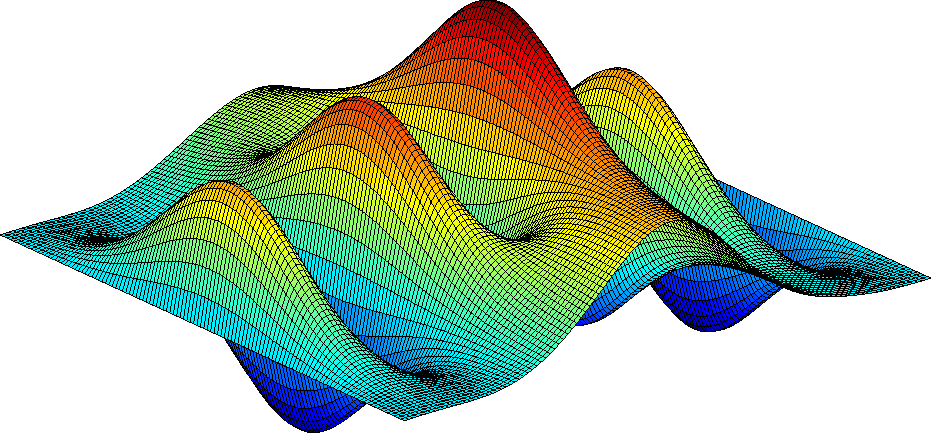
\includegraphics[width=6cm]{plotdata/plotgraphics3dsurf.png}}%
}

The key idea is now to identify several points in the image, and assign
\emph{both} their logical three-dimensional coordinates \emph{and} the
corresponding two-dimensional canvas coordinates in image coordinates. How?
Well, the three-dimensional coordinates are known to Matlab, it can display
them for you if you click somewhere into the image, compare
Figure~\ref{fig:plotgraphics3d} (left).


\begin{figure}
    \noindent
    \hbox to \linewidth{\hfill
        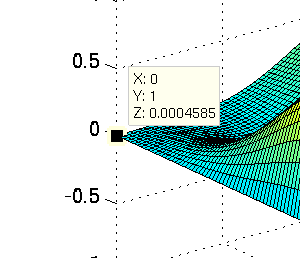
\includegraphics{plotdata/plotgraphics3dsurfmatlab.png}%
        \hfill
        \begin{minipage}[b][4cm][c]{2.6cm}%
        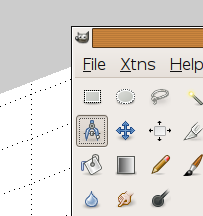
\includegraphics[width=\linewidth]{plotdata/plotgraphics_gimpmeasure.png}%
        \end{minipage}
        \hfill
    }
    \caption{Using Matlab to extract image coordinates (left) and Gimp to
             measure distances (right).}
        \label{fig:plotgraphics3d}
\end{figure}


The two-dimensional canvas coordinates need work; they need to be provided
relative to the \emph{lower left corner} of the image. I used |gimp| and
activated ``Points'' as units (lower left corner). The lower left corner now
displays the image coordinates in |pt| which is compatible with \PGFPlots{}. An
alternative to pointing onto coordinates is a measurement tool; compare
Figure~\ref{fig:plotgraphics3d} (right) for the ``Measure'' tool in |gimp|
which allows to compute the length of a line (in our case, the length of the
lower left corner to the point of interest).

I selected four points in the graphics and noted their 2d image coordinates and
their 3d logical coordinates as follows:
%
\begin{codeexample}[]
\begin{tikzpicture}
\begin{axis}[
    grid=both,minor tick num=1,
    xlabel=$x$,ylabel=$y$,
]
    \addplot3 graphics [
        points={% important
            (0,1,0) => (0,207-112)
            (1,0,0) => (446,207-133)
            (0.5546,0.5042,1.825) => (236,207)
            (0,0,0) => (194,207-202)
        },
    ] {plotdata/plotgraphics3dsurf.png};
\end{axis}
\end{tikzpicture}
\end{codeexample}
%
Here, the |points| key gets our collected coordinates as argument. It accepts a
sequence of maps of the form \meta{3d logical coordinate} | => | \meta{2d
canvas coordinate}. In our case, |(0,1,0)| has been found in the |.png| file at
|(0,207-112)|. Note that I introduced the difference since |gimp| counts from
the upper left, but \PGFPlots{} counts from the lower left.

Once these four point coordinates are gathered, we find Matlab's surface plot
in a \PGFPlots{} axis. You can modify any appearance options, including
different axis limits or further |\addplot| commands:
%
\begin{codeexample}[]
\begin{tikzpicture}
\begin{axis}[
    xmax=1.5,% extra limits
    grid=both,minor tick num=1,
    xlabel=$x$,ylabel=$y$,
]
    \addplot3 [surf] % 'surf': only used for legend
        graphics [
            points={
                (0,1,0) => (0,207-112)
                (1,0,0) => (446,207-133)
                (0.5546,0.5042,1.825) => (236,207)
                (0,0,0) => (194,207-202)
        },
    ] {plotdata/plotgraphics3dsurf.png};
        \addlegendentry{Graphics}

    \addplot3+ [only marks] coordinates {
        (0,1,0) (1,0,0)
        (0.5546,0.5042,1.825) (0,0,0)
    };
        \addlegendentry{Scatter}
\end{axis}
\end{tikzpicture}
\end{codeexample}
%
\noindent \PGFPlots{} uses the four input points to compute appropriate |x|,
|y| and |z| unit vectors (and the origin in graphics coordinates). These four
vectors (with two components each) can be computed as a result of a linear
system of size $8\times 8$, that is why you need to provide four input points
(each has two coordinates). \PGFPlots{} computes the unit vectors of the
imported graphics, and afterwards it rescales the result such that it fits into
the specified |width| and |height|. This rescaling respects the
|unit vector ratio| (more precisely, it uses |scale mode=scale uniformly|
instead of |scale mode=stretch to fill|). Consequently, the freedom to change
the view of a three-dimensional axis which contains a projected graphics is
considerably smaller than before. Surprisingly, you can still change axis
limits and |width| and |height| -- \PGFPlots{} will take care of a correct
display of your imported graphics. Since version~1.6, you can also change
|zmin| and/or |zmax| -- \PGFPlots{} will respect your changes as good as it
can.

Here is a further example. Suppose we are given the three-dimensional
visualization

{\setlength{\fboxsep}{0pt}%
\centering%
\fbox{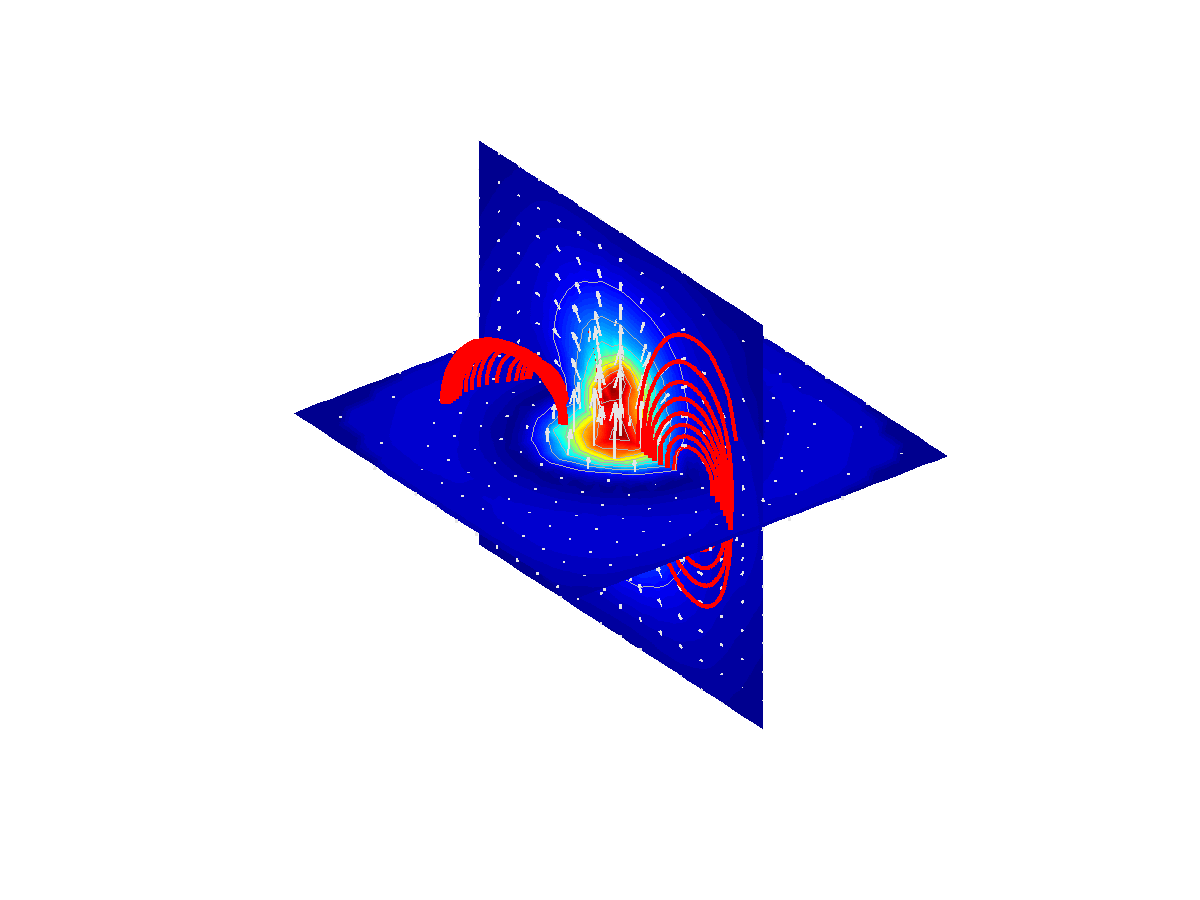
\includegraphics[width=6cm]{plotdata/risingdrop3d}}%
}

It has been generated by Matlab (I only added transparency to the background
with |gimp|). Besides advanced visualization techniques, it uses |axis equal|,
i.e.\@ |unit vector ratio=1 1 1|. As before, we need to identify four points,
each with its 3d logical coordinates (from Matlab) and the associated 2d canvas
coordinates relative to the lower left corner of the graphics (note that there
is a lot of white space around the graphics). Here is the output of \PGFPlots{}
when you import the resulting graphics:
%
\begin{codeexample}[]
\begin{tikzpicture}
\begin{axis}[
    grid=both,minor tick num=1,
    xlabel=$x$,ylabel=$y$,
    title={\centering
      Geometry provided by Sven Gro\ss, Bonn\\
      \url{http://www.igpm.rwth-aachen.de/DROPS}\\},
    title style={text width=6cm,font=\tiny},
]
    \addplot3 graphics [
        points={
            (-0.002625,0.002625,0) => (140,234)
            (0,0.00263,0.00263)    => (230,364)
            (0,-0.00263,-0.00263)  => (366,81)
            (0,-0.00263,0.00263)   => (366,276)
            (0.002625,0.002625,0.002625)
        },
    ] {plotdata/risingdrop3d.png};
\end{axis}
\end{tikzpicture}
\end{codeexample}
%
\noindent Note that I provided \emph{five} three-dimensional coordinates here,
but the last entry has no |=>| mapping to two-dimensional canvas coordinates.
Thus, it is only used to update the bounding box (see the reference manual for
the |points| key for details).

The example above leads to a relatively small image and much ``empty space''.
This is due to the |scale mode=scale uniformly| implementation of \PGFPlots{}:
it decided that the best way is to enlarge the involved axis limits. Here,
``best way'' means to satisfy |width|/|height| constraints combined with
minimally enlarged (never shrinked) axis limits. The remaining degrees of
freedom are |width|, |height|, and the axis limits. In our case, changing the
ratio between |width| and |height| improves the display:

\begin{codeexample}[]
\begin{tikzpicture}
\begin{axis}[
    height=8cm,width=7cm,% improve scaling manually
    grid=both,minor tick num=1,
    xlabel=$x$,ylabel=$y$,
    title={\centering
      Geometry provided by Sven Gro\ss, Bonn\\
      \url{http://www.igpm.rwth-aachen.de/DROPS}\\},
    title style={text width=6cm,font=\tiny},
]
    \addplot3 graphics [
        points={
            (-0.002625,0.002625,0) => (140,234)
            (0,0.00263,0.00263)    => (230,364)
            (0,-0.00263,-0.00263)  => (366,81)
            (0,-0.00263,0.00263)   => (366,276)
            (0.002625,0.002625,0.002625)
        },
    ] {plotdata/risingdrop3d.png};
\end{axis}
\end{tikzpicture}
\end{codeexample}
%
\noindent What happens is that \PGFPlots{} selects a \emph{single} scaling
factor which is applied to all units as they have been deduced from the
|points| key. This ensures that the imported graphics fits correctly into the
axis. In addition, \PGFPlots{} does its best to satisfy the remaining
constraints.

The complete description of how \PGFPlots{} scales the axis can be found in the
documentation for |scale mode=scale uniformly|. Here is just a brief summary:
\PGFPlots{} assumes that the prescribed |width| and |height| have to be
satisfied. To this end, it rescales the projected unit vectors (i.e.\@ the
space which is taken up for each unit in $x$, $y$, and $z$) and it can modify
the axis limits. In the default configuration |scale uniformly strategy=auto|,
\PGFPlots{} will \emph{never} shrink axis limits.


\paragraph{Compatibility remark:}

Note that the scaling capabilities have been improved for \PGFPlots{}
version~1.6. In previous versions, only
|scale uniformly strategy=change vertical limits| was available which lead to
clipped axes. In short: please consider writing |\pgfplotsset{compat=1.6}| or
newer into your document to benefit from the improved scaling. If you have
|\pgfplotsset{compat=1.5}| or older, the outcome for |\addplot3 graphics| will
be different.

We consider a third example which has been generated by the Matlab code
%
\begin{codeexample}[code only]
clear all
close all
seed = sum(clock)
rand('seed',seed);
X = rand(10,10,10);
data = smooth3(X,'box',5);
p1 = patch(isosurface(data,.5), ...
   'FaceColor','blue','EdgeColor','none');
p2 = patch(isocaps(data,.5), ...
    'FaceColor','interp','EdgeColor','none');
isonormals(data,p1)
daspect([1 2 2])
view(3); axis vis3d tight
camlight; lighting phong
% print -dpng plotgraphics3withaxis
axis off
print -dpng plotgraphics3
save  plotgraphics3.seed seed -ASCII % to reproduce the result
\end{codeexample}
%
\noindent I only added background transparency with |gimp| and got the following
graphics:

{\setlength{\fboxsep}{0pt}%
\centering%
\fbox{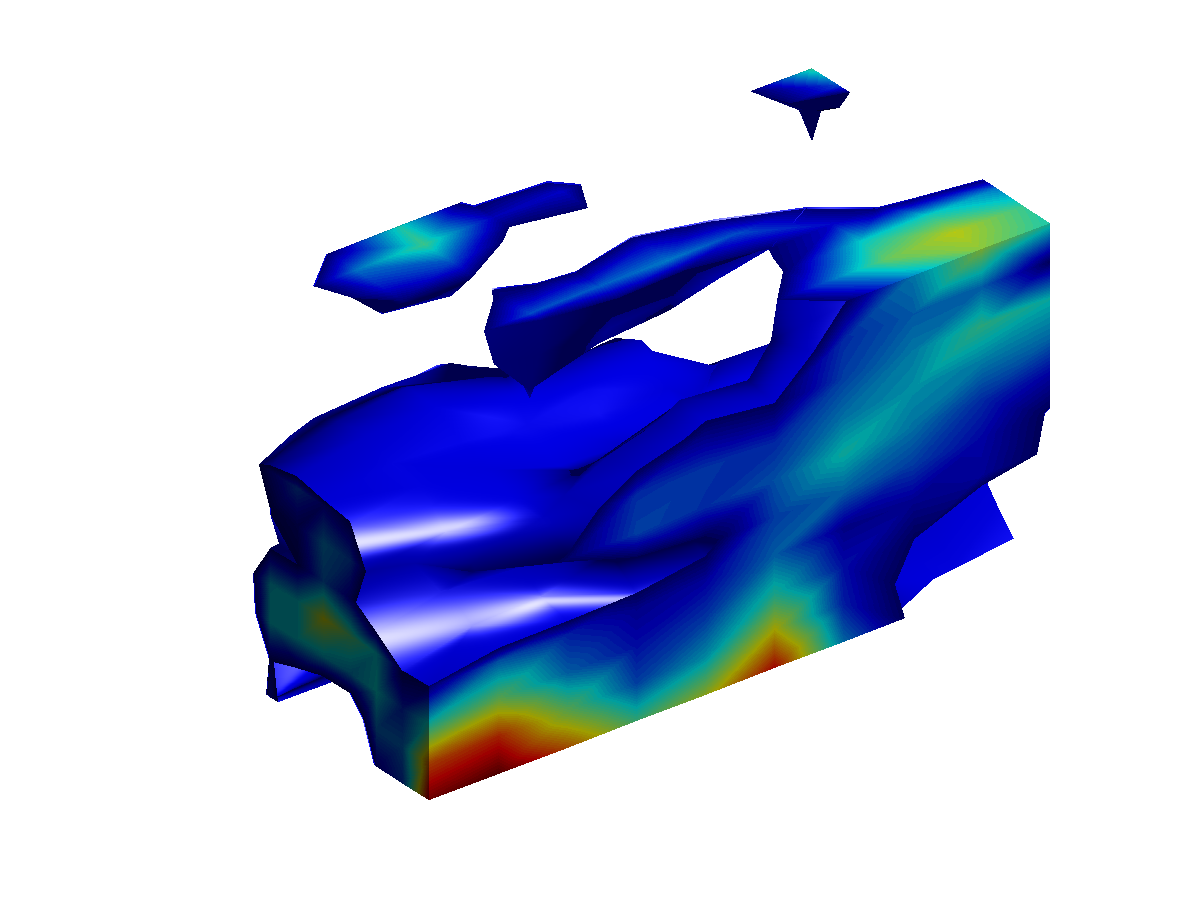
\includegraphics[width=6cm]{plotdata/plotgraphics3.png}}%
}

We proceed as before and collect four points, each with 3d logical coordinates
(by clicking into the Matlab figure) and their associated 2d canvas (graphics)
coordinates using the measure tool of gimp. The result is shown in the code
example below.
%
\begin{codeexample}[]
\begin{tikzpicture}
\begin{axis}[
    grid=both,minor tick num=1,
    xlabel=$x$,ylabel=$y$,
    3d box,
]
    \addplot3 graphics [
        points={
            (1,1,1)    => (205,48)
            (10,1,10)  => (503,324)
            (1,1,4.044)=> (206,102)
            (10,10,10) => (390,398)
        },
    ] {plotdata/plotgraphics3.png};
\end{axis}
\end{tikzpicture}
\end{codeexample}
%
\noindent Note that it has non-standard data aspect ratio which is respected by
\PGFPlots{} automatically.


\subsection*{External Three-Dimensional Graphics and Matlab}
\label{sec:plotgraphics3d:matlabscript}

\textit{An extension by Jürnjakob Dugge} \vskip\baselineskip

\noindent The procedure to map three-dimensional logical coordinates to
two-dimensional canvas coordinates is tedious.

Jürnjakob Dugge contributed a script which does most of the logic and your work
is reduced to a copy--paste job. With his permission, I post the contribution
here.

The idea is to start a simple script which \emph{records} mappings for any
coordinates which have been clicked by the user. It works as follows:
%
\begin{enumerate}
    \item Create the Matlab plot, say, using
        %
\begin{codeexample}[code only]
hist3(randn(10000,2)) % some random data
set(get(gca,'child'),'FaceColor','interp','CDataMode','auto'); % colors
% make sure the "print" paper format is the same as the screen paper format:
set(gcf,'PaperPositionMode','auto')
\end{codeexample}
        %
    \item Save the following code as |pgfplotscsconversion.m|:
        %
\begin{codeexample}[code only]
function pgfplotscsconversion

% Hook into the Data Cursor "click" event
h = datacursormode(gcf);
set(h,'UpdateFcn',@myupdatefcn,'SnapToDataVertex','off');
datacursormode on

% select four points in plot using mouse

% The function that gets called on each Data Cursor click
function [txt] = myupdatefcn(obj,event_obj)

% Get the screen resolution, in dots per inch
dpi = get(0,'ScreenPixelsPerInch');

% Get the click position in pixels, relative to the lower left of the
% screen
screen_location=get(0,'PointerLocation');

% Get the position of the plot window, relative to the lower left of
% the screen
figurePos = get(gcf,'Position');

% Get the data coordinates of the cursor
pos = get(event_obj,'Position');

% Format the data and figure coordinates. The factor "72.27/dpi" is
% necessary to convert from pixels to TeX points (72.27 poins per inch)
display(['(',num2str(pos(1)),',',num2str(pos(2)),',',num2str(pos(3)),') => (', ...
   num2str((screen_location(1)-figurePos(1))*72.27/dpi),',', ...
   num2str((screen_location(2)-figurePos(2))*72.27/dpi),')'])

% Format the tooltip display
txt = {['X: ',num2str(pos(1))],['Y: ',num2str(pos(2))],['Z: ',num2str(pos(3))]};
\end{codeexample}
        %
        Run |pgfplotscsconversion|, click on four points in your plot.
        Preferably select non-colinear points near the edges of the plot. Copy
        and paste the four lines that were written to the Matlab command
        window.

        Make sure that the first two points have different $X$ and $Y$ values
        on screen (i.e.\@ image canvas coordinates).
    \item Export the plot as an image
        %
\begin{codeexample}[code only]
axis off
print -dpng matlabout -r400 % PNG called "matlabout.png" with 400 dpi resolution
\end{codeexample}

        If you want to export vectors graphics, you should note that |pdf|
        output of Matlab is clumsy. It might be best to export to |eps| first,
        followed by a conversion from |eps| to |pdf|.

        \emph{If} you really want to use |pdf| output of Matlab, you may need
        to set the paper size to match the figure size by yourself, since the
        PDF driver does not automatically adjust the size:
        %
\begin{codeexample}[code only]
% It might be better to use print -depsc followed by epstopdf.
% Use this if you (really) want to use print -dpdf:
currentScreenUnits=get(gcf,'Units')     % Get current screen units
currentPaperUnits=get(gcf,'PaperUnits') % Get current paper units
set(gcf,'Units',currentPaperUnits)      % Set screen units to paper units
plotPosition=get(gcf,'Position')        % Get the figure position and size
set(gcf,'PaperSize',plotPosition(3:4))  % Set the paper size to the figure size
set(gcf,'Units',currentScreenUnits)     % Restore the screen units

print -dpdf matlabout      % PDF called "matlabout.pdf"
\end{codeexample}
        %
    \item Include the image in your \PGFPlots{} axis. If you selected points
        on the plot corners, your |xmin|, |xmax|, |ymin| and |ymax| should be
        set automatically, otherwise you may want to provide those yourself.
        Also, adjustments of |width| and |height| might be of interest to get
        the right vertical placement of the plot. Consider changing |zmin|
        and/or |zmax| to fit your needs (preferably only one of them;
        otherwise \PGFPlots{} may be unable to fix the |height|).
\end{enumerate}

This contribution is from

\noindent
\url{http://tex.stackexchange.com/questions/52987/3-dimensional-histogram-in-pgfplots} .


\subsection*{Summary: External Three-Dimensional Graphics}

As has been shown in the previous sections, \verbpdfref{\addplot3} |graphics|
allows to include three-dimensional graphics and \PGFPlots{} overlays a
flexible axis with all its power. The cost to do so is
%
\begin{enumerate}
    \item collect both logical three-dimensional coordinates \emph{and}
        image-internal two-dimensional coordinates for \emph{four points} of
        your graphics.

        In Matlab, this can be simplified by the tool mentioned on
        page~\pageref{sec:plotgraphics3d:matlabscript}.
    \item If your axes form a right-handed coordinate system, that is all. If
        not, also add |x dir=reverse| for any reversed axes.
\end{enumerate}

\noindent Consider the following list of you encounter problems while working
with \verbpdfref{\addplot3} |graphics|:
%
\begin{itemize}
    \item It must be possible to deduce the origin and the three
        (two-dimensional) unit vectors from the four provide |points|;
        otherwise the algorithm will fail.

        The algorithm should detect any deficiencies. However, if you
        encounter strange ``Dimension too large'' messages here, you can try
        other arguments in |points|. Take a look into your logfile, it will
        probably indicate the source of problems (or use the |debug| key).
    \item Ensure that the external graphics has an orthogonal axis. In fact,
        the axis may be skewed (just like a \PGFPlots{} axis can be created
        by means of custom |x|, |y|, and |z| vectors). However, the external
        image must not have perspective projection as this is unsupported by
        \PGFPlots{}. The |points| command needs to receive four points which
        belong to linearly independent position vectors.
    \item \PGFPlots{} uses the first two points to squeeze the graphics into
        the desired coordinates (which implies that they should not have the
        same canvas $X$ or $Y$ coordinates). It verifies that the remaining
        |points| arguments are projected correctly.
    \item The resulting scaling by means of |scale mode=scale uniformly| will
        try to satisfy all scaling constraints. You can change these
        constraints by modifying |width|, |height|, |xmin|, |xmax|, |ymin|,
        |ymax|, |zmin|, |zmax| and/or any combination of these parameters.
        See also |unit rescale keep size| which controls the flexibility of
        limit changes. There is also a key |scale uniformly strategy| which
        allows to select a different scaling strategy.
    \item The image should have a ``right-handed coordinate system'': you
        should be able to take your right hand, point your thumb in direction
        of the $x$-axis, your first finger in direction of~$y$, and your
        second finger in direction of the $z$-axis. If that is impossible,
        once of your axes is reversed and you need to communicate that to
        \PGFPlots{} explicitly by means of the |x dir=reverse| key (and its
        variants).
    \item Note that this feature has been verified with standard Cartesian
        axes only.
    \item There is a |debug| key to investigate what the algorithm is doing:
        %
        \begin{pgfplotskey}{plot graphics/debug=\mchoice{true,false,visual} (initially false)}
            If you provide |\addplot3 graphics[debug,points={...}]|,
            \PGFPlots{} will provide debug information onto your terminal and
            into the logfile. It will also generate extra files containing the
            determined unit vectors and the linear system used to derive them
            (one such file for every |\addplot3 graphics| statement, the
            filename will be the graphics file name and |.dat| appended).

            Without the |debug| key, only the logfile will contain brief
            information what \PGFPlots{} is doing behind the scenes.

            The choice \declaretext{true} activates log messages. The choice
            \declaretext{visual} activates log messages \emph{and} places some
            filled circles at the provided |points|. The choice
            \declaretext{false} disables all |debug| features.
        \end{pgfplotskey}
\end{itemize}
}


\subsection{Reading Coordinates From Files}

\begin{addplotoperation}[]{file}{\marg{name}}
\label{pgfplots:addplot:file}

    \paragraph{Deprecation note:}

    If you have data files, you should generally use |\addplot table|. The
    input type |\addplot file| is almost the same, but considerably less
    powerful. It is only kept for backwards compatibility.

    The |\addplot file| input mechanism is similar to the \Tikz{} command
    `|\addplot file|'. It is to be used like

\begin{codeexample}[code only]
\addplot file {datafile.dat};
\end{codeexample}
    %
    where \meta{name} is a text file with at least two columns which will be
    used as $x$- and $y$-coordinates. Lines starting with `|%|' or `|#|' are
    ignored. Such files are often generated by \textsc{gnuplot}:
    %
\begin{codeexample}[code only]
#Curve 0, 20 points
#x y type
0.00000 0.00000 i
0.52632 0.50235 i
1.05263 0.86873 i
1.57895 0.99997 i
...
9.47368 -0.04889 i
10.00000 -0.54402 i
\end{codeexample}
    %
    This listing has been copied from~\cite[Section~16.4]{tikz}.

    Plot file accepts one optional argument,

\begin{codeexample}[code only]
\addplot file [skip first] {datafile.dat};
\end{codeexample}

    \noindent which allows to skip over a non-comment header line. This allows
    to read the same input files as |\addplot table| by skipping over column names.
    Please note that comment lines do not count as lines here.

    The input method |\addplot file| can also read meta data for every coordinate.
    As already explained for |\addplot coordinates| (see above), meta data can be
    used to change colors or other style parameters for every marker
    separately. Now, if |point meta| is set to |explicit| or to
    |explicit symbolic| and the input method is |\addplot file|, one further element
    will be read from disk -- for every line. Meta data is always the last
    element which is read. See page~\pageref{pgfplots:scatter:src} for
    information and examples about per point meta data and
    page~\pageref{pgfplots:scatterclasses} for an application example using
    |scatter/classes|.

    Plot file is very similar to |\addplot table|: you can achieve the same effect
    with
    %
\begin{codeexample}[code only]
\addplot table [x index=0,y index=1,header=false] {datafile.dat};
\end{codeexample}
    %
    \noindent Due to its simplicity, |\addplot file| is slightly faster while
    |\addplot table| allows higher flexibility.

    Technical note: every opened file will be protocolled into your logfile.

    The file can contain |empty line|s to tell \PGFPlots{} that the function
    has jumps. To use it, simply insert an empty line (and ensure that you have
    |\pgfplotsset{compat=1.4}| or newer in your preamble). See the
    documentation of |empty line| for details.
\end{addplotoperation}

\begin{pgfplotskeylist}{%
    plot file/skip first=\mchoice{true,false} (initially false),
    plot file/ignore first=\mchoice{true,false} (initially false)%
}
    The two keys can be provided as arguments to
    |\addplot file[|\meta{options}|] |\marg{filename}|;| to skip the first
    non-comment entry in the file. They are equivalent. If you provide them in
    this context, the prefix |/pgfplots/plot file| can be omitted.
\end{pgfplotskeylist}
}


\section{About Options: Preliminaries}

\PGFPlots{} knows a whole lot of key--value options which can be (re)defined to
activate desired features or modified to apply some fine-tuning.

A key usually has a value (like a number, a string, or perhaps some macro
code). You can assign values to keys (``set keys'') in many places in a
\LaTeX{} document. The value will remain effective until it is changed or until
the current \TeX{} scope ends (which happens after a closing curly brace `|}|',
after |\end|\marg{name} or, for example, after |\addplot|).

\noindent Most keys can be used like
%
\begin{codeexample}[code only]
\begin{tikzpicture}
\begin{axis}[key=value,key2=value2] % axis-wide keys
...
\end{axis}
\end{tikzpicture}
\end{codeexample}
%
\noindent which changes them for the complete axis. A |key| in this context can
be any option defined in this manual, no matter if it has the |/pgfplots/| or
the |/tikz/| key prefix. Note that key prefixes can be omitted in almost all
cases.

A value can usually be provided without curly braces. For example, if the
manual contains something like `|xmin=|\marg{$x$-coordinate}', you can safely
skip the curly braces. The curly braces are mandatory if values contain
something which would otherwise confuse the key setup (for example an equal
sign `|=|' or a comma `|,|').

Some keys can be changed individually for each plot:
%
\begin{codeexample}[code only]
\begin{tikzpicture}
    \begin{axis}
        % keys valid for single plots:
        \addplot ... ;                          % uses the "cycle list" to determine keys
        \addplot [key=value,key2=value2] ... ;  % uses the provided keys (not the "cycle list")
        \addplot+ [key=value,key2=value2] ... ; % appends something to the "cycle list"
    \end{axis}
\end{tikzpicture}
\end{codeexample}

Besides these two possibilities, it is also possible to work with document-wide
keys:
%
\begin{codeexample}[code only]
\chapter{My Chapter}
\pgfplotsset{
    key=value,
    key2=value2,
}
This chapter has a common key configuration:
\begin{tikzpicture}
    \begin{axis}% uses the key config from above
    ...
    \end{axis}
\end{tikzpicture}
\end{codeexample}
%
\noindent In the example above, the |\pgfplotsset| command changes keys. The
changes are permanent and will be used until
%
\begin{itemize}
    \item you redefine them or
    \item the current environment (like |\end{figure}|) is ended or
    \item \TeX{} encounters a closing brace `|}|'.
\end{itemize}
%
This includes document-wide preamble configurations like
%
\begin{codeexample}[code only]
\documentclass{article}

\usepackage{pgfplots}
\pgfplotsset{
    xticklabel={$\mathsf{\pgfmathprintnumber{\tick}}$},
    every axis/.append style={
        font=\sffamily,
    },
}
...
\end{codeexample}

The basic engine to manage key--value pairs is |pgfkeys| which is part of
\pgfname{}. This engine always has a key name and a key ``path'', which is
somehow similar to file name and directory of files. The common ``directory''
(key path) of \PGFPlots{} is `|/pgfplots/|'. Although the key definitions below
provide this full path, it is always (well, almost always) safe to skip this
prefix -- \PGFPlots{} uses it automatically. The same holds for the prefixes
`|/tikz/|' which are common for all \Tikz{} drawing options and `|/pgf/|' which
are for the (more or less) low-level commands of \pgfname{}. All these prefixes
can be omitted.

One important concept is the concept of \emph{styles}. A style is a key which
contains one or more other keys. It can be redefined or modified until it is
actually used by the internal routines. Each single component of \Tikz{} and
\PGFPlots{} can be configured with styles.

For example,
%
\begin{codeexample}[code only]
\pgfplotsset{legend style={line width=1pt}}
\end{codeexample}
%
\noindent sets the line width for every legend to |1pt| by appending
`|line width=1pt|' to the existing style for legends.

There are keys like |legend style|, |ticklabel style|, and |label style| which
allow to modify the predefined styles (in this case the styles for legends,
ticklabels and axis labels, respectively). They are, in general, equivalent to
a \meta{style name}|/.append style={}| command (the only difference is that the
|/.append style| thing is a little bit longer). There is also the possibility
to define a new style (or to overwrite an already existing one) using
|/.style={}|.

There are several other styles predefined to modify the appearance, see
Section~\ref{sec:styles}.

\begin{command}{\pgfplotsset\marg{key-value-list}}
    Defines or sets all options in \meta{key-value-list}. The
    \meta{key-value-list} can contain any of the options in this manual which
    have the prefix |/pgfplots/| (however, you do not need to type that
    prefix).

    Inside of \meta{key-value-list}, the prefixes `|/pgfplots/|' which are
    commonly presented in this manual can be omitted (they are checked
    automatically).

    This command can be used to define default options for the complete
    document or a part of the document. For example,
    %
\begin{codeexample}[code only]
\pgfplotsset{
    cycle list={
        {red, mark=*},          {blue,mark=*},
        {red, mark=x},          {blue,mark=x},
        {red, mark=square*},    {blue,mark=square*},
        {red, mark=triangle*},  {blue,mark=triangle*},
        {red, mark=diamond*},   {blue,mark=diamond*},
        {red, mark=pentagon*},  {blue,mark=pentagon*}
    },
    legend style={
        at={(0.5,-0.2)},
        anchor=north,
        legend columns=2,
        cells={anchor=west},
        font=\footnotesize,
        rounded corners=2pt,
    },
    xlabel=$x$,
    ylabel=$f(x)$,
}
\end{codeexample}
    %
    can be used to set document-wise styles for line specifications, the
    legends' style and axis labels. The settings remain in effect until the end
    of the current environment (like |\end{figure}|) or until you redefine them
    or until the next closing curly brace `|}|' (whatever comes first).

    You can also define new styles (collections of key--value pairs) with
    |/.style| and |/.append style|.
    %
\begin{codeexample}[code only]
\pgfplotsset{
    My Style 1/.style={xlabel=$x$, legend entries={1,2,3} },
    My Style 2/.style={xlabel=$X$, legend entries={4,5,6} }
}
\end{codeexample}
    %
    The |/.style| and |/.append style| key handlers are described in
    Section~\ref{sec:styles} in more detail.
\end{command}

\begin{handler}{{.code}=\marg{\TeX{} code}}
    Occasionally, the \PGFPlots{} user interface offers to replace parts of its
    routines. This is accomplished using so called ``code keys''. What it means
    is to replace the original key and its behavior with new \meta{\TeX{}
    code}. Inside of \meta{\TeX{} code}, any command can be used. Furthermore,
    the |#1| pattern will be the argument provided to the key.

\begin{codeexample}[]
\pgfplotsset{
    My Code/.code={I've been invoked with `#1'}}
\pgfplotsset{My Code={this here}}
\end{codeexample}
    %
    The example defines a (new) key named |My Code|. Essentially, it is nothing
    else but a |\newcommand|, plugged into the key--value interface. The second
    statement ``invokes'' the code key.
\end{handler}

\begin{handler}{{.code 2 args}=\marg{\TeX{} code}}
    As |/.code|, but this handler defines a key which accepts two arguments.
    When the so defined key is used, the two arguments are available as |#1|
    and |#2|.
\end{handler}

\begin{handler}{{.cd}}
    Each key has a fully qualified name with a (long) prefix, like
    |/pgfplots/xmin|. However, if the ``current directory'' is |/pgfplots|, it
    suffices to write just |xmin|. The |/.cd| key handler changes the ``current
    directory'' in this way.

    The prefixes |/tikz/| and |/pgfplots/| are checked automatically for any
    argument provided to |\begin{axis}|\oarg{options} or |\addplot|. So, you
    won't need to worry about them, just omit them -- and look closer in case
    the package doesn't identify the option.
\end{handler}


\subsection{\textsc{PGFPlots} and \Tikz{} Options}

This section is more or less technical and can be skipped unless one really
wants to know more about this topic.

\Tikz{} options and \PGFPlots{} options can be mixed inside of the axis
arguments and in any of the associated styles. For example,
%
\begin{codeexample}[code only]
\pgfplotsset{every axis legend/.append style={
    legend columns=3,font=\Large},
}
\end{codeexample}
%
\noindent assigns the `|legend columns|' option (a \PGFPlots{} option) and uses
`|font|' for drawing the legend (a \Tikz{} option). The point is:
|legend columns| needs to be known \emph{before} the legend is typeset whereas
|font| needs to be active when the legend is typeset. \PGFPlots{} sorts out any
key dependencies automatically:

The axis environments will process any known \PGFPlots{} options, and all
`|every|' styles will be parsed for \PGFPlots{} options. Every unknown option
is assumed to be a \Tikz{} option and will be forwarded to the associated
\Tikz{} drawing commands. For example, the `|font=\Large|' above will be used
as argument to the legend matrix, and the `|font=\Large|' argument in
%
\begin{codeexample}[code only]
\pgfplotsset{every axis label/.append style={
    ylabel=Error,xlabel=Dof,font=\Large},
}
\end{codeexample}
%
will be used in the nodes for axis labels (but not the axis title, for example).

It is an error if you assign incompatible options to axis labels, for example
`|xmin|' and `|xmax|' can't be set inside of `|every axis label|'.


\section{Two Dimensional Plot Types}

{%
\tikzset{external/figure name/.add={}{twodim_}}

\PGFPlots{} supports several two-dimensional line plots like piecewise linear
line plots, piecewise constant plots, smoothed plots, bar plots and comb plots.
Most of them use the \PGF{} plot handler library directly, see
\cite[Section~18.8]{tikz}.

Plot types are part of the plot style, so they are set with options. Most of
the basic 2d plot types are part of \Tikz{}, see \cite[Section~18.8]{tikz}, and
are probably known to users of \Tikz{}. They are documented here as well.


\subsection{Linear Plots}

\begin{plottype}{sharp plot}
    Linear (`sharp') plots are the default. Point coordinates are simply
    connected by straight lines.
\begin{codeexample}[]
\begin{tikzpicture}
\begin{axis}
    \addplot+ [
        sharp plot,
    ] coordinates {
        (0,0) (1,2) (2,3)
    };
\end{axis}
\end{tikzpicture}
\end{codeexample}

    The `|+|' here means to use the normal plot cycle list and append
    `|sharp plot|' to its option list.
\end{plottype}


\subsection{Smooth Plots}

\begin{plottype}{smooth}
    Smooth plots interpolate smoothly between successive points.
\begin{codeexample}[]
\begin{tikzpicture}
\begin{axis}
    \addplot+ [
        smooth,
    ] coordinates {
        (0,0) (1,2) (2,3)
    };
\end{axis}
\end{tikzpicture}
\end{codeexample}
\end{plottype}

As described in~\cite{tikz} in all detail, this plot handler results in a
``smooth'' outline. However, it ``not very intelligent'' (compare~\cite{tikz})
and is unrelated to common plot-based interpolation schemes.

\begin{key}{/tikz/tension=\marg{tension} (initially 0.55)}
    A parameter which controls how the remaining degrees of freedom are fixed:
    it controls the smoothing effect. Higher values results in more ``rounded''
    corners whereas low values result in sharp corners.

    Please refer to~\cite{tikz} for details.
\end{key}


\subsection{Constant Plots}

Constant plots draw lines parallel to the $x$-axis to connect coordinates. The
discontinuous edges may be drawn or not, and marks may be placed on left or
right ends.

\begin{plottype}{const plot}
    Connects all points with horizontal and vertical lines. Marks are placed
    left-handed on horizontal line segments, causing the plot to be right-sided
    continuous at all data points.

\begin{codeexample}[]
\begin{tikzpicture}
\begin{axis}
    \addplot+ [
        const plot,
    ] coordinates {
        (0,0.1)    (0.1,0.15)  (0.2,0.5)   (0.3,0.62)
        (0.4,0.56) (0.5,0.58)  (0.6,0.65)  (0.7,0.6)
        (0.8,0.58) (0.9,0.55)  (1,0.52)
    };
\end{axis}
\end{tikzpicture}
\end{codeexample}


\begin{codeexample}[]
\begin{tikzpicture}
\begin{axis}[ymin=0,ymax=1,enlargelimits=false]
    \addplot [
        const plot,
        fill=blue,
        draw=black,
    ] coordinates {
        (0,0.1)    (0.1,0.15)  (0.2,0.5)   (0.3,0.62)
        (0.4,0.56) (0.5,0.58)  (0.6,0.65)  (0.7,0.6)
        (0.8,0.58) (0.9,0.55)  (1,0.52)
    }
        \closedcycle
    ;
\end{axis}
\end{tikzpicture}
\end{codeexample}
\end{plottype}

\begin{plottype}{const plot mark left}
    An alias for `|const plot|'.
\end{plottype}

\begin{plottype}{const plot mark right}
    A variant which places marks on the right of each line segment, causing
    plots to be left-sided continuous at the given coordinates.
    %
\begin{codeexample}[]
\begin{tikzpicture}
\begin{axis}
    \addplot+ [
        const plot mark right,
    ] coordinates {
        (0,0.1)    (0.1,0.15)  (0.2,0.5)   (0.3,0.62)
        (0.4,0.56) (0.5,0.58)  (0.6,0.65)  (0.7,0.6)
        (0.8,0.58) (0.9,0.55)  (1,0.52)
    };
\end{axis}
\end{tikzpicture}
\end{codeexample}
\end{plottype}

\begin{plottype}{const plot mark mid}
    A variant which places marks in the middle of each line segment, causing
    plots to be symmetric around its data points.
    %
\begin{codeexample}[]
\begin{tikzpicture}
\begin{axis}
    \addplot+ [
        const plot mark mid,
    ] coordinates {
        (0,0.1)    (0.1,0.15)  (0.2,0.5)   (0.3,0.62)
        (0.4,0.56) (0.5,0.58)  (0.6,0.65)  (0.7,0.6)
        (0.8,0.58) (0.9,0.55)  (1,0.52)
    };
\end{axis}
\end{tikzpicture}
\end{codeexample}
    %
    Note that ``symmetric'' is only true for constant mesh width: if the
    $x$-distances between adjacent data points differ, |const plot mark mid|
    will produce vertical lines in the middle between each pair of consecutive
    points.
\end{plottype}

\begin{plottype}{jump mark left}
    A variant of `|const plot mark left|' which does not draw vertical lines.
    %
\begin{codeexample}[]
\begin{tikzpicture}
\begin{axis}[samples=8]
    \addplot+ [
        jump mark left,
        domain=-5:0,
    ] {4*x^2 - 5};

    \addplot+ [
        jump mark right,
        domain=-5:0,
    ] {0.7*x^3 + 50};
\end{axis}
\end{tikzpicture}
\end{codeexample}
\end{plottype}

\begin{plottype}{jump mark right}
    A variant of `|const plot mark right|' which does not draw vertical lines.
\end{plottype}

\begin{plottype}{jump mark mid}
    A variant of `|const plot mark mid|' which does not draw vertical lines.
    %
\begin{codeexample}[]
\begin{tikzpicture}
\begin{axis}
    \addplot+ [
        jump mark mid,
    ] coordinates {
        (0,0.1)    (0.1,0.15)  (0.2,0.5)   (0.3,0.62)
        (0.4,0.56) (0.5,0.58)  (0.6,0.65)  (0.7,0.6)
        (0.8,0.58) (0.9,0.55)  (1,0.52)
    };
\end{axis}
\end{tikzpicture}
\end{codeexample}
\end{plottype}


\subsection{Bar Plots}

Bar plots place horizontal or vertical bars at coordinates. Multiple bar plots
in one axis can be stacked on top of each other or aligned next to each other.

\begin{plottype}{xbar}
    Places horizontal bars between the $(y=0)$ line and each coordinate.

    This option is used on a per-plot basis and configures only the
    visualization of coordinates. The figure-wide style |/pgfplots/xbar| also
    sets reasonable options for ticks, legends and multiple plots.
    %
\begin{codeexample}[]
\begin{tikzpicture}
\begin{axis}
    \addplot+ [
        xbar,
    ] coordinates {
        (4,0) (1,1) (2,2)
        (5,3) (6,4) (1,5)
    };
\end{axis}
\end{tikzpicture}
\end{codeexample}
    %
    Bars are centered at plot coordinates with width |bar width|. Using bar
    plots usually means more than just a different way of how to connect
    coordinates, for example to draw ticks outside of the axis, change the
    legend's appearance or introduce shifts if multiple |\addplot| commands
    appear.

    There is a pre-configured style for |xbar| which is installed automatically
    if you provide |xbar| as argument to the axis environment which provides
    this functionality.
    %
% \usetikzlibrary{patterns}
\begin{codeexample}[]
\begin{tikzpicture}
\begin{axis}[xbar,enlargelimits=0.15]
    \addplot [draw=blue,
        pattern=horizontal lines light blue,
    ] coordinates {
        (10,5) (15,10) (5,15) (24,20) (30,25)
    };
    \addplot [draw=black,
        pattern=horizontal lines dark blue,
    ] coordinates {
        (3,5) (5,10) (15,15) (20,20) (35,25)
    };
\end{axis}
\end{tikzpicture}
\end{codeexample}
    %
    Here |xbar| yields |/pgfplots/xbar| because it is an argument to the axis,
    not to a single plot.

    For bar plots, it is quite common to provide textual coordinates or even
    descriptive nodes near the bars. This can be implemented using the keys
    |symbolic y coords| and |nodes near coords|, respectively:
    %
\begin{codeexample}[]
\begin{tikzpicture}
    \begin{axis}[
        xbar, xmin=0,
        width=12cm, height=3.5cm, enlarge y limits=0.5,
        xlabel={\#participants},
        symbolic y coords={no,yes},
        ytick=data,
        nodes near coords, nodes near coords align={horizontal},
    ]
        \addplot coordinates {(3,no) (7,yes)};
    \end{axis}
\end{tikzpicture}
\end{codeexample}
    %
    The |symbolic y coords| defines a dictionary of accepted coordinates which
    are then expected in $y$-coordinates and the |nodes near coords| key
    displays values as extra nodes (see their reference documentations for
    details). The example employs |enlarge y limits| in order to get some more
    free space since the default spacing is not always appropriate for bar
    plots.

    Note that it might be quite important to include |xmin=0| explicitly as in
    the example above. Without it, the lower bound will be used:
    %
\begin{codeexample}[]
\begin{tikzpicture}
    \begin{axis}[
        title=Uses lowest $x$ coords for xmin,
        xbar,
        width=12cm, height=3.5cm, enlarge y limits=0.5,
        xlabel={\#participants},
        symbolic y coords={no,yes},
        ytick=data,
        nodes near coords, nodes near coords align={horizontal},
      ]
        \addplot coordinates {(1,no) (9,yes)};
    \end{axis}
\end{tikzpicture}
\end{codeexample}

    Besides line, fill, and color styles, bars can be configured with
    |bar width| and |bar shift|, see below.
\end{plottype}

\begin{stylekey}{/pgfplots/xbar=\marg{shift for multiple plots} (default 2pt)}
    This style sets |/tikz/xbar| \emph{and} some commonly used options
    concerning horizontal bars for the complete axis. This is automatically
    done if you provide |xbar| as argument to an axis argument, see above.

    The |xbar| style defines shifts if multiple plots are placed into one axis.
    It draws bars adjacent to each other, separated by \meta{shift for multiple
    plots}. Furthermore, it sets the style |bar cycle list| and sets tick and
    legend appearance options.

    The style is defined as follows.
    %
\begin{codeexample}[code only]
\pgfplotsset{
    /pgfplots/xbar/.style={
        /tikz/xbar,
        bar cycle list,
        tick align=outside,
        xbar legend,
        /pgfplots/bar shift auto={#1},
    },
}
\end{codeexample}

    \begin{pgfplotskey}{bar shift auto=\marg{shift for multiple plots} (default 2pt)}
        The formula for |bar shift| assigns shifts dependent on the total
        number of plots and the current plot's number. It is designed to fill a
        total width of $n \cdot $|bar width|$ + (n-1) \cdot $\meta{shift for
        multiple plots}. The $0.5$ compensates for centering.

        The style is defined as
        %
\begin{codeexample}[code only]
\pgfplotsset{
    /pgfplots/bar shift auto/.style={
        /pgf/bar shift={%
            % total width = n*w + (n-1)*skip
            % -> subtract half for centering
            -0.5*(\numplotsofactualtype*\pgfplotbarwidth + (\numplotsofactualtype-1)*(#1)) +
            % the '0.5*w' is for centering
            (.5+\plotnumofactualtype)*\pgfplotbarwidth + \plotnumofactualtype*(#1)},
    },
}
\end{codeexample}
    \end{pgfplotskey}
\end{stylekey}

\begin{plottype}{ybar}
    Like |xbar|, this option generates bar plots. It draws vertical bars
    between the ($x=0$) line and each input coordinate.
    %
\begin{codeexample}[]
\begin{tikzpicture}
\begin{axis}
    \addplot+ [
        ybar,
    ] coordinates {
        (0,3) (1,2) (2,4) (3,1) (4,2)
    };
\end{axis}
\end{tikzpicture}
\end{codeexample}
    %
    The example above simply changes how input coordinates shall be visualized.
    As mentioned for |xbar|, one usually needs modified legends and shifts for
    multiple bars in the same axis.

    There is a predefined style which installs these customizations when
    provided to the axis environment:
    %
\begin{codeexample}[]
\begin{tikzpicture}
\begin{axis}[
    x tick label style={
        /pgf/number format/1000 sep=},
    ylabel=Population,
    enlargelimits=0.15,
    legend style={at={(0.5,-0.15)},
        anchor=north,legend columns=-1},
    ybar,
    bar width=7pt,
]
    \addplot coordinates {
        (1930,50e6) (1940,33e6)
        (1950,40e6) (1960,50e6) (1970,70e6)
    };
    \addplot coordinates {
        (1930,38e6) (1940,42e6)
        (1950,43e6) (1960,45e6) (1970,65e6)
    };
    \addplot coordinates {
        (1930,15e6) (1940,12e6)
        (1950,13e6) (1960,25e6) (1970,35e6)
    };
    \addplot [red,line legend,
        sharp plot,update limits=false,
    ] coordinates { (1910,4.3e7) (1990,4.3e7) }
        node [above] at (1950,4.3e7) {Houses};

    \legend{Far,Near,Here,Annot}
\end{axis}
\end{tikzpicture}
\end{codeexample}
    %
    Here, |ybar| yields |/pgfplots/ybar| because it is an argument to the axis,
    not to a single plot. The style affects the first three |\addplot|
    commands. Note that it shifts them horizontally around the plot
    coordinates. The fourth |\addplot| command is some kind of annotation which
    doesn't |update limits|.

    The |ybar| style can be combined with |symbolic x coords| in a similar way
    as described for |xbar|:
    %
\begin{codeexample}[]
\begin{tikzpicture}
\begin{axis}[
    ybar,
    enlargelimits=0.15,
    legend style={at={(0.5,-0.15)},
    anchor=north,legend columns=-1},
    ylabel={\#participants},
    symbolic x coords={tool8,tool9,tool10},
    xtick=data,
    nodes near coords,
    nodes near coords align={vertical},
]
\addplot coordinates {(tool8,7) (tool9,9) (tool10,4)};
\addplot coordinates {(tool8,4) (tool9,4) (tool10,4)};
\addplot coordinates {(tool8,1) (tool9,1) (tool10,1)};
    \legend{used,understood,not understood}
\end{axis}
\end{tikzpicture}
\end{codeexample}

    As for |xbar|, the bar width and shift can be configured with |bar width|
    and |bar shift|. However, the bar shift is better provided as argument to
    |/pgfplots/ybar| since this style will overwrite the bar shift. Thus,
    prefer |/pgfplots/ybar=4pt| to set the bar shift.

    Sometimes it is useful to write the $y$ values directly near the bars. This
    can be realized using the |nodes near coords| method:
    %
\begin{codeexample}[]
\begin{tikzpicture}
\begin{axis}[
    x tick label style={
        /pgf/number format/1000 sep=},
    ylabel=Population,
    enlargelimits=0.15,
    legend style={at={(0.5,-0.15)},
        anchor=north,legend columns=-1},
    ybar=5pt,% configures `bar shift'
    bar width=9pt,
    nodes near coords,
    point meta=y *10^-7, % the displayed number
]
    \addplot coordinates {
        (1930,50e6) (1940,33e6)
        (1950,40e6) (1960,50e6) (1970,70e6)
    };
    \addplot coordinates {
        (1930,38e6) (1940,42e6)
        (1950,43e6) (1960,45e6) (1970,65e6)
    };
    \legend{Far,Near}
\end{axis}
\end{tikzpicture}
\end{codeexample}

    Any support style changes are possible, of course. A useful example for bar
    plots might be to use rotated tick labels:
    %
\begin{codeexample}[]
\begin{tikzpicture}
\begin{axis}[
    ybar,
    enlargelimits=0.15,
    legend style={at={(0.5,-0.2)},
    anchor=north,legend columns=-1},
    ylabel={\#participants},
    symbolic x coords={excellent,good,neutral,%
        not good,poor},
    xtick=data,
    nodes near coords,
    nodes near coords align={vertical},
    x tick label style={rotate=45,anchor=east},
]
    \addplot coordinates {
        (excellent,0) (good,8) (neutral,2)
        (not good,0) (poor,0)
    };
\end{axis}
\end{tikzpicture}
\end{codeexample}
\end{plottype}

\begin{stylekey}{/pgfplots/ybar=\marg{shift for multiple plots} (default 2pt)}
    As |/pgfplots/xbar|, this style sets the |/tikz/ybar| option to draw
    vertical bars, but it also provides commonly used options for vertical
    bars.

    If you supply |ybar| to an axis environment, |/pgfplots/ybar| will be
    chosen instead of |/tikz/ybar|.

    It changes the legend, draws ticks outside of the axis lines and draws
    multiple |\addplot| arguments adjacent to each other; block-centered at the
    $x$-coordinate and separated by \meta{shift for multiple plots}. It will
    also install the |bar shift| for |every node near coord|. Furthermore, it
    installs the style |bar cycle list|. It is defined similarly to
    |/pgfplots/xbar|.
\end{stylekey}

\begin{pgfplotskey}{bar cycle list}
    A style which installs cycle lists for multiple bar plots.
    %
\begin{codeexample}[code only]
\pgfplotsset{
    /pgfplots/bar cycle list/.style={/pgfplots/cycle list={
            {blue,fill=blue!30!white,mark=none},
            {red,fill=red!30!white,mark=none},
            {brown!60!black,fill=brown!30!white,mark=none},
            {black,fill=gray,mark=none},
        },
    },
}
\end{codeexample}
\end{pgfplotskey}

\begin{key}{/pgf/bar width=\marg{dimension or unit} (initially 10pt)}
    Configures the width used by |xbar| and |ybar|. It is accepted to provide
    mathematical expressions.

    As of \PGFPlots{} 1.7, it is allows to provide a \emph{unit} as
    |bar width|. In this case, the |bar width| will be interpreted as axis unit:
    %
\begin{codeexample}[]
\begin{tikzpicture}
\begin{axis}[
    xbar=0pt,% space of 0pt between adjacent bars
    bar width=2,
    width=7cm,
    height=12cm,
    minor y tick num=4,
    ytick=data,
    enlargelimits=0.15,
]
    \addplot coordinates {
        (10,5) (15,10) (5,15) (24,20) (30,25)
    };
    \addplot coordinates {
        (3,5) (5,10) (15,15) (20,20) (35,25)
    };
\end{axis}
\end{tikzpicture}
\end{codeexample}
    %
    In order to interpret arguments as units, you have to write
    |\pgfplotsset{compat=1.7}| (or newer) into your preamble. Older versions
    will implicitly append the |pt| suffix if the argument is no dimension.

    \begin{command}{\pgfplotbarwidth}
        A mathematical expression which results in the fully computed value of
        |bar width| (i.e.\@ it includes any unit computations).
    \end{command}

    Note that you may need to |enlargelimits| in order to see the complete bar
    -- \PGFPlots{} will not automatically update the axis limits to respect
    |bar width|.
\end{key}

\begin{key}{/pgf/bar shift=\marg{dimension or unit} (initially 0pt)}
    Configures a shift for |xbar| and |ybar|. Use |bar shift| together with
    |bar width| to draw multiple bar plots into the same axis. It is accepted
    to provide mathematical expressions.

    As of \PGFPlots{}~1.7, it is allows to provide an \emph{unit} as
    |bar shift|. In this case, the |bar shift| will be interpreted as axis unit.

    \begin{command}{\pgfplotbarshift}
        A mathematical expression which results in the fully computed value of
        |bar shift| (i.e.\@ it includes any unit computations).
    \end{command}

    Note that you may need to |enlargelimits| in order to see the complete bar
    -- \PGFPlots{} will not automatically update the axis limits to respect
    |bar shift|.
\end{key}

\begin{pgfplotskey}{bar direction=\mchoice{auto,x,y} (initially auto)}
    If \PGFPlots{} encounters a value |bar width=1| (i.e.\@ \emph{without}
    dimension like |1pt|), it attempts to evaluate the bar's direction.

    The default configuration \declareandlabel{auto} assumes that you write
    something like |ybar,bar width=1|. In this case, it is clear that you have
    a $y$ bar and \PGFPlots{} assumes |bar direction=y|.

    However, this context information is unavailable. In this case, you can use
    the choice \declaretext{x} if \PGFPlots{} in unaware that it works on an
    |xbar| plot or \declaretext{y} if \PGFPlots{} is unaware that you meant an
    |ybar| plot.
\end{pgfplotskey}

\begin{plottype}{ybar interval}
    This plot type produces vertical bars with width (and shift) relatively to
    intervals of coordinates.

    There is one conceptional difference when working with intervals: an
    interval is defined by \emph{two} coordinates. Since |ybar| has one value
    for each interval, the $i$th bar is defined by
    %
    \begin{enumerate}
        \item the $y$ value of the $i$th coordinates,
        \item the $x$ value of the $i$th coordinate as left interval
            boundary,
        \item the $x$ value of the $(i+1)$th coordinate as right interval
            boundary.
    \end{enumerate}
    %
    Consequently, there is \emph{one coordinate too much}: the last coordinate
    will \emph{only} be used to determine the interval width; its $y$ value
    doesn't influence the bar appearance.

    It is installed on a per-plot basis and configures \emph{only} the
    visualization of coordinates. See the style |/pgfplots/ybar interval| which
    configures the appearance of the complete figure.
    %
\begin{codeexample}[]
\begin{tikzpicture}
\begin{axis}
    \addplot+ [
        ybar interval,
    ] coordinates {
        (0,2) (0.1,1) (0.3,0.5) (0.35,4) (0.5,3)
        (0.6,2) (0.7,1.5) (1,1.5)
    };
\end{axis}
\end{tikzpicture}
\end{codeexample}

\begin{codeexample}[]
\begin{tikzpicture}
\begin{axis}[ybar interval,
    xtick=data,
    xticklabel interval boundaries,
    x tick label style={
        rotate=90,
        anchor=east,
    },
]
    \addplot coordinates {
        (0,2) (0.1,1) (0.3,0.5) (0.35,4) (0.5,3)
        (0.6,2) (0.7,1.5) (1,1.5)
    };
\end{axis}
\end{tikzpicture}
\end{codeexample}

\begin{codeexample}[]
\begin{tikzpicture}
\begin{axis}[
    x tick label style={
        /pgf/number format/1000 sep=},
    ylabel=Population,
    enlargelimits=0.05,
    legend style={at={(0.5,-0.15)},
    anchor=north,legend columns=-1},
    ybar interval=0.7,
]
    \addplot coordinates {
        (1930,50e6) (1940,33e6)
        (1950,40e6) (1960,50e6) (1970,70e6)
    };
    \addplot coordinates {
        (1930,38e6) (1940,42e6)
        (1950,43e6) (1960,45e6) (1970,65e6)
    };
    \addplot coordinates {
        (1930,15e6) (1940,12e6)
        (1950,13e6) (1960,25e6) (1970,35e6)
    };
    \legend{Far,Near,Here}
\end{axis}
\end{tikzpicture}
\end{codeexample}
\end{plottype}

\begin{stylekey}{/pgfplots/ybar interval=\marg{relative width} (default 1)}
    A style which is intended to install options for |ybar interval| for a
    complete figure. This includes tick and legend appearance, management of
    multiple bar plots in one figure and a more adequate |cycle list| using the
    style |bar cycle list|.
\end{stylekey}

\begin{plottype}{xbar interval}
    As |ybar interval|, just for horizontal bars.
    %
\begin{codeexample}[]
\begin{tikzpicture}
\begin{axis}[
    xmin=0,xmax=53,
    ylabel=Age,
    xlabel=Quantity,
    enlargelimits=false,
    ytick=data,
    yticklabel interval boundaries,
    xbar interval,
]
    \addplot coordinates {
        (10,5) (10.5,10) (15,13) (24,18) (50,21)
        (23,25) (10,30) (3,50) (3,70)
    };
\end{axis}
\end{tikzpicture}
\end{codeexample}
\end{plottype}

\begin{stylekey}{/pgfplots/xbar interval=\marg{relative width} (default 1)}
    A style which is intended to install options for |xbar interval| for a
    complete figure, see the style |/pgfplots/ybar interval| for details.
\end{stylekey}

\begin{pgfplotsxykey}{\x ticklabel interval boundaries}
    These are style keys which set |x tick label as interval| (see
    page~\pageref{key:pgfplots:ticklabelasinterval} for details) and configure
    the tick appearance to be \meta{start} -- \meta{end} for each tick
    interval.
\end{pgfplotsxykey}


\subsection{Histograms}

This section has been moved to the |statistics| library, see
Section~\ref{sec:histograms} on page~\pageref{sec:histograms}.


\subsection{Box Plots}

This section has been moved to the |statistics| library, see
Section~\ref{sec:boxplots} on page~\pageref{sec:boxplots}.


\subsection{Comb Plots}

Comb plots are very similar to bar plots except that they employ single
horizontal/vertical lines instead of rectangles.

\begin{plottype}{xcomb}
\begin{codeexample}[]
\begin{tikzpicture}
\begin{axis}
    \addplot+ [
        xcomb,
    ] coordinates {
        (4,0) (1,1) (2,2)
        (5,3) (6,4) (1,5)
    };
\end{axis}
\end{tikzpicture}
\end{codeexample}
\end{plottype}

\begin{plottype}{ycomb}
\begin{codeexample}[]
\begin{tikzpicture}
\begin{axis}
    \addplot+ [
        ycomb,
    ] coordinates {
        (0,3) (1,2) (2,4) (3,1) (4,2)
    };
\end{axis}
\end{tikzpicture}
\end{codeexample}
\end{plottype}


\subsection{Quiver Plots (Arrows)}
\label{sec:pgfplots:quiver2d}

\begin{plottype}[/pgfplots]{quiver=%
    \textcolor{black}{\marg{{\normalfont options with `\texttt{quiver/}' prefix}}}%
}
    A plot type which draws small arrows, starting at $(x,y)$, in direction of
    $(u,v)$.
    %
\begin{codeexample}[]
\begin{tikzpicture}
\begin{axis}
    \addplot [
        blue,
        quiver={u=1,v=2*x},
        -stealth,
        samples=15,
    ] {x^2};
\end{axis}
\end{tikzpicture}
\end{codeexample}

    The base point $(x,y)$ is provided as before; in the example above, it is
    generated by |\addplot expression| and yields $(x,x^2)$. The vector direction
    $(u,v)$ needs to be given in addition. Our example with |quiver/u=1| and
    |quiver/v=2*x| results in $u=1$ and $v=2x$. Thus, we have defined and
    visualized a vector field for the derivative of $f(x) = x^2$.

    A common example is to visualize the gradient $(\partial_x f,\partial_y
    f)(x,y)$ of a two-dimensional function $f(x,y)$:
    %
\pgfplotsexpensiveexample
\begin{codeexample}[]
\begin{tikzpicture}
\begin{axis}[
    title={$x \exp(-x^2-y^2)$ and its gradient},
    domain=-2:2,
    view={0}{90},
    axis background/.style={fill=white},
]
    \addplot3 [
        contour lua={number=9,labels=false},thick,
            ] {exp(0-x^2-y^2)*x};
    \addplot3 [
        blue,-stealth,samples=15,
        quiver={
            u={exp(0-x^2-y^2)*(1-2*x^2)},
            v={exp(0-x^2-y^2)*(-2*x*y)},
            scale arrows=0.3,
        },
    ] {exp(0-x^2-y^2)*x};
\end{axis}
\end{tikzpicture}
\end{codeexample}
    %
    \noindent The example visualizes $f(x,y) = x\exp(-x^2-y^2)$ using
    |contour gnuplot| as first step. The options |contour/number| and
    |contour/labels| provide fine-tuning for the contour and are not of interest
    here (so is the |axis background| which just improves visibility of contour
    lines). What we are interested in is the |quiver=| style: it defines |u| and
    |v| to some two-dimensional expressions. Furthermore, we used
    |quiver/scale arrows| to reduce the arrow size. The |-stealth| is a \Tikz{}
    style which configures outgoing arrow styles of type `|stealth|'. The
    |samples=15| key configures how we get our input data. In our case, we have
    input data $(x_i,y_j,f(x_i,y_j))$ with $15$ samples for each, $i$ and $j$.

    It is also possible to place quiver plots on a prescribed $z$ value:
    %
\pgfplotsexpensiveexample
\begin{codeexample}[]
\begin{tikzpicture}
\begin{axis}[
    domain=0:1,
    xmax=1,
    ymax=1,
]
    \addplot3 [surf] {x*y};
    \addplot3 [
        blue,-stealth,samples=10,
        quiver,quiver/.cd,
            u=y,v=x,w=0,
            scale arrows=0.1,
    ] {1};
\end{axis}
\end{tikzpicture}
\end{codeexample}
    %
    \noindent Here, the quiver plots is placed on top of a |surf|. It
    visualizes the gradient (using a common scale factor of $1/10$ to reduce
    the arrow lengths). The |quiver/w=0| means that arrows have no $z$
    difference, and the |{1}| argument indicates that all start at
    $(x_i,y_j,1)$. Here, the values $(x_i,y_j)$ are sampled in the |domain=0:1|
    argument (with |samples=10|), i.e.\@ arrows start at $(x_i,y_j,1)$ and end
    at $(x_i+y_j/10, y_j+x_i/10, 1)$.

    So far, quiver plots do not assume a special sequence of input points. This
    has two consequences: first, you can plot any vector field by considering
    just $(x,y) + (u,v)$ (or $(x,y,z) + (u,v,w)$) -- the data doesn't
    necessarily need to be a two-dimensional function (as opposed to |surf|
    etc). On the other hand, you need to provide |quiver/scale arrows| manually
    since |quiver| doesn't know the mesh width in case you provide matrix
    data\footnote{Actually, I might add something like \texttt{quiver/scale
    arrows=auto} in the future, I don't know yet. Loops through input data are
    slow in \TeX{}, automatic mesh widths computation even more\ldots}.

    Note that quiver plots are currently not available together with
    logarithmic axes.

    \begin{pgfplotskeylist}{%
        quiver/u=\meta{expression} (initially 0),
        quiver/v=\meta{expression} (initially 0),
        quiver/w=\meta{expression} (initially 0)%
    }
        These keys define how the vector directions $(u,v)$ (or, for three
        dimensional plots, $(u,v,w)$) shall be set.

        The \meta{expression} can be a constant expression like |quiver/u=1| or
        |quiver/u=42*5|. It may also depend on the final base point values
        using the values |x|, |y| or |z| as in the example above. In this
        context, |x| yields the $x$-coordinate of the point where the vector
        starts, |y| the $y$-coordinate and so on.


        \paragraph{Attention:}

        the fact that |x| refers to \emph{the final $x$-coordinate} means that
        parametric plots \emph{should use $t$ as variable}\footnote{Sorry for
        this usability issue.}. Consider the following example:
        %
\begin{codeexample}[]
\begin{tikzpicture}
\begin{axis}[
    axis equal,
    axis lines=middle,
    axis line style={->},
    tick style={color=black},
    xtick=\empty,ytick=\empty,
]
    \addplot [samples=20, domain=0:2*pi,->,blue,
        % the default choice 'variable=\x' leads to
        % unexpected results here!
        variable=\t,
        quiver={
            u={-sin(deg(t))},
            v={cos(deg(t))},
            scale arrows=0.5,
        },
    ] ( {cos(deg(t))}, {sin(deg(t))} );
    \addplot [
        samples=100, domain=0:2*pi,
    ] ( {cos(deg(x))}, {sin(deg(x))} );
\end{axis}
\end{tikzpicture}
\end{codeexample}
        %
        \noindent Here, a parametric plot is used to draw a circle and tangent
        vectors. The choice |variable=\t| plays a functional role besides
        naming conventions: it allows to access the parametric variable within
        the expressions for both |u| and |v|. On the other hand, we could have
        used |u=y| and |v=-x| since |x| expands to the $x$~coordinate with
        value |sin(deg(t))| and |y| expands to the $y$~coordinate
        |cos(deg(t))|.

        Another important application is to use \emph{table column references}
        like |quiver/u=\thisrow{col}| in conjunction with |\addplot table|:
        %
\begin{codeexample}[]
\begin{tikzpicture}
\begin{axis}[title=Quiver and plot table]
    \addplot [
        blue,
        quiver={u=\thisrow{u},v=\thisrow{v}},
        -stealth,
    ] table {
        x y u v
        0 0 1 0
        1 1 1 1
        2 4 1 4
        3 9 1 6
        4 16 1 8
    };
\end{axis}
\end{tikzpicture}
\end{codeexample}
        %
        \noindent Here, the \meta{expression} employs |\thisrow| which always
        refers to the actual row of |\addplot table|.

        Note that \meta{expression} should always be of numeric type (no
        symbolic input extensions are supported currently).
    \end{pgfplotskeylist}

    \begin{pgfplotskeylist}{%
        quiver/u value=\marg{value} (initially 0),
        quiver/v value=\marg{value} (initially 0),
        quiver/w value=\marg{value} (initially 0)%
    }
        These keys have the \emph{same function} as |quiver/u| and its
        variants. However, they don't call the math parser, so only single
        values are allowed (including something like |\thisrow{columnname}|).
    \end{pgfplotskeylist}

    \begin{pgfplotskeylist}{%
        quiver/colored,
        quiver/colored=\marg{color}%
    }
        Allows to define an individual color for each arrow. Omitting the
        argument `\meta{color}' is identical to |quiver/colored=mapped color|
        which uses the |point meta| to get colors for every arrow.

        If you just want to set the same color for every arrow, prefer using
        |\addplot[blue,quiver]| which is more efficient.
    \end{pgfplotskeylist}

    \begin{pgfplotskey}{quiver/scale arrows=\marg{scale} (initially 1)}
        Allows to rescale the arrows by a factor. This may be necessary if the
        arrow length is longer than the distance between adjacent base points
        $(x_i,y_i)$. There may come a feature to rescale them automatically.
    \end{pgfplotskey}

    \begin{pgfplotskey}{quiver/update limits=\mchoice{true,false} (initially true)}
        A boolean indicating whether points $(x,y) + (u,v)$ shall contribute
        to the axis limits.
    \end{pgfplotskey}

    \begin{stylekey}{/pgfplots/quiver/every arrow (initially empty)}
        Allows to provide individual arrow styles.

        The style can contain any \Tikz{} drawing option. It will be evaluated
        for every individual arrow and may depend upon anything which is
        available at visualization time.

        In particular, this includes |point meta| data, typically using
        |\pgfplotspointmetatransformed| $\in [0,1000]$ where~$0$ corresponds to
        |point meta min| and~$1000$ corresponds to |point meta max|:
        %
    \label{pgfplots:example:pointmeta:quiver}
\begin{codeexample}[]
\begin{tikzpicture}
% define some constants:
\def\U{1}
\def\V{2*x}
\def\LEN{(sqrt((\U)^2 + (\V)^2)}

\begin{axis}[axis equal image,
    title=Thickness indicates ``strength''.
]
\addplot [blue,
  point meta={\LEN},
  quiver={
   u={(\U)/\LEN}, v={(\V)/\LEN},
   scale arrows=2,
   every arrow/.append style={
    line width=2pt*\pgfplotspointmetatransformed/1000
   },
  },
  -stealth,samples=15,
] {x^2};
\end{axis}
\end{tikzpicture}
\end{codeexample}
        %
        \noindent In the example, we have some 2d vector field stored in helper
        constants |\U| and |\V|. The length of each vector is stored in |\LEN|
        here. The |quiver| plot as such contains unit length vectors -- and the
        |\LEN| enters an |every arrow| style to get varying |line width|.

        An |every arrow| style might also depend upon |mapped color| (provided
        |point meta| has been set).

        Again, if you do not need individual arrow styles, prefer using a plot
        style (|cycle list| or argument to |\addplot|) which is more efficient.
    \end{stylekey}

    \begin{pgfplotsxycodekeylist}{
        quiver/before arrow,
        quiver/after arrow%
    }
        Advanced keys for more fine tuning of the display. They allow to
        install some \TeX{} code manually before or after the drawing
        operations for single arrows. Both are initially empty.
    \end{pgfplotsxycodekeylist}

    \begin{stylekey}{/pgfplots/quiver/quiver legend}
        A style which redefines |legend image code| in order to produce a
        suitable legend for |quiver| plots.

        It is implicitly activated whenever |quiver| plot handlers are
        selected.
        %
\begin{codeexample}[]
\begin{tikzpicture}
\begin{axis}[tiny]
    \addplot [
        blue,
        quiver={u=1,v=3*x},
        -stealth,
        samples=15,
    ] {x^3};
        \addlegendentry{Legend}
\end{axis}
\end{tikzpicture}
\end{codeexample}
    \end{stylekey}
\end{plottype}


\subsection{Stacked Plots}

\begin{pgfplotskey}{stack plots=\mchoice{x,y,false} (initially false)}
    Allows stacking of plots in either $x$ or $y$ direction. Stacking means to
    add either $x$- or $y$-coordinates of successive |\addplot| commands on top
    of each other.
    %
\begin{codeexample}[]
\begin{tikzpicture}
\begin{axis}[stack plots=y]
    \addplot coordinates {
        (0,1) (1,1) (2,2) (3,2)
    };
    \addplot coordinates {
        (0,1) (1,1) (2,2) (3,2)
    };
    \addplot coordinates {
        (0,1) (1,1) (2,2) (3,2)
    };
\end{axis}
\end{tikzpicture}
\end{codeexample}
    %
    The current implementation for |stack plots| does \emph{not} interpolate
    missing coordinates. That means stacking will fail if the plots have
    different grids.
\end{pgfplotskey}

\begin{stylekey}{/pgfplots/ybar stacked=\mchoice{plus,minus} (default plus)}
    The plot handler |stack plots| is particularly useful for bar plots. There
    are two possible modes of operation: the first is to set
    |stack plots=y,/tikz/ybar|. It activates just these two features without
    making them aware of each other. The second is to set |ybar stacked| which
    activates the two features \emph{and} makes them aware of each other.

    If you use |stack plots| together with |/tikz/ybar|, you have kind of a
    low-level implementation which is kind of ``raw'':

\begin{codeexample}[]
\begin{tikzpicture}
\begin{axis}[stack plots=y,/tikz/ybar]
    \addplot coordinates {
        (0,1) (1,1) (2,3) (3,2) (4,1.5)
    };
    \addplot coordinates {
        (0,1) (1,1) (2,3) (3,2) (4,1.5)
    };
    \addplot coordinates {
        (0,1) (1,1) (2,3) (3,2) (4,1.5)
    };
\end{axis}
\end{tikzpicture}
\end{codeexample}

    Using |ybar stacked| enables stacked vertical bars (i.e.\@ |ybar| and
    |stack plots=y|) \emph{and} it also adjusts the legend and tick appearance
    and assigns a useful |cycle list|. To this end, it should be given as
    option to the axis:
    %
\begin{codeexample}[]
\begin{tikzpicture}
\begin{axis}[ybar stacked]
    \addplot coordinates {
        (0,1) (1,1) (2,3) (3,2) (4,1.5)
    };
    \addplot coordinates {
        (0,1) (1,1) (2,3) (3,2) (4,1.5)
    };
    \addplot coordinates {
        (0,1) (1,1) (2,3) (3,2) (4,1.5)
    };
\end{axis}
\end{tikzpicture}
\end{codeexample}

\begin{codeexample}[]
\begin{tikzpicture}
\begin{axis}[
    ybar stacked,
    enlargelimits=0.15,
    legend style={at={(0.5,-0.20)},
        anchor=north,legend columns=-1},
    ylabel={\#participants},
    symbolic x coords={tool1, tool2, tool3, tool4,
        tool5, tool6, tool7},
    xtick=data,
    x tick label style={rotate=45,anchor=east},
]
\addplot+ [ybar] coordinates {(tool1,0) (tool2,2)
  (tool3,2) (tool4,3) (tool5,0) (tool6,2) (tool7,0)};
\addplot+ [ybar] coordinates {(tool1,0) (tool2,0)
  (tool3,0) (tool4,3) (tool5,1) (tool6,1) (tool7,0)};
\addplot+ [ybar] coordinates {(tool1,6) (tool2,6)
  (tool3,8) (tool4,2) (tool5,6) (tool6,5) (tool7,6)};
\addplot+ [ybar] coordinates {(tool1,4) (tool2,2)
  (tool3,0) (tool4,2) (tool5,3) (tool6,2) (tool7,4)};
\legend{never, rarely, sometimes, often}
\end{axis}
\end{tikzpicture}
\end{codeexample}
\end{stylekey}

\begin{stylekey}{/pgfplots/xbar stacked=\mchoice{plus,minus} (default plus)}
    The same remarks as for |ybar stacked| hold for |xbar stacked| as well:
    |xbar stacked| is a figure-wide style which enables stacked horizontal bars
    (i.e.\@ |xbar| and |stack plots=x|). It also adjusts the legend and tick
    appearance and assigns a useful |cycle list|.

    Consequently, one can have a ``raw'' picture which combines stacking and
    bars as in the following picture (i.e.\@ without |xbar stacked|):
    %
\begin{codeexample}[]
\begin{tikzpicture}
\begin{axis}[stack plots=x,/tikz/xbar]
    \addplot coordinates {
        (1,0) (2,1) (2,2) (3,3)
    };
    \addplot coordinates {
        (1,0) (2,1) (2,2) (3,3)
    };
    \addplot coordinates {
        (1,0) (2,1) (2,2) (3,3)
    };
\end{axis}
\end{tikzpicture}
\end{codeexample}

    Alternatively, one activates |xbar stacked| right after |\begin{axis}| and
    benefits from several style adoptions.
    %
\begin{codeexample}[]
\begin{tikzpicture}
\begin{axis}[xbar stacked]
    \addplot coordinates {
        (1,0) (2,1) (2,2) (3,3)
    };
    \addplot coordinates {
        (1,0) (2,1) (2,2) (3,3)
    };
    \addplot coordinates {
        (1,0) (2,1) (2,2) (3,3)
    };
\end{axis}
\end{tikzpicture}
\end{codeexample}
\end{stylekey}

\begin{pgfplotskey}{stack dir=\mchoice{plus,minus} (initially plus)}
    Configures the direction of |stack plots|. The value |plus| will add
    coordinates of successive plots while |minus| subtracts them.
\end{pgfplotskey}

\begin{pgfplotskey}{reverse stacked plots=\mchoice{true,false} (initially true, default true)}
    Configures the sequence in which stacked plots are drawn. This is more or
    less a technical detail which should not be changed in any normal case.

    The motivation is as follows: suppose multiple |\addplot| commands are
    stacked on top of each other and they are processed in the order of
    appearance. Then, the second plot could easily draw its lines (or fill
    area) on top of the first one -- hiding its marker or line completely.
    Therefor, \PGFPlots{} reverses the sequence of drawing commands.

    This has the side-effect that any normal \Tikz{} paths inside of an axis
    will also be processed in reverse sequence.
\end{pgfplotskey}

\begin{pgfplotskey}{stacked ignores zero=\mchoice{true,false} (initially true, default true)}
    Configures stacked plots to ignore ``zero'' increments.

    In this context, ``ignore'' means to suppress visualization if an increment
    vanishes.

    Configuring |\pgfplotsset{compat=1.9}| (or higher) activates this feature
    for |xbar stacked| and |ybar stacked|.

    \begin{pgfplotskeylist}{%
        stacked ignores zero/default=\mchoice{true,false} (initially true),
        stacked ignores zero/markers=\mchoice{true,false} (initially true),
        stacked ignores zero/errorbars=\mchoice{true,false} (initially false)%
    }
        A detail key which allows to customize how and where to apply
        |stacked ignores zero|. This key is \emph{ignored} unless
        |stacked ignores zero=true|. Its default configuration is to suppress
        visualization of an empty increment for the standard visualization and
        for markers. Error bars will be displayed, though (the error bar is
        typically non-empty even if the increment is $0$).
    \end{pgfplotskeylist}
\end{pgfplotskey}

\begin{stylekey}{/pgfplots/xbar interval stacked=\mchoice{plus,minus} (default plus)}
    A style similar to |/pgfplots/xbar stacked| for the interval based bar plot
    variant.
\end{stylekey}

\begin{stylekey}{/pgfplots/ybar interval stacked=\mchoice{plus,minus} (default plus)}
    A style similar to |/pgfplots/ybar stacked| for the interval based bar plot
    variant.
\end{stylekey}


\subsubsection{Stacked Bar Plots and Nodes Near Coords}

It is possible to combine |ybar stacked| and |xbar stacked| with
|nodes near coords|. In contrast to non-stacked plots, it appears to be of
limited use to draw a node near the top of the stack. Instead, one typically
wants to see the \emph{difference} added in each stacking step. To this end,
\PGFPlots{} will automatically reconfigure |nodes near coords| to display the
added values in the center of each new bar:

\begin{codeexample}[]
% needs \pgfplotsset{compat=1.9} or newer!
\begin{tikzpicture}
\begin{axis}[
    ybar stacked,nodes near coords,
    bar width=0.4,
]
    \addplot coordinates
        {(0,1) (1,1) (2,3) (3,2) (4,1.5)};
    \addplot coordinates
        {(0,1) (1,1) (2,3) (3,2) (4,1.5)};
    \addplot coordinates
        {(0,1) (1,1) (2,3) (3,2) (4,1.5)};
\end{axis}
\end{tikzpicture}
\end{codeexample}

\begin{codeexample}[]
% needs \pgfplotsset{compat=1.9} or newer!
\begin{tikzpicture}
\begin{axis}[
    ybar stacked,
    bar width=15pt,
    nodes near coords,
    enlargelimits=0.15,
    legend style={at={(0.5,-0.20)},
        anchor=north,legend columns=-1},
    ylabel={\#participants},
    symbolic x coords={tool1, tool2, tool3, tool4,
        tool5, tool6, tool7},
    xtick=data,
    x tick label style={rotate=45,anchor=east},
]
\addplot+ [ybar] coordinates {(tool1,0) (tool2,2)
  (tool3,2) (tool4,3) (tool5,0) (tool6,2) (tool7,0)};
\addplot+ [ybar] coordinates {(tool1,0) (tool2,0)
  (tool3,0) (tool4,3) (tool5,1) (tool6,1) (tool7,0)};
\addplot+ [ybar] coordinates {(tool1,6) (tool2,6)
  (tool3,8) (tool4,2) (tool5,6) (tool6,5) (tool7,6)};
\addplot+ [ybar] coordinates {(tool1,4) (tool2,2)
  (tool3,0) (tool4,2) (tool5,3) (tool6,2) (tool7,4)};
\legend{never, rarely, sometimes, often}
\end{axis}
\end{tikzpicture}
\end{codeexample}

Note that the preceding example contains no nodes for coordinates with
value~|0|. This is due to the key |stacked ignores zero| which is active if
|compat=1.9| or newer: empty increments will be discarded.

This automatic reconfiguration is essentially part of the styles |xbar stacked|
or |ybar stacked|: both reconfigure |nodes near coords|. Note that this
feature has been introduced in version 1.9. In order to maintain backwards
compatible to previous workarounds, you have to write |compat=1.9| to get these
effects.

\begin{codeexample}[]
\begin{tikzpicture}
\begin{axis}[
    xbar stacked,nodes near coords,
    bar width=0.5,
]
    \addplot coordinates
        {(1,0) (2,1) (2,2) (3,3)};
    \addplot coordinates
        {(1,0) (2,1) (2,2) (3,3)};
    \addplot coordinates
        {(1,0) (2,1) (2,2) (3,3)};
\end{axis}
\end{tikzpicture}
\end{codeexample}


\subsubsection{Stacked Plots with Negative Values}

The meaning of negative values in |xbar stacked| or |ybar stacked| and their
visualization depends on the use case, and they need to be defined. \PGFPlots{}
offers two different interpretations of negative values in the context of
stacked plots:

\begin{pgfplotskey}{stack negative=\mchoice{on previous,separate} (initially separate)}
    The choice \declaretext{on previous} will simply sum any values as they are
    found in the input data. Thus, if you have four plots which are stacked on
    top of each other, and the first has value $10$, the second value $50$, and
    the third value $-10$, and the fourth has $30$, the final value will be
    $10+50-10+30 = 80$. However, visualizing a bar of negative size as a usual
    |xbar stacked| graph is hard to read and requires vertical offsets in this
    context. This can be accomplished as follows:
    %
\begin{codeexample}[]
\begin{tikzpicture}
    \pgfplotstableread{
        Year  Cat1  Cat2  Cat3  Cat4
        2005  10    50    -10   30
        2006  -40   60    -15   90
        2007  -20   60    -15   60
    }\mytable
\begin{axis}[
    xbar stacked,
    stack negative=on previous,
    %
    xmajorgrids,
    legend style={at={(0.5,-0.1)},
        anchor=north,legend columns=-1},
    bar width=10pt,
    bar shift auto,
    nodes near coords,
    nodes near coords style={font=\tiny},
    y=60pt,
    ytick distance=1,
    enlarge y limits=0.3,
    /pgf/number format/1000 sep=,
    extra x ticks={0},
    extra x tick style={grid style={black},
    xticklabel=\empty},
]
    \addplot table [x index=1,y=Year] {\mytable};
    \addplot table [x index=2,y=Year] {\mytable};
    \addplot table [x index=3,y=Year] {\mytable};
    \addplot table [x index=4,y=Year] {\mytable};
    \legend{Cat1,Cat2,Cat3,Cat4}
\end{axis}
\end{tikzpicture}
\end{codeexample}

    In this case, the values for $y=2005$ resemble our input case of
    $10+50-10+30=80$. It is a ``normal'' |xbar stacked| with the configuration
    |stack negative=on previous| -- but with the special key |bar shift auto|
    which is also used in order to create grouped |xbar| charts: every
    |\addplot| receives a vertical offset.

    Despite the similarity with ``waterfall charts''\index{waterfall chart},
    this is not indented to be a waterfall chart. At the time of this writing,
    \PGFPlots{} has no support for waterfall charts.

    The choice |stack negative=on previous| is the \emph{initial} value for
    %
    \begin{itemize}
        \item all but stacked bar plots,
        \item all plots if |compat| is less than |1.13|.
    \end{itemize}
    %
    As of |compat=1.13|, the initial value of |stack negative| is |separate|
    for |xbar stacked|, |ybar stacked|, and their |* interval| based variants.

    The alternative choice \declaretext{separate} tracks the start points of
    bars \emph{separately} for negative and non-negative values:
    %
\begin{codeexample}[]
\begin{tikzpicture}
    \pgfplotstableread{
        Year  Cat1  Cat2  Cat3  Cat4
        2005  10    50    -10   30
        2006  -40   60    -15   90
        2007  -20   60    -15   60
    }\mytable
\begin{axis}[
    xbar stacked,
    % is default anyway:
    stack negative=separate,
    %
    /pgf/number format/1000 sep=,
    xmajorgrids,
    nodes near coords,
    nodes near coords style={font=\tiny},
    ytick distance=1,
    legend style={at={(0.5,-0.1)},
        anchor=north,legend columns=-1},
    extra x ticks={0},
    extra x tick style={grid style={black},
    xticklabel=\empty},
]
    \addplot table [x index=1,y=Year] {\mytable};
    \addplot table [x index=2,y=Year] {\mytable};
    \addplot table [x index=3,y=Year] {\mytable};
    \addplot table [x index=4,y=Year] {\mytable};
    \legend{Cat1,Cat2,Cat3,Cat4}
\end{axis}
\end{tikzpicture}
\end{codeexample}

    In this case, positive contributions extend into the positive $x$-axis
    whereas negative contributions extend into the negative $x$-axis. There is
    no final sum (or better: there are two final sums). The effect is as if you
    would have defined two separate axes, one for the positive contributions
    and one for the negative ones and aligned them at the origin.

    As of |compat=1.13|, |stack negative=separate| is the initial setting for
    stacked bar plots. Older compatibility levels use
    |stack negative=on previous|.
\end{pgfplotskey}


\subsection{Area Plots}

Area plots means two-dimensional plots in which an area is filled between a
couple of curves. Note that this is a rather incomplete characterization as
|mesh|, |surf|ace, and |patch| plots are, of course, also ``area plots'' of
some sort.

This section covers two types of area plots, namely those which are defined by
|stack plots| and those which are defined using |\addplot fill between|.


\subsubsection{Filling Using Stacked Plots}

The first (and older) option to fill areas between plots is a combination of
|\closedcycle| and |stack plots|. They can be combined with any other plot
type.

\begin{codeexample}[]
\begin{tikzpicture}
\begin{axis}[
    stack plots=y,
    area style,
    enlarge x limits=false,
]
    \addplot coordinates
        {(0,1) (1,1) (2,2) (3,2)}
            \closedcycle;
    \addplot coordinates
        {(0,1) (1,1) (2,2) (3,2)}
            \closedcycle;
    \addplot coordinates
        {(0,1) (1,1) (2,2) (3,2)}
            \closedcycle;
    \end{axis}
\end{tikzpicture}
\end{codeexample}
%
\noindent The main property of this kind of area visualization is that all
plots of an axis are taken together, and since they are stacked, they form
areas.

\noindent Area plots may need modified legends, for example using the
|area legend| key. Furthermore, one may want to consider the |axis on top| key
such that filled areas do not overlap ticks and grid lines since such plots
typically cover huge areas of the axis.

Note that Area plots which rely on |stack plots| have one severe limitation:
stacking works if and only if each plot has the same coordinates (in our case
of |stack plots=y|, each plot has the same $x$~coordinates).

\begin{stylekey}{/pgfplots/area style}
    A style which sets
    %
\begin{codeexample}[code only]
\pgfplotsset{
    /pgfplots/area style/.style={
        area cycle list,
        area legend,
        axis on top,
    },
}
\end{codeexample}
\end{stylekey}

\begin{stylekey}{/pgfplots/area cycle list}
    A style which installs a |cycle list| suitable for area plots. The initial
    configuration of this style simply invokes the |bar cycle list| which does
    also provide filled plot styles.
\end{stylekey}

\begin{codeexample}[]
\begin{tikzpicture}
    \begin{axis}[
        const plot,
        stack plots=y,
        area style,
        enlarge x limits=false,
    ]
    \addplot coordinates
        {(0,1) (1,1) (2,2) (3,2)}
            \closedcycle;
    \addplot coordinates
        {(0,1) (1,1) (2,2) (3,2)}
            \closedcycle;
    \addplot coordinates
        {(0,1) (1,1) (2,2) (3,2)}
            \closedcycle;
    \end{axis}
\end{tikzpicture}
\end{codeexample}

\begin{codeexample}[]
\begin{tikzpicture}
    \begin{axis}[
        smooth,
        stack plots=y,
        area style,
        enlarge x limits=false,
    ]
    \addplot coordinates
        {(0,1) (1,1) (2,2) (3,2)}
            \closedcycle;
    \addplot coordinates
        {(0,1) (1,1) (2,2) (3,2)}
            \closedcycle;
    \addplot coordinates
        {(0,1) (1,1) (2,2) (3,2)}
            \closedcycle;
    \end{axis}
\end{tikzpicture}
\end{codeexample}

\begin{codeexample}[]
\pgfplotstableread{pgfplots.timeseries.dat}\loadedtable
\pgfplotstabletypeset\loadedtable
\end{codeexample}

\begin{codeexample}[]
    \pgfplotstableread{pgfplots.timeseries.dat}{\loadedtable}
\begin{tikzpicture}
    \begin{axis}[
        ymin=0,
        minor tick num=4,
        enlarge x limits=false,
        axis on top,
        every axis plot post/.append style={mark=none},
        const plot,
        legend style={
            area legend,
            at={(0.5,-0.15)},
            anchor=north,
            legend columns=-1,
        },
    ]
        \addplot [draw=blue,fill=blue!30!white]
            table [x=time,y=1minload]       from \loadedtable
                \closedcycle;
        \addplot table [x=time,y=nodes]     from \loadedtable;
        \addplot table [x=time,y=cpus]      from \loadedtable;
        \addplot table [x=time,y=processes] from \loadedtable;
        \legend{1min load,nodes,cpus,processes}
    \end{axis}
\end{tikzpicture}
\end{codeexample}

\begin{codeexample}[width=4cm]
    \pgfplotstableread{pgfplots.timeseries.dat}\loadedtable
\begin{tikzpicture}
    \begin{axis}[
        ymin=0,
        minor tick num=4,
        enlarge x limits=false,
        const plot,
        axis on top,
        stack plots=y,
        cycle list={
            {blue!70!black,fill=blue},
            {blue!60!white,fill=blue!30!white},
            {draw=none,fill={rgb:red,138;green,82;blue,232}},
            {red,thick}
        },
        ylabel={Mem [GB]},
        legend style={
            area legend,
            at={(0.5,-0.15)},
            anchor=north,
            legend columns=2},
    ]
    \addplot  table [x=time,y=memused]      from \loadedtable \closedcycle;
    \addplot  table [x=time,y=memcached]    from \loadedtable \closedcycle;
    \addplot  table [x=time,y=membuf]       from \loadedtable \closedcycle;
    \addplot+ [stack plots=false]
              table [x=time,y=memtotal]     from \loadedtable;
    \legend{Memory used,Memory cached,Memory buffered,Total memory}
    \end{axis}
\end{tikzpicture}
\end{codeexample}


\subsubsection{Filling Under/Between Named Plots}
\label{sec:fillbetween:in:area:plots}

{%
\pgfkeys{
    /pgfmanual/gray key prefixes/.add={}{,/tikz/fill between/},
    /pdflinks/search key prefixes in/.add={}{,/tikz/fill between/},
}

The second way to fill areas under or between plots is the |fillbetween|
library shipped with \PGFPlots{}.

\tikzname{} allows to name a plot or a path using |name path|. The
|fillbetween| library offers the special ``plot type'' |\addplot fill between|
which expects two such named paths on input. Then, it generates filled areas
between these named paths.

The biggest difference to Area plots by means of |stack plots| as discussed in
the previous section is that |\addplot fill between| accepts \emph{arbitrary}
input plots: the coordinates can vary, the ranges can vary, even |smooth| and
|sharp plot| can be combined. In addition, |\addplot fill between| allows to
select only subregions between the two input paths by means of its |soft clip|
feature, and it accepts individually styled fill segments using its styles
|every even segment|, |every segment no| \meta{index}, etc.

The reference documentation is Section~\ref{sec:fillbetween}, but the following
examples attempt to cover basic use cases around ``fill between''. Please refer
to the reference documentation in Section~\ref{sec:fillbetween} for an in-depth
discussion of every involved key.

The following advanced example selects two partial areas using |soft clip| in
order to fill these areas:
%
\begin{codeexample}[]
% requires \usepgfplotslibrary{fillbetween}
\begin{tikzpicture}
\begin{axis}
    \addplot+ [name path=A,domain=0:5] {x^2};

    \path [name path=B]
        (\pgfkeysvalueof{/pgfplots/xmin},0) --
        (\pgfkeysvalueof{/pgfplots/xmax},0);

    \addplot [gray] fill between [
        of=A and B,soft clip={domain=3:4},
    ];
    \addplot [gray!30] fill between [
        of=A and B,soft clip={domain=2:3},
    ];
\end{axis}
\end{tikzpicture}
\end{codeexample}

The preceding example is characterized by two paths, each of which is named
using |name path|. The path named `|A|' is a plot of $x^2$. The other path
named `|B|' is actually nothing but the visible $x$-axis, the |\path|
instruction means that it is not drawn at all. Note that
|\pgfkeysvalueof{/pgfplots/xmin}| expands to the visible lower $x$-axis limit.
Finally, we see two |\addplot fill between| instructions, both with the
selection |of=A and B| and both with (different) values of |soft clip|. The
|soft clip| key restricts the filled segments to the bounding rectangle defined
by some path \meta{lower corner}| rectangle |\meta{upper corner} where the two
arguments are the lower and upper corner of an invisible rectangular bounding
box. In our case, this bounding box has been defined by some |domain|
restriction and the upper and lower axis limits. Only those parts of the filled
segment makes up the result of |\addplot fill between|.

This restriction to a specific interval (or better: rectangle) is also
available when stroking the involved paths `|A|' or `|B|': \PGFPlots{} comes
with |decoration=soft clip| which can be combined with |postaction| as follows.
%
\begin{codeexample}[]
% requires \usepgfplotslibrary{fillbetween}
\begin{tikzpicture}
\begin{axis}
    % define some common macro
    \def\clippath{
        (3,-1) rectangle (4,100)
    }
    \draw [help lines] \clippath;

    \addplot+ [name path=A,domain=0:5,
        mark=none,
        postaction={decorate,red,line width=2pt,
            decoration={
                soft clip,
                soft clip path={\clippath},
            },
        },
    ] {x^2};

    \path [name path=B]
        (\pgfkeysvalueof{/pgfplots/xmin},0) --
        (\pgfkeysvalueof{/pgfplots/xmax},0);

    \addplot [orange] fill between [
        of=A and B,soft clip={\clippath},
    ];
\end{axis}
\end{tikzpicture}
\end{codeexample}
%
The preceding example has a |\def\clippath| which defines a re-usable bounding
box. Here, the |fill between| statement is similar to the preceding example,
with the only difference that our macro is used as value. The main difference
is the |postaction| in plot `|A|'. A |postaction| is a \tikzname{} construct
which allows to draw the same path twice. The second time the plot is drawn
makes use of the option list after |postaction|. In our case, it is a
|decoration| which will be drawn in |red| with thick lines. The |decoration|
applies a |soft clip| path. In this context, |soft clip| is applied to one path
only, but the idea is the same: only the parts within the |soft clip| argument
are displayed.

Note that |fill between| is also possible for arbitrary plots, not just the
$x$-axis. In fact, one can combine any two plots.
%
\begin{codeexample}[]
% requires \usepgfplotslibrary{fillbetween}
\begin{tikzpicture}
\begin{axis}
    \addplot [blue,name path=A,domain=0:5] {x^2};
    \addplot [red,name path=B,smooth] table {
        x y
        0 10
        1 8
        2 6
        3 1
        4 5
    };
    \addplot [gray!50] fill between [
        of=A and B,
        soft clip={domain=3:4},
    ];
    \addplot [gray!10,draw=black] fill between [
        of=A and B,
        soft clip={domain=1:2.5},
    ];
\end{axis}
\end{tikzpicture}
\end{codeexample}
%
\noindent The preceding example has two plots with a different number of
samples, a different range, and a different input method. Nevertheless, the
area between these two plots can be filled just as in the previous examples,
including any intersections.

It is also possible to define individual styles for the filled segments. To
this end, one has to set the |split| key which activates separate output paths.
This enables the use of special styles which is shown in in the following
example. Here, we have two styles with explicitly numbered segment indices:
%
\begin{codeexample}[]
% requires \usepgfplotslibrary{fillbetween}
\begin{tikzpicture}
\begin{axis}
    \addplot [blue,name path=A,domain=0:5] {x^2};
    \addplot [red,name path=B,smooth] table {
        x y
        0 10
        1 8
        2 6
        3 1
        4 5
    };
    \addplot [gray] fill between [
        of=A and B,
        split,
        every segment no 0/.style=
            {pattern color=gray!50,
             pattern=north east lines},
        every segment no 1/.style=
            {pattern=north west lines},
    ];
\end{axis}
\end{tikzpicture}
\end{codeexample}
%
\noindent Note that the example has no |soft clip| argument. Consequently, it
fills between the start and end points of the involved paths. The |split|
argument combined with the styles yields individually drawn fill segments.

Further reading: see Section~\ref{sec:fillbetween}.
}


\subsection{Closing Plots (Filling the Area Under Plots)}
\label{sec:pgfplots:closingplots}

\begin{command}{\closedcycle}
    Provide |\closedcycle| as \meta{trailing path commands} after |\addplot| to
    draw a closed line from the last plot coordinate to the first one.

    Use |\closedcycle| whenever you intend to fill the area under a plot.

\begin{codeexample}[]
\begin{tikzpicture}
\begin{axis}
    \addplot {x^2+2} \closedcycle;
\end{axis}
\end{tikzpicture}
\end{codeexample}

\begin{codeexample}[]
\begin{tikzpicture}
\begin{axis}
    \addplot+ [fill] {x^2+2} \closedcycle;
\end{axis}
\end{tikzpicture}
\end{codeexample}
    %
    In case of stacked plots, |\closedcycle| connects the current plot with the
    previous plot instead of connecting with the $x$-axis.\footnote{The
    implementation for stacked plots requires some additional logic to
    determine the filled area: \lstinline{\\closedcycle} will produce a
    \texttt{plot coordinates} command with \emph{reversed} coordinates of the
    previous plot. This is usually irrelevant for end users, but it assumes
    that the plot's type is symmetric. Since constant plots are inherently
    asymmetric, \lstinline{\\closedcycle} will use \texttt{const plot mark
    right} as reversed sequence for \texttt{const plot mark left}.}
    %
\begin{codeexample}[]
\begin{tikzpicture}
\begin{axis}[stack plots=y]
    \addplot+ [fill] coordinates {
        (0,1) (1,1) (2,2) (3,2)
    }
        \closedcycle
    ;
    \addplot+ [fill] coordinates {
        (0,1) (1,1) (2,2) (3,2)
    }
        \closedcycle
    ;
\end{axis}
\end{tikzpicture}
\end{codeexample}
\end{command}

Closing a plot is also possible for \emph{three-dimensional axes}, see
Section~\ref{sec:pgfplots:filled:line} on
page~\pageref{sec:pgfplots:filled:line}.

Note that |\closedcycle| has been designed for functions (i.e.\@ for a plot
where every $x$ has at most one $y$ value). For arbitrary curves, you can
safely use the \tikzname{} path \declareandlabel{--cycle} instead which simply
connects the last and the first path element:
%
\begin{codeexample}[]
\begin{tikzpicture}
\begin{axis}
    \addplot coordinates {
        (0,1) (1,2) (0,3) (-1,2)
    };
\end{axis}
\end{tikzpicture}
\end{codeexample}

\begin{codeexample}[]
\begin{tikzpicture}
\begin{axis}
    \addplot coordinates {
        (0,1) (1,2) (0,3) (-1,2)
    }
        --cycle
    ;
\end{axis}
\end{tikzpicture}
\end{codeexample}

\begin{codeexample}[]
\begin{tikzpicture}
\begin{axis}
    \addplot+ [fill] coordinates {
        (0,1) (1,2) (0,3) (-1,2)
    }
        --cycle
    ;
\end{axis}
\end{tikzpicture}
\end{codeexample}

The |--cycle| is actually a path instruction of \cite{tikz}; it connects the
first and the last coordinate of one path. Note that this is automatically done
for |fill|ed paths.



\subsection{Scatter Plots}
\label{sec:pgfplots:scatter:2d}

The most simple scatter plots produce the same as the line plots above -- but
they contain only markers. They are enabled using the |only marks| key of
\Tikz{}.

\begin{plottype}{only marks}
    Draws a simple scatter plot: all markers have the same appearance.
    %
\begin{codeexample}[]
\begin{tikzpicture}
\begin{axis}[enlargelimits=false]
    \addplot+ [
        only marks,
        samples=400,
    ] {rand};
\end{axis}
\end{tikzpicture}
\end{codeexample}
    %
    The |only marks| visualization style simply draws marks at every
    coordinate. Marks can be set with |mark=|\meta{mark name} and marker
    options like size and color can be specified using the
    |mark options=|\meta{style options} key (or by modifying the |every mark|
    style). The available markers along with the accepted style options can be
    found in Section~\ref{sec:markers} on page~\pageref{sec:markers}.
\end{plottype}

    \label{pgfplots:scatter}
More sophisticated scatter plots change the marker appearance for each data
point. An example is that marker colors depend on the magnitude of function
values $f(x)$ or other provided coordinates. The term ``scatter plot'' will be
used for this type of plot in the following sections.

Scatter plots require ``source'' coordinates. These source coordinates can be
the $y$-coordinate, or explicitly provided additional values.

\begin{plottype}[/pgfplots]{scatter}
    Enables marker appearance modifications. The default implementation
    acquires ``source coordinates'' for every data point (see |scatter src|
    below) and maps them linearly into the current color map. The resulting
    color is used as draw and fill color of the marker.

\begin{codeexample}[]
\begin{tikzpicture}
\begin{axis}
    \addplot+ [
        scatter,
        only marks,
        samples=50,
        scatter src=y,
    ] {x - x^2};
\end{axis}
\end{tikzpicture}
\end{codeexample}

    The key |scatter| is simply a boolean variable which enables marker
    modifications. It applies only to markers and it can be combined with any
    other plot type.

\begin{codeexample}[]
\begin{tikzpicture}
\begin{axis}
    \addplot+ [
        scatter,
        samples=50,
        scatter src=y,
    ] {x^3};
\end{axis}
\end{tikzpicture}
\end{codeexample}
\end{plottype}

Scatter plots can be configured using a set of options. One of them is
mandatory, the rest allows fine grained control over marker appearance options.

\begin{pgfplotskey}{scatter src=\mchoice{%
        none,
        \meta{expression},
        x,y,z,
        f(x),
        explicit,
        explicit symbolic%
    } (initially none)%
}
\label{pgfplots:scatter:src}
    This key is necessary for any scatter plot and it is set to |f(x)| as soon
    as |scatter| is activated and no different choice has been made. It needs
    to be provided as \meta{option} for |\addplot| to configure the value used
    to determine marker appearances. Actually, |scatter src| is nothing but an
    alias for |point meta|, so the main documentation for this key is on
    page~\pageref{pgfplots:pointmeta}. However, we summarize the choices here
    together with scatter plot examples.

    Usually, |scatter src| provides input data (numeric or string type) which
    is used to determine colors and other style options for markers. The
    default configuration expects numerical data which is mapped linearly into
    the current color map.

    The value of |scatter src| determines how to get this data: the choices
    \declaretext{x}, \declaretext{y} and \declaretext{z} will use either the
    $x$-, $y$- or $z$-coordinates to determine marker options. Any coordinate
    filters, logarithms or stacked-plot computations have already been applied
    to these values (use |rawx|, |rawy| and |rawz| for unprocessed values). The
    special choice |f(x)| is the same as |y| for two dimensional plots and the
    same as |z| for three dimensional plots. The choice \declaretext{explicit}
    expects the scatter source data as additional coordinate from the
    coordinate input streams (see Section~\ref{pgfplots:providing:input} for
    how to provide input meta data or below for some small examples). They will
    be treated as numerical data. The choice \declaretext{explicit symbolic}
    also expects scatter source data as additional meta information for each
    input coordinate, but it treats them as strings, not as numerical data.
    Consequently, no arithmetics is performed. It is the task of the scatter
    plot style to do something with it. See, for example, the |scatter/classes|
    style below. Finally, it is possible to provide an arbitrary mathematical
    expression which involves zero, one or more of the values \declaretext{x}
    (the current $x$-coordinate), \declaretext{y} (the current $y$-coordinate)
    or \declaretext{z} (the current $z$-coordinate, if any).

    If data is read from tables, mathematical expressions might also involve
    |\thisrow|\marg{column name} or |\thisrowno|\marg{column index} to access
    any of the table cells in the current row.

    Here are examples for how to provide data for the choices
    \declaretext{explicit} and \declaretext{explicit symbolic}.
    %
\begin{codeexample}[code only]
\begin{tikzpicture}
    \begin{axis}
        % provide color data explicitly using [<data>]
        % behind coordinates:
        \addplot+ [scatter,scatter src=explicit]
            coordinates {
                (0,0) [1.0e10]
                (1,2) [1.1e10]
                (2,3) [1.2e10]
                (3,4) [1.3e10]
                % ...
            };

        % Assumes a datafile.dat like
        % xcolname  ycolname    colordata
        % 0         0           0.001
        % 1         2           0.3
        % 2         2.1         0.4
        % 3         3           0.5
        % ...
        % the file may have more columns.
        \addplot+ [scatter,scatter src=explicit]
            table [x=xcolname,y=ycolname,meta=colordata]
                {datafile.dat};
        % Same data as last example:
        \addplot+ [scatter,scatter src=\thisrow{colordata}+\thisrow{ycolname}]
            table [x=xcolname,y=ycolname]
                {datafile.dat};

        % Assumes a datafile.dat like
        % 0         0           0.001
        % 1         2           0.3
        % 2         2.1         0.4
        % 3         3           0.5
        % ...
        % the first three columns will be used here:
        \addplot+ [scatter,scatter src=explicit]
            file {datafile.dat};
    \end{axis}
\end{tikzpicture}
\end{codeexample}

    Please note that |scatter src|$\neq$|none| results in computational work
    even if |scatter=false|.
\end{pgfplotskey}

\begin{stylekey}{/pgfplots/scatter/use mapped color=\marg{options for each marker}
    (initially draw=mapped color!80!black,fill=mapped color)%
}
    This style is installed by default. When active, it recomputes the color
    |mapped color| for every processed point coordinate by transforming the
    |scatter src| coordinates into the current color map linearly. Then, it
    evaluates the options provided as \meta{options for each marker} which are
    expected to depend on |mapped color|.

    The user interface for color maps is described in
    Section~\ref{pgfplots:colormap}.

\begin{codeexample}[]
\begin{tikzpicture}
\begin{axis}[title=Default arguments]
    \addplot+ [
        scatter,
        scatter src=y,
    ] {2*x+3};
\end{axis}
\end{tikzpicture}
\end{codeexample}

\begin{codeexample}[]
\begin{tikzpicture}
\begin{axis}[
    title=Black fill color and varying draw color,
    scatter/use mapped color={
        draw=mapped color,
        fill=black,
    },
]
    \addplot+ [
        scatter,
        scatter src=y,
    ] {2*x+3};
\end{axis}
\end{tikzpicture}
\end{codeexample}

\begin{codeexample}[]
\begin{tikzpicture}
\begin{axis}[
    title=Black draw color and varying fill color,
    scatter/use mapped color={
        draw=black,
        fill=mapped color,
    },
]
    \addplot+ [
        scatter,
        scatter src=y,
    ] {2*x+3};
\end{axis}
\end{tikzpicture}
\end{codeexample}

\message{Expecting '/pgfplots/warning/approx empty range enlarged' here.^^J}%
\begin{codeexample}[]
\begin{tikzpicture}
    \begin{axis}[colormap/bluered,colorbar]
    \addplot3+ [
        samples=4,
        z buffer=sort,
        % enable scatter:
        scatter,
        % redefine appearance:
        scatter/use mapped color={ball color=mapped color},
        % configure input:
        scatter src=rand,
        only marks,
        mark=ball,
        mark size=3pt,
    ] {0};
    \end{axis}
\end{tikzpicture}
\end{codeexample}
    %
    This key is actually a style which redefines |@pre marker code| and
    |@post marker code| (see below).


    \paragraph{Remark:}

    The style |use mapped color| \emph{re}defines |@pre marker code| and
    |@post marker code|. There is a starred variant
    \declareandlabel{use mapped color*} which \emph{appends} the functionality
    while keeping the old marker code.
\end{stylekey}

\begin{stylekey}{/pgfplots/scatter/classes=\marg{styles for each class name}}
\label{pgfplots:scatterclasses}
    A scatter plot style which visualizes points using several classes. The
    style assumes that every point coordinate has a class label attached, that
    means the choice |scatter src=explicit symbolic| is assumed.\footnote{If
    \texttt{scatter src} is not \texttt{explicit symbolic}, we expect a numeric
    argument which is rounded to the nearest integer. The resulting integer is
    used as class label. If that fails, the numeric argument is truncated to
    the nearest integer. If that fails as well, the point has no label.} A
    class label can be a number, but it can also be a symbolic constant. Given
    class labels for every point, \meta{styles for each class name} contains a
    comma-separated list which associates appearance options to each class
    label.

\begin{codeexample}[]
\begin{tikzpicture}
\begin{axis}[
    scatter/classes={
        a={mark=square*,blue},
        b={mark=triangle*,red},
        c={mark=o,draw=black}   % <-- don't add comma
    },
]
    % \addplot[] is better than \addplot+[] here:
    % it avoids scalings of the cycle list
    \addplot [
        scatter,only marks,
        scatter src=explicit symbolic,
    ] coordinates {
        (0.1,0.15)  [a]
        (0.45,0.27) [c]
        (0.02,0.17) [a]
        (0.06,0.1)  [a]
        (0.9,0.5)   [b]
        (0.5,0.3)   [c]
        (0.85,0.52) [b]
        (0.12,0.05) [a]
        (0.73,0.45) [b]
        (0.53,0.25) [c]
        (0.76,0.5)  [b]
        (0.55,0.32) [c]
    };
\end{axis}
\end{tikzpicture}
\end{codeexample}
    %
    In this example, the coordinate |(0.1,0.15)| has the associated label `|a|'
    while |(0.45,0.27)| has the label `|c|' (see Section~\ref{sec:addplot} for
    details about specifying point meta data). Now, the argument to
    |scatter/classes| contains styles for every label -- for label `|a|',
    square markers will be drawn in color blue.

    The generation of a legend works as for a normal plot -- but
    |scatter/classes| requires one legend entry for every provided class. It
    communicates the class labels to the legend automatically. It works as if
    there had been different |\addplot| commands, one for every class label.

    It is also possible to provide |scatter/classes| as argument to a single
    plot, allowing different scatter plots in one axis.
    %
\begin{codeexample}[]
\begin{tikzpicture}
\begin{axis}[legend pos=south east]
    % The data file contains:
    % x     y      label
    % 0.1   0.15   a
    % 0.45  0.27   c
    % 0.02  0.17   a
    % 0.06  0.1    a
    % 0.9   0.5    b
    % 0.5   0.3    c
    % 0.85  0.52   b
    % 0.12  0.05   a
    % 0.73  0.45   b
    % 0.53  0.25   c
    % 0.76  0.5    b
    % 0.55  0.32   c
    \addplot [
        % clickable coords={\thisrow{label}},
        scatter/classes={
            a={mark=square*,blue},
            b={mark=triangle*,red},
            c={mark=o,draw=black,fill=black}% no comma
        },
        scatter,only marks,
        scatter src=explicit symbolic,
    ] table [x=x,y=y,meta=label]
        {plotdata/scattercl.dat};

    \addplot coordinates
        {(0.1,0.1) (0.5,0.3) (0.85,0.5)};
    \legend{Class 1,Class 2,Class 3,Line}
\end{axis}
\end{tikzpicture}
\end{codeexample}

    In general, the format of \meta{styles for each class name} is a comma
    separated list of \meta{label}|=|\marg{style options}.


    \paragraph{Attention:}

    The keys |every mark| and |mark options| have \emph{no effect} when used
    inside of \meta{styles for each class name}! So, instead of assigning
    |mark options|, you can simply provide the options directly. They apply only
    to markers anyway.


    \paragraph{Remark:}

    To use |\label| and |\ref| in conjunction with |scatter/classes|, you can
    provide the class labels as optional arguments to |\label| in square
    brackets:

\begin{codeexample}[code only]
\addplot [
    scatter/classes={
        a={mark=square*,blue},
        b={mark=triangle*,red},
        c={mark=o,draw=black,fill=black}    % <-- don't add comma here
    },
    scatter,only marks,
    scatter src=explicit symbolic,
]
    % [and coordinate input here... ]
;

\label[a]{label:for:first:class}
\label[b]{label:for:second:class}
\label[c]{label:for:third:class}

...
First class is \ref{label:for:first:class}, second is \ref{label:for:second:class}.
\end{codeexample}


    \paragraph{Remark:}

    It is possible to click into the plot to display labels with mouse popups,
    see the |clickable coords| key of the |clickable| library.

    \paragraph{Remark:}

    The style |scatter/classes| \emph{re}defines |@pre marker code| and
    |@post marker code|. There is a starred variant
    \declareandlabel{scatter/classes*} which \emph{appends} the functionality
    while keeping the old marker code.
\end{stylekey}

\begin{pgfplotskeylist}{%
    nodes near coords=\marg{content} (default \textbackslash pgfmathprintnumber\textbackslash pgfplotspointmeta),
    nodes near coords*=\marg{content} (default \textbackslash pgfmathprintnumber\textbackslash pgfplotspointmeta)%
}
    A |scatter| plot style which places text nodes near every coordinate.

\begin{codeexample}[]
\begin{tikzpicture}
\begin{axis}[nodes near coords]
    \addplot+ [
        only marks
    ] coordinates {
        (0.5,0.2) (0.2,0.1) (0.7,0.6)
        (0.35,0.4) (0.65,0.1)
    };
\end{axis}
\end{tikzpicture}
\end{codeexample}
    %
    The \meta{content} is, if nothing else has been specified, the content of
    the ``point meta'', displayed using the default
    \meta{content}=|\pgfmathprintnumber{\pgfplotspointmeta}|. The macro
    |\pgfplotspointmeta| contains whatever has been selected by the
    |point meta| key, it defaults to the $y$-coordinate for two dimensional
    plots and the $z$-coordinate for three dimensional plots.

    Since |point meta=explicit symbolic| allows to treat string data, you can
    provide textual descriptions which will be shown inside of the generated
    nodes:\footnote{In this case, the |\textbackslash pgfmathprintnumber| will
    be skipped automatically.}
    %
    \label{pgfplots:example:pointmeta:nodesnearcoords}
\begin{codeexample}[]
\begin{tikzpicture}
\begin{axis}[nodes near coords,enlargelimits=0.2]
    \addplot+ [
        only marks,
        point meta=explicit symbolic,
    ] coordinates {
        (0.5,0.2) [(1)]
        (0.2,0.1) [(2)]
        (0.7,0.6) [(3)]
        (0.35,0.4) [(4)]
        (0.65,0.1) [(5)]
    };
\end{axis}
\end{tikzpicture}
\end{codeexample}
    %
    The square brackets are the way to provide explicit |point meta| for
    |\addplot coordinates|. Please refer to the documentation of |plot file| and
    |\addplot table| for how to get point meta from files.

    The \meta{content} can also depend on something different than
    |\pgfplotspointmeta|. But since \meta{content} is evaluated during
    |\end{axis}|, \PGFPlots{} might not be aware of any special information
    inside of \meta{content} -- you'll need to communicate it to \PGFPlots{}
    with the |visualization depends on| key as follows:
    %
\begin{codeexample}[width=3cm]
\begin{tikzpicture}
    \begin{axis}[enlargelimits=0.2]
        \addplot [
            scatter,mark=*,only marks,
            % we use 'point meta' as color data...
            point meta=\thisrow{color},
            % ... therefore, we can't use it as argument for nodes near coords ...
            nodes near coords*={$(\pgfmathprintnumber[frac]\myvalue)$},
            % ... which requires to define a visualization dependency:
            visualization depends on={\thisrow{myvalue} \as \myvalue},
        ] table {
            x      y    color   myvalue
            0.5    0.2  1       0.25
            0.2    0.1  2       1.5
            0.7    0.6  3       0.75
            0.35   0.4  4       0.125
            0.65   0.1  5       2
        };
    \end{axis}
\end{tikzpicture}
\end{codeexample}
    %
    \noindent The example uses a |scatter| plot to get different colors, where
    the |scatter src| (or, equivalently, |point meta|) is already used to
    define the markers color. In addition to the colored |scatter| plot, we'd
    like to add |nodes near coords|, where the displayed nodes should contain
    |\thisrow{myvalue}|. To do so, we define
    |scatter,point meta=\thisrow{color}| (just as described in the previous
    sections). Furthermore, we use \declare{nodes near coords*} in order to
    \emph{combine} different |scatter| styles (see below for details). The
    value for |nodes near coords*| depends on |\thisrow{myvalue}|, but we can't
    use |\pgfplotspointmeta| (which is already occupied). Thus, we communicate
    the additional input data by means of
    |visualization depends on={\thisrow{myvalue} \as \myvalue}|. The statement
    defines a new macro, |\myvalue|, and assigns the value |\thisrow{myvalue}|.
    Furthermore, it configures \PGFPlots{} to remember this particular macro
    and its contents until |\end{axis}| (see the documentation for
    |visualization depends on| for details).

    The style |nodes near coords| might be useful for bar plots, see |ybar| for
    an example of |nodes near coords|.


    \paragraph{Remarks and Details:}

    \begin{itemize}
        \item |nodes near coords| uses the same options for line styles and
            colors as the current plot. This may be changed using the style
            |every node near coord|, see below.
        \item |nodes near coords| is actually one of the |scatter| plot
            styles. It redefines |scatter/@pre marker code| to generate
            several \Tikz{} |\node| commands.

            In order to use |nodes near coords| together with other |scatter|
            plot styles (like |scatter/use mapped color| or
            |scatter/classes|), you may append a star to each of these keys.
            The variant \declareandlabel{nodes near coords*} will
            \emph{append} code to |scatter/@pre marker code| without
            overwriting the previous value.
        \item Consider using |enlargelimits| together with
            |nodes near coords| if text is clipped away.
        \item Currently |nodes near coords| does not work satisfactorily for
            |ybar interval| or |xbar interval|, sorry.
    \end{itemize}
\end{pgfplotskeylist}

\begin{stylekey}{/pgfplots/every node near coord}
    A style used for every node generated by |nodes near coords|. It is
    initially empty.
\end{stylekey}

\pgfplotsshortstylekey nodes near coords style=every node near coord\pgfeov
\pgfplotsshortstylekey node near coords style=every node near coord\pgfeov
\pgfplotsshortstylekey node near coord style=every node near coord\pgfeov

\begin{pgfplotskey}{nodes near coords align=\marg{alignment method} (initially auto)}
    Specifies how to align nodes generated by |nodes near coords|.

    Possible choices for \meta{alignment method} are

    \begin{description}
        \item[]\declare{auto} uses |horizontal| if the $x$-coordinates are
            shown or |vertical| in all other cases. This checks the current
            value of |point meta|.
        \item[]\declare{horizontal} uses |left| if |\pgfplotspointmeta| $<0$
            and |right| otherwise.
        \item[]\declare{vertical} uses |below| if |\pgfplotspointmeta| $<0$
            and |above| otherwise.
        \item[] It is also possible to provide any \Tikz{} alignment option
            such as |anchor=north east|, |below| or something like that. It
            is also allowed to provide multiple options.
    \end{description}
\end{pgfplotskey}

\begin{pgfplotskeylist}{%
    coordinate style/.condition=\marg{expression}\marg{options},
    coordinate style/.from=\marg{something expanding to options},
    coordinate style/.clear%
}
\label{key:coordinatestyle}
    These keys allow to define \meta{options} for \emph{selected} coordinates.

    The first key \declareandlabel{coordinate style/.condition} receives an
    \meta{expression} and associates its \meta{options} with all matching
    coordinates:
    %
\begin{codeexample}[]
\begin{tikzpicture}
\begin{axis}
    \addplot+ [
        nodes near coords,
        only marks,
        coordinate style/.condition=
            {\coordindex==0}{below},
        coordinate style/.condition=
            {\coordindex==1}{red},
        coordinate style/.condition=
            {x < 2.1 && y > 4}{green},
        point meta=explicit symbolic,
    ] table [meta=label] {
        Depth Breadth label
        2.57  3.59    Cambridge
        2.58  4.27    Dresden
        2.45  3.77    {Palo Alto}
        2.61  2.10    Asan
        2.03  4.17    Heidelberg
        2.25  4.29    Yamagata
    };
\end{axis}
\end{tikzpicture}
\end{codeexample}
    %
    The plot uses |\addplot table| and associates textual information with each
    data point. In addition, it uses three |coordinate style| conditions in
    order to modify the appearance of a couple of these points. Consequently,
    the label ``Cambridge'' is placed below its coordinate, ``Dresden'' is
    drawn in red and ``Heidelberg'' in green.

    The second possibility \declareandlabel{coordinate style/.from} is
    unconditional and defines style information from a common source. Its major
    use is to define a source which expands to different values for each point,
    for example using |\thisrow|:
    %
\begin{codeexample}[]
\begin{tikzpicture}
\begin{axis}
    \addplot+ [
        nodes near coords,
        only marks,
        coordinate style/.from=
            \thisrow{style},
        coordinate style/.condition=
            {x < 2.1 && y > 4}{black},
        point meta=explicit symbolic,
    ] table [meta=label] {
        Depth Breadth label       style
        2.57  3.59    Cambridge   below
        2.58  4.27    Dresden     red
        2.45  3.77    {Palo Alto} green
        2.61  2.10    Asan        {}
        2.03  4.17    Heidelberg  {left}
        2.25  4.29    Yamagata    {}
    };
\end{axis}
\end{tikzpicture}
\end{codeexample}
    %
    We reuse the example from above, but with a fourth column ``style'' which
    becomes part of |coordinate style/.from| and assigns \meta{options} to each
    individual coordinate. Note that ``Heidelberg'' also matches the second
    conditional style so it receives the additional options |left| (read from
    the ``style'' column) and |black| (from |coordinate style|). Note than
    ``Asan'' and ``Yamagata'' have an empty value in the style column and are
    drawn in their normal style inherited from the plot.

    Finally, |coordinate style/.clear| deletes all previously configured
    values.

    All |coordinate style|s are active. If a coordinate matches more than one
    |coordinate style|, it receives the resulting options in the same sequence
    as the |coordinate style| definitions appear in your file.

    Note that |coordinate style| overwrites |nodes near coords align| (which,
    in turn, is unsupported within |coordinate style|).

    The key |coordinate style| is useful and available for other plot types as
    well. The following example is based on a normal |scatter| plot in which
    the red point receives special options:
    %
\begin{codeexample}[]
\begin{tikzpicture}
\begin{axis}
    \addplot+ [
        scatter,
        coordinate style/.condition=
            {abs(x-1) < 0.001}{scale=3,xshift=4pt},
    ] coordinates {(0,0) (0.5,0.5) (1,1)};
\end{axis}
\end{tikzpicture}
\end{codeexample}
    %
    Here, we use the formula $\lvert x-1 \rvert < 0.001$ in order to identify
    the point coordinates and increase the associated marker's size and move
    its position. In this context, it is often a good practice to have a
    condition which takes rounding problems into account, i.e.\@ to avoid the
    equal operator.

    At the time of this writing, |coordinate style| is supported by the
    following plot handlers:
    %
    \begin{itemize}
        \item |scatter|,
        \item |scatter explicit color|,
        \item |nodes near coords|,
        \item |scatter/classes|.
    \end{itemize}

    See also the examples in Section~\ref{sec:coordinate:style} on
    page~\pageref{sec:coordinate:style}.
\end{pgfplotskeylist}

\begin{pgfplotskey}{scatter/position=\mchoice{absolute,relative} (initially relative)}
    Allows to choose how to position scatter plot markers. This applies only if
    the |scatter| option is |true|.

    The choice \declaretext{relative} is the initial configuration, it means
    that the scatter marker is placed at the given point's coordinates.
    Technically, it means that the transformation matrix is shifted such that
    |(0,0)| is right at the current point's coordinates. This is typically what
    you want.

    The choice \declaretext{absolute} allows to position a scatter plot marker
    absolutely, for example by means of |axis cs|. This can be combined with
    |nodes near coords| and a suitable set of \meta{options} in
    |every node near coord/.style=|\marg{options}: one could say
    |at={(\coordindex,\coordindex*5)}| or something like that. Note that this
    choice necessarily needs an |at| key to specify the node's position,
    otherwise its position will be undefined.\footnote{Well, it will be the
    origin of the canvas. Which is not necessarily the same as the origin of
    your axis.}
\end{pgfplotskey}

\begin{pgfplotsxycodekeylist}{%
    scatter/@pre marker code,
    scatter/@post marker code%
}
    These two keys constitute the public interface which determines the marker
    appearance depending on scatter source coordinates.

    Redefining them allows fine grained control even over marker types, line
    styles and colors.

    The scatter plot algorithm works as follows:
    %
    \begin{enumerate}
        \item The scatter source coordinates form a data stream whose data
            limits are computed additionally to the axis limits. This step is
            skipped for |symbolic| meta data.
        \item Before any markers are drawn, a linear coordinate
            transformation from these data limits to the interval
            $[0.0,1000.0]$ is initialised.
        \item Every scatter source coordinate\footnote{During the evaluation,
            the public macros \texttt{\textbackslash pgfplotspointmeta} and
            \texttt{\textbackslash pgfplotspointmetarange} indicate the
            source coordinate and the source coordinate range in the format
            $a:b$ (for log-axis, they are given in fixed-point representation
            and for linear axes in floating point).} will be transformed
            linearly and the result is available as macro
            |\pgfplotspointmetatransformed| $ \in [0.0,1000.0]$.

            The decision is thus based on per thousands of the data range.
            The transformation is skipped for |symbolic| meta data (and the
            meta data is simply contained in the mentioned macro).
        \item The \pgfname{} coordinate system is translated such that
            |(0pt,0pt)| is the plot coordinate.
        \item The code of |scatter/@pre marker code| is evaluated (without
            arguments).
        \item The standard code which draws markers is evaluated.
        \item The code of |scatter/@post marker code| is evaluated (without
            arguments).
    \end{enumerate}
    %
    The idea is to generate a set of appearance keys which depends on
    |\pgfplotspointmetatransformed|. Then, a call to |\scope|\oarg{generated
    keys} as |@pre| code and the associated |\endscope| as |@post| code will
    draw markers individually using \oarg{generated keys}.

    A technical example is shown below. It demonstrates how to write user
    defined routines, in this case a three-class system.\footnote{Please note
    that you don't need to copy this particular example: the multiple-class
    example is also available as predefined style
    \texttt{scatter/classes}.}
    %
    \label{pgfplots:example:pointmeta:scatter}
\begin{codeexample}[]
\begin{tikzpicture}
% Low-Level scatter plot interface Example:
% use three different marker classes
% 0% -- 30%   : first class
% 30% -- 60%  : second class
% 60% -- 100% : third class
\begin{axis}[
  scatter/@pre marker code/.code={
    \ifdim\pgfplotspointmetatransformed pt<300pt
      \def\markopts{mark=square*,fill=blue}
    \else
      \ifdim\pgfplotspointmetatransformed pt<600pt
        \def\markopts{mark=triangle*,fill=orange}
      \else
         \def\markopts{mark=pentagon*,fill=red}
      \fi
    \fi
    \expandafter\scope\expandafter[\markopts]
  },
  scatter/@post marker code/.code={
    \endscope
  },
]
    \addplot+ [scatter,scatter src=y,samples=40]
       {sin(deg(x))};
\end{axis}
\end{tikzpicture}
\end{codeexample}
    %
    Please note that |\ifdim| compares \TeX{} lengths, so the example employs
    the suffix |pt| for any number used in this context. That doesn't change
    the semantics. The two (!) |\expandafter| constructions make sure that
    |\scope| is invoked with the \emph{content} of |\markopts| instead of the
    macro name |\markopts|.
\end{pgfplotsxycodekeylist}


\subsection{1D Colored Mesh Plots}
\label{sec:1d:mesh}

\begin{plottype}[/pgfplots]{mesh}
    Uses the current color map to determine colors for each fixed line segment.
    Each line segment will get the same color.
    %
\begin{codeexample}[]
\begin{tikzpicture}
\begin{axis}
    \addplot [mesh] {x + sin(deg(x))};
\end{axis}
\end{tikzpicture}
\end{codeexample}
    %
    The color data is per default the $y$ value of the plot. It can be
    reconfigured using the |point meta| key (which is actually the same as
    |scatter src|). The following example provides the color data explicitly
    for |\addplot coordinates|, using the square bracket notation.
    %
\begin{codeexample}[]
\begin{tikzpicture}
\begin{axis}
    \addplot [
        mesh,
        point meta=explicit,
    ] coordinates {
        (0,0)   [0]
        (1,0.1) [1]
        (2,0.1) [2]
        (3,0.3) [3]
        (4,0.3) [4]
    };
\end{axis}
\end{tikzpicture}
\end{codeexample}
    %
    This one-dimensional |mesh| plot is actually a special case of the
    two-dimensional mesh plots, so more detailed configuration, including how to
    change the color data, can be found in Section~\ref{sec:2d:mesh}.
\end{plottype}


\subsection{Interrupted Plots}
\label{pgfplots:interrupt}
    \index{Interrupted Plots}

Sometimes it is desirable to draw parts of a single plot separately, without
connection between the parts (discontinuities). \PGFPlots{} offers three ways
to generate interrupted plots:
%
\begin{enumerate}
    \item |empty line|s in the input file or
    \item by providing |unbounded coords| or
    \item by providing unbounded |point meta|.
\end{enumerate}


\subsubsection{Interrupted Plots using Empty Lines}

The first way to generate interrupted plots is simple; it needs no extra key
(only |\pgfplotsset{compat=1.4}| or newer in your preamble):
%
\begin{codeexample}[]
\begin{tikzpicture}
\begin{axis}[
    title=Interrupted data plot,
]
    \addplot coordinates {
        (0,0) (10,50) (20,100) (30,200)

        (50,600) (60,800) (80,1000)
    };
\end{axis}
\end{tikzpicture}
\end{codeexample}

\noindent Here, \PGFPlots{} runs with the default configuration
|empty line=auto| which interprets empty lines as ``jump'' markers. This works
for any data input method, i.e.\@ using |\addplot coordinates|,
|\addplot table|, and |\addplot file|.

Note that |empty line| is useful for two-dimensional plots only since it has a
special meaning for three-dimensional plots (in which case
|empty line=scanline| decodes matrices).


\subsubsection{Interrupted Plots using Unbounded Coordinate Values}

The second way to generate interrupted plots addresses the case where
|empty line|s are unavailable or impossible (due to limitations of the tool
generating the data file, for example). In this case, interrupted plots can be
achieved using the |unbounded coords| key combined with coordinate values
|nan|, |inf| or |-inf|.

\begin{pgfplotskey}{unbounded coords=\mchoice{discard,jump} (initially discard)}
    This key configures what to do if one or more coordinates of a single point
    are unbounded. Here, unbounded means it is either $\pm \infty$ (|+inf| or
    |-inf|) or it has the special ``not a number'' value |nan|.

    The initial setting \declaretext{discard} discards the complete point and a
    warning is issued in the logfile.\footnote{The warning can be disabled with
    \texttt{filter discard warning=false}.} This setting has the same effect
    as if the unbounded point did not occur: \PGFPlots{} will interpolate
    between the bounded adjacent points.

    The alternative \declaretext{jump} allows interrupted plots: it provides
    extra checking for these coordinates and does not interpolate over them;
    only those line segments which are adjacent to unbounded coordinates will
    be skipped.
    %
\begin{codeexample}[]
\begin{tikzpicture}
    \begin{axis}[
        title=Discarding unbounded coords,
        unbounded coords=discard,
    ]
        \addplot coordinates {
            (0,0) (10,50) (20,100) (30,200)
            (40,inf) (50,600) (60,800) (80,1000)
        };
    \end{axis}
\end{tikzpicture}
\begin{tikzpicture}
    \begin{axis}[
        title=Jumps at unbounded coords,
        unbounded coords=jump,
    ]
        \addplot coordinates {
            (0,0) (10,50) (20,100) (30,200)
            (40,inf) (50,600) (60,800) (80,1000)
        };
    \end{axis}
\end{tikzpicture}
\end{codeexample}

    For plot expression and its friends, it is more likely to get very large
    floating point numbers instead of |inf|. In this case, consider using the
    |restrict x to domain| key described on
    page~\pageref{key:restrict:x:to:domain}.

    The |unbounded coords=jump| method does also work for mesh/surface plots:
    every face adjacent to an unbounded coordinate will be discarded in this
    case. The following example sets up a (cryptic) coordinate filter which
    cuts out a quarter of the domain and replaces its values with |nan|:

\pgfplotsexpensiveexample
\begin{codeexample}[]
\begin{tikzpicture}
\begin{axis}[
    unbounded coords=jump,
    x filter/.expression={
        x<0 && y<0 ? nan : x
    },
]
    \addplot3 [surf] {exp(-sqrt(x^2 + y^2))};
\end{axis}
\end{tikzpicture}
\end{codeexample}
    %
    \noindent This example requires
    |unbounded coords=jump|\index{mesh!Coordinate filtering}\index{surf!Coordinate filtering}
    \emph{and} an unbounded value (like |nan|) in order to work. Choosing either
    |unbounded coords=discard| or an empty string to discard values would
    result in a broken lattice which would confuse \PGFPlots{}. Note that the
    same example can be achieved using the method in the following chapter, see
    the associated example below.
\end{pgfplotskey}


\subsubsection{Interrupted Plots using Unbounded Point Meta Values}

The third way to generate interrupted plots is designed for input data which
forms a |mesh|, i.e.\@ for three-dimensional plots: in this case, |point meta|
is expected (by |mesh| or |surf| and its variants). If one of the involved
coordinates has an unbounded value for its |point meta|, all adjacent patches
which require the |point meta| will be omitted.

The following example has \emph{one} of its |point meta| values set to |nan|
(not a number):
%
\begin{codeexample}[]
\begin{tikzpicture}
\begin{axis}[y dir=reverse]
    \addplot coordinates {(0,0) (3,2)};

    \addplot [surf,point meta=explicit] coordinates {
        (0,0) [0] (1,0) [1] (2,0) [2] (3,0) [3]

        (0,1) [4] (1,1) [5] (2,1) [nan] (3,1) [7]

        (0,2) [8] (1,2) [9] (2,2) [10] (3,2) [11]
    };
\end{axis}
\end{tikzpicture}
\end{codeexample}
%
Note that all four adjacent cells are omitted since the default |shader| is
|shader=flat mean|, an averaging scheme which fails to compute the averages.

If we use |flat corner|, only one cell becomes invisible:
%
\begin{codeexample}[]
\begin{tikzpicture}
\begin{axis}[y dir=reverse,shader=flat corner]
    \addplot coordinates {(0,0) (3,2)};

    \addplot [surf,point meta=explicit] coordinates {
        (0,0) [0] (1,0) [1] (2,0) [2] (3,0) [3]

        (0,1) [4] (1,1) [5] (2,1) [nan] (3,1) [7]

        (0,2) [8] (1,2) [9] (2,2) [10] (3,2) [11]
    };
\end{axis}
\end{tikzpicture}
\end{codeexample}

The case |shader=flat corner| choose the color of the \emph{first} vertex of
each patch. For |mesh input=lattice| as in our example above, this applies to
the rectangle with vertices $(2,1)$, $(3,1)$, $(2,2)$, $(3,2)$.

The feature can be used to choose |point meta| accordingly, for example to
strip certain pieces of the input:
%
\begin{codeexample}[]
\begin{tikzpicture}
\begin{axis}[
    shader=flat corner,
    domain=-1:1,
]
    \addplot3 [
        surf,
        point meta={
            abs(x-y)<0.1 || abs(x-0.5)<0.1 ? nan : z
        },
    ] {exp(-x^2-y^2)};
\end{axis}
\end{tikzpicture}
\end{codeexample}

The expression removes all points where $x=y$ or $x=\frac12$ (approximately)
and assigns the color value $f(x,y)$ for all other coordinates.

This approach can also be applied to the example of the previous subsection,
i.e.\@ to
%
\begin{codeexample}[]
\begin{tikzpicture}
\begin{axis}[
    point meta={
        x<0 && y<0 ? nan : z
    },
]
    \addplot3 [surf] {exp(-sqrt(x^2 + y^2))};
\end{axis}
\end{tikzpicture}
\end{codeexample}


\paragraph{Limitations}

of this approach: coordinate filtering by means of |point meta| still includes
the omitted patch segments into the limit computation. This is different than
|x filter| and its variants which also updates axis limits accordingly.

More about this coordinate filtering can be found in Section~\ref{sec:filters}
``Skipping Or Changing Coordinates -- Filters''.


\subsection{Patch Plots}
\label{sec:pgfplots:2d:patch}

Patch Plots visualize a sequence of one or more triangles (or other sorts of
patches). These triangles can be drawn with a single color (|shader=flat| and
|shader=faceted interp|) or with interpolated colors (|shader=interp|).

There are both two- and three-dimensional patch plots, both with the same
interface and the same keys. Therefore, the reference documentation for patch
plots can be found in Section~\ref{sec:pgfplots:3d:patch} together with
three-dimensional patch plots.


\subsection{Image (Matrix) Plots}

A |matrix plot| consists of an input matrix and one colored cell for each
element of the input matrix. Such plots are a special case of a |surf|ace plot
and are described in all detail in Section~\ref{sec:imagesc} together with
other options about surface and mesh plots.


\subsection{Polar Coordinates / Polar Axes}

Polar coordinates can be provided in any kind of axis by means of
|data cs=polar|, please refer to its reference documentation of
page~\pageref{key:data:cs}.

Polar axes are available by means of |\usepgfplotslibrary{polar}|; please refer
to Section~\ref{sec:polar}.


\subsection{Tieline Plots}

Tieline plots are a special application in |ternaryaxis|. They are part of
|\usepgfplotslibrary{ternary}|; please refer to Section~\ref{sec:tieline} on
page~\pageref{sec:tieline}.


\subsection{Smith Charts}

Smith charts have a special coordinate system and a part of
|\usepgfplotslibrary{smithchart}|; please refer to
Section~\ref{sec:smithcharts}.

}


\section{Three Dimensional Plot Types}
\label{sec:3d}

{
\tikzset{external/figure name/.add={}{threedim_}}

\PGFPlots{} provides three dimensional visualizations like scatter, line, mesh
or surface plots. This section explains the methods to provide input
coordinates and how to use the different plot types.


\subsection{Before You Start With 3D}
\label{pgfplots:3d:preliminary}

Before we delve into the capabilities of \PGFPlots{} for three dimensional
visualization, let me start with some preliminary remarks. The reason to use
\PGFPlots{} for three dimensional plots are similar to those of normal, two
dimensional plots: the possibility to get consistent fonts and document
consistent styles combined with high-quality output.

While this works very nice for (not too complex) two dimensional plots, it
requires considerably more effort than non-graphical documents. This is even
more so for three dimensional plots. In other words: \PGFPlots{}' three
dimensional routines are slow. There are reasons for this and some of them may
vanish in future versions. But one of these reasons is that \TeX{} has never
been designed for complex visualisation techniques. Consider using |lualatex|
(and at least |compat=1.12|) in order to reduce compilation times and to avoid
memory limitations. Also consider the image externalization routines mentioned
in Section~\ref{sec:pgfplots:export}, in particular the |external| library to
reduce typesetting time. Besides the speed limitations, three dimensional plots
reach memory limits easily. Therefore, the plot complexity of three dimensional
plots is limited to relatively coarse resolutions.
Section~\ref{sec:pgfplots:export} also discusses methods to extend the initial
\TeX{} memory limits.

Another issue which arises in three dimensional visualization is depth: it is
necessary to decide which items are to be drawn in front of others. \PGFPlots{}
supports $z$ buffering techniques up to a certain extend: it works pretty well
for single scatter plots (|z buffer=sort|), mesh or surface plots
(|z buffer=auto|) or parametric mesh and surface plots (|z buffer=sort|).
However, it cannot combine different |\addplot| commands, those will be drawn in
the order of appearance. You may encounter the limitations sometimes. Maybe it
will be improved in future versions.

If you decide that you need high complexity, speed and 100\% reliable z buffers
(depth information), you should consider using other visualization tools and
return to \PGFPlots{} in several years. If you can wait for a complex picture
and you do not even see the limitations arising from z buffering limitations,
you should use \PGFPlots{}. Again, consider using the automatic picture
externalization with the |external| library discussed in
Section~\ref{sec:pgfplots:export}.


\subsection{The \texttt{\textbackslash addplot3} Command: Three Dimensional Coordinate Input}
\label{pgfplots:sec:threedim}

\begin{addplot3generic}
    The \verbpdfref{\addplot3} command is the main interface for any three
    dimensional plot. It works in the same way as its two dimensional variant
    |\addplot| which has been described in all detail in
    Section~\ref{cmd:pgfplots:addplot} on page~\pageref{cmd:pgfplots:addplot}.

    The \verbpdfref{\addplot3} command accepts the same input methods as the
    |\addplot| variant, including expression plotting, coordinates, files and
    tables. However, a third coordinate is necessary for each of these methods
    which is usually straightforward and is explained in all detail in the
    following.

    Furthermore, \verbpdfref{\addplot3} has a way to decide whether a
    \emph{line} visualization or a \emph{mesh} visualization has to be
    done\index{3d: line or mesh}. The first one is a map from one dimension
    into $\R^3$ and the latter one a map from two dimensions to $\R^3$. Here,
    the keys |mesh/rows| and |mesh/cols| are used to define mesh sizes (matrix
    sizes). Usually, you don't have to care about that because the coordinate
    input routines already allow either one- or two-dimensional structure.

    The precise rules how \PGFPlots{} distinguishes between line visualization
    and mesh visualization is as follows:
    %
    \begin{enumerate}
        \item If the key |mesh input=patches| has been used, \PGFPlots{}
            relies on the current |patch type| (which has an inherent
            dimension).
        \item For all other values of |mesh input| (like |mesh input=lattice|
            and |mesh input=image|), \PGFPlots{} proceeds as follows:
            %
            \begin{itemize}
                \item It auto-completes the values for |mesh/rows| and
                    |mesh/cols| (or uses their prescribed values).
                \item If these keys describe a matrix of size $1\times N$
                    or $N \times 1$, \PGFPlots{} assumes that it is a line.
            \end{itemize}

            The ``auto-completion'' depends on how you provide your data.
            %
            \begin{itemize}
                \item If you use \verbpdfref{\addplot3 expression},
                    |mesh/rows| and |mesh/cols| are computed from the
                    values |samples| and |samples y|. By default,
                    \verbpdfref{\addplot3 expression} always samples a
                    mesh. If you want it to sample a line, set
                    |samples y=1| (or, equivalently, |y domain=0:0|).
                \item If you use \verbpdfref{\addplot3 table},
                    \verbpdfref{\addplot3 coordinates}, or
                    \verbpdfref{\addplot3 file}, you have basically two
                    options: either you provide at least one of |mesh/rows|
                    or |mesh/cols| explicitly, or you format the input
                    table by means of end-of-scanline markers as outlined
                    in |empty line=auto| or |empty line=scanline|. In this
                    case, \PGFPlots{} counts scanline lengths and uses
                    |mesh/ordering| to conclude how to determine the matrix
                    values.

                    Thus, if you have empty lines in your input table,
                    \PGFPlots{} will automatically identify the matrix size.

                    If you do \emph{not} have empty lines, \PGFPlots{} expects
                    at least one of |mesh/rows| or |mesh/cols|.
            \end{itemize}
    \end{enumerate}
\end{addplot3generic}

\begin{addplot3operation}[]{coordinates}{\marg{coordinate list}}
    The \verbpdfref{\addplot3 coordinates} method works like its
    two-dimensional variant, \verbpdfref{\addplot coordinates} which is
    described in all detail on page~\pageref{pgfplots:addplot:coordinates}:

    A long list of coordinates |(|\meta{x}|,|\meta{y}|,|\meta{z}|)| is
    expected, separated by white spaces. The input list can be either an
    unordered series of coordinates, for example for scatter or line plots. It
    can also have matrix structure, in which case an |empty line| (which is
    equivalent to ``|\par|'') marks the end of one matrix row. Matrix structure
    can also be provided if one of |mesh/rows| or |mesh/cols| is provided
    explicitly.

\begin{codeexample}[]
\begin{tikzpicture}
\begin{axis}
    % this yields a 3x4 matrix:
    \addplot3 [surf] coordinates {
        (0,0,0) (1,0,0)   (2,0,0)   (3,0,0)

        (0,1,0) (1,1,0.6) (2,1,0.7) (3,1,0.5)

        (0,2,0) (1,2,0.7) (2,2,0.8) (3,2,0.5)
    };
\end{axis}
\end{tikzpicture}
\end{codeexample}
    %
    \noindent Here, \verbpdfref{\addplot3} reads a matrix with three rows and
    four columns. The |empty line|s separate one row from the following.

    As for the two-dimensional |\addplot coordinates|, it is possible to provide
    (constant) mathematical expressions inside of single coordinates. The
    syntax |(|\meta{x}|,|\meta{y}|,|\meta{z}|) |\oarg{meta} can be used just as
    for two dimensional |\addplot coordinates| to provide explicit color data;
    error bars are also supported.
\end{addplot3operation}

\begin{addplot3operation}[]{table}{\oarg{column selection}\marg{file}}
    The \verbpdfref{\addplot3 table} input works in the same way as its two
    dimensional counterpart \verbpdfref{\addplot table}. It only expects a
    column for the $z$-coordinates.

    As for \verbpdfref{\addplot3 coordinates}, an |empty line| in the file
    marks the end of one matrix row.

    For matrix data in files, it is important to specify the ordering in which
    the matrix entries have been written. The default configuration is
    |mesh/ordering=x varies|, so you need to change it to
    |mesh/ordering=y varies| in case you have column by column ordering.

\begin{codeexample}[]
\begin{tikzpicture}
\begin{axis}
    % this yields a 3x4 matrix:
    \addplot3 [surf] table {
         0 0 0
         1 0 0
         2 0 0
         3 0 0

         0 1 0
         1 1 0.6
         2 1 0.7
         3 1 0.5

         0 2 0
         1 2 0.7
         2 2 0.8
         3 2 0.5
    };
\end{axis}
\end{tikzpicture}
\end{codeexample}
\end{addplot3operation}

\begin{addplot3operation}[]{file}{\marg{name}}
    \paragraph{Deprecation note:}

    If you have data files, you should generally use |\addplot table|. The
    input type |\addplot file| is almost the same, but considerably less
    powerful. It is only kept for backwards compatibility.

    The \verbpdfref{\addplot3 file} input method is the same as
    \verbpdfref{\addplot file} -- it only expects one more coordinate. Thus,
    the input file contains $x_i$ in the first column, $y_i$ in the second
    column and $z_i$ in the third.

    A further column is read after $z_i$ if |point meta=explicit| has been
    requested, see the documentation of \verbpdfref{\addplot file} on
    page~\pageref{pgfplots:addplot:file} for details.

    As for \verbpdfref{\addplot3 coordinates}, an |empty line| in the file
    marks the end of one matrix row.
    %
\begin{codeexample}[]
\begin{tikzpicture}
\begin{axis}
    % We have `plotdata/first3d.dat' with
    %---------
    % 0 0 0.8
    % 1 0 0.56
    % 2 0 0.5
    % 3 0 0.75
    %
    % 0 1 0.6
    % 1 1 0.3
    % 2 1 0.21
    % 3 1 0.3
    %
    % 0 2 0.68
    % 1 2 0.22
    % 2 2 0.25
    % 3 2 0.4
    %
    % 0 3 0.7
    % 1 3 0.5
    % 2 3 0.58
    % 3 3 0.9
    % -> yields a 4x4 matrix:
    \addplot3 [surf] file {plotdata/first3d.dat};
\end{axis}
\end{tikzpicture}
\end{codeexample}

    For matrix data in files, it is important to specify the ordering in which
    the matrix entries have been written. The default configuration is
    |mesh/ordering=x varies|, so you need to change it to
    |mesh/ordering=y varies| in case you have column by column ordering.
\end{addplot3operation}

\begin{pgfplotskeylist}{mesh/rows=\marg{integer},mesh/cols=\marg{integer}}
    For visualization of mesh or surface plots which need some sort of matrix
    input, the dimensions of the input matrix need to be known in order to
    visualize the plots correctly. The matrix structure may be known from
    end-of-row marks (|empty line|s as general end-of-scanline markers in the
    input stream) as has been described above.

    If the matrix structure is not yet known, it is necessary to provide at
    least one of |mesh/rows| or |mesh/cols| where |mesh/rows| indicates the
    number of samples for $y$-coordinates whereas |mesh/cols| is the number of
    samples used for $x$-coordinates (see also |mesh/ordering|).

    Thus, the following example is also a valid method to define an input
    matrix.
    %
\begin{codeexample}[]
\begin{tikzpicture}
\begin{axis}
    % this yields also a 3x4 matrix:
    \addplot3 [surf,mesh/rows=3] coordinates {
        (0,0,0) (1,0,0)   (2,0,0)   (3,0,0)
        (0,1,0) (1,1,0.6) (2,1,0.7) (3,1,0.5)
        (0,2,0) (1,2,0.7) (2,2,0.8) (3,2,0.5)
    };
\end{axis}
\end{tikzpicture}
\end{codeexample}

    It is enough to supply one of |mesh/rows| or |mesh/cols| -- the missing
    value will be determined automatically.

    If you provide one of |mesh/rows| or |mesh/cols|, any end-of-row marker
    seen inside of input files or coordinate streams will be ignored.
\end{pgfplotskeylist}

\begin{pgfplotskeylist}{mesh/scanline verbose=\mchoice{true,false} (initially false)}
    Provides debug messages in the \LaTeX{} output about end-of-scanline
    markers.

    The message will tell whether end-of-scanlines have been found and if they
    are the same.
\end{pgfplotskeylist}

\begin{pgfplotskey}{mesh/ordering=\mchoice{x varies,y varies,rowwise,colwise} (initially x varies)}
    Allows to configure the sequence in which matrices (meshes) are read from
    \verbpdfref{\addplot3 coordinates}, \verbpdfref{\addplot3 file} or
    \verbpdfref{\addplot3 table}.

    Here, \declaretext{x varies} means a sequence of points where
    $n$=|mesh/cols| successive points have the $y$-coordinate fixed. This is
    intuitive when you write down a function because $x$ is horizontal and $y$
    vertical. Note that in matrix terminology, $x$ refers to \emph{column
    indices} whereas $y$ refers to \emph{row indices}. Thus, |x varies| is
    equivalent to \declaretext{rowwise} ordering in this sense. This is the
    initial configuration.

\begin{codeexample}[]
\begin{tikzpicture}
\begin{axis}[mesh/ordering=x varies]
    % this yields a 3x4 matrix in `x varies'
    % ordering:
    \addplot3 [surf] coordinates {
        (0,0,0) (1,0,0)   (2,0,0)   (3,0,0)

        (0,1,0) (1,1,0.6) (2,1,0.7) (3,1,0.5)

        (0,2,0) (1,2,0.7) (2,2,0.8) (3,2,0.5)
    };
\end{axis}
\end{tikzpicture}
\end{codeexample}
    %
    \noindent Note that |mesh/ordering| is mandatory, even though the size of
    the matrix can be provided in different ways. The example above uses
    |empty line|s to mark scanlines. One could also say |mesh/rows=3| and omit
    the |empty line|s.

    Consequently, |mesh/ordering=|\declaretext{y varies} provides points such
    that successive $m$=|mesh/rows| points form a column, i.e.\@ the
    $x$-coordinate is fixed and the $y$-coordinate changes. In this sense,
    |y varies| is equivalent to \declaretext{colwise} ordering, it is actually
    a matrix transposition.
    %
\begin{codeexample}[]
\begin{tikzpicture}
\begin{axis}[mesh/ordering=y varies]
    % this yields a 3x4 matrix in column-wise ordering:
    \addplot3 [surf] coordinates {
        (0,0,0) (0,1,0)   (0,2,0)

        (1,0,0) (1,1,0.6) (1,2,0.7)

        (2,0,0) (2,1,0.7) (2,2,0.8)

        (3,0,0) (3,1,0.5) (3,2,0.5)
    };
\end{axis}
\end{tikzpicture}
\end{codeexample}
    %
    Again, note the subtle difference to the common matrix indexing where a
    column has the second index fixed. \PGFPlots{} refers to the way one would
    write down a function on a sheet of paper (this is consistent with how
    Matlab$^\text{\textregistered}$ displays discrete functions with matrices).
\end{pgfplotskey}

\begin{addplot3operation}[]{\marg{math expression}}{}
\label{cmd:addplot3:expr}
        \pgfmanualpdflabel{\textbackslash addplot3 expression}{}%
    Expression plotting also works in the same way as for two dimensional
    plots. Now, however, a two dimensional mesh is sampled instead of a single
    line, which may depend on |x| and |y|.

    The method \verbpdfref{\addplot3} \marg{math expr} visualizes the function
    $f(x,y) = $\meta{math expr} where $ f \colon [x_1,x_2] \times [y_1,y_2] \to
    \R$. The interval $[x_1,x_2]$ is determined using the |domain| key, for
    example using |domain=0:1|. The interval $[y_1,y_2]$ is determined using
    the |y domain| key. If |y domain| is empty, $[y_1,y_2] = [x_1,x_2]$ will be
    assumed. If |y domain=0:0| (or any other interval of length zero), it is
    assumed that the plot does not depend on |y| (thus, it is a line plot).

    The number of samples in $x$ direction is set using the |samples| key. The
    number of samples in $y$ direction is set using the |samples y| key. If
    |samples y| is not set, the same value as for $x$ is used. If
    |samples y|$\,\le 1$, it is assumed that the plot does not depend on |y|
    (meaning it is a line plot).

\pgfplotsexpensiveexample
\begin{codeexample}[]
% requires \usepgfplotslibrary{colorbrewer}
\begin{tikzpicture}
\begin{axis}[
    colormap/PuBu,
]
    \addplot3 [surf] {y};
\end{axis}
\end{tikzpicture}
\end{codeexample}

\pgfplotsexpensiveexample
\begin{codeexample}[]
\begin{tikzpicture}
\begin{axis}[colorbar]
    \addplot3 [
        surf,
        faceted color=blue,
        samples=15,
        domain=0:1,y domain=-1:1
    ] {x^2 - y^2};
\end{axis}
\end{tikzpicture}
\end{codeexample}

    Expression plotting sets |mesh/rows| and |mesh/cols| automatically; these
    settings don't have any effect for expression plotting.
\end{addplot3operation}

\begin{addplot3operation}[]{expression}{\marg{math expression}}
    The syntax

    \verbpdfref{\addplot3} \marg{math expression}|;|

    as short-hand equivalent for

    \verbpdfref{\addplot3 expression} \marg{math expression}|;|
\end{addplot3operation}

\begin{addplot3operation}[]{(\meta{$x$ expression},\meta{$y$ expression},\meta{$z$ expression})}{}
    A variant of \verbpdfref{\addplot3 expression} which allows to provide
    different coordinate expressions for the $x$-, $y$- and $z$-coordinates.
    This can be used to generate parameterized plots.

    Please note that |\addplot3 (x,y,x^2)| is equivalent to
    |\addplot3 expression {x^2}|.

    Note further that since the complete point expression is surrounded by
    round braces, round braces inside of \meta{$x$ expression}, \meta{$y$
    expression} or \meta{$z$ expression} need to be treated specially. Surround
    the expressions (which contain round braces) with curly braces:

    |\addplot3 (|\marg{$x$ expr}|, |\marg{$y$ expr}|, |\marg{$z$ expr}|);|
\end{addplot3operation}


\subsection{Line Plots}
\label{sec:pgfplots:lineplots}

Three dimensional line plots are generated if the input source has no matrix
structure. Line plots take the input coordinates and connect them in the order
of appearance.

\begin{codeexample}[]
\begin{tikzpicture}
\begin{axis}[
    xlabel=$x$,
    ylabel=$y$,
]
    \addplot3 coordinates {(0,0,0) (0,0.5,1) (0,1,0)};
    \addplot3 coordinates {(0,1,0) (0.5,1,1) (1,1,0)};
\end{axis}
\end{tikzpicture}
\end{codeexample}
%
If there is no value for neither |mesh/rows| nor |mesh/cols| or if one of them
is |1|, \PGFPlots{} will draw a line plot. This is also the case if there is no
end-of-scanline marker (|empty line|) in the input stream.

For \verbpdfref{\addplot3 expression}, this requires to set |samples y=1| to
disable the generation of a mesh.
%
\begin{codeexample}[]
\begin{tikzpicture}
\begin{axis}[view={60}{30}]
    \addplot3+ [
        domain=0:5*pi,
        samples=60,
        samples y=0,
    ] (
        {sin(deg(x))},
        {cos(deg(x))},
        {2*x/(5*pi)}
    );
\end{axis}
\end{tikzpicture}
\end{codeexample}
%
\noindent The example above is a parametric plot by expression, i.e.\@ it has
three distinct expressions for $x$, $y$, and $z$.

Line plots in three dimensions are also possible for data plots (tables). The
most simple case is if you simply provide a series of three-dimensional
coordinates which will be connected in the order of appearance:
%
\begin{codeexample}[]
\begin{tikzpicture}
\begin{axis}
    \addplot3 table {
        x   y   z
        0   0   0
        0.1 0.1 0.1
        0.1 0.2 0.2
        0.3 0.3 0.3
        1   1   1
    };
\end{axis}
\end{tikzpicture}
\end{codeexample}
%
\noindent Note that this plot implicitly has |mesh/rows=1| because it has no
end-of-scanline markers (|empty line|s). If in doubt, you can set |mesh/rows=1|
explicitly to tell \PGFPlots{} that you have one-dimensional data (and not a
matrix).

Line plots from data files are also possible if the data files only contains
two coordinates -- and the third should be provided somehow. In this case, the
|table/x expr| feature comes into play: it allows to combine data plots and
math expressions:
%
\begin{codeexample}[]
\begin{tikzpicture}
\begin{axis}[
    xmin=3,xmax=6,
    extra x ticks={4,5},
    extra x tick style={xticklabel=\empty,grid=major}
]
    \addplot3 table [x expr=4,y=a,z=b] {
        a  b
        -3 9
        -2 4
        -1 1
        0  0
        1  1
        2  4
        3  9
    };
    \addplot3 [red,domain=-3:3,samples y=1] (5,x,x^2);
\end{axis}
\end{tikzpicture}
\end{codeexample}
%
\noindent Here, we have two plots in one axis: one data plot from a data table
with just two coordinates and one parametric plot. Both denote the same two
functions. For the data plot, |x expr=4| assigns the $x$-coordinate, and
|y=a,z=b| define how the input columns map to coordinates. Again, the plot
implicitly uses |mesh/rows=1| since there is no end-of-scanline marker. The
second plot does the same with the short-handed notation |(5,x,x^2)|. It only
samples one-dimensional data due to |samples y=1|. Finally, |extra x ticks|
configures two additional ticks for the $x$-axis; this is used to display grid
lines for these specific ticks. The |xticklabel=\empty| argument avoids
overprinted $x$~tick labels at positions $x\in\{4,5\}$.

Three dimensional line plots will usually employ lines to connect points
(i.e.\@ the initial |sharp plot| handler of \Tikz). The |smooth| method of
\Tikz{} might also prove be an option. Note that no piecewise constant plot,
comb or bar plot handler is supported for three dimensional axes.


\subsubsection{Filled Lined Plots in 3D}
\label{sec:pgfplots:filled:line}

Closing a line plot is also possible for three-dimensional axes. This works in
the same way as outlined in Section~\ref{sec:pgfplots:closingplots} for
two-dimensional axes: by using |\closedcycle|.

\begin{codeexample}[]
\begin{tikzpicture}
\pgfplotstableread{
plot1     plot2     plot3     plot4
0.0045    0.0029    0.0089    0.0001
0.0024    0.0023    0.0050    0.0016
0.0007    0.0012    0.0010    0.0001
0.0000    0.0004   -0.0000   -0.0015
0.0001    0.0001    0.0007   -0.0021
0.0003    0.0000    0.0015   -0.0020
0.0003    0.0001    0.0017   -0.0018
0.0003    0.0001    0.0016   -0.0015
0.0003    0.0001    0.0016   -0.0013
0.0003    0.0002    0.0015   -0.0012
}\tabledata
\begin{axis}[
    zmin=-0.001,
    area plot/.style={
        fill opacity=0.75,
        draw=orange!80!black,thick,
        fill=orange,
        mark=none,
    },
    ytick={1,...,4},
    yticklabel=plot\pgfmathprintnumber{\tick},
]
    \pgfplotsinvokeforeach{4,3,...,1}{
        \addplot3 [area plot] table [
            x expr=\coordindex, y expr=#1, z=plot#1,
        ] {\tabledata} \closedcycle;
    }
\end{axis}
\end{tikzpicture}
\end{codeexample}

The difference here is that \PGFPlots{} will connect the first and last
coordinates on the $z=0$ plane, or, if $z=0$ is outside of the axis limits, on
the plane $z_{\min}$.


\subsection{Scatter Plots}

Three dimensional scatter plots have the same interface as for two dimensional
scatter plots, so all examples of Section~\ref{sec:pgfplots:scatter:2d} can be
used for the three dimensional case as well. The key features are to use
|only marks| and/or |scatter| as plot styles.

We provide some more examples which are specific for the three dimensional case.

Our first example uses |only marks| to place the current plot |mark| at each
input position:
%
\pgfplotsexpensiveexample
\begin{codeexample}[]
\begin{tikzpicture}
\begin{axis}[
    xlabel=$x$,
    ylabel=$y$,
    zlabel={$f(x,y) = x\cdot y$},
    title=A Scatter Plot Example,
]
    % `pgfplotsexample4_grid.dat' contains a
    % large sequence of input points of the form
    % x_0   x_1     f(x)
    % 0     0       0
    % 0     0.03125 0
    % 0     0.0625  0
    % 0     0.09375 0
    % 0     0.125   0
    % 0     0.15625 0
    \addplot3+ [only marks]
        table {plotdata/pgfplotsexample4_grid.dat};
    \end{axis}
\end{tikzpicture}
\end{codeexample}

If we add the key |scatter|, the plot mark will also use the colors of the
current |colormap|:
%
\pgfplotsexpensiveexample
\begin{codeexample}[]
\begin{tikzpicture}
\begin{axis}[
    xlabel=$x$,
    ylabel=$y$,
    zlabel={$f(x,y) = x\cdot y$},
    title=A Scatter Plot Example,
]
    \addplot3+ [
        only marks,
        scatter,
    ] table {plotdata/pgfplotsexample4_grid.dat};
\end{axis}
\end{tikzpicture}
\end{codeexample}

A more sophisticated example is to draw the approximated function as a |surf|
plot (which requires matrix data) and the underlying grid (which is |scatter|ed
data) somewhere into the same axis. We choose to place the $(x,y)$ grid points
at $z=1.4$. Furthermore, we want the grid points to be colored according to the
value of column |f(x)| in the input table:

\pgfplotsexpensiveexample
\begin{codeexample}[]
\begin{tikzpicture}
    \begin{axis}[
        3d box,
        zmax=1.4,
        colormap/viridis,
        colorbar,
        xlabel=$x$,
        ylabel=$y$,
        zlabel={$f(x,y) = x\cdot y$},
        title={Using Coordinate Filters to fix $z=1.4$},
    ]
        % `pgfplotsexample4.dat' contains similar data as in
        % `pgfplotsexample4_grid.dat', but it uses a uniform
        % matrix structure (same number of points in every scanline).
        % See examples above for extracts.
        \addplot3 [surf,mesh/ordering=y varies]
            table {plotdata/pgfplotsexample4.dat};
        \addplot3 [scatter,scatter src=\thisrow{f(x)},only marks, z filter/.code={\def\pgfmathresult{1.4}}]
            table {plotdata/pgfplotsexample4_grid.dat};
    \end{axis}
\end{tikzpicture}
\end{codeexample}
%
\noindent We used |z filter| to fix the $z$-coordinate to $1.4$. We could also
have used the |table/z expr=1.4| feature
%
\begin{codeexample}[code only]
    \addplot3 [scatter,scatter src=\thisrow{f(x)},only marks]
        table [z expr=1.4] {plotdata/pgfplotsexample4_grid.dat};
\end{codeexample}
%
\noindent to get exactly the same effect. Choose whatever you like best. The
|z filter| works for every coordinate input routine, the |z expr| feature is
only available for |\addplot table|.

The following example uses |mark=cube*| and |z buffer=sort| to place boxes at
each input coordinate. The color for each box is determined by
|point meta={x+y+3}|. The remaining keys are just for pretty printing.
%
\pgfplotsexpensiveexample
\begin{codeexample}[]
\begin{tikzpicture}
    \begin{axis}[
        view={120}{40},
        width=220pt,
        height=220pt,
        grid=major,
        z buffer=sort,
        xmin=-1,xmax=9,
        ymin=-1,ymax=9,
        zmin=-1,zmax=9,
        enlargelimits=upper,
        xtick={-1,1,...,19},
        ytick={-1,1,...,19},
        ztick={-1,1,...,19},
        xlabel={$l_1$},
        ylabel={$l_2$},
        zlabel={$l_3$},
        point meta={x+y+z+3},
        colormap={summap}{
            color=(black)  color=(blue)
            color=(black)  color=(white)
            color=(orange) color=(violet)
            color=(red)
        },
        scatter/use mapped color={
            draw=mapped color,fill=mapped color!70},
        ]
        % `pgfplots_scatter4.dat' contains a large sequence of
        % the form
        % l_0   l_1     l_2
        % 1     6       -1
        % -1    -1      -1
        % 0     -1      -1
        % -1    0       -1
        % -1    -1      0
        % 1     -1      -1
        % 0     0       -1
        % 0     -1      0
        \addplot3 [only marks,scatter,mark=cube*,mark size=7]
            table {plotdata/pgfplots_scatterdata4.dat};
    \end{axis}
\end{tikzpicture}
\end{codeexample}


\subsection{Mesh Plots}
\label{sec:2d:mesh}

\begin{plottype}[/pgfplots]{mesh}
    A mesh plot uses different colors for each mesh segment. The color is
    determined using a ``color coordinate'' which is also called ``meta data''
    throughout this document. It is the same data which is used for surface and
    scatter plots as well, see Section~\ref{pgfplots:pointmeta}. In the initial
    configuration, the ``color coordinate'' is the $z$-axis (or the $y$-axis
    for two dimensional plots). This color coordinate is mapped linearly into
    the current color map to determine the color for each mesh segment. Thus,
    if the smallest occurring color data is, say, $-1$ and the largest is $42$,
    points with color data $-1$ will get the color at the lower end of the
    color map and points with color data $42$ the color of the upper end of the
    color map.

\pgfplotsexpensiveexample
\begin{codeexample}[]
\begin{tikzpicture}
\begin{axis}
    \addplot3 [mesh] {x^2};
\end{axis}
\end{tikzpicture}
\end{codeexample}

    A mesh plot can be combined with markers or with the |scatter| key which
    also draws markers in different colors.

\pgfplotsexpensiveexample
\begin{codeexample}[]
% requires \usepgfplotslibrary{colorbrewer}
\begin{tikzpicture}
\begin{axis}[
    colormap/PuOr,
]
    \addplot3+ [
        mesh,
        scatter,
        samples=10,
        domain=0:1,
    ] {x*(1-x)*y*(1-y)};
\end{axis}
\end{tikzpicture}
\end{codeexample}

\pgfplotsexpensiveexample
\begin{codeexample}[]
\begin{tikzpicture}
\begin{axis}[
    grid=major,
    view={210}{30},
]
    \addplot3+ [
        mesh,
        scatter,
        samples=10,
        domain=0:1,
    ] {5*x*sin(2*deg(x)) * y*(1-y)};
\end{axis}
\end{tikzpicture}
\end{codeexample}

    Occasionally, one may want to hide the background mesh segments. This can
    be achieved using the |surf| plot handler (see below) and a specific fill
    color:
    %
\pgfplotsexpensiveexample
\begin{codeexample}[]
\begin{tikzpicture}
    \begin{axis}[title=With background]
        \addplot3 [mesh,domain=-2:2] {exp(-x^2-y^2)};
    \end{axis}
\end{tikzpicture}
\begin{tikzpicture}
    \begin{axis}[title=Without background]
        \addplot3 [surf,fill=white,domain=-2:2] {exp(-x^2-y^2)};
    \end{axis}
\end{tikzpicture}
\end{codeexample}
    %
    The fill color needs to be provided explicitly.


    \paragraph{Details:}

    \begin{itemize}
        \item A mesh plot uses the same implementation as |shader=flat| to
            get one color for each single segment. Thus, if
            |shader=flat mean|, the color for a segment is determined using
            the \emph{mean} of the color data of adjacent vertices. If
            |shader=flat corner|, the color of a segment is the color of
            \emph{the first} adjacent vertex.\footnote{Starting with
            \PGFPlots{} 1.13 and the associated compatibility level, this
            holds even in the presence of $z$ buffering.}
        \item As soon as |mesh| is activated, |color=mapped color| is
            installed. This is \emph{necessary} unless one needs a different
            color -- but |mapped color| is the only color which reflects the
            color data.

            It is possible to use a different color using the
            |color=|\meta{color name} as for any other plot.
        \item It is easily possible to add |mark=|\meta{marker name} to mesh
            plots, |scatter| is also possible. Scatter plots will use the
            same color data as for the mesh.
    \end{itemize}

\pgfplotsexpensiveexample
\begin{codeexample}[]
\begin{tikzpicture}
\begin{axis}[view/az=14]
    \addplot3 [
        mesh,
        draw=red,
        samples=10,
    ] {x^2-y^2};
\end{axis}
\end{tikzpicture}
\end{codeexample}

    Mesh plots use the |mesh legend| style to typeset legend images.
\end{plottype}

\begin{pgfplotskey}{mesh/check=\mchoice{false,warning,error} (initially error)}
    Allows to configure whether an error is generated if |mesh/rows| $\times$
    |mesh/cols| does not equal the total number of coordinates.

    If you know exactly what you are doing, it may be useful to disable the
    check. If you are unsure, it is best to leave the initial setting.
\end{pgfplotskey}

\begin{pgfplotskey}{z buffer=\mchoice{%
        default,
        none,
        auto,
        sort,
        reverse x seq,
        reverse y seq,
        reverse xy seq%
    } (initially default)%
}
    This key allows to choose between different $z$ buffering strategies. A $z$
    buffer determines which parts of an image should be drawn in front of other
    parts. Since both, the graphics packages \PGF{} and the final document
    format |.pdf| are inherently two dimensional, this work has to be done in
    \TeX{}. Currently, several (fast) heuristics can be used which work
    reasonably well for simple mesh and surface plots. Furthermore, there is a
    (time consuming) sorting method which also works if the fast heuristics
    fails.

    The $z$ buffering algorithms of \PGFPlots{} apply only to a single
    |\addplot| command. Different |\addplot| commands will be drawn on top of
    each other, in the order of appearance.

    The choice \declaretext{default} checks if we are currently working with a
    mesh or surface plot and uses |auto| in this case. If not, it sets
    |z buffer=none|.

    The choice \declaretext{none} disables $z$ buffering. This is also the case
    for two dimensional axes which don't need $z$ buffering.

    The choice \declaretext{auto} is the initial value for any mesh or surface
    plot: it uses a very fast heuristics to decide how to execute $z$ buffering
    for mesh and surface plots. The idea is to reverse either the sequence of
    all $x$-coordinates, or those of all $y$-coordinates, or both. For regular
    meshes, this suffices to provide $z$ buffering. In other words: the choice
    |auto| will use one of the three reverse strategies |reverse |*| seq| (or
    none at all). The choice |auto|, applied to |patch| plots, uses
    |z buffer=sort| since |patch| plots have no matrix structure.

    The choice \declaretext{sort} can be used for scatter, line, mesh, surface
    and patch plots. It sorts according to the depth of each point (or mesh
    segment). Sorting in \TeX{} uses a slow algorithm and may require a lot of
    memory (although it has the expected runtime asymptotics $\mathcal O(N \log
    N)$). The depth of a mesh segment is just \emph{one} number, currently
    determined as \emph{mean} over the vertex depths. Since |z buffer=sort| is
    actually just a more intelligent way of drawing mesh segments on top of
    each other, it may still fail. Failure can occur if mesh segments are large
    and overlap at different parts of the segment (see Wikipedia ``Painter's
    algorithm''). If you experience problems of this sort, consider reducing
    the mesh width (the mesh element size) such that they can be sorted
    independently (for example automatically using |patch refines=2|, see the
    |patchplots| library).

    The remaining choices apply only to mesh/surface plots (i.e.\@ for matrix
    data) and do nothing more then their name indicates: they reverse the
    coordinate sequences of the input matrix (using quasi linear runtime). They
    should only be used in conjunction by |z buffer=auto|.
\end{pgfplotskey}


\subsection{Surface Plots}
\label{sec:pgfplots:surfplots}

\begin{plottype}[/pgfplots]{surf}
    A surface plot visualizes a two dimensional, single patch using different
    fill colors for each patch segment. Each patch segment is a (pseudo)
    rectangle, that means input data is given in form of a data matrix as is
    discussed in the introductory Section~\ref{pgfplots:sec:threedim} about
    three dimensional coordinates.

\pgfplotsexpensiveexample
\begin{codeexample}[]
\begin{tikzpicture}
\begin{axis}
    \addplot3 [
        surf,
        shader=interp,
    ] {x*y};
\end{axis}
\end{tikzpicture}
\end{codeexample}

    The simplest way to generate surface plots is to use the plot expression
    feature, but -- as discussed in Section~\ref{pgfplots:sec:threedim} --
    other input methods like \verbpdfref{\addplot3 table} or
    \verbpdfref{\addplot3 coordinates} are also possible.

    The appearance can be configured using |colormap|s, the value of the
    |shader|, |faceted color| keys and the current |color| and/or |draw|/|fill|
    color. As for |mesh| plots, the special |color=mapped color| is installed
    for the faces. The stroking color for faceted plots can be set with
    |faceted color| (see below for details).

\pgfplotsexpensiveexample
\begin{codeexample}[]
\begin{tikzpicture}
\begin{axis}[
    grid=major,
    colormap/viridis,
]
    \addplot3 [
        surf,
        samples=30,
        domain=0:1,
    ] {5*x*sin(2*deg(x)) * y};
\end{axis}
\end{tikzpicture}
\end{codeexample}

\pgfplotsexpensiveexample
\begin{codeexample}[]
\begin{tikzpicture}
\begin{axis}
    \addplot3 [
        surf,
        faceted color=blue,
    ] {x+y};
\end{axis}
\end{tikzpicture}
\end{codeexample}

\pgfplotsexpensiveexample
\begin{codeexample}[]
\begin{tikzpicture}
    \begin{axis}[colormap/cool]
        \addplot3 [surf,samples=10,domain=0:1,shader=interp]
            {x*(1-x)*y*(1-y)};
    \end{axis}
\end{tikzpicture}
\begin{tikzpicture}
    \begin{axis}[colormap/cool]
        \addplot3 [surf,samples=25,domain=0:1,shader=flat]
            {x*(1-x)*y*(1-y)};
    \end{axis}
\end{tikzpicture}
\end{codeexample}

\pgfplotsexpensiveexample
\begin{codeexample}[]
\begin{tikzpicture}
\begin{axis}[grid=major]
    \addplot3 [
        surf,
        shader=interp,
        samples=25,
        domain=0:2,
        y domain=0:1,
    ] {exp(-x) * sin(pi*deg(y))};
\end{axis}
\end{tikzpicture}
\end{codeexample}

\pgfplotsexpensiveexample
\begin{codeexample}[]
\begin{tikzpicture}
\begin{axis}[grid=major]
    \addplot3 [
        surf,
        shader=faceted,
        samples=25,
        domain=0:2,
        y domain=0:1,
    ] {exp(-x) * sin(pi*deg(y))};
\end{axis}
\end{tikzpicture}
\end{codeexample}

    Details about the shading algorithm are provided below in the documentation
    of |shader|.

    Surface plots use the |mesh legend| style to create legend images.
\end{plottype}

\begin{pgfplotskey}{shader=\mchoice{%
        flat,
        interp,
        faceted,
        flat corner,
        flat mean,
        faceted interp%
    } (initially faceted)%
}
    Configures the shader used for surface plots. The shader determines how the
    color data available at each single vertex is used to fill the surface
    patch.

    The simplest choice is to use one fill color for each segment, the choice
    \declareandlabel{flat}.

\pgfplotsexpensiveexample
\begin{codeexample}[]
\begin{tikzpicture}
\begin{axis}
    \addplot3 [
        surf,
        shader=flat,
        samples=10,
        domain=0:1,
    ] {x^2*y};
\end{axis}
\end{tikzpicture}
\end{codeexample}

    \noindent There are (currently) two possibilities to determine the single
    color for every segment:
    %
    \begin{description}
        \item[\declaretext{flat corner}] Uses the color data of one vertex to
            color the segment. The color of the \emph{first} vertex
            determines the color of the entire segment. Note that \PGFPlots{}
            ensures that the outcome is always the same, even if the vertices
            are reordered due to |z buffer|ing or |mesh/ordering|.

            Note that \PGFPlots{} versions up to and including~1.12 chose one
            of them without respectiving reordering. In order to have the
            ordering independent of other features, you have to write
            |compat=1.13| or newer.
        \item[\declaretext{flat mean}] Uses the mean of all four color data
            values as segment color. This is the initial value as it provides
            symmetric colors for symmetric functions.
    \end{description}
    %
    The choice |flat| is actually the same as |flat mean|. Please note that
    |shader=flat mean| and |shader=flat corner| also influence mesh plots --
    the choices determine the mesh segment color.

    Another choice is |shader=|\declareandlabel{interp} which uses Goraud
    shading (smooth linear interpolation of two triangles approximating
    rectangles) to fill the segments.

\pgfplotsexpensiveexample
\begin{codeexample}[]
\begin{tikzpicture}
\begin{axis}
    \addplot3 [
        surf,
        shader=interp,
        samples=10,
        domain=0:1,
    ] {x^2*y};
\end{axis}
\end{tikzpicture}
\end{codeexample}

    The |shader=interp| employs a low-level shading implementation which is
    currently available for the following drivers:
    %
    \begin{itemize}
        \item the postscript driver |\def\pgfsysdriver{pgfsys-dvips.def}|,
        \item the |pdflatex| driver |\def\pgfsysdriver{pgfsys-pdftex.def}|,
        \item the |lualatex| driver |\def\pgfsysdriver{pgfsys-pdftex.def}| and \\
            |\def\pgfsysdriver{pgfsys-luatex.def}|,
        \item the |dvipdfmx| driver |\def\pgfsysdriver{pgfsys-dvipdfmx.def}|.
    \end{itemize}
    %
    For other drivers, the choice |shader=interp| will result in a warning and
    is equivalent to |shader=flat mean|. See also below for detail remarks.

    Note that |shader=interp,patch type=bilinear| allows real bilinear
    interpolation, see the |patchplots| library.

    The choice |shader=|\declareandlabel{faceted} uses a constant fill color
    for every mesh segment (as for |flat|) and the value of the key
    |/pgfplots/faceted color| to draw the connecting mesh elements:
    %
\pgfplotsexpensiveexample
\begin{codeexample}[]
\begin{tikzpicture}
\begin{axis}
    \addplot3 [
        surf,
        shader=faceted,
        samples=10,
        domain=0:1,
    ] {x^2*y};
\end{axis}
\end{tikzpicture}
\end{codeexample}

    The last choice is |shader=|\declareandlabel{faceted interp}. As the name
    suggests, it is a mixture of |interp| and |faceted| in the sense that each
    element is shaded using linear triangle interpolation (see also the
    |patchplots| library for bilinear interpolation) in the same way as for
    |interp|, but additionally, the edges are colored in |faceted color|:
    %
\pgfplotsexpensiveexample
\begin{codeexample}[]
\begin{tikzpicture}
\begin{axis}
    \addplot3 [
        surf,
        shader=faceted interp,
        samples=10,
        domain=0:1,
    ] {x^2*y};
\end{axis}
\end{tikzpicture}
\end{codeexample}
    %
    \noindent In principle, there is nothing wrong with the idea as such, and
    it looks quite good -- but it enlarges the resulting PDF document
    considerably and might take a long time to render. It works as follows: for
    every mesh element (either triangle for |patch| plots or rectangle for
    lattice plots), it creates a low level shading. It then fills the single
    mesh element with that shading, and strokes the edges with |faceted color|.
    The declaration of that many low level shadings is rather inefficient in
    terms of PDF objects (large output files) and might render
    slowly.\footnote{My experience is as follows: Acrobat reader can efficiently
    render huge \texttt{interp} shadings. But it is very slow for
    \texttt{faceted interp} shadings. Linux viewers like xpdf are reasonably
    efficient for \texttt{interp} (at least with my bugfixes to libpoppler) and
    are also fast for \texttt{faceted interp} shadings.} For orthogonal plots
    (like |view={0}{90}|), the effect of |faceted interp| can be gained with
    less cost if one uses two separate |\addplot| commands: one with |surf| and
    one with |mesh|. Handle this choice with care.


    \paragraph{Details:}

    \begin{itemize}
        \item All shaders support |z buffer=sort| (starting with version
            1.4).
        \item The choice |shader=faceted| is the same as |shader=flat| --
            except that it uses a special draw color.

            So, |shader=faceted| has the same effect as

            |shader=flat,draw=\pgfkeysvalueof{/pgfplots/faceted color}|.
        \item The |flat| shader uses the current |draw| and |fill| colors.
            They are set with |color=mapped color| and can be overruled with
            |draw=|\meta{draw color} and |fill=|\meta{fill color}. The
            |mapped color| always contains the color of the color map.
        \item You easily add |mark=|\meta{plot mark} to mesh and/or surface
            plots or even colored plot marks with |scatter|. The scatter plot
            feature will use the same color data as for the surface.

            But: Markers and surfaces do not share the same depth
            information. They are drawn on top of each other.
        \item Remarks on |shader=interp|:
            %
            \begin{itemize}
                \item It uses the current color map in any case, ignoring
                    |draw| and |fill|.
                \item For surface plots with lots of points,
                    |shader=interp| produces smaller |pdf| documents,
                    requires less compilation time in \TeX{} and requires
                    less time to display in Acrobat Reader than
                    |shader=flat|.
                \item The postscript driver \emph{truncates} coordinates to
                    24~bit -- which might result in a loss of precision
                    (the truncation is not very intelligent). See the
                    |surf shading/precision| key for details. To improve
                    compatibility, this 24 bit truncation algorithm is enabled
                    by default also for PDF documents.
                \item The choice |shader=interp| works well with either
                    Acrobat Reader or recent versions of free
                    viewers.\footnote{The author of this package has
                    submitted bugfixes to xpdf/libpoppler which should be
                    part of the current stable versions of many viewers.}
                    However, some free viewers show colors incorrectly
                    (like evince). I hope this message will soon become
                    outdated\ldots{} if not, provide bug reports to the
                    Linux community to communicate the need to improve
                    support for Type 4 (|patch|) and Type 5 PDF (|surf|)
                    and Type 7 (|patch| and elements of the |patchplots|
                    library) shadings.
                \item The |interp| shader yields the same outcome as
                    |faceted interp,faceted color=none|, although
                    |faceted interp| requires much more resources.
            \end{itemize}
    \end{itemize}

\pgfplotsexpensiveexample
\begin{codeexample}[]
\begin{tikzpicture}
\begin{axis}[colormap/viridis]
    \addplot3 [
        surf,
        shader=flat,
        draw=black,
        samples=10,
        domain=0:1,
    ] {x^2*y};
\end{axis}
\end{tikzpicture}
\end{codeexample}

\pgfplotsexpensiveexample
\begin{codeexample}[]
\begin{tikzpicture}
\begin{axis}[colormap/viridis]
    \addplot3 [
        surf,
        shader=faceted,
        scatter,mark=*,
        samples=10,
        domain=0:1,
    ] {x^2*y};
\end{axis}
\end{tikzpicture}
\end{codeexample}

    Note that the |shader| always interacts with |colormap access|. In
    particular, |colormap access=piecewise constant| combined with
    |shader=interp| results in a filled contour plot, see
    Section~\ref{sec:pgfplots:filled:contour} for details.
\end{pgfplotskey}

\begin{pgfplotskey}{faceted color=\marg{color name} (initially mapped color!80!black)}
    Defines the color to be used for meshes of faceted surface plots.

    Set |faceted color=none| to disable edge colors.
\end{pgfplotskey}

{
\tikzset{
    external/figure name/.add={}{interior_colormap_},
    /pdflinks/search key prefixes in/.add={}{,/pgfplots/mesh/},
}%
\begin{pgfplotskeylist}{%
    mesh/interior colormap=\marg{map name}\marg{colormap specification},%
    mesh/interior colormap name=\marg{map name}%
}
    Allows to use a different |colormap| for the ``other side'' of the surface.

    Each mesh has two sides: one which ``points'' to the view's origin and one
    which points away from it. This key allows to define a second |colormap|
    for the side which points away from the view's origin. The motivation is to
    distinguish between the outer side and the interior parts of a surface:
    %
\pgfplotsexpensiveexample
\begin{codeexample}[]
\begin{tikzpicture}
\begin{axis}[
    axis lines=center,
    axis on top,
    xlabel={$x$}, ylabel={$y$}, zlabel={$z$},
    domain=0:1,
    y domain=0:2*pi,
    xmin=-1.5, xmax=1.5,
    ymin=-1.5, ymax=1.5, zmin=0.0,
    mesh/interior colormap=
        {blueblack}{color=(black) color=(blue)},
    colormap/blackwhite,
    samples=10,
    samples y=40,
    z buffer=sort,
]
    \addplot3 [surf]
        ({x*cos(deg(y))},{x*sin(deg(y))},{x});
\end{axis}
\end{tikzpicture}
\end{codeexample}

    \noindent The |interior colormap| is often the one for the ``inner side''.
    However, the orientation of the surface depends on its normal vectors:
    \PGFPlots{} computes them using the right-hand-rule. The right-hand-rule
    applied to a triangle means to take the first encountered point, point the
    thumb in direction of the second point and the first finger in direction of
    the third point. Then, the normal for that triangle is the third finger
    (i.e.\@ the cross product of the involved oriented edges). For rectangular
    patches, \PGFPlots{} uses the normal of one of its triangles.\footnote{This
    may change in future versions.} Consequently, |mesh/interior colormap|
    will only work if the involved patch segments are consistently oriented.

    A patch whose normal vector points into the same direction as the view
    direction uses the standard |colormap name|. A patch whose normal vector
    points into the opposite direction (i.e.\@ in direction of the viewport)
    uses |mesh/interior colormap|.

\pgfplotsexpensiveexample
\begin{codeexample}[]
\begin{tikzpicture}
\begin{axis}[
    hide axis,
    xlabel=$x$,ylabel=$y$,
    mesh/interior colormap name=hot,
    colormap/blackwhite,
]
    \addplot3 [domain=-1.5:1.5,surf]
        {-exp(-x^2-y^2)};
\end{axis}
\end{tikzpicture}
\end{codeexample}

    The implementation of |mesh/interior colormap| works well for most
    examples; in particular, if the number of samples is large enough to
    resolve the boundary between inner and outer colormap. However, it might
    still produce spurious artifacts:
    %
\pgfplotsexpensiveexample
\begin{codeexample}[]
\begin{tikzpicture}
\begin{axis}[
    title=Example needing fine-tuning,
    xlabel=$x$,
    ylabel=$y$,
]
    \addplot3 [surf,
        mesh/interior colormap={blueblack}{
            color=(black) color=(blue)
        },
        colormap/blackwhite,
        domain=0:1,
    ] {
        sin(deg(8*pi*x))* exp(-20*(y-0.5)^2)
            + exp(-(x-0.5)^2*30
                - (y-0.25)^2 - (x-0.5)*(y-0.25))
    };
\end{axis}
\end{tikzpicture}
\end{codeexample}
    %
    \noindent The previous example has need for improvement with respect to a
    couple of aspects: first, it has small overshoots near some of the meshes
    vertices (especially on top of the hills). These can be fixed using
    |miter limit=1|. Second, the boundary between blue and black is incorrect.
    This can be improved by means of an increased sampling density
    (|samples=31|). In addition, we can configure \PGFPlots{} to move the
    boundary between the two colormaps in favor of the blue region using
    |mesh/interior colormap thresh| as follows:
    %
\pgfplotsexpensiveexample
\begin{codeexample}[]
\begin{tikzpicture}
\begin{axis}[
    title=Example of before with fine-tuning,
    xlabel=$x$,
    ylabel=$y$,
]
    \addplot3 [
        surf,
        mesh/interior colormap={blueblack}{
            color=(black) color=(blue)
        },
        % slightly increase sampling quality (was 25):
        samples=31,
        % avoids overshooting corners:
        miter limit=1,
        % move boundary between inner and outer:
        mesh/interior colormap thresh=0.1,
        colormap/blackwhite,
        domain=0:1,
    ] {
        sin(deg(8*pi*x))* exp(-20*(y-0.5)^2)
            + exp(-(x-0.5)^2*30
                - (y-0.25)^2 - (x-0.5)*(y-0.25))
    };
\end{axis}
\end{tikzpicture}
\end{codeexample}
    %
    \noindent This improves the display.


    \paragraph{Call for volunteers:}

    it would be nice if the fine-tuning of these keys would be unnecessary. If
    someone has well-founded suggestions (like knowledge and perhaps exhaustive
    experiments) on how to improve the feature, let me know.

    Note that |mesh/interior colormap| cannot be combined with |mesh/refines|
    currently.

    Note that |mesh/interior colormap| will increase compilation times due to
    the computation of normal vectors.
\end{pgfplotskeylist}

\begin{pgfplotskey}{mesh/interior colormap thresh=\marg{Number between $-1.0$ and $+1.0$} (initially 0)}
    A threshold which moves the boundary between the |colormap| and
    |interior colormap| in favor of |colormap| (if the value is negative) or in
    favor of |interior colormap| (if the value is positive).

    The extreme value $-1$ essentially deactivates |interior colormap| whereas
    the other extreme $+1$ deactivates |colormap|.

    See above for an example.
\end{pgfplotskey}
}

\begin{pgfplotskey}{surf shading/precision=\mchoice{pdf,postscript,ps} (initially postscript)}
    A key to configure how the low level driver for |shader=interp| writes its
    data. The choice |pdf| uses 32~bit binary coordinates (which is lossless).
    The resulting |.pdf| files appear to be correct, but they can't be
    converted to postscript -- the converter software always complains about an
    error.

    The choice |postscript| (or, in short, |ps|) uses 24~bit truncated binary
    coordinates. This results in both, readable |.ps| and |.pdf| files.
    However, the truncation is lossy.

    If anyone has ideas how to fix this problem: let me know. As far as I know,
    Postscript should accept 32~bit coordinates, so it might be a mistake in
    the shading driver.
\end{pgfplotskey}


\subsection{Surface Plots with Explicit Color}

{
\tikzset{
    external/figure name/.add={}{surf_explicit_color_},
    /pdflinks/search key prefixes in/.add={}{,/pgfplots/mesh/},
}

The surface plots described in Section~\ref{sec:pgfplots:surfplots} are all
based on |colormap|s. This section introduces a different type of surface plot.
In fact, it uses the very same plot handlers: it applies to |mesh|, |surf|, and
|patch| plots. However, the way colors are provided and the way \PGFPlots{}
interpolates colors is substantially different.

This section describes surface plots with explicit colors. These expect colors
like |red|, |green|, or |rgb=(0.5,0.2,1)| for every vertex of the |mesh| -- and
interpolates smoothly between these vertices. This appears to be simpler,
perhaps even more straightforward than |surf|ace plots based on |colormap|s. It
is not. Surface plots with explicit color are more difficult to define, and
they are more difficult to read.

If you are in doubt of whether to use a surface colored by a |colormap| or
explicit colors, you should prefer |colormap|s for reasons discussed below.

\begin{pgfplotskey}{mesh/color input=\mchoice{colormap,explicit,explicit mathparse} (initially colormap)}
    Allows to configure how \PGFPlots{} expects color input for surface plots.

    The choice \declaretext{colormap} uses the standard colormaps. This
    particular choice expects scalar values of |point meta| which are mapped
    linearly into the colormap. It resembles the surface plots which are
    explained in more detail in Section~\ref{sec:pgfplots:surfplots}. It is the
    default configuration and covers (probably) most common use cases.

    The choice \declaretext{explicit} expects explicitly provided |point meta|
    of symbolic form: every coordinate of your input coordinate stream is
    supposed to have an explicitly defined color as |point meta|. Here,
    ``explicitly provided'' refers to |point meta=explicit symbolic|. This
    choice and the available color formats are explained in all detail in the
    following subsections.
    % (more precisely: in Section~\ref{sec:surf:explicit:color}).

    The choice \declaretext{explicit mathparse} is similar to |explicit|, but
    it allows to provide just one math expression which is evaluated for every
    coordinate. The math expression can be of the form |rgb=x,y,0.5| in which
    case |x| is used to define the ``red'' component, |y| is used to define the
    ``green'' component and the ``blue'' component is fixed to |0.5|. This key
    is also explained in more detail in the following subsections.
    %, especially in Section~\ref{sec:surf:explicit:color:math}.
\end{pgfplotskey}

The main use case of |mesh/color input=|\declaretext{colormap} is to allow a
map between the interpolated colors and some value of interest. This map can be
shown as |colorbar|:
%
% \usepgfplotslibrary{patchplots}
\begin{codeexample}[]
% \usepgfplotslibrary{patchplots}
\begin{tikzpicture}
\begin{axis}[small,view={0}{90},colorbar]
    \addplot3 [
        surf,
        shader=interp,
        patch type=bilinear,
    ] coordinates {
        (0,0,0) (1,0,0)

        (0,1,0) (1,1,1)
    };
\end{axis}
\end{tikzpicture}
\end{codeexample}
%
\noindent Note that the preceding example is a standard |surf| plot except for
|patch type=bilinear| which controls how color is to be interpolated. There is
a $2 \times 2$ matrix, and its $z$ values are used as color data. Clearly,
value $z=0$ corresponds to blue and $z=1$ corresponds to red -- and all other
colors in-between are not directly related to blue and red; they are taken from
the colormap. The colormap defines which colors appear: those which make up the
colormap and those which can occur as interpolated colors between the colors of
the color map. The pairwise mixture of colors is a property of
|mesh/color input=colormap|, not of |mesh/color input=explicit| (where more
than two colors are mixed together). Furthermore, the surface indicates
contours of constant $z$ level. Take, for example, the yellow contour. We know
that it has some value between $0.3$ and $0.4$, say $0.35$. Since these
shadings are continuous, we know that the point $z=0.35$ occurs between $z=0$
and $z=1$ -- at every point of the surface. Due to the colormap, each point on
the surface which has $z=0.35$ will receive the yellow color. This is because
the interpolation is carried out on the scalar |point meta| value, which is
afterwards mapped into the |colormap|. This contour property is also unique for
colormap surfaces.

The other two choices are explained in all detail in the next subsections.


\subsubsection{Providing Colors Explicitly For Each Coordinate}
\label{sec:surf:explicit:color}

Here is a simple approach with the same vertices as the colormap example above,
but with explicit colors:
%
% \usepgfplotslibrary{patchplots}
\begin{codeexample}[]
% \usepgfplotslibrary{patchplots}
\begin{tikzpicture}
\begin{axis}[small,view={0}{90}]
    \addplot3 [
        surf,
        shader=interp,
        patch type=bilinear,
        mesh/color input=explicit,
    ] coordinates {
        (0,0,0) [color=blue]   (1,0,0) [color=green]

        (0,1,0) [color=yellow] (1,1,1) [color=red]
    };
\end{axis}
\end{tikzpicture}
\end{codeexample}
%
\noindent The coordinates and the view is the same, even the way colors are
being interpolated bilinearly. However, we have four different colors in the
corners. We see these corners in the output, and we see that they are smoothly
mixed together. However, the mix contains all four colors, not just two. As a
direct consequence, there are no contour lines.

The absence of direct information how to map color information to ``some
information of the data visualization'' implies that \emph{if} you want to use
|surf|ace plots with explicit color, you have to state clearly what you want to
show. This is considerably simpler for |colormap|s.

The following example configures $z=0$ to receive |blue| and $z=1$ to receive
|red| as in our preceding |colormap| example (see above) using
|mesh/color input=|\declaretext{explicit}.
%
% \usepgfplotslibrary{patchplots}
\begin{codeexample}[]
% \usepgfplotslibrary{patchplots}
\begin{tikzpicture}
\begin{axis}[small,view={0}{90}]
    \addplot3 [
        surf,
        shader=interp,
        patch type=bilinear,
        mesh/color input=explicit,
    ] coordinates {
        (0,0,0) [color=blue] (1,0,0) [color=blue]

        (0,1,0) [color=blue] (1,1,1) [color=red]
    };
\end{axis}
\end{tikzpicture}
\end{codeexample}
%
\noindent We see the bilinear nature of the interpolation; it is related to
that of |mesh/color input=colormap| above (compare the contour lines
in-between). In most cases, you simply want to show some contour lines. And for
such cases, a |colormap| is the way to go.

There might be cases where |mesh/color input=explicit| is adequate. However,
you will need to think it through properly. And you need to explain clearly
what you did because your audience will also have to think a lot before they
make sense of any data visualization based on explicit color interpolation.

The choice |mesh/color input=explicit| expects a choice of |point meta| which
results in symbolic values. In this context, ``symbolic'' refers to a special
color definition:
%
\begin{codeexample}[]
\begin{tikzpicture}
\begin{axis}[minor x tick num=1]
    \addplot [
        patch,
        shader=interp,
        mesh/color input=explicit,
    ] table [meta=c] {
        x y c
        0 0 color=green
    % default color model is rgb:
        1 1 1,0,0
        2 0 1,1,0

        1.5 1 cmyk=1,0,0,0
        2.5 0 gray=0.5
        3.5 1 color=red!80!black

        3 0 1,0,1
        4 1 0,0,1
        5 0 rgb255=0,128,128
    };
\end{axis}
\end{tikzpicture}
\end{codeexample}
%
\noindent The previous example defines a |patch| plot with three triangle
patches, each made up of three vertices which are placed as is into the input
coordinate stream. Each vertex has its color data in column~|c|. The format of
color specifications is explained in more detail in the following paragraph.

As soon as you write |mesh/color input=explicit|, \PGFPlots{} checks the
current value of |point meta|. If the current value of |point meta| is |none|,
it is set to |point meta=explicit symbolic| (that is what happened in our
example above). If the current value of |point meta| is some choice which
yields numeric output (like |point meta=x| or |point meta=\thisrow{x}+1|), it
is set to |point meta=explicit symbolic|. If the current value of |point meta|
is already of symbolic form, it is left unchanged.

Consequently, our example above sets |point meta=explicit symbolic| as soon as
it encounters |mesh/color input=explicit|. The explicit symbolic input handler
in turn expects the coordinate stream to provide point meta data for every
streamed coordinate. We use a table here, and a table reads its color data from
the column name provided in the |table/meta| key.

The accepted format of colors is quite similar to that of colormap definitions
(compare Section~\ref{sec:colormap:input:format} on
page~\pageref{sec:colormap:input:format}). The common format is
\declaretext{\meta{color model}|=|\meta{arguments}}. In contrast to the similar
input format inside of colormap definitions, the syntax here has no round
braces and does not have the \meta{length} argument. Nevertheless, the same
\meta{color model}s with the same \meta{arguments} are accepted. The choices
are
%
% ATTENTION : a VERY similar description (actually: the same) is in the
% colormap section
% maintain both; the syntax is different
\begin{description}
        \renewcommand\makelabel[1]{\declaretext{#1}}%
        \setlength{\labelsep}{0pt}
    \item[rgb] |=|\meta{red}|,|\meta{green}|,|\meta{blue} where each
        component is in the interval $[0,1]$,
    \item[rgb255] |=|\meta{red}|,|\meta{green}|,|\meta{blue} is similar to
        |rgb| except that each component is expected in the interval
        |[0,255]|,
    \item[gray] |=|\meta{value} with \meta{value} in the interval $[0,1]$,
    \item[color] |=|\meta{named color} where \meta{named color} is a
        predefined (named) color like `|red|' or a color expression like
        `|red!50|',
    \item[cmyk]
        |=|\meta{cyan}|,|\meta{magenta}|,|\meta{yellow}|,|\meta{black} where
        each component is in the interval $[0,1]$,
    \item[cmyk255]
        |=|\meta{cyan}|,|\meta{magenta}|,|\meta{yellow}|,|\meta{black} is the
        same as |cmyk| but expects components in the interval $[0,255]$,
    \item[cmy] |=|\meta{cyan}|,|\meta{magenta}|,|\meta{yellow} where each
        component is in the interval $[0,1]$,
    \item[hsb] |=|\meta{hue}|,|\meta{saturation}|,|\meta{brightness} where
        each component is in the interval $[0,1]$,
    \item[Hsb] |=|\meta{hue}|,|\meta{saturation}|,|\meta{brightness} is the
        same as |hsb| except that \meta{hue} is accepted in the interval
        $[0,360]$ (degree),
    \item[HTML] |=|\meta{hex red}\meta{hex green}\meta{hex blue} where
        component is expected to be a hex number between |00| and |FF| (a
        variant of |rgb255|),
    \item[wave] |=|\meta{wave length} which expects a single wave length as
        numeric argument in the range $[363,814]$.
\end{description}


\begin{pgfplotskey}{mesh/colorspace explicit color input=\mchoice{%
        rgb,rgb255,
        cmy,
        cmyk,cmyk255,
        gray,
        wave,
        hsb\\,Hsb,
        HTML%
    } (initially rgb)%
}
    If the input color has \emph{no color model}, the color components are
    interpreted as color in the color model specified as argument to this key.

    This key has just one purpose: to omit the \meta{color model} if it is the
    same for lots of points anyway.
\end{pgfplotskey}

\begin{pgfplotskey}{%
    mesh/colorspace explicit color output=\mchoice{rgb,cmyk,gray} (initially rgb)%
}
    Any color which is encountered by the survey phase (i.e.\@ while inspecting
    the |point meta| value) is immediately transformed into the color space
    configured as |mesh/colorspace explicit color output|.

    Note that this option has \emph{no effect} if you told |xcolor| to override
    the color space globally. More precisely, the use of
    %
\begin{codeexample}[code only]
\usepackage[cmyk]{xcolor}
\end{codeexample}
    %
    or, alternatively,
    %
\begin{codeexample}[code only]
\selectcolormodel{cmyk}
\end{codeexample}
    will cause all colors to be converted to |cmyk|, and \PGFPlots{} honors
    this configuration. Consequently, both these statements cause all colors to
    be interpolated in the desired color space, and all output colors will use
    this colorspace. This is typically exactly what you need.

    The transformed color is used for any color interpolation. In most cases,
    this is done by the |shader|, but it applies to |patch refines| and
    |patch to triangles| as well.

    Because the transformed color is used for color interpolation, the list of
    available \emph{output} color spaces is considerably smaller than the
    available \emph{input} color spaces. Only the device color spaces
    \declaretext{rgb}, \declaretext{gray}, and \declaretext{cmyk} are available
    as value for |mesh/colorspace explicit color output|.

    Any necessary colorspace transformations rely on the |xcolor|
    package.\footnote{Colorspace transformations are unavailable for plain
    \TeX{} and Con\TeX{}t. For these cases, you have to ensure that input and
    output color model are the same.} Note that colorspace transformations are
    subject to nearest color matching, i.e.\@ they are less accurate. This is
    typically far beyond pure rounding issues; it is caused by the fact that
    these color spaces are actually so different that transformations are hard
    to accomplish. If you can specify colors immediately in the correct color
    space, you can eliminate such transformations.

    Here is the same shading, once with CMYK output and once with RGB output.
    Depending on your output media (screen or paper), you will observe slightly
    different colors when comparing the pictures.
    %
\begin{codeexample}[]
\begin{tikzpicture}
\begin{axis}[title=RGB shading]
    \addplot [
        patch,
        shader=interp,
        mesh/color input=explicit,
        mesh/colorspace explicit color output=rgb,
        data cs=polar,
    ] coordinates {
        (90,4)  [color=red]
        (210,4) [color=green]
        (-30,4) [color=blue]
    };
\end{axis}
\end{tikzpicture}
\end{codeexample}

\begin{codeexample}[]
\begin{tikzpicture}
\begin{axis}[title=CMYK shading]
    \addplot [
        patch,
        shader=interp,
        mesh/color input=explicit,
        mesh/colorspace explicit color output=cmyk,
        data cs=polar,
    ]
    coordinates {
        (90,4)  [color=red]
        (210,4) [color=green]
        (-30,4) [color=blue]
    };
\end{axis}
\end{tikzpicture}
\end{codeexample}

    This key is similar to the related key |colormap default colorspace|,
    although the values can be chosen independently.
\end{pgfplotskey}


\subsubsection{Providing Color Components as Table}

The previous section shows how to provide a single symbolic color expression
for each coordinate, namely using |point meta=explicit symbolic|.

Another use case might be to provide a table containing both the coordinate
values and one column by color component. In order to assemble the color
specification from the input table, you can provide a symbolic expression:
%
\begin{codeexample}[]
\begin{tikzpicture}
\begin{axis}
    \addplot [
        patch,
        shader=interp,
        mesh/color input=explicit,
        point meta={symbolic=
            {\thisrow{R},\thisrow{G},\thisrow{B}}
        },
    ] table {
        x y R G B
        0 0 0 1 0
        1 1 1 0 0
        2 0 0 0 1
    };
\end{axis}
\end{tikzpicture}
\end{codeexample}
%
The preceding example employs a |patch| plot with triangular elements as we
have seen before. Furthermore, it uses explicit color input -- but combined
with |point meta={symbolic=|\marg{value}|}| (note the extra pair of braces).
This choice accepts arbitrary symbols on input which will be reevaluated
(expanded) for every coordinate. In our example, we simply read the values from
table columns using |\thisrow|. Since the default input colorspace is RGB, this
results in the expected triangle with red, green, and blue corners. The result
has to form a valid color specification.

Note that the symbolic expression is purely string based in this context. If
you plan to use math expressions, you have to use
|mesh/color input=explicit mathparse| as explained in the following section.


\subsubsection{Providing Colors as Math Expression}
\label{sec:surf:explicit:color:math}

The key |mesh/color input| has two choices for explicit color input. The choice
\declaretext{explicit} has been discussed in the preceding paragraphs, it
expects one color specification for every node for which colors are needed. It
also accepts a kind of string based expressions to concatenate the expected
color specification in a suitable way.

The second choice |mesh/color input=|\declaretext{explicit mathparse} is almost
the same -- with one major difference: it allows to provide math expressions
inside of the |point meta| value. However, the provided math expressions need
to form a color specification which typically has more than one color
component.

With this choice, the value of |point meta| is of symbolic form, but the color
components are reevaluated with the math parser for every input point which has
color data. The most convenient way to provide such expressions is
|point meta={symbolic={|\meta{R},\meta{G},\meta{B}|}}| (again, note the extra
set of braces for the argument).

\begin{codeexample}[]
\begin{tikzpicture}
\begin{axis}
    \addplot [
        surf,
        shader=interp,
        mesh/color input=explicit mathparse,
        point meta={symbolic={x,\thisrow{y},0}},
    ] table {
        x y
        0 0
        1 0

        0 1
        1 1
    };
\end{axis}
\end{tikzpicture}
\end{codeexample}
%
\noindent The preceding example is a |surf|ace plot with a $2 \times 2$ input
matrix. Note that the table has no explicit point meta data. The |point meta|
data is acquired from a common math expression which uses the final $x$
coordinate as \meta{red} component, the value seen in the current row and
column |y| as \meta{green} value and constant value \meta{blue}$=0$.
Consequently, the output is black in the lower left corner since black is
$(0,0,0)$, red in the lower right corner, green in the upper left corner, and a
mixture of both along the diagonal.

The value provided as |point meta={symbolic=|\marg{value}|}| is of the same
form as for |mesh/color input=explicit|, i.e.\@ it is supposed to be of the
form \meta{color model}|=|\meta{color components}. If the \meta{color model} is
omitted, it defaults to |mesh/colorspace explicit color input| (which is |rgb|
by default).

Since the math expression can be anything, it can safely be combined with plot
by expression.

A potential use case could be to show a surface with $(x,y,z)$ and some
two-dimensional quantity which is encoded as mixture of red and green. The
following example relies on
|mesh/color input=|\declareandlabel{explicit mathparse} and
|point meta=symbolic| to provide a vector of math expressions:
%
\pgfplotsexpensiveexample
% \usepgfplotslibrary{patchplots}
\begin{codeexample}[]
% \usepgfplotslibrary{patchplots}
\begin{tikzpicture}
\begin{axis}
% this example burns colors if opacity
% is active in the document.
    \addplot3 [
        patch,
        patch type=bilinear,
        mesh/color input=explicit mathparse,
        domain=0:1,
        samples=30,
        point meta={
            symbolic={
                (sin(deg(x*pi*2))+1)/2, % R
                (sin(deg(y*pi*2))+1)/2, % G
                0                       % B
            }
        },
    ] {sin(deg(x*pi*2))+sin(deg(y*pi*2))};
\end{axis}
\end{tikzpicture}
\end{codeexample}
%
\noindent Note that the preceding example suffers from\index{color burning}
color burning:\footnote{At least in Acrobat Reader.} the green areas become too
bright and the black areas become too dark. Note that the picture is entirely
acceptable if it is written as stand-alone picture. But as soon as you import
the picture (either as |.pdf| or as |.png|) into a document for which |opacity|
is active, it suffers from burned colors.

The color burning is caused by the combination of RGB colorspace, the special
color set in this example, and the color blending which is activated by
|opacity|. Note that it is enough to activate |opacity| somewhere in the
document.

In order to repair the problem for the picture at hand, one has to choose a
different output colorspace:

\pgfplotsexpensiveexample
% \usepgfplotslibrary{patchplots}
\begin{codeexample}[]
% \usepgfplotslibrary{patchplots}
\begin{tikzpicture}
\begin{axis}
    \addplot3 [
        patch,
        patch type=bilinear,
        mesh/color input=explicit mathparse,
        %
        % CMYK produces better quality here
        % since the manual has opacity enabled
        mesh/colorspace explicit color output=cmyk,
        domain=0:1,
        samples=30,
        point meta={
            symbolic={
                (sin(deg(x*pi*2))+1)/2, % R
                (sin(deg(y*pi*2))+1)/2, % G
                0                       % B
            }
        },
    ] {sin(deg(x*pi*2))+sin(deg(y*pi*2))};
\end{axis}
\end{tikzpicture}
\end{codeexample}
%
\noindent The key |mesh/colorspace explicit color output| transforms every
input RGB color to a matching CMYK color. This, in turn, is a lossy
transformation which seems to lack a trivial solution.\footnote{If some expert
in color space operations can contribute best practices here, feel free to
contact me.}

Math expressions can also be used for complicated input color spaces, for
example the |wave| colorspace.
%
\begin{codeexample}[]
\begin{tikzpicture}
\begin{axis}
    \addplot3 [
        surf,
        shader=interp,
        mesh/color input=explicit mathparse,
        domain=0:1,
        samples y=2,
        point meta={symbolic={wave=363+x*(814-363)}},
    ] {x*y};
\end{axis}
\end{tikzpicture}
\end{codeexample}

Note that you have to take care that the color components are within the
expected bounds.
}%


\subsection{Contour Plots}
{
\pgfkeys{
    /pdflinks/search key prefixes in/.add={}{,/pgfplots/contour/,/pgfplots/contour external/},
    /pgfmanual/gray key prefixes/.add={/pgfplots/contour/,}{},
}%
\tikzset{external/figure name/.add={}{contour_}}%
%
\PGFPlots{} supports visualization of contour plots. Due to the complexity of these algorithms, \PGFPlots\ needs more computation power. You have the choice between |contour lua| which requires no additional software to be installed, but requires you to invoke |lualatex| instead of |pdflatex|, or you can resort to |contour gnuplot| in which case you need to allow \TeX\ to invoke |gnuplot| and you need to install |gnuplot|.

Both |contour lua| and |contour gnuplot| expect matrix input in the same format as for |mesh| or
|surf| (that includes any of the \PGFPlots{} matrix input methods). At the time of this writing, both require temporary files for input and output data.
The resulting contour lines are visualized with the |contour prepared| plot handler which takes precomputed contour line coordinates and handles their
visualization (|contour/draw color|, |contour/labels| etc.). In short: both plot handlers expect the usual matrix input and generate contour lines. The recommended way to visualize contour lines is |contour lua| since it requires no 3rd party programs, but requires you to invoke |lualatex|.

We discuss the high level interface to external programs first and continue
with |contour prepared| later-on.

\begin{plottype}[/pgfplots]{
    contour lua=\textcolor{black}{\marg{{\normalfont options with
    `\texttt{contour/}' or `\texttt{contour external/}' prefix}}}%
}
{\emph{This algorithm was implemented and contributed by Francesco Poli}}

    This is a high level contour plot interface. It expects matrix data in the
    same way as two dimensional |surf| or |mesh| plots do. It then computes
    contours and visualizes them.
    %
\pgfplotsexpensiveexample
\begin{codeexample}[]
\begin{tikzpicture}
\begin{axis}[view={0}{90}]
    \addplot3 [
        contour lua
    ] {x*y};
\end{axis}
\end{tikzpicture}
\end{codeexample}
    %
    \noindent The example uses \verbpdfref{\addplot3} together with
    |expression| plotting, that means the input data is of the form
    $(x_i,y_i,f(x_i,y_i))$. The |view={0}{90}| flag means ``view from top'',
    otherwise the contour lines would have been drawn as $z$ value:
%
\pgfplotsexpensiveexample
\begin{codeexample}[]
\begin{tikzpicture}
\begin{axis}
    \addplot3 [
        contour lua
    ] {exp(0-x^2-y^2)};
\end{axis}
\end{tikzpicture}
\end{codeexample}

    As mentioned, you can use any of the \PGFPlots{} input methods as long as it
    yields matrix output. Thus, we can reuse our introductory example of matrix
    data, this time with inline data:
    %
\pgfplotsexpensiveexample
\begin{codeexample}[]
\begin{tikzpicture}
\begin{axis}[view={0}{90}]
    \addplot3 [
        contour lua
    ] coordinates {
        (0,0,0) (1,0,0)   (2,0,0)   (3,0,0)

        (0,1,0) (1,1,0.6) (2,1,0.7) (3,1,0.5)

        (0,2,0) (1,2,0.7) (2,2,0.8) (3,2,0.5)
    };
\end{axis}
\end{tikzpicture}
\end{codeexample}
    %
    \noindent What happens behind the scenes is that \PGFPlots{} takes the
    input matrix and writes all encountered coordinates to a temporary file,
    including the end-of-scanline markers. Then, it generates a small |lua|
    script and invokes a |lua| algorithm to compute the contour coordinates, writing
    everything into a temporary output file. Afterwards, it includes
    |lua|'s output file just as if you'd write
    |\addplot3[contour prepared] file |\marg{temporaryfile}|;|.

    All this invocation of |lua|, including input/output file management is
    transparent to the user. It only requires two things: first of all, it
    requires matrix data as input.\footnote{Note that \texttt{contour lua}
    processes the input stream only once. Consequently, the temporary file will
    contain only information which was available before the first point has
    been seen. The example above works because it contains |empty line|s as
    end-of-scanline markers. If you do not provide such markers, you may need
    to provide two of the three options \texttt{mesh/rows}, \texttt{mesh/cols},
    or \texttt{mesh/num points}.} 
	
    The contouring algorithm of |contour lua| accepts $(x,y,z)$ and, in addition the |point meta|. Its contour information is always based on |point meta|. Usually, |point meta| and $z$ are the same. But it is also possible to use a different |point meta|:

\begin{codeexample}[]
\begin{tikzpicture}
\begin{axis}[
	xlabel={$x$}, ylabel={$y$}, zlabel={$z$},
	view/h=70,
	view/v=50,
]
% z= -x+y
\addplot3[surf,samples=2,shader=interp]
table {
  x       y       z    
  -5      -5      0    
   5      -5      -10  

  -5       5      10   
   5       5      0    
};

% same data, but with contour
% and color data v= x+y :
\addplot3[
  contour lua={number=3},
  point meta=\thisrow{v},
]
table {
  x       y       z         v
  -5      -5      0        -10
   5      -5      -10      0

  -5       5      10       0
   5       5      0        10
};
\end{axis}
\end{tikzpicture}
\end{codeexample}

    The resulting data can be projected onto a separate slice, for example
    using |z filter|.
    %
\pgfplotsexpensiveexample
\begin{codeexample}[]
\begin{tikzpicture}
\begin{axis}
    \addplot3 [
        surf,
        shader=interp
    ] coordinates {
        (0,0,0) (1,0,0)   (2,0,0)   (3,0,0)

        (0,1,0) (1,1,0.6) (2,1,0.7) (3,1,0.5)

        (0,2,0) (1,2,0.7) (2,2,0.8) (3,2,0.5)
    };
    \addplot3 [
        contour lua,
        z filter/.code={\def\pgfmathresult{1}},
    ] coordinates {
        (0,0,0) (1,0,0)   (2,0,0)   (3,0,0)

        (0,1,0) (1,1,0.6) (2,1,0.7) (3,1,0.5)

        (0,2,0) (1,2,0.7) (2,2,0.8) (3,2,0.5)
    };
\end{axis}
\end{tikzpicture}
\end{codeexample}

    There are several fine-tuning parameters of the input/output file
    management, and it is even possible to invoke different programs than
    |lua| (see |contour gnuplot|). These details are discussed at the end of this
    section, see below at page~\pageref{key:pgfplots:contour:gnuplot}.
\end{plottype}

\begin{pgfplotskey}{contour/number=\marg{integer} (initially 5)}
    Configures the number of contour lines which should be produced by any
    contouring algorithm. The value is applied to both |contour lua| and
    |contour filled|.
    %
\pgfplotsexpensiveexample
\begin{codeexample}[]
\begin{tikzpicture}
\begin{axis}[
    title={$x \exp(-x^2-y^2)$},
    domain=-2:2,enlarge x limits,
    view={0}{90},
]
    \addplot3 [
        contour lua={number=14, labels=false},
        thick,
    ] {exp(-x^2-y^2)*x};
\end{axis}
\end{tikzpicture}
\end{codeexample}
    %
    It is also possible to change the |/pgf/number format| settings, see the
    documentation for the |contour/every contour label| style below.

    Note that |contour/number| has no effect on |contour prepared|.
\end{pgfplotskey}

\begin{pgfplotskey}{contour/levels=\marg{list of levels} (initially empty)}
    Configures the number of contour lines which should be produced by any
    contouring algorithm by means of a list of discrete levels.
    %
\pgfplotsexpensiveexample
\begin{codeexample}[]
\begin{tikzpicture}
\begin{axis}[
    title={$x \exp(-x^2-y^2)$},
    domain=-2:2,
    enlargelimits,
    view={0}{90},
]
    \addplot3 [
         contour lua={levels={-0.1,-0.2,-0.6}},
         thick,
    ] {exp(-x^2-y^2)*x};
\end{axis}
\end{tikzpicture}
\end{codeexample}
    %
    It is also possible to change the |/pgf/number format| settings, see the
    documentation for the |contour/every contour label| style below.

    This key has higher precedence than |contour/number|, i.e.\@ if both are
    given, |contour/levels| will be active.

    Note that |contour/levels| has no effect on |contour prepared|.
\end{pgfplotskey}

\begin{pgfplotskey}{contour/contour dir=\mchoice{x,y,z} (initially z)}
        \tikzset{external/figure name/.add={}{contourdir_}}%
	\paragraph{Note:} The key |contour dir| was introduced in order to support external contouring algorithms which operate on three coordinates (like |contour gnuplot|). However, |contour lua| operates on $(x,y,z)$ and |point meta| and can achieve the same effect using |point meta=x|! Thus, this key has become of less importance since |contour lua|.

    This key allows to generate contours with respect to another direction.
    %
\pgfplotsexpensiveexample
\begin{codeexample}[]
\begin{tikzpicture}
\begin{axis}[
    title={$x \exp(-x^2-y^2)$},
    domain=-2:2,
]
    \addplot3 [
        contour lua={
            contour dir=x,
            labels=false,
            number=15,
        },
        thick,
    ] {exp(-x^2-y^2)*x};
\end{axis}
\end{tikzpicture}
\end{codeexample}


    The input data is the same as before -- it has to be given in matrix form.
    The key |contour dir| configures the algorithm to compute contours along
    the provided direction.

\pgfplotsexpensiveexample
\begin{codeexample}[]
\begin{tikzpicture}
\begin{axis}[
    title={$x \exp(-x^2-y^2)$},
    domain=-2:2,
]
    \addplot3 [
        contour lua={
            contour dir=y,
            labels=false,
            number=15,
        },
        thick,
    ] {exp(-x^2-y^2)*x};
\end{axis}
\end{tikzpicture}
\end{codeexample}

    This function is also available for parameterized surfaces.

\pgfplotsexpensiveexample
\begin{codeexample}[]
\begin{tikzpicture}
\begin{axis}[view={60}{30},axis equal image]
    \addplot3 [
        contour lua={
            contour dir=x,
            number=20,
            labels=false,
        },
        samples=30,domain=-1:1,y domain=0:2*pi,
    ] (
        {sqrt(1-x^2) * cos(deg(y))},
        {sqrt( 1-x^2 ) * sin(deg(y))},
         x
    );
\end{axis}
\end{tikzpicture}
\end{codeexample}

    Note, however, that each contour line receives a single color. This is what
    one expects for a contour plot: it has a single style, and a single contour
    level. Note furthermore that the color which is assigned to a contour plot
    with |contour dir=x| is \emph{different} compared with the color assigned
    to a contour plot with |contour dir=z|: the argument of |contour dir|
    implicitly defines the argument for |point meta| (also known as color
    data). More precisely, a contour plot with |contour dir=x| has
    |point meta=x| whereas a contour plot with |contour dir=z| uses
    |point meta=z|.

    If you would like to have individually colored segments inside of contours,
    you have to use a different plot handler. There is a simple alternative
    which works well in many cases: you can use a standard |mesh| plot combined
    with |patch type=line|:

\pgfplotsexpensiveexample
\begin{codeexample}[]
\begin{tikzpicture}
\begin{axis}[
    title={$x \exp(-x^2-y^2)$},
    domain=-2:2,
    xlabel=$x$, ylabel=$y$,
]
    \addplot3 [
        samples y=10,
        samples=25,
        mesh,
        patch type=line,
        thick,
    ] {exp(-x^2-y^2)*x};
\end{axis}
\end{tikzpicture}
\end{codeexample}

    Here, we did \emph{not} generate a contour plot. We generated a |mesh| plot
    with |patch type=line|. The choice |patch type=line| causes an inherently
    one-dimensional plot as opposed to the default matrix style visualization
    which would be generated by |mesh| in different
    cases.\index{mesh!scanlinewise}\index{mesh!patch type=line} Since a mesh
    plot uses one color for every patch segment, we have a lot of freedom to
    color the segments. In the example above, we have the default configuration
    |point meta=z|, i.e.\@ the $z$ value defines the color.

    The fact that a |mesh| plot with |patch type=line| yields almost the same
    output as |contour dir=y| is an artifact of the scanline encoding. Our
    example uses |\addplot3 expression| which relies on
    |mesh/ordering=x varies|. If we visualize the resulting matrix by means of
    |patch type=line|, the visualization follows the scanlines which vary along
    the $x$-axis. In our example, we used |samples y=10| to control the number
    of ``contour lines''.

    A consequence of the previous paragraph is that we have a more challenging
    task at hand if we want to get the same effect as |contour dir=x|: we would
    need |mesh/ordering=y varies|. In our case, we would need to transpose the
    data matrix. For |\addplot3 expression|, this is relatively simple: we can
    exchange the meaning of |x| and |y| to get a transposition:

\pgfplotsexpensiveexample
\begin{codeexample}[]
\begin{tikzpicture}
\begin{axis}[
    title={$x \exp(-x^2-y^2)$},
    domain=-2:2,
    xlabel=$x$,
    ylabel=$y$,
]
    \addplot3 [
        samples y=10,
        samples=25,
        mesh,
        patch type=line,
        thick,
    ] (y,x,{exp(-x^2-y^2)*y});
\end{axis}
\end{tikzpicture}
\end{codeexample}
    %
    This is the same example as above -- but as you noted, the meaning of |x|
    and |y| in the expression has been exchanged and the notation has been
    switched to a parametric plot. Such an approach is also possible for data
    files, but \PGFPlots{} cannot transpose the matrix ordering on its own.


    Coming back to |contour dir|, we can also use its output to generate
    several contour projections using coordinate filters.
    %
\pgfplotsexpensiveexample
\begin{codeexample}[]
\begin{tikzpicture}
\begin{axis}[
    xlabel=$x$,ylabel=$y$,
    enlargelimits=false,
    3d box=complete,
]
    \addplot3 [surf] {x^2-y^2};

    \addplot3 [
        contour lua={contour dir=y,
            draw color=red,labels=false},
        y filter/.expression={-5},
    ] {x^2-y^2};

    \addplot3 [
        contour lua={contour dir=x,
            draw color=blue,labels=false},
        x filter/.expression={5},
    ] {x^2-y^2};

    \addplot3 [
        contour lua={contour dir=z,
            draw color=black,labels=false},
        z filter/.expression={25},
    ] {x^2-y^2};
\end{axis}
\end{tikzpicture}
\end{codeexample}
    %
    \noindent The preceding example uses a fixed |draw color| combined with
    |x filter|, |y filter|, and |z filter| to fix the contours in one of the
    axis planes.


    \paragraph{Technical background:}

    This section is probably unnecessary and can be skipped. The key
    |contour dir| is implemented by means of coordinate permutations. Since
    contouring algorithms always support |contour dir=z|, it is relatively
    simple to compute $z$--contour lines from input matrixes $X, Y, Z$. The
    choice |contour dir=z| key simply takes the input as is. The choice
    |contour dir=x| reorders the input coordinates to |yzx|. The choice
    |contour dir=y| reorders the input coordinates to |xzy|. All this
    reordering is applied before coordinates are handed over to the contouring
    algorithm (see |contour external|) and is undone when reading the results
    back from the contouring algorithm. That means that |contour dir| is also
    available for |contour prepared|. In this context, |contour prepared| is
    supposed to be the output of some contouring algorithm. Its input
    coordinates are automatically reordered according to the inverse
    permutation. This allows to draw $x$ or $y$ contours which are given in the
    prepared format.
\end{pgfplotskey}

\begin{plottype}[/pgfplots]{
    contour gnuplot=\textcolor{black}{\marg{{\normalfont options with
    `\texttt{contour/}' or `\texttt{contour external/}' prefix}}}%
}
    This is a high level contour plot interface. It expects matrix data in the
    same way as two dimensional |surf| or |mesh| plots do. It then computes
    contours and visualizes them. The handler |contour gnuplot| works in the very same way as |contour lua| and produces results of comparable quality. All the keys and examples mentioned above apply for |contour gnuplot| as well. However, you necessarily need to apply the following steps before you can use |contour gnuplot|:
\begin{enumerate}
	\item install |gnuplot| on your system.
	\item Ensure that you can invoke |gnuplot| from a terminal (like cmd.exe or bash). To this end, you will need to add |gnuplot| to the PATH environment variable.
	\item When invoking |pdflatex|, you need to enable system calls. 

        For \TeX{}Live, this is |pdflatex -shell-escape|. For MiK\TeX{}, the system uses |pdflatex -enable-write18| . Some \TeX\ distributions require you to use two slashes for the option.
\end{enumerate}
	See also the documentation for \verbpdfref{plot gnuplot} for a related section.



	The usage is the same as for |contour lua|, so please refer to the |contour lua| and its examples.

    %
\pgfplotsexpensiveexample
\begin{codeexample}[]
\begin{tikzpicture}
\begin{axis}[view={0}{90}]
    \addplot3 [
        contour gnuplot
    ] {x*y};
\end{axis}
\end{tikzpicture}
\end{codeexample}

\pgfplotsexpensiveexample
\begin{codeexample}[]
\begin{tikzpicture}
\begin{axis}[view={0}{90}]
	\addplot3 [
		contour gnuplot={number=6}
	] {exp(-x^2-y^2)};
\end{axis}
\end{tikzpicture}
\end{codeexample}
\end{plottype}

\begin{plottype}[/pgfplots]{contour prepared=\textcolor{black}{\marg{{\normalfont options with `\texttt{contour/}' prefix}}}}
    A plot handler which expects already computed contours on input and
    visualizes them. It cannot compute contours on its own.

    \begin{pgfplotskey}{contour prepared format=\mchoice{standard,matlab} (initially standard)}
        There are two accepted input formats. The first is a long sequence of
        coordinates of the form $(x,y,z)$ where all successive coordinates with
        the same $z$ value make up a contour level (this is only part of
        complete truth, see below). The end-of-scanline markers (|empty line|s
        in the input) mark an interruption in one contour level.

        For example, |contour prepared format=standard| could be\footnote{This
        is actually the output from our \texttt{\textbackslash addplot3[contour
        gnuplot] coordinates} example from above.}
        %
\begin{codeexample}[]
\begin{tikzpicture}
\begin{axis}
    \addplot [contour prepared] table {
        2           2           0.8

        0.857143    2           0.6
        1           1           0.6
        2           0.857143    0.6
        2.5         1           0.6
        2.66667     2           0.6

        0.571429    2           0.4
        0.666667    1           0.4
        1           0.666667    0.4
        2           0.571429    0.4
        3           0.8         0.4

        0.285714    2           0.2
        0.333333    1           0.2
        1           0.333333    0.2
        2           0.285714    0.2
        3           0.4         0.2
    };
\end{axis}
\end{tikzpicture}
\end{codeexample}
        %
        \noindent Note that the |empty line|s are not necessary in this case:
        |empty line|s make only a difference if they occur within the same
        contour level (i.e.\@ if the same $z$ value appears above and below of
        them).

        The choice |contour prepared format=matlab| expects two-dimensional
        input data where the contour level and the number of elements of the
        contour line are provided as $x$- and $y$-coordinates, respectively, of
        a leading point. Such a format is used by |matlab|'s contour
        algorithms, i.e.\@ it resembles the output of the Matlab commands
        |data=contour(...)| or |data=contourc(...)|.

% I generates the following example with plotdata/pgfplotscontourmatlabexample.m

\begin{codeexample}[]
\begin{tikzpicture}
\begin{axis}
    \addplot [
        contour prepared,
        contour prepared format=matlab,
    ] table {
% (0.2,5) ==> contour `0.2' (x), 5 points follow (y):
        2.0000000e-01   5.0000000e+00
        3.0000000e+00   4.0000000e-01
        2.0000000e+00   2.8571429e-01
        1.0000000e+00   3.3333333e-01
        3.3333333e-01   1.0000000e+00
        2.8571429e-01   2.0000000e+00
% (0.4,5) ==> contour `0.4', consists of 5 points
        4.0000000e-01   5.0000000e+00
        3.0000000e+00   8.0000000e-01
        2.0000000e+00   5.7142857e-01
        1.0000000e+00   6.6666667e-01
        6.6666667e-01   1.0000000e+00
        5.7142857e-01   2.0000000e+00
% (0.6,6) ==> contour `0.6', has 6 points
        6.0000000e-01   6.0000000e+00
        2.6666667e+00   2.0000000e+00
        2.5000000e+00   1.0000000e+00
        2.0000000e+00   8.5714286e-01
        1.0000000e+00   1.0000000e+00
        1.0000000e+00   1.0000000e+00
        8.5714286e-01   2.0000000e+00
    };
\end{axis}
\end{tikzpicture}
\end{codeexample}

        In case you use Matlab, you can generate such data with
        %
\begin{verbatim}
[x,y]=meshgrid(linspace(0,1,15));
data=contour(x,y,x.*y);
data=data';
save 'exporteddata.dat' data -ASCII
\end{verbatim}
    \end{pgfplotskey}

    As already mentioned in the beginning, the $z$-coordinate is not
    necessarily the coordinate used to delimit contour levels. In fact, the
    |point meta| data is acquired here, i.e.\@ you are free to use whatever $z$
    coordinate you want as long as you have a correct |point meta| value. The
    example from above could be modified as follows:
    %
\begin{codeexample}[]
\begin{tikzpicture}
\begin{axis}[
    title=Separating $z$ from Color Value,
    xlabel=$x$,
    ylabel=$y$,
]
    \addplot3 [
        contour prepared,
        point meta=\thisrow{level},
    ] table {
        x         y         z       level
        0.857143  2         0.4     0.6
        1         1         0.6     0.6
        2         0.857143  0.6     0.6
        2.5       1         0.6     0.6
        2.66667   2         0.4     0.6

        0.571429  2         0.2     0.4
        0.666667  1         0.4     0.4
        1         0.666667  0.4     0.4
        2         0.571429  0.4     0.4
        3         0.8       0.2     0.4

        0.285714  2         0       0.2
        0.333333  1         0.2     0.2
        1         0.333333  0.2     0.2
        2         0.285714  0.2     0.2
        3         0.4       0       0.2
    };
\end{axis}
\end{tikzpicture}
\end{codeexample}
    %
    \noindent The example above uses different $z$-coordinates for each first
    and each last point on contour lines. The contour lines as such are defined
    by the |level| column since we wrote |point meta=\thisrow{level}|. Such a
    feature also allows |contour prepared| for nonstandard axes, compare the
    examples for the |ternary| lib on page~\pageref{page:ternary:contour}.

    \begin{pgfplotskey}{contour/draw color=\marg{color} (initially mapped color)}
        Defines the draw color for every contour. Note that only |mapped color|
        actually depends on the contour level.
    \end{pgfplotskey}

    \begin{pgfplotskey}{contour/labels=\marg{true,false} (initially true)}
        Configures whether contour labels shall be drawn or not.
    \end{pgfplotskey}

    \begin{pgfplotskey}{contour lua/corners=\mchoice{true,false} (initially false)}
        A detail option for |contour lua| which allows to modify how sharp corners in the input data are handled by the contouring algorithm. The choice |corners=true| adds more points to the contour lines (``corners'').
\begin{codeexample}[]
\begin{tikzpicture}
\begin{axis}[view={0}{90},small]
    \addplot3 [
        contour lua={corners,labels=false}
    ] {x*y};
\end{axis}
\end{tikzpicture}
~
\begin{tikzpicture}
\begin{axis}[view={0}{90},small]
    \addplot3 [
        contour lua={labels=false}
    ] {x*y};
\end{axis}
\end{tikzpicture}
\end{codeexample}
    \end{pgfplotskey}

    \begin{pgfplotskey}{contour/label distance=\marg{dimension} (initially 70pt)}
        Configures the distance between adjacent contour labels within the same
        contour level.
    \end{pgfplotskey}

    \begin{stylekey}{/pgfplots/contour/every contour plot}
        A style which is installed as soon as either |contour| or
        |contour external| is set.

        The initial value is
        %
\begin{codeexample}[code only]
\pgfplotsset{
    contour/every contour plot/.style={
        /pgfplots/legend image post style={sharp plot},
    },
}
\end{codeexample}
    \end{stylekey}

    \begin{stylekey}{/pgfplots/contour/every contour label}
        Allows to customize contour labels. The preferred way to change this
        style is the |contour label style=|\marg{options} method, see below.

        The initial value is
        %
\begin{codeexample}[code only]
\pgfplotsset{
    contour/every contour label/.style={
        sloped,
        transform shape,
        inner sep=2pt,
        every node/.style={mapped color!50!black,fill=white},
        /pgf/number format/relative={\pgfplotspointmetarangeexponent},
    },
}
\end{codeexample}
    %
    \noindent Note that |\pgfplotspointmetarangeexponent|$=e$ where $\pm m
    \cdot 10^e$ is the largest occurring label value (technically, it is the
    largest occurring value of |point meta|).

    The following example modifies the |/pgf/number format| styles for contour
    labels:
    %
\begin{codeexample}[]
\begin{tikzpicture}
\begin{axis}[
    title={$x \exp(-x^2-y^2)$},
    domain=-2:2,enlarge x limits,
    view={0}{90},
]
    \addplot3 [
        contour lua={
            scanline marks=required,
            number=14,
            contour label style={
                /pgf/number format/fixed,
                /pgf/number format/precision=1,
            },
        },
        thick,
    ] {exp(0-x^2-y^2)*x};
\end{axis}
\end{tikzpicture}
\end{codeexample}
    \end{stylekey}

\pgfplotsshortstylekey contour/contour label style=contour/every contour label\pgfeov
    \begin{stylekey}{/pgfplots/contour/labels over line}
        A style which changes |every contour label| such that labels are right
        over the lines, without fill color.

\begin{codeexample}[]
\begin{tikzpicture}
\begin{axis}[view={0}{90}]
    \addplot3 [
        contour lua={
            labels over line,
            number=9,
        },
    ] {x*y};
\end{axis}
\end{tikzpicture}
\end{codeexample}
    \end{stylekey}

    \begin{stylekey}{/pgfplots/contour/handler}
        Allows to modify the plot handler which connects the points of a single
        contour level.

        The initial value is
        %
\begin{codeexample}[code only]
\pgfplotsset{contour/handler/.style={/tikz/sharp plot}}
\end{codeexample}
        %
        but a useful alternative might be the |smooth| handler:
        %
\tikzsetnextfilename{contoursharp}
\pgfplotsexpensiveexample
\begin{codeexample}[]
\begin{tikzpicture}
\begin{axis}[view={0}{90}]
    \addplot3 [
        contour lua={
            levels={0.1,0.2,0.5,1,2,5},
            labels=false,
            handler/.style=smooth,
        },
    ] {2*sqrt(x^2+y^2+(-0.5*(x^2-y^2)))};
\end{axis}
\end{tikzpicture}
\end{codeexample}
        Unfortunately, the \tikzname{} handler |smooth| has its limitations for
        such plots, you may need to play around with the number of |samples|.
    \end{stylekey}

    \begin{pgfplotscodekey}{contour/label node code}
        A low-level interface to modify how contour labels are placed.

        The initial value is
\begin{codeexample}[code only]
\pgfplotsset{
    contour/label node code/.code={\node {\pgfmathprintnumber{#1}};},
}
\end{codeexample}
    \end{pgfplotscodekey}
\end{plottype}

\begin{plottype}[/pgfplots]{
    contour external=\textcolor{black}{\marg{{\normalfont options with
    `\texttt{contour/}' or `\texttt{contour external/}' prefix}}}%
}
    This handler constitutes a generic interface to external programs to
    compute contour lines. The |contour gnuplot| method is actually a special
    case of |contour external|. At the time of this writing, even |contour lua| is a special case of |contour external|.

    \begin{pgfplotskey}{contour external/file=\marg{base file name} (initially empty)}
        The initial configuration is to automatically generate a unique file name.
    \end{pgfplotskey}

    \begin{pgfplotskey}{contour external/scanline marks=\mchoice{false,if in input,required,true} (initially if in input)}
        Controls how |contour external| writes end-of-scanline markers.

        The choice |false| writes no such markers at all. In this case,
        |script| should contain |mesh/rows| and/or |mesh/cols|.

        The choice |if in input| generates end-of-scanline markers if they
        appear in the provided input data (either as |empty line|s or if the
        user provided at least two of the three options |mesh/rows|,
        |mesh/cols|, or |mesh/num points| explicitly).

        The choice |required| works like |if in input|, but it will fail unless
        there really was such a marker.

        The choice |true| is an alias for |required|.
    \end{pgfplotskey}

    \begin{pgfplotskey}{contour external/script=\marg{code for external program} (initially empty)}
        Provides template code to generate a script for the external program.
        Inside of \meta{code for external program}, the placeholder |\infile|
        will expand to the temporary input file and |\outfile| to the temporary
        output file. The temporary |\infile| is a text file containing one
        point on each line, in the specified by |script input format|, separated by tabstops.
        Whenever a scanline is complete, an |empty line| is issued (but only if
        these scanline markers are found in the input stream as well). The
        complete set of scanlines forms a matrix. There are no additional
        comments or extra characters in the file. The macro |\ordering| will
        expand to |0| if the matrix is stored in |mesh/ordering=x varies| and
        |\ordering| will be |1| for |mesh/ordering=y varies|.

        Inside of \meta{code for external program}, you can also use
        |\pgfkeysvalueof{/pgfplots/mesh/rows}| and
        |\pgfkeysvalueof{/pgfplots/mesh/cols}|; they expand to the matrix'
        size. Similarly, |\pgfkeysvalueof{/pgfplots/mesh/num points}| expands
        to the total number of points.

        Inside of \meta{code for external program}, the macro
        \declareandlabel{\thecontournumber} is defined to be the value
        |\pgfkeysvalueof{/pgfplots/contour/number}| and
        \declareandlabel{\thecontourlevels} contains the value
        |\pgfkeysvalueof{/pgfplots/contour/levels}|. These two macros simplify
        conditional code.

        If you need one of the characters [\verb!"|;:#'`!] and some macro
        package already uses the character for other purposes, you can prepend
        them with a backslash, i.e.\@ write |\"| instead of |"|.
    \end{pgfplotskey}

	\begin{pgfplotskey}{contour external/script input format=\mchoice{x y meta meta,x y z meta} (initially x y meta meta)}
		Defines what kind of input file the external script expects. Usually, contouring algorithms expect three coordinates and the last one is the one to which the contour computation is applied. Such algorithms need |x y meta meta| and the last coordinate needs to be ignored.

		However, there it is possible to define contour algorithms which expect four input coordinates (x,y,z,meta) where the fourth coordinate defines the contour level. In such a case, you have to use |x y z meta| as choice. A related key is |output point meta| in this context.
	\end{pgfplotskey}

	\begin{pgfplotskey}{contour external/script type=\mchoice{system call,lua} (initially system call)}
		Allows to define the type of script. The choice |system call| invokes an external program. The choice |lua| writes the script into a lua file and invokes the lua interpreter. This is only supported if you use |lualatex| instead of |pdflatex|. It is unrelated to |lua backend|.
	\end{pgfplotskey}
	\begin{pgfplotskeylist}{contour external/@before cmd (initially empty),contour external/@after cmd (initially empty)}
		These keys allow callbacks for integrators. Any \TeX\ code inside of them is invoked before/after the script.
	\end{pgfplotskeylist}

    \begin{pgfplotskey}{contour external/script extension=\marg{extension} (initially script)}
        The file name extension for the temporary script.
    \end{pgfplotskey}

    \begin{pgfplotskey}{contour external/cmd=\marg{system call} (initially empty)}
        A template to generate system calls for the external program. Inside of
        \meta{system call}, you may use |\script| as placeholder for the
        filename which contains the result of |contour external/script| and |\scriptbase| as placeholder for the same, but without file extension.
    \end{pgfplotskey}

    \begin{pgfplotskey}{contour external/output point meta=\marg{point meta read from result of external tool} (initially empty)}
        Allows to customize the |point meta| configuration which is applied to
        the result of the external tool.

        In |contour external|, the value of |point meta| is used to generate
        the \emph{input} $z$-coordinate for the external tool.

        As soon as the external tool computed contour lines, its output is read
        and interpreted as contour lines -- and the value of
        |output point meta| determines the value of |point meta| which will be
        used to visualize the result.

        An empty value means to use the $z$-coordinate returned by the external
        tool.

        Any other value is interpreted as a valid choice of |point meta|.
    \end{pgfplotskey}

    \begin{stylekey}{/pgfplots/contour gnuplot}
    \label{key:pgfplots:contour:gnuplot}
        The initial configuration is
        %
\begin{codeexample}[code only]
\pgfplotsset{
    contour gnuplot/.style={
        contour external={
            script={
                unset surface;
                \ifx\thecontourlevels\empty
                set cntrparam levels \thecontournumber;
                \else
                set cntrparam levels discrete \thecontourlevels;
                \fi
                set contour;
                set table \"\outfile\";
                splot \"\infile\";
            },
            cmd={gnuplot \"\script\"},
            #1,%
        },
    },
}
\end{codeexample}
        %
        Note that |contour gnuplot| requires explicit scanline markers in the
        input stream, and it assumes |mesh/ordering=x varies|.
    \end{stylekey}

    Note that |contour external| lacks the intelligence to detect changes; it
    will always regenerate the output (unless the |-shell-escape| feature is
    not active).
\end{plottype}

%--------------------------------------------------
%\subsection{Filled Contours (Experimental)}
%
%Filled contour plots are \emph{not} ready yet. There is only limited
%experimental support up to now. Use at your own risk!
%
%\begin{pgfplotskey}{
%    contour/data limits={$(\underline x,\underline y,\underline z,\underline m)$
%    $(\bar x,\bar y,\bar z,\bar m)$} (initially empty)%
%}
%    The data limits for $x$, $y$, $z$ and |point meta|, separated by comma.
%\end{pgfplotskey}
%
%\begin{pgfplotskey}{contour/filled=\mchoice{true,false} (initially false)}
%    A boolean which configures the (highly experimental) feature to fill any
%    |contour prepared| plot.
%\end{pgfplotskey}
%\begin{pgfplotskey}{contour/fill color=\marg{color} (initially mapped color)}
%    Designates the fill color. Use something like
%    |fill color=mapped color!80!black| if you want to distinguish between edges
%    and filled area.
%\end{pgfplotskey}
%--------------------------------------------------

}


\subsection{Filled Contour Plots}
\label{sec:pgfplots:filled:contour}

{
\tikzset{external/figure name/.add={}{contour_}}
\pgfkeys{
    /pdflinks/search key prefixes in/.add={}{,/pgfplots/contour/},
    /pdflinks/search key prefixes in/.add={}{,/pgfplots/of colormap/},
    /pgfmanual/gray key prefixes/.add={/pgfplots/contour/,}{},
}
\PGFPlots{} is able to generate |contour filled| plots with its built-in
arithmetics.

\begin{plottype}[/pgfplots]{
    contour filled=\textcolor{black}{\marg{{\normalfont options with `\texttt{contour/}' prefix}}}%
}
    \paragraph{Beware: Viewer Limitations}

    The following paragraph makes uses of \textsc{pdf} features which are
    unsupported by some free viewers (including |pdf.js| and |evince|). Please
    resort to a suitable viewer if you see unexpected results.

    This plot handler visualizes patches or surfaces by means of filled
    segments: points on the surface will be colored based on their |point meta|
    value. The |point meta| value is mapped into a sequence of intervals, and
    each interval has its own color. The intervals, in turn, are part of a
    |colormap|.
    %
\pgfplotsexpensiveexample
\begin{codeexample}[]
\begin{tikzpicture}
    \begin{axis}[colormap name=viridis,colorbar]
        \addplot3 [contour filled] {x^2*y};
    \end{axis}
\end{tikzpicture}
\end{codeexample}
    %
    The number of contour levels is defined by means of |contour/number|, just
    as for |contour external|:

\pgfplotsexpensiveexample
\begin{codeexample}[]
\begin{tikzpicture}
\begin{axis}[
    title={$x \exp(-x^2-y^2)$},
    domain=-2:2,
    view={0}{90},
    colorbar horizontal,
]
    \addplot3 [
        contour filled={
            number=14,
        },
    ] {exp(-x^2-y^2)*x};
\end{axis}
\end{tikzpicture}
\end{codeexample}

    In addition to selecting a |number| of contour levels, you can select a
    predefined list of |levels|:
    %
\pgfplotsexpensiveexample
\begin{codeexample}[]
\begin{tikzpicture}
    \begin{axis}[colormap/RdYlGn,colorbar, view={0}{90}]
        \addplot3 [domain=0:2*pi,trig format plots=rad,
            contour filled={
                levels={-0.4,-0.25,0,0.3,0.9}
            },
        ] {sin(x)*sin(y)};
    \end{axis}
\end{tikzpicture}
\end{codeexample}
    %
    A filled contour plot merely affects the appearance of patch segments, so
    you can easily adopt axis options like |view|.

    \PGFPlots{} implements the plot handler |contour filled| in almost the same
    way as |surf|: it expects the very same input format (i.e.\@ coordinates in
    matrix form from any supported coordinate input stream) and expects numeric
    |point meta|. In order to determine the correct color, \PGFPlots{}
    evaluates |point meta| for each encountered vertex in the input matrix and
    interpolates any values of |point meta| on mesh segments. The interpolation
    scheme is normally linear, but you can write |patch type=bilinear| if you
    want bilinear interpolation of |point meta| (higher quality somewhat bigger
    output files; we come back to this at the end of this plot handler).
    Finally, each interpolated |point meta| is mapped into a |colormap| using
    |colormap access=const|.

    The |colormap| in question is specific to |contour filled|: it is defined
    after the survey phase and is called |internal:contourfilled|. It is
    created using the |of colormap| functionality (see its reference for
    details). \PGFPlots{} uses |target pos min| and |target pos max| to ensure
    that the resulting |colormap| fits into the range
    |point meta min|$:$|point meta max|.

    \begin{pgfplotskey}{contour/levels from colormap=\marg{colormap definition}}
        Typically, |contour filled| will be customized either by means of a
        |number| of contour lines or by selecting a list of prescribed
        |levels|.

        However, |levels from colormap| is another, highly flexible and more
        involved way of defining contour levels. It offers the most control
        over contour levels and the associated colors, namely by adding an
        entire \meta{colormap definition}. Such an argument must be a valid
        argument to |colormap=|\marg{name}\marg{colormap definition}. Suppose
        we have a water depth profile and we want to visualize it as
        |contour filled|. In this case, we want a clear separation of ``water''
        and ``land'', but the water depth and the land height may be
        asymmetric. In order to use different color maps for water and for
        land, we can add the following \meta{colormap definition}:
        %
\pgfplotsexpensiveexample
\begin{codeexample}[]
\begin{tikzpicture}
\begin{axis}[view={0}{90},
    colormap={whiteblue}{color=(blue) color=(white)},
    colormap={gb}{color=(green) color=(yellow)
        color=(brown)},
    colorbar horizontal,
    colorbar style={minor x tick num=1},
    y dir=reverse,
]
    \addplot3 [
        contour filled={
            levels from colormap={
                of colormap={
                    whiteblue,
                    target pos max=,
                    target pos={-12000,-10000,-6000,
                        -5000,-3000,-1000,-750,-500,
                        -250,-100,-50,0}
                },
                of colormap={
                    gb,
                    target pos min=,
                    target pos={10,100,200,500,1000,
                        1100,1200, 1500,2000,4000,
                        6000,8000}
                },
            },
        },
    ] table {plotdata/heightmap.dat};
\end{axis}
\end{tikzpicture}
\end{codeexample}
        %
        The example is based on a \meta{colormap definition} consisting of two
        concatenated `|of colormap|' specifications. Furthermore, it assigns
        specific |target pos|itions. The data file is in matrix form with lines
        of sorts |X Y Z| and is shipped with \PGFPlots{}.\footnote{Packed into
        the archive \texttt{doc/latex/pgfplots/pgfplots.doc.src.tar.bz2}. The
        file's content has been imported from~\cite{LiveAccessServer}; the
        precise link location is referenced in the data file itself.} The
        |target pos|itions have been chosen according to the |Z| values present
        in that file -- but the positions in the list are actually
        \emph{beyond} the range found in the data file: $-12000$, $-10000$,
        $+4000$, $+6000$, and $+8000$ have no associated data points. This is a
        feature of \PGFPlots{} with its |contour filled| handler: it defines
        |target pos min| and |target pos max| to resemble the data range found
        in the input values (more precisely: in the input values of
        |point meta|). This ensures that the values visualized inside of the
        axis fit to the |colorbar| without any rescaling.

        Our example also clears |target pos max| for the right end of the first
        part of the definition and |target pos min| (the left end) for the
        second part of the definition. This overrides the values configured by
        |contour filled| and ensures that the concatenation works at the
        transition between water and land.

        The colormap in question can be expressed without |contour filled|
        which shows the exact keys assigned by |contour filled|: the
        auto-generated keys are marked with `|%<--|':
        %
\begin{codeexample}[]
\pgfplotscolorbardrawstandalone[
    colormap={whiteblue}{color=(blue) color=(white)},
    colormap={gb}{color=(green)
        color=(yellow) color=(brown)},
    colorbar style={minor x tick num=1},
    point meta min=-7052,               %<--
    point meta max=2895,                %<--
    of colormap/target pos min*=-7052,  %<--
    of colormap/target pos max*=2895,   %<--
    of colormap/sample for=const,       %<--
    colormap access=const,              %<--
    colormap={CM}{
        of colormap={
            whiteblue,
            target pos max=,
            target pos={-12000,-10000,-6000,-5000,
              -3000,-1000,-750,-500,-250,-100,-50,0}
        },
        of colormap={
            gb,
            target pos min=,
            target pos={10,100,200,500,1000,1100,
                1200,1500,2000,4000,6000,8000}
        },
    },
]
\end{codeexample}
        %
        \noindent See also the documentation of |target pos min| for details
        about the creation of this colormap.

        Note that this specific colormap would be more descriptive if each
        color had its specific legend. To this end, we can employ
        |colorbar as legend|, i.e.\@ using the following |colorbar|:
        %
\begin{codeexample}[]
\pgfplotscolorbardrawstandalone[
    colormap={whiteblue}{color=(blue) color=(white)},
    colormap={gb}{color=(green)
        color=(yellow) color=(brown)},
    colorbar as legend,
    colorbar style={
        ticklabel style={
            font=\tiny,
            /pgf/number format/precision=3,
            /pgf/number format/relative*=4,
        },
    },
    point meta min=-7052,
    point meta max=2895,
    of colormap/target pos min*=-7052,
    of colormap/target pos max*=2895,
    of colormap/sample for=const,
    colormap access=const,
    colormap={CM}{
        of colormap={
            whiteblue,
            target pos max=,
            target pos={-12000,-10000,-6000,-5000,
              -3000,-1000,-750,-500,-250,-100,-50,0}
        },
        of colormap={
            gb,
            target pos min=,
            target pos={10,100,200,500,1000,1100,
                1200,1500,2000,4000,6000,8000}
        },
    },
]
\end{codeexample}
        %
        The key |levels from colormap| has been designed to be used in
        conjunction with colormap building blocks like |of colormap| and
        |target pos| as shown in the preceding examples: in this case, it
        automatically adjusts the lower end and the upper end of the positions
        automatically by means of |target pos min|. It relies on the fact that
        |target pos min| is applied to |target pos|.

        However, |levels from colormap| can be used even without |target pos|.
        In this case, the upper and lower limits of the colormap are not
        automatically clipped to the input data range (i.e.\@ to the range of
        |point meta min|). This is not necessarily a problem as matching the
        upper and lower end can be done manually:
        %
\pgfplotsexpensiveexample
\begin{codeexample}[]
\begin{tikzpicture}
\begin{axis}[view={0}{90},colorbar]
    \addplot3 [
        domain=-10:10,
        contour filled={
            levels from colormap={
                color(-20)=(white)
                color(1)=(blue)
                color(1.3)=(white)
                color(20)=(white)
            },
        },
        point meta min=-20,
        point meta max=20,
    ] {(x+1)^2/4-(y-2)^2/9};
\end{axis}
\end{tikzpicture}
\end{codeexample}
        %
        The example ``simulates'' a normal contour plot at contour level~`$1$'
        using hard transitions near the critical point~$1$. Here,
        |levels from colormap| defines a special |colormap| which has the
        position range |-20:20|. But \PGFPlots{} does \emph{not} automatically
        apply |target pos min| here, as outlined above. Instead, it assumes
        that the |colormap| is just as any other |colormap| and maps it
        linearly to |point meta min|$:$|point meta max|, which, in turn, is
        chosen from the input function. The fact that it matches to the precise
        contour is controlled by means of |point meta min=-20| and
        |point meta max=20|; this ensures that input data range and the
        |colormap| are attached to the same scale. Note that the input
        function has the range $f(x,y) \in [-16,30.2]$ for $x,y \in [-10,10]$.
        \footnote{You can play around with this example to see how the color is
        shifted if the ranges are not coupled.} Here is the result together
        with |contour lua| as reference:
        %
\pgfplotsexpensiveexample
\begin{codeexample}[]
\begin{tikzpicture}
\begin{axis}[
    view={0}{90},
    colorbar,
    domain=-10:10,
]
    \addplot3 [
        contour filled={
            levels from colormap={
                color(-20)=(white)
                color(1)=(blue)
                color(1.3)=(white)
                color(20)=(white)
            },
        },
        point meta min=-20,
        point meta max=20,
    ] {(x+1)^2/4-(y-2)^2/9};

    \addplot3 [
        thick,
        contour lua={
            draw color=red,
            levels=1,
            labels=false,
        },
    ] {(x+1)^2/4-(y-2)^2/9};
\end{axis}
\end{tikzpicture}
\end{codeexample}
    \end{pgfplotskey}

    A |contour filled| plot comes with the following ways to define the contour
    limit positions:
    %
    \begin{enumerate}
        \item Defining the number of contour levels using
            |contour/number=|\marg{number},
        \item Defining a prescribed list of |contour/levels=|\marg{list},
        \item Defining the levels in |levels from colormap| in a suitable
            \meta{colormap definition},
        \item Assigning empty values to all three of the items above in which
            case \PGFPlots{} will use as many contour levels as there are
            distinct colors in the current colormap.
    \end{enumerate}

    As already mentioned, |contour filled| makes use of the same routines as
    |mesh|, |surf|, and |patch| plots. In particular, it requires
    |z buffer=sort| for the same reason as the surface plots:
    %
\pgfplotsexpensiveexample
\begin{codeexample}[]
\begin{tikzpicture}
\begin{axis}[view={60}{30},colormap/YlOrRd]
    \addplot3 [
        contour filled={
            number=7,
        },
        point meta=x,
        z buffer=sort,
        samples=30,domain=-1:1,y domain=0:2*pi,
    ] (
        {sqrt(1-x^2) * cos(deg(y))},
        {sqrt( 1-x^2 ) * sin(deg(y))},
        x
    );
\end{axis}
\end{tikzpicture}
\end{codeexample}
    %
    Note that |contour filled| \emph{only} relies on |point meta| in order to
    determine contour levels. Consequently, it does not need |contour dir|; a
    simple |point meta=x| has the same effect (as is seen in the previous
    example).

    A consequence of the fact that |contour filled| merely relies on
    |point meta| is that it supports two-dimensional plots as well, provided
    they have matrix structure and they provide |point meta|:
    %
\begin{codeexample}[]
\begin{tikzpicture}
\begin{axis}
    \addplot [
        contour filled,
        point meta=explicit,
    ] coordinates {
        (0,0) [0] (1,0) [0]   (2,0) [0]   (3,0) [0]

        (0,1) [0] (1,1) [0.6] (2,1) [0.7] (3,1) [0.5]

        (0,2) [0] (1,2) [0.7] (2,2) [0.8] (3,2) [0.5]
    };
\end{axis}
\end{tikzpicture}
\end{codeexample}

\begin{codeexample}[]
\begin{tikzpicture}
\begin{axis}
    \addplot3 [
        contour filled,
    ] coordinates {
        (0,0,0) (1,0,0)   (2,0,0)   (3,0,0)

        (0,1,0) (1,1,0.6) (2,1,0.7) (3,1,0.5)

        (0,2,0) (1,2,0.7) (2,2,0.8) (3,2,0.5)
    };
\end{axis}
\end{tikzpicture}
\end{codeexample}


    \paragraph{Quality considerations.}

    The results of |contour filled| always have smooth position interpolation
    at any resolution. Note that the quality of edges depends on the viewer
    application; Acrobat Reader appears to render results with high quality.
    Furthermore, the quality depends on the number of input samples (as
    always). However, |contour filled| plots of coarse grained input matrices
    can be improved by using a better color interpolation scheme: if you add
    |patch type=bilinear| for such plots, you typically get smoother results
    than the default triangle-based scheme:
    %
\begin{codeexample}[]
% requires \usepgfplotslibrary{patchplots}
\begin{tikzpicture}
\begin{axis}
    \addplot [
        contour filled,
        patch type=bilinear,
        point meta=explicit,
    ] coordinates {
        (0,0) [0] (1,0) [0]   (2,0) [0]   (3,0) [0]

        (0,1) [0] (1,1) [0.6] (2,1) [0.7] (3,1) [0.5]

        (0,2) [0] (1,2) [0.7] (2,2) [0.8] (3,2) [0.5]
    };
\end{axis}
\end{tikzpicture}
\end{codeexample}
    %
    \noindent Note that |patch type=bilinear| results in bigger output files
    and may take somewhat longer to render. It requires to load the
    |patchplots| library.


    \paragraph{Limitations:}

    |contour filled| supports no contour labels and no contour outlines.
    Furthermore, its contour lines differ from the contours computed by
    |contour lua|.
\end{plottype}
}


\subsection{Parameterized Plots}

{
\tikzset{external/figure name/.add={}{parameterized_}}

Parameterized plots use the same plot types as documented in the preceding
sections: both |mesh| and |surf|ace plots are actually special parameterized
plots where $x$ and $y$ are on Cartesian grid points.

Parameterized plots just need a special way to provide the coordinates:

\pgfplotsexpensiveexample
\begin{codeexample}[]
\begin{tikzpicture}
\begin{axis}[view={60}{30}]
    \addplot3+ [
        domain=0:5*pi,
        samples=60,
        samples y=1,
    ] (
        {sin(deg(x))},
        {cos(deg(x))},
        {2*x/(5*pi)}
    );
\end{axis}
\end{tikzpicture}
\end{codeexample}

\noindent The preceding example uses |samples y=1| to indicate that a line
shall be sampled instead of a matrix. The curly braces are necessary because
\TeX{} can't nest round braces. The single expressions here are used to
parameterize the helix.

Another example follows. Note that |z buffer=sort| is a necessary method here.

\pgfplotsexpensiveexample
\begin{codeexample}[]
\begin{tikzpicture}
\begin{axis}[view={60}{30}]
    \addplot3 [
        mesh,
        z buffer=sort,
        samples=20,
        domain=-1:0,
        y domain=0:2*pi,
    ] (
        {sqrt(1-x^2) * cos(deg(y))},
        {sqrt( 1-x^2 ) * sin(deg(y))},
        x
    );
\end{axis}
\end{tikzpicture}
\end{codeexample}

\pgfplotsexpensiveexample
\begin{codeexample}[]
\begin{tikzpicture}
\begin{axis}[view={60}{30}]
    \addplot3 [
        only marks,
        mesh,z buffer=sort,
        scatter,scatter src=z,
        samples=30,domain=-1:1,y domain=0:2*pi,
    ] (
        {sqrt(1-x^2) * cos(deg(y))},
        {sqrt( 1-x^2 ) * sin(deg(y))},
        x
    );
\end{axis}
\end{tikzpicture}
\end{codeexample}

\pgfplotsexpensiveexample
\begin{codeexample}[]
\begin{tikzpicture}
\begin{axis}[view={60}{30},colormap/viridis]
    \addplot3 [
        surf,shader=interp,z buffer=sort,
        samples=30,domain=-1:0,y domain=0:2*pi,
    ] (
        {sqrt(1-x^2) * cos(deg(y))},
        {sqrt( 1-x^2 ) * sin(deg(y))},
        x
    );
\end{axis}
\end{tikzpicture}
\end{codeexample}

\pgfplotsexpensiveexample
\begin{codeexample}[]
\begin{tikzpicture}
    \begin{axis}[
        xlabel=$x$, ylabel=$y$,
        view/h=-10,
        title=\footnotesize
 \url{http://en.wikipedia.org/wiki/Klein_bottle},
    ]
        \addplot3 [
            surf,
            z buffer=sort,
            colormap={periodic}{
                color=(blue)
                   color=(yellow)
                      color=(orange)
                         color=(red)
                      color=(orange)
                   color=(yellow)
                color=(blue)},
            domain=0:180, domain y=0:360,
            samples=41, samples y=25,
            variable=\u, variable y=\v,
            point meta=u,
        ] (
            {-2/15 * cos(u) * (
               3*cos(v) - 30*sin(u)
             + 90 *cos(u)^4 * sin(u)
             - 60 *cos(u)^6 * sin(u)
             + 5 * cos(u)*cos(v) * sin(u))
            },
            {-1/15 * sin(u) * (3*cos(v)
             - 3*cos(u)^2 * cos(v)
             - 48 * cos(u)^4*cos(v)
             + 48*cos(u)^6 *cos(v)
             - 60 *sin(u)
             + 5*cos(u)*cos(v)*sin(u)
             - 5*cos(u)^3 * cos(v) *sin(u)
             - 80*cos(u)^5 * cos(v)*sin(u)
             + 80*cos(u)^7 * cos(v) * sin(u))
            },
            {2/15 * (3 + 5*cos(u) *sin(u))*sin(v)}
        );
    \end{axis}
\end{tikzpicture}
\end{codeexample}

}


\subsection{3D Quiver Plots (Arrows)}

Three dimensional |quiver| plots are possible with the same interface as their
two-dimensional counterparts, simply provide the third coordinate using
|quiver/w|. Please refer to Section~\ref{sec:pgfplots:quiver2d} for details and
examples.


\subsection{Image (Matrix) Plots}
\label{sec:imagesc}

\begin{plottype}[/pgfplots]{matrix plot}
    A matrix plot is very similar to a |surf|ace plot in that it produces a
    filled lattice of shaded rectangles. The key difference is that a |surf|ace
    plot expects the \emph{corners} as input whereas a |matrix plot| expects
    the \emph{cell mid points} as input:
    %
\begin{codeexample}[]
\begin{tikzpicture}
\begin{axis}[enlargelimits=false]
    \addplot [
        matrix plot,
        mark=*,nodes near coords=\coordindex,
        mesh/color input=explicit,
    ] coordinates {
        % row 0 1 2:
        (0,0) [color=red] (1,0) [color=blue]
        (2,0) [color=yellow]

        % row 3 4 5
        (0,1) [color=black] (1,1) [color=brown]
        (2,1) [color=magenta]

        % row 6 7 8
        (0,2) [color=green] (1,2) [color=red]
        (2,2) [color=white]
    };
\end{axis}
\end{tikzpicture}
\end{codeexample}
    %
    The example above shows a |matrix plot| along with the associated
    |nodes near coords|. The input coordinates resemble the cell mid points, and
    the color given according to the format |mesh/color input=explicit| defines
    the cell's color. Note that a |surf|ace plot would connect the input
    vertices, but here we have one cell for every mid point.

    The size of each cell is determined according to the distance of adjacent
    cell mid points and cells are always connected with each other; it is an
    interpolation scheme for adjacent cells.

    A |matrix plot| is implemented using the same routines as |surf|, which
    means that it supports all of the options associated with a |surf|ace plot.
    A standard application is to visualize the matrix using a |colormap|:
    %
\begin{codeexample}[]
\begin{tikzpicture}
\begin{axis}[enlargelimits=false,colorbar]
    \addplot [matrix plot,
        nodes near coords=\coordindex,mark=*,
        point meta=explicit,
    ] coordinates {
        (0,0) [0] (1,0) [1] (2,0) [2]

        (0,1) [3] (1,1) [4] (2,1) [5]

        (0,2) [6] (1,2) [7] (2,2) [8]
    };
\end{axis}
\end{tikzpicture}
\end{codeexample}
    %
    Note that |matrix plot| uses |shader=flat corner| by default. This ensures
    that the colors are taken from the inputs, i.e.\@ from the cell mid points.
    Use |shader=faceted| or |shader=interp| to interpolate the colors.
    Similarly, other options which apply to |surf|ace plots (like
    |faceted color|, |mesh/color input|, or |mesh/ordering|) can be combined
    with |matrix plot| as well.

    Note that a |matrix| plot has one major difference to almost all other plot
    handlers: providing |matrix plot| to one of the |\addplot| commands in an
    axis will reconfigure the entire axis such that its display fits. More
    precisely, a |matrix plot| implicitly sets the options
    %
\begin{codeexample}[code only]
\pgfplotsset{
    y dir=reverse,
    axis on top,
}
\end{codeexample}
    %
    in the assumption that the matrix ``coordinate'' $(0,0)$ is typically the
    upper left corner (as opposed to the lower left corner as for standard
    axes). This reconfiguration of the axis overrides any user options for
    |y dir| and |axis on top|. If you prefer other values, you can and should
    use the starred version |matrix plot*| which does not reconfigure the axis
    in any way.

    A |matrix plot| automatically updates axis limits to match those of the
    cell corners.
    %
\begin{codeexample}[]
\begin{tikzpicture}
\begin{axis}[enlargelimits=false]
    \addplot [
        matrix plot,
        nodes near coords=\coordindex,mark=*,
        mesh/cols=3,
        point meta=explicit,
    ] table [meta=C] {
        x y  C
        0 0  0
        1 0  1
        2 0  2
        0 1  3
        1 1  4
        2 1  5
        0 2  6
        1 2  7
        2 2  8
    };
\end{axis}
\end{tikzpicture}
\end{codeexample}

    \paragraph{Limitations:}

    Due to current implementational restrictions, |matrix plot| can only update
    axis limits successfully if the length of the matrix scanlines is known in
    advance. The example above contains |mesh/cols=3|, and a ``scanline'' is a
    row (with $3$ columns each). Consequently, the example above works fine.
    However, If |mesh/cols=3| would be unknown in advance, the current
    implementation assumes that end-of-scanline markers are given in the input
    file according to |empty line=scanline|. As a rule of thumb, you have to
    follow the following guidelines when using |matrix plot|:
    %
    \begin{enumerate}
        \item The input matrix should have an |empty line| whenever one line
            of input is finished.
        \item If there is no |empty line|, the length of each scanline must
            be given. For the standard configuration
            |mesh/ordering=x varies|, \PGFPlots{} expects |mesh/cols|. For the
            alternative choice |mesh/ordering=y varies|, \PGFPlots{} expects
            |mesh/rows| to be set.
        \item The input matrix must have at least $2$~rows and at least
            $2$~columns. This allows \PGFPlots{} to interpolate/extrapolate
            the vertices in a well-defined way.
    \end{enumerate}
    %
    If both of the first two conditions are violated, \PGFPlots{} fails to
    update the limits correctly and generates the warning
    %
\begin{codeexample}[code only]
Package pgfplots Warning: Automatic computation of axis limits for 'matrix plot' is INACCURATE.
Please add the key 'mesh/cols=3'. You can also ignore this warning and deal with axis limits manually
\end{codeexample}
    \index{matrix plot!Limits inaccurate warning}%
    %
    If you encounter this warning, you should proceed according to the
    guidelines above or ignore the warning and configure |ymin| and |ymax|
    manually.

    A |matrix plot| expects a complete matrix on input; it is forbidden to
    leave holes in it. However, it supports ``invisible'' cells: provide
    unbounded values for |point meta| in order to produce a ``hole'' in the
    lattice:
    %
\begin{codeexample}[]
\begin{tikzpicture}
\begin{axis}[enlargelimits=false,colorbar]
    \addplot [
        matrix plot,
        nodes near coords=\coordindex,mark=*,
        point meta=explicit,
    ] coordinates {
        (0,0) [0] (1,0) [1] (2,0) [2]

        (0,1) [3] (1,1) [nan] (2,1) [5]

        (0,2) [6] (1,2) [7] (2,2) [8]
    };
\end{axis}
\end{tikzpicture}
\end{codeexample}
    %
    Here, ``unbounded'' means a color value which is |nan| (not a number),
    |inf|, or |-inf|. In case of |mesh/color input=explicit|, you can simply
    provide an empty explicit color to achieve the same effect:
    %
\begin{codeexample}[]
\begin{tikzpicture}
\begin{axis}[enlargelimits=false]
    \addplot [
        matrix plot,
        mark=*,nodes near coords=\coordindex,
        mesh/color input=explicit,
    ] coordinates {
        (0,0) [color=red] (1,0) [color=blue]
            (2,0) [color=yellow]

        (0,1) [color=black] (1,1) []
            (2,1) [color=magenta]

        (0,2) [color=green] (1,2) [color=red]
            (2,2) [color=white]
    };
\end{axis}
\end{tikzpicture}
\end{codeexample}
    %
    This feature works for |shader=flat mean| or |shader=interp| as well.
    However, these shaders require color interpolation in order to determine
    the correct color for the \emph{visible} cells. In this case, the missing
    cell will be replaced by the lowest possible point meta (or by black in
    case of |mesh/color input=explicit|), resulting in the following output:
    %
\begin{codeexample}[]
\begin{tikzpicture}
\begin{axis}[enlargelimits=false,colorbar]
    \addplot [matrix plot,
        shader=interp,
        point meta=explicit,
    ] coordinates {
        (0,0) [0] (1,0) [1] (2,0) [2]

        (0,1) [3] (1,1) [nan] (2,1) [5]

        (0,2) [6] (1,2) [7] (2,2) [8]
    };
\end{axis}
\end{tikzpicture}
\end{codeexample}

    A |matrix plot| will always be connected, even if the vertices form a
    distorted mesh. The input must be a complete matrix, but its $x$- and
    $y$-coordinates (or maybe even $z$-coordinates) can still be different from
    what one expects from a matrix. The resulting cells are produced using
    interpolation/extrapolation:
    %
\begin{codeexample}[]
\begin{tikzpicture}
\begin{axis}[enlargelimits=0.2,colorbar]
    \addplot [
        matrix plot,
        nodes near coords=\coordindex,mark=*,
        point meta=\coordindex,
    ] table {
        x    y
        0    0
        1    -0.1
        2    0.2

        -0.2 1
        1    1
        2    1

        0    2
        1.3  2
        2    2.5
    };
\end{axis}
\end{tikzpicture}
\end{codeexample}
    %
    Note that the expected usage of |matrix plot| is to have something which is
    at least close to a matrix, and the axis limits may become inaccurate if
    the input forms a highly irregular mesh. In particular, the axis limits in
    $z$~direction are highly inaccurate for matrix plots, but the visualization
    is precise. Applying |matrix plot| to a three-dimensional input might also
    need |z buffer=auto| since |matrix plot| disables |z buffer| by default (in
    order to ensure correct color associations, i.e.\@ to avoid reorderings).
    If you really need three-dimensional |matrix plot|s, you may want to
    specify |surf,mesh input=image| directly, and you may need to adopt axis
    limits manually. The main use case of |matrix plot| is for input which
    looks roughly like an image.

    Technically, |matrix plot| is a style which configures |y dir=reverse| and
    |axis on top| as outlined above, and which installs |matrix plot*|
    afterwards.

    See also |colormap access=direct| for examples how to use |matrix plot| in
    conjunction with bitmap graphics.
\end{plottype}

\begin{plottype}{matrix plot*}
    The same as |matrix plot| except that |matrix plot*| does not reconfigure
    the axis. As outlined above, |matrix plot| reconfigures the axis for
    %
\begin{codeexample}[code only]
y dir=reverse,
axis on top,
\end{codeexample}

    These options are missing for |matrix plot*|:
    %
\begin{codeexample}[]
\begin{tikzpicture}
\begin{axis}[enlargelimits=false, axis on top]
    \addplot[matrix plot*,
        nodes near coords=\coordindex,mark=*,
        point meta=explicit,
    ] coordinates {
        (0,0) [0] (1,0) [1] (2,0) [2]

        (0,1) [3] (1,1) [4] (2,1) [5]

        (0,2) [6] (1,2) [7] (2,2) [8]
    };
\end{axis}
\end{tikzpicture}
\end{codeexample}
    %
    Actually, |matrix plot*| is a style which is implemented as
    %
\begin{codeexample}[code only]
\pgfplotsset{
    matrix plot*/.style={
        surf,
        mesh input=image,
        shader=flat corner,
        z buffer=none,
    },
}
\end{codeexample}
    %
    Where the most important key is |mesh input|\index{mesh input}. Note that
    |z buffer=none| avoids reorderings which might affect the color
    association. Use |z buffer=auto| if you have a need to apply reorderings.
    Be aware that |z buffer| reorders the color data.
\end{plottype}

\begin{plottype}{imagesc}
    A pure alias for |matrix plot| because |imagesc| is the reference to this
    type of plot in other applications.
\end{plottype}

\begin{plottype}{imagesc*}
    A pure alias for |matrix plot*|.
\end{plottype}


\subsection{Patch Plots}
\label{sec:pgfplots:3d:patch}

\begin{plottype}[/pgfplots]{patch}
    Patch plots are similar to |mesh| and |surf| plots in that they describe a
    filled area by means of a geometry.

    However, |patch| plots are defined by \emph{explicitly} providing the
    elements of the geometry: they expect a sequence of triangles (or other
    |patch type|s) which make up the mesh.

    There are two dimensional and three dimensional patch plots, both with the
    same interfaces which are explained in the following sections.

    The standard input format (constituted by |mesh input=patches|) is to
    provide a sequence of coordinates (either two- or three-dimensional) as
    usual. Each consecutive set of points makes up a patch element, which is
    often a triangle:
    %
\begin{codeexample}[]
\begin{tikzpicture}
\begin{axis}
    \addplot [patch]
        table {
            x y
            0 0
            1 1
            2 0
% empty lines do not hurt, they are ignored here:

            1 1
            2 0
            3 1

            2 0
            3 1
            4 0
    };
\end{axis}
\end{tikzpicture}
\end{codeexample}
    %
    \noindent Patch plots use |point meta| to determine fill colors. In its
    initial configuration, |point meta| will be set to the $y$-coordinate (or
    the $z$-coordinate for three dimensional |patch| plots). Set |point meta|
    somehow to color the patches:
    %
\begin{codeexample}[]
\begin{tikzpicture}
\begin{axis}
    \addplot [patch]
        table [point meta=\thisrow{c}] {
            x y c
            0 0 0.2
            1 1 0
            2 0 1

            1 1 0
            2 0 1
            3 1 0

            2 0 1
            3 1 0
            4 0 0.5
    };
\end{axis}
\end{tikzpicture}
\end{codeexample}
    %
    Patch plots make use of the |mesh| configuration, including the |shader|.
    Thus, the example above uses the initial |shader=faceted| (which uses the
    \emph{mean} color data to determine a triangle's color and a related stroke
    color). The |shader=interp| yields the following result:
    %
\begin{codeexample}[]
\begin{tikzpicture}
\begin{axis}
    \addplot [patch,shader=interp]
        table [point meta=\thisrow{c}] {
            x y c
            0 0 0.2
            1 1 0
            2 0 1

            1 1 0
            2 0 1
            3 1 0

            2 0 1
            3 1 0
            4 0 0.5
    };
\end{axis}
\end{tikzpicture}
\end{codeexample}
    %
    \noindent For triangles, |shader=interp| results in linearly interpolated
    |point meta| values throughout each individual triangle, which are then
    mapped to the color map (a technique also known as Gouraud shading).

    The color data does not need to be continuous, it is associated to triangle
    vertices. Thus, changing some of the color values allows individually
    shaded regions:
    %
\begin{codeexample}[]
\begin{tikzpicture}
\begin{axis}
    \addplot [patch,shader=interp]
        table [point meta=\thisrow{c}] {
            x y c
            0 0 0.2
            1 1 0
            2 0 1

            1 1 0
            2 0 -1
            3 1 0

            2 0 0.5
            3 1 1
            4 0 0.5
    };
\end{axis}
\end{tikzpicture}
\end{codeexample}

    Two dimensional |patch| plots simply draw triangles in their order of
    appearance. In three dimensions, single elements are sorted according to
    their view depth, with foreground elements drawn on top of background
    elements (``Painter's algorithm'', see |z buffer=sort|).

    \begin{pgfplotskeylist}{%
        patch table=\marg{table file name or inline table} (initially empty),
        patch table with point meta=\marg{table file name or inline table} (initially empty),
        patch table with individual point meta=\marg{table file name or inline table} (initially empty)%
    }
        Allows to provide patch connectivity data stored in an input table.

        A non-empty argument for |patch table| enables patch input mode. Now,
        the standard input stream is a long list of vertices which are stored
        in an array using their |\coordindex| as key. Each row of \meta{table
        file name or inline table} makes up one patch, defined by indices into
        the vertex array:
        %
\begin{codeexample}[]
\begin{tikzpicture}
\begin{axis}
    \addplot [patch,table/row sep=\\,patch table={
        0 1 2\\
        1 2 3\\
        4 3 5\\
    }] table [row sep=\\,point meta=\thisrow{c}] {
        x y c  \\
        0 0 0.2\\% 0
        1 1 0  \\% 1
        2 0 1  \\% 2
        3 1 0  \\% 3
        2 0 0.5\\% 4
        4 0 0.5\\% 5
    };
\end{axis}
\end{tikzpicture}
\end{codeexample}
        %
        \noindent The example consists of \emph{two separate} tables. The
        |patch table| argument is a table, provided inline where rows are
        separated by |\\| (which is the purpose of the |row sep=\\| key as you
        guessed).\footnote{Note that the choice \texttt{row
        sep=\textbackslash\textbackslash} is much more robust here: newlines
        would be converted to spaces by \TeX{} before \PGFPlots{} had a chance
        to see them.} The |patch table| here declares three triangles: the
        triangle made up by vertex $\#0$, $\#1$ and $\#2$, the triangle made up
        by $\#1$, $\#2$ and $\#3$ and finally the one using the vertices $\#4$,
        $\#3$ and $\#5$. The vertices as such are provided using the standard
        input methods of \PGFPlots{}; in our case using a table as well. The
        standard input simply provides coordinates (and |point meta|) which are
        stored in the vertex array; you could also have used |\addplot coordinates|
        to provide them (or |\addplot expression|).

        The argument to |patch table| needs to be a table -- either a file name
        or an inline table as in the example above. The first $n$ columns of
        this table are assumed to contain indices into the vertex array (which
        is made up using all vertices of the standard input as explained in the
        previous paragraph). The entries in this table can be provided in
        floating point, just make sure they are not rounded. The variable $n$
        is the number of vertices required to make up a single patch. For
        triangular patches, it is $n=3$, for |patch type=bilinear| it is $n=4$
        and similar for other choices of |patch type|.

        The alternative \declaretext{patch table with point meta} is almost the
        same as |patch table| -- but it allows to provide (a single)
        |point meta| (color data) per patch instead of per vertex. Here, a
        further column of the argument table is interpreted as color data:
        %
\begin{codeexample}[]
\begin{tikzpicture}
\begin{axis}
    % this uses per-patch color data:
    \addplot [patch,table/row sep=\\,
        patch table with point meta={
            0 1 2 100\\
            1 2 3 10\\
            4 3 5 0\\
        },
    ] table [row sep=\\] {
        x y \\
        0 0 \\% 0
        1 1 \\% 1
        2 0 \\% 2
        3 1 \\% 3
        2 0 \\% 4
        4 0 \\% 5
    };
\end{axis}
\end{tikzpicture}
\end{codeexample}
        %
        \noindent The |patch table with point meta| always prefers |point meta|
        data from the provided table argument. However, it is still supported
        to write |point meta=\thisrow|\marg{colname} or similar constructs --
        but now, \meta{colname} refers to the provided table argument. More
        precisely, |point meta| is evaluated in a context where the patch
        connectivity has been resolved and the |patch table with point meta| is
        loaded.

        The other alternative \declaretext{patch table with individual point
        meta} is very similar, but instead of a flat color per patch, it allows
        to write one color value for every patch:
        %
\begin{codeexample}[]
\begin{tikzpicture}
\begin{axis}
    % this uses n per-patch color values:
    \addplot[patch,shader=interp,
        table/row sep=\\,
        patch table with individual point meta={
          % V_0 V_1 V_2 C_0 C_1 C_2
            0   1   2   100 100 100 \\
            1   2   3   10  0   50  \\
            4   3   5   0   0   100 \\
    }] table[row sep=\\] {
        x y \\
        0 0 \\% 0
        1 1 \\% 1
        2 0 \\% 2
        3 1 \\% 3
        2 0 \\% 4
        4 0 \\% 5
    };
\end{axis}
\end{tikzpicture}
\end{codeexample}
        %
        \noindent To find the |point meta| data for vertex $\#i, i=0,1,2$,
        \PGFPlots{} searches in column $i+n$ where $n$ is the number of
        vertices for |patch type| (in our case, $n=3$).

        Technical remark: The key |patch table with individual point meta|
        automatically installs |point meta=explicit| as well. It might be
        confusing to override the value of |point meta| here (although it is
        allowed).

        The |patch table| input type allows to reduce the size of geometries
        since vertices are stored just once. \PGFPlots{} unpacks them into
        memory into the redundant format in order to work with single patch
        elements.\footnote{The reason for such an approach is that \TeX{}
        doesn't really know what an array is -- and according to my experience,
        arrays implemented by macros tend to blow up \TeX's memory limits even
        faster than the alternative.} In case you experience \TeX{} memory
        problems with this connectivity input, consider using the redundant
        format. It uses other types of memory limits.
        \index{Errors!Patch Input and Memory Problems}
    \end{pgfplotskeylist}

    A more involved example is shown below; it uses |\addplot3[patch]| to
    visualize a three dimensional |patch| plot, provided by means of a long
    sequence of patches:
    %
\pgfplotsexpensiveexample
\begin{codeexample}[]
\begin{tikzpicture}
\begin{axis}[axis equal]
    % FokkerDrI_layer_0.patches.dat contains:
    % # each row is one vertex; three consecutive
    % # vertices make one triangle (patch)
    % 105.577    -19.7332    2.85249
    % 88.9233    -21.1254    13.0359
    % 89.2104    -22.1547    1.46467
    % # end of facet 0
    % 105.577    -19.7332    2.85249
    % 105.577    -17.2161    12.146
    % 88.9233    -21.1254    13.0359
    % # end of facet 1
    \addplot3 [patch] file
        {plotdata/FokkerDrI_layer_0.patches.dat};
\end{axis}
\end{tikzpicture}
\end{codeexample}
    %
    \noindent The ordering in which triangles are specified is irrelevant,
    three-dimensional patch plots use |z buffer=sort| to sort patches according
    to their depth (defined as mean depth over each vertex), where foreground
    patches are drawn on top of background patches. This so-called ``Painter's
    algorithm'' works well for most meshes. If it fails, consider using
    |patch refines=1| or |patch refines=2| to split larger elements into small
    ones automatically.

    The drawing color associated to single vertices can be changed using the
    |point meta| key (which is the common method to configure color data in
    \PGFPlots). The initial configuration is |point meta=z| for three
    dimensional |patch| plots, i.e.\@ to use the $z$-coordinate also as color
    data. Use |point meta=\thisrow|\marg{colname} in conjunction with
    |\addplot3[patch] table| to load a selected table column.

    Patch plots are (almost) the same as |mesh| or |surf| plots, they only have
    more freedom in their input format (and a more complicated geometry).
    Actually, ``|patch|'' is just a style for |surf,mesh input=patches|. In
    other words, |patch| \emph{is} the same as |surf|, it even shares the same
    internal implementation. Thus, most of the keys to configure |mesh| or
    |surf| plots apply to |patch| as well, especially |shader| and |z buffer|.
    As already mentioned, |\addplot3[patch]| automatically activates
    |z buffer=sort| to ensure a good drawing sequence. The |shader| can be used
    to modify the appearance:
    %
\pgfplotsexpensiveexample
\begin{codeexample}[]
\begin{tikzpicture}
\begin{axis}
    % FokkerDrI_layer_0.facetIdx.dat contains:
    % # each row makes up one facet; it
    % # consists of 0-based indices into
    % # the vertex array
    % 0    1    2 % triangle of vertices #0,#1 and #2
    % 0    3    1 % triangle of vertices #0,#3 and #1
    % 3    4    1
    % 5    6    7
    % 6    8    7
    % 8    9    7
    % 8    10   9
    % ...
    % while FokkerDrI_layer_0.vertices.dat contains
    % 105.577    -19.7332    2.85249    % vertex #0
    % 88.9233    -21.1254    13.0359    % vertex #1
    % 89.2104    -22.1547    1.46467    % vertex #2
    % 105.577    -17.2161    12.146
    % 105.577    -10.6054    18.7567
    % 105.577    7.98161     18.7567
    % 105.577    14.5923     12.146
    % ...
    \addplot3 [patch,shader=interp,
        patch table=
            {plotdata/FokkerDrI_layer_0.facetIdx.dat}]
        file
            {plotdata/FokkerDrI_layer_0.vertices.dat};
\end{axis}
\end{tikzpicture}
\end{codeexample}

    See the description of |shader=interp| for details and remarks. The example
    above makes use of the alternative syntax to provide a geometry: the
    |patch table| input. It allows to provide vertices separate from patch
    connectivity, where each patch is defined using three indices into the
    vertex array as discussed above.

\pgfplotsexpensiveexample
\begin{codeexample}[]
\begin{tikzpicture}
\begin{axis}[view/h=70]
    % FokkerDrI_layer_0.patches.dat contains:
    % # each row is one vertex; three consecutive
    % # vertices make one triangle (patch)
    % 105.577    -19.7332    2.85249
    % 88.9233    -21.1254    13.0359
    % 89.2104    -22.1547    1.46467
    % # end of facet 0
    % 105.577    -19.7332    2.85249
    % 105.577    -17.2161    12.146
    % 88.9233    -21.1254    13.0359
    % # end of facet 1
    \addplot3 [patch,mesh] file
        {plotdata/FokkerDrI_layer_0.patches.dat};
\end{axis}
\end{tikzpicture}
\end{codeexample}

    \begin{pgfplotskey}{mesh input=\mchoice{lattice,patches,image}}
        This key controls how input coordinates are decoded to get patches. It
        is used only if |patch table| is empty (|patch table| has its own way
        to decode input coordinates). Usually, you won't need to bother with
        this key as it is set implicitly.

        The choice |mesh input=lattice| is the initial configuration for |mesh|
        and |surf| plots: it expects input in a compact matrix form as
        described at the beginning of this section starting with
        page~\pageref{sec:3d} and requires a |mesh/ordering| and perhaps
        end-of-scanline markers. It yields patches with exactly four corners
        and is compatible with |patch type=rectangle| and |patch type=bilinear|
        (the latter requiring to load the |patchplots| library). In this case,
        the input stream contains the \emph{vertices}.

        The choice |mesh input=patches| is implicitly set when you use the
        |patch| style (remember that |surf| is actually some sort of patch plot
        on its own). It expects the input format as described for |patch|
        plots, i.e.\@ $n$ consecutive coordinates make up the vertices of a
        single patch where $n$ is the expected number of vertices for the
        configured |patch type|.

        The choice |mesh input=image| implements |matrix plot|: it expects
        input in the same technical format as for |mesh input=lattice| (i.e.\@
        using end-of-scanline markers, |mesh/ordering|, etc), but the
        coordinates are interpreted as patch \emph{mid points}. It yields
        patches with exactly four corners and is compatible with
        |patch type=rectangle| and |patch type=bilinear|. The patches are
        generated by interpolating the coordinates between adjacent cell mid
        points. Vertices which have only one adjacent cell mid point are
        extrapolated. This choice is unsupported for one-dimensional inputs,
        i.e.\@ for lines or for $1\times n$ or $n \times 1$ matrices. See
        |matrix plot| for more details.

        Note that a non-empty |patch table| implies |mesh input=patches|.
    \end{pgfplotskey}

    \begin{pgfplotskey}{patch type=\mchoice{default,rectangle,triangle,line} (initially default)}
    \label{key:patch:type}
        Defines the type of patch.

        The initial configuration |patch type=|\declaretext{default} checks the
        configuration of |mesh input|: for |mesh input=patches|, it uses
        |triangle|. For |mesh input=lattice|, it checks if there is just one
        row or just one col and uses |patch type=line| in such a case,
        otherwise it uses |patch type=rectangle|.

        The choice |patch type=|\declareandlabel{rectangle} expects $n=4$
        vertices. The vertices can be either encoded as a matrix or, using
        |mesh input=patches|, in the sequence in which you would connect the
        vertices:
        %
\begin{codeexample}[]
\begin{tikzpicture}
\begin{axis}[
    nodes near coords={(\coordindex)},
    title=Rectangle from matrix input,
]
    % note that surf implies 'patch type=rectangle'
    \addplot [
        surf,
        mesh/rows=2,
        patch type=rectangle,
    ] coordinates {
        (0,0) (1,0)
        (0,1) (1,1)
    };
\end{axis}
\end{tikzpicture}
\end{codeexample}

\begin{codeexample}[]
\begin{tikzpicture}
\begin{axis}[
    nodes near coords={(\coordindex)},
    title=Rectangle from patch input,
]
    \addplot [
        patch,
        patch type=rectangle,
    ] coordinates {
        (0,0) (1,0) (1,1) (0,1)
    };
\end{axis}
\end{tikzpicture}
\end{codeexample}
        %
        \noindent As for all other |patch type| values, the vertices can be
        arbitrary two- or three-dimensional points, there may be even two on
        top of each other (resulting in a triangle). When used together with
        |shader=interp|, |patch type=rectangle| is visualized using two Gouraud
        shaded triangles (see below for |triangle|). It is the \emph{most
        efficient} representation for interpolated shadings together with
        |mesh input=lattice| since the input lattice is written directly into
        the PDF. Use |patch type=rectangle| if you want rectangular elements
        and perhaps ``some sort'' of smooth shading. Use |patch type=bilinear|
        of the |patchplots| library in case you need real bilinear shading.
        Examples of such shadings can be found in
        Section~\ref{sec:patchplots:twodim}. The choice
        |patch type=|\declareandlabel{triangle} expects $n=3$ vertices which
        make up a triangle. The ordering of the vertices is irrelevant:
        %
\begin{codeexample}[]
\begin{tikzpicture}
\begin{axis}[
    nodes near coords={(\coordindex)},
]
    \addplot [
        patch,
        patch type=triangle,
    ] coordinates {
        (0,0) (1,0) (0,1)
    };
\end{axis}
\end{tikzpicture}
\end{codeexample}
        %
        \noindent The use of |shader=interp| is implemented by means of linear
        interpolation of the three color values (specified with the
        |point meta| key) between the corners; the resulting interpolated
        |point meta| values are then mapped into the actual |colormap|. This
        type of interpolation is called Gouraud shading. Examples of such
        shadings can be found in Section~\ref{sec:patchplots:twodim}.

        The choice |patch type=|\declareandlabel{line} expects $n=2$ vertices
        which make up a line. It is used for one-dimensional |mesh| plots (see
        Section~\ref{sec:1d:mesh} for examples).

        There are more values for |patch type| like |bilinear|,
        |triangle quadr|, |biquadratic|, |coons|, |polygon| and
        |tensor bezier|. Please refer to the separate |patchplots| library in
        Section~\ref{sec:lib:patchplots}.
    \end{pgfplotskey}

    \begin{stylekey}{/pgfplots/every patch}
        This style will be installed as soon as the |patch| plot handler is
        activated.

        The initial configuration is
        %
\begin{codeexample}[code only]
\pgfplotsset{
    every patch/.style={miter limit=1},
}
\end{codeexample}
        %
        \noindent which improves display of sharp triangle corners significantly
        (see the \Tikz{} manual for details about |miter limit| and line join
        parameters).
    \end{stylekey}

    There is much more to say about patch plots, like |patch type| which allows
    triangles, bilinear elements, quadratic triangles, biquadratic
    quadrilaterals, coons patches; the |patch refines| key which allows
    automatic refinement, |patch to triangles| which triangulates higher order
    elements; how matrix data can be used for rectangular shapes and more.
    These details are subject of the |patchplots| library in
    Section~\ref{sec:lib:patchplots}.
\end{plottype}


\subsection{About 3D Const Plots and 3D Bar Plots}

There are currently \emph{no} equivalents of |const plot| and its variants or
the bar plot types like |ybar| for three dimensional axes, sorry.


\subsection{Mesh/Surface Plots with Holes}

Please refer to Section~\ref{pgfplots:interrupt} for interrupted plots.

}


\section{Markers, Linestyles, (Background) Colors and Colormaps}
\label{sec:markers}

The following options of \Tikz{} are available to plots.


\subsection{Markers}

This list is copied from~\cite[Section~29]{tikz}:
%
\pgfmanualpdflabel{/tikz/mark}{}%
\begingroup
\newenvironment{longdescription}[0]{%
    \begin{list}{}{%
        \leftmargin=4.7cm
        \setlength{\labelwidth}{4.7cm}%
        \renewcommand{\makelabel}[1]{\hfill\textbf{\texttt{##1}}}%
    }%
}{%
    \end{list}%
}%
\def\showit#1{%
    \tikz\draw [
        gray,
        thin,
        mark options={fill=yellow!80!black,draw=black,scale=2},
        x=0.8cm,y=0.3cm,
        #1,
    ] plot coordinates {(0,0) (1,1) (2,0) (3,1)};%
}%
\def\showitpgfplots#1{%
\begin{tikzpicture}[baseline]
    \begin{axis}[
        anchor=north,
        xticklabels=,
        yticklabels=,
        zticklabels=,
        width=5cm,
    ]
        \addplot3 [
            gray,
            thin,
            mark options={
                scale=2,
                fill=yellow!80!black,
                draw=black,
            },
            #1,
        ] coordinates {(0,0,0) (0.3,0.6,0.3) (2,0,0.1) (2.3,1,0.2)};
    \end{axis}
\end{tikzpicture}%
}%
\begin{longdescription}
    \item[mark=*] \showit{mark=*}
    \item[mark=x] \showit{mark=x}
    \item[mark=+] \showit{mark=+}
%    \item[mark=ball] \showit{mark=ball}
\end{longdescription}
%
And with |\usetikzlibrary{plotmarks}|:
%
\begin{longdescription}
    \item[mark=$-$] \showit{mark=-}
    \item[mark=$\vert$] \showit{mark=|}
    \item[mark=o] \showit{mark=o}
    \item[mark=asterisk] \showit{mark=asterisk}
    \item[mark=star] \showit{mark=star}
    \item[mark=10-pointed star] \showit{mark=10-pointed star}
    \item[mark=oplus] \showit{mark=oplus}
    \item[mark=oplus*] \showit{mark=oplus*}
    \item[mark=otimes] \showit{mark=otimes}
    \item[mark=otimes*] \showit{mark=otimes*}
    \item[mark=square] \showit{mark=square}
    \item[mark=square*] \showit{mark=square*}
    \item[mark=triangle] \showit{mark=triangle}
    \item[mark=triangle*] \showit{mark=triangle*}
    \item[mark=diamond] \showit{mark=diamond}
    \item[mark=diamond*] \showit{mark=diamond*}
    \item[mark=halfdiamond*] \showit{mark=halfdiamond*}
    \item[mark=halfsquare*] \showit{mark=halfsquare*}
    \item[mark=halfsquare right*] \showit{mark=halfsquare right*}
    \item[mark=halfsquare left*] \showit{mark=halfsquare left*}
    \item[mark=Mercedes star] \showit{mark=Mercedes star}
    \item[mark=Mercedes star flipped] \showit{mark=Mercedes star flipped}
    \item[mark=halfcircle] \showit{mark=halfcircle}

        One half is filled with white (more precisely, with |mark color|).

    \item[mark=halfcircle*] \showit{mark=halfcircle*}

        One half is filled with white (more precisely, with |mark color|) and
        the other half is filled with the actual |fill| color.

    \item[mark=pentagon] \showit{mark=pentagon}
    \item[mark=pentagon*] \showit{mark=pentagon*}
    \item[mark=ball] \showit{mark=ball,mark options={ball color=yellow!80!black,scale=2}}

        This marker is special and can easily generate big output files if
        there are lots of them. It is also special in that it needs
        |ball color| to be set (in our case, it is |ball color=yellow!80!black|.

    \item[mark=text] \showit{mark=text,every mark/.append style={scale=0.5}}

        This marker is special as it can be configured freely. The character
        (or even text) used is configured by a set of variables, see below.

    \item[mark=cube] \showitpgfplots{mark=cube}

        This marker is only available inside of a \PGFPlots{} axis, it draws a
        cube with axis parallel faces. Its dimensions can be configured
        separately, see below.

    \item[mark=cube*] \showitpgfplots{mark=cube*}
    \item[User defined] It is possible to define new markers with
        |\pgfdeclareplotmark|, see below.
\end{longdescription}
%
All these options have been drawn with the additional options
%
\begin{codeexample}[code only]
\draw [
    gray,
    thin,
    mark options={
        scale=2,fill=yellow!80!black,draw=black,
    },
]
\end{codeexample}
%
Please see Section~\ref{sec:colors} for how to change |draw| and |fill| colors.
Note that each of the provided marks can be rotated freely by means of
|mark options={rotate=90}| or |every mark/.append style={rotate=90}|.

\begin{key}{/tikz/mark size=\marg{dimension} (initially 2pt)}
    This \Tikz{} option allows to set marker sizes to \meta{dimension}. For
    circular markers, \meta{dimension} is the radius, for other plot marks it
    is about half the width and height.
\end{key}

\begin{pgfplotsxykey}{cube/size \x=\marg{dimension} (initially |\textbackslash pgfplotmarksize|=2pt)}
    Sets the size for |mark=cube| separately for every axis.
\end{pgfplotsxykey}

\begin{key}{/tikz/every mark}
    This \Tikz{} style can be reconfigured to set marker appearance options
    like colors or transformations like scaling or rotation. \PGFPlots{}
    appends its |cycle list| options to this style.
    %
\begin{codeexample}[]
\begin{tikzpicture}
\begin{axis}[y=2cm]
    \addplot coordinates
        {(-2,0) (-1,1) (0,0) (1,1) (2,0)};
\end{axis}
\end{tikzpicture}
\end{codeexample}

\begin{codeexample}[]
\tikzset{every mark/.append style={scale=2}}
\begin{tikzpicture}
\begin{axis}[y=2cm]
    \addplot coordinates
        {(-2,0) (-1,1) (0,0) (1,1) (2,0)};
\end{axis}
\end{tikzpicture}
\end{codeexample}

\begin{codeexample}[]
\begin{tikzpicture}
\begin{axis}[y=2cm]
  \addplot+ [
    mark=halfcircle*,
    every mark/.append style={rotate=90}]
  coordinates
    {(-2,0) (-1,1) (0,0) (1,1) (2,0)};

  \addplot+ [
    mark=halfcircle*,
    every mark/.append style={rotate=180}]
  coordinates
    {(-2,-0.1) (-1,0.9) (0,-0.1) (1,0.9) (2,-0.1)};
\end{axis}
\end{tikzpicture}
\end{codeexample}

    Note that |every mark| is kind of static in the sense that it is evaluated
    once only. If you need individually colored marks as part of a |scatter|
    plot, you will need to resort to |scatter/use mapped color|.
    %
\begin{codeexample}[]
\begin{tikzpicture}
\begin{axis}[y=2cm]
    \addplot+ [
        mark=ball,
        mark size=4pt,
        scatter,% enable scatter
        scatter src=rand,% the "color data"
        % configure individual appearances:
        scatter/use mapped color=
            {ball color=mapped color}]
    coordinates
        {(-2,0) (-1,1) (0,0) (1,1) (2,0)};
\end{axis}
\end{tikzpicture}
\end{codeexample}
\end{key}

\begin{stylekey}{/pgfplots/no markers}
    A key which overrides any |mark| value set by |cycle list| of option lists
    after |\addplot|.

    If this style is provided as argument to a complete axis, it is appended to
    |every axis plot post| such that it disables markers even for |cycle list|s
    which contain markers.
\end{stylekey}

\begin{key}{/tikz/mark repeat=\marg{integer} (initially empty)}
    Allows to draw only each $n$th |mark| where $n$ is provided as
    \meta{integer}.
\end{key}

\begin{key}{/tikz/mark phase=\marg{integer $p$} (initially 1)}
    This option allows to control which markers are drawn. It is primarily used
    together with the \Tikz{} option |mark repeat=|$r$: it tells \tikzname{}
    that the first mark to be drawn should be the $p$th, followed by the $(p +
    r)$th, then the $(p + 2r)$th, and so on.
    %
\begin{codeexample}[]
\begin{tikzpicture}
    \begin{axis}[tiny]
        \addplot+ [scatter] {sin(deg(x))};
    \end{axis}
\end{tikzpicture}
\begin{tikzpicture}
    \begin{axis}[tiny]
        \addplot+ [scatter,
            mark repeat=3,mark phase=2]
                {sin(deg(x))};
    \end{axis}
\end{tikzpicture}
\end{codeexample}
    %
    Here, $p=1$ is the first point (the one with |\coordindex|$=0$).
\end{key}

\begin{key}{/tikz/mark indices=\marg{index list} (initially empty)}
    Allows to draw only the marker whose index numbers are in the argument
    list.
\end{key}

\begin{key}{/pgf/mark color=\marg{color} (initially empty)}
    Defines the \emph{additional} fill color for the |halfcircle|,
    |halfcircle*|, |halfdiamond*| and |halfsquare*| markers. An empty value
    uses |white| (which is the initial configuration). The value |none|
    disables filling for this part.

    These markers have two distinct fill colors, one is determined by |fill| as
    for any other marker and the other one is |mark color|.
    %
\begin{codeexample}[]
\begin{tikzpicture}
\begin{axis}[y=2cm]
    \addplot [
        blue,
        mark color=blue!50!white,
        mark=halfcircle*
    ] coordinates {
        (-2,0) (-1,1) (0,0) (1,1) (2,0)
    };
    \addplot [
        red,
        mark color=red!50!white,
        mark=halfsquare*,
    ] coordinates {
        (-2,-0.1) (-1,0.9) (0,-0.1) (1,0.9) (2,-0.1)
    };
\end{axis}
\end{tikzpicture}
\end{codeexample}

    Note that this key requires \PGF{} 2.10 or later.
\end{key}

\begin{key}{/tikz/mark options=\marg{options}}
    Resets |every mark| to \marg{options}.
\end{key}

\begin{key}{/pgf/text mark=\marg{text} (initially p)}
    Changes the text shown by |mark=text|.

    With |/pgf/text mark=m|: \pgfkeys{/pgf/text mark=m}\showit{mark=text,every
    mark/.append style={scale=0.5}}

    With |/pgf/text mark=A|: \pgfkeys{/pgf/text mark=A}\showit{mark=text,every
    mark/.append style={scale=0.5}}

    There is no limitation about the number of characters or whatever. In fact,
    any \TeX{} material can be inserted as \meta{text}, including images.
\end{key}

\begin{key}{/pgf/text mark style=\marg{options for \texttt{mark=text}}}
    Defines a set of options which control the appearance of |mark=text|.

    If |/pgf/text mark as node=false| (the default), \meta{options} is provided
    as argument to |\pgftext| -- which provides only some basic keys like
    |left|, |right|, |top|, |bottom|, |base| and |rotate|.

    If |/pgf/text mark as node=true|, \meta{options} is provided as argument to
    |\node|. This means you can provide a very powerful set of options
    including |anchor|, |scale|, |fill|, |draw|, |rounded corners|, etc.
\end{key}

\begin{key}{/pgf/text mark as node=\mchoice{true,false} (initially false)}
    Configures how |mark=text| will be drawn: either as |\node| or as
    |\pgftext|.

    The first choice is highly flexible and possibly slow, the second is very
    fast and usually enough.
\end{key}

\begin{command}{\pgfdeclareplotmark\marg{plot mark name}\marg{code}}
    Defines a new marker named \meta{plot mark name}. Whenever it is used,
    \meta{code} will be invoked. It is supposed to contain (preferable \PGF{}
    basic level) drawing commands. During \meta{code}, the coordinate system's
    origin denotes the coordinate where the marker shall be placed.

    Please refer to~\cite{tikz} section ``Mark Plot Handler'' for more detailed
    information.
\end{command}

\begin{stylekey}{/pgfplots/every axis plot post (initially {})}
    The
    %\todosp{shall the curly brackets after ``initially'' be shown? Also
    %this style is again defined in Section~4.18.1 (see corresponding index
    %entry). Is that intended?}
    % The replication makes sense imho, but the curly braces appear to
    % be a tech debt of the manual styles
    |every axis plot post| style can be used to overwrite parts (or all) of
    the drawing styles which are assigned for plots.
    %
\begin{codeexample}[]
% Overwrite any cycle list:
\pgfplotsset{
    every axis plot post/.append style={
        mark=triangle,
        every mark/.append style={rotate=90},
    },
}
\begin{tikzpicture}
    \begin{axis}[y=2cm]
        \addplot coordinates {
            (-2,0) (-1,1) (0,0) (1,1) (2,0)
        };
    \end{axis}
\end{tikzpicture}
\end{codeexample}
\end{stylekey}

Markers paths are not subjected to clipping as other parts of the figure.
Markers are either drawn completely or not at all.

\Tikz{} offers more options for marker fine tuning, please refer to~\cite{tikz}
for details.


\subsection{Line Styles}

\def\showit#1{%
    \tikz\draw[
        black,
        x=0.8cm,y=0.3cm,
        #1]
    plot coordinates {(0,0) (1,1) (2,0) (3,1)};
}%
%
The following line styles are predefined in \Tikz{}.
%
\begin{stylekey}{/tikz/solid}
    \showit{style=solid}
\end{stylekey}

\begin{stylekey}{/tikz/dotted}
    \showit{style=dotted}
\end{stylekey}

\begin{stylekey}{/tikz/densely dotted}
    \showit{style=densely dotted}
\end{stylekey}

\begin{stylekey}{/tikz/loosely dotted}
    \showit{style=loosely dotted}
\end{stylekey}

\begin{stylekey}{/tikz/dashed}
    \showit{style=dashed}
\end{stylekey}

\begin{stylekey}{/tikz/densely dashed}
    \showit{style=densely dashed}
\end{stylekey}

\begin{stylekey}{/tikz/loosely dashed}
    \showit{style=loosely dashed}
\end{stylekey}

\begin{stylekey}{/tikz/dashdotted}
    \showit{style=dashdotted}
\end{stylekey}

\begin{stylekey}{/tikz/densely dashdotted}
    \showit{style=densely dashdotted}
\end{stylekey}

\begin{stylekey}{/tikz/loosely dashdotted}
    \showit{style=loosely dashdotted}
\end{stylekey}

\begin{stylekey}{/tikz/dashdotdotted}
    \showit{style=dashdotdotted}
\end{stylekey}

\begin{stylekey}{/tikz/densely dashdotdotted}
    \showit{style=densely dashdotdotted}
\end{stylekey}

\begin{stylekey}{/tikz/loosely dashdotdotted}
    \showit{style=loosely dashdotdotted}
\end{stylekey}
%
\noindent since these styles apply to markers as well, you may want to consider
using
%
\begin{codeexample}[code only]
\pgfplotsset{
    every mark/.append style={solid},
}
\end{codeexample}
%
\noindent in marker styles.

Besides linestyles, \PGF{} also offers (a lot of) arrow heads. Please refer
to~\cite{tikz} for details.
%
\endgroup


\subsection{Edges and Their Parameters}

When \PGFPlots{} connects points, it relies on \PGF{} drawing parameters to
create proper edges (and it only changes them in the |every patch| style).

It might occasionally be necessary to change these parameters:

\begin{keylist}{
    /tikz/line cap=\mchoice{round,rect,butt} (initially butt),
    /tikz/line join=\mchoice{round,bevel,miter} (initially miter),
    /tikz/miter limit=\meta{factor} (initially 10)%
}
    These keys control how lines are joined at edges. Their description is
    beyond the scope of this manual, so interested readers should
    consult~\cite{tikz}.

    Here is just an example illustrating why it might be of interest to study
    these parameters:
% \usetikzlibrary{spy}
\begin{codeexample}[]
% requires \usetikzlibrary{spy}
\begin{tikzpicture}[spy using outlines=
    {circle, magnification=6, connect spies}]
\begin{axis}[no markers,grid=major,
    every axis plot post/.append style={thick}]
\addplot  coordinates
 {(0, 0) (0, 0.9) (1, 0.9) (2, 1) (3, 0.9) (80, 0)};
\addplot+ [line join=round] coordinates
 {(0, 0) (0, 0.9) (2, 0.9) (3, 1) (4, 0.9) (80, 0)};
\addplot+ [line join=bevel] coordinates
 {(0, 0) (0, 0.9) (3, 0.9) (4, 1) (5, 0.9) (80, 0)};
\addplot+ [miter limit=5] coordinates
 {(0, 0) (0, 0.9) (4, 0.9) (5, 1) (6, 0.9) (80, 0)};

    \coordinate (spypoint)     at (3,1);
    \coordinate (magnifyglass) at (60,0.7);
\end{axis}

\spy [blue, size=2.5cm] on (spypoint)
    in node[fill=white] at (magnifyglass);
\end{tikzpicture}
\end{codeexample}
\end{keylist}


\subsection{Font Size and Line Width}

Often, one wants to change line width and font sizes for plots. This can be
done using the following options of \Tikz{}.

\begin{key}{/tikz/font=\marg{font name} (initially \textbackslash normalfont)}
    Sets the font which is to be used for text in nodes (like tick labels,
    legends or descriptions).

    A font can be any \LaTeX{} argument like |\footnotesize| or
    |\small\bfseries|.\footnote{Con\TeX{}t and plain \TeX{} users need to provide
    other statements, of course.}

    It may be useful to change fonts only for specific axis descriptions, for
    example using
\begin{codeexample}[code only]
\pgfplotsset{
    tick label style={font=\small},
    label style={font=\small},
    legend style={font=\footnotesize},
}
\end{codeexample}

    See also the predefined styles |normalsize|, |small| and |footnotesize| in
    Section~\ref{sec:scaling:styles}.
\end{key}

\begin{key}{/tikz/line width=\marg{dimension} (initially 0.4pt)}
    Sets the line width. Please note that line widths for tick lines and grid
    lines are predefined, so it may be necessary to override the styles
    |every tick| and |every axis grid|.

    The |line width| key is changed quite often in \Tikz{}. You should use
\begin{codeexample}[code only]
\pgfplotsset{every axis/.append style={line width=1pt}}
\end{codeexample}
    %
    or
    %
\begin{codeexample}[code only]
\pgfplotsset{every axis/.append style={thick}}
\end{codeexample}
    %
    to change the overall line width. To also adjust ticks and grid lines, one
    can use
    %
\begin{codeexample}[code only]
\pgfplotsset{every axis/.append style={
    line width=1pt,
    tick style={line width=0.6pt}}}
\end{codeexample}
    %
    or styles like
    %
\begin{codeexample}[code only]
\pgfplotsset{every axis/.append style={
    thick,
    tick style={semithick}}}
\end{codeexample}
    %
    The `|every axis plot|' style can be used to change line widths for plots
    only.
\end{key}

\begin{keylist}[/tikz]{thin,ultra thin,very thin,semithick,thick,very thick,ultra thick}
    These \Tikz{} styles provide different predefined line widths.
\end{keylist}

\begin{codeexample}[]
\pgfplotsset{every axis/.append style={
    font=\large,
    line width=1pt,
    tick style={line width=0.8pt}}}
\begin{tikzpicture}
\begin{loglogaxis}[
    legend pos=south west,
    xlabel=\textsc{Dof},
    ylabel=$L_2$ Error
]
\addplot coordinates {
    (5,8.312e-02)    (17,2.547e-02)   (49,7.407e-03)
    (129,2.102e-03)  (321,5.874e-04)  (769,1.623e-04)
    (1793,4.442e-05) (4097,1.207e-05) (9217,3.261e-06)
};

\addplot coordinates{
    (7,8.472e-02)    (31,3.044e-02)   (111,1.022e-02)
    (351,3.303e-03)  (1023,1.039e-03) (2815,3.196e-04)
    (7423,9.658e-05) (18943,2.873e-05)
    (47103,8.437e-06)};

\addplot coordinates{
    (9,7.881e-02)     (49,3.243e-02)   (209,1.232e-02)
    (769,4.454e-03)   (2561,1.551e-03)
    (7937,5.236e-04)  (23297,1.723e-04)
    (65537,5.545e-05) (178177,1.751e-05)};

\addplot coordinates{
    (11,6.887e-02)    (71,3.177e-02)   (351,1.341e-02)
    (1471,5.334e-03)  (5503,2.027e-03)
    (18943,7.415e-04) (61183,2.628e-04)
    (187903,9.063e-05) (553983,3.053e-05)};

\addplot coordinates{
    (13,5.755e-02)    (97,2.925e-02)   (545,1.351e-02)
    (2561,5.842e-03)  (10625,2.397e-03)
    (40193,9.414e-04) (141569,3.564e-04)
    (471041,1.308e-04) (1496065,4.670e-05)};
\legend{$d=2$,$d=3$,$d=4$,$d=5$,$d=6$}
\end{loglogaxis}
\end{tikzpicture}
\end{codeexample}
%
The preceding example defines data which is used a couple of times throughout
this manual; it is referenced by
\label{page:plotcoords:src}%
\declareandlabel{\plotcoords}.%

\begin{codeexample}[]
\pgfplotsset{every axis/.append style={
    font=\footnotesize,
    thin,
    tick style={ultra thin}},
}
\begin{tikzpicture}
    \begin{loglogaxis}[
        xlabel=\textsc{Dof},
        ylabel=$L_2$ Error
    ]
        % see above for this macro:
        \plotcoords
        \legend{$d=2$,$d=3$,$d=4$,$d=5$,$d=6$}
    \end{loglogaxis}
\end{tikzpicture}
\end{codeexample}


\subsection{Colors}
\label{sec:colors}

{
\def\showcolorandname#1{%
    \showcolor{#1}~\texttt{\pgfmanualpdflabel{#1}{#1}}%
}
\def\showcolor#1{%
    \tikz \draw[black,fill={#1}] (0,0) rectangle (1em,0.6em);%
}

\PGF{} uses the color support of |xcolor|. Therefore, the main reference for
how to specify colors is the |xcolor| manual~\cite{xcolor}. The \PGF{}
manual~\cite{tikz} is the reference for how to select colors for specific
purposes like drawing, filling, shading, patterns etc. This section contains a
short overview over the specification of colors in~\cite{xcolor} (which is not
limited to \PGFPlots{}).

The package |xcolor| defines a set of predefined colors, namely
%
\showcolorandname{red},
\showcolorandname{green},
\showcolorandname{blue},
\showcolorandname{cyan},
\showcolorandname{magenta},
\showcolorandname{yellow},
\showcolorandname{black},
\showcolorandname{gray},
\showcolorandname{white},
\showcolorandname{darkgray},
\showcolorandname{lightgray},
\showcolorandname{brown},
\showcolorandname{lime},
\showcolorandname{olive},
\showcolorandname{orange},
\showcolorandname{pink},
\showcolorandname{purple},
\showcolorandname{teal},
\showcolorandname{violet}.

\begin{codeexample}[]
\begin{tikzpicture}
\begin{axis}[enlarge x limits=false]
    \addplot [red,samples=500] {sin(deg(x))};
    \addplot [orange,samples=7] {sin(deg(x))};
    \addplot [teal,const plot,samples=14]
        {sin(deg(x))};
\end{axis}
\end{tikzpicture}
\end{codeexample}

Besides predefined colors, it is possible to \emph{mix} two (or more) colors.
For example, \showcolorandname{red!30!white} contains $30\%$ of
\showcolorandname{red} and $70\%$ of \showcolorandname{white}. Consequently,
one can build \showcolorandname{red!70!white} to get $70\%$ red and $30\%$
white or \showcolorandname{red!10!white} for $10\%$ red and $90\%$ white. This
mixing can be done with any color, for example \showcolorandname{red!50!green},
\showcolorandname{blue!50!yellow} or \showcolorandname{green!60!black}.

A different type of color mixing is supported, which allows to take $100\%$ of
\emph{each} component. For example, \showcolorandname{rgb,2:red,1;green,1} will
add $1/2$ part \showcolorandname{red} and $1/2$ part \showcolorandname{green}
and we reproduced the example from above. Using the denominator~$1$ instead
of~$2$ leads to \showcolorandname{rgb,1:red,1;green,1} which uses $1$ part
\showcolorandname{red} and $1$ part \showcolorandname{green}. Many programs
allow to select pieces between $0,\dotsc,255$, so a denominator of $255$ is
useful. Consequently, \showcolorandname{rgb,255:red,231;green,84;blue,121} uses
$231/255$ red, $84/255$ green and $121/255$. This corresponds to the standard
RGB color $(231,84,121)$. Other examples are
\showcolorandname{rgb,255:red,32;green,127;blue,43},
\showcolorandname{rgb,255:red,178;green,127;blue,43},
\showcolorandname{rgb,255:red,169;green,178;blue,43}.

It is also possible to use RGB values, the HSV color model, the CMY (or CMYK)
models, or the HTML color syntax directly. However, this requires some more
programming. I suppose this is the fastest (and probably the most
uncomfortable) method to use colors. For example,
%
\begin{codeexample}[]
\definecolor{color1}{rgb}{1,1,0}
\tikz \fill[color1]
    (0,0) rectangle (1em,0.6em);
\end{codeexample}
%
\noindent creates the color with $100\%$ \showcolorandname{red}, $100\%$
\showcolorandname{green} and $0\%$ \showcolorandname{blue};
%
\begin{codeexample}[]
\definecolor{color1}{cmyk}{0.6,0.9,0.5,0.1}
\tikz \fill[color1]
    (0,0) rectangle (1em,0.6em);
\end{codeexample}
%
\noindent creates the color with $60\%$ \showcolorandname{cyan}, $90\%$
\showcolorandname{magenta}, $50\%$ \showcolorandname{yellow} and $10\%$
\showcolorandname{black};

\begin{codeexample}[]
\definecolor{color1}{HTML}{D0B22B}
\tikz \fill[color1]
    (0,0) rectangle (1em,0.6em);
\end{codeexample}
%
\noindent creates the color with $208/255$ pieces red, $178/255$ pieces green
and $43$ pieces blue, specified in standard HTML notation. Please refer to the
|xcolor| manual~\cite{xcolor} for more details and color models.

The |xcolor| package provides even more methods to combine colors, among them
the prefix `|-|' (minus) which changes the color into its complementary color
(\showcolorandname{-black}, \showcolorandname{-white}, \showcolorandname{-red})
or color wheel calculations. Please refer to the |xcolor| manual~\cite{xcolor}.
}%

\begin{keylist}{
    /tikz/color=\marg{a color},
    /tikz/draw=\marg{stroke color},
    /tikz/fill=\marg{fill color}%
}
    These keys are (generally) used to set colors. Use |color| to set the color
    for both drawing and filling. Instead of |color=|\marg{color name} you can
    simply write \meta{color name}. The |draw| and |fill| keys only set colors
    for stroking and filling, respectively.

    Use |draw=none| to disable drawing and |fill=none| to disable
    filling.\footnote{Up to now, plot marks always have a stroke color (some
    also have a fill color). This restriction may be lifted in upcoming
    versions.}
%    This does also work for markers.
%--------------------------------------------------
%\ begin{codeexample}[]
%\begin{tikzpicture}
%\begin{axis}
%    \addplot+[only marks,mark=square*,
%        mark options={fill=red!50!white,draw=none}]
%        {4*x^2 - 2*x +4 };
%\end{axis}
%\end{tikzpicture}
%\end{codeexample}
%--------------------------------------------------

    Since these keys belong to \Tikz{}, the complete documentation can be found
    in the \Tikz{} manual~\cite[Section ``Specifying a Color'']{tikz}.
\end{keylist}


\subsubsection{Color Spaces}

Since \PGFPlots{} relies on |xcolor|, all mechanisms of |xcolor| to define
color spaces apply here as well.

One of the most useful approaches is global color space conversion: if you want
a document which contains only colors in the |cmyk| color spaces, you can say

\begin{codeexample}[code only]
\usepackage[cmyk]{xcolor}
\usepackage{pgfplots}
\end{codeexample}
%
\noindent in order to convert all colors of the entire document (including all
shaded) to |cmyk|.

The same can be achieved by means of the |xcolor| statement
\declareandlabel{\selectcolormodel}.
%
\begin{codeexample}[code only]
\selectcolormodel{cmyk}
\end{codeexample}


\subsection{Color Maps}

A ``color map'' is a sequence of colors with smooth transitions between them.
Color maps are often used to visualize ``color data'' in plots: in this case, a
plot has the position coordinates $(x,y)$ and some additional scalar value
(|point meta|) which can be used as ``color data''. The smallest encountered
|point meta| is then mapped to the first color of a |colormap|, the largest
encountered value of |point meta| is mapped to the last color of a |colormap|,
and interpolation happens in-between.

\label{pgfplots:colormap}
\begin{pgfplotskey}{colormap name=\marg{color map name} (initially hot)}
    Changes the current color map to the already defined map named \meta{color
    map name}. The predefined color maps are

    \begin{tabular}{>{\ttfamily}ll}
        viridis & \pgfplotsshowcolormap{viridis} \\
        hot     & \pgfplotsshowcolormap{hot}     \\
    \end{tabular}

    The definition can be found in the documentation for |colormap/hot| and
    |colormap/viridis|, respectively. These, and further color maps, are
    described below.

    Color maps can be used, for example, in |scatter| plots and |surf|ace
    plots.

    You can use |colormap| to create new color maps (see below).
\end{pgfplotskey}

\begin{pgfplotskey}{colormap=\marg{name}\marg{color specification}}
    Defines a new colormap named \meta{name} according to \meta{color
    specification} and activates it using |colormap name=|\marg{name}.

    A simple \meta{color specification} is just a sequence of color definitions
    of type

    \meta{color type}|=(|\meta{color value}|)|

    separated by either white spaces or semicolon or comma:
    %
\begin{codeexample}[code only]
\pgfplotsset{colormap={CM}{rgb=(0,0,1) color=(black) rgb255=(238,140,238)}}
\end{codeexample}
\pgfplotsshowcolormapexample{rgb=(0,0,1) color=(black) rgb255=(238,140,238)}

    Here, the three input colors form the left end, middle point, and right end
    of the interval, respectively. A couple of \meta{color type}s are
    available, the \meta{color value} depends on the actual \meta{color type}
    which is shown below in all detail. Most |colormap| definitions use the
    simple form and merely list suitable color definitions.

    A more advanced \meta{color specification} is one which defines both colors
    and positions in order to define the place of each color. In this case,
    \PGFPlots{} offers the syntax

    \meta{color type}|(|\meta{offset}|)=(|\meta{color value}|)|:

\begin{codeexample}[code only]
\pgfplotsset{colormap={CM}{rgb(-500)=(0,0,1) color(0)=(black) rgb255(1500)=(238,140,238)}}
\end{codeexample}
\pgfplotsshowcolormapexample{rgb(-500)=(0,0,1) color(0)=(black) rgb255(1500)=(238,140,238)}

    This syntax allows to distribute colors over the interval using nonuniform
    distances.


    \paragraph{Compatibility note:}

    \PGFPlots{} up to and including version $1.13$ offered just rudimentary
    support for nonuniform color maps. You need to write |compat=1.14| or
    higher in order to make use of nonuniform color maps.%
    \index{Color maps!Non uniform, compatibility constraints}

    The positions can be arbitrary numbers (or dimensions),\footnote{Note that
    \PGFPlots{} up to and including version $1.13$ only supported ranges
    $[0,16300]$.} but each new color must come with a larger position than its
    preceding one. The position can be omitted in which case it will be deduced
    from the context: if the first two colors have no position, the first will
    receive position~$0$ and the second will receive position ``$1\text{cm}$''.
    All following ones receive the last encountered mesh width. Note that
    nonuniform positions make a real difference in conjunction with
    |colormap access=piecewise const|.

    The precise input format is described in the following section.


    \subsubsection{Colormap Input Format Reference}
    \label{sec:colormap:input:format}

    Each entry in \meta{color specification} has the form

    \meta{color model}|(|\meta{position}|)=(|\meta{arguments}|)| or

    \meta{special mode}|(|\meta{position}|)=(|\meta{argument}| of |\meta{colormap name}|)|

    where the most common form is to specify a color using a \meta{color model}
    like |rgb=(0,0.5,1)|. The \meta{special mode}s are discussed later in
    Section~\ref{sec:pgfplots:colormaps:based:on:others} on
    page~\pageref{sec:pgfplots:colormaps:based:on:others}; they are useful to
    access colors of existing colormaps. The \meta{position} argument is
    optional and defaults to $0$ for the first color, $1\text{cm}$ for the
    second, and an automatically deduced mesh grid for all following ones. The
    number range of \meta{position} is arbitrary. Note that \PGFPlots{} merely
    remembers the relative distances of the \meta{positions}, not their
    absolute values. Consequently, a color map with positions $0,1,2$ is
    equivalent to one with $0,10,20$ or $-10,0,10$ or $-1100,-1000,-900$.
    \PGFPlots{} maps the input positions to the range $[0,1000]$ internally and
    works with these numbers. Each new color must have a \meta{position} which
    is larger than the preceding one.

    Available choices for \meta{color model} are
    %
    % ATTENTION : a VERY similar description (actually: the same) is in sec:surf:explicit:color
    % maintain both; the syntax is different
    \begin{description}
        \item \declareandlabel{rgb} which expects \meta{arguments} of the
            form |(|\meta{red}|,|\meta{green}|,|\meta{blue}|)| where each
            component is in the interval $[0,1]$,
        \item \declareandlabel{rgb255} which is similar to |rgb| except that
            each component is expected in the interval |[0,255]|,
        \item \declareandlabel{gray} in which case \meta{arguments} is a
            single number in the interval $[0,1]$,
        \item \declareandlabel{color} in which case \meta{arguments} contains
            a predefined (named) color like `|red|' or a color expression
            like `|red!50|',
        \item \declareandlabel{cmyk} which expects \meta{arguments} of the
            form
            |(|\meta{cyan}|,|\meta{magenta}|,|\meta{yellow}|,|\meta{black}|)|
            where each component is in the interval $[0,1]$,
        \item \declareandlabel{cmyk255} which is the same as |cmyk| but
            expects components in the interval $[0,255]$,
        \item \declareandlabel{cmy} which expects \meta{arguments} of the
            form |(|\meta{cyan}|,|\meta{magenta}|,|\meta{yellow}|)| where
            each component is in the interval $[0,1]$,
        \item \declareandlabel{hsb} which expects \meta{arguments} of the
            form |(|\meta{hue}|,|\meta{saturation}|,|\meta{brightness}|)|
            where each component is in the interval $[0,1]$,
        \item \declareandlabel{Hsb} which is the same as |hsb| except that
            \meta{hue} is accepted in the interval $[0,360]$ (degree),
        \item \declareandlabel{HTML} which is similar to |rgb255| except that
            each component is expected to be a hex number between |00| and
            |FF|,
        \item \declareandlabel{wave} which expects a single wave length as
            numeric argument in the range $[363,814]$.
    \end{description}

\begin{codeexample}[]
\begin{tikzpicture}
\begin{axis}[
    colormap={bw}{
        gray(0cm)=(0);
        gray(1cm)=(1);
    },
]
    \addplot+ [
        scatter,
        only marks,
        domain=0:8,
        samples=100,
    ] {exp(x)};
\end{axis}
\end{tikzpicture}
\end{codeexample}

    The choice of \meta{positions} influences the processing time: a uniform
    distance between the \meta{positions} allows more efficient lookup than
    nonuniform distances. If there is no visual difference and it does not hurt
    with respect to the number of data points, prefer color maps with uniform
    distances over nonuniform maps. Note that nonuniform maps make a huge
    difference in conjunction with |colormap access=piecewise constant|.
    \PGFPlots{} provides a simple way to map a nonuniform color definition to a
    uniform one: write the target mesh width as \emph{first item} in the
    specification. \PGFPlots{} will perform this interpolation automatically,
    provided all encountered \meta{positions} can be mapped to the target grid:
    \index{Color maps!Non uniform}

\begin{codeexample}[code only]
% non-uniform spacing example: the mesh width is provided as first
% part of the specification.
\pgfplotsset{colormap={violetnew}
    {[1cm] rgb255(0cm)=(25,25,122) color(1cm)=(white) rgb255(5cm)=(238,140,238)}}
\end{codeexample}
\pgfplotsshowcolormapexample{[1cm]
    rgb255(0cm)=(25,25,122)
    color(1cm)=(white)
    rgb255(5cm)=(238,140,238)
}

    \noindent In this last example, the mesh width has been provided explicitly
    and \PGFPlots{} interpolates the missing grid points on its own. It is an
    error if the provided positions are no multiple of the mesh width.


    \subsubsection{The Colorspace of a Colormap}

    \emph{Attention:} this section is essentially superfluous if you have
    configured the |xcolor| package to override color spaces globally (for
    example by means of |\usepackage[cmyk]{xcolor}| before loading \PGFPlots),
    see the end of this subsection.

    Even though a |colormap| accepts lots of color spaces on \emph{input} (in
    fact, it accepts most or all that |xcolor| provides), the \emph{output}
    color of a colorspace has strict limitations. The output colorspace is the
    one in which \PGFPlots{} interpolates between two other colors. To this
    end, it transforms input colors to the output color space. The output
    colorspace is also referred to as ``the colorspace of a colormap''.

    There are three supported color spaces for a |colormap|: the GRAY, RGB, and
    CMYK color spaces. Each access into a |colormap| requires linear
    interpolation which is performed in its color space. Color spaces make a
    difference: colors in different color spaces may be represented
    differently, depending on the output device. Many printers use CMYK for
    color printing, so providing CMYK colors might improve the printing quality
    on a color printer. The RGB color space is often used for display devices.
    The predefined |colormap|s in \PGFPlots{} all use RGB.

    Whenever a new |colormap| is created, \PGFPlots{} determines an associated
    color space. Then, each color in this specific |colormap| will be
    represented in its associated color space (converting colors automatically
    if necessary). Furthermore, every access into the |colormap| will be
    performed in its associated color space and every returned |mapped color|
    will be represented with respect to this color space. Furthermore, every
    shading generated by |shader=interp| will be represented with respect to
    the |colormap|'s associated color space.

    The color space is chosen as follows: in case
    |colormap default colorspace=auto| (the initial configuration), the color
    space depends on the \emph{first} encountered color in \meta{color
    specification}. For |rgb| or |gray| or |color|, the associated color space
    will be RGB (as it was in all earlier versions of \PGFPlots{}). For |cmyk|,
    the associated color space will be CMYK. If |colormap default colorspace|
    is either |gray|, |rgb| or |cmyk|, this specific color space is used and
    every color is converted automatically.

    \begin{pgfplotskey}{colormap default colorspace=\mchoice{auto,gray,rgb,cmyk} (initially auto)}
        Allows to set the color space of every \emph{newly created} |colormap|.
        The choices are explained in the previous paragraph.

        It is impossible to change the color space of an existing |colormap|;
        recreate it if conversion is required.

        The macro \declareandlabel{\pgfplotscolormapgetcolorspace}\marg{name}
        defines |\pgfplotsretval| to contain the color space of an existing
        |colormap name|, if you are in doubt.

        Note that this option has \emph{no effect} if you told |xcolor| to
        override the color space globally. More precisely, the use of
\begin{codeexample}[code only]
\usepackage[cmyk]{xcolor}
\end{codeexample}
        %
        or, alternatively,
        %
\begin{codeexample}[code only]
\selectcolormodel{cmyk}
\end{codeexample}
        %
        will cause all colors to be converted to |cmyk|, and \PGFPlots{} honors
        this configuration. Consequently, both these statements cause all
        colors to be interpolated in the desired color space, and all output
        colors will use this colorspace. This is typically exactly what you
        need.
    \end{pgfplotskey}


    \subsubsection{Predefined Colormaps}

    Available color maps are shown below.
\end{pgfplotskey}

\begin{stylekey}{/pgfplots/colormap/viridis}
    A style which installs the colormap ``viridis'' which has been defined by
    Stèfan van der Walt and Nathaniel Smith for |Matplotlib|. It is
    designated to be the default |colormap| for |Matplotlib| starting with
    version~2.0 and is released under the
    CC0\footnote{\url{https://creativecommons.org/about/cc0}}.

    The choice |viridis| is a downsampled copy included in \PGFPlots{}.

\begin{codeexample}[code only]
\pgfplotsset{
    colormap name=viridis,
}
\end{codeexample}
    \pgfplotsshowcolormap{viridis}

    This |colormap| has considerably better properties compared to other choices:
    %
    \begin{itemize}
        \item its color distribution is perceptually uniform (compare the
            definition in the link below),
        \item it is suitable for moderate forms of color blindness,
        \item it is still good when printed in black and white.
    \end{itemize}
    %
    Details about these properties can be found in
    \url{http://bids.github.io/colormap}.

    Please use the choice |colormap name=viridis| as this makes uses of the
    predefined colormap whereas |colormap/viridis| will redefine it.

    There is also a high resolution copy of |viridis| which is called
    |colormap/viridis high res| in the |colormaps| library. It resembles the
    original resolution of the authors, but it is visually almost identically
    to |viridis| and requires less resources in \TeX{}.
\end{stylekey}

\begin{stylekey}{/pgfplots/colormap/hot}
    A style which installs the colormap
    %
\begin{codeexample}[code only]
\pgfplotsset{
    colormap={hot}{color(0cm)=(blue); color(1cm)=(yellow); color(2cm)=(orange); color(3cm)=(red)}
}
\end{codeexample}

    \pgfplotsshowcolormap{hot}

    This is a pre-configured color map.
    %
\end{stylekey}

\begin{stylekey}{/pgfplots/colormap/hot2}
    A style which is equivalent to
    %
\begin{codeexample}[code only]
\pgfplotsset{
    /pgfplots/colormap={hot2}{[1cm]rgb255(0cm)=(0,0,0) rgb255(3cm)=(255,0,0)
        rgb255(6cm)=(255,255,0) rgb255(8cm)=(255,255,255)}
}
\end{codeexample}

    \pgfplotsshowcolormap{hot2}

    Note that this particular choice ships directly with \PGFPlots{}, you do not need to load the |colormaps| library for this value.

    \matlabcolormaptext
\end{stylekey}

\begin{stylekey}{/pgfplots/colormap/jet}
    A style which is equivalent to
    %
\begin{codeexample}[code only]
\pgfplotsset{
    /pgfplots/colormap={jet}{rgb255(0cm)=(0,0,128) rgb255(1cm)=(0,0,255)
        rgb255(3cm)=(0,255,255) rgb255(5cm)=(255,255,0) rgb255(7cm)=(255,0,0) rgb255(8cm)=(128,0,0)}
}
\end{codeexample}

    \pgfplotsshowcolormap{jet}

    \matlabcolormaptext
\end{stylekey}

\begin{stylekey}{/pgfplots/colormap/blackwhite}
    A style which is equivalent to
    %
\begin{codeexample}[code only]
\pgfplotsset{
    colormap={blackwhite}{gray(0cm)=(0); gray(1cm)=(1)}
}
\end{codeexample}

    \pgfplotsshowcolormap{blackwhite}
\end{stylekey}

\begin{stylekey}{/pgfplots/colormap/bluered}
    A style which is equivalent to
    %
\begin{codeexample}[code only]
\pgfplotsset{
    colormap={bluered}{
        rgb255(0cm)=(0,0,180); rgb255(1cm)=(0,255,255); rgb255(2cm)=(100,255,0);
        rgb255(3cm)=(255,255,0); rgb255(4cm)=(255,0,0); rgb255(5cm)=(128,0,0)}
}
\end{codeexample}

    \pgfplotsshowcolormap{bluered}

\begin{codeexample}[]
\begin{tikzpicture}
\begin{axis}[colormap/bluered]
    \addplot+ [scatter,
         scatter src=x,samples=50]
        {sin(deg(x))};
\end{axis}
\end{tikzpicture}
\end{codeexample}

    \paragraph{Remark:}

    The style |bluered| (re)defines the color map and activates it. \TeX{}
    will be slightly faster if you call |\pgfplotsset{colormap/bluered}| in the
    preamble (to create the color map once) and use |colormap name=bluered|
    whenever you need it. This remark holds for every color map style which
    follows. But you can simply ignore this remark.
\end{stylekey}

\begin{stylekey}{/pgfplots/colormap/cool}
    A style which is equivalent to
    %
\begin{codeexample}[code only]
\pgfplotsset{
    colormap={cool}{rgb255(0cm)=(255,255,255); rgb255(1cm)=(0,128,255); rgb255(2cm)=(255,0,255)}
}
\end{codeexample}

    \pgfplotsshowcolormap{cool}
\end{stylekey}

\begin{stylekey}{/pgfplots/colormap/greenyellow}
    A style which is equivalent to
    %
\begin{codeexample}[code only]
\pgfplotsset{
    colormap={greenyellow}{rgb255(0cm)=(0,128,0); rgb255(1cm)=(255,255,0)}
}
\end{codeexample}

    \pgfplotsshowcolormap{greenyellow}
\end{stylekey}

\begin{stylekey}{/pgfplots/colormap/redyellow}
    A style which is equivalent to
    %
\begin{codeexample}[code only]
\pgfplotsset{
    colormap={redyellow}{rgb255(0cm)=(255,0,0); rgb255(1cm)=(255,255,0)}
}
\end{codeexample}

    \pgfplotsshowcolormap{redyellow}
\end{stylekey}

\begin{stylekey}{/pgfplots/colormap/violet}
    A style which is equivalent to
    %
\begin{codeexample}[code only]
\pgfplotsset{
    colormap={violet}{rgb255=(25,25,122) color=(white) rgb255=(238,140,238)}
}
\end{codeexample}

    \pgfplotsshowcolormap{violet}
\end{stylekey}

\begin{command}{\pgfplotscolormaptoshadingspec\marg{colormap name}\marg{right end size}\marg{\textbackslash macro}}
    A command which converts a colormap into a \PGF{} shading's color
    specification. It can be used in commands like |\pgfdeclare...shading| (see
    the \PGF{} manual~\cite{tikz} for details).

    The first argument is the name of a (defined) colormap, the second the
    rightmost dimension of the specification. The result will be stored in
    \meta{\textbackslash macro}.
    %
\begin{codeexample}[]
    % convert `hot' -> \result
    \pgfplotscolormaptoshadingspec{hot}{8cm}\result
    % define and use a shading in pgf:
    \def\tempb{\pgfdeclarehorizontalshading{tempshading}{1cm}}%
    % where `\result' is inserted as last argument:
    \expandafter\tempb\expandafter{\result}%
    \pgfuseshading{tempshading}%
\end{codeexample}
    %
    The usage of the result \meta{\textbackslash macro} is a little bit
    low-level.


    \paragraph{Attention:}

    \PGF{} shadings are always represented with respect to the RGB color space.
    Consequently, even CMYK \meta{colormap name}s will result in an RGB shading
    specification when using this method.\footnote{In case \PGF{} should someday
    support CMYK shadings and you still see this remark, you can add the macro
    definition \texttt{\textbackslash def\textbackslash
    pgfplotscolormaptoshadingspectorgb\{0\}} to your preamble.}
\end{command}

\begin{command}{\pgfplotscolorbardrawstandalone\oarg{options}}
    A command which draws a |tikzpicture| and a |colorbar| using the current
    colorbar settings inside of it. Its purpose is to simplify the
    documentation.

    Since this |colorbar| is a ``standalone'' picture, it defines the following
    options
    %
\begin{codeexample}[code only]
    point meta min=0,
    point meta max=1000,
    parent axis width/.initial=6cm,
    parent axis height/.initial=6cm,
\end{codeexample}
    %
    before it evaluates \meta{options} and draws the colorbar.
\end{command}

\begin{command}{\pgfplotscolormaptodatafile\oarg{options}\marg{colormap name}\marg{output file}}
    Allows to export |colormap| data to a file.
    %
\begin{codeexample}[]
\begin{tikzpicture}
\begin{axis}[y=1cm,table/col sep=comma]
        \pgfplotscolormaptodatafile{hot}{hot.dat}
    \addplot[red,mark=|]   table[y index=1] {hot.dat};
    \addplot[green,mark=|] table[y index=2] {hot.dat};
    \addplot[blue,mark=|]  table[y index=3] {hot.dat};
\end{axis}
\end{tikzpicture}
\end{codeexample}

\begin{codeexample}[]
\begin{tikzpicture}
\begin{axis}[y=1cm,table/col sep=comma]
    \pgfplotscolormaptodatafile{viridis}{viridis.dat}
    \addplot[red]   table[y index=1] {viridis.dat};
    \addplot[green] table[y index=2] {viridis.dat};
    \addplot[blue]  table[y index=3] {viridis.dat};
\end{axis}
\end{tikzpicture}
\end{codeexample}

    Valid \meta{options} are
    %
    \begin{pgfplotskey}{/pgfplots/colormap/output each nth=\meta{num} (initially 1)}
        Allows to downsample the color map by writing only each \meta{num}'s
        entry.
    \end{pgfplotskey}

    \begin{pgfplotskey}{/pgfplots/colormap/output format=\mchoice{cvs,native} (initially csv)}
        The choice \declaretext{csv} generates a CSV file where the first
        column is the offset of the color map and all following are the color
        components.

        The choice \declaretext{native} generates a \TeX{} file which can be
        |\input| in order to define the colormap for use in \PGFPlots{}.
    \end{pgfplotskey}
\end{command}

Note that there are \emph{more available choices} of colormaps in the
associated libraries, name in the |colorbrewer| library and in the |colormaps|
library which need to be loaded by means of
|\usepgfplotslibrary{colorbrewer,colormaps}|.


\subsubsection{Building Colormaps based on other Colormaps}
\label{sec:pgfplots:colormaps:based:on:others}

{
\tikzset{
    /pdflinks/search key prefixes in/.add={}{,/pgfplots/of colormap/},
}
A colormap definition of sorts |colormap=|\marg{name}\marg{color specification}
typically consists of \meta{color specifications} made up from single colors,
each with its own \meta{color model}. As outlined in
Section~\ref{sec:colormap:input:format}, each entry in \meta{color
specification} has the form

    \meta{color model}|(|\meta{position}|)=(|\meta{arguments}|)| or

    \meta{special mode}|(|\meta{position}|)=(|\meta{argument}| of |\meta{colormap name}|)|.

\noindent This section explains how to make use of \meta{special mode} in order
to build |colormap|s based on existing |colormap|s. To this end, \PGFPlots{}
offers the following values inside of a \meta{color specification}:

\begin{enumerate}
    \item
        \declareandlabel{samples of colormap}|(|\meta{position}|)=(|\meta{number}| of |\meta{colormap name}|)| or\\
        \declaretext{samples of colormap}|(|\meta{position}|)=(|\meta{number}|)| or\\
        \declaretext{samples of colormap}|(|\meta{position}|)={|\meta{number}| of |\meta{colormap name}|, |\meta{options}|}|%
            \index{samples of colormap!In colormap specification}%

        This method takes a \meta{colormap name} on input, samples \meta{number}
        colors from it (using a uniform mesh width) and inserts it into the
        currently built |colormap|. It is equivalent to the choice
        |colors of colormap||(|\meta{position}|)=(0,h,...,1000)| with |h|
        chosen such that you get \meta{number} samples positioned at an
        equidistant grid.

\begin{codeexample}[]
\pgfplotscolorbardrawstandalone[
    colormap={example}{
        samples of colormap=(4 of viridis)
    },
    colorbar horizontal,
    colormap access=const,
]
\end{codeexample}

\begin{codeexample}[]
\pgfplotscolorbardrawstandalone[
    colormap={example}{
        samples of colormap=(4 of viridis)
    },
    colorbar horizontal,
    colormap access=map,
]
\end{codeexample}

        The special suffix ``| of |\meta{colormap name}'' is optional; it
        defaults to the current value of |colormap name|:
        %
\begin{codeexample}[]
\pgfplotscolorbardrawstandalone[
    colormap={example}{
        samples of colormap=(4)
    },
    colorbar horizontal,
    colormap access=const,
]
\end{codeexample}

\begin{codeexample}[]
\pgfplotscolorbardrawstandalone[
    colormap={example}{
        samples of colormap=(4)
    },
    colorbar horizontal,
    colormap access=map,
]
\end{codeexample}

        The argument can be surrounded by round braces or curly braces, both is
        accepted. \PGFPlots{} also accepts a sequence of options inside of the
        argument and curly braces are best applied if options are needed:
        %
\begin{codeexample}[]
\pgfplotscolorbardrawstandalone[
    colormap={example}{
        samples of colormap={
            5 of viridis,
            target pos={0,800,850,950,1000},
        }
    },
    colorbar horizontal,
    colormap access=map,
]
\end{codeexample}

\begin{codeexample}[]
\pgfplotscolorbardrawstandalone[
    colormap={example}{
        % simpler alternative:
        % of colormap={viridis,target pos={...}}
        samples of colormap={
            5 of viridis,
            target pos={0,400,500,700,800,1000},
            sample for=const,
        }
    },
    colorbar horizontal,
    colormap access=const,
]
\end{codeexample}

        The use of options inside of the argument is discussed in the next
        subsection, see |of colormap| and |target pos|.

        As with normal color definitions, the \meta{position} argument is
        optional and can be omitted. If it is given, it is used for the first
        encountered item in the list, all others are deduced automatically. If
        both |target pos| and \meta{position} are given, \meta{position} is
        ignored.

        Note that \PGFPlots{} offers a special syntax for |target pos| and a
        sampled colormap:
        %
\begin{codeexample}[]
\pgfplotscolorbardrawstandalone[
    colormap={example}{
        of colormap={
            viridis,
            target pos={0,400,500,700,800,1000},
            sample for=const,
        }
    },
    colorbar horizontal,
    colormap access=const,
]
\end{codeexample}
        %
        This syntax also samples colors from the source colormap (|viridis|
        here). It chooses enough samples to satisfy the given |target pos|; see
        the documentation for `|of colormap|' for details.
    \item
        \declareandlabel{index of colormap}|(|\meta{position}|)=(|\meta{index}| of |\meta{colormap name}|)| or\\
        \declaretext{index of colormap}|(|\meta{position}|)=(|\meta{index}|)|%
            \index{index of colormap!In colormap specification}%

        This key allows to identify a \emph{single} color of \meta{colormap
        name} and use it as part of \meta{color specification}. The
        \meta{index} is a numeric index $0,1,\dotsc,N-1$ where $N$ is the size
        of \meta{colormap name}.

\begin{codeexample}[]
\pgfplotscolorbardrawstandalone[
    colormap={example}{
        color=(green),
        index of colormap=(2 of viridis)
    },
    colorbar horizontal,
    colormap access=const,
]
\end{codeexample}

        Note that |index of colormap| is also available as key for drawing
        operations:

        \begin{pgfplotskey}{index of colormap=\meta{index} of \meta{colormap name}}
            Selects the specified color of \meta{colormap name} using the
            special color name `|.|', and assigns |color=.|:
            %
\begin{codeexample}[]
\pgfplotsset{
 colormap={example}{color=(red) color=(blue)}}
\tikz \draw[index of colormap=0 of example] (0,0) -- (1,0);
\end{codeexample}
            %
\begin{codeexample}[]
\pgfplotsset{
 colormap={example}{color=(red) color=(blue)}}
\tikz \fill[index of colormap=1 of example] (0,0) rectangle (1,1);
\end{codeexample}
            %
            Note that some drawing instructions require more than setting
            |color|. In this case, you have to reference the color `|.|' after
            the key:
            %
\begin{codeexample}[]
\pgfplotsset{
 colormap={example}{color=(red) color=(blue)}}
\tikz \shade[
    index of colormap=0 of example,left color=.,
    color of colormap=500 of example,right color=.] (0,0) rectangle (1,1);
\end{codeexample}
        \end{pgfplotskey}

        All special remarks of |samples of colormap| (like curly braces, option
        list support, positions) apply here as well.
    \item
        \declareandlabel{indices of colormap}|(|\meta{position}|)=(|\meta{list of indices}| of |\meta{colormap name}|)| or\\
        \declaretext{indices of colormap}|(|\meta{position}|)=(|\meta{list of indices}|)|%
            \index{indices of colormap!In colormap specification}%

        A convenience key which is equivalent to a sequence of
        |index of colormap||(|\meta{position}|)|, one for each element in
        \meta{list}. The \meta{list} is evaluated using |\foreach|. Note that
        you need round braces around the argument.

\begin{codeexample}[]
\pgfplotscolorbardrawstandalone[
    colormap={example}{
        indices of colormap=(0,5,10,12,
          \pgfplotscolormaplastindexof{viridis}
          of viridis)
    },
    colorbar horizontal,
    colormap access=const,
]
\end{codeexample}

        All special remarks of |samples of colormap| (like curly braces, option
        list support, positions) apply here as well.
    \item
        \declareandlabel{color of colormap}|(|\meta{position}|)=(|\meta{value}| of |\meta{colormap name}|)| or\\
        \declaretext{color of colormap}|(|\meta{position}|)=(|\meta{value}|)|%
            \index{color of colormap!In colormap specification}%

        This key allows to interpolate a color within \meta{colormap name} and
        use the result as part of \meta{color specification}. The interpolation
        point is a floating point number in the range $[0,1000]$ and is
        interpolated using |colormap access=map| (i.e.\@ using piecewise linear
        interpolation).

        Note that |color of colormap| is also available as key for drawing
        operations:

        \begin{pgfplotskey}{color of colormap=\meta{value} of \meta{colormap name}}
            Selects the specified color of \meta{colormap name} using the
            special color name `|.|', and assigns |color=.|:
            %
\begin{codeexample}[]
\pgfplotsset{
 colormap={example}{color=(red) color=(blue)}}
\tikz \shade[
    color of colormap=250 of example,left color=.,
    color of colormap=500 of example,right color=.] (0,0) rectangle (1,1);
\end{codeexample}
        \end{pgfplotskey}

        All special remarks of |samples of colormap| (like curly braces, option
        list support, positions) apply here as well.
    \item
        \declareandlabel{colors of colormap}|(|\meta{position}|)=(|\meta{list}| of |\meta{colormap name}|)| or\\
        \declaretext{colors of colormap}|(|\meta{position}|)=(|\meta{list}|)| or\\
        \declaretext{colors of colormap}|(|\meta{position}|)={|\meta{list}| of |\meta{colormap name}|, |\meta{options}|}|%
            \index{colors of colormap!In colormap specification}%

        A convenience key which is equivalent to a sequence of
        |color of colormap||(|\meta{position}|)|, one for each element in
        \meta{list}. The \meta{list} is evaluated using |\foreach|. Note that
        you need round braces around the argument.

\begin{codeexample}[]
\pgfplotscolorbardrawstandalone[
    colormap={example}{
      colors of colormap=(0,400,800,900,
          1000 of viridis)
    },
    colorbar horizontal,
    colormap access=const,
]
\end{codeexample}

        Note that |colors of colormap| is also available during |cycle list|
        definitions.

        All special remarks of |samples of colormap| (like curly braces, option
        list support, positions) apply here as well.
    \item \declaretext{of colormap}|(|\meta{position}|)=(|\meta{colormap name}|, |\meta{options}|)|

        Builds a new |colormap| by \emph{sampling} enough colors from the input
        |colormap name|. This mode is one of two methods which samples colors
        from another |colormap|; it is to be preferred if you want to assign
        |target pos|. See also |samples of colormap|; it is simpler if you just
        want to specify a number of samples.

        The syntax `|of colormap=|' is most useful if you want to draw samples
        from another colormap \emph{at specific positions}:
        %
\begin{codeexample}[]
\pgfplotscolorbardrawstandalone[
    colormap={example}{
        of colormap={
            viridis,
            target pos={0,400,500,700,800,1000},
        },
    },
    colorbar horizontal,
    colormap access=map,
]
\end{codeexample}
        %
        Here, \PGFPlots{} parses the \meta{options}. Each unidentified option
        is treated as either a value of `|colormap name|' or as a style
        argument which defines a |colormap| like |colormap/PuOr|. The previous
        example identifies |colormap name=viridis| (since |viridis| is no known
        option) and assigns |target pos|. There are $6$ samples which make up
        the colormap, these are drawn from |viridis|. Note that you do not need
        to specify a \meta{colormap name} in this context. If it is missing,
        the current value of |colormap name| (i.e.\@ the current colormap) will
        be used.

        Similarly, `|of colormap|' can sample a |colormap| for use with
        |colormap access=const|:
        %
\begin{codeexample}[]
\pgfplotscolorbardrawstandalone[
    colormap={example}{
        of colormap={
            viridis,
            target pos={0,400,500,700,800,1000},
            sample for=const,
        },
    },
    colorbar horizontal,
    colormap access=const]
\end{codeexample}
        %
        Note that you \emph{need} to write |sample for=const| in this context
        such that \PGFPlots{} knows that the result is to be used in
        conjunction with |colormap access=const|. The details are specified
        below.

        As with all colormap building blocks, the |target pos| can have an
        arbitrary number range. However, the absolute values are meaningless;
        they are always mapped to the range $[0,1000]$. Only their relative
        distances are of importance when it comes to the |colormap| as such:
        %
\begin{codeexample}[]
\pgfplotscolorbardrawstandalone[
    colormap={example}{
        of colormap={viridis,
            target pos={-10,-3,0,1,2},
            sample for=const,
        },
    },
    colorbar horizontal,
    colormap access=const]
\end{codeexample}
        %
        However, if the |point meta| range equals the colormap definition
        range, you see that they fit exactly:
        %
\begin{codeexample}[]
\pgfplotscolorbardrawstandalone[
    colormap={example}{
        of colormap={viridis,
            target pos={-10,-3,0,1,2},
            sample for=const,
        },
    },
    point meta min=-10,point meta max=2,
    colorbar horizontal,
    colormap access=const]
\end{codeexample}
        %
        Note that you can use |xtick=data| or |ytick=data| inside of the
        |colorbar| styles in order to place tick labels at the |colormap|'s
        positions:
        %
\begin{codeexample}[]
\pgfplotscolorbardrawstandalone[
    colormap={example}{
        of colormap={viridis,
            target pos={-10,-3,0,1,2},
            sample for=const,
        },
    },
    point meta min=-10,point meta max=2,
    colorbar horizontal,
    colorbar style={xtick=data},
    colormap access=const]
\end{codeexample}

        Finally, `|of colormap|' can be used to \emph{copy} another |colormap|:
        if there are no suitable hints how to build a new |colormap|,
        \PGFPlots{} copies the input map:
\begin{codeexample}[]
\pgfplotscolorbardrawstandalone[
    colormap={example}{
        of colormap={viridis},
    },
    colorbar horizontal,
    colormap access=const]
\end{codeexample}

        The \meta{options} are accepted by all colormap building blocks: you
        can also specify them after |samples of colormap| or
        |colors of colormap| if needed.

        The following options are available:

        \begin{pgfplotskey}{of colormap/target pos=\marg{position(s)} (initially empty)}
            Allows to define the \meta{position} for zero, one, or more of the
            involved colors. An empty value means to use the argument in round
            braces `|(|\meta{position}|)|' in the definition, for example the
            value $100$ in |color of colormap(100)=(4)|. This is sufficient if
            there is just one color involved. However, if |target pos| has a
            non-empty value, it overrides the |(|\meta{position}|)| argument.

            The key |target pos| is primarily intended to provide positions for
            more than one color definition, in particular in the context of
            `|of colormap|'. In this context, as many \meta{position(s)} as
            specified are used.

            If you have |colors of colormap| and a non-empty value of
            |target pos|, \PGFPlots{} will use as many |target pos|itions as
            available. If there are too few to cover all involved colors, the
            remaining ones are deduced automatically. More precisely:
            \PGFPlots{} will use the current mesh width as distance to the
            previous position. The ``current mesh width'' is defined as the
            smallest difference between adjacent positions. Excess positions
            will be ignored (and a warning is written into the logfile).

            Note that |target pos| requires attention when used together with
            |colormap access=const|: in this case, there are \emph{intervals}
            with constant color and the positions become interval boundaries.
            Consequently, $N$ elements in |target pos| make up $N-1$ different
            colors!

            Note that |target pos| as option to |samples of colormap| is also
            possible. However, you have to specify all required positions and
            it is an error if the number does not match. If you also combine
            this case with |sample for=const|, you need $N+1$ positions for $N$
            samples.
        \end{pgfplotskey}

        \begin{pgfplotskey}{of colormap/sample for=\mchoice{default,const} (initially default)}
            This key allows to configure |samples of colormap| such that the
            resulting |colormap| is suitable for dedicated values of
            |colormap access|.

            In particular, it allows to optimize \meta{colormap definitions}
            which rely on \emph{sampling} for the case |colormap access=const|.

            Note that the case |colormap access|$\neq$|const| typically
            requires no modification to this key and works best with the
            defaults.

            The strategy |colormap access=const| means that colors are
            associated with entire \emph{intervals} and no longer with single
            positions in the |colormap|. In this context, you have to write
            |sample for=const| such that \PGFPlots{} handles that correctly.

            Here is the reference of |colormap|s and their significance with
            respect to |sample for|:
            %
            \begin{itemize}
                \item In general, a |colormap| can be used with any value
                    of |colormap access|. If there are no positions in the
                    \meta{colormap definition} (neither in round braces nor
                    in |target pos|), this works out of the box without any
                    special attention.
                    %
\begin{codeexample}[]
\pgfplotscolorbardrawstandalone[
    colormap={example}{
        samples of colormap={
            5 of viridis,
        },
    },
    colorbar horizontal,
    colormap access=const]
\end{codeexample}
                    %
                \item As soon as there are positions, \PGFPlots{} has a
                    conflict if the colormap is used in the context of
                    |colormap access=const|: it cannot enlarge the
                    displayed limit, but it cannot respect both the given
                    positions \emph{and} the required number of colors! It
                    has the choice to either omit one color, or to add an
                    artificial position and rescale all other positions.
                \item The default strategy in \PGFPlots{} in the presence
                    of |colormap access=const| and input positions is:
                    \PGFPlots{} chooses to keep the input positions and
                    omit one color.
\begin{codeexample}[]
\pgfplotscolorbardrawstandalone[
    colormap={example}{
        of colormap={
            viridis,
            target pos={0,500,850,950,1000},
        },
    },
    colorbar horizontal,
    colormap access=const]
\end{codeexample}

                    Technically, this means that it implicitly sets
                    |colormap access/extra interval width=0| (the default is
                    |colormap access/extra interval width=h|). The color
                    associated with $1000$ has no interval and is essentially
                    invisible.

                    Restoring |colormap access/extra interval width=h| results
                    in rescaled positions which is typically not what you want:
                    %
\begin{codeexample}[]
\pgfplotscolorbardrawstandalone[
    colormap={example}{
        samples of colormap={
            5 of viridis,
            target pos={0,500,850,950,1000},
        },
    },
    colormap access/extra interval width=h,
    colorbar horizontal,
    colormap access=const]
\end{codeexample}
                    %
                \item Finally, \PGFPlots{} offers |sample for=const|.

                    Applying |sample for=const| to `|of colormap|' ensures that
                    any given positions are respected. To this end, it reduces
                    the number of available colors, but modifies the sampling
                    procedure such that the entire input color range is visible
                    in the result:
                    %
\begin{codeexample}[]
\pgfplotscolorbardrawstandalone[
    colormap={example}{
        of colormap={
            viridis,
            target pos={0,500,850,950,1000},
            sample for=const,
        },
    },
    colorbar horizontal,
    colormap access=const]
\end{codeexample}
                    %
                    Here, the result has $4$ colors, but the rightmost color is
                    also the rightmost color of the input map |viridis|. Note
                    that |of colormap| has assigned an invisible color to the
                    position $1000$: this dummy color is defined to be the
                    rightmost color of |viridis|. That means that if you define
                    a |colormap| with |sample for=const| and use it with
                    |colormap access=map|, the right end of the interval will
                    be longer than expected:
                    %
\begin{codeexample}[]
\pgfplotscolorbardrawstandalone[
    colormap={example}{
        of colormap={
            viridis,
            target pos={0,500,850,950,1000},
            sample for=const,
        },
    },
    colorbar horizontal,
    colormap access=map]
\end{codeexample}

                    The strategy |sample for=const| applied to
                    |samples of colormap| works in a similar way. Keep in mind
                    that this combination requires to either omit |target pos|
                    or to add \emph{exactly} $N+1$ target positions:
                    %
\begin{codeexample}[]
\pgfplotscolorbardrawstandalone[
    colormap={example}{
        samples of colormap={
            5 of viridis,
            target pos={0,100,500,850,950,1000},
            sample for=const,
        },
    },
    colorbar horizontal,
    colormap access=const]
\end{codeexample}

                    This results in correctly respected positions and a fully
                    respected range of the input colormap.
            \end{itemize}

            The key |sample for| applies whenever a \meta{colormap definition}
            involves sampling (that means: only for |of colormap| and
            |samples of colormap|). It does not apply for explicitly fixed
            colors. Its effect is that the number of samples is reduced by~$1$
            and the last provided sample is replicated once.

            See also |colormap access/extra interval width|.
        \end{pgfplotskey}

        \begin{pgfplotskey}{of colormap/colormap access=\marg{argument}}
             An alias for |/pgfplots/colormap access=|\marg{argument}.
        \end{pgfplotskey}

        \begin{pgfplotskey}{of colormap/source range=\marg{min:max} (initially 0:1000)}
             Defines the source range for interpolation-based specifications,
             i.e.\@ for |color of colormap| and |const color of colormap|. It
             defaults to |0:1000| which means that only values in the interval
             $[0,1000]$ can be provided.

             Changing the value allows to use any number range in order to
             identify numbers.
             %
\begin{codeexample}[]
\pgfplotscolorbardrawstandalone[
    colormap={example}{
        colors of colormap={
            -30000,-10000,0,100000,110000 of viridis,
            source range=-30000:120000,
        },
    },
    colorbar horizontal,
    colormap access=const]
\end{codeexample}
            %
        \end{pgfplotskey}

%        \begin{pgfplotskey}{of colormap/source name=\marg{colormap name} (initially empty)}
%            The name of the source color map. An empty value means ``use the
%            current value of |colormap name|''.
%        \end{pgfplotskey}

        \noindent Note that these building blocks can be combined as often as
        needed. This allows to combine different colormaps:
        %
\begin{codeexample}[]
\pgfplotscolorbardrawstandalone[
    point meta min=-7046,
    point meta max=2895,
    colormap={whiteblue}{color=(blue) color=(white)},
    colormap={gb}{color=(green) color=(yellow)
        color=(brown)},
    colormap={CM}{
        of colormap={
            whiteblue,
            target pos={-7046,-6000,-5000,-3000,
                -1000,-750,-500,-250,-100,-50,0},
            sample for=const,
        },
        of colormap={
            gb,
            target pos={10,100,200,500,1000,1100,
                1200,1500,2000,2895},
            sample for=const,
        },
    },
    colorbar horizontal,
    colormap access=const]
\end{codeexample}
        %
        \noindent The previous example first defines the two simple colormaps
        |whiteblue| and |gb|. These are merely used as building blocks; they
        are not used for the visualization. Finally, the colormap |CM| consists
        of two |of colormap| specifications which resample the building blocks
        and assign specific |target pos|itions.

        \begin{pgfplotskeylist}{%
            of colormap/target pos min=\marg{lower limit} (initially empty),
            of colormap/target pos min*=\marg{lower limit} (initially empty),
            of colormap/target pos max=\marg{upper limit} (initially empty),
            of colormap/target pos max*=\marg{upper limit} (initially empty)%
        }
            These keys allow to \emph{modify} the argument of |target pos|.
            Their primary use is to simplify writing style definitions.
            Consequently, most users may want to ignore these keys and skip
            their documentation. The keys are unnecessary if the argument of
            |target pos| is used directly.

            The versions without star (|target pos min| and |target pos max|)
            discard all elements of |target pos| which are outside of the
            bounds. The starred versions (|target pos min*| and
            |target pos max*|) also discard all which do not fit, but they
            ensure that the limit is part of |target pos| after the filtering.

            These filtering limits come in handy if you want to select matching
            positions from a previously defined |target pos|, for example if
            the same |target pos| is part of a reusable style:
            %
\begin{codeexample}[width=8cm]
\pgfplotsset{
    of colormap/ocean height/.style={
        target pos={-12000,-10000,-6000,-5000,-3000,
            -1000,-750,-500,-250,-100,-50,0,10,100,
            200,500,1000,1100,1200,1500,2000,4000,
            6000,8000},
    },
}
\pgfplotscolorbardrawstandalone[
  point meta min=-7046,
  point meta max=2895,
  colormap={whiteblue}{color=(blue) color=(white)},
  colormap={gb}{color=(green) color=(yellow)
      color=(brown)},
  colormap={CM}{
      of colormap={
        whiteblue,
        ocean height,
        target pos min*=
          \pgfkeysvalueof{/pgfplots/point meta min},
        target pos max=0,
        sample for=const,
      },
      of colormap={
        gb,
        ocean height,
        target pos min=0.1,
        target pos max*=
          \pgfkeysvalueof{/pgfplots/point meta max},
        sample for=const,
      },
  },
  colorbar horizontal,
  colormap access=const]
\end{codeexample}
            %
            \noindent The example defines a style named `|ocean height|' with a
            suitable list of positions somewhere in the document. Then, it
            defines a colormap `|CM|' which makes use of these keys -- but only
            in the range $[-7046,2895]$, and with a special combination of two
            other |colormap|s. The first |of colormap| specification selects
            only those target positions which fall in the range $[-7046,0]$ and
            ensures that $-7046$ actually becomes an element of |target pos|.
            The second |of colormap| specification selects all in the range
            $[0.1,2895]$ and ensures that $2895$ becomes an element of
            |target pos|. Note that the $0.1$ merely serves as indicator to
            \emph{not} select $0$ again. Thus, the selection is essentially
            equivalent to
            %
\begin{codeexample}[code only]
...
target pos={-7046,-6000,-5000,-3000,-1000,-750,-500,-250,-100,-50,0}
...
target pos={10,100,200,500,1000,1100,1200,1500,2000,2895}
\end{codeexample}
            %
            with the exception that the predefined style defined a list of
            suitable positions. The \emph{colors} taken from |whiteblue| are
            the same as if you would write |samples of colormap={11}|, i.e.\@
            they are drawn uniformly from the input colormap. Only their
            target position in the result is modified. The same applies to
            the colors taken from |bg|; they are drawn uniformly and moved to
            the prescribed boundaries.

            \PGFPlots{} uses these keys in order to implement
            |contour filled|.

            Note that a colormap definition is not bound to specific
            coordinates, although this makes a lot of sense in the context of
            |contour| plots. In principle, you can use the resulting colormap
            in any context, just as all other colormaps:
            %
\begin{codeexample}[]
\pgfplotsset{
  colormap={whiteblue}{color=(blue) color=(white)},
  colormap={gb}{color=(green) color=(yellow)
      color=(brown)},
  of colormap/ocean height/.style={
      target pos={-12000,-10000,-6000,-5000,-3000,
          -1000,-750,-500,-250,-100,-50,0,10,100,
          200,500,1000,1100,1200,1500,2000,4000,
          6000,8000},
  },
  colormap={CM}{
      of colormap={
          whiteblue,
          ocean height,
          target pos max=0,
          sample for=const,
      },
      of colormap={
          gb,
          ocean height,
          target pos min=0.1,
          sample for=const,
      },
  },
}
\begin{tikzpicture}
\begin{axis}[small,colorbar]
    \addplot3[surf] {x*y};
\end{axis}
\end{tikzpicture}
~
\begin{tikzpicture}
\begin{axis}[small,colorbar,
    colorbar style={colormap access=const}
]
    \addplot3[surf,shader=interp,colormap access=const] {x*y};
\end{axis}
\end{tikzpicture}
\end{codeexample}
            %
            Note that the last example has the same look as if it was
            produced by |contour filled|. The difference is that
            |contour filled| takes the input colormap and
            \emph{resamples} it according to the selected contour
            levels. The example above is just a ``normal'' surface
            plot with a special colormap.
        \end{pgfplotskeylist}
    \item
        \declareandlabel{const color of colormap}|(|\meta{position}|)=(|\meta{value}| of |\meta{colormap name}|)|%
            \index{const color of colormap!In colormap specification}%

        This key is almost the same as |color of colormap| mentioned above, but
        it uses the same functionality as |colormap access=piecewise constant|
        while it determines colors from the \emph{source} color map (including
        |colormap access/extra interval width|). Note that the resulting
        colormap can still be used with any value of |colormap access|,
        including both |colormap access=const| and |colormap access=map|.

        Note that |const color of colormap| is also available as key for
        drawing operations:

        \begin{pgfplotskey}{const color of colormap=\meta{value} of \meta{colormap name}}
           Selects the specified color of \meta{colormap name} using the
           special color name `|.|', and assigns |color=.|:
            %
\begin{codeexample}[]
\pgfplotsset{
  colormap={example}{color=(red) color=(blue) color=(yellow)}}
\tikz \fill[const color of colormap=50 of example] (0,0) rectangle (1,1);
\tikz \fill[const color of colormap=750 of example] (0,0) rectangle (1,1);
\end{codeexample}
        \end{pgfplotskey}

        All special remarks of |samples of colormap| (like curly braces, option
        list support, positions) apply here as well.
    \item
        \declareandlabel{const colors of colormap}|(|\meta{position}|)=(|\meta{list}| of |\meta{colormap name}|)|%
            \index{const colors of colormap!In colormap specification}%

        A convenience key which is equivalent to a sequence of
        |const color of colormap(|\meta{position}|)|, one for each element in
        \meta{list}. The \meta{list} is evaluated using |\foreach|.

        Note that |const colors of colormap| is also available during
        |cycle list| definitions.

        All special remarks of |samples of colormap| (like curly braces, option
        list support, positions) apply here as well.
\end{enumerate}

\begin{pgfplotskey}{colormap access/extra interval width=\marg{fraction} (initially h)}
    \paragraph{Attention:}

    this key is supposed to be a technical part of the implementation. You may
    want to skip its documentation as it typically works out of the box. You
    only need to respect |sample for|.

    This key applies \emph{only} to |colormap access=piecewise constant|: it
    ensures that each color in the |colormap| receives its own \emph{interval}.
    This ensures that each color is actually visible in the output. Thus, each
    provided color resembles an \emph{interval}. This is different from
    |colormap access=map| where each provided color resembles an \emph{interval
    boundary}.

    Normally, \PGFPlots{}, activates this feature if and only if it has
    automatically computed positions. Consequently, the following example
    implicitly uses |extra interval width=h| (the default):
    %
\begin{codeexample}[]
\pgfplotscolorbardrawstandalone[
    colormap={example}{
        color=(blue)
        color=(red)
        color=(black)
    },
    colorbar horizontal,
    colorbar style={xtick=data},
    colormap access=const,
]
\end{codeexample}

    As soon as you provide positions manually, \PGFPlots{} defaults to
    |extra interval width=0| in order to respect the input settings:
    %
\begin{codeexample}[]
\pgfplotscolorbardrawstandalone[
    colormap={example}{
        color(0)=(blue)
        color(500)=(red)
        color(1000)=(black)
    },
    colorbar horizontal,
    colorbar style={xtick=data},
    colormap access=const,
]
\end{codeexample}
    %
    \noindent Note that the positions make up the input nodes for the
    |colormap| with the consequence that the last color is \emph{unused}; it
    merely serves as interval boundary. In this context, ``provide manually''
    means positions in round braces or a non-empty value of |target pos|.

    In order to override the input positions and get an extra interval, you
    have to set the option:
    %
\begin{codeexample}[]
\pgfplotscolorbardrawstandalone[
    colormap={example}{
        color(0)=(blue)
        color(500)=(red)
        color(1000)=(black)
    },
    colorbar horizontal,
    colorbar style={xtick=data},
    colormap access/extra interval width=h,
    colormap access=const,
]
\end{codeexample}
    %
    Note how the extra interval of |colormap access=const| modifies the
    positions of the colormap definition: they are all shifted to the left and
    the chosen input positions are scaled accordingly. This becomes more
    apparent in the following example. First, we generate a colormap with the
    default settings which disables the extra interval, but omits the last
    (brightest) color:
    %
\begin{codeexample}[]
\pgfplotscolorbardrawstandalone[
    colormap={nonuniform}{
        of colormap={
            viridis,
            target pos={0,200,300,500,700,1000}
        },
    },
    colorbar horizontal,
    colormap access=const,
    colorbar style={xtick=data,font=\tiny,
        /pgf/number format/precision=0},
    colormap access=const,
]
\end{codeexample}

    Next, we explicitly enable the extra interval and see that the input
    positions are scaled to the left. Note that they keep their relative
    distances, but the last color of the colormap is finally visible:
    %
\begin{codeexample}[]
\pgfplotscolorbardrawstandalone[
    colormap={nonuniform}{
        of colormap={
            viridis,
            target pos={0,200,300,500,700,1000}
        },
    },
    colorbar horizontal,
    colormap access=const,
    colormap access/extra interval width=h,
    colorbar style={xtick=data,font=\tiny,
        /pgf/number format/precision=0},
    colormap access=const,
]
\end{codeexample}

    The last example relies on |of colormap| and a \emph{sampling} procedure.
    In this context, \PGFPlots{} offers |sample for=const| which results in the
    expected look:
    %
\begin{codeexample}[]
\pgfplotscolorbardrawstandalone[
    colormap={nonuniform}{
        of colormap={
            viridis,
            target pos={0,200,300,500,700,1000},
            sample for=const,
        },
    },
    colorbar horizontal,
    colormap access=const,
    colorbar style={xtick=data,font=\tiny,
        /pgf/number format/precision=0},
    colormap access=const,
]
\end{codeexample}
    %
    Please refer to the documentation of |sample for|.

    The default width of this interval is the mesh width of the color map (the
    value \declaretext{h}), i.e.\@ it will always be as large as the other
    intervals. If the color map has nonuniform distances, the smallest
    encountered mesh width is used for the extra interval. This can be seen if
    we omit the key and add some artificial color at the right end manually --
    we only need to ensure that the rightmost interval has the correct length.
    In our example above, the smallest mesh width is $100$, so we can generate
    an equivalent result by means of
    %
    \index{Color maps!Non uniform}
\begin{codeexample}[]
\pgfplotscolorbardrawstandalone[
    colormap={nonuniform}{
        of colormap={
            viridis,
            target pos={0,200,300,500,700,1000}
        },
        color(1100)=(red)
    },
    colorbar horizontal,
    colormap access=const,
    colorbar style={xtick=data,font=\tiny,
        /pgf/number format/precision=0},
    colormap access=const,
]
\end{codeexample}
    %
    \noindent As already mentioned, |colormap access=const| ignores the
    rightmost color (``|red|''). Note that this approach is almost the same as
    the internal implementation of |sample for=const|.

    The value of |colormap access/extra interval width=|\meta{fraction} can
    also be used to customize the width of the artificial interval: it is a
    fraction of the total width and accepted values are $0\le
    $\meta{fraction}$\le 0.9$ where $0$ disables the extra interval and $0.9$
    corresponds to $90\%$ of the resulting width. Any non-$0$ value for
    \meta{fraction} creates an extra interval and its width is \meta{fraction}
    percent of the entire color map. The special magic value
    |colormap access/extra interval width=|\declaretext{h} will use the
    colormap's mesh width. If the colormap has nonuniform distances, it will
    use the smallest encountered mesh width. This is the default.

    Note that \meta{fraction} is a property of the |colormap|. The key defines
    it for the \emph{current} color map only. Defining a new |colormap| uses
    the default width for the new |colormap| (but keeps the configured value
    for the old |colormap|).


    \paragraph{Attention:}

    at the time of this writing, uniform color maps only support the default
    interval width `|h|' and \meta{fraction}$=0$, further customization is only
    possible for nonuniform color maps. If you ever need to work around this
    limitation, you should file a feature requests and move one of your color
    position until the colormap becomes a nonuniform colormap.
\end{pgfplotskey}

}%


\subsubsection{Choosing a Colormap Entry as Normal Color}

\begin{pgfplotskeylist}{%
    color of colormap=\meta{value},
    color of colormap=\meta{value} of \meta{colormap name}%
}
    [See also Section~\ref{sec:pgfplots:colormaps:based:on:others} on
    page~\pageref{sec:pgfplots:colormaps:based:on:others} for how to employ
    this within |colormap| definitions]

    Defines the \tikzname{} |color| to be the \meta{value} of \meta{colormap
    name}. If \meta{colormap name} is omitted, the value of |colormap name| is
    evaluated (i.e.\@ the current colormap is used).

    The argument \meta{value} is expected to be a number in the range
    $[0,1000]$ where $0$ resembles the lower end of the color map and $1000$
    the upper end.

    \pgfkeysgetvalue{/pgfplots/colormap name}\colormapname
    Current colormap (\colormapname): \pgfplotsshowcolormap{\colormapname}

\begin{codeexample}[]
\tikz\fill [color of colormap={800}, thick,
    draw=.!60!black]
        (0,0) -- (1,1) -- (2,1) circle (10pt);
\end{codeexample}

    The key computes the requested color and calls |color=.|. Keep in mind that
    the magic color name `|.|' always reflects the ``current color'', i.e.\@
    the result of |color=|\meta{some color}. Also keep in mind that |color| is
    a \tikzname{} command which merely defines the color, you also have to
    provide one of `|draw|' or `|fill|' such that it has an effect. Since `|.|'
    is a normal color, we can write |draw=.!60!black| to combine it with
    another color.

    viridis: \pgfplotsshowcolormap{viridis}

\begin{codeexample}[]
\pgfplotsset{colormap name=viridis}
\tikz\fill [color of colormap={1000},thick,
    draw=.!60!black]
        (0,0) -- (1,1) -- (2,1) circle (10pt);
\end{codeexample}

\begin{codeexample}[]
\tikz\fill [color of colormap={300 of viridis},thick,
    draw=.!60!black]
        (0,0) -- (1,1) -- (2,1) circle (10pt);
\end{codeexample}

    The argument \meta{colormap name} is either a valid argument of
    |colormap name| \emph{or} a style name like |colormap/cool|:

    cool: \pgfplotsshowcolormap{cool}

\begin{codeexample}[]
\tikz\fill [color of colormap={300 of colormap/cool},
    thick,draw=.!60!black]
        (0,0) -- (1,1) -- (2,1) circle (10pt);
\end{codeexample}

    This last syntax allows to evaluate colormaps lazily. However, if you have
    many references to the same colormap, it makes sense to write
    |\pgfplotsset{colormap/cool}| first followed by many references to
    |color of colormap={... of cool}| in order to avoid unnecessary lazy
    evaluations.

    It is possible to write lots of invocations without an explicit
    \meta{colormap name}, i.e.\@ lots of invocations of sorts
    |color of colormap=|\meta{value}. They will all use the |colormap name|
    which is active at that time.

    Note that there are actually keys with two key prefixes:
    |/pgfplots/color of colormap| and an alias |/tikz/color of colormap|. This
    allows to use the keys both for plain \tikzname{} graphics and for
    \PGFPlots{}.

    See also |colormap access=map|.
\end{pgfplotskeylist}

\begin{pgfplotskeylist}{%
    index of colormap=\meta{index},
    index of colormap=\meta{index} of \meta{colormap name}%
}
    [See also Section~\ref{sec:pgfplots:colormaps:based:on:others} on
    page~\pageref{sec:pgfplots:colormaps:based:on:others} for how to employ
    this within |colormap| definitions]

    A variant of |color of colormap| which accesses the \meta{colormap name} by
    index. Consequently, the argument \meta{index} is an integer number in the
    range $0,\dotsc,N-1$ where $N$ is the number of colors which define the
    \meta{colormap name}. A \meta{index} outside of this range is automatically
    clipped to the upper bound.

\begin{codeexample}[]
    \pgfplotsset{colormap/jet}
\foreach \i in {
    0,...,\pgfplotscolormaplastindexof{jet}
}{
    \tikz\fill [
        index of colormap={\i of jet},
        thick,
        draw=.!60!black,
    ] (0,0) rectangle (10pt,6pt);
}
\end{codeexample}

    \begin{command}{\pgfplotscolormapsizeof\marg{colormap name}}
        Expands to the number of colors which make up \meta{colormap name}.

        If the argument \meta{colormap name} is an unknown colormap, it expands
        to $0$.
    \end{command}

    \begin{command}{\pgfplotscolormaplastindexof\marg{colormap name}}
        Expands to the last index of \meta{colormap name}, i.e.\@ it is a
        convenience method to access $N-1$.

        If the argument \meta{colormap name} is an unknown colormap, it expands
        to $-1$.
    \end{command}

    See also |colormap access=direct|.
\end{pgfplotskeylist}

\begin{pgfplotskeylist}{%
    const color of colormap=\meta{value},
    const color of colormap=\meta{value} of \meta{colormap name}%
}
    [See also Section~\ref{sec:pgfplots:colormaps:based:on:others} on
    page~\pageref{sec:pgfplots:colormaps:based:on:others} for how to employ
    this within |colormap| definitions]

    Defines the \tikzname{} |color| to be the \meta{value} of \meta{colormap
    name}. If \meta{colormap name} is omitted, the value of |colormap name| is
    evaluated (i.e.\@ the current colormap is used).

    This key is almost the same as |color of colormap|, except that it uses
    |colormap access=piecewise constant| in order to determine the interpolated
    value.
\end{pgfplotskeylist}


\subsection{Cycle Lists -- Options Controlling Line Styles}
\label{sec:cycle:list}

\begin{pgfplotskeylist}{cycle list=\marg{list},cycle list name=\marg{name}}
    Allows to specify a list of plot specifications which will be used for each
    \hbox{|\addplot|} command without explicit plot specification. Thus, the
    currently active |cycle list| will be used if you write either
    |\addplot+|\oarg{keys}| ...;| or if you \emph{don't} use square brackets as
    in |\addplot|\oarg{explicit plot specification}| ...;|.

    The list element with index~$i$ will be chosen where~$i$ is the index of
    the current |\addplot| command (see also the |cycle list shift| key which
    allows to use $i+n$ instead). This indexing does also include plot commands
    which don't use the |cycle list|.

    There are several possibilities to change the currently active
    |cycle list|:


    \subsubsection{Predefined Lists}

    Use one of the predefined lists,\footnote{In an early version, these lists
    were called \texttt{\textbackslash coloredplotspeclist} and
    \texttt{\textbackslash blackwhiteplotspeclist} which appeared to be
    unnecessarily long, so they have been renamed. The old names are still
    accepted, however.}
    %
    \begin{itemize}
        \item \declareandlabel{color} (from top to bottom)
            %
\begin{codeexample}[]
\begin{tikzpicture}
\begin{axis}[
    stack plots=y,stack dir=minus,
    cycle list name=color,
]
    \addplot coordinates {(0,1) (0.5,1) (1,1)};
    \addplot coordinates {(0,1) (0.5,1) (1,1)};
    \addplot coordinates {(0,1) (0.5,1) (1,1)};
    \addplot coordinates {(0,1) (0.5,1) (1,1)};
    \addplot coordinates {(0,1) (0.5,1) (1,1)};
    \addplot coordinates {(0,1) (0.5,1) (1,1)};
    \addplot coordinates {(0,1) (0.5,1) (1,1)};
    \addplot coordinates {(0,1) (0.5,1) (1,1)};
    \addplot coordinates {(0,1) (0.5,1) (1,1)};
    \addplot coordinates {(0,1) (0.5,1) (1,1)};
    \addplot coordinates {(0,1) (0.5,1) (1,1)};
    \addplot coordinates {(0,1) (0.5,1) (1,1)};
    \addplot coordinates {(0,1) (0.5,1) (1,1)};
\end{axis}
\end{tikzpicture}
\end{codeexample}
            %
        \item \declareandlabel{exotic} (from top to bottom)
            %
\begin{codeexample}[]
\begin{tikzpicture}
\begin{axis}[
    stack plots=y,stack dir=minus,
    cycle list name=exotic,
]
    \addplot coordinates {(0,1) (0.5,1) (1,1)};
    \addplot coordinates {(0,1) (0.5,1) (1,1)};
    \addplot coordinates {(0,1) (0.5,1) (1,1)};
    \addplot coordinates {(0,1) (0.5,1) (1,1)};
    \addplot coordinates {(0,1) (0.5,1) (1,1)};
    \addplot coordinates {(0,1) (0.5,1) (1,1)};
    \addplot coordinates {(0,1) (0.5,1) (1,1)};
    \addplot coordinates {(0,1) (0.5,1) (1,1)};
    \addplot coordinates {(0,1) (0.5,1) (1,1)};
    \addplot coordinates {(0,1) (0.5,1) (1,1)};
    \addplot coordinates {(0,1) (0.5,1) (1,1)};
    \addplot coordinates {(0,1) (0.5,1) (1,1)};
    \addplot coordinates {(0,1) (0.5,1) (1,1)};
\end{axis}
\end{tikzpicture}
\end{codeexample}

        \item \declareandlabel{black white} (from top to bottom)
            %
\begin{codeexample}[]
\begin{tikzpicture}
\begin{axis}[
    stack plots=y,stack dir=minus,
    cycle list name=black white,
]
    \addplot coordinates {(0,1) (0.5,1) (1,1)};
    \addplot coordinates {(0,1) (0.5,1) (1,1)};
    \addplot coordinates {(0,1) (0.5,1) (1,1)};
    \addplot coordinates {(0,1) (0.5,1) (1,1)};
    \addplot coordinates {(0,1) (0.5,1) (1,1)};
    \addplot coordinates {(0,1) (0.5,1) (1,1)};
    \addplot coordinates {(0,1) (0.5,1) (1,1)};
    \addplot coordinates {(0,1) (0.5,1) (1,1)};
    \addplot coordinates {(0,1) (0.5,1) (1,1)};
    \addplot coordinates {(0,1) (0.5,1) (1,1)};
    \addplot coordinates {(0,1) (0.5,1) (1,1)};
    \addplot coordinates {(0,1) (0.5,1) (1,1)};
    \addplot coordinates {(0,1) (0.5,1) (1,1)};
\end{axis}
\end{tikzpicture}
\end{codeexample}
            %
        \item \declareandlabel{mark list} (from top to bottom)
            %
\begin{codeexample}[]
\begin{tikzpicture}
\begin{axis}[
    stack plots=y,stack dir=minus,
    cycle list name=mark list,
]
  \addplot+ [blue] coordinates {(0,1) (0.5,1) (1,1)};
  \addplot+ [blue] coordinates {(0,1) (0.5,1) (1,1)};
  \addplot+ [blue] coordinates {(0,1) (0.5,1) (1,1)};
  \addplot+ [blue] coordinates {(0,1) (0.5,1) (1,1)};
  \addplot+ [blue] coordinates {(0,1) (0.5,1) (1,1)};
  \addplot+ [blue] coordinates {(0,1) (0.5,1) (1,1)};
  \addplot+ [blue] coordinates {(0,1) (0.5,1) (1,1)};
  \addplot+ [blue] coordinates {(0,1) (0.5,1) (1,1)};
  \addplot+ [blue] coordinates {(0,1) (0.5,1) (1,1)};
  \addplot+ [blue] coordinates {(0,1) (0.5,1) (1,1)};
  \addplot+ [blue] coordinates {(0,1) (0.5,1) (1,1)};
  \addplot+ [blue] coordinates {(0,1) (0.5,1) (1,1)};
  \addplot+ [blue] coordinates {(0,1) (0.5,1) (1,1)};
\end{axis}
\end{tikzpicture}
\end{codeexample}

            The |mark list| always employs the current color, but it doesn't
            define one (the \verbpdfref{\addplot+} statement explicitly sets
            the current color to |blue|).

            The |mark list| is especially useful in conjunction with
            |cycle multi list| which allows to combine it with other lists (for
            example |linestyles| or a list of colors).
        \item \declareandlabel{mark list*} A list containing only markers. In
            contrast to |mark list|, all these markers are filled. They are
            defined as (from top to bottom)
            %
\begin{codeexample}[]
\begin{tikzpicture}
\begin{axis}[
    stack plots=y,stack dir=minus,
    cycle list name=mark list*,
]
  \addplot+ [blue] coordinates {(0,1) (0.5,1) (1,1)};
  \addplot+ [blue] coordinates {(0,1) (0.5,1) (1,1)};
  \addplot+ [blue] coordinates {(0,1) (0.5,1) (1,1)};
  \addplot+ [blue] coordinates {(0,1) (0.5,1) (1,1)};
  \addplot+ [blue] coordinates {(0,1) (0.5,1) (1,1)};
  \addplot+ [blue] coordinates {(0,1) (0.5,1) (1,1)};
  \addplot+ [blue] coordinates {(0,1) (0.5,1) (1,1)};
  \addplot+ [blue] coordinates {(0,1) (0.5,1) (1,1)};
  \addplot+ [blue] coordinates {(0,1) (0.5,1) (1,1)};
  \addplot+ [blue] coordinates {(0,1) (0.5,1) (1,1)};
  \addplot+ [blue] coordinates {(0,1) (0.5,1) (1,1)};
  \addplot+ [blue] coordinates {(0,1) (0.5,1) (1,1)};
  \addplot+ [blue] coordinates {(0,1) (0.5,1) (1,1)};
\end{axis}
\end{tikzpicture}
\end{codeexample}
            %
            Similar to |mark list|, the |mark list*| always employs the current
            color, but it doesn't define one (see above for the
            \verbpdfref{\addplot+}).
        \item \declareandlabel{color list} (from top to bottom)
            %
\begin{codeexample}[]
\begin{tikzpicture}
\begin{axis}[
    stack plots=y,stack dir=minus,
    cycle list name=color list,
]
    \addplot coordinates {(0,1) (0.5,1) (1,1)};
    \addplot coordinates {(0,1) (0.5,1) (1,1)};
    \addplot coordinates {(0,1) (0.5,1) (1,1)};
    \addplot coordinates {(0,1) (0.5,1) (1,1)};
    \addplot coordinates {(0,1) (0.5,1) (1,1)};
    \addplot coordinates {(0,1) (0.5,1) (1,1)};
    \addplot coordinates {(0,1) (0.5,1) (1,1)};
    \addplot coordinates {(0,1) (0.5,1) (1,1)};
    \addplot coordinates {(0,1) (0.5,1) (1,1)};
    \addplot coordinates {(0,1) (0.5,1) (1,1)};
    \addplot coordinates {(0,1) (0.5,1) (1,1)};
    \addplot coordinates {(0,1) (0.5,1) (1,1)};
    \addplot coordinates {(0,1) (0.5,1) (1,1)};
\end{axis}
\end{tikzpicture}
\end{codeexample}

            The |cycle list name=color| choice also employs markers whereas
            |color list| uses \emph{only} colors.

        \item \declareandlabel{linestyles} (from top to bottom)
            %
\begin{codeexample}[]
\begin{tikzpicture}
\begin{axis}[
    stack plots=y,stack dir=minus,
    cycle list name=linestyles,
]
    \addplot coordinates {(0,1) (0.5,1) (1,1)};
    \addplot coordinates {(0,1) (0.5,1) (1,1)};
    \addplot coordinates {(0,1) (0.5,1) (1,1)};
    \addplot coordinates {(0,1) (0.5,1) (1,1)};
    \addplot coordinates {(0,1) (0.5,1) (1,1)};
    \addplot coordinates {(0,1) (0.5,1) (1,1)};
    \addplot coordinates {(0,1) (0.5,1) (1,1)};
    \addplot coordinates {(0,1) (0.5,1) (1,1)};
    \addplot coordinates {(0,1) (0.5,1) (1,1)};
    \addplot coordinates {(0,1) (0.5,1) (1,1)};
    \addplot coordinates {(0,1) (0.5,1) (1,1)};
    \addplot coordinates {(0,1) (0.5,1) (1,1)};
    \addplot coordinates {(0,1) (0.5,1) (1,1)};
\end{axis}
\end{tikzpicture}
\end{codeexample}
            %
        \item \declareandlabel{linestyles*} contains more dotted line styles
            than |linestyles| (from top to bottom)
            %
\begin{codeexample}[]
\begin{tikzpicture}
\begin{axis}[
    stack plots=y,stack dir=minus,
    cycle list name=linestyles*,
]
    \addplot coordinates {(0,1) (0.5,1) (1,1)};
    \addplot coordinates {(0,1) (0.5,1) (1,1)};
    \addplot coordinates {(0,1) (0.5,1) (1,1)};
    \addplot coordinates {(0,1) (0.5,1) (1,1)};
    \addplot coordinates {(0,1) (0.5,1) (1,1)};
    \addplot coordinates {(0,1) (0.5,1) (1,1)};
    \addplot coordinates {(0,1) (0.5,1) (1,1)};
    \addplot coordinates {(0,1) (0.5,1) (1,1)};
    \addplot coordinates {(0,1) (0.5,1) (1,1)};
    \addplot coordinates {(0,1) (0.5,1) (1,1)};
    \addplot coordinates {(0,1) (0.5,1) (1,1)};
    \addplot coordinates {(0,1) (0.5,1) (1,1)};
    \addplot coordinates {(0,1) (0.5,1) (1,1)};
\end{axis}
\end{tikzpicture}
\end{codeexample}
        \item \declareandlabel{auto} The |cycle list name=auto| always
            denotes the most recently used cycle list activated by
            |cycle list| or |cycle list name|.
    \end{itemize}

    The definitions of all predefined cycle lists follow (see the end of this
    paragraph for a syntax description).
        %
\begin{codeexample}[code only]
\pgfplotscreateplotcyclelist{color}{
    blue,every mark/.append style={fill=blue!80!black},mark=*\\
    red,every mark/.append style={fill=red!80!black},mark=square*\\
    brown!60!black,every mark/.append style={fill=brown!80!black},mark=otimes*\\
    black,mark=star\\
    blue,every mark/.append style={fill=blue!80!black},mark=diamond*\\
    red,densely dashed,every mark/.append style={solid,fill=red!80!black},mark=*\\
    brown!60!black,densely dashed,every mark/.append style={
        solid,fill=brown!80!black},mark=square*\\
    black,densely dashed,every mark/.append style={solid,fill=gray},mark=otimes*\\
    blue,densely dashed,mark=star,every mark/.append style=solid\\
    red,densely dashed,every mark/.append style={solid,fill=red!80!black},mark=diamond*\\
}
\end{codeexample}

\begin{codeexample}[code only]
\pgfplotscreateplotcyclelist{black white}{
    every mark/.append style={fill=gray},mark=*\\
    every mark/.append style={fill=gray},mark=square*\\
    every mark/.append style={fill=gray},mark=otimes*\\
    mark=star\\
    every mark/.append style={fill=gray},mark=diamond*\\
    densely dashed,every mark/.append style={solid,fill=gray},mark=*\\
    densely dashed,every mark/.append style={solid,fill=gray},mark=square*\\
    densely dashed,every mark/.append style={solid,fill=gray},mark=otimes*\\
    densely dashed,every mark/.append style={solid},mark=star\\
    densely dashed,every mark/.append style={solid,fill=gray},mark=diamond*\\
}
\end{codeexample}

\begin{codeexample}[code only]
\pgfplotscreateplotcyclelist{exotic}{
    teal,every mark/.append style={fill=teal!80!black},mark=*\\
    orange,every mark/.append style={fill=orange!80!black},mark=square*\\
    cyan!60!black,every mark/.append style={fill=cyan!80!black},mark=otimes*\\
    red!70!white,mark=star\\
    lime!80!black,every mark/.append style={fill=lime},mark=diamond*\\
    red,densely dashed,every mark/.append style={solid,fill=red!80!black},mark=*\\
    yellow!60!black,densely dashed,
        every mark/.append style={solid,fill=yellow!80!black},mark=square*\\
    black,every mark/.append style={solid,fill=gray},mark=otimes*\\
    blue,densely dashed,mark=star,every mark/.append style=solid\\
    red,densely dashed,every mark/.append style={solid,fill=red!80!black},mark=diamond*\\
}
\end{codeexample}

\begin{codeexample}[code only]
% note that "." is the currently defined Tikz color.
\pgfplotscreateplotcyclelist{mark list}{
    every mark/.append style={solid,fill=\pgfplotsmarklistfill},mark=*\\
    every mark/.append style={solid,fill=\pgfplotsmarklistfill},mark=square*\\
    every mark/.append style={solid,fill=\pgfplotsmarklistfill},mark=triangle*\\
    every mark/.append style={solid},mark=star\\
    every mark/.append style={solid,fill=\pgfplotsmarklistfill},mark=diamond*\\
    every mark/.append style={solid,fill=\pgfplotsmarklistfill!40},mark=otimes*\\
    every mark/.append style={solid},mark=|\\
    every mark/.append style={solid,fill=\pgfplotsmarklistfill},mark=pentagon*\\
    every mark/.append style={solid},mark=text,text mark=p\\
    every mark/.append style={solid},mark=text,text mark=a\\
}
\end{codeexample}
    %
    \noindent In this context, a common fill color expression can be customized
    using |mark list fill|:
    %
    \begin{pgfplotskey}{mark list fill=\marg{color} (initially .!80!black)}
        Allows to customize the fill color for the |mark list| and
        |mark list*|.

        For example, if you have |black| as color, the alternative choice
        |mark list fill=.!50!white| will produce much better results.
    \end{pgfplotskey}

    \begin{command}{\pgfplotsmarklistfill}
        Expands to |\pgfkeysvalueof{||/pgfplots/mark list fill||}|.
    \end{command}
    %
\begin{codeexample}[code only]
% note that "." is the currently defined Tikz color.
\pgfplotscreateplotcyclelist{mark list*}{
    every mark/.append style={solid,fill=\pgfplotsmarklistfill},mark=*\\
    every mark/.append style={solid,fill=\pgfplotsmarklistfill},mark=square*\\
    every mark/.append style={solid,fill=\pgfplotsmarklistfill},mark=triangle*\\
    every mark/.append style={solid,fill=\pgfplotsmarklistfill},mark=halfsquare*\\
    every mark/.append style={solid,fill=\pgfplotsmarklistfill},mark=pentagon*\\
    every mark/.append style={solid,fill=\pgfplotsmarklistfill},mark=halfcircle*\\
    every mark/.append style={solid,fill=\pgfplotsmarklistfill,rotate=180},mark=halfdiamond*\\
    every mark/.append style={solid,fill=\pgfplotsmarklistfill!40},mark=otimes*\\
    every mark/.append style={solid,fill=\pgfplotsmarklistfill},mark=diamond*\\
    every mark/.append style={solid,fill=\pgfplotsmarklistfill},mark=halfsquare right*\\
    every mark/.append style={solid,fill=\pgfplotsmarklistfill},mark=halfsquare left*\\
}
\end{codeexample}

\begin{codeexample}[code only]
\pgfplotscreateplotcyclelist{color list}{
    red,blue,black,yellow,brown,teal,orange,violet,cyan,green!70!black,magenta,gray
}
\end{codeexample}

\begin{codeexample}[code only]
\pgfplotscreateplotcyclelist{linestyles}{solid,dashed,dotted}
\pgfplotscreateplotcyclelist{linestyles*}{solid,dashed,dotted,dashdotted,dashdotdotted}
\end{codeexample}


    \subsubsection{Defining Own Cycle Lists}

    The second choice for cycle lists is to provide each entry directly as
    argument to |cycle list|,
    %
\begin{codeexample}[]
\begin{tikzpicture}
\begin{loglogaxis}[
    cycle list={
        {blue,mark=*},
        {red,mark=square},
        {dashed,mark=o},
        {loosely dotted,mark=+},
        {brown!60!black,mark=otimes*,
            mark options={fill=brown!40},
        }% <-- don't add a comma here
    },
]
    \plotcoords
    \legend{$d=2$,$d=3$,$d=4$,$d=5$,$d=6$}
\end{loglogaxis}
\end{tikzpicture}
\end{codeexample}
    %
    (This example list requires |\usetikzlibrary{plotmarks}|).

    The input format is described below in more detail.


    \subsubsection{Defining and Labeling Own Cycle Lists}

    The last method for cycle lists is to combine the define \emph{named} cycle
    lists in the preamble and use them with `|cycle list name|':
    %
    \begin{command}{\pgfplotscreateplotcyclelist\marg{name}\marg{list}}%
    \end{command}
    %
\begin{codeexample}[code only]
\pgfplotscreateplotcyclelist{mylist}{
    {blue,mark=*},
    {red,mark=square},
    {dashed,mark=o},
    {loosely dotted,mark=+},
    {brown!60!black,mark options={fill=brown!40},mark=otimes*}% <-- don't add a comma here
}
...
\begin{axis}[cycle list name=mylist]
    ...
\end{axis}
\end{codeexample}


    \subsubsection{Defining Cycle Lists: Input Format}

    A |cycle list| is defined by key--value pairs of sorts
    |cycle list=|\marg{list} or by the equivalent macro outlined above,
    |\pgfplotscreateplotcyclelist|\marg{name}\marg{list}.

    In this context, the argument \meta{list} is usually a comma separated list
    of lists of style keys like colors, line styles, marker types and marker
    styles. This ``comma list of comma lists'' structure requires to
    encapsulate the inner list using curly braces:
    %
\begin{codeexample}[code only]
\pgfplotscreateplotcyclelist{mylist}{
    {blue,mark=*},
    {red,mark=square},
    {dashed,mark=o},
    {loosely dotted,mark=+},
    {brown!60!black,mark options={fill=brown!40},mark=otimes*}% <-- don't add a comma here
}
\end{codeexample}
    %
    Alternatively, one can terminate the inner lists (i.e.\@ those for one
    single plot) with `|\\|':
    %
\begin{codeexample}[code only]
\begin{axis}[
    cycle list={
        blue,mark=*\\
        red,mark=square\\
        dashed,mark=o\\
        loosely dotted,mark=+\\
        brown!60!black,mark options={fill=brown!40},mark=otimes*\\
    },
]
...
\end{axis}
\end{codeexample}
    %
    In this case, the \emph{last} entry also needs a terminating `|\\|', but
    one can omit braces around the single entries.


    \subsubsection{Manipulating Associations of Cycle Lists to Plots}

    \begin{pgfplotskey}{cycle list shift=\marg{integer} (initially empty)}
        Allows to \emph{shift} the index into the |cycle list|. If
        \meta{integer} is $n$, the list element $i+n$ will be taken instead of
        the $i$th one. Remember that $i$ is the index of the current |\addplot|
        command (starting with~$0$).

        Since a |cycle list| is queried \emph{immediately} when |\addplot| (or
        |\addplot+|) is called, you can adjust the |cycle list shift| for
        selected plots:
        %
\begin{codeexample}[code only]
    \pgfplotsset{cycle list shift=3}
\addplot ...

    \pgfplotsset{cycle list shift=-1}
\addplot ...
\end{codeexample}

        \paragraph{Special case:}

        If the result is negative, $i+n <0$, the list index $-(i+n)$ will be
        taken. For example, |cycle list shift=-10| and $i<10$ will result in
        list index $10-i$. Note that you can use |reverse legend| to reverse
        legends, so this feature is probably never needed.
    \end{pgfplotskey}


    \subsubsection{Defining Cycle Lists based on Color Maps}

    In addition to defining |cycle list|s from scratch, \PGFPlots{} supports
    dedicated input definitions of |cycle list=|\meta{list} which allow to
    acquire values from an existing |colormap|. In this case, \meta{list}
    contains keys enclosed in square brackets:
    \index{Colormap!Convert into Cycle list}

{%
\pgfplotsset{
    % ATTENTION: this is documented in this manual!
    cycle from colormap manual style/.style={
        x=3cm,y=10pt,ytick=\empty,
        colorbar style={x=,y=,ytick=\empty},
        point meta min=0,point meta max=1,
        stack plots=y,
        y dir=reverse,colorbar style={y dir=reverse},
        every axis plot/.style={line width=2pt},
        legend entries={0,...,20},
        legend pos=outer north east,
    },
}

    The first syntax, \declareandlabel{of colormap}, allows to convert the
    colors of a |colormap| to a |cycle list|. It can be specified without
    argument by means of |cycle list={[of colormap]}| in order to take the
    value of the most recently assigned |colormap name| (i.e.\@ the current
    |colormap|). It can also be specified as |cycle list={[of colormap=name]}|
    in which case it will use the specified |colormap name=name|. In both
    cases, the definition merely converts the colors as they are found in the
    colormap into the cycle list, i.e.\@ there is no interpolation involved.
    Applying this to the default |colormap name=hot| which has~$4$ colors
    results in the following example:
    %
\begin{codeexample}[]
\begin{tikzpicture}
\begin{axis}[
    colormap name=hot,colorbar,
    cycle list={[of colormap]},
    %
    cycle from colormap manual style,
]
    \addplot coordinates {(0,1) (0.5,1) (1,1)};
    \addplot coordinates {(0,1) (0.5,1) (1,1)};
    \addplot coordinates {(0,1) (0.5,1) (1,1)};
    \addplot coordinates {(0,1) (0.5,1) (1,1)};
    \addplot coordinates {(0,1) (0.5,1) (1,1)};
    \addplot coordinates {(0,1) (0.5,1) (1,1)};
    \addplot coordinates {(0,1) (0.5,1) (1,1)};
    \addplot coordinates {(0,1) (0.5,1) (1,1)};
    \addplot coordinates {(0,1) (0.5,1) (1,1)};
    \addplot coordinates {(0,1) (0.5,1) (1,1)};
    \addplot coordinates {(0,1) (0.5,1) (1,1)};
\end{axis}
\end{tikzpicture}
\end{codeexample}
    %
    Note that since |hot| has $4$ colors, the |cycle list| also contains $4$
    entries which are repeated every $4$ plots.

    The second possibility resembles |samples of colormap|: it expects
    \declaretext{samples of colormap}|=|\marg{number}| of |\meta{colormap name}.
    It chooses \meta{number} samples of the selected colormap.

    The third possibility is similar to |color of colormap|: it expects
    \declareandlabel{colors of colormap}|=|\marg{list} or
    |colors of colormap=|\marg{list}| of |\meta{colormap name}. This choice
    \emph{interpolates} colors and expects a \meta{list} of values in the range
    $[0,1000]$ where $0$ is the lowest element in the |colormap| and $1000$ is
    its highest element:
    %
\begin{codeexample}[]
\begin{tikzpicture}
\begin{axis}[
    colormap name=hot,colorbar,
    cycle list={
        [colors of colormap={0,100,...,1000}]},
    %
    cycle from colormap manual style,
]
    \addplot coordinates {(0,1) (0.5,1) (1,1)};
    \addplot coordinates {(0,1) (0.5,1) (1,1)};
    \addplot coordinates {(0,1) (0.5,1) (1,1)};
    \addplot coordinates {(0,1) (0.5,1) (1,1)};
    \addplot coordinates {(0,1) (0.5,1) (1,1)};
    \addplot coordinates {(0,1) (0.5,1) (1,1)};
    \addplot coordinates {(0,1) (0.5,1) (1,1)};
    \addplot coordinates {(0,1) (0.5,1) (1,1)};
    \addplot coordinates {(0,1) (0.5,1) (1,1)};
    \addplot coordinates {(0,1) (0.5,1) (1,1)};
    \addplot coordinates {(0,1) (0.5,1) (1,1)};
\end{axis}
\end{tikzpicture}
\end{codeexample}
    %
    In this case, we specified $11$ colors and have $11$ plots. Clearly,
    interpolated colors are of limited use and are only applicable for special
    use cases. Use only |cycle list|s of this sort if the |colormap| allows a
    suitable distinction of adjacent plot lines! Note that |colors of colormap|
    is quite similar to the related way to build colormaps based on existing
    colormaps as outlined in
    Section~\ref{sec:pgfplots:colormaps:based:on:others} on
    page~\pageref{sec:pgfplots:colormaps:based:on:others}.

    A related choice is \declareandlabel{indices of colormap}|=|\marg{list}. As
    above, it accepts an optional `|of|' clause of the form
    |indices of colormap=|\marg{list}| of |\meta{colormap name}. The main
    argument is a list of indices $0\le N_i < N$ where $N$ is the number colors
    in the colormap definition (compare the documentation of
    |index of colormap|). Indices which are out of range are clipped to the
    nearest index. For example, |viridis| comes with
    $\pgfplotscolormapsizeof{viridis}$~elements and we can write
    %
\begin{codeexample}[]
\begin{tikzpicture}
\begin{axis}[
    colormap name=viridis,colorbar,
    cycle list={
      [indices of colormap={0,4,8,12,17} of viridis]},
    %
    cycle from colormap manual style,
]
    \addplot coordinates {(0,1) (0.5,1) (1,1)};
    \addplot coordinates {(0,1) (0.5,1) (1,1)};
    \addplot coordinates {(0,1) (0.5,1) (1,1)};
    \addplot coordinates {(0,1) (0.5,1) (1,1)};
    \addplot coordinates {(0,1) (0.5,1) (1,1)};
    \addplot coordinates {(0,1) (0.5,1) (1,1)};
    \addplot coordinates {(0,1) (0.5,1) (1,1)};
    \addplot coordinates {(0,1) (0.5,1) (1,1)};
    \addplot coordinates {(0,1) (0.5,1) (1,1)};
    \addplot coordinates {(0,1) (0.5,1) (1,1)};
    \addplot coordinates {(0,1) (0.5,1) (1,1)};
\end{axis}
\end{tikzpicture}
\end{codeexample}
    %
    Note that `| of viridis|' is actually redundant as |viridis| was already
    selected in this case.

    The complete syntax on how to customize |of colormap| is the same
    as the building blocks to define |colormap|s based on other
    |colormap|s as described in
    Section~\ref{sec:pgfplots:colormaps:based:on:others} on
    page~\pageref{sec:pgfplots:colormaps:based:on:others} -- with the
    difference that |cycle list={[of colormap]}| inserts the selected colors
    into the |cycle list| instead of a |colormap|.

    Note that all these special lists are valid arguments for
    |\pgfplotscreateplotcyclelist| and can also appear as sublists in
    |cycle multi list| and its variants.

    Since creating a |cycle list| from a |colormap| necessarily results in
    plots without markers and line style variations, it makes sense to combine
    the result with |cycle multiindex* list|, i.e.\@ to join two existing
    lists. The following example joins a pure color list with markers:
    %
\begin{codeexample}[]
\begin{tikzpicture}
\begin{axis}[
    colormap name=hot,colorbar,
    cycle multiindex* list={
        [samples of colormap=11]\nextlist
        mark list\nextlist
    },
    cycle from colormap manual style,
]
    \addplot coordinates {(0,1) (0.5,1) (1,1)};
    \addplot coordinates {(0,1) (0.5,1) (1,1)};
    \addplot coordinates {(0,1) (0.5,1) (1,1)};
    \addplot coordinates {(0,1) (0.5,1) (1,1)};
    \addplot coordinates {(0,1) (0.5,1) (1,1)};
    \addplot coordinates {(0,1) (0.5,1) (1,1)};
    \addplot coordinates {(0,1) (0.5,1) (1,1)};
    \addplot coordinates {(0,1) (0.5,1) (1,1)};
    \addplot coordinates {(0,1) (0.5,1) (1,1)};
    \addplot coordinates {(0,1) (0.5,1) (1,1)};
    \addplot coordinates {(0,1) (0.5,1) (1,1)};
\end{axis}
\end{tikzpicture}
\end{codeexample}
    %
    \noindent Please refer to the next subsection for details about
    |cycle multiindex* list|.

    Note that the preceding examples all use the following style.

    \begin{stylekey}{/pgfplots/cycle from colormap manual style}
        A style defined in this manual. It has the value
        %
\begin{codeexample}[code only]
\pgfplotsset{
    cycle from colormap manual style/.style={
        x=3cm,y=10pt,ytick=\empty,
        colorbar style={x=,y=,ytick=\empty},
        point meta min=0,point meta max=1,
        stack plots=y,
        y dir=reverse,colorbar style={y dir=reverse},
        every axis plot/.style={line width=2pt},
        legend entries={0,...,20},
        legend pos=outer north east,
    },
}
\end{codeexample}
    \end{stylekey}

}%

    \paragraph{Remark:}

    It is possible to call |\pgfplotsset{cycle list=|\marg{a list}|}| or
    |cycle list name| \emph{between} plots. Such a setting remains effective
    until the end of the current \TeX{} group (that means curly braces). Every
    |\addplot| command queries the |cycle list| using the plot index; it
    doesn't hurt if |cycle list|s have changed in the meantime.
\end{pgfplotskeylist}

\begin{pgfplotskey}{cycle list/.define=\marg{name}\marg{{list}}}
    A command which merely calls
    |\pgfplotscreateplotcyclelist|\marg{name}\marg{list} without actually
    selecting it as the current list.

    Note that \PGFPlots{} uses this to implement its |cycle list| key as
    follows:
    %
\begin{codeexample}[code only]
\pgfplotsset{
    cycle list/.style={%
        cycle list/.define={@internal@}{#1},%
        cycle list name={@internal@}%
    },
}
\end{codeexample}
    %
\end{pgfplotskey}


\subsubsection{Building Block to Combine Different Cycle Lists}

The following keys allow to combined different |cycle list|s in order to build
more complex ones.

\begin{pgfplotskey}{%
    cycle multi list=\meta{list 1}\texttt{\textbackslash nextlist}\meta{list 2}%
    \texttt{\textbackslash nextlist}$\ldots$
}
    This
    %\todosp{shouldn't the value list be surrounded by curly braces? (ff)}
    % -> not necessarily
    is one of two ways to employ more than one |cycle list| in order to
    determine the plot style (see also |cycle multiindex list| for the other
    one). This is probably best explained using an example:
    %
\begin{codeexample}[]
\begin{tikzpicture}
    \begin{axis}[
        cycle multi list={
            red,blue\nextlist
            solid,{dotted,mark options={solid}}\nextlist
            mark=*,mark=x,mark=o
        },
        samples=3,
        legend entries={0,...,20},
        legend pos=outer north east,
    ]
        \addplot {x};
        \addplot {x-1};
        \addplot {x-2};
        \addplot {x-3};
        \addplot {x-4};
        \addplot {x-5};
        \addplot {x-6};
        \addplot {x-7};
        \addplot {x-8};
        \addplot {x-9};
        \addplot {x-10};
        \addplot {x-11};
    \end{axis}
\end{tikzpicture}
\end{codeexample}
    %
    \noindent The provided |cycle multi list| consists of three lists. The
    style for a single plot is made up using elements of each of the three
    lists: the first plot has style |red,solid,mark=*|, the second has
    |red,solid,mark=x|, the third has |red,solid,mark=o|. The fourth plot
    restarts the third list and uses the next one of list $2$: it has
    |red,dotted,mark options={solid},mark=*| and so on.

    The last list will always be advanced for a new plot. The list before the
    last (in our case the second list) will be advanced after the last one has
    been reset. In other words: |cycle multi list| allows a composition of
    different |cycle list| in a lexicographical way.\footnote{For those who
    prefer formulas: The plot with index $0 \le i < N$ will use cycle list
    offsets $i_0,i_1,\dotsc,i_k$, $0 \le i_m < N_m$ where $k$ is the number of
    arguments provided to \texttt{cycle multi list} and $N_m$ is the number of
    elements in the $m$th cycle list. The offsets $i_m$ are computed in a loop
    {\ttfamily \{ int tmp=i;  for( int m=k-1; m>=0; m=m-1 ) \{ i\_m =
    tmp\%N\_m; tmp = tmp/N\_m; \}\}}.}

    The argument for |cycle multi list| is a sequence of arguments as they
    would have been provided for |cycle list|, separated by
    \declareandlabel{\nextlist}. In addition to providing a new cycle list, the
    \meta{list $i$} elements can also denote |cycle list name| values
    (including the special |auto| cycle list which is the most recently
    assigned |cycle list| or |cycle list name|). The final |\nextlist| is
    optional.

    The list in our example above could have been written as
    %
\begin{codeexample}[code only]
\begin{axis}[
    cycle multi list={
        red\\blue\\\nextlist
        solid\\dotted,mark options={solid}\\\nextlist
        mark=*\\mark=x\\mark=o\\
    },
]
\end{codeexample}
    %
    \noindent as well (note the terminating |\\| commands!).

\begin{codeexample}[]
\begin{tikzpicture}
    \begin{axis}[
        title={Cycle color between successive plots, then marks},
        cycle multi list={
            mark list\nextlist
            blue,red
        },
        samples=3,
        legend entries={0,...,20},
        legend pos=outer north east,
    ]
        \addplot {x};
        \addplot {x-1};
        \addplot {x-2};
        \addplot {x-3};
        \addplot {x-4};
        \addplot {x-5};
        \addplot {x-6};
        \addplot {x-7};
        \addplot {x-8};
        \addplot {x-9};
        \addplot {x-10};
        \addplot {x-11};
    \end{axis}
\end{tikzpicture}
\end{codeexample}


    \paragraph{Using Sublists}

    The \meta{list $i$} entry can also contain just the first $n$ elements of
    an already known cycle list name using the syntax
    |[|\meta{number}| of]|\meta{cycle list name}. For example |[2 of]mark list|
    will use the first $2$ elements of |mark list|:
    %
\begin{codeexample}[]
\begin{tikzpicture}
    \begin{axis}[
        title={Cycle 2 marks between successive plots, then colors},
        cycle multi list={
            color list\nextlist
            [2 of]mark list
        },
        samples=3,
        legend entries={0,...,20},
        legend pos=outer north east,
    ]
        \addplot {x};
        \addplot {x-1};
        \addplot {x-2};
        \addplot {x-3};
        \addplot {x-4};
        \addplot {x-5};
        \addplot {x-6};
        \addplot {x-7};
        \addplot {x-8};
        \addplot {x-9};
        \addplot {x-10};
        \addplot {x-11};
    \end{axis}
\end{tikzpicture}
\end{codeexample}
    %
\end{pgfplotskey}

\begin{pgfplotskey}{%
    cycle multiindex list=\meta{list 1}\texttt{\textbackslash nextlist}\meta{list 2}%
    \texttt{\textbackslash nextlist}$\ldots$
}
    This is one of two ways to employ more than one |cycle list| in order to
    determine the plot style (see also |cycle multi list| for the other one).
    The difference between the two choices is how the list index is mapped into
    the sub lists. Let us start with our example:
    %
\begin{codeexample}[]
\begin{tikzpicture}
    \begin{axis}[
        cycle multiindex list={
            red,blue,teal\nextlist
            solid\\dotted,mark options={solid}\\only marks\\\nextlist
            mark=*,mark=x,mark=oplus\nextlist
        },
        samples=3,
        legend entries={0,...,20},
        legend pos=outer north east,
    ]
        \addplot {x};
        \addplot {x-1};
        \addplot {x-2};
        \addplot {x-3};
        \addplot {x-4};
        \addplot {x-5};
        \addplot {x-6};
        \addplot {x-7};
        \addplot {x-8};
        \addplot {x-9};
        \addplot {x-10};
        \addplot {x-11};
    \end{axis}
\end{tikzpicture}
\end{codeexample}
    %
    \noindent The provided |cycle multiindex list| consists of three lists. The
    style for a single plot is made up using elements of each of the three
    lists: the first plot has style |red,solid,mark=*|, the second has
    |blue,dotted,mark options={solid},mark=x|, the third has
    |teal,only marks,oplus|. The fourth plot restarts all lists and uses the
    same as the first plot, i.e.\@ |red,solid,mark=*|.

    Note that the second list uses the list-separator `|\\|' which requires a
    final terminator as defined for |cycle list|.

    Thus, this style uses \emph{the same} index into every list (a ``multi
    index''). Consequently, it has considerably less different choices than
    |cycle multi list| (which results in all possible variations), but its
    combination method addresses different use cases.

    The argument for |cycle multiindex list| has the very same format as the
    one for |cycle multi list|, including the special |[2 of]mark list| syntax
    and providing other cycle lists by name:
    %
\begin{codeexample}[]
\begin{tikzpicture}
    \begin{axis}[
        title={Same index of each input list},
        cycle multiindex list={
            [3 of]mark list\nextlist
            blue,red\nextlist
            linestyles\nextlist
        },
        samples=3,
        legend entries={0,...,20},
        legend pos=outer north east,
    ]
        \addplot {x};
        \addplot {x-1};
        \addplot {x-2};
        \addplot {x-3};
        \addplot {x-4};
        \addplot {x-5};
        \addplot {x-6};
        \addplot {x-7};
        \addplot {x-8};
        \addplot {x-9};
        \addplot {x-10};
        \addplot {x-11};
    \end{axis}
\end{tikzpicture}
\end{codeexample}

    Note that |cycle multiindex list| accepts lists of different sizes. The
    size of a |cycle multiindex list| is the size of the \emph{largest} input
    list, all smaller input lists are padded with empty option lists. That is
    why the previous example uses the color |black| for every third plot: there
    is no color in the second list, and omitting the color results in |black|.
    As soon as the last item of the largest sublist has been used, the list is
    restarted.
\end{pgfplotskey}

\begin{pgfplotskey}{%
    cycle multiindex* list=\meta{list 1}\texttt{\textbackslash nextlist}\meta{list 2}%
    \texttt{\textbackslash nextlist}$\ldots$
}
    A variant of |cycle multiindex list| which behaves in the same way --
    except for sublists of different sizes.

    As documented above, the unstarred version |cycle multiindex list| pads
    missing entries with \emph{empty} options lists until all list elements
    have the same size.

    The starred key |cycle multiindex* list| restarts sublists independently
    whenever they reach their end:
    %
\begin{codeexample}[]
\begin{tikzpicture}
    \begin{axis}[
        title={Same index of each input list, lists restarted},
        cycle multiindex* list={
            [3 of]mark list\nextlist
            blue,red\nextlist
            linestyles\nextlist
        },
        samples=3,
        legend entries={0,...,20},
        legend pos=outer north east,
    ]
        \addplot {x};
        \addplot {x-1};
        \addplot {x-2};
        \addplot {x-3};
        \addplot {x-4};
        \addplot {x-5};
        \addplot {x-6};
        \addplot {x-7};
        \addplot {x-8};
        \addplot {x-9};
        \addplot {x-10};
        \addplot {x-11};
    \end{axis}
\end{tikzpicture}
\end{codeexample}
    %
    This is the very same example as documented for the unstarred variant
    |cycle multiindex list|. However, the second sublist has fewer elements --
    and while the unstarred variant resulted in |black|, the starred variant
    restarts the second sublist as soon as its two existing colors are
    consumed.

    This style allows to concatenate lists in complex ways:
    %
\begin{codeexample}[]
\begin{tikzpicture}
    \begin{axis}[
        title={Same index of each input list},
        cycle multiindex* list={
            red,blue,teal,brown\nextlist
            mark=*,mark=square*,mark=triangle*\nextlist
            dashed,every mark/.append style={
                solid,draw=.!50!black,fill=.,}\\
            \nextlist
        },
        samples=3,
        legend entries={0,...,20},
        legend pos=outer north east,
    ]
        \addplot {x};
        \addplot {x-1};
        \addplot {x-2};
        \addplot {x-3};
        \addplot {x-4};
        \addplot {x-5};
        \addplot {x-6};
        \addplot {x-7};
        \addplot {x-8};
        \addplot {x-9};
        \addplot {x-10};
        \addplot {x-11};
    \end{axis}
\end{tikzpicture}
\end{codeexample}
    %
    We see that the four different colors appear periodically as expected. We
    also see the three different markers with their own period (which restarts
    every fourth plot as expected). But the third sublist contains just one
    element as we can see by its separator character `|\\|' which appears just
    once at the end of the list! Consequently, this list is restarted for
    \emph{every} plot such that every plot receives its arguments.
\end{pgfplotskey}


\subsection{Axis Background}

\begin{pgfplotskey}{axis background (initially empty)}
    This is a style to configure the appearance of the axis as such. It can be
    defined and/or changed using the |axis background/.style=|\marg{options}
    method. A background path will be generated with \meta{options}, which may
    contain fill colors or shadings.
    %
\pgfplotsexpensiveexample
\begin{codeexample}[]
\begin{tikzpicture}
\begin{axis}[
    axis background/.style={fill=blue!10},
]
    \addplot3 [
        surf,
        y domain=0:1,
    ]
        {sin(deg(x)) * y*(1-y)};
\end{axis}
\end{tikzpicture}
\end{codeexample}

    Please note that legends are filled with white in the default
    configuration.
    %
\begin{codeexample}[]
\begin{tikzpicture}
\begin{semilogyaxis}[
    axis background/.style={
        shade,top color=gray,bottom color=white,
    },
    legend style={fill=white},
]
    \addplot {exp(-x)};
    \addplot {exp(-4*x)};

    \legend{$e^{-x}$,$e^{-4x}$}
\end{semilogyaxis}
\end{tikzpicture}
\end{codeexample}
    %
    Details about |fill| and |shade| can be found in the \Tikz{} manual,
    \cite{tikz}.
\end{pgfplotskey}


\section{Providing Color Data -- Point Meta}
\label{pgfplots:point:meta}

\PGFPlots{} provides features which modify plots depending on a special
coordinate, the ``point meta data''. For example, scatter plots may vary marker
colors, size or appearance depending on this special data. Surface and mesh
plots are another example: here, the color of a surface patch (or mesh part)
depends on ``point meta''. The ``meta data'' of a node is not the position
(which is given as $(x,y)$ or $(x,y,z)$). It is ``some information'' about that
node; you could say: it is a specific property of the node. This is commonly
called ``meta data''.


\subsection{Point Meta Overview}

In \PGFPlots{}, every node has its coordinate \emph{and} its meta data. Thus,
two-dimensional plots have three values: $x$, $y$, and the |point meta| data.
Three-dimensional plots have four values for each coordinate: $x$, $y$, $z$,
and the |point meta|.

In many cases, |point meta| is interpreted to be color data. To be more
precise: it is interpreted to be \emph{scalar} color data which is mapped into
the |colormap| (more about this approach in the next paragraphs). However,
|point meta| can be anything. Often, it is a single number as in the case of
color data. That number is mapped linearly to the interval $[0,1000]$ such that
$0$ corresponds to the smallest encountered value and $1000$ corresponds to the
largest encountered scalar value. The mapped value is available as
|\pgfplotspointmetatransformed|. This special value allows to define some
property of the plot: it can be the color (together with |colormap|). It can
also be the |line width| in a |mesh| plot (more precisely: the |line width|
could be defined to depend on the transformed meta data). An example for this
approach is on page~\pageref{pgfplots:example:pointmeta:quiver} where a
|quiver| plot's arrow line with depends on |\pgfplotspointmetatransformed|. The
value can also be used to define |mark size| as in the example for
|scatter/@pre marker code| on
page~\pageref{pgfplots:example:pointmeta:scatter}. However, |point meta| data
does not necessarily need to be a number. It can be a text label (any text that
you like). This is used by |nodes near coords|, for example. It could also
contain a tuple like RGB color information (compare
|mesh/color input=explicit|). Thus, |point meta| is really some abstract
information about individual coordinates.

Note that there is only \emph{one} |point meta| per point. See the key
|visualization depends on| if you need more than one meta data value per
coordinate.

The common idea is to tell \PGFPlots{} how to get the meta data. It is not
necessary to provide data explicitly -- in many cases, the data which is used
to color |surf|ace patches or |mark|er colors is the plot's $y$ or $z$
coordinate. The method used to tell \PGFPlots{} where to find ``point meta
data'' is the |point meta| key.

The most common use case of |point meta| is color information: if the point
meta data is in the interval $[m_{\min},m_{\max}]$, the point meta coordinate
for the smallest encountered value $m = m_{\min}$ will get the lowest color
provided by the |colormap| while the largest encountered value $m=m_{\max}$
will get the highest color provided by the |colormap|. As already mentioned,
this is accomplished using |\pgfplotspointmetatransformed| $\in [0,1000]$ (per
convention). Any coordinate between the smallest and largest values will be
mapped linearly: for example, the mean $m = 1/2 (m_{\max} + m_{\min})$ will get
the middle color of the color map (it will have |\pgfplotspointmetatransformed|
$=500$). This is why ``point meta'' is sometimes called ``color data'' in this
manual.

\begin{codeexample}[]
\begin{tikzpicture}
    \begin{axis}[colorbar]
        \addplot [mesh,point meta=y,thick] {x^2};
    \end{axis}
\end{tikzpicture}
\end{codeexample}


\subsection{User Input Format for Point Meta}

\begin{pgfplotskey}{point meta=\mchoice{%
        none,
        \meta{expression},
        x,y,z,f(x),
        explicit,explicit symbolic%
    } (initially none)%
}
\label{pgfplots:pointmeta}
    The |point meta| key tells \PGFPlots{} where to get the special point meta
    data. Please note that |point meta| and |scatter src| is actually the same
    -- |scatter src| is an alias for |point meta|. Thus, the summary provided
    for |scatter src| on page~\pageref{pgfplots:scatter:src} covers the same
    topics. However, the main reference for |point meta| is here.
    %
    \begin{description}
        \item[\declaretext{none}] The initial choice |none| disables point
            meta data, resulting in no computational work. Any other choice
            will activate the computation of upper and lower ranges for point
            meta data, i.e.\@ the computation of $[m_{\min},m_{\max}]$.
        \item[\declaretext{x}] The choice |x| uses the already available $x$
            coordinates as point meta data. This does always refer to the
            \emph{final} $x$-coordinates after any user transformations,
            logarithms, stacked plot computations, etc.\@ have been applied.
            Consider using |rawx| if you need the unprocessed coordinate value
            here.
        \item[\declaretext{y}]
        \item[\declaretext{z}] The choices |y| and |z| are similar: they use
            the $y$- or $z$-coordinates respectively as point meta data.
            Consequently, these three choices do \emph{not} need any extra
            data. As for |x|, there are math constants |rawy| and |rawz| which
            yield the unprocessed $y$ and $z$ value, respectively.
        \item[\declaretext{f(x)}] This will use the last available
            coordinate, in other words: it is the same as |y| for two
            dimensional plots and |z| for three dimensional ones.
        \item[\declaretext{explicit}] This choice tells \PGFPlots{} to expect
            \emph{numerical} point meta data which is provided explicitly in
            the coordinate input streams. This data will be transformed
            linearly into the current color map as it has been motivated
            above.

            How point meta data is provided for |\addplot coordinates|,
            |\addplot table| and the other input methods is described in all detail
            in Section~\ref{pgfplots:providing:input} -- but we provide small
            examples here to summarize the possibilities:
            %
\begin{codeexample}[code only]
% for 'coordinates':
% provide color data explicitly using [<data>]
% behind coordinates:
\addplot+ [point meta=explicit]
    coordinates {
        (0,0) [1.0e10]
        (1,2) [1.1e10]
        (2,3) [1.2e10]
        (3,4) [1.3e10]
        % ...
    };
\end{codeexample}

\begin{codeexample}[code only]
% for 'table':
% Assumes a datafile.dat like
% xcolname  ycolname    colordata
% 0         0           0.001
% 1         2           0.3
% 2         2.1         0.4
% 3         3           0.5
% ...
% the file may have more columns.
\addplot+ [point meta=explicit]
    table [x=xcolname,y=ycolname,meta=colordata]
        {datafile.dat};
% or, equivalently (perhaps a little bit slower):
\addplot+ [point meta=\thisrow{colordata}]
    table [x=xcolname,y=ycolname]
        {datafile.dat};
\end{codeexample}

\begin{codeexample}[code only]
% for 'file':
% Assumes a datafile.dat like
% 0         0           0.001
% 1         2           0.3
% 2         2.1         0.4
% 3         3           0.5
% ...
% the first three columns will be used here as x,y and meta,
% resp.
\addplot+ [point meta=explicit]
    file {datafile.dat};
\end{codeexample}

\begin{codeexample}[code only]
% 'table' using expressions which may depend on all
% columns:
% Assumes a datafile.dat like
% xcolname  ycolname    anything    othercol
% 0         0           4           15
% 1         2           5           20
% 2         2.1         8           30
% 3         3           42          40
% ...
% the file may have more columns.
\addplot+ [point meta={0.5*(\thisrow{anything} + sqrt(\thisrow{othercol}))}]
    table [x=xcolname,y=ycolname]
        {datafile.dat};
\end{codeexample}
            %
            Thus, there are several methods to provide point meta (color
            data). The key for the choice |explicit| is that some data is
            provided explicitly -- although |point meta| does not know how.
            The data is expected to be of numerical type and is mapped
            linearly into the range $[0,1000]$ (maybe for use in the current
            color map).
        \item[\declaretext{explicit symbolic}] The choice |explicit symbolic|
            is very similar to |explicit| in that it expects extra data by
            the coordinate input routines. However, |explicit symbolic| does
            not necessarily expect numerical data: you can provide any sort
            of symbols. One might provide a set of styles, one for each class
            in a scatter plot. This is implemented using |scatter/classes|,
            see page~\pageref{pgfplots:scatterclasses}. Input data is
            provided in the same fashion as mentioned above for the choice
            |explicit|.

            This choice is usedful for |nodes near coords| with textual
            labels (see
            page~\pageref{pgfplots:example:pointmeta:nodesnearcoords}) and
            for |surf|ace plots with explicit color (see
            |mesh/color input=explicit| for details).
        \item[\normalfont\declare{\meta{expression}}] This choice allows to
            compute point meta data using a mathematical expression. The
            \meta{expression} may depend on |x|, |y|, |z| which yield the
            current $x$-, $y$- or $z$-coordinate, respectively. The coordinates
            are completely processed (transformations, logs) as mentioned above
            for the choice |x|. Furthermore, the \meta{expression} may depend
            on commands which are valid during |\addplot| like |\plotnum| or
            |\coordindex| (see Section~\ref{pgfplots:misc} for details). If
            coordinates are provided using |\addplot table|, the macro
            |\thisrow|\marg{colname} is particularly useful as it allows to
            access the value of the provided \meta{colname} of the ``current''
            row. Computations are performed using the floating point unit of
            \PGF{}, and all supported arithmetical operations can be used.

            In essence, the \meta{expression} may depend on everything which is
            known to all |\addplot| commands: the $x$, $y$ and (if any) $z$
            coordinates. In addition, it may depend upon |rawx|, |rawy| or
            |rawz|. These three expressions yield the unprocessed $x$, $y$ or
            $z$ value as it has been found in the input stream (no logs, no
            user transformations).%
            \footnote{%
                In rare circumstances, it might be interesting to apply a
                math expression to another source of point meta (one of the
                other choices). To this end, the \meta{expression} is checked
                after the other possible choices have already been evaluated.
                In other words, the statement \texttt{point meta=explicit,
                point meta=meta*meta+3} will evaluate the expression with
                |meta| set to whatever data has been provided explicitly.%
            }
            If used together with |\addplot table|, you may also access other
            table columns (for example with |\thisrow|\marg{colname}).
        \item[\normalfont\declaretext{TeX code}\texttt{=}\meta{code}] A
            rather low level choice which allows to provide \TeX{}
            \meta{code} to compute a numerical value. The \meta{code} should
            define the macro |\pgfplotspointmeta|. It is evaluated in a
            locally scoped environment (it's local variables are freed
            afterwards). It may depend on the same values as described for
            \meta{expression} above, especially on |\thisrow|\marg{colname}
            for table input.

            Note that the math parser will be configured to use the |fpu| at
            this time, so |\pgfmathparse| yields floats.

            Note that you need an extra pair of braces to provide this key,
            i.e.\@

            |point meta={TeX code=|\marg{code}|}|.

        \item[\normalfont\declaretext{TeX code
            symbolic}\texttt{=}\meta{code}] Just as |TeX code|, you can
            provide \meta{code} which defines the macro |\pgfplotspointmeta|,
            but the result is not interpreted as a number. It is like the
            |explicit symbolic| choice.

            Note that you need an extra pair of braces to provide this key,
            i.e.\@

            |point meta={TeX code symbolic=|\marg{code}|}|.
        \item[\normalfont\declaretext{symbolic}\texttt{=}\meta{symbol}] A
            choice which accepts some arbitrary \meta{symbol} which is used
            for every coordinate. As |explicit symbolic| and
            |TeX code symbolic|, this choice yields symbolic representations,
            i.e.\@ it is kept as is without mapping the result.

            The difference to |explicit symbolic| is that \meta{symbol} is a
            common symbol for all points whereas |explicit symbolic| expects
            the input data stream (like a table) to provide individual
            symbols.

            The different to |TeX code symbolic| is marginal: |symbolic| is
            actually the same as

            |point meta/TeX code symbolic={\def\pgfplotspointmeta|\marg{symbol}|}|.

            A use case for |symbolic| is
            |mesh/color input=explicit mathparse|, see the documentation
            there-in.

            Note that you need an extra pair of braces to provide this key,
            i.e.\@

            |point meta={symbolic=|\marg{symbol}|}|.
    \end{description}

    As already mentioned, a main application of point meta data is to determine
    (marker/face/edge) colors using a linear map into the range $[0,1000]$
    (maybe for use in the current color map). This map works as follows: it is
    a function
        \[ \phi\colon [m_{\min},m_{\max}] \to [0,1000] \]
    with
        \[ \phi(m) = \frac{m - m_{\min}} {1000} \]
    such that $\phi(m_{\min}) = 0$ and $\phi(m_{\max})=1000$. The value $1000$
    is -- per convention -- the upper limit of all color maps. Now, if a
    coordinate (or edge/face) has the point meta data $m$, its color will be
    determined using $\phi(m)$: it is the color at $\phi(m)$\textperthousand{}
    of the current color map.

    This transformation depends on the interval $[m_{\min},m_{\max}]$ which, in
    turn, can be modified using the keys |point meta rel|, |point meta min| and
    |point meta max| described below.

    The untransformed point meta data is available in the macro
    \declareandlabel{\pgfplotspointmeta} (only in the correct context, for
    example the scatter plot styles or the |scatter/@pre marker code|
    interface). This macro contains a low level floating point number (unless
    it is non-parsed string data). The transformed data will be available in
    the macro \declareandlabel{\pgfplotspointmetatransformed} and is in fixed
    point representation. It is expected to be in the range $[0,1000]$.

\end{pgfplotskey}

\begin{pgfplotskey}{set point meta if empty=\marg{point meta source}}
    Sets |point meta=|\meta{point meta source}, but only if |point meta=none|
    currently. This is used for |scatter|, |mesh| and |surf| with
    |set point meta if empty=f(x)|.
\end{pgfplotskey}


\subsection{Mapping Point Meta and Color Maps}

As already explained in the documentation for |point meta|, one application for
point meta data is to determine colors using the current color map and a linear
map from point meta data into the current color map. This subsection shows keys
to control this mapping.

The plot handlers |surf|, |mesh|, |patch|, |scatter|, |contour prepared|, and
some related ones all make use of mapped colors. To this end, the value
provided by |point meta| is processed as follows:
%
\begin{itemize}
    \item First, all encountered values are collected (during |\addplot|) and
        the largest and smallest value, $m_{\max}$ and $m_{\min}$, are
        computed. The value is stored in |\pgfplotspointmeta|.
    \item Second, every encountered value $m$ is mapped to $[0,1000]$ using a
        linear map: $m_{\min} \to 0$; $m_{\max}\to 1000$, and all values
        in-between are mapped linearly. This value is stored (and available)
        in the \TeX{} macro |\pgfplotspointmetatransformed| (but not before
        |\end{axis}|).
    \item Finally, the mapped value |\pgfplotspointmetatransformed| is mapped
        into the current |colormap|. The resulting color is called
        \declareandlabel{mapped color}.
\end{itemize}
%
The plot handlers, in turn, use |mapped color| in order to render their colors
(often combined with color mixins like |mapped color!80!black|).

\begin{pgfplotskey}{point meta rel=\mchoice{axis wide,per plot} (initially axis wide)}
    The key |point meta rel| configures whether the interval of all point meta
    coordinates, $[m_{\min},m_{\max}]$ is computed as maximum over all plots in
    the complete axis (the choice \declaretext{axis wide}) or only for one
    particular plot (the choice \declaretext{per plot}).

\message{Overfull hbox is ok.}%
\begin{codeexample}[]
\begin{tikzpicture}
    \begin{axis}[
        title=Axis wide color mapping,
        colorbar,
        samples=50,point meta rel=axis wide,
        point meta=y,
    ]
        \addplot [mesh,thick] {sin(deg(x))};
        \addplot [mesh,thick] {3*tanh(x)};
    \end{axis}
\end{tikzpicture}
~
\begin{tikzpicture}
    \begin{axis}[
        title=Per Plot color mapping,
        colorbar,
        samples=50,
        point meta rel=per plot,
        point meta=y,
    ]
        \addplot [mesh,thick] {sin(deg(x))};
        \addplot [mesh,thick] {3*tanh(x)};
   \end{axis}
\end{tikzpicture}
\end{codeexample}

    Note that a |colorbar| will still use the |axis wide| point meta limits.
    Consider the |colorbar source| key if you want the color data limits of a
    \emph{particular} plot for your color bar. The |point meta rel| key
    configures how point meta maps to colors in the |colormap|.
\end{pgfplotskey}

\begin{pgfplotskeylist}{point meta min=\marg{number},point meta max=\marg{number}}
    These keys allow to define the range required for the linear map of point
    meta data into the range $[0,1000]$ (for example, for current maps)
    explicitly. This is necessary if the same mapping shall be used for more
    than one axis.


    \paragraph{Remarks about special cases:}

    \begin{itemize}
        \item It is possible to provide limits partially; in this case, only
            the missing limit will be computed.
        \item If point meta data falls outside of these limits, the linear
            transformation is still well defined which is acceptable (unless
            the interval is of zero length). However, color data can't be
            outside of these limits, so color bars perform a truncation.
        \item This key can be provided for single plots as well as for the
            complete axis (or for both).
        \item If meta limits are provided for a single plot, these limits may
            also contribute to the axis wide meta interval.
    \end{itemize}
\end{pgfplotskeylist}

\begin{pgfplotskey}{colormap access=\mchoice{%
        map,
        direct,
        const,\\
        piecewise constant,
        piecewise const,
        piecewise linear%
    } (initially map)%
}
    This key configures how point meta data is used to determine colors from a
    color map.


    \subsubsection{Mapping Point Meta using Piecewise Constant Interpolation}

    The initial configuration \declaretext{map} performs the linear mapping
    operation explained above in all detail.


    \subsubsection{Using Colormaps as Indexed Color Space (Palette)}

    The choice \declaretext{direct} does not perform any transformation; it
    interprets the value of |point meta| as integer indices into the current
    color map. If a number is no integer, it will be truncated by throwing away
    any fraction parts of the number. Consequently, it is quite similar to
    |index of colormap|.\index{index of colormap}

\def\showcolorandname#1{%
    \showcolor{#1}~\pgfmanualpdfref{#1}{\texttt{#1}}%
}%
\def\showcolor#1{%
    \tikz \draw[black,fill={#1}] (0,0) rectangle (1em,0.6em);%
}%
%
    Suppose we have the color definitions
    %
    \showcolorandname{RdPu-K},
    \showcolorandname{RdPu-I},
    \showcolorandname{RdPu-G},
    \showcolorandname{RdPu-E}, and
    \showcolorandname{RdPu-B}
    %
    (which are actually taken from |\usetikzlibrary{colorbrewer}|).

    We will use these colors in order to define a |colormap|:
    %
\begin{codeexample}[]
% requires \usetikzlibrary{colorbrewer}
\begin{tikzpicture}
\begin{axis}[
    colormap={brewer}{
        color=(RdPu-B) color=(RdPu-E)
        color=(RdPu-G) color=(RdPu-I)
        color=(RdPu-K)
    },
    enlargelimits=false,
    colorbar as palette,
]
    \addplot [
        matrix plot,
        nodes near coords,mark=*,
        point meta=explicit,
        colormap access=direct,
    ] coordinates {
        (0,0) [0] (1,0) [1] (2,0) [2] (3,0) [NaN]

        (0,1) [3] (1,1) [4] (2,1) [5] (3,1) [99]

        (0,2) [3.5] (1,2) [-1] (2,2) [2.99] (3,2) [3]
    };
\end{axis}
\end{tikzpicture}
\end{codeexample}
    %
    The example has a $3\times 4$ matrix, each with explicitly provided values
    of |point meta|. The first point has a |point meta| value of~$0$ and uses
    the first color of the |colormap| (|RdPu-B|, \showcolor{RdPu-B}). The
    second point has value~$1$ and uses the second color, |RdPu-E|
    \showcolor{RdPu-E}, and so on. Note that |NaN| is interpreted as `hole' in
    the matrix and is left empty (you see the background color here). Note
    furthermore that coordinate |(1,2) [-1]| is mapped to the first color since
    values outside of the allowed range are automatically clipped to the next
    correct color. The same holds for the point with |[99]|: it is mapped to
    the last available color~\showcolor{RdPu-K}. Finally, the point with
    |[2.99]| is mapped to index $2$~(\showcolor{RdPu-G}) since
    |colormap access=direct| truncates to the next integer index.

    \begin{pgfplotskey}{colorbar as palette}
        The example above makes use of |colorbar as palette|, a dedicated style
        useful for such palette-type applications.

        It is defined as
        %
\begin{codeexample}[code only]
\pgfplotsset{
    colorbar as palette/.style={
        colorbar sampled={
            surf,
            colormap access=direct,
            shader=flat corner,
            samples=\pgfplotscolormapsizeof
            {\pgfkeysvalueof{/pgfplots/colormap name}}+1,
        },
        colorbar style={
            point meta min=0,
            point meta max=\pgfplotscolormapsizeof
            {\pgfkeysvalueof{/pgfplots/colormap name}},
        },
    },
}
\end{codeexample}
        %
        The idea is to show only the colors of the ``palette'', i.e.\@ without
        interpolating values of the |colormap|. Furthermore, it is supposed to
        show all available colors.

        See also the closely related (but more general) |colorbar as legend|.
\end{pgfplotskey}

    Note that |colormap access=direct| changes the way how |point meta| is
    translated to colors. However, it does \emph{not affect} |shader|. In other
    words, it is perfectly sane to use |shader=interp| or |shader=flat mean|.
    This, however, will interpolate the colors resulting from
    |colormap access=direct|! Our example above uses |shader=flat corner| which
    results in no color interpolation at all.

    The choice |colormap access=direct| is actually like a color palette for
    images with indexed colorspaces: suppose we use the famous ``Lena''
    image~\cite{lena}, downsample it to $128\times 128$, and export it to
    coordinates of the form
    %
\begin{codeexample}[code only]
1 1 194
1 2 194
1 3 170
1 4 193
1 5 188
1 6 188
...
\end{codeexample}
    %
    with an indexed colorspace. Furthermore, we import its color palette as
    \PGFPlots{} |colormap|. To this end, a small Matlab script serves as
    utility to convert a |tiff| image to coordinates:\footnote{Also see
    Section~\ref{sec:pgfplots:import:matlab}, ``Importing Mesh Data From Matlab
    To PGFPlots'' on page~\pageref{sec:pgfplots:import:matlab}}
    %
\begin{codeexample}[code only]
[Z,cm] = imread('4.2.04_128.tiff');
[X,Y]=meshgrid(1:size(Z,1), 1:size(Z,2));
data = [ X(:) Y(:) Z(:) ];
fid = fopen('lena.dat', 'w');
fprintf(fid, "%d %d %d\n", data');
fclose(fid);

fid = fopen('lena_cm.tex', 'w');
fprintf(fid, "\\pgfplotsset{colormap={lena palette}{\n");
fprintf(fid, "rgb=(%f,%f,%f)\n", cm');
fprintf(fid, "}}\n");
fclose(fid);
\end{codeexample}
    %
    This allows us to import the graphics into \PGFPlots{} as |matrix plot|:
    %
\tikzset{external/figure name/.add={}{lena_}}%
\pgfplotsexpensiveexample
\begin{codeexample}[]
\begin{tikzpicture}
    % load and activate the CM:
    \pgfplotsset{colormap={lena palette}{
rgb=(0.286275,0.039216,0.211765)
rgb=(0.282353,0.043137,0.239216)
rgb=(0.301961,0.043137,0.200000)
rgb=(0.333333,0.039216,0.219608)
rgb=(0.356863,0.050980,0.282353)
rgb=(0.305882,0.066667,0.301961)
rgb=(0.345098,0.062745,0.250980)
rgb=(0.337255,0.070588,0.278431)
rgb=(0.368627,0.066667,0.227451)
rgb=(0.396078,0.062745,0.196078)
rgb=(0.380392,0.070588,0.211765)
rgb=(0.329412,0.082353,0.250980)
rgb=(0.364706,0.074510,0.247059)
rgb=(0.317647,0.090196,0.274510)
rgb=(0.349020,0.090196,0.235294)
rgb=(0.415686,0.086275,0.329412)
rgb=(0.462745,0.086275,0.227451)
rgb=(0.419608,0.098039,0.266667)
rgb=(0.443137,0.090196,0.278431)
rgb=(0.431373,0.098039,0.247059)
rgb=(0.435294,0.094118,0.309804)
rgb=(0.400000,0.105882,0.325490)
rgb=(0.384314,0.117647,0.294118)
rgb=(0.396078,0.121569,0.278431)
rgb=(0.439216,0.113725,0.231373)
rgb=(0.403922,0.121569,0.262745)
rgb=(0.376471,0.125490,0.321569)
rgb=(0.415686,0.121569,0.247059)
rgb=(0.376471,0.125490,0.364706)
rgb=(0.356863,0.149020,0.305882)
rgb=(0.541176,0.125490,0.239216)
rgb=(0.513725,0.137255,0.266667)
rgb=(0.403922,0.172549,0.298039)
rgb=(0.513725,0.149020,0.239216)
rgb=(0.474510,0.164706,0.294118)
rgb=(0.431373,0.184314,0.258824)
rgb=(0.443137,0.172549,0.345098)
rgb=(0.435294,0.172549,0.372549)
rgb=(0.490196,0.168627,0.270588)
rgb=(0.466667,0.176471,0.325490)
rgb=(0.423529,0.180392,0.419608)
rgb=(0.411765,0.200000,0.360784)
rgb=(0.592157,0.164706,0.219608)
rgb=(0.572549,0.172549,0.305882)
rgb=(0.615686,0.164706,0.270588)
rgb=(0.592157,0.180392,0.278431)
rgb=(0.607843,0.188235,0.258824)
rgb=(0.580392,0.196078,0.278431)
rgb=(0.619608,0.180392,0.329412)
rgb=(0.549020,0.211765,0.309804)
rgb=(0.560784,0.215686,0.282353)
rgb=(0.498039,0.227451,0.505882)
rgb=(0.529412,0.231373,0.411765)
rgb=(0.505882,0.235294,0.450980)
rgb=(0.470588,0.247059,0.439216)
rgb=(0.556863,0.235294,0.380392)
rgb=(0.643137,0.223529,0.266667)
rgb=(0.670588,0.219608,0.305882)
rgb=(0.494118,0.262745,0.415686)
rgb=(0.713725,0.215686,0.274510)
rgb=(0.650980,0.231373,0.317647)
rgb=(0.662745,0.239216,0.301961)
rgb=(0.635294,0.247059,0.321569)
rgb=(0.556863,0.270588,0.349020)
rgb=(0.529412,0.274510,0.392157)
rgb=(0.698039,0.235294,0.286275)
rgb=(0.490196,0.274510,0.521569)
rgb=(0.643137,0.254902,0.301961)
rgb=(0.615686,0.266667,0.325490)
rgb=(0.607843,0.266667,0.360784)
rgb=(0.713725,0.247059,0.266667)
rgb=(0.576471,0.282353,0.321569)
rgb=(0.721569,0.250980,0.247059)
rgb=(0.686275,0.262745,0.301961)
rgb=(0.694118,0.262745,0.286275)
rgb=(0.701961,0.266667,0.266667)
rgb=(0.705882,0.270588,0.247059)
rgb=(0.517647,0.301961,0.498039)
rgb=(0.647059,0.286275,0.290196)
rgb=(0.709804,0.278431,0.345098)
rgb=(0.752941,0.282353,0.325490)
rgb=(0.764706,0.274510,0.372549)
rgb=(0.694118,0.301961,0.341176)
rgb=(0.764706,0.286275,0.301961)
rgb=(0.772549,0.313725,0.023529)
rgb=(0.682353,0.305882,0.368627)
rgb=(0.737255,0.298039,0.329412)
rgb=(0.576471,0.329412,0.603922)
rgb=(0.745098,0.309804,0.301961)
rgb=(0.721569,0.317647,0.333333)
rgb=(0.674510,0.313725,0.537255)
rgb=(0.831373,0.290196,0.329412)
rgb=(0.627451,0.345098,0.415686)
rgb=(0.643137,0.345098,0.372549)
rgb=(0.694118,0.333333,0.431373)
rgb=(0.678431,0.337255,0.478431)
rgb=(0.807843,0.317647,0.309804)
rgb=(0.615686,0.360784,0.521569)
rgb=(0.576471,0.368627,0.564706)
rgb=(0.815686,0.329412,0.294118)
rgb=(0.639216,0.364706,0.478431)
rgb=(0.811765,0.329412,0.337255)
rgb=(0.807843,0.329412,0.364706)
rgb=(0.776471,0.337255,0.400000)
rgb=(0.788235,0.345098,0.364706)
rgb=(0.556863,0.388235,0.623529)
rgb=(0.796078,0.349020,0.317647)
rgb=(0.792157,0.352941,0.341176)
rgb=(0.749020,0.360784,0.396078)
rgb=(0.796078,0.388235,0.000000)
rgb=(0.768627,0.360784,0.368627)
rgb=(0.721569,0.376471,0.352941)
rgb=(0.607843,0.396078,0.494118)
rgb=(0.741176,0.364706,0.423529)
rgb=(0.576471,0.407843,0.537255)
rgb=(0.627451,0.411765,0.450980)
rgb=(0.568627,0.415686,0.588235)
rgb=(0.572549,0.427451,0.501961)
rgb=(0.682353,0.400000,0.462745)
rgb=(0.698039,0.403922,0.419608)
rgb=(0.866667,0.368627,0.345098)
rgb=(0.823529,0.380392,0.364706)
rgb=(0.658824,0.423529,0.427451)
rgb=(0.835294,0.380392,0.341176)
rgb=(0.862745,0.368627,0.388235)
rgb=(0.819608,0.384314,0.388235)
rgb=(0.862745,0.376471,0.435294)
rgb=(0.831373,0.400000,0.423529)
rgb=(0.823529,0.400000,0.450980)
rgb=(0.811765,0.411765,0.388235)
rgb=(0.803922,0.411765,0.419608)
rgb=(0.796078,0.411765,0.450980)
rgb=(0.870588,0.407843,0.329412)
rgb=(0.792157,0.435294,0.396078)
rgb=(0.870588,0.415686,0.368627)
rgb=(0.760784,0.439216,0.470588)
rgb=(0.772549,0.439216,0.443137)
rgb=(0.803922,0.439216,0.352941)
rgb=(0.784314,0.439216,0.423529)
rgb=(0.854902,0.407843,0.541176)
rgb=(0.866667,0.423529,0.411765)
rgb=(0.890196,0.427451,0.321569)
rgb=(0.717647,0.462745,0.486275)
rgb=(0.709804,0.450980,0.647059)
rgb=(0.745098,0.462745,0.458824)
rgb=(0.768627,0.450980,0.525490)
rgb=(0.752941,0.450980,0.572549)
rgb=(0.729412,0.478431,0.462745)
rgb=(0.611765,0.490196,0.694118)
rgb=(0.890196,0.443137,0.384314)
rgb=(0.756863,0.478431,0.435294)
rgb=(0.690196,0.498039,0.462745)
rgb=(0.643137,0.494118,0.650980)
rgb=(0.709804,0.486275,0.568627)
rgb=(0.874510,0.458824,0.388235)
rgb=(0.890196,0.450980,0.439216)
rgb=(0.705882,0.501961,0.509804)
rgb=(0.870588,0.462745,0.431373)
rgb=(0.894118,0.466667,0.341176)
rgb=(0.862745,0.462745,0.478431)
rgb=(0.890196,0.466667,0.360784)
rgb=(0.886275,0.458824,0.482353)
rgb=(0.835294,0.474510,0.498039)
rgb=(0.870588,0.482353,0.364706)
rgb=(0.862745,0.478431,0.439216)
rgb=(0.870588,0.486275,0.341176)
rgb=(0.831373,0.486275,0.470588)
rgb=(0.811765,0.490196,0.498039)
rgb=(0.670588,0.525490,0.580392)
rgb=(0.839216,0.494118,0.439216)
rgb=(0.870588,0.490196,0.403922)
rgb=(0.776471,0.513725,0.541176)
rgb=(0.827451,0.521569,0.376471)
rgb=(0.819608,0.517647,0.458824)
rgb=(0.815686,0.517647,0.482353)
rgb=(0.925490,0.494118,0.392157)
rgb=(0.796078,0.521569,0.505882)
rgb=(0.905882,0.494118,0.470588)
rgb=(0.764706,0.533333,0.501961)
rgb=(0.690196,0.552941,0.545098)
rgb=(0.917647,0.498039,0.423529)
rgb=(0.796078,0.529412,0.482353)
rgb=(0.815686,0.529412,0.435294)
rgb=(0.901961,0.498039,0.509804)
rgb=(0.909804,0.513725,0.337255)
rgb=(0.807843,0.533333,0.462745)
rgb=(0.894118,0.509804,0.470588)
rgb=(0.764706,0.549020,0.482353)
rgb=(0.909804,0.513725,0.427451)
rgb=(0.643137,0.568627,0.709804)
rgb=(0.717647,0.568627,0.521569)
rgb=(0.776471,0.556863,0.466667)
rgb=(0.898039,0.541176,0.450980)
rgb=(0.905882,0.541176,0.431373)
rgb=(0.890196,0.541176,0.482353)
rgb=(0.878431,0.541176,0.549020)
rgb=(0.890196,0.541176,0.521569)
rgb=(0.917647,0.545098,0.411765)
rgb=(0.925490,0.545098,0.392157)
rgb=(0.854902,0.545098,0.631373)
rgb=(0.839216,0.560784,0.592157)
rgb=(0.839216,0.576471,0.521569)
rgb=(0.843137,0.580392,0.501961)
rgb=(0.796078,0.584314,0.650980)
rgb=(0.858824,0.584314,0.482353)
rgb=(0.886275,0.576471,0.513725)
rgb=(0.874510,0.576471,0.549020)
rgb=(0.831373,0.588235,0.564706)
rgb=(0.937255,0.580392,0.474510)
rgb=(0.827451,0.603922,0.615686)
rgb=(0.917647,0.600000,0.392157)
rgb=(0.913725,0.592157,0.494118)
rgb=(0.741176,0.627451,0.666667)
rgb=(0.929412,0.596078,0.458824)
rgb=(0.929412,0.607843,0.427451)
rgb=(0.925490,0.619608,0.368627)
rgb=(0.780392,0.639216,0.631373)
rgb=(0.925490,0.623529,0.470588)
rgb=(0.909804,0.635294,0.521569)
rgb=(0.894118,0.639216,0.556863)
rgb=(0.890196,0.650980,0.462745)
rgb=(0.882353,0.643137,0.600000)
rgb=(0.866667,0.662745,0.529412)
rgb=(0.862745,0.666667,0.560784)
rgb=(0.854902,0.666667,0.584314)
rgb=(0.843137,0.666667,0.619608)
rgb=(0.815686,0.682353,0.623529)
rgb=(0.870588,0.686275,0.686275)
rgb=(0.760784,0.717647,0.807843)
rgb=(0.941176,0.682353,0.643137)
rgb=(0.843137,0.709804,0.694118)
rgb=(0.929412,0.705882,0.666667)
rgb=(0.929412,0.717647,0.564706)
rgb=(0.972549,0.717647,0.447059)
rgb=(0.945098,0.721569,0.505882)
rgb=(0.917647,0.717647,0.639216)
rgb=(0.898039,0.721569,0.670588)
rgb=(0.925490,0.721569,0.619608)
rgb=(0.878431,0.737255,0.639216)
rgb=(0.984314,0.733333,0.392157)
rgb=(0.874510,0.745098,0.682353)
rgb=(0.964706,0.756863,0.470588)
rgb=(0.945098,0.760784,0.533333)
rgb=(0.874510,0.764706,0.737255)
rgb=(0.945098,0.780392,0.588235)
rgb=(0.921569,0.784314,0.658824)
rgb=(0.949020,0.772549,0.709804)
rgb=(0.941176,0.796078,0.631373)
rgb=(0.921569,0.796078,0.733333)
rgb=(0.937255,0.800000,0.698039)
rgb=(0.898039,0.815686,0.733333)
rgb=(0.980392,0.815686,0.584314)
rgb=(0.909804,0.823529,0.788235)
rgb=(0.972549,0.827451,0.623529)
rgb=(0.976471,0.847059,0.674510)
rgb=(0.949020,0.854902,0.768627)
}}

\begin{axis}[view={0}{90},axis equal]
    \addplot3 [
        matrix plot,
        colormap access=direct,
        mesh/rows=128,
        mesh/ordering=colwise,
    ] table {lena.dat};
\end{axis}
\end{tikzpicture}
\end{codeexample}
    %
    The files |lena_cm.tex| and |lena.dat| are shipped with \PGFPlots{} and can
    be downloaded from CTAN. The keys to decode the table data into a |mesh|
    are specific to the Matlab export format of our script.

    Note that rendering images from coordinates is considerably less efficient
    than |\includegraphics| in terms of
    %
    \begin{itemize}
        \item computational time required by \PGFPlots{},
        \item space consumption in the resulting |pdf| document,
        \item and time to render the resulting |pdf| in the viewer(s).
    \end{itemize}
    %
    Depending on the use case, \verbpdfref{\addplot graphics} may help to
    reduce typesetting times.


    \paragraph{Some more details:}

    \begin{itemize}
        \item If there are $m$ colors in the color map and the color data
            falls outside of $[0,m-1]$, it will be pruned to either the first
            or the last color.
        \item If color data is a real number, it will be truncated to the
            next smaller integer.
        \item If |colormap access=direct| is combined with a
            |shader|$\neq$|flat corner|, color interpolation takes place.
            However, the color interpolation is not carried out in terms of
            the scalar |point meta| (as would have been done for
            |colormap access=map|). Instead, it is carried out on the
            \emph{resulting} colors in their own colorspace.
        \item Note that |patch refines| or |patch to triangles| is
            unsupported in this context (at the time of this writing, it will
            interpolate the color indices, resulting in badly defined
            behavior).
    \end{itemize}

    See also the related keys |color of colormap| and |index of colormap|.

    The choice |colormap access=|\declaretext{piecewise linear} is an alias for
    |colormap access=map|. It is related to |color of colormap|.
    \index{color of colormap}


    \subsubsection{Mapping Point Meta using Piecewise Constant Interpolation}

    \paragraph{Beware: Viewer Limitations}

    The following paragraph makes uses of \textsc{pdf} features which are
    unsupported by some free viewers (including |pdf.js| and |evince|). Please
    resort to a suitable viewer if you see unexpected results.

    The choice |colormap access=|\declaretext{piecewise constant} is very
    similar to |colormap access=map|: it accepts the same |point meta| values
    as input, maps them linearly into $[0,1000]$ and uses the first color of
    the |colormap| if the value of |point meta| is |point meta min| and the
    last color of the |colormap| if the value of |point meta| is
    |point meta max|. However, values of |point meta| which fall \emph{between}
    two |colormap| entries are interpolated using \emph{piecewise constant}
    interpolation, i.e.\@ just like |const plot|: the interpolated color
    resembles the value of the \emph{first} color of the interval. As a
    consequence, the result contains at most as many colors as the |colormap|
    provides:
    %
\begin{codeexample}[]
% requires \usepgfplotslibrary{colorbrewer}
\begin{tikzpicture}
\begin{axis}[
    colormap access=piecewise constant,
    colormap/RdPu-6,
    colorbar horizontal,
]
    \addplot3 [
        surf,
    ] {x*y};
\end{axis}
\end{tikzpicture}
\end{codeexample}
    %
    The choice |colormap access=piecewise constant| is compatible with all
    available |shader|s, but its best results are possible using
    |shader=interp| as this will avoid rectangular artifacts at mesh
    boundaries.
    %
\begin{codeexample}[]
% requires \usepgfplotslibrary{colorbrewer}
\begin{tikzpicture}
\begin{axis}[
    colormap access=piecewise constant,
    colormap/RdPu-6,
    colorbar horizontal,
]
    \addplot3 [
        surf,
        shader=interp,
    ] {x*y};
\end{axis}
\end{tikzpicture}
\end{codeexample}

    The choice |colormap access=piecewise constant| requires |colormap|s with a
    suitable number of colors. This is quite different to |colormap access=map|
    (or |piecewise linear|) where the actual number of colors in the |colormap|
    cannot be seen in the resulting plot. In order to get the desired effects,
    one may need the same |colormap| with a different number of samples. To
    this end, one can make use of the special |colormap| syntax which is based
    on |samples of colormap| and its variants:

\begin{codeexample}[]
\begin{tikzpicture}
\begin{axis}[
    colormap access=piecewise constant,
    colormap={my sampled version of viridis}{
        samples of colormap=(10 of viridis)
    },
    colorbar horizontal,
]
    \addplot3 [
        surf,
        shader=interp,
    ] {x*y};
\end{axis}
\end{tikzpicture}
\end{codeexample}
    %
    The example takes the existing |colormap name=viridis| and chooses $10$
    samples of it. The result is called |my sampled version of viridis| and is
    used as ``current colormap''. Details about this process can be read in
    Section~\ref{sec:pgfplots:colormaps:based:on:others} on
    page~\pageref{sec:pgfplots:colormaps:based:on:others}.


    \paragraph{See also}

    the plot handler |contour filled| which is based on such a visualization
    scheme.

    The strategy which determines colors in this context is also available as
    |const color of colormap|.\index{const color of colormap}

    The choices \declareandlabel{piecewise const} and \declaretext{const} are
    aliases for |piecewise constant|.
\end{pgfplotskey}


\section{Axis Descriptions}

Axis descriptions are labels for $x$- and $y$-axis, titles, legends and the
like. Axis descriptions are drawn after the plot is finished and they are not
subjected to clipping.


\subsection{Placement of Axis Descriptions}

This section describes how to \emph{modify} the placement of titles, labels,
legends and other axis descriptions. It may be skipped at first reading.

There are different methods to place axis descriptions. One of them is to
provide coordinates relative to the axis' rectangle such that |(0,0)| is the
lower left corner and |(1,1)| is the upper right corner -- this is very useful
for figure titles or legends. Coordinates of this type, i.e.\@ without unit
like |(0,0)| or |(1.03,1)|, are called |axis description cs| (the |cs| stands
for ``coordinate system''). One other method is of primary interest for axis
labels -- they should be placed near the tick labels, but it a way that they
don't overlap or obscure tick labels. Furthermore, axis labels shall be placed
such that they are automatically moved if the axis is rotated (or tick labels
are moved to the right side of the figure). There is a special coordinate
system to realize these two demands, the |ticklabel cs|.

In the following, the two coordinate systems |axis description cs| and
|ticklabel cs| are described in more detail. It should be noted that
|axis description cs| is used automatically, so it might never be necessary to
use it explicitly.


\begin{coordinatesystem}{axis description cs}
\label{pgfplots:sec:axis:description:cs}
    A coordinate system which is used to place axis descriptions. Whenever the
    option `|at={(|\meta{x}|,|\meta{y}|)}|' occurs in |label style|,
    |legend style| or any other axis description, |(|\meta{x}|,|\meta{y}|)| is
    interpreted to be a coordinate in |axis description cs|.

    The point $(0,0)$ is always the lower left corner of the tightest bounding
    box around the axes (without any descriptions or ticks) while the point
    $(1,1)$ is the upper right corner of this bounding box.

    In most cases, it is \emph{not} necessary to explicitly write
    |axis description cs| as it is the default coordinate system for any axis
    description. An example for how coordinates are placed is shown below.
    %
\begin{codeexample}[width=4cm]
% [See the TikZ manual if you'd like to learn about nodes and pins]
\begin{tikzpicture}
    \tikzset{
        every pin/.style={fill=yellow!50!white,rectangle,rounded corners=3pt,font=\tiny},
        small dot/.style={fill=black,circle,scale=0.3},
    }
    \begin{axis}[
        clip=false,
        title=How \texttt{axis description cs} works,
    ]
        \addplot {x};

        \node [small dot,pin=120:{$(0,0)$}]      at (axis description cs:0,0)      {};
        \node [small dot,pin=-30:{$(1,1)$}]      at (axis description cs:1,1)      {};
        \node [small dot,pin=-90:{$(1.03,0.5)$}] at (axis description cs:1.03,0.5) {};
        \node [small dot,pin=125:{$(0.5,0.5)$}]  at (axis description cs:0.5,0.5)  {};
    \end{axis}
\end{tikzpicture}
\end{codeexample}

    Axis descriptions are \Tikz{} nodes, that means all placement and detail
    options of \cite{tikz} apply. The point on the node's boundary which is
    actually shifted to the |at| coordinate needs to be provided with an anchor
    (cf~\cite[``Nodes and Edges'']{tikz}):
    %
\begin{codeexample}[]
\begin{tikzpicture}
    \begin{axis}[
        legend entries={$x$,$x^2$},
        legend style={
            at={(1.03,0.5)},
            anchor=west,
        },
    ]
        \addplot {x};
        \addplot {x^2};
    \end{axis}
\end{tikzpicture}
\end{codeexample}

    Standard anchors of nodes are |north|, |east|, |south|, |west| and mixed
    components like |north east|. Please refer to \cite{tikz} for a complete
    documentation of anchors.


    \paragraph{Remarks:}

    \begin{itemize}
        \item Each of the anchors described in
            Section~\ref{pgfplots:sec:align} can be described by
            |axis description cs| as well.
        \item The |axis description cs| is independent of axis reversals or
            skewed axes. Only for the default configuration of boxed axes is
            it the same as |rel axis cs|, i.e.\@ |(0,0)| is the same as the
            smallest axis coordinate and |(1,1)| is the largest one in case
            of standard boxed axes.\footnote{This was different in versions
            before 1.3: earlier versions did not have the distinction between
            \texttt{axis description cs} and \texttt{rel axis cs}.}
        \item Even for three dimensional axes, the |axis description cs| is
            still two-dimensional: it always refers to coordinates relative
            to the tightest bounding box around the axis (without any
            descriptions or ticks).
            %
\begin{codeexample}[width=4cm]
% the same as above for 3D ...
% [See the TikZ manual if you'd like to learn about nodes and pins]
\begin{tikzpicture}
    \tikzset{
        every pin/.style={fill=yellow!50!white,rectangle,rounded corners=3pt,font=\tiny},
        small dot/.style={fill=black,circle,scale=0.3},
    }
    \begin{axis}[
        clip=false,
        title=How \texttt{axis description cs} works in 3D,
    ]
        \addplot3 coordinates {(-5,-5,-5) (5,5,5)};

        \draw [black!15] (axis description cs:0,0) rectangle (axis description cs:1,1);

        \node [small dot,pin=120:{$(0,0)$}]      at (axis description cs:0,0)      {};
        \node [small dot,pin=-30:{$(1,1)$}]      at (axis description cs:1,1)      {};
        \node [small dot,pin=-90:{$(1.03,0.5)$}] at (axis description cs:1.03,0.5) {};
        \node [small dot,pin=125:{$(0.5,0.5)$}]  at (axis description cs:0.5,0.5)  {};
    \end{axis}
\end{tikzpicture}
\end{codeexample}
            %
        \item Since the view does not influence these positions,
        |axis description cs| might not be a good choice for axis labels in 3D.
        The |ticklabel cs| is used in this case.
    \end{itemize}
\end{coordinatesystem}

\begin{coordinatesystemlist}{%
    xticklabel cs,
    yticklabel cs,
    zticklabel cs,
    ticklabel cs,
    xticklabel* cs,
    yticklabel* cs,
    zticklabel* cs,
    ticklabel* cs%
}
    A set of special coordinate systems intended to place axis descriptions (or
    any other drawing operation) besides tick labels, in a way such that
    neither tick labels nor the axis as such are obscured.

    See also |xlabel near ticks| as one main application of |ticklabel cs|.

    The |xticklabel cs| (and its variants) always refer to one, uniquely
    identified axis: the one which is (or would be) annotated with tick labels.

    The |ticklabel cs| (without explicit \texttt{x}, \texttt{y} or \texttt{z})
    can only be used in contexts where the axis character is known from context
    (for example, inside of |xlabel style| -- there, the |ticklabel cs| is
    equivalent to |xticklabel cs|).

    The starred variants |xticklabel* cs| and its friends do not take the size
    of any tick labels into account.

    Each of these coordinate systems allows to specify points on a straight
    line which is placed parallel to an axis containing tick labels, moved away
    just far enough to avoid overlaps with the tick labels:
    %
\begin{codeexample}[width=4cm]
\tikzset{
    every pin/.style={fill=yellow!50!white,rectangle,rounded corners=3pt,font=\tiny},
    small dot/.style={fill=black,circle,scale=0.3},
}
\begin{tikzpicture}
    \begin{axis}[
        clip=false,
        ticklabel style={draw=red},
        title=Positioning with \texttt{xticklabel cs},
    ]
        \addplot {x};
        \node [small dot,pin=-90:{\texttt{xticklabel cs:0}}]    at (xticklabel cs:0)   {};
        \node [small dot,pin=-90:{\texttt{xticklabel cs:0.5}}]  at (xticklabel cs:0.5) {};
        \node [small dot,pin=-90:{\texttt{xticklabel cs:1}}]    at (xticklabel cs:1)   {};

        \node [small dot,pin=180:{\texttt{yticklabel cs:0}}]    at (yticklabel cs:0)   {};
        \node [small dot,pin=180:{\texttt{yticklabel cs:0.5}}]  at (yticklabel cs:0.5) {};
        \node [small dot,pin=180:{\texttt{yticklabel cs:1}}]    at (yticklabel cs:1)   {};
    \end{axis}
\end{tikzpicture}
\end{codeexample}

    The basic idea is to place coordinates on a straight line which is parallel
    to the axis containing tick labels -- but shifted such that the line does
    not cut through tick labels.

    Note that an axis description which has been placed with |xticklabel cs| or
    its friends is also useful for skewed axes or the |axis x line| variants --
    it is often the same value for all these variants. In particular, it is
    useful for three-dimensional axes, see below.

    Typically, |xticklabel cs| places nodes exactly at the position where the
    largest associated tick label is finished. While this is very useful, it
    might be undesired -- for example if one wants to move into the opposite
    direction (here, the special anchor |near ticklabel opposite| might be of
    interest). To this end, there are the starred variants, i.e.\@
    |xticklabel* cs| and its friends:
    %
\begin{codeexample}[width=4cm]
\tikzset{
    every pin/.style={fill=yellow!50!white,rectangle,rounded corners=3pt,font=\tiny},
    small dot/.style={fill=black,circle,scale=0.3},
}
\begin{tikzpicture}
    \begin{axis}[
        clip=false,
        ticklabel style={draw=red},
        title=Starred variant \texttt{xticklabel* cs},
    ]
        \addplot {x};
        \node [small dot,pin=-90:{\texttt{xticklabel* cs:0}}]   at (xticklabel* cs:0)   {};
        \node [small dot,pin=-90:{\texttt{xticklabel* cs:0.5}}] at (xticklabel* cs:0.5) {};
        \node [small dot,pin=-90:{\texttt{xticklabel* cs:1}}]   at (xticklabel* cs:1)   {};

        \node [small dot,pin=180:{\texttt{yticklabel* cs:0}}]   at (yticklabel* cs:0)   {};
        \node [small dot,pin=180:{\texttt{yticklabel* cs:0.5}}] at (yticklabel* cs:0.5) {};
        \node [small dot,pin=180:{\texttt{yticklabel* cs:1}}]   at (yticklabel* cs:1)   {};
    \end{axis}
\end{tikzpicture}
\end{codeexample}
    %
    \noindent The preceding example places all the additional anchors precisely
    onto the axis on which tick labels are drawn. The starred version
    |xticklabel* cs| ignores the size of tick labels.

    Of course, it is relatively simple to get the same coordinates as in the
    two dimensional example above with |axis description cs|, except that
    |ticklabel cs| always respects the tick label sizes appropriately. However,
    |ticklabel cs| becomes far superior when it comes to three dimensional
    positioning:
    %
\begin{codeexample}[width=4cm]
% the same as above for 3D ...
\begin{tikzpicture}
    \tikzset{
        every pin/.style={fill=yellow!50!white,rectangle,rounded corners=3pt,font=\tiny},
        small dot/.style={fill=black,circle,scale=0.3},
    }
    \begin{axis}[
        ticklabel style={draw=red},
        clip=false,
        title=Positioning with \texttt{ticklabel cs} in 3D,
    ]
        \addplot3 coordinates {(-5,-5,-5) (5,5,5)};

        \node [small dot,pin=-90:{\texttt{xticklabel cs:0}}]   at (xticklabel cs:0)   {};
        \node [small dot,pin=-90:{\texttt{xticklabel cs:0.5}}] at (xticklabel cs:0.5) {};
        \node [small dot,pin=-90:{\texttt{xticklabel cs:1}}]   at (xticklabel cs:1)   {};

        \node [small dot,pin=-45:{\texttt{yticklabel cs:0}}]   at (yticklabel cs:0)   {};
        \node [small dot,pin=-45:{\texttt{yticklabel cs:0.5}}] at (yticklabel cs:0.5) {};
        \node [small dot,pin=-45:{\texttt{yticklabel cs:1}}]   at (yticklabel cs:1)   {};

        \node [small dot,pin=180:{\texttt{zticklabel cs:0}}]   at (zticklabel cs:0)   {};
        \node [small dot,pin=180:{\texttt{zticklabel cs:0.5}}] at (zticklabel cs:0.5) {};
        \node [small dot,pin=180:{\texttt{zticklabel cs:1}}]   at (zticklabel cs:1)   {};
    \end{axis}
\end{tikzpicture}
\end{codeexample}

    The coordinate |ticklabel cs:0| is associated with the lower axis limit
    while |ticklabel cs:1| is near the upper axis limit. The value |0.5| is in
    the middle of the axis, any other values (including negative values or
    values beyond $1$) are linearly interpolated in-between.

    All coordinate systems like |ticklabel cs| also accepts a second (optional)
    argument: a shift ``away'' from the tick labels. The shift points to a
    vector which is orthogonal the associated axis,\footnote{Actually, the
    outer normal has the impression of being ``orthogonal'' to its axis, which
    appears to be sufficient.} away from the tick labels. A shift of |0pt| is
    directly at the edge of the tick labels in direction of the normal vector,
    positive values move the position away and negative closer to the tick
    labels.
    %
\begin{codeexample}[width=4cm]
\tikzset{
    every pin/.style={fill=yellow!50!white,rectangle,rounded corners=3pt,font=\tiny},
    small dot/.style={fill=black,circle,scale=0.3},
}
\begin{tikzpicture}
    \begin{axis}[
        xticklabel style={draw=red},
        clip=false,
        title=\texttt{ticklabel cs} and its optional shift,
    ]
        \addplot3 coordinates {(-5,-5,-5) (5,5,5)};

        \draw [blue,thick,->]      (xticklabel cs:0,0)     -- (xticklabel cs:1,0);
        \draw [red,thick,->]       (xticklabel cs:0,5pt)   -- (xticklabel cs:1,5pt);
        \draw [magenta,thick,->]   (xticklabel cs:0,10pt)  -- (xticklabel cs:1,10pt);
        \draw [green,thick,->]     (xticklabel cs:0,15pt)  -- (xticklabel cs:1,15pt);
        \node [small dot,pin=0:{\texttt{xticklabel cs:1,0}}]      at (xticklabel cs:1,0) {};
        \node [small dot,pin=0:{\texttt{xticklabel cs:1,15pt}}]   at (xticklabel cs:1,15pt) {};

        \draw [blue,thick,->]      (xticklabel cs:0,0)     -- (xticklabel cs:0,15pt);
        \draw [blue,thick,->]      (xticklabel cs:1,0)     -- (xticklabel cs:1,15pt);
    \end{axis}
\end{tikzpicture}
\end{codeexample}

    Whenever the |ticklabel cs| is used, the anchor should be set to
    |anchor=near ticklabel| (see below).

    Whenever the starred version |ticklabel* cs| is used, both anchors
    |anchor=near ticklabel| and |anchor=near ticklabel opposite| are useful
    choices.

    There is one specialty: if you reverse an axis (with |x dir=reverse|),
    points provided by |ticklabel cs| will be \emph{unaffected} by the axis
    reversal. This is intended to provide consistent placement even for
    reversed axes. Use |allow reversal of rel axis cs=false| to disable this
    feature.

    The purpose of |ticklabel cs| is to place nodes ``next to tick labels''.
    The position of tick labels as such is determined in a similar way to
    |ticklabel* cs| with a customized shift along the outer normal vector. The
    shift is typically

    |\pgfkeysvalueof{/pgfplots/major tick length}| (or half of it for centered
    axes).
\end{coordinatesystemlist}

Besides the mentioned positioning methods, there is also the predefined node
|current axis|. The anchors of |current axis| can also be used to place
descriptions: At the time when axis descriptions are drawn, all anchors which
refer to the axis origin (that means the ``real'' point $(0,0)$) or any of the
axis corners can be referenced using |current axis.|\meta{anchor name}. Please
see Section~\ref{pgfplots:sec:align}, Alignment, for further details.


\subsection{Alignment of Axis Descriptions}

This section describes how to modify the default alignment of axis
descriptions. It can be skipped at first reading.

The two topics positioning and alignment always work together:
\emph{positioning} means to select an appropriate coordinate and
\emph{alignment} means to select an anchor inside of the description which will
actually be moved to the desired position.

\Tikz{} uses many anchors to provide alignment; most of them are named like
|north|, |north east| etc. These names hold for any axis description as well
(as axis descriptions are \Tikz{} nodes). Readers can learn details about this
topic in the \Tikz{} manual~\cite{tikz} or some more advice in
Section~\ref{pgfplots:sec:align}.

When it comes to axis descriptions, \PGFPlots{} offers some specialized anchors
and alignment methods which are described below.

\begin{anchorlist}{near xticklabel,near yticklabel,near zticklabel,near ticklabel}
    These anchors can be used to align at the part of a node (for example, an
    axis description) which is \emph{nearest} to the tick labels of a
    particular axis (or nearest to the position where tick labels would have
    been drawn if there were any).

    These anchors are used for axis labels, especially for three dimensional
    axes. Furthermore, they are used for every tick label.

        \label{key:near:ticklabel}
    Maybe it is best to demonstrate it by example:
    %
\begin{codeexample}[]
\begin{tikzpicture}
    \begin{axis}[
        title=Without \texttt{near ticklabel},
        ylabel={$f(x)=x$},
        every axis y label/.style={
            at={(ticklabel cs:0.5)},rotate=90,anchor=center,
        },
        clip=false,                 % to display the \path below
        ylabel style={draw=red},
        yticklabel style={draw=red},
    ]
        \addplot {x};

        % visualize the position:
        \fill (yticklabel cs:0.5) circle(2pt);
    \end{axis}
\end{tikzpicture}
\begin{tikzpicture}
    \begin{axis}[
        title=With \texttt{near ticklabel},
        ylabel={$f(x)=x$},
        every axis y label/.style={
            at={(ticklabel cs:0.5)},rotate=90,anchor=near ticklabel,
        },
        clip=false,
        ylabel style={draw=red},
        yticklabel style={draw=red},
    ]
        \addplot {x};
        \fill (yticklabel cs:0.5) circle(2pt);
    \end{axis}
\end{tikzpicture}
\end{codeexample}

    The motivation is to place nodes such that they are anchored next to the
    tick label, regardless of the node's rotation or the position of ticks. The
    special anchor |near ticklabel| is only available for axis labels (as they
    have a uniquely identified axis, either $x$, $y$ or $z$).

    In more detail, the anchor is placed such that first, the node's center is
    on a line starting in the node's |at| position going in direction of the
    inwards normal vector of the axis line which contains the tick labels and
    second, the node does not intrude the axis (but see also the key
    |near ticklabel align| and the details in the lengthy elaboration in the
    documentation for |near xticklabel opposite| below). This normal vector is
    the same which is used for the shift argument in |ticklabel cs|: it is
    orthogonal to the tick label axis. Furthermore, |near ticklabel| inverts
    the transformation matrix before it computes this intersection point.

    The |near ticklabel| anchor and its friends will be added temporarily to
    any shape used inside of an axis. This includes axis descriptions, but it
    is not limited to them: it applies to every \Tikz{}
    |\node[anchor=near xticklabel] ...| setting.

    Note that it is not necessary at all to \emph{have} tick labels in an axis.
    The anchor will be placed such that it is near the axis on which tick
    labels \emph{would} be drawn. In fact, every tick label uses
    |anchor=near ticklabel| as initial configuration.
\end{anchorlist}

\begin{anchorlist}{%
    near xticklabel opposite,
    near yticklabel opposite,
    near zticklabel opposite,
    near ticklabel opposite%
}
    These anchors are similar to |near xticklabel| and its variants, except
    that they align at the \emph{opposite} direction.

    Mathematically speaking, the only difference to |near xticklabel| and its
    variants is the sign in front of the normal vector.

    But it is probably best explained by means of an example.
    %
\begin{codeexample}[width=4cm]
\begin{tikzpicture}
    \begin{axis}[
        clip=false,
        small,
        title=\texttt{near ticklabel} (\texttt{opposite}),
        min=0, max=1,
    ]
        \node [draw=yellow,anchor=near xticklabel,font=\small]
            (namex) at (xticklabel cs:0.2) {\texttt{near xticklabel}.};
        \fill (xticklabel cs:0.2) circle(2pt);
        \draw [green,-stealth] (xticklabel* cs:0.2) -- (xticklabel cs:0.2);
        \draw [blue,-stealth]  (xticklabel cs:0.2)  -- (namex.center);
        \draw [red,-stealth]   (namex.north east)   -- (xticklabel cs:0.2);

        \node [draw=yellow,anchor=near xticklabel opposite,font=\small]
            (namexx) at (xticklabel* cs:0.6) {\texttt{near xticklabel opposite}.};
        \fill [red] (xticklabel* cs:0.6) circle(2pt);
        \draw [blue,-stealth]       (xticklabel* cs:0.6) -- (namexx.center);
        \draw [red,thick,-stealth]  (namexx.south west)  -- (xticklabel* cs:0.6);

        \node [draw=yellow,anchor=near yticklabel,font=\small]
            (name) at (yticklabel cs:1) {\texttt{near yticklabel}.};
        \fill (yticklabel cs:1) circle(2pt);
        \draw [green,-stealth] (yticklabel* cs:1) -- (yticklabel cs:1);
        \draw [blue,-stealth]  (yticklabel cs:1)  -- (name.center);
        \draw [red,-stealth]   (name.north west)  -- (yticklabel cs:1);
    \end{axis}
\end{tikzpicture}
\end{codeexample}
    %
    The figure is a boxed three-dimensional axis with standard ranges. It has
    three manually placed nodes. The nodes are placed |at (xticklabel cs:0.2)|,
    |at (xticklabel* cs:0.6)|, and |at (yticklabel cs:1)|,  respectively. The
    `|at|' locations are visually emphasized using filled circles.

    Despite the different locations, we clearly see the effect of
    |near xticklabel opposite|: it causes the node to be aligned into the box
    rather than outside of the box. Note that this is the \emph{only} essential
    difference between the two nodes `|near xticklabel opposite|' and
    `|near xticklabel|'.

    The figure also shows the difference between |xticklabel cs| and
    |xticklabel* cs| when we compare the `|at|' locations. Take, for example,
    the two nodes on the $x$-axis. The position |at (xticklabel cs:0.2)| is
    shifted by the green arrow. The length of this arrow is precisely the
    length of the largest $x$ tick label. The position
    |at (xticklabel* cs:0.6)| is exactly on the axis; it ignores the size of
    any tick labels. Note that the direction of the green arrow is the ``outer
    normal vector in $x$ direction'' (in our case, it is the vector sum of the
    $z$ and $y$ unit vectors with appropriate signs).

    The difference between |near xticklabel opposite| and |near xticklabel| is
    that the direction of the green arrow (the ``outer normal'') is flipped.

    The nodes also highlight how the anchoring works. This technique is almost
    the same for both |anchor=near xticklabel| and
    |anchor=near xticklabel opposite|. Let us discuss the technique for the
    node with text `|near yticklabel|'. The black circle is placed
    |at (yticklabel cs:1)|. This position has been computed by starting at
    $100\%$ of the $y$-axis\footnote{In our example, percentages and absolute
    values are accidentally the same.} and moving along the green vector whose
    magnitude is the size of the bounding box of the largest $y$ tick label. As
    soon as the `|at|' location is fixed, the algorithm for |near yticklabel|
    starts. First, it computes the anchor inside of the node for which we do
    not penetrate the $y$-axis. To this end, it checks the direction of the
    green vector. It came up with |north west|. Then, it considers the red line
    which starts at |(name.north west)| and has the same direction as the
    $y$-axis. Note that the red line and the $y$-axis are parallel. It also
    considers the blue line. This line points into the direction of the green
    line and is fixed by the current node's |center|. The precise intersection
    point of the red line and the blue line are the result of
    |anchor=near yticklabel|. The same applies for the other two nodes as well:
    the red line is always parallel to the axis under consideration and is
    anchored at the ``snap to nearest anchor'' of the node. The blue line is
    always parallel to the outer normal vector of the axis under consideration,
    and is anchored at the current node's |center|.
\end{anchorlist}

\begin{pgfplotskey}{near ticklabel align=\mchoice{inside,center,outside} (initially center)}
    Allows to change the alignment algorithm of |anchor=near ticklabel|.

    In the default configuration, |anchor=near ticklabel| and its variants take
    the node's |center| in order to derive the final anchor. This corresponds
    to the target of the blue line in the illustration for
    |near xticklabel opposite|, see above.

    This key changes the node's anchor which is used here. The choice
    \declaretext{center} can move half of the node's bounding box beyond the
    associated axis. The choice \declaretext{inside} moves the complete node's
    bounding box in a way such that it is not beyond the associated axis. The
    choice \declaretext{outside} moves the entire node's bounding box in a way
    that it is beyond the associated axis:
    %
\begin{codeexample}[width=4cm]
\begin{tikzpicture}
    \begin{axis}[
        clip=false,
        small,
        title=\texttt{near ticklabel align},
        min=0, max=1,
        /tikz/node style/.style={
            draw=yellow,
            anchor=near yticklabel,
            font=\tiny,
        },
    ]
        \node [node style,/pgfplots/near ticklabel align=center]
            (C) at (yticklabel cs:0) {\texttt{center}.};

        \node [node style,/pgfplots/near ticklabel align=inside]
            (I) at (yticklabel cs:1) {\texttt{inside}.};

        \node [node style,/pgfplots/near ticklabel align=outside]
            (O) at (yticklabel cs:1) {\texttt{outside}.};

        \fill (yticklabel cs:0) circle(2pt);
        \fill (yticklabel cs:1) circle(2pt);

        \fill [blue] (C.center)     circle(1pt);
        \fill [blue] (I.south west) circle(1pt);
        \fill [blue] (O.north east) circle(1pt);

        \draw [green,-stealth]  (yticklabel* cs:0) -- (yticklabel cs:0);
        \draw [blue]            (yticklabel cs:0)  -- (C.center);
        \draw [red,-stealth]    (C.north west)     -- (yticklabel cs:0);

        \draw [green,-stealth]  (yticklabel* cs:1) -- (yticklabel cs:1);
        \draw [blue]            (yticklabel cs:1)  -- (O.north east);
        \draw [red,-stealth]    (O.north west)     -- (yticklabel cs:1);
        \draw [red,-stealth]    (I.north west)     -- (yticklabel cs:1);
    \end{axis}
\end{tikzpicture}
\end{codeexample}
    %
    The example is similar to the one above: it generates an empty axis with a
    default range. Then, it creates three nodes: one for choice
    \declaretext{center}, one for choice \declaretext{inside}, and one for
    choice \declaretext{outside}. The node for |center| is placed
    |at (yticklabel cs:0)| (lower black circle). We see that its bounding box
    extends the size of the $y$-axis. This is because its anchor |C.center| is
    used for the alignment. Both the node for |inside| and the node for
    |outside| are placed |at (yticklabel cs:1)| (upper black circle). Their
    only difference is the choice for |near ticklabel align|. The node for
    |inside| does not extend the size of the $y$-axis; it is placed within its
    boundaries -- because its internal anchor |(I.north east)| (blue) has
    automatically been used in order to align the node. The node for |outside|
    is completely outside of the extends for the $y$-axis because its (blue)
    anchor |(O.south west)| has been chosen.

    Note that the red lines are always the same. They are the ``snap to
    nearest'' anchor such that the node is outside of the axis. Only the
    location of the blue anchors is affected by this key.

    Note that |near ticklabel align| always results in the same alignment,
    independent of the actual \emph{position} of the node. This is because an
    |anchor| is independent of the |at| location of a node. In this context,
    the names ``inside'' and ``outside'' might be a bad choice: they stress the
    intended meaning if the node is chosen at the upper end of the axis.
    However, if you say |at (yticklabel cs:0), near ticklabel align=inside|, it
    will actually end up \emph{outside} of the axis. This is because the
    ``inside'' anchor has been computed without considering where the node is.
%    FIXME : what is a better name!?
\end{pgfplotskey}

\begin{pgfplotskey}{near ticklabel at=\marg{coordinate} (initially empty)}
    Occasionally, |anchor=near ticklabel| results in a \emph{different} anchor
    depending on where the node is placed. This can happen for a |polaraxis|.

    If this key is needed, \PGFPlots{} will spit out the warning ``The anchor
    `near ticklabel' cannot be computed correctly because the position is
    missing. Please add `near ticklabel at=coordinate' with a suitable
    coordinate''.

    \PGFPlots{} uses context information to determine the correct information,
    so this may be unnecessary. If you encounter this warning, you should add
    |near ticklabel at=|\meta{value} with a suitable value.
\end{pgfplotskey}


\begin{pgfplotsxykeylist}{%
    /tikz/sloped like \x\space axis,%
    /tikz/sloped like \x\space axis=\marg{options}%
}
    A key which replaces the rotational/scaling parts of the transformation
    matrix such that the node is sloped like the provided axis. For two
    dimensional plots, |sloped like y axis| is effectively the same as
    |rotate=90|. For a three dimensional axis, this will lead to a larger
    difference:
    %
\pgfplotsexpensiveexample
\begin{codeexample}[]
\begin{tikzpicture}
\begin{axis}[
    xlabel=Variable 1,
    ylabel=Variable 2,
    zlabel=value,
    xlabel style={sloped like x axis},
    ylabel style={sloped},
]
    \addplot3 [surf] {y*x*(1-x)};
\end{axis}
\end{tikzpicture}
\end{codeexample}

    Inside of axis labels, |sloped| is an alias for
    |sloped like |\meta{char}| axis| with the correct \meta{char} chosen
    automatically.

    Please note that rotated text might not look very good (neither on screen
    nor printed).

    It is possible to customize |sloped like x axis| by means of the following
    keys, which need to be provided as \meta{options} (simply ignore the
    lengthy gray key prefixes):
    %
\pgfkeys{
    /pgfmanual/gray key prefixes={/pgfplots/sloped/},
}
    \begin{key}{/pgfplots/sloped/allow upside down=\mchoice{true,false} (initially false)}
        Use |sloped like x axis=allow upside down| to enable upside down labels.
    \end{key}

    \begin{key}{/pgfplots/sloped/execute for upside down=\mchoice{code} (initially empty)}
        Use |sloped like x axis={execute for upside down=\tikzset{anchor=north}}|
        or something like that to handle upside down text nodes in a customized
        way (this is used by the |smithchart| library).
    \end{key}

    \begin{key}{/pgfplots/sloped/reset nontranslations=\mchoice{true,false} (initially true)}
        Use |sloped like x axis={reset nontranslations=false}| to \emph{append}
        the transformations to the actual transformation matrix (instead of
        replacing it).
    \end{key}

    \begin{key}{/pgfplots/sloped/at position=\marg{position} (initially empty)}
        This key can either be empty or a position. It is merely of interest
        for axes in which the transformation depends on the axis position as
        for |polaraxis|.
    \end{key}
\end{pgfplotsxykeylist}


\subsection{Labels}

\begin{pgfplotsxykey}{\x label=\marg{text}}
    These options set axis labels to \meta{text} which is any \TeX{} text.

    To include special characters, you can use curly braces:
    ``|xlabel={, = characters}|''. This is necessary if characters like `|=|'
    or `|,|' need to be included literally.

    Use |xlabel/.add=|\marg{prefix}\marg{suffix} to modify an already assigned
    label.

    Labels are \Tikz{} nodes which are placed with
    %
\begin{codeexample}[code only]
% for x:
\node [
    style=every axis label,
    style=every axis x label,
]
% for y:
\node [
    style=every axis label,
    style=every axis y label,
]
\end{codeexample}
    %
    so their position and appearance can be customized.

    For example, a multiline |xlabel| can be configured using
    \index{xlabel!Multiline}
    \index{xlabel!Line break}
    %
\begin{codeexample}[code only]
\begin{axis}[xlabel style={align=right,text width=3cm},xlabel=A quite long label with a line break]
...
\end{axis}
\end{codeexample}
    %
    \noindent See \cite{tikz} to learn more about |align| and |text width|.

    \paragraph{Upgrade notice:}

    Since version 1.3, label placement \emph{can} respect the size of adjacent
    tick labels. Use |\pgfplotsset{compat=1.3}| (or newer) in the preamble to
    activate this feature. See |xlabel near ticks| for details.

    \begin{pgfplotsxykeylist}{%
        \x label shift=\marg{dimension} (initially 0pt),label shift=\marg{dimension}%
    }
        Shifts labels in direction of the outer normal vector of the axis by an
        amount of \meta{dimension}. The |label shift| sets all three label
        shifts to the same value.


        \paragraph{Attention:}

        This does only work if |\pgfplotsset{compat=1.3}| (or newer) has been
        called (more precisely: if |xlabel near ticks| is active for the
        respective axis).
    \end{pgfplotsxykeylist}

    \begin{pgfplotsxykeylist}{\x label near ticks,compat=1.3}
        These keys place axis labels (like |xlabel|) near the tick labels. If
        tick labels are small, labels will move closer to the axis. If tick
        labels are large, axis labels will move away from the axis. This is the
        default for every three dimensional plot, but it \emph{won't} be used
        initially for two-dimensional plots for backwards compatibility. Take a
        look at the definition of |near ticklabel| on
        page~\pageref{key:near:ticklabel} for an example.

        The definition of these styles is
        %
\begin{codeexample}[code only]
\pgfplotsset{
    /pgfplots/xlabel near ticks/.style={
        /pgfplots/every axis x label/.style={
            at={(ticklabel cs:0.5)},anchor=near ticklabel,
        },
    },
    /pgfplots/ylabel near ticks/.style={
        /pgfplots/every axis y label/.style={
            at={(ticklabel cs:0.5)},rotate=90,anchor=near ticklabel,
        },
    },
}
\end{codeexample}

        It is encouraged to write
        %
\begin{codeexample}[code only]
\pgfplotsset{compat=1.3} % or newer
\end{codeexample}
        %
        \noindent in your preamble to install the styles document-wide -- it
        leads to the best output (it avoids unnecessary space). It is not
        activated initially for backwards compatibility with older versions
        which used fixed distances from the tick labels.
    \end{pgfplotsxykeylist}

    \begin{pgfplotsxykeylist}{\x label absolute,compat=pre 1.3}
        Installs placement styles for axis labels such that |xlabel| yields a
        description of absolute, fixed distance to the axis. This is the
        initial configuration (for backwards compatibility with versions before
        1.3). Use |compat=1.3| to get the most recent, more flexible
        configuration. Take a look at the definition of |near ticklabel| on
        page~\pageref{key:near:ticklabel} for an example.

        These styles are defined by
        %
\begin{codeexample}[code only]
\pgfplotsset{
    /pgfplots/xlabel absolute/.style={
        /pgfplots/every axis x label/.style={at={(0.5,0)},below,yshift=-15pt},
        /pgfplots/every x tick scale label/.style={
            at={(1,0)},yshift=-2em,left,inner sep=0pt,
        },
    },
    /pgfplots/ylabel absolute/.style={
        /pgfplots/every axis y label/.style={at={(0,0.5)},xshift=-35pt,rotate=90},
        /pgfplots/every y tick scale label/.style={
            at={(0,1)},above right,inner sep=0pt,yshift=0.3em,
        },
    },
}
\end{codeexample}

        There is no predefined absolute placement style for three dimensional
        axes.
    \end{pgfplotsxykeylist}

    Whenever possible, consider using |/.append style| instead of overwriting
    the default styles to ensure compatibility with future versions.
    %
\begin{codeexample}[code only]
\pgfplotsset{every axis label/.append style={...}}
\pgfplotsset{every axis x label/.append style={...}}
\pgfplotsset{every axis y label/.append style={...}}
\end{codeexample}
\end{pgfplotsxykey}

\begin{pgfplotskey}{title=\marg{text}}
    Adds a caption to the plot. This will place a \Tikz{} node with
    %
\begin{codeexample}[code only]
\node [every axis title] {text};
\end{codeexample}
    %
    to the current axis.
    %
\begin{codeexample}[]
\begin{tikzpicture}
\begin{loglogaxis}[
    xlabel=Dof,ylabel=Error,
    title={$\mu=0.1$, $\sigma=0.2$},
]
    \addplot coordinates {
        (5,    8.312e-02)
        (17,   2.547e-02)
        (49,   7.407e-03)
        (129,  2.102e-03)
        (321,  5.874e-04)
        (769,  1.623e-04)
        (1793, 4.442e-05)
        (4097, 1.207e-05)
        (9217, 3.261e-06)
    };
\end{loglogaxis}
\end{tikzpicture}
\end{codeexample}
%--------------------------------------------------
% \hfill
% \begin{tikzpicture}
% \begin{loglogaxis}[
%     width=0.48\linewidth,
%     xlabel=Dof,ylabel=Error,
%     title={$\mu=1$, $\sigma=\frac{1}{2}$},
% ]
%     \addplot [color=red,mark=*] coordinates {
%         (7,        8.472e-02)
%         (31,    3.044e-02)
%         (111,    1.022e-02)
%         (351,    3.303e-03)
%         (1023,    1.039e-03)
%         (2815,    3.196e-04)
%         (7423,    9.658e-05)
%         (18943,    2.873e-05)
%         (47103,    8.437e-06)
%     };
% \end{loglogaxis}
% \end{tikzpicture}
%--------------------------------------------------
    %
    The title's appearance and/or placement can be reconfigured with
    %
\begin{codeexample}[code only]
\pgfplotsset{title style={at={(0.75,1)}}}
% or, equivalently,
\pgfplotsset{every axis title/.append style={at={(0.75,1)}}}
\end{codeexample}
    %
    This will place the title at~75\% of the $x$-axis. The coordinate~$(0,0)$
    is the lower left corner and~$(1,1)$ the upper right one (see
    |axis description cs| for details).

    Use |title/.add=|\marg{prefix}\marg{suffix} to modify an already assigned
    title.
\end{pgfplotskey}

\begin{pgfplotscodekey}{extra description}
    Allows to insert \meta{commands} after axis labels, titles and legends have
    been typeset.

    As all other axis descriptions, the code can use $(0,0)$ to access the
    lower left corner and $(1,1)$ to access the upper right one. It won't be
    clipped.
    %
\begin{codeexample}[]
\pgfplotsset{
    every axis/.append style={
        extra description/.code={
            \node at (0.5,0.5) {Center!};
        },
    },
}
\begin{tikzpicture}
    \begin{axis}
        \addplot {x^2};
    \end{axis}
\end{tikzpicture}
\end{codeexample}
\end{pgfplotscodekey}


\subsection{Legends}
\label{pgfplots:sec:legendopts}
\label{pgfplots:sec:legendcmds}

Legends can be generated in two ways: the first is to use |\addlegendentry| or
|\legend| inside of an axis. The other method is to use the key
|legend entries|.

\begin{command}{\addlegendentry\oarg{options}\marg{name}}
    Adds a single legend entry to the legend list. This will also enable legend
    drawing.
    %
\begin{codeexample}[]
\begin{tikzpicture}
\begin{axis}
    \addplot [smooth,mark=*,blue] coordinates {
        (0,2)
        (2,3)
        (3,1)
    };
    \addlegendentry{Case 1}

    \addplot [smooth,color=red,mark=x]
        coordinates {
            (0,0)
            (1,1)
            (2,1)
            (3,2)
        };
    \addlegendentry{Case 2}
\end{axis}
\end{tikzpicture}
\end{codeexample}
    %
    It does not matter where |\addlegendentry| commands are placed, only the
    sequence matters. You will need one |\addlegendentry| for every |\addplot|
    command (unless you prefer an empty legend).

    The optional \meta{options} affect how the text is drawn; they apply only
    for this particular description text. For example,
    |\addlegendentry[red]{Text}| would yield a red legend text. Behind the
    scenes, the text is placed with |\node|\oarg{options} \marg{name}|;|, so
    \meta{options} can be any \Tikz{} option which affects nodes.

    Using |\addlegendentry| disables the key |legend entries|.
    %
\end{command}

\begin{command}{\addlegendentryexpanded\oarg{options}\marg{\TeX{} text}}
    A variant of |\addlegendentry| which provides a method to deal with macros
    inside of \meta{\TeX{} text}.

    Suppose \meta{\TeX{} text} contains some sort of parameter which varies
    \emph{for every plot}. Moreover, you like to use a loop to generate the
    plots. Then, it is simpler to use |\addlegendentryexpanded|:
    %
\begin{codeexample}[]
\begin{tikzpicture}
\begin{axis}
    \foreach \p in {1,2,3} {
        \addplot {x^\p};
            \addlegendentryexpanded{$x^\p$}
    }
\end{axis}
\end{tikzpicture}
\end{codeexample}
    %
    Note that this example wouldn't have worked with |\addlegendentry{$x^\p$}|
    because the macro |\p| is no longer defined when \PGFPlots{} attempts to
    draw the legend.

    The invocation |\addlegendentryexpanded{$x^\p$}| is equivalent to calling
    |\addlegendentry{$x^2$}| if |\p| expands to |2|.

    The argument \meta{\TeX{} text} is expanded until nothing but un-expandable
    material remains (i.e.\@ it uses the \TeX{} primitive |\edef|).
    Occasionally, \meta{\TeX{} text} contains parts which should be expanded
    (like |\p|) and other parts which should be left unexpanded (for example
    |\pgfmathprintnumber{\p}|). Then, use

        |\noexpand\pgfmathprintnumber{\p}|

    or, equivalently

        |\protect\pgfmathprintnumber{\p}|

    to avoid expansion of the macro which follows the |\protect| immediately.
\end{command}

\begin{command}{\legend\marg{list}}
\label{sec:legenddef}
    You can use |\legend|\marg{list} to assign a complete legend.
    %
\begin{codeexample}[code only]
\legend{$d=2$,$d=3$,$d=4$,$d=5$,$d=6$}
\end{codeexample}
    %
    The argument of |\legend| is a list of entries, one for each plot.

    Two different delimiters are supported:
    %
    \begin{enumerate}
        \item There are comma-separated lists like
            %
\begin{codeexample}[code only]
\legend{$d=2$,$d=3$,$d=4$,$d=5$,$d=6$}
\end{codeexample}
            %
            These lists are processed using the \PGF{} |\foreach| command and
            are quite powerful.

            The |\foreach| command supports a dots notation to denote ranges
            like |\legend{1,2,...,5}| or even |\legend{$x^1$,$x^...$,$x^d$}|.


            \paragraph{Attention with periods:}

            to avoid confusion with the dots |...| notation, you may need to
            encapsulate a legend entry containing periods by curly braces:
            |\legend{{ML spcm.},{CW spcm.},{ML AC}}| (or use the |\\|
            delimiter, see below).

        \item It is also possible to delimit the list by `|\\|'. In this
            case, the \emph{last element must be terminated} by |\\| as well:
            %
\begin{codeexample}[code only]
\legend{$a=1, b=2$\\,$a=2, b=3$\\$a=3, b=5$\\}
\end{codeexample}
            %
            This syntax simplifies the use of `|,|' inside of legend entries,
            but it does not support the dots notation.
    \end{enumerate}
    %
    The short marker/line combination shown in legends is acquired from the
    \meta{style options} argument of |\addplot|.

    Using |\legend| overwrites any other existing legend entries.
\end{command}

\begin{pgfplotskey}{legend entries=\marg{comma separated list}}
    This key can be used to assign legend entries just like the commands
    |\addlegendentry| and |\legend|. Again, the positioning is relative to the
    axis rectangle (unless units like |cm| or |pt| are specified explicitly).
    %
\begin{codeexample}[]
\begin{tikzpicture}
\begin{axis}[
    legend entries={$x$,$x^2$},
]
    \addplot {x};
    \addplot {x^2};
\end{axis}
\end{tikzpicture}
\end{codeexample}

    The commands for legend creation take precedence: the key |legend entries|
    is only considered if there is no legend command in the current axis.
    %
\begin{codeexample}[]
\begin{tikzpicture}
\begin{axis}[
    legend entries={$x$,$x^2$},
]
    \addplot {x};
    \addplot {x^2};

    \legend{$a$,$b$}    % overrides the option
\end{axis}
\end{tikzpicture}
\end{codeexample}
    %
    Please be careful with whitespaces in \meta{comma separated list}: they
    will contribute to legend entries. Consider using `|%|' at the end of each
    line in multiline arguments (the end of line character is also a whitespace
    in \TeX{}).

    Just as for |\addlegendentry|, it is possible to provide \oarg{options} to
    single descriptions. To do so, place the options in square brackets right
    before the text:
    %
\begin{codeexample}[]
\begin{tikzpicture}
\begin{axis}[
    legend entries={$x$,[red]$x^2$,$x^3$},
]
    \addplot {x};
    \addplot {x^2};
    \addplot {x^3};
\end{axis}
\end{tikzpicture}
\end{codeexample}
    %
    If the square brackets contain a comma, you can enclose the complete entry
    in curly braces like |{[red,font=\Huge]Text}| (or you can use the `|\\|'
    delimiters).
\end{pgfplotskey}


\subsection{Legend Appearance}

{%
\pgfplotsset{
    every axis/.append style={
        width=3cm,
        scale only axis,
        legend style={
            font=\footnotesize,
        },
    },
}

\begin{stylekey}{/pgfplots/every axis legend}
    The style ``|every axis legend|'' determines the legend's position and
    outer appearance:
        %
\begin{codeexample}[code only]
\pgfplotsset{
    every axis legend/.append style={
        at={(0,0)},
        anchor=south west,
    },
}
\end{codeexample}
    %
    will draw it at the lower left corner of the axis while
    %
\begin{codeexample}[code only]
\pgfplotsset{
    every axis legend/.append style={
        at={(1,1)},
        anchor=north east,
    },
}
\end{codeexample}
    %
    means the upper right corner. The `|anchor|' option determines which point
    \emph{of the legend} will be placed at $(0,0)$ or $(1,1)$.

    The legend is a \Tikz{} matrix, so one can use any \Tikz{} option which
    affects nodes and matrices (see~\cite[Chapters~13 and 14]{tikz}). The
    matrix is created by something like
    %
\begin{codeexample}[code only]
\matrix [style=every axis legend] {
    draw plot specification 1 & \node{legend 1}\\
    draw plot specification 2 & \node{legend 2}\\
    ...
};
\end{codeexample}

\begin{codeexample}[]
\begin{tikzpicture}
\begin{axis}[
    % this modifies 'every axis legend':
    legend style={font=\large},
]
    \addplot coordinates {(0,0) (1,1)};
    \addplot coordinates {(0,1) (1,2)};
    \addplot coordinates {(0,2) (1,3)};

    \legend{$l_1$,$l_2$,$l_3$}
\end{axis}
\end{tikzpicture}
\end{codeexample}

\begin{codeexample}[]
\begin{tikzpicture}
\begin{axis}[
    % align right:
    legend style={
        cells={anchor=east},
        legend pos=outer north east,
    },
]
    \addplot coordinates {(0,0) (1,1)};
    \addplot coordinates {(0,1) (1,2)};
    \addplot coordinates {(0,2) (1,3)};

    \legend{$l_1$, legend $2$,$l_3$}
\end{axis}
\end{tikzpicture}
\end{codeexample}

\begin{codeexample}[]
% similar placement as previous example:
\pgfplotsset{
    every axis legend/.append style={
        at={(1.02,1)},
        anchor=north west,
    },
}
\begin{tikzpicture}
\begin{axis}
    \addplot coordinates {(0,0) (1,1)};
    \addplot coordinates {(0,1) (1,2)};
    \addplot coordinates {(0,2) (1,3)};

    \legend{$l_1$,$l_2$,$l_3$}
\end{axis}
\end{tikzpicture}
\end{codeexample}

    Use |legend columns=|\marg{number} to configure the number of horizontal
    legend entries.
    %
\begin{codeexample}[]
\begin{tikzpicture}
\pgfplotsset{
    every axis legend/.append style={
        at={(0.5,1.03)},
        anchor=south
    },
}
\begin{axis}[
    legend columns=4,
]
    \addplot coordinates {(0,0) (1,1)};
    \addplot coordinates {(0,1) (1,2)};
    \addplot coordinates {(0,2) (1,3)};

    \legend{$l_1$,$l_2$,$l_3$}
\end{axis}
\end{tikzpicture}
\end{codeexample}
    %
    \noindent Instead of the |/.append style|, it is possible to use
    |legend style| as in the following example. It has the same effect.

\begin{codeexample}[]
\begin{tikzpicture}
\begin{axis}[
    legend style={
        at={(1,0.5)},
        anchor=east},
]
    \addplot coordinates {(0,0) (1,1)};
    \addplot coordinates {(0,1) (1,2)};
    \addplot coordinates {(0,2) (1,3)};

    \legend{$l_1$,$l_2$,$l_3$}
\end{axis}
\end{tikzpicture}
\end{codeexample}

    \noindent The default |every axis legend| style is
    %
\begin{codeexample}[code only]
\pgfplotsset{every axis legend/.style={
        cells={anchor=center},% Centered entries
        inner xsep=3pt,inner ysep=2pt,nodes={inner sep=2pt,text depth=0.15em},
        anchor=north east,
        shape=rectangle,
        fill=white,
        draw=black,
        at={(0.98,0.98)},
    }
}
\end{codeexample}
    %
    Whenever possible, consider using |/.append style| to keep the default
    styles active. This ensures compatibility with future versions.
    %
\begin{codeexample}[code only]
\pgfplotsset{every axis legend/.append style={...}}
\end{codeexample}

    Note that in order to disable drawing of the legend box, you can use
    |draw=none| as style argument:
    %
\begin{codeexample}[]
\begin{tikzpicture}
\begin{axis}[
    tiny,
    title=With legend box,
]
    \addplot [blue]{x};
    \addplot [red]{2*x};

    \legend{$x$,$2x$}
\end{axis}
\end{tikzpicture}
\end{codeexample}

\begin{codeexample}[]
\begin{tikzpicture}
\begin{axis}[
    tiny,
    title=Without legend box,
    legend style={draw=none},
]
    \addplot [blue]{x};
    \addplot [red]{2*x};

    \legend{$x$,$2x$}
\end{axis}
\end{tikzpicture}
\end{codeexample}
\end{stylekey}


\pgfplotsshortstylekey legend style=every axis legend\pgfeov


\begin{pgfplotskey}{legend pos=\mchoice{%
        south west,
        south east,
        north west,
        north east,
        outer north east%
    }%
}
    A style which provides shorthand access to some commonly used legend
    positions.

    Each of these styles appends
    |at={(|\meta{x}|,|\meta{y}|)},anchor=|\meta{name} values to
    |every axis legend|.

\begin{codeexample}[]
\begin{tikzpicture}
\begin{axis}[
    legend pos=south west,
]
    \addplot coordinates {(0,0) (1,1)};
    \addplot coordinates {(0,1) (1,2)};
    \addplot coordinates {(0,2) (1,3)};

    \legend{$l_1$,$l_2$,$l_3$}
\end{axis}
\end{tikzpicture}
\end{codeexample}

\begin{codeexample}[]
\begin{tikzpicture}
\begin{axis}[
    legend pos=south east,
]
    \addplot coordinates {(0,0) (1,1)};
    \addplot coordinates {(0,1) (1,2)};
    \addplot coordinates {(0,2) (1,3)};

    \legend{$l_1$,$l_2$,$l_3$}
\end{axis}
\end{tikzpicture}
\end{codeexample}

\begin{codeexample}[]
\begin{tikzpicture}
\begin{axis}[
    legend pos=north east,
]
    \addplot coordinates {(0,0) (1,1)};
    \addplot coordinates {(0,1) (1,2)};
    \addplot coordinates {(0,2) (1,3)};

    \legend{$l_1$,$l_2$,$l_3$}
\end{axis}
\end{tikzpicture}
\end{codeexample}

\begin{codeexample}[]
\begin{tikzpicture}
\begin{axis}[
    legend pos=north west,
]
    \addplot coordinates {(0,0) (1,1)};
    \addplot coordinates {(0,1) (1,2)};
    \addplot coordinates {(0,2) (1,3)};

    \legend{$l_1$,$l_2$,$l_3$}
\end{axis}
\end{tikzpicture}
\end{codeexample}

\begin{codeexample}[]
\begin{tikzpicture}
\begin{axis}[
    legend pos=outer north east,
]
    \addplot coordinates {(0,0) (1,1)};
    \addplot coordinates {(0,1) (1,2)};
    \addplot coordinates {(0,2) (1,3)};

    \legend{$l_1$,$l_2$,$l_3$}
\end{axis}
\end{tikzpicture}
\end{codeexample}
\end{pgfplotskey}


\begin{pgfplotskey}{legend cell align=\mchoice{left,right,center} (initially center)}
    These keys provide horizontal alignment of legend cells.
    %
\begin{codeexample}[]
\begin{tikzpicture}
\begin{axis}[
    legend cell align=left,
    legend pos=outer north east,
]
    \addplot coordinates {(0,0) (1,1)};
    \addplot coordinates {(0,1) (1,2)};
    \addplot coordinates {(0,2) (1,3)};

    \legend{a,fine,legend}
\end{axis}
\end{tikzpicture}
\end{codeexample}

\begin{codeexample}[]
\begin{tikzpicture}
\begin{axis}[
    legend cell align=center,
    legend pos=outer north east,
]
    \addplot coordinates {(0,0) (1,1)};
    \addplot coordinates {(0,1) (1,2)};
    \addplot coordinates {(0,2) (1,3)};

    \legend{a,fine,legend}
\end{axis}
\end{tikzpicture}
\end{codeexample}

\begin{codeexample}[]
\begin{tikzpicture}
\begin{axis}[
    legend cell align=right,
    legend pos=outer north east,
]
    \addplot coordinates {(0,0) (1,1)};
    \addplot coordinates {(0,1) (1,2)};
    \addplot coordinates {(0,2) (1,3)};

    \legend{a,fine,legend}
\end{axis}
\end{tikzpicture}
\end{codeexample}
    %
    They are actually just styles for commonly used alignment choices: the
    choice |left| is equivalent to |legend style={cells={anchor=west}}|; the
    second choice |right| is equivalent to
    |legend style={cells={anchor=east}}|, and |center| to
    |legend style={cells={anchor=center}}|. Using different values allows more
    control over cell alignment.
\end{pgfplotskey}
}

\begin{pgfplotskey}{legend columns=\marg{number} (default 1)}
    Allows to configure the maximum number of adjacent legend entries. The
    default value~|1| places legend entries vertically below each other.

    Use |legend columns=-1| to draw all entries horizontally.
\end{pgfplotskey}

\begin{pgfplotskey}{legend plot pos=\mchoice{left,right,none} (initially left)}
    Configures where the small line specifications will be drawn: left of the
    description, right of the description or not at all.
\end{pgfplotskey}

\begin{stylekey}{/pgfplots/every legend image post}
\label{key:legendimagepost}
    A style which can be used to provide drawing options to every small legend
    image. These options apply after |current plot style| has been set,
    allowing users different line styles for legends than for plots.

    For example, suppose you have a line plot and you plot selected markers on
    top of it (in the same color). Then, you may want to draw just a
    \emph{single} legend entry (which should contain both the line \emph{and}
    the markers). The following example shows a solution:
    %
\begin{codeexample}[]
\begin{tikzpicture}
\begin{axis}[
    legend image post style={mark=*},
]
    \addplot+ [only marks,forget plot]
        coordinates {(0.5,0.75) (1,1) (1.5,0.75)};
    \addplot+ [mark=none,smooth,domain=0:2]
        {-x*(x-2)};

    \addlegendentry{Parabola}
\end{axis}
\end{tikzpicture}
\end{codeexample}
    %
    \noindent The example has two |\addplot| commands, one for the line and one
    for markers. Due to the |forget plot| option, the marker plot (the first
    one) doesn't advance the |cycle list|. The axis has only one legend entry,
    and since |legend image post style={mark=*}| has been used, the legend has
    a plot mark as well. Due to the |forget plot| option, the marker plot will
    not get a separate legend label.
\end{stylekey}

\pgfplotsshortstylekey legend image post style=every legend image post\pgfeov

\begin{pgfplotscodekey}{legend image code}
\label{opt:legend:image:code}
    Allows to replace the default images which are drawn inside of legends.
    When this key is evaluated, the current plot specification has already been
    activated (using |\begin{scope}[current plot style]|)%
    \footnote{%
        This was different in versions before 1.3. The new scope features allow
        plot styles to change \texttt{legend image code}.
    },
    so any drawing operations use the same styles as the |\addplot| command.

    The default is the style |line legend|.


    \paragraph{Technical note:}

    At the time when legend images are drawn, the style |every axis legend| is
    in effect -- which have unwanted side-effects due to changed parameters
    (especially those concerning node placement, alignment, and shifting). It
    might be necessary to reset these parameters manually (\PGFPlots{} also
    attempts to reset the fill color).

\end{pgfplotscodekey}

\begin{stylekey}{/pgfplots/line legend}
    A style which sets |legend image code| (back) to its initial value.

    Its initial value is
    %
\begin{codeexample}[code only]
\pgfplotsset{
    /pgfplots/line legend/.style={
        legend image code/.code={
            \draw [mark repeat=2,mark phase=2,##1]
                plot coordinates {
                    (0cm,0cm)
                    (0.3cm,0cm)
                    (0.6cm,0cm)
                };
        },
    },
}
\end{codeexample}

    The style |line legend| can also be used to apply a different legend style
    to one particular plot (see the documentation on |area legend| for an
    example).
\end{stylekey}

\begin{stylekey}{/pgfplots/empty legend}
    A style which clears |legend image code|, thereby omitting the legend
    image.
\end{stylekey}

\begin{stylekey}{/pgfplots/area legend}
    A style which sets |legend image code| to
\begin{codeexample}[code only]
\pgfplotsset{
    legend image code/.code={
        \draw [#1] (0cm,-0.1cm) rectangle (0.6cm,0.1cm);
    },
}
\end{codeexample}

% \usetikzlibrary{patterns}
\begin{codeexample}[]
% \usetikzlibrary{patterns}
\begin{tikzpicture}
\begin{axis}[area legend,
    axis x line=bottom,axis y line=left,
    domain=0:1,
    legend pos=north west,
    axis on top,xmin=0,
]
    \addplot [pattern=crosshatch dots,
        pattern color=blue,draw=blue,
        samples=500]
            {sqrt(x)} \closedcycle;
    \addplot [pattern=crosshatch,
        pattern color=blue!30!white,
        draw=blue!30!white]
            {x^2}     \closedcycle;
    \addplot [red,line legend]
        coordinates {(0,0) (1,1)};
    \legend{$\sqrt x$,$x^2$,$x$}
\end{axis}
\end{tikzpicture}
\end{codeexample}
\end{stylekey}

\begin{pgfplotsxykeylist}{\x bar legend,\x bar interval legend}
    These style keys redefine |legend image code| such that legends use |xbar|,
    |ybar| or the |xbar interval| and |ybar interval| handlers.
    %
\begin{codeexample}[]
\begin{tikzpicture}
\begin{axis}[legend pos=north west]
    \addplot {x^3};
    \addplot [
        ybar,
        ybar legend,
        fill=red,
        draw=red!60,
        mark=none,
        samples=5,
    ] {-30*(x +4)};

    \legend{first,second}
\end{axis}
\end{tikzpicture}
\end{codeexample}
    %
    The initial values for these styles might be interesting if someone wants
    to modify them. Here they are:
    %
\begin{codeexample}[code only]
\pgfplotsset{
    /pgfplots/xbar legend/.style={
        /pgfplots/legend image code/.code={
            \draw [##1,/tikz/.cd,bar width=3pt,yshift=-0.2em,bar shift=0pt]
            plot coordinates {(0cm,0.8em) (2*\pgfplotbarwidth,0.6em)};
        },
    },
    /pgfplots/ybar legend/.style={
        /pgfplots/legend image code/.code={
            \draw [##1,/tikz/.cd,bar width=3pt,yshift=-0.2em,bar shift=0pt]
            plot coordinates {(0cm,0.8em) (2*\pgfplotbarwidth,0.6em)};
        },
    },
    /pgfplots/xbar interval legend/.style={
        /pgfplots/legend image code/.code={
            \draw [##1,/tikz/.cd,yshift=-0.2em,bar interval width=0.7,bar interval shift=0.5]
            plot coordinates {(0cm,0.8em) (5pt,0.6em) (10pt,0.6em)};
        },
    },
    /pgfplots/ybar interval legend/.style=
        /pgfplots/legend image code/.code={
            \draw [##1,/tikz/.cd,yshift=-0.2em,bar interval width=0.7,bar interval shift=0.5]
            plot coordinates {(0cm,0.8em) (5pt,0.6em) (10pt,0.6em)};
        },
    },
}
\end{codeexample}
\end{pgfplotsxykeylist}

\begin{pgfplotskey}{mesh legend}
    Redefines |legend image code| such that it is compatible with |mesh| and
    |surf| plot handlers (for three dimensional visualization mainly).
    %
\pgfplotsexpensiveexample
\begin{codeexample}[]
\begin{tikzpicture}
    \begin{axis}[legend pos=outer north east]
        \addplot3 [surf,samples=9,domain=0:1]
            {(1-abs(2*(x-0.5))) * (1-abs(2*(y-0.5)))};
        \addlegendentry{$\phi_x \phi_y$}

        \addplot3+ [ultra thick] coordinates {(0,0,0) (0.5,0,1) (1,0,0)};
        \addlegendentry{$\phi_x $}

        \addplot3+ [ultra thick] coordinates {(1,0,0) (1,0.5,1) (1,1,0)};
        \addlegendentry{$\phi_y $}
    \end{axis}
\end{tikzpicture}
\end{codeexample}
\end{pgfplotskey}

\begin{pgfplotskeylist}{%
    reverse legend=\mchoice{true,false} (initially false),%
    legend reversed=\mchoice{true,false} (initially false)%
}
    Allows to reverse the order in which the pairs (legend entry, plot style)
    are drawn.
    %
\begin{codeexample}[]
\begin{tikzpicture}
\begin{axis}[
    reverse legend,
]
    \addplot {x};
        \addlegendentry{$x$}
    \addplot {x^2};
        \addlegendentry{$x^2$}
    \addplot {x^3};
        \addlegendentry{$x^3$}
    \end{axis}
\end{tikzpicture}
\end{codeexample}
\end{pgfplotskeylist}

\begin{pgfplotskeylist}{%
    transpose legend=\mchoice{true,false} (initially false),%
    legend transposed=\mchoice{true,false} (initially false)%
}
    Allows to transpose the order in which the pairs (legend entry, plot style)
    are drawn.

    Consider a set of $3$ experiments, each consisting of $2$ parameters. We
    might want to draw them together as in the following example:
    %
\begin{codeexample}[]
\begin{tikzpicture}
    \begin{axis}[
        legend columns=2,
        legend pos=outer north east,
        cycle multi list={
            color list\nextlist
            [2 of]mark list
        },
    ]
        \addplot {-x};          \addlegendentry{A1}
        \addplot {-x+1};        \addlegendentry{A2}

        \addplot {-1.2*x + 4};  \addlegendentry{B1}
        \addplot {-1.2*x + 5};  \addlegendentry{B2}

        \addplot {-1.3*x + 9};  \addlegendentry{C1}
        \addplot {-1.4*x + 10}; \addlegendentry{C2}
    \end{axis}
\end{tikzpicture}
\end{codeexample}

    An alternative might be to draw them horizontally -- then, we'd like to use
    |transpose legend| to get a flat legend:
    %
\begin{codeexample}[]
\begin{tikzpicture}
\begin{axis}[
    transpose legend,
    legend columns=2,
    legend style={at={(0.5,-0.1)},anchor=north},
    cycle multi list={
        color list\nextlist
        [2 of]mark list
    },
]
    \addplot {-x};          \addlegendentry{A1}
    \addplot {-x+1};        \addlegendentry{A2}

    \addplot {-1.2*x + 4};  \addlegendentry{B1}
    \addplot {-1.2*x + 5};  \addlegendentry{B2}

    \addplot {-1.3*x + 9};  \addlegendentry{C1}
    \addplot {-1.4*x + 10}; \addlegendentry{C2}
\end{axis}
\end{tikzpicture}
\end{codeexample}

    Thus, |legend columns| defines the \emph{input} columns, before the
    transposition (in other words, |legend columns| indicates the \emph{rows}
    of the resulting legend).

    Transposing legends has only an effect if |legend columns| $>1$. Note that
    |reverse legend| has higher precedence: it is applied first.
\end{pgfplotskeylist}


\subsection{Legends with \texttt{\textbackslash label} and \texttt{\textbackslash ref}}
\label{pgfplots:legend:labelref}

\PGFPlots{} offers a |\label| and |\ref| feature for \LaTeX{} to assemble a
legend manually, for example as part of the figure caption. These references
work as usual \LaTeX{} references: a |\label| remembers where and what needs to
be referenced and a |\ref| expands to proper text. In context of plots, a
|\label| remembers the plot specification of one plot and a |\ref| expands to
the small image which would also be used inside of legends.
%
\begin{codeexample}[]
\begin{tikzpicture}[baseline]
\begin{axis}
    \addplot+ [
        only marks,
        samples=15,
        error bars/y dir=both,
        error bars/y fixed=2.5,
    ] {3*x+2.5*rand};
        \label{pgfplots:label1}

    \addplot+ [mark=none] {3*x};
        \label{pgfplots:label2}

    \addplot {4*cos(deg(x))};
        \label{pgfplots:label3}
\end{axis}
\end{tikzpicture}
\end{codeexample}
\begin{codeexample}[code only]
The picture shows the estimations \ref{pgfplots:label1} which are subjected to noise.
It appears the model \ref{pgfplots:label2} fits the data appropriately.
Finally, \ref{pgfplots:label3} is only here to get three examples.
\end{codeexample}
%
\noindent The picture shows the estimations \ref{pgfplots:label1} which are
subjected to noise. It appears the model \ref{pgfplots:label2} fits the data
appropriately. Finally, \ref{pgfplots:label3} is only here to get three
examples.

\begin{commandlist}{\label\marg{label name},\label\oarg{reference}\marg{label name}}
    When used after |\addplot|, this command creates a \LaTeX{} label named
    \meta{label name}.\footnote{This feature is \emph{only} available in
    \LaTeX{}, sorry.} If this label is cross-referenced with
    |\ref|\marg{label name} somewhere, the associated plot specification will
    be inserted.
    %
\begin{codeexample}[]
Label3 = \ref{pgfplots:label3};
Label2 = \ref{pgfplots:label2}
\end{codeexample}
    %
    The label is assembled using |legend image code| and the plot style of the
    last plot. Any \PGFPlots{} option is expanded until only \Tikz{} (or
    \pgfname{}) options remain; these options are used to get an independent
    label.

    More precisely, the small image generated by |\ref|\marg{label name} is
    %
\begin{codeexample}[code only]
\tikz [/pgfplots/every crossref picture] {...}
\end{codeexample}
    %
    \noindent where the contents is determined by |legend image code| and the
    plot style.

    The second syntax, |\label|\oarg{reference}\marg{label name} allows to
    label particular pieces of an |\addplot| command. It is (currently) only
    interesting for |scatter/classes|: there, it allows to reference
    particular classes of the scatter plot. See
    page~\pageref{pgfplots:scatterclasses} for more details.

    Note that |\label| information, even the small \Tikz{} pictures here, can
    be combined with the |external| library for image externalization, see
    Section~\ref{sec:pgfplots:export} for details (in particular, the
    |external/mode| key). In other words, references remain valid even if the
    defining axis has been externalized.
\end{commandlist}

\begin{command}{\ref\marg{label name}}
    Can be used to reference a labeled, single plot. See the example above.

    This will also work together with |hyperref| links and
    |\pageref|.\footnote{Older versions of \PGFPlots{} required the use of
    \texttt{\textbackslash protect\textbackslash ref} when used inside of
    captions or section headings. This is no longer necessary.}
\end{command}

\begin{key}{/pgfplots/refstyle=\marg{label name}}
    Can be used to set the \emph{styles} of a labeled, single plot. This allows
    to write
    %
\begin{codeexample}[code only]
\addplot[/pgfplots/refstyle={pgfplots:label2}]
\end{codeexample}
    %
    \noindent somewhere. Please note that it may be easier to define a style
    with |.style|.
\end{key}

\begin{stylekey}{/pgfplots/every crossref picture}
    A style which will be used by the cross-referencing feature for plots. The
    default is
    %
\begin{codeexample}[code only]
\pgfplotsset{every crossref picture/.style={baseline,yshift=0.3em}}
\end{codeexample}
\end{stylekey}

\begin{pgfplotskeylist}{%
    invoke before crossref tikzpicture=\marg{\TeX{} code},
    invoke after crossref tikzpicture=\marg{\TeX{} code}%
}
    Code which is invoked just before or just after every cross reference
    picture. This applies to legend images generated with |\ref|,
    |legend to name| and |colorbar to name| images.

    The initial configuration checks if the |external| library is in effect. If
    so, it modifies the generated figure names by means of
    |\tikzappendtofigurename{_crossref}|.
    \index{crossref file suffix}
\end{pgfplotskeylist}


\subsection{Legends Outside Of an Axis}

Occasionally, one has multiple adjacent plots, each with the same legend -- and
just \emph{one} legend suffices. But where shall it be placed? And how? One
solution is to use the |overlay| key to exclude the legend from bounding box
computations, and place it absolutely such that it fits. Another is the
|legend to name| feature:

\begin{pgfplotskey}{legend to name=\marg{name} (initially empty)}
\label{key:legend:to:name}
    Enables a legend export mode: instead of drawing the legend, a
    self-contained, independent set of drawing commands will be stored using
    the label \meta{name}. The definition is done using |\label|\marg{name},
    just like any other \LaTeX{} label. The name can be referenced using

    |\ref|\marg{name}.

    Thus, typing |\ref|\marg{name} somewhere outside of the axis, maybe even
    outside of any picture, will cause the legend to be drawn.
{
\pgfplotsmanualdisablecolorforref
\begin{codeexample}[vbox]
\pgfplotsset{footnotesize,samples=10}
\begin{center}% note that \centering uses less vspace...
\begin{tikzpicture}
    \begin{axis}[
        legend columns=-1,
        legend entries={$(x+0)^k$;,$(x+1)^k$;,$(x+2)^k$;,$(x+3)^k$},
        legend to name=named,
        title={$k=1$},
    ]
        \addplot {x};
        \addplot {x+1};
        \addplot {x+2};
        \addplot {x+3};
    \end{axis}
\end{tikzpicture}
%
\begin{tikzpicture}
    \begin{axis}[title={$k=2$}]
        \addplot {x^2};
        \addplot {(x+1)^2};
        \addplot {(x+2)^2};
        \addplot {(x+3)^2};
    \end{axis}
\end{tikzpicture}
%
\begin{tikzpicture}
    \begin{axis}[title={$k=3$}]
        \addplot {x^3};
        \addplot {(x+1)^3};
        \addplot {(x+2)^3};
        \addplot {(x+3)^3};
    \end{axis}
\end{tikzpicture}
\\

\ref{named}
\end{center}
\end{codeexample}
}

    Note that only the \emph{first} plot has |legend entries|. Thus, its legend
    will be created as usual, and stored under the name `|named|', but it won't
    be drawn. The stored legend can then be drawn with |\ref{named}| below the
    three plots. Since there is no picture in this context, a |\tikz| picture
    is created and a |\matrix[/pgfplots/every axis legend]| path is drawn
    inside of it, resulting in the legend as if it had been placed inside of
    the axis.

    The stored legend will contain the currently active values of legend and
    plot style related options. This includes |legend image code|,
    |every axis legend|, and any plot style options (and some more). The
    algorithm works in the same way as for |\label| and |\ref|, i.e.\@ it keeps
    any options with |/tikz/| prefix and expands those with |/pgfplots/|
    prefix.

    Note that the legend is drawn with |every axis legend|, even though the
    placement options might be chosen to fit into an axis. You may want to
    adjust the style in the same axis in which the stored legend has been
    defined (the value will be copied and restored as well).

    \paragraph{About \texttt{\string\ref}\marg{name}}

    The |\ref|\marg{name} command retrieves a stored legend (one defined by
    |legend to name|) and draws it.

{
\pgfplotsmanualdisablecolorforref
        |\ref{named}: | \ref{named}
}

    If you want the legend to be exported \emph{and} drawn inside of the
    current axis, consider using
    |extra description/.append code={\ref|\marg{name}|}|.

    Note that |\ref| can be combined with the |external| library for image
    externalization. In other words, the legend will work even if the defining
    axis has been externalized, see Section~\ref{sec:pgfplots:export} for
    details (in particular the |external/mode| key).

    Note furthermore that this |.aux| file related stuff is (currently) only
    supported, if \PGFPlots{} is run by means of \LaTeX{}, sorry.

    \begin{command}{\pgfplotslegendfromname\marg{name}}
        This command poses an equivalent alternative for |\ref|\marg{name}: it
        has essentially the same effect, but it does not create links when used
        with the |hyperref| package.\footnote{Since this manual uses colored
        links, the text in \texttt{\string\ref} would usually be blue. Using
        \texttt{\string\pgfplotslegendfromname} avoids link text colors in the
        legend (this has been applied to the manual styles here).}
    \end{command}

    \begin{stylekey}{/pgfplots/every legend to name picture}
        A style which is installed when |\ref| is used outside of a picture: a
        new picture will be created with
        |\tikz[/pgfplots/every legend to name picture]|.

        Thus, you can redefine this style to set alignment options (such as
        |baseline|). For example, the initialization
        %
\begin{codeexample}[code only]
\pgfplotsset{
    legend style={matrix anchor=west,at={(0pt,0pt)}},
    every legend to name picture/.style={baseline},
}
...
\end{codeexample}
        %
        \noindent will cause the legend to be positioned such that its |west|
        anchor is at |y=0pt|. The |baseline| option will align this point of
        the legend with the text baseline (please refer to the documentation
        for |baseline| in Section~\ref{pgfplots:sec:align} for details).
    \end{stylekey}
\end{pgfplotskey}


\subsection{Legends with Customized Texts or Multiple Lines}

\begin{command}{\addlegendimage\marg{options}}
    Adds a further legend image for legend creation.

    Each |\addplot| command appends its plot style options to a list, and
    |\addlegendimage| adds \meta{options} to the very same list.

    Thus, the effect is as if you had provided |\addplot|\oarg{options}, but
    |\addlegendimage| bypasses all the logic usually associated with a plot. In
    other words: except for the legend, the state of the axis remains as if the
    command would not have been issued. Not even the current plot's index is
    advanced.
    %
\begin{codeexample}[]
\begin{tikzpicture}
\begin{semilogyaxis}[
    domain=0:4,
]
    \addplot {x};   \addlegendentry{$x$}
    \addplot {x^2}; \addlegendentry{$x^2$}
    \addplot {x^3}; \addlegendentry{$x^3$}
    \addlegendimage{empty legend}
    \addlegendentry{---}
    \addplot {x^(-1)}; \addlegendentry{$x^{-1}$}
    \addplot {x^(-2)}; \addlegendentry{$x^{-2}$}
    \addplot {x^(-3)}; \addlegendentry{$x^{-3}$}
\end{semilogyaxis}
\end{tikzpicture}
\end{codeexample}
    %
    The example above has six plots, each with its legend entry. Furthermore,
    it has an |\addlegendimage| command and its separate legend entry. We see
    that |\addlegendimage| needs its own legend entry, but it is detached from
    the processing of plots as such. In our case, we chose |empty legend| as
    style for the separator.

    Use |\addlegendimage| to provide custom styles into legends, for example to
    document custom |\draw| commands inside of an axis.

    You can call |\label| after |\addlegendimage| just as for a normal style.
\end{command}

Occasionally, one may want multiple lines for legend entries. That is possible
as well using a fixed |text width|:
%
\begin{codeexample}[]
\begin{tikzpicture}
\begin{semilogyaxis}[
    domain=0:4,
]
    \addplot {x};   \addlegendentry{$x$}
    \addplot {x^2}; \addlegendentry{$x^2$}
    \addplot {x^3}; \addlegendentry{$x^3$}
    \addlegendimage{empty legend}
    \addlegendentry [text width=25pt,text depth=]
        {Neg. Sign:}
    \addplot {x^(-1)}; \addlegendentry{$x^{-1}$}
    \addplot {x^(-2)}; \addlegendentry{$x^{-2}$}
    \addplot {x^(-3)}; \addlegendentry{$x^{-3}$}
\end{semilogyaxis}
\end{tikzpicture}
\end{codeexample}
%
\noindent The example provides options for the single multiline element. Note
that the initial configuration of |legend style| employs |text depth=0.15em|,
which needs to be reset manually to |text depth={}|.\footnote{Perhaps I can
reset \texttt{text depth} automatically in the future.}

\noindent There are two approaches with the same effect which are subject of
the following example:
%
\begin{codeexample}[]
\begin{tikzpicture}
\begin{semilogyaxis}[
    domain=0:4,
    legend entries={
      $x$,$x^2$,$x^3$,
      {[text width=25pt,text depth=]Neg. Sign:},
      $x^{-1}$,$x^{-2}$,$x^{-3}$},
    % same effect:
    % legend style={
    %     nodes={text width=25pt,text depth=},}
]
    \addplot {x};
    \addplot {x^2};
    \addplot {x^3};
    \addlegendimage{empty legend}
    \addplot {x^(-1)};
    \addplot {x^(-2)};
    \addplot {x^(-3)};
\end{semilogyaxis}
\end{tikzpicture}
\end{codeexample}
%
\noindent Here, the |legend entries| are provided using the single key syntax.
Note that the special options are provided as part of the legend entry, using
square brackets right before the text as such. The comments indicate that you
could also add the |text width| stuff to |legend style|, in which case it would
hold for every node.

Note that legend texts are realized using |\node|\oarg{options} \marg{text}|;|,
so anything which produces a valid \Tikz{} node is permitted (this includes
|minipage| or |tabular| environments inside of \meta{text}).


\subsection{Axis Lines}
\label{sec:pgfplots:axislines}

{\small \emph{An extension by Pascal Wolkotte}}
\vspace{0.4cm}%

\noindent By default the axis lines are drawn as a |box|, but it is possible to
change the appearance of the $x$- and $y$-axis lines.

\begin{pgfplotskeylist}{%
    axis x line=\mchoice{box,top,middle,center,bottom,none} (initially box),
    axis x line*=\mchoice{box,top,middle,center,bottom,none} (initially box),
    axis y line=\mchoice{box,left,middle,center,right,none} (initially box),
    axis y line*=\mchoice{box,left,middle,center,right,none} (initially box),
    axis z line=\mchoice{box,left,middle,center,right,none} (initially box),
    axis z line*=\mchoice{box,left,middle,center,right,none} (initially box),
    axis lines=\mchoice{box,left,middle,center,right,none},
    axis lines*=\mchoice{box,left,middle,center,right,none}%
}
    These keys allow to choose the locations of the axis lines. The last one,
    |axis lines| sets the same value for every axis.

    Ticks and tick labels are placed according to the chosen value as well. The
    choice |bottom| will draw the $x$ line at $y=y_{\min}$, |middle| will draw
    the $x$~line at $y=0$, and |top| will draw it at $y=y_{\max}$. Finally,
    |box| is a combination of options |top| and |bottom|. The choice
    |axis x line=none| is an alias for |hide x axis|. The $y$ and $z$ variants
    work in a similar way.

    The case |center| is a synonym for |middle|, both draw the line through the
    respective coordinate~$0$. If this coordinate is not part of the axis
    limit, the lower axis limit is chosen instead.

    The starred versions $\dotsc$|line*| \emph{only} affect the axis lines,
    without correcting the positions of axis labels, tick lines or other keys
    which are (possibly) affected by a changed axis line. The non-starred
    versions are actually styles which set the starred key \emph{and} some
    other keys which also affect the figure layout:
    %
    \begin{itemize}
        \item In case |axis x line=box|, the style |every boxed x axis| will
            be installed immediately.
        \item In case |axis x line|$\neq$|box|, the style
            |every non boxed x axis| will be installed immediately.
            Furthermore, some of these choices will modify axis label
            positions.
    \end{itemize}
    %
    The handling of |axis y line| and |axis z line| is similar. The default
    styles are defined as
    %
\begin{codeexample}[code only]
\pgfplotsset{
    every non boxed x axis/.style={
        xtick align=center,
        enlarge x limits=false,
        x axis line style={-stealth},
    },
    every boxed x axis/.style={},
}
\end{codeexample}
    %
    In addition, conditional modifications of axis label styles will be taken.
    For example, |axis x line=middle| will set
    %
\begin{codeexample}[code only]
\pgfplotsset{every axis x label/.style={at={(current axis.left of origin)},anchor=south west}}
\end{codeexample}
    %
    if the matching $y$ style has value |axis y line=right| and
    %
\begin{codeexample}[code only]
\pgfplotsset{every axis x label/.style={at={(current axis.right of origin)},anchor=south east}}
\end{codeexample}
    %
    if |axis y line|$\neq$|right|.

    Feel free to overwrite these styles if the default does not fit your needs
    or taste. Again, these styles will \emph{not} be used for the variants with
    the ``starred'' versions (like |axis lines*| or |axis x line*|).

\begin{codeexample}[]
\begin{tikzpicture}
\begin{axis}[
    xlabel=$x$,ylabel=$\sin x$,
]
    \addplot [
        blue,mark=none,
        domain=-10:0,samples=40,
    ] {sin(deg(x))};
\end{axis}
\end{tikzpicture}
\end{codeexample}

\begin{codeexample}[]
\begin{tikzpicture}
\begin{axis}[
    axis x line=middle,
    axis y line=right,
    ymax=1.1, ymin=-1.1,
    xlabel=$x$,ylabel=$\sin x$,
]
    \addplot [
        blue,mark=none,
        domain=-10:0,samples=40,
    ] {sin(deg(x))};
\end{axis}
\end{tikzpicture}
\end{codeexample}

\begin{codeexample}[]
\begin{tikzpicture}
\begin{axis}[
    axis x line=bottom,
    axis y line=left,
    xlabel=$x$,ylabel=$\sqrt{|x|}$,
]
    \addplot [
        blue,mark=none,
        domain=-4:4,samples=501,
    ] {sqrt(abs(x))};
\end{axis}
\end{tikzpicture}
\end{codeexample}

\begin{codeexample}[]
\begin{tikzpicture}
\begin{axis}[
    minor tick num=3,
    axis y line=center,
    axis x line=middle,
    xlabel=$x$,ylabel=$\sin x$,
]
    \addplot [
        smooth,blue,mark=none,
        domain=-5:5,samples=40,
    ] {sin(deg(x))};
\end{axis}
\end{tikzpicture}
\end{codeexample}

\begin{codeexample}[]
\begin{tikzpicture}
\begin{axis}[
    minor tick num=3,
    axis y line=left,
    axis x line=middle,
    xlabel=$x$,ylabel=$\sin x$,
]
    \addplot [
        smooth,blue,mark=none,
        domain=-5:5,samples=40,
    ] {sin(deg(x))};
\end{axis}
\end{tikzpicture}
\end{codeexample}

    In case |middle|, the style |every inner x axis line| allows to adjust the
    appearance.

    Note that three dimensional axes only support to use the same value for
    every axis, i.e.\@ three dimensional axes support only the |axis lines| key
    (or, preferably for 3D axes, the |axis lines*| key -- check what looks
    best). See Section~\ref{sec:pgfplots:axislines:3d} for examples of three
    dimensional axis line variations.
\end{pgfplotskeylist}

\begin{pgfplotsxykey}{every inner \x\ axis line}
    A style key which can be redefined to customize the appearance of
    \emph{inner} axis lines. Inner axis lines are those drawn by the |middle|
    (or |center|) choice of |axis x line|, see above.

    This style affects \emph{only} the line as such.
    %
\begin{codeexample}[]
\begin{tikzpicture}
\begin{axis}[
    minor tick num=1,
    axis x line=middle,
    axis y line=middle,
    every inner x axis line/.append style={|->>},
    every inner y axis line/.append style={|->>},
    xlabel=$x$,ylabel=$y^3$,
]
    \addplot [blue,domain=-3:5] {x^3};
\end{axis}
\end{tikzpicture}
\end{codeexample}
\end{pgfplotsxykey}

\begin{pgfplotsxykey}{every outer \x\ axis line}
    Similar to |every inner x axis line|, this style configures the appearance
    of all axis lines which are part of the outer box.
    %
\begin{codeexample}[]
\begin{tikzpicture}
\begin{axis}[
    separate axis lines, % important !
    every outer x axis line/.append style={-stealth},
    every outer y axis line/.append style={-stealth},
]
    \addplot [
        blue,id=DoG,
        samples=100,domain=-15:15,
    ] gnuplot {1.3*exp(-x**2/10) - exp(-x**2/20)};
\end{axis}
\end{tikzpicture}
\end{codeexample}
\end{pgfplotsxykey}

\label{pgfplots:page:axislines}
\begin{pgfplotskey}{axis line style=\marg{key-value-list}}
    A command which appends \meta{key-value-list} to \emph{all} axis line
    appearance styles.
\end{pgfplotskey}

\begin{pgfplotskey}{inner axis line style=\marg{key-value-list}}
    A command which appends \meta{key-value-list} to both,
    |every inner x axis line| and the $y$ variant.
\end{pgfplotskey}

\begin{pgfplotskey}{outer axis line style=\marg{key-value-list}}
    A command which appends \meta{key-value-list} to both,
    |every outer x axis line| and the $y$ variant.
\end{pgfplotskey}

\begin{pgfplotsxykey}{\x\ axis line style=\marg{key-value-list}}
    A command which appends \meta{key-value-list} to all axis lines styles for
    either $x$- or $y$-axis.
\end{pgfplotsxykey}

\begin{pgfplotsxykey}{every boxed \x\ axis}
    A style which will be installed as soon as |axis x line=box| (|y|) is set.

    The default is simply empty.
\end{pgfplotsxykey}

\begin{pgfplotsxykey}{every non boxed \x\ axis}
    A style which will be installed as soon as |axis x line| (|y|) will be set
    to something different than |box|.

    The default is
    %
\begin{codeexample}[code only]
\pgfplotsset{
    every non boxed x axis/.style={
        xtick align=center,
        enlarge x limits=false,
        x axis line style={-stealth},
    },
}
\end{codeexample}
    %
    \noindent with similar values for the |y|-variant. Feel free to redefine
    this style to your needs and taste.
\end{pgfplotsxykey}

\begin{pgfplotskey}{separate axis lines=\marg{true,false} (default true)}
    Enables or disables separate path commands for every axis line. This option
    affects \emph{only} the case if axis lines are drawn as a \emph{box}.

    Both cases have their advantages and disadvantages, I fear there is no
    reasonable default (suggestions are welcome).

    The case |separate axis lines=true| allows to draw arrow heads on each
    single axis line, but it can't close edges very well -- in case of thick
    lines, unsatisfactory edges occur.
    %
\begin{codeexample}[]
\begin{tikzpicture}
\begin{axis}[
    separate axis lines,
    every outer x axis line/.append style=
        {-stealth,red},
    every outer y axis line/.append style=
        {-stealth,green!30!black},
]
    \addplot [
        blue,
        samples=100,domain=-15:15,
    ] {1.3*exp(0-x^2/10) - exp(0-x^2/20)};
      % Unfortunately, there is a bug in PGF 2.00
      % something like exp(-10^2)
      % must be written as exp(0-10^2) :-(
\end{axis}
\end{tikzpicture}
\end{codeexample}

    The case |separate axis lines=false| issues just \emph{one} path for all
    axis lines. It draws a kind of rectangle, where some parts of the rectangle
    may be skipped over if they are not wanted. The advantage is that edges are
    closed properly. The disadvantage is that at most one arrow head is added
    to the path (and yes, only one drawing color is possible).
    %
\begin{codeexample}[]
\begin{tikzpicture}
\begin{axis}[
    separate axis lines=false,
    every outer x axis line/.append style=
        {-stealth,red},
    every outer y axis line/.append style=
        {-stealth,green!30!black},
]
    \addplot [
        blue,id=DoG,
        samples=100,domain=-15:15,
    ] gnuplot {1.3*exp(-x**2/10) - exp(-x**2/20)};
\end{axis}
\end{tikzpicture}
\end{codeexample}
\end{pgfplotskey}


\subsection{Moving Axis Lines}

\PGFPlots{} offers styles to shift axis lines along their normal vector:

\begin{pgfplotsxykeylist}{
    axis \x\space line shift=\marg{dimension or unit} (initially empty), axis
    line shift=\marg{dimension or unit} (initially empty)} Allows to shift one
    or more axis lines together with all their descriptions.

\begin{codeexample}[]
\begin{tikzpicture}
\begin{axis}[
    axis line shift=10pt,
    grid=major
]
    \addplot+ [samples=3] {x};
\end{axis}
\end{tikzpicture}
\end{codeexample}
    %
    The option takes the axis lines and shifts them along their ``outer normal
    vectors''. This direction is known for every axis; it is the direction
    which points away from the center.

    The operation is often combined with the |axis lines| variations, for
    example
    %
\begin{codeexample}[]
\begin{tikzpicture}
\begin{axis}[
    axis lines=left,
    axis line shift=10pt,
    grid=major,
]
    \addplot+ [samples=3] {x};
\end{axis}
\end{tikzpicture}
\end{codeexample}
    %
    Keep in mind that |axis lines=left| also reconfigures the axis such that it
    has an arrow head and |enlargelimits=false| (see also |axis lines*=left|).
    Customizations are, of course possible, for example an arrow tip which
    shows the end of the axis:
    %
\begin{codeexample}[]
\begin{tikzpicture}
\begin{axis}[
    axis lines=left,
    axis line style={|-stealth},
    axis line shift=10pt,
    grid=major,
]
    \addplot+ [samples=3] {x};
\end{axis}
\end{tikzpicture}
\end{codeexample}

    The argument \meta{dimension or unit} can be a dimension like |10pt| (as in
    the previous examples). However, it can also be given in terms of axis
    units:
    %
\begin{codeexample}[]
\begin{tikzpicture}
\begin{axis}[
    axis lines=center,
    axis y line shift=2,
    axis x line shift=100,
    grid=major,
]
    \addplot+ [samples=3] {30*x};
\end{axis}
\end{tikzpicture}
\end{codeexample}

    In this context, |axis y line shift=2| shifts the $y$-axis by $2$ units
    along the $x$-axis since the $x$-axis (with negative sign) is the ``outer
    normal''. Shifting by axis units is only possible for two-dimensional plots
    since the outer normal is well-defined here: it is the other available
    axis.

    The feature |axis line shift| can also be applied to three dimensional axes
    (with a \meta{dimension} argument, not a unit). In this case, the shift is
    also along the ``outer normal vector''. Note that this vector is a
    combination of the two other axes, so the resulting axis is no longer
    aligned with grid lines! Handle this option with care as it easily results
    in confusion when one tries to align the axis descriptions with grid lines.
    %
\begin{codeexample}[]
\begin{tikzpicture}
\begin{axis}[
    axis lines=left,
    axis line shift=10pt,
    grid=major,
]
    \addplot3 [surf,shader=interp,samples=2] {x+y};
\end{axis}
\end{tikzpicture}
\end{codeexample}

    The option |axis line shift| is a style which configures a shifts of
    \meta{dimension} for each axis.

    Note that |axis line shift| implies |separate axis lines| and will
    implicitly configure |hide obscured x ticks=false| and its
    variants.
        \index{separate axis lines!Combined with axis line shift}
        \index{!hide obscured x ticks!Combined with axis line shift}
\end{pgfplotsxykeylist}


\subsection[Two Ordinates]{Two Ordinates ($y$-axis) or Multiple Axes}

{%
\pgfplotsset{every axis/.append style={width=4.5cm}}

In some applications, more than one $y$-axis is used if the $x$ range is the
same. This section demonstrates how to create them. The idea in \PGFPlots{} is
to draw two axes on top of each other, one with descriptions only on the left
and the second with descriptions only on the right:
%
\begin{codeexample}[]
\begin{tikzpicture}
        % let both axes use the same layers
        \pgfplotsset{set layers}
    \begin{axis}[
        scale only axis,
        xmin=-5,xmax=5,
        axis y line*=left, % the '*' avoids arrow heads
        xlabel=$x$,
        ylabel=First ordinate,
    ]
        \addplot {x^2};
    \end{axis}

    \begin{axis}[
        scale only axis,
        xmin=-5,xmax=5,
        axis y line*=right,
        axis x line=none,
        ylabel=Second ordinate,
    ]
        \addplot [red] {3*x};
    \end{axis}
\end{tikzpicture}
\end{codeexample}
%
\noindent Thus, the two axes are drawn ``on top'' of each other -- one, which
contains the $x$-axis and the left $y$-axis, and one which has \emph{only} the
right $y$-axis. Since \PGFPlots{} does not really know what it's doing here,
user attention in the following possibly non-obvious aspects is required:
%
\begin{enumerate}
    \item Scaling. You should set |scale only axis| because this forces equal
        dimensions for both axis, without respecting any labels.
    \item Same $x$ limits. You should set those limits explicitly.
    \item You need to tell \PGFPlots{} that it should share the same graphics
        layers for both axes. In this case, \PGFPlots{} will draw plots of
        the first axis and of the second axis onto the same layer. It will
        also draw background(s) into the background layer and descriptions
        into the foreground layer. Use the key |\pgfplotsset{set layers}| in
        front of the first axis to prepare the complete picture for layered
        graphics.
\end{enumerate}
%
You may want to consider different legend styles. It is also possible to use
only the axis, without any plots:
%
% \usepackage{textcomp}
\begin{codeexample}[]
% \usepackage{textcomp}
\begin{tikzpicture}
    % let both axes use the same layers
    \pgfplotsset{set layers}
\begin{axis}[
    scale only axis,
    xmin=-5,xmax=5,
    axis y line*=left,  %'*' avoids arrow heads
    xlabel=$x$,
    ylabel=Absolute,
]
    \addplot {x^2};
\end{axis}
\begin{axis}[
    scale only axis,
    xmin=-5,xmax=5,
    ymin=0,ymax=1000,
    yticklabel={
        $\pgfmathprintnumber{\tick}$\textperthousand
    },
    axis y line*=right,
    axis x line=none,
    ylabel=per thousand,
]
\end{axis}
\end{tikzpicture}
\end{codeexample}
}


\subsection{Axis Discontinuities}

{\small \emph{An extension by Pascal Wolkotte}}
\vspace{0.4cm}%

\noindent In case the range of either of the axis do not include the zero
value, it is possible to visualize this with a discontinuity decoration on the
corresponding axis line.

\begin{pgfplotsxykey}{axis \x\ discontinuity=\mchoice{crunch,parallel,none} (initially none)}
    Insert a discontinuity decoration on the $x$- (or $y$-, respectively) axis.
    This is to visualize that the $y$-axis does cross the $x$-axis at its $0$
    value, because the minimum $x$-axis value is positive or the maximum value
    is negative.

    The description applies to |axis y discontinuity| and
    |axis z discontinuity| as well, simply substitute $x$ by $y$ or $z$,
    respectively.
    %
\begin{codeexample}[]
\begin{tikzpicture}
\begin{axis}[
    axis x line=bottom,
    axis x discontinuity=parallel,
    axis y line=left,
    xmin=360, xmax=600,
    ymin=0,   ymax=7,
    enlargelimits=false,
]
    \addplot coordinates {
        (420,2)
        (500,6)
        (590,4)
    };
\end{axis}
\end{tikzpicture}
\end{codeexample}

\begin{codeexample}[]
\begin{tikzpicture}
\begin{axis}[
    axis x line=bottom,
    axis y line=center,
    tick align=outside,
    axis y discontinuity=crunch,
    ymin=95, enlargelimits=false,
]
    \addplot [blue,mark=none,
         domain=-4:4,samples=20,
    ] {x*x+x+104};
\end{axis}
\end{tikzpicture}
\end{codeexample}
\end{pgfplotsxykey}

A problem might occur with the placement of the ticks on the axis. This can be
solved by specifying the minimum or maximum axis value for which a tick will be
placed.

\begin{pgfplotsxykeylist}{%
    \x tickmin=\marg{coord} (default axis limits),
    \x tickmax=\marg{coord} (default axis limits)%
}
\label{key:xytickminmax}
    The options |xtickmin|, |xtickmax| and |ytickmin|, |ytickmax| allow to
    define the axis tick limits, i.e.\@ the axis values before respectively
    after no ticks will be placed. Everything outside of the axis tick limits
    will be not drawn. Their default values are equal to the axis limits.
    %
\begin{codeexample}[]
\begin{tikzpicture}
\begin{axis}[
    axis x line=bottom,
    axis y line=center,
    tick align=outside,
    axis y discontinuity=crunch,
    xtickmax=3,
    ytickmin=110,
    ymin=95, enlargelimits=false,
]
    \addplot [blue,mark=none,
         domain=-4:4,samples=20,
    ] {x*x+x+104};
\end{axis}
\end{tikzpicture}
\end{codeexample}
\end{pgfplotsxykeylist}

\begin{pgfplotsxykeylist}{%
    hide \x\ axis=\mchoice{true,false} (initially false),
    hide axis=\mchoice{true,false} (initially false)%
}
\tikzset{external/figure name/.add={}{hideaxis_}}

    Allows to hide either a selected axis or all of them. No outer rectangle,
    no tick marks and no labels will be drawn. Only titles and legends will be
    processed as usual.

    Axis scaling and clipping (!) will be done as if you did not use
    |hide axis|.
    %
\begin{codeexample}[]
\begin{tikzpicture}
\begin{axis}[
    hide x axis,
    hide y axis,
    title={$x^2\cos(x)$},
]
    \addplot {cos(x)*x^2};
\end{axis}
\end{tikzpicture}% <- eliminate space.
\end{codeexample}

\begin{codeexample}[]
\begin{tikzpicture}
\begin{axis}[
    hide x axis,
    axis y line=left,
    title={$x^2\cos(x)$},
]
    \addplot {cos(x)*x^2};
\end{axis}
\end{tikzpicture}% <- eliminate space
\end{codeexample}

    Note that a hidden axis contributes nothing to the resulting picture's
    bounding box,\footnote{Since version 1.8.} see
    |clip bounding box|.
        \index{Bounding Box Control!hide axis}%
    %
\pgfplotsexpensiveexample
% \usepgfplotslibrary{patchplots}
\begin{codeexample}[]
% requires \usepgfplotslibrary{patchplots}
% and compat=1.8 or newer
\begin{tikzpicture}
\begin{axis}[hide axis]
    \addplot3 [
        patch,
        patch type=biquadratic,
        shader=interp,
    ] coordinates {
        (0,0,1) (6,1,0) (5,5,0) (-1,5,0)
        (3,1,0) (6,3,0) (2,6,0) (0,3,0)
        (3,3.75,0)
    };
\end{axis}
\end{tikzpicture}% <- eliminate space
\end{codeexample}
    %
    This can be used to embed a \PGFPlots{} path which needs an axis to a
    standard \tikzname{} picture. See also
    Section~\ref{pgfplots:tikz:interoperability} for details how to synchronize
    the alignment between a \PGFPlots{} figure (which typically rescales its
    coordinates) to that of a standard |tikzpicture|.

    Note that \PGFPlots{} uses the input coordinates to determine the bounding
    box of the picture. In this case, the bounding box is slightly smaller than
    the shading. A cure would be to increase the bounding box manually.

    You may want to disable the |clip| path using the option |clip=false|.
\end{pgfplotsxykeylist}


\subsection{Color Bars}
\label{pgfplots:colorbar}

\PGFPlots{} supports mesh, surface and scatter plots which can use color maps.
While color maps can be chosen as described in Section~\ref{pgfplots:colormap},
they can be visualized using color bars.

\begin{pgfplotskey}{colorbar=\mchoice{true,false} (initially false)}
    Activates or deactivates color bars.
    %
\begin{codeexample}[]
\begin{tikzpicture}
    \begin{axis}[colorbar]
        \addplot [mesh,ultra thick] {x};
    \end{axis}
\end{tikzpicture}
\end{codeexample}

\begin{codeexample}[]
\begin{tikzpicture}
    \begin{axis}[colorbar,colormap/greenyellow]
        \addplot [mesh,ultra thick] {x};
    \end{axis}
\end{tikzpicture}
\end{codeexample}

\begin{codeexample}[]
\begin{tikzpicture}
\begin{axis}[colorbar horizontal]
    \addplot [mesh,ultra thick] {x};
\end{axis}
\end{tikzpicture}
\end{codeexample}

    A color bar is only useful for plots with non-zero color data range, more
    precisely, for which minimum and maximum |point meta| data is available.
    Usually, this is the case for |scatter|, |mesh| or |surf| (or similar)
    plots, but you can also set |point meta min| and |point meta max| manually
    in order to draw a |colorbar|.

    Color bars are just normal axes which are placed right besides their parent
    axes. The only difference is that they inherit several styles such as line
    width and fonts and they contain a bar shaded with the color map of the
    current axis.

    Color bars are drawn internally with
    %
\begin{codeexample}[code only]
\axis [
    every colorbar,
    colorbar shift,
    colorbar=false,
]
    \addplot graphics {};
\endaxis
\end{codeexample}
    %
    \noindent where the placement, alignment, appearance and other options are
    done by the two styles |every colorbar| and |colorbar shift|. These styles
    and the possible placement and alignment options are described below.


    \paragraph{Remarks for special cases:}

    \begin{itemize}
        \item Since there is always only one color bar per plot, this color
            bar uses the axis wide configurations of color map and color
            data. Consider using |colorbar source| to select color data
            limits of a particular |\addplot| command instead.
        \item If someone needs more than one color bar, the draw command
            above needs to be updated. See the key |colorbar/draw/.code| for
            this special case.
    \end{itemize}
\end{pgfplotskey}

\begin{stylekey}{/pgfplots/colorbar right}
    A style which redefines |every colorbar| and |colorbar shift| such that
    color bars are placed right of their parent axis.

    This is the initial configuration.
    %
\begin{codeexample}[]
\begin{tikzpicture}
    \begin{axis}[colorbar right]
        \addplot [mesh,thick,samples=150,domain=0.1:3] {1/x};
    \end{axis}
\end{tikzpicture}
\end{codeexample}

    The style |colorbar right| is defined as
    %
\begin{codeexample}[code only]
\pgfplotsset{
    colorbar right/.style={
        /pgfplots/colorbar=true,
        /pgfplots/colorbar shift/.style={xshift=0.3cm},
        /pgfplots/every colorbar/.style={
            title=,
            xlabel=,
            ylabel=,
            zlabel=,
            legend entries=,
            axis on top,
            at={(parent axis.right of north east)},
            anchor=north west,
            xmin=0,
            xmax=1,
            ymin=\pgfkeysvalueof{/pgfplots/point meta min},
            ymax=\pgfkeysvalueof{/pgfplots/point meta max},
            plot graphics/xmin=0,
            plot graphics/xmax=1,
            plot graphics/ymin=\pgfkeysvalueof{/pgfplots/point meta min},
            plot graphics/ymax=\pgfkeysvalueof{/pgfplots/point meta max},
            enlargelimits=false,
            scale only axis,
            height=\pgfkeysvalueof{/pgfplots/parent axis height},
            x=\pgfkeysvalueof{/pgfplots/colorbar/width},
            yticklabel pos=upper,
            xtick=\empty,
            colorbar vertical/lowlevel,
        },
    },
    /pgfplots/colorbar vertical/lowlevel/.style={
        plot graphics/lowlevel draw/.code 2 args={
            \pgfuseshading{...} % some advanced basic level shading operations
        },
    },
}
\end{codeexample}

    \paragraph{Attention:}

    |colorbar right| \emph{re}defines |every colorbar|. That means any user
    customization must take place \emph{after} |colorbar right|:
    %
\begin{codeexample}[code only]
% correct:
\begin{axis}[colorbar right, colorbar style={<some customization>}]
% wrong, colorbar right resets the customization:
\begin{axis}[colorbar style={<some customization>}, colorbar right]
\end{codeexample}
\end{stylekey}

\begin{stylekey}{/pgfplots/colorbar left}
    A style which redefines |every colorbar| and |colorbar shift| such that
    color bars are placed left of their parent axis.
    %
\begin{codeexample}[]
\begin{tikzpicture}
    \begin{axis}[colorbar left]
        \addplot [mesh,thick,samples=150]
            {x*sin(deg(4*x))};
    \end{axis}
\end{tikzpicture}
\end{codeexample}

    The style |colorbar left| is defined as
    %
\begin{codeexample}[code only]
\pgfplotsset{
    colorbar left/.style={
        /pgfplots/colorbar right,
        /pgfplots/colorbar shift/.style={xshift=-0.3cm},
        /pgfplots/every colorbar/.append style={
            at={(parent axis.left of north west)},
            anchor=north east,
            yticklabel pos=lower,
        },
    },
}
\end{codeexample}

    \paragraph{Attention:}

    |colorbar left| \emph{re}defines |every colorbar|. That means any user
    customization must take place \emph{after} |colorbar left| (see also the
    documentation for |colorbar right|).
\end{stylekey}

\begin{stylekey}{/pgfplots/colorbar horizontal}
    A style which redefines |every colorbar| and |colorbar shift| such that
    color bars are placed below their parent axis, with a horizontal bar.
    %
\begin{codeexample}[]
\begin{tikzpicture}
\begin{axis}[colorbar horizontal]
    \addplot [
        only marks,
        scatter,
        scatter src={
            mod(\coordindex,15)
        },
        samples=150,
    ] {rand};
\end{axis}
\end{tikzpicture}
\end{codeexample}

    This style is defined as
    %
\begin{codeexample}[code only]
\pgfplotsset{
    colorbar horizontal/.style={
        /pgfplots/colorbar=true,
        /pgfplots/colorbar shift/.style={yshift=-0.3cm},
        /pgfplots/every colorbar/.style={
            title=,
            xlabel=,
            ylabel=,
            zlabel=,
            legend entries=,
            axis on top,
            at={(parent axis.below south west)},
            anchor=north west,
            ymin=0,
            ymax=1,
            xmin=\pgfkeysvalueof{/pgfplots/point meta min},
            xmax=\pgfkeysvalueof{/pgfplots/point meta max},
            plot graphics/ymin=0,
            plot graphics/ymax=1,
            plot graphics/xmin=\pgfkeysvalueof{/pgfplots/point meta min},
            plot graphics/xmax=\pgfkeysvalueof{/pgfplots/point meta max},
            enlargelimits=false,
            scale only axis,
            width=\pgfkeysvalueof{/pgfplots/parent axis width},
            y=\pgfkeysvalueof{/pgfplots/colorbar/width},
            xticklabel pos=lower,
            ytick=\empty,
            colorbar horizontal/lowlevel,
        },
    },
    /pgfplots/colorbar horizontal/lowlevel/.style={
        plot graphics/lowlevel draw/.code 2 args={
            \pgfuseshading{...} % some advanced basic level shading operations
        },
    },
}
\end{codeexample}

    \paragraph{Attention:}

    |colorbar horizontal| \emph{re}defines |every colorbar|. That means any
    user customization must take place \emph{after} |colorbar horizontal|:
    %
\begin{codeexample}[code only]
% correct:
\begin{axis}[colorbar horizontal, colorbar style={<some customization>}]
% wrong, colorbar horizontal resets the customization:
\begin{axis}[colorbar style={<some customization>}, colorbar horizontal]
\end{codeexample}
\end{stylekey}

\begin{stylekey}{/pgfplots/every colorbar}
\label{key:every:colorbar}
    This style governs the placement, alignment and appearance of color bars.
    Any desired detail changes for color bars can be put into this style.
    Additionally, there is a style |colorbar shift| which is set after
    |every colorbar|. The latter style is intended to contain only shift
    transformations like |xshift| or |yshift| (making it easier to overwrite or
    deactivate them).

    While a color bar is drawn, the predefined node |parent axis| can be used
    to align at the parent axis.

    \begin{predefinednode}{parent axis}
        A node for the parent axis of a color bar. It is only valid for color
        bars.
    \end{predefinednode}

    Thus,
    %
\begin{codeexample}[code only]
\pgfplotsset{
    colorbar style={
        at={(parent axis.right of north east)},
        anchor=north west,
    },
    colorbar shift/.style={xshift=0.3cm},
}
\end{codeexample}
    %
    \noindent places the colorbar in a way that its top left (north west)
    corner is aligned right of the top right corner (|right of north east|) of
    its parent axis. Combining this with the |colorbar shift| is actually the
    same as the initial setting.

    Since color bars depend on some of its parent's properties, these
    properties are available as values of the following keys:

    \begin{pgfplotskeylist}{%
        point meta min,
        point meta max%
    }
        The values of these keys contain the lower and upper bound of the color
        map, i.e.\@ the lower and upper limit for the color bar.

        The value is |\pgfkeysvalueof{/pgfplots/point meta min}| inside of
        |every colorbar|.

        The value is usually determined using the axis wide point meta limits,
        i.e.\@ they are computed as minimum and maximum value over all plots
        (unless the user provided limits manually). Consider the
        |colorbar source| key if you'd like to select point meta limits of one
        specific |\addplot| command.
    \end{pgfplotskeylist}

    \begin{pgfplotskey}{colorbar source=\marg{true,false} (initially false)}
        Allows to select a specific |\addplot| command whose point meta limits
        are taken as upper and lower limit of a |colorbar|'s data range. This
        affects the tick descriptions of the |colorbar|. It needs to be
        provided as argument to |\addplot|, i.e.\@ using
        %
\begin{codeexample}[code only]
\addplot [...,colorbar source] ...
% or
\addplot+ [colorbar source] ...
\end{codeexample}
%
        \noindent or as key inside of a |cycle list|.

        Using |colorbar source| automatically implies |point meta rel=per plot|
        for that specific plot.

        If there are more than one |\addplot| commands with |colorbar source|,
        the last one is selected.
    \end{pgfplotskey}

    \begin{pgfplotskeylist}{parent axis width,parent axis height}
        The values of these keys contain the size of the parent axis. They can
        be used as |width| and/or |height| arguments for |every colorbar| with
        |\pgfkeysvalueof{/pgfplots/parent axis width}|.

        These values are only valid inside of color bars.
    \end{pgfplotskeylist}

    Besides these values, each color bar inherits a list of styles of its
    parent axis, namely
    %
    \begin{itemize}
        \item |every tick|,
        \item |every minor tick|,
        \item |every major tick|,
        \item |every axis grid|,
        \item |every minor grid|,
        \item |every major grid|,
        \item |every tick label|.
    \end{itemize}
    %
    This can be used to inherit line width and/or fonts.
    %
\begin{codeexample}[]
\begin{tikzpicture}
\begin{axis}[
    colorbar horizontal,
    colorbar style={
        at={(0.5,1.03)},
        anchor=south,
        xticklabel pos=upper,
    },
    title style={yshift=1cm},
    title=Customization: ``colorbar top'',
]

    \addplot [
        mesh,
        thick,
        samples=150,
        domain=0.1:3,
    ] {x};
\end{axis}
\end{tikzpicture}
\end{codeexample}

\begin{codeexample}[]
\begin{tikzpicture}
\begin{axis}[
    colorbar horizontal,
    colorbar style={
      at={(1,1.03)},anchor=south east,
      width=0.5*
        \pgfkeysvalueof{/pgfplots/parent axis width},
      xticklabel pos=upper,
    },
    title style={yshift=1cm},
    title=More Customization: ``colorbar top'',
]
    \addplot [
        mesh,
        thick,
        samples=150,
        domain=0.1:3,
    ] {x};
\end{axis}
\end{tikzpicture}
\end{codeexample}
    %
    Please take a look at the predefined styles |colorbar right|,
    |colorbar left| and |colorbar horizontal| for more details about
    configuration possibilities for |every colorbar|.


    \paragraph{Remark:}

    A color bar is just a normal axis. That means |every colorbar| can contain
    specifications where to place tick labels, extra ticks, scalings and most
    other features of a normal axis as well (except nested color bars).
\end{stylekey}

\begin{pgfplotskey}{colorbar style=\marg{key-value list}}
    A shortcut for |every colorbar/.append style=|\marg{key-value list}. It
    appends options to the colorbar style.
\end{pgfplotskey}

\begin{pgfplotskey}{colorbar/width=\marg{dimension} (initially 0.5cm)}
    Sets the width of a color bar.
    %
\pgfplotsexpensiveexample
\begin{codeexample}[]
\begin{tikzpicture}
    \begin{axis}[
        view/az=45,
        colorbar,
        colorbar/width=2cm,
        colormap/blackwhite,
    ]
        \addplot3 [surf,domain=0:1,y domain=-3:3] {x*(1-x)*tanh(y)};
    \end{axis}
\end{tikzpicture}
\end{codeexample}

    For horizontal color bars, this sets the height.
\end{pgfplotskey}

\begin{stylekey}{/pgfplots/colorbar shift}
    This style is installed after |every colorbar|. It is intended to contain
    only shift transformations like |xshift| and/or |yshift|. The reason to
    provide two separate styles is to allow easier deactivation of shift
    transformations.
    %
\begin{codeexample}[code only]
\pgfplotsset{
    colorbar shift/.style={xshift=1cm},
}
\end{codeexample}
\end{stylekey}

\begin{predefinednode}{current colorbar axis}
    A predefined node for the color bar of an axis. After |\end{axis}|, this
    node can be used to align further graphical elements at the color bar. Note
    that |current axis| refers to the axis as such while
    |current colorbar axis| refers to the color bar (which is an axis itself).
\end{predefinednode}

\begin{pgfplotscodekey}{colorbar/draw}
    This code key belongs to the low level interface of color bars. It is
    invoked whenever a color bar needs to be drawn. Usually, it won't be
    necessary to use or modify this key explicitly.

    When this key is invoked, the styles inherited from the parent axis are
    already set and the required variables (see the documentation of
    |every colorbar|) are initialized.

    This code key can be replaced if one needs more than one color bar (or
    other wrinkles).

    The initial configuration is
    %
\begin{codeexample}[code only]
\pgfplotsset{
    colorbar/draw/.code={
        \axis [every colorbar,colorbar shift,colorbar=false]
            \addplot graphics {};
        \endaxis
    },
}
\end{codeexample}

    Please note that a color bar axis is nothing special as such -- it is just
    a normal axis with one |\addplot graphics| command and it is invoked with a
    special set of options. The only special thing is that a set of styles and
    some variables are inherited from its parent axis.
\end{pgfplotscodekey}

\begin{stylekey}{/pgfplots/colorbar sampled=\marg{optional options} (default surf,mark=none,shader=flat)}
    A style which installs a discretely sampled color bar.
    %
\begin{codeexample}[]
\begin{tikzpicture}
    \begin{axis}[colorbar sampled]
        \addplot [mesh,samples=40] {sin(deg(x))};
    \end{axis}
\end{tikzpicture}
\end{codeexample}

    \paragraph{Attention:}

    this style merely changes the appearance of the |colorbar|. The way
    |colormap|s are used to determine plot colors is unrelated to this key. See
    also |colormap access=direct| for ways to affect the color selection.

    The style uses |\addplot3|\oarg{options} to draw the |colorbar|, with
    |domain| set to the color range and the current value of the |samples| key
    to determine the number of samples. In other words: it uses
    |\addplot expression| and a surface plot to visualize the |colorbar|. Use
    |colorbar style={samples=10}| to change the number of samples.
    %
\begin{codeexample}[]
\begin{tikzpicture}
    \begin{axis}[colorbar sampled,colorbar style={samples=8}]
        \addplot [mesh,samples=40] {sin(deg(x))};
    \end{axis}
\end{tikzpicture}
\end{codeexample}
    %
    The \meta{options} can be used to change the |\addplot3| options used for
    the colorbar visualization. For example,
    |colorbar sampled={surf,shader=interp}| will use Gouraud shading which has
    visually the same effect as the standard color bar.
\end{stylekey}

\begin{stylekey}{/pgfplots/colorbar sampled line=\marg{optional options} (default scatter,only marks)}
    A style which draws a discrete colorbar. In contrast to |colorbar sampled|,
    it visualizes the |colorbar| using a line plot, not a |surf| plot.
    %
\begin{codeexample}[]
\begin{tikzpicture}
    \begin{axis}[colorbar sampled line]
        \addplot+ [scatter] {sin(deg(x))};
    \end{axis}
\end{tikzpicture}
\end{codeexample}

    \paragraph{Attention:}

    this style merely changes the appearance of the |colorbar|. The way
    |colormap|s are used to determine plot colors is unrelated to this key. See
    also |colormap access=direct| for ways to affect the color selection.

    The initial configuration uses a |scatter| plot to visualize the
    |colorbar|, it can be changed by specifying \meta{options}.

    Furthermore, the axis appearance is changed using
    |axis y line*=|\mchoice{left,right}, depending on the position of the color
    bar (or |axis x line*=bottom| for |colorbar horizontal|).

    Consider the |tick align=outside| feature if you prefer tick lines outside
    of the colorbar instead of inside.

    \begin{stylekey}{/pgfplots/every colorbar sampled line}
        A style which is used by |colorbar sampled line| to change the color of
        the line without ticks.

        It is initially set to |help lines|.
    \end{stylekey}
\end{stylekey}

\begin{stylekey}{/pgfplots/colorbar as legend}
    A |colorbar| which uses the same place for each color. It is useful for
    |colormap|s with nonuniform positions where each item has to be documented
    in the |colorbar|, even if it is only relevant for a ``small'' portion of
    the data range.

    The following example shows a nonuniform |colormap| with the default
    (proportional) display: each color receives as much ``room'' as its
    interval occupies.
    %
\begin{codeexample}[]
\pgfplotscolorbardrawstandalone[
    colorbar style={
        ticklabel style={font=\tiny},
    },
    colormap access=const,
    colormap={CM}{
        of colormap={
            viridis,
            target pos={
                0,200,300,350,375,
                400,700,800,850,1000
            },
            sample for=const,
        },
    },
]
\end{codeexample}

    If we use the very same |colormap| but visualize it as
    |colorbar as legend|, we get the same ``room'' for each color, independent
    of the underlying position interval -- it is more like a legend than a
    normal |colorbar|:
    %
\begin{codeexample}[]
\pgfplotscolorbardrawstandalone[
    colorbar as legend,
    colorbar style={
        ticklabel style={font=\tiny},
    },
    colormap access=const,
    colormap={CM}{
        of colormap={
            viridis,
            target pos={
                0,200,300,350,375,
                400,700,800,850,1000
            },
            sample for=const,
        },
    },
]
\end{codeexample}
    %
    \noindent Clearly, such a |colorbar| looses the capability to interpolate
    positions; it becomes a lookup table (which, again, is more like a legend).

    Note that |colorbar of legend| installs the following style:
    %
\begin{codeexample}[code only]
\pgfplotsset{
    /pgfplots/colorbar style={
        ticklabel style={
            /pgf/number format/precision=3,
            /pgf/number format/relative*=3,
        },
    },
}
\end{codeexample}
    %
    \noindent This means that all tick labels are formatted to ``|precision=3|
    relative to $10^3$'', compare the reference of
    |/pgf/number format/relative*| in \PGFPlotstable{}\footnote{This precise
    number formatting will be improved eventually -- it is too limited for all
    number ranges.}.


    \paragraph{Limitations:}

    This style has its best fit for |colormap access=const|, especially in
    conjunction with |sample for=const|.\footnote{Note that \texttt{sample
    for=const} adds a dummy color. This dummy color is omitted when displaying
    \texttt{colorbar as legend}, assuming it is a dummy color for the last
    interval. This may produce unexpected effects when used with a continuous
    colormap.} It may produce unexpected results when used for continuous
    mappings.
\end{stylekey}


\subsection{Color Bars Outside Of an Axis}

Occasionally, one has multiple adjacent plots, each with the same |colormap|
and the same |point meta min| and |point meta max| values and we'd like to show
a \emph{single} |colorbar|. \PGFPlots{} supports the |colorbar to name| feature
which is similar to the related method for legends, |legend to name|:


\begin{pgfplotskey}{colorbar to name=\marg{name} (initially empty)}
    Enables to detach a |colorbar| from its parent axis: instead of drawing the
    |colorbar|, a self-contained, independent set of drawing commands will be
    stored using the label \meta{name}. The label is defined using
    |\label|\marg{name}, just as for any other \LaTeX{} label. The name can be
    referenced using

    |\ref|\marg{name}.

    Thus, typing |\ref|\marg{name} somewhere outside of the axis, maybe even
    outside of any picture, will cause the |colorbar| to be drawn.

{
    \pgfplotsmanualdisablecolorforref
\begin{codeexample}[vbox]
    \pgfplotsset{footnotesize,samples=10, domain=0:1,point meta min=0, point meta max=1}
\begin{center}% note that \centering uses less vspace...
    \begin{tikzpicture}
        \begin{axis}[colorbar,colorbar horizontal,colorbar to name={storedcolorbar}]
            \addplot [scatter,only marks,mark=*] {rnd};
        \end{axis}
    \end{tikzpicture}
    %
    \begin{tikzpicture}
        \begin{axis}
            \addplot+ [domain=0:1,mark=none,mesh] {x^2};
        \end{axis}
    \end{tikzpicture}
    %
    \begin{tikzpicture}
        \begin{axis}[view={0}{90}]
            \addplot3 [surf] {x*y};
        \end{axis}
    \end{tikzpicture}
    \\

    \ref{storedcolorbar}
\end{center}
\end{codeexample}
}

    The feature works in the same way as described for |legend to name|, please
    refer to its description on page~\pageref{key:legend:to:name} for the
    details. We only summarize the differences here.

    \begin{command}{\pgfplotscolorbarfromname\marg{name}}
        This command poses an equivalent alternative for |\ref|\marg{name}: it
        has essentially the same effect, but it does not create links when used
        with the |hyperref| package.
    \end{command}

    \begin{stylekey}{/pgfplots/every colorbar to name picture}
        A style which is installed when |\ref| is used outside of a picture: a
        new picture will be created with
        |\tikz[/pgfplots/every colorbar to name picture]|.

        See also the |every legend to name picture| style.
    \end{stylekey}
\end{pgfplotskey}


\subsection{Tick Labels}

Ticks and their labels are documented in Section~\ref{sec:pgfplots:ticks}.


\section{Scaling Options}

There are a various options which control or change the scaling of an axis.
Here, ``scaling'' typically means two aspects: first, the unit vector size in
each direction and second, the displayed limits in each direction. Both
together control the size of the axis box. In addition, axis descriptions
change the size. However, \PGFPlots{} scales only units and determines limits.
It does not scale axis descriptions by default in order to keep consistent font
sizes between the text and the figure.

Often, one wishes to provide the target size only and let \PGFPlots{} do the
rest. This is the default; it scales the axis to |width| and |height|. If you
provide one of these options, the axis will be rescaled while keeping the
aspect ratio.

Occasionally, one wants to provide unit vectors explicitly to ensure that one
unit takes a prescribed amount of space. This is possible by means of the |x|,
|y|, and |z| keys. In such a case, the |width| and |height| options will be
ignored (or only applied for the unspecified unit vectors).

Another common approach is to enforce specific |unit vector ratio|s: for
example by specifying that each unit should take the same amount of space using
|axis equal|. Here, \PGFPlots{} scales the lengths of all vectors uniformly,
i.e.\@ it applies the same scale to each vector. This is done by means of the
|scale mode| configuration which is basically one of
|scale mode=stretch to fill| or |scale mode=scale uniformly|: \PGFPlots{} tries
to satisfy the prescribed |width| and |height| arguments by finding a
\emph{common} scaling factor. In addition, it attempts to enlarge the limits
individually to fit into the prescribed dimensions.

In addition, you can use the option |/pgfplots/scale| to simply scale all final
units up by some prescribed factor. This does not change text labels.

If needed, you can also supply |/tikz/scale| to an axis. This will scale the
complete resulting image, including all text labels.


\subsection{Common Scaling Options}

All common options mentioned in the previous paragraphs are described here.

\begin{pgfplotskey}{width=\marg{dimen} (initially empty)}
    Sets the width of the final picture to \marg{dimen}.

    Any non-empty dimension like |width=5cm| sets the desired target width. Any
    \TeX{} unit is accepted (like |200pt| or |5in|).

    An empty value |width={}| means ``use default width or rescale
    proportionally to |height|''. In this case, \PGFPlots{} uses the value of
    |\axisdefaultwidth| as target quantity. However, if the |height| key has
    been set, \PGFPlots{} will rescale the |\axisdefaultwidth| in a way which
    keeps the ratio between |\axisdefaultwidth| and |\axisdefaultheight|. This
    allows to specify just one of |width| and |height| and keep aspect ratios.

    Consequently, if you specify just |width=5cm| but leave the default
    |height={}|, the scaling will respect the initial aspect ratio.

    The scaling affects the unit vectors for $x$, $y$, and $z$. It does not
    change the size of text labels or axis descriptions.
    %
\begin{codeexample}[]
\begin{tikzpicture}
\begin{axis}[
    width=5cm,
]
    \addplot {x};
\end{axis}
\end{tikzpicture}
\end{codeexample}

    Please note that \PGFPlots{} only estimates the size needed for axis- and
    tick labels. The estimate assumes a fixed amount of space for anything
    which is outside of the axis box. This has the effect that the final images
    may be slightly larger or slightly smaller than the prescribed dimensions.
    However, the fixed amount is always the same; it is set to~|45pt|. That
    means that multiple pictures with the same target dimensions will have the
    same size for their axis boxes -- even if the size for descriptions varies.

    It is also possible to scale the \emph{axis box} to the prescribed
    width/height. In that case, the total width will be larger due to the axis
    descriptions. However, the axis box fills the desired dimensions exactly.
    %
\begin{codeexample}[]
\begin{tikzpicture}
\begin{axis}[
    width=5cm,
    scale only axis,
]
    \addplot {x};
\end{axis}
\end{tikzpicture}
\end{codeexample}

    \paragraph{Note:}

    changing |width| and/or |height| changes \emph{only} the unit vector sizes.
    In particular, it does not change the font size for any axis description,
    nor does it change the default spacing between adjacent tick labels. It is
    best practice to use |width|/|height| for ``small'' changes, i.e.\@ changes
    for which the font size should remain the same. Consider using one of the
    styles |normalsize|, |small|, |footnotesize|, or |tiny| which are described
    in Section~\ref{sec:scaling:styles} on page~\pageref{sec:scaling:styles},
    and \emph{then} change to your desired dimensions if you need a different
    ``quality'' of scaling.

    \begin{command}{\axisdefaultwidth}
        This macro defines the default width. It is preset to |240pt|.

        This default width defines the aspect ratio which will be used whenever
        just one of |width| or |height| is specified: the aspect ratio is the
        ratio between |\axisdefaultwidth| and |\axisdefaultheight|.

        You can change it using
        %
\begin{codeexample}[code only]
\def\axisdefaultwidth{10cm}
\end{codeexample}
    \end{command}
\end{pgfplotskey}

\begin{pgfplotskey}{height=\marg{dimen} (initially empty)}
    Works in the same way as |width| except that an empty value |height={}|
    defaults to ``use either |\axisdefaultheight| or scale proportionally if
    just |width| has been changed''.

    \begin{command}{\axisdefaultheight}
        This macro defines the default height. It is preset to |207pt|.

        See |\axisdefaultwidth|.
    \end{command}
\end{pgfplotskey}

\begin{pgfplotskey}{scale only axis=\mchoice{true,false} (initially false)}
    If |scale only axis| is enabled, |width| and |height| apply only to the
    axis rectangle. Consequently, the resulting figure is larger that |width|
    and |height| (because of any axis descriptions). However, the axis box has
    exactly the prescribed target dimensions.

    If |scale only axis=false| (the default), \PGFPlots{} will try to produce
    the desired width \emph{including} labels, titles and ticks.
\end{pgfplotskey}

\begin{pgfplotsxykeylist}{%
    \x=\marg{dimen} (initially empty),
    \x={\{(\meta{x},\meta{y})\}}%
}
        \index{x!Assign unit vector}%
        \index{y!Assign unit vector}%
        \index{z!Assign unit vector}%
        \index{Unit vector!Assign}%
        \index{3d view!Assign unit vectors}%
        \index{View!Assign unit vectors}%
    Allows to assign zero, one, two, or three of the target unit vectors.

    In this context, a ``unit vector'' is a two-dimensional vector which
    defines the projection onto the canvas: every logical plot coordinate
    $(x,y)$ is drawn at the canvas position
    %
        \begin{equation*}
            x \cdot
                \begin{bmatrix}
                    e_{xx} \\
                    e_{xy}
                \end{bmatrix}
                    + y \cdot
                        \begin{bmatrix}
                            e_{yx} \\
                            e_{yy}
                        \end{bmatrix}.
        \end{equation*}
    %
    The unit vectors $e_x$ and $e_y$ determine the paper position in the
    current (always two dimensional) image. For a standard three-dimensional
    axis, a plot coordinate $(x,y,z)$ is drawn at
    %
        \begin{equation*}
            x \cdot
                \begin{bmatrix}
                    e_{xx} \\
                    e_{xy}
                \end{bmatrix}
                    + y \cdot
                        \begin{bmatrix}
                            e_{yx} \\
                            e_{yy}
                        \end{bmatrix}
                            + z \cdot
                                \begin{bmatrix}
                                    e_{zx} \\
                                    e_{zy}
                                \end{bmatrix}.
        \end{equation*}

    The initial setting assigns empty values to each of these keys, i.e.\@
    |x={},y={},z={}|. In this case, \PGFPlots{} is free to choose these vectors
    as best. To this end, it uses |width|, |height|, |scale mode|,
    |plot box ratio|, |unit vector ratio|, |view|, and the axis limits.

    The key |x=|\marg{dimen} simply sets $e_x = (\meta{dimen},0)^T $ while
    |y=|\marg{dimen} sets $e_y = (0,\meta{dimen})^T$. Using |z=|\marg{dimen}
    results in $e_z = (\meta{dimen},\meta{dimen})^T$. In this context,
    \meta{dimen} is any \TeX{} size like |1mm|, |2cm| or |5pt|. Note that you
    should not use negative values for \meta{dimen} (consider using |x dir| and
    its variants to reverse axis directions).
    %
\begin{codeexample}[]
\begin{tikzpicture}
\begin{axis}[
    x=1cm,
    y=1cm,
]
    \addplot expression [domain=0:3] {2*x};
\end{axis}
\end{tikzpicture}
\end{codeexample}

\begin{codeexample}[]
\begin{tikzpicture}
\begin{axis}[
    x=1cm,
    y=0.5cm,
    y dir=reverse,
]
    \addplot expression [domain=0:3] {2*x};
\end{axis}
\end{tikzpicture}
\end{codeexample}

    Note that if you change the unit vector for just one direction, the other
    vector(s) will be chosen by \PGFPlots{} -- and scaled in order to fill the
    prescribed |width| and |height| as best as \PGFPlots{} can (but see remarks
    for three-dimensional plots at the end of this key).
    %
\begin{codeexample}[]
\begin{tikzpicture}
\begin{axis}[
    x=1cm,
    title=Height is deduced from height option,
]
    \addplot expression [domain=0:3] {2*x};
\end{axis}
\end{tikzpicture}
\end{codeexample}

    The second syntax, |x={(|\meta{x}|,|\meta{y}|)}| sets $e_x =
    (\meta{x},\meta{y})^T$ explicitly.\footnote{Please note that you need extra
    curly braces around the vector. Otherwise, the comma will be interpreted as
    separator for the next key--value pair.} The corresponding keys for |y| and
    |z| work in a similar way. This allows to define skewed or rotated axes.

\begin{codeexample}[]
\begin{tikzpicture}
\begin{axis}[
    x={(1cm,0.1cm)},
    y=1cm,
]
    \addplot expression [domain=0:3] {2*x};
\end{axis}
\end{tikzpicture}
\end{codeexample}

\begin{codeexample}[]
\begin{tikzpicture}
\begin{axis}[
    x={(5pt,1pt)},
    y={(-4pt,4pt)},
]
    \addplot {1-x^2};
\end{axis}
\end{tikzpicture}
\end{codeexample}

    Setting |x| and/or |y| for logarithmic axis will set the dimension used for
    $1 \cdot e \approx 2.71828$ (or whatever has been set as |log basis x|).

    Please note that it is \emph{not} possible to specify |x| as argument to
    |tikzpicture|. The option
    %
\begin{codeexample}[code only]
\begin{tikzpicture}[x=1.5cm]
\begin{axis}
    ...
\end{axis}
\end{tikzpicture}
\end{codeexample}
    %
    does not have any effect because an axis rescales its coordinates (see the
    |width| option).

    Note that providing unit vectors explicitly usually causes \PGFPlots{} to
    ignore any other scaling options. In other words: if you say |y=0.1cm|,
    \PGFPlots{} will use $(0\text{cm},0.1\text{cm})$ as $y$ projection vector.
    However, if you add |scale mode=scale uniformly|, you allow \PGFPlots{} to
    change the \emph{lengths} of your vectors. Of course, it will keep their
    relative directions and relative sizes. In this case, \PGFPlots{} will try
    to determine a good common scaling factor \emph{and} it will try to change
    the axis limits in order to fill the prescribed |width| and |height| (see
    the documentation for |scale mode| for details).
    %
\begin{codeexample}[]
\begin{tikzpicture}
\begin{axis}[
    title=Allow to rescale \emph{lengths},
    x={(0.1cm,-0.05cm)},
    y=0.1cm,
    z=0cm,
    axis on top,
    scale mode=scale uniformly,
]
    \addplot3 [surf,shader=interp] {x*y};
\end{axis}
\end{tikzpicture}
\end{codeexample}
    %
    \noindent In the example above, \PGFPlots{} decided that it should only
    rescale units -- at the expensive of the |width| constraint.


    \paragraph{Changes to font sizes:}

    see also Section~\ref{sec:scaling:styles} if you want to change font sizes
    or the density of tick labels in a simple way.


    \paragraph{Explicit units for 3D axes:}

    As of version~1.5, it is also possible to supply unit vectors to
    three-dimensional axes. In this case, the following extra assumptions need
    to be satisfied:
    %
    \begin{enumerate}
        \item If you want to control three-dimensional units, you need to
            provide \emph{all} of |x|, |y|, and |z| keys. For two-dimensional
            axes, it is also supported to supply just one of |x| or |y|.
        \item Any provided three-dimensional unit vectors are assumed to form
            a \emph{right-handed coordinate system}. In other words: take
            your right hand, let the thumb point into the |x| direction, the
            index finger in |y| direction and the middle finger in |z|
            direction. If that is impossible, the \PGFPlots{} output will be
            wrong. The reason for this assumption is that \PGFPlots{} needs
            to compute the view direction out of the provided units (see
            below).

            Consider using |x dir=reverse| or its variants in case you want
            to reverse directions.
        \item For three-dimensional axes, \PGFPlots{} computes a view
            direction out of the provided unit vectors. The view direction is
            required to allow the |z buffer| feature (i.e.\@ to decide about
            depths).\footnote{\PGFPlots{} provides a debug option called
            \texttt{view dir=\marg{x}\marg{y}\marg{z}} to override the view
            direction, should that ever be interesting.}
    \end{enumerate}
    %
    This feature is used to for the \verbpdfref{\addplot3 graphics} feature,
    compare the examples in Section~\ref{sec:plotgraphics3d} on
    page~\pageref{sec:plotgraphics3d}.


    \paragraph{Limitations:}

    Unfortunately, skewed axes are \textbf{not available for bar plots}.
        \index{Errors!Skewed axes and bar plots}%
        \index{Bar Plots!Skewed axes problems}%
\end{pgfplotsxykeylist}

\begin{pgfplotsxykey}{\x mode=\mchoice{normal,linear,log} (initially normal)}
    Allows to choose between linear (=normal) or logarithmic axis scaling or
    log plots for each $x,y,z$-combination.

    Logarithmic plots use the current setting of |log basis x| and its variants
    to determine the basis (default is $e$).
    % FIXME : replicated in pgfplots.reference.specifyrange.tex
\end{pgfplotsxykey}

{\def\pgfmanualpdflabel#1#2{}
\begin{pgfplotsxykey}{\x\ dir=\mchoice{normal,reverse} (initially normal)}
    Allows to reverse axis directions such that values are given in decreasing
    order.

    This key is documented in all detail on page~\pageref{key:pgfplots:xydir}.
\end{pgfplotsxykey}
}

\begin{pgfplotskey}{axis equal=\marg{true,false} (initially false)}
    Each unit vector is set to the same length while the axis dimensions stay
    constant. Afterwards, the size ratios for each unit in $x$ and $y$ will be
    the same.

    Axis limits will be enlarged to compensate for the scaling effect.
    %
\begin{codeexample}[]
\begin{tikzpicture}
    \begin{axis}[axis equal=false,grid=major]
        \addplot [blue] expression [domain=0:2*pi,samples=300] {sin(deg(x))*sin(2*deg(x))};
    \end{axis}
\end{tikzpicture}
    \hspace{1cm}
\begin{tikzpicture}
    \begin{axis}[axis equal=true,grid=major]
        \addplot [blue] expression [domain=0:2*pi,samples=300] {sin(deg(x))*sin(2*deg(x))};
    \end{axis}
\end{tikzpicture}
\end{codeexample}

\begin{codeexample}[]
\begin{tikzpicture}
    \begin{loglogaxis}[axis equal=false,grid=major]
        \addplot expression [domain=1:10000] {x^-2};
    \end{loglogaxis}
\end{tikzpicture}
    \hspace{1cm}
\begin{tikzpicture}
    \begin{loglogaxis}[axis equal=true,grid=major]
        \addplot expression [domain=1:10000] {x^-2};
    \end{loglogaxis}
\end{tikzpicture}
\end{codeexample}

\message{'warning /pgfplots/warning/approx empty range enlarged' is expected here.^^J}%
\begin{codeexample}[]
\begin{tikzpicture}
\begin{axis}[axis equal,small,view={45}{35.26}]
    \addplot3 [mark=cube, blue, mark size=1cm]
        coordinates {(0,0,0)};
\end{axis}
\end{tikzpicture}
\end{codeexample}

    The configuration |axis equal=true| is actually just a style which sets
    |unit vector ratio=1 1 1,unit rescale keep size=true|.
\end{pgfplotskey}

\begin{pgfplotskey}{axis equal image=\marg{true,false} (initially false)}
    Similar to |axis equal|, but the axis limits will stay constant as well
    (leading to smaller images).
    %
\begin{codeexample}[]
\begin{tikzpicture}
    \begin{axis}[axis equal image=false,grid=major]
        \addplot [blue] expression [domain=0:2*pi,samples=300] {sin(deg(x))*sin(2*deg(x))};
    \end{axis}
\end{tikzpicture}
    \hspace{1cm}
\begin{tikzpicture}
    \begin{axis}[axis equal image=true,grid=major]
        \addplot [blue] expression [domain=0:2*pi,samples=300] {sin(deg(x))*sin(2*deg(x))};
    \end{axis}
\end{tikzpicture}
\end{codeexample}

\begin{codeexample}[]
\begin{tikzpicture}
    \begin{loglogaxis}[axis equal image=false,grid=major]
        \addplot expression [domain=1:10000] {x^-2};
    \end{loglogaxis}
\end{tikzpicture}
\hspace{1cm}
\begin{tikzpicture}
    \begin{loglogaxis}[axis equal image=true,grid=major]
        \addplot expression [domain=1:10000] {x^-2};
    \end{loglogaxis}
\end{tikzpicture}
\end{codeexample}
    %
    The configuration |axis equal image=true| is actually just a style which
    sets |unit vector ratio=1 1 1,unit rescale keep size=false|.
\end{pgfplotskey}

\begin{pgfplotskey}{unit vector ratio=\marg{rx ry rz} (initially empty)}
    Allows to provide custom unit vector ratios.

    The key allows to tell \PGFPlots{} that, for example, one unit in $x$
    direction should be twice as long as one unit in $y$ direction:
    %
\begin{codeexample}[]
\begin{tikzpicture}
\begin{axis}[unit vector ratio=2 1,small]
    \addplot coordinates {(0,0) (1,1)};
    \addplot table [row sep=\\,col sep=&] {
        x & y \\
        0 & 1 \\
        1 & 0 \\
    };
\end{axis}
\end{tikzpicture}
\end{codeexample}
    %
    \noindent Providing |unit vector ratio=2 1| means that
    $\frac{||e_x||}{||e_y||} = 2$ where each coordinate $(x,y)$ is placed at $x
    e_x + y e_y \in \R^2$ (see the documentation for |x| and |y| options). Note
    that |axis equal| is nothing but |unit vector ratio=1 1 1|.

    The arguments \meta{rx}, \meta{ry}, and \meta{rz} are ratios for $x$, $y$
    and $z$ vectors, respectively. For two-dimensional axes, only \meta{rx} and
    \meta{ry} are considered; they are provided relative to the $y$-axis. In
    other words: the $x$ unit vector will be \meta{rx}$/$\meta{ry} times
    longer than the $y$ unit vector. For three-dimensional axes, all three
    arguments can be provided; they are interpreted relative to the $z$ unit
    vector. Thus, a three dimensional axis with |unit vector ratio=1 2 4| will
    have an $x$ unit which is $\nicefrac 14$ the length of the $z$ unit, and a
    $y$ unit which is $\nicefrac24$ the length of the $z$ unit.

    Trailing values of |1| can be omitted, i.e.\@ |unit vector ratio=2 1| is
    the same as |unit vector ratio=2|; and |unit vector ratio=3 2 1| is the
    same as |unit vector ratio=3 2|. An empty value |unit vector ratio={}|
    disables unit vector rescaling.

    Note that an active |unit vector ratio| will implicitly set
    |scale mode=scale uniformly|.\footnote{This has been introduced in version
    1.6. For older versions, the axis equal feature produced wrong results for
    three-dimensional axes.}

    \begin{pgfplotskeylist}{%
        unit vector ratio*=\marg{rx ry rz},
        unit rescale keep size=\mchoice{%
                true,
                false,
                unless limits declared%
            } (initially unless limits declared)%
    }
    \label{key:unit:rescale:keep:size}
        In the default configuration, \PGFPlots{} maintains the original axis
        dimensions even though |unit vector ratio| involves different scalings.

        It does so by enlarging the limits.
        %
\begin{codeexample}[]
\begin{tikzpicture}
    \begin{axis}[footnotesize,xlabel=$x$,ylabel=$y$,unit vector ratio=]
        \addplot3 [surf,z buffer=sort,samples=15,
            variable=\u, variable y=\v,
            domain=0:180, y domain=0:360]
               ({cos(u)*sin(v)}, {sin(u)*sin(v)}, {cos(v)});
    \end{axis}
\end{tikzpicture}
\begin{tikzpicture}
    \begin{axis}[footnotesize,xlabel=$x$,ylabel=$y$,unit vector ratio=1 1 1]
        \addplot3 [surf,z buffer=sort,samples=15,
            variable=\u, variable y=\v,
            domain=0:180, y domain=0:360]
               ({cos(u)*sin(v)}, {sin(u)*sin(v)}, {cos(v)});
    \end{axis}
\end{tikzpicture}
\begin{tikzpicture}
    \begin{axis}[footnotesize,xlabel=$x$,ylabel=$y$,unit vector ratio=0.25 0.5]
        \addplot3 [surf,z buffer=sort,samples=15,
            variable=\u, variable y=\v,
            domain=0:180, y domain=0:360]
               ({cos(u)*sin(v)}, {sin(u)*sin(v)}, {cos(v)});
    \end{axis}
\end{tikzpicture}
\end{codeexample}
        %
        \noindent The example above has the same plot, with three different
        unit ratios. The first has no limitations (it is the default
        configuration). The second uses the same length for each unit vector
        and enlarges the limits in order to maintain the same dimensions. The
        third example has an $x$ unit which is $\nicefrac14$ the length of a
        $z$ unit, and an $y$~unit which is $\nicefrac12$ the length of a
        $z$~unit.

        \PGFPlots{} does its best to respect the involved scaling options (the
        prescribed |width| and |height|, the |unit vector ratio|, and any
        specified axis limits). In the case above, it enlarged the horizontal
        limits and kept the $z$~limit as is. See |scale mode| and its
        documentation for details about the involved algorithm and its
        parameters.

        The |unit rescale keep size=false| key, or, equivalently,
        |unit vector ratio*=...|, does not enlarge limits:
        %
\begin{codeexample}[]
\begin{tikzpicture}
    \begin{axis}[footnotesize,xlabel=$x$,ylabel=$y$,unit vector ratio=]
        \addplot3 [surf,z buffer=sort,samples=15,
            variable=\u, variable y=\v,
            domain=0:180, y domain=0:360]
               ({cos(u)*sin(v)}, {sin(u)*sin(v)}, {cos(v)});
    \end{axis}
\end{tikzpicture}
\begin{tikzpicture}
    \begin{axis}[footnotesize,xlabel=$x$,ylabel=$y$,
        unit rescale keep size=false,
        unit vector ratio=1 1 1]
        \addplot3 [surf,z buffer=sort,samples=15,
            variable=\u, variable y=\v,
            domain=0:180, y domain=0:360]
               ({cos(u)*sin(v)}, {sin(u)*sin(v)}, {cos(v)});
    \end{axis}
\end{tikzpicture}
\begin{tikzpicture}
    \begin{axis}[footnotesize,xlabel=$x$,ylabel=$y$,
        unit vector ratio*=0.25 0.5, % the '*' implies 'unit rescale keep size=false'
    ]
        \addplot3 [surf,z buffer=sort,samples=15,
            variable=\u, variable y=\v,
            domain=0:180, y domain=0:360]
               ({cos(u)*sin(v)}, {sin(u)*sin(v)}, {cos(v)});
    \end{axis}
\end{tikzpicture}
\end{codeexample}
        %
        The key |unit rescale keep size| also affects
        |scale mode=scale uniformly| (which is closely related to
        |axis equal|).

        Here is the reference of the value of |unit rescale keep size|: the
        value \declaretext{true} means that \PGFPlots{} will enlarge limits in
        order to keep the size. It will try to respect user provided limits,
        but if the user provided \emph{all} limits, it will \emph{override} the
        user-provided limits and will rescale them. Thus, |true| gives higher
        priority to the axis size than to user-provided limits. The choice
        \declaretext{false} will never rescale axis limits. The choice
        \declaretext{unless limits declared} is a mixture: it will enlarge
        limits unless the user provided them. If the user provides all limits
        explicitly, this choice is the same as |false|.
    \end{pgfplotskeylist}
\end{pgfplotskey}

\begin{pgfplotsxykeylist}{%
    \x\ post scale=\marg{scale} (initially empty),
    scale=\marg{scale} (initially empty)%
}
    Lets \PGFPlots{} compute the axis scaling based on |width|, |height|,
    |view|, |plot box ratio|, |axis equal| or explicit unit vectors with |x|,
    |y|, |z| and \emph{rescales} the resulting vector(s) according to
    \meta{scale}.

    The |scale| key sets all three keys to the same \meta{uniform scale} value.
    This is effectively the same as if you rescale the complete axis (without
    changing sizes of descriptions).

    The other keys allow individually rescaled axes.
    %
\begin{codeexample}[]
\begin{tikzpicture}
    \begin{axis}[y post scale=1]
        \addplot {x};
    \end{axis}
\end{tikzpicture}
\begin{tikzpicture}
    \begin{axis}[y post scale=2]
        \addplot {x};
    \end{axis}
\end{tikzpicture}
\end{codeexample}
    %
    Thus, the axis becomes \emph{larger}. This overrules any previous scaling.

\begin{codeexample}[]
\begin{tikzpicture}
    \begin{axis}[z post scale=1]
        \addplot3 [surf] {x*y};
    \end{axis}
\end{tikzpicture}
\begin{tikzpicture}
    \begin{axis}[z post scale=2]
        \addplot3 [surf] {x*y};
    \end{axis}
\end{tikzpicture}
\end{codeexample}
\end{pgfplotsxykeylist}


\subsection{Scaling Descriptions: Predefined Styles}
\label{sec:scaling:styles}

It is reasonable to change font sizes, marker sizes etc.\@ together with the
overall plot size: Large plots should also have larger fonts and small plots
should have small fonts and a smaller distance between ticks.

\begin{keylist}{%
    /tikz/font=\mchoice{%
        \textbackslash normalfont,
        \textbackslash small,
        \textbackslash tiny,
        $\dotsc$%
    },
    /pgfplots/max space between ticks=\marg{integer},
    /pgfplots/try min ticks=\marg{integer},
    /tikz/mark size=\marg{integer}%
}
    These keys should be adjusted to the figure's dimensions. Use
    %
\begin{codeexample}[code only]
\pgfplotsset{
    tick label style={font=\footnotesize},
    label style={font=\small},
    legend style={font=\small},
}
\end{codeexample}
    %
    to provide different fonts for different descriptions.

    The keys |max space between ticks| and |try min ticks| are described on
    page~\pageref{maxspacebetweenticks} and configure the approximate distance
    and number of successive tick labels (in |pt|). Please omit the |pt| suffix
    here.
\end{keylist}

There are a couple of predefined scaling styles which set some of these
options:

\begin{stylekey}{/pgfplots/normalsize}
    Reinitializes the standard scaling options of \PGFPlots{}.
    %
\begin{codeexample}[]
\begin{tikzpicture}
    \begin{axis}[normalsize,
        title=A ``normalsize'' figure,
        xlabel=The $x$-axis,
        ylabel=The $y$-axis,
        minor tick num=1,
        legend entries={Leg},
    ]
        \addplot {max(4*x,7*x)};
    \end{axis}
\end{tikzpicture}
\end{codeexample}

    The initial setting is
\begin{codeexample}[code only]
\pgfplotsset{
    normalsize/.style={
        /pgfplots/width=240pt,
        /pgfplots/height=207pt,
        /pgfplots/max space between ticks=35,
    },
}
\end{codeexample}
\end{stylekey}

\begin{stylekey}{/pgfplots/small}
    Redefines several keys such that the axis is ``smaller''.
    %
\begin{codeexample}[]
\begin{tikzpicture}
\begin{axis}[
    small,
    title=A ``small'' figure,
    xlabel=The $x$-axis,
    ylabel=The $y$-axis,
    minor tick num=1,
    legend entries={Leg},
]
    \addplot {x^2};
\end{axis}
\end{tikzpicture}
\end{codeexample}
    %
    The initial setting is
    %
\begin{codeexample}[code only]
\pgfplotsset{
    small/.style={
        width=6.5cm,
        height=,
        tick label style={font=\footnotesize},
        label style={font=\small},
        max space between ticks=25,
    },
}
\end{codeexample}
    %
    Feel free to redefine the scaling -- the option may still be useful to get
    more ticks without typing too much. You could, for example, set
    |small,width=6cm|.
\end{stylekey}

\begin{stylekey}{/pgfplots/footnotesize}
    Redefines several keys such that the axis is even smaller. The tick labels
    will have |\footnotesize|.
    %
\begin{codeexample}[]
\begin{tikzpicture}
\begin{axis}[
    footnotesize,
    title=A ``footnotesize'' figure,
    xlabel=The $x$-axis,
    ylabel=The $y$-axis,
    minor tick num=1,
    legend entries={Leg},
]
    \addplot+ [const plot] coordinates {
        (0,0) (1,1) (3,3) (5,10)
    };
\end{axis}
\end{tikzpicture}
\end{codeexample}
    %
    The initial setting is
    %
\begin{codeexample}[code only]
\pgfplotsset{
    footnotesize/.style={
        width=5cm,
        height=,
        legend style={font=\footnotesize},
        tick label style={font=\footnotesize},
        label style={font=\small},
        title style={font=\small},
        every axis title shift=0pt,
        max space between ticks=15,
        every mark/.append style={mark size=8},
        major tick length=0.1cm,
        minor tick length=0.066cm,
    },
}
\end{codeexample}
    %
    As for |small|, it can be convenient to set |footnotesize| and set |width|
    afterwards.

    You will need |compat=1.3| or newer for this to work.
\end{stylekey}

\begin{stylekey}{/pgfplots/tiny}
    Redefines several keys such that the axis is very small. Most descriptions
    will have |\tiny| as fontsize.
    %
\begin{codeexample}[]
\begin{tikzpicture}
\begin{axis}[tiny,
    title=A ``tiny'' figure,
    xlabel=The $x$-axis,
    ylabel=The $y$-axis,
    minor tick num=1,
    legend entries={Leg},
]
    \addplot+ [const plot] coordinates {
        (0,0) (1,1) (3,3) (5,10)
    };
\end{axis}
\end{tikzpicture}
\end{codeexample}
    %
    The initial setting is
    %
\begin{codeexample}[code only]
\pgfplotsset{
    tiny/.style={
        width=4cm,
        height=,
        legend style={font=\tiny},
        tick label style={font=\tiny},
        label style={font=\tiny},
        title style={font=\footnotesize},
        every axis title shift=0pt,
        max space between ticks=12,
        every mark/.append style={mark size=6},
        major tick length=0.1cm,
        minor tick length=0.066cm,
        every legend image post/.append style={scale=0.8},
    },
}
\end{codeexample}
    %
    As for |small|, it can be convenient to use |tiny,width=4.5cm| to adjust
    the width.

    You will need |compat=1.3| or newer for this to work.
\end{stylekey}


\subsection{Scaling Strategies}

The content of this section is quite involved -- and its knowledge is typically
unnecessary because by default, \PGFPlots{} controls the involved stuff
automatically. You may want to skip this section.

\begin{pgfplotskey}{scale mode=\mchoice{auto,none,stretch to fill,scale uniformly} (initially auto)}
    Specifies how to choose the (individual) unit vector scaling factors, their
    length ratios, and perhaps the axis limits in order to fill the prescribed
    |width| and |height|.

    The |scale mode| implementation expects some ``initial'' set of unit
    vectors. This initial set of unit vectors is determined as follows: for
    standard two-dimensional axes, it is simply the unit cube
    $e_x=(1\text{pt},0\text{pt})^T$, $e_y=(0\text{pt},1\text{pt})^T$, $e_z=0$.
    For three-dimensional axes, it is the outcome of the two keys |view| and
    |plot box ratio|. If you provided units explicitly by means of one of |x|,
    |y|, or |z|, this value is the initial unit vector.

    In addition, it expects ``initial'' axis limits (i.e.\@ values of |xmin|,
    |xmax|, etc.). The initial axis limits are those limits which have been
    deduced from your data or which have been provided explicitly. Furthermore,
    the initial axis limits already include changes of the |enlargelimits| key.

    Given the initial set of unit vectors and the initial axis limits, the
    |scale mode| implementation is a kind of ``post-processor'' which creates
    modified unit vectors and modified axis limits in order to satisfy all
    specified constraints. These constraints are |width|, |height|, and
    |unit vector ratio|.

    The initial choice \declaretext{auto} tells \PGFPlots{} to take full
    control over this key. It chooses one of the other possible choices
    depending on the actual context. The choice |auto| evaluates to
    |scale uniformly| if |unit vector ratio| is set. Otherwise it evaluates to
    |stretch to fill|.

    The choice \declaretext{none} does not apply any rescaling at all. Use this
    if prescribed lengths of |x|, |y| (and perhaps |z|) should be used. In
    other words: it ignores |width| and |height|. In this case, you may want to
    set |x post scale| and its variants to rescale units manually. See also
    |disabledatascaling|.

    The choice \declaretext{stretch to fill} takes the initial unit vectors and
    rescales the unit vectors with two \emph{separate} scales: one which
    results in the proper |width| and one which results in the proper |height|.
    As a consequence, the unit vectors are modified and distorted such that the
    final image fits into the prescribed dimensions. This is usually what one
    expects unless one provides unit directions explicitly. This mode does not
    change axis limits. Note that if one of the unit vectors has been provided
    explicitly, \PGFPlots{} will not change it. It will only change the
    remaining axis limits. This mode contradicts |axis equal| or
    |unit vector ratio|.

    The choice \declaretext{scale uniformly} takes the initial unit vectors and
    applies only \emph{one} scaling factor to all units. In this case, there is
    just \emph{one} common scaling factor for both |width| and |height|.
    Naturally, this will result in unsatisfactory results because either the
    final width or the final height will not be met. Therefore, this choice
    will adjust axis limits to get the desired dimensions. Thus, the unit
    vectors have exactly the same size \emph{relations and angles} as they had
    before the scaling; only their magnitude is changed uniformly. In addition,
    axis limits may be changed (with individual scaling factors for each axis
    limit). Note that if unit vectors have been provided explicitly,
    \PGFPlots{} can still rescale it with this choice -- it will keep the
    relative directions and size ratios. The choice |scale uniformly| tries its
    best to modify the degrees of freedom in a ``useful'' way. The precise
    meaning of ``useful'' is the |scale uniformly strategy| key.

    \begin{pgfplotskey}{scale uniformly strategy=\mchoice{%
            auto,
            units only,
            change vertical limits,\\
            change horizontal limits%
        } (initially auto)%
    }
        The |scale uniformly| method requires to determine one \emph{common}
        scaling factor which rescales every axis \emph{unit}. In addition, it
        allows one scaling factor \emph{for each axis limit}, i.e.\@ up to
        three.

        The constraints for this search are that we want to satisfy the
        |width|/|height| constraint, have as few rescaling as possible and that
        we do not want to reduce limits (as this could possibly hide data
        points).

        The choice \declaretext{auto} chooses one of the other possibilities
        automatically. Depending on whether we have two dimensions or three
        dimensions, it compares the available methods and chooses the one which
        does not reduce limits and which involves the fewest rescaling (i.e.\@
        it may compare the outcome of the other strategies). This is the
        default. If you keep the choice |auto|, you do not have to worry about
        the remaining choices. Note that manually provided axis limits will not
        be modified.

        The choice \declaretext{units only} will not enlarge axis limits. It
        will only rescale the units. To this end, it chooses the scaling factor
        such that the \emph{smaller} target dimension is filled as desired. In
        other words: if |width| $<$ |height|, it will scale to satisfy the
        |width| constraint. The |height| constraint will be ignored. The case
        $>$ will be done the other way round. The choice |units only| typically
        results in a square axis as it takes the initial set of unit vectors
        (which are typically the unit box) and scales them with a common
        scaling factor. Consequently, you can choose |units only| if you want a
        boxed axis. You can still change axis limits manually, however.

        The choice \declaretext{change vertical limits} chooses a common
        scaling factor for the unit vectors on order to satisfy the |width| (!)
        constraint. This common scaling factor is similar to |units only| --
        but |units only| can also decide to satisfy the |height| constraint
        whereas |change vertical limits| will scale unit vectors to satisfy
        |width|. In order to satisfy the |height| constraint,
        |change vertical limits| modifies just the vertical limits. For
        two-dimensional axes, this is |ymin| and |ymax|. For three-dimensional
        axes, this is |zmin| and |zmax|. Clearly, there is a chance that it
        will \emph{decrease} the displayed range -- in this case, parts of the
        image will be clipped away. This method \emph{assumes} that the
        vertical axis has not been rotated (i.e.\@ that $e_{yx}=0$ or
        $e_{zx}=0$, respectively). It refuses to work and falls back to
        |units only| for rotates axes. Choose |change vertical limits| if you
        want the image (i.e.\@ the actual content) as wide as possible. You can
        modify |width| and |height| to improve its outcome. Note that manually
        specified axis limits will not be changed, see below for details.

        The choice \declaretext{change horizontal limits} attempts a similar
        approach, but for the horizontal limits: it determines one suitable
        scaling factor which is applied to all unit vectors and modifies
        horizontal axis limits to satisfy the remaining constraints. For
        two-dimensional axes, this is quite simple because we typically have
        $e_{xy} = 0$ (i.e.\@ the $x$ unit vector has vanishing $y$ component)
        and $e_{yx}=0$ such that \PGFPlots{} can change axis limits easily. If
        a two-dimensional axis has an $x$ unit with $e_{xy} \neq 0$, the method
        is not applicable and falls back to |units only|. For three-dimensional
        axes, it assumes that the $z$ vector is not rotated, i.e.\@ $e_{zy} =
        0$ and tries to change limits for both $x$ and $y$. This choice is much
        more involved because here, $x$ and $y$ components are coupled.
        Consequently, the common unit scaling factor and the two involved axis
        limit compensation factors for $x$ and $y$ are tightly coupled as well.
        \PGFPlots{} solves a system of nonlinear equations iteratively to
        arrive at a suitable solution for all three scalings. Use this method
        if |change vertical limits| would clip away parts of the image (because
        it reduced the displayed range) and you do not want to change |width|
        and |height|. The choice |change horizontal limits| will typically
        result in more empty space in the resulting figure. But it will not
        clip away content. Manually specified axis limits will not be changed,
        see below for details.
    \end{pgfplotskey}


    \paragraph{Manually provided axis limits:}

    Any manually provided arguments for |xmin| and its variants are considered
    to be immutable; \PGFPlots{} will not change them. If you assign |xmin|,
    \PGFPlots{} will only change |xmax| and vice versa. If you assign both
    |xmin| and |xmax|, \PGFPlots{} will not change $x$~limits at all. Note that
    if you assign both |xmin| and |xmax|, \PGFPlots{} will simply skip the
    scaling and will give up on the constraints. It will not try to compensate
    the lack of scaling opportunities by changing $y$~limits, for example. This
    has the positive effect that assigning limits does not change the complete
    appearance of your axis. The allowed set of changes to axis limits can be
    configured with the following key.


    \paragraph{Interaction with }|enlargelimits|:

    Note that |enlargelimits| and |scale mode| are independent of another: the
    outcome of |enlargelimits| is used as ``initial axis limits'' and these
    limits may be changed by |scale mode| (even if you said
    |enlargelimits=false|). See the documentation of |enlargelimits| for
    details on this interaction.

    \begin{pgfplotskey}{unit rescale keep size=\mchoice{%
            true,
            false,
            unless limits declared%
        } (initially unless limits declared)%
    }
        In the default configuration \declaretext{unless limits declared}, unit
        rescaling may cause changes to the axis limits in order to keep the
        figure's size intact. However, only those limits which have not been
        declared manually are subject to rescaling: if you say |xmin=1|, only
        |xmax| and the limits for $y$ and $z$ are free to change.

        Setting |unit rescale keep size=|\declaretext{false} will
        \emph{disable} the modification of axis limits altogether, i.e.\@ axis
        limits will not be rescaled to compensate scalings on unit vectors.

        Setting |unit rescale keep size=|\declaretext{true} will always rescale
        limits, even if they have been declared manually.

        This key mainly affects |scale mode=scale uniformly|. This, in turn, is
        used for |axis equal| and |\addplot3 graphics|.

        See also the addition documentation for this key and related examples
        on page~\pageref{key:unit:rescale:keep:size}.
    \end{pgfplotskey}

    The |scale uniformly| choice is implicitly used for |axis equal| and for
    the \verbpdfref{\addplot3 graphics} feature, see the documentation in
    Section~\ref{sec:plotgraphics3d} on page~\pageref{sec:plotgraphics3d} for
    its examples. Note that the common case is that the initial unit vectors
    form the unit cube (i.e.\@ those before scaling, see above). In this case,
    |scale uniformly| is the same as |axis equal|.
\end{pgfplotskey}


\section{3D Axis Configuration}
\label{sec:3d:axis:config}

{
\tikzset{external/figure name/.add={}{threedimaxis_}}

This section described keys which are used to configure the appearance of three
dimensional figures. Some of them apply for two-dimensional plots as special
case as well, and they will also be discussed in the respective sections of
this manual.


\subsection{View Configuration}

\begin{pgfplotskey}{view=\marg{azimuth}\marg{elevation} (initially \{25\}\{30\})}
\index{3d view!Assign rotation angles}%
\index{View!Assign rotation angles}%
    Changes both view angles of a 3D axis. The azimuth (first argument) is the
    horizontal angle which is rotated around the $z$-axis. For a 3D plot, the
    $z$-axis always points to the top. The elevation (second argument) is the
    vertical rotation around the (rotated) $x$-axis. Positive elevation values
    indicate a view from above, negative a view from below. All values are
    measured in degree (but see |trig format|).
    %
\pgfplotsexpensiveexample
\begin{codeexample}[]
\begin{tikzpicture}
\begin{axis}[
    view={0}{0},
    xlabel=$x$,
    zlabel=$z$,
    title=View along the positive $y$-axis,
]
    \addplot3 [surf] {x};
\end{axis}
\end{tikzpicture}
\end{codeexample}

\pgfplotsexpensiveexample
\begin{codeexample}[]
\begin{tikzpicture}
\begin{axis}[
    view={0}{90},
    xlabel=$x$,
    ylabel=$y$,
    title=View from top,
]
    \addplot3 [surf] {x};
\end{axis}
\end{tikzpicture}
\end{codeexample}

\pgfplotsexpensiveexample
\begin{codeexample}[]
\begin{tikzpicture}
\begin{axis}[
    view={-45}{45},
    xlabel=$x$,
    ylabel=$y$,
    zlabel=$z$,
]
    \addplot3 [surf] {x};
\end{axis}
\end{tikzpicture}
\end{codeexample}

    The |view| is computed as follows. The view is defined by two rotations:
    the first rotation uses the \meta{azimuth} angle to rotate around the $z$
    axis. Afterwards, the view is rotated \meta{elevation} degrees around the
    \emph{rotated} $x$-axis (more precisely, it is rotated $-$\meta{elevation}
    degrees). The resulting transformed $xz$-plane is the viewport, i.e.\@
    the view direction is always the transformed positive $y$-axis.

    The |view| argument is compatible with the argument of the
    Matlab$^\text{\textregistered}$ view command, i.e.\@ you can use

    |[h,v] = view|

    \noindent in Matlab and pack the resulting arguments into
    \PGFPlots.\footnote{In case it does not work, try \texttt{h} and \texttt{-v}
    in \PGFPlots{}.}

    If you work with |gnuplot|, you can convert the view arguments as follows:
    the |gnuplot| command

    |set view v,h|

    \noindent is \emph{equivalent} to |view={h}{90-v}|. For example, the
    default |gnuplot| configuration |set view 60,60| is equivalent to
    |view={60}{30}| in \PGFPlots{}.

    The |view| is (currently) always an orthogonal projection, no perspective
    is possible, yet. You can, however, specify projection unit vectors for
    |x|, |y|, and |z| explicitly to get a skewed three-dimensional axis.
\end{pgfplotskey}

\begin{pgfplotskeylist}{view/az=\marg{azimuth},view/h=\marg{azimuth} (initially 25)}
    Changes only the azimuth view angle, i.e.\@ the horizontal (first) view
    angle which is rotated around the $z$-axis.
    %
\pgfplotsexpensiveexample
\begin{codeexample}[]
\begin{tikzpicture}
\begin{axis}[view/h=-30]
    \addplot3 [
        surf,
        %shader=interp,
        shader=flat,
        samples=50,
        domain=-3:3,y domain=-2:2,
    ]
        {sin(deg(x+y^2))};
\end{axis}
\end{tikzpicture}
\end{codeexample}

\pgfplotsexpensiveexample
\begin{codeexample}[]
\begin{tikzpicture}
\begin{axis}[view/h=10]
    \addplot3 [
        surf,
        %shader=interp,
        shader=flat,
        samples=50,
        domain=-3:3,y domain=-2:2,
    ]
        {sin(deg(x+y^2))};
\end{axis}
\end{tikzpicture}
\end{codeexample}

\pgfplotsexpensiveexample
\begin{codeexample}[]
\begin{tikzpicture}
\begin{axis}[view/h=40,colormap/violet]
    \addplot3 [
        surf,
        %shader=interp,
        shader=flat,
        samples=50,
        domain=-3:3,y domain=-2:2,
    ]
        {sin(deg(x+y^2))};
\end{axis}
\end{tikzpicture}
\end{codeexample}

\pgfplotsexpensiveexample
\begin{codeexample}[]
\begin{tikzpicture}
\begin{axis}[view/h=70]
    \addplot3 [
        surf,
        %shader=interp,
        shader=flat,
        samples=50,
        domain=-3:3,y domain=-2:2,
    ]
        {sin(deg(x+y^2))};
\end{axis}
\end{tikzpicture}
\end{codeexample}
\end{pgfplotskeylist}

\begin{pgfplotskeylist}{view/el=\marg{elevation},view/v=\marg{elevation} (initially 30)}
    Changes only the vertical elevation, i.e.\@ the second argument to |view|.
    Positive values view from above, negative values from below.
\end{pgfplotskeylist}


\subsection{Styles Used Only For 3D Axes}

\begin{stylekey}{/pgfplots/every 3d description}
    This style allows to change the appearance of \emph{descriptions} for three
    dimensional axes. Naturally, a three dimensional axis will display axis
    labels for $x$ and $y$ differently than a two dimensional axis (for
    example, the $y$-axis label won't be rotated by 90 degrees). The
    |every 3d description| style installs the necessary display options for
    three dimensional axis descriptions.

    The initial value is:
    %
\begin{codeexample}[code only]
\pgfkeys{
    /pgfplots/every 3d description/.style={
        % Only these description styles can be changed here:
        every axis x label/.style={
            at={(ticklabel cs:0.5)},
            anchor=near ticklabel,
        },
        every axis y label/.style={
            at={(ticklabel cs:0.5)},
            anchor=near ticklabel,
        },
        every x tick scale label/.style={
            at={(xticklabel cs:0.95,5pt)},
            anchor=near xticklabel,
            inner sep=0pt,
        },
        every y tick scale label/.style={
            at={(yticklabel cs:0.95,5pt)},
            anchor=near yticklabel,
            inner sep=0pt,
        },
        try min ticks=3,
    },
}
\end{codeexample}

    As the name suggests, |every 3d description| can only be used to set styles
    for axis labels, tick labels and titles. It has \emph{not} been designed to
    reset other styles, you will need to change these options either for each
    axis separately or by means of user defined styles. The reason for this
    limitation is: other options can (and, in many cases, needs to) be set
    before the axis is processed. However, the decision whether we have a two
    dimensional or a three dimensional axis has to be postponed until the
    processing is more or less complete -- so only some remaining keys can be
    set.
\end{stylekey}

\begin{stylekey}{/pgfplots/every 3d view \marg{h}\marg{v}}
    A style which can be used for fine-tuning of the output for specific views.

    This style will be installed right after |every 3d description|, but before
    other axis description related keys are set (in other words: it has higher
    precedence than |every 3d description|, but lower precedence than keys
    provided to the axis directly).

    One example is pre-configured for |view={0}{90}| (from top):
    %
\begin{codeexample}[code only]
\pgfplotsset{
    /pgfplots/every 3d view {0}{90}/.style={
        xlabel near ticks,
        ylabel near ticks,
        axis on top=true,
    },
}
\end{codeexample}
\end{stylekey}


\subsection{Appearance Of The 3D Box}

\begin{pgfplotskey}{plot box ratio=\marg{\meta{x stretch} \meta{y stretch} \meta{z stretch}} (initially 1 1 1)}
    Allows to customize the aspect ratio between the three different axes in a
    three dimensional plot.

    Note that this key is different from the related |unit vector ratio|: the
    plot box is only useful for three dimensional axes, and it will usually
    distort the unit vector ratios. If you want equal unit ratios, consider
    using |unit vector ratio|.

    The |plot box ratio| is applied before any rotations and stretch-to-fill
    routines have been invoked. Thus, the initial setting\footnote{Note that
    you can also use the syntax \texttt{\{1\}\{1\}\{1\}} instead of
    space-separation.} |1 1 1| makes all axes equally long before the
    stretch-to-fill routine is applied.
    %
\pgfplotsexpensiveexample
\begin{codeexample}[]
\begin{tikzpicture}
\begin{axis}[
    view/h=60,
    plot box ratio=1 1 1,
    colormap={violet}{[1cm] rgb255(0cm)=(25,25,122)
        color(1cm)=(white) rgb255(5cm)=(238,140,238)},
    xlabel=$x$,
    ylabel=$t$,
    zlabel={$p(x,t)$},
    shader=faceted,
    title=Initial \texttt{plot box ratio},
]
    \addplot3 [surf,y domain=0.02:3.5,samples=81]
        {1/(2*sqrt(pi*y)) * exp(0-x^2/y)};
    % the '0' is a workaround for a bug in PGF 2.00
\end{axis}
\end{tikzpicture}
\end{codeexample}

\pgfplotsexpensiveexample
\begin{codeexample}[]
\begin{tikzpicture}
\begin{axis}[
    view/h=60,
    plot box ratio=1 2 1,
    colormap={violet}{[1cm] rgb255(0cm)=(25,25,122)
        color(1cm)=(white) rgb255(5cm)=(238,140,238)},
    xlabel=$x$,
    ylabel=$t$,
    zlabel={$p(x,t)$},
    shader=flat,
    title=\texttt{plot box ratio=1 2 1},
]
    \addplot3 [surf,y domain=0.02:3.5,samples=81]
        {1/(2*sqrt(pi*y)) * exp(0-x^2/y)};
    % the '0' is a workaround for a bug in PGF 2.00
\end{axis}
\end{tikzpicture}
\end{codeexample}

    This key applies only to three dimensional axes. After the scaling, the
    axes will be stretched to fill the |width| and |height| for this plot.
    Thus, the effects of |plot box ratio| might be undone by this stretching
    for particular views.
\end{pgfplotskey}

\begin{pgfplotskey}{3d box=\mchoice{background,complete,complete*} (initially background)}
\label{pgfplots:key:3dbox}
    Allows to configure the appearance of boxed three dimensional axes.

    Type only |3d box| (without value) as alias for |3d box=complete|.

    The choice \declaretext{background} is the initial setting, it does not
    draw axis lines (and grid lines) which are in the foreground.
    %
\begin{codeexample}[]
\begin{tikzpicture}
\begin{axis}[
    3d box=background,
    % pretty printing, but irrelevant:
    title={3d box=background},
    samples=5,
    domain=-4:4,
    xtick=data,
    ytick=data,
]
    \addplot3 [surf] {x*y};
\end{axis}
\end{tikzpicture}
\end{codeexample}

    The choice \declaretext{complete} also draws axis lines and tick lines in
    the foreground, but it doesn't draw grid lines in the foreground. The
    result yields a complete box:
    %
\begin{codeexample}[]
\begin{tikzpicture}
\begin{axis}[
    3d box,% same as 3d box=complete
    % pretty printing, but irrelevant:
    title={3d box=complete},
    samples=5,
    domain=-4:4,
    xtick=data,
    ytick=data,
]
    \addplot3 [surf] {x*y};
\end{axis}
\end{tikzpicture}
\end{codeexample}

    Finally, the choice \declaretext{complete*} is the same as |complete|, but
    it also draws grid lines in the foreground.
    %
\begin{codeexample}[]
\begin{tikzpicture}
    \begin{axis}[
        3d box=complete,
        grid=major,
        title={3d box=complete},
        samples=5, domain=-4:4,
        xtick=data, ytick=data,
    ]
        \addplot3 [surf] {x*y};
    \end{axis}
\end{tikzpicture}%
~
\begin{tikzpicture}
    \begin{axis}[
        3d box=complete*,
        grid=major,
        title={3d box=complete*},
        samples=5, domain=-4:4,
        xtick=data, ytick=data,
    ]
        \addplot3 [surf] {x*y};
    \end{axis}
\end{tikzpicture}
\end{codeexample}

    Before any foreground parts are actually processed, the style
    |every 3d box foreground| will be installed. This allows to change the
    appearance of foreground axis components like |tick style| or
    |axis line style| separately from the background components.

    Note that |3d box=complete| is \emph{only} available for boxed axes, i.e.\@
    together with |axis lines=box|. It is an error to use a different
    combination.
\end{pgfplotskey}


\subsection{Axis Line Variants}
\label{sec:pgfplots:axislines:3d}

Three dimensional axes also benefit from the |axis lines=box| or
|axis lines=center| styles discussed in Section~\ref{sec:pgfplots:axislines}.
The choice |axis lines=box| is standard, it draws a box (probably affected by
the |3d box=complete| key). The choice |axis lines=center| draws all three axes
such that they pass through the origin. It might be necessary to combine this
key with |axis on top| as there is no depth information.

\begin{codeexample}[]
% Attention: use compat=1.8 or higher
% to repair label positions
\begin{tikzpicture}
\begin{axis}[
    axis lines=center,
    axis on top,
    samples=5, domain=-4:4,
    xtick=data, ytick=data,
    ztick=\empty, % no z ticks here
]
    \addplot3 [surf] {x*y};
\end{axis}
\end{tikzpicture}
\end{codeexample}

The remaining choices |axis lines*=left| and |axis lines*=right| select
different sets of axes in a way such that tick labels and axis label won't
disturb the plot's content. The `|*|' suppresses the use of special styles
which are mainly adequate for two-dimensional axes, see the documentation of
|axis lines|. Such a set of axes is always on the boundary of the
two-dimensional projection.

The choice |axis lines*=left| chooses a set of axes which are on the left (or
bottom, respectively) whereas the choice |axis lines*=right| chooses a set of
axes which are on the right (or top, respectively):

\begin{codeexample}[]
\begin{tikzpicture}
\begin{axis}[
    axis lines*=left,
    samples=5, domain=-4:4,
    xtick=data, ytick=data,
]
    \addplot3 [surf] {x*y};
\end{axis}
\end{tikzpicture}
\end{codeexample}

\begin{codeexample}[]
\begin{tikzpicture}
\begin{axis}[
    axis lines*=right,
    samples=5, domain=-4:4,
    xtick=data, ytick=data,
]
    \addplot3 [surf] {x*y};
\end{axis}
\end{tikzpicture}
\end{codeexample}

It is not possible to mix different styles like
|axis x line=center,axis z line=top|.

}


\section{Error Bars}
\label{sec:errorbars}

{
\def\pgfplotserror#1{\ensuremath{\epsilon_{#1}}}

An error bar is used to indicate the reliability of a data point. Typically, a
data point is just $(x,y)$. The reliability would be indicated by additional
values, i.e.\@ by means of an error bound $\pgfplotserror{x}$ which
characterizes the difference between the coordinate $x$ provided in the plot
data and the precise value $\tilde x$ (which is unknown). The reliability can
be indicated for both $x$ and $y$ independently (although $y$ might be the
typical candidate). Error bounds can be expressed as \emph{absolute} errors,
i.e.\@ of the form
%
    \begin{equation*}
        \lvert{x-\tilde x}\rvert \le \pgfplotserror{x}, \quad
        \lvert{y-\tilde y}\rvert \le \pgfplotserror{y}
    \end{equation*}
%
where $\tilde x$ and $\tilde y$ are the (unknown) precise values and $x$ and
$y$ are the actual values of the plot. However, they can also be provided
relative to the input values, i.e.\@ of the form
%
    \begin{equation*}
        \frac{\lvert{x-\tilde x}\rvert} {\lvert\tilde x\rvert} \le \pgfplotserror{x},
            \quad
        \frac{\lvert{y-\tilde y}\rvert} {\lvert\tilde y\rvert} \le \pgfplotserror{y}.
    \end{equation*}
%
A relative error of $10\%$ would result in an error value of $0.1$ (relative to
the precise quantity $\tilde y$). Clearly, relative errors are only useful if
the precise value if not zero, i.e.\@ $\tilde x, \tilde y \neq 0$.

\PGFPlots{} allows to provide the ``error values'' for each coordinate
independently. Thus, it may find some value $\pgfplotserror{x}$ and/or
$\pgfplotserror{y}$. Depending on the configuration, it interprets the
encountered value as absolute or relative error. The error value can be the
same for every coordinate, for example if you know that each~$y$-coordinate has
a fixed error of $10\%$. The error value can also be different for every
coordinate in which it is said to be ``explicitly provided''. In fact,
\PGFPlots{} also features \emph{asymmetric} error values, i.e.\@ the lower
bound on the error can be different from the upper bound. Thus, a
two-dimensional data point $(x,y)$ can have up to four distinct error values
which have to be provided by the end-user.

Thus, the end-user has to provide all needed error values and a configuration
to express if these values are to be interpreted as relative or absolute error
and if the values are to be expected explicitly for every data point or if they
are fixed.

\begin{codeexample}[]
\begin{tikzpicture}
\begin{axis}
    \addplot+ [
        error bars/.cd,
            y dir=plus,y explicit,
    ] coordinates {
        (0,0)     +- (0.5,0.1)
        (0.1,0.1) +- (0.05,0.2)
        (0.2,0.2) +- (0,0.05)
        (0.5,0.5) +- (0.1,0.2)
        (1,1)     +- (0.3,0.1)
    };
\end{axis}
\end{tikzpicture}
\end{codeexample}

The preceding example has two keys: |y dir=plus| configures \PGFPlots{} to
\emph{activate} error bars for $y$-coordinates, but only upper bounds. The key
|y explicit| tells \PGFPlots{} to expect \emph{absolute} values in the input
data stream. In our case above, the input data stream is an
|\addplot coordinates| which uses the special error value syntax
|+- |$(\pgfplotserror{x}, \pgfplotserror{y})$, see the
Section~\ref{sec:errorvalues:coords} for details.

It is allowed if the input data contains more error values than needed: our
example above has error values for both $x$ and $y$ and it also contains lower
bounds (since |+-| defines upper- and lower bounds simultaneously).

Consequently, the remaining values can be visualized as well:
%
\begin{codeexample}[]
\begin{tikzpicture}
\begin{axis}
    \addplot+ [
        error bars/.cd,
            y dir=both,y explicit,
            x dir=both,x explicit,
    ] coordinates {
        (0,0)     +- (0.5,0.1)
        (0.1,0.1) +- (0.05,0.2)
        (0.2,0.2) +- (0,0.05)
        (0.5,0.5) +- (0.1,0.2)
        (1,1)     +- (0.3,0.1)
    };
\end{axis}
\end{tikzpicture}
\end{codeexample}

Error bars inherit all drawing options of the associated plot, but they use
their own |error mark| and additional style arguments.

\begin{pgfplotsxykey}{error bars/\x\ dir=\mchoice{none,plus,minus,both} (initially none)}
    The initial configuration \declareandlabel{none} draws no error bars at all
    in the provided direction.

    The configuration \declareandlabel{plus} draws only upper bounds in the
    direction of interest.

    The configuration \declareandlabel{minus} draws only lower bounds in the
    direction of interest.

    The configuration \declareandlabel{both} draws upper and lower bounds in
    the direction of interest.

    In every case, the actual error value and its character (absolute or
    relative) is to be determined by other options (see below). If, for some
    reason, the error value is missing, the error bar is omitted.
\end{pgfplotsxykey}

\begin{pgfplotsxykey}{error bars/\x\ fixed=\marg{value} (initially 0)}
    Provides a common, absolute error $\pgfplotserror x=\text{\meta{value}}$
    for all input coordinates.
    %
\begin{codeexample}[]
\begin{tikzpicture}
\begin{axis}
    \addplot+ [
        error bars/.cd,
            y dir=both,y fixed=0.1,
    ] coordinates {
        (0,0)
        (0.1,0.1)
        (0.2,0.2)
        (0.5,0.5)
        (1,1)
    };
\end{axis}
\end{tikzpicture}
\end{codeexample}

    For linear $x$-axes, the error mark is drawn at $x \pm \pgfplotserror x$
    while for logarithmic $x$-axes, it is drawn at $\log( x \pm \pgfplotserror
    x)$.
\end{pgfplotsxykey}

\begin{pgfplotsxykey}{error bars/\x\ fixed relative=\marg{percent} (initially 0)}
    Provides a common, relative error $\pgfplotserror x = \text{\meta{percent}}
    \cdot x$ for all input coordinates. The argument \meta{percent} is thus
    given relatively to input $x$-coordinates such that $\text{\meta{percent}}
    = 1$ means $100\%$.

    Error marks are thus placed at $x \cdot (1 \pm \pgfplotserror x)$ for
    linear axes and at $\log(x \cdot (1 \pm \pgfplotserror x))$ for logarithmic
    axes. Computations are performed in floating point for linear axis and
    using the identity $\log(x \cdot (1 \pm \pgfplotserror x)) = \log(x) +
    \log( 1 \pm \pgfplotserror x)$ for logarithmic scales.

    The following example shows that fixed error values $\pgfplotserror{x}$ are
    independent of the input values.
    %
\begin{codeexample}[]
\begin{tikzpicture}
\begin{axis}[enlargelimits=false]
    \addplot [red,mark=*] plot [
        error bars/.cd,
            y dir=minus,y fixed relative=1,
            x dir=minus,x fixed relative=1,
            error mark=none,
            error bar style={dotted},
    ] coordinates {
        (0,0) (0.1,0.1) (0.2,0.2)
        (0.5,0.5) (1,1)
    };
\end{axis}
\end{tikzpicture}
\end{codeexample}
\end{pgfplotsxykey}

\begin{pgfplotsxykey}{error bars/\x\ explicit}
    Configures the error bar algorithm to draw $x$-error bars at any input
    coordinate for which user-specified errors are available. Each error is
    interpreted as absolute error, see |x fixed| for details.

    The different input formats of errors are described in
    Section~\ref{sec:errorbar:input}.
\end{pgfplotsxykey}

\begin{pgfplotsxykey}{error bars/\x\ explicit relative}
    Configures the error bar algorithm to draw $x$-error bars at any input
    coordinate for which user-specified errors are available. Each error is
    interpreted as relative error, that means error marks are placed at $x (1
    \pm \text{\meta{value}}(x))$ (works as for |error bars/x fixed relative|).
    %
\begin{codeexample}[]
\begin{tikzpicture}
\begin{loglogaxis}
    \addplot+ [
        error bars/.cd,
            x dir=both,x fixed relative=0.5,
            y dir=both,y explicit relative,
    ] table [x=x,y=y,y error=error] {
        x       y       error
        32      32      0
        64      64      0
        128     128     0.3
        1024    1024    0.2
        32068   32068   0.6
        64000   64000   0.6
        128000  128000  0.6
    };
\end{loglogaxis}
\end{tikzpicture}
\end{codeexample}
\end{pgfplotsxykey}

\begin{pgfplotskey}{error bars/error mark=\meta{marker}}
    Sets an error marker for any error bar. \marg{marker} is expected to be a
    valid plot mark, see Section~\ref{sec:markers}.
    %
\begin{codeexample}[]
\begin{tikzpicture}
    \pgfmathsetseed{42}
\begin{axis}[
    ymajorgrids,
]
    \addplot+ [
        domain=0:180,
        samples=11,
        error bars/.cd,
            y dir=both, y fixed=0.1,
            error mark=diamond*,
    ] {sin(x) + rand*0.1};
\end{axis}
\end{tikzpicture}
\end{codeexample}
\end{pgfplotskey}

\begin{pgfplotskey}{error bars/error mark options=\marg{key-value-list}}
    Sets a key--value list of options for any error mark. This option works
    similarly to the \Tikz{} `|mark options|' key.
\end{pgfplotskey}

\begin{pgfplotskey}{error bars/error bar style=\marg{key-value-list}}
    Appends the argument to `|/pgfplots/every error bar|' which is installed at
    the beginning of every error bar.
\end{pgfplotskey}

\begin{pgfplotscodetwokey}{error bars/draw error bar}
    Allows to change the default drawing commands for error bars. The two
    arguments are
    %
    \begin{itemize}
        \item the source point, $(x,y)$ and
        \item the target point, $(\tilde x,\tilde y)$.
    \end{itemize}
    %
    Both are determined by \PGFPlots{} according to the options described
    above. The default code is
    %
\begin{codeexample}[code only]
\pgfplotsset{
    /pgfplots/error bars/draw error bar/.code 2 args={
        \pgfkeysgetvalue{/pgfplots/error bars/error mark}
            {\pgfplotserrorbarsmark}
        \pgfkeysgetvalue{/pgfplots/error bars/error mark options}
            {\pgfplotserrorbarsmarkopts}
        \draw #1 -- #2 node [pos=1,sloped,allow upside down] {
            \expandafter\tikz\expandafter[\pgfplotserrorbarsmarkopts]{
                \expandafter\pgfuseplotmark\expandafter{\pgfplotserrorbarsmark}
                \pgfusepath{stroke}}
        };
    },
}
\end{codeexample}
\end{pgfplotscodetwokey}


\subsection{Input Formats of Error Coordinates}
\label{sec:errorbar:input}

Error bars with explicit error estimations for single data points require some
sort of input format. This applies to |error bars/x explicit| and
|error bars/x explicit relative|.


\subsubsection{Error Coordinates and Coordinate Lists}
\label{sec:errorvalues:coords}

Error bar coordinates can be read from `|\addplot coordinates|' in which they
are expected after data point as such:
%
\begin{codeexample}[code only]
\addplot coordinates {
    (1,2) +- (0.4,0.2)
    (2,4) +- (1,0)
    (3,5)
    (4,6) +- (0.3,0.001)
}
\end{codeexample}
%
where $(1,2) \pm (0.4,0.2)$ is the first coordinate, $(2,4) \pm (1,0)$ the
second and so forth. The point $(3,5)$ has no error coordinate. The syntax
\declareandlabel{+-} defines \emph{symmetric} error values, i.e.\@ both upper
and lower bound receive the same value.

Alternatively, one can use one of \declareandlabel{-=} and \declareandlabel{+=}
to define asymmetric values:
%
\begin{codeexample}[]
\begin{tikzpicture}
\begin{axis}
    \addplot+ [
        error bars/.cd,
            x dir=both, x explicit,
            y dir=both, y explicit,
    ] coordinates {
        (1.1,0.9) += (0.4,0.2) -= (0.1,0.1)
        (2.7,2)   -= (1,0)
        (3,3)
        (3.8,4.2) +- (0.3,0.2)
    };
\end{axis}
\end{tikzpicture}
\end{codeexample}
%
If multiple items (like multiple |+=|) for one coordinate are specified, the
last one takes precedence.

Keep in mind that these error values are only displayed as error bars if
|x dir| and |y dir| are set appropriately.

The input type |\addplot coordinates| also allows |point meta=explicit|, i.e.\@
values of the form
%
\begin{codeexample}[code only]
\addplot coordinates {(0,0) [4]};
\end{codeexample}
%
This can be combined with error values. However, the point meta value in square
brackets needs to be the last item:
%
\begin{codeexample}[code only]
\addplot coordinates {(0,0) +- (0.1,0.2) [4]};
\end{codeexample}


\subsubsection{Error Coordinates and Table Input}

The `|\addplot table|' format is

\begin{pgfplotsxykeylist}{%
    table/\x\ error=\marg{column name},
    table/\x\ error index=\marg{column index},
    table/\x\ error expr=\marg{math expression}%
}
    These keys define input sources for error bars with explicit error values.

    The |x error| method provides an input column name (or alias), \todosp{I
    think the following text before and after the example are almost the same} the
    |x error index| method provides input column \emph{indices} and
    |x error expr| works just as |table/x expr|: it allows arbitrary
    mathematical expressions which may depend on any number of table columns
    using |\thisrow|\marg{col name}.
    %
\begin{codeexample}[]
\begin{tikzpicture}
\begin{axis}
    \addplot+ [
        error bars/.cd,
            x dir=both, x explicit,
            y dir=both, y explicit,
    ] table [y error=error] {
        x   y   error
        1   0.9 0.4
        2   2.1 0.2
        3   3   0.1
        4   4.2 0.3
    };
\end{axis}
\end{tikzpicture}
\end{codeexample}

    In addition, one can provide column \emph{indices} using
    %
\begin{codeexample}[code only]
\addplot table[x error index=COLINDEX,y error index=COLINDEX]
\end{codeexample}
    %
    These options are used like the `|x|' and `|x index|' options.

    If you need to specify math expressions, you can use |x error expr|:
    %
\begin{codeexample}[code only]
\addplot table[x error expr=\thisrow{errorx}^2]
\end{codeexample}
    %
    This is similar to |x expr|.
    %
\end{pgfplotsxykeylist}

\begin{pgfplotsxykeylist}{%
    table/\x\ error plus=\marg{column name},
    table/\x\ error plus index=\marg{column index},
    table/\x\ error plus expr=\marg{math expression},
    table/\x\ error minus=\marg{column name},
    table/\x\ error minus index=\marg{column index},
    table/\x\ error minus expr=\marg{math expression}%
}
    These keys define input sources for error bars with \emph{asymmetric} error
    values, i.e.\@ different values for upper and lower bounds.

    They are to be used in the same way as |x error|. In fact, |x error| is
    just a style which sets both |x error plus| and |x error minus| to the same
    value.
    %
\begin{codeexample}[]
\begin{tikzpicture}
\begin{axis}
    \addplot+ [
        error bars/.cd,
            x dir=both, x explicit,
            y dir=both, y explicit,
    ] table [
        x error plus=ex+,
        x error minus=ex-,
        y error plus=ey+,
        y error minus=ey-,
    ] {
        x   y   ex+  ey+  ex-  ey-
        1.1 0.9 0.4  0.2  0.1  0.1
        2.7 2   0    0    1    0
        3   3   0    0    0    0
        3.8 4.2 0.3  0.2  0.3  0.2
    };
\end{axis}
\end{tikzpicture}
\end{codeexample}
\end{pgfplotsxykeylist}

}


\section{Number Formatting Options}
\label{sec:number:printing}

\PGFPlots{} typesets tick labels rounded to given precision and in configurable
number formats. The command to do so is |\pgfmathprintnumber|; it uses the
current set of number formatting options. In addition, \PGFPlots{} might
prepare tick numbers before they are handed over to |\pgfmathprintnumber|.

The options related to number printing as such are described in all detail in
the manual for \PGFPlotstable{}, which comes with \PGFPlots{}. This section
contains the reference for everything which is specific to an axis, and only a
brief survey over the number formatting options as such.


\subsection{Frequently Used Number Printing Settings}
\label{sec:number:faq}

This section provides a brief survey about the most frequently used aspects of
number formatting in \PGFPlots{}.
%
\begin{enumerate}
    \item \PGFPlots{} computes common tick scaling factors like $\cdot 10^2$
        and produces only integers as tick labels.

        In order to get numbers like $0.001$ as tick labels instead of $1$ with
        a separate label $\cdot 10^{-3}$, you can use |scaled ticks=false| in
        your axis. See the description of |scaled ticks| for details.
    \item In order to customize the way numbers are rounded and/or displayed,
        use something like
        |xticklabel style={/pgf/number format/.cd,fixed,precision=5}|.

        Here is a short list of possibilities:
        %
\begin{codeexample}[]
\pgfmathprintnumber{123.456789}
\end{codeexample}

\begin{codeexample}[]
\pgfmathprintnumber{12345.6789}
\end{codeexample}

\begin{codeexample}[]
\pgfmathprintnumber
    [fixed,precision=5]{12345.6789}
\end{codeexample}

\begin{codeexample}[]
\pgfmathprintnumber
    [fixed,fixed zerofill,precision=5]{12345.6789}
\end{codeexample}

\begin{codeexample}[]
\pgfmathprintnumber
    [fixed,fixed zerofill,precision=5,use comma]
        {12345.6789}
\end{codeexample}

\begin{codeexample}[]
\pgfmathprintnumber
    [sci]{12345.6789}
\end{codeexample}

\begin{codeexample}[]
\pgfmathprintnumber
    [sci,sci zerofill,precision=5]{12345.6789}
\end{codeexample}

\begin{codeexample}[]
\pgfmathprintnumber
    [sci,sci generic=
      {mantissa sep=\times,exponent={10^{#1}}}]
    {12.345}
\end{codeexample}

\begin{codeexample}[]
\pgfmathprintnumber[frac]{0.333333333333333};
    \pgfmathprintnumber[frac]{0.5}
\end{codeexample}

\begin{codeexample}[]
\pgfmathprintnumber[print sign]{2}
\end{codeexample}

\begin{codeexample}[]
\pgfmathprintnumber
    [1000 sep={\,},fixed,precision=6]{1000000.123456}
\end{codeexample}

\begin{codeexample}[]
\pgfmathprintnumber[
    1000 sep={\,},fixed,precision=6,
    1000 sep in fractionals]
        {1000000.123456}
\end{codeexample}
        %
        \noindent Each of these keys requires the prefix
        `|/pgf/number format/|' when used inside of a \PGFPlots{} style (try
        |/pgf/number format/.cd,|\meta{number formatting keys} to use the same
        prefix for many \meta{number formatting keys}).

        The number formatting uses |\pgfmathprintnumber|, a \pgfname{} command
        to typeset numbers. A full reference of all supported options is
        shipped with \PGFPlots{}: it is documented in the reference manual for
        \PGFPlotstable{}, Section `Number Formatting Options'. The same
        reference can be found in the documentation for \pgfname{}.

        Note that the number printer knows \emph{nothing} about \PGFPlots{}. In
        particular, it is not responsible for logs and their representation.
    \item For a logarithmic axis, one may want to modify the number
        formatting style for the \emph{exponent only}. In this case, redefine
        the style |log plot exponent style| (its documentation contains a
        couple of examples).
    \item In order to get |fixed| point tick labels on a logarithmic axis,
        you can use |log ticks with fixed point| (see below).
\end{enumerate}


\subsection{PGFPlots-specific Number Formatting}

This section contains fine-tuning options to change number formatting aspects
-- but only things which are specific to \PGFPlots{} like peculiarities of tick
labels on logarithmic axes. Consider browsing Section~\ref{sec:number:faq}
first to see if you need this section.

\begin{command}{\pgfmathprintnumber\marg{x}}
    Generates pretty-printed output for the (real) number \meta{x}. The input
    number \meta{x} is parsed using |\pgfmathfloatparsenumber| which allows
    arbitrary precision.

    Numbers are typeset in math mode using the current set of number printing
    options, see below. Optional arguments can also be provided using
    |\pgfmathprintnumber[|\meta{options}|]|\marg{x}.

    Please refer to the manual of \PGFPlotstable{} (shipped with this package)
    for details about options related to number-printing.
\end{command}

\begin{stylekey}{/pgfplots/log ticks with fixed point}
    Reconfigures \PGFPlots{} to display tick labels of logarithmic axes using
    \emph{fixed point} numbers instead of the exponential style.
    %
\begin{codeexample}[]
\begin{tikzpicture}
\begin{semilogyaxis}[
    log ticks with fixed point,
]
    \addplot+ [domain=0:10] {exp(x)};
\end{semilogyaxis}
\end{tikzpicture}
\end{codeexample}

\begin{codeexample}[]
\begin{tikzpicture}
    \begin{loglogaxis}[
        log ticks with fixed point,
        xlabel=Cost,ylabel=Error,
    ]
        \addplot coordinates {
            (5,     8.31160034e-02)
            (17,    2.54685628e-02)
            (49,    7.40715288e-03)
            (129,   2.10192154e-03)
            (321,   5.87352989e-04)
            (769,   1.62269942e-04)
            (1793,  4.44248889e-05)
            (4097,  1.20714122e-05)
            (9217,  3.26101452e-06)
        };
        \addplot coordinates {
            (7,     8.47178381e-02)
            (31,    3.04409349e-02)
            (111,   1.02214539e-02)
            (351,   3.30346265e-03)
            (1023,  1.03886535e-03)
            (2815,  3.19646457e-04)
            (7423,  9.65789766e-05)
            (18943, 2.87339125e-05)
            (47103, 8.43749881e-06)
        };
        \legend{Case 1,Case 2}
    \end{loglogaxis}
\end{tikzpicture}
\end{codeexample}

    The style replaces |log number format basis|.
\end{stylekey}

\begin{pgfplotskey}{log plot exponent style=\marg{key-value-list}}
    Allows to configure the number format of log plot exponents. This style is
    installed just before `|log number format basis|' will be invoked. Please
    note that this style will be installed within the default code for
    `|log number format code|'.
    %
\begin{codeexample}[]
\pgfplotsset{
    samples=15,
    width=7cm,
    xlabel=$x$,
    ylabel=$f(x)$,
    extra y ticks={45},
    legend pos=north west,
}
\begin{tikzpicture}
\begin{semilogyaxis}[
    log plot exponent style/.style={
        /pgf/number format/fixed zerofill,
        /pgf/number format/precision=1,
    },
    domain=-5:10,
]
    \addplot {exp(x)};
    \addplot {exp(2*x)};

    \legend{$e^x$,$e^{2x}$}
\end{semilogyaxis}
\end{tikzpicture}
\end{codeexample}

\begin{codeexample}[]
\pgfplotsset{
    samples=15,
    width=7cm,
    xlabel=$x$,
    ylabel=$f(x)$,
    extra y ticks={45},
    legend pos=north west,
}
\begin{tikzpicture}
\begin{semilogyaxis}[
    log plot exponent style/.style={
        /pgf/number format/fixed,
        /pgf/number format/use comma,
        /pgf/number format/precision=2,
    },
    domain=-5:10,
]
    \addplot {exp(x)};
    \addplot {exp(2*x)};

    \legend{$e^x$,$e^{2x}$}
\end{semilogyaxis}
\end{tikzpicture}
\end{codeexample}
\end{pgfplotskey}

\begin{pgfplotskey}{log identify minor tick positions=\mchoice{true,false} (initially false)}
\label{sec:identify:minor:log}
    Set this to |true| if you want to identify log plot tick labels at
    positions
        \[ i \cdot 10^j \]
    with $i \in \{2,3,4,5,6,7,8,9\},\, j \in \Z$. This may be valuable in
    conjunction with the `|extra x ticks|' and `|extra y ticks|' options.
    %
\begin{codeexample}[]
\begin{tikzpicture}
\begin{loglogaxis}[
    title=Standard options,
    width=6cm,
]
    \addplot coordinates {
        (1e-2,10)
        (3e-2,100)
        (6e-2,200)
    };
\end{loglogaxis}
\end{tikzpicture}
\end{codeexample}

\begin{codeexample}[]
\pgfplotsset{every axis/.append style={
        width=6cm,
        xmin=7e-3,xmax=7e-2,
        extra x ticks={3e-2,6e-2},
        extra x tick style={major tick length=0pt,font=\footnotesize},
    },
}
\begin{tikzpicture}
    \begin{loglogaxis}[
        xtick={1e-2},
        title=with minor tick identification,
        extra x tick style={
            log identify minor tick positions=true,
        },
    ]
        \addplot coordinates {
            (1e-2,10)
            (3e-2,100)
            (6e-2,200)
        };
    \end{loglogaxis}
\end{tikzpicture}
\begin{tikzpicture}
    \begin{loglogaxis}[
        xtick={1e-2},
        title=without minor tick identification,
        extra x tick style={
            log identify minor tick positions=false,
        },
    ]
        \addplot coordinates {
            (1e-2,10)
            (3e-2,100)
            (6e-2,200)
        };
    \end{loglogaxis}
\end{tikzpicture}
\end{codeexample}
    %
    This key is set by the default styles for extra ticks.
\end{pgfplotskey}

\begin{pgfplotscodekey}{log number format code}
    Provides \TeX{} code to generate log plot tick labels. Argument `|#1|' is
    the (natural) logarithm of the tick position. The default implementation
    invokes |log base 10 number format code| after it changed the log basis
    to~$10$. It also checks the other log plot options.

    This key will have a different meaning when the log basis has been chosen
    explicitly, see the |log basis x| key.
\end{pgfplotscodekey}

\begin{pgfplotscodekey}{log base 10 number format code}
    Allows to change the overall appearance of base 10 log plot tick labels.
    The default implementation invokes |log number format basis={10}{#1}|.

    Use |log plot exponent style| if you only want to change number formatting
    options for the exponent.
\end{pgfplotscodekey}

\begin{pgfplotscodekey}{log number format basis}
    Typesets a logarithmic tick. The first supplied argument is the log basis,
    the second the exponent. The initial configuration is
    %
\begin{codeexample}[code only]
\pgfplotsset{
    /pgfplots/log number format basis/.code 2 args={$#1^{\pgfmathprintnumber{#2}}$},
}
\end{codeexample}

    Use |log plot exponent style| if you only want to change number formatting
    options for the exponent.
\end{pgfplotscodekey}


\section{Specifying the Plotted Range}

\subsection{Configuration of Limits Ranges}

\begin{pgfplotsxykeylist}{%
    \x min=\marg{coord},
    \x max=\marg{coord},
    min=\marg{coord},
    max=\marg{coord}%
}
    These options allow to define the axis limits, i.e.\@ the lower left and
    the upper right corner. Everything outside of the axis limits will be
    clipped away.


    \paragraph{Attention:}

    these values (and other related keys in this section) merely affect how
    \PGFPlots{} determines the axis' range. The values are \emph{unrelated} to
    function sampling. Please refer to |domain| in order to define the sampling
    range for plot expressions. It is valid to sample a larger or smaller range
    than the displayed portion of the axis. Use |xmin| and its friends to
    specify which portion of the axis is to be displayed.

    Each of these keys is optional, and missing limits will be determined
    automatically from input data. Here, the |min| and |max| keys set limits
    for $x$, $y$ and $z$ to the same \meta{coord}.

    If $x$ limits have been specified explicitly and $y$ limits are computed
    automatically, the automatic computation of $y$ limits will only considers
    points which fall into the specified $x$-range (and vice versa). The same
    holds true if, for example, only |xmin| has been provided explicitly: in
    that case, |xmax| will be updated only for points for which $x \ge
    \;$|xmin| holds. This feature can be disabled using |clip limits=false|.

    Axis limits can be increased automatically using the |enlargelimits|
    option.
    %
\begin{codeexample}[]
\begin{tikzpicture}
\begin{axis}[
    title=Auto Limits,
]
    \addplot {x^2};
\end{axis}
\end{tikzpicture}
\end{codeexample}

\begin{codeexample}[]
\begin{tikzpicture}
\begin{axis}[
    title={\texttt{xmin=0}},
    xmin=0,
]
    \addplot {x^2};
\end{axis}
\end{tikzpicture}
\end{codeexample}

\begin{codeexample}[]
\begin{tikzpicture}
\begin{axis}[
    title={\texttt{ymax=10}},
    ymax=10,
]
    \addplot {x^2};
\end{axis}
\end{tikzpicture}
\end{codeexample}

    Note that even if you provide |ymax=10|, data points with $y>10$ will still
    be visualized -- producing a line which leaves the plotted range.

    See also the |restrict x to domain| and |restrict x to domain*| keys --
    they allow to discard or clip input coordinates which are outside of some
    domain, respectively.

    During the visualization phase, i.e.\@ during |\end{axis}|, these keys will
    be set to the final axis limits. You can access the values by means of
    |\pgfkeysvalueof{/pgfplots/xmin}|, for example:
    %
\begin{codeexample}[]
\begin{tikzpicture}
\begin{axis}[
 % Show (automatically) computed limits:
 title={
  Axis limits are
  $
 [\pgfmathprintnumber{\pgfkeysvalueof{/pgfplots/xmin}}
 :\pgfmathprintnumber{\pgfkeysvalueof{/pgfplots/xmax}}
 ]  \times
 [\pgfmathprintnumber{\pgfkeysvalueof{/pgfplots/ymin}}
 :\pgfmathprintnumber{\pgfkeysvalueof{/pgfplots/ymax}}
 ]$ },
]
    \addplot {x^2};
\end{axis}
\end{tikzpicture}
\end{codeexample}
    %
        \label{page:access:limits}
    This access is possible inside of any axis description (like |xlabel|,
    |title|, |legend entries|, etc.) or any annotation (i.e.\@ inside of
    |\node|, |\draw| or |\path| and coordinates in |(|\meta{x}|,|\meta{y}|)|),
    but not inside of |\addplot| (limits may not be complete at this stage).
\end{pgfplotsxykeylist}

\begin{pgfplotsxykey}{\x mode=\mchoice{normal,linear,log} (initially normal)}
    Allows to choose between linear (= normal) or logarithmic axis scaling or
    log plots for each $x,y,z$-combination.

    Logarithmic plots use the current setting of |log basis x| and its variants
    to determine the basis (default is $e$).
    % FIXME : replicated in pgfplots.reference.scaling.tex
\end{pgfplotsxykey}

\begin{pgfplotsxykey}{\x\ dir=\mchoice{normal,reverse} (initially normal)}
\label{key:pgfplots:xydir}%
\pgfkeys{/pdflinks/search key prefixes in/.add={/pgfplots/,}{}}
    Allows to reverse axis directions such that values are given in decreasing
    order.
    %
\begin{codeexample}[]
\begin{tikzpicture}
\begin{axis}[
    xlabel=$x$ \emph{decreasing} $\to$,
    x dir=reverse,
]
    \addplot {x + rand*0.3};
\end{axis}
\end{tikzpicture}
\end{codeexample}

\begin{codeexample}[]
\begin{tikzpicture}
\begin{axis}[
    ylabel=$y$ \emph{decreasing} $\to$,
    y dir=reverse,
]
    \addplot {x^2};
\end{axis}
\end{tikzpicture}
\end{codeexample}

    Note that axis descriptions and relative positioning macros will stay at
    the same place as they would for non-reversed axes.
    %
\begin{codeexample}[]
\begin{tikzpicture}
    \begin{axis}[
        ylabel=$y$ \emph{decreasing} $\to$,
        xlabel=$x$ normal,
        title=reversed axis,
        y dir=reverse,
        colorbar,
        colorbar style={y dir=reverse},
    ]
        \addplot+ [mesh,scatter] {x^15};
    \end{axis}
\end{tikzpicture}
\end{codeexample}

    Note that |colorbar|s won't be reversed automatically, you will have to
    reverse the sequence of color bars manually in case this is required as in
    the preceding example.
\end{pgfplotsxykey}

\begin{pgfplotsxykeylist}{clip \x limits=\mchoice{true,false} (initially true),clip limits=\mchoice{true,false}}
    Configures what to do if some, but not all axis limits have been specified
    explicitly. In case |clip limits=true|, the automatic limit computation
    will \emph{only} consider points which do not contradict the explicitly set
    limits.

    The effect of |clip xlimits=true| is that if the $x$-coordinate of some
    point $(x,y)$ falls outside of the limits specified by |xmin| and |xmax|,
    neither $x$ nor $y$ will contribute to the automatically computed axis
    limits. The key |clip limits| is an alias which sets all the other options
    at once.

    This option has nothing to do with path clipping, it only affects how the
    axis limits are computed.
\end{pgfplotsxykeylist}

\begin{pgfplotsxykeylist}{%
    enlarge \x\ limits=\mchoice{%
        auto,
        true,false,
        upper,lower,
        \meta{val},value=\meta{val},
        abs value=\meta{val},\\ abs=\meta{val},
        rel=\meta{val}%
    } (initially auto),
    enlargelimits=\meta{common value}%
}
    Enlarges the axis size for one axis (or all of them for |enlargelimits|)
    somewhat if enabled.

    You can set |xmin|, |xmax| and |ymin|, |ymax| to the minimum/maximum values
    of your data and |enlarge x limits| will enlarge the canvas such that the
    axis doesn't touch the plots.

    The value \declaretext{true} enlarges the lower and upper limit.

    The value \declaretext{false} uses tight axis limits as specified by the
    user (or read from input coordinates).

    The value \declaretext{auto} will enlarge limits only for axis for which
    axis limits have been determined automatically. For three-dimensional
    figures, the \declaretext{auto} mechanism applies only for the $z$-axis.
    The $x$- and $y$-axis won't be enlarged.
    %
\begin{codeexample}[]
\begin{tikzpicture}
\begin{axis}[
    small,
]
    \addplot {5 * x^3 - x^2 + 4*x -2};
\end{axis}
\end{tikzpicture}
\end{codeexample}

     Specifying a number \declaretext{val}ue like `|enlarge x limits=0.2|' will
     enlarge lower and upper axis limit relatively. The following example adds
     $20\%$ of the axis limits on both sides:
     %
\begin{codeexample}[]
\begin{tikzpicture}
\begin{axis}[
    small,
    enlarge x limits=0.2,
]
    \addplot {5 * x^3 - x^2 + 4*x -2};
\end{axis}
\end{tikzpicture}
\end{codeexample}
    %
    \noindent The choice \declaretext{rel=}\marg{value} is the same as
    |true,value=|\marg{value}, i.e.\@ it activates relative enlargement for
    both |upper| and |lower| limit.

    The value \declaretext{upper} enlarges only the upper axis limit while
    \declaretext{lower} enlarges only the lower axis limit. In this case, the
    amount added to the respective limit can be specified using the
    \declaretext{value=}\marg{val} key. It can be combined with any of the
    other possible values. For example,

        |\pgfplotsset{enlarge x limits={value=0.2,upper}}|

    will enlarge (only) the upper axis limit by $20\%$ of the axis range.
    Another example is

        |\pgfplotsset{enlarge x limits={value=0.2,auto}}|

    which changes the default threshold of the \declaretext{auto} value to
    $20\%$.
    %
\begin{codeexample}[]
\begin{tikzpicture}
\begin{axis}[
    small,
    minor x tick num=1,
    enlarge x limits={rel=0.5,upper},
]
    \addplot {5 * x^3 - x^2 + 4*x -2};
\end{axis}
\end{tikzpicture}
\end{codeexample}

     While |value| uses relative thresholds, \declaretext{abs value} accepts
     absolute values: it adds an absolute value to the selected axis. The
     choice \declaretext{abs=}\marg{value} is the same as
     |true,abs value=|\marg{value}, i.e.\@ it adds an absolute value to both
     |upper| and |lower| limit:
     %
\begin{codeexample}[]
\begin{tikzpicture}
\begin{axis}[
    small,
    minor x tick num=1,
    enlarge x limits={abs=3},
]
    \addplot {5 * x^3 - x^2 + 4*x -2};
\end{axis}
\end{tikzpicture}
\end{codeexample}
    %
    \noindent Here, we enlarged by $3$ units of the $x$-axis. Note that you can
    also specify \emph{dimensions} like |1cm|:
    %
\begin{codeexample}[]
\begin{tikzpicture}
\begin{axis}[small,minor x tick num=1,
    enlarge x limits={abs=1cm},
]
    \addplot {5 * x^3 - x^2 + 4*x -2}
        coordinate [pos=0] (first)
        coordinate [pos=1] (last);

    \draw [red,->] (first) -- ++(-1cm,0pt);
    \draw [red,->] (last)  -- ++( 1cm,0pt);
\end{axis}
\end{tikzpicture}
\end{codeexample}
    %
    \noindent Technically, the use of absolute dimensions is a little bit
    different. For example, it allows to enlarge by more than |width| which is
    impossible for all other choices. \PGFPlots{} will try to fulfill both the
    provided |width|/|height| and the absolute axis enlargements. If it fails
    to do so, it will give up on |width|/|height| constraints and print a
    warning message to your logfile. See also the key
    |enlargelimits respects figure size|.
    \index{Errors!enlargelimits respects figure size=true: could not respect the prescribed width/height}


    \paragraph{Attention:}

    |abs value| is applied \emph{multiplicatively} for logarithmic axes! That
    means |abs value=10| for a logarithmic axis adds $\log 10$ to upper and/or
    lower axis limits.
    %
\begin{codeexample}[]
\begin{tikzpicture}
\begin{loglogaxis}[
    small,
    enlarge x limits={abs=11},
]
    \addplot+ [domain=1:100000] {x^-2};
\end{loglogaxis}
\end{tikzpicture}
\end{codeexample}

    Note that |enlargelimits| is applied before any changes to axis limits are
    considered as part of |scale mode|: |enlargelimits| will always be applied.
    Afterwards, the choice |scale mode=scale uniformly| will enlarge limits
    once more in order to satisfy all scaling constraints. The two limit
    enlargements are independent of each other, i.e.\@ even if you say
    |enlargelimits=false|, |scale mode| will still increase axis limits if this
    seems to be necessary. An exception for this rule is enlarge-by-dimension,
    i.e.\@ something like |abs=1cm| (see |enlargelimits respects figure size|
    for this case). See |scale mode| (especially |scale mode=units only|) and
    |unit rescale keep size| for detail on how to disable limit enlargement
    caused by |scale mode|.
\end{pgfplotsxykeylist}

\begin{pgfplotskey}{enlargelimits respects figure size=\mchoice{true,false} (initially true)}
    A key which is \emph{only} used for something like
    |enlarge x limits={abs=1cm}|, i.e.\@ for enlarge-by-dimension. It controls
    if \PGFPlots{} will try to respect |width|/|height|. You should probably
    always leave it as its default unless you run into problems.

    If \PGFPlots{} fails to respect the figure size, it will print a warning
    message of sorts ``enlargelimits respects figure size=true: could not
    respect the prescribed width/height'' to your logfile.
    \index{Errors!enlargelimits respects figure size=true: could not respect the prescribed width/height}
\end{pgfplotskey}

\begin{pgfplotsxykeylist}{%
    log origin \x=\mchoice{0,infty} (initially infty),
    log origin=\mchoice{0,infty} (initially infty)%
}
    Allows to choose which coordinate is the logical ``origin'' of a
    logarithmic plot (either for a particular axis or for all of them).

    The choice |log origin=infty| is probably useful for stacked plots: it
    defines the ``origin'' in log coordinates to be $-\infty$. To be compatibly
    with older versions, this is the default. Note that $-\infty$ is clipped to
    be the lowest displayed value on the axis in question.

    The choice |log origin=0| defines the logarithmic origin to be the natural
    choice $\log(1)=0$. This is particularly useful for |ycomb| plots.
\end{pgfplotsxykeylist}

\begin{pgfplotskey}{update limits=\mchoice{true,false} (initially true)}
    Can be used to interrupt updates of the data limits (for example, for
    single |\addplot| commands).

    This has the same effect as
    |\pgfplotsinterruptdatabb| ... |\endpgfplotsinterruptdatabb|.
\end{pgfplotskey}

\begin{environment}{{pgfplotsinterruptdatabb}}
\index{Bounding Box Control!Disable \protect\emph{data} bounding box modifications}
    Everything in \meta{environment contents} will not contribute to the data
    bounding box.

    The same effect can be achieved with |update limits=false| inside curly
    braces.
\end{environment}


\subsection{Accessing Computed Limit Ranges}

This section is for those who want or need to access the computed limits
programmatically. It lists how to access computed values.

\begin{pgfplotsxykeylist}{\x min,\x max}
    These values are not only the \emph{input}: after the survey phase, their
    values will be overwritten with the resulting computed values. These may
    differ according to |enlargelimits| or |scale mode|.

    If you need to access them, you can write |\pgfkeysvalueof{/pgfplots/xmin}|
    somewhere in your code.
\end{pgfplotsxykeylist}

%--------------------------------------------------
% \begin{pgfplotsxykeylist}{axis/zero/\x}
%     These values will be populated with the ``zero'' values of the respective axis. This zero value can differ from `$0$' due to either the configuration or programmatical usefulness:
%
%     \begin{itemize}
%         \item if the axis is linear and $0$ is part of the displayed limits, the key will expand to~$0$.
%         \item if the axis is linear but $0$ is outside of the displayed limits, the key will expand to the nearest point inside of the axis limits.
%         \item if the axis is logarithmic, the value will be set according to the |log origin| key and will be clipped to the displayed limits.
%     \end{itemize}
%
%     These keys are a property of the axis; they are unrelated to ``zero levels'' in the context of stacked plots.
% \end{pgfplotsxykeylist}
%--------------------------------------------------


\section{Tick Options}
\label{sec:pgfplots:ticks}

\subsection{Tick Coordinates and Label Texts}

\begin{pgfplotsxykey}{\x tick distance=\marg{empty or numeric} (initially empty)}
    Allows to define the \emph{distance} between generated tick \emph{positions}.

\begin{codeexample}[]
\begin{tikzpicture}
\begin{axis}[
    xtick distance=45,
    ytick distance=0.5,
    enlarge x limits=false,
]
    \addplot [smooth,domain=0:360] {sin(x)};
\end{axis}
\end{tikzpicture}
\end{codeexample}

\begin{codeexample}[]
\begin{tikzpicture}
\begin{loglogaxis}[
    xtick distance=10^(1.5),
    ytick distance=10^1,
]
    \addplot expression [domain=1:10000] {x^-2};
\end{loglogaxis}
\end{tikzpicture}
\end{codeexample}

    The initial value is empty meaning ``generate as needed''.

    Any other value is interpreted as constant (evaluated using the math
    expression parser) and is taken as is. Note that such values should be
    chosen in a way such that not too many and not too few tick positions are
    generated.
\end{pgfplotsxykey}

\begin{pgfplotsxykey}{\x tick=\mchoice{%
        \textbackslash empty,
        data,
        \normalfont\marg{coordinate list}%
    } (initially \marg{})%
}
        \index{Tick Labels!Positions: xtick}%
        \index{Tick Labels!Distances: xtick with foreach}%
    These options assign a list of \emph{positions} where ticks shall be
    placed. The argument is either the empty string (which is the initial
    value), the command |\empty|, the special string `|data|' or a list of
    coordinates. The initial configuration of an empty string means to generate
    these positions automatically. The choice |\empty| will result in no tick
    at all. The special value `|data|' will produce tick marks at every
    coordinate of the first plot. Otherwise, tick marks will be placed at every
    coordinate in \meta{coordinate list}.

    The \meta{coordinate list} will be used inside of a
    |\foreach \x in |\marg{coordinate list} statement. The format is as
    follows:
    %
    \begin{itemize}
        \item |{0,1,2,5,8,1e1,1.5e1}| (a series of coordinates),
        \item |{0,...,5}| (the same as |{0,1,2,3,4,5}|),
        \item |{0,2,...,10}| (the same as |{0,2,4,6,8,10}|),
        \item |{9,...,3.5}| (the same as |{9, 8, 7, 6, 5, 4}|),
        \item See \cite[Section~34]{tikz} for a more detailed definition of
            the options.
        \item Please be careful with white spaces inside of \meta{coordinate
            list} (at least around the dots).
    \end{itemize}
    %
    For log plots, \PGFPlots{} will apply $\log(\cdot)$ to each element in
    `\meta{coordinate list}' (similarly, any custom transformations are applied
    to the argument list).
    %
\begin{codeexample}[]
\begin{tikzpicture}
\begin{loglogaxis}[
    xtick={
        12,
        9897,
        1468864
    },
]
    % see above for this macro:
    \plotcoords
\end{loglogaxis}
\end{tikzpicture}
\end{codeexample}

\begin{codeexample}[]
\begin{tikzpicture}
\begin{axis}[
    xtick=\empty,
    ytick={-2,0.3,3,3.7,4.5},
]
    \addplot+ [smooth] coordinates {
        (-2,3) (-1.5,2) (-0.3,-0.2)
        (1,1.2) (2,2) (3,5)
    };
\end{axis}
\end{tikzpicture}
\end{codeexample}

    \paragraph{Attention:}

    You can't use the `|...|' syntax if the elements are too large for \TeX{}!
    For example, `|xtick=1.5e5,2e7,3e8|' will work (because the elements are
    interpreted as strings, not as numbers), but `|xtick=1.5,3e5,...,1e10|'
    will fail because it involves real number arithmetics beyond \TeX's
    capacities.
        \vspace*{0.3cm}

    \noindent The default choice for tick \emph{positions} in normal plots is
    to place a tick at each coordinate~$i\cdot h$. The step size~$h$ depends on
    the axis scaling and the axis limits. It is chosen from a list of
    ``feasible'' step sizes such that neither too much nor too few ticks will
    be generated. The default for log plots is to place ticks at positions
    $10^i$ in the axis' range. The positions depend on the axis scaling and the
    dimensions of the picture. If log plots contain just one (or two) positions
    $10^i$ in their limits, ticks will be placed at positions $10^{i\cdot h}$
    with ``feasible'' step sizes $h$ as in the case of linear axis.

    \noindent The tick \emph{appearance} can be (re)configured with
    %
\begin{codeexample}[code only]
\pgfplotsset{tick style={very thin,gray}}   % modifies the style `every tick'
\pgfplotsset{minor tick style={black}}      % modifies the style `every minor tick'
\end{codeexample}

    These style commands can be used at any time. The tick line width can be
    configured with `|major tick length|' and `|minor tick length|'.
    %
\begin{codeexample}[]
\begin{tikzpicture}
\begin{axis}[
    xtick=data,
    xmajorgrids,
]
    \addplot coordinates {
        (1,2)
        (2,5)
        (4,6.5)
        (6,8)
        (10,9)
    };
\end{axis}
\end{tikzpicture}
\end{codeexample}

\begin{codeexample}[]
\begin{tikzpicture}
\begin{loglogaxis}[
    title=A log plot with small axis range,
]
    \addplot coordinates {
        (10,1e-4)
        (17,8.3176e-05)
        (25,7.0794e-05)
        (50,5e-5)
    };
\end{loglogaxis}
\end{tikzpicture}
\end{codeexample}
\end{pgfplotsxykey}

\begin{pgfplotsxykeylist}{%
    minor \x\ tick num=\marg{number} (initially 0),
    minor tick num=\marg{number}%
}
    Sets the number of minor tick lines used either for single axes or for all
    of them.

    Minor ticks will be disabled if the major ticks don't have the same
    distance and they are currently only available for linear axes (not for
    logarithmic ones).
    %
\begin{codeexample}[]
\begin{tikzpicture}
\begin{axis}[
    minor tick num=1,
]
    \addplot {x^3};
    \addplot {-20*x};
\end{axis}
\end{tikzpicture}
\end{codeexample}

\begin{codeexample}[]
\begin{tikzpicture}
\begin{axis}[
    minor tick num=3,
]
    \addplot {x^3};
    \addplot {-20*x};
\end{axis}
\end{tikzpicture}
\end{codeexample}

\begin{codeexample}[]
\begin{tikzpicture}
\begin{axis}[
    minor x tick num=1,
    minor y tick num=3,
]
    \addplot {x^3};
    \addplot {-20*x};
\end{axis}
\end{tikzpicture}
\end{codeexample}
\end{pgfplotsxykeylist}

\begin{pgfplotsxykeylist}{%
    minor \x tick=\mchoice{data,\normalfont\marg{coordinate list}} (initially empty),%
    minor tick=\mchoice{data,\normalfont\marg{coordinate list}}%
}
    Allows to provide a list of minor tick positions manually. The syntax is
    almost the same as for |xtick| or |ytick|: simply provide either a
    comma-separated list of tick positions or the special value |data|. An
    empty argument argument disables the |minor tick| feature (in contrast to
    |xtick| where the special value |\empty| clears the list and an empty
    argument causes \PGFPlots{} to compute a default tick list).

    In contrast to |minor x tick num|, this key allows to provide
    \emph{nonuniform} minor tick positions.
    %
\begin{codeexample}[]
\begin{tikzpicture}
\begin{axis}[
    minor xtick={-3,1},
    grid=minor,
]
    \addplot {x^3};
    \addplot {-20*x};
\end{axis}
\end{tikzpicture}
\end{codeexample}

\begin{codeexample}[]
\begin{tikzpicture}
\begin{axis}[
    minor ytick=data,
]
    \addplot {x^2};
\end{axis}
\end{tikzpicture}
\end{codeexample}

    This key has precedence over |minor x tick num| and its variants; if both
    of them are given, |minor xtick| is preferred and |minor x tick num| is
    ignored.
\end{pgfplotsxykeylist}

\begin{pgfplotsxykey}{extra \x\ ticks=\marg{coordinate list}}
    Adds \emph{additional} tick positions and tick labels to the $x$~or $y$
    axis. `Additional' tick positions do not affect the normal tick placement
    algorithms, they are drawn after the normal ticks. This has two benefits:
    first, you can add single, important tick positions without disabling the
    default tick label generation and second, you can draw tick labels `on top'
    of others, possibly using different style flags.
    %
\begin{codeexample}[]
\begin{tikzpicture}
\begin{axis}[
    xmin=0,xmax=3,ymin=0,ymax=15,
    extra y ticks={2.71828},
    extra y tick labels={$e$},
    extra x ticks={2.2},
    extra x tick style={grid=major,
        tick label style={
            rotate=90,anchor=east}},
    extra x tick labels={Cut},
]
    \addplot {exp(x)};
    \addlegendentry{$e^x$}
\end{axis}
\end{tikzpicture}
\end{codeexample}

\message{Overfull hbox is ok.}%
\begin{codeexample}[]
\pgfplotsset{every axis/.append style={width=5.3cm}}
\begin{tikzpicture}
    \begin{loglogaxis}[
        title=Explicitly Provided Limits,
        xtickten={1,2},
        ytickten={-5,-6},
    ]
        \addplot coordinates
            {(10,1e-5) (20,5e-6) (40,2.5e-6)};
    \end{loglogaxis}
\end{tikzpicture}

\begin{tikzpicture}
    \begin{loglogaxis}[
        title=With Extra Ticks,
        xtickten={1,2},
        ytickten={-5,-6},
        extra x ticks={20,40},
        extra y ticks={5e-6,2.5e-6},
    ]
        \addplot coordinates
            {(10,1e-5) (20,5e-6) (40,2.5e-6)};
    \end{loglogaxis}
\end{tikzpicture}

\begin{tikzpicture}
    \begin{loglogaxis}[
        title=With Extra Ticks; $10^e$ format,
        extra tick style={log identify minor tick positions=false},
        xtickten={1,2},
        ytickten={-5,-6},
        extra x ticks={20,40},
        extra y ticks={5e-6,2.5e-6},
    ]
        \addplot coordinates
            {(10,1e-5) (20,5e-6) (40,2.5e-6)};
    \end{loglogaxis}
\end{tikzpicture}
\end{codeexample}

    Remarks:
    %
    \begin{itemize}
        \item Use |extra x ticks| to highlight special tick positions. The
            use of |extra x ticks| does not affect minor tick/grid line
            generation, so you can place extra ticks at positions $j\cdot
            10^i$ in log plots.
        \item Extra ticks are always typeset as major ticks.

            They are affected by |major tick length| or options like
            |grid=major|.
        \item Use the style |every extra x tick| (|every extra y tick|) to
            configure the appearance.
        \item You can also use `|extra x tick style=|\marg{...}' which has
            the same effect.
    \end{itemize}
\end{pgfplotsxykey}

\begin{pgfplotsxykey}{\x tickten=\marg{exponent base 10 list}}
        \index{Tick Labels!Placement of log tick labels: xtickten}%
    These options allow to place ticks at selected positions $10^k, k \in
    \text{\marg{exponent base 10 list}}$. They are only used for log plots. The
    syntax for \marg{exponent base 10 list} is the same as above for
    |xtick=|\marg{list} or |ytick=|\marg{list}.

    Using `|xtickten={1,2,3,4}|' is equivalent to `|xtick={1e1,1e2,1e3,1e4}|',
    but it requires fewer computational time and it allows to use the short
    syntax `|xtickten={1,...,4}|'.
    %
\begin{codeexample}[]
\begin{tikzpicture}
\begin{semilogyaxis}[
    samples=8,
    ytickten={-6,-4,...,4},
    domain=0:10,
]
    \addplot {2^(-2*x + 6)};
    \addlegendentry{$2^{-2x + 6}$}

    % or invoke gnuplot to generate coordinates:
    \addplot gnuplot [id=pow2]
        {2**(-1.5*x -3)};
    \addlegendentry{$2^{-1.5x -3}$}
\end{semilogyaxis}
\end{tikzpicture}
\end{codeexample}

    In case |log basis x|$\,\neq 10$, the meaning of |xtickten| changes. In
    such a case, |xtickten| will still assign the exponent, but for the chosen
    |log basis x| instead of base $10$.
\end{pgfplotsxykey}

\begin{pgfplotsxykey}{\x ticklabels=\marg{label list}}
\label{pgfplots:key:xticklabels}%
\index{Tick Labels!Texts as list: xticklabels}%
    Assigns a \emph{list} of tick \emph{labels} to each tick position. Tick
    \emph{positions} are assigned using the |xtick| and |ytick| options.

    This is one of two options to assign tick labels directly. The other option
    is |xticklabel=|\marg{command} (or |yticklabel=|\marg{command}). The option
    `|xticklabel|' offers higher flexibility while `|xticklabels|' is easier to
    use. See also the variant |xticklabels from table|.

    The argument \meta{label list} has the same format as for ticks, that means
    %
\begin{codeexample}[code only]
xticklabels={$\frac{1}{2}$,$e$}
\end{codeexample}
    %
    denotes the two element list $\{\frac 12, e\}$. The list indices match the
    indices of the tick positions. If you need commas inside of list elements,
    use
    %
\begin{codeexample}[code only]
xticklabels={{0,5}, $e$}.
\end{codeexample}

\begin{codeexample}[]
\begin{tikzpicture}
\begin{axis}[
    xtick={-1.5,-1,...,1.5},
    xticklabels={%
        $-1\frac 12$,
        $-1$,
        $-\frac 12$,
        $0$,
        $\frac 12$,
        $1$},
    % note: \frac can be done automatically:
    % xticklabel style={/pgf/number format/frac},
]
    \addplot [smooth,blue,mark=*] coordinates {
        (-1,    1)
        (-0.75, 0.5625)
        (-0.5,  0.25)
        (-0.25, 0.0625)
        (0,     0)
        (0.25,  0.0625)
        (0.5,   0.25)
        (0.75,  0.5625)
        (1,     1)
    };
\end{axis}
\end{tikzpicture}
\end{codeexample}

\begin{codeexample}[]
\begin{tikzpicture}
\begin{semilogyaxis}[
    ytickten={-2,-1,0,1,2},
    yticklabels={
        $\frac{1}{100}$,
        $\frac{1}{10}$,
        1,10,100
    },
]
    \addplot {exp(x)};
\end{semilogyaxis}
\end{tikzpicture}
\end{codeexample}

    Note that it is also possible to terminate list entries with two
    backslashes, |\\|. In that case, the last entry needs to be terminated by
    |\\| as well (it is the same alternative syntax which is also accepted for
    |\legend| and |cycle list|).

    Please keep in mind that the arguments \emph{always} refer the a list of
    tick positions, although it does not alter or define the list of positions.
    Consequently, you should also provide the list of positions. Note that a
    list of positions might be longer than what is actually displayed (in case
    the axis limits clip some of the value away), but the index mapping into
    \meta{label list} still includes the clipped values.
\end{pgfplotsxykey}


\begin{pgfplotsxykey}{\x ticklabel=\marg{command}}
        \index{Tick Labels!Configure texts by command: xticklabel}%
    These keys change the \TeX{} command which creates the tick \emph{labels}
    assigned to each tick position (see options |xtick| and |ytick|).

    This is one of the two options to assign tick labels directly. The other
    option is `|xticklabels=|\marg{label list}' (or |yticklabels=|\marg{label
    list}). The option `|xticklabel|' offers higher flexibility while
    `|xticklabels|' is easier to use.

    The argument \meta{command} can be any \TeX{} text. The following commands
    are valid inside of \meta{command}:
    %
    \begin{description}
        \item[] \declareandlabel{\tick} The current element of option |xtick|
            (or |ytick|).
        \item[] \declareandlabel{\ticknum} The current tick number, starting
            with~0 (it is a macro containing a number).
        \item[] \declareandlabel{\nexttick} This command is only valid if the
            |x tick label as interval| option is set (or the corresponding
            variable for~$y$). It will contain the position of the next tick
            position, that means the right boundary of the tick interval.
    \end{description}
    %
    The default argument is
    %
    \begin{itemize}
        \item \declareandlabel{\axisdefaultticklabel} for normal plots:
            %
\begin{codeexample}[code only]
\def\axisdefaultticklabel{$\pgfmathprintnumber{\tick}$}
\end{codeexample}
            %
        \item \declareandlabel{\axisdefaultticklabellog} for log plots:
\begin{codeexample}[code only]
\def\axisdefaultticklabellog{%
    \pgfkeysgetvalue{/pgfplots/log number format code/.@cmd}\pgfplots@log@label@style
    \expandafter\pgfplots@log@label@style\tick\pgfeov
}
\end{codeexample}
    \end{itemize}
    %
    That means you can configure the appearance of linear axis with the number
    formatting options described in Section~\ref{sec:number:printing} and
    logarithmic axis with |log number format code|, see below.

    \noindent The key |yticklabel| is a code fragment which is supposed to
    handle any incoming |\tick| value. Consequently, it can be used to append
    custom suffixes or even units:
    %
\begin{codeexample}[]
\begin{tikzpicture}
\begin{semilogyaxis}[
    log ticks with fixed point,
    xticklabel={$\pgfmathprintnumber{\tick}_e$},
]
    \addplot {exp(x)};
\end{semilogyaxis}
\end{tikzpicture}
\end{codeexample}

    The following example uses explicitly formatted $x$ tick labels and a small
    \TeX{} script to format $y$ tick labels as fractions in the form
    \meta{sign}\meta{number}|/10| (note that the |/pgf/number format/frac|
    style can do similar things automatically, see \PGFPlotstable{} and the
    documentation therein).
    %
% \usepackage{nicefrac}
\begin{codeexample}[width=4cm]
% \usepackage{nicefrace}% required
\begin{tikzpicture}
    \begin{axis}[
        % x ticks explicitly formatted:
        xtick={0,1,0.5,0.25,0.75},
        xticklabels={$0$,$1$,$\frac12$,$\frac14$,$\frac34$},
        % y ticks automatically by some code fragment:
        ytick=data,
        yticklabel={
            \scriptsize
            \ifdim\tick pt<0pt % a TeX \if -- see TeX Book
                \pgfmathparse{-10*\tick}
                $-\nicefrac{\pgfmathprintnumber{\pgfmathresult}}{10}$
            \else
                \ifdim\tick pt=0pt
                \else
                    \pgfmathparse{10*\tick}
                    $\nicefrac{\pgfmathprintnumber{\pgfmathresult}}{10}$
                \fi
            \fi
        },
        % NOTE: this here does the same:
        % yticklabel style={/pgf/number format/.cd,frac,
        %     frac TeX=\nicefrac,frac whole=false,frac denom=10},
        ymajorgrids,
        title=A special Prewavelet,
        axis x line=center,
        axis y line=left,
    ]
        \addplot coordinates {(0,-1.2) (0.25,1.1)
            (0.5,-0.6) (0.75,0.1) (1,0)};
    \end{axis}
\end{tikzpicture}
\end{codeexample}
    %
    \noindent The \TeX{} script takes the |\tick| macro as input and applies
    some logic. The |\ifdim\tick pt<0pt| means ``if dimension |\tick pt| $<$
    |0pt|''. The |\ifdim| is \TeX's only way to compare real fixed point
    numbers and the author did not want to invoke |\pgfmath| for this simple
    task. Since |\ifdim| expects a dimension, we have to use the |pt| suffix
    which is compatible with |\pgfmath|. The result is that negative numbers,
    zero and positive numbers are typeset differently.

    You can change the appearance of tick labels with
    %
\begin{codeexample}[code only]
\pgfplotsset{
    % this modifies the `every tick label' style
    tick label style={
        font=\tiny,
        /pgf/number format/sci,
    },
}
\end{codeexample}
    %
    and/or
    %
\begin{codeexample}[code only]
\pgfplotsset{
    % this modifies the `every x tick label' style
    x tick label style={
        above,
        /pgf/number format/fixed zerofill,
    },
}
\end{codeexample}
    %
    and
    %
\begin{codeexample}[code only]
\pgfplotsset{
    % modifies `every y tick label'
    y tick label style={font=\bfseries},
}
\end{codeexample}
\end{pgfplotsxykey}

\begin{pgfplotsxykey}{\x ticklabels from table=\marg{\textbackslash table or filename}\marg{colname}}
       \index{Tick Labels!Read from table}%
    A variant of |xticklabels=|\marg{list} which uses each entry in the column
    named \meta{colname} from a table as tick labels.

    The first argument \meta{\textbackslash table or filename} can be either a
    loaded table macro (i.e.\@ the result of |\pgfplotstableread|\marg{file
    name}\marg{\textbackslash table}) or just a file name.

    The second argument can be a column name, a column alias or a
    |create on use| specification (see \PGFPlotstable{} for the latter two).
    Furthermore, it can be |[index]|\meta{integer} in which case \meta{integer}
    is a column index.

    The behavior of |xticklabels from table| is the same as if the column
    \meta{colname} would have been provided as comma separated list to
    |xticklabels|. This means the column can contain text, \TeX{} macros or
    even math mode.

    If you have white spaces in your cells, enclose the complete cell in curly
    braces, |{example cell}|. The detailed input format for tables is discussed
    in \verbpdfref{\addplot table} and in the documentation for
    \PGFPlotstable{}.
\end{pgfplotsxykey}

\begin{pgfplotsxykey}{extra \x\ tick label=\marg{\TeX{} code}}
    As |xticklabel| provides code to generate tick labels for each |xtick|, the
    key |extra x tick label| provides code to generate tick labels for every
    element in |extra x ticks|.
\end{pgfplotsxykey}

\begin{pgfplotsxykey}{extra \x\ tick labels=\marg{label list}}
    As |xticklabels| provides explicit tick labels for each |xtick|, the key
    |extra x tick labels| provides explicit tick labels for every element in
    |extra x ticks|.
\end{pgfplotsxykey}

\begin{pgfplotsxykey}{\x\ tick label as interval=\mchoice{true,false} (initially false)}
\label{key:pgfplots:ticklabelasinterval}
    Allows to treat tick labels as intervals; that means the tick positions
    denote the interval boundaries. If there are $n$ positions, $(n-1)$ tick
    labels will be generated, one for each interval.
    %
\begin{codeexample}[]
\begin{tikzpicture}
\begin{axis}[
    x tick label as interval,
]
    \addplot {3*x};
\end{axis}
\end{tikzpicture}
\end{codeexample}
    %
    This mode enables the use of |\nexttick| inside of |xticklabel| (or
    |yticklabel|). A common application might be a bar plot.
    %
\begin{codeexample}[]
\begin{tikzpicture}
\begin{axis}[
    ybar interval=0.9,
    x tick label as interval,
    xmin=2003,xmax=2030,
    ymin=0,ymax=140,
    xticklabel={
           $\pgfmathprintnumber{\tick}$
        -- $\pgfmathprintnumber{\nexttick}$},
    xtick=data,
    x tick label style={
        rotate=90,anchor=east,
        /pgf/number format/1000 sep=%
    },
]
    \addplot [draw=blue,fill=blue!40!white]
        coordinates
        {(2003,40) (2005,100) (2006,15)
         (2010,90) (2020,120) (2030,3)};
\end{axis}
\end{tikzpicture}
\end{codeexample}
\end{pgfplotsxykey}

\begin{pgfplotsxykeylist}{%
    \x minorticks=\mchoice{true,false} (initially true),
    \x majorticks=\mchoice{true,false} (initially true),
    ticks=\mchoice{minor,major,both,none} (initially both)%
}
    Enables/disables the small tick lines either for single axis or for all of
    them. Major ticks are those placed at the tick positions and minor ticks
    are between tick positions. Please note that minor ticks are automatically
    disabled if |xtick| is not a uniform range.\footnote{A uniform list means
    the difference between all elements is the same for linear axis or, for
    logarithmic axes, $\log(10)$.}

    The key |minor tick length=|\marg{dimen} configures the tick length for
    minor ticks while the |major| variant applies to major ticks. You can
    configure the appearance using the following styles:
    %
\begin{codeexample}[code only]
\pgfplotsset{every tick/.append style={color=black}} % applies to major and minor ticks,
\pgfplotsset{every minor tick/.append style={thin}}  % applies only to minor ticks,
\pgfplotsset{every major tick/.append style={thick}} % applies only to major ticks.
\end{codeexample}
    %
    There is also the style ``|every tick|'' which applies to both, major and
    minor ticks.
\end{pgfplotsxykeylist}

\begin{pgfplotsxykeylist}{\x tickmin=\marg{coord}, \x tickmax=\marg{coord}}
    These keys can be used to modify minimum/maximum values before ticks are
    drawn. Because this applies to axis discontinuities, it is described on
    page~\pageref{key:xytickminmax} in Section~\ref{key:xytickminmax}, ``Axis
    Discontinuities"'.
\end{pgfplotsxykeylist}


\subsection{Tick Alignment: Positions and Shifts}

\begin{pgfplotsxykeylist}{%
    \x tick pos=\mchoice{lower,upper,bottom,top,left,right,both} (initially both),
    tick pos=\mchoice{lower,upper,bottom,top,left,right,both}%
}
    Allows to choose where to place the small tick lines. In the default
    configuration, this does also affect tick \emph{labels}, see below. The
    |tick pos| style sets all of them to the same value (aliased by
    |tickpos|\pgfmanualpdflabel{/pgfplots/tickpos}). This option is only useful
    for boxed axes.

    Note that the keys \declaretext{left} and \declaretext{bottom} are aliases
    for |lower|. Similarly, \declaretext{right} and \declaretext{top} are
    aliases for |upper|.

    Changing |tick pos| will also affect the placement of tick labels.

    Note that it can also affect the |axis lines| key, although not all
    combinations make sense. Make sure the settings are consistent.
\end{pgfplotsxykeylist}

\begin{pgfplotsxykeylist}{%
    \x ticklabel pos=\mchoice{lower,upper,bottom,top,left,right,default} (initially default),
       ticklabel pos=\mchoice{lower,upper,bottom,top,left,right,default} (initially default)%
}
    Allows to choose where to place tick \emph{labels}. The choices |lower| and
    |upper| place tick labels either at the lower or at the upper side of the
    complete axis. The choice |default| uses the same setting as |xtick pos|
    (or |ytick pos|). This option is only useful for boxed axes -- keep it to
    |default| for non-boxed figures. The |ticklabel pos| style sets all three
    of them to the same value.

    Note that the keys \declaretext{left} and \declaretext{bottom} are aliases
    for |lower|. Similarly, \declaretext{right} and \declaretext{top} are
    aliases for |upper|.
\end{pgfplotsxykeylist}

\begin{pgfplotsxykeylist}{%
    \x tick align=\mchoice{inside,center,outside} (initially inside),
       tick align=\mchoice{inside,center,outside} (initially inside)%
}
    Allows to change the location of the ticks relative to the axis lines. The
    |tick align| sets all of them to the same value. Default is ``|inside|''.
    %
\begin{codeexample}[]
\begin{tikzpicture}
\begin{axis}[
    xtick=data,ytick=data,
    xtick align=center,
]
    \addplot coordinates {
        (-3,0) (-2,0.1) (-1,-0.6)
        (0,1)
        (1,-0.6) (2,0.1) (3,0)
    };
\end{axis}
\end{tikzpicture}
\end{codeexample}

\begin{codeexample}[]
\begin{tikzpicture}
\begin{axis}[
    xtick=data,ytick=data,
    ytick align=outside,
]
    \addplot coordinates {
        (-3,0) (-2,0.1) (-1,-0.6)
        (0,1)
        (1,-0.6) (2,0.1) (3,0)
    };
\end{axis}
\end{tikzpicture}
\end{codeexample}

    These tick alignment options are set automatically by the |axis x line| and
    |axis y line| methods (unless one appends an asterisk `|*|'):
    %
\begin{codeexample}[]
\begin{tikzpicture}
\begin{axis}[
    xtick=data,
    axis x line=center,
    xticklabels={,,},
    ytick={-0.6,0,0.1,1},
    yticklabels={
        $-\frac{6}{10}$,,
        $\frac{1}{10}$,$1$},
    ymajorgrids,
    axis y line=left,
    enlargelimits=0.05
]
    \addplot coordinates {
        (-3,0) (-2,0.1) (-1,-0.6)
        (0,1)
        (1,-0.6) (2,0.1) (3,0)
    };
\end{axis}
\end{tikzpicture}
\end{codeexample}
\end{pgfplotsxykeylist}

\begin{pgfplotsxykeylist}{%
    \x ticklabel shift=\marg{dimension} (initially empty),
       ticklabel shift=\marg{dimension} (initially empty)%
}
       \index{Tick Labels!Shift along normal vector: ticklabel shift}%
    Shifts tick labels in direction of the outer unit normal of the axis by an
    amount of \meta{dimension}. The |ticklabel shift| sets the same value for
    all axes.

    This is usually unnecessary as the |anchor| of a tick label already yields
    enough spacing in most cases.

    See also |axis line shift|.
\end{pgfplotsxykeylist}

\begin{pgfplotskeylist}{%
    typeset ticklabels with strut,
    default typeset ticklabel%
}
        \index{Tick Labels!Different Depths}%
        \index{Tick Labels!strut}%
    Typically, \PGFPlots{} typesets ticks ``as is''. This works good in almost
    all cases, especially if you just have numbers as tick labels.

    But it needs adoptions if one ticklabel has text below the baseline and one
    does not. It is purpose of |typeset ticklabels with strut| to align them.
    %
\begin{codeexample}[]
\begin{tikzpicture}
    \begin{axis}[
        title=Default,
        tiny,
        symbolic x coords={a,T,g},
        xticklabel style={name=tick no \ticknum},
        xtick=data,
    ]
        \addplot coordinates {(a,0) (T,1) (g,2)};
    \end{axis}
    \draw [red,opacity=0.5]
        (tick no 0.base) -- (tick no 2.base);
\end{tikzpicture}
\begin{tikzpicture}
    \begin{axis}[
        title=With strut,
        tiny,
        symbolic x coords={a,T,g},
        xtick=data,
        xticklabel style={name=tick no \ticknum},
        typeset ticklabels with strut,
    ]
        \addplot coordinates {(a,0) (T,1) (g,2)};
    \end{axis}
    \draw [red,opacity=0.5]
        (tick no 0.base) -- (tick no 2.base);
\end{tikzpicture}
\end{codeexample}

    In order to make the normalize the tick labels, \PGFPlots{} automatically
    inserts |\strut|. A |\strut| is a \TeX{} macro which inserts an empty box
    of ``full height'', including anything above or below the text's baseline.

    For standard axes, this key is basically equivalent to
    |xticklabel=\strut\pgfmathprintnumber{\tick}|.

    Note that |\strut| is off by default as enlarges the bounding box
    unnecessarily for pure numeric nodes. This is particularly unexpected for
    |polaraxis|, but also for normal plots.
\end{pgfplotskeylist}


\subsection{Tick Scaling -- Common Factors In Ticks}
\label{sec:scaled:ticks}

\begin{pgfplotsxykeylist}{%
    scaled ticks=\mchoice{
        true,false,
        base 10:{\normalfont\meta{e}},
        real:{\normalfont\meta{num}},
        manual:{\normalfont\marg{label}\marg{code}}%
    } (initially true),
    scaled \x\ ticks=\meta{one of the values} (initially true)%
}
    Allows to factor out common exponents in tick labels for \emph{linear
    axes}. For example, if you have tick labels $20000,40000$ and $60000$, you
    may want to save some space and write $2,4,6$ with a separate factor
    `$\cdot 10^4$'. Use `|scaled ticks=true|' to enable this feature. In case
    of |true|, tick scaling will be triggered if the data range is either too
    large or too small (see below).
    %
\begin{codeexample}[]
\begin{tikzpicture}
\begin{axis}[scaled ticks=true]
    \addplot coordinates {
        (20000,0.0005)
        (40000,0.0010)
        (60000,0.0020)
    };
\end{axis}
\end{tikzpicture}%
\end{codeexample}

\begin{codeexample}[]
\begin{tikzpicture}
\begin{axis}[
    scaled ticks=false,
]
    \addplot coordinates {
        (20000,0.0005)
        (40000,0.0010)
        (60000,0.0020)
    };
\end{axis}
\end{tikzpicture}
\end{codeexample}

    The |scaled ticks| key is a style which simply sets scaled ticks for both,
    $x$ and $y$.

    The value |base 10:|\meta{e} allows to adjust the algorithm manually. For
    example, |base 10:3| will divide every tick label by $10^3$:
    %
\begin{codeexample}[]
\begin{tikzpicture}
\begin{axis}[
    scaled ticks=base 10:3,
    /pgf/number format/sci subscript,
]
    \addplot coordinates {
        (-0.00001,2e12) (-0.00005,4e12)
    };
\end{axis}
\end{tikzpicture}
\end{codeexample}
    %
    \noindent Here, the \texttt{sci subscript} option simply saves space. In
    general, |base 10:|$e$ will divide every tick by $10^e$. The effect is not
    limited by the ``too large or too small'' decisions mentioned above.

    The value |real:|\meta{num} allows to divide every tick by a fixed
    \meta{num}. For example, the following plot is physically ranged from $0$
    to $2\pi$, but the tick scaling algorithm is configured to divide every
    tick label by $\pi$.
    %
\begin{codeexample}[]
\begin{tikzpicture}
\begin{axis}[
    xtick={0,1.5708,...,10},
    domain=0:2*pi,
    scaled x ticks={real:3.1415},
    xtick scale label code/.code={$\cdot \pi$},
]
    \addplot {sin(deg(x))};
\end{axis}
\end{tikzpicture}
\end{codeexample}
    %
    \noindent Setting |scaled ticks=real:|\meta{num} also changes the
    |tick scale label code| to
    %
\begin{codeexample}[code only]
\pgfkeys{/pgfplots/xtick scale label code/.code=
    {$\pgfkeysvalueof{/pgfplots/tick scale binop} \pgfmathprintnumber{#1}$},
}
\end{codeexample}
    %
    \noindent The key |tick scale binop| is described below, it is set
    initially to |\cdot|.

    A further -- not very useful -- example is shown below. Every $x$ tick
    label has been divided by $2$, every $y$ tick label by $3$.
    %
\nobreak
\begin{codeexample}[]
\begin{tikzpicture}
\begin{axis}[
    scaled x ticks=real:2,
    scaled y ticks=real:3,
]
    \addplot {x^3};
    \node [pin=135:{$(3,9)$}] at (3,9) {};
\end{axis}
\end{tikzpicture}
\end{codeexample}

    The last option, |scaled ticks=manual:|\marg{label}\marg{code} allows even
    more customization. It allows \emph{full control} over the displayed
    scaling label \emph{and} the scaling code: \meta{label} is used as is
    inside of the tick scaling label while \meta{code} is supposed to be a
    one argument macro which scales each tick. Example:
    %
\begin{codeexample}[]
\begin{tikzpicture}
\begin{axis}[
    scaled y ticks=manual:{$+65\,535$}{
        \pgfmathparse{#1-65535}
    },
    yticklabel style={
        /pgf/number format/fixed,
        /pgf/number format/precision=1,
    },
]
    \addplot coordinates {
        (0, 65535)
        (13, 65535)
        (14, 65536)
        (15, 65537)
        (30, 65537)
    };
\end{axis}
\end{tikzpicture}
\end{codeexample}
    %
    \noindent The example uses |$+65\,535$| as tick scale label content.
    Furthermore, it defines the customized tick label formula $y -
    (+6.5535\cdot 10^4) = y - 65535$ to generate $y$ tick labels.

    The \meta{label} can be arbitrary. It is completely in user control. The
    second argument, \meta{code} is supposed to be a one-argument-macro in
    which |#1| is the current tick position in floating point representation.
    The macro is expected to assign |\pgfmathresult| (as a number). The \PGF{}
    manual~\cite{tikz} contains detailed documentation about its math engine.

    This feature may also be used do transform coordinates in case they can't
    be processed with \PGFPlots{}: transform them and supply a proper tick
    scaling method such that tick labels represent the original range.

    If \meta{label} is empty, the tick scale label won't be drawn (and no space
    will be occupied).

    Tick scaling does \emph{not} work for logarithmic axes.
\end{pgfplotsxykeylist}

\begin{pgfplotsxycodekeylist}{\x tick scale label code}
    Allows to change the default code for scaled tick labels. The default is
    %
\begin{codeexample}[code only]
\pgfplotsset{
    xtick scale label code/.code={$\cdot 10^{#1}$},
}
\end{codeexample}

    More precisely, it is
    %
\begin{codeexample}[code only]
\pgfplotsset{
    xtick scale label code/.code={$\pgfkeysvalueof{/pgfplots/tick scale binop} 10^{#1}$},
}
\end{codeexample}
    %
    \noindent and the initial value of |tick scale binop| is |\cdot|, but it
    can be changed to |\times| if desired.

    If the code is empty, no tick scale label will be drawn (and no space is
    consumed).
\end{pgfplotsxycodekeylist}

\begin{pgfplotscodekey}{tick scale label code}
    A style which sets |xtick scale label code| and those for $y$ and $z$.
\end{pgfplotscodekey}

\begin{pgfplotskey}{tick scale binop=\marg{\TeX{} math operator} (initially \textbackslash cdot)}
    Sets the binary operator used to display tick scale labels.
    %
\begin{codeexample}[]
\begin{tikzpicture}
\begin{axis}[
    title=\texttt{tick scale
        binop=\textbackslash cdot},
]
    \addplot [
        mark=none,
        blue,
        samples=250,
        domain=0:5,
    ] {exp(10*x)};
\end{axis}
\end{tikzpicture}
\end{codeexample}

\begin{codeexample}[]
\begin{tikzpicture}
\begin{axis}[
    title=\texttt{tick scale
        binop=\textbackslash times},
    tick scale binop=\times,
]
    \addplot [
        mark=none,
        blue,
        samples=250,
        domain=0:5,
    ] {exp(10*x)};
\end{axis}
\end{tikzpicture}
\end{codeexample}
\end{pgfplotskey}

\makeatletter
    \let\itsinitial=\pgfplots@scale@ticks@below@exponent
\makeatother
\begin{pgfplotskey}{scale ticks below exponent=\marg{exponent} (initially \itsinitial)}
    Allows fine tuning of the `|scaled ticks|' algorithm: if the axis limits
    are of magnitude $10^e$ and $e<$\meta{exponent}, the common
    prefactor~$10^e$ will be factored out. The default is
\end{pgfplotskey}

\makeatletter
    \let\itsinitial=\pgfplots@scale@ticks@above@exponent
\makeatother
\begin{pgfplotskey}{scale ticks above exponent=\marg{exponent} (initially \itsinitial)}
    Allows fine tuning of the '|scaled ticks|' algorithm: if the axis limits
    are of magnitude $10^e$ and $e>$\meta{exponent}, the common
    prefactor~$10^e$ will be factored out.
\end{pgfplotskey}


\subsection{Tick Fine-Tuning}

The tick placement algorithm depends on a number of parameters which can be
tuned to get better results.

\begin{pgfplotskey}{max space between ticks=\marg{number} (initially \axisdefaulttickwidth)}
\label{maxspacebetweenticks}
    Configures the maximum space between adjacent ticks in full points. The
    suffix ``|pt|'' has to be omitted and fractional numbers are not supported.
\end{pgfplotskey}

\begin{pgfplotskey}{try min ticks=\marg{number} (initially \axisdefaulttryminticks)}
    Configures a loose lower bound on the number of ticks. It should be
    considered as a suggestion, not a tight limit. This number will increase
    the number of ticks if `|max space between ticks|' produces too few of
    them.

    The total number of ticks may still vary because not all fractional numbers
    in the axis' range are valid tick positions.
\end{pgfplotskey}

\begin{pgfplotskey}{try min ticks log=\marg{number} (initially 3)}
    The same as |try min ticks|, but for logarithmic axis.
\end{pgfplotskey}

\begin{pgfplotskeylist}{%
    tickwidth=\marg{dimension} (initially 0.15cm),
    major tick length=\marg{dimension} (initially 0.15cm)%
}
    Sets the length of major tick lines.

    It can be accessed using |\pgfkeysvalueof{/pgfplots/major tick length}|.
\end{pgfplotskeylist}

\begin{pgfplotskeylist}{%
    subtickwidth=\marg{dimension} (initially 0.1cm),
    minor tick length=\marg{dimension} (initially 0.1cm)%
}
    Sets the length of minor tick lines.

    It can be accessed using |\pgfkeysvalueof{/pgfplots/minor tick length}|.
\end{pgfplotskeylist}

\begin{pgfplotsxykeylist}{\x tick placement tolerance (initially 0.05pt)}
    Tick lines and labels will be placed if they are no more than this
    tolerance beyond the axis limits. This threshold should be chosen such that
    it does not produce visible differences while still providing fault
    tolerance.

    The threshold is given in paper units of the final figure.
\end{pgfplotsxykeylist}

\begin{pgfplotsxykey}{log basis \x=\marg{number} (initially empty)}
    Allows to change the logarithms used for logarithmic axes.

    Changing to a different log basis is nothing but a scale. However, it also
    changes the way tick labels are displayed: they will also be shown in the
    new basis.
    %
\begin{codeexample}[]
\begin{tikzpicture}
    \begin{semilogyaxis}[log basis y=2,grid=major,samples at={-4,...,4}]
        \addplot {2^x};
    \end{semilogyaxis}
\end{tikzpicture}
~
\begin{tikzpicture}
    \begin{semilogyaxis}[log basis y=10,samples at={-4,...,4}]
        \addplot {2^x};
    \end{semilogyaxis}
\end{tikzpicture}
\end{codeexample}

    The initial setting is `|log basis x=|' which defaults to: the natural
    logarithm for any coordinates (basis $\exp(1)$), and the logarithm base
    $10$ for the display of tick labels.

    If the log basis is changed to something different than the empty string,
    the chosen logarithm will be applied to any input coordinate (if the axis
    scale is log as well) and tick labels will be displayed in this basis.

    In other words: usually, you see log-axes base $10$ and that's it. It is
    only interesting for coordinate filters: the initial setting (with empty
    \meta{number}) uses coordinate lists basis $e$ although the display will
    use basis~$10$ (i.e.\@ it is rescaled). Any non-empty value \meta{number}
    causes both, coordinate lists \emph{and} display to use \meta{number} as
    basis for the logarithm. The JavaScript code of the |clickable| library
    will always use the \emph{display} basis (which is usually $10$) when it
    computes slopes.


    \paragraph{Technical remarks.}

%    When |log basis x| is used, the style |log basis ticks=|\marg{axis char}
%    \todosp{this style is not documented so far, right?}
%    will be installed (in this case |log basis ticks=x|). This style in turn
%    will change |log number format code|.

    Please note that |xtickten| will be used differently now: it will provide
    the desired ticks in the new basis! Despite the misleading name ``|ten|'',
    |xtickten={1,2,3,4}| will yield ticks at $2^1,2^2,2^3,2^4$ if
    |log basis x=2| has been set.
\end{pgfplotsxykey}

\begin{pgfplotsxykey}{hide obscured \x\space ticks=\mchoice{true,false} (initially true)}
    Allows to configure whether \PGFPlots{} should hide ticks and their labels
    if it assumes that they are obscured by other axis lines.
    %
\begin{codeexample}[]
\begin{tikzpicture}
\begin{axis}[
    footnotesize,
    axis x line=center,
    axis y line=center,
    %hide obscured x ticks=false,
    %hide obscured y ticks=false,
]
    \addplot {x};
\end{axis}
\end{tikzpicture}
\end{codeexample}
\begin{codeexample}[]
\begin{tikzpicture}
\begin{axis}[
    footnotesize,
    axis x line=center,
    axis y line=center,
    hide obscured x ticks=false,
    hide obscured y ticks=false,
]
    \addplot {x};
\end{axis}
\end{tikzpicture}
\end{codeexample}
    %
    Note that this key applies if only and only if one of |axis x line|,
    |axis y line|, or |axis z line| is \emph{not} |box|.
\end{pgfplotsxykey}


\section{Grid Options}

\begin{pgfplotsxykeylist}{%
    \x minorgrids=\mchoice{true,false} (initially false),
    \x majorgrids=\mchoice{true,false} (initially false),
    grid=\mchoice{minor,major,both,none} (initially false)%
}
    Enables/disables different grid lines. Major grid lines are placed at the
    normal tick positions (see |xmajorticks|) while minor grid lines are placed
    at minor ticks (see |xminorticks|).

    This example employs the coordinates defined on
    page~\pageref{page:plotcoords:src}.
    %
\begin{codeexample}[]
\begin{tikzpicture}
\begin{loglogaxis}[
    xlabel={\textsc{Dof}},
    ylabel={$L_2$ Error},
    grid=major,
]
    % see above for this macro:
    \plotcoords
\end{loglogaxis}
\end{tikzpicture}
\end{codeexample}

\begin{codeexample}[]
\begin{tikzpicture}
\begin{loglogaxis}[
    grid=both,
    tick align=outside,
    tickpos=left,
]
    \addplot coordinates {
        (100,1e-4) (500,1e-5) (1000,3e-6)
    };
    \addplot coordinates {
        (100,1e-5) (500,4e-6) (1000,2e-6)
    };
\end{loglogaxis}
\end{tikzpicture}
\end{codeexample}

    Grid lines will be drawn before tick lines are processed, so ticks will be
    drawn on top of grid lines. You can configure the appearance of grid lines
    with the styles
    %
\begin{codeexample}[code only]
\pgfplotsset{grid style={help lines}} % modifies the style `every axis grid'
\pgfplotsset{minor grid style={color=blue}} % modifies the style `every minor grid'
\pgfplotsset{major grid style={thick}} %modifies the style `every major grid'
\end{codeexample}
\end{pgfplotsxykeylist}


\section{Custom Annotations}
\label{sec:pgfplots:annotations}

Often, one may want to add custom drawing elements or descriptive texts to an
axis. These graphical elements should be associated to some logical coordinate,
grid point, or perhaps they should just be placed somewhere into the axis.

\PGFPlots{} assists with the following ways when it comes to annotations:
%
\begin{enumerate}
    \item You can explicitly provide any \Tikz{} instruction like
        |\draw ... ;| into the axis. Here, the |axis cs| allows to provide
        coordinates of \PGFPlots{}.

        Furthermore, |rel axis cs| allows to position \Tikz{} elements
        relatively (like ``$50\%$ of the axis' width). \item \PGFPlots{} can
        automatically generate nodes at every coordinate using its
        |nodes near coords| feature.
    %\item \PGFPlots{} can automatically generate \Tikz{} labels for every coordinate (FIXME).
    \item \PGFPlots{} allows you to place nodes on a plot, using the
        |\addplot ... node[pos=|\meta{fraction}|] {};| feature.
\end{enumerate}
%
This section explains all of the approaches, except for the |nodes near coords|
feature which is documented in its own section.


\subsection{Accessing Axis Coordinates in Graphical Elements}
\label{sec:axis:coords}

\begin{coordinatesystem}{axis cs}
    \PGFPlots{} provides a new coordinate system for use inside of an axis, the
    ``axis coordinate system'', |axis cs|.

    Note that this coordinate system is actually the default one whenever one
    writes graphical elements in an axis. There is just one place where you
    really need to provide this coordinate system explicitly: if you have
    |symbolic x coords|.

    Consequently, you can refer to this documentation as reference only; most
    standard use cases work directly (as of |compat=1.11|).

    It can be used to draw any \Tikz{} graphics at axis coordinates. It is used
    like
    %
\begin{codeexample}[code only]
\draw
       (axis cs:18943,2.873391e-05)
    |- (axis cs:47103,8.437499e-06);
\end{codeexample}

\begin{codeexample}[]
\tikzstyle{every pin}=[
    fill=white,
    draw=black,
    font=\footnotesize,
]
\begin{tikzpicture}
\begin{loglogaxis}[
    xlabel={\textsc{Dof}},
    ylabel={$L_2$ Error},
]
    \addplot coordinates {
        (11,     6.887e-02)
        (71,     3.177e-02)
        (351,    1.341e-02)
        (1471,   5.334e-03)
        (5503,   2.027e-03)
        (18943,  7.415e-04)
        (61183,  2.628e-04)
        (187903, 9.063e-05)
        (553983, 3.053e-05)
    };

    \node [coordinate,pin=above:{Bad!}]
        at (axis cs:5503,2.027e-03)   {};
    \node [coordinate,pin=left:{Good!}]
        at (axis cs:187903,9.063e-05) {};
    \end{loglogaxis}
\end{tikzpicture}
\end{codeexample}

    However, since |axis cs| is the default coordinate system of \PGFPlots{},
    you can simply omit the prefix |axis cs:| in coordinate
    descriptions.\footnote{As of \PGFPlots{} version 1.11 and
    \verb|compat=1.11|. All older versions explicitly require the prefix;
    coordinates without the prefix will be placed at the wrong position.}
    %
\begin{codeexample}[]
\begin{tikzpicture}
\begin{loglogaxis}[
    xlabel=\textsc{Dof},
    ylabel=$L_2$ Error,
]
    \draw
            (1793,4.442e-05)
        |-  (4097,1.207e-05)
            node [near start,left]
                {$\frac{dy}{dx} = -1.58$};

    \addplot coordinates {
        (5,    8.312e-02)
        (17,   2.547e-02)
        (49,   7.407e-03)
        (129,  2.102e-03)
        (321,  5.874e-04)
        (769,  1.623e-04)
        (1793, 4.442e-05)
        (4097, 1.207e-05)
        (9217, 3.261e-06)
    };
\end{loglogaxis}
\end{tikzpicture}
\end{codeexample}

    The effect of |axis cs| is to apply any custom transformations (including
    |symbolic x coords|), logarithms, data scaling transformations or whatever
    \PGFPlots{} usually does and provides a low level \pgfname{} coordinate as
    result.

    In case you need only one component (say, the $y$ component) of such a
    vector, you can use the |\pgfplotstransformcoordinatey| command, see
    Section~\ref{sec:basic:coordinates} for details about basic level access.

    The result of |axis cs| is always an absolute position inside of an axis.
    This means, in particular, that \emph{adding} two points has unexpected
    effects: the expression |(0,0) ++ (1,0)| is not necessarily the same as
    |(1,0)|. The background for such unexpected effects is that \PGFPlots{}
    applies a \emph{shifted} linear transformation which moves the origin in
    order to support its high accuracy and high data range (compare the
    documentation of |disabledatascaling|).

    In order to express \emph{relative} positions (or lengths), you need to use
    |axis direction cs|.
\end{coordinatesystem}

\begin{coordinatesystem}{axis direction cs}
    While |axis cs| allows to supply \emph{absolute positions},
    |axis direction cs| supplies \emph{directions}. It allows to express
    \emph{relative} positions, including lengths and dimensions, by means of
    axis coordinates.

    As noted in the documentation for |axis cs|, adding two coordinates by
    means of the \tikzname{} |++| operator may have unexpected effects. The
    correct way for |++| operations is |axis direction cs|:
    %
\begin{codeexample}[]
\begin{tikzpicture}
\begin{axis}
    \draw [red,-stealth]
        (1000,0)
        --  % = line-to
        ++ % = calculate a vector sum
        (axis direction cs:1000,0);

    \addplot [only marks,mark=*]
        coordinates { (1000,0) (2000,1) };
\end{axis}
\end{tikzpicture}
\end{codeexample}
    %
    \noindent Here, the target of the red arrow is the position |(2000,0)| as
    expected.

    Using relative positions is mainly useful for linear axes. Applying this
    command to log-axes might still work, but it requires more care.

    One use case is to supply lengths -- for example in order to support
    |circle| or |ellipse| paths. The correct way to draw an ellipse in
    \PGFPlots{} would be to specify the two involved radii by means of two
    |(axis direction cs:|\meta{x,y}|)| expressions. In general, this is
    possible if you use the basic level macros |\pgfpathellipse| and
    |\pgfplotspointaxisdirectionxy|. Please refer to the documentation of
    |\pgfplotspointaxisdirectionxy| for two examples of drawing arbitrary
    ellipses by means of this method.

    Since drawing circles and ellipses inside of an axis is a common use case,
    \PGFPlots{} automatically communicates its coordinate system
    transformations to \tikzname: whenever you write
    |\draw ellipse[|\declareandlabel{x radius}|=|\meta{x}|,|\declareandlabel{y radius}|=|\meta{y}|]|,
    the arguments \meta{x} and \meta{y} are considered to be \PGFPlots{}
    direction vectors and are handed over to |axis direction cs|. Consequently,
    ellipses with axis parallel radii are straightforward and use the normal
    \tikzname{} syntax:
    %
\begin{codeexample}[]
% requires \pgfplotsset{compat=1.5.1} !
\begin{tikzpicture}
\begin{axis}[
    xmin=-2.5,   xmax=2.5,
    ymin=-2.5,   ymax=2.5,
    xtick={-2,-1,0,1,2},
    ytick={-2,-1,0,1,2},
    grid=major,
]
    % standard tikz syntax:
    \draw [black] (0,0) ellipse [
        x radius=1,
        y radius=2,
    ];
    \draw [red]   (0,0) ellipse [
        rotate=90,
        x radius=1,
        y radius=2,
    ];
    % see \pgfplotspointaxisdirectionxy
    % for arbitrary ellipses
\end{axis}
\end{tikzpicture}
\end{codeexample}
    %
    Here, the two ellipses are specified as usual in \tikzname. \PGFPlots{}
    ensures that all necessary transformations are applied to the two radii.
    Note that \PGFPlots{} usually has different axis scales for $x$ and $y$. As
    a consequence, the rotated red ellipse does not fit into the axis lines; we
    would need to use |axis equal| to allow properly rotated ellipses.


    \paragraph{Attention:}

    this modification to circles and ellipses requires
    |\pgfplotsset{compat=1.5.1}|.

    The same applies to circles: in the standard view, a circle with
    \declareandlabel{radius}|=|$r$ will appear as an ellipse due to the
    different axis scales. Supplying |axis equal| results in true circles:
    %
\begin{codeexample}[]
% requires \pgfplotsset{compat=1.5.1} !
\begin{tikzpicture}
\begin{axis}[tiny,enlargelimits,
    xmin=-1,xmax=1,
    ymin=-1,ymax=1,
    xtick={-1,0,1},
    ytick={-1,0,1},
    grid=major,
]
    \draw [blue] (0,0) circle [radius=1];
\end{axis}
\end{tikzpicture}
\end{codeexample}
\begin{codeexample}[]
\begin{tikzpicture}
\begin{axis}[tiny,enlargelimits,
    axis equal,
    xmin=-1,xmax=1,
    ymin=-1,ymax=1,
    xtick={-1,0,1},
    ytick={-1,0,1},
    grid=major,
]
    \draw [blue] (0,0) circle [radius=1];
\end{axis}
\end{tikzpicture}
\end{codeexample}

    In case you need access to |axis direction cs| inside of math expressions,
    you can employ the additional math function
    \declareandlabel{transformdirectionx}. It does the same as
    |axis direction cs|, but only in $x$ direction. The result of
    |transformdirectionx| is a dimensionless unit which can be interpreted
    relative to the current \pgfname{} $x$ unit vector $e_x$ (see the
    documentation of |\pgfplotstransformdirectionx| for details). There are the
    math commands |transformdirectionx|, \declareandlabel{transformdirectiony},
    and (if the axis is three-dimensional)
    \declareandlabel{transformdirectionz}. Each of them defines
    |\pgfmathresult| to contain the result of |\pgfplotstransformdirectionx|
    (or its variants for $y$ and $z$, respectively).
\end{coordinatesystem}

\begin{coordinatesystem}{rel axis cs}
    The ``relative axis coordinate system'', |rel axis cs|, uses the complete
    axis vectors as units. That means `$x=0$' denotes the point on the lower
    $x$-axis range and `$x=1$' the point on the upper $x$-axis range (see the
    remark below for |x dir=reverse|).
    %
\pgfplotsexpensiveexample
\begin{codeexample}[]
\begin{tikzpicture}
\begin{axis}
    \addplot3 [surf] {x^2 - y^2};
    \draw  (rel axis cs:0,0,1)
        -- (rel axis cs:1,1,1);
\end{axis}
\end{tikzpicture}
\end{codeexample}

\pgfplotsexpensiveexample
\begin{codeexample}[]
\begin{tikzpicture}
\begin{axis}[
    xlabel=$x$,
    ylabel=$y$,
    zlabel=$z$,
    every axis x label/.style={
        at={(rel axis cs:0.5,-0.15,-0.15)}},
    every axis y label/.style={
        at={(rel axis cs:1.15,0.5,-0.15)}},
    every axis z label/.style={
        at={(rel axis cs:-0.15,-0.15,0.5)}},
]
    \addplot3 [surf] {x*(1-x)*y};
\end{axis}
\end{tikzpicture}
\end{codeexample}

    Points identified by |rel axis cs| use the syntax

        |(rel axis cs:|\meta{x}|,|\meta{y}|)| or

        |(rel axis cs:|\meta{x}|,|\meta{y}|,|\meta{z}|)|

    \noindent where \meta{x}, \meta{y} and \meta{z} are coordinates or constant
    mathematical expressions. The second syntax is only available in three
    dimensional axes.

    There is one specialty: if you reverse an axis (with |x dir=reverse|),
    points provided by |rel axis cs| will be \emph{unaffected} by the axis
    reversal. This is intended to provide consistent placement even for
    reversed axes. Use |allow reversal of rel axis cs=false| to disable this
    feature.

    There is also a low-level interface to access the transformations and
    coordinates, see Chapter~\ref{cha:pgfplots:lowlevel} on
    page~\pageref{cha:pgfplots:lowlevel}.
\end{coordinatesystem}

\begin{predefinednode}{current plot begin}
    This coordinate will be defined for every plot and can be used as
    \meta{trailing path commands} or after a plot. It is the first coordinate
    of the current plot.
\end{predefinednode}

\begin{predefinednode}{current plot end}
    This coordinate will be defined for every plot. It is the last coordinate
    of the current plot.
\end{predefinednode}

\begin{pgfplotskey}{allow reversal of rel axis cs=\mchoice{true,false} (initially true)}
    A fine-tuning key which specifies how to deal with |x dir=reverse| and
    |rel axis cs| and |ticklabel cs|.

    The initial configuration |true| means that points placed with
    |rel axis cs| and/or |ticklabel cs| will be at the same position inside of
    the axes even if its ordering has been reversed. The choice |false| will
    disable the special treatment of |x dir=reverse|.
\end{pgfplotskey}


\subsection{Changing the Appearance of Individual Coordinates}
\label{sec:coordinate:style}

Some plot handlers, especially |scatter| plots in their different variants,
support to modify the appearance of individual markers. To this end, they
accept the syntax |coordinate style|:\index{coordinate style}
%
\begin{codeexample}[]
\begin{tikzpicture}
\begin{axis}[axis equal]
  \addplot[
    scatter,
    only marks,
    samples=50,
    point meta=100-sqrt(x^2+y^2),
    coordinate style/.condition=
        {sqrt(x^2+y^2) < 0.5}{scale=2},
    coordinate style/.condition={\coordindex == 25}{
      /pgfplots/scatter/@post marker code/.add code={
        \node [pin=45:Point no 25] {};
      }{},
    },
  ] (rand,rand);

  \draw (0,0) circle (0.5);
\end{axis}
\end{tikzpicture}
\end{codeexample}
%
The previous example is a scatter plot of random points. The first
|coordinate style| ensures that all points falling into the circle of radius
$0.5$ are drawn twice as large. The second |coordinate style| applies special
drawing instructions to the point with index $25$: it attaches a |pin|.

The key |coordinate style| is documented on page~\pageref{key:coordinatestyle}.


\subsection{Placing Nodes on Coordinates of a Plot}
{
\tikzset{external/figure name/.add={}{nodes_}}

The |\addplot| command is not only used for \PGFPlots{}, it can also carry
additional drawing instructions which are handed over to \Tikz{} after the
plot's path is complete. Among others, this can be used to add further nodes on
the path.

\begin{key}{/tikz/pos=\marg{fraction}}
    The \meta{fraction} identifies a part of the recently completed plot if it
    is used before the trailing semicolon:
    %
\pgfplotsexpensiveexample
\begin{codeexample}[]
\begin{tikzpicture}
\begin{axis}
    \addplot [blue,domain=0:360] {sin(x)}
        [yshift=8pt]
            node [pos=0]    {$0$}
            node [pos=0.25] {$\pi/2$}
            node [pos=0.5]  {$\pi$}
            node [pos=0.75] {$3/2\pi$}
            node [pos=1]    {$2\pi$}
    ;
\end{axis}
\end{tikzpicture}
\end{codeexample}
%
    \noindent Here, the |[yshift=8pt]| tells \Tikz{} to shift all following
    nodes upwards. The |node[pos=0] {$0$}| instruction tells \Tikz{} to add a
    text node at $0\%$ of the recently completed plot. The relative position
    $0\%$ (|pos=0|) refers to the first coordinate which has been seen by
    \PGFPlots{}, and $100\%$ (|pos=1|) refers to the last coordinate. Any value
    between $0$ and $1$ is interpolated in-between. Note that all these nodes
    belong to the plot's visualization (which is terminated by the semicolon).
    Consequently, all these nodes inherit the same graphic settings (like color
    choices).

    The position on the plot is computed by \PGFPlots{} using \emph{logical}
    coordinates. That means: it computes the overall length of the curve before
    the curve is projected to screen coordinates and identifies the desired
    position.\footnote{This can be a time-consuming process. Consider using the
    external library if you have lots of such figures.} Afterwards, it
    projects the final position to screen coordinates. Thus, the position
    identifies a location on the plot which is always the same, even in case of
    a rotated three-dimensional axis. \PGFPlots{} will linearly interpolate the
    fraction between successive coordinates.

    Valid choices for \meta{fraction} are any numbers in the range $[0,1]$.

    Note that the precise meaning of |pos| depends on the current plot handler:
    for most plot handlers, it defaults to linear interpolation (as in the
    examples above). For |only marks|, |scatter|, |ybar|, |xbar|,
    |ybar interval|, and |xbar interval|, it snaps to the nearest encountered
    coordinate. In this context, ``snap to nearest'' means that |pos=|$p$
    refers to the coordinate with index $i = \text{round}(p \cdot N)$ where $N$
    is the total number of points:
    %
\begin{codeexample}[]
\begin{tikzpicture}
\begin{axis}[title=Snap to nearest for scatter plots]
    \addplot+ [only marks]
        coordinates { (0,0) (1,1) (2,2) (3,3) }
            node [pos=0,   pin=0  :0   ] {}
            node [pos=0.1, pin=90 :0.1 ] {}
            node [pos=0.2, pin=200:0.2 ] {}
            node [pos=0.3, pin=135:0.3 ] {}
            node [pos=0.4, pin=0  :0.4 ] {}
            node [pos=0.5, pin=60 :0.5 ] {}
            node [pos=0.75,pin=180:0.75] {}
            node [pos=1,   pin=90 :1   ] {}
    ;
\end{axis}
\end{tikzpicture}
\end{codeexample}
    %
    \noindent the previous example shows that |pos=|$p$ maps to one of the four
    available coordinates, namely the one whose index is closest to $p\cdot N$.
    Note that in such a case, the distance between coordinates is irrelevant --
    only the coordinate index counts.

    Note that the fact that \PGFPlots{} uses \emph{logical} coordinates to
    compute the target positions can produce unexpected effects if $x$ and $y$
    axis operate on a different scales. Suppose, for example, that $x$ is
    always of order $10^3$ whereas $y$ is of order $10^{-3}$. In such a
    scenario, the $y$-coordinate have no significant contribution to the
    curve's length -- although the rescaled axes clearly show ``significant''
    $y$ dynamics. Consider using |axis equal| together with |pos| to produce
    comparable effects.
\end{key}

\begin{key}{/tikz/sloped (initially false)}
    Providing the \Tikz{} key |sloped| to a node identified by |pos| causes it
    to be rotated such that it adapts to the plot's gradient.
    %
\pgfplotsexpensiveexample
\begin{codeexample}[]
\begin{tikzpicture}
\begin{axis}
    \addplot [blue,domain=0:360,samples=31] {sin(x)}
        [every node/.style={yshift=8pt},sloped]
            node [pos=0]    {$0$}
            node [pos=0.25] {$\pi/2$}
            node [pos=0.5]  {$\pi$}
            node [pos=0.75] {$3/2\pi$}
            node [pos=1]    {$2\pi$}
    ;
\end{axis}
\end{tikzpicture}
\end{codeexample}
    %
    Note that the sequence in which |sloped| and shift transformations are
    applied is important: if shifts are applied first (as would be the case
    without the |every node/.style| construction), the shifts do not respect
    the rotation. If |sloped| is applied first, any subsequent shifts will be
    applied in the \emph{rotated} coordinates. Thus, the case
    |every node/.style={yshift=8pt}| shifts every node by |8pt| in direction of
    its normal vector.

    The |sloped| transformation is based on the gradient between two points
    (the two points adjacent to |pos|). Consequently, it inherits any sampling
    weaknesses. To see this, consider the example above with a different number
    of samples:
    %
\pgfplotsexpensiveexample
\begin{codeexample}[]
% same as above with different number of samples
\begin{tikzpicture}
\begin{axis}
    \addplot [blue,domain=0:360,samples=25] {sin(x)}
        [every node/.style={yshift=8pt},sloped]
            node [pos=0]    {$0$}
            node [pos=0.25] {$\pi/2$}
            node [pos=0.5]  {$\pi$}
            node [pos=0.75] {$3/2\pi$}
            node [pos=1]    {$2\pi$}
    ;
\end{axis}
\end{tikzpicture}
\end{codeexample}
    %
    \noindent Here, the two extreme points have small slopes due to the
    sampling. While this does not seriously affect the quality of the plot, it
    has a huge impact on the transformation matrices. Keep this in mind when
    you work with |sloped| (perhaps it even helps to add a further |rotate|
    argument).
\end{key}

\begin{key}{/tikz/allow upside down=\mchoice{true,false} (initially false)}
    If |/tikz/sloped| is enabled and one has some difficult line plot, the
    transformation may cause nodes to be drawn upside down. The default
    configuration |allow upside down=false| will switch the rotation matrix,
    whereas |allow upside down| allows this case.
\end{key}

\begin{key}{/tikz/pos segment=\marg{segment index} (initially empty)}
    Occasionally, one has a single plot which consists of multiple segments
    (like those generated by |empty line=jump| or |contour prepared|). The
    individual segments will typically have different lengths, so it is tedious
    to identify a position on one of these segments.

    If |pos segment=|\meta{segment index} is non-empty, the key
    |pos=|\meta{fraction} is interpreted relatively to the provided segment
    rather than the whole plot. The argument \meta{segment index} is an
    integer, where $0$ denotes the first segment.
    %
\begin{codeexample}[]
\begin{tikzpicture}
\begin{axis}[tiny]
    \addplot coordinates {
        (0,0) (1,0)

        (1,1) (2,1)
    }
        [pos segment=0,yshift=7pt,font=\footnotesize]
            node [pos=0] {0}
            node [pos=0.5] {0.5}
            node [pos=1] {1};
\end{axis}
\end{tikzpicture}
\end{codeexample}
    %
    Here, the plot has two segments. However, all three annotation nodes are
    placed with |pos segment=0|.

\pgfplotsexpensiveexample
\begin{codeexample}[]
\begin{tikzpicture}
\begin{axis}
    \addplot3 [contour lua,domain=0:1] {x*y}
        [sloped,
         allow upside down,
         pos segment=2,
         every node/.style={yshift=7pt},
        ]
            node [pos=0]   {0}
            node [pos=0.5] {0.5}
            node [pos=1]   {1}
        ;
\end{axis}
\end{tikzpicture}
\end{codeexample}
    %
    This plot has four segments (which are generated automatically by the plot
    handler). The annotation nodes are placed on the third segment, where
    |sloped| causes them to be rotated, |allow upside down| improves the
    rendering of the `$0$', and |every node/.style| install a shift in
    direction of the normal vector (see the documentation of |sloped| for
    details).
\end{key}

Occasionally, one wants to place a node using |pos| \emph{and} one wants to
typeset the coordinates of that point inside of the node. This can be
accomplished using |\pgfplotspointplotattime|:

\begin{commandlist}{\pgfplotspointplotattime,\pgfplotspointplotattime\marg{fraction}}
    This command is part of the |pos=|\marg{fraction} implementation: it
    defines the current point of \pgfname{} to \meta{fraction} of the current
    plot. Without an argument in curly braces, |\pgfplotspointplotattime| will
    take the current argument of the |pos| key.

    Thus, the command computes the basic \pgfname{} coordinates -- but it also
    returns the \emph{logical} coordinates of the resulting point into the
    following keys:

    \begin{pgfplotsxykeylist}{/data point/\x}
        After |\pgfplotspointplotattime| returns, these macros contain the $x$-,
        $y$-, and $z$-coordinates of the resulting point. They can be used by
        means of |\pgfkeysvalueof{/data point/x}|, for example.
        %
\begin{codeexample}[]
\begin{tikzpicture}
\begin{axis}
    \addplot {x}
      [left,/pgf/number format/relative=0]
        node [pos=0.5] {
            \pgfplotspointplotattime
            $(\pgfmathprintnumber
                  {\pgfkeysvalueof{/data point/x}},
              \pgfmathprintnumber
                  {\pgfkeysvalueof{/data point/y}})$
        }
        node [pos=0.25] {
            \pgfplotspointplotattime
            $(\pgfmathprintnumber
                  {\pgfkeysvalueof{/data point/x}},
              \pgfmathprintnumber
                  {\pgfkeysvalueof{/data point/y}})$
        }
        node [pos=0.7,pin=180:{
            \pgfplotspointplotattime{0.7}
            $(\pgfmathprintnumber
                  {\pgfkeysvalueof{/data point/x}},
              \pgfmathprintnumber
                  {\pgfkeysvalueof{/data point/y}})$
        }] {}
    ;
\end{axis}
\end{tikzpicture}
\end{codeexample}

        In the example above, three nodes have been placed using different
        |pos=| arguments. Invoking |\pgfplotspointplotattime| inside of the
        associated node's body checks if |pos| already has a value and uses
        that value. The third node displays the coordinates inside of a |pin|.
        Due to internals of \tikzname, the |pin| knows nothing about the
        |pos=0.7| argument of its enclosing |node|, so we need to replicate the
        `|0.7|' argument for |\pgfplotspointplotattime{0.7}|. The
        |/pgf/number format/relative=0| style causes the number printer to
        round relative to $10^0$ (compare against the same example without this
        style).

        In case you have |symbolic x coords| (or any other |x coord inv tafo|
        which produces non-numeric results), the output stored in
        |/data point/x| will be the symbolic expression:
        %
\begin{codeexample}[]
\begin{tikzpicture}
\begin{axis}[symbolic x coords={A,B,C,D}]
    \addplot coordinates {(A,0) (B,1) (C,1) (D,2)}
        [left]
            node [pos=0.3] {
                \pgfplotspointplotattime
                $(\pgfkeysvalueof{/data point/x},
                  \pgfmathprintnumber
                    {\pgfkeysvalueof{/data point/y}})$
            }
            node [pos=0.7,pin=180:{
                \pgfplotspointplotattime{0.7}
                $(\pgfkeysvalueof{/data point/x},
                  \pgfmathprintnumber
                    {\pgfkeysvalueof{/data point/y}})$
            }] {}
    ;
\end{axis}
\end{tikzpicture}
\end{codeexample}
        %
        \noindent In that specific case, you have to avoid
        |\pgfmathprintnumber| since the argument is \emph{no} number. Note that
        |symbolic x coords| cannot return fractions between, say, $A$ and $B$
        as you would expect. However, the point will still be placed at the
        fractional position (unless you have a |scatter| or |bar| plot).

         The computation of coordinates for the |pos| feature is
         computationally expensive for plots with many points. To reduce time,
         \PGFPlots{} will cache computed values: invoking the command
         |\pgfplotspointplotattime| multiple times with the same argument will
         reuse the computed value.
    \end{pgfplotsxykeylist}
\end{commandlist}

}


\subsection{Placing Decorations on Top of a Plot}

{
\tikzset{external/figure name/.add={}{decorations_}}

\tikzname{} comes with the powerful \declareandlabel{decorations} library (or
better: set of libraries). Decorations allow to replace or extend an existing
path by means of fancy additional graphics. An introduction into the
decorations functionality of \tikzname{} is beyond the scope of this manual and
the interested reader should read the associated section in~\cite{tikz}.

This section shows how to use decorations to enhance plots in \PGFPlots{}.
Suppose you have some graphics for which you would like to add ``direction
pointers'':
%
\begin{codeexample}[]
\begin{tikzpicture}[]
% An undecorated graphics with a lot of
% pretty-printing styles:
\begin{axis}[
    axis lines=middle,
    title=Undecorated Graphics,
    xmin=-2, xmax=2, ymin=-2, ymax=2,
    xtick={-1,1}, ytick={-1,1},
    % this disables the standard
    % tick label *text* (but not the line)
    yticklabel=\ ,
    extra description/.code={
        % this generates custom y labels to implement
        % individual styles for every tick:
        \node [below left] at (axis cs:0,-1) {$-1$};
        \node [above left] at (axis cs:0,1) {$1$};
    },
    axis line style={->},
]
    \addplot [blue,samples=100,domain=0:2*pi]
        ({sin(deg(2*x))}, {sin(deg(x))});
\end{axis}
\end{tikzpicture}
\end{codeexample}
%
\noindent Our aim is to add short pointers indicating the direction of the
parametrization.

The solution is to use |\usetikzlibrary{decorations.markings}| and a decoration
inside of |\addplot|:
%
% \usetikzlibrary{decorations.markings}
\begin{codeexample}[]
% requires \usetikzlibrary{decorations.markings}
\begin{tikzpicture}[]
% Same as in previous example, but with decorations:
\begin{axis}[
    axis lines=middle,
    title=Decorated Graphics,
    xmin=-2, xmax=2, ymin=-2, ymax=2,
    xtick={-1,1}, ytick={-1,1},
    % this disables the standard
    % tick label *text* (but not the line)
    yticklabel=\ ,
    extra description/.code={
        % this generates custom y labels to implement
        % individual styles for every tick:
        \node [below left] at (axis cs:0,-1) {$-1$};
        \node [above left] at (axis cs:0,1) {$1$};
    },
    axis line style={->},
]
    \addplot[blue,samples=100,domain=0:2*pi,
      postaction={decorate},% ------
      decoration={markings, % ------
         mark=at position 0.25 with {\arrow{stealth}},
         mark=at position 0.5  with {\arrow{stealth}},
         mark=at position 0.75 with {\arrow{stealth}}}
    ] ({sin(deg(2*x))}, {sin(deg(x))});
\end{axis}
\end{tikzpicture}
\end{codeexample}
%
\noindent The only changes are in the option list for |\addplot|: it contains a
\declareandlabel{postaction}|={|\declareandlabel{decorate}|}| which activates
the decoration (without replacing the original path) and some specification
\declareandlabel{decoration} containing details about how to decorate the path.

A discussion of details of the |decorations| libraries is beyond the scope of
this manual (see~\cite{tikz} for details), but the main point is to add the
required decorations to |\addplot| and its option list.

}


\section{Style Options}
\label{sec:styles}


\subsection{All Supported Styles}

\PGFPlots{} provides many styles to customize its appearance and behavior. They
can be defined and changed in any place where keys are allowed. Furthermore,
own styles are defined easily.

\begin{handler}{{.style}=\marg{key-value-list}}
    Defines or redefines a style \meta{key}. A style is a normal key which will
    set all options in \meta{key-value-list} when it is set.

    Use |\pgfplotsset{|\meta{key}|/.style={|\meta{key-value-list}|}}| to
    (re)define a style \meta{key} in the namespace |/pgfplots|.
\end{handler}

\begin{handler}{{.append style}=\marg{key-value-list}}
    Appends \meta{key-value-list} to an already existing style \meta{key}. This
    is the preferred method to change the predefined styles: if you only
    append, you maintain compatibility with future versions.

    Use |\pgfplotsset{|\meta{key}|/.append style={|\meta{key-value-list}|}}| to
    append \meta{key-value-list} to the style \meta{key}. This will assume the
    prefix |/pgfplots|.
\end{handler}


\subsection*{Styles installed for linear/logarithmic axis}

\begin{stylekey}{/pgfplots/every axis (initially empty)}
    Installed at the beginning of every axis. \Tikz{} options inside of it will
    be used for anything inside of the axis rectangle and any axis
    descriptions.
\end{stylekey}

\begin{stylekey}{/pgfplots/every axis post (initially empty)}
   A style which is applied right \emph{after} arguments provided to an axis
   are processed.

   In the following example, such a style is used to override the |xmin| and
   |xmax| options provided as arguments to |\begin{axis}[...]|:
   %
\begin{codeexample}[code only]
\begin{tikzpicture}
    \pgfplotsset{
        every axis post/.style={
            xmin=0,xmax=1,
        },
    }
    \begin{axis}[
        xmin=-1,xmax=2,
        ymin=0,ymax=1,
    ]
        ...
    \end{axis}
\end{tikzpicture}
\end{codeexample}

    It is processed right after the arguments of |\begin{axis}|, but before
    styles like |yticklabel style| etc.\@ are evaluated.
\end{stylekey}

\begin{stylekey}{/pgfplots/every semilogx axis (initially empty)}
    Installed at the beginning of every plot with logarithmic $x$-axis and
    linear $y$-axis, but after `|every axis|'.
\end{stylekey}

\begin{stylekey}{/pgfplots/every semilogy axis (initially empty)}
    Likewise, but with interchanged roles for $x$ and $y$.
\end{stylekey}

\begin{stylekey}{/pgfplots/every loglog axis (initially empty)}
    Installed at the beginning of every log--log plot.
\end{stylekey}

\begin{stylekey}{/pgfplots/every linear axis (initially empty)}
    Installed at the beginning of every plot with normal axis scaling.
\end{stylekey}


\subsection*{Styles installed for single plots}

\begin{stylekey}{/pgfplots/every axis plot (initially empty)}
    Installed for each plot. This style may contain options like samples,
    gnuplot parameters, error bars and it may contain options which affect the
    final drawing commands.
\end{stylekey}

\begin{stylekey}{/pgfplots/every axis plot post (initially empty)}
    This style is similar to |every axis plot| in that is applies to any
    drawing command in |\addplot|. However, it is set \emph{after} any user
    defined styles or |cycle list| options.
    %
\begin{codeexample}[]
\begin{tikzpicture}
\pgfplotsset{
    every axis plot post/.append style={mark=none},
}
\begin{axis}[
    legend pos=north west,
    domain=0:1,
]
    \addplot {x^2};
    \addplot {exp(x)};
    \legend{$x^2$,$e^x$}
\end{axis}
\end{tikzpicture}
\end{codeexample}
\end{stylekey}

\begin{stylekey}{/pgfplots/every axis plot no \# (initially empty)}
    Used for every \#th plot where $\#=0,1,2,3,4,\dotsc$.

    This style is installed before the argument list of
    |\addplot|\meta{options}, i.e.{} \meta{options} are preferred. Note that
    this also means that any items in a |cycle list| have higher priority.
\end{stylekey}

\begin{stylekey}{/pgfplots/every forget plot (initially empty)}
    Used for every plot which has |forget plot| activated.
\end{stylekey}

\pgfplotsshortstylekey forget plot style=every forget plot\pgfeov


\subsection*{Styles for axis descriptions}

\begin{stylekey}{/pgfplots/every axis label (initially empty)}
    Used for all axis label (like |xlabel| and |ylabel|).
\end{stylekey}

\pgfplotsshortstylekey label style=every axis label\pgfeov

\begin{xystylekey}{/pgfplots/every axis \x\ label}
    Used only for $x$, $y$, or $z$ labels, respectively and installed after
    `|every axis label|'.

    The initial settings are set by |xlabel absolute| and its variants (if the
    initial configuration |compat=pre 1.3| is active) or |xlabel near ticks|
    which provides the better spacing as it incorporates the tick label sizes
    to compute the position.


    \paragraph{Attention:}

    These styles will be overwritten by |axis x line| and/or |axis y line|.
    Please remember to place your modifications after the axis line variations.
\end{xystylekey}

\pgfplotsshortxystylekeys \x\ label style,\x label style=every axis \x\ label\pgfeov

\begin{stylekey}{/pgfplots/every axis title}
    Used for any axis title. The |at=|\parg{x,y} syntax will place the title
    using |axis description cs|.

    The initial setting is
    %
\begin{codeexample}[code only]
\pgfplotsset{every axis title/.style={at={(0.5,1)},above,yshift=6pt}}
\end{codeexample}

    To be more precise, the |yshift| doesn't use the hardcoded |6pt|: it uses
    the value of

    \begin{key}{/pgfplots/every axis title shift=\marg{default shift} (initially 6pt)}
    \end{key}

    which can be reset if needed.
\end{stylekey}

\pgfplotsshortstylekey title style=every axis title\pgfeov

\begin{stylekey}{/pgfplots/every axis legend}
    Installed for each legend. As described for |axis description cs|, the
    legend's position can be placed using coordinates between $0$ and $1$ (it
    employs |axis description cs| automatically).

    The initial setting is
    %
\begin{codeexample}[code only]
\pgfplotsset{
    every axis legend/.style={
        cells={anchor=center},
        inner xsep=3pt,inner ysep=2pt,
        nodes={inner sep=2pt,text depth=0.15em},
        anchor=north east,
        shape=rectangle,
        fill=white,draw=black,
        at={(0.98,0.98)},
    },
}
\end{codeexample}
\end{stylekey}

\pgfplotsshortstylekey legend style=every axis legend\pgfeov

\begin{stylekey}{/pgfplots/every legend image post}
    Allows to change the appearance of the small legend images \emph{after} the
    options of the plot style have been applied. Thus, legend formatting can be
    changed independently of the plot style using |every legend image post|.

    This key is also documented on page~\pageref{key:legendimagepost}.
\end{stylekey}

\pgfplotsshortstylekey legend image post style=every legend image post\pgfeov

\begin{stylekey}{/pgfplots/every legend to name picture}
    A style for use with |legend to image|, see the documentation therein.
\end{stylekey}

\begin{stylekey}{/pgfplots/every colorbar}
    A style to change the |colorbar|. See page~\pageref{key:every:colorbar} for
    the reference documentation of |every colorbar|.
\end{stylekey}

\pgfplotsshortstylekey colorbar style=every colorbar\pgfeov

\subsection*{Styles for axis lines}
\begin{xystylekey}{/pgfplots/every outer \x\ axis line (initially empty)}
    Installed for every axis line which lies on the outer box.

    If you want arrow heads, you may also need to check the
    |separate axis lines| boolean key.
\end{xystylekey}

\begin{xystylekey}{/pgfplots/every inner \x\ axis line (initially empty)}
    Installed for every axis line which is drawn using the |center| or |middle|
    options.
\end{xystylekey}

\begin{pgfplotsxykeylist}{%
    axis line style=\marg{key-value-list},
    inner axis line style=\marg{key-value-list},
    outer axis line style=\marg{key-value-list},
    \x\ axis line style=\marg{key-value-list}%
}
    These options modify parts of the axis line styles. They append options to
    |every inner x axis line| and |every outer x axis line| and the respective
    $y$/$z$ variants.
\end{pgfplotsxykeylist}

\noindent Please refer to Section~\ref{pgfplots:page:axislines} on
page~\pageref{pgfplots:page:axislines} for details about styles for axis lines.

\begin{stylekey}{/pgfplots/every 3d box foreground}
    Installed for the parts drawn by |3d box=complete|. This affects axis
    lines, tick lines and grid lines drawn in the \emph{foreground}. The
    background drawing operations have already been done when this style is
    evaluated.
\end{stylekey}

\pgfplotsshortstylekey 3d box foreground style=every 3d box foreground\pgfeov

\begin{stylekey}{/pgfplots/every colorbar sampled line}
    To be used in conjunction with |colorbar sampled line|, see the
    documentation therein.
\end{stylekey}

\pgfplotsshortstylekey colorbar sampled line style=every colorbar sampled line\pgfeov


\subsection*{Styles for ticks}

\begin{stylekey}{/pgfplots/every tick (initially very thin,gray)}
    Installed for each of the small tick \emph{lines}.
\end{stylekey}

\pgfplotsshortstylekey tick style=every tick\pgfeov

\begin{stylekey}{/pgfplots/every minor tick (initially empty)}
    Used for each minor tick line, installed after `|every tick|'.
\end{stylekey}

\pgfplotsshortstylekey minor tick style=every minor tick\pgfeov

\begin{stylekey}{/pgfplots/every major tick (initially empty)}
    Used for each major tick line, installed after `|every tick|'.
\end{stylekey}

\pgfplotsshortstylekey major tick style=every major tick\pgfeov

\begin{stylekey}{/pgfplots/every tick label (initially empty)}
    Used for each $x$~and~$y$ tick labels.
\end{stylekey}

\pgfplotsshortxystylekeys tick label style,ticklabel style=every tick label\pgfeov

\begin{xystylekey}{/pgfplots/every \x\ tick label (initially empty)}
    Used for each $x$ (or $y$ or $z$, respectively) tick label, installed after
    `|every tick label|'.
\end{xystylekey}

\pgfplotsshortxystylekeys \x\ tick label style,\x ticklabel style=every \x\ tick label\pgfeov

\begin{xystylekey}{/pgfplots/every \x\ tick scale label}
    Configures placement and display of the nodes containing the order of
    magnitude of tick labels, see Section~\ref{sec:scaled:ticks} for more
    information about |scaled ticks|.

    The initial settings with |compat=1.8| or higher are
    %
\begin{codeexample}[code only]
\pgfplotsset{
    every x tick scale label/.style={
        at={(xticklabel cs:0.9,5pt)},
        anchor=near xticklabel,
        inner sep=0pt,
    },
    every y tick scale label/.style={
        at={(yticklabel* cs:1.03,-0.3em)},
        /pgfplots/near ticklabel align=outside,
        anchor=near yticklabel opposite,
        inner sep=0pt,
    },
    every z tick scale label/.style={
        at={(zticklabel* cs:1.2,-0.3em)},
        anchor=near zticklabel,
        inner sep=0pt,
    },
}
\end{codeexample}
\end{xystylekey}

\pgfplotsshortxystylekey \x\ tick scale label style=every \x\ tick scale label\pgfeov

\begin{xystylekey}{/pgfplots/every \x\ tick (initially empty)}
    Installed for tick \emph{lines} on either $x$- or $y$-axis.
\end{xystylekey}

\pgfplotsshortxystylekey \x tick style=every \x\ tick\pgfeov

\begin{xystylekey}{/pgfplots/every minor \x\ tick (initially empty)}
    Installed for minor tick lines on either $x$- or $y$-axis.
\end{xystylekey}

\pgfplotsshortxystylekey minor \x\ tick style=every minor \x\ tick\pgfeov

\begin{xystylekey}{/pgfplots/every major \x\ tick (initially empty)}
    Installed for major tick lines on either $x$- or $y$-axis.
\end{xystylekey}
\pgfplotsshortxystylekey major \x\ tick style=every major \x\ tick\pgfeov

\begin{xystylekey}{/pgfplots/every extra \x\ tick}
    Allows to configure the appearance of `|extra x ticks|'. This style is
    installed before touching the first extra $x$~tick. It is possible to set
    any option which affects tick or grid line generation.

    The initial setting is
    %
\begin{codeexample}[code only]
\pgfplotsset{
    every extra x tick/.style={/pgfplots/log identify minor tick positions=true},
    every extra y tick/.style={/pgfplots/log identify minor tick positions=true},
}
\end{codeexample}

    Useful examples are shown below.
    %
\begin{codeexample}[code only]
\pgfplotsset{every extra x tick/.append style={grid=major}}
\pgfplotsset{every extra x tick/.append style={major tick length=0pt}}
\pgfplotsset{every extra x tick/.append style={/pgf/number format=sci subscript}}
\pgfplotsset{
    extra x tick style={
        grid style={
            color=red,
        },
        tickwidth=3mm,
        % the initial 'every tick style' defines a 'line width'.
        % this here redefines it:
        tick style={
            line width=2mm,
        },
    },
}
\end{codeexample}
\end{xystylekey}

\pgfplotsshortxystylekey extra \x\ tick style=every extra \x\ tick\pgfeov

\begin{stylekey}{/pgfplots/extra tick style=\marg{key-value-list}}
    An abbreviation which appends \meta{key-value-list} to
    |every extra x tick|, |every extra y tick| and |every extra z tick|.
\end{stylekey}


\subsection*{Styles for grid lines}

\begin{stylekey}{/pgfplots/every axis grid (initially thin,black!25)}
    Used for each grid line.
\end{stylekey}

\pgfplotsshortstylekey grid style=every axis grid\pgfeov

\begin{stylekey}{/pgfplots/every minor grid (initially empty)}
    Used for each minor grid line, installed after `|every axis grid|'.
\end{stylekey}

\pgfplotsshortstylekey minor grid style=every minor grid\pgfeov

\begin{stylekey}{/pgfplots/every major grid (initially empty)}
    Likewise, for major grid lines.
\end{stylekey}

\pgfplotsshortstylekey major grid style=every major grid\pgfeov

\begin{xystylekey}{/pgfplots/every axis \x\ grid (initially empty)}
    Used for each grid line in either $x$ or $y$ direction.
\end{xystylekey}

\pgfplotsshortxystylekey \x\ grid style=every axis \x\ grid\pgfeov

\begin{xystylekey}{/pgfplots/every minor \x\ grid (initially empty)}
    Used for each minor grid line in either $x$ or $y$ direction.
\end{xystylekey}

\pgfplotsshortxystylekey minor \x\ grid style=every minor \x\ grid\pgfeov

\begin{xystylekey}{/pgfplots/every major \x\ grid (initially empty)}
    Used for each major grid line in either $x$ or $y$ direction.
\end{xystylekey}

\pgfplotsshortxystylekey major \x\ grid style=every major \x\ grid\pgfeov


\subsection*{Styles for error bars}

\begin{stylekey}{/pgfplots/every error bar (initially thin)}
    Installed for every error bar.
\end{stylekey}

\pgfplotsshortstylekey error bars/error bar style=every error bar\pgfeov


\subsection{(Re)Defining Own Styles}
\label{sec:styles:own}

Use |\pgfplotsset{|\meta{style name}|/.style=|\marg{key-value-list}|}| to
create own styles. If \meta{style name} exists already, it will be replaced.
Please note that it is \emph{not} possible to use the \Tikz{} command
|\tikzstyle|\marg{style name}|=[]| in this context.\footnote{This was possible
in a previous version and is still supported for backwards compatibility. But
in some cases, it may not work as expected.}
%
\begin{codeexample}[]
\pgfplotsset{
    my personal style/.style={
        grid=major,
        font=\large,
    },
}
\begin{tikzpicture}
\begin{axis}[my personal style]
    \addplot coordinates {(0,0) (1,1)};
\end{axis}
\end{tikzpicture}
\end{codeexample}


\section{Alignment Options}
\label{pgfplots:sec:align}

\subsection{Basic Alignment}

Alignment works with two main methods: a coordinate where the axis shall be
drawn and an ``anchor'' inside of the axis which shall be drawn at this
particular coordinate. This methodology is common for each \Tikz{} node -- and
an axis is nothing but a (special) \Tikz{} node. The coordinate can be
specified using the |at| key, while the anchor can be specified with the
|anchor| key. In most cases, it is sufficient to provide only an anchor --
unless one needs more than one axis in the same picture environment.

\begin{pgfplotskey}{at=\marg{coordinate expression}}
    Assigns a position for the complete axis image. This option works similarly
    to the |at| option of |\node[at=|\marg{coordinate expression}|]|,
    see~\cite{tikz}. The common syntax is |at={|\parg{x,y}|}|.

    The idea is to provide an \meta{coordinate expression} where the axis will
    be placed. The axis' anchor will be placed at \meta{coordinate expression}.
\end{pgfplotskey}

\begin{pgfplotskey}{anchor=\marg{name} (initially south west)}
\label{option:anchor}
    Chooses one of the different possible positions inside of an axis which is
    placed with |at|. The |at| key defines the position where to place the axis
    inside of the embedding picture, the |anchor| key defines which point of
    the axis shall be positioned by `|at|'. The initial configuration assumes
    |at={(0,0)}|. Thus, |anchor=center| will place the axis' center at the
    logical picture position $(0,0)$. Similarly, |anchor=south west| will
    position the lower left corner of the axis at $(0,0)$.

    For users who are familiar with \Tikz{}: an axis is actually a very special
    node, so anchors work as in~\cite{tikz}.

    Anchors are useful in conjunction with horizontal or vertical alignment of
    plots, see the examples below.

    There are four sets of anchors available: anchors positioned on the axis
    bounding box, anchors on the outer bounding box and anchors which have one
    coordinate on the outer bounding box and the other one at a position of the
    axis rectangle. Finally, one can place anchors near the origin.

    {%
    %\pgfplotsset{every picture/.append style={background rectangle/.style={help lines},show background rectangle}}%
    \pgfplotstableread{pgfplots.testplot}\plottable
    \def\plot{%
        \begin{axis}[
            width=5cm,
            name=test plot,
            xlabel=$x$,
            ylabel={$y$},% = \frac 12 \cdot x^3 - 4 x^2 -16 x$},
%            legend style={at={(1.03,1)},anchor=north west},
            legend pos=outer north east,
            title=A test plot.,
        ]
            \addplot table from{\plottable};
            %\addplot coordinates {(0,0) (1,1)};
            \addlegendentry{$f(x)$}
            \addplot [red] plot [id=gnuplot_ppp,domain=-40:40,samples=120] gnuplot{10000*sin(x/3)};
            \addlegendentry{$g(x)$}
        \end{axis}
    }%
    \def\showit#1#2{%
        %\node[show them,#2] at (test plot.#1) {(s.#1)};
        \node[pin=#2:(s.#1),fill=black,circle,scale=0.3] at (test plot.#1) {};
    }%
    \tikzstyle{every pin}=[opacity=0.5,fill=yellow,rectangle,rounded corners=3pt,font=\tiny]%
    %
    In more detail, we have anchors on the axis rectangle (the bounding box
    around the axis),\footnote{Versions prior to \PGFPlots{} v.1.3 did
    \emph{not} use the bounding box of the axis, they used axis coordinates to
    orient these anchors. This has been fixed. If you \emph{really} want to
    undo the bugfix, see
    \texttt{\protect\pgfmanualpdfref{compat/anchors}{compat/anchors}}.}
    %
        \begin{center}
            \begin{tikzpicture}
                \plot
                \showit{north}{90}
                \showit{north west}{135}
                \showit{west}{180}
                \showit{south west}{225}
                \showit{south}{270}
                \showit{south east}{305}
                \showit{east}{0}
                \showit{north east}{45}
                \showit{center}{90}
            \end{tikzpicture}
        \end{center}
    %
    Anchors on the outer bounding box,
    %
        \begin{center}
            \begin{tikzpicture}
                \plot
                \showit{outer north}{90}
                \showit{outer north west}{135}
                \showit{outer west}{180}
                \showit{outer south west}{225}
                \showit{outer south}{270}
                \showit{outer south east}{305}
                \showit{outer east}{0}
                \showit{outer north east}{45}
                \showit{outer center}{90}
            \end{tikzpicture}
        \end{center}
    %
    There are anchors which have one coordinate on the outer bounding box, and
    one on the axis rectangle,
    %
        \begin{center}
            \begin{tikzpicture}
                \plot
                {\pgfplotsset{every pin/.append style={pin distance=1cm}}%
                \showit{above north}{90}
                }%
                \showit{above north east}{45}
                \showit{right of north east}{0}
                \showit{right of east}{0}
                \showit{right of south east}{0}
                \showit{below south east}{-45}
                {\pgfplotsset{every pin/.append style={pin distance=1cm}}%
                \showit{below south}{-90}
                }%
                \showit{below south west}{-135}
                \showit{left of south west}{180}
                \showit{left of west}{180}
                \showit{left of north west}{180}
                \showit{above north west}{135}
            \end{tikzpicture}
        \end{center}
    %
    And finally, we have origin anchors which are especially useful when axis
    lines pass through the origin,
    %
        \begin{center}
            \begin{tikzpicture}
                \begin{axis}[
                    name=test plot,
                    axis x line=center,
                    axis y line=center,
                    enlargelimits=false,
                    minor tick num=3,
                    tick style={semithick},
                    tick align=center,
                    xlabel=$x$,
                    ylabel=$y$,
                    every axis x label/.style={
                        at={(current axis.right of origin)},
                        anchor=north east,
                    },
                    every axis y label/.style={
                        at={(current axis.above origin)},
                        anchor=north east,
                    },
                    inner axis line style={->},
                ]
                    \addplot+ [domain=-2:5] {20*x};
                \end{axis}
                {\pgfplotsset{every pin/.append style={pin distance=1cm}}%
                \showit{above origin}{45}
                }%
                \showit{right of origin}{45}
                {\pgfplotsset{every pin/.append style={pin distance=1cm}}%
                \showit{below origin}{0}
                }%
                \showit{left of origin}{135}
                \showit{origin}{135}
            \end{tikzpicture}
        \end{center}

    \noindent There is a fifth anchor which is not directly related to the
    axis: you can provide the anchor of \emph{a named inner node}. Thus, you
    can define your own anchor, by writing
    |\node (|\meta{name}|) at |\parg{point coordinate}| {};| as follows (using
    the |baseline| option described below):
    %
\begin{codeexample}[]
Aligning at .......
\begin{tikzpicture}[baseline]
\begin{axis}[small,anchor=aninnernode.center]
    \addplot {sin(deg(x))};
    \node
        [pin=-90:(aninnernode),fill=black,circle,scale=0.3]
            (aninnernode) at (-2,0.75) {};
    \draw [help lines] (-6,0.75) -- (6,0.75);
\end{axis}
\end{tikzpicture}
\end{codeexample}
    %
    \noindent What happens is that a node is placed at |(-2,0.75)|. Note that
    the options |[pin=...]| are merely to show the |\node| (the pin style has
    been defined by the \PGFPlots{} manual). Since a name can also be assigned
    using |name=|\meta{node's name} and since any \PGFPlots{} description is
    also a |\node|, you can align your plot at selected axis descriptions:
    %
\begin{codeexample}[]
Aligning at .......
\begin{tikzpicture}[baseline]
\begin{axis}[
    small,
    title={The function $\sin x$ is very pretty.},
    title style={name=MyTitleNode},
    anchor=MyTitleNode.base,
]
    \addplot {sin(deg(x))};
\end{axis}
\end{tikzpicture}
\end{codeexample}

    The default value is |anchor=south west|. You can use anchors in
    conjunction with the \Tikz{} |baseline| option and/or
    |\begin{pgfinterruptboundingbox}| to perform alignment.


    \paragraph{Remarks:}

    Each of the anchors on the axis rectangle has an equivalent to a coordinate
    in the |axis description cs| described in
    Section~\ref{pgfplots:sec:axis:description:cs}. That means the first set of
    anchors actually lives on the \emph{tight bounding box around the axis}
    (without any ticks or descriptions). The |south west| anchor will always be
    the lower left corner of this bounding box, even in case of a rotated or
    skewed coordinate system.\footnote{Note that this is only true for versions
    since 1.3.} Similar statements hold for the other anchors.

    }


    \subsection{Vertical Alignment with \texttt{baseline}}
    \label{sec:align}

    \begin{key}{/tikz/baseline}
        The |baseline| option should be provided as argument to a
        |tikzpicture|. It configures \Tikz{} to shift the picture position
        $y=0$ to the embedding text's baseline:
        %
\begin{codeexample}[width=3cm]
This is \tikz[baseline]\fill [red] (0,0) circle(3pt); a picture,
here \tikz[baseline]\fill [red] (0,10pt) circle(3pt); another one.
\end{codeexample}
        %
        \noindent Consequently, the |baseline| option allows to align different
        |tikzpicture|s. An axis is, by default, placed with |at={(0,0)}|, and
        the |anchor| key specifies which part of the axis is placed at |(0,0)|.
        Consequently, the |baseline| option, together with |anchor|, allows to
        align different axes with the embedding text.

        The default axis anchor is |south west|, which means that the picture
        coordinate $(0,0)$ is the lower left corner of the axis. As a
        consequence, the \Tikz{} option ``|baseline|'' allows vertical
        alignment of adjacent plots:
        %
\begin{codeexample}[]
% 1. Unaligned:
\pgfplotsset{domain=-1:1}
\begin{tikzpicture}
    \begin{axis}[xlabel=A normal sized $x$ label]
        \addplot [smooth,blue,mark=*] {x^2};
    \end{axis}
\end{tikzpicture}%
    \hspace{0.15cm}
\begin{tikzpicture}
    \begin{axis}[xlabel={$\displaystyle \sum_{i=0}^N n_i $ }]
        \addplot [smooth,blue,mark=*] {x^2};
    \end{axis}
\end{tikzpicture}
\end{codeexample}

\begin{codeexample}[]
% 2. Aligned:
\pgfplotsset{domain=-1:1}
\begin{tikzpicture}[baseline]
    \begin{axis}[xlabel=A normal sized $x$ label]
        \addplot [smooth,blue,mark=*] {x^2};
    \end{axis}
\end{tikzpicture}%
    \hspace{0.15cm}
\begin{tikzpicture}[baseline]
    \begin{axis}[xlabel={$\displaystyle \sum_{i=0}^N n_i $ }]
        \addplot [smooth,blue,mark=*] {x^2};
    \end{axis}
\end{tikzpicture}
\end{codeexample}

        Note that it is also possible to write |baseline=5cm| in which case the
        image offset at $y=\;$|5cm| will be used as baseline.
    \end{key}

    The |baseline| key is related to |\begin{minipage}|\oarg{alignment} or
    |\begin{tabular}|\oarg{alignment}: the \meta{alignment} tells \LaTeX{}
    which part of the |minipage| or |tabular| shall be positioned on the
    baseline. Thus, |baseline| does the same for pictures (with more freedom
    for \meta{alignment}).


    \subsection{Horizontal Alignment}
    \label{sec:halign}

    Horizontal alignment can be done in two ways:
    %
    \begin{enumerate}
        \item Using separate |tikzpicture| environments which have reduced
            bounding boxes or
        \item A single |tikzpicture| environment in which the complete
            alignment is done.
    \end{enumerate}
    %
    The first approach requires the use of reduced bounding boxes and is
    discussed in Section~\ref{sec:bb}.

    The second approach, a single |tikzpicture| environment, employs the |at|
    and |anchor| keys to align parts of the images. For example, if you place
    multiple |axes| into a single |tikzpicture| and use the `|anchor|' option,
    you can control horizontal alignment:
    %
\message{'warning /pgfplots/warning/approx empty range enlarged' is expected here.^^J}%
\begin{codeexample}[]
\begin{tikzpicture}
\pgfplotsset{
  every axis/.append style={
    cycle list={
        {red,only marks,mark=*,
         mark options={fill=red,scale=0.8}},
        {black,only marks,mark=square*,
         mark options={fill=black,scale=0.8}}
    },
  },
}
\begin{axis}[
    width=4cm,scale only axis,
    name=main plot,
]
  \addplot file {plotdata/pgfplots_scatterdata1.dat};
  \addplot file {plotdata/pgfplots_scatterdata2.dat};
  \addplot [blue] coordinates {
      (0.093947,    -0.011481)
      (0.101957,    0.494273)
      (0.109967,    1.000027)
  };
\end{axis}
\begin{axis}[
    at={(main plot.below south west)},yshift=-0.1cm,
    anchor=north west,
    width=4cm,scale only axis,height=0.8cm,
    ytick=\empty,
]
    \addplot file
        {plotdata/pgfplots_scatterdata1_latent.dat};
    \addplot file
        {plotdata/pgfplots_scatterdata2_latent.dat};
\end{axis}
\end{tikzpicture}
\end{codeexample}

    Here, the second axis uses |at={(main plot.below south west)}| to be placed
    below the first one. Furthermore, it has |yshift=-0.1cm| in order to leave
    additional space, and it uses |anchor=north west| to place the upper left
    corner at the specified position. Instead of the |at={}| construction, we
    could also have used |yshift| with larger negative shift.


    \subsection{Alignment In Array Form (Subplots)}
    \label{sec:pgfplots:arrayform}
        \index{Subplots}%
        \index{Alignment!Subplots}%
        \index{Alignment!Array}%
        \index{array!Array Alignment}%

    \pgfmanualpdflabel{\textbackslash matrix}{}%

    Sometimes multiple alignment axes in array form are desired. \PGFPlots{}
    supports this task in several ways which are described in the following.
    There are basically three related, yet different, approaches:
    %
    \begin{enumerate}
        \item Simply place |\begin{tikzpicture}...\end{tikzpicture}| into a
            \LaTeX{} table. This is straightforward; you would do the very
            same thing with |\includegraphics|.

            In addition to |\includegraphics|, the |baseline| feature allows
            simple yet effective vertical alignment. In addition, the
            |trim left| and |trim right| features allow simple yet effective
            horizontal alignment (see below).
        \item Use a \emph{single} picture which contains an array of axes,
            i.e.\@ a pattern like

            |\begin{tikzpicture} \matrix{ |\meta{multiple axes}| }; \end{tikzpicture}|.

            This allows considerably simpler alignment! Alas, it needs special
            handling for |legend entries| due to a weakness of |\matrix|. If
            you use the |external| library (which is recommended), it takes
            more time since the picture gets larger.
        \item Use the |groupplots| library shipped with \PGFPlots{}. It is
            specialized on axes in array form with particular strength if the
            axes are closely related (for example if they share axis
            descriptions like |xlabel| or even tick labels). Note, however,
            that the other approaches are better when it comes to automatic
            handling of bounding boxes.
    \end{enumerate}
    %
    The |groupplots| library is discussed in all detail in
    Section~\ref{sec:group:plot}. This section discusses the other two
    approaches.


    \paragraph{Array Alignment using \LaTeX{} Tables}

    The idea is simple: use a \LaTeX{} table and provide one |tikzpicture| for
    every cell. You are probably familiar with this sort of alignment, perhaps
    together with |\includegraphics|. It works in the very same way for
    \PGFPlots{}. The approach is the simplest one since it doesn't need special
    knowledge. Its disadvantage, however, is more difficulty to control
    positions \emph{inside} of the image (like differently sized axis
    descriptions).

    Is is strongly recommended to employ the |baseline| option for each cell
    picture, which simplifies vertical alignment considerably. If you want a
    simple solution to place separate axes in array form, and you prefer to use
    one |tikzpicture| for every axis, the probably most simple and most
    effective way to get horizontal alignment are the |trim left| and
    |trim right| features -- or styles based on them:

    The |trim axis left| feature can be used to exclude axis descriptions on
    the left from the bounding box, and the |trim axis right| can exclude axis
    descriptions on the right from the bounding box. Thus, alignment is done
    using the vertical axis lines. Since both keys effectively modify the
    bounding box, they are documented in Section~\ref{sec:bb} ``Bounding Box
    Restrictions''. Here is just a small example for array alignment by means
    of |tabular|, |baseline| and the |trim left|/|trim right| features:
    %
\begin{codeexample}[vbox]
\pgfplotsset{
    small,
    title=Trimmed bounding boxes
}
\begin{center}
\begin{tabular}{rl}
    \begin{tikzpicture}[baseline,trim axis left]
        \begin{axis}
            \addplot {x};
        \end{axis}
    \end{tikzpicture}
        &
    \begin{tikzpicture}[baseline,trim axis right]
        \begin{axis}[
            ylabel={$f(x)=x^2$},
            yticklabel pos=upper,
            ylabel style={font=\Huge},
        ]
            \addplot {x^2};
        \end{axis}
    \end{tikzpicture}
        \\
    \begin{tikzpicture}[baseline,trim axis left]
        \begin{axis}[xlabel=$x$,xlabel style={font=\Huge}]
            \addplot {x^3};
        \end{axis}
    \end{tikzpicture}
        &
    \begin{tikzpicture}[baseline,trim axis right]
        \begin{axis}[yticklabel pos=upper]
            \addplot {x^4};
        \end{axis}
    \end{tikzpicture}
        \\
\end{tabular}
\end{center}
\end{codeexample}
    %
    \noindent The example has $2 \times 2$ axes. The |baseline| feature
    controls the vertical alignment: the lower axis lines are always on the
    same height. The |trim axis left| key is a style which tells \Tikz{} to
    trim everything which is left of the left axis line. Similarly, the
    |trim axis right| key does not include picture parts right of the right
    axis line. Together with |\begin{center}| and the |yticklabel pos=upper|
    key, we get correct horizontal and vertical alignment together with
    centering at the left and right axis lines (without descriptions).

    A strong advantage is that this type of alignment requires almost no
    changes to your pictures. Thus, you can copy--paste existing images (\TeX{}
    code) relatively simple.

    Note that the approach is fully compatible with the image |external|ization
    library: each picture is exported separately, and the bounding box
    restrictions (and the |baseline| offset) are stored in separate |.dpth|
    files. The |trim left|/|trim right| approach for horizontal alignment is
    the \emph{only} supported way for reduced bounding boxes and image
    externalization.


    \paragraph{Array Alignment using \Tikz{} Matrices}

    While it is possible to use (for example) |tabular| combined with the
    vertical and horizontal alignment methods discussed above, it might be
    better to use a \Tikz{} |matrix| since it automatically handles the size of
    axis descriptions.

    A \Tikz{} matrix is some sort of ``graphical'' table. It knows everything
    about picture alignment and it has more flexibility than |tabular| when it
    comes to graphics. The idea is to pack the complete array into a
    \emph{single} picture.

    The complete documentation of a \Tikz{} matrix is beyond the scope of this
    manual, please refer to \cite{tikz} for details. But we provide an example
    here:
    %
\pgfmanualpdflabel{/tikz/matrix}{}%
\begin{codeexample}[]
\begin{tikzpicture}
        \pgfplotsset{small}
    \matrix {
        \begin{axis}
            \addplot {x};
        \end{axis}
           &
        % differently large labels are aligned automatically:
        \begin{axis}[ylabel={$f(x)=x^2$},ylabel style={font=\Huge}]
            \addplot {x^2};
        \end{axis}
            \\
        \begin{axis}[xlabel=$x$,xlabel style={font=\Huge}]
            \addplot {x^3};
        \end{axis}
            &
        \begin{axis}
            \addplot {x^4};
        \end{axis}
            \\
    };
\end{tikzpicture}
\end{codeexample}
    %
    \noindent So, a matrix is a picture element inside of |tikzpicture|. Its
    cells are separated by `|&|' as in tabular (or, if `|&|' causes problems,
    with |\pgfmatrixnextcell|). Its rows are separated by `|\\|'. Each cell is
    aligned using the cells' anchor. Since, by default, the anchor of an axis
    is placed at the lower left corner, the example above is completely
    aligned, without the need for any bounding box modifications -- even the
    labels are aligned correctly. If another anchor shall be used, simply place
    %
\begin{codeexample}[code only]
    \pgfplotsset{anchor=...}
\matrix {
    ...
};
\end{codeexample}
    %
    \noindent in front of the matrix. This will use the same configuration for
    every sub-plot.


    \paragraph{Attention:}

    Unfortunately, the array alignment with |\matrix| needs special
    \emph{attention with legends}. A legend is also a |\matrix| and \Tikz{}
    matrices can't be nested. You will need to use the |legend to name| feature
    (or to assemble a legend by means of |\label| and |\ref|) to overcome this
    weakness (see Section~\ref{pgfplots:legend:labelref} for details).


    \subsection{Miscellaneous for Alignment}

    \begin{predefinednode}{current axis}
        A node which refers to the current axis or the last typeset axis.

        You can use this node in axis descriptions, for example to place axis
        labels or titles.


        \paragraph{Remark:}

        If you use |current axis| inside of axis descriptions, the ``current
        axis'' is not yet finished. That means you \emph{can't use any outer
        anchor} inside of axis descriptions.

        It is also possible to use |current axis| in any drawing or plotting
        commands inside of an axis (but no outer anchor as these are not
        defined when drawing commands are processed). This usage is similar to
        the |axis description cs|.
    \end{predefinednode}
\end{pgfplotskey}


\section{The Picture's Size: Bounding Box and Clipping}

This section explains how a picture receives its final dimensions. The
picture's dimension is the bounding box. It is possible to restrict the
bounding box, but display graphical elements outside of the bounding box. This
is called subject of Section~\ref{sec:bb}. Another use case is to restrict both
the bounding box and the clip the graphical elements to some outer path which
is subject of Section~\ref{sec:clipping}.


\subsection{Bounding Box Restrictions}
\label{sec:bb}

Bounding box restrictions are a useful and often necessary tool if multiple
pictures need to be aligned properly. Consequently, it is often applied
together with the Alignments methods of Section~\ref{pgfplots:sec:align}.

Bounding box restrictions can be achieved with several methods of \PGF{}:
%
\begin{enumerate}
    \item\label{en:overlay} The |overlay| option,
    \item The |pgfinterruptboundingbox| environment,
    \item The |\pgfresetboundingbox| command,
    \item\label{en:useasbb} The |\useasboundingbox| path,
    \item The |trim left| and |trim right| feature (which is the \emph{only}
        supported way of restricted bounding boxes and image externalization;
        at least for \textsc{pdf} output).
            \xdef\letzterwert{\the\value{enumi}}
\end{enumerate}
%
An additional item is a specific use case of \PGFPlots{}:
%
\begin{enumerate}
        \setcounter{enumi}{\letzterwert}
    \item The |hide axis| feature will exclude any axis specific stuff from
        the bounding box. See the reference for |hide axis| for
        details.\index{Bounding Box Control!hide axis}
\end{enumerate}

Note that image externalization (the |external| library) is more or less
incompatible with methods \ref{en:overlay} to \ref{en:useasbb}. The problem is
that |pdflatex| crops everything outside of the bounding box away. There are
only two safe ways to ``restrict'' bounding boxes of external |.pdf| images:
the first is the mentioned |trim left|/|trim right| feature and the second is
to use negative |\hspace| or |\vspace| commands (or options to
|\includegraphics|).

\begin{key}{/tikz/overlay}
        \index{Bounding Box Control!Excluding Image Parts}
    A special key of \PGF{} which disables bounding box updates for (parts of)
    the image. The effect is that those parts are an ``overlay'' over the
    document.

    For \PGFPlots{}, |overlay| can be useful to position legends or other axis
    descriptions outside of the axis~-- without affecting its size (and without
    affecting alignment).

    For example, one may want to include only certain parts of the axis into
    the final bounding box. This would allow horizontal alignment (centering):
    %
\begin{codeexample}[]
\begin{tikzpicture}
\begin{axis}[
    title=A title,
    ylabel style={overlay},
    yticklabel style={overlay},
    xlabel={$x$},
    ylabel={$y$},
    legend style={at={(0.5,0.97)},
        anchor=north,legend columns=-1},
    domain=-2:2,
]
    \addplot {x^2};
    \addplot {x^3};
    \addplot {x^4};
    \legend{$x^2$,$x^3$,$x^4$}
\end{axis}
\end{tikzpicture}
\end{codeexample}
    %
    \noindent Now, the left axis descriptions ($y$ label and $y$ ticks) stick
    out of the bounding box.

    The following example places a legend somewhere without affecting the
    bounding box.
    %
\begin{codeexample}[]
\begin{tikzpicture}
\begin{axis}[
    domain=0:6.2832,samples=200,
    legend style={
        overlay,
        at={(-0.5,0.5)},
        anchor=center},
    every axis plot post/.append style={mark=none},
    enlargelimits=false,
]
    \addplot {sin(deg(x)+3) + rand*0.05};
    \addplot {cos(deg(x)+2) + rand*0.05};
    \legend{Signal 1,Signal 2}
\end{axis}
\end{tikzpicture}
\end{codeexample}

    More information about the |overlay| option can be found in the \PGF{}
    manual~\cite{tikz}.
\end{key}

\begin{command}{\pgfresetboundingbox}
    This command of \pgfname{} resets the bounding box of the current picture.
    The computation starts from scratch afterwards, allowing to compute a
    user-defined bounding box.
    %
\begin{codeexample}[]
\setlength{\fboxsep}{0pt}%
\fbox{%
\begin{tikzpicture}
    \begin{axis}[
        title=A title,
        xlabel={$x$},
        ylabel={$y$},
        legend style={at={(0.5,0.97)},
            anchor=north,legend columns=-1},
        domain=-2:2,
    ]
        \addplot {x^2};
        \addplot {x^3};
        \addplot {x^4};
        \legend{$x^2$,$x^3$,$x^4$}
    \end{axis}

    \pgfresetboundingbox
    \path
              (current axis.south west)
    rectangle (current axis.north east);
\end{tikzpicture}%
}
\end{codeexample}
    The example draws a normal picture, containing an axis. Afterwards, it
    throws the bounding box away and creates a new one based on the
    |current axis| node and its anchors.
\end{command}

\begin{environment}{{pgfinterruptboundingbox}}
\label{sec:bounding:box:example}
    \index{Bounding Box Control}
    \index{Bounding Box Control!pgfinterruptboundingbox}

{
        \pgfmanualpdflabel{\textbackslash useasboundingbox}{}
    Yet another approach with the same effect is shown below: the bounding box
    is interrupted manually, and resumed afterwards.
    %
\begin{codeexample}[]
\setlength{\fboxsep}{0pt}%
\fbox{%
\begin{tikzpicture}
  \begin{pgfinterruptboundingbox}
    \begin{axis}[
        title=A title,
        xlabel={$x$},
        ylabel={$y$},
        legend style={at={(0.5,0.97)},
            anchor=north,legend columns=-1},
        domain=-2:2,
    ]
        \addplot {x^2};
        \addplot {x^3};
        \addplot {x^4};
        \legend{$x^2$,$x^3$,$x^4$}
    \end{axis}
  \end{pgfinterruptboundingbox}

    \useasboundingbox
                  (current axis.below south west)
        rectangle (current axis.above north east);
\end{tikzpicture}%
}
\end{codeexample}
}
    %
    The |pgfinterruptboundingbox| environment does not include its content into
    the image's bounding box, and |\useasboundingbox| sets the pictures
    bounding box to the following argument (see~\cite{tikz}).
\end{environment}

\begin{keylist}{%
    /tikz/trim left=\marg{$x$-coordinate or point} (default 0pt),
    /tikz/trim right=\marg{$x$-coordinate or point}%
}
    These
    %\todosp{why is the first value green and the second black?}%
    % -> some magic with Till Tantaus coloring styles: one has a
    %    default whereas the other doesn't
    two keys allow to reduce the size of the bounding box.

    The |trim left| key expects either a single $x$-coordinate like |1cm| or a
    point like |(current axis.west)|. If a point is provided, is uses only the
    $x$-coordinate of that point. Then, the left end of the bounding box is set
    to the resulting $x$-coordinate and everything left of it is outside of the
    bounding box.

    The |trim right| key has the same effect, only for the right end of the
    bounding box.

    More detailed documentation can be found in the \Tikz{} manual.
\end{keylist}

\begin{stylekey}{/tikz/trim axis left}
    A style with value |trim left=(current axis.south west)|.

    The style needs to be provided as argument to
    |\begin{tikzpicture}[trim axis left]|. It expects (at least) one
    \PGFPlots{} environment in the picture. The effect is to trim everything
    which is left of the last axis' anchor |south west| (i.e.\@ everything left
    of the left axis boundary).
\end{stylekey}

\begin{stylekey}{/tikz/trim axis right}
    A style with value |trim right=(current axis.south east)|.

    It works similarly to |trim axis left|: the effect is that everything right
    of the right axis line of the last axis environment is truncated from the
    bounding box.
\end{stylekey}

\begin{stylekey}{/tikz/trim axis group left}
    A style which has the same effect as |trim axis left|, but is tailored for
    the |groupplots| library.

    It has the value |trim left=(group c1r1.south west)|.

    The style needs to be provided as argument to
    |\begin{tikzpicture}[trim axis group left]|. It expects (at least) one
    |groupplot| environment in the picture. The effect is to trim everything
    which is left of the first group axis' anchor |south west| (i.e.\@
    everything left of the left axis boundary).
\end{stylekey}

\begin{stylekey}{/tikz/trim axis group right}
    A style which has the same effect as |trim axis right|, but is tailored for
    the |groupplots| library.

    It works similarly to |trim axis group left|: the effect is that everything
    right of the rightmost axis in a group plot (the last element of the
    |groupplot| environment) is truncated from the bounding box.
\end{stylekey}


\subsection{Clipping}
\label{sec:clipping}

Clipping influences both the picture size and the visible output in contrast to
bounding box restrictions which reduce the picture's final size while keeping
the same graphical output.

Typically, \PGFPlots{} uses the path for a boxed axis as clip path. However,
clipping has some special features and fine-tuning keys which are explained in
this section.

\begin{pgfplotskey}{clip=\mchoice{true,false} (initially true)}
        \index{Bounding Box Control!clip}
    Controls whether any paths inside of an axis shall be clipped.

    This is in effect even if |hide axis=true|.

    Note that a clip path can contribute to the picture's bounding box.
    Starting with |compat=1.8|, \PGFPlots{} applies intelligence to separate
    the responsabilities clipping and bounding box control, see
    |clip bounding box| and its choices. As of |compat=1.8|, a clip path can be
    in effect although the bounding box is considerably smaller than the clip
    path. This is typically what one expects if the clip path is invisible.

    The clip path is generated using |\pgfplotspathaxisoutline|, i.e.\@ it is
    the path induced by boxed axis lines. For a three-dimensional plot, only
    the outer axis lines are used. A plot with centered axis lines uses the
    outer axis lines as well.
\end{pgfplotskey}

\begin{pgfplotskey}{clip marker paths=\mchoice{true,false} (initially false)}
    The initial choice |clip marker paths=false| causes markers to be drawn
    \emph{after} the clipped region. Only their positions will be clipped.

    As a consequence, markers will be drawn completely, or not at all. The
    value |clip marker paths=true| is here for backwards compatibility: it does
    not introduce special marker treatment, so markers may be drawn partially
    if they are close to the clipping boundary.\footnote{Please note that
    clipped marker paths may be slightly faster during \TeX{} compilation.}

    This key has no effect if |clip=false|.

    Note that clip marker paths also affects the sequence in which plots and
    their markers are drawn on top of each other. See also the related key
    |clip mode|.
\end{pgfplotskey}

\begin{pgfplotskey}{%
    clip bounding box=\mchoice{default tikz,upper bound} (initially controlled by compat key)%
}
    Controls how the path generated by |clip=true| contributes to the bounding
    box. This has a consequence for |axis lines|$\neq$|box|, in particular, for
    |hide axis|: if the value is \declareandlabel{default tikz}, hiding (parts
    of) the axis will not reduce the bounding box because the clip path is as
    large as before. The value \declareandlabel{upper bound} allows to reduce
    the bounding box also in case of |hide axis|.

    More precisely, the choice \declaretext{default tikz} installs the clip
    path induced by the axis as ordinary \tikzname{} path (see
    |\pgfplotspathaxisoutline|). That means its bounding box essentially
    contributes to the picture's bounding box, irrespective of the size of
    contained paths.

    The choice \declaretext{upper bound} allows to \emph{reduce} the picture's
    bounding box to what is actually shown: if the picture only contains
    graphical elements which are completely within the bounding box of
    |\pgfplotspathaxisoutline|, the bounding box is made up of those contained
    elements. If the contained elements are actually larger than the bounding
    box of |\pgfplotspathaxisoutline|, they are clipped to the outline's path
    (``upper bound''). The latter case ensures that parts of the graphics which
    are excluded by |clip| are not counted for the bounding box.

    Keep in mind that |hide axis| is independent of |clip=true|: the clip path
    might still be in effect even though the axis outline is invisible.

    This key is irrelevant if |clip=false|. In addition, it has no effect for
    |axis lines=box| since the |box| path is made up from
    |\pgfplotspathaxisoutline|. It has an effect for |hide axis=true| or for
    choices of |axis lines| in which parts of the axis are empty.

    This key is controlled by the |compat| level. Its default is
    |default tikz|. Since |compat=1.8|, it is set to |upper bound|.

    The key has no effect if |clip=false|.
\end{pgfplotskey}

\begin{pgfplotskey}{clip mode=\mchoice{global,individual} (initially global)}
    This key controls how \PGFPlots{} implements the |clip=true| feature (which
    is on by default). Its primary motivation is control where markers are
    placed: are markers on top of everything else (choice |global|) or are they
    overdrawn by following plots (choice |individual|)?

    The choice \declaretext{global} tells \PGFPlots{} to install one single
    clip path for the complete picture.\footnote{The choice \texttt{clip
    mode=global} was the only supported clipping mechanism up to and including
    version 1.5.} In order to avoid clipped marker paths, any markers are
    processed after the clip path has been closed, i.e.\@ on a separate layer
    (see |clip marker paths|). An unexpected side effect is that marks are on
    top of plots, even if the plots have been added after the markers.

    The choice \declaretext{individual} instructs \PGFPlots{} to install a
    separate clip path for \emph{every} |\addplot| command. Consequently, the
    plot will be clipped. But most importantly, its markers will be drawn
    immediately after the clip path has been deactivated.

    An unexpected side effect of |clip mode=individual| is that
    %
    \begin{enumerate}
        \item the resulting PDF will be slightly larger due to the repeated
            paths,
        \item custom drawing instruction like |\node| or |\draw| need to be
            clipped \emph{manually}: use
            %
\begin{codeexample}[]
\begin{tikzpicture}
\begin{axis}[
    clip mode=individual,
]
    \addplot+ [samples=3] {x^2};

    \begin{scope}
        \clip \pgfextra{\pgfplotspathaxisoutline};
        \draw (-20,15) -- (20,15);
        \draw (-20,20) -- (20,20);
    \end{scope}

    \addplot+ [samples=2] {x};
\end{axis}
\end{tikzpicture}
\end{codeexample}
            %
            \noindent to install a custom clip path around your |\draw|
            instructions for such a use case. Here, the path instruction
            |\pgfplotspathaxisoutline| results in a path of the axis outline,
            i.e.\@ the path which is used for the background paths or for
            clipping. Since it is a basic level macro, it needs to be
            encapsulated by |\pgfextra|.
    \end{enumerate}

    Note that |clip marker paths| can lead to the same result as
    |clip mode=individual| if the plot does not reach the boundaries.
\end{pgfplotskey}


\section{Symbolic Coordinates and User Transformations}
\label{pgfplots:sec:symbolic:coords}

\PGFPlots{} supports user transformations which can be applied to input and
output coordinates. Suppose the plot shall display days versus account
statements over time. Then, one wants to visualize date versus credit balance.
But: dates need to be transformed to numbers before doing so! Furthermore, tick
labels shall be displayed as dates as well. This, and more general
transformations, can be implemented using the |x coord trafo| and
|y coord trafo| keys.


\paragraph{Remark:}

This section applies to users who want to have non-standard input
\emph{coordinates}. If you have normal numbers which don't need to be
transformed and you like to have special symbols as tick labels, you should
consider using the |xticklabels| (|yticklabels|) key described on
page~\pageref{pgfplots:key:xticklabels}.

See also Section~\ref{sec:transformation:interaction} for different types of
transformations and their interaction.

\begin{pgfplotsxycodekeylist}{%
    \x\ coord trafo,
    \x\ coord inv trafo%
}
    These code keys allow arbitrary coordinate transformations which are
    applied to input coordinates and output tick labels.

    The |x coord trafo| and |y coord trafo| command keys take one argument
    which is the input coordinate. They are expected to set |\pgfmathresult| to
    the final value.

    At this level, the input coordinate is provided as it is found in the
    |\addplot| statement. For example, if $x$-coordinates are actually of the
    form \meta{year}-\meta{month}-\meta{day}, for example |2008-01-05|, then a
    useful coordinate transformation would transform this string into a number
    (see below for a predefined realization).

    In short, \emph{no} numerics has been applied to input coordinates when
    this transformation is applied.\footnote{Of course, if coordinates have been
    generated by gnuplot or \pgfname{}, this does no longer hold.}

    The input coordinate transformation is applied to
    %
    \begin{itemize}
        \item any input coordinates (specified with |\addplot| or |axis cs|),
        \item any user-specified |xtick| or |ytick| options,
        \item any user-specified |extra x ticks| and |extra y ticks| options,
        \item any user-specified axis limits like |xmin| and |xmax|.
    \end{itemize}

    The output coordinate transformation |x coord inv trafo| is applied to tick
    positions just before evaluating the |xticklabel| and |yticklabel| keys.
    The argument to |x coord inv trafo| is a fixed point number (which may have
    trailing zeros after the period). The tick label code may use additional
    macros defined by the inverse transformation.

    Remark: \PGFPlots{} will continue to produce tick positions as usual, no
    extra magic is applied. It may be necessary to provide tick positions
    explicitly if the default doesn't respect the coordinate space properly.

    The initial value of these keys is
    %
\begin{codeexample}[code only]
\pgfplotsset{
    x coord trafo/.code={},
    x coord inv trafo/.code={},
}
\end{codeexample}
    %
    \noindent which simply disables the transformation (the same for $y$, of
    course).


    \paragraph{Remark:}

    It might be necessary to set
    %
\begin{codeexample}[code only]
\pgfplotsset{
    xticklabel={\tick},
    scaled x ticks=false,
    plot coordinates/math parser=false,
}
\end{codeexample}
    %
    \noindent in order to avoid number formatting routines on |\tick| or
    numerics for tick scale methods. This is done automatically by the
    predefined symbolic coordinate styles (see below).
\end{pgfplotsxycodekeylist}


\subsection{String Symbols as Input Coordinates}

It is possible to provide a string dictionary to \PGFPlots{}. An input
coordinate can then use any symbol provided in that dictionary.

\begin{pgfplotsxykeylist}{symbolic \x\space coords=\marg{dictionary}}
    A style which sets |x coord trafo| and |x coord inv trafo| (or the
    respective |y| or |z| variants) such that any element in \meta{dictionary}
    is a valid input coordinate. The \meta{dictionary} can be a comma separated
    list or a list terminated with `|\\|'. In both cases, white space is
    considered to be part of the names (use `|%|' at end of lines).

    The dictionary will assign integer numbers to every element (starting with
    $0$). These integers are used internally for arithmetics. Finally, the
    inverse transformation takes a fixed point number and maps it to the
    nearest integer, and that integer is mapped into the dictionary.
    %
\begin{codeexample}[]
\begin{tikzpicture}
\begin{axis}[
    symbolic x coords={a,b,c,d,e,f,g,h,i},
]
    \addplot+ [smooth] coordinates {
        (a,42)
        (b,50)
        (c,80)
        (f,60)
        (g,62)
        (i,90)
    };
\end{axis}
\end{tikzpicture}
\end{codeexample}

    The effect of the transformation is simply that input coordinates can be
    elements of the dictionary and tick labels will be chosen out of this
    dictionary as well.

    Note that |symbolic x coords| is more or less equivalent to explicitly
    provided |xtick| positions and |xticklabels|:
    %
\begin{codeexample}[]
\begin{tikzpicture}
\begin{axis}[
    xtick={0,1,2,...,20},
    xticklabels={a,b,c,d,e,f,g,h,i},
    xticklabel style={
        anchor=base,
        yshift=-\baselineskip,
    },
]
    \addplot+ [smooth] coordinates {
        (0,42)
        (1,50)
        (2,80)
        (5,60)
        (6,62)
        (8,90)
    };
\end{axis}
\end{tikzpicture}
\end{codeexample}
    %
    \noindent The difference is that the approach with |symbolic x coords| is
    simpler to read whereas the |xtick| approach is simpler with respect to
    coordinate arithmetics (for example to increase limits using
    |enlargelimits|). The |xticklabel style| here is an attempt to align all
    tick labels at their base line (which would be useful for
    |symbolic x coords| as well as soon as labels have characters which exceed
    the baseline).

    The key |symbolic x coords| and its variants accepts a comma-separated list
    of strings. These can be arbitrary and can even contain unexpandable
    material:\footnote{As of \PGFPlots{} version 1.11.}
    %
\begin{codeexample}[]
\begin{tikzpicture}
\begin{axis}[
    symbolic x coords={a,$1 \pm 2$,c,d,1\&1,f,g,h,i},
    xtick=data,
]
    \addplot+ [smooth] coordinates {
        (a,42)
        ($1 \pm 2$,50)
        (c,80)
        (1\&1,60)
        (g,62)
        (i,90)
    };
\end{axis}
\end{tikzpicture}
\end{codeexample}
    %
    In any case, the arguments of \meta{dictionary} must be met precisely,
    including any white spaces.

    Symbolic coords are useful since they reduce the burden to map strings to
    indices and vice versa. However, they have a caveat: what if you want to
    set |xmin| to something to the left of the first |symbolic x coord|? This
    is impossible since any input coordinate is expected to be contained in
    |symbolic x coord|. To allow such modifications nevertheless, \PGFPlots{}
    checks for the magic prefix\index{Symbolic coords![normalized]}
    \declareandlabel{[normalized]}:
    %
\begin{codeexample}[]
\begin{tikzpicture}
\begin{axis}[
    symbolic x coords={a,b,c,d,e,f,g,h,i},
    xmin={[normalized]-1.7},
    minor tick num=1,
]
    \addplot+ [smooth] coordinates {
        (a,42)
        (b,50)
        (c,80)
        (f,60)
        (g,62)
        (i,90)};

    \fill (axis cs:{[normalized]1.5},60)
        circle (2pt) coordinate [pin={$1.5$}];
\end{axis}
\end{tikzpicture}
\end{codeexample}
    %
    Whenever \PGFPlots{} finds a symbolic coordinate which starts with the
    precise string `|[normalized]|', it will interpret everything after the
    prefix to be a normalized number and \emph{no} symbol. In our example,
    |xmin| will be set to $-1.7$, i.e.\@ something to the left of $a$ (which
    would be $0$ according to the definition above). Furthermore, the custom
    |\node| is placed at $(1.5,60)$ despite the fact the $1.5$ is no defined
    symbol -- but we know that it is between |b| and |c| which are dictionary
    entry $1$ and $2$, respectively.


    \paragraph{See also}

    the option to add tick and/or grid lines at every encountered coordinate
    using |xtick=data| (or |minor xtick=data|).
\end{pgfplotsxykeylist}


\subsection{Dates as Input Coordinates}
\label{pgfplots:sec:date:coords}

{
\def\pgfplotsmanualcurlibrary{dateplot}

The already mentioned application of using dates as input coordinates has been
predefined, together with support for hours and minutes. It relies on the
\pgfname{} calendar library which converts dates to numbers in the Julian
calendar. Then, one coordinate unit is one day.

\begin{pgfplotslibrary}{dateplot}
    Loads the coordinate transformation code.
\end{pgfplotslibrary}

\begin{stylekey}{/pgfplots/date coordinates in=\meta{coordinate}}
    Installs |x coord trafo| and |x coord inv trafo| (or the respective variant
    for \meta{coordinate}) such that ISO dates of the form
    \meta{year}|-|\meta{month}|-|\meta{day} are accepted. Here,
    \meta{coordinate} is usually one of |x|, |y|, or |z|, but it can also
    contain stuff like |hist/data|.

    After installing this style, input values like |2006-02-28| will be
    converted to an ``appropriate'' integer using the Julian calender. Input
    coordinates may be of the form

        \meta{year}|-|\meta{month}|-|\meta{day}

    \noindent or they may contain times as

        \meta{year}|-|\meta{month}|-|\meta{day} \meta{hour}|:|\meta{minute}.

    The result of the transformation are numbers where one unit is one day and
    times are fractional numbers.

    The transformation is implemented using the \pgfname-calendar module, see
    \cite[Calendar Library]{tikz}. This reference also contains more
    information about extended syntax options for dates.

    The inverse transformation provides the following macros which are
    available during tick label evaluation (i.e.\@ when used inside of
    |xticklabel| or |yticklabel|):
    %
    \begin{itemize}
        \item \declareandlabel{\year} expands to the year component,
        \item \declareandlabel{\month} expands to the month component,
        \item \declareandlabel{\day} expands to the day component,
        \item \declareandlabel{\hour} expands to the hour component (using
            two digits),
        \item \declareandlabel{\Hour} expands to the hour component (but
            omits leading zeros),
        \item \declareandlabel{\minute} expands to the minute component (two
            digits),
        \item \declareandlabel{\Minute} expands to the minute component
            (omits leadings zeros),
        \item \declareandlabel{\lowlevel} expands to the low level number
            representing the tick,
        \item \declareandlabel{\second} will always be |00|.
    \end{itemize}
    %
    This allows to use |\day.\month.\year| or |\day. \hour:\minute| inside of
    |xticklabel|, for example.

    A complete example (with fictional data) is shown below.
    %
\pgfplotsset{anchor=center,/tikz/every picture/.append style={baseline}}
% \usepgfplotslibrary{dateplot}\usepackage{eurosym}
\begin{codeexample}[]
% requires \usepgfplotslibrary{dateplot} !

\pgfplotstabletypeset[string type]{plotdata/accounts.dat}

\begin{tikzpicture}
    \begin{axis}[
        date coordinates in=x,
        xticklabel={\day.\month.},
        xlabel={2008},
        stack plots=y,
        yticklabel={\pgfmathprintnumber{\tick}\EUR{}}, % <- requires \usepackage{eurosym}
        ylabel=Total credit,
        ylabel style={yshift=10pt},
        legend style={
            at={(0.5,-0.3)},anchor=north,legend columns=-1,
        },
    ]
        \addplot table [x=date,y=account1] {plotdata/accounts.dat};
        \addplot table [x=date,y=account2] {plotdata/accounts.dat};
        \addplot table [x=date,y=account3] {plotdata/accounts.dat};
        \legend{Giro,Tagesgeld,Sparbuch}
    \end{axis}
\end{tikzpicture}
\end{codeexample}

% \usepgfplotslibrary{dateplot}\usepackage{eurosym}
\begin{codeexample}[]
% requires \usepgfplotslibrary{dateplot} !
\begin{tikzpicture}
\begin{axis}[
    date coordinates in=x,
    xtick=data,
    xticklabel style=
        {rotate=90,anchor=near xticklabel},
    xticklabel=\day. \hour:\minute,
]
    \addplot coordinates {
        (2009-08-18 09:00,  050)
        (2009-08-18 12:00,  100)
        (2009-08-18 15:00,  100)
        (2009-08-18 18:35,  100)
        (2009-08-18 21:30,  040)
        (2009-08-19,        020)
        (2009-08-19 3:00,   000)
        (2009-08-19 6:0,    035)
    };
\end{axis}
\end{tikzpicture}
\end{codeexample}
\end{stylekey}

\begin{pgfplotskey}{date ZERO=\meta{year}-\meta{month}-\meta{day}}
    A technical key which defines the $0$ coordinate of |date coordinates in|.

    \PGFPlots{} up to and including version 1.12 required this value. As of
    version 1.13, the first encountered coordinate is used as |date ZERO|,
    i.e.\@ it is assigned automatically without user intervention.

    Users will never see the resulting numbers, so one probably never needs to
    change this value. This key allows to set the result as needed.
\end{pgfplotskey}

}


\section{Skipping Or Changing Coordinates -- Filters}
\label{sec:filters}

\PGFPlots{} offers filters. A filter expects a (numeric) input coordinate and
is allowed to modify the coordinate or throw it away. Filters can either
operate on individual coordinates or on all simultaneously. One main
application is to skip coordinates, i.e.\@ to install a filter which causes the
coordinate to be skipped. This works by assigning special ``this coordinate
does not exist'' values instead of the original values. Valid choices for
``this coordinate does not exist'' are defined using |unbounded coords| as
described in Section~\ref{pgfplots:interrupt} about Interrupted Plots, namely
|empty line| or |unbounded coords|.

See also Section~\ref{sec:transformation:interaction} for different types of
transformations and their interaction.

\begin{pgfplotsxyexpressionkeylist}{\x\space filter}
    Installs a coordinate filter which allows to modify the current value of a
    \emph{single} coordinate.

    The argument \emph{math expression} is a math expression which contains
    |x|, |y|, or |z|.
    %
\begin{codeexample}[]
\begin{tikzpicture}
\begin{axis}[grid=major]
    \addplot+ [
        unbounded coords=jump,
        x filter/.expression={x+1},
        y filter/.expression={y==3 ? nan : y},
    ] table {
        x   y
        1   2
        1.5 2.5
        2   3
        2.5 3.5
        3   4
    };
\end{axis}
\end{tikzpicture}
\end{codeexample}

    The |x filter| is evaluated first. It can depend on |x|, |y|, and |z| whose
    values are the ``prepared'' coordinates: values which have been found after
    applying |x coord trafo| and any logarithms (for logarithmic axes).

    The |y filter| is evaluated as next. It can depend on |x| which is the
    result of |x filter|. It can also depend on |y| and |z| which have the same
    value as discussed in the previous paragraph.

    The |z filter| is evaluated as last. It can depend on |x| and |y| which are
    result of their respective filters. It can also depend on |z| which is the
    plain $z$-coordinate (as discussed for |x filter|).

    Note that filter values can contain expandable material, including
    |\thisrow| for tables:
    %
\begin{codeexample}[]
\begin{tikzpicture}
\begin{axis}
    \addplot+[
        x filter/.expression={
            \thisrow{W} == 42 ? 0.2 : x
        },
    ] table {
        x y     W
        0 0     41
        0.5 0.5 42
        1 1     43
    };
\end{axis}
\end{tikzpicture}
\end{codeexample}
    %
    Defining filters by math expression is actually a special case of
    |x filter|, see below. As a consequence, the \meta{expression} may contain
    |\pgfmathresult| which is the unmodified input value (see the specification
    of |x filter| below).
\end{pgfplotsxyexpressionkeylist}

\begin{pgfplotsxyappendexpressionkeylist}{\x\space filter}
    These are variants of |x filter/.expression| which allow to \emph{append}
    another coordinate filter. In this case, you can have different filters for
    the same coordinate, and each is based on the output of the previous
    filter:
    %
\begin{codeexample}[]
\begin{tikzpicture}
\begin{axis}
    \addplot+[
        y filter/.append expression={
            abs(x-1) < 1e-4 ? 1.5 : \pgfmathresult
        },
        y filter/.append expression={
            abs(x-3) < 1e-4 ? NaN : \pgfmathresult
        },
    ] table {
        x y
        0 0
        1 1
        2 2
        3 3
        4 4
    };
\end{axis}
\end{tikzpicture}
\end{codeexample}
    %
    The example installs two |y filter|s: the first checks if $x = 1$ and
    defines $y=1.5$ in this case, otherwise it tells the filter to ``use the
    value of $y$ as it was before the filter''. The second filter checks if $x
    = 3$ and assigns the value ``Not a Number'' if that is the case (which
    discards the coordinate). Otherwise it tells the filter to ``use the value
    of $y$ as it was before the filter'', which is the value generated by the
    \emph{first} filter.

    As you see, the special macro ``|\pgfmathresult|'' always yields the
    unmodified input value. This is a property of the underlying |x filter|
    functionality.

    Note that the example could be rephrased by replacing the first
    ``|\pgfmathresult|'' by ``|y|''. But in order to simplify copy/paste, it
    makes sense to formulate incremental filters in a way which is always
    incremental.

    Installing |x filter/.append expression| is the same as
    |x filter/.expression| if there was no other filter in place beforehand.
    The ``append'' functionality is applied even if there is some customized
    |x filter| in place (for example one installed with |x filter/.code| as
    outlined below). Thus, ``append'' has the semantics ``append a further
    coordinate filter'' rather than ``append another expression to an existing
    expression''. The only requirement is that a previous filter must not
    replace a coordinate by an empty value. Filters which silently discard the
    value and return an empty one must be appended after |.append expression|.
\end{pgfplotsxyappendexpressionkeylist}

\begin{pgfplotsxycodekeylist}{\x\ filter,filter point}
    The code keys |x filter| and |y filter| are advanced variants of
    |x filter/.expression| and its variants. They allow to modify \emph{single}
    coordinate values, but can execute arbitrary \TeX{} code. A coordinate
    filter gets an input coordinate as |#1| (on input, the same value is stored
    in |\pgfmathresult|), applies some operation and writes the result into the
    macro |\pgfmathresult|. If |\pgfmathresult| is empty afterwards, the
    coordinate is discarded. You can also set |\pgfmathresult| to |nan| or
    |inf| in which case the coordinate can be either discarded (if
    |unbounded coords=discard| is set) or the plot can be interrupted (the case
    |unbounded coords=jump|).

    The |filter point/.code| filter allows filtering depending on all
    components forming a complete point ($x$, $y$ and $z$); it is described
    below.

    It is allowed that filters do not change |\pgfmathresult|. In this case,
    the unfiltered coordinate will be used.

    Coordinate filters are useful in automatic processing system, where
    \PGFPlots{} is used to display automatically generated plots. You may not
    want to filter your coordinates by hand, so these options provide a tool to
    do this automatically.

    The following filter adds $0.5$ to every $x$-coordinate.
    %
\begin{codeexample}[]
\begin{tikzpicture}
\begin{axis}[
    % equivalent to 'x filter/.expression={x+0.5}'
    x filter/.code={
        \pgfmathadd{#1}{0.5},
    },
]
    \addplot coordinates {
        (4,0)
        (6,1)
    };
\end{axis}
\end{tikzpicture}
\end{codeexample}
    %
    Please refer to~\cite[pgfmath manual]{tikz} for details about the math
    engine of \PGF{}. Whenever possible, math-based filters should be formulated
    using |x filter/.expression| as that reduces the complexity and ensures the
    best precision (it also works with |lua backend|).

    During evaluation of the filter, the macro |\coordindex| contains the
    number of the current coordinate (starting with~$0$). Thus, the following
    filter discards all coordinates after the $5$th and before the $10$th.
    %
\begin{codeexample}[]
\begin{tikzpicture}
\begin{axis}[
    samples=20,
    % equivalent to
    % x filter/.expression={
    %   \coordindex>4 && \coordindex<11 ? nan : x
    % },
    x filter/.code={
        \ifnum\coordindex>4
            \ifnum\coordindex<11
                \def\pgfmathresult{}
            \fi
        \fi
    },
]
    \addplot {x^2};
\end{axis}
\end{tikzpicture}
\end{codeexample}
    %
    There is also a style key which simplifies selection by index, see below.

    \PGFPlots{} invokes the filter with argument |#1| set to the input
    coordinate. For $x$ filters, this is the $x$-coordinate as it is specified
    to |\addplot|, for $y$ filters it is the $y$-coordinate.

    If the corresponding axis is logarithmic, |#1| is the \emph{logarithm} (see
    |log basis x| and its variants) of the coordinate as a real number, for
    example |#1=4.2341|. In case the logarithm was undefined, the argument will
    be empty.

    The arguments to coordinate filters are minimally preprocessed: first, for
    logarithmic axes, the \emph{log} of the argument is supplied. Second, any
    high level coordinate maps like |x coord trafo| (which may be used to map
    dates to numbers or string to numbers or so) are applied. In consequence,
    the |#1| argument is supposed to be a number. No further transformation has
    been applied.

    Occasionally, it might be handy to get the ``raw'', completely unprocessed
    input coordinate as it has been reported by the coordinate input routine.
    This unprocessed data is available in the three math parser constants
    \declareandlabel{rawx}, \declareandlabel{rawy} and \declareandlabel{rawz}.
    All these values are ready for use in filters (and some other methods
    influence plots as well). Note that |rawy| is to be used like a function
    without arguments, i.e.\@ filters can employ it where math parsing is done.

    An application could be to filter log values based on the normal scale:
    %
\begin{codeexample}[]
\begin{tikzpicture}
\begin{semilogyaxis}
    \addplot+ [
        restrict expr to domain={rawy}{1e0:1.5e1},
    ] {exp(x)};
\end{semilogyaxis}
\end{tikzpicture}
\end{codeexample}
    %
    \noindent The preceding example uses |rawy| to throw all samples outside of
    the range $[1,15]$ away.

    If key filters are invoked for |\addplot table|, access to the current row's
    data can be achieved using |\thisrow|\marg{column name} (and its variants).
    This includes all columns of the table.

    The |filter point| key is more technical. It doesn't take an argument: its
    arguments are given in terms of the |pgfkeys| variables |/data point/x|,
    |/data point/y| and |/data point/z|. It may change its coordinates using
    |\pgfkeyssetvalue{/data point/x}|\marg{new value}; access to variables can
    be achieved with |\pgfkeysvalueof{/data point/x}| or, if the argument shall
    be written into a macro, with |\pgfkeysgetvalue|. This filter is evaluated
    after the other ones.

    Note that you can provide different |x filter|/|y filter| arguments to each
    |\addplot| command. It seems there are only problems with the `|#1|'
    argument, and I haven't yet found out why. Please use |\pgfmathresult| in
    place of |#1| if you provide |\addplot[x filter/.code={...}]|.

    Note that coordinate filtering is also available for |mesh|, |surf|, and
    |patch| plots\index{mesh!Coordinate filtering}\index{surf!Coordinate filtering}.
    In this context, a |patch type| is drawn if and only if all its vertices
    have bounded coordinates. In other words: if one vertex of, say, a
    rectangle has been filtered away, the entire rectangle will be omitted.
    Coordinate filtering for |mesh| and |surf|ace plots has a further special
    requirement: the default for such plots is |mesh input=lattice|. If a
    coordinate filter silently discards a coordinate, the lattice will break
    and \PGFPlots{} will become confused. Consequently, coordinate filtering
    for |mesh| and |surf|ace plots always needs |unbounded coords=jump|, and
    any point which is filtered away should receive the value |nan| instead of
    an empty string (since empty strings will \emph{always} be discarded even
    in presence of |unbounded coords=jump|). Please see the reference
    documentation of |unbounded coords| and the example therein on
    page~\pageref{pgfplots:interrupt} for details about coordinate filtering
    and three dimensional plots.
\end{pgfplotsxycodekeylist}

\begin{pgfplotscodekey}{pre filter}
    Applied before |x filter|, |y filter|, and |z filter|.
\end{pgfplotscodekey}

\begin{stylekey}{/pgfplots/skip coords between index=\marg{begin}\marg{end}}
    A style which appends an |x filter| which discards selected coordinates.
    The selection is done by index where indexing starts with~$0$, see
    |\coordindex|. Every coordinate with index $\meta{begin} \le i <
    \meta{end}$ will be skipped.
    %
\begin{codeexample}[]
\begin{tikzpicture}
\begin{axis}[
    samples=20,
    skip coords between index={5}{11},
    skip coords between index={15}{18},
]
    \addplot {x^2};
\end{axis}
\end{tikzpicture}
\end{codeexample}

    \paragraph{Technical note:}

    this style usually applies to $x$-coordinates (i.e.\@ it counts
    $x$-coordinates). In case you want to apply it to something like |hist/data|
    or |quiver/u|, you can
    %
    \begin{enumerate}
        \item append an asterisk `|*|' to the style's name and
        \item provide the target coordinate's name as first argument.
    \end{enumerate}
    %
    For example, |skip coords between index*={hist/data}{2}{4}| applies to
    |hist/data|.
\end{stylekey}

\begin{pgfplotskey}{each nth point=\marg{integer}}
    A style which appends an |x filter| which discards all but each $n$th input
    coordinate.\index{Downsampling}

    This downsampling works fairly well. It can be used to reduce a huge amount
    of coordinates from an input file. In this case, you should also set
    |filter discard warning=false| to avoid repeated notifications about
    skipped coordinates and |unbounded coords=discard| such that \PGFPlots{}
    should silently forget any discarded points (rather than generated
    interrupted plots).

    Note that there is also a |mark repeat| style which applies the same
    operation to plot marks only.


    \paragraph{Technical note:}

    this style usually applies to $x$-coordinates (i.e.\@ it counts $x$
    coordinates). In case you want to apply it to something like |hist/data| or
    |quiver/u|, you can
    %
    \begin{enumerate}
        \item append an asterisk `|*|' to the style's name and
        \item provide the target coordinate's name as first argument.
    \end{enumerate}
    %
    For example, |each nth point*={hist/data}{2}{4}| applies to |hist/data|.
\end{pgfplotskey}

\begin{pgfplotsxykeylist}{%
    restrict \x\space to domain=\meta{min}:\meta{max},
    restrict \x\space to domain*=\meta{min}:\meta{max}%
}
\label{key:restrict:x:to:domain}
    These keys append $x$ (or $y$ or $z$) coordinate filters to restrict the
    respective coordinate to a domain.

    \tikzset{external/figure name/.add={}{restrictodomain_}}%

    The versions without star (like |restrict x to domain|) will assign the
    value |-inf| if the coordinate is below \meta{min} and |+inf| if the
    coordinate is above \meta{max}. The starred versions (like
    |restrict x to domain*|) will truncate coordinates to $[\hbox{\meta{min}},
    \hbox{\meta{max}}]$, i.e.\@ they assign the value \meta{min} if the
    coordinate falls outside of the lower limit and \meta{max} if the value
    falls outside of the upper limit.

    For logarithmic axes, \meta{min} and \meta{max} are \emph{logs} of the
    respective values. A variant which uses the non-logarithmic number might be
    to use |restrict expr to domain={\pgfmathrawx}|\marg{min}\marg{max}.

    The non-starred versions also set |unbounded coords=jump| which leads to
    interrupted plots.
    %
\pgfplotsexpensiveexample
\begin{codeexample}[]
\begin{tikzpicture}
    \begin{axis}[
        restrict y to domain=-10:10,
        samples=1000,
        % some fine-tuning for the display:
        width=10cm, height=210pt,
        xmin=-4.7124, xmax=4.7124,
        xtick={-4.7124,-1.5708,...,10},
        xticklabels={$-\frac32 \pi$,$-\pi/2$,$\pi/2$,$\frac32 \pi$},
        axis x line=center,
        axis y line=center,
    ]
        \addplot [blue] gnuplot [id=tangens,domain=-1.5*pi:1.5*pi] {tan(x)};
        \legend{$\tan(x)$}
    \end{axis}
\end{tikzpicture}
\end{codeexample}
\end{pgfplotsxykeylist}

\begin{pgfplotskeylist}{%
    restrict expr to domain=\marg{expression}\marg{\meta{min}:\meta{max}},
    restrict expr to domain*=\marg{expression}\marg{\meta{min}:\meta{max}}%
}
    Appends an $x$-coordinate filter which sets the $x$-coordinate to |-inf| if
    the \meta{expression} evaluates to something less than \meta{min} and to
    |inf| if \meta{expression} evaluates to something larger than \meta{max}.

    The starred variant, |restrict to domain*| assigns \meta{min} if
    \meta{expression} is less then the lower limit and \meta{max} if it is
    larger than the upper limit.

    The non-starred version also sets |unbounded coords=jump| which leads to
    interrupted plots.

    In contrast to |restrict x to domain|, \meta{expression} can depend on
    anything which is valid during |\addplot|, in particular |\coordindex| or
    table columns (|\thisrow|\marg{column name} and friends). The expression
    doesn't need to depend on $x$ at all.
\end{pgfplotskeylist}

\begin{pgfplotskey}{%
    @restrict to domain=\marg{filter name}\marg{expression}\marg{\meta{min}:\meta{max}}\mchoice{0,1}%
}
    A low-level (technical) key which allows to apply the |restrict * to ...|
    features also to something like |hist/data|.

    For example, |@restrict to domain={hist/data}{}{0:1}{0}| applies the
    domain-restriction to the histogram-input |hist/data|. The final `|0|'
    means that it works in a similar way as the key |restrict x to domain=0:1|,
    i.e.\@ it skips everything which is outside of $[0,1]$. In a similar way,
    |@restrict to domain={hist/data}{}{0:1}{1}| applies the functionality of
    |restrict x to domain*=0:1| to |hist/data|: it truncates values outside of
    $[0,1]$ to the domain's end-points.

    The \meta{filter name} is expected to be a coordinate name like |x|, |y|,
    |z| (or |hist/data|).

    The \meta{expression} configures an expression which will be used rather
    than the value of \meta{filter name}. It can be empty.

    The \meta{min}\texttt{:}\meta{max} are as described above.

    If the last argument is |1|, any coordinate outside of the allowed domain
    will take the domain boundary as value. If it is |0|, such a coordinate
    will get either |inf| or |-inf|.
\end{pgfplotskey}

\begin{pgfplotskey}{filter discard warning=\mchoice{true,false} (initially true)}
    Issues a notification in your logfile whenever coordinate filters discard
    coordinates.
\end{pgfplotskey}

You can find somewhat more on coordinate filtering in
Section~\ref{pgfplots:interrupt}: ``Interrupted Plots''.


\section{Transforming Coordinate Systems}
\label{key:data:cs}

Usually, \PGFPlots{} works with Cartesian coordinates. However, one may want to
provide coordinates in a different coordinate system.

In this case, the |data cs| key can be used to identify the input coordinate
system:

\begin{pgfplotskey}{data cs=\mchoice{cart,polar,polarrad} (initially cart)}
    Defines the coordinate system (`cs') of the input coordinates. \PGFPlots{}
    will apply transformations if the argument does not match the expected
    coordinate system.

    Use |data cs| if your input has a different coordinate system than the
    axis. More precisely, every axis type has its own coordinate system. For
    example, a normal |axis| has the |cart| coordinate system, whereas a
    |polaraxis| has a |polar| coordinate system. The use of |data cs| with a
    different argument than the default of your axis instructs \PGFPlots{} to
    apply transformations.

    At the time of this writing, \PGFPlots{} supports the following values for
    |data cs|:

    The |data cs=|\declareandlabel{cart} denotes the Cartesian coordinate
    system. It is the coordinate system of the usual |axis| (or its logarithmic
    variants). It can have three components, $x$, $y$, and $z$. Specifying it
    is only necessary if you have a non-Cartesian axis:
    %
% \usepgfplotslibrary{polar}
\begin{codeexample}[]
% requires \usepgfplotslibrary{polar}
\begin{tikzpicture}
\begin{polaraxis}
    \addplot coordinates {(90,1) (180,1)};
    \addplot+ [data cs=cart] coordinates {
        (1,0)
        (0.5,0.5)
    };
\end{polaraxis}
\end{tikzpicture}
\end{codeexample}

    The |data cs=|\declareandlabel{polar} is the (two-dimensional) coordinate
    system with (angle, radius), i.e.\@ the first component ``$x$'' is the
    angle and the second component ``$y$'' is the radius. The angle is a number
    in the periodic range $[0,360)$; the radius is any number. If a |polar|
    coordinate has a $z$ component, it is taken as is (the transformations
    ignore it).
    %
\begin{codeexample}[]
\begin{tikzpicture}
\begin{axis}
    \addplot+ [data cs=polar,domain=0:360] (\x,1);
\end{axis}
\end{tikzpicture}
\end{codeexample}

    The |data cs|=\declareandlabel{polarrad} is similar to |polar|, but it
    expects the angle in radians, i.e.\@ in the periodic range $[0,2\pi)$.
    %
\begin{codeexample}[]
\begin{tikzpicture}
\begin{axis}
    \addplot+ [data cs=polarrad,domain=0:2*pi] (\x,1);
\end{axis}
\end{tikzpicture}
\end{codeexample}

    Note that the math function |deg(|\meta{rad}|)| transforms \meta{rad} into
    degrees and |rad(|\meta{degree}|)| transforms \meta{degree} into radians.
    Consequently, |polar| and |polarrad| are more or less equivalent for plot
    expression.

\begin{codeexample}[]
\begin{tikzpicture}
\begin{axis}[
    axis equal,
    minor tick num=1,
]
    \def\FREQUENCY{3}
\addplot [red,domain=0:360,samples=200,
    smooth,data cs=polar]
        (x,{30-8*sin(\FREQUENCY*x)});

\addplot [samples=40,domain=0:2*pi,dashed,
    data cs=polar] (deg(x),30);

\addplot [mark=oplus,only marks] coordinates {(0,0)};
 \end{axis}
\end{tikzpicture}
\end{codeexample}

    At the point of this writing, the |data cs| method will work for most plot
    handlers. But for complicated plot handlers, further logic may be needed
    which is not yet available (for example, the |quiver| plot handler might
    not be able to convert its direction vectors correctly).\footnote{In case
    you run into problems, consider writing a bug report or ask others in
    \TeX{} online discussion forums.}
\end{pgfplotskey}

\begin{command}{\pgfplotsaxistransformcs\marg{fromname}\marg{toname}}
    Expects the current point in a set of keys, provided in the coordinate
    system \meta{fromname} and replaces them by the same coordinates
    represented in \meta{toname}.

    On input, the coordinates are stored in |/data point/x|, |/data point/y|,
    and |/data point/z| (the latter may be empty). The macro will test if there
    is a declared coordinate transformation from \meta{fromname} to
    \meta{toname} and invoke it. If there is none, it will attempt to convert
    to |cart| first and then from |cart| to \meta{toname}. If that does not
    exist either, the operation fails.
\end{command}

\begin{command}{\pgfplotsdefinecstransform\marg{fromname}\marg{toname}\marg{code}}
    Defines a new coordinate system transformation. The \meta{code} is expected
    to get input and write output as described for |\pgfplotsaxistransformcs|.

    Implementing a new coordinate system immediately raises the question in
    which math mode the operations shall be applied. \PGFPlots{} supports
    different so-called ``coordinate math systems'' for generic operations, and
    for each individual coordinate as well. These coordinate math systems can
    either use basic \PGF{} math arithmetics, the |fpu|, or perhaps there will
    come a Lua\TeX{} library.

    The documentation of this system is beyond the scope of this
    manual.\footnote{Which is quite comprehensive even without API
    documentation, as you will certainly agree\ldots} Please consider reading the
    source code comments and the source of existing transformations if you
    intend to write own transformations.
\end{command}


\subsection{Interaction of Transformations}
\label{sec:transformation:interaction}

There are a couple of coordinate mappings in \PGFPlots{}. For each encountered
coordinate in a coordinate stream (|\addplot|), it applies the following steps:
%
\begin{enumerate}
    \item Remember the ``raw'' coordinates in math constants |rawx|, |rawy|,
        |rawz|,
        \index{rawx}\index{rawy}\index{rawz}%
    \item apply |pre filter|,\index{pre filter}
    \item apply |x coord trafo|, logarithm if necessary, and |x filter| (in
        this order),
        \index{x coord trafo}%
    \item apply |y coord trafo|, logarithm if necessary, and |y filter|,
        \index{y coord trafo}
    \item apply |z coord trafo|, logarithm if necessary, and |z filter|,
        \index{z coord trafo}
    \item apply |filter point|,
        \index{filter point}%
    \item transform from |data cs| to the coordinate system of |axis type|,
        \index{data cs}%
    \item handle coordinate stacking (|stack plots=x| and/or
        |stack plots=y|).
        \index{stack plots}%
\end{enumerate}
%
Here, |pre filter| takes no arguments; it simply prepares the following
filters. Consequently, the first item which actually accepts the input argument
is |x coord trafo|. This method is part of the parsing; it accepts the ``raw''
coordinate which may be in symbolic form. The output of |x coord trafo| and its
variants is a number. This number can be filtered or transformed by means of
|x filter| and its variants. Note that |x filter| simply takes one argument:
the result of |x coord trafo|.

The intended meaning of |x coord trafo| is to define how the ``raw'' string
form as provided by the user makes its way into \PGFPlots{}. It is also the
only transformation which has an inverse, the key |x coord inv trafo|. The
inverse can be used to transform back from internal numeric form to some string
for the end user. The key |x coord trafo| can only be defined as option to an
axis, i.e.\@ it it cannot be provided to |\addplot|.

The meaning of |x filter| and its variants is to transform numbers or to
conditionally throw away numbers (and thus the entire coordinate). Each
|\addplot| can receive its own (set of) filters.

The key |filter point| accepts \emph{all} arguments (more precisely: the result
of the preceding steps). It can rely on $x$, $y$, and $z$, and it can change
any of them. The way it accepts the coordinates is by means of keys
|/data point/x|\index{/data point/x} and its variants for $y$ and $z$. In
principle, |filter point| is the most general filter. However, you can define
both |x filter| and |filter point|, and both will be applied. Each |\addplot|
can receive its own |filter point|.

The implementation for the key |data cs| is similar to |filter point| in that
it accepts the result of all previous mapping steps. However, it maps from a
well-defined input coordinate system to some well-defined internal coordinate
system (which is inherent to the axis). Each |\addplot| can receive its own
|data cs|.

Finally, |stack plots| takes measures to add/subtract the results. Stacking of
plots is a property of the axis; it is not intended to be provided as argument
to |\addplot|.\footnote{Also it appears to do something which is not entirely
useless.}


\section{Fitting Lines -- Regression}
\label{sec:linefitting}

{
\pgfkeys{
    /pgfmanual/gray key prefixes={/pgfplots/table},
}

This section documents the attempts of \PGFPlots{} to fit lines to input
coordinates. \PGFPlots{} currently supports |create col/linear regression|
applied to columns of input tables. The feature relies on \PGFPlotstable{}, it
is actually implemented as a table postprocessing method.

\begin{stylekey}{/pgfplots/table/create col/linear regression=\marg{key-value-config}}
\pgfkeys{
    /pgfmanual/gray key prefixes={/pgfplots/table/create col/linear regression/},
    /pdflinks/search key prefixes in/.add={/pgfplots/table/create col/linear regression/,}{},
}
    A style for use in |\addplot table| which computes a linear (least squares)
    regression $y(x) = a \cdot x + b$ using the sample data $(x_i,y_i)$ which
    has to be specified inside of \meta{key-value-config} (see below).

    It creates a new column on the fly which contains the values $y(x_i) = a
    \cdot x_i + b$. The values $a$ and $b$ will be stored (globally) into
    \declareandlabel{\pgfplotstableregressiona} and
    \declareandlabel{\pgfplotstableregressionb}.

\begin{codeexample}[]
\begin{tikzpicture}
    \begin{axis}[legend pos=outer north east]
        \addplot table {% plot X versus Y. This is original data.
            X Y
            1 1
            2 4
            3 9
            4 16
            5 25
            6 36
        };
        \addplot table [
            y={create col/linear regression={y=Y}}, % compute a linear regression from the input table
        ] {
            X Y
            1 1
            2 4
            3 9
            4 16
            5 25
            6 36
        };
        %\xdef\slope{\pgfplotstableregressiona} %<-- might be handy occasionally
        \addlegendentry{$y(x)$}
        \addlegendentry{%
            $\pgfmathprintnumber{\pgfplotstableregressiona} \cdot x
            \pgfmathprintnumber[print sign]{\pgfplotstableregressionb}$}
    \end{axis}
\end{tikzpicture}
\end{codeexample}
    %
    The example above has two plots: one showing the data and one containing
    the |linear regression| line. We use |y={create col/linear regression={}}|
    here, which means to create a new column\footnote{The \texttt{y=\{create
    col/} feature is available for any other \PGFPlotstable{} postprocessing
    style, see the \texttt{create on use} documentation in the \PGFPlotstable{}
    manual.} containing the regression values automatically. As arguments, we
    need to provide the $y$ column name explicitly.\footnote{In fact,
    \PGFPlots{} sees that there are only two columns and uses the second by
    default. But you need to provide it if there are at least 3 columns.} The
    $x$ value is determined from context: |linear regression| is evaluated
    inside of |\addplot table|, so it uses the same $x$ as |\addplot table|
    (i.e.\@ if you write |\addplot table[x=|\marg{col name}|]|, the regression
    will also use \meta{col name} as its |x| input). Furthermore, it shows the
    line parameters $a$ and $b$ in the legend.

    Note that the uncommented line with
    |\xdef\slope{\pgfplotstableregressiona}| is useful if you have \emph{more
    than one} regression line: it copies the value of
    |\pgfplotstableregressiona| (in this case) into a new global variable
    called `|\slope|'. This allows to use `|\slope|' instead of
    |\pgfplotstableregressiona| -- even after |\pgfplotstableregressiona| has
    been overwritten.

    The following \meta{key-value-config} keys are accepted as comma-separated
    list:

    \begin{key}{%
        /pgfplots/table/create col/linear regression/table=%
            \marg{\textbackslash macro {\normalfont or} file name} (initially empty)%
    }
        Provides the table from where to load the |x| and |y| columns. It
        defaults to the currently processed one, i.e.\@ to the value of
        |\pgfplotstablename|.
    \end{key}

    \begin{keylist}{%
        /pgfplots/table/create col/linear regression/x=\marg{column} (initially empty),
        /pgfplots/table/create col/linear regression/y=\marg{column} (initially empty)%
    }
        Provides the source of $x_i$ and $y_i$ data, respectively. The argument
        \meta{column} is usually a column name of the input table, yet it can
        also contain |[index]|\meta{integer} to designate column indices
        (starting with $0$), |create on use| specifications or |alias|es (see
        the \PGFPlotstable{} manual for details on |create on use| and
        |alias|).

        The initial configuration (an empty value) checks the context where the
        |linear regression| is evaluated. If it is evaluated inside of
        |\pgfplotstabletypeset|, it uses the first and second table columns. If
        it is evaluated inside of |\addplot table|, it uses the same $x$ input
        as the |\addplot table| statement. The |y| key needs to be provided
        explicitly (unless the table has only two columns).
    \end{keylist}

    \begin{keylist}{%
        /pgfplots/table/create col/linear regression/xmode=\mchoice{auto,linear,log} (initially auto),
        /pgfplots/table/create col/linear regression/ymode=\mchoice{auto,linear,log} (initially auto)%
    }
        Enables or disables processing of logarithmic coordinates. Logarithmic
        processing means to apply $\ln$ before computing the regression line
        and $\exp$ afterwards.

        The choice |auto| checks if the column is evaluated inside of a
        \PGFPlots{} axis. If so, it uses the axis scaling of the embedding
        axis. Otherwise, it uses |linear|.

        In case of logarithmic coordinates, the |log basis x| and |log basis y|
        keys determine the basis.

\begin{codeexample}[]
\begin{tikzpicture}
\begin{loglogaxis}
 \addplot table [x=dof,y=error2]
    {pgfplotstable.example1.dat};
  \addlegendentry{$y(x)$}

 \addplot table [
      x=dof,
      y={create col/linear regression={y=error2}},
 ] {pgfplotstable.example1.dat};

  % might be handy occasionally:
  %\xdef\slope{\pgfplotstableregressiona}
 \addlegendentry{slope
   $\pgfmathprintnumber{\pgfplotstableregressiona}$}
\end{loglogaxis}
\end{tikzpicture}
\end{codeexample}

        The (commented) line containing |\slope| is explained above; it allows
        to remember different regression slopes in our example.
    \end{keylist}

    \begin{keylist}{%
        /pgfplots/table/create col/linear regression/variance list=\marg{list} (initially empty),
        /pgfplots/table/create col/linear regression/variance=\marg{column name} (initially empty)%
    }
        Both keys allow to provide uncertainties (variances) to single data
        points. A high (relative) variance indicates an unreliable data point,
        a value of $1$ is standard.

        The |variance list| key allows to provide variances directly as
        comma-separated list, for example

        |variance list={1000,1000,500,200,1,1}|.

        The |variance| key allows to load values from a table \meta{column
        name}. Such a column name is (initially, see below) loaded from the
        same table where data points have been found. The \meta{column name}
        may also be a |create on use| name.
        %
\begin{codeexample}[]
\begin{tikzpicture}
\begin{loglogaxis}
 \addplot table [x=dof,y=error2]
    {pgfplotstable.example1.dat};
  \addlegendentry{$y(x)$}

 \addplot table [
      x=dof,
        y={create col/linear regression={
            y=error2,
            variance list={1000,800,600,500,400},
        }}
 ] {pgfplotstable.example1.dat};

 \addlegendentry{slope
  $\pgfmathprintnumber{\pgfplotstableregressiona}$}
\end{loglogaxis}
\end{tikzpicture}
\end{codeexample}

        If both, |variance list| and |variance| are given, the first one will
        be preferred. Note that it is not necessary to provide variances for
        every data point.
    \end{keylist}

    \begin{key}{/pgfplots/table/create col/linear regression/variance src=\marg{\textbackslash table {\normalfont or} file name} (initially empty)}
        Allows to load the |variance| from another table. The initial setting
        is empty. It is acceptable if the |variance| column in the external
        table has fewer entries than expected, in this case, only the first
        ones will be used.
    \end{key}

    \begin{key}{/pgfplots/table/create col/linear regression/variance format=\mchoice{linear,log} (initially log)}

		The default configuration assumes that variance is already given in logarithmic coordinates and might prove to be unsuitable for exponential functions. Use |variance format=linear| in order to map the variance to log coordinates explicitly. This applies even if no variance is specified:

\begin{codeexample}[code only]
% file plotdata/approx_exp.dat
n  eapprox
1  97.71828182845904
2  101.38905609893065
3  87.08553692318768
4  92.59815003314424
5  194.4131591025766
6  410.4287934927351
7  1174.6331584284585
8  3032.9579870417283
9  8198.083927575384
10 22124.465794806718
11 59973.14171519782
\end{codeexample}
        
\begin{codeexample}[]
\begin{tikzpicture}
\begin{axis}
	\addplot table[x=n,y=eapprox]
		{plotdata/approx_exp.dat};
	\addplot[no markers,red,thick] 
		table [x=n,y={create col/linear regression={
			y=eapprox,ymode=log,
			variance format=linear}}]
		{plotdata/approx_exp.dat};
\end{axis}
\end{tikzpicture}
\end{codeexample}

	The option can be specified to the axis environment as well:
\begin{codeexample}[]
\begin{tikzpicture}
\begin{axis}[
  ymode=log,
  table/create col/linear regression/variance format=linear
]
	\addplot table[x=n,y=eapprox]
		{plotdata/approx_exp.dat};
	\addplot[no markers,red,thick] 
		table [x=n,y={create col/linear regression={
			y=eapprox,ymode=log}}]
		{plotdata/approx_exp.dat};
\end{axis}
\end{tikzpicture}
\end{codeexample}

    \end{key}
\end{stylekey}


\paragraph{Limitations:}

Currently, \PGFPlots{} supports only linear regression, and it only supports
regression together with |\addplot table|. Furthermore, long input tables might
need quite some time.

}


\section{Miscellaneous Options}
\label{pgfplots:misc}

\begin{pgfplotskey}{disablelogfilter=\mchoice{true,false} (initially false, default true)}
    Disables numerical evaluation of $\log(x)$ in \TeX{}. If you specify this
    option, any plot coordinates and tick positions must be provided as
    $\log(x)$ instead of $x$. This may be faster and (possibly) more
    accurate than the numerical log. The current implementation of $\log(x)$
    normalizes~$x$ to $m\cdot 10^e$ and computes
        \[
            \log(x) = \log(m) + e \log(10)
        \]
    where $y = \log(m)$ is computed with a Newton method applied to $\exp(y) -
    m$. The normalization involves string parsing without \TeX{} registers. You
    can safely evaluate $\log(1\cdot 10^{-7})$ although \TeX{} registers would
    produce an underflow for such small numbers.
\end{pgfplotskey}

\begin{pgfplotskey}{disabledatascaling=\mchoice{true,false} (initially false, default true)}
\label{sec:disabledatascaling}
        \index{Accuracy!Data Transformation}%
        \index{Errors!dimension too large}%
    Disables internal re-scaling of input data. Normally, every input data like
    plot coordinates, tick positions or whatever, are parsed without using
    \TeX's limited number precision. Then, a transformation like
        \[ T(x) = 10^{q-m} \cdot x - a \]
    is applied to every input coordinate/position where $m$ is ``the order of
    $x$'' base~$10$. Example: $x=1234 = 1.234\cdot 10^3$ has order~$m=4$ while
    $x=0.001234 = 1.234\cdot 10^{-3}$ has order $m=-2$. The parameter~$q$ is
    the order of the axis' width/height.

    The \textbf{effect} of the transformation is that your plot coordinates can
    be of \emph{arbitrary magnitude} like $0.0000001$ and $0.0000004$. For
    these two coordinates, \PGFPlots{} will use 100pt and 400pt internally. The
    transformation is quite fast since it relies only on period shifts. This
    scaling allows precision beyond \TeX's capabilities.
%    \footnote{Please note that while plot coordinates can be of quite large
%    magnitude like $10^12$ or $10^{-9}$, \PGFPlots{} still uses
%    \TeX{} registers internally (the math parser of \PGF). If your axis
%    interval is $[1234567.8, 1234567.9]$ or something like that.}

    The option ``|disabledatascaling|'' disables this data transformation. This
    has two consequences: first, coordinate expressions like
    \parg{{\normalfont\texttt{axis cs:}}x,y} have the same effect as
    \parg{x,y}, no re-scaling is applied. Second, coordinates are restricted to
    what \TeX{} can handle.\footnote{Please note that the axis' scaling requires
    to compute $1/( x_{\max} - x_{\min} )$. The option
    \protect\pgfmanualpdfref{disabledatascaling}{\texttt{disabledatascaling}}
    may lead to overflow or underflow in this context, so use it with care!
    Normally, the data scale transformation avoids this problem.}

    So far, the data scale transformation applies only to normal axes
    (logarithmic scales do not need it).
\end{pgfplotskey}

\begin{pgfplotskey}{execute at begin plot=\marg{commands}}
    This axis option allows to invoke \meta{commands} at the beginning of each
    |\addplot| command. The argument \meta{commands} can be any \TeX{} content.

    You may use this in conjunction with |x filter=...| to reset any counters
    or whatever. An example would be to change every $4$th coordinate.
\end{pgfplotskey}

\begin{pgfplotskey}{execute at end plot=\marg{commands}}
    This axis option allows to invoke \meta{commands} after each |\addplot|
    command. The argument \meta{commands} can be any \TeX{} content.
\end{pgfplotskey}

\begin{pgfplotskey}{execute at begin axis=\marg{commands}}
    Allows to invoke \meta{commands} at the end of |\begin{axis}| (or the other
    ``begin axis'' statements).

    The statement is executed as (almost) last statement before the preparation
    has been completed.
\end{pgfplotskey}

\begin{pgfplotskey}{execute at end axis=\marg{commands}}
    The counterpart for |execute at begin axis|. The hook is actually
    superfluous, it is executed immediately after |before end axis|. It is
    executed in the same \TeX{} group as |execute at begin axis|.
\end{pgfplotskey}

\begin{pgfplotskey}{execute at begin plot visualization=\marg{commands}}
    Allows to add customized code which is executed at the beginning of each
    plot visualization. In contrast to |execute at begin plot|, this happens
    not immediately during |\addplot|, but late during the postprocessing of
    |\end{axis}| when actual drawing commands are generated.

    One possible application is shown below:\footnote{This example from the game
    theory was provided by Pavel St\v r\'\i \v z.} suppose you want to use
    |\usepackage{ocg}| in order to switch layers dynamically, for example in a
    beamer package. This can be implemented as follows:
    %
% \usepackage[pdftex]{pgfplots_ocg_copy}
\begin{codeexample}[]
% requires \usepackage[pdftex]{ocg}
\begin{tikzpicture}
    \begin{axis}[
        title=Dynamic PDF Layer Support (see Acrobat Layers),
        view={110}{35},
    ]
        \addplot3+ [
            execute at begin plot visualization=\begin{ocg}{First Layer}{FirstLayer}{0},
            execute at end plot visualization=\end{ocg},
        ]
            coordinates {(0,0,12) (0,1,2) (1,0,6) (0,0,12)};

        \addplot3+ [
            execute at begin plot visualization=\begin{ocg}{Second Layer}{SecondLayer}{0},
            execute at end plot visualization=\end{ocg},
        ]
            coordinates {(0,0,9) (0,1,8) (1,0,4) (0,0,9)};

        \addplot3+ [
            execute at begin plot visualization=\begin{ocg}{Third Layer}{ThirdLayer}{0},
            execute at end plot visualization=\end{ocg},
        ]
            coordinates {(0,0,1) (0,1,7) (1,0,3) (0,0,1)};
    \end{axis}
\end{tikzpicture}
\end{codeexample}
    %
    \noindent The |execute *| hooks insert the \textsc{ocg}-statements at the
    correct positions, and the single plot commands are added to different
    dynamic layers. Use the Acrobat Reader and its ``Layers'' Tab to switch
    each of them on or off. Note that it would not be enough to add the
    |\begin{ocg}...| statements right into the text since \PGFPlots{} postpones
    drawing commands until |\end{axis}| (splitting of survey and visualization
    phase).

    See \url{http://www.texample.net/weblog/2008/nov/02/creating-pdf-layers}
    for more details on \textsc{ocg} and how to obtain it.

    Technical note: these hooks are also inserted for |\pgfplotsextra| commands.
\end{pgfplotskey}

\begin{pgfplotskey}{execute at end plot visualization=\marg{commands}}
    This is the counterpart of |execute at begin plot visualization|.
\end{pgfplotskey}

\begin{pgfplotskey}{forget plot=\marg{true,false} (initially false)}
\label{pgfplots:forgetplot}
    Allows to include plots which are not remembered for legend entries, which
    do not increase the number of plots and which are not considered for cycle
    lists.

    A forgotten plot can be some sort of decoration which has a separate style
    and does not influence the axis state, although it is processed as any
    other plot. Provide this option to |\addplot| as in the following example.
    %
\begin{codeexample}[]
\begin{tikzpicture}
\begin{loglogaxis}[
    % some descriptions:
    table/x=Basis,
    table/y={L2/r},
    xlabel=Degrees of Freedom,
    ylabel=relative Error,
    title=New Experiments (old in gray),
    legend entries={$e_1$,$e_2$,$e_3$},
]
    \addplot [black!15,forget plot]
        table {plotdata/oldexperiment1.dat};
    \addplot [black!15,forget plot]
        table {plotdata/oldexperiment2.dat};
    \addplot [black!15,forget plot]
        table {plotdata/oldexperiment3.dat};
    \addplot table {plotdata/newexperiment1.dat};
    \addplot table {plotdata/newexperiment2.dat};
    \addplot table {plotdata/newexperiment3.dat};
    \end{loglogaxis}
\end{tikzpicture}
\end{codeexample}
    %
    Since forgotten plots won't increase the plot index, they will use the same
    |cycle list| entry as following plots.

    The style |every forget plot| can be used to configure styles for each such
    plot:
    %
\begin{codeexample}[]
\begin{tikzpicture}
\begin{loglogaxis}[
    forget plot style={opacity=0.2},
    % same as above:
    table/x=Basis,
    table/y={L2/r},
    xlabel=Degrees of Freedom,
    ylabel=relative Error,
    title=New Experiments (old in transparent),
    legend entries={$e_1$,$e_2$,$e_3$},
]
    \foreach \exp in {1,2,3} {
      \addplot+ [forget plot]
          table {plotdata/oldexperiment\exp.dat};
      \addplot table {plotdata/newexperiment\exp.dat};
    }
\end{loglogaxis}
\end{tikzpicture}
\end{codeexample}
    %
    \noindent Here, the |\addplot+| command means we are using the same
    |cycle list| as the following plot and |forget plot style| modifies
    |every forget style| and yields transparency of the ``old experiments''.

    Please note that |every axis plot no |\meta{index} styles are not
    applicable here.

    A forgotten plot will be stacked normally if |stack plots| is enabled!
\end{pgfplotskey}

\begin{pgfplotscodekey}{before end axis}
    Allows to insert \meta{commands} just before the axis is ended (see also
    |execute at end axis|). This option takes effect inside of the clipped
    area.
    %
\begin{codeexample}[]
\pgfplotsset{
    every axis/.append style={
        before end axis/.code={
            \fill [red] (1,10) circle(5pt);
            \node at (-4,10)
                {\large This text has been inserted
                 using \texttt{before end axis}.};
        },
    },
}
\begin{tikzpicture}
    \begin{axis}
        \addplot {x^2};
    \end{axis}
\end{tikzpicture}
\end{codeexample}
\end{pgfplotscodekey}

\begin{pgfplotscodekey}{after end axis}
    Allows to insert \meta{commands} right after the end of the clipped drawing
    commands. While |before end axis| has the same effect as if \meta{commands}
    had been placed inside of your axis, |after end axis| allows to access axis
    coordinates without being clipped.
    %
\begin{codeexample}[]
\pgfplotsset{
    every axis/.append style={
        after end axis/.code={
            \fill [red] (1,10) circle(5pt);
            \node at (-4,10)
                {\large This text has been inserted using \texttt{after end axis}.};
        },
    },
}
\begin{tikzpicture}
    \begin{axis}
        \addplot {x^2};
    \end{axis}
\end{tikzpicture}
\end{codeexample}
\end{pgfplotscodekey}

\begin{pgfplotskey}{axis on top=\mchoice{true,false} (initially false)}
    If set to |true|, axis lines, ticks, tick labels and grid lines will be
    drawn on top of plot graphics.
    %
\begin{codeexample}[]
\begin{tikzpicture}
\begin{axis}[
    axis on top=true,
    axis x line=middle,
    axis y line=middle,
]
    \addplot+ [fill] {x^3} \closedcycle;
\end{axis}
\end{tikzpicture}
\end{codeexample}

\begin{codeexample}[]
\begin{tikzpicture}
\begin{axis}[
    axis on top=false,
    axis x line=middle,
    axis y line=middle,
]
    \addplot+ [fill] {x^3} \closedcycle;
\end{axis}
\end{tikzpicture}
\end{codeexample}
    %
    Please note that this feature does not affect plot marks. I think it looks
    unfamiliar if plot marks are crossed by axis descriptions.
\end{pgfplotskey}

\begin{pgfplotskeylist}{%
    visualization depends on=\meta{\textbackslash macro} (initially empty),%
    visualization depends on=\meta{expression}\texttt{\textbackslash as}\meta{\textbackslash macro} (initially empty),
    visualization depends on=\texttt{value }\meta{content}\texttt{\textbackslash as}\meta{\textbackslash macro} (initially empty)%
}
    Allows to communicate data to \PGFPlots{} which is essential to perform the
    visualization although \PGFPlots{} isn't aware of it.

    Suppose you want a scatter plot, which depends on the $(x,y)$ coordinates,
    the |point meta| data to draw individual colors and furthermore data which
    influences the |mark size|. Thus, you need a total of~$4$ coordinates for
    every data point, although \PGFPlots{} supports only $3$ in its initial
    configuration.

    Before we actually come to the main point of the problem, we'll talk about
    how to get a scatter plot which has individual colors \emph{and} individual
    sizes. It is not sufficient to set |mark size| alone, since |mark size| is
    evaluated only once, before markers are processed (the same holds for
    |every mark|). Thus, we can use |scatter| combined with

    |scatter/@pre marker code/.append style={/tikz/mark size=\perpointmarksize}|.

    \noindent The |@pre marker code| is installed for every marker of a scatter
    plot individually. Now, we come to the problem as such: where can we get
    the value for |mark size|, in our case called |\perpointmarksize|?

    A solution is |visualization depends on| (using the second input syntax at
    this point):
    %
\begin{codeexample}[]
\begin{tikzpicture}
\begin{axis}
    \addplot+ [
        scatter,
        scatter src=y,
        samples=40,
        visualization depends on=
            {5*cos(deg(x)) \as \perpointmarksize},
        scatter/@pre marker code/.append style=
            {/tikz/mark size=\perpointmarksize},
    ]
        {sin(deg(x))};
\end{axis}
\end{tikzpicture}
\end{codeexample}

    Here, we define |\perpointmarksize| as |5*cos(deg(x))|. The expression will
    be evaluated together with all other coordinates. Thus, everything which is
    available during the survey phase can be used here. This includes the final
    coordinates |x|, |y|, |z|; the constant |meta| expands to the current per
    point meta data. Furthermore, |\thisrow|\marg{colname} expands to the value
    of a table column.

    The command |visualization depends on| evaluates and remembers every value
    in internal data structures. The remembered value is then available as
    \meta{\textbackslash macro} during the visualization phase. In our example,
    the |@pre marker code| is evaluated during the visualization phase and
    applies |mark size=5*cos(deg(x))|.

    The first syntax, |visualization depends on=|\meta{\textbackslash macro},
    tells \PGFPlots{} to use an already defined \meta{\textbackslash macro}.
    The second syntax with \meta{content}|\as|\meta{\textbackslash macro}
    provides also the value.

    There can be more than one |visualization depends on| phrase.

    In case the stored value is not of numerical type,\footnote{Or if it is just
    a constant and you'd like to improve speed.} you can use the prefix
    `|value|' before the argument, i.e.\@

    |visualization depends on=value |\meta{\textbackslash macro} or

    |visualization depends on=value |\meta{content}|\as |\meta{\textbackslash macro}.

    Such a value will be expanded and stored, but not parsed as number (at
    least not by \PGFPlots).
\end{pgfplotskeylist}

\begin{key}{/pgf/fpu=\marg{true,false} (initially true)}
        \index{Precision}
    This key activates or deactivates the floating point unit. If it is
    disabled (|false|), the core \PGF{} math engine written by Mark Wibrow and
    Till Tantau will be used for |\addplot expression|. However, this engine has
    been written to produce graphics and is not suitable for scientific
    computing. It is limited to fixed point numbers in the range $\pm
    16384.00000$.

    If the |fpu| is enabled (|true|, the initial configuration) the
    high-precision floating point library of \PGF{} written by Christian
    Feuers\"anger will be used. It offers the full range of IEEE double
    precision computing in \TeX{}. This FPU is also part of \PGFPlotstable{},
    and it is activated by default for |create col/expr| and all other
    predefined mathematical methods.

    Use
    %
\begin{codeexample}[code only]
\pgfkeys{/pgf/fpu=false}
\end{codeexample}
    \noindent in order to de-activate the extended precision. If you prefer
    using the |fp| (fixed point) package, possibly combined with Mark Wibrows
    corresponding \PGF{} library, the |fpu| will be deactivated automatically.
    Please note, however, that |fp| has a smaller data range (about $\pm
    10^{17}$) and may be slower.
\end{key}


\section{\tikzname{} Interoperability}
\label{pgfplots:tikz:interoperability}

\PGFPlots{} uses \Tikz{}/\pgfname{} as its ``backend layer''. This implies that it
inherits most of \Tikz's graphical features and adds a lot of own stuff on top
of it. However, the coordinate systems of \Tikz{} and \PGFPlots{} do not match
up -- for good reason: \PGFPlots{} operates on logical (data) coordinates
whereas \Tikz{} operates on image coordinates.

Occasionally, one may want to synchronize both in order to generate a graphic.
In this context, ``synchronize both'' means that they really use the same
coordinate systems. This is far beyond the simple use case of ``enrich a
\PGFPlots{} picture by means of \Tikz{} annotations'', compare
Section~\ref{sec:pgfplots:annotations}.

Consequently, this section addresses the question how to match the coordinates
from \Tikz{} to \PGFPlots{} and vice versa. It explains how to match
coordinates and it discusses the necessary configuration.

There are a couple of keys in \PGFPlots{} which control the mapping of
coordinates. The purpose of these keys is to implement visualization
techniques, but they do things different than \Tikz{} (and they should). To
match coordinates with \Tikz{}, one needs the following aspects:
%
\begin{enumerate}
    \item Restrict your visualization type: a logarithmic axis simply may not
        fit into \Tikz{} (to be more precise: it may fit, but a \Tikz{} unit
        will correspond to a log unit in \PGFPlots).
    \item Configure matching unit vectors by means of the |x| and |y| keys.
        The default configuration of \Tikz{} is to use
        |x=1cm,y=1cm,z={(0,0)}|. Note that these settings are usually
        overridden by \PGFPlots{} in order to respect |width| and |height|
        (and |view| for three-dimensional axes).
    \item Disable the data scaling by means of |disabledatascaling|:
        \PGFPlots{} will internally apply linear coordinate transformations
        in order to provide the data range required for floating point
        arithmetics (using approximately floating point precision). Disabling
        the data scaling means to restrict yourself to the (small) data range
        supported by \Tikz{} -- but that's probably what you want in that
        case.
    \item Define |anchor| and position of the |axis|, probably using
        |anchor=origin,at={(0,0)}|. The |at={(0,0)}| configures \PGFPlots{}
        to place the axis at the \Tikz{} position |(0,0)| whereas
        |anchor=origin| means that \PGFPlots{} will place its data origin
        $(0,0,0)$ at the place designated by |at| (see
        Section~\ref{pgfplots:sec:align} for details).
    \item Make sure that the \PGFPlots{} axis contains the data origin
        $(0,0,0)$ in the displayed data range (i.e.\@ configure |xmin|,
        |xmax|, |ymin|, and |ymax| appropriately).

        Without this, the |anchor=origin| key required in the previous item
        will be truncated to the next coordinate which is part of the displayed
        range.
\end{enumerate}

\noindent Here is a simple example, first with \Tikz{}:
%
\begin{codeexample}[]
\begin{tikzpicture}
    \coordinate (Point) at (1,2);

    \draw [gray] (-1,-1) grid (3,3);
    \draw [blue,fill] (Point) circle (2pt)
        node [right] {(1,2)}
    ;
\end{tikzpicture}
\end{codeexample}
%
\noindent it displays a grid with $x,y\in[-1,3]$ and shows a node inside of it.
Now, we apply the keys discussed above to match this setting in \PGFPlots{}:
%
\begin{codeexample}[]
\begin{tikzpicture}
    \coordinate (Point) at (1,2);
\begin{axis}[
    % tell pgfplots to "grab" the axis at its
    % internal (0,0) coord:
    anchor=origin,
    % tell pgfplots to place its anchor at (0,0):
    % (This is actually the default and can
    % be omitted)
    at={(0pt,0pt)},
    % tell pgfplots to use the "natural" dimensions:
    disabledatascaling,
    % tell pgfplots to use the same unit vectors
    % as tikz:
    x=1cm,y=1cm,
    %
    % this is just as usual in pgfplots. I guess
    % it is only useful if (0,0) is part of the
    % range... try it out.
    xmin=-1,xmax=3, ymin=-1,ymax=3,grid=both,
]
    % this uses the point defined OUTSIDE of the axis
    \draw [blue,fill] (Point) circle (2pt)
        node [right] {(1,2)};

    % this uses a TIKZ coordinate (2,0) in the axis:
    \draw [blue,fill] (2,0) circle (2pt)
        node [right] {(2,0)};

    % this here will always work inside of an axis:
    \draw [blue,fill] (-1,0) circle (2pt)
        node [right] {(-1,0)};
\end{axis}
\end{tikzpicture}
\end{codeexample}
%
\noindent The example demonstrates several things: first, it defines a
coordinate in the enclosing |tikzpicture| and uses it inside of the |axis| (at
the correct position). Second, it uses the standard \Tikz{} coordinate |(2,0)|
inside of the |axis|, and it is placed at the expected position. Third, it uses
the approach provided by \PGFPlots{} by using the |axis cs| to designate a
coordinate (this last approach does also work without the coordinate matching).

Here is an example which inserts a \PGFPlots{} graphics correctly into a
|tikzpicture|:
%
% \usepgfplotslibrary{patchplots}
\begin{codeexample}[]
% requires \usepgfplotslibrary{patchplots}
\begin{tikzpicture}
    \begin{axis}[
        % tell pgfplots to "grab" the axis at its internal (0,0) coord:
        anchor=origin,
        % tell pgfplots to place its anchor at (0,0):
        % (This is actually the default and can be omitted)
        at={(0pt,0pt)},
        % tell pgfplots to use the "natural" dimensions:
        disabledatascaling,
        % tell pgfplots to use the same unit vectors as tikz:
        x=1cm,y=1cm,
        %
        hide axis,
    ]
        \addplot [patch,patch type=coons,
            shader=interp,point meta=explicit]
        coordinates {
            (0,0)      [0] % first corner
            (1,-1)     [0] % bezier control point between (0) and (3)
            (4,0.7)    [0] % bezier control point between (0) and (3)
            %
            (3,2)      [1] % second corner
            (4,3.5)    [1] % bezier control point between (3) and (6)
            (7,2)      [1] % bezier control point between (3) and (6)
            %
            (7,1)      [2] % third corner
            (6,0.6)    [2] % bezier control point between (6) and (9)
            (4.5,-0.5) [2] % bezier control point between (6) and (9)
            %
            (5,-2)     [3] % fourth corner
            (4,-2.5)   [3] % bezier control point between (9) and (0)
            (-1,-2)    [3] % bezier control point between (9) and (0)
        };
    \end{axis}

    % this requires pgf 2.10
    \begin{scope}[every node/.style={circle,inner sep=2pt,fill=black}]
        \node [pin=140:first] at (0,0) {};
        \node [pin=second]    at (3,2) {};
        \node [pin=45:third]  at (7,1) {};
        \node [pin=0:fourth]  at (5,-2) {};
    \end{scope}
\end{tikzpicture}
\end{codeexample}
%
\noindent The example employs one of the |patch| plots of the |patchplots|
library. Since these graphical elements typically require depth information
(|z buffer|ing) and color data (|point meta|), they are only available inside
of \PGFPlots{}. However, the configuration above ensures that coordinates match
one-to-one between \PGFPlots{} and \Tikz{}. The |hide axis| flag disables
anything of \PGFPlots{}, so only the visualized |patch| plot
remains.\footnote{Note that the $(0,0,0)$ coordinate of \PGFPlots{} is part of
the data range here.}


\section{Layers}

{
\tikzset{external/figure name/.add={}{layers_}}

It is important that several parts of an axis are drawn ``on top'' of others.
Usually, \PGFPlots{} ensures this by drawing them in a suitable sequence
(usually background followed by grid lines, followed by tick lines and tick
labels, followed by plots and finally axis descriptions). While this works
reasonable in most cases, there are cases where more control is desired. One
common use case is if multiple axes shall be drawn into the same picture: here,
the sequence from above should be applied to all involved axes simultaneously.


\subsection{Summary}

This section is the technical reference for using and customizing layered
graphics in \PGFPlots{}. As such, it is hard reading.

For most purposes, the following is \emph{completely} sufficient for you: If
you want to enable layered graphics, put the following statement into the
|tikzpicture| which is supposed to have layered graphics:

\begin{codeexample}[code only]
\begin{tikzpicture}
        \pgfplotsset{set layers}
    \begin{axis}
        ...
    \end{axis}

    % perhaps a second axis which should use the same layers?
    \begin{axis}
        ...
    \end{axis}
\end{tikzpicture}
\end{codeexample}
    %
\noindent This enables layered graphics for that specific |tikzpicture|.

You may want layered graphics if you have multiple axes in the same picture, of
if you have specific needs for your plot.

Consider reading |on layer| if you want to move particular elements of your
axis to a different layer.


\subsection{Using Predefined Layers}

The main key to control layered graphics with \PGFPlots{} is |set layers|:

\pgfkeys{
    /pgfmanual/gray key prefixes/.add={/pgfplots/layers/,}{},
}

\begin{pgfplotskey}{set layers=\mchoice{none,\normalfont\meta{layer configuration name}} (initially none)}
   This key enables layered graphics for either the current axis or for all
   following axes.

   Enabling layered graphics has the effect that the order in which graphical
   elements are given is unrelated to the ordering in which they will be drawn.
   The main benefit is if you have multiple axes in the same figure: the axes
   can share the same layers.

   The invocation |set layers=none| disables layered graphics.

   The invocation |set layers| (without equal sign and without arguments) is
   the same as if you would write |set layers=||default|.

   In all other cases, |set layers| expects a \meta{layer configuration name}.
   There are two predefined configurations available (the prefix
   |/pgfplots/layers/| is optional):

   \begin{pgfplotskey}{layers/standard}
       A layer configuration which defines the layers \texttt{axis background},
       \texttt{axis grid}, \texttt{axis ticks}, \texttt{axis lines},
       \texttt{axis tick labels}, \texttt{main}, \texttt{axis descriptions},
       \texttt{axis foreground}. They are drawn in the order of appearance.
   \end{pgfplotskey}

   \begin{pgfplotskey}{layers/axis on top}
       A layer configuration which uses the same layer names as
       |layers/standard|, but with a different sequence: \texttt{axis
       background}, \texttt{main}, \texttt{axis grid}, \texttt{axis ticks},
       \texttt{axis lines}, \texttt{axis tick labels}, \texttt{axis
       descriptions}, \texttt{axis foreground}.

        This layer is automatically used if the key |axis on top| is used
        together with |set layers=|\meta{any layer configuration name}.
   \end{pgfplotskey}

    As soon as the key |set layers=|\meta{layer configuration name} is
    encountered, \PGFPlots{} starts the \pgfname{} command
    |\pgfsetlayers|\marg{layer names} with the layer names of the respective
    configuration. Usually, this \emph{replaces} the current layer
    configuration of the embedding |tikzpicture|. Furthermore, |set layers|
    stores the name of \meta{layer configuration name} such that every
    following |axis| knows how to map graphical elements to layer names.

    There is one huge difference to any other key which tunes \PGFPlots{}:
    layer configurations are properties of a complete |tikzpicture| whereas any
    other option affects only axis objects and their contents. Layers, however,
    affect every graphical element of the embedding picture. Due to this
    property, layer configurations need to be given at one of several supported
    positions:
    %
    \begin{enumerate}
        \item\label{en:layers_directly} Directly within the picture:
            %
\begin{codeexample}[code only]
\begin{tikzpicture}
        \pgfplotsset{set layers=default}
    \begin{axis}
        ...
    \end{axis}
\end{tikzpicture}
\end{codeexample}
            %
            \noindent This option explicitly tells the reader of your source
            code that a significant portion of your picture has been changed:
            the complete picture has and uses a \meta{layer configuration name}
            (in this case |default|).
        \item As option for one or more axes which is/are directly within the
            picture:
            %
\begin{codeexample}[code only]
\begin{tikzpicture}
    \begin{axis}[set layers]
        ...
    \end{axis}
\end{tikzpicture}
\end{codeexample}
            %
            Here, \PGFPlots{} implicitly communicates its layer configuration
            to the enclosing |tikzpicture|. Thus, the effect of |set layers| is
            \emph{not local to an axis}; it survives until |\end{tikzpicture}|.
            Any other option only survives until |\end{axis}|.

            In this case, only the \emph{last} activated layer configuration
            will apply to the picture.

            \paragraph{Limitation: no environments or local \TeX{} groups allowed.}

            Standard usages as within the examples of this manual will always
            work. But since the layer name configuration is essentially part
            of a \PGF{} picture (at a low level), one cannot arbitrarily set
            them; \PGF{} will complain if they are changed within some nested
            \TeX{} groups or \LaTeX{} environments. Typically, you will never
            need to worry about this.

            In short, the following examples are \emph{forbidden} because the
            axis is within locally nested groups.
            %
\begin{codeexample}[code only]
\begin{tikzpicture}
    {% FORBIDDEN! Consider using case (1) above!
        \begin{axis}[set layers]
            ...
        \end{axis}
    }
\end{tikzpicture}
\end{codeexample}

\begin{codeexample}[code only]
\begin{tikzpicture}
    \begin{scope} % FORBIDDEN! Consider using case (1) above!
        \begin{axis}[set layers]
            ...
        \end{axis}
    \end{scope}
\end{tikzpicture}
\end{codeexample}
            %
            \noindent These examples are forbidden because the layer
            configuration will be cleared by the `|}|' of the first forbidden
            example and by the `|\end{scope}|' of the second example. A
            solution would be one of the different placement options (i.e.\@
            choice \ref{en:layers_directly} or \ref{en:layers_outside}).
        \item\label{en:layers_outside} outside of any picture:
            %
\begin{codeexample}[code only]
\pgfplotsset{set layers=default}
\begin{tikzpicture}
    \begin{axis}
        ...
    \end{axis}
\end{tikzpicture}
\end{codeexample}
            %
            \noindent This choice configures the layer configuration for
            \emph{every} following |tikzpicture|.
    \end{enumerate}


    \paragraph{Limitation: axis alignment restricted to inner anchors.}

    This applies only if you changed the default value of |anchor| (which is
    |anchor=south west|). Any axis which uses layered graphics should use one
    of the following values of |anchor|: |north|, |north west|, |west|,
    |south west|, |south|, |south east|, |east|, |north east|, |north|,
    |center|, |origin|, |above origin|, |left of origin|, |right of origin|,
    |below origin|. In case you really need another anchor, \PGFPlots{}
    requires the use of |cell picture=true|, causing the layers to be local for
    that specific axis.

    The technical background for this limitation is a hen-and-egg problem:
    outer anchors (like |outer south west|) are only available \emph{after} the
    complete axis has been generated -- and layers can only be drawn after each
    drawing instruction has been issued. The technical keys for further reading
    are |cell picture=false| or |cell picture=if necessary| (one of them is
    active for layered graphics).
\end{pgfplotskey}

\begin{command}{\pgfplotssetlayers}
    An alias for |\pgfplotsset{set layers}|. It activates the |layers/default|
    layer configuration.
\end{command}

\begin{command}{\pgfplotssetlayers\marg{layer configuration name}}
    An alias for |\pgfplotsset{set layers=|\marg{layer configuration name}|}|.
\end{command}

\begin{handler}{{.define layer set}=\marg{ordered layer names}\marg{style definitions}}
    Allows to define a new layer set configuration named \meta{key}.
    Afterwards, \meta{key} can be specified as argument to |set layers| as
    follows:
    %
    \begin{itemize}
        \item if \meta{key} has the type |/pgfplots/layers/|\meta{name}, you
            can write |set layers=|\meta{name}.

            Example: |/pgfplots/layers/my layers/.define layer set=|$\cdots$
            can be activated by means of the shorthand notation
            |set layers=my layers|.
        \item if \meta{key} is an arbitrary key path, |set layers| expects
            the fully qualified \meta{key} name.

            Example: |/user/my layers/.define layer set=|$\cdots$ can be
            activated by means of the full value
            |set layers=/user/my layers|.
    \end{itemize}

    The first argument \meta{ordered layer names} is a comma-separated list of
    layer names. The names are arbitrary, and |\pgfdeclarelayer| will be called
    for every encountered argument.\footnote{To be more precise: \texttt{set
    layers} calls \texttt{\textbackslash pgfdeclarelayer} when it uses
    \meta{ordered layer names}.} There is just one ``magic'' name: the layer
    |main| should be part of every \meta{ordered layer names} as it will
    contain every graphical element which is not associated with a specific
    layer.

    The second argument \meta{style definitions} contains options -- just as if
    you would have written \meta{key}|/.style=|\marg{style definitions}. The
    \meta{style definitions} are supposed to contain \PGFPlots{} style
    redefinitions which make use of each encountered element of \meta{ordered
    layer names}. This is probably best explained by an example: the
    |layers/standard| layer configuration is defined by
    %
\begin{codeexample}[code only]
\pgfplotsset{
    layers/standard/.define layer set={
        axis background,axis grid,axis ticks,axis lines,axis tick labels,
        pre main,main,axis descriptions,axis foreground
    }{
        grid style=         {/pgfplots/on layer=axis grid},
        tick style=         {/pgfplots/on layer=axis ticks},
        axis line style=    {/pgfplots/on layer=axis lines},
        label style=        {/pgfplots/on layer=axis descriptions},
        legend style=       {/pgfplots/on layer=axis descriptions},
        title style=        {/pgfplots/on layer=axis descriptions},
        colorbar style=     {/pgfplots/on layer=axis descriptions},
        ticklabel style=    {/pgfplots/on layer=axis tick labels},
        axis background@ style={/pgfplots/on layer=axis background},
        3d box foreground style={/pgfplots/on layer=axis foreground},
    },
}
\end{codeexample}
    %
    \noindent This definition declares a couple of layers, and it adjusts
    \PGFPlots{} styles by adding |on layer| commands. The arguments for
    |on layer| are the elements of \meta{ordered layer names}.

    Note that if you have an element in \meta{ordered layer names} which is
    never referenced inside of \meta{style definitions}, this layer will always
    be empty. In other words: the \emph{only} reference to the names in
    \meta{ordered layer names} is \meta{style definitions}, \PGFPlots{} has no
    hard-coded magic layer names (except for |main| as explained above).

    Since the second argument \meta{style definitions} defines \meta{key} to be
    a normal style key, one can simply use \meta{key} in order to set
    \meta{style definitions}. This allows to inherit them. For example, the
    |layers/axis on top| layer configuration is defined by means of
    %
\begin{codeexample}[code only]
\pgfplotsset{
    /pgfplots/layers/axis on top/.define layer set={
        axis background,pre main,main,axis grid,axis ticks,axis lines,
        axis tick labels,axis descriptions,axis foreground
    }{/pgfplots/layers/standard},
}
\end{codeexample}
    %
    \noindent i.e.\@ it only redefines the \emph{sequence} of the layers and
    reuses the style definitions of |layers/standard|.

    Any number of layer configurations can be defined.
\end{handler}


\subsection{Changing the Layer of Graphical Elements}

There are a couple of keys which change the layer of a graphical element.

\begin{pgfplotskey}{on layer=\marg{layer name}}
    Providing this key somewhere in a \PGFPlots{} style or inside of a
    \PGFPlots{} axis will change the layer for all graphical elements for which
    the style applies.

    For example,
    %
\begin{codeexample}[code only]
...
\begin{axis}[set layers,grid style={/pgfplots/on layer=axis foreground}]
...
\end{codeexample}
    %
    \noindent will change the layer for any grid lines to |axis foreground|.

    The argument \meta{layer name} is expected to be part of the current layer
    configuration, i.e.\@ the argument of |set layers| should contain it.

    Note that if you have two \emph{plots} with different values of |on layer|,
    you may also want to enable |clip mode=clip individual| or to deactivate
    clipping altogether using |clip=false|. Clipping options need to be
    provided as option to the axis, not to the plot. The technical background
    is that clip paths needs to be replicated for the layer on which the
    drawing is supposed to happen -- otherwise they will be applied to the
    wrong layer.
\end{pgfplotskey}

\begin{pgfplotskey}{mark layer=\mchoice{auto,like plot,\meta{layer name}} (initially auto)}
    An advanced key which defines the layer for plot |mark|s. It is typically
    the best choice to leave it at |auto|.

    If you write |\addplot[on layer=|\meta{layer name}|]|, the layer will be
    used for the complete plot. Plot marks are treated with special care, so
    you can define an own layer for plot marks.

    The initial choice \declaretext{auto} will automatically define a
    ``suitable'' choice, leaving the responsibility with \PGFPlots{}. Here,
    ``suitable'' means to respect |clip mode| and |clip marker paths| in a way
    such that plot marks will not be clipped even though the default layer for
    your plot will be clipped.

    The choice \declaretext{like plot} will pack the marks onto the same layer
    as the plot they belong to. This might cause clipped markers, i.e.\@
    markers which are only displayed partially if they are close to the
    boundary of the axis.

    Finally, one can provide any \meta{layer name}, just as for |on layer| --
    but the layer can be different from the layer used for the plot.
\end{pgfplotskey}

}


\section{Technical Internals}

{
\tikzset{external/figure name/.add={}{techinternals_}}

This section describes keys which are usually set by internal routines -- it is
typically unnecessary to use them. However, they may impose limitations or
influence performance. Such cases are documented clearly in other sections of
this manual. This here is the reference on the involved internals.

\begin{pgfplotskey}{cell picture=\mchoice{true,false,if necessary} (initially true)}
    This key is set automatically by \PGFPlots{} if necessary (for example by
    |set layers|).

    Typically, \PGFPlots{} creates a so-called ``cell picture''. A cell picture
    is a separate picture which is typeset into a node. Finally, the node is
    shifted to fulfill special |anchor| requirements. The necessity for a cell
    picture is given if the |anchor| of an axis is only known after the
    complete axis has been drawn.

    The initial choice \declaretext{true} means that \PGFPlots{} will create a
    cell picture for every axis. This allows all |anchor|s, but it is unsuited
    if multiple graphics layers are desired or if one wants SVG export. In
    order to create a cell picture, \PGFPlots{} interrupts the embedding
    |tikzpicture|, draws a new |tikzpicture|, and finally typesets the result
    into a node.

    The choice \declaretext{false} tells \PGFPlots{} to draw its paths directly
    into the embedding |tikzpicture|. Such an approach is necessary if the axis
    shall use layers of the embedding |tikzpicture|. This is possible if and
    only if the |anchor| can be determined without actually drawing the
    complete axis. If so, \PGFPlots{} will modify the transformation matrix in
    advance. Note that axes with |cell picture=false| will \emph{contain} all
    the usual anchors -- the only difference is that the axis itself can only
    use one of the following anchors for its alignment: |north|, |north west|,
    |west|, |south west|, |south|, |south east|, |east|, |north east|, |north|,
    |center|, |origin|, |above origin|, |left of origin|, |right of origin|,
    |below origin|.

    The choice \declaretext{if necessary} will check if the chosen anchor is
    one of the list above. If so, it will use |cell picture=false|. Otherwise,
    it will use |cell picture=true|.
\end{pgfplotskey}

\begin{pgfplotskey}{compat/show suggested version=\mchoice{true,false} (initially true)}
    If enabled, \PGFPlots{} will show you which value for
    |compat=|\meta{version} results in the largest active feature set and
    highest quality.

    This key will generate a warning if the current version is so old that the
    quality degrades seriously.

    The notification will be printed to your |.log| file (during
    |\end{document}|).
\end{pgfplotskey}

\begin{pgfplotskey}{enable tick line clipping=\mchoice{true,false} (initially false)}
    This is compatibility code to ensure that files generated by |compat=1.10|
    or earlier use

    |enable tick line clipping=true|.

    There is no need to modify this setting. Please write |compat=...| in your
    preamble instead.
\end{pgfplotskey}
}


}


\chapter{Related Libraries}

This chapter describes some libraries which come with \PGFPlots{}, but they are
more or less special and need to be activated separately.
\pgfmanualpdflabel{\textbackslash usepgfplotslibrary}{}

% 
\section{Statistics}

\begingroup
\def\pgfplotsmanualcurlibrary{statistics}
\tikzset{external/figure name/.add={}{statistics_}}

\begin{pgfplotslibrary}{statistics}
    A library which provides plot handlers for statistics.
\end{pgfplotslibrary}


\subsection{Box Plots}
\label{sec:boxplots}

\begingroup

\pgfkeysgetvalue{/pgfmanual/gray key prefixes}\oldgraykeyprefixes
\pgfkeys{
    /pdflinks/search key prefixes in/.add={}{,/pgfplots/boxplot/},
    /pgfmanual/gray key prefixes/.add={/pgfplots/boxplot/,}{},
}%

Box plots are visualizations for one-dimensional distributions. They provide a
fast overview over characteristics of the distribution. Box plots are
inherently one-dimensional; they only use a second axis to place multiple box
plots next to each other.

\PGFPlots{} supports two related plot handlers: |boxplot| and
|boxplot prepared|. The |boxplot| handler takes a one-dimensional sample as
input, computes the |median|, the |lower quartile|, the |upper quartile|, the
|lower whisker| and the |upper whisker|, and visualizes the result using the
|boxplot prepared| handler. The |boxplot prepared| handler expects all required
values on input and visualizes them.


\subsubsection{Prepared Box Plots and Common Options}

The |boxplot prepared| handler is discussed first; all its customizations apply
to |boxplot| as well.

\begin{plottype}[/pgfplots]{boxplot prepared=%
    \textcolor{black}{\normalfont\marg{options with {\normalfont\texttt{boxplot/}} prefix}}%
}
    A |boxplot prepared| takes a couple of key--value pairs which describe the
    required statistics and a coordinate stream of outliers on input and draws
    a box plot.
    %
\begin{codeexample}[]
\begin{tikzpicture}
\begin{axis}
    \addplot+ [
        boxplot prepared={
            lower whisker=5,
            lower quartile=7,
            median=8.5,
            upper quartile=9.5,
            upper whisker=10,
        },
    ] table [row sep=\\,y index=0] {
        data\\ 1\\ 3\\
    };
\end{axis}
\end{tikzpicture}
\end{codeexample}
    %
    \noindent The previous example shows the main idea of |boxplot prepared|:
    each required quantity has to be provided explicitly using a key--value
    syntax. The following coordinate stream can be empty; all coordinates
    inside of it are considered to be outliers. They are drawn as scatter plot.

    A box plot produces two coordinates: one which belongs to the input data
    (for example |median|) and one which is only used for drawing purposes.
    Limits will be updated for both of them. While this is clear for the axis
    which shows the input data ($x$ in this example, see also
    |draw direction|), it should be noted that limits and scaling parameters
    for the other axis will be chosen just as for any other plot. The box's
    extend is a little bit less than one unit by default (compare
    |box extend|). As a consequence, one might need to adjust either the
    limits or the scaling parameters for the remaining axis:
    %
\begin{codeexample}[]
\begin{tikzpicture}
\begin{axis}[
    y=1.5cm,
]
    \addplot+ [
        boxplot prepared={
            lower whisker=5,
            lower quartile=7,
            median=8.5,
            upper quartile=9.5,
            upper whisker=10,
        },
    ]
        table [row sep=\\,y index=0] {
        data\\ 1\\ 3\\
    };
\end{axis}
\end{tikzpicture}
\end{codeexample}
\end{plottype}

If you place multiple plots with handler |boxplot prepared| into the same axis,
they will automatically be placed next to each other by means of the default
value of |draw position|:

\begin{pgfplotskey}{boxplot/draw position=\marg{axis unit to place box} (initially 1+\textbackslash plotnumofactualtype)}
    The |draw position| key determines how to choose the position of the box
    plot, i.e.\@ the axis unit which is free to choose.

    The initial configuration places the first box plot at $y=1$ and all
    following ones at the next integer numbers.
    %
\begin{codeexample}[]
\begin{tikzpicture}
\begin{axis}
    \addplot+ [
        boxplot prepared={
            lower whisker=42, lower quartile=45,
            median=47,
            upper quartile=47.5, upper whisker=48,
        },
    ] table [row sep=\\,y index=0] { 40\\ 34\\ 56\\ };

    \addplot+ [
        boxplot prepared={
            lower whisker=36, lower quartile=39,
            median=40,
            upper quartile=41, upper whisker=43,
        },
    ]
        % no outliers:
        coordinates {};

    \addplot+ [
        boxplot prepared={
            lower whisker=41, lower quartile=44,
            median=45,
            upper quartile=46, upper whisker=47,
        },
    ] coordinates {(0,35) (0,55)};
\end{axis}
\end{tikzpicture}
\end{codeexample}
    %
    The preceding example shows three box plots in the same axis. Note that
    they have been aligned using the default setting.

    The fact that the first $N$ |boxplot| (or the equivalent
    |boxplot prepared|) are placed at the coordinates $1,2,3, \dotsc,N$ makes
    it simple to assign tick labels: either use |ytick=data| or |ytick=1,2,3|
    combined with |yticklabels|:
    %
\begin{codeexample}[]
\begin{tikzpicture}
\begin{axis}[
    ytick={1,2,3},
    yticklabels={Group A, Group B, Group C},
]
    \addplot+ [
        boxplot prepared={
            lower whisker=42, lower quartile=45,
            median=47,
            upper quartile=47.5, upper whisker=48,
        },
    ] table [row sep=\\,y index=0] { 40\\ 34\\ 56\\ };

    \addplot+[
        boxplot prepared={
            lower whisker=36, lower quartile=39,
            median=40,
            upper quartile=41, upper whisker=43,
        },
    ] coordinates {};

    \addplot+[
        boxplot prepared={
            lower whisker=41, lower quartile=44,
            median=45,
            upper quartile=46, upper whisker=47,
        },
    ] coordinates {(0,35) (0,55)};
\end{axis}
\end{tikzpicture}
\end{codeexample}

    \noindent The |draw position| may be read from some input table using
    |draw position=\thisrow|\meta{colname}. In this case, the last encountered
    data row will be used (this remark is, of course, only useful if a data
    stream is present).

    While the default choice of |draw position| hopefully covers the most
    common use cases, one can also assign a custom value to it if specific box
    plots should be placed individually:
    %
\begin{codeexample}[]
\begin{tikzpicture}
\begin{axis}[
    boxplot/draw direction=y,
]
    \addplot+ [boxplot prepared={
        lower whisker=2.5, lower quartile=4,
        median=8.5, upper quartile=12,
        upper whisker=15},
    ] coordinates {};
    \addplot+ [boxplot prepared={
        lower whisker=2.5, lower quartile=4,
        median=8.5, upper quartile=12,
        upper whisker=15},
    ] coordinates {};
    \addplot+ [boxplot prepared={draw position=5,
        lower whisker=2.5, lower quartile=4,
        median=8.5, upper quartile=12,
        upper whisker=15},
    ] coordinates {};
\end{axis}
\end{tikzpicture}
\end{codeexample}
    %
    \noindent The example shows the first two plots using the default
    |draw position|. As this uses the plot index $+1$, they are placed at $x=1$
    and $x=2$, respectively (using $x$ due to |draw direction=y|). The third
    plot has |draw position=5| and is drawn at $x=5$.

    Note that if you assign |draw position| for one plot, you may also need to
    adopt all followings ones as \PGFPlots{} does not automatically detect
    collisions.
\end{pgfplotskey}

\noindent The preceding examples read their outlier data streams from the $y$
coordinate of the input streams: for |\addplot table|, we have explicitly said
|y index=0| and for |\addplot coordinates|, we have used |(0,35) (0,55)| where
the $x$ components are ignored. This default can be changed using the
|boxplot/data| key.

\begin{pgfplotskey}{boxplot/data=\marg{expression} (initially y)}
    Tells |boxplot| how to get its data. The common idea is to provide a
    mathematical \meta{expression} which depends on data supplied by the
    |\addplot| statement. For example, if you have |\addplot expression|, the
    \meta{expression} may depend upon |x|, |y| or |z|. In case of an
    |\addplot table| input routine, the \meta{expression} can employ
    |\thisrow|\marg{colname} to access the currently active table row in the
    designated column.

    It is also possible to avoid invocations of the math parser. Use
    \declareandlabel{boxplot/data value}|=|\marg{value} instead to do so. Here,
    \meta{value} should be of a numeric constant.

    The initial configuration employs what would usually become the final |y|
    coordinate as input (to be more precise, the initial value is
    |data value=\pgfkeysvalueof{/data point/y}|).
\end{pgfplotskey}

\begin{pgfplotskey}{boxplot/data filter/.code={\marg{code}} (initially empty)}
    Allows the user to install a filter. This filter works very similarly to
    the other filters.
    %
\begin{codeexample}[]
\pgfplotsset{
    only if/.style args={entry of #1 is #2}{
        /pgfplots/boxplot/data filter/.code={
            \edef\tempa{\thisrow{#1}}
            \edef\tempb{#2}
            \ifx\tempa\tempb
            \else
                \def\pgfmathresult{}
            \fi
        }
    }
}

% 'data.dat' contains
% v     set
% 0.1   a
% 0.2   a
% 0.3   a
% 0.8   b
% 0.9   b
% 1.0   b

\begin{tikzpicture}
\begin{axis}[
    boxplot,
    table/y=v,
    boxplot/draw direction=y,
]
 \addplot table[only if={entry of set is a}]{data.dat};
 \addplot table[only if={entry of set is b}]{data.dat};
\end{axis}
\end{tikzpicture}
\end{codeexample}
\end{pgfplotskey}

\begin{pgfplotskeylist}{%
    boxplot/lower whisker=\marg{value} (initially auto),
    boxplot/lower quartile=\marg{value} (initially auto),
    boxplot/median=\marg{value} (initially auto),
    boxplot/upper quartile=\marg{value} (initially auto),
    boxplot/upper whisker=\marg{value} (initially auto),
    boxplot/average=\marg{value} (initially empty)%
}
    These keys constitute the supported statistics. Typically, a box plot uses
    each of them except for |average|.

    Any numeric value for \meta{value} will be used as is. This holds for both
    |boxplot prepared| and |boxplot|.

    An empty \meta{value} disables the respective key: its associated
    visualization will be omitted. This is the default for |average|.

    The value |auto| tells \PGFPlots{} to include the statistics in the
    automatic computation applied by |boxplot|. It is irrelevant for
    |boxplot prepared| (where it is essentially the same as an empty
    \meta{value}).

    The definition of the values is as follows. Assume that we have a given
    sample of a distribution, say $x_1,\dotsc,x_N$, and assume that the values
    are sorted, $x_1 < \dotsb < x_N$ (which is not a requirement for |boxplot|,
    by the way). For any real number $p$ with $0\le p\le1$, the
    ``$p$-quantile'' (or $p$--percentage) is defined as
        \[
            x_p :=
                \begin{cases}
                     x_{N \cdot p}
                        & \text{if $N \cdot p$ is an integer number}\\
                    \frac{1}{2} (x_{\lfloor N p \rfloor} + x_{\lceil N \cdot p \rceil})
                        & \text{if $N \cdot p$ is not an integer.}
                \end{cases}
        \]
    %FIXME : this is not as in textbooks! BUG in the computation!?

    |median| is the $0.5$-quantile of the input data: half of the points are
    less and half of the points are larger than the median.

    |lower quartile| is the $0.25$-quantile of the input data.

    |upper quartile| is the $0.75$-quartile of the input data.

    |lower whisker| is the smallest data value which is larger than
    |lower quartile|~$-1.5 \cdot \text{IQR}$ where $\text{IQR}$ is the
    ``interquartile range'', i.e.\@ the difference between |upper quartile| and
    |lower quartile|.

    |upper whisker| is the largest data value which is smaller than
    |upper quartile|~$+1.5 \cdot \text{IQR}$.

    |average| is the sample average. It is omitted by |boxplot| in its default
    configuration. Set it to |auto| to enable its auto-computation.
\end{pgfplotskeylist}

\begin{pgfplotskey}{boxplot/draw direction=\mchoice{x,y} (initially x)}
    Since |boxplot| is inherently one-dimensional, it can be visualized along
    the $x$- or the $y$-axis.

    The default configuration uses the $x$ direction as seen above.

    The alternative choice $y$ lets the boxes and their whiskers extend along
    the $y$-axis and stacks multiple box plots along the $x$-axis:
    %
    % FIXME : eliminate opacity=0 here!
\begin{codeexample}[]
\begin{tikzpicture}
\begin{axis}[
    boxplot/draw direction=y,
    x axis line style={opacity=0},
    axis x line*=bottom,
    axis y line=left,
    enlarge y limits,
    ymajorgrids,
    xtick={1,2,3},
    xticklabels={Group A, Group B, Group C},
]
    \addplot+ [
        boxplot prepared={
            lower whisker=42, lower quartile=45,
            median=47,
            upper quartile=47.5, upper whisker=48,
        },
    ] table [row sep=\\,y index=0] { 40\\ 34\\ 56\\ };

    \addplot+ [
        boxplot prepared={
            lower whisker=36, lower quartile=39,
            median=40,
            upper quartile=41, upper whisker=43,
        },
    ] coordinates {};

    \addplot+[
        boxplot prepared={
            lower whisker=41, lower quartile=44,
            median=45,
            upper quartile=46, upper whisker=47,
        },
    ] coordinates {(0,35) (0,55)};
\end{axis}
\end{tikzpicture}
\end{codeexample}
\end{pgfplotskey}

\begin{pgfplotskey}{boxplot/variable width=\mchoice{true,false} (initially false)}
    If enabled, the |box extend| will be scaled according to the |sample size|
    relative to all other |boxplot| or |boxplot prepared| within the same axis.

    The key |variable width| only has an effect if |sample size| is available.
    For |boxplot prepared|, one needs to provide |sample size| explicitly.
    %
\begin{codeexample}[]
\begin{tikzpicture}
\begin{axis}[
    ytick={1,2,3},
    yticklabels={Group A, Group B, Group C},
    boxplot/variable width,
]
    \addplot+ [% Group A:
        boxplot prepared={
            lower whisker=42, lower quartile=45,
            median=47,
            upper quartile=47.5, upper whisker=48,
            sample size=1000,
        },
    ] table [row sep=\\,y index=0] { 40\\ 34\\ 56\\ };

    \addplot+ [% Group B:
        boxplot prepared={
            lower whisker=36, lower quartile=39,
            median=40,
            upper quartile=41, upper whisker=43,
            sample size=100000,
        },
    ] coordinates {};

    \addplot+ [% Group C:
        boxplot prepared={
            lower whisker=41, lower quartile=44,
            median=45,
            upper quartile=46, upper whisker=47,
            sample size=50000,
        },
    ] coordinates {(0,35) (0,55)};
\end{axis}
\end{tikzpicture}
\end{codeexample}

    The |variable width| computation computes the largest and smallest value of
    |sample size|, chosen among all box plots in the same axis. If a single
    plot has no |sample size|, it will be omitted from the computation (and it
    will not be scaled). If a single box plot has |variable width=false|, its
    |sample size| will not contribute either. The box plot with largest value
    of |sample size| will be drawn with $100\%$ of |box extend|. The box plot
    with smallest value will be drawn with |variable width min target| times
    |box extend| as size (i.e.\@ it will receive the smallest configured size).
    All box plots in-between are scaled linearly.

    Note that the previous paragraph is not entirely true: |sample size| is
    only indirectly related to the scaling factor. Instead, the
    |variable width expr| is evaluated with the |sample size| as argument (see
    below for details).
\end{pgfplotskey}

\begin{pgfplotskey}{boxplot/sample size=\marg{number} (initially auto)}
    The number of samples used to derive the statistics. This number is used if
    |variable width=true|.

    The value \declaretext{auto} means to ``use it whenever it can be acquired
    somewhere''. For a |boxplot|, it means that the size of the input sample is
    taken as is. For a |boxplot prepared|, it means that the data is
    unavailable.

    The empty string means that the value is unavailable.

    Otherwise, a number is expected.
\end{pgfplotskey}

\begin{pgfplotskey}{boxplot/variable width expr=\marg{math expression} (initially {sqrt(\#1)})}
    A math expression which is used to evaluate the scaling factors of
    |variable width|. The argument is the current value of |sample size|. This
    key is used to implement common (nonlinear) transformations which are to be
    applied to the |sample size| before the result is used to scale down box
    sizes.

    Typically, the argument should be a monotonically increasing function.
\end{pgfplotskey}

\begin{pgfplotskeylist}{%
    boxplot/sample size min=\marg{min sample size of group} (initially empty),
    boxplot/sample size max=\marg{max sample size of group} (initially empty)%
}
    This is part of the |variable width| scaling: it is used to determine the
    |box extend| relative to all other box plots of the same group. It fixes
    the range.
\end{pgfplotskeylist}

\begin{pgfplotskey}{%
    boxplot/variable width min target=\marg{factor for the box width minimal size} (initially 0.2)%
}
    Used for the |variable width| feature to determine the size for the box
    plot with smallest value of |sample size|. The argument is interpreted to
    be a scaling factor in the range $[0,1]$.

    It is to be understood as percentage of |box extend|: a value of $1$ means
    $100\%$ of |box extend|. The initial configuration is |0.2|, meaning $20\%$
    of |box extend|.

    The box plot with largest value of |sample size| has $100\%$ of
    |box extend|.
\end{pgfplotskey}

\begin{pgfplotskey}{boxplot/box extend=\marg{axis unit for box extension} (initially 0.8)}
    A parameter which controls the size of the boxes with respect to the axis
    orthogonal to the data axis.

    The |box extend| is used as follows: if a box is centered at say, $y=1$
    with |box extend=1|, the box will start at $\nicefrac{1}{2}$ and will end at $1
    \nicefrac{1}{2}$. In other words: the box size is $1$ $y$ unit.

    It is interpreted as coordinate in the axis, and it affects the automatic
    computation of |ymin| and |ymax| values for a |boxplot|.
    %
\begin{codeexample}[]
\begin{tikzpicture}
\begin{axis}[minor y tick num=1]
    \addplot+ [
        boxplot prepared={
            lower whisker=42, lower quartile=45,
            median=47,
            upper quartile=47.5, upper whisker=48,
            box extend=1,
        },
    ] table [row sep=\\,y index=0] { 40\\ 34\\ 56\\ };

    \addplot+ [
        boxplot prepared={
            lower whisker=42, lower quartile=45,
            median=47,
            upper quartile=47.5, upper whisker=48,
            box extend=0.5, }, ]
    table [row sep=\\,y index=0] { 40\\ 34\\ 56\\ };
\end{axis}
\end{tikzpicture}
\end{codeexample}

    The |box extend| controls the size of the box and the length of the median
    line. It also controls the size of whiskers, although they have a separate
    parameter |whisker extend|.

    It is supposed to be the low-level size of a box plot, although it can be
    interpreted and used as a ``low-level variant'' of |variable width|.
\end{pgfplotskey}

\begin{pgfplotskey}{boxplot/whisker extend=\marg{axis unit for whisker extension} (initially \textbackslash pgfkeysvalueof\{/pgfplots/boxplot/box extend\}*0.8)}
    A parameter which configures how large whisker lines are with respect to
    the non-data axis.

    It is used in the same way as |box extend|, and it also affects axis
    limits.

    The initial configuration couples its value to |box extend| (it is $80\%$
    of |box extend|, to be more precise).
\end{pgfplotskey}


\begin{pgfplotskey}{boxplot/draw relative anchor=\marg{number between $0$ and $1$} (initially 0.5)}
    A key which customizes the anchor inside of the box where the whiskers are
    attached.

\begin{codeexample}[]
\begin{tikzpicture}
\begin{axis}[y=1cm]
    \addplot+ [
        boxplot prepared={
            lower whisker=42, lower quartile=45,
            median=47,
            upper quartile=47.5, upper whisker=48,
            draw relative anchor=0, }, ]
    table [row sep=\\,y index=0] { 40\\ 34\\ 56\\ };
\end{axis}
\end{tikzpicture}
\end{codeexample}

\begin{codeexample}[]
\begin{tikzpicture}
\begin{axis}[y=1cm]
    \addplot+ [
        boxplot prepared={
            lower whisker=42, lower quartile=45,
            median=47,
            upper quartile=47.5, upper whisker=48,
            draw relative anchor=0.5, }, ]
    table [row sep=\\,y index=0] { 40\\ 34\\ 56\\ };
\end{axis}
\end{tikzpicture}
\end{codeexample}

\begin{codeexample}[]
\begin{tikzpicture}
\begin{axis}[y=1cm]
    \addplot+[
        boxplot prepared={
            lower whisker=42, lower quartile=45,
            median=47,
            upper quartile=47.5, upper whisker=48,
            draw relative anchor=1, }, ]
    table [row sep=\\,y index=0] { 40\\ 34\\ 56\\ };
\end{axis}
\end{tikzpicture}
\end{codeexample}

    The value $0$ means that whisker lines are attached to the bottom of the
    box ($0\%$ of |box extend|). The value $1$ means that whisker lines are
    attached to the top edge of the box. Any value in-between is scaled
    linearly. The initial configuration is $0.5$ which means that whiskers are
    attached to the middle of the box.
\end{pgfplotskey}


\subsubsection{Analyzing Samples Automatically}

\begingroup
% this here seems to fail with gray key prefix:
\pgfkeyslet{/pgfmanual/gray key prefixes}\oldgraykeyprefixes

\begin{plottype}[/pgfplots]{boxplot=\textcolor{black}{\normalfont\marg{options with {\normalfont\texttt{boxplot/}} prefix}}}
    The |boxplot| handler takes a one-dimensional sample as input, computes the
    |median|, the |lower quartile|, the |upper quartile|, the |lower whisker|
    and the |upper whisker|, and visualizes the result using the
    |boxplot prepared| handler.

    \paragraph{Attention:}

    Computing the statistics automatically is considerably faster if you use
    |compat=1.12| combined with |lualatex|: this library has a special \lua{}
    backend which allows scalability, speed, and accuracy beyond \TeX's
    capabilities.

\begin{codeexample}[]
\begin{tikzpicture}
\begin{axis}[y=1cm]
    \addplot+ [boxplot]
        table [row sep=\\,y index=0] {
            data\\
            1\\ 2\\ 1\\ 5\\ 4\\ 10\\
            7\\ 10\\ 9\\ 8\\ 9\\ 9\\
    };
\end{axis}
\end{tikzpicture}
\end{codeexample}

    The values do not need to be sorted. However, \emph{if} they are sorted in
    ascending order, \PGFPlots{} might need less time to analyze them.

    Data points can be given by means of any supported input stream, although
    the most useful ones are probably |\addplot table| and
    |\addplot coordinates|. In any case, |boxplot| acquires only
    one-dimensional data. To this end, it uses the current value of the
    |boxplot/data| key to see which input coordinate is to be used. In the
    default configuration, this is the $y$-coordinate of the input stream. All
    other input items are ignored (except for |point meta|, which is handed
    down to the outlier stream).
\end{plottype}

\begin{pgfplotskey}{boxplot/estimator=\mchoice{value} (initially Excel)}
    Selects one of 10 available boxplot value estimators.

    The default estimator is |R7| alias |Excel| if \PGFPlots{} is configured to
    use |compat=1.12| or higher. For all older compatibility levels, it is
    |legacy|.

    The choice \declaretext{R1} resembles the estimator type 1 used by R. It
    has aliases \declaretext{SAS3} and \declaretext{Maple1}. This choice is
    currently limited to the |lua backend|.\index{lua backend required}

    The choice \declaretext{R2} resembles the estimator type 2 used by R. It
    has aliases \declaretext{SAS5} and \declaretext{Maple2}. This choice is
    currently limited to the |lua backend|.\index{lua backend required}

    The choice \declaretext{R3} resembles the estimator type 3 used by R. It
    has aliases \declaretext{SAS2}.

    The choice \declaretext{R4} resembles the estimator type 4 used by R. It
    has aliases \declaretext{SAS1}, \declaretext{SciPy0-1}, and
    \declaretext{Maple3}.

    The choice \declaretext{R5} resembles the estimator type 5 used by R. It
    has aliases \declaretext{SciPy12-12} and \declaretext{Maple4}.

    The choice \declaretext{R6} resembles the estimator type 6 used by R. It
    has aliases \declaretext{SAS4}, \declaretext{SciPy0-0}, and
    \declaretext{Maple5}.

    The choice \declaretext{R7} resembles the estimator type 7 used by R. It
    has aliases \declaretext{Excel}, \declaretext{SciPy1-1} and
    \declaretext{Maple6}.

    The choice \declaretext{R8} resembles the estimator type 8 used by R. It
    has aliases \declaretext{ScuPy13-13} and \declaretext{Maple7}.

    The choice \declaretext{R9} resembles the estimator type 9 used by R. It
    has aliases \declaretext{SciPy38-38} and \declaretext{Maple8}.

    The choice \declaretext{legacy} is a minimally repaired variant of the
    estimator which was shipped with the first version of the |statistics|
    library. It is merely kept for reasons of backwards
    compatibility.\footnote{There is also an estimator called \texttt{legacy*}.
    This is the original one shipped with the first version of this library. It
    is discouraged but kept in case someone really needs it.}
\end{pgfplotskey}

\begin{pgfplotskey}{boxplot/whisker range=\marg{number} (initially 1.5)}
    Defines how to determine |lower whisker| and |upper whisker|. In the
    default configuration, the lower whisker is placed at the smallest data
    point which is larger than |lower quartile| $- 1.5 \cdot \text{IQR}$. The
    upper whisker is placed at the largest data point which is smaller than
    |upper quartile| $+ 1.5 \cdot \text{IQR}$. Here, $\text{IQR}$ is the
    interquartile range, defined as

    $\text{IQR} := $ |upper quartile| $-$ |lower quartile|.

    Everything outside of the whisker range is supposed to be an outlier.
\end{pgfplotskey}
\endgroup


\subsubsection{Styles}

\begin{stylekey}{/pgfplots/boxplot/every boxplot}
    A style which is immediately installed whenever |boxplot| or
    |boxplot prepared| are set.

    The initial value is empty.
\end{stylekey}

\begin{stylekey}{/pgfplots/boxplot/every whisker}
    A style which is installed whenever a whisker is drawn. It is empty
    initially.
\end{stylekey}

\begin{stylekey}{/pgfplots/boxplot/every box}
    A style which is installed whenever a box is drawn. It is empty initially.
    Note that this does not apply to the path for the |median|.
\end{stylekey}

\begin{stylekey}{/pgfplots/boxplot/every median}
    A style which is installed whenever a median is drawn. It is empty
    initially.
\end{stylekey}

\begin{stylekey}{/pgfplots/boxplot/every average}
    A style which is installed whenever an average is drawn. The initial
    configuration is
    %
\begin{codeexample}[code only]
\pgfplotsset{
    boxplot/every average/.style={
        /tikz/mark=diamond*,
    },
}
\end{codeexample}
\end{stylekey}


\subsubsection{Placing Annotations}

\begin{command}{\pgfplotsboxplotvalue\marg{key name}}
    Same as

    |\pgfkeysvalueof{/pgfplots/boxplot/|\meta{key name}|}|.
\end{command}

\begin{command}{\boxplotvalue\marg{key name}}
    Same as |\pgfplotsboxplotvalue|\marg{key name} (just shorted).
\end{command}

\begin{coordinatesystem}{boxplot box}% cs=\parg{data coordinate, box-relative offset}}
   The |boxplot box cs| accepts two arguments specified a tuple of the form
   |boxplot box cs=|\parg{data coordinate, box-relative offset} where the first
   is a value of the box plot's data (it is expressed in the same space as
   |median| or |upper whisker|).

    The second argument is an offset expressed as signed multiple of
    |box extend|. An offset of $0$ means to place the point exactly on the
    bottom line of the box. An offset of $1$ places the point on the top line
    of the box. An offset of $0.5$ places the point in the middle.
    %
\begin{codeexample}[]
\begin{tikzpicture}
\begin{axis}[y=1.5cm, ymax=2]
\addplot+[boxplot]
table[row sep=\\,y index=0] {
    data\\
    1\\ 2\\ 1\\ 5\\ 4\\ 10\\
    7\\ 10\\ 9\\ 8\\ 9\\ 9\\
}
[above]
node at
  (boxplot box cs: \boxplotvalue{lower whisker},1)
  {\pgfmathprintnumber{\boxplotvalue{lower whisker}}}
node at
  (boxplot box cs: \boxplotvalue{lower quartile},1)
  {\pgfmathprintnumber{\boxplotvalue{lower quartile}}}
node[left] at
  (boxplot box cs: \boxplotvalue{median},0.5)
  {\pgfmathprintnumber{\boxplotvalue{median}}}
node at
  (boxplot box cs: \boxplotvalue{upper quartile},1)
  {\pgfmathprintnumber{\boxplotvalue{upper quartile}}}
node at
  (boxplot box cs: \boxplotvalue{upper whisker},1)
  {\pgfmathprintnumber{\boxplotvalue{upper whisker}}}
;
\end{axis}
\end{tikzpicture}
\end{codeexample}
\end{coordinatesystem}

\begin{coordinatesystem}{boxplot whisker}% cs=\parg{data coordinate, whisker-relative offset}}
    A coordinate system which is almost the same as |boxplot box cs|, except
    that it aligns at |whisker extend| instead of |box extend|.

   The |boxplot whisker cs| accepts two arguments of the form
   |boxplot whisker cs=|\parg{data coordinate, whisker-relative offset} where
   the first is a value of the box plot's data (it is expressed in the same
   space as |median| or |upper whisker|).

    The second argument is an offset expressed as signed multiple of
    |whisker extend|. An offset of $0$ means to place the point exactly on the
    lower end of the whisker line. An offset of $1$ places the point on the
    upper end of the whisker line. An offset of $0.5$ places the point in the
    middle of the whisker line.
    %
\begin{codeexample}[]
\begin{tikzpicture}
\begin{axis}[y=1.5cm, ymax=2]
\addplot+[boxplot]
table[row sep=\\,y index=0] {
    data\\
    1\\ 2\\ 1\\ 5\\ 4\\ 10\\
    7\\ 10\\ 9\\ 8\\ 9\\ 9\\
}
[above]
node at
  (boxplot whisker cs:\boxplotvalue{lower whisker},1)
  {\pgfmathprintnumber{\boxplotvalue{lower whisker}}}
node at
  (boxplot box cs: \boxplotvalue{median},1)
  {\pgfmathprintnumber{\boxplotvalue{median}}}
node at
  (boxplot whisker cs:\boxplotvalue{upper whisker},1)
  {\pgfmathprintnumber{\boxplotvalue{upper whisker}}}
;
\end{axis}
\end{tikzpicture}
\end{codeexample}
\end{coordinatesystem}

%--------------------------------------------------
% \begin{coordinatesystem}{boxplot}%
%     FIXME : is this useful? It does not respect |draw relative anchor|!
%
%     The |boxplot cs| accepts two arguments of the form
%  |boxplot cs=|\parg{data coordinate, unit offset}
%     where the first is a value of the box plot's data (just like a |median| or |upper whisker|). The second is an offset expressed in axis units. An offset of $0$ means to place the point exactly on the line which connects lower and upper whisker. A offset of $k$ adds $k$ units on top of that line, or subtracts it (if $k$ is negative).
%
%     FIXME : docs
%
% \end{coordinatesystem}
%--------------------------------------------------


\subsubsection{Customizing Visualization Paths}

The following keys are of interest if you want to redefine the shape of a box,
of a median, or of the whiskers.

Note that you should customize styles like |boxplot/every box| if you merely
wish to change fill colors.

\begin{pgfplotsxycodekeylist}{%
    boxplot/draw/lower whisker,
    boxplot/draw/upper whisker,
    boxplot/draw/whisker%
}
    A couple of code keys which customize the stroke paths for whiskers.

    The initial configuration is
    %
\begin{codeexample}[code only]
\pgfplotsset{
    boxplot/draw/lower whisker/.style={
        /pgfplots/boxplot/draw/whisker=
            {\pgfplotsboxplotvalue{lower quartile}}
            {\pgfplotsboxplotvalue{lower whisker}}
    },
    boxplot/draw/upper whisker/.style={
        /pgfplots/boxplot/draw/whisker=
            {\pgfplotsboxplotvalue{upper quartile}}
            {\pgfplotsboxplotvalue{upper whisker}}
    },
    boxplot/draw/whisker/.code 2 args={
        \draw [/pgfplots/boxplot/every whisker/.try]
            (boxplot cs:#1) -- (boxplot cs:#2)
            (boxplot whisker cs:#2,0)
            --
            (boxplot whisker cs:#2,1)
        ;
    },
}
\end{codeexample}

    The key |draw/lower whisker| key is used if and only if |lower whisker| has
    a numeric value. The key |draw/upper whisker| is used if and only if
    |upper whisker| has a value.

    If one of |lower quartile| or |upper quartile| is empty, both are replaced
    by the following values:

    |lower quartile| $:=$ |upper whisker| and

    |upper quartile| $:=$ |lower whisker|.

    Thus, if the box cannot be drawn but you only have whiskers, the two
    whiskers will be connected with each other.
\end{pgfplotsxycodekeylist}

\begin{pgfplotscodekey}{boxplot/draw/box}
    A path which is used for |every box|.
\begin{codeexample}[code only]
\pgfplotsset{
    boxplot/draw/box/.code={
        \draw [/pgfplots/boxplot/every box/.try]
            (boxplot box cs:\pgfplotsboxplotvalue{lower quartile},0)
            rectangle
            (boxplot box cs:\pgfplotsboxplotvalue{upper quartile},1)
        ;
    },
}
\end{codeexample}

    It either |lower quartile| or |upper quartile| is empty, this key will not
    be invoked.

    Note that |draw/median| will be invoked after this key.
\end{pgfplotscodekey}

\begin{pgfplotscodekey}{boxplot/draw/median}
    A path which is used for every |median|. Its initial configuration is
    %
\begin{codeexample}[code only]
\pgfplotsset{
    boxplot/draw/median/.code={
        \draw [/pgfplots/boxplot/every median/.try]
            (boxplot box cs:\pgfplotsboxplotvalue{median},0)
            --
            (boxplot box cs:\pgfplotsboxplotvalue{median},1)
        ;
    },
}
\end{codeexample}
    %
    This key will be omitted if |median| is empty.
\end{pgfplotscodekey}

\begin{pgfplotscodekey}{boxplot/draw/average}
    The path which is used to visualize an |average|. The initial configuration is
\begin{codeexample}[code only]
\makeatletter
\pgfplotsset{
    boxplot/draw/average/.code={
        \draw [/pgfplots/boxplot/every average/.try]
            \pgfextra
            % do NOT use \draw[mark=*] plot coordinates because
            % boxplots uses the same plot handler to draw its
            % outliers.
            \pgftransformshift{%
                % basic level access to 'boxplot box cs':
                \pgfplotsboxplotpointabbox
                    {\pgfplotsboxplotvalue{average}}
                    {0.5}%
            }%
            \pgfuseplotmark{\tikz@plot@mark}%
            \endpgfextra
        ;
    },
}
\makeatother
\end{codeexample}
    This key will be omitted if |average| has an empty value (the default).

    The key |draw/average| will be evaluated after |draw/median| and after
    |draw/box|.
\end{pgfplotscodekey}

\endgroup


\subsection{Histograms}
\label{sec:histograms}

\begin{plottype}[/pgfplots]{hist=\textcolor{black}{\normalfont\marg{%
        options with {\normalfont\texttt{hist/}} prefix}}%
}
    A histogram plot takes one-dimensional input data and counts the occurrence
    of values: it determines the data range $[\underline m,\overline m]$ and
    subdivides it into $N$ equally sized bins with $(N+1)$ endpoints. Then, it
    counts the number of points falling into each bin. More precisely, it
    computes the $N+1$ points $\underline m =: x_0 < x_1 < \dotsb < x_N :=
    \overline m$ using $x_i := \underline m + i \cdot (\overline m - \underline
    m)/N$. Then, it creates the $N+1$ coordinates $(x_i, y_i)$,
    $i=0,\dotsc,N-1$ by means of
    %
        \[
            y_i :=
                \begin{cases}
                    \text{bincount}\bigl([x_i,x_{i+1})\bigr)\Bigr)  & i < N \\
                    y_{N-1}                                         & i = N,
                \end{cases}
        \]
    %
    i.e.\@ the value of the last coordinate is replicated. This set of $(N+1)$
    interval boundaries is then visualized by an |ybar interval| plot handler.
    %
\begin{codeexample}[]
\begin{tikzpicture}
\begin{axis}[
    ybar interval,
    xticklabel=
\pgfmathprintnumber\tick--\pgfmathprintnumber\nexttick
]
    \addplot+ [hist={bins=3}]
        table [row sep=\\,y index=0] {
            data\\
            1\\ 2\\ 1\\ 5\\ 4\\ 10\\
            7\\ 10\\ 9\\ 8\\ 9\\ 9\\
    };
\end{axis}
\end{tikzpicture}
\end{codeexample}
    %
    We see that |hist={bins=3}| takes a table with one column as input. The
    data values fall into the range $[1,10]$ which is partitioned into~$3$
    intervals (of equal lengths). Finally, the number of points falling into
    each of the three bins is plotted. The |xticklabel| key shows the range
    (note that it works only in conjunction with |x tick label as interval|
    which has been enabled by |ybar interval| before). We see that there are
    $3$ elements in the range $[1,4)$, $2$~elements in the range $[4,7)$ and
    finally $7$ elements in the range $[7,10]$.

    The bins are half-open intervals, i.e.\@ the endpoint does not belong to
    the bin. Only the last bin contains its right end point.
    %
\pgfplotsexpensiveexample
\begin{codeexample}[]
\begin{tikzpicture}
\begin{axis}[
    ybar interval,
    xtick=,% reset from ybar interval
    xticklabel={
        $[\pgfmathprintnumber\tick,
         \pgfmathprintnumber\nexttick)$
    },
    x tick label style={draw=red},
]
    % a data file containing 8000 normally distributed
    % random numbers of mean 0 and variance 1
    \addplot+ [hist={data=x}]
        file {plotdata/pgfplots.randn.dat};
\end{axis}
\end{tikzpicture}
\end{codeexample}

    The |hist| plot type can be combined with \verbpdfref{plot expression} as
    well: provide the usual \meta{expression} as you would for a line plot.
    Then, configure the value for |data=|\meta{expression} in dependence of
    |x|, |y|, or |z|:
    %
\pgfplotsexpensiveexample
\begin{codeexample}[]
\begin{tikzpicture}
    \begin{axis}[
        tiny,
        height=4cm,width=12cm,
        ybar interval,
        ymin=0,
        xmin=0,xmax=1,
        axis on top,
        extra x ticks={0,1},
        extra x tick style={
            grid=none,
            x tick label as interval=false,
            xticklabel={$\pgfmathprintnumber\tick$}
        },
        xticklabel={$[\pgfmathprintnumber[fixed]\tick,\cdot)$},
    ]
        \addplot+ [samples=200,hist] {rnd};
    \end{axis}
\end{tikzpicture}
\end{codeexample}
    %
    \noindent The example uses the |rnd| method of \pgfname{} which defines |y|
    to contain uniform random numbers in the range $[0,1]$. Then, it configures
    |hist|. Note that |hist| has the default |data=y| such that it uses the |y|
    coordinate as input. Note furthermore that the |x| value is effectively
    ignored here. The options after |\begin{axis}[...]| are mainly to scale the
    graphics and to insert the right limits. The |extra x ticks| method is
    inserted to demonstrate how to add further tick marks without affecting the
    overall layout. Note that the |extra x tick style| sets
    |x tick label as interval=false| to disable the special tick handling which
    is active for the rest of the plot.

    The following keys configure |hist|. If they are provided inside of
    \meta{options}, the common key prefix |hist/| can be omitted.

    \begin{pgfplotskey}{hist/data=\marg{expression} (initially y)}
        Tells |hist| how to get its data. The common idea is to provide a
        mathematical \meta{expression} which depends on data supplied by the
        |\addplot| statement. For example, if you have |\addplot expression|,
        the \meta{expression} may depend upon |x|, |y| or |z|. In case of an
        |\addplot table| input routine, the \meta{expression} can employ
        |\thisrow|\marg{colname} to access the currently active table row in
        the designated column.

        It is also possible to avoid invocations of the math parser. Use
        \declareandlabel{hist/data value}|=|\marg{value} instead to do so.
        Here, \meta{value} should be of a numeric constant.

        The initial configuration employs what would usually become the final
        |y| coordinate as input (to be more precise, the initial value is
        |data value=\pgfkeysvalueof{/data point/y}|).
    \end{pgfplotskey}

    \begin{pgfplotskeylist}{%
        hist/data min=\marg{min value} (initially /pgfplots/xmin),
        hist/data max=\marg{max value} (initially /pgfplots/xmax)%
    }
        Allows to provide the min/max values (the $\underline m$ and $\overline
        m$) values manually.

        If empty, these values will be deduced from the input data range.

        The resulting interval will be split into |hist/bins| intervals.

        The initial configuration uses any provided data limits, i.e.\@ the
        (natural) choices |hist/data min=||xmin| and |hist/data max=||xmax|.
    \end{pgfplotskeylist}

    \begin{pgfplotskey}{hist/bins=\marg{number of intervals} (initially 10)}
        Specifies the number of intervals to use.
    \end{pgfplotskey}

    \begin{pgfplotskey}{hist/intervals=\marg{true,false} (initially true)}
        If |intervals=true| (the initial configuration), |hist| will generate
        $N+1$ coordinates, with
        %
            \[
                \underline m = x_0 < x_1 < \dotsb < x_{N} = \overline m
            \]
        %
        where $[\underline m,\overline m]$ is the data range. In this case, the
        data points for $x_{N-1}$ and $x_N$ will get the same value, namely the
        number of elements in the last bin. This is (only) useful in
        conjunction with |const plot| or |ybar interval|.

        If |intervals=false|, the last data point will be omitted and exactly
        $N$ coordinates will be generated. In this case, the right end point is
        not returned explicitly.
    \end{pgfplotskey}

    \begin{pgfplotskey}{hist/cumulative=\marg{true,false} (initially false)}
        Allows to compute a cumulative histogram.

        A cumulative histogram uses the sum of all previous bins and the
        current one as final value.

        Here is the example from above, this time with |hist/cumulative|:
        %
\pgfplotsexpensiveexample
\begin{codeexample}[]
\begin{tikzpicture}
\begin{axis}[
    ybar interval,
    xtick=,% reset from ybar interval
    xticklabel={
        $[\pgfmathprintnumber\tick,
        \pgfmathprintnumber\nexttick)$
    },
]
    % a data file containing 8000 normally distributed
    % random numbers of mean 0 and variance 1
    \addplot+ [hist={data=x,cumulative}]
        file {plotdata/pgfplots.randn.dat};
\end{axis}
\end{tikzpicture}
\end{codeexample}
    \end{pgfplotskey}

    \begin{pgfplotskey}{hist/density=\marg{true,false} (initially false)}
        \textit{An extension by Jürnjakob Dugge}
        \vskip\baselineskip
        Enables density estimation mode. If |hist/density| is active, the
        resulting data points will be renormalized such that the overall
        ``mass'' equals~$1$.
        %
\pgfplotsexpensiveexample
\begin{codeexample}[]
\begin{tikzpicture}
    \begin{axis}[small,ymin=0,title=\texttt{hist}]
        \addplot [
            hist,
            fill=orange!75,
            draw=orange!50!black]
                table [y index=0] {plotdata/pgfplots.randn.dat};
    \end{axis}
\end{tikzpicture}
%
\begin{tikzpicture}
    \begin{axis}[small,ymin=0, title=\texttt{hist=density}]
        \addplot [
            hist=density,
            fill=orange!75,
            draw=orange!50!black]
                table [y index=0] {plotdata/pgfplots.randn.dat};
    \end{axis}
\end{tikzpicture}
\end{codeexample}


        The keys |hist/density| and |hist/cumulative| can be combined as well:
        %
\pgfplotsexpensiveexample
\begin{codeexample}[]
\begin{tikzpicture}
    \begin{axis}[small,ymin=0, title=\texttt{hist=cumulative}]
        \addplot [
            hist=cumulative,
            fill=orange!75,
            draw=orange!50!black]
                table [y index=0] {plotdata/pgfplots.randn.dat};
    \end{axis}
\end{tikzpicture}
%
\begin{tikzpicture}
    \begin{axis}[small,ymin=0, title=\texttt{hist=\{cumulative,density\}}]
        \addplot [
            hist={cumulative,density},
            fill=orange!75,
            draw=orange!50!black]
                table [y index=0] {plotdata/pgfplots.randn.dat};
    \end{axis}
\end{tikzpicture}
\end{codeexample}
    \end{pgfplotskey}

    \begin{stylekey}{/pgfplots/hist/handler (initially ybar interval)}
        Allows to change the way the generated coordinates are visualized. The
        |hist/handler| key is a style, so use
        |hist/handler/.style={const plot}| to change it.
        %
\begin{codeexample}[]
\begin{tikzpicture}
\begin{axis}
    \addplot+ [
        hist={bins=3},
    ] table [row sep=\\,y index=0] {
        data\\
        1\\ 2\\ 1\\ 5\\ 4\\ 10\\
        7\\ 10\\ 9\\ 8\\ 9\\ 9\\
    };
\end{axis}
\end{tikzpicture}
\end{codeexample}

\begin{codeexample}[]
\begin{tikzpicture}
\begin{axis}
    \addplot+ [
        hist={
            bins=3,
            handler/.style={const plot},
        },
    ] table [row sep=\\,y index=0] {
        data\\
        1\\ 2\\ 1\\ 5\\ 4\\ 10\\
        7\\ 10\\ 9\\ 8\\ 9\\ 9\\
    };
\end{axis}
\end{tikzpicture}
\end{codeexample}

\begin{codeexample}[]
\begin{tikzpicture}
\begin{axis}
    \addplot+ [
        hist={
            bins=3,
            handler/.style={sharp plot},
        },
    ] table [row sep=\\,y index=0] {
        data\\
        1\\ 2\\ 1\\ 5\\ 4\\ 10\\
        7\\ 10\\ 9\\ 8\\ 9\\ 9\\
    };
\end{axis}
\end{tikzpicture}
\end{codeexample}

        Note that |sharp plot| might benefit from |intervals=false|:
        %
\begin{codeexample}[]
\begin{tikzpicture}
\begin{axis}
    \addplot+ [
        hist={
            bins=3,
            handler/.style={sharp plot},
            intervals=false,
        },
    ] table [row sep=\\,y index=0] {
        data\\
        1\\ 2\\ 1\\ 5\\ 4\\ 10\\
        7\\ 10\\ 9\\ 8\\ 9\\ 9\\
    };
\end{axis}
\end{tikzpicture}
\end{codeexample}
    \end{stylekey}

    \begin{pgfplotscodekey}{hist/data filter}
        Allows to define coordinate filters, similar to the coordinate filter
        key |x filter| described in Section~\ref{sec:filters}. The argument
        |#1| is the coordinate as it has been found after processing
        |hist/data|. The code is supposed to assign |\pgfmathresult| to contain
        the result. If |\pgfmathresult| is empty afterwards, it will be
        skipped. Otherwise, it is supposed to contain a number.

        This filter is applied \emph{before} the histogram is computed. Note
        that |x filter| and |y filter| are applied \emph{after} the histogram
        is computed.

        Note that predefined styles like |each nth point| can also be applied
        to |hist/data| if
        %
        \begin{enumerate}
            \item an asterisk `|*|' is appended to the predefined style's
                name and
            \item the first argument to the style is |hist/data|.
        \end{enumerate}
        %
        For example, |each nth point*={hist/data}{2}| will skip each second
        input value of |hist/data| (try it out).
    \end{pgfplotscodekey}

    \begin{pgfplotsxycodekeylist}{%
        /pgfplots/hist/data coord trafo,
        /pgfplots/hist/data coord inv trafo%
    }
        These keys work in the same way as for |x coord trafo| and
        |x coord inv trafo|. They are applied to the |hist/data| value before
        the histogram is evaluated and after the result value is assigned,
        respectively.

        Note that |hist| will apply the |hist/data coord inv trafo| before it
        visualizes its results. Consequently, it may be necessary to assign a
        similar transformation to |x coord trafo| as well.

        See the documentation of |x coord trafo| for more information about
        custom transformations.
    \end{pgfplotsxycodekeylist}

    \begin{pgfplotskey}{hist/symbolic coords=\marg{list}}
        A style which enables |symbolic x coords| for an axis containing |hist|
        plots:
        %
\begin{codeexample}[]
\begin{tikzpicture}
\begin{axis}[
    ybar interval,
    hist/symbolic coords={A,B,C,D,E,F,G,H,I,J},
    xticklabel={[\tick--\nexttick[},
]
    \addplot+ [
        hist={bins=3},
    ] table [row sep=\\,y index=0] {
        data\\
        A\\ B\\ A\\ D\\ F\\ J\\
        G\\ J\\ I\\ H\\ I\\ I\\
    };
\end{axis}
\end{tikzpicture}
\end{codeexample}
        %
        The style does two things: first, it defines |hist/data coord trafo|
        and |hist/data coord inv trafo|, then, it calls |symbolic x coords|
        with the same argument.


        \paragraph{Attention:}

        do not use |hist/data=x| or other symbolic values as input when you
        have |symbolic coords|. Rather than symbolic values, you need to
        provide \emph{expandable} values like |\pgfkeysvalueof{/data point/x}|
        (which has the same effect, but directly expands to the correct value).

        Please refer to the documentation of |symbolic x coords| for further
        details about symbolic coordinates.
    \end{pgfplotskey}
\end{plottype}
\endgroup

% \endinput


\section{Clickable Plots}

\begingroup
\def\pgfplotsmanualcurlibrary{clickable}
    \expandafter\ifx\csname pgfplotsclickabledisabled\endcsname\relax
    \else
        \pgfkeysdef{/pgfplots/clickable coords}{}%
        \pgfkeysdef{/pgfplots/clickable coords code}{}%
    \fi

\begin{pgfplotslibrary}{clickable}
    A library which generates small popups whenever one clicks into a plot. The
    popup displays the coordinate under the mouse pointer, supporting the
    optional ``snap to nearest'' |clickable coords| feature with customizable
    displayed information. Furthermore, the library allows to display slopes if
    one holds the mouse pressed and drags it to another point in the plot.

    The library has two purposes: to compute slopes in a simple
    way\footnote{The author is applied mathematician\ldots} and to provide
    related, optional information to single data points which are not important
    enough to be listed in the main text (like prototype parameters or other
    technical things).
\end{pgfplotslibrary}


\subsection{Overview}

It is completely sufficient to write
%
\begin{codeexample}[code only]
\usepgfplotslibrary{clickable}
\end{codeexample}
%
\noindent in the document preamble. This will automatically prepare every plot.

The library works with Acrobat JavaScript and \pdf{} forms: every plot becomes
a push button.

    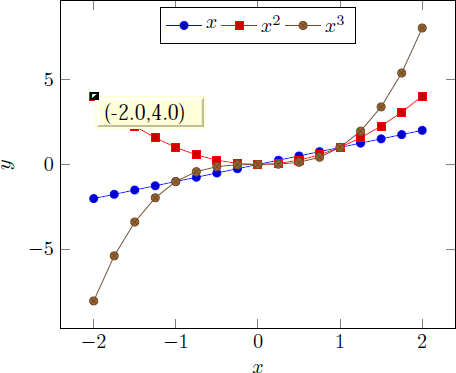
\includegraphics[height=6cm]{figures/pgfplotsclickable-fig1.png}
    \rlap{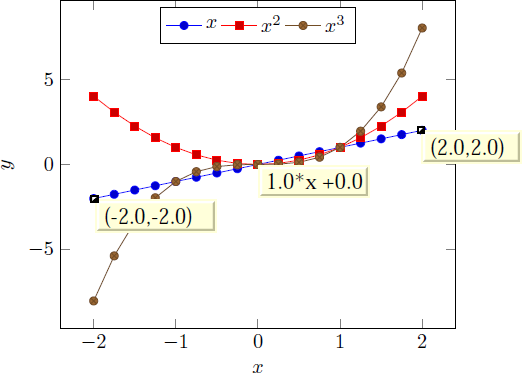
\includegraphics[height=6cm]{figures/pgfplotsclickable-fig2.png}}\hfill

\nobreak These screenshots show the result of clicking into the axis range
(left column) and of dragging from one point to another (right column). The
second case shows the result of Drag-and-Drop: it displays start and end points
and the equation for the line segment between between the first point of the
drag and drop and the second point where the mouse has been released. The line
segment is
%
    \[ l(x; x_0,y_0,x_1,y_1) = m \cdot x + n \]
%
where $m = (y_1-y_0) / (x_1-x_0)$ is the slope and $n$ the offset chosen such
that $l(x_0;\dotsc) = y_0$. For logarithmic plots, logarithms will be applied
before computing slopes.

    \noindent
    \hbox to \linewidth{%
    \hspace{-0.5cm}%
    \begin{tikzpicture}
        \node at (8cm,0cm)    {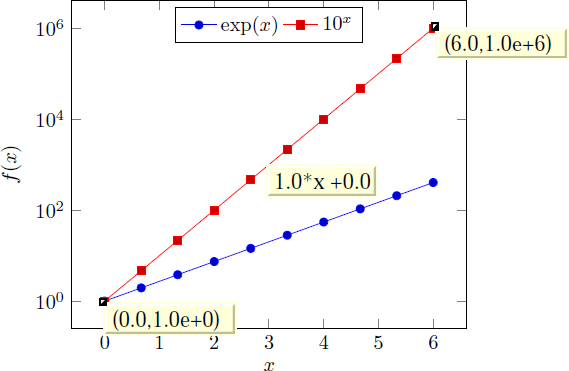
\includegraphics[height=6cm]{figures/pgfplotsclickable-fig4.png}};
        \node at (0cm,0cm)    {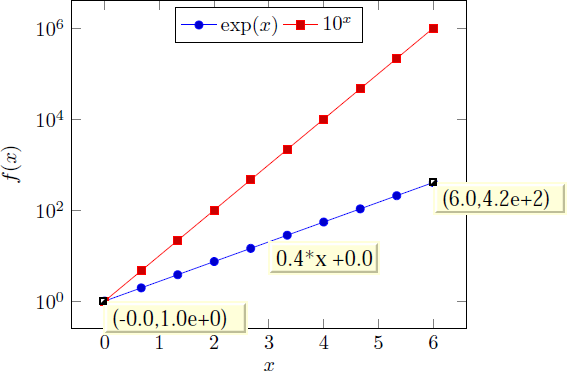
\includegraphics[height=6cm]{figures/pgfplotsclickable-fig3.png}};
    \end{tikzpicture}\hss}%

\nobreak These screen shots show the result of drag- and drop for
\emph{logarithmic} axes: the end points show, again, the coordinates (without
logs) and the form field in the middle shows the slope and offset of the linear
equation in log coordinates.

The log basis for any logarithmic axes is usually~$10$, but it respects the
current setting of |log basis x| and |log basis y|. The applied log will always
use the same logarithm which is also used for the axis descriptions (this is
not necessarily the same as used by \PGFPlotstable!).

This document has been produced with the |clickable| library, so it is possible
to load it into Acrobat Reader and simply click into a plot.

    \expandafter\ifx\csname pgfplotsclickabledisabled\endcsname\relax
    \else
    \paragraph{Attention:}
    For this document, the |clickable| library has been deactivated. You may
    find a different version on \url{http://sourceforge.net/projects/pgfplots}.
    \fi

\begin{pgfplotskey}{clickable coords=\marg{displayed text}}
    Activates a ``snap to nearest'' feature when clicking onto plot
    coordinates. The \meta{displayed text} is the coordinate's $x$ and $y$
    value by default (i.e.\@ you write just |clickable coords| without an equal
    sign).
    %
\begin{codeexample}[]
\begin{tikzpicture}
\begin{loglogaxis}[
    clickable coords={
        Level \thisrow{level} (q=\thisrow{q})
    },
]
    \addplot table [x=dof,y=error] {
        level  dof      error           q
        1      4        2.50000000e-01  48
        2      16       6.25000000e-02  25
        3      64       1.56250000e-02  41
        4      256      3.90625000e-03  8
        5      1024     9.76562500e-04  22
        6      4096     2.44140625e-04  46
        7      16384    6.10351562e-05  40
        8      65536    1.52587891e-05  3
        9      262144   3.81469727e-06  1
        10     1048576  9.53674316e-07  9
    };
\end{loglogaxis}
\end{tikzpicture}
\end{codeexample}
    %
    \noindent Now, clicking onto a data point yields `Level 7 (q=40)' whereas
    clicking besides a data point results in the click coordinates as before,

        \noindent\hbox to \linewidth{\hfill
        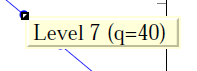
\includegraphics[scale=0.4]{figures/pgfplotsclickable-log-snap0}\hfill
        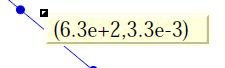
\includegraphics[scale=0.4]{figures/pgfplotsclickable-log-snap2}\hfill
        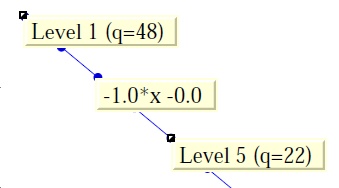
\includegraphics[scale=0.4]{figures/pgfplotsclickable-log-snap1}.\hfill
        }%

    Note that logarithmic slopes work as before.

    If you want the $(x,y)$ values to be displayed, use the special placeholder
    string `|(xy)|' inside of \meta{displayed text}. As an example, we consider
    again the |scatter/classes| example of
    page~\pageref{pgfplots:scatterclasses}:
    %
\begin{codeexample}[]
\begin{tikzpicture}
\begin{axis}[
    clickable coords={(xy): \thisrow{label}},
    scatter/classes={
        a={mark=square*,blue},
        b={mark=triangle*,red},
        c={mark=o,draw=black}   % <-- don't add comma
    }
]
    \addplot [
        only marks,
        scatter,
        scatter src=explicit symbolic
    ] table [meta=label] {
        x     y      label
        0.1   0.15   a
        0.45  0.27   c
        0.02  0.17   a
        0.06  0.1    a
        0.9   0.5    b
        0.5   0.3    c
        0.85  0.52   b
        0.12  0.05   a
        0.73  0.45   b
        0.53  0.25   c
        0.76  0.5    b
        0.55  0.32   c
    };
\end{axis}
\end{tikzpicture}
\end{codeexample}
    %
    \noindent Here, we find popups like

        \noindent\hbox to \linewidth{\hfill
        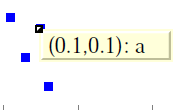
\includegraphics[scale=0.4]{figures/pgfplotsclickable-scatter1.png}\hfill
        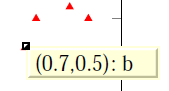
\includegraphics[scale=0.4]{figures/pgfplotsclickable-scatter2.png}\hfill
        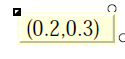
\includegraphics[scale=0.4]{figures/pgfplotsclickable-scatter0.png}.\hfill
        }%

    The \meta{displayed text} is a richtext string displayed with
    \emph{JavaScript}. For most purposes, it is used like an unformatted C
    string: it contains characters, perhaps line breaks with `|\n|' or
    tabulators with `|\t|', but it should not contain \TeX{} formatting
    instructions, especially no math mode (the `|(xy)|' replacement text is
    formatted with |sprintf|, see below). Consider |clickable coords code| in
    case you'd like to preprocess data before displaying it. If you experience
    problems with special characters, try prepending a backslash to them. If
    that doesn't work either, try to prefix the word with `|\\|' and/or with
    `|\string|'. Consider using |clickable coords size| if you intend to work
    with multiline fields and the size allocation needs improvements.

    In fact, \meta{displayed text} can even contain richtext (=XHTML)
    formatting instructions like `|<br/>|' (note the final slash) or
    `|<span style="color:\#7E0000;">text</span>|' (note the backslash before
    `|#|') which changes the color for |text|. The |<span style="">| arguments
    are CSS fields, consider an HTML reference for a list of CSS attributes.

    It is possible to use |clickable coords| together with three dimensional
    axes. Note that dynamic (clickable) features of a three dimensional axis
    without |clickable coords| will be disabled (they appear to be useless).
    Furthermore, three dimensional axes do not support slope calculations; only
    the ``snap to nearest'' feature is available.

    Consider using |annot/snap dist=6| to increase the ``snap to nearest''
    distance.

    The |clickable coords| can be specified for all plots in an axis (as in the
    examples above), but also once for every single |\addplot| commands for
    which the ``snap to nearest'' feature is desired (with different
    \meta{displayed text}).

    If multiple |clickable coords| are on the same position, each click chooses
    the next one (in the order of appearance).
\end{pgfplotskey}

\begin{pgfplotskey}{clickable coords code=\marg{%
    \TeX{} code which defines {\normalfont\ttfamily\textbackslash pgfplotsretval}}%
}
    A variant of |clickable coords| which allows to prepare the displayed
    information before it is handed over to JavaScript.

    The value should be \TeX{} code which defines |\pgfplotsretval| somehow.
    The result is used as simple, unformatted string which is associated to
    coordinates.

    Consider using

    \hspace{2em}|\pgfmathprintnumberto[verbatim]|\marg{number}|\macroname|

    \hspace{2em}|\edef\pgfplotsretval{Number=\macroname}|

    to provide number printing. The |\pgfmathprintnumberto[verbatim]| doesn't
    use math mode to format a number,\footnote{See the \PGFPlotstable{} manual
    for details about number printing.} and it writes its result into
    |\macroname|. The name `|\macroname|' is arbitrary, use anything like
    `|\eps|' or `|\info|'. The |\edef| means ``expanded definition'' and has
    the effect of expanding all macros to determine the value, in our case
    ``Number = \meta{the value}''. The following example uses it twice to
    pretty-print the data:
    %
\begin{codeexample}[]
\begin{tikzpicture}
\begin{loglogaxis}[clickable coords code={
    \pgfmathprintnumberto[verbatim,precision=1]
        {\thisrow{error}}
        \error
    \pgfmathprintnumberto[verbatim,frac]
        {\thisrow{frac}}
        \fraccomp
    \edef\pgfplotsretval{error \error, R=\fraccomp}
}]
    \addplot table [x=dof,y=error] {
        level  dof     error           frac
        1      4       2.50000000e-01  0.5
        2      16      6.25000000e-02  0.75
        3      64      1.56250000e-02  0.1
        4      256     3.90625000e-03  0.2
        5      1024    9.76562500e-04  0.5
        6      4096    2.44140625e-04  0.8
        7      16384   6.10351562e-05  0.125
        8      65536   1.52587891e-05  0.725
        9      262144  3.81469727e-06  0.625
        10     1048576 9.53674316e-07  1
    };
\end{loglogaxis}
\end{tikzpicture}
\end{codeexample}
    %
    \noindent resulting in

        \noindent\hbox to \linewidth{\hfill
        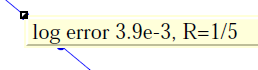
\includegraphics[scale=0.4]{figures/pgfplotsclickable-logcode-snap0.png}\hfill
        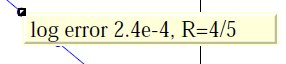
\includegraphics[scale=0.4]{figures/pgfplotsclickable-logcode-snap1.png}.\hfill
        }%

    The \meta{\TeX{} code} is evaluated inside of a local scope, all locally
    declared variables are freed afterwards (that's why you can use any names
    you want).
\end{pgfplotskey}

\begin{pgfplotskey}{%
    clickable coords size=\texttt{auto} or \marg{max chars} or
    \marg{max chars x,max chars y} (initially auto)%
}
    This is actually just another name for |annot/popup size snap|, see its
    documentation below.
\end{pgfplotskey}


\subsection{Requirements for the Library}

\begin{itemize}
    \item The library relies on the \LaTeX{} packages |insdljs| (``Insert
        document level JavaScript'') and |eforms| which are both part of the
        freely available |AcroTeX| education
        bundle~\cite{acrotex}.\footnote{These packages rely on \LaTeX{}, so
        the library is only available for \LaTeX{}, not for plain \TeX{} or
        Con\TeX{}t.} The |insdljs| package creates a temporary file with
        extension |.djs|.
    \item At the time of this writing, only Adobe Acrobat Reader interprets
        JavaScript and Forms properly. The library doesn't have any effect if
        the resulting document is used in other viewers (as far as I know).
\end{itemize}
%
Note that although this library has been written for \PGFPlots{}, it can be
used independently of a \PGFPlots{} environment.


\paragraph{Compatibility issues:}

There a several restrictions when using this library. Most of them will vanish
in future versions -- but up to now, I can't do magic.
%
\begin{itemize}
    \item The library does not yet support rotated axes. Use
        |clickable=false| for those axes.
    \item The library works only with |pdflatex|; |dvips| or |dvipdfm| are not
        supported.\footnote{In fact, they should be. I don't really know why
        they don't. Any hint is welcome.}
    \item Up to now, it is \emph{not} possible to use this library together
        with the |external| library and other image externalization methods of
        Chapter~\ref{cha:pgfplots:importexport}.

        To be more precise, you can (with two extra preamble lines, see below)
        get correctly annotated, exported \pdf{} documents, but the
        |\includegraphics| command does not import the dynamic features.

        In case you decide to use this workaround, you need to insert
        %
\begin{codeexample}[code only]
% \maxdeadcycles=10000 % in case you get the error `Output loop---<N> consecutive dead cycles.'
\usepackage[pdftex]{eforms}
\end{codeexample}
        %
        \noindent \emph{before} loading \pgfname{}, \Tikz{} or \PGFPlots{}. The
        |\maxdeadcycles| appears to be necessary for large documents, try it
        out.

        As long as you are working on a draft version of your document, you
        might want to use
        %
\begin{codeexample}[code only]
\pgfkeys{/pgf/images/include external/.code={\href{file:#1}{\pgfimage{#1}}}}
\end{codeexample}
        %
        in your preamble. This will generate hyperlinks around the graphics
        files which link to the exported figures. Clicking on the hyperlinks
        opens the exported figure which, in turn, has been generated with the
        |clickable| library and allows dynamic features.\footnote{This
        special treatment needs the external files in the same base directory
        as the main document, so this approach is most certainly \emph{not}
        suitable for a final document.}
    \item The library automatically calls |\begin{Form}| at
        |\begin{document}| and |\end{Form}| at the end of the document. This
        environment of |hyperref| is necessary for dynamic user interaction
        and should be kept in mind if the document contains other form
        elements.
\end{itemize}

\paragraph{Acknowledgements:}

\begin{itemize}
    \item I have used a JavaScript |sprintf| implementation of Kevin van
        Zonneveld~\cite{phptojs} (the JavaScript API has only a limited set
        of conversions).
\end{itemize}


\subsection{Customization}

It is possible to customize the library with several options.

\begin{pgfplotskey}{clickable=\mchoice{true,false} (initially true)}
    Allows to disable the library for single plots.
\end{pgfplotskey}

\begin{pgfplotskey}{annot/js fillColor=\marg{JavaScript color} (initially ["RGB",1,1,.855])}
    Sets the background (fill) color of the short popup annotations.

    Possible choices are |transparent|, gray, RGB or CMYK color specified as
    four element arrays of the form
    |["RGB", |\meta{red}|,|\meta{green}|,|\meta{blue}|]|. Each color component
    is between $0$ and $1$.

    Again: this option is for JavaScript. It is \emph{not} possible to use
    colors as in \pgfname{}.
\end{pgfplotskey}

\begin{pgfplotskeylist}{%
    annot/point format=\marg{sprintf-format} (initially {(\%.1f,\%.1f)}),
    annot/point format 3d=\marg{sprintf-format} (initially {(\%.1f,\%.1f,\%.1f)})%
}
    Allows to provide an |sprintf| format string which is used to fill the
    annotations with text. The first argument to |sprintf| is the
    $x$-coordinate and the second argument is the $y$-coordinate.

    The |point format 3d| variant is used for any three-dimensional axis
    whereas the |point format| is used (only) for two-dimensional ones.

    The |every semilogx axis|, |every semilogy axis| and |every loglog axis|
    styles have been updated to
    %
\begin{codeexample}[code only]
\pgfplotsset{
    every semilogy axis/.append style={/pgfplots/annot/point format={(\%.1f,\%.1e)}},
    every semilogx axis/.append style={/pgfplots/annot/point format={(\%.1e,\%.1f)}},
    every loglog axis/.append style={/pgfplots/annot/point format={(\%.1e,\%.1e)}},
}
\end{codeexample}
    %
    \noindent such
    %\todosp{is there a special reason, why the last two entries are not in blue? (on previous page they are blue ...}
    % ... a bug in the highlighting code, I suppose. Fixing it is quite involved and I keep it for now
    that every logarithmic coordinate is displayed in scientific
    format.
\end{pgfplotskeylist}

\begin{pgfplotskey}{annot/slope format=\marg{sprintf-format} (initially \%.1f*x \%+.1f)}
    Allows to provide an |sprintf| format string which is used to fill the
    slope annotation with text. The first argument is the slope and the second
    the line offset.
\end{pgfplotskey}

\begin{pgfplotskey}{annot/printable=\mchoice{true,false} (initially false)}
    Allows to configure whether the small annotations will be printed.
    Otherwise, they are only available on screen.
\end{pgfplotskey}

\begin{pgfplotskey}{annot/font=\marg{JavaScript font name} (initially font.Times)}
    Allows to choose a JavaScript font for the annotations. Possible choices
    are limited to what JavaScript accepts (which is \emph{not} the same as
    \LaTeX{}). The default fonts and its names are shown below.

    \begin{center}
        \begin{tabular}{ll}
                \toprule
            Font Name             & Name in JavaScript \\
                \midrule
            Times-Roman           & font.Times         \\
            Times-Bold            & font.TimesB        \\
            Times-Italic          & font.TimesI        \\
            Times-BoldItalic      & font.TimesBI       \\
            Helvetica             & font.Helv          \\
            Helvetica-Bold        & font.HelvB         \\
            Helvetica-Oblique     & font.HelvI         \\
            Helvetica-BoldOblique & font.HelvBI        \\
            Courier               & font.Cour          \\
            Courier-Bold          & font.CourB         \\
            Courier-Oblique       & font.CourI         \\
            Courier-BoldOblique   & font.CourBI        \\
            Symbol                & font.Symbol        \\
            ZapfDingbats          & font.ZapfD         \\
                \bottomrule
        \end{tabular}
    \end{center}
\end{pgfplotskey}

\begin{pgfplotskey}{annot/textSize=\marg{Size in Point} (initially 11)}
    Sets the text size of annotations in points.
\end{pgfplotskey}

\begin{pgfplotskeylist}{%
    annot/popup size generic=\texttt{auto} or \marg{x} or \marg{x,y} (initially auto),
    annot/popup size snap=\texttt{auto} or \marg{x} or \marg{x,y} (initially auto),
    annot/popup size=\marg{value}%
}
    The first key defines the size of popups if you just click into an axis.
    The second key defines the size of popups for the ``snap to nearest''
    feature (i.e.\@ those prepared by |clickable coords|). The third key sets
    both to the same \meta{value}.

    The argument can be |auto| in which case \PGFPlots{} tries to be smart and
    counts characters. This may fail for multiline texts. The choice \meta{x}
    provides the \emph{horizontal} size only, in units of |annot/textSize|.
    Thus, |annot/popup size generic=6| makes the popup $6\cdot 11$ points wide.
    In this case, only one line will be allocated. Finally, \meta{x,y} allows
    to provide horizontal and vertical size, both in units of |annot/textSize|.

    See also |clickable coords size| which is an alias for
    |annot/popup size snap|.
\end{pgfplotskeylist}

\begin{pgfplotskey}{annot/snap dist=\marg{Size in Point} (initially 4)}
    Defines the size within two mouse clicks are considered to be equivalent,
    measured in points (Euclidean distance).
\end{pgfplotskey}

\begin{pgfplotskey}{annot/richtext=\mchoice{true,false} (initially true)}
    Enables or disables richtext formatting in |clickable coords| arguments.
    Richtext is kind of XHTML and allows CSS styles like colors, font changes
    and other CSS attributes, see the documentation for |clickable coords| for
    details.

    The case |annot/richtext=false| is probably more robust.
\end{pgfplotskey}


\subsection{Using the Clickable Library in Other Contexts}

This library provides essentially one command, |\pgfplotsclickablecreate| which
creates a clickable area of predefined size, combined with JavaScript
interaction code. It can be used independently of \PGFPlots{}.

\begin{command}{\pgfplotsclickablecreate\oarg{required key-value-options}}
    Creates an area which is clickable. A click produces a popup which contains
    information about the point under the cursor.

    The complete (!) context needs to be provided using key--value pairs, either
    set before calling this method of inside of
    \oarg{required key-value-options}.

    This command actually creates an AcroForm which invokes JavaScript whenever
    it is clicked. A JavaScript Object is created which represents the context
    (axis limits and options). This JavaScript object is available at runtime.

    This method is public and it is \emph{not} restricted to \PGFPlots{}. The
    \PGFPlots{} hook simply initializes the required key--value pairs.

    This method does not draw anything. It initializes only a clickable area
    and JavaScript code.

    The required key--value pairs are documented below.

    \paragraph{Attention:}

    Complete key--value validation is \emph{not} performed here. It can happen
    that invalid options will produce JavaScript bugs when opened with Acrobat
    Reader. Use the JavaScript console to find them.
\end{command}

\noindent All options described in the following are only interesting for users
who intend to use this library without \PGFPlots{}.

\begin{pgfplotskey}{annot/width=\marg{dimension} (initially -)}
    This required key communicates the area's width to
    |\pgfplotsclickablecreate|. It must be a \TeX{} dimension like |5cm|.
\end{pgfplotskey}

\begin{pgfplotskey}{annot/height=\marg{dimension} (initially -)}
    This required key communicates the area's height to
    |\pgfplotsclickablecreate|. It must be a \TeX{} dimension like |5cm|.
\end{pgfplotskey}

\begin{pgfplotskey}{annot/jsname=\marg{string} (initially -)}
    This required key communicates a unique identifier to
    |\pgfplotsclickablecreate|. This identifier is used to identify the object
    in JavaScript, so there can't be more than one of them. If it is empty, a
    default identifier will be generated.
\end{pgfplotskey}

\begin{pgfplotskeylist}{%
    annot/xmin=\marg{number},
    annot/xmax=\marg{number},
    annot/ymin=\marg{number},
    annot/ymax=\marg{number} (initially empty)%
}
    These required keys communicate the axis limits to
    |\pgfplotsclickablecreate|. They should be set to numbers which can be
    assigned to a JavaScript floating point number (standard IEEE double
    precision).
\end{pgfplotskeylist}

\begin{pgfplotskey}{annot/collected plots=\marg{nested arrays} (initially empty)}
    The low level interface to implement a ``snap to nearest'' feature. The
    value is an array of plots, where each plot is again an array of
    coordinates and each coordinate is an array of three elements, $x$, $y$ and
    text. Please consult the code comments for details and examples.
\end{pgfplotskey}
\endgroup


\begingroup
\tikzset{external/figure name/.add={}{brewer_}}%
    \tikzset{
%        font=\scriptsize,
        matrix style/.style={
            font=\tiny,
            every matrix/.append style={
                matrix anchor=north,
                inner ysep=0pt,
%                fill=red!10,
                ampersand replacement=\&,
                matrix of nodes,
                nodes={
                    anchor=south,
                    minimum size=2mm,
                },
                row 1/.style={
                    inner sep=0pt,
                },
                column 1/.style={
                    inner ysep=0pt,
                    anchor=base east,
                },
                row 2 column 1/.style={
                    every node/.append style={
                        font=\bfseries\scriptsize,
%                        font=\bfseries\tiny,
                        draw,
                    },
                },
                row sep=0pt,
                column sep=0pt,
            },
        },
    }


% =============================================================================
%\def\MATRIXseq#1{%
\NewDocumentCommand{\MATRIXseq}{sm}{{%
\tikzset{/tikz/external/export=true}%
\newcommand*\scheme{#2}%
\pgfmanualpdflabel{colormap/\scheme-3}{}%
\pgfmanualpdflabel{colormap/\scheme-4}{}%
\pgfmanualpdflabel{colormap/\scheme-5}{}%
\pgfmanualpdflabel{colormap/\scheme-6}{}%
\pgfmanualpdflabel{colormap/\scheme-7}{}%
\pgfmanualpdflabel{colormap/\scheme-8}{}%
\pgfmanualpdflabel{colormap/\scheme-9}{}%
\pgfmanualpdflabel{colormap/\scheme}{}%
\foreach \x in {A,...,M} {\pgfmanualpdflabel{\scheme-\x}{}}%
\tikzsetnextfilename{brewer-seq-#2}%
\begin{tikzpicture}[
    matrix style,
]
    % instantiate all colormaps for \scheme:
    \pgfplotsset{
        colormap/\scheme-3,
        colormap/\scheme-4,
        colormap/\scheme-5,
        colormap/\scheme-6,
        colormap/\scheme-7,
        colormap/\scheme-8,
        colormap/\scheme-9,
        colormap/\scheme,
    }%
    %
    % directly access the correct color:
    % #1 is one of A,B,...,M
    \def\C##1{\node [fill=\scheme-##1] {};}%
    % in case the color should be white, also draw a black frame
    \def\D##1{\node [draw=black,fill=\scheme-##1] {};}%
    %
    % indirectly access the correct color
    % #1 is an index into the colormap, 0,1,...,13
    % #2 is the number of colors in the colormap (qualifies which colormap to use)
    % This is redundant, but it allows us to verify that the colormaps
    % work as intended without typos:
    \newcommand*\CC[2]{\node [/pgfplots/index of colormap=##1 of \scheme-##2, fill] {};}%
    % in case the color should be white, also draw a black frame
    \newcommand*\DD[2]{\node [/pgfplots/index of colormap=##1 of \scheme-##2, fill, draw=black] {};}%
    %
    % define a colorbar that has the same size as a row of colors in the matrix
    \newcommand*\CM{%
        \node[inner sep=0pt,xshift=-3.5pt,overlay,anchor=south west]{%
\IfBooleanTF{#1}{%
            \pgfmathparse{14*2mm + 16*\pgflinewidth + 1.0pt}%
}{%
            \pgfmathparse{14*2mm + 15*\pgflinewidth + 1.1pt}%
}
            \let\width=\pgfmathresult
            \pgfplotscolormaptoshadingspec{\scheme}{\width pt}\result
            \def\tempb{\pgfdeclarehorizontalshading{tempshading}{2mm}}%
            \expandafter\tempb\expandafter{\result}%
            \pgfuseshading{tempshading}%
        };
    }%
    \matrix {
\IfBooleanTF{#1}{%
                \& A         \& B         \& C         \& D         \& E         \& F         \& G         \& H         \& I         \& J         \& K         \& L         \& M         \\
        \scheme \& \D{A}     \& \C{B}     \& \C{C}     \& \C{D}     \& \C{E}     \& \C{F}     \& \C{G}     \& \C{H}     \& \C{I}     \& \C{J}     \& \C{K}     \& \C{L}     \& \C{M}     \\
        3       \&           \&           \& \CC{0}{3} \&           \&           \& \CC{1}{3} \&           \&           \& \CC{2}{3} \&           \&           \&           \&           \\
        4       \&           \& \CC{0}{4} \&           \&           \& \CC{1}{4} \&           \& \CC{2}{4} \&           \&           \& \CC{3}{4} \&           \&           \&           \\
        5       \&           \& \CC{0}{5} \&           \&           \& \CC{1}{5} \&           \& \CC{2}{5} \&           \& \CC{3}{5} \&           \& \CC{4}{5} \&           \&           \\
        6       \&           \& \CC{0}{6} \&           \& \CC{1}{6} \&           \& \CC{2}{6} \& \CC{3}{6} \&           \& \CC{4}{6} \&           \& \CC{5}{6} \&           \&           \\
        7       \&           \& \CC{0}{7} \&           \& \CC{1}{7} \&           \& \CC{2}{7} \& \CC{3}{7} \& \CC{4}{7} \&           \& \CC{5}{7} \&           \& \CC{6}{7} \&           \\
        8       \& \DD{0}{8} \&           \& \CC{1}{8} \& \CC{2}{8} \&           \& \CC{3}{8} \& \CC{4}{8} \& \CC{5}{8} \&           \& \CC{6}{8} \&           \& \CC{7}{8} \&           \\
        9       \& \DD{0}{9} \&           \& \CC{1}{9} \& \CC{2}{9} \&           \& \CC{3}{9} \& \CC{4}{9} \& \CC{5}{9} \&           \& \CC{6}{9} \& \CC{7}{9} \&           \& \CC{8}{9} \\
        CM      \& \CM       \&           \&           \&           \&           \&           \&           \&           \&           \&           \&           \&           \&           \\
%                \& A         \& B         \& C         \& D         \& E         \& F         \& G         \& H         \& I         \& J         \& K         \& L         \& M         \\
%                \& \D{A}     \& \C{B}     \& \C{C}     \& \C{D}     \& \C{E}     \& \C{F}     \& \C{G}     \& \C{H}     \& \C{I}     \& \C{J}     \& \C{K}     \& \C{L}     \& \C{M}     \\
%                \&           \&           \& \CC{0}{3} \&           \&           \& \CC{1}{3} \&           \&           \& \CC{2}{3} \&           \&           \&           \&           \\
%                \&           \& \CC{0}{4} \&           \&           \& \CC{1}{4} \&           \& \CC{2}{4} \&           \&           \& \CC{3}{4} \&           \&           \&           \\
%                \&           \& \CC{0}{5} \&           \&           \& \CC{1}{5} \&           \& \CC{2}{5} \&           \& \CC{3}{5} \&           \& \CC{4}{5} \&           \&           \\
%                \&           \& \CC{0}{6} \&           \& \CC{1}{6} \&           \& \CC{2}{6} \& \CC{3}{6} \&           \& \CC{4}{6} \&           \& \CC{5}{6} \&           \&           \\
%                \&           \& \CC{0}{7} \&           \& \CC{1}{7} \&           \& \CC{2}{7} \& \CC{3}{7} \& \CC{4}{7} \&           \& \CC{5}{7} \&           \& \CC{6}{7} \&           \\
%                \& \DD{0}{8} \&           \& \CC{1}{8} \& \CC{2}{8} \&           \& \CC{3}{8} \& \CC{4}{8} \& \CC{5}{8} \&           \& \CC{6}{8} \&           \& \CC{7}{8} \&           \\
%                \& \DD{0}{9} \&           \& \CC{1}{9} \& \CC{2}{9} \&           \& \CC{3}{9} \& \CC{4}{9} \& \CC{5}{9} \&           \& \CC{6}{9} \& \CC{7}{9} \&           \& \CC{8}{9} \\
}{%
                \& A         \& B         \& C         \& D         \& E         \& F         \& G         \& H         \& I         \& J         \& K         \& L         \& M         \\
        \scheme \& \C{A}     \& \C{B}     \& \C{C}     \& \C{D}     \& \C{E}     \& \C{F}     \& \C{G}     \& \C{H}     \& \C{I}     \& \C{J}     \& \C{K}     \& \C{L}     \& \C{M}     \\
        3       \&           \&           \& \CC{0}{3} \&           \&           \& \CC{1}{3} \&           \&           \& \CC{2}{3} \&           \&           \&           \&           \\
        4       \&           \& \CC{0}{4} \&           \&           \& \CC{1}{4} \&           \& \CC{2}{4} \&           \&           \& \CC{3}{4} \&           \&           \&           \\
        5       \&           \& \CC{0}{5} \&           \&           \& \CC{1}{5} \&           \& \CC{2}{5} \&           \& \CC{3}{5} \&           \& \CC{4}{5} \&           \&           \\
        6       \&           \& \CC{0}{6} \&           \& \CC{1}{6} \&           \& \CC{2}{6} \& \CC{3}{6} \&           \& \CC{4}{6} \&           \& \CC{5}{6} \&           \&           \\
        7       \&           \& \CC{0}{7} \&           \& \CC{1}{7} \&           \& \CC{2}{7} \& \CC{3}{7} \& \CC{4}{7} \&           \& \CC{5}{7} \&           \& \CC{6}{7} \&           \\
        8       \& \CC{0}{8} \&           \& \CC{1}{8} \& \CC{2}{8} \&           \& \CC{3}{8} \& \CC{4}{8} \& \CC{5}{8} \&           \& \CC{6}{8} \&           \& \CC{7}{8} \&           \\
        9       \& \CC{0}{9} \&           \& \CC{1}{9} \& \CC{2}{9} \&           \& \CC{3}{9} \& \CC{4}{9} \& \CC{5}{9} \&           \& \CC{6}{9} \& \CC{7}{9} \&           \& \CC{8}{9} \\
        CM      \& \CM       \&           \&           \&           \&           \&           \&           \&           \&           \&           \&           \&           \&           \\
%                \& A         \& B         \& C         \& D         \& E         \& F         \& G         \& H         \& I         \& J         \& K         \& L         \& M         \\
%                \& \C{A}     \& \C{B}     \& \C{C}     \& \C{D}     \& \C{E}     \& \C{F}     \& \C{G}     \& \C{H}     \& \C{I}     \& \C{J}     \& \C{K}     \& \C{L}     \& \C{M}     \\
%                \&           \&           \& \CC{0}{3} \&           \&           \& \CC{1}{3} \&           \&           \& \CC{2}{3} \&           \&           \&           \&           \\
%                \&           \& \CC{0}{4} \&           \&           \& \CC{1}{4} \&           \& \CC{2}{4} \&           \&           \& \CC{3}{4} \&           \&           \&           \\
%                \&           \& \CC{0}{5} \&           \&           \& \CC{1}{5} \&           \& \CC{2}{5} \&           \& \CC{3}{5} \&           \& \CC{4}{5} \&           \&           \\
%                \&           \& \CC{0}{6} \&           \& \CC{1}{6} \&           \& \CC{2}{6} \& \CC{3}{6} \&           \& \CC{4}{6} \&           \& \CC{5}{6} \&           \&           \\
%                \&           \& \CC{0}{7} \&           \& \CC{1}{7} \&           \& \CC{2}{7} \& \CC{3}{7} \& \CC{4}{7} \&           \& \CC{5}{7} \&           \& \CC{6}{7} \&           \\
%                \& \CC{0}{8} \&           \& \CC{1}{8} \& \CC{2}{8} \&           \& \CC{3}{8} \& \CC{4}{8} \& \CC{5}{8} \&           \& \CC{6}{8} \&           \& \CC{7}{8} \&           \\
%                \& \CC{0}{9} \&           \& \CC{1}{9} \& \CC{2}{9} \&           \& \CC{3}{9} \& \CC{4}{9} \& \CC{5}{9} \&           \& \CC{6}{9} \& \CC{7}{9} \&           \& \CC{8}{9} \\
}
    };
\end{tikzpicture}%
}}

\NewDocumentCommand{\MATRIXdiv}{sm}{{%
\newcommand*\scheme{#2}%
\tikzset{/tikz/external/export=true}%
\pgfmanualpdflabel{colormap/\scheme-3}{}%
\pgfmanualpdflabel{colormap/\scheme-4}{}%
\pgfmanualpdflabel{colormap/\scheme-5}{}%
\pgfmanualpdflabel{colormap/\scheme-6}{}%
\pgfmanualpdflabel{colormap/\scheme-7}{}%
\pgfmanualpdflabel{colormap/\scheme-8}{}%
\pgfmanualpdflabel{colormap/\scheme-9}{}%
\pgfmanualpdflabel{colormap/\scheme-10}{}%
\pgfmanualpdflabel{colormap/\scheme-11}{}%
\pgfmanualpdflabel{colormap/\scheme}{}%
\foreach \x in {A,...,O} {\pgfmanualpdflabel{\scheme-\x}{}}%
\tikzsetnextfilename{brewer-div-#2}%
\begin{tikzpicture}[
    matrix style,
]
    % instantiate all colormaps for \scheme:
    \pgfplotsset{
        colormap/\scheme-3,
        colormap/\scheme-4,
        colormap/\scheme-5,
        colormap/\scheme-6,
        colormap/\scheme-7,
        colormap/\scheme-8,
        colormap/\scheme-9,
        colormap/\scheme-10,
        colormap/\scheme-11,
        colormap/\scheme,
    }%
    %
    % directly access the correct color:
    % #1 is one of A,B,...,M
    \def\C##1{\node [fill=\scheme-##1] {};}%
    % in case the color should be white, also draw a black frame
    \def\D##1{\node [draw=black,fill=\scheme-##1] {};}%
    %
    % indirectly access the correct color
    % #1 is an index into the colormap, 0,1,...,13
    % #2 is the number of colors in the colormap (qualifies which colormap to use)
    % This is redundant, but it allows us to verify that the colormaps
    % work as intended without typos:
    \newcommand*\CC[2]{\node [/pgfplots/index of colormap=##1 of \scheme-##2, fill] {};}%
    % in case the color should be white, also draw a black frame
    \newcommand*\DD[2]{\node [/pgfplots/index of colormap=##1 of \scheme-##2, fill, draw=black] {};}%
    %
    % define a colorbar that has the same size as a row of colors in the matrix
    \newcommand*\CM{%
        \node[inner sep=0pt,xshift=-3.5pt,overlay,anchor=south west]{%
\IfBooleanTF{#1}{%
            \pgfmathparse{16*2mm + 18*\pgflinewidth + 2.3pt}%
}{%
            \pgfmathparse{16*2mm + 17*\pgflinewidth + 2.3pt}%
}%
            \let\width=\pgfmathresult
            \pgfplotscolormaptoshadingspec{\scheme}{\width pt}\result
            \def\tempb{\pgfdeclarehorizontalshading{tempshading}{2mm}}%
            \expandafter\tempb\expandafter{\result}%
            \pgfuseshading{tempshading}%
        };
    }%
    \matrix {
\IfBooleanTF{#1}{%
                \& A          \& B          \& C         \& D          \& E         \& F          \& G          \& H          \& I          \& J          \& K         \& L          \& M         \& N          \& O           \\
        \scheme \& \C{A}      \& \C{B}      \& \C{C}     \& \C{D}      \& \C{E}     \& \C{F}      \& \C{G}      \& \D{H}      \& \C{I}      \& \C{J}      \& \C{K}     \& \C{L}      \& \C{M}     \& \C{N}      \& \C{O}       \\
        3       \&            \&            \&           \&            \& \CC{0}{3} \&            \&            \& \DD{1}{3}  \&            \&            \& \CC{2}{3} \&            \&           \&            \&             \\
        4       \&            \&            \& \CC{0}{4} \&            \&           \& \CC{1}{4}  \&            \&            \&            \& \CC{2}{4}  \&           \&            \& \CC{3}{4} \&            \&             \\
        5       \&            \&            \& \CC{0}{5} \&            \&           \& \CC{1}{5}  \&            \& \DD{2}{5}  \&            \& \CC{3}{5}  \&           \&            \& \CC{4}{5} \&            \&             \\
        6       \&            \& \CC{0}{6}  \&           \&            \& \CC{1}{7} \&            \& \CC{2}{6}  \&            \& \CC{3}{6}  \&            \& \CC{4}{6} \&            \&           \& \CC{5}{6}  \&             \\
        7       \&            \& \CC{0}{7}  \&           \&            \& \CC{1}{7} \&            \& \CC{2}{7}  \& \DD{3}{7}  \& \CC{4}{7}  \&            \& \CC{5}{7} \&            \&           \& \CC{6}{7}  \&             \\
        8       \&            \& \CC{0}{8}  \&           \& \CC{1}{8}  \&           \& \CC{2}{8}  \& \CC{3}{8}  \&            \& \CC{4}{8}  \& \CC{5}{8}  \&           \& \CC{6}{8}  \&           \& \CC{7}{8}  \&             \\
        9       \&            \& \CC{0}{9}  \&           \& \CC{1}{9}  \&           \& \CC{2}{9}  \& \CC{3}{9}  \& \DD{4}{9}  \& \CC{5}{9}  \& \CC{6}{9}  \&           \& \CC{7}{9}  \&           \& \CC{8}{9}  \&             \\
        10      \& \CC{0}{10} \& \CC{1}{10} \&           \& \CC{2}{10} \&           \& \CC{3}{10} \& \CC{4}{10} \&            \& \CC{5}{10} \& \CC{6}{10} \&           \& \CC{7}{10} \&           \& \CC{8}{10} \& \CC{9}{10}  \\
        11      \& \CC{0}{11} \& \CC{1}{11} \&           \& \CC{2}{11} \&           \& \CC{3}{11} \& \CC{4}{11} \& \DD{5}{11} \& \CC{6}{11} \& \CC{7}{11} \&           \& \CC{8}{11} \&           \& \CC{9}{11} \& \CC{10}{11} \\
        CM      \& \CM        \&            \&           \&            \&           \&            \&            \&            \&            \&            \&           \&            \&           \&            \&             \\
}{%
                \& A          \& B          \& C         \& D          \& E         \& F          \& G          \& H          \& I          \& J          \& K         \& L          \& M         \& N          \& O           \\
        \scheme \& \C{A}      \& \C{B}      \& \C{C}     \& \C{D}      \& \C{E}     \& \C{F}      \& \C{G}      \& \C{H}      \& \C{I}      \& \C{J}      \& \C{K}     \& \C{L}      \& \C{M}     \& \C{N}      \& \C{O}       \\
        3       \&            \&            \&           \&            \& \CC{0}{3} \&            \&            \& \CC{1}{3}  \&            \&            \& \CC{2}{3} \&            \&           \&            \&             \\
        4       \&            \&            \& \CC{0}{4} \&            \&           \& \CC{1}{4}  \&            \&            \&            \& \CC{2}{4}  \&           \&            \& \CC{3}{4} \&            \&             \\
        5       \&            \&            \& \CC{0}{5} \&            \&           \& \CC{1}{5}  \&            \& \CC{2}{5}  \&            \& \CC{3}{5}  \&           \&            \& \CC{4}{5} \&            \&             \\
        6       \&            \& \CC{0}{6}  \&           \&            \& \CC{1}{7} \&            \& \CC{2}{6}  \&            \& \CC{3}{6}  \&            \& \CC{4}{6} \&            \&           \& \CC{5}{6}  \&             \\
        7       \&            \& \CC{0}{7}  \&           \&            \& \CC{1}{7} \&            \& \CC{2}{7}  \& \CC{3}{7}  \& \CC{4}{7}  \&            \& \CC{5}{7} \&            \&           \& \CC{6}{7}  \&             \\
        8       \&            \& \CC{0}{8}  \&           \& \CC{1}{8}  \&           \& \CC{2}{8}  \& \CC{3}{8}  \&            \& \CC{4}{8}  \& \CC{5}{8}  \&           \& \CC{6}{8}  \&           \& \CC{7}{8}  \&             \\
        9       \&            \& \CC{0}{9}  \&           \& \CC{1}{9}  \&           \& \CC{2}{9}  \& \CC{3}{9}  \& \CC{4}{9}  \& \CC{5}{9}  \& \CC{6}{9}  \&           \& \CC{7}{9}  \&           \& \CC{8}{9}  \&             \\
        10      \& \CC{0}{10} \& \CC{1}{10} \&           \& \CC{2}{10} \&           \& \CC{3}{10} \& \CC{4}{10} \&            \& \CC{5}{10} \& \CC{6}{10} \&           \& \CC{7}{10} \&           \& \CC{8}{10} \& \CC{9}{10}  \\
        11      \& \CC{0}{11} \& \CC{1}{11} \&           \& \CC{2}{11} \&           \& \CC{3}{11} \& \CC{4}{11} \& \CC{5}{11} \& \CC{6}{11} \& \CC{7}{11} \&           \& \CC{8}{11} \&           \& \CC{9}{11} \& \CC{10}{11} \\
        CM      \& \CM        \&            \&           \&            \&           \&            \&            \&            \&            \&            \&           \&            \&           \&            \&             \\
}
    };
\end{tikzpicture}%
}}

\NewDocumentCommand{\MATRIXqual}{mmO{0}}{{%
\tikzset{/tikz/external/export=true}%
\newcommand*\scheme{#2}%
\pgfmanualpdflabel{colormap/\scheme-3}{}%
\pgfmanualpdflabel{colormap/\scheme-4}{}%
\pgfmanualpdflabel{colormap/\scheme-5}{}%
\pgfmanualpdflabel{colormap/\scheme-6}{}%
\pgfmanualpdflabel{colormap/\scheme-7}{}%
\pgfmanualpdflabel{colormap/\scheme-8}{}%
\ifnum#1>8
\pgfmanualpdflabel{colormap/\scheme-9}{}%
\ifnum#1>9
\pgfmanualpdflabel{colormap/\scheme-10}{}%
\pgfmanualpdflabel{colormap/\scheme-11}{}%
\pgfmanualpdflabel{colormap/\scheme-12}{}%
\fi
\fi
\pgfmanualpdflabel{colormap/\scheme}{}%
\tikzsetnextfilename{brewer-qualit-#2}%
\begin{tikzpicture}[
    baseline,
    matrix style,
]
    \newcommand*\classes{#1}%
    % instantiate all colormaps for \scheme:
    \pgfplotsset{
        colormap/\scheme-3,
        colormap/\scheme-4,
        colormap/\scheme-5,
        colormap/\scheme-6,
        colormap/\scheme-7,
        colormap/\scheme-8,
    }
\foreach \x in {A,...,H} {\pgfmanualpdflabel{\scheme-\x}{}}%
\ifnum\classes>8
\foreach \x in {I} {\pgfmanualpdflabel{\scheme-\x}{}}%
    \pgfplotsset{
        colormap/\scheme-9,
    }
\fi
\ifnum\classes=12
\foreach \x in {J,...,L} {\pgfmanualpdflabel{\scheme-\x}{}}%
    \pgfplotsset{
        colormap/\scheme-10,
        colormap/\scheme-11,
        colormap/\scheme-12,
    }
\fi
    \pgfplotsset{
        colormap/\scheme,
    }%
    %
    \newcommand*\EmptyRows{#3}

    % directly access the correct color:
    % #1 is one of A,B,...,M
    \def\C##1{\node [fill=\scheme-##1] {};}
    %
    % indirectly access the correct color
    % #1 is an index into the colormap, 0,1,...,13
    % #2 is the number of colors in the colormap (qualifies which colormap to use)
    % This is redundant, but it allows us to verify that the colormaps
    % work as intended without typos:
    \newcommand*\CC[2]{\node [/pgfplots/index of colormap=##1 of \scheme-##2, fill] {};}
    %
    % define dummy node to just produce space
    \newcommand*\Dummy{\node {};}
%    % define a colorbar that has the same size as a row of colors in the matrix
%\ifnum\classes=8
%    \newcommand*\CM{%
%        \node[inner sep=0pt,xshift=-3.5pt,overlay,anchor=south west]{%
%                \pgfmathparse{8*2mm + 8pt}%
%            \let\width=\pgfmathresult%
%            \pgfplotscolormaptoshadingspec{\scheme}{\width pt}\result%
%            \def\tempb{\pgfdeclarehorizontalshading{tempshading}{2mm}}%
%            \expandafter\tempb\expandafter{\result}%
%            \pgfuseshading{tempshading}%
%        };
%    }
%\else\ifnum\classes=9
%    \newcommand*\CM{%
%        \node[inner sep=0pt,xshift=-3.5pt,overlay,anchor=south west]{%
%                \pgfmathparse{9*2mm + 10*\pgflinewidth + 2.3pt}%
%            \let\width=\pgfmathresult%
%            \pgfplotscolormaptoshadingspec{\scheme}{\width pt}\result%
%            \def\tempb{\pgfdeclarehorizontalshading{tempshading}{2mm}}%
%            \expandafter\tempb\expandafter{\result}%
%            \pgfuseshading{tempshading}%
%        };
%    }
%\else\ifnum\classes=12
%    \newcommand*\CM{%
%        \node[inner sep=0pt,xshift=-3.5pt,overlay,anchor=south west]{%
%                \pgfmathparse{12*2mm + 13*\pgflinewidth + 2.3pt}%
%            \let\width=\pgfmathresult%
%            \pgfplotscolormaptoshadingspec{\scheme}{\width pt}\result%
%            \def\tempb{\pgfdeclarehorizontalshading{tempshading}{2mm}}%
%            \expandafter\tempb\expandafter{\result}%
%            \pgfuseshading{tempshading}%
%        };
%    }
%\fi\fi\fi
\ifnum\classes=8
    \matrix (m) {
                \& A          \& B          \& C          \& D          \& E          \& F          \& G          \& H          \\
        \scheme \& \C{A}      \& \C{B}      \& \C{C}      \& \C{D}      \& \C{E}      \& \C{F}      \& \C{G}      \& \C{H}      \\
        3       \& \CC{0}{3}  \& \CC{1}{3}  \& \CC{2}{3}  \&            \&            \&            \&            \&            \\
        4       \& \CC{0}{4}  \& \CC{1}{4}  \& \CC{2}{4}  \& \CC{3}{4}  \&            \&            \&            \&            \\
        5       \& \CC{0}{5}  \& \CC{1}{5}  \& \CC{2}{5}  \& \CC{3}{5}  \& \CC{4}{5}  \&            \&            \&            \\
        6       \& \CC{0}{6}  \& \CC{1}{6}  \& \CC{2}{6}  \& \CC{3}{6}  \& \CC{4}{6}  \& \CC{5}{6}  \&            \&            \\
        7       \& \CC{0}{7}  \& \CC{1}{7}  \& \CC{2}{7}  \& \CC{3}{7}  \& \CC{4}{7}  \& \CC{5}{7}  \& \CC{6}{7}  \&            \\
        8       \& \CC{0}{8}  \& \CC{1}{8}  \& \CC{2}{8}  \& \CC{3}{8}  \& \CC{4}{8}  \& \CC{5}{8}  \& \CC{6}{8}  \& \CC{7}{8}  \& \Dummy \& \Dummy \& \Dummy \& \Dummy \\
%%%%%        CM      \& \CM        \&            \&            \&            \&            \&            \&            \&            \\
    };
\else\ifnum\classes=9
    \matrix (m) {
                \& A          \& B          \& C          \& D          \& E          \& F          \& G          \& H          \& I         \\
        \scheme \& \C{A}      \& \C{B}      \& \C{C}      \& \C{D}      \& \C{E}      \& \C{F}      \& \C{G}      \& \C{H}      \& \C{I}     \\
        3       \& \CC{0}{3}  \& \CC{1}{3}  \& \CC{2}{3}  \&            \&            \&            \&            \&            \&           \\
        4       \& \CC{0}{4}  \& \CC{1}{4}  \& \CC{2}{4}  \& \CC{3}{4}  \&            \&            \&            \&            \&           \\
        5       \& \CC{0}{5}  \& \CC{1}{5}  \& \CC{2}{5}  \& \CC{3}{5}  \& \CC{4}{5}  \&            \&            \&            \&           \\
        6       \& \CC{0}{6}  \& \CC{1}{6}  \& \CC{2}{6}  \& \CC{3}{6}  \& \CC{4}{6}  \& \CC{5}{6}  \&            \&            \&           \\
        7       \& \CC{0}{7}  \& \CC{1}{7}  \& \CC{2}{7}  \& \CC{3}{7}  \& \CC{4}{7}  \& \CC{5}{7}  \& \CC{6}{7}  \&            \&           \\
        8       \& \CC{0}{8}  \& \CC{1}{8}  \& \CC{2}{8}  \& \CC{3}{8}  \& \CC{4}{8}  \& \CC{5}{8}  \& \CC{6}{8}  \& \CC{7}{8}  \&           \\
        9       \& \CC{0}{9}  \& \CC{1}{9}  \& \CC{2}{9}  \& \CC{3}{9}  \& \CC{4}{9}  \& \CC{5}{9}  \& \CC{6}{9}  \& \CC{7}{9}  \& \CC{8}{9} \& \Dummy \& \Dummy \& \Dummy \\
%%%%%        CM      \& \CM        \&            \&            \&            \&            \&            \&            \&            \&           \\
    };
\else\ifnum\classes=12
    \matrix (m) {
                \& A          \& B          \& C          \& D          \& E          \& F          \& G          \& H          \& I          \& J          \& K           \& L           \\
        \scheme \& \C{A}      \& \C{B}      \& \C{C}      \& \C{D}      \& \C{E}      \& \C{F}      \& \C{G}      \& \C{H}      \& \C{I}      \& \C{J}      \& \C{K}       \& \C{L}       \\
        3       \& \CC{0}{3}  \& \CC{1}{3}  \& \CC{2}{3}  \&            \&            \&            \&            \&            \&            \&            \&             \&             \\
        4       \& \CC{0}{4}  \& \CC{1}{4}  \& \CC{2}{4}  \& \CC{3}{4}  \&            \&            \&            \&            \&            \&            \&             \&             \\
        5       \& \CC{0}{5}  \& \CC{1}{5}  \& \CC{2}{5}  \& \CC{3}{5}  \& \CC{4}{5}  \&            \&            \&            \&            \&            \&             \&             \\
        6       \& \CC{0}{6}  \& \CC{1}{6}  \& \CC{2}{6}  \& \CC{3}{6}  \& \CC{4}{6}  \& \CC{5}{6}  \&            \&            \&            \&            \&             \&             \\
        7       \& \CC{0}{7}  \& \CC{1}{7}  \& \CC{2}{7}  \& \CC{3}{7}  \& \CC{4}{7}  \& \CC{5}{7}  \& \CC{6}{7}  \&            \&            \&            \&             \&             \\
        8       \& \CC{0}{8}  \& \CC{1}{8}  \& \CC{2}{8}  \& \CC{3}{8}  \& \CC{4}{8}  \& \CC{5}{8}  \& \CC{6}{8}  \& \CC{7}{8}  \&            \&            \&             \&             \\
        9       \& \CC{0}{9}  \& \CC{1}{9}  \& \CC{2}{9}  \& \CC{3}{9}  \& \CC{4}{9}  \& \CC{5}{9}  \& \CC{6}{9}  \& \CC{7}{9}  \& \CC{8}{9}  \&            \&             \&             \\
        10      \& \CC{0}{10} \& \CC{1}{10} \& \CC{2}{10} \& \CC{3}{10} \& \CC{4}{10} \& \CC{5}{10} \& \CC{6}{10} \& \CC{7}{10} \& \CC{8}{10} \& \CC{9}{10} \&             \&             \\
        11      \& \CC{0}{11} \& \CC{1}{11} \& \CC{2}{11} \& \CC{3}{11} \& \CC{4}{11} \& \CC{5}{11} \& \CC{6}{11} \& \CC{7}{11} \& \CC{8}{11} \& \CC{9}{11} \& \CC{10}{11} \&             \\
        12      \& \CC{0}{12} \& \CC{1}{12} \& \CC{2}{12} \& \CC{3}{12} \& \CC{4}{12} \& \CC{5}{12} \& \CC{6}{12} \& \CC{7}{12} \& \CC{8}{12} \& \CC{9}{12} \& \CC{10}{12} \& \CC{11}{12} \\
%%%%%        CM      \& \CM        \&            \&            \&            \&            \&            \&            \&            \&            \&            \&             \&             \\
    };
\fi\fi\fi

% insert space as fake empty rows
\ifnum\EmptyRows>0
    \path node [below=\EmptyRows*2mm of m,anchor=south] {};
\fi

\end{tikzpicture}%
}}

\section{ColorBrewer}
\def\pgfplotsmanualcurlibrary{colormaps}

{\emph{An extension by Vincent A.\ Traag and Stefan Pinnow}}

\begin{pgfplotslibrary}{colorbrewer}

This library brings the color schemes created by Cynthia Brewer published at
\url{http://colorbrewer2.org/} to PGFPlots. These where originally designed for
cartography needs, but are also used in other kind of data visualization in the
mean time. The ColorBrewer schemes are divided into the types
%
\begin{description}
    \item[sequential] for ordered data progressing from low to high,
    \item[diverging] to highlight changes from a mean value, and
    \item[qualitative] where colors have no special order.
\end{description}
%
They can consist of up to 12 different data classes, i.e.\@ colors, per scheme
and are provided as color maps as well as as cycle lists.

{%
\centering

\pgfplotsset{
    brewer example/.style={
        small,
        title style={font=\normalfont},
    }
}%
\renewcommand{\arraystretch}{2}%
\tikzset{/tikz/external/export=true}%
\begin{tabular}{cc}
\begin{tikzpicture}[baseline]
    \begin{axis}[brewer example, hide axis,title={Diverging \texttt{colormap/PiYG-11}},colormap/PiYG-11,colorbar left]
        \addplot3[surf,
            domain=0:360,samples=40]
                {sin(x)*sin(y)};
    \end{axis}
\end{tikzpicture}
&
% ----- example in section 4.3 on page 43 -----
\tikzset{/tikz/external/export=true}%
\begin{tikzpicture}[baseline]
    % --- changed by Mo-Gul ---
    \begin{axis}[
        brewer example,
        hide axis,
        view={60}{30},
        title={Sequential \texttt{colormap/PuBu-9}},
        colormap/PuBu-9,
        colorbar right,
        clip bounding box=default tikz,
    ]
    % -------------------------
        \addplot3[
            surf,shader=flat,
            samples=20,
            domain=-1:0,y domain=0:2*pi,
            z buffer=sort
        ] (
            { sqrt(1-x^2) * cos(deg(y)) },
            { sqrt(1-x^2) * sin(deg(y)) },
            x
        );
    \end{axis}
\end{tikzpicture}%
% ---------------------------------------------
\\
% ----- second last example in section 4.6.9 on page 159 -----
% Preamble: \pgfplotsset{width=7cm,compat=1.13}
\tikzset{/tikz/external/export=true}%
\begin{tikzpicture}[baseline]
    % --- changed by Mo-Gul ---
    \begin{axis}[
        brewer example,
        hide axis,
        view={60}{30},
        title={Diverging \texttt{colormap/RdGy-11}},
        colormap/RdGy-11,
        colorbar left,
        clip bounding box=default tikz,
    ]
    % -------------------------
        \addplot3 [
            mesh,z buffer=sort,
            scatter,only marks,scatter src=z,
            samples=30,domain=-1:1,y domain=0:2*pi,
        ] (
            { sqrt(1-x^2) * cos(deg(y)) },
            { sqrt(1-x^2) * sin(deg(y)) },
            x
        );
    \end{axis}
\end{tikzpicture}
&
\begin{tikzpicture}[baseline]
    \begin{axis}[
        brewer example,
        hide axis,
        title={Sequential \texttt{colormap/YlOrBr}},
        colormap/YlOrBr,
        colorbar right,
        clip bounding box=default tikz,
    ]
    \addplot3[surf,samples=9,domain=0:1]
        {(1-abs(2*(x-0.5))) * (1-abs(2*(y-0.5)))};
    %\addlegendentry{$\phi_x \phi_y$}
    %\addplot3+[ultra thick] coordinates {(0,0,0) (0.5,0,1) (1,0,0)};
    %\addlegendentry{$\phi_x $}
    %\addplot3+[ultra thick] coordinates {(1,0,0) (1,0.5,1) (1,1,0)};
    %\addlegendentry{$\phi_y $}
    \end{axis}
\end{tikzpicture}
\\
%
% ------------------------------------------------------------
%
% ----- first example in section 4.7.4 on page 180 -----
% Preamble: \pgfplotsset{width=7cm,compat=1.13}
\begin{tikzpicture}[baseline]
\begin{loglogaxis}[
    brewer example,
    legend pos=south west,
    xlabel=\textsc{Dof},
    ylabel=$L_2$ Error,
    title={Qualitative \texttt{cycle list/Set1-5}},
    cycle list/Set1-5,
    hide axis,
    thick,
    legend style={draw=none},
    cycle multiindex* list={
        mark list*\nextlist
        Set1-5\nextlist
    },
        clip bounding box=default tikz,
    % -----------------------
]
\addplot coordinates {
    (5,8.312e-02)    (17,2.547e-02)   (49,7.407e-03)
    (129,2.102e-03)  (321,5.874e-04)  (769,1.623e-04)
    (1793,4.442e-05) (4097,1.207e-05) (9217,3.261e-06)
};
\addplot coordinates {
    (7,8.472e-02)    (31,3.044e-02)   (111,1.022e-02)
    (351,3.303e-03)  (1023,1.039e-03) (2815,3.196e-04)
    (7423,9.658e-05) (18943,2.873e-05)
    (47103,8.437e-06)
};
\addplot coordinates {
    (9,7.881e-02)     (49,3.243e-02)  (209,1.232e-02)
    (769,4.454e-03)   (2561,1.551e-03)
    (7937,5.236e-04)  (23297,1.723e-04)
    (65537,5.545e-05) (178177,1.751e-05)};
\addplot coordinates {
    (11,6.887e-02)    (71,3.177e-02) (351,1.341e-02)
    (1471,5.334e-03)  (5503,2.027e-03)
    (18943,7.415e-04) (61183,2.628e-04)
    (187903,9.063e-05) (553983,3.053e-05)};

\addplot coordinates {
    (13,5.755e-02)    (97,2.925e-02) (545,1.351e-02)
    (2561,5.842e-03)  (10625,2.397e-03)
    (40193,9.414e-04) (141569,3.564e-04)
    (471041,1.308e-04) (1496065,4.670e-05)
};
\legend{$d=2$,$d=3$,$d=4$,$d=5$,$d=6$}
\end{loglogaxis}
\end{tikzpicture}
&
% ----- example in section 4.7.7 on page 195 -----
\begin{tikzpicture}[baseline]
\pgfplotsset{
    cycle from colormap manual style/.style={
        x=3cm,y=10pt,ytick=\empty,
        colorbar style={x=,y=,ytick=\empty},
        point meta min=0,point meta max=1,
        stack plots=y,
        y dir=reverse,colorbar style={y dir=reverse},
        every axis plot/.style={line width=2pt},
        legend entries={0,...,20},
        legend pos=outer north east,
    }
}
\begin{axis}[
    % --- changed by Mo-Gul -----
    % also the text before and after that code has to be adjusted
    brewer example,
    hide axis,
    title={Diverging \texttt{cycle list/RdYlBu-4}},
    cycle list/RdYlBu-4,
    %
    cycle from colormap manual style,
    x=,y=,
    legend entries=,
        clip bounding box=default tikz,
]
    \addplot coordinates {(0,1) (0.5,1) (1,1)};
    \addplot coordinates {(0,1) (0.5,1) (1,1)};
    \addplot coordinates {(0,1) (0.5,1) (1,1)};
    \addplot coordinates {(0,1) (0.5,1) (1,1)};
    \addplot coordinates {(0,1) (0.5,1) (1,1)};
    \addplot coordinates {(0,1) (0.5,1) (1,1)};
    \addplot coordinates {(0,1) (0.5,1) (1,1)};
    \addplot coordinates {(0,1) (0.5,1) (1,1)};
    \addplot coordinates {(0,1) (0.5,1) (1,1)};
    \addplot coordinates {(0,1) (0.5,1) (1,1)};
    \addplot coordinates {(0,1) (0.5,1) (1,1)};
\end{axis}
\end{tikzpicture}\\
\end{tabular}

}%
% ------------------------------------------------


\subsection{Usage}

In the following the available schemes are presented in graphical form as
``swatches''.


\subsubsection*{Color Schemes as ``Swatches''}
\label{sec:pgfplots:brewer:usage}

A swatch is a matrix showing all available colors for a specific scheme, and
the available color compilations.

{\centering
% inspired from http://mkweb.bcgsc.ca/brewer/swatches/brewer-palettes-swatches.pdf
\tikzset{/tikz/external/export=true}%
\tikzsetnextfilename{brewer-fig-intro-GnBu}%
\begin{tikzpicture}[
    font=\scriptsize,
]
    \newcommand*\scheme{GnBu}
    % instantiate all colormaps for \scheme:
    \pgfplotsset{
        colormap/\scheme-3,
        colormap/\scheme-4,
        colormap/\scheme-5,
        colormap/\scheme-6,
        colormap/\scheme-7,
        colormap/\scheme-8,
        colormap/\scheme-9,
        colormap/\scheme,
    }%

    % directly access the correct color:
    % #1 is one of A,B,...,M
    \def\C#1{\node [fill=\scheme-#1] {};}

    % just set a label to an invisible cell
    \def\D#1{\node [draw=none] (#1) {};}

    % define a colorbar that has the same size as a row of colors in the matrix
    \newcommand*\CM{%
        \node[inner sep=0pt,xshift=-4.4pt,overlay,anchor=south west]{%
            \pgfmathparse{13*3mm + 0pt}%
            \let\width=\pgfmathresult
            \pgfplotscolormaptoshadingspec{\scheme}{\width pt}\result
            \def\tempb{\pgfdeclarehorizontalshading{tempshading}{3mm}}%
            \expandafter\tempb\expandafter{\result}%
            \pgfuseshading{tempshading}%
        };
    }

    \matrix[
        ampersand replacement=\&,
        matrix of nodes,
        nodes={
            anchor=south,
            minimum size=3mm,
        },
        row 1/.style={
            inner sep=0pt,
        },
        column 1/.style={
            inner ysep=0pt,
            anchor=base east,
        },
        row 2 column 1/.style={
            every node/.append style={
                font=\bfseries\scriptsize,
                draw,
            },
        },
        row sep=0pt,
        column sep=0pt,
    ] (m) {
                \& A     \& B     \& C     \& D     \& E     \& F     \& G     \& H     \& I     \& J     \& K     \& L     \& M     \\
        \scheme \& \C{A} \& \C{B} \& \C{C} \& \C{D} \& \C{E} \& \C{F} \& \C{G} \& \C{H} \& \C{I} \& \C{J} \& \C{K} \& \C{L} \& \node [fill=\scheme-M] (c) {}; \\
        3       \&       \&       \& \C{C} \&       \&       \& \C{F} \&       \&       \& \C{I} \&       \&       \&       \&       \\
        4       \&       \& \C{B} \&       \&       \& \C{E} \&       \& \C{G} \&       \&       \& \C{J} \&       \&       \&       \\
        5       \&       \& \C{B} \&       \&       \& \C{E} \&       \& \C{G} \&       \& \C{I} \&       \& \C{K} \&       \&       \\
        6       \&       \& \C{B} \&       \& \C{D} \&       \& \C{F} \& \C{G} \&       \& \C{I} \&       \& \C{K} \&       \&       \\
        7       \& \D{a} \& \C{B} \&       \& \C{D} \&       \& \C{F} \& \C{G} \& \C{H} \&       \& \C{J} \&       \& \C{L} \& \D{b} \\
        8       \& \C{A} \&       \& \C{C} \& \C{D} \&       \& \C{F} \& \C{G} \& \C{H} \&       \& \C{J} \&       \& \C{L} \&       \\
        9       \& \C{A} \&       \& \C{C} \& \C{D} \&       \& \C{F} \& \C{G} \& \C{H} \&       \& \C{J} \& \C{K} \&       \& \C{M} \\
        CM      \& \CM   \&       \&       \&       \&       \&       \&       \&       \&       \&       \&       \&       \& \D{CM} \\
    };

    \node [coordinate,pin={[align=center]above left:(short) \\ scheme \\ name}]
        at ([xshift=5pt] m-2-1.north west) {};
    \node [coordinate,pin={right:letters to create scheme color name}]
        at ([xshift=5pt] m-1-14) {};
    \node [coordinate,pin={right:all colors of scheme}]
        at ([xshift=5pt] c) {};
    \node [coordinate,pin={[align=center]below:numbers to create \\ (full) scheme name \\ (number of data classes)}]
        at ([xshift=0pt] m-10-1.south) {};
    \node [coordinate,pin={[align=left]right:colormap based on \\ previous row colors; \\
                                             (also) accessible by the \\ short scheme name}]
        at ([xshift=5pt] CM) {};

    \draw [red,rounded corners=2pt]
        ([xshift=-1pt] a.north west)
            rectangle
        ([xshift=+1pt] b.south east)
    ;
    \node [coordinate,pin=right:colors of scheme \texttt{GnBu-7}]
        at ([xshift=1pt] b.east) {};

\end{tikzpicture}

}%

Such swatches are read as follows:
%
\begin{enumerate}
    \item At the top left of the block you find the (short) name of the scheme.
    \item The following color blocks are the colors the scheme consists of.
    \item To get the (full) color name, combine the (short) scheme name with
        a hyphen and a letter of the first row, e.g.

        |\tikz \fill[color=GnBu-H] (0,0) rectangle (1em,2ex);|

        which results in \tikz \fill[color=GnBu-H] (0,0) rectangle
        (1em,2ex);.
    \item To get the full scheme name, which can be used as colormap or cycle
        list, combine the (short) scheme name with a hyphen and a number of
        the first column, e.g.\@ |cycle list name=GnBu-7|. \\
        The special case of using the (short) scheme name only is also
        provided and is an alias for the full scheme name with the highest
        number, e.g.\@ scheme name \texttt{GnBu} equals \texttt{GnBu-9}.
    \item The last row shows a continuous color map based on the previous row,
        that is in the example \texttt{GnBu-9}.
    \item The rest of the matrix shows the colors used in the corresponding
        scheme.
\end{enumerate}


\subsubsection*{Activating Color Schemes}

In order to activate a |colorbrewer| |colormap|, say, |BuGn-5|, you have to use
the key

    |colormap/BuGn-5|.

\noindent This will initialize and select the associated |colormap|. It will
also initialize the associated |cycle list| (but will not select it). In order
to initialize and select the |cycle list| of name |BuGn-5|, you have to use the
key

    |cycle list/BuGn-5|.

\noindent This will initialize and select the associated |cycle list|. It will
also initialize (but not select) the associated |colormap|.


Note that |cycle list|s shipped with |colorbrewer| merely consist of
\emph{colors}. However, a good |cycle list| typically also comes with markers
and perhaps line style variations. In order to combine a pure color-based
|cycle list| with markers, you should make use of the features
|cycle multi list|, |cycle multiindex list|, and |cycle multiindex* list|, for
example using
%
\begin{codeexample}[code only]
\pgfplotsset{
    % initialize Set1-5:
    cycle list/Set1-5,
    % combine it with 'mark list*':
    cycle multiindex* list={
        mark list*\nextlist
        Set1-5\nextlist
    },
}
\end{codeexample}
%
\noindent Please refer to the reference manual for |cycle multiindex* list| for
details.


\subsection{Sequential Schemes}

Sequential schemes are useful for ordered data progressing low to high.

\noindent
\begin{tabular}{rrr}
    \MATRIXseq{BuGn}   & \MATRIXseq{PuRd}   & \MATRIXseq{Blues}   \\
    \MATRIXseq{BuPu}   & \MATRIXseq{RdPu}   & \MATRIXseq{Greens}  \\
    \MATRIXseq{GnBu}   & \MATRIXseq{YlGn}   & \MATRIXseq*{Greys}  \\
    \MATRIXseq{OrRd}   & \MATRIXseq{YlGnBu} & \MATRIXseq{Oranges} \\
    \MATRIXseq{PuBu}   & \MATRIXseq{YlOrBr} & \MATRIXseq{Purples} \\
    \MATRIXseq{PuBuGn} & \MATRIXseq{YlOrRd} & \MATRIXseq{Reds}    \\
\end{tabular}


\subsection{Diverging Schemes}

Diverging schemes highlight changes from some mean value.

\noindent
\begin{tabular}{rrr}
    \MATRIXdiv{BrBG}   & \MATRIXdiv*{RdGy}   & \MATRIXdiv{RdYlBu} \\
    \MATRIXdiv{PiYG}   & \MATRIXdiv{PuOr}  & \MATRIXdiv{RdYlGn}\\
    \MATRIXdiv{PRGn}   & \MATRIXdiv{RdBu}  & \MATRIXdiv{Spectral}\\
\end{tabular}

Note that you can adopt |point meta min| and |point meta max| such that the
|colormap|'s mean value fits the data (for example by forcing
|point meta min=-2| and |point meta max=+2|).


\subsection{Qualitative Schemes}

Qualitative schemes are useful if colors have no special order, but should be
distinguishable.

\noindent
\begin{tabular}{rrr}
    \MATRIXqual{8}{Accent}    & \MATRIXqual{9}{Pastel1}[3] & \MATRIXqual{8}{Pastel2} \\
    \MATRIXqual{8}{Dark2}[1]  & \MATRIXqual{9}{Set1}       & \MATRIXqual{8}{Set2}[4]\\
    \MATRIXqual{12}{Paired}   & \MATRIXqual{12}{Set3}      & \\
\end{tabular}


\subsection{Interaction with the ColorBrewer website}

To find a scheme, e.g.\@ the above chosen \texttt{GnBu-7} on
\url{http://colorbrewer2.org/}
%
\begin{itemize}
    \item first select the ``Nature of your data'' type; in this case
        ``sequential'',
    \item then select the ``Number of data classes'', which is 7,
    \item and last select the corresponding scheme in the ``Pick a color
        scheme'' section. (This is a bit tricky, because you can only see the
        name at the top of the lower right corner, where all the colors are
        listed. When you have selected the right one you should read there
        ``7-class GnBu''. But perhaps it helps when you know that ``Gn''
        stands for green and ``Bu'' for blue, so you are searching for a
        scheme going from green to blue, which in this case is the third
        color scheme in the first row of ``Multi-hue''.)
    \item The color names, e.g.\@ \texttt{GnBu-H}, cannot be extracted from
        the page directly though, because you cannot simply count to the
        number and replace it with the corresponding letter. This
        intentionally was avoided, because then one would define the same
        color multiple times with different names, e.g.\@ \texttt{GnBu-H} 3
        times.
    \item If you should need let's say the 5th color of the scheme
        \texttt{GnBu-7} you don't have to trial and error or have a look at
        the manual. %
        \pgfplotsset{colormap/GnBu-7}%
        You can simply extract this color from the corresponding color map
        via the \verb|index of colormap| feature, e.g.

        |\tikz \fill[index of colormap={4 of GnBu-7}] (0,0) rectangle (1em,2ex);|

        which results in \tikz \fill[index of colormap={4 of GnBu-7}] (0,0)
        rectangle (1em,2ex);. Note that the index is $4$ instead of $5$
        because the index starts with $0$. Note furthermore that you have to
        invoke |\pgfplotsset{colormap/GnBu-7}| before using this key.
\end{itemize}


\subsection{External Examples}

If you want to see some examples, where Brewer has used her schemes, have a
look at \url{https://www.census.gov/population/www/cen2000/atlas/index.html}.

\end{pgfplotslibrary}

\begin{tikzlibrary}{colorbrewer}
    A library which contains just the color definitions like |GnBu-B|. Please
    refer to Section~\ref{sec:pgfplots:brewer:usage} for a list of available
    colors.
\end{tikzlibrary}
\endgroup
\endinput


\section{Colormaps}
\begingroup
\def\pgfplotsmanualcurlibrary{colormaps}

{\emph{An extension by Patrick Häcker}}


\begin{pgfplotslibrary}{colormaps}

A small library providing a number of additional |colormap|s. Many of these
|colormap|s originate from the free Matlab package ``SC -- powerful image
rendering'' of Oliver Woodford.

The purpose of this library is to provide further |colormap|s to all users and
to provide some of them which are similar to those used by
Matlab$^\text{\textregistered}$.

\begin{stylekey}{/pgfplots/colormap/autumn}
    A style which is equivalent to
    %
\begin{codeexample}[code only]
\pgfplotsset{
    /pgfplots/colormap={autumn}{rgb255=(255,0,0) rgb255=(255,255,0)}
}
\end{codeexample}
    \pgfplotsshowcolormap{autumn} \par \matlabcolormaptext
\end{stylekey}

\begin{stylekey}{/pgfplots/colormap/bled}
    A style which is equivalent to
    %
\begin{codeexample}[code only]
\pgfplotsset{
    /pgfplots/colormap={bled}{rgb255=(0,0,0) rgb255=(43,43,0) rgb255=(0,85,0)
        rgb255=(0,128,128) rgb255=(0,0,170) rgb255=(213,0,213) rgb255=(255,0,0)}
}
\end{codeexample}
    \pgfplotsshowcolormap{bled} \par \matlabcolormaptext
\end{stylekey}

\begin{stylekey}{/pgfplots/colormap/bright}
    A style which is equivalent to
    %
\begin{codeexample}[code only]
\pgfplotsset{
    /pgfplots/colormap={bright}{rgb255=(0,0,0) rgb255=(78,3,100) rgb255=(2,74,255)
        rgb255=(255,21,181) rgb255=(255,113,26) rgb255=(147,213,114) rgb255=(230,255,0)
        rgb255=(255,255,255)}
}
\end{codeexample}
    \pgfplotsshowcolormap{bright} \par \matlabcolormaptext
\end{stylekey}

\begin{stylekey}{/pgfplots/colormap/bone}
    A style which is equivalent to
    %
\begin{codeexample}[code only]
\pgfplotsset{
    /pgfplots/colormap={bone}{[1cm]rgb255(0cm)=(0,0,0) rgb255(3cm)=(84,84,116)
        rgb255(6cm)=(167,199,199) rgb255(8cm)=(255,255,255)}
}
\end{codeexample}
    \pgfplotsshowcolormap{bone} \par \matlabcolormaptext
\end{stylekey}

\begin{stylekey}{/pgfplots/colormap/cold}
    A style which is equivalent to
    %
\begin{codeexample}[code only]
\pgfplotsset{
    /pgfplots/colormap={cold}{rgb255=(0,0,0) rgb255=(0,0,255) rgb255=(0,255,255)
        rgb255=(255,255,255)}
}
\end{codeexample}
    \pgfplotsshowcolormap{cold} \par \matlabcolormaptext
\end{stylekey}

\begin{stylekey}{/pgfplots/colormap/copper}
    A style which is equivalent to
    %
\begin{codeexample}[code only]
\pgfplotsset{
    /pgfplots/colormap={copper}{[1cm]rgb255(0cm)=(0,0,0) rgb255(4cm)=(255,159,101)
        rgb255(5cm)=(255,199,127)}
}
\end{codeexample}
    \pgfplotsshowcolormap{copper} \par \matlabcolormaptext
\end{stylekey}

\begin{stylekey}{/pgfplots/colormap/copper2}
    A style which is equivalent to
    %
\begin{codeexample}[code only]
\pgfplotsset{
    /pgfplots/colormap={copper2}{rgb255=(0,0,0) rgb255=(68,62,63) rgb255=(170,112,95)
        rgb255=(207,194,138) rgb255=(255,255,255)}
}
\end{codeexample}
    \pgfplotsshowcolormap{copper2} \par \matlabcolormaptext
\end{stylekey}

\begin{stylekey}{/pgfplots/colormap/earth}
    A style which is equivalent to
    %
\begin{codeexample}[code only]
\pgfplotsset{
    /pgfplots/colormap={earth}{rgb255=(0,0,0) rgb255=(0,28,15) rgb255=(42,39,6)
        rgb255=(28,73,33) rgb255=(67,85,24) rgb255=(68,112,46) rgb255=(81,129,83)
        rgb255=(124,137,87) rgb255=(153,147,122) rgb255=(145,173,164) rgb255=(144,202,180)
        rgb255=(171,220,177) rgb255=(218,229,168) rgb255=(255,235,199) rgb255=(255,255,255)}
}
\end{codeexample}
    \pgfplotsshowcolormap{earth} \par \matlabcolormaptext
\end{stylekey}

\begin{stylekey}{/pgfplots/colormap/gray}
    A style which is equivalent to
    %
\begin{codeexample}[code only]
\pgfplotsset{
    /pgfplots/colormap={gray}{rgb255=(0,0,0) rgb255=(255,255,255)}
}
\end{codeexample}
    \pgfplotsshowcolormap{gray}

    This |colormap| is an alias for the standard |colormap/blackwhite|.

    \matlabcolormaptext
\end{stylekey}

\begin{stylekey}{/pgfplots/colormap/hot2}
    A style which is equivalent to
    %
\begin{codeexample}[code only]
\pgfplotsset{
    /pgfplots/colormap={hot2}{[1cm]rgb255(0cm)=(0,0,0) rgb255(3cm)=(255,0,0)
        rgb255(6cm)=(255,255,0) rgb255(8cm)=(255,255,255)}
}
\end{codeexample}
    \pgfplotsshowcolormap{hot2}

    Note that this particular choice ships directly with \PGFPlots{}, you do
    not need to load the |colormaps| library for this value.

    \matlabcolormaptext
\end{stylekey}

\begin{stylekey}{/pgfplots/colormap/hsv}
    A style which is equivalent to
    %
\begin{codeexample}[code only]
\pgfplotsset{
    /pgfplots/colormap={hsv}{rgb255=(255,0,0) rgb255=(255,255,0) rgb255=(0,255,0)
        rgb255=(0,255,255) rgb255=(0,0,255) rgb255=(255,0,255) rgb255=(255,0,0)}
}
\end{codeexample}
    \pgfplotsshowcolormap{hsv} \par \matlabcolormaptext
\end{stylekey}

\begin{stylekey}{/pgfplots/colormap/hsv2}
    A style which is equivalent to
    %
\begin{codeexample}[code only]
\pgfplotsset{
    /pgfplots/colormap={hsv2}{rgb255=(0,0,0) rgb255=(128,0,128) rgb255=(0,0,230)
        rgb255=(0,255,255) rgb255=(0,255,0) rgb255=(255,255,0) rgb255=(255,0,0)}
}
\end{codeexample}
    \pgfplotsshowcolormap{hsv2} \par \matlabcolormaptext
\end{stylekey}

\begin{stylekey}{/pgfplots/colormap/jet}
    A style which is equivalent to
    %
\begin{codeexample}[code only]
\pgfplotsset{
    /pgfplots/colormap={jet}{rgb255(0cm)=(0,0,128) rgb255(1cm)=(0,0,255)
        rgb255(3cm)=(0,255,255) rgb255(5cm)=(255,255,0) rgb255(7cm)=(255,0,0)
        rgb255(8cm)=(128,0,0)}
}
\end{codeexample}
    \pgfplotsshowcolormap{jet}

    Note that this particular choice ships directly with \PGFPlots{}, you do
    not need to load the |colormaps| library for this value.

    \matlabcolormaptext
\end{stylekey}

\begin{stylekey}{/pgfplots/colormap/pastel}
    A style which is equivalent to
    %
\begin{codeexample}[code only]
\pgfplotsset{
    /pgfplots/colormap={pastel}{rgb255=(0,0,0) rgb255=(120,0,5) rgb255=(0,91,172)
        rgb255=(215,35,217) rgb255=(120,172,78) rgb255=(255,176,24) rgb255=(230,255,0)
        rgb255=(255,255,255)}
}
\end{codeexample}
    \pgfplotsshowcolormap{pastel} \par \matlabcolormaptext
\end{stylekey}

\begin{stylekey}{/pgfplots/colormap/pink}
    A style which is equivalent to
    %
\begin{codeexample}[code only]
\pgfplotsset{
    /pgfplots/colormap={pink}{rgb255=(0,0,0) rgb255=(12,16,46) rgb255=(62,22,43)
        rgb255=(53,53,65) rgb255=(79,72,58) rgb255=(122,80,67) rgb255=(147,91,102)
        rgb255=(147,115,140) rgb255=(144,145,154) rgb255=(173,163,146) rgb255=(216,171,149)
        rgb255=(250,179,179) rgb255=(255,198,227) rgb255=(246,229,255) rgb255=(255,255,255)}
}
\end{codeexample}
    \pgfplotsshowcolormap{pink} \par \matlabcolormaptext
\end{stylekey}

\begin{stylekey}{/pgfplots/colormap/sepia}
    A style which is equivalent to
    %
\begin{codeexample}[code only]
\pgfplotsset{
    /pgfplots/colormap={sepia}{rgb255(0cm)=(0,0,0) rgb255(1cm)=(26,13,0)
        rgb255(18cm)=(255,230,204) rgb255(20cm)=(255,255,255)}
}
\end{codeexample}
    \pgfplotsshowcolormap{sepia} \par \matlabcolormaptext
\end{stylekey}

\begin{stylekey}{/pgfplots/colormap/spring}
    A style which is equivalent to
    %
\begin{codeexample}[code only]
\pgfplotsset{
    /pgfplots/colormap={spring}{rgb255=(255,0,255) rgb255=(255,255,0)}
}
\end{codeexample}
    \pgfplotsshowcolormap{spring} \par \matlabcolormaptext
\end{stylekey}

\begin{stylekey}{/pgfplots/colormap/summer}
    A style which is equivalent to
    %
\begin{codeexample}[code only]
\pgfplotsset{
    /pgfplots/colormap={summer}{rgb255=(0,128,102) rgb255=(255,255,102)}
}
\end{codeexample}
    \pgfplotsshowcolormap{summer} \par \matlabcolormaptext
\end{stylekey}

\begin{stylekey}{/pgfplots/colormap/temp}
    A style which is equivalent to
    %
\begin{codeexample}[code only]
\pgfplotsset{
    /pgfplots/colormap={temp}{rgb255=(36,0,217) rgb255=(25,29,247) rgb255=(41,87,255)
        rgb255=(61,135,255) rgb255=(87,176,255) rgb255=(117,211,255) rgb255=(153,235,255)
        rgb255=(189,249,255) rgb255=(235,255,255) rgb255=(255,255,235) rgb255=(255,242,189)
        rgb255=(255,214,153) rgb255=(255,172,117) rgb255=(255,120,87) rgb255=(255,61,61)
        rgb255=(247,40,54) rgb255=(217,22,48) rgb255=(166,0,33)}
}
\end{codeexample}
    \pgfplotsshowcolormap{temp} \par \matlabcolormaptext
\end{stylekey}

\begin{stylekey}{/pgfplots/colormap/thermal}
    A style which is equivalent to
    %
\begin{codeexample}[code only]
\pgfplotsset{
    /pgfplots/colormap={thermal}{rgb255=(0,0,0) rgb255=(77,0,179) rgb255=(255,51,0)
        rgb255=(255,255,0) rgb255=(255,255,255)}
}
\end{codeexample}
    \pgfplotsshowcolormap{thermal} \par \matlabcolormaptext
\end{stylekey}

\begin{stylekey}{/pgfplots/colormap/winter}
    A style which is equivalent to
    %
\begin{codeexample}[code only]
\pgfplotsset{
    /pgfplots/colormap={winter}{rgb255=(0,0,255) rgb255=(0,255,128)}
}
\end{codeexample}
    \pgfplotsshowcolormap{winter} \par \matlabcolormaptext
\end{stylekey}

\begin{stylekey}{/pgfplots/colormap/viridis high res}
    A style which installs the colormap ``viridis'' which has been defined by
    Stéfan van der Walt and Nathaniel Smith for |Matplotlib|. It is
    designated to be the default |colormap| for |Matplotlib| starting with
    version~$2.0$ and is released under the
    CC0\footnote{\url{https://creativecommons.org/about/cc0}}. This is the
    original suggestion as released by the authors.

    Please refer to \url{http://bids.github.io/colormap/} for details.
    %
\begin{codeexample}[code only]
\pgfplotsset{
    colormap name=viridis,
}
\end{codeexample}
    \pgfplotsshowcolormap{viridis}

\begin{codeexample}[code only]
\pgfplotsset{
    colormap/viridis high res,
}
\end{codeexample}
    \pgfplotsshowcolormap{viridis high res}
\end{stylekey}

\end{pgfplotslibrary}
\endgroup

%
\begingroup
\tikzset{external/figure name/.add={}{tol_}}%
    \tikzset{
%        font=\scriptsize,
        general matrix style/.style={
            font=\tiny,
            every matrix/.append style={
                matrix anchor=north,
                inner ysep=0pt,
%                fill=red!10,
                ampersand replacement=\&,
                matrix of nodes,
                nodes={
                    anchor=south,
                    minimum size=2mm,
                },
                row 1/.style={
                    inner sep=0pt,
                    text height=1.5ex,
                    text depth=.25ex,
                },
                column 1/.style={
                    inner ysep=0pt,
%                    anchor=base east,
                },
            },
        },
        matrix style/.style={
            general matrix style,
            every matrix/.append style={
                row 2 column 1/.style={
                    every node/.append style={
                        font=\bfseries\scriptsize,
                        draw,
                    },
                },
                row sep=0pt,
                column sep=0pt,
            },
        },
        matrix style 2/.style={
            general matrix style,
            every matrix/.append style={
                row 1 column 1/.style={
                    every node/.append style={
                        font=\bfseries\scriptsize,
                        draw,
                        text height=,
                        text depth=,
                    },
                },
                row sep=0pt,
                column sep=0pt,
            },
        },
        matrix style 3/.style={
            matrix style,
            every matrix/.append style={
                row 1/.append style={
                    every node/.style={
%                        draw=red,
                        text height=,
                        text depth=,
                        rotate=90,
                        anchor=west,
                    },
                },
                row sep=0pt,
                column sep=0pt,
            },
        },
    }


% =============================================================================
\NewDocumentCommand{\MATRIXqualOne}{mmO{0}}{%
%%%%%    \tikzset{/tikz/external/export=true}%
    \newcommand*\scheme{#2}%
    \pgfmanualpdflabel{colormap/\scheme-3}{}%
    \pgfmanualpdflabel{colormap/\scheme-4}{}%
    \pgfmanualpdflabel{colormap/\scheme-5}{}%
    \pgfmanualpdflabel{colormap/\scheme-6}{}%
    \pgfmanualpdflabel{colormap/\scheme-7}{}%
    \pgfmanualpdflabel{colormap/\scheme-8}{}%
    \ifnum#1>8%
        \pgfmanualpdflabel{colormap/\scheme-9}{}%
        \ifnum#1>9%
            \pgfmanualpdflabel{colormap/\scheme-10}{}%
            \pgfmanualpdflabel{colormap/\scheme-11}{}%
            \pgfmanualpdflabel{colormap/\scheme-12}{}%
        \fi%
    \fi%
    \pgfmanualpdflabel{colormap/\scheme}{}%
    \tikzsetnextfilename{tol-palette-#2}%
    \begin{tikzpicture}[
        baseline,
        matrix style,
    ]
        \newcommand*\classes{#1}
        % instantiate all colormaps for \scheme:
        \pgfplotsset{
            colormap/\scheme-3,
            colormap/\scheme-4,
            colormap/\scheme-5,
            colormap/\scheme-6,
            colormap/\scheme-7,
            colormap/\scheme-8,
        }
        \foreach \x in {A,...,H} {\pgfmanualpdflabel{\scheme-\x}{}}
        \ifnum\classes>8
        \foreach \x in {I} {\pgfmanualpdflabel{\scheme-\x}{}}
            \pgfplotsset{
                colormap/\scheme-9,
            }
        \fi
        \ifnum\classes=12
        \foreach \x in {J,...,L} {\pgfmanualpdflabel{\scheme-\x}{}}
            \pgfplotsset{
                colormap/\scheme-10,
                colormap/\scheme-11,
                colormap/\scheme-12,
            }
        \fi
            \pgfplotsset{
                colormap/\scheme,
            }%
            %
            \newcommand*\EmptyRows{#3}

            % directly access the correct color:
            % #1 is one of A,B,...,M
            \def\C##1{\node [fill=\scheme-##1] {};}
            %
            % indirectly access the correct color
            % #1 is an index into the colormap, 0,1,...,13
            % #2 is the number of colors in the colormap (qualifies which colormap to use)
            % This is redundant, but it allows us to verify that the colormaps
            % work as intended without typos:
            \newcommand*\CC[2]{\node [/pgfplots/index of colormap=##1 of \scheme-##2, fill] {};}
            %
            % define dummy node to just produce space
            \newcommand*\Dummy{\node {};}
        \ifnum\classes=7
            \matrix (m) {
                        \& A          \& B          \& C          \& D          \& E          \& F          \& G          \& H          \\
                \scheme \& \C{A}      \& \C{B}      \& \C{C}      \& \C{D}      \& \C{E}      \& \C{F}      \& \C{G}      \& \C{H}      \\
            };
        \else\ifnum\classes=12
            \matrix (m) {
                        \& A          \& B          \& C          \& D          \& E          \& F          \& G          \& H          \& I          \& J          \& K          \& L           \& M           \& [1ex] gap \\
                \scheme \& \C{A}      \& \C{B}      \& \C{C}      \& \C{D}      \& \C{E}      \& \C{F}      \& \C{G}      \& \C{H}      \& \C{I}      \& \C{J}      \& \C{K}      \& \C{L}       \& \C{M}       \& \C{gap}   \\
                3       \&            \& \CC{0}{3}  \&            \&            \&            \&            \&            \& \CC{1}{3}  \&            \& \CC{2}{3}  \&            \&             \&             \& \C{gap}   \\
                4       \&            \& \CC{0}{4}  \&            \&            \&            \& \CC{1}{4}  \&            \& \CC{2}{4}  \&            \& \CC{3}{4}  \&            \&             \&             \& \C{gap}   \\
                5       \& \CC{0}{5}  \&            \&            \& \CC{1}{5}  \&            \& \CC{2}{5}  \&            \& \CC{3}{5}  \&            \& \CC{4}{5}  \&            \&             \&             \& \C{gap}   \\
                6       \& \CC{0}{6}  \&            \&            \& \CC{1}{6}  \&            \& \CC{2}{6}  \&            \& \CC{3}{6}  \&            \& \CC{4}{6}  \&            \&             \& \CC{5}{6}   \& \C{gap}   \\
                7       \& \CC{0}{7}  \&            \&            \& \CC{1}{7}  \& \CC{2}{7}  \& \CC{3}{7}  \&            \& \CC{4}{7}  \&            \& \CC{5}{7}  \&            \&             \& \CC{6}{7}   \& \C{gap}   \\
                8       \& \CC{0}{8}  \&            \&            \& \CC{1}{8}  \& \CC{2}{8}  \& \CC{3}{8}  \& \CC{4}{8}  \& \CC{5}{8}  \&            \& \CC{6}{8}  \&            \&             \& \CC{7}{8}   \& \C{gap}   \\
                9       \& \CC{0}{9}  \&            \&            \& \CC{1}{9}  \& \CC{2}{9}  \& \CC{3}{9}  \& \CC{4}{9}  \& \CC{5}{9}  \&            \& \CC{6}{9}  \&            \& \CC{7}{9}   \& \CC{8}{9}   \& \C{gap}   \\
                10      \& \CC{0}{10} \&            \&            \& \CC{1}{10} \& \CC{2}{10} \& \CC{3}{10} \& \CC{4}{10} \& \CC{5}{10} \& \CC{6}{10} \& \CC{7}{10} \&            \& \CC{8}{10}  \& \CC{9}{10}  \& \C{gap}   \\
                11      \& \CC{0}{11} \&            \& \CC{1}{11} \& \CC{2}{11} \& \CC{3}{11} \& \CC{4}{11} \& \CC{5}{11} \& \CC{6}{11} \& \CC{7}{11} \& \CC{8}{11} \&            \& \CC{9}{11}  \& \CC{10}{11} \& \C{gap}   \\
                12      \& \CC{0}{12} \&            \& \CC{1}{12} \& \CC{2}{12} \& \CC{3}{12} \& \CC{4}{12} \& \CC{5}{12} \& \CC{6}{12} \& \CC{7}{12} \& \CC{8}{12} \& \CC{9}{12} \& \CC{10}{12} \& \CC{11}{12} \& \C{gap}   \\
%%%%%                CM      \& \CM        \&            \&            \&            \&            \&            \&            \&            \&            \&            \&            \&             \&             \&           \\
            };
        \fi\fi

        % insert space as fake empty rows
        \ifnum\EmptyRows>0
            \path node [below=\EmptyRows*2mm of m,anchor=south] {};
        \fi
    \end{tikzpicture}%
}

\NewDocumentCommand{\MATRIXqualTwo}{mO{0}}{%
%%%%%    \tikzset{/tikz/external/export=true}%
    \newcommand*\scheme{#1}%
    \pgfmanualpdflabel{colormap/\scheme}{}%
    \tikzsetnextfilename{tol-palette-#1}%
    \begin{tikzpicture}[
        baseline,
        matrix style 2,
    ]
            \pgfplotsset{
                colormap/\scheme,
            }%
            %
            \newcommand*\EmptyRows{#2}

            % directly access the correct color:
            % #1 is one of A,B,...,M
            \def\C##1{\node [fill=\scheme-##1] {};}
            \def\D##1{\node [fill=\scheme light-##1] {};}
            \def\E##1{\node [fill=\scheme dark-##1] {};}
        \matrix (m) {
            \scheme \dots \& A     \& B     \& C     \& D     \& E     \& F     \& G     \\
            \scheme light \& \D{A} \& \D{B} \& \D{C} \& \D{D} \& \D{E} \& \D{F} \& \D{G} \\
            \scheme       \& \C{A} \& \C{B} \& \C{C} \& \C{D} \& \C{E} \& \C{F} \& \C{G} \\
            \scheme dark  \& \E{A} \& \E{B} \& \E{C} \& \E{D} \& \E{E} \& \E{F} \& \E{G} \\
        };

        % insert space as fake empty rows
        \ifnum\EmptyRows>0
            \path node [below=\EmptyRows*2mm of m,anchor=south] {};
        \fi
    \end{tikzpicture}%
}

\NewDocumentCommand{\MATRIXqualThree}{mmO{0}}{%
%%%%%    \tikzset{/tikz/external/export=true}%
    \newcommand*\scheme{#2}%
    \pgfmanualpdflabel{colormap/\scheme-4-}{}%
    \pgfmanualpdflabel{colormap/\scheme-5+}{}%
    \pgfmanualpdflabel{colormap/\scheme}{}%
    \tikzsetnextfilename{tol-palette-#2}%
    \begin{tikzpicture}[
        baseline,
        matrix style 3,
    ]
        \newcommand*\classes{#1}
        % instantiate all colormaps for \scheme:
        \pgfplotsset{
            colormap/\scheme-4-,
            colormap/\scheme-5+,
        }
        \foreach \x in {
            blue,
            cyan,
            green,
            yellow,
            red,
            pink,
            gray%
        } {\pgfmanualpdflabel{\scheme-\x}{}}

            % directly access the correct color:
            % #1 is one of A,B,...,M
            \def\C##1{\node [fill=\scheme-##1] {};}
            %
            % indirectly access the correct color
            % #1 is an index into the colormap, 0,1,...,13
            % #2 is the number of colors in the colormap (qualifies which colormap to use)
            % This is redundant, but it allows us to verify that the colormaps
            % work as intended without typos:
            \newcommand*\CC[2]{%
                \node [
                    /pgfplots/index of colormap=##1 of \scheme-##2,
                    fill,text=black,
                    label={[inner sep=0pt]center:##1},
                ] {};
            }
            %
            % define dummy node to just produce space
            \newcommand*\Dummy{\node {};}
            \matrix (m) {
                        \& blue       \& cyan       \& green      \& yellow     \& red        \& pink      \& [1ex] gray \\
                \scheme \& \C{blue}   \& \C{cyan}   \& \C{green}  \& \C{yellow} \& \C{red}    \& \C{pink}  \& \C{gray}   \\
                $4-$      \& \CC{0}{4-} \&            \& \CC{2}{4-} \& \CC{3}{4-} \& \CC{1}{4-} \&            \& \C{gray}   \\
                $5+$      \& \CC{0}{5+} \& \CC{1}{5+} \& \CC{2}{5+} \& \CC{3}{5+} \& \CC{4}{5+} \& \CC{5}{5+} \& \C{gray}   \\
%%%%%                CM      \& \CM        \&            \&            \&            \&            \&            \&            \&            \&            \&            \&            \&             \&             \&           \\
            };

        % insert space as fake empty rows
            \newcommand*\EmptyRows{#3}
        \ifnum\EmptyRows>0
            \path node [below=\EmptyRows*2mm of m,anchor=south] {};
        \fi
    \end{tikzpicture}%
}

\NewDocumentCommand{\MATRIXseq}{smO{0}}{%
%%%%%    \tikzset{/tikz/external/export=true}%
    \newcommand*\scheme{#2}%
    \pgfmanualpdflabel{colormap/\scheme-3}{}%
    \pgfmanualpdflabel{colormap/\scheme-4}{}%
    \pgfmanualpdflabel{colormap/\scheme-5}{}%
    \pgfmanualpdflabel{colormap/\scheme-6}{}%
    \pgfmanualpdflabel{colormap/\scheme-7}{}%
    \pgfmanualpdflabel{colormap/\scheme-8}{}%
    \pgfmanualpdflabel{colormap/\scheme-9}{}%
%%    \pgfmanualpdflabel{colormap/\scheme}{}%
    \foreach \x in {A,...,M} {\pgfmanualpdflabel{\scheme-\x}{}}%
    \tikzsetnextfilename{tol-seq-#2}%
    \begin{tikzpicture}[
        matrix style,
    ]
        % instantiate all colormaps for \scheme:
        \pgfplotsset{
            colormap/\scheme-3,
            colormap/\scheme-4,
            colormap/\scheme-5,
            colormap/\scheme-6,
            colormap/\scheme-7,
            colormap/\scheme-8,
            colormap/\scheme-9,
%%            colormap/\scheme,
        }%
        %
        % directly access the correct color:
        % #1 is one of A,B,...,M
        \def\C##1{\node [fill=\scheme-##1] {};}%
        % in case the color should be white, also draw a black frame
        \def\D##1{\node [draw=black,fill=\scheme-##1] {};}%
        %
        % indirectly access the correct color
        % #1 is an index into the colormap, 0,1,....,13
        % #2 is the number of colors in the colormap (qualifies which colormap to use)
        % This is redundant, but it allows us to verify that the colormaps
        % work as intended without typos:
        \newcommand*\CC[2]{\node [/pgfplots/index of colormap=##1 of \scheme-##2, fill] {};}%
        % in case the color should be white, also draw a black frame
        \newcommand*\DD[2]{\node [/pgfplots/index of colormap=##1 of \scheme-##2, fill, draw=black] {};}%
        %
        % define a colorbar that has the same size as a row of colors in the matrix
        \newcommand*\CM{%
            \node[inner sep=0pt,xshift=-3.5pt,overlay,anchor=south west]{%
    \IfBooleanTF{#1}{%
                \pgfmathparse{14*2mm + 16*\pgflinewidth + 1.0pt}%
    }{%
                \pgfmathparse{14*2mm + 15*\pgflinewidth + 1.1pt}%
    }
                \let\width=\pgfmathresult
                \pgfplotscolormaptoshadingspec{\scheme}{\width pt}\result
                \def\tempb{\pgfdeclarehorizontalshading{tempshading}{2mm}}%
                \expandafter\tempb\expandafter{\result}%
                \pgfuseshading{tempshading}%
            };
        }%
        \matrix (m) {
    \IfBooleanTF{#1}{%
                    \& A         \& B         \& C         \& D         \& E         \& F         \& G         \& H         \& I         \& J         \& K         \& L         \& M         \\
            \scheme \& \D{A}     \& \C{B}     \& \C{C}     \& \C{D}     \& \C{E}     \& \C{F}     \& \C{G}     \& \C{H}     \& \C{I}     \& \C{J}     \& \C{K}     \& \C{L}     \& \C{M}     \\
            3       \&           \&           \& \CC{0}{3} \&           \&           \& \CC{1}{3} \&           \&           \& \CC{2}{3} \&           \&           \&           \&           \\
            4       \&           \& \CC{0}{4} \&           \&           \& \CC{1}{4} \&           \& \CC{2}{4} \&           \&           \& \CC{3}{4} \&           \&           \&           \\
            5       \&           \& \CC{0}{5} \&           \&           \& \CC{1}{5} \&           \& \CC{2}{5} \&           \& \CC{3}{5} \&           \& \CC{4}{5} \&           \&           \\
            6       \&           \& \CC{0}{6} \&           \& \CC{1}{6} \&           \& \CC{2}{6} \& \CC{3}{6} \&           \& \CC{4}{6} \&           \& \CC{5}{6} \&           \&           \\
            7       \&           \& \CC{0}{7} \&           \& \CC{1}{7} \&           \& \CC{2}{7} \& \CC{3}{7} \& \CC{4}{7} \&           \& \CC{5}{7} \&           \& \CC{6}{7} \&           \\
            8       \& \DD{0}{8} \&           \& \CC{1}{8} \& \CC{2}{8} \&           \& \CC{3}{8} \& \CC{4}{8} \& \CC{5}{8} \&           \& \CC{6}{8} \&           \& \CC{7}{8} \&           \\
            9       \& \DD{0}{9} \&           \& \CC{1}{9} \& \CC{2}{9} \&           \& \CC{3}{9} \& \CC{4}{9} \& \CC{5}{9} \&           \& \CC{6}{9} \& \CC{7}{9} \&           \& \CC{8}{9} \\
%%            CM      \& \CM       \&           \&           \&           \&           \&           \&           \&           \&           \&           \&           \&           \&           \\
    }{%
                    \& A         \& B         \& C         \& D         \& E         \& F         \& G         \& H         \& I         \& J         \& K         \& L         \& M         \\
            \scheme \& \C{A}     \& \C{B}     \& \C{C}     \& \C{D}     \& \C{E}     \& \C{F}     \& \C{G}     \& \C{H}     \& \C{I}     \& \C{J}     \& \C{K}     \& \C{L}     \& \C{M}     \\
            3       \&           \&           \& \CC{0}{3} \&           \&           \& \CC{1}{3} \&           \&           \& \CC{2}{3} \&           \&           \&           \&           \\
            4       \&           \& \CC{0}{4} \&           \&           \& \CC{1}{4} \&           \& \CC{2}{4} \&           \&           \& \CC{3}{4} \&           \&           \&           \\
            5       \&           \& \CC{0}{5} \&           \&           \& \CC{1}{5} \&           \& \CC{2}{5} \&           \& \CC{3}{5} \&           \& \CC{4}{5} \&           \&           \\
            6       \&           \& \CC{0}{6} \&           \& \CC{1}{6} \&           \& \CC{2}{6} \& \CC{3}{6} \&           \& \CC{4}{6} \&           \& \CC{5}{6} \&           \&           \\
            7       \&           \& \CC{0}{7} \&           \& \CC{1}{7} \&           \& \CC{2}{7} \& \CC{3}{7} \& \CC{4}{7} \&           \& \CC{5}{7} \&           \& \CC{6}{7} \&           \\
            8       \& \CC{0}{8} \&           \& \CC{1}{8} \& \CC{2}{8} \&           \& \CC{3}{8} \& \CC{4}{8} \& \CC{5}{8} \&           \& \CC{6}{8} \&           \& \CC{7}{8} \&           \\
            9       \& \CC{0}{9} \&           \& \CC{1}{9} \& \CC{2}{9} \&           \& \CC{3}{9} \& \CC{4}{9} \& \CC{5}{9} \&           \& \CC{6}{9} \& \CC{7}{9} \&           \& \CC{8}{9} \\
%%            CM      \& \CM       \&           \&           \&           \&           \&           \&           \&           \&           \&           \&           \&           \&           \\
    }
        };

        % insert space as fake empty rows
            \newcommand*\EmptyRows{#3}
        \ifnum\EmptyRows>0
            \path node [below=\EmptyRows*2mm of m,anchor=south] {};
        \fi
    \end{tikzpicture}%
}

\NewDocumentCommand{\MATRIXdiv}{m}{%
%%%%%    \tikzset{/tikz/external/export=true}%
    \newcommand*\scheme{#1}%
    \pgfmanualpdflabel{colormap/\scheme-3}{}%
    \pgfmanualpdflabel{colormap/\scheme-4}{}%
    \pgfmanualpdflabel{colormap/\scheme-5}{}%
    \pgfmanualpdflabel{colormap/\scheme-6}{}%
    \pgfmanualpdflabel{colormap/\scheme-7}{}%
    \pgfmanualpdflabel{colormap/\scheme-8}{}%
    \pgfmanualpdflabel{colormap/\scheme-9}{}%
    \pgfmanualpdflabel{colormap/\scheme-10}{}%
    \pgfmanualpdflabel{colormap/\scheme-11}{}%
%%    \pgfmanualpdflabel{colormap/\scheme}{}%
    \foreach \x in {A,...,O} {\pgfmanualpdflabel{\scheme-\x}{}}%
    \tikzsetnextfilename{tol-div-#1}%
    \begin{tikzpicture}[
        matrix style,
    ]
        % instantiate all colormaps for \scheme:
        \pgfplotsset{
            colormap/\scheme-3,
            colormap/\scheme-4,
            colormap/\scheme-5,
            colormap/\scheme-6,
            colormap/\scheme-7,
            colormap/\scheme-8,
            colormap/\scheme-9,
            colormap/\scheme-10,
            colormap/\scheme-11,
%%            colormap/\scheme,
        }%
        %
        % directly access the correct color:
        % #1 is one of A,B,...,M
        \def\C##1{\node [fill=\scheme-##1] {};}%
        % in case the color should be white, also draw a black frame
        \def\D##1{\node [draw=black,fill=\scheme-##1] {};}%
        %
        % indirectly access the correct color
        % #1 is an index into the colormap, 0,1,...,13
        % #2 is the number of colors in the colormap (qualifies which colormap to use)
        % This is redundant, but it allows us to verify that the colormaps
        % work as intended without typos:
        \newcommand*\CC[2]{\node [/pgfplots/index of colormap=##1 of \scheme-##2, fill] {};}%
        % in case the color should be white, also draw a black frame
        \newcommand*\DD[2]{\node [/pgfplots/index of colormap=##1 of \scheme-##2, fill, draw=black] {};}%
        %
        % define a colorbar that has the same size as a row of colors in the matrix
        \newcommand*\CM{%
            \node[inner sep=0pt,xshift=-3.5pt,overlay,anchor=south west]{%
    \IfBooleanTF{#1}{%
                \pgfmathparse{16*2mm + 18*\pgflinewidth + 2.3pt}%
    }{%
                \pgfmathparse{16*2mm + 17*\pgflinewidth + 2.3pt}%
    }%
                \let\width=\pgfmathresult
                \pgfplotscolormaptoshadingspec{\scheme}{\width pt}\result
                \def\tempb{\pgfdeclarehorizontalshading{tempshading}{2mm}}%
                \expandafter\tempb\expandafter{\result}%
                \pgfuseshading{tempshading}%
            };
        }%
        \matrix {
    \IfBooleanTF{#1}{%
                    \& A          \& B          \& C         \& D          \& E         \& F          \& G          \& H          \& I          \& J          \& K         \& L          \& M         \& N          \& O           \\
            \scheme \& \C{A}      \& \C{B}      \& \C{C}     \& \C{D}      \& \C{E}     \& \C{F}      \& \C{G}      \& \D{H}      \& \C{I}      \& \C{J}      \& \C{K}     \& \C{L}      \& \C{M}     \& \C{N}      \& \C{O}       \\
            3       \&            \&            \&           \&            \& \CC{0}{3} \&            \&            \& \DD{1}{3}  \&            \&            \& \CC{2}{3} \&            \&           \&            \&             \\
            4       \&            \&            \& \CC{0}{4} \&            \&           \& \CC{1}{4}  \&            \&            \&            \& \CC{2}{4}  \&           \&            \& \CC{3}{4} \&            \&             \\
            5       \&            \&            \& \CC{0}{5} \&            \&           \& \CC{1}{5}  \&            \& \DD{2}{5}  \&            \& \CC{3}{5}  \&           \&            \& \CC{4}{5} \&            \&             \\
            6       \&            \& \CC{0}{6}  \&           \&            \& \CC{1}{7} \&            \& \CC{2}{6}  \&            \& \CC{3}{6}  \&            \& \CC{4}{6} \&            \&           \& \CC{5}{6}  \&             \\
            7       \&            \& \CC{0}{7}  \&           \&            \& \CC{1}{7} \&            \& \CC{2}{7}  \& \DD{3}{7}  \& \CC{4}{7}  \&            \& \CC{5}{7} \&            \&           \& \CC{6}{7}  \&             \\
            8       \&            \& \CC{0}{8}  \&           \& \CC{1}{8}  \&           \& \CC{2}{8}  \& \CC{3}{8}  \&            \& \CC{4}{8}  \& \CC{5}{8}  \&           \& \CC{6}{8}  \&           \& \CC{7}{8}  \&             \\
            9       \&            \& \CC{0}{9}  \&           \& \CC{1}{9}  \&           \& \CC{2}{9}  \& \CC{3}{9}  \& \DD{4}{9}  \& \CC{5}{9}  \& \CC{6}{9}  \&           \& \CC{7}{9}  \&           \& \CC{8}{9}  \&             \\
            10      \& \CC{0}{10} \& \CC{1}{10} \&           \& \CC{2}{10} \&           \& \CC{3}{10} \& \CC{4}{10} \&            \& \CC{5}{10} \& \CC{6}{10} \&           \& \CC{7}{10} \&           \& \CC{8}{10} \& \CC{9}{10}  \\
            11      \& \CC{0}{11} \& \CC{1}{11} \&           \& \CC{2}{11} \&           \& \CC{3}{11} \& \CC{4}{11} \& \DD{5}{11} \& \CC{6}{11} \& \CC{7}{11} \&           \& \CC{8}{11} \&           \& \CC{9}{11} \& \CC{10}{11} \\
%%            CM      \& \CM        \&            \&           \&            \&           \&            \&            \&            \&            \&            \&           \&            \&           \&            \&             \\
    }{%
                    \& A          \& B          \& C         \& D          \& E         \& F          \& G          \& H          \& I          \& J          \& K         \& L          \& M         \& N          \& O           \\
            \scheme \& \C{A}      \& \C{B}      \& \C{C}     \& \C{D}      \& \C{E}     \& \C{F}      \& \C{G}      \& \C{H}      \& \C{I}      \& \C{J}      \& \C{K}     \& \C{L}      \& \C{M}     \& \C{N}      \& \C{O}       \\
            3       \&            \&            \&           \&            \& \CC{0}{3} \&            \&            \& \CC{1}{3}  \&            \&            \& \CC{2}{3} \&            \&           \&            \&             \\
            4       \&            \&            \& \CC{0}{4} \&            \&           \& \CC{1}{4}  \&            \&            \&            \& \CC{2}{4}  \&           \&            \& \CC{3}{4} \&            \&             \\
            5       \&            \&            \& \CC{0}{5} \&            \&           \& \CC{1}{5}  \&            \& \CC{2}{5}  \&            \& \CC{3}{5}  \&           \&            \& \CC{4}{5} \&            \&             \\
            6       \&            \& \CC{0}{6}  \&           \&            \& \CC{1}{7} \&            \& \CC{2}{6}  \&            \& \CC{3}{6}  \&            \& \CC{4}{6} \&            \&           \& \CC{5}{6}  \&             \\
            7       \&            \& \CC{0}{7}  \&           \&            \& \CC{1}{7} \&            \& \CC{2}{7}  \& \CC{3}{7}  \& \CC{4}{7}  \&            \& \CC{5}{7} \&            \&           \& \CC{6}{7}  \&             \\
            8       \&            \& \CC{0}{8}  \&           \& \CC{1}{8}  \&           \& \CC{2}{8}  \& \CC{3}{8}  \&            \& \CC{4}{8}  \& \CC{5}{8}  \&           \& \CC{6}{8}  \&           \& \CC{7}{8}  \&             \\
            9       \&            \& \CC{0}{9}  \&           \& \CC{1}{9}  \&           \& \CC{2}{9}  \& \CC{3}{9}  \& \CC{4}{9}  \& \CC{5}{9}  \& \CC{6}{9}  \&           \& \CC{7}{9}  \&           \& \CC{8}{9}  \&             \\
            10      \& \CC{0}{10} \& \CC{1}{10} \&           \& \CC{2}{10} \&           \& \CC{3}{10} \& \CC{4}{10} \&            \& \CC{5}{10} \& \CC{6}{10} \&           \& \CC{7}{10} \&           \& \CC{8}{10} \& \CC{9}{10}  \\
            11      \& \CC{0}{11} \& \CC{1}{11} \&           \& \CC{2}{11} \&           \& \CC{3}{11} \& \CC{4}{11} \& \CC{5}{11} \& \CC{6}{11} \& \CC{7}{11} \&           \& \CC{8}{11} \&           \& \CC{9}{11} \& \CC{10}{11} \\
%%            CM      \& \CM        \&            \&           \&            \&           \&            \&            \&            \&            \&            \&           \&            \&           \&            \&             \\
    }
        };
    \end{tikzpicture}%
}

% =============================================================================

\section{ColorTol}
\def\pgfplotsmanualcurlibrary{colormaps}

\emph{An extension by Paul Tol and Stefan Pinnow}

\begin{pgfplotslibrary}{colortol}

This library brings the color schemes/palettes created by Paul Tol published at
\url{https://personal.sron.nl/~pault/} to PGFPlots. The main color palettes are
designed so the colors are
%
\begin{itemize}
    \item distinct to all people, including color-blind readers,
    \item distinct from black and white,
    \item distinct on screen and paper, and
    \item still match well together.
\end{itemize}
%
They are meant for qualitative data, where magnitude differences are not
relevant; this includes text and lines. There are also some color schemes for
ordered data (sequential or diverging) which are similar to ColorBrewer ones
(see the corresponding library in Section~\ref{sec:colorbrewer}).

They can consist of up to 12 different data classes, i.e.\@ colors, per scheme
and are provided as color maps as well as as cycle lists.


\noindent
\begin{tabular}{rrr}
    \MATRIXqualOne{12}{colortol-P1}
        & \MATRIXqualTwo{colortol-P2}
            & \MATRIXqualThree{8}{colortol-P3} \\
\end{tabular}

\noindent
\begin{tabular}{rr}
    \MATRIXseq{colortol-seq}[2] & \MATRIXdiv{colortol-div} \\
\end{tabular}


% =============================================================================

%\subsection{Usage}
%
%In the following the available schemes are presented in graphical form as ``swatches''.
%
%\subsubsection*{Color Schemes as ``Swatches''}
%\label{sec:pgfplots:brewer:usage}
%A swatch is a matrix showing all available colors for a specific scheme, and the available color compilations.
%
%{\centering
%% inspired from http://mkweb.bcgsc.ca/brewer/swatches/brewer-palettes-swatches.pdf
%\tikzset{/tikz/external/export=true}%
%\tikzsetnextfilename{brewer-fig-intro-GnBu}%
%\begin{tikzpicture}[
%    font=\scriptsize,
%]
%    \newcommand*\scheme{GnBu}
%    % instantiate all colormaps for \scheme:
%    \pgfplotsset{
%        colormap/\scheme-3,
%        colormap/\scheme-4,
%        colormap/\scheme-5,
%        colormap/\scheme-6,
%        colormap/\scheme-7,
%        colormap/\scheme-8,
%        colormap/\scheme-9,
%        colormap/\scheme,
%    }%
%
%    % directly access the correct color:
%    % #1 is one of A,B,...,M
%    \def\C#1{\node [fill=\scheme-#1] {};}
%
%    % just set a label to an invisible cell
%    \def\D#1{\node [draw=none] (#1) {};}
%
%    % define a colorbar that has the same size as a row of colors in the matrix
%    \newcommand*\CM{%
%        \node[inner sep=0pt,xshift=-4.4pt,overlay,anchor=south west]{%
%            \pgfmathparse{13*3mm + 0pt}%
%            \let\width=\pgfmathresult
%            \pgfplotscolormaptoshadingspec{\scheme}{\width pt}\result
%            \def\tempb{\pgfdeclarehorizontalshading{tempshading}{3mm}}%
%            \expandafter\tempb\expandafter{\result}%
%            \pgfuseshading{tempshading}%
%        };
%    }
%
%    \matrix[
%        ampersand replacement=\&,
%        matrix of nodes,
%        nodes={
%            anchor=south,
%            minimum size=3mm,
%        },
%        row 1/.style={
%            inner sep=0pt,
%        },
%        column 1/.style={
%            inner ysep=0pt,
%            anchor=base east,
%        },
%        row 2 column 1/.style={
%            every node/.append style={
%                font=\bfseries\scriptsize,
%                draw,
%            },
%        },
%        row sep=0pt,
%        column sep=0pt,
%    ] (m) {
%                \& A     \& B     \& C     \& D     \& E     \& F     \& G     \& H     \& I     \& J     \& K     \& L     \& M     \\
%        \scheme \& \C{A} \& \C{B} \& \C{C} \& \C{D} \& \C{E} \& \C{F} \& \C{G} \& \C{H} \& \C{I} \& \C{J} \& \C{K} \& \C{L} \& \node [fill=\scheme-M] (c) {}; \\
%        3       \&       \&       \& \C{C} \&       \&       \& \C{F} \&       \&       \& \C{I} \&       \&       \&       \&       \\
%        4       \&       \& \C{B} \&       \&       \& \C{E} \&       \& \C{G} \&       \&       \& \C{J} \&       \&       \&       \\
%        5       \&       \& \C{B} \&       \&       \& \C{E} \&       \& \C{G} \&       \& \C{I} \&       \& \C{K} \&       \&       \\
%        6       \&       \& \C{B} \&       \& \C{D} \&       \& \C{F} \& \C{G} \&       \& \C{I} \&       \& \C{K} \&       \&       \\
%        7       \& \D{a} \& \C{B} \&       \& \C{D} \&       \& \C{F} \& \C{G} \& \C{H} \&       \& \C{J} \&       \& \C{L} \& \D{b} \\
%        8       \& \C{A} \&       \& \C{C} \& \C{D} \&       \& \C{F} \& \C{G} \& \C{H} \&       \& \C{J} \&       \& \C{L} \&       \\
%        9       \& \C{A} \&       \& \C{C} \& \C{D} \&       \& \C{F} \& \C{G} \& \C{H} \&       \& \C{J} \& \C{K} \&       \& \C{M} \\
%        CM      \& \CM   \&       \&       \&       \&       \&       \&       \&       \&       \&       \&       \&       \& \D{CM} \\
%    };
%
%    \node [coordinate,pin={[align=center]above left:(short) \\ scheme \\ name}]
%        at ([xshift=5pt] m-2-1.north west) {};
%    \node [coordinate,pin={right:letters to create scheme color name}]
%        at ([xshift=5pt] m-1-14) {};
%    \node [coordinate,pin={right:all colors of scheme}]
%        at ([xshift=5pt] c) {};
%    \node [coordinate,pin={[align=center]below:numbers to create \\ (full) scheme name \\ (number of data classes)}]
%        at ([xshift=0pt] m-10-1.south) {};
%    \node [coordinate,pin={[align=left]right:colormap based on \\ previous row colors; \\
%                                             (also) accessible by the \\ short scheme name}]
%        at ([xshift=5pt] CM) {};
%
%    \draw [red,rounded corners=2pt]
%        ([xshift=-1pt] a.north west)
%            rectangle
%        ([xshift=+1pt] b.south east)
%    ;
%    \node [coordinate,pin=right:colors of scheme \texttt{GnBu-7}]
%        at ([xshift=1pt] b.east) {};
%
%\end{tikzpicture}
%
%}%
%
%Such swatches are read as follows:
%\begin{enumerate}
%    \item At the top left of the block you find the (short) name of the scheme.
%    \item The following color blocks are the colors the scheme consists of.
%    \item To get the (full) color name, combine the (short) scheme name with
%        a hyphen and a letter of the first row, e.g.
%
%        |\tikz \fill[color=GnBu-H] (0,0) rectangle (1em,2ex);|
%
%        which results in       \tikz \fill[color=GnBu-H] (0,0) rectangle (1em,2ex);.
%    \item To get the full scheme name, which can be used as colormap or cycle
%        list, combine the (short) scheme name with a hyphen and a number of
%        the first column, e.g. |cycle list name=GnBu-7|. \\
%        The special case of using the (short) scheme name only is also
%        provided and is an alias for the full scheme name with the highest
%        number, e.g. scheme name \texttt{GnBu} equals \texttt{GnBu-9}.
%    \item The last row shows a continuous color map based on the previous row,
%        that is in the example \texttt{GnBu-9}.
%    \item The rest of the matrix shows the colors used in the corresponding
%        scheme.
%\end{enumerate}
%
%
%\subsubsection*{Activating Color Schemes}
%
%In order to activate a |colorbrewer| |colormap|, say, |BuGn-5|, you have to use the key
%
%  |colormap/BuGn-5|.
%
%\noindent This will initialize and select the associated |colormap|. It will also initialize the associated |cycle list| (but will not select it).
%%
%In order to initialize and select the |cycle list| of name |BuGn-5|, you have to use the key
%
%    |cycle list/BuGn-5|.
%
%\noindent This will initialize and select the associated |cycle list|. It will also initialize (but not select) the associated |colormap|.
%
%
%Note that |cycle list|s shipped with |colorbrewer| merely consist of \emph{colors}. However, a good |cycle list| typically also comes with markers and perhaps line style variations. In order to combine a pure color-based |cycle list| with markers, you should make use of the features |cycle multi list|, |cycle multiindex list|, and
%|cycle multiindex* list|, for example using
%\begin{codeexample}[code only]
%\pgfplotsset{
%    % initialize Set1-5:
%    cycle list/Set1-5,
%    % combine it with 'mark list*':
%    cycle multiindex* list={
%        mark list*\nextlist
%        Set1-5\nextlist
%    },
%}
%\end{codeexample}
%\noindent Please refer to the reference manual for |cycle multiindex* list| for details.
%
%
%\subsection{Sequential Schemes}
%    Sequential schemes are useful for ordered data progressing low to high.
%
%\noindent
%\begin{tabular}{rrr}
%    \MATRIXseq{BuGn}   & \MATRIXseq{PuRd}   & \MATRIXseq{Blues}   \\
%    \MATRIXseq{BuPu}   & \MATRIXseq{RdPu}   & \MATRIXseq{Greens}  \\
%    \MATRIXseq{GnBu}   & \MATRIXseq{YlGn}   & \MATRIXseq*{Greys}  \\
%    \MATRIXseq{OrRd}   & \MATRIXseq{YlGnBu} & \MATRIXseq{Oranges} \\
%    \MATRIXseq{PuBu}   & \MATRIXseq{YlOrBr} & \MATRIXseq{Purples} \\
%    \MATRIXseq{PuBuGn} & \MATRIXseq{YlOrRd} & \MATRIXseq{Reds}    \\
%\end{tabular}
%
%
%\subsection{Diverging Schemes}
%    Diverging schemes highlight changes from some mean value.
%
%\noindent
%\begin{tabular}{rrr}
%    \MATRIXdiv{BrBG}   & \MATRIXdiv*{RdGy}   & \MATRIXdiv{RdYlBu} \\
%    \MATRIXdiv{PiYG}   & \MATRIXdiv{PuOr}  & \MATRIXdiv{RdYlGn}\\
%    \MATRIXdiv{PRGn}   & \MATRIXdiv{RdBu}  & \MATRIXdiv{Spectral}\\
%\end{tabular}
%
%    Note that you can adopt |point meta min| and |point meta max| such that the |colormap|'s mean value fits the data (for example by forcing |point meta min=-2| and |point meta max=+2|).
%
%
%\subsection{Qualitative Schemes}
%    Qualitative schemes are useful if colors have no special order, but should be distinguishable.
%
%\noindent
%\begin{tabular}{rrr}
%    \MATRIXqual{8}{Accent}     & \MATRIXqual{9}{Pastel1}[3] & \MATRIXqual{8}{Pastel2} \\
%    \MATRIXqual{8}{Dark2}[1]   & \MATRIXqual{9}{Set1}    & \MATRIXqual{8}{Set2}[4]\\
%    \MATRIXqual{12}{Paired}    & \MATRIXqual{12}{Set3} & \\
%\end{tabular}
%
%
%
%\subsection{Interaction with the ColorBrewer website}
%
%To find a scheme, e.g. the above chosen \texttt{GnBu-7} on
%\url{http://colorbrewer2.org/}
%%
%\begin{itemize}
%    \item first select the ``Nature of your data'' type; in this case
%        ``sequential'',
%    \item then select the ``Number of data classes'', which is 7,
%    \item and last select the corresponding scheme in the ``Pick a color
%        scheme'' section. (This is a bit tricky, because you can only see the
%        name at the top of the lower right corner, where all the colors are
%        listed. When you have selected the right one you should read there
%        ``7-class GnBu''. But perhaps it helps when you know that ``Gn''
%        stands for green and ``Bu'' for blue, so you are searching for a
%        scheme going from green to blue, which in this case is the third
%        color scheme in the first row of ``Multi-hue''.)
%    \item The color names, e.g. \texttt{GnBu-H}, cannot be extracted from the
%        page directly though, because you cannot simply count to the number
%        and replace it with the corresponding letter. This intentionally was
%        avoided, because then one would define the same color multiple times
%        with different names, e.g. \texttt{GnBu-H} 3 times.
%    \item If you should need let's say the 5th color of the scheme
%        \texttt{GnBu-7} you don't have to trial and error or have a look at
%        the manual. %
%        \pgfplotsset{colormap/GnBu-7}%
%        You can simply extract this color from the corresponding
%        color map via the \verb|index of colormap| feature, e.g.
%
%        |\tikz \fill[index of colormap={4 of GnBu-7}] (0,0) rectangle (1em,2ex);|
%
%        which results in \tikz \fill[index of colormap={4 of GnBu-7}] (0,0)
%        rectangle (1em,2ex);. Note that the index is $4$ instead of $5$ because the index starts
%        with $0$. Note furthermore that you have to invoke |\pgfplotsset{colormap/GnBu-7}| before using this key.
%\end{itemize}
%
%
%
%\subsection{External Examples}
%
%If you want to see some examples, where Brewer has used her schemes, have a
%look at \url{https://www.census.gov/population/www/cen2000/atlas/index.html}.

\end{pgfplotslibrary}
%
%\begin{tikzlibrary}{colorbrewer}
%    A library which contains just the color definitions like |GnBu-B|. Please refer to Section~\ref{sec:pgfplots:brewer:usage} for a list of available colors.
%\end{tikzlibrary}
\endgroup
\endinput
         % not ready yet

\section{Dates as Input Coordinates}

\begin{pgfplotslibrary}{dateplot}
    A library which allows to use dates like |2008-01-01| or dates with time
    like |2008-01-01 11:35| as input coordinates in plots. The library converts
    dates to numbers and tick labels will be pretty-printed dates (or times).

    This library is documented in Section~\ref{pgfplots:sec:date:coords} on
    page~\pageref{pgfplots:sec:date:coords}.
\end{pgfplotslibrary}


\section{Decoration: Soft Clipping}

\begingroup
\def\pgfplotsmanualcurlibrary{decorations.softclip}

\begin{pgfplotslibrary}{decorations.softclip}
    Activates |decoration=softclip|.

    A ``soft clip'' is a part of an input path, namely that part which is
    inside of the ``clip path''. This is typically known as clipping: you set
    |\clip |\meta{path}|;| and all following paths are clipped against
    \meta{path}. Soft-clipping is similar, but instead of installing a
    low-level clip path, it modifies the input path in a way such that only
    parts inside of \meta{path} remain. This makes a difference if decorations
    are to be applied. It also makes a difference for |fill between/soft clip|.

    Note that this library is loaded implicitly by the |fillbetween| library in
    order to address its |fill between/soft clip| key.

    \textsc{Attention}: this library is considered to be experimental. It will
    work for paths which are similar to a plot, i.e.\@ paths which do not
    intersect themselves and which have a clear direction. The library might
    fail, in general.

    An application could be to draw a path twice, but the second time should
    only affect portions of the path:
    %
\begin{codeexample}[]
\begin{tikzpicture}
    \draw [
        postaction={decorate,draw,ultra thick},
        decoration={
            soft clip,soft clip path={
                (1.5,-1) rectangle (4,2)
            },
        },
    ]
        (0,0) -- (1,1) -- (2,1) -- (3,0);
\end{tikzpicture}
\end{codeexample}

    The |soft clip| feature is tailored for use with |fill between|. Please
    refer to the documentation of |fill between/soft clip| for more examples
    and explanation on soft-clipping.
\end{pgfplotslibrary}

\begin{key}{/pgf/decoration/soft clip path=\meta{corner1} rectangle \meta{corner2}}
    Assigns the path which is to be used for the |soft clip| decoration. This
    argument is mandatory in order to apply a |soft clip| decoration.

    Please refer to the documentation of |fill between/soft clip| for details;
    it has the same syntax and a similar motivation.
\end{key}

\begin{stylekey}{/pgf/decoration/every soft clipped path}
    A style which is applied just before the reduced path is generated.
\end{stylekey}
\endgroup


\section{Image Externalization}

\begingroup
\def\pgfplotsmanualcurlibrary{external}

\begin{pgfplotslibrary}{external}
    The |external| library offers a convenient method to export every single
    |tikzpicture| into a separate~|.pdf| (or~|.eps|). Later runs of \LaTeX{}
    will simply include these graphics, thereby reducing typesetting time
    considerably.

    This library is documented in more detail in
    Section~\ref{sec:pgfplots:export} ``Export to {\pdf/\eps}''.

    The |external| library has been written by Christian Feuersänger (author
    of \PGFPlots). It has been contributed to \Tikz{} as general purpose
    library, so the reference documentation along with all tweaks can be found
    in~\cite[Section ``Externalization Library'']{tikz}. The command
    |\usepgfplotslibrary{external}| is actually just a wrapper which loads
    |\usetikzlibrary{external}| or, if this library does not yet exist because
    the installed \pgfname{} has at most version 2.00, it will load a copy
    which is shipped with \PGFPlots{}.
\end{pgfplotslibrary}
\endgroup


\section{Fill between}
\label{sec:fillbetween}

\begin{pgfplotslibrary}{fillbetween}
    The |fillbetween| library allows to fill the area between two arbitrary
    named plots. It can also identify segments of the intersections and fill
    the segments individually.
\end{pgfplotslibrary}

\begingroup
\def\pgfplotsmanualcurlibrary{fillbetween}
\pgfkeys{
    /pgfmanual/gray key prefixes/.add={/tikz/fill between/,}{},
    /pdflinks/search key prefixes in/.add={/tikz/fill between/,}{},
}


\subsection{Filling an Area}

\begin{addplotoperation}[]{fill between}{%
    [\marg{options defined with prefix \normalfont\texttt{/tikz/fill between}}]
}
    A special plotting operation which takes two named paths on input and
    generates one or more paths resembling the filled area between the input
    paths.
    %
\begin{codeexample}[]
\begin{tikzpicture}
\begin{axis}
    \addplot+ [name path=A,domain=0:1,samples=2] {x};

    \addplot+ [name path=B] table {
        x   y
        0   2
        0.5 -1
        1   3
    };

    \addplot fill between [of=A and B];
\end{axis}
\end{tikzpicture}
\end{codeexample}
    %
    The operation |fill between| requires at least one input key within
    \meta{options defined with prefix \normalfont\texttt{/tikz/fill between}}:
    the two involved paths in the form |of=|\meta{first}| and |\meta{second}.
    Here, both \meta{first} and \meta{second} need to be defined using
    |name path| (or |name path global|). The arguments can be
    exchanged,\footnote{Note that some options refer explicitly to either the
    first or the second input path. These options are documented accordingly.}
    i.e.\@ we would achieve the same effect for |of=B and A|.

    The argument \meta{options defined with prefix
    \normalfont\texttt{/tikz/fill between}} can contain any number of options
    which have the prefix |/tikz/fill between|. Note that the prefix refers to
    the reference manual, you do not need to type the prefix. This excludes
    drawing options like |fill=orange|; these options should be given as
    \meta{options} (or inside of styles like |every segment|). Allowed options
    include |of|, |split|, |soft clip|, and style definitions of
    |every segment| and its friends, i.e.\@ those which define which paths are
    to be acquired and how they should be processed before they can be
    visualized.

    A |fill between| operation takes the two input paths, analyzes their
    orientation (i.e.\@ are its coordinates given increasing in $x$
    direction?), connects them, and generates a |fill| path.

    As mentioned above, the input paths need to be defined in advance (forward
    references are unsupported). If you would generate the filled path
    manually, you would draw it \emph{before} the other ones such that it does
    not overlap. This is done implicitly by \PGFPlots{}: as soon as \PGFPlots{}
    encounters a |fill between| plot, it will activate layered graphics. The
    filled path will be placed on layer \declareandlabel{pre main} which is
    between the main layer and the background layer.\label{Layer!pre main}

    A |fill between| operation is just like a usual plot: it makes use of the
    |cycle list|, i.e.\@ it receives default plot styles. Our first example
    above uses the default |cycle list| which has a brown color. We can easily
    redefine the appearance just as for any other plot by adding options in
    square braces:
    %
\begin{codeexample}[]
\begin{tikzpicture}
\begin{axis}
    \addplot [blue,name path=A,domain=0:1] {sqrt(x)};

    \addplot [red, name path=B,domain=0:1] {sqrt(x/2)};

    \addplot [gray] fill between [of=A and B];
\end{axis}
\end{tikzpicture}
\end{codeexample}

    Note that the number of data points does not restrict |fill between|. In
    particular, you can combine different arguments easily.
    %
\begin{codeexample}[]
\begin{tikzpicture}
\begin{axis}
    \addplot [blue,name path=A,domain=0:1]
        {sin(360*x)};

    \addplot [red, name path=B,domain=0:1,samples=2]
        {0.5};

    \addplot [orange] fill between [of=A and B];
\end{axis}
\end{tikzpicture}
\end{codeexample}

    The combination of input plots is also possible if one or both of the plots
    make use of |smooth| interpolation:
    %
\begin{codeexample}[]
\begin{tikzpicture}
\begin{axis}
  \addplot+ [name path=A,samples=7,smooth,domain=0:1]
        {sin(360*x)};

  \addplot+ [name path=B,samples=15,domain=0:1]
        {cos(360*x)};

  \addplot [orange] fill between [of=A and B];
\end{axis}
\end{tikzpicture}
\end{codeexample}

    Actually, a |fill between| path operates directly on the low-level input
    path segments. As such, it is much closer to, say, a \Tikz{} decoration
    than to a plot; only its use cases (legends, styles, layering) are tailored
    to the use as a plot. However, the input paths can be paths and/or plots.
    The example below combines one |\addplot| and one |\path|.
    %
\begin{codeexample}[]
\begin{tikzpicture}
\begin{axis}[ymin=-0.2,enlargelimits]
    \addplot+ [name path=A,smooth]
        coordinates {(0,0) (1,1) (2,0)};

    \path [name path=B]
        (0.5,-0.2) -- (1.8,-0.2);

    \addplot [orange] fill between [of=A and B];
\end{axis}
\end{tikzpicture}
\end{codeexample}

    As mentioned above, |fill between| takes the two input paths as such and
    combines them to a filled segment. To this end, it connects the endpoints
    of both paths. This can be seen in the example above: the path named `|B|'
    has different $x$-coordinates than `|A|' and results in a trapezoidal
    output.

    Here is another example in which a plot and a normal path are combined
    using |fill between|. Note that the |\draw| path is generated using nodes
    of path `|A|'. In such a scenario, we may want to fill only the second
    segment which is also possible, see |split| below.
    %
\begin{codeexample}[]
\begin{tikzpicture}
\begin{axis}
    \addplot+ [name path=A,samples=15,domain=0:1]
        {cos(360*x)}
            coordinate [pos=0.25] (nodeA0) {}
            coordinate [pos=0.75] (nodeA1) {};

    \draw [name path=B]
        (nodeA0) -- (nodeA1);

    \addplot [orange] fill between [of=A and B];
\end{axis}
\end{tikzpicture}
\end{codeexample}
    %
    A |fill between| plot is different from other plotting operations with
    respect to the following items:
    %
    \begin{enumerate}
        \item It has no own markers and no |nodes near coords|. However, its
            input paths can have both.
        \item It supports no |pos| nodes. However, its input paths can have
            any annotations as usual.
        \item It supports no error bars. Again, its input paths support what
            \PGFPlots{} offers for plots.
        \item It cannot be stacked (its input plots can be, of course).
    \end{enumerate}

    Note that more examples can also be found in
    Section~\ref{sec:fillbetween:in:area:plots} on
    page~\pageref{sec:fillbetween:in:area:plots} which covers Area Plots and
    has a lot of examples on |fill between|.
\end{addplotoperation}


\subsection{Filling Different Segments of the Area}

\begin{tikzkey}{fill between/split=\mchoice{true,false} (initially false)}
    Activates the generation of more than one output segment.

    The initial choice |split=false| is quite fast and robust, it simply
    concatenates the input paths and generates exactly \emph{one} output
    segment.

    The choice |split=true| results in a computation of every intersection of
    the two curves (by means of the |tikz| library |intersections|). Then, each
    resulting segment results in a separate drawing instruction.

    The choice |split=false| is the default and has been illustrated with
    various examples above.

    The choice |split=true| is very useful in conjunction with the various
    styles. For example, we could use |every odd segment| to choose a
    different color for every odd segment:
    %
\begin{codeexample}[]
\begin{tikzpicture}
\begin{axis}
    \addplot+ [name path=A,samples=7,smooth,domain=0:1]
        {sin(360*x)};

    \addplot+ [name path=B,samples=15,domain=0:1]
        {cos(360*x)};

    \addplot [orange] fill between [of=A and B,
        split,
        every odd segment/.style={yellow},
    ];
\end{axis}
\end{tikzpicture}
\end{codeexample}

    Similarly, we could style the regions individually using
    |every segment no|:
    %
\begin{codeexample}[]
\begin{tikzpicture}
\begin{axis}
    \addplot+ [name path=A,samples=15,
        smooth,domain=0:1] {sin(720*x)};

    \path [name path=B]
            (\pgfkeysvalueof{/pgfplots/xmin},0)
        --  (\pgfkeysvalueof{/pgfplots/xmax},0)
    ;

    \addplot fill between [of=A and B,
        split,
        every segment no 0/.style=
          {orange},
        every segment no 1/.style=
          {pattern=north east lines},
        every segment no 2/.style=
          {pattern=north west lines},
        every segment no 3/.style=
          {top color=orange, bottom color=blue},
    ];
\end{axis}
\end{tikzpicture}
\end{codeexample}

    The |split| option allows us to revisit our earlier example in which we
    wanted to draw only one of the segments:
    %
\begin{codeexample}[]
\begin{tikzpicture}
\begin{axis}
    \addplot+ [name path=A,samples=15,domain=0:1]
        {cos(360*x)}
            coordinate[pos=0.25] (nodeA0)
            coordinate[pos=0.75] (nodeA1)
    ;

    \draw [name path=B] (nodeA0) -- (nodeA1);

    \addplot [fill=none] % default: fill none
        fill between [of=A and B,
            split,
            % draw only selected ones:
            % every segment no 0/.style: invisible
            every segment no 1/.style={fill,orange},
            % every segment no 2/.style: invisible
    ];
\end{axis}
\end{tikzpicture}
\end{codeexample}

    Each segment results in an individual |\fill| instruction, i.e.\@ each
    segment is its own, independent, path. This allows to use all possible
    \Tikz{} path operations, including |pattern|, |shade|, or |decorate|.
    %
\begin{codeexample}[]
% requires
% \usetikzlibrary{decorations.markings,shapes.arrows}
\begin{tikzpicture}
\begin{axis}
    \addplot+ [name path=A,domain=0:1,samples=2] {x};

    \addplot+ [name path=B] table {
        x y
        0 2
        0.5 -1
        1 3
    };

    \addplot fill between [of=A and B,
        split,
        every even segment/.style={
            postaction={decorate},
            decoration={
                markings,
                mark=between positions 0 and 1
                  step 1cm with {
                    \node [single arrow,fill=orange,
                        single arrow head extend=3pt,
                        transform shape]
                    {};
                },
            },
        },
    ];
\end{axis}
\end{tikzpicture}
\end{codeexample}
\end{tikzkey}


\subsection{Filling only Parts Under a Plot (Clipping)}

\begin{tikzkeylist}{%
    fill between/soft clip=\meta{argument},
    fill between/soft clip first=\meta{argument},
    fill between/soft clip second=\meta{argument}%
}
    Installs ``soft-clips'' on both or just one of the involved paths.
    Soft-clipping means to modify the input paths such that they respect a
    clipping region.

    In its default configuration, |fill between| connects the start/end points
    of the two involved paths.

    This is often what you want, but there are use cases where only
    \emph{parts} between the input parts should be filled: suppose we have
    $f(x)=x^2$ and we want to fill below the interval $[3,5]$. The case ``fill
    below'' means to fill between our function and the $x$-axis:
    %
\begin{codeexample}[]
\begin{tikzpicture}
\begin{axis}
    \addplot+ [name path=A,domain=0:5] {x^2};

    \path [name path=B]
        (\pgfkeysvalueof{/pgfplots/xmin},0) --
        (\pgfkeysvalueof{/pgfplots/xmax},0);

    \addplot [orange] fill between [of=A and B];
\end{axis}
\end{tikzpicture}
\end{codeexample}
    %
    \noindent Clearly, we have filled too much. A solution might be to shorten
    the path |B| -- but that would still connect the left and right end points
    of $f(x)$ with the shortened line.

    This is where |soft clip| has its uses: we can select the area of interest
    by installing a soft clip path:
    %
\begin{codeexample}[]
\begin{tikzpicture}
\begin{axis}
    \addplot+ [name path=A,domain=0:5] {x^2};

    \path [name path=B]
        (\pgfkeysvalueof{/pgfplots/xmin},0) --
        (\pgfkeysvalueof{/pgfplots/xmax},0);

    \addplot [orange] fill between [
        of=A and B,
        soft clip={domain=3:5},
    ];
\end{axis}
\end{tikzpicture}
\end{codeexample}

    Soft-clipping is similar to clipping. In fact, we could have installed a
    clip path to achieve the same effect.\footnote{Installing a clip path might
    need to adopt layers: \texttt{fill between} is on layer \texttt{pre main}
    and the clip path would need to be on the same layer.} However,
    soft-clipping results in a new path which is aware of the boundaries.
    Consequently, decorations will be correct, without suffering from missing
    image parts due to the clipping:
    %
\begin{codeexample}[]
\begin{tikzpicture}
\begin{axis}
    \addplot+ [name path=A,domain=0:5] {x^2};

    \path [name path=B]
        (\pgfkeysvalueof{/pgfplots/xmin},0) --
        (\pgfkeysvalueof{/pgfplots/xmax},0);

    \addplot[
        orange,
        decorate,decoration={
            footprints,
            foot of=bird,
            stride length=15pt,
            foot sep=2pt,
            foot length=6pt,
        },
    ]
    fill between [
        of=A and B,
        soft clip={domain=3:5},
    ];
\end{axis}
\end{tikzpicture}
\end{codeexample}

    The feature |soft clip| is a part of |fill between| in the sense that it
    determines the fill path.

    The \meta{argument} can be one of the following items:
    %
    \begin{itemize}
        \item It can be of the form
            \declaretext{domain}|=|\meta{xmin}|:|\meta{xmax}. This choice is
            equivalent to

            |(|\meta{xmin}|,\pgfkeysvalueof{/pgfplots/ymin}) rectangle |

            |(|\meta{xmax}|,\pgfkeysvalueof{/pgfplots/ymax})|.
        \item It can be of the form \declaretext{domain
            y}|=|\meta{ymin}|:|\meta{ymax}. This choice is equivalent to

            |(\pgfkeysvalueof{/pgfplots/xmin},|\meta{ymin}|) rectangle |

            |(\pgfkeysvalueof{/pgfplots/xmax},|\meta{ymax}|)|.
        \item It can be
            |(|\meta{x}|,|\meta{y}|) rectangle (|\meta{X}|,|\meta{Y}|)|. In
            this case, it is the rectangle defined by the given points.
        \item It can be the name of a named path, i.e.\@ |soft clip=A| if
            there exists a path with |name path=A|.

            In this case, the named path has to be ``reasonable simple''. In
            particular, it should be convex, that is like a rectangle, a
            circle, or some cloud. It should also be closed.
    \end{itemize}
    %
    In any case, the soft clip path should be \emph{larger} than the paths it
    applies to. Please avoid infinitely many intersections points.
    %
\begin{codeexample}[]
\begin{tikzpicture}
\begin{axis}
    \draw [help lines,name path=clippath]
        (0,-5) -- (-5,0) --
        (2,4) -- (4,-4) --cycle;

    \addplot+ [name path=A] {x};

    \draw [red,name path=B]
        (0,\pgfkeysvalueof{/pgfplots/ymin}) --
        (0,\pgfkeysvalueof{/pgfplots/ymax});

    \addplot[gray!50] fill between [
        of=A and B,
        soft clip={clippath}
    ];
\end{axis}
\end{tikzpicture}
\end{codeexample}
    %
    \noindent The previous example defines three named paths: the path |A| is
    $f(x) = x$. The named path |clippath| serves as clip path, it is some
    rotated rectangular form. Finally, the path named |B| is a straight line --
    and we fill between |A| and |B| with the given |clippath|.

    The choice \declareandlabel{soft clip first} applies the clip path only to
    the first input path (``|A|'' in our case).

    The choice \declareandlabel{soft clip second} applies the clip path only to
    the second input path (``|B|'' in our case).

    Finally, \declareandlabel{soft clip} applies the clip path to both input
    paths.
    %
\begin{codeexample}[]
% requires \usepgfplotslibrary{fillbetween}
\begin{tikzpicture}
\begin{axis}
    \addplot+ [name path=A,domain=0:5] {x^2};

    \path [name path=B]
        (\pgfkeysvalueof{/pgfplots/xmin},0) --
        (\pgfkeysvalueof{/pgfplots/xmax},0);

    \addplot [gray] fill between [
        of=A and B,
        soft clip={
            (3,-1) rectangle (4,100)
        },
    ];
    \addplot [gray!30] fill between [
        of=A and B,
        soft clip={
            (2,-1) rectangle (3,100)
        },
    ];
\end{axis}
\end{tikzpicture}
\end{codeexample}

    Note that there is also a separate module which allows to apply
    soft-clipping to individual paths. To this end, a |decoration=soft clip| is
    available. A use case could be to highlight parts of the input path:
    %
\begin{codeexample}[]
\begin{tikzpicture}
\begin{axis}
    \addplot [name path=A,domain=0:5,
        postaction={decorate,red,thick},
        decoration={
            soft clip,
            soft clip path={domain=3:5},
        },
    ] {x^2};

    \path [name path=B]
        (\pgfkeysvalueof{/pgfplots/xmin},0) --
        (\pgfkeysvalueof{/pgfplots/xmax},0);

    \addplot [orange] fill between [
        of=A and B,
        soft clip={
            (3,-1) rectangle (5,100)
        },
    ];
\end{axis}
\end{tikzpicture}
\end{codeexample}

    Note that more examples can also be found in
    Section~\ref{sec:fillbetween:in:area:plots} on
    page~\pageref{sec:fillbetween:in:area:plots} which covers Area Plots and
    has a lot of examples on |fill between|.
\end{tikzkeylist}


\subsection{Styles Around Fill Between}

\begin{stylekey}{/tikz/fill between/every segment}
    A style which installed for every segment generated by |fill between|.

    The sequence of styles which are being installed is

    |every segment|, any \meta{options} provided after
    |\addplot[|\meta{options}|] fill between|, then the appropriate
    |every segment no| \meta{index}, then one of |every odd segment| or
    |every even segment|, then |every last segment|.
\end{stylekey}

\begin{stylekey}{/tikz/fill between/every odd segment}
    A style which is installed for every odd segment generated by
    |fill between|.

    \emph{Attention:} this style makes only sense if |split| is active.

    See |every segment| for the sequence in which the styles will be invoked.
\end{stylekey}

\begin{stylekey}{/tikz/fill between/every even segment}
    A style which is installed for every even segment generated by
    |fill between|.

    \emph{Attention:} this style makes only sense if |split| is active.

    See |every segment| for the sequence in which the styles will be invoked.
\end{stylekey}

\begin{stylekey}{/tikz/fill between/every segment no \meta{index}}
\pgfmanualpdflabel{/tikz/fill between/every segment no}{}%
\pgfmanualpdflabel{/tikz/fill between/every segment no 0}{}%
\pgfmanualpdflabel{/tikz/fill between/every segment no 1}{}%
\pgfmanualpdflabel{/tikz/fill between/every segment no 2}{}%
\pgfmanualpdflabel{/tikz/fill between/every segment no 3}{}%
\pgfmanualpdflabel{/tikz/fill between/every segment no 4}{}%
    A style which is installed for every segment with the designated index
    \meta{index} generated by |fill between|.

    An index is a number starting with $0$ (which is used for the first
    segment).

    \emph{Attention:} this style makes only sense if |split| is active.

    See |every segment| for the sequence in which the styles will be invoked.
\end{stylekey}

\begin{stylekey}{/tikz/fill between/every last segment}
    A style which installed for every \emph{last} segment generated by
    |fill between|.
\end{stylekey}

\begin{command}{\tikzsegmentindex}
    A command which is valid while the paths of |\addplot fill between| are
    generated.

    It expands to the segment \meta{index}, i.e.\@ the same value which is used
    by |every segment no| \meta{index}.

    An index is a number starting with $0$ (which is used for the first
    segment).
\end{command}

\begin{stylekey}{/pgfplots/every fill between plot}
    A style which is installed for every |\addplot fill between|. Its default
    is
    %
\begin{codeexample}[code only]
\pgfkeys{
    /pgfplots/every fill between plot/.style={
        /pgfplots/area legend,/tikz/fill},
}
\end{codeexample}
\end{stylekey}


\subsection{Key Reference}

\begin{tikzkey}{fill between/of=\meta{first} and \meta{second}}
    This key is mandatory. It defines which paths should be combined.

    The arguments are names which have been assigned to paths or plots in
    advance using |name path|. Paths with these two names are expected in the
    same |tikzpicture|.

    The |fillbetween| library supports a variety of input paths, namely
    %
    \begin{itemize}
        \item plots of functions, i.e.\@ each $x$-coordinate has at most one
            $y$-coordinate,
        \item plots with interruptions,
        \item \Tikz{} paths which meet the same restrictions and are labelled
            by |name path|,
        \item |smooth| curves or |curveto| paths,
        \item mixed smooth non-smooth parts.
    \end{itemize}
    %
    However, it has at most restricted support (or none at all) for paths which
    %
    \begin{itemize}
        \item have self-intersections (i.e.\@ parametric plots might pose a
            problem),
        \item have coordinates which are given in a strange input sequence,
        \item consist of lots of individually separated sub-paths (like
            |mesh| or |surf| plots).
    \end{itemize}

    Note that the input paths do not necessarily need to be given in the same
    sequence, see |fill between/reverse|.
\end{tikzkey}

\begin{key}{/tikz/name path=\marg{name}}
    A \Tikz{} instruction which assigns a name to a path or plot.\footnote{Note
    that \tikzname{} also knows \texttt{name path global}. This key has the
    same effect and is an alias for \texttt{name path} within a \PGFPlots{}
    environment.\index{name path global}}

    This is mandatory to define input arguments for |fill between/of|.
\end{key}

\begin{tikzkey}{fill between/reverse=\mchoice{auto,true,false} (initially auto)}
    Configures whether the input paths specified by |of| need to be reversed in
    order to arrive at a suitable path concatenation.

    The initial choice \declaretext{auto} will handle this automatically. To
    this end, it applies the following heuristics: it compares the two first
    coordinates of each plot: if both plots have their $x$-coordinates in
    ascending order, one of them will be reversed (same if both are in
    descending order). If one is in ascending and on in descending, they will
    not be reversed. If the $x$-coordinates of the first two points are equal,
    the $y$-coordinates are being compared.

    The choice \declaretext{true} will always reverse one of the involved
    paths. This is suitable if both paths have the same direction (for example,
    both are specified in increasing $x$ order).

    The choice \declaretext{false} will not reverse the involved paths. This is
    suitable if one path has, for example, coordinates in increasing $x$ order
    whereas the other path has coordinates in decreasing $x$ order.

    Manual reversal is necessary if \PGFPlots{} chose the wrong one.
    %
\begin{codeexample}[]
\begin{tikzpicture}
\begin{axis}
    \addplot [blue,-stealth,name path=A] {x};

    \draw [-stealth,name path=B]
        (0,-5) -- (0,5);

    \addplot [gray!50]
        fill between [of=A and B,reverse=true];
\end{axis}
\end{tikzpicture}
\end{codeexample}
    %
    In this case, we chose |reverse=true|. This is essentially equivalent to
    the instruction
    %
    \begin{itemize}
        \item use path |A|
        \item append the reversed path |B|
        \item fill the result.
    \end{itemize}
    %
    In other words, it is equivalent to the following path construction based
    on |intersection segments|:
    %
\begin{codeexample}[]
\begin{tikzpicture}
\begin{axis}[set layers]
    \addplot [blue,-stealth,name path=A] {x};

    \draw [-stealth,name path=B]
        (0,-5) -- (0,5);

    \pgfonlayer{pre main}
        \fill [
            gray!50,
            intersection segments={
                of=A and B,
                sequence={A* -- B*[reverse]},
            },
        ];
    \endpgfonlayer
\end{axis}
\end{tikzpicture}
\end{codeexample}
    %
    Here, we filled the |intersection segments| of |A| and |B| by taking all
    (indicated by |*|) segments of |A| and all of |B| in reversed order.
    %
\begin{codeexample}[]
\begin{tikzpicture}
\begin{axis}
    \addplot [blue,-stealth,name path=A] {x};

    \draw [-stealth,name path=B]
        (0,-5) -- (0,5);

    \addplot [gray!50] fill between [
        of=A and B,
        reverse=false,
    ];
\end{axis}
\end{tikzpicture}
\end{codeexample}
    %
    In this case, we chose |reverse=false|. This, in turn, can be expressed as
    %
    \begin{itemize}
        \item use path |A|,
        \item connect with path |B|,
        \item fill the result.
    \end{itemize}
    %
    In other words, it resembles the following |intersection segments|
    construction:
    %
\begin{codeexample}[]
\begin{tikzpicture}
\begin{axis}[set layers]
    \addplot [blue,-stealth,name path=A] {x};

    \draw [-stealth,name path=B]
        (0,-5) -- (0,5);

    \pgfonlayer{pre main}
        \fill [
            gray!50,
            intersection segments={
                of=A and B,
                sequence={A* -- B*},
            },
        ];
    \endpgfonlayer
\end{axis}
\end{tikzpicture}
\end{codeexample}
\end{tikzkey}

\begin{tikzkey}{fill between/on layer=\marg{layer name} (initially pre main)}
    Defines the layer on which |\addplot fill between| will be drawn.
    \PGFPlots{} defines the layer |pre main| to be right before the |main|
    layer and |pre main| is also the initial configuration for any
    |fill between| path.

    As soon as you type |\addplot fill between|, \PGFPlots{} will activate
    layered graphics using |set layers| such that this works automatically.
    \PGFPlots{} will also install a clip path the first time it encounters this
    layer.

    Set \meta{layer name} to the empty string to place deactivate special layer
    support for |fill between|.

    Note that this auto-activation of |set layers| and the installation of a
    |clip| path is done for |\addplot fill between|, not for the lower level
    drawing instructions like |\tikzfillbetween| or |intersection segments|. If
    you need them, you have to install a layer list manually using either
    |set layers| (if inside of an axis) or |\pgfsetlayers|. The clip path for
    an axis can be installed manually using
    %
\begin{codeexample}[code only]
\pgfplotsextra{
    \pgfonlayer{pre main}
    \pgfplotspathaxisoutline
    \pgfusepath{clip}
    \endpgfonlayer
}
\end{codeexample}
    %
    (should this ever be necessary).
\end{tikzkey}

\begin{tikzkey}{fill between/inner moveto=\mchoice{connect,keep} (initially connect)}
    Sometimes input paths contain the leading moveto operation \emph{and} some
    inner movetos. This key configures how to deal with them.

    The initial choice \declaretext{connect} replaces them by lineto operations
    (and connects them).\footnote{Note that the actual implementation of
    \texttt{inner moveto=connect} is more complicated: it also deduplicates
    multiple adjacent movetos and it eliminates ``empty'' moveto operations at
    the end of a path (i.e.\@ moveto operations which are not followed by any
    path operation).}

    The choice \declaretext{keep} keeps them.

    Typically, fill between requires the initial choice |connect| as it allows
    to deal with interrupted paths:
    %
\begin{codeexample}[]
\begin{tikzpicture}
\begin{axis}

    \addplot [blue,ultra thick,name path=A,
        jump mark left] {x};

    \path [name path=B]
        (-5,0) -- (5,0);

    \addplot [top color=red, bottom color=white]
        fill between [of=A and B];
\end{axis}
\end{tikzpicture}
\end{codeexample}
\end{tikzkey}


\subsection{Intersection Segment Recombination}

{%
\pgfkeys{
    /pgfmanual/gray key prefixes/.add={/tikz/segments/,}{},
    /pdflinks/search key prefixes in/.add={/tikz/segments/,}{},
}

The implementation of |fill between| relies on path recombination internally:
all |intersection segments| are computed and concatenated in a suitable order
(possibly reversed).

This method can also be applied to plain \tikzname{} paths to achieve
interesting effects:
%
\begin{codeexample}[width=7cm,vbox]
\begin{tikzpicture}

        \def\verticalbar{2}
    \begin{axis}[domain=-5:8,samples=25,smooth,width=12cm,height=7cm]
        % Draw curves
        \addplot [name path=g0,thin] {exp(-x^2/4)};
            \addlegendentry{$\mathcal{N}(0)$}
        \addplot [name path=g2.5,thin] {exp(-(x-2.5)^2/4)};
            \addlegendentry{$\mathcal{N}(\frac52)$}

        % Draw vertical bar:
        \draw [name path=red,red,thick]
            (\verticalbar,-1) -- (\verticalbar,2);

        \path [name path=axis] (-10,0) -- (16,0);

        \addplot [black!10] fill between [
            of=g0 and g2.5,
            soft clip={domain=-6:\verticalbar},
            split,
            every segment no 0/.style={left color=blue,right color=white},
            every segment no 1/.style={pattern=grid,pattern color=gray},
        ];
            \addlegendentry{fill}

        % compute + label the lower segment (but do not draw it):
        \path [name path=lower,
            %draw=red,ultra thick,
            intersection segments={of=g0 and g2.5,sequence=R1 -- L2}
        ];

        \addplot [pattern=north west lines, pattern color=orange]
            fill between [
                of=axis and lower,
                soft clip={domain=-6:\verticalbar},
        ];
            \addlegendentry{lower}
    \end{axis}
\end{tikzpicture}
\end{codeexample}
%
This example has two plots, one with a Gauss peak at $x=0$ and one with a Gauss
peak at $x=\frac52$. Both have standard legend entries. Then we have a red line
drawn at $x=\;$|\verticalbar| which is defined as $x=2$. The third plot is a
|fill between| with |split|ted segments where the left segment has a shading
and the right one has a pattern -- and both are clipped to the part which is
left of |\verticalbar|. The option list which comes directly after |\addplot|,
i.e.\@ the |[black!10]| will be remembered for the legend entry of this plot.
The next |\path...| instruction has no visible effect (and does not increase
the size of the document).\footnote{Well, perhaps 8 byte for scopes.} However,
it contains the key |intersection segments| which computes a path consistent of
intersection segments of the two functions. In our case, we connect the first
($1$st) segment of the path named |g2.5| (which is referred to as |R| in the
context of |sequence|) and the second ($2$nd) segment of the path named |g0|
(which is referred to as |L| in the context of |sequence|). The result receives
|name path=lower|. Finally, the last |\addplot| is a |fill between| which fills
everything between the axis and this lower path segment, again clipped to the
parts left of |\verticalbar|. Note that |axis| is no magic name; it has been
defined in our example as well. This is explained in more detail in the
following paragraphs.

\begin{key}{/tikz/intersection segments=\marg{options with prefix \normalfont\texttt{/tikz/segments}}}
    Evaluates \meta{options} and appends intersection segments to the current
    path.

    This key is actually more a command: it acquires the two input paths which
    are argument of the mandatory |of| key and it parses the \meta{series
    specification} which is argument of |sequence|. Afterwards, it computes the
    intersection segments and concatenates them according to \meta{series
    specification}. Each resulting segment is appended to the current path as
    is.

    The key |intersection segments| can occur more than once in the current
    path. Since the key generates path elements, it is sufficient to terminate
    the path right after options have been processed (i.e.\@ to add `|;|' right
    after the option list).

    Note that this method operates on the transformed paths and does not apply
    coordinate transformations on its own. It is more like a decoration than a
    standard path command, although it does not have an input path.

    There is also a related key |name intersections| in the |intersections|
    library of \tikzname{} which assigns names to all intersections, see the
    manual of \tikzname{} for details.
\end{key}

\begin{key}{/tikz/segments/of=\marg{name1} and \marg{name2}}
    Defines the two input paths.
\end{key}

\begin{key}{/tikz/segments/sequence=\marg{series specification} (initially L1 -- R2)}
    Selects the |intersection segments| and their sequence.

    The \meta{series specification} consists of a sequence of entries of the
    form |L|\meta{index} |-- R|\meta{index} |-- L|\meta{index}. It is probably
    best shown before we delve into the details:
    %
\begin{codeexample}[]
\begin{tikzpicture}
\begin{axis}[domain=0:10]
    \addplot [name path=first,blue]
        {sin(deg(x)) + 2/5*x};

    \addplot [name path=second,red,samples=16,smooth]
        {cos(deg(1.2*x)) + 2/5*x};

    \draw [
        black,-stealth,
        decorate,decoration={
            saw,
            post=lineto,
            post length=10pt,
        },
        intersection segments={
            of=first and second,
            sequence={
                L1 -- R2 -- R3 -- R4 -- L4[reverse]
            },
        },
    ];
\end{axis}
\end{tikzpicture}
\end{codeexample}
    %
    The preceding example defines two input plots of different sampling
    density, one is a |sharp plot| and one is |smooth|. Afterwards, it draws a
    third path with a |saw| decoration -- and that path concatenates
    intersection segments.

    The entry |L1| means to take the first intersection segment of the first
    input path. In this context, the first input path is always called `|L|',
    regardless of its actual name. Note that |L1| refers to an entire
    \emph{segment} (not just a point).

    The second item is |--| which means to connect the previous segment with
    the next one. Without this item, it would have moved to the next one,
    leaving a gap. Note that |--| is normally a connection between two points.
    In this context, it is a connection between two segments.

    The third item is |R2| which means to use the second intersection segment
    of the second input path. Again, the second input path is always called
    `|B|', regardless of its actual name. The other items are straightforward
    until we arrive at |L4[reverse]|: it is possible to append an
    \emph{reversed} path segment this way.

    The general syntax is to add an (arbitrary) sequence of \verb.[--] [L|R].
    \marg{index}\oarg{options} where \meta{options} is optional. There is
    one special case: if \meta{index} is |*|, the \emph{entire} path will be
    used. If all encountered indices are |*|, the intersection will not be
    computed at all (in this case, |intersection segments| degenerates to
    ``path concatenation''). Consequently, the following example is a
    degenerate case in which we did ``path concatenation'' rather than
    intersection concatenation:
    %
\begin{codeexample}[]
\pgfdeclarelayer{pre main}
\begin{tikzpicture}
        \pgfsetlayers{pre main,main}
    \draw [-stealth,thick,name path=A,red]
        (0,0) -- (1,1);
    \draw [-stealth,thick,name path=B,blue]
        (0,-1) -- (1,0);

    \pgfonlayer{pre main}
        \fill [
            orange,
            intersection segments={
                of=A and B,
                sequence={L* -- R*[reverse]},
            },
        ];
    \endpgfonlayer
\end{tikzpicture}
\end{codeexample}

    Note that segment indices start at $1$. They will be processed by means of
    \pgfname's math parser and may depend on |\pgfintersectionsolutions| (which
    is the number of intersections).

    Note that there is actually another syntax: you can use
    \texttt{A}\meta{0-based-index} for the first input path and
    \texttt{B}\meta{0-based-index} for the second input path. These identifiers
    were introduced in \PGFPlots{} 1.10, but have been deprecated in favor of
    1-based indices. The old syntax with 0-based indices will still remain
    available. It is advised to use |L| and |R| instead of |A| and |B|.

    Note that curly braces around \marg{index} can be omitted if the index has
    just one digit: |L1|, |L2|, or |L-2| are all valid.

    It is also possible to use negative indices to count from the last:
    %
\begin{codeexample}[]
\pgfdeclarelayer{pre main}
\begin{tikzpicture}
        \pgfsetlayers{pre main,main}
    \draw [-stealth,thick,name path=A,red]
        (0,0) -- (1,1);
    \draw [-stealth,thick,name path=B,blue]
        (0,1) -- (1,0);

    \pgfonlayer{pre main}
    \draw [
        green,
        line width=2pt,
        intersection segments={
            of=A and B,
            sequence={L-1},
        },
    ];
    \endpgfonlayer
\end{tikzpicture}
\end{codeexample}
    %
    In this case $-1$ denotes the first segment in reverse ordering.

    Note that \declareandlabel{\pgfintersectionsegments} is the number of
    segments in this context.
\end{key}

\begin{key}{/tikz/segments/reverse=\mchoice{true,false} (false)}
    Allows to reverse affected path segments.
    %
\begin{codeexample}[]
\begin{tikzpicture}
\begin{axis}[xmin=0,xmax=5,ymin=0,ymax=5]
    \addplot [name path=f,domain=0:5,samples=100]
        {(x - 2)^2/(7*x) + 1};

    \addplot [name path=border,
            color=blue, ultra thick, dashed]
        coordinates {(2,0) (2,5) } ;

    \fill [
        intersection segments={
            of=f and border,
            sequence={L1 -- R2}},
        pattern=north east lines,
    ]
    -- cycle;

    \fill [
        intersection segments={
            of=f and border,
            sequence={R2[reverse] -- L2}},
        pattern=north west lines,
    ]
    -- (rel axis cs:1,1) -- cycle;
\end{axis}
\end{tikzpicture}
\end{codeexample}
    %
    The preceding example defines two input plots: the plot named |f| which is
    the plot of the curve and the blue |border| line.

    It then computes fills paths relying on two |intersection segments|, one
    which resembles the part above the curve which is \emph{left} of the border
    and one which resembles the part on the \emph{right} of the border.

    It works by concatenating |intersection segments| in a suitable |sequence|
    (add further |\draw| statements to visualize the individual segments). Note
    that |R2| is used twice: once in normal direction and once |reverse|d. The
    |intersection segments| merely constitute the start of the paths; they are
    extended by |--cycle| and |-- (rel axis cs:1,1) -- cycle|, respectively.
    Keep in mind that |rel axis cs| is a relative coordinate system in which
    |1| means $100\%$ of the respective axis -- in this case, we have the upper
    right corner which is $100\%$ of $x$ and $100\%$ of $y$.
\end{key}

}


\subsection{Basic Level Reference}

There are a couple of basic level functions which allow to control
|fillbetween| on a lower level of abstraction. The author of this package lists
them here for highly experienced power-users (only). It might be suitable to
study the source code to get details about these methods and how and where they
are used.

\begin{command}{\tikzfillbetween\oarg{options}\marg{draw style}}
    This is the low-level interface of |fill between|; it generates one or more
    paths.

    This command can be used inside of a plain \tikzname{} picture, it is
    largely independent of \PGFPlots{}:
    %
\begin{codeexample}[]
\begin{tikzpicture}
    \draw [name path=first] (0,0) -- (1,1) -- (2,0);

    \draw [name path=second] (0,0.5) -- (2,0.5);

    \tikzfillbetween [of=first and second,
        split,
        every even segment/.style={orange}
    ] {red}
\end{tikzpicture}
\end{codeexample}
    %
    The first argument \meta{options} describes how to compute the filled
    regions like |of| or |split|. It corresponds to those items which are in
    |\addplot fill between|\oarg{options}.

    The second argument \meta{draw style} is the default draw style which is
    installed for every generated path segment.

    Note that |\tikzfillbetween| is \emph{no} typically |\path| statement: it
    generates one or more of \tikzname{} |\path| statements (each with their
    own, individual \emph{draw style}).

    Inside of |\tikzfillbetween|, the macro |\tikzsegmentindex| will expand to
    the current segment index. It can be used inside of styles.

    The key |on layer| is respected here: if |on layer| has a valid layer name
    (|pre main| by default), the generated paths will be on that layer.
    However, unlike |\addplot fill between|, this command does not
    \emph{ensure} that layered graphics is active. As soon as you write, say,
    |\pgfsetlayers{pre main,main}|, it will automatically use these layers. If
    not, you will see a warning message in your |.log| file.
\end{command}

\begin{command}{\pgfcomputeintersectionsegments\marg{1 or 2}}
    Given that some intersections have been computed already (and are in the
    current scope), this command computes the intersection segments for one of
    the input arguments.

    On output, |\pgfretval| contains the number of computed segments. The
    segments as such can be accessed via |\pgfgetintersectionsegmentpath|.

    The argument \meta{1 or 2} should be |1| if intersection segments of the
    \emph{first} argument of |\pgfintersectionofpaths| are to be computed and
    |2| if the \emph{second} argument should be used as input.

    This macro is part of |fillbetween|.

    Let us illustrate the effects of some of these methods on the following
    example.
    %
\begin{codeexample}[]
\begin{tikzpicture}
    \draw [red] (0,0) -- (1,1) -- (2,0);
    \draw [blue] (0,0.5) -- (2,0.5);
\end{tikzpicture}
\end{codeexample}
    %
    We have two lines, both start on the left-hand-side. Our goal is to get a
    new path consisting of the intersections segments on the lower part of the
    picture, i.e.\@ we would like to see
    %
\begin{codeexample}[]
\begin{tikzpicture}
    % this is our goal -- but computed automatically.
    \draw [black] (0,0) -- (0.5,0.5) --
      (1.5,0.5) -- (2,0);
\end{tikzpicture}
\end{codeexample}

    In order to let |fillbetween| compute the target path, we assign names to
    the input paths, compute the intersections -- and recombined them using
    |\pgfcomputeintersectionsegments|.


    \paragraph{Attention:}

    Before you want to replicate this example, you may want to read about
    |intersection segments| which is a much simpler way to get the same effect!
    %
\begin{codeexample}[vbox]
\begin{tikzpicture}[line join=round,x=3cm,y=3cm]
    \draw [name path=first,red]   (0,0) -- (1,1) -- (2,0);
    \draw [name path=second,blue] (0,0.5) -- (2,0.5);

    % from 'name path' to softpaths...
    \tikzgetnamedpath{first}
    \let\A=\pgfretval
    \tikzgetnamedpath{second}
    \let\B=\pgfretval

    % compute intersections using the PGF intersection lib...
    \pgfintersectionofpaths{\pgfsetpath\A}{\pgfsetpath\B}%

    % ... and compute the intersection *segments* for both input
    % paths...
    \pgfcomputeintersectionsegments1
    \pgfcomputeintersectionsegments2

    % ... recombine the intersection segment paths!
    \pgfgetintersectionsegmentpath{1}{0}% path 1, segment 0
    \pgfsetpathandBB\pgfretval% this starts a new path
    \pgfgetintersectionsegmentpath{2}{1}% path 2, segment 1
    % connect, not move. Try to eliminate this line to see the effect
    \pgfpathreplacefirstmoveto\pgfretval%
    \pgfaddpathandBB\pgfretval% append
    \pgfgetintersectionsegmentpath{1}{2}%
    \pgfpathreplacefirstmoveto\pgfretval
    \pgfaddpathandBB\pgfretval
    \pgfsetlinewidth{3}
    \pgfsetcolor{black}
    \pgfusepath{stroke}
\end{tikzpicture}
\end{codeexample}
    %
    Note that this operates on a relatively low level. However, you can easily
    insert these statements into a |\pgfextra| in order to embed it into
    \tikzname. This allows access to any \tikzname{} options, including
    |decorate|:
    %
\begin{codeexample}[vbox]
\begin{tikzpicture}[line join=round,x=3cm,y=3cm]
    \draw [name path=first,red]   (0,0) -- (1,1) -- (2,0);
    \draw [name path=second,blue] (0,0.5) -- (2,0.5);

    \draw [
        orange,
        decorate,decoration={
            footprints,
            foot of=bird,
            stride length=15pt,
            foot sep=2pt,
            foot length=6pt},
    ]
    \pgfextra
        % from 'name path' to softpaths...
        \tikzgetnamedpath{first}
        \let\A=\pgfretval
        \tikzgetnamedpath{second}
        \let\B=\pgfretval
        %
        % compute intersections using the PGF intersection lib...
        \pgfintersectionofpaths{\pgfsetpath\A}{\pgfsetpath\B}%
        %
        % ... and compute the intersection *segments* for both input
        % paths...
        \pgfcomputeintersectionsegments1
        \pgfcomputeintersectionsegments2
        %
        % ... recombine the intersection segment paths!
        \pgfgetintersectionsegmentpath{1}{0}% path 1, segment 0
        \pgfsetpathandBB\pgfretval% this starts a new path
        \pgfgetintersectionsegmentpath{2}{1}% path 2, segment 1
        \pgfpathreplacefirstmoveto\pgfretval% connect, not move
        \pgfaddpathandBB\pgfretval% append
        \pgfgetintersectionsegmentpath{1}{2}%
        \pgfpathreplacefirstmoveto\pgfretval
        \pgfaddpathandBB\pgfretval
    \endpgfextra
    ;
\end{tikzpicture}
\end{codeexample}

    \paragraph{Attention:}

    Before you want to replicate this example, you may want to read about
    |intersection segments| which is a much simpler way to get the same effect!
\end{command}

\begin{command}{\pgfgetintersectionsegmentpath\marg{1 or 2}\marg{index}}
    Defines |\pgfretval| to contain the desired path segment as softpath.

    The result has the same quality as a path returned by |\pgfgetpath| and can
    be used by means of |\pgfsetpath|, |\pgfsetpathandBB|, or
    |\pgfaddpathandBB|.

    The value \meta{1 or 2} resembles the argument of a preceding call to
    |\pgfcomputeintersectionsegments|: it identifies which of the two paths for
    which intersections have been computed is to be selected.

    The second argument \meta{index} is a number $0 \le i < N$ where $N$ is the
    total number of computed segments. The total number of computed segments is
    returned by |\pgfcomputeintersectionsegments|.

    This macro is part of |fillbetween|.
\end{command}

\begin{command}{\tikzgetnamedpath\marg{string name}}
    Defines |\pgfretval| to contain the softpath associated with \meta{string
    name}. The \meta{string name} is supposed to be the value of |name path| or
    |name path| global.

    The resulting value is a softpath, i.e.\@ it has the same quality as those
    returned by |\pgfgetpath|.

    This macro is part of |fillbetween|.
\end{command}

\begin{command}{\tikznamecurrentpath\marg{string name}}
    Takes the current softpath (the one assembled by previous moveto, lineto,
    or whatever operations), and assigns the name \meta{string name} to it.

    This macro is part of |fillbetween|.
\end{command}

\begin{command}{\pgfcomputereversepath\marg{\textbackslash softpathmacro}}
    Takes a softpath \meta{\textbackslash softpathmacro} and computes its
    reversed path.

    It stores the resulting softpath into |\pgfretval|.

    This macro is part of |fillbetween|.
\end{command}

\begin{command}{\pgfgetpath\marg{\textbackslash softpathmacro}}
    Stores the current softpath into the macro \meta{\textbackslash
    softpathmacro}.

    See also |\tikzgetnamedpath|.

    This macro is part of \pgfname{}.
\end{command}

\begin{command}{\pgfsetpath\marg{\textbackslash softpathmacro}}
    Replaces the current softpath from the macro \meta{\textbackslash
    softpathmacro}.

    This does not update any bounding boxes. Note that this takes a softpath as
    it is, no transformation will be applied. The only way to modify the path
    and its coordinates is a decoration or a canvas transformation.

    This macro is part of \pgfname{}.
\end{command}
\begin{command}{\pgfaddpath\marg{\textbackslash softpathmacro}}
    Appends the softpath from the macro \meta{\textbackslash softpathmacro} to
    the current softpath.

    This does not update any bounding boxes. Note that this takes a softpath as
    it is, no transformation will be applied. The only way to modify the path
    and its coordinates is a decoration or a canvas transformation.

    This macro is part of \pgfname{}.
\end{command}

\begin{command}{\pgfsetpathandBB\marg{\textbackslash softpathmacro}}
    Replaces the current softpath from the macro \meta{\textbackslash
    softpathmacro}.

    This updates the picture's bounding box by the coordinates found inside of
    \meta{\textbackslash softpathmacro}. Aside from that, the same restrictions
    as for |\pgfsetpath| hold here as well.

    This macro is part of |fillbetween|.
\end{command}

\begin{command}{\pgfaddpathandBB\marg{\textbackslash softpathmacro}}
    Appends the softpath of macro \meta{\textbackslash softpathmacro} to the
    current softpath.

    This updates the picture's bounding box by the coordinates found inside of
    \meta{\textbackslash softpathmacro}. Aside from that, the same restrictions
    as for |\pgfsetpath| hold here as well.

    This macro is part of |fillbetween|.
\end{command}

\begin{command}{\pgfpathreplacefirstmoveto\marg{\textbackslash softpathmacro}}
    Takes a macro containing a softpath on input, replaces its first moveto
    operation by a lineto operation and returns it as |\pgfretval|.

    The argument \meta{\textbackslash softpathmacro} is one which can be
    retrieved by |\pgfgetpath|.

    This macro is part of |fillbetween|.
\end{command}

\begin{command}{\pgfintersectionofpaths\marg{first}\marg{second}}
    The \pgfname{} basic layer command to compute intersections of two
    softpaths. In contrast to the |name path| method provided by \tikzname,
    this command accepts \emph{different} argument: \meta{first} and
    \meta{second} are supposed to set paths, i.e.\@ they should contain
    something like |\pgfsetpath{\somesoftpath}|.

    Results are stored into variables of the current scope.

    This macro is part of \pgfname{}.
\end{command}

\begin{command}{\tikzpathintersectionsegments\oarg{options with prefix \normalfont\texttt{/tikz/segments}}}
    An alias for |\tikzset{intersection segments=|\marg{options}|}|.
\end{command}

\begin{command}{\pgfpathcomputesoftclippath\marg{\textbackslash inputsoftpath}\marg{\textbackslash softclippath}}
    Does the work for |soft clip|: it computes the soft-clip path of
    \meta{\textbackslash inputsoftpath} when it is clipped against
    \meta{\textbackslash softclippath}.

    The algorithm has been tested and written for rectangular soft clip paths.
    It will accept complicated clip paths, and might succeed with some of them.
    Nevertheless, rectangular soft clip paths are the ones which are supported
    officially.

    See |soft clip| for details.
\end{command}


\subsection{Pitfalls and Limitations}

The |fillbetween| backend is quite powerful and successfully computes many use
cases around ``filling path segments of arbitrary plots'' out of the box.

However, it has a couple of limitations which may or may not be overcome by
future releases:
%
\begin{enumerate}
    \item The first limitation is scalability. The underlying algorithms are
        relatively inefficient and scale badly if the number of samples is
        large. Please apply it to ``reasonable sample sizes'' and plots with
        a ``reasonable number of intersections''. That means: if it takes too
        long, you may need to reduce the sampling density.
    \item The second limitation is accuracy. The |fillbetween| functionality
        relies on the |intersections| library of \pgfname{} which, in turn,
        may fail to find all intersections (although its accuracy and
        reliability has been improved considerably as part of the work on
        |fillbetween|, thanks to Mark Wibrow of the \pgfname{} team for his
        assistance).

        The workaround for this limitation might be to reduce the sampling
        density -- and to file bug reports.
    \item Another limitation is generality. The |fillbetween| library allows
        to combine |smooth| and |sharp plot|s, even |const plot|s with jumps,
        and all out of the box. It will do so successfully as long as you
        have ``plot-like'' structures. But it may fail if
        %
        \begin{itemize}
            \item plots intersect themselves and you try to compute
                individual segments using |split| or
                |intersection segments|,
            \item the plot has circles,
            \item the two involved plots have infinitely many intersections
                (i.e.\@ are on top of each other).
        \end{itemize}
\end{enumerate}
%
Many of these limitations are present in \pgfname{} as well, especially when
|decorate|ing paths or when using |name intersections|.
\endgroup

%\section{FIXME} \endinput

\section{Grouping plots}

{
\def\pgfplotsmanualcurlibrary{groupplots}
\label{sec:group:plot}

{\noindent {\emph{by Nick Papior Andersen}}}

\index{Group library!Subplots}%
\pgfkeys{/pdflinks/search key prefixes in/.add={/pgfplots/group/,}{}}


\begin{pgfplotslibrary}{groupplots}
    A library which allows the user to typeset several plots in a matrix like
    structure. Often one has to compare two plots to one another, or you simply
    need to display two plots in conjunction with each other. Either way the
    following section describes this library which makes matrix structure
    easier than alternative methods discussed in
    Section~\ref{sec:pgfplots:arrayform}.
\end{pgfplotslibrary}

\begin{environment}{{groupplot}\oarg{options}}
    Once you have loaded the |groupplots| library you will gain access to this
    environment. This environment is limited to the same restrictions as the
    |axis| environment. It actually utilizes this environment so consider it as
    an extension of this. What is important to note is that \oarg{options} are
    applied to all plots in the entire environment. This can be really handy
    when you need the same |xmin|, |xmax|, |ymin| and |ymax|.
\end{environment}

With such an environment one can typeset plots in matrix like styles
%
% \usepgfplotslibrary{groupplots}
\begin{codeexample}[]
% Example using groupplots library
\begin{tikzpicture}
    \begin{groupplot}[group style={group size=2 by 2},height=3cm,width=3cm]
    \nextgroupplot
        \addplot coordinates {(0,0) (1,1) (2,2)};
    \nextgroupplot
        \addplot coordinates {(0,2) (1,1) (2,0)};
    \nextgroupplot
        \addplot coordinates {(0,2) (1,1) (2,1)};
    \nextgroupplot
        \addplot coordinates {(0,2) (1,1) (1,0)};
    \end{groupplot}
\end{tikzpicture}
    \qquad
% Same example created as done without the library
\begin{tikzpicture}
    \begin{axis}[name=plot1,height=3cm,width=3cm]
        \addplot coordinates {(0,0) (1,1) (2,2)};
    \end{axis}
    \begin{axis}[name=plot2,at={($(plot1.east)+(1cm,0)$)},anchor=west,height=3cm,width=3cm]
        \addplot coordinates {(0,2) (1,1) (2,0)};
    \end{axis}
    \begin{axis}[name=plot3,at={($(plot1.south)-(0,1cm)$)},anchor=north,height=3cm,width=3cm]
        \addplot coordinates {(0,2) (1,1) (2,1)};
    \end{axis}
    \begin{axis}[name=plot4,at={($(plot2.south)-(0,1cm)$)},anchor=north,height=3cm,width=3cm]
        \addplot coordinates {(0,2) (1,1) (1,0)};
    \end{axis}
    \end{tikzpicture}
\end{codeexample}

The equivalent code is seen as the second example and it is clear that you have
to type a lot less. So how do you use it? First of all you need to utilize the
new environment |groupplot|. Within this environment the following command
works.

\begin{command}{\nextgroupplot\oarg{axis options} \meta{normal plot commands}}
\label{cmd:pgfplots:nextgroupplot}
    This command shifts the placement of the plot. Therefore one should always
    start the environment |groupplot| with the command |\nextgroupplot| in
    order to create the first plot. The \oarg{axis options} are the options
    that are supplied to the following axes until the next |\nextgroupplot|
    command is seen by \TeX{}. The order in which figures are typeset are as
    seen in the next example.
    %
% \usepgfplotslibrary{groupplots}
\begin{codeexample}[]
\begin{tikzpicture}[shorten >=4pt,shorten <=4pt]
    \begin{groupplot}[group style={group size=2 by 2},
        height=3.5cm,width=3.5cm,/tikz/font=\small]
    \nextgroupplot%1
        \addplot coordinates {(0,1) (1,0)};
    \nextgroupplot%2
        \addplot coordinates {(0,1) (1,0)};
    \nextgroupplot%3
        \addplot coordinates {(0,1) (1,0)};
    \nextgroupplot%4
        \addplot coordinates {(0,1) (1,0)};
    \end{groupplot}
    \draw [thick,>=latex,->,red]
        (group c1r1.center) node {1.}  --
        (group c2r1.center) node {2.};
    \draw [thick,>=latex,->,red]
        (group c2r1.center)  --
        (group c1r2.center) node {3.};
    \draw [thick,>=latex,->,red]
        (group c1r2.center)  --
        (group c2r2.center) node {4.};
\end{tikzpicture}
\end{codeexample}
    %
    The plot first fills the first row, then the next row and so on. Just like
    a table, thus the names |group c|\meta{column}|r|\meta{row}. The power of
    the |groupplot| is to quickly create an aligned structure of plots. But you
    can also utilize it to structure data more creatively. Consider the next
    example.
    %
% \usepgfplotslibrary{groupplots}
\begin{codeexample}[]
\begin{tikzpicture}
  \begin{groupplot}[group style={group size=2 by 2,
      horizontal sep=0pt,vertical sep=0pt,
      xticklabels at=edge bottom},
      xmin=0,ymin=0,
      height=3.7cm,width=4cm,no markers]
  \nextgroupplot[group/empty plot]
  \nextgroupplot[xmin=5,xmax=10,ymin=50,ymax=100]
    \addplot [very thick] file {plotdata/group-1.dat};
  \nextgroupplot[xmax=5,ymax=50]
    \addplot [very thick] file {plotdata/group-1.dat};
  \nextgroupplot[xmin=5,xmax=10,ymax=50,yticklabels={}]
    \addplot [very thick] file {plotdata/group-1.dat};
  \end{groupplot}
\end{tikzpicture}
\end{codeexample}

Or for instance zooming in on data as in the next example.
%
% \usepgfplotslibrary{groupplots}
\begin{codeexample}[]
\begin{tikzpicture}
    \begin{groupplot}[group style={group size=3 by 1},xmin=0,ymin=0,height=4cm,width=5cm,no markers]
    \nextgroupplot
        \addplot [very thick] file {plotdata/group-1.dat};
        \draw [red,dashed,thick] (0,0) rectangle (5,30);
    \nextgroupplot[xmax=5,ymax=30]
        \addplot [very thick] file {plotdata/group-1.dat};
        \draw [red,dashed,thick] (3,10) rectangle (5,25);
    \nextgroupplot[xmin=3,xmax=5,ymin=10,ymax=25]
        \addplot [very thick] file {plotdata/group-1.dat};
    \end{groupplot}
    \draw [thick,blue,->,shorten >=2pt,shorten <=2pt]
        (group c1r1.east) -- (group c2r1.west);
    \draw [thick,blue,->,shorten >=2pt,shorten <=2pt]
        (group c2r1.east) -- (group c3r1.west);
\end{tikzpicture}
\end{codeexample}
\end{command}


\subsection{Grouping options}
\label{sec:pgfplots:group:options}

\begin{pgfplotskey}{group style=\marg{options with {\normalfont\texttt{group/}} prefix}}
    This key sets all \meta{options} using the |/pgfplots/group/| prefix.

    Note that the distinction between |group/| and normal options is important
    as some of them are quite similar.

    For example, the following statements are all equivalent:
    %
\begin{codeexample}[code only]
\pgfplotsset{group style={a=2,b=3}}
\pgfplotsset{group/a=2,group/b=3}
\pgfplotsset{group/.cd,a=2,b=3}
\end{codeexample}
\end{pgfplotskey}
%
All the following keys are in the subdirectory |group|.

\begin{pgfplotskeylist}{%
    group/group size=\meta{columns} by \meta{rows} (initially 1 by 1),
    group/columns=\meta{columns} (initially 1),
    group/rows=\meta{rows} (initially 1)%
}
    These keys determine the total number of plots that can be in one
    environment |groupplot|. It is thus important not to add more
    |\nextgroupplot| in the environment than \meta{columns}$\times$\meta{rows}.
    This is critical to set if one uses more than 1 more plot. As the key
    |group size| uses |columns| and |rows| you should stick to either
    |group size| or both |columns| and |rows|.
\end{pgfplotskeylist}

\begin{pgfplotskeylist}{%
    group/horizontal sep=\meta{dimension} (initially 1cm),
    group/vertical sep=\meta{dimension} (initially 1cm)%
}
    The spacing between the plots in the horizontal and vertical direction,
    respectively. If you thus want them to be \textit{glued} together you
    should set them both to a length of |0pt|.
\end{pgfplotskeylist}

\begin{pgfplotskey}{group/every plot/.style=\marg{style} (initially empty)}
    This style is used on every plot as the first style. It is thus equivalent
    as \meta{options} in the |groupplot| environment.
\end{pgfplotskey}

\begin{pgfplotskeylist}{%
    group/xlabels at=\mchoice{all,edge bottom,edge top} (initially all),
    group/ylabels at=\mchoice{all,edge left,edge right} (initially all)%
}
    In order to determine which plots get labels typeset one can use these
    keys. By default all axes get typeset normally and thus have both $x$- and
    $y$-axis labels.
    %
% \usepgfplotslibrary{groupplots}
\begin{codeexample}[]
\begin{tikzpicture}
    \begin{groupplot}[
        group style={
            group name=my plots,
            group size=2 by 2,
            xlabels at=edge bottom,
            ylabels at=edge left,
        },
        footnotesize,
        width=4cm,
        height=4cm,
        %
        xlabel=time $t$ / h,
        ylabel=$c$ / mol/L,
    ]
    \nextgroupplot
        \addplot coordinates {(0,0) (1,2) (2,1)};
    \nextgroupplot
        \addplot coordinates {(0,0) (1,2) (2,1)};
    \nextgroupplot
        \addplot coordinates {(0,0) (1,2) (2,1)};
    \nextgroupplot
        \addplot coordinates {(0,0) (1,2) (2,1)};
    \end{groupplot}
\end{tikzpicture}
\end{codeexample}
    %
    In the example above, only the bottom row gets the label defined in the
    beginning |groupplot| environment on the $x$-axis and only the first column
    of plots gets labels on the $y$-axis on their left side. These keys are
    especially handy when using \textit{glued} plots.
\end{pgfplotskeylist}

\begin{pgfplotskeylist}{%
    group/xticklabels at=\mchoice{all,edge top,edge bottom} (initially all),
    group/yticklabels at=\mchoice{all,edge left,edge right} (initially all)%
}
    In order to determine which plots get tick labels typeset one can use these
    keys. By default all axes gets typeset normally and thus have both $x$- and
    $y$-axis tick labels. If one sets
    %
\begin{codeexample}[code only]
\pgfplotsset{
    group/xticklabels at=edge bottom,
    group/yticklabels at=edge right,
}
\end{codeexample}
    %
    only the bottom row gets tick labels on the $x$-axis and only the last
    column gets tick labels on the $y$-axis on their right side. These keys are
    specially handy when using \textit{glued} plots.

    Keep in mind that this is implies the same ticks for all plots.
\end{pgfplotskeylist}

\begin{pgfplotskeylist}{%
    group/x descriptions at=\mchoice{all,edge top,edge bottom} (initially all),
    group/y descriptions at=\mchoice{all,edge left,edge right} (initially all)%
}
    These are simply a short hand for using both |xticklabels at| and
    |xlabels at| simultaneously:
    %
% \usepgfplotslibrary{groupplots}
\begin{codeexample}[]
\begin{tikzpicture}
    \begin{groupplot}[
        group style={
            group name=my plots,
            group size=2 by 2,
            %
            x descriptions at=edge bottom,
            y descriptions at=edge right,
            horizontal sep=0.5cm,
            vertical sep=0.5cm,
        },
        footnotesize,
        width=4cm,
        height=4cm,
        %
        xlabel=time $t$ / h,
        ylabel=$c$ / mol/L,
    ]
    \nextgroupplot
        \addplot coordinates {(0,0) (1,2) (2,1)};
    \nextgroupplot
        \addplot coordinates {(0,0) (1,2) (2,1)};
    \nextgroupplot
        \addplot coordinates {(0,0) (1,2) (2,1)};
    \nextgroupplot
        \addplot coordinates {(0,0) (1,2) (2,1)};
    \end{groupplot}
\end{tikzpicture}
\end{codeexample}

    Here, |x descriptions at=edge bottom| yields that $x$ descriptions
    (|xlabel| and |xticklabel|) are only used for the lowest row. Furthermore,
    |y descriptions at=edge right| places $y$ descriptions only for the
    rightmost column. Consider modifying the |horizontal sep| and
    |vertical sep| for your needs.

    As for |xticklabels at|, usage of this key implies the same ticks for all
    plots.

    This might \emph{require} |compat=1.3| (or newer).
\end{pgfplotskeylist}

\begin{pgfplotskey}{group/group name=\marg{name} (initially group)}
    This sets what you can refer the plots to after typesetting. Thus you can
    use their anchors later. See the following example
    %
% \usepgfplotslibrary{groupplots}
\begin{codeexample}[]
\begin{tikzpicture}
    \begin{groupplot}[
        group style={
            group name=my plots,
            group size=2 by 2,
        },
        width=4cm,height=4cm,
    ]
    \nextgroupplot
        \addplot coordinates {(0,0) (1,2) (2,1)};
    \nextgroupplot
        \addplot coordinates {(0,0) (1,2) (2,1)};
    \nextgroupplot
        \addplot coordinates {(0,0) (1,2) (2,1)};
    \nextgroupplot
        \addplot coordinates {(0,0) (1,2) (2,1)};
    \end{groupplot}
    \draw (my plots c1r1.east)
        circle (3pt) node {East};
    \draw (my plots c2r1.north)
        circle (3pt) node {north};
    \draw (my plots c1r2.center)
        circle (3pt) node {center};
    \draw (my plots c2r2.north west)
        circle (3pt) node {North west};
\end{tikzpicture}
\end{codeexample}
\end{pgfplotskey}

\begin{pgfplotskey}{group/empty plot/.style=\marg{style} (initially /pgfplots/hide axis)}
    This key can be used as an option to the command |\nextgroupplot|. This
    makes the next plot invisible (only the axes) but maintains it anchors and
    name. If you want it to behave in another style then you can redefine it.
    Consider the same example as before.
    %
% \usepgfplotslibrary{groupplots}
\begin{codeexample}[]
\begin{tikzpicture}
    \begin{groupplot}[
        group style={
            group name=my plots,
            group size=2 by 2,
        },
        width=4cm,height=4cm,
    ]
    \nextgroupplot[group/empty plot]
    \nextgroupplot
        \addplot coordinates {(0,0) (1,2) (2,1)};
    \nextgroupplot
        \addplot coordinates {(0,0) (1,2) (2,1)};
    \nextgroupplot
        \addplot coordinates {(0,0) (1,2) (2,1)};
    \end{groupplot}
    \draw (my plots c1r1.east)
        circle (3pt) node {East};
    \draw (my plots c2r1.north)
        circle (3pt) node {north};
    \draw (my plots c1r2.center)
        circle (3pt) node {center};
    \draw (my plots c2r2.north west)
        circle (3pt) node {North west};
\end{tikzpicture}
\end{codeexample}
    %
    Notice that you need to call a |\nextgroupplot| again to jump to the
    next plot.
\end{pgfplotskey}
}


\section{Patchplots Library}
\label{sec:lib:patchplots}

{
\def\pgfplotsmanualcurlibrary{patchplots}
\tikzset{external/figure name/.add={}{patchplot_}}

\begin{pgfplotslibrary}{patchplots}

A library for advanced |patch| plots. Its strength is the creation of patches
with smooth boundaries and smoothly shaded colors.

A |patch| plot is a plot in which each individual patch is available. Here,
``available'' means that the user provided each individual patch manually. This
can be achieved by means of a long series of patches which have been
concatenated in a suitable way (compare the description of |patch| plots in
Section~\ref{sec:pgfplots:3d:patch}) or by means of a mathematical expression
which is sampled (compare the key |patch type sampling|). Most |patch type|s
expect a series of point evaluations in a specific sequence.

Note that even though each individual patch might have a smooth boundary, the
|patchplots| library \emph{does not interpolate smoothly between adjacent
patches}. Consequently, it is task of the one who creates the patches (which
means: evaluated some function at its vertices) to ensure that patches can be
glued together in an adequate way. This allows a lot of freedom, including both
jumps and smoothly concatenated edges.

The |patchplots| library comes with a couple of inherently two-dimensional
|patch type|s (including second order triangles/rectangular patches and cubic
tensor product patches known for finite elements). Typically, these patches
live in a three-dimensional axis. Often, they are used to visualize the surface
of function values $f(x,y)$. The |patchplots| library ensures that such patches
are drawn in a way which respects the current view. In particular, if a patch
folds over itself (which is possible), it is drawn such that foreground areas
are in the foreground and background areas are in the background.

The |patchplots| library comes with smoothly shaded patches. More precisely,
both the boundary of patches and their color shading are smooth. Note, however,
that the patch boundary typically has much more smoothness than the color
shading.

The |patchplots| library also allows automatic conversion from a higher order
patch to triangles (triangulation) by means of the key |patch to triangles|.
Furthermore, it features automatic |patch refines|.

Use the |patchplots| library if you want to have smooth boundaries for your
patches, or if you need advanced shadings, or if you want polygon plots, or if
you want more freedom in one-dimensional patches.


\subsection{Additional Patch Types}

\message{Underfull hbox is OK.^^J}%
\begin{pgfplotskey}{patch type=\mchoice{%
        default,
        rectangle,
        triangle,
        line,
        quadratic spline,
        cubic spline,\\
        bezier spline,
        bilinear,
        triangle quadr,
        biquadratic,
        bicubic,
        polygon,
        coons,
        tensor bezier%
    } (initially default)%
}
    The |patchplots| library supports several new |patch type|s in addition to
    the initially available choices (which are |rectangle|,|triangle| and
    |line|). The documentation of the two-dimensional choices from
    page~\pageref{key:patch:type} is repeated here.

    The new |patch type|s are discussed in detail on the following pages.
\end{pgfplotskey} % end the environment to simplify sectioning.


\subsubsection{One-Dimensional Patch Types}

There are three new one-dimensional patch types, namely |quadratic spline|,
|cubic spline|, and |bezier spline|. Here,
|patch type=|\declareandlabel{quadratic spline} consists of quadratic patches
of $n=3$ vertices each. The vertices are interpolated exactly:
%
\begin{codeexample}[]
\begin{tikzpicture}
\begin{axis}[
    nodes near coords={(\coordindex)},
    title={\texttt{patch type=quadratic spline}},
]
    \addplot [
        mark=*,
        patch,
        patch type=quadratic spline,
    ] coordinates {
        % left, right, middle-> first segment
        (0,0) (1,1) (0.5,0.5^2)
        % left, right, middle-> second segment
        (1.2,1) (2.2,1) (1.7,2)
    };
\end{axis}
\end{tikzpicture}
\end{codeexample}
%
\noindent In our example, the first segment interpolates $f(x)=x^2$ at the
points $\{0,\nicefrac12,1\}$. The |quadratic spline| is actually nothing but
piecewise Lagrangian interpolation with quadratic polynomials: it expects three
points in the sequence `(left end), (right end), (middle)' and interpolates
these three points with a quadratic polynomial. Unlike the default 1d |mesh|
visualization (which uses |patch type=line| implicitly), you have to use the
special syntax above (or the equivalent approach by means of |patch table|).
Note that |patch type=quadratic spline| results in correct shapes, but uses
\emph{just constant color} for each segment; high order color shading is only
supported approximately using |patch refines|.

The |patch type=|\declareandlabel{cubic spline} is very similar: it expects
patches of $n=4$ vertices and interpolates them with a cubic polynomial:
%
\begin{codeexample}[]
\begin{tikzpicture}
\begin{axis}[
    nodes near coords={(\coordindex)},
    title={\texttt{patch type=cubic spline}},
]
    \addplot [
        mark=*,
        patch,
        patch type=cubic spline,
    ] coordinates {
        % left, right, left middle, right middle
        (-1,-1)
        (1,1)
        (-1/3,{(-1/3)^3})
        (1/3,{(1/3)^3})
    };
\end{axis}
\end{tikzpicture}
\end{codeexample}
%
\noindent Here, we interpolated $f(x)=x^3$ at the four equidistant points
$\{-1,-\nicefrac13,\nicefrac13,1\}$ with a cubic polynomial (which is $x^3$).
The |cubic spline| expects a sequence of patches, each with four coordinates,
given in the sequence `(left end), (right end), (interpolation point at
$\nicefrac13$), (interpolation point at $\nicefrac23$)'. It has limitations and
features like |quadratic spline|, see above.

Finally, |patch type=|\declareandlabel{bezier spline} is the same as if you
provide a couple of \Tikz{} drawing instructions with |curveto| operations: it
expects a sequence of $n=4$ vertices in the order left endpoint, right
endpoint, first control point, second control point. Consequently, it is
different from most other patch types listed in this section:

\begin{codeexample}[]
\begin{tikzpicture}
\begin{axis}[
    nodes near coords={(\coordindex)},
    title={\texttt{patch type=bezier spline}},
]
    \addplot [
        mark=*,
        patch,
        patch type=bezier spline,
    ] table {
        % left, right, first control, second control
        0 0
        1 1
        0 1
        1 0
    };
\end{axis}
\end{tikzpicture}
\end{codeexample}


\paragraph{Limitations}:

the patch type |bezier spline| currently supports no |patch refines|, no
|patch type sampling|, and has an inaccurate bounding box. Its primary use is
to serve as input to other tools which generate |bezier splines| or as limited
drawing tool which is integrated into \PGFPlots{}.


\subsubsection{Providing Patches by means of Mathematical Expressions}

Most |patch type|s expect a specific number of vertices in a specific sequence.
This is part of what the |patchplots| library is. But is is still tedious to
provide this sort of data.

For simple |patch type|s like |line,rectangle| and |bilinear|, you can provide
the input coordinates with any of the input methods which are available for all
other plot handlers. In particular, |line| is just a |sharp plot| (with
individually colored segments) and |rectangle| is nothing but a |surf| plot.
Note that both |rectangle| and |bilinear| also accept the standard matrix input
(with scanlines, see |mesh/ordering| and its documentation). In summary:
\emph{simple patch types accept a simple input format}.


\begin{pgfplotskey}{patch type sampling=\mchoice{true,false} (initially false)}
    There are some complicated |patch type|s. In particular, all |patch type|s
    of higher order (i.e.\@ \verbpdfref{quadratic spline},
    \verbpdfref{cubic spline}, \verbpdfref{triangle quadr}, |biquadratic|,
    |bicubic|) need more points than just their corners. For such patch types,
    you need to resort to |mesh input=patches|. That means you need to provide
    extra vertices and their function evaluation values in a specific sequence.

    The |patch type sampling| method allows to simplify the procedure for such
    complicated |patch type|s:\footnote{Note that \texttt{patch type sampling}
    is more or less useless for simple patch types.} it works together with
    |\addplot expression| and evaluates the mathematical expression at each of
    the required vertices (in the correct sequence):
    %
\begin{codeexample}[]
\begin{tikzpicture}
\begin{axis}
    \addplot [
        samples=5,domain=-3:3,
        mesh,patch type=cubic spline,
        patch type sampling,
        % avoid individual colors per segment:
        blue,point meta=none,
    ]
      {exp(-x^2)};

    % a second plot which shows the
    % generated x positions:
    \addplot [
        mark=*,only marks,scatter,
        samples=5,domain=-3:3,
        patch type=cubic spline,
        patch type sampling,
        point meta={exp(-x^2)},
    ]
      {-0.1};

    % a third plot which shows the marks
    % without patch type sampling:
    \addplot [
        mark=*,only marks,scatter,
        samples=5,domain=-3:3,
        point meta={exp(-x^2)},
    ]
      {-0.15};
\end{axis}
\end{tikzpicture}
\end{codeexample}
    %
    \noindent The first plot above is almost a normal plot by expression. The
    |samples| and |domain| key controls the sampling procedure, and
    |blue,point meta=none| defines the global color to use. Note that the
    special choice |point meta=none| simply disables individual colors per mesh
    segment (which is the default for |mesh| plots). However, the
    |patch type sampling| key here makes a huge difference: it tells
    \PGFPlots{} to check the current value of |patch type| and to sample a
    coordinate sequence which is suitable as input for that |patch type|. We
    see that the outcome is a partially smooth function (more about that
    below).

    The method |patch type sampling| samples |x| just as usual. The result is a
    sequence $[x_0,x_1,\dotsc,x_k]$. For each interval $[x_i,x_{i+1}]$, a
    |patch type| is sampled inside of the interval. To this end, the current
    |patch type| is used to generate a standardized vertex pattern in the unit
    cube. For |patch type=cubic spline|, this generates four points $0,
    \nicefrac13, \nicefrac23, 1$. These standardized numbers are mapped into
    $[x_i, x_{i+1}]$. Then, any mathematical expressions (in our case
    |exp(-x^2)|) are evaluated at the resulting positions.

    The second plot in our example above shows the |mark|ers resulting from
    |patch type sampling|. Note that we see $13$ markers even though we have
    said |samples=5|. These $5$ samples are shown in the third plot. This is
    because |patch type=cubic spline| needs $4$ points for each patch (i.e.\@
    $4$ points in each sampled interval).

    Note that even though the result in our example above is \emph{partially}
    smooth, it is \emph{not} globally smooth. In other words: each resulting
    mesh segment is a polynomial of third order. But: the five cubic
    polynomials are determined independently; and they are simple glued
    together without any intelligence. In particular, they are \emph{unsmooth}
    at the five initial sampling points! This key cannot apply global
    smoothing. It is really just a convenient method which simplifies sampling
    of such patch types.

    The method |patch type sampling| can also be used for |surf| plots, i.e.\@
    for matrix sampling. It works in the same way:
    %
\begin{codeexample}[]
\begin{tikzpicture}
\begin{axis}
    \addplot3 [surf,shader=interp,
        patch type=bicubic,
        patch type sampling,
        samples=5,domain=-3:3,
    ] {exp(-x^2-y^2)};

    % show the generated grid on top:
    \addplot3 [
        mark=*,mark size=1pt,only marks,scatter,
        samples=5,domain=-3:3,
        patch type=bicubic,
        patch type sampling,
        point meta={exp(-x^2-y^2)},
    ] {1.1};
\end{axis}
\end{tikzpicture}
\end{codeexample}
    %
    The example is similar to our one-dimensional example above: it uses the
    same 1d function as product. We see that it has $13^2$ samples instead of
    just $5^2$, and we see that the geometry is partially smooth (see above for
    ``partially''). Note, however, that the color interpolation is only applied
    once per patch. The following example shows a |bilinear| patch with
    unsmooth geometry, but higher resolution for the color data, on a
    $13\times13$ mesh:
    %
\begin{codeexample}[]
\begin{tikzpicture}
\begin{axis}
    \addplot3 [surf,shader=interp,
        patch type=bilinear,
        samples=13,domain=-3:3,
    ] {exp(-x^2-y^2)};

    % show the generated grid on top:
    \addplot3 [
        mark=*,mark size=1pt,only marks,scatter,
        samples=13,domain=-3:3,
        point meta={exp(-x^2-y^2)},
    ] {1.1};
\end{axis}
\end{tikzpicture}
\end{codeexample}
    %
    Note that you may want to view the preceding examples in Acrobat Reader.
    Many free PDF viewers cannot display these shadings properly.
\end{pgfplotskey}


\subsubsection{Global One-Dimensional Curves with Smooth Splines}
    \index{point meta!point meta=none for smooth patch plots}

Typically, \PGFPlots{} assumes that you want individually colored patch
segments whenever you use one of the plot handlers |mesh|, |surf|, or |patch|.
The individual colors are determined by the current |colormap| and the value of
|point meta| (compare Section~\ref{pgfplots:point:meta}).

Technically, individually colored path segments are one unit. If you |fill|
them, you fill only one segment. You cannot fill them against the axis. In
particular, you cannot use |\closedcycle| for individually colored |mesh| or
|patch| plots.
    \index{closedcycle!Mesh or patch plots}%
    \index{mesh!closedcycle}%
    \index{patch!closedcycle}%

The |patchplots| library comes with one-dimensional |patch type|s like
\verbpdfref{quadratic spline} or \verbpdfref{cubic spline}. It would be useful
to draw a global path, that is: one which has a single color such that
|\closedcycle| works. This is supported if you write |point meta=none|:
    \index{mesh!point meta=none and global paths}%
    \index{surf!point meta=none and global paths}%
    \index{patch!point meta=none and global paths}%
%
\begin{codeexample}[]
\begin{tikzpicture}
\begin{axis}[
    axis lines=middle,
    axis on top,
    enlargelimits,
    title={Global path with \texttt{cubic spline}},
]
    \addplot [
        mark=*,
        patch,
        patch type=cubic spline,
        point meta=none,% allow \closedcycle
        blue,
        fill=blue!60!black,
    ] table {
        % left, right, left middle, right middle
        -1          -1
        1           1
        -0.333333    -0.037037
        0.333333    +0.037037

        1           1
        2           -0.5
        1.333333    1.5
        1.666666    1
    }
    \closedcycle;
\end{axis}
\end{tikzpicture}
\end{codeexample}
%
The use of |point meta=none| activates a special processing: the outcome is
precisely one path.


\subsubsection{Two-Dimensional Patch Types}
\label{sec:patchplots:twodim}

The |patchplots| library is especially strong for |shader=interp|, so this is
our main focus in the remaining documentation here.


\paragraph{Attention:}

At the time of this writing, many free PDF viewers do not fully support the
following shadings.\footnote{The author of this package has submitted bugfixes
to Linux viewers based on xpdf/libpoppler, so the problem will (hopefully)
vanish in future versions.} The preferred viewer is Adobe Acrobat Reader.

The choice \declaretext{rectangle} expects one or more rectangular patches with
$n=4$ vertices each. These vertices are either encoded as a matrix or as
individual patches (using |mesh input=patches|), in the sequence in which you
would connect the vertices:
%
\begin{codeexample}[]
\begin{tikzpicture}
\begin{axis}[
    nodes near coords={(\coordindex)},
    title=Rectangle from matrix input,
]
    % note that surf implies 'patch type=rectangle'
    \addplot3 [
        surf,
        shader=interp,
        samples=2,
        patch type=rectangle,
    ] {x*y};
\end{axis}
\end{tikzpicture}
\end{codeexample}

\begin{codeexample}[]
\begin{tikzpicture}
\begin{axis}[
    nodes near coords={(\coordindex)},
    title=Rectangle from patch input,
]
    \addplot3 [
        patch,
        shader=interp,
        patch type=rectangle,
    ] coordinates {
        (0,0,1) (1,0,0) (1,1,0) (0,1,0)
    };
\end{axis}
\end{tikzpicture}
\end{codeexample}
%
\noindent As already documented on page~\pageref{key:patch:type}, the
|shader=interp| implementation for |rectangle| uses two triangles and
interpolates them linearly. The differences between the two examples above
arise due to $z$ buffering approaches: the matrix input reorders the matrix in
linear time, whereas the second example would sort complete rectangles. In our
case, this yields to the different corner sequence.

The choice \declareandlabel{bilinear} is essentially the same as |rectangular|
with respect to its input formats and stroke paths, but it uses correct
bilinear shading for |shader=interp|. Moreover, the geometry is also
interpolated bilinearly instead of just two triangles. The two examples from
above now become
%
\begin{codeexample}[]
\begin{tikzpicture}
\begin{axis}[
    nodes near coords={(\coordindex)},
    title=Bilinear from $2\times 2$ matrix input,
]
    % note that surf implies 'patch type=rectangle'
    \addplot3 [
        surf,
        shader=interp,
        samples=2,
        patch type=bilinear,
    ] {x*y};
\end{axis}
\end{tikzpicture}
\end{codeexample}

\begin{codeexample}[]
\begin{tikzpicture}
\begin{axis}[
    nodes near coords={(\coordindex)},
    title=Bilinear from $4$--point patch input,
]
    \addplot3 [
        patch,
        shader=interp,
        patch type=bilinear,
    ] coordinates {
        (0,0,1) (1,0,0) (1,1,0) (0,1,0)
    };
\end{axis}
\end{tikzpicture}
\end{codeexample}
%
\noindent Use |patch type=bilinear| if you want to improve the shape of
individual patches and the quality of the color interpolation. In contrast to
the simpler |patch type=rectangle|, it might result in a huger output document.

The choice \declaretext{triangle} expects a sequence of linear triangles, each
encoded using $n=3$ vertices:
%
\begin{codeexample}[]
\begin{tikzpicture}
\begin{axis}[
    enlargelimits,
    nodes near coords={(\coordindex)},
    title=Single Triangle patch,
]
    \addplot3 [
        patch,
        shader=interp,
    ] coordinates {
        (0,0,1)
        (1,0,0)
        (1,1,0)
    };
\end{axis}
\end{tikzpicture}
\end{codeexample}

The choice \declareandlabel{triangle quadr} expects a sequence of isoparametric
quadratic triangles, each defined by $n=6$ vertices:
%
\begin{codeexample}[]
\begin{tikzpicture}
\begin{axis}[
    nodes near coords={(\coordindex)},
    title=Quadratic Triangle,
]
    \addplot [
        patch,
        patch type=triangle quadr,
        shader=interp,
        point meta=explicit,
    ] coordinates {
        (0,0) [1] (5,4) [2] (0,7) [3]
        (2,3) [1] (3,6) [2] (-1,4)  [3]
    };
\end{axis}
\end{tikzpicture}
\end{codeexample}

\begin{codeexample}[]
\begin{tikzpicture}
\begin{axis}[
    nodes near coords={(\coordindex)},
    title=Quadratic Triangle,
]
    \addplot3 [
        patch,
        patch type=triangle quadr,
        shader=interp,
    ] coordinates {
        (0,0,1) (5,4,0) (0,7,0)
        (2,3,0) (3,6,0) (-1,4,0)
    };
\end{axis}
\end{tikzpicture}
\end{codeexample}

\noindent Here, the edges have the correct quadratic shape. However, the color
interpolation is just \emph{bilinear}; using the color values of the corners
and ignoring the rest (consider using |patch refines| to improve the color
interpolation). For three dimensions, \PGFPlots{} checks the depth of corners
to determine foreground/background. For two dimensions, strongly distorted
elements may fold over each other in unexpected ways.

The choice \declareandlabel{biquadratic} expects a sequence of isoparametric
biquadratic quadrilaterals each defined by $n=9$ vertices. Their main use is to
get ``rectangles'' with smooth boundaries:
%
\begin{codeexample}[]
\begin{tikzpicture}
\begin{axis}[
    nodes near coords={(\coordindex)},
    title=Single Biquadratic Quadrilateral,
]
    \addplot [
        patch,
        patch type=biquadratic,
        shader=interp,
        point meta=explicit,
    ] coordinates {
        (0,0) [1] (6,1) [2] (5,5) [3] (-1,5) [4]
        (3,1) [1] (6,3) [2] (2,6) [3] (0,3) [4]
        (3,3.75) [4]
    };
\end{axis}
\end{tikzpicture}
\end{codeexample}

\begin{codeexample}[]
\begin{tikzpicture}
\begin{axis}[
    nodes near coords={(\coordindex)},
    title=Single Biquadratic Quadrilateral,
]
    \addplot3 [
        patch,
        patch type=biquadratic,
        shader=interp,
    ] coordinates {
        (0,0,1) (6,1,0) (5,5,0) (-1,5,0)
        (3,1,0) (6,3,0) (2,6,0) (0,3,0)
        (3,3.75,0)
    };
\end{axis}
\end{tikzpicture}
\end{codeexample}
%
\noindent Similar to |triangle quadr|, the edges have the correct quadratic
shape -- but the color interpolation is just \emph{bilinear}; using the color
values of the corners and ignoring the rest. Again, ensure that the mesh width
is small enough in order to improve the quality of the color interpolation (see
also |patch refines|).

Note that a function of $(x,y)$ is biquadratic if it is quadratic w.r.t.~$x$ if
$y=\text{const}$ and also quadratic w.r.t.~$y$ if $x=\text{const}$ (note that
this is not an ``if and only if''). For example, $f(x,y) = x^2-y^2$ is
biquadratic. Consequently, we can represent a surface plot of $f$ with just one
biquadratic patch -- only the color interpolation is just bilinear. We do so
using |\addplot table[z expr=|\meta{expression}|]|:
%
\pgfplotsexpensiveexample
\begin{codeexample}[]
\begin{tikzpicture}
\begin{axis}
    \addplot3 [patch,patch refines=3,
        shader=faceted interp,
        patch type=biquadratic,
    ] table [z expr=x^2-y^2] {
        x  y
        -2 -2
        2  -2
        2  2
        -2 2
        0  -2
        2  0
        0  2
        -2 0
        0  0
    };
    \end{axis}
\end{tikzpicture}
\end{codeexample}
%
\noindent We see that the shape's boundary is reconstructed exactly using the
|biquadratic| patch. In addition, |patch refines| improves the (first order)
color interpolation. Details for |patch refines| are discussed in
Section~\ref{sec:lib:patchplots:refinement} and details and limitations
regarding superimposed grid lines are discussed in
Section~\ref{sec:lib:patchplots:grids}.

Note that |biquadratic| can easily be combined with |patch type sampling| in
order to sample an arbitrary |surf|ace plot with smooth boundaries.

A patch with type |biquadratic| and |shader=interp| has a bounding box which is
determined from the input vertices. Due to the high order of the patch, parts
of the patch can be outside of that bounding box. This holds for all advanced
patch types.\index{Patch plots!Bounding Box}

The choice \declareandlabel{bicubic} is similar to |biquadratic|: it allows to
defines two-dimensional patches whose boundary is defined by four cubic
polynomials. Consequently, it allows very smooth boundaries -- especially since
the viewer constructs these boundaries at every zoom level. A |bicubic| patch
is constructed from $16$ points which are arranged in a $4\times4$ matrix. Each
consecutive $16$ points make up a single |bicubic| patch. The $17$th point
starts the next |bicubic| patch (just as for any other |patch type|).
%
\begin{codeexample}[]
\begin{tikzpicture}
\begin{axis}[
    nodes near coords={(\coordindex)},
    title=Single Bicubic Quadrilateral,
]
    \addplot3 [
        patch,
        patch type=bicubic,
        shader=interp,
    ] coordinates {
        (0,0,1) (1,0,0) (2,0,0) (3,0,0)
        (0,1,0) (1,1,0) (2,1,0) (3,1,0)
        (0,2,0) (1,2,0) (2,2,0) (3,2,0)
        (0,3,0) (1,3,0) (2,3,0) (3,3,0)
    };
\end{axis}
\end{tikzpicture}
\end{codeexample}
%
Just as for |biquadratic|, the color interpolation of |bicubic| is (just)
bilinear, even though the geometry is of higher order. The color interpolation
uses the |point meta| values determined at the four corners of each patch; all
other values of |point meta| are ignored by the shader (although their values
are used to compute |point meta min| and |point meta max|).
%
\begin{codeexample}[]
\begin{tikzpicture}
\begin{axis}[title=Two Bicubic Patches]
    \addplot3 [patch,patch type=bicubic,
        shader=interp,point meta=explicit,
    ] coordinates {
        (0,0,1)[1] (1,0,0)[0] (2,0,0)[0] (3,0,0)[0]
        (0,1,0)[0] (1,1,0)[0] (2,1,0)[0] (3,1,0)[0]
        (0,2,0)[0] (1,2,0)[0] (2,2,0)[0] (3,2,0)[0]
        (0,3,0)[0] (1,3,0)[0] (2,3,0)[0] (3,3,0)[0]

        (3,0,0)[0] (4,0,0)[0] (5,0,0)[0] (6,0,0)[0.7]
        (3,1,0)[0] (4,1,.5)[1](5,1,0)[0] (6,1,0)[0]
        (3,2,0)[0] (4,2,0)[0] (5,2,0)[0] (6,2,0)[0]
        (3,3,0)[0] (4,3,0)[0] (5,3,0)[0] (6,3,0)[0.1]
    };
\end{axis}
\end{tikzpicture}
\end{codeexample}
%
The previous example uses two patches of type |bicubic|. Note that the color
data (|point meta|) has been provided explicitly -- and its values are only
used at the corners (the |[1]| value after the point |(4,1,.5)| is ignored).
Color interpolation of |bicubic| patches uses only the color data at the
patch's corners. The remaining color data values are ignored. Note that if you
leave the default (which is |point meta=f(x)| instead of
|point meta=explicit|), the second patch will be blue. This is because the four
corner vertices of the second patch define the color shading -- and their $z$
value is~$0$.

Note that |bicubic| can easily be combined with |patch type sampling| in order
to sample an arbitrary |surf|ace plot with smooth boundaries.

Just as described for |biquadratic|, a patch with type |bicubic| and
|shader=interp| can have a bounding box which is slightly smaller than the
region which is actually drawn (because the bounding box is computed from the
input points).

The choice \declareandlabel{coons} expects a sequence of one or more Coons
patches, made up of $n=12$ points each. A Coons patch is delimited by four
cubic Bézier curves, with the end points attached to each other -- and the $n$
points provide the required control points for these curves in a specific
ordering which is illustrated in the following example:
%
\begin{codeexample}[]
\begin{tikzpicture}
    \begin{axis}[
        nodes near coords={(\coordindex)},
        width=12cm,
        title=A Coons Patch,
    ]
        \addplot [mark=*,patch,patch type=coons,
            shader=interp,point meta=explicit,
        ] coordinates {
            (0,0)      [0] % first corner
            (1,-1)     [0] % Bezier control point between (0) and (3)
            (4,0.7)    [0] % Bezier control point between (0) and (3)
            %
            (3,2)      [1] % second corner
            (4,3.5)    [1] % Bezier control point between (3) and (6)
            (7,2)      [1] % Bezier control point between (3) and (6)
            %
            (7,1)      [2] % third corner
            (6,0.6)    [2] % Bezier control point between (6) and (9)
            (4.5,-0.5) [2] % Bezier control point between (6) and (9)
            %
            (5,-2)     [3] % fourth corner
            (4,-2.5)   [3] % Bezier control point between (9) and (0)
            (-1,-2)    [3] % Bezier control point between (9) and (0)
        };
    \end{axis}
\end{tikzpicture}
\end{codeexample}
%
\noindent The four cubic Bézier curves are \emph{equivalent} to
\texttt{curveto} paths of \pgfname{}, i.e.\@ to a sequence of the form
\parg{corner~1}| .. controls |\parg{control~point~A}| and |\parg{control~point~B}| .. |\parg{corner 2}.
The interpolated shading is bilinear. More precisely, a bilinear shading in the
unit cube $[0,1]^2$ is initialised which is then mapped into the Coons patch
such that the corners match. The color interpolation uses only the color data
of the four corners, color values of intermediate control points are ignored
for the shading (although their value will be respected for the upper and lower
limit of color data). In contrast to the finite element patches, a Coons patch
is inherently two-dimensional. While you can still use three-dimensional
coordinates, \PGFPlots{} will draw the shading as you provide it, without
checking for the depth information (as it does for the other |patch type|s). In
other words: depending on the current |view| angle, the shading might fold over
itself in unexpected ways.

Even for two dimensions, Coons patches may fold over themselves. To determine
which part is foreground and which part is background, the following rule
applies: the four corner points $(0)$, $(3)$, $(6)$, $(9)$ are associated to
the unit cube points $(u,v) = (0,0)$, $(0,1)$, $(1,1)$ and $(1,0)$,
respectively. The edge between corner $(3)$ and $(6)$ (i.e.\@ the one with
$v=1$) is foreground, the edge between $(1)$ and $(9)$ is background. Thus,
large values of $v$ are drawn on top of small values of $v$. If $v$ is
constant, large values of $u$ are drawn on top of small values of $u$. Thus,
reordering the patch vertices (choosing a different first vertex and/or
reversing the sequence) allows to get different foreground/background
configurations.\footnote{Internally, \PGFPlots{} employs such mechanisms to map
the higher order isoparametric patch types to Coons patches, sorting according
their corner's depth information.}

Note that |patch type sampling| is unavailable for |patch type=coons| because
the control points are no point evaluation of the same function.

The choice \declareandlabel{tensor bezier} is similar to |patch type=coons|: it
allows to define a bezier patch. However, it allows more freedom: it has $16$
control points instead of the $12$ of a |coons| patch. The four additional
control points are situated in the center of each patch. This |patch type|
generates \texttt{.pdf} shadings of type~$7$ (whereas |coons| patches are
shadings of type~$6$). It has been added for reasons of completeness, although
it has not been tested properly. Please refer to the specification of the
\texttt{.pdf} format for details.\footnote{If someone is willing to test it and
document it, feel free to email me!} The choice |tensor bezier| is actually
\emph{the same} as |patch type=bicubic| -- except that |bicubic| automatically
respects the view depth (foreground/background) and is given in a different by
means of function evaluations rather than control points.

Note that |patch type sampling| is unavailable for |patch type=tensor bezier|
because the control points are no point evaluation of the same function.

The choice \declareandlabel{polygon} expects polygons with a fixed number of
vertices. This |patch type| requires the number of vertices as argument:

\begin{pgfplotskey}{vertex count=\meta{count}}
    The number of vertices to be used for |patch type=polygon|. The number can
    be arbitrary. All input patches are expected to have this many vertices --
    but it is acceptable if a patch uses the same vertex multiple times. This
    means that |patch type=polygon| accepts polygons with different numbers of
    vertices, but you need to apply some sort of ``manual padding''.

    This parameter is (currently) mandatory.
\end{pgfplotskey}

A |patch| plot with |patch type=polygon| simply connects the $n$=|vertex count|
vertices in their order of appearance and closes the resulting path:
%
\begin{codeexample}[]
\begin{tikzpicture}
\begin{axis}[view/h=120,xlabel=$x$,ylabel=$y$]
    \addplot3 [
        opacity=0.5,
        table/row sep=\\,
        patch,
        patch type=polygon,
        vertex count=5,
        patch table with point meta={
            % pt1 pt2 pt3 pt4 pt5 cdata
            0 1 7 2 2 0\\
            1 6 5 5 5 1\\
            1 5 4 2 7 2\\
            2 4 3 3 3 3\\
        },
    ] table {
        x y z\\
        0 2 0\\%0
        2 2 0\\%1
        0 1 3\\%2
        0 0 3\\%3
        1 0 3\\%4
        2 0 2\\%5
        2 0 0\\%6
        1 1 2\\%7
    };
    % replicate the vertex list to show \coordindex:
    \addplot3 [only marks,
        nodes near coords=\coordindex,
    ] table [row sep=\\] {
        0 2 0\\ 2 2 0\\ 0 1 3\\ 0 0 3\\
        1 0 3\\ 2 0 2\\ 2 0 0\\ 1 1 2\\
    };
\end{axis}
\end{tikzpicture}
\end{codeexample}
%
\noindent The example above defines the |patch| by means of a connectivity
table (|patch table with point meta|) and a vertex list (the normal input
coordinates of the plot): there are~$8$ vertices and~$4$ polygons. Note
that~$2$ of these polygons are triangles, one has $4$ corners and only of them
actually has all~$5$ allocated corners. This effect can be achieved by
replicating one of the corners. The connectivity table in our example defines a
unique color for each polygon: $0$ for the first patch, $1$ for the second, $2$
for the third, and $3$ for the last. These numbers map into the current
|colormap|.

The |patch type=polygon| supports \emph{neither} triangulation \emph{nor}
shading \emph{nor} refinement. The order of appearance of the input points is
supposed to be the order in which the line-to operations of the resulting path
are generated.


\subsection{Automatic Patch Refinement and Triangulation}
\label{sec:lib:patchplots:refinement}

\PGFPlots{} supports automatic patch refinement for most of its |patch type|s.
There are mainly two purposes for patch refinement: to increase the quality of
|z buffer=sort| and/or to improve color interpolation for high order patches.

\begin{pgfplotskey}{patch refines=\marg{levels} (initially 0)}
    This key controls patch refinement. The initial choice |patch refines=0|
    disables refinement and visualizes elements as they have been found in
    input files.

    A positive \meta{levels} enables (recursive) patch refinement: each patch
    is refined individually.

    The following example illustrates the |patch refines| feature for a
    |triangle quadr| shape function on an edge. Note that since \PGFPlots{}
    uses only first order shading which is based on the corner points $(0)$,
    $(1)$ and $(2)$, the specified shape function of |patch refines=0| has
    constant color. Higher \meta{levels} approximate the patch with increasing
    quality:
    %
\begin{codeexample}[]
\foreach \level in {0,1,2} {%
    \begin{tikzpicture}
        \begin{axis}[
            nodes near coords={(\coordindex)},
            footnotesize,
            title={patch refines = \level},
        ]
            \addplot3 [patch,patch type=triangle quadr,
                shader=faceted interp,patch refines=\level,
            ] coordinates {
                (0,0,0) (5,4,0) (0,7,0)
                (2,3,0) (3,6,1) (-1,4,0)
            };
        \end{axis}
    \end{tikzpicture}
}
\end{codeexample}
    %
    \noindent In this example, patch refinement makes a huge difference since
    it is just one element with huge displacements. For practical examples, you
    probably won't need many refinement levels.

    The refined patches reproduce the geometry's shape exactly. In addition,
    they improve color interpolation. Note that its purpose is just
    visualization, therefor hanging nodes are allowed (and will be generated by
    |patch refines| for most |patch type|s).

    Patch refinement is implemented for all supported patches except for
    |patch type=coons|, |tensor bezier|, |bicubic| (might follow eventually)
    and |polygon|.
\end{pgfplotskey}

\begin{pgfplotskey}{patch to triangles=\mchoice{true,false} (initially false)}
    Occasionally, one has a complicated |patch type| on input and would like to
    visualize it as a |triangle| mesh. \PGFPlots{} supports automatic
    triangulation of patches. Triangulation means to replace each individual
    input patch by one or more triangles. Triangulation can be combined with
    |patch refines| in which case |patch refines| is applied first and the
    resulting refined patches are then triangulated.
    %
\begin{codeexample}[]
\foreach \level in {0,1,2} {%
    \begin{tikzpicture}
        \begin{axis}[
            nodes near coords={(\coordindex)},
            footnotesize,
            title={Triangulation + \level\ refines},
        ]
            \addplot3 [patch,patch type=biquadratic,shader=faceted interp,
                patch to triangles,patch refines=\level,
            ] coordinates {
                (0,0,0) (6,1,0) (5,5,0) (-1,5,0)
                (3,1,0) (6,3,0) (2,6,0) (0,3,0)
                (3,3.75,1)
            };
        \end{axis}
    \end{tikzpicture}%
}
\end{codeexample}

    For one-dimensional |patch type|s like |quadratic spline|,
    |patch to triangles| results in approximation by means of |patch type=line|
    instead of |triangle|.

    The |patch to triangles| feature is implemented for all supported patches
    except for |patch type=coons|, |tensor bezier|, and |polygon|.
\end{pgfplotskey}


\subsection{Peculiarities of Flat Shading and High Order Patches}
\label{sec:lib:patchplots:flat}

The |patchplots| library has been optimized for use with interpolated shadings,
i.e.\@ for |shader=interp|: it allows the filled area to fold over itself or to
be outside of the patch boundaries.

\PGFPlots{} also supports |shader=flat| and |shader=faceted| by simply stroking
and/or filling the patch boundaries. Naturally, such an approach works only if
the enclosed patch boundary and the filled area are essentially the same!
Consider using |shader=flat| or |shader=faceted| only if the \emph{mesh width
is small enough} such that patches do not fold over themselves.

The following example illustrates the effect: the coarse single element on the
left folds over itself, resulting in strange fill patterns. Refining the mesh
reduces the effect.
%
\begin{codeexample}[]
\foreach \level in {0,1,2} {%
    \begin{tikzpicture}
        \begin{axis}[
            footnotesize,
            title={Faceted + \level\ refines},
        ]
            \addplot3 [patch,patch type=biquadratic,shader=faceted,
                patch refines=\level,
            ] coordinates {
                (0,0,1) (6,1,0) (5,5,0) (-1,5,0)
                (3,1,0) (6,3,0) (2,6,0) (0,3,0)
                (3,3.75,0)
            };
        \end{axis}
    \end{tikzpicture}
}
\end{codeexample}


\subsection{Drawing Grids}
\label{sec:lib:patchplots:grids}

The |patchplots| library supports grid (|mesh|) visualization in the same way
as for two/three-dimensional |mesh| and |surf| plots. This includes four
different approaches: the first is |shader=faceted|, which uses constant fill
color and |faceted color| for stroke paths (as we already saw in
Section~\ref{sec:lib:patchplots:flat}). The second approach is to use
|shader=faceted interp| which uses interpolated shadings for filling and issues
stroke paths on top of each interpolated element. The third approach is to
issue two |\addplot| commands, one with the filled |patch| plot, and one with a
|patch,mesh| style which only draws (colored) grid lines on top of the previous
plot. The three approaches are shown below.
%
\begin{codeexample}[]
\begin{tikzpicture}
\begin{axis}[
    title={Grids with shader=faceted},
]
    \addplot3 [patch,patch type=biquadratic,
        shader=faceted,patch refines=3,
    ] coordinates {
        (0,0,1) (6,1,1.6) (5,5,1.3) (-1,5,0)
        (3,1,0) (6,3,0.4) (2,6,1.1) (0,3,0.9)
        (3,3.75,0.5)
    };
\end{axis}
\end{tikzpicture}
\end{codeexample}
%
\noindent As already discussed in Section~\ref{sec:lib:patchplots:flat}, the
approach with |shader=faceted| works well if the mesh width is small enough
(such that single patches do not overlap and their fill area is within the
patch boundaries).
%
\begin{codeexample}[]
\begin{tikzpicture}
\begin{axis}[
    title={Grids with shader=faceted interp},
]
    \addplot3 [patch,patch type=biquadratic,
        shader=faceted interp,patch refines=3]
    coordinates {
        (0,0,1) (6,1,1.6) (5,5,1.3) (-1,5,0)
        (3,1,0) (6,3,0.4) (2,6,1.1) (0,3,0.9)
        (3,3.75,0.5)
    };
\end{axis}
\end{tikzpicture}
\end{codeexample}
%
\noindent Here, grid lines are defined to be the patch boundary, so it may
occasionally happen for coarse patches that grid lines cross the filled area.
If you experience problems, consider using the |patch refines| key. The
|shader=faceted interp| supports |z buffer| -- at the cost of generating one
shading for \emph{each} patch element (the stroke path is drawn immediately
after the patch element is shaded). This can become quite expensive\footnote{I
would really like to hear any well-founded ideas how to improve this issue. In
case you have an idea -- let me know!} at display time and may lead to huge PDF
files. However, |shader=faceted interp| provides smooth shadings and, at the
same time, good grid lines which are drawn in the correct order.
%
\begin{codeexample}[]
\begin{tikzpicture}
\begin{axis}[
    title={Mesh on top of patches (i): obscured},
]
    \addplot3 [patch,patch type=biquadratic,
        shader=interp,patch refines=3,
    ] coordinates {
        (0,0,1) (6,1,1.6) (5,5,1.3) (-1,5,0)
        (3,1,0) (6,3,0.4) (2,6,1.1) (0,3,0.9)
        (3,3.75,0.5)
    };
    \addplot3 [patch,patch type=biquadratic,
        mesh,black,patch refines=3,
    ] coordinates {
        (0,0,1) (6,1,1.6) (5,5,1.3) (-1,5,0)
        (3,1,0) (6,3,0.4) (2,6,1.1) (0,3,0.9)
        (3,3.75,0.5)
    };
\end{axis}
\end{tikzpicture}
\end{codeexample}

\begin{codeexample}[]
\begin{tikzpicture}
\begin{axis}[
    title={Mesh on top of patches (ii): unobscured\\
      \tiny Geometry provided by Prof. Chernov, Bonn},
    title style={align=center},
    view={156}{28},
]
    \addplot3 [patch,patch type=bilinear,
        shader=interp,
        patch table=plotdata/patchexample_conn.dat,
    ] file {plotdata/patchexample_verts.dat};

    \addplot3 [patch,patch type=bilinear,
        mesh,black,
        patch table=plotdata/patchexample_conn.dat,
    ] file {plotdata/patchexample_verts.dat};
\end{axis}
\end{tikzpicture}
\end{codeexample}
%
\noindent The approach to draw grids separately is done by means of two
|\addplot| statements; the first using |patch| as before, the second using
|patch,mesh|. This configures \PGFPlots{} to visualize just the mesh. Make sure
you provide `|mesh|' after `|patch|' since the latter activates filled |surf|
visualization. The approach of meshes on top of patches implies to draw grid
lines simply over any previous drawing operations. Thus, depth information is
lost (as displayed in the first example above). Overlaying grid lines on top of
the surface works in special cases (see bottom picture). An approach which
always works is to provide the mesh at a fixed $z$ position as displayed in the
following example:
%
\begin{codeexample}[]
\begin{tikzpicture}
\begin{axis}[
    title={Separate Grids (iii)},
]
    \addplot3 [patch,patch type=biquadratic,
        shader=interp,patch refines=3,
    ] coordinates {
        (0,0,1) (6,1,1.6) (5,5,1.3) (-1,5,0)
        (3,1,0) (6,3,0.4) (2,6,1.1) (0,3,0.9)
        (3,3.75,0.5)
    };
    \addplot3 [patch,patch type=biquadratic,
        mesh,black,
        z filter/.code={\def\pgfmathresult{1.8}},
        patch refines=3,
    ] coordinates {
        (0,0,1) (6,1,1.6) (5,5,1.3) (-1,5,0)
        (3,1,0) (6,3,0.4) (2,6,1.1) (0,3,0.9)
        (3,3.75,0.5)
    };
\end{axis}
\end{tikzpicture}
\end{codeexample}
%
\noindent Here, the first |\addplot3| command is the same as above, just with
|shader=interp|. The second reproduces the same geometry, but uses a |z filter|
to fix the $z$-coordinate (in this case to $z=1.8$). This effectively overrules
all $z$-coordinates.

Thus, grid lines can be drawn either by means of flat fill color with
|shader=faceted| (efficient), by means of interpolated fill colors with
|shader=faceted interp| (inefficient, see above) or, for special applications,
using a separate |patch,mesh| plot which is drawn on top of the patches
(efficient). In any case, the mesh visualization considers the |faceted color|
which can depend on |mapped color|.

\end{pgfplotslibrary}
}


\section{Polar Axes}
\label{sec:polar}

{
\def\pgfplotsmanualcurlibrary{polar}
\tikzset{external/figure name/.add={}{polar_}}

\begin{pgfplotslibrary}{polar}
    A library to draw polar axes and plot types relying on polar coordinates,
    represented by angle (in degrees or, optionally, in radians) and radius.
\end{pgfplotslibrary}


\subsection{Polar Axes}

\begin{environment}{{polaraxis}}
    The |polar| library provides the |polaraxis| environment.
    Inside of such an environment, all coordinates are expected to be given in
    polar representation of the form $(\meta{angle},\meta{radius})$, i.e.\@ the
    $x$-coordinate is always the angle and the $y$-coordinate the radius:
\end{environment}

\begin{codeexample}[]
\begin{tikzpicture}
\begin{polaraxis}
    \addplot coordinates {
        (0,1)
        (90,1)
        (180,1)
        (270,1)
    };
\end{polaraxis}
\end{tikzpicture}
\end{codeexample}

\begin{codeexample}[]
\begin{tikzpicture}
\begin{polaraxis}
    \addplot+ [domain=0:3] (360*x,x); % (angle,radius)
\end{polaraxis}
\end{tikzpicture}
\end{codeexample}

\begin{codeexample}[]
\begin{tikzpicture}
\begin{polaraxis}
    \addplot+ [
        mark=none,
        domain=0:720,
        samples=600,
    ]
        {sin(2*x)*cos(2*x)};
    % equivalent to (x,{sin(..)cos(..)}), i.e.
    % the expression is the RADIUS
\end{polaraxis}
\end{tikzpicture}
\end{codeexample}

Polar axes support most of the \PGFPlots{} user interface, i.e.\@
|legend entries|, any axis descriptions, |xtick|/|ytick| and so on:
%
\begin{codeexample}[]
\begin{tikzpicture}
\begin{polaraxis}[
    xtick={0,90,180,270},
    title=A polar axis,
]
    \addplot coordinates {(0,1) (45,1)};
        \addlegendentry{First}

    \addplot coordinates {(180,0.5) (0,0)};
        \addlegendentry{Second}
    \end{polaraxis}
\end{tikzpicture}
\end{codeexample}
%
\noindent Furthermore, you can use all of the supported input coordinate
methods (like \verbpdfref{\addplot coordinates}, \verbpdfref{\addplot table},
\verbpdfref{\addplot expression}). The only difference is that polar axes
interpret the (first two) input coordinates as polar coordinates of the form
$(\meta{angle in degrees},\meta{radius})$.

It is also possible to provide \verbpdfref{\addplot3}; in this case, the third
coordinate will be ignored (although it can be used as color data using
|point meta=z|). An example can be found below in Section~\ref{sec:polar:cart}.


\subsection{Using Radians instead of Degrees}

The initial configuration uses degrees for the angle ($x$ component of every
input coordinate). \PGFPlots{} also supports to provide the angle in radians
using the |data cs=polarrad| switch:
%
\begin{codeexample}[]
\begin{tikzpicture}
\begin{polaraxis}[title={Degrees and/or Radians}]
    \addplot coordinates {
        (0,1) (90,1) (180,1) (270,1)
    };
        \addlegendentry{Deg}

    \addplot+ [
        data cs=polarrad,
    ] coordinates {
        (0,1.5) (pi/2,1.5)
        (pi,1.5) (pi*3/2,1.5)
    };
        \addlegendentry{Rad}
\end{polaraxis}
\end{tikzpicture}
\end{codeexample}

The |data cs| key is described in all detail on page~\pageref{key:data:cs}; it
tells \PGFPlots{} the coordinate system of input data. \PGFPlots{} will then
take steps to automatically transform each coordinate into the required
coordinate system (in our case, this is |data cs=polar|).


\subsection{Mixing With Cartesian Coordinates}
\label{sec:polar:cart}

Similarly to the procedure described above, you can also provide Cartesian
coordinates inside of a polar axis: simply tell \PGFPlots{} that it should
automatically transform them to polar representation by means of
|data cs=cart|:
%
\begin{codeexample}[]
\begin{tikzpicture}
\begin{polaraxis}[title=Cartesian Input]
    \addplot+ [
        data cs=cart,
    ] coordinates {
        (1,0) (0,1) (-1,0) (0,-1)
    };
\end{polaraxis}
\end{tikzpicture}
\end{codeexample}
%
\noindent More details about the |data cs| key can be found on
page~\pageref{key:data:cs}.

This does also allow more involved visualization techniques which may operate
on Cartesian coordinates. The following example uses \verbpdfref{\addplot3} to
sample a function $f\colon \R^2 \to \R$, computes |contour| lines and displays the result in a |polaraxis|:
%
\pgfplotsexpensiveexample
\begin{codeexample}[]
\begin{tikzpicture}
\begin{polaraxis}
    \addplot3 [
        contour lua,
        domain=-3:3,
        data cs=cart,
    ]
        {exp(-x^2-y^2)};
\end{polaraxis}
\end{tikzpicture}
\end{codeexample}
%
\noindent What happens is that $z=\exp(-x^2-y^2)$ is sampled for $x,y \in
[-3,3]$, then contour lines are computed on $(x,y,z)$, then the resulting
triples $(x,y,z)$ are transformed to polar coordinates $(\alpha,r,z)$ (leaving
$z$ intact). Finally, the $z$-coordinate is used as |point meta| to determine
the color.

Note that \verbpdfref{\addplot3} allows to process three-dimensional input
types, but the result will always be two-dimensional (the $z$-coordinate is
ignored for point placement in |polaraxis|). However, the $z$-coordinate can be
used to determine point colors (using |point meta=z|).


\subsection{Polar Descriptions}

Polar axes support axis labels just as other plot types.\footnote{Attention:
support for polar axis labels is broken in versions before 1.13. Please upgrade
to \PGFPlots{} 1.13 and use \texttt{compat=1.13} or higher in order to use
polar axis descriptions.} In this case, |xticklabel cs| refers to a label
position for the angles ($x$-axis) and |yticklabel cs| refers to a label
position for the radius ($y$-axis).

The default axis label for the angles is placed at $45$ degrees,
%
\begin{codeexample}[]
\begin{tikzpicture}
\begin{polaraxis}[
    xlabel=x axis,
    ylabel=y axis,
]
    \addplot coordinates {
        (0,1) (90,1) (180,1) (270,1)
    };
\end{polaraxis}
\end{tikzpicture}
\end{codeexample}
%
and is configured as a |sloped|\index{sloped Polar labels} label using the
default configuration
%
\begin{codeexample}[code only]
    every axis x label/.style={
        at={(xticklabel cs:0.125)},
        sloped={at position=45},
        anchor=near ticklabel,
        near ticklabel at=45,
    },
    every axis y label/.style={
        at={(yticklabel cs:0.5)},
        anchor=near ticklabel,
    },
\end{codeexample}

This also allows sloped $x$ labels as in the following example.\footnote{Note
that sloped polar labels also requires \PGFPlots{} 1.13 and
\texttt{compat=1.13} or newer.}
%
\begin{codeexample}[]
\begin{tikzpicture}
\begin{polaraxis}[
    xlabel=x axis,
    ylabel=y axis,
    xticklabel style={sloped like x axis},
]
    \addplot coordinates {
        (0,1) (90,1) (180,1) (270,1)
    };
\end{polaraxis}
\end{tikzpicture}
\end{codeexample}


\subsection{Special Polar Plot Types}

\begin{plottype}{polar comb}
    The |polar comb| plot handler is provided by \Tikz{}; it draws paths from
    the origin to the designated position and places |mark|s at the positions
    (similar to the |comb| plot handler). Since the paths always start at the
    origin, it is particularly suited for |polaraxis|:
    %
\begin{codeexample}[]
\begin{tikzpicture}
\begin{polaraxis}
    \addplot+ [
        polar comb,
    ] coordinates {
        (300,1)
        (20,0.3)
        (40,0.5)
        (120,1)
        (200,0.4)
    };
\end{polaraxis}
\end{tikzpicture}
\end{codeexample}
\end{plottype}


\subsection{Partial Polar Axes}

The |polar| library also supports partial axes. If you provide |xmin|/|xmax|,
you can restrict the angles used for the axis:
%
\begin{codeexample}[]
\begin{tikzpicture}
\begin{polaraxis}[
    xmin=45,
    xmax=360,
]
    \addplot coordinates {
        (0,1) (90,1) (180,1) (270,1)
    };
\end{polaraxis}
\end{tikzpicture}
\end{codeexample}

Currently, the first angle must be lower than the second one. But you can
employ the periodicity to get pies as follows:
%
\message{Overfull hbox is OK}%
\begin{codeexample}[]
\begin{tikzpicture}
    \begin{polaraxis}[xmin=90,xmax=270]
        \addplot coordinates { (0,1) (90,1) (180,1) (270,1) };
    \end{polaraxis}
\end{tikzpicture}~%
\begin{tikzpicture}
    \begin{polaraxis}[xmin=270,xmax=420]
        \addplot coordinates { (0,1) (90,1) (180,1) (270,1) };
    \end{polaraxis}
\end{tikzpicture}
\end{codeexample}
%
\noindent Similarly, an explicitly provided value for |ymin| allows to reduce
the displayed range away from $0$:
%
\begin{codeexample}[]
\begin{tikzpicture}
\begin{polaraxis}[
    ymin=0.3,
]
    \addplot coordinates {
        (0,1) (90,1) (180,1) (270,1)
    };
\end{polaraxis}
\end{tikzpicture}
\end{codeexample}

\noindent Modifying |xmin| and |xmax| manually can also be used to move the $y$
axis line (the line with |ytick| and |yticklabels|):
%
\begin{codeexample}[]
\begin{tikzpicture}
\begin{polaraxis}[
    xmin=45,
    xmax=405,
]
    \addplot coordinates {
        (0,1) (90,1) (180,1) (270,1)
    };
\end{polaraxis}
\end{tikzpicture}
\end{codeexample}
}


\section{Smith Charts}
\label{sec:smithcharts}

\begingroup
\def\pgfplotsmanualcurlibrary{smithchart}

\begin{pgfplotslibrary}{smithchart}
    A library to draw Smith charts.

    A Smith chart maps the complex half plane with positive real parts to the
    unit circle. The |smithchart| library allows \PGFPlots{} to visualize Smith
    charts: it visualizes two-dimensional input coordinates $z \in \C $ of the
    form $z = x+ j y \in \C$ ($j$ being the imaginary unit, $j^2=-1$) with $x
    \ge 0$ using the map
    %
        \[
            r\colon [0,\infty] \times [-\infty,\infty] \to
                \{ a+j b \;\vert\;  a^2 + b^2 = 1 \},
                    \quad r(z) = \frac{z-1}{z+1}
        \]
    %
    using complex number division. The result is always in the unit circle.

    The main application for Smith charts is in the area of electrical and
    electronics engineers specializing in radio frequency: to show the
    reflection coefficient $r(z)$ for normalised impedance $z$. It is beyond
    the scope of this manual to delve into the radio frequency techniques; for
    us, it is important to note that the |smithchart| library supports
    %
    \begin{itemize}
        \item the data map $r(z)$ shown above,
        \item an axis class which interprets $x$ as the real components and
            $y$ as the imaginary components,
        \item a visualization of grid lines as arcs,
        \item the possibility to stop grid lines to allow uniform spacing in
            Smith charts,
        \item a large set of the \PGFPlots{} axis fine tuning parameters,
        \item input of already mapped coordinates $r(z)$ (i.e.\@ Cartesian
            coordinates in the unit circle),
        \item many of the \PGFPlots{} plot handlers.
    \end{itemize}
\end{pgfplotslibrary}


\subsection{Smith Chart Axes}

\begin{environment}{{smithchart}\oarg{options}}
    The |\begin{smithchart}| environment draws Smith charts. It accepts the
    same \meta{options} as |\begin{axis}|. In fact, it is equivalent to
    |\begin{axis}[|\meta{options}|,axis type=smithchart]|.
    %
\begin{codeexample}[]
\begin{tikzpicture}
\begin{smithchart}[
    title=Impedance Smith Chart,
]
    \addplot coordinates {
        (0.5,0.2) (1,0.8) (2,2)
    };
\end{smithchart}
\end{tikzpicture}
\end{codeexample}
    %
    The example above visualizes three data points using the initial
    configuration of Smith charts; the data points are interpreted as complex
    numbers $z = x + j y$ and are mapped using $r(z)$.

    Here, the $x$-coordinate refers to the cycles described by the horizontal
    line whereas the $y$-coordinate refers to the cycles described by the tick
    labels on the outside.

    \begin{pgfplotskey}{smithchart mirrored=\mchoice{true,false} (initially false)}
        \paragraph{Attention:}

        This key is deprecated. Its output does \emph{not} resemble Admittance
        Smith charts because the author failed to understand how to render them
        completely.

        \PGFPlots{} currently supports no Admittance Smith charts. Contributors
        are free to submit patches which correct the behavior.

        Existing code relying on |smithchart mirrored| still produces the same
        as before, but the code generates a warning.
\iffalse
        \PGFPlots{} also supports Admittance Smith charts. Here, the origin is
        on the right side of the circle:
        %
\begin{codeexample}[]
\begin{tikzpicture}
\begin{smithchart}[
    smithchart mirrored,
    title=Admittance Smith Chart,
]
    \addplot coordinates {
        (0.5,0.2) (1,0.8) (2,2)
    };
\end{smithchart}
\end{tikzpicture}
\end{codeexample}
\fi
    \end{pgfplotskey}

    Since \PGFPlots{} can draw two axes on top of each other, a combined
    Impedance/Admittance Smith chart is also possible.
    %
\begin{codeexample}[]
\begin{tikzpicture}[]
    % First, the Admittance chart:
    \begin{smithchart}[
        title=Impedance and Admittance Smith Chart,
        smithchart mirrored,
        xticklabel shift=-19pt,
        grid style={blue},
        ticklabel style={blue},
        yticklabel around circle,
    ]
    \end{smithchart}

    % Second, overlay the impedance chart:
    \begin{smithchart}[
        show origin,
        grid style={red},
        ticklabel style={red},
        yticklabel around circle*,
    ]
        \addplot+ [black,mark=o,only marks,point meta=explicit symbolic,nodes near coords]
            coordinates {
                (0.2,0.2) [(2)]
                (1,0.2) [(1)]
        };

        \addplot+ [black,no markers,domain=0.2:1] {0.2};

        \addplot+ [black,mark=o,only marks,point meta=explicit symbolic,nodes near coords]
            coordinates{
                (0.2,0.5) [(3)]
        };
    \end{smithchart}
\end{tikzpicture}
\end{codeexample}
    %
    Since such a chart easily becomes crowded, it should be tuned manually by
    means of ``suitable'' appearance options (if you feel that there is a
    ``suitable default'', let me know).

    Details for |show origin|, |yticklabel around circle|, and
    |yticklabel around circle*| can be found later in this section.
\end{environment}


\subsection{Size Control}

A Smith chart can be resized by providing either |width| or |height| as
argument to the axis. If you provide both, the Chart is drawn as an ellipsis.

The tick and grid positions for |smithchart| axes are realized by means of
three manually tuned sets of grid lines: one for small-sized plots, one for
medium-sized plots and one for huge plots. The actual parameters for |width| or
|height| are considered to select one of the following sets:

\begin{stylekey}{/pgfplots/few smithchart ticks}%
    This produces the output of the example above -- it constitutes the initial
    configuration for Smith chart which has a width of less than |14cm|.

    The |few smithchart ticks| style is defined by:
    %
\begin{codeexample}[code only]
\pgfplotsset{
    few smithchart ticks/.style={
        default smithchart xtick/.style={
            xtick={0.2,0.5,1,2,5},
        },
        default smithchart ytick/.style={
            ytick={%
                0,%
                 0.2, 0.5, 1, 2, 5,%
                -0.2,-0.5,-1,-2,-5},
        },
        default smithchart xytick/.style={
            xgrid each nth passes y={2},
            ygrid each nth passes x={2},
        },
    },
}
\end{codeexample}
    %
    \noindent Note that |few smithchart ticks| contains syntactical overhead to
    distinguish between ``default ticks'' and final tick positions: it does not
    assign |xtick| and |ytick| directly. Instead, it provides them as separate
    |default xtick style| arguments. The purpose of this distinction is to mark
    them as ``default'' arguments -- the underlying styles
    |smithchart/every default xtick| is used if and only if there is no |xtick|
    value given.

    In case you want to override this default, you can either
    %
    \begin{itemize}
        \item copy--paste the definition above and adjust it or
        \item omit all the |default smithchart xtick/.style| stuff and write
            |xtick=|\marg{your list} directly.
    \end{itemize}
    %
    As mentioned, the only purpose of the |default smithchart xtick/.style|
    overhead is to distinguish between
    |\begin{smithchart}[xtick=|\marg{user defined}|]| and default arguments
    (see the documentation of |default smithchart xtick/.style| for more about
    this technical detail).

    For fine tuning of the scaling decisions, see the
    |smith chart ticks by size| key.
\end{stylekey}

\begin{stylekey}{/pgfplots/many smithchart ticks}
    The |many smithchart ticks| style is used for every Smith chart whose width
    exceeds |14cm| although it is less than |20cm|:
    %
\begin{codeexample}[]
\begin{tikzpicture}
    \begin{smithchart}[
        title=Medium-Sized Smith Chart,
        width=14cm,
    ]
        \addplot coordinates {(0.5,0.2) (1,0.8) (2,2)};
    \end{smithchart}
\end{tikzpicture}
\end{codeexample}

    We see that |many smithchart ticks| has different placement and alignment
    options than |few smithchart ticks|: it uses sloped tick labels inside of
    the unit circle for the $y$ descriptions (imaginary axis).

    The initial configuration is realized by means of \emph{two} separate
    styles: one which defines only the tick positions (the
    \declareandlabel{many smithchart ticks*} style) and one which also changes
    placement and alignment options. The initial configuration can be changed
    individually (see the end of this section for examples). The initial
    configuration is:
    %
\begin{codeexample}[code only]
\pgfplotsset{
    many smithchart ticks*/.style={
        default smithchart xtick/.style={
            xtick={
                0.1,0.2,0.3,0.4,0.5,1,1.5,2,3,4,5,10,20%
            },
            minor xtick={0.6,0.7,0.8,0.9,1.1,1.2,1.3,1.4,1.6,1.7,1.8,1.9,
              2.2,2.4,2.6,2.8,3.2,3.4,3.6,3.8,4.5,6,7,8,9,50},
        },
        default smithchart ytick/.style={
            ytick={%
                0,%
                0.1,0.2,...,1,1.5,2,3,4,5,10,20,%
                -0.1,-0.2,...,-1,-1.5,-2,-3,-4,-5,-10,-20%
            },
            minor ytick={%
                1.1,1.2,1.3,1.4,1.6,1.7,1.8,1.9,2.2,2.4,2.6,2.8,3.2,3.4,3.6,3.8,
                  4.5,6,7,8,9,50,%
                -1.1,-1.2,-1.3,-1.4,-1.6,-1.7,-1.8,-1.9,-2.2,-2.4,-2.6,-2.8,
                  -3.2,-3.4,-3.6,-3.8,-4.5,-6,-7,-8,-9,-50%
            },
        },
        default smithchart xytick/.style={
            xgrid each nth passes y={1,2,4,5,10,20},
            ygrid each nth passes x={1,2,3,5,10:3,20:3},
        },
    },
    /pgfplots/many smithchart ticks/.style={
        many smithchart ticks*,
        yticklabel in circle,
        show origin=true,
    },
}
\end{codeexample}
    %
    \noindent See the documentation for |few smithchart ticks| for an
    explanation of the |default smithchart xtick/.style| overhead.
\end{stylekey}

\begin{stylekey}{/pgfplots/dense smithchart ticks}
    The |dense smithchart ticks| style assigns the set of tick positions for
    every Smith chart whose width is at least |20cm|:
    %
\tikzset{external/figure name/.add={}{smithhuge_}}%
\pgfplotsexpensiveexample
\begin{codeexample}[]
\begin{tikzpicture}[scale=0.75]
    \begin{smithchart}[
        title=Huge Smith Chart (rescaled),
        width=20cm,
    ]
        \addplot coordinates {(0.5,0.2) (1,0.8) (2,2)};
    \end{smithchart}
\end{tikzpicture}
\end{codeexample}

    \textbf{Attention:} This style might change in future versions!

    Similarly to |many smithchart ticks| (see above), the initial configuration
    is realized by means of \emph{two} separate styles: one which defines only
    the tick positions (the \declareandlabel{many smithchart ticks*} style) and
    one which also changes placement and alignment options:
    %
\begin{codeexample}[code only]
\pgfplotsset{
    dense smithchart ticks*/.style={
        default smithchart xtick/.style={
            xtick={
                0.1,0.2,0.3,0.4,0.5,0.6,0.7,0.8,0.9,1,1.2,1.4,1.6,1.8,2,3,4,5,10,20%
            },
            minor xtick={%
                0.01,0.02,0.03,0.04,0.05,0.06,0.07,0.08,0.09,0.11,0.12,0.13,0.14,0.15,0.16,0.17,
                0.18,0.19,0.22,0.24,0.26,0.28,0.32,0.34,0.36,0.38,0.42,0.44,0.46,0.48,%
                0.52,% This is sub-optimal and will (hopefully) be improved in the future.
                0.55,0.65,0.75,0.85,0.95,%
                %0.6,0.7,0.8,0.9,%
                1.1,1.3,1.5,1.7,1.9,%
                2.2,2.4,2.6,2.8,3.2,3.4,3.6,3.8,4.5,6,7,8,9,50},
        },
        default smithchart ytick/.style={
            ytick={%
                0,%
                0.1,0.2,...,1,1.2,1.4,1.6,1.8,2,3,4,5,10,20,%
                -0.1,-0.2,...,-1,-1.2,-1.4,-1.6,-1.8,-2,-3,-4,-5,-10,-20%
            },
            minor ytick={%
                0.01,0.02,0.03,0.04,0.05,0.06,0.07,0.08,0.09,0.11,0.12,0.13,0.14,0.15,0.16,0.17,
                0.18,0.19,0.22,0.24,0.26,0.28,0.32,0.34,0.36,0.38,0.42,0.44,0.46,0.48,%
                0.55,0.65,0.75,0.85,0.95,%
                1.1,1.3,1.5,1.7,1.9,2.2,2.4,2.6,2.8,3.2,3.4,3.6,3.8,4.5,6,7,8,9,50,%
                -0.01,-0.02,-0.03,-0.04,-0.05,-0.06,-0.07,-0.08,-0.09,-0.11,-0.12,-0.13,-0.14,
                -0.15,-0.16,-0.17,-0.18,-0.19,-0.22,-0.24,-0.26,-0.28,-0.32,-0.34,-0.36,-0.38,
                -0.42,-0.44,-0.46,-0.48,-0.55,-0.65,-0.75,-0.85,-0.95,%
                -1.1,-1.3,-1.5,-1.7,-1.9,-2.2,-2.4,-2.6,-2.8,-3.2,-3.4,-3.6,-3.8,-4.5,-6,-7,-8,
                -9,-50%
            },
        },
        default smithchart xytick/.style={
            xgrid each nth passes y={0.2 if < 0.2001,0.5 if < 0.50001,1 if < 1.001,2,4,5,10,20},
            ygrid each nth passes x={0.2 if < 0.2001,0.52 if < 0.52001,1 if < 1.001,2,3,5,10:3,20:3},
        },
    },
    dense smithchart ticks/.style={
        yticklabel in circle,
        dense smithchart ticks*,
        show origin=true,
        every major grid/.style={black!60},
    },
}
\end{codeexample}
    %
    \noindent See the documentation for |few smithchart ticks| for an
    explanation of the |default smithchart xtick/.style| overhead.
\end{stylekey}

\begin{pgfplotskeylist}{%
    default smithchart xtick,
    default smithchart ytick,
    default smithchart xytick%
}
    The |default smithchart xtick| style is installed if and only if you do not
    provide |xtick| manually.

    Similarly, the |default smithchart ytick| style is installed if and only if
    you do not provide |ytick| manually.

    Finally, the |default smithchart xytick| style is installed if and only if
    you provide neither |xtick| nor |ytick|.

    These styles are usually defined in |few smithchart ticks| and its
    variants, see above.
\end{pgfplotskeylist}


\subsection{Working with Prepared Data}

\begin{pgfplotskey}{is smithchart cs=\mchoice{true,false} (initially false)}
    Occasionally, you may already have input data transformed into unit circle
    Cartesian coordinate $r(z) = (x,y)$.

    You can provide them to \PGFPlots{} with the |is smithchart cs| key:
    %
\begin{codeexample}[]
\begin{tikzpicture}
\begin{smithchart}
    % smithchart_data.dat contains
    % 0.78395 -0.40845
    % 0.78165 -0.41147
    % 0.77934 -0.41466
    % 0.77774 -0.41869
    % ...
    \addplot [
        blue,
        is smithchart cs,
    ] file {plotdata/smithchart_data.dat};
\end{smithchart}
\end{tikzpicture}
\end{codeexample}
    %
    Using |is smithchart cs| tells \PGFPlots{} to skip the transformation
    $r(z)$.
\end{pgfplotskey}


\subsection{Appearance Control and Styles}

\begin{pgfplotskey}{show origin=\mchoice{true,false} (initially false)}
    Allows to place an extra description at the point $(0,0)$ to mark the
    origin.
    %
\begin{codeexample}[]
\begin{tikzpicture}
    \begin{smithchart}[
        show origin,
    ]
    \end{smithchart}
\end{tikzpicture}
\end{codeexample}

    \begin{pgfplotscodekey}{show origin code}
        Allows to redefine the code to draw the origin marker. The initial
        configuration is
    %
\begin{codeexample}[code only]
\pgfplotsset{
    show origin code/.code={%
        \path[draw=black,fill=white] (0pt,0pt) circle (2.5pt);
        \path[fill=black] (0pt,0pt) circle (0.5pt);
    },
}
\end{codeexample}
    \end{pgfplotscodekey}
\end{pgfplotskey}

\begin{stylekey}{/pgfplots/yticklabel in circle}
    This style draws Smith chart tick labels for imaginary components (the
    |ytick| arguments) inside of the circle.

    It installs transformations to rotate and shift tick labels. See the
    |many smithchart ticks| style for an example.

    The initial configuration for this style is
    %
\begin{codeexample}[code only]
\pgfplotsset{
    yticklabel in circle/.style={
        ytick align=inside,
        yticklabel style={
            rotate=90,
            sloped like y axis={
                execute for upside down={\tikzset{anchor=north east}},
                %allow upside down,
                reset nontranslations=false},
            anchor=south west,
            %font=\tiny,
        },
    },
}
\end{codeexample}
\end{stylekey}

\begin{stylekey}{/pgfplots/yticklabel around circle}
    This style draws Smith chart tick labels for imaginary components (the
    |ytick| arguments) outside of the circle, but rotated to fit the slope of
    the circle.
    %
\begin{codeexample}[]
\begin{tikzpicture}
    \begin{smithchart}[
        yticklabel around circle,
    ]
    \end{smithchart}
\end{tikzpicture}
\end{codeexample}

    The initial configuration for this style is
    %
\begin{codeexample}[code only]
\pgfplotsset{
    yticklabel around circle/.style={
        ytick align=center,
        yticklabel style={
            rotate=90,
            sloped like y axis={
                execute for upside down={\tikzset{anchor=south west}},
                %allow upside down,
                reset nontranslations=false},
            anchor=south east,
        },
    },
}
\end{codeexample}
\end{stylekey}

\begin{stylekey}{/pgfplots/yticklabel around circle*}
    A variant of |yticklabel around circle| which exchanges the anchors:
    %
\begin{codeexample}[]
\begin{tikzpicture}
    \begin{smithchart}[
        yticklabel around circle*,
    ]
    \end{smithchart}
\end{tikzpicture}
\end{codeexample}
    %
    If you have two Smith charts in the same figure, you can overlay them if
    the first uses |yticklabel around circle| and the second uses
    |yticklabel around circle*| (see the beginning of this section for an
    example).

    The initial configuration for this style is
    %
\begin{codeexample}[code only]
\pgfplotsset{
    yticklabel around circle*/.style={
        ytick align=center,
        yticklabel style={
            rotate=90,
            sloped like y axis={
                execute for upside down={\tikzset{anchor=north west}},
                %allow upside down,
                reset nontranslations=false},
            anchor=north east,
        },
    },
}
\end{codeexample}
\end{stylekey}

\begin{stylekey}{/pgfplots/every smithchart axis}
    This style is installed for every Smith chart. It is defined as
    %
\begin{codeexample}[code only]
\pgfplotsset{
    every smithchart axis/.style={
        grid=both,
        xmin=0,
        scaled ticks=false, % never draw the \cdot 10^4 labels
        major tick style={draw=black},
        xtick align=center,
        ytick align=center,
    },
}
\end{codeexample}
\end{stylekey}


\subsection{Controlling Arcs and Their Stop Points}

This section allows advanced control over Smith chart arcs (grid lines). The
two features |xgrid each nth passes y| and |xgrid stop at y| (and their
counterparts for $y$) allow to draw only partial arcs in order to get a more
uniform appearance.

\begin{pgfplotskey}{xgrid each nth passes y=\marg{list of stop entries} (initially empty)}
    This key constitutes the main idea to draw only partial arcs: you provide a
    couple of $y$ tick coordinates which constitute ``boundaries''. Then, only
    each (say) second $x$ grid line is allowed to pass these boundaries:
    %
\begin{codeexample}[]
\begin{tikzpicture}
\begin{smithchart}[
    xtick={0.2,0.5,1,2,5},
    ytick={
        0,
         0.2, 0.5, 1, 2, 5,
        -0.2,-0.5,-1,-2,-5
    },
    xgrid each nth passes y={1,2},
]
\end{smithchart}
\end{tikzpicture}
\end{codeexample}
    %
    The example overwrites the |default smithchart tick|s to define a new
    layout: now, every |ytick| uses the complete arc, but some of the grid
    lines for |xtick| stop at $y=1$ and, if they pass, they may stop at $y=2$.

    The argument \meta{list of stop entries} is a comma-separated list of
    entries. Each entry is, in the simplest case, a $y$-coordinate (it should
    be a coordinate which appears in the |ytick| list). This simplest case
    means ``only each second $x$ grid line may pass the grid line for this
    $y$''. The second syntax allows to provide a natural number, using \meta{y
    coord}|:|\meta{number}. This means to let only each \meta{number}'s $x$
    grid line pass the designated $y$ grid line. The third syntax also allows
    to write |if < |\meta{x value}. It means the entry is considered only for
    $x$ grid lines which are less than \meta{x value}. To summarize: there are
    the three possible forms of entries
    %
    \begin{enumerate}
        \item single $y$-coordinates, for example
            |xgrid each nth passes y={1,2}| or
        \item the same as above, followed by an integer, for example
            |xgrid each nth passes y={1:3,2:2}| or
        \item an additional restriction clause like
            |xgrid each nth passes y={0.2 if <0.3}|.

            In this case, the all $x$ grid lines which fulfill $x \le 0.3$ will
            be checked if they are allowed to pass $y=0.2$. All $x$ grid lines
            with $x > 0.3$ are not affected by the constraint. See the
            |dense smithchart ticks| style for an application example.
    \end{enumerate}

    Note that |xgrid each nth passes y| always employs symmetry; you do not
    need to provide $y$ and $-y$ (if you want to, you may use the
    |xgrid stop at y| key to overrule the ``each nth'' strategy).

    In order to check if a given |xtick| argument is the ``$n$th'' grid line,
    \PGFPlots{} collects all |xtick| and |minor xtick| arguments into
    \emph{one} large array and sorts it. Then, it uses the resulting sequence
    to assign the indices. Consequently, you can freely intermix minor and
    major ticks; it will still work. The only way to affect the counting is the
    |xgrid each nth passes y start| key, see below.
\end{pgfplotskey}

\begin{pgfplotskey}{ygrid each nth passes x=\marg{list of stop entries} (initially empty)}
    As you may already have guessed, this is the $y$ counterpart of
    |xgrid each nth passes y|. It restricts the arcs for $y$ grid lines by
    provided $x$ ticks:
    %
\begin{codeexample}[]
\begin{tikzpicture}
\begin{smithchart}[
    xtick={0.2,0.5,1,2,5},
    ytick={
        0,
         0.2, 0.5, 1, 2, 5,
        -0.2,-0.5,-1,-2,-5
    },
    ygrid each nth passes x={0.2,1:2},
]
    \end{smithchart}
\end{tikzpicture}
\end{codeexample}
    %
    The syntax is exactly the same as explained for |xgrid each nth passes y|.
    The only difference is that the |if <| syntax uses absolute values $|y|$
    (to maintain symmetry).
\end{pgfplotskey}

Now, we know how to use |xgrid each nth passes y| and the corresponding
|ygrid each nth passes x| \emph{separately}. Can we use both keys at the same
time? Yes -- but it may happen that lines end in white space! \PGFPlots{}
applies some logic to avoid arcs ending in white space by extending them to the
next feasible stopping point. The result of mixing both of these keys is thus
corrected automatically.

\begin{pgfplotskeylist}{%
    xgrid each nth passes y start=\marg{integer} (initially 0),
    ygrid each nth passes x start=\marg{integer} (initially 0)%
}
    Allows to modify where the ``each $n$th'' counting starts. The argument can
    be considered as a shift. I consider this key to be more or less
    experimental -- in the hope it may be useful. Try it out.
\end{pgfplotskeylist}

\begin{pgfplotskeylist}{%
    xgrid stop at y=\marg{list} (initially empty),
    ygrid stop at x=\marg{list} (initially empty)%
}
    These keys allow to provide \emph{individual} stop points for explicitly
    chosen tick positions. These explicit stop points have higher precedence
    over the each nth features described above.

    The |ygrid stop at x| key accepts a comma-separated list of entries \meta{y
    coord}|:|\meta{x stop point}:
    %
\begin{codeexample}[]
\begin{tikzpicture}
\begin{smithchart}[
    ygrid stop at x={0.5:0.5,-0.2:0.2}
]
    \end{smithchart}
\end{tikzpicture}
\end{codeexample}
    %
    \noindent In this example, the $y=0.5$ arc stops at the $x=0.5$ arc whereas
    the $y=-0.2$ arc stops at $x=0.2$.

    The |ygrid stop at x| key allows asymmetric layouts (different stop points
    for $y$ and $-y$).
\end{pgfplotskeylist}
\endgroup


\section{Statistics}

\begingroup
\def\pgfplotsmanualcurlibrary{statistics}
\tikzset{external/figure name/.add={}{statistics_}}

\begin{pgfplotslibrary}{statistics}
    A library which provides plot handlers for statistics.
\end{pgfplotslibrary}


\subsection{Box Plots}
\label{sec:boxplots}

\begingroup

\pgfkeysgetvalue{/pgfmanual/gray key prefixes}\oldgraykeyprefixes
\pgfkeys{
    /pdflinks/search key prefixes in/.add={}{,/pgfplots/boxplot/},
    /pgfmanual/gray key prefixes/.add={/pgfplots/boxplot/,}{},
}%

Box plots are visualizations for one-dimensional distributions. They provide a
fast overview over characteristics of the distribution. Box plots are
inherently one-dimensional; they only use a second axis to place multiple box
plots next to each other.

\PGFPlots{} supports two related plot handlers: |boxplot| and
|boxplot prepared|. The |boxplot| handler takes a one-dimensional sample as
input, computes the |median|, the |lower quartile|, the |upper quartile|, the
|lower whisker| and the |upper whisker|, and visualizes the result using the
|boxplot prepared| handler. The |boxplot prepared| handler expects all required
values on input and visualizes them.


\subsubsection{Prepared Box Plots and Common Options}

The |boxplot prepared| handler is discussed first; all its customizations apply
to |boxplot| as well.

\begin{plottype}[/pgfplots]{boxplot prepared=%
    \textcolor{black}{\normalfont\marg{options with {\normalfont\texttt{boxplot/}} prefix}}%
}
    A |boxplot prepared| takes a couple of key--value pairs which describe the
    required statistics and a coordinate stream of outliers on input and draws
    a box plot.
    %
\begin{codeexample}[]
\begin{tikzpicture}
\begin{axis}
    \addplot+ [
        boxplot prepared={
            lower whisker=5,
            lower quartile=7,
            median=8.5,
            upper quartile=9.5,
            upper whisker=10,
        },
    ] table [row sep=\\,y index=0] {
        data\\ 1\\ 3\\
    };
\end{axis}
\end{tikzpicture}
\end{codeexample}
    %
    \noindent The previous example shows the main idea of |boxplot prepared|:
    each required quantity has to be provided explicitly using a key--value
    syntax. The following coordinate stream can be empty; all coordinates
    inside of it are considered to be outliers. They are drawn as scatter plot.

    A box plot produces two coordinates: one which belongs to the input data
    (for example |median|) and one which is only used for drawing purposes.
    Limits will be updated for both of them. While this is clear for the axis
    which shows the input data ($x$ in this example, see also
    |draw direction|), it should be noted that limits and scaling parameters
    for the other axis will be chosen just as for any other plot. The box's
    extend is a little bit less than one unit by default (compare
    |box extend|). As a consequence, one might need to adjust either the
    limits or the scaling parameters for the remaining axis:
    %
\begin{codeexample}[]
\begin{tikzpicture}
\begin{axis}[
    y=1.5cm,
]
    \addplot+ [
        boxplot prepared={
            lower whisker=5,
            lower quartile=7,
            median=8.5,
            upper quartile=9.5,
            upper whisker=10,
        },
    ]
        table [row sep=\\,y index=0] {
        data\\ 1\\ 3\\
    };
\end{axis}
\end{tikzpicture}
\end{codeexample}
\end{plottype}

If you place multiple plots with handler |boxplot prepared| into the same axis,
they will automatically be placed next to each other by means of the default
value of |draw position|:

\begin{pgfplotskey}{boxplot/draw position=\marg{axis unit to place box} (initially 1+\textbackslash plotnumofactualtype)}
    The |draw position| key determines how to choose the position of the box
    plot, i.e.\@ the axis unit which is free to choose.

    The initial configuration places the first box plot at $y=1$ and all
    following ones at the next integer numbers.
    %
\begin{codeexample}[]
\begin{tikzpicture}
\begin{axis}
    \addplot+ [
        boxplot prepared={
            lower whisker=42, lower quartile=45,
            median=47,
            upper quartile=47.5, upper whisker=48,
        },
    ] table [row sep=\\,y index=0] { 40\\ 34\\ 56\\ };

    \addplot+ [
        boxplot prepared={
            lower whisker=36, lower quartile=39,
            median=40,
            upper quartile=41, upper whisker=43,
        },
    ]
        % no outliers:
        coordinates {};

    \addplot+ [
        boxplot prepared={
            lower whisker=41, lower quartile=44,
            median=45,
            upper quartile=46, upper whisker=47,
        },
    ] coordinates {(0,35) (0,55)};
\end{axis}
\end{tikzpicture}
\end{codeexample}
    %
    The preceding example shows three box plots in the same axis. Note that
    they have been aligned using the default setting.

    The fact that the first $N$ |boxplot| (or the equivalent
    |boxplot prepared|) are placed at the coordinates $1,2,3, \dotsc,N$ makes
    it simple to assign tick labels: either use |ytick=data| or |ytick=1,2,3|
    combined with |yticklabels|:
    %
\begin{codeexample}[]
\begin{tikzpicture}
\begin{axis}[
    ytick={1,2,3},
    yticklabels={Group A, Group B, Group C},
]
    \addplot+ [
        boxplot prepared={
            lower whisker=42, lower quartile=45,
            median=47,
            upper quartile=47.5, upper whisker=48,
        },
    ] table [row sep=\\,y index=0] { 40\\ 34\\ 56\\ };

    \addplot+[
        boxplot prepared={
            lower whisker=36, lower quartile=39,
            median=40,
            upper quartile=41, upper whisker=43,
        },
    ] coordinates {};

    \addplot+[
        boxplot prepared={
            lower whisker=41, lower quartile=44,
            median=45,
            upper quartile=46, upper whisker=47,
        },
    ] coordinates {(0,35) (0,55)};
\end{axis}
\end{tikzpicture}
\end{codeexample}

    \noindent The |draw position| may be read from some input table using
    |draw position=\thisrow|\meta{colname}. In this case, the last encountered
    data row will be used (this remark is, of course, only useful if a data
    stream is present).

    While the default choice of |draw position| hopefully covers the most
    common use cases, one can also assign a custom value to it if specific box
    plots should be placed individually:
    %
\begin{codeexample}[]
\begin{tikzpicture}
\begin{axis}[
    boxplot/draw direction=y,
]
    \addplot+ [boxplot prepared={
        lower whisker=2.5, lower quartile=4,
        median=8.5, upper quartile=12,
        upper whisker=15},
    ] coordinates {};
    \addplot+ [boxplot prepared={
        lower whisker=2.5, lower quartile=4,
        median=8.5, upper quartile=12,
        upper whisker=15},
    ] coordinates {};
    \addplot+ [boxplot prepared={draw position=5,
        lower whisker=2.5, lower quartile=4,
        median=8.5, upper quartile=12,
        upper whisker=15},
    ] coordinates {};
\end{axis}
\end{tikzpicture}
\end{codeexample}
    %
    \noindent The example shows the first two plots using the default
    |draw position|. As this uses the plot index $+1$, they are placed at $x=1$
    and $x=2$, respectively (using $x$ due to |draw direction=y|). The third
    plot has |draw position=5| and is drawn at $x=5$.

    Note that if you assign |draw position| for one plot, you may also need to
    adopt all followings ones as \PGFPlots{} does not automatically detect
    collisions.
\end{pgfplotskey}

\noindent The preceding examples read their outlier data streams from the $y$
coordinate of the input streams: for |\addplot table|, we have explicitly said
|y index=0| and for |\addplot coordinates|, we have used |(0,35) (0,55)| where
the $x$ components are ignored. This default can be changed using the
|boxplot/data| key.

\begin{pgfplotskey}{boxplot/data=\marg{expression} (initially y)}
    Tells |boxplot| how to get its data. The common idea is to provide a
    mathematical \meta{expression} which depends on data supplied by the
    |\addplot| statement. For example, if you have |\addplot expression|, the
    \meta{expression} may depend upon |x|, |y| or |z|. In case of an
    |\addplot table| input routine, the \meta{expression} can employ
    |\thisrow|\marg{colname} to access the currently active table row in the
    designated column.

    It is also possible to avoid invocations of the math parser. Use
    \declareandlabel{boxplot/data value}|=|\marg{value} instead to do so. Here,
    \meta{value} should be of a numeric constant.

    The initial configuration employs what would usually become the final |y|
    coordinate as input (to be more precise, the initial value is
    |data value=\pgfkeysvalueof{/data point/y}|).
\end{pgfplotskey}

\begin{pgfplotskey}{boxplot/data filter/.code={\marg{code}} (initially empty)}
    Allows the user to install a filter. This filter works very similarly to
    the other filters.
    %
\begin{codeexample}[]
\pgfplotsset{
    only if/.style args={entry of #1 is #2}{
        /pgfplots/boxplot/data filter/.code={
            \edef\tempa{\thisrow{#1}}
            \edef\tempb{#2}
            \ifx\tempa\tempb
            \else
                \def\pgfmathresult{}
            \fi
        }
    }
}

% 'data.dat' contains
% v     set
% 0.1   a
% 0.2   a
% 0.3   a
% 0.8   b
% 0.9   b
% 1.0   b

\begin{tikzpicture}
\begin{axis}[
    boxplot,
    table/y=v,
    boxplot/draw direction=y,
]
 \addplot table[only if={entry of set is a}]{data.dat};
 \addplot table[only if={entry of set is b}]{data.dat};
\end{axis}
\end{tikzpicture}
\end{codeexample}
\end{pgfplotskey}

\begin{pgfplotskeylist}{%
    boxplot/lower whisker=\marg{value} (initially auto),
    boxplot/lower quartile=\marg{value} (initially auto),
    boxplot/median=\marg{value} (initially auto),
    boxplot/upper quartile=\marg{value} (initially auto),
    boxplot/upper whisker=\marg{value} (initially auto),
    boxplot/average=\marg{value} (initially empty)%
}
    These keys constitute the supported statistics. Typically, a box plot uses
    each of them except for |average|.

    Any numeric value for \meta{value} will be used as is. This holds for both
    |boxplot prepared| and |boxplot|.

    An empty \meta{value} disables the respective key: its associated
    visualization will be omitted. This is the default for |average|.

    The value |auto| tells \PGFPlots{} to include the statistics in the
    automatic computation applied by |boxplot|. It is irrelevant for
    |boxplot prepared| (where it is essentially the same as an empty
    \meta{value}).

    The definition of the values is as follows. Assume that we have a given
    sample of a distribution, say $x_1,\dotsc,x_N$, and assume that the values
    are sorted, $x_1 < \dotsb < x_N$ (which is not a requirement for |boxplot|,
    by the way). For any real number $p$ with $0\le p\le1$, the
    ``$p$-quantile'' (or $p$--percentage) is defined as
        \[
            x_p :=
                \begin{cases}
                     x_{N \cdot p}
                        & \text{if $N \cdot p$ is an integer number}\\
                    \frac{1}{2} (x_{\lfloor N p \rfloor} + x_{\lceil N \cdot p \rceil})
                        & \text{if $N \cdot p$ is not an integer.}
                \end{cases}
        \]
    %FIXME : this is not as in textbooks! BUG in the computation!?

    |median| is the $0.5$-quantile of the input data: half of the points are
    less and half of the points are larger than the median.

    |lower quartile| is the $0.25$-quantile of the input data.

    |upper quartile| is the $0.75$-quartile of the input data.

    |lower whisker| is the smallest data value which is larger than
    |lower quartile|~$-1.5 \cdot \text{IQR}$ where $\text{IQR}$ is the
    ``interquartile range'', i.e.\@ the difference between |upper quartile| and
    |lower quartile|.

    |upper whisker| is the largest data value which is smaller than
    |upper quartile|~$+1.5 \cdot \text{IQR}$.

    |average| is the sample average. It is omitted by |boxplot| in its default
    configuration. Set it to |auto| to enable its auto-computation.
\end{pgfplotskeylist}

\begin{pgfplotskey}{boxplot/draw direction=\mchoice{x,y} (initially x)}
    Since |boxplot| is inherently one-dimensional, it can be visualized along
    the $x$- or the $y$-axis.

    The default configuration uses the $x$ direction as seen above.

    The alternative choice $y$ lets the boxes and their whiskers extend along
    the $y$-axis and stacks multiple box plots along the $x$-axis:
    %
    % FIXME : eliminate opacity=0 here!
\begin{codeexample}[]
\begin{tikzpicture}
\begin{axis}[
    boxplot/draw direction=y,
    x axis line style={opacity=0},
    axis x line*=bottom,
    axis y line=left,
    enlarge y limits,
    ymajorgrids,
    xtick={1,2,3},
    xticklabels={Group A, Group B, Group C},
]
    \addplot+ [
        boxplot prepared={
            lower whisker=42, lower quartile=45,
            median=47,
            upper quartile=47.5, upper whisker=48,
        },
    ] table [row sep=\\,y index=0] { 40\\ 34\\ 56\\ };

    \addplot+ [
        boxplot prepared={
            lower whisker=36, lower quartile=39,
            median=40,
            upper quartile=41, upper whisker=43,
        },
    ] coordinates {};

    \addplot+[
        boxplot prepared={
            lower whisker=41, lower quartile=44,
            median=45,
            upper quartile=46, upper whisker=47,
        },
    ] coordinates {(0,35) (0,55)};
\end{axis}
\end{tikzpicture}
\end{codeexample}
\end{pgfplotskey}

\begin{pgfplotskey}{boxplot/variable width=\mchoice{true,false} (initially false)}
    If enabled, the |box extend| will be scaled according to the |sample size|
    relative to all other |boxplot| or |boxplot prepared| within the same axis.

    The key |variable width| only has an effect if |sample size| is available.
    For |boxplot prepared|, one needs to provide |sample size| explicitly.
    %
\begin{codeexample}[]
\begin{tikzpicture}
\begin{axis}[
    ytick={1,2,3},
    yticklabels={Group A, Group B, Group C},
    boxplot/variable width,
]
    \addplot+ [% Group A:
        boxplot prepared={
            lower whisker=42, lower quartile=45,
            median=47,
            upper quartile=47.5, upper whisker=48,
            sample size=1000,
        },
    ] table [row sep=\\,y index=0] { 40\\ 34\\ 56\\ };

    \addplot+ [% Group B:
        boxplot prepared={
            lower whisker=36, lower quartile=39,
            median=40,
            upper quartile=41, upper whisker=43,
            sample size=100000,
        },
    ] coordinates {};

    \addplot+ [% Group C:
        boxplot prepared={
            lower whisker=41, lower quartile=44,
            median=45,
            upper quartile=46, upper whisker=47,
            sample size=50000,
        },
    ] coordinates {(0,35) (0,55)};
\end{axis}
\end{tikzpicture}
\end{codeexample}

    The |variable width| computation computes the largest and smallest value of
    |sample size|, chosen among all box plots in the same axis. If a single
    plot has no |sample size|, it will be omitted from the computation (and it
    will not be scaled). If a single box plot has |variable width=false|, its
    |sample size| will not contribute either. The box plot with largest value
    of |sample size| will be drawn with $100\%$ of |box extend|. The box plot
    with smallest value will be drawn with |variable width min target| times
    |box extend| as size (i.e.\@ it will receive the smallest configured size).
    All box plots in-between are scaled linearly.

    Note that the previous paragraph is not entirely true: |sample size| is
    only indirectly related to the scaling factor. Instead, the
    |variable width expr| is evaluated with the |sample size| as argument (see
    below for details).
\end{pgfplotskey}

\begin{pgfplotskey}{boxplot/sample size=\marg{number} (initially auto)}
    The number of samples used to derive the statistics. This number is used if
    |variable width=true|.

    The value \declaretext{auto} means to ``use it whenever it can be acquired
    somewhere''. For a |boxplot|, it means that the size of the input sample is
    taken as is. For a |boxplot prepared|, it means that the data is
    unavailable.

    The empty string means that the value is unavailable.

    Otherwise, a number is expected.
\end{pgfplotskey}

\begin{pgfplotskey}{boxplot/variable width expr=\marg{math expression} (initially {sqrt(\#1)})}
    A math expression which is used to evaluate the scaling factors of
    |variable width|. The argument is the current value of |sample size|. This
    key is used to implement common (nonlinear) transformations which are to be
    applied to the |sample size| before the result is used to scale down box
    sizes.

    Typically, the argument should be a monotonically increasing function.
\end{pgfplotskey}

\begin{pgfplotskeylist}{%
    boxplot/sample size min=\marg{min sample size of group} (initially empty),
    boxplot/sample size max=\marg{max sample size of group} (initially empty)%
}
    This is part of the |variable width| scaling: it is used to determine the
    |box extend| relative to all other box plots of the same group. It fixes
    the range.
\end{pgfplotskeylist}

\begin{pgfplotskey}{%
    boxplot/variable width min target=\marg{factor for the box width minimal size} (initially 0.2)%
}
    Used for the |variable width| feature to determine the size for the box
    plot with smallest value of |sample size|. The argument is interpreted to
    be a scaling factor in the range $[0,1]$.

    It is to be understood as percentage of |box extend|: a value of $1$ means
    $100\%$ of |box extend|. The initial configuration is |0.2|, meaning $20\%$
    of |box extend|.

    The box plot with largest value of |sample size| has $100\%$ of
    |box extend|.
\end{pgfplotskey}

\begin{pgfplotskey}{boxplot/box extend=\marg{axis unit for box extension} (initially 0.8)}
    A parameter which controls the size of the boxes with respect to the axis
    orthogonal to the data axis.

    The |box extend| is used as follows: if a box is centered at say, $y=1$
    with |box extend=1|, the box will start at $\nicefrac{1}{2}$ and will end at $1
    \nicefrac{1}{2}$. In other words: the box size is $1$ $y$ unit.

    It is interpreted as coordinate in the axis, and it affects the automatic
    computation of |ymin| and |ymax| values for a |boxplot|.
    %
\begin{codeexample}[]
\begin{tikzpicture}
\begin{axis}[minor y tick num=1]
    \addplot+ [
        boxplot prepared={
            lower whisker=42, lower quartile=45,
            median=47,
            upper quartile=47.5, upper whisker=48,
            box extend=1,
        },
    ] table [row sep=\\,y index=0] { 40\\ 34\\ 56\\ };

    \addplot+ [
        boxplot prepared={
            lower whisker=42, lower quartile=45,
            median=47,
            upper quartile=47.5, upper whisker=48,
            box extend=0.5, }, ]
    table [row sep=\\,y index=0] { 40\\ 34\\ 56\\ };
\end{axis}
\end{tikzpicture}
\end{codeexample}

    The |box extend| controls the size of the box and the length of the median
    line. It also controls the size of whiskers, although they have a separate
    parameter |whisker extend|.

    It is supposed to be the low-level size of a box plot, although it can be
    interpreted and used as a ``low-level variant'' of |variable width|.
\end{pgfplotskey}

\begin{pgfplotskey}{boxplot/whisker extend=\marg{axis unit for whisker extension} (initially \textbackslash pgfkeysvalueof\{/pgfplots/boxplot/box extend\}*0.8)}
    A parameter which configures how large whisker lines are with respect to
    the non-data axis.

    It is used in the same way as |box extend|, and it also affects axis
    limits.

    The initial configuration couples its value to |box extend| (it is $80\%$
    of |box extend|, to be more precise).
\end{pgfplotskey}


\begin{pgfplotskey}{boxplot/draw relative anchor=\marg{number between $0$ and $1$} (initially 0.5)}
    A key which customizes the anchor inside of the box where the whiskers are
    attached.

\begin{codeexample}[]
\begin{tikzpicture}
\begin{axis}[y=1cm]
    \addplot+ [
        boxplot prepared={
            lower whisker=42, lower quartile=45,
            median=47,
            upper quartile=47.5, upper whisker=48,
            draw relative anchor=0, }, ]
    table [row sep=\\,y index=0] { 40\\ 34\\ 56\\ };
\end{axis}
\end{tikzpicture}
\end{codeexample}

\begin{codeexample}[]
\begin{tikzpicture}
\begin{axis}[y=1cm]
    \addplot+ [
        boxplot prepared={
            lower whisker=42, lower quartile=45,
            median=47,
            upper quartile=47.5, upper whisker=48,
            draw relative anchor=0.5, }, ]
    table [row sep=\\,y index=0] { 40\\ 34\\ 56\\ };
\end{axis}
\end{tikzpicture}
\end{codeexample}

\begin{codeexample}[]
\begin{tikzpicture}
\begin{axis}[y=1cm]
    \addplot+[
        boxplot prepared={
            lower whisker=42, lower quartile=45,
            median=47,
            upper quartile=47.5, upper whisker=48,
            draw relative anchor=1, }, ]
    table [row sep=\\,y index=0] { 40\\ 34\\ 56\\ };
\end{axis}
\end{tikzpicture}
\end{codeexample}

    The value $0$ means that whisker lines are attached to the bottom of the
    box ($0\%$ of |box extend|). The value $1$ means that whisker lines are
    attached to the top edge of the box. Any value in-between is scaled
    linearly. The initial configuration is $0.5$ which means that whiskers are
    attached to the middle of the box.
\end{pgfplotskey}


\subsubsection{Analyzing Samples Automatically}

\begingroup
% this here seems to fail with gray key prefix:
\pgfkeyslet{/pgfmanual/gray key prefixes}\oldgraykeyprefixes

\begin{plottype}[/pgfplots]{boxplot=\textcolor{black}{\normalfont\marg{options with {\normalfont\texttt{boxplot/}} prefix}}}
    The |boxplot| handler takes a one-dimensional sample as input, computes the
    |median|, the |lower quartile|, the |upper quartile|, the |lower whisker|
    and the |upper whisker|, and visualizes the result using the
    |boxplot prepared| handler.

    \paragraph{Attention:}

    Computing the statistics automatically is considerably faster if you use
    |compat=1.12| combined with |lualatex|: this library has a special \lua{}
    backend which allows scalability, speed, and accuracy beyond \TeX's
    capabilities.

\begin{codeexample}[]
\begin{tikzpicture}
\begin{axis}[y=1cm]
    \addplot+ [boxplot]
        table [row sep=\\,y index=0] {
            data\\
            1\\ 2\\ 1\\ 5\\ 4\\ 10\\
            7\\ 10\\ 9\\ 8\\ 9\\ 9\\
    };
\end{axis}
\end{tikzpicture}
\end{codeexample}

    The values do not need to be sorted. However, \emph{if} they are sorted in
    ascending order, \PGFPlots{} might need less time to analyze them.

    Data points can be given by means of any supported input stream, although
    the most useful ones are probably |\addplot table| and
    |\addplot coordinates|. In any case, |boxplot| acquires only
    one-dimensional data. To this end, it uses the current value of the
    |boxplot/data| key to see which input coordinate is to be used. In the
    default configuration, this is the $y$-coordinate of the input stream. All
    other input items are ignored (except for |point meta|, which is handed
    down to the outlier stream).
\end{plottype}

\begin{pgfplotskey}{boxplot/estimator=\mchoice{value} (initially Excel)}
    Selects one of 10 available boxplot value estimators.

    The default estimator is |R7| alias |Excel| if \PGFPlots{} is configured to
    use |compat=1.12| or higher. For all older compatibility levels, it is
    |legacy|.

    The choice \declaretext{R1} resembles the estimator type 1 used by R. It
    has aliases \declaretext{SAS3} and \declaretext{Maple1}. This choice is
    currently limited to the |lua backend|.\index{lua backend required}

    The choice \declaretext{R2} resembles the estimator type 2 used by R. It
    has aliases \declaretext{SAS5} and \declaretext{Maple2}. This choice is
    currently limited to the |lua backend|.\index{lua backend required}

    The choice \declaretext{R3} resembles the estimator type 3 used by R. It
    has aliases \declaretext{SAS2}.

    The choice \declaretext{R4} resembles the estimator type 4 used by R. It
    has aliases \declaretext{SAS1}, \declaretext{SciPy0-1}, and
    \declaretext{Maple3}.

    The choice \declaretext{R5} resembles the estimator type 5 used by R. It
    has aliases \declaretext{SciPy12-12} and \declaretext{Maple4}.

    The choice \declaretext{R6} resembles the estimator type 6 used by R. It
    has aliases \declaretext{SAS4}, \declaretext{SciPy0-0}, and
    \declaretext{Maple5}.

    The choice \declaretext{R7} resembles the estimator type 7 used by R. It
    has aliases \declaretext{Excel}, \declaretext{SciPy1-1} and
    \declaretext{Maple6}.

    The choice \declaretext{R8} resembles the estimator type 8 used by R. It
    has aliases \declaretext{ScuPy13-13} and \declaretext{Maple7}.

    The choice \declaretext{R9} resembles the estimator type 9 used by R. It
    has aliases \declaretext{SciPy38-38} and \declaretext{Maple8}.

    The choice \declaretext{legacy} is a minimally repaired variant of the
    estimator which was shipped with the first version of the |statistics|
    library. It is merely kept for reasons of backwards
    compatibility.\footnote{There is also an estimator called \texttt{legacy*}.
    This is the original one shipped with the first version of this library. It
    is discouraged but kept in case someone really needs it.}
\end{pgfplotskey}

\begin{pgfplotskey}{boxplot/whisker range=\marg{number} (initially 1.5)}
    Defines how to determine |lower whisker| and |upper whisker|. In the
    default configuration, the lower whisker is placed at the smallest data
    point which is larger than |lower quartile| $- 1.5 \cdot \text{IQR}$. The
    upper whisker is placed at the largest data point which is smaller than
    |upper quartile| $+ 1.5 \cdot \text{IQR}$. Here, $\text{IQR}$ is the
    interquartile range, defined as

    $\text{IQR} := $ |upper quartile| $-$ |lower quartile|.

    Everything outside of the whisker range is supposed to be an outlier.
\end{pgfplotskey}
\endgroup


\subsubsection{Styles}

\begin{stylekey}{/pgfplots/boxplot/every boxplot}
    A style which is immediately installed whenever |boxplot| or
    |boxplot prepared| are set.

    The initial value is empty.
\end{stylekey}

\begin{stylekey}{/pgfplots/boxplot/every whisker}
    A style which is installed whenever a whisker is drawn. It is empty
    initially.
\end{stylekey}

\begin{stylekey}{/pgfplots/boxplot/every box}
    A style which is installed whenever a box is drawn. It is empty initially.
    Note that this does not apply to the path for the |median|.
\end{stylekey}

\begin{stylekey}{/pgfplots/boxplot/every median}
    A style which is installed whenever a median is drawn. It is empty
    initially.
\end{stylekey}

\begin{stylekey}{/pgfplots/boxplot/every average}
    A style which is installed whenever an average is drawn. The initial
    configuration is
    %
\begin{codeexample}[code only]
\pgfplotsset{
    boxplot/every average/.style={
        /tikz/mark=diamond*,
    },
}
\end{codeexample}
\end{stylekey}


\subsubsection{Placing Annotations}

\begin{command}{\pgfplotsboxplotvalue\marg{key name}}
    Same as

    |\pgfkeysvalueof{/pgfplots/boxplot/|\meta{key name}|}|.
\end{command}

\begin{command}{\boxplotvalue\marg{key name}}
    Same as |\pgfplotsboxplotvalue|\marg{key name} (just shorted).
\end{command}

\begin{coordinatesystem}{boxplot box}% cs=\parg{data coordinate, box-relative offset}}
   The |boxplot box cs| accepts two arguments specified a tuple of the form
   |boxplot box cs=|\parg{data coordinate, box-relative offset} where the first
   is a value of the box plot's data (it is expressed in the same space as
   |median| or |upper whisker|).

    The second argument is an offset expressed as signed multiple of
    |box extend|. An offset of $0$ means to place the point exactly on the
    bottom line of the box. An offset of $1$ places the point on the top line
    of the box. An offset of $0.5$ places the point in the middle.
    %
\begin{codeexample}[]
\begin{tikzpicture}
\begin{axis}[y=1.5cm, ymax=2]
\addplot+[boxplot]
table[row sep=\\,y index=0] {
    data\\
    1\\ 2\\ 1\\ 5\\ 4\\ 10\\
    7\\ 10\\ 9\\ 8\\ 9\\ 9\\
}
[above]
node at
  (boxplot box cs: \boxplotvalue{lower whisker},1)
  {\pgfmathprintnumber{\boxplotvalue{lower whisker}}}
node at
  (boxplot box cs: \boxplotvalue{lower quartile},1)
  {\pgfmathprintnumber{\boxplotvalue{lower quartile}}}
node[left] at
  (boxplot box cs: \boxplotvalue{median},0.5)
  {\pgfmathprintnumber{\boxplotvalue{median}}}
node at
  (boxplot box cs: \boxplotvalue{upper quartile},1)
  {\pgfmathprintnumber{\boxplotvalue{upper quartile}}}
node at
  (boxplot box cs: \boxplotvalue{upper whisker},1)
  {\pgfmathprintnumber{\boxplotvalue{upper whisker}}}
;
\end{axis}
\end{tikzpicture}
\end{codeexample}
\end{coordinatesystem}

\begin{coordinatesystem}{boxplot whisker}% cs=\parg{data coordinate, whisker-relative offset}}
    A coordinate system which is almost the same as |boxplot box cs|, except
    that it aligns at |whisker extend| instead of |box extend|.

   The |boxplot whisker cs| accepts two arguments of the form
   |boxplot whisker cs=|\parg{data coordinate, whisker-relative offset} where
   the first is a value of the box plot's data (it is expressed in the same
   space as |median| or |upper whisker|).

    The second argument is an offset expressed as signed multiple of
    |whisker extend|. An offset of $0$ means to place the point exactly on the
    lower end of the whisker line. An offset of $1$ places the point on the
    upper end of the whisker line. An offset of $0.5$ places the point in the
    middle of the whisker line.
    %
\begin{codeexample}[]
\begin{tikzpicture}
\begin{axis}[y=1.5cm, ymax=2]
\addplot+[boxplot]
table[row sep=\\,y index=0] {
    data\\
    1\\ 2\\ 1\\ 5\\ 4\\ 10\\
    7\\ 10\\ 9\\ 8\\ 9\\ 9\\
}
[above]
node at
  (boxplot whisker cs:\boxplotvalue{lower whisker},1)
  {\pgfmathprintnumber{\boxplotvalue{lower whisker}}}
node at
  (boxplot box cs: \boxplotvalue{median},1)
  {\pgfmathprintnumber{\boxplotvalue{median}}}
node at
  (boxplot whisker cs:\boxplotvalue{upper whisker},1)
  {\pgfmathprintnumber{\boxplotvalue{upper whisker}}}
;
\end{axis}
\end{tikzpicture}
\end{codeexample}
\end{coordinatesystem}

%--------------------------------------------------
% \begin{coordinatesystem}{boxplot}%
%     FIXME : is this useful? It does not respect |draw relative anchor|!
%
%     The |boxplot cs| accepts two arguments of the form
%  |boxplot cs=|\parg{data coordinate, unit offset}
%     where the first is a value of the box plot's data (just like a |median| or |upper whisker|). The second is an offset expressed in axis units. An offset of $0$ means to place the point exactly on the line which connects lower and upper whisker. A offset of $k$ adds $k$ units on top of that line, or subtracts it (if $k$ is negative).
%
%     FIXME : docs
%
% \end{coordinatesystem}
%--------------------------------------------------


\subsubsection{Customizing Visualization Paths}

The following keys are of interest if you want to redefine the shape of a box,
of a median, or of the whiskers.

Note that you should customize styles like |boxplot/every box| if you merely
wish to change fill colors.

\begin{pgfplotsxycodekeylist}{%
    boxplot/draw/lower whisker,
    boxplot/draw/upper whisker,
    boxplot/draw/whisker%
}
    A couple of code keys which customize the stroke paths for whiskers.

    The initial configuration is
    %
\begin{codeexample}[code only]
\pgfplotsset{
    boxplot/draw/lower whisker/.style={
        /pgfplots/boxplot/draw/whisker=
            {\pgfplotsboxplotvalue{lower quartile}}
            {\pgfplotsboxplotvalue{lower whisker}}
    },
    boxplot/draw/upper whisker/.style={
        /pgfplots/boxplot/draw/whisker=
            {\pgfplotsboxplotvalue{upper quartile}}
            {\pgfplotsboxplotvalue{upper whisker}}
    },
    boxplot/draw/whisker/.code 2 args={
        \draw [/pgfplots/boxplot/every whisker/.try]
            (boxplot cs:#1) -- (boxplot cs:#2)
            (boxplot whisker cs:#2,0)
            --
            (boxplot whisker cs:#2,1)
        ;
    },
}
\end{codeexample}

    The key |draw/lower whisker| key is used if and only if |lower whisker| has
    a numeric value. The key |draw/upper whisker| is used if and only if
    |upper whisker| has a value.

    If one of |lower quartile| or |upper quartile| is empty, both are replaced
    by the following values:

    |lower quartile| $:=$ |upper whisker| and

    |upper quartile| $:=$ |lower whisker|.

    Thus, if the box cannot be drawn but you only have whiskers, the two
    whiskers will be connected with each other.
\end{pgfplotsxycodekeylist}

\begin{pgfplotscodekey}{boxplot/draw/box}
    A path which is used for |every box|.
\begin{codeexample}[code only]
\pgfplotsset{
    boxplot/draw/box/.code={
        \draw [/pgfplots/boxplot/every box/.try]
            (boxplot box cs:\pgfplotsboxplotvalue{lower quartile},0)
            rectangle
            (boxplot box cs:\pgfplotsboxplotvalue{upper quartile},1)
        ;
    },
}
\end{codeexample}

    It either |lower quartile| or |upper quartile| is empty, this key will not
    be invoked.

    Note that |draw/median| will be invoked after this key.
\end{pgfplotscodekey}

\begin{pgfplotscodekey}{boxplot/draw/median}
    A path which is used for every |median|. Its initial configuration is
    %
\begin{codeexample}[code only]
\pgfplotsset{
    boxplot/draw/median/.code={
        \draw [/pgfplots/boxplot/every median/.try]
            (boxplot box cs:\pgfplotsboxplotvalue{median},0)
            --
            (boxplot box cs:\pgfplotsboxplotvalue{median},1)
        ;
    },
}
\end{codeexample}
    %
    This key will be omitted if |median| is empty.
\end{pgfplotscodekey}

\begin{pgfplotscodekey}{boxplot/draw/average}
    The path which is used to visualize an |average|. The initial configuration is
\begin{codeexample}[code only]
\makeatletter
\pgfplotsset{
    boxplot/draw/average/.code={
        \draw [/pgfplots/boxplot/every average/.try]
            \pgfextra
            % do NOT use \draw[mark=*] plot coordinates because
            % boxplots uses the same plot handler to draw its
            % outliers.
            \pgftransformshift{%
                % basic level access to 'boxplot box cs':
                \pgfplotsboxplotpointabbox
                    {\pgfplotsboxplotvalue{average}}
                    {0.5}%
            }%
            \pgfuseplotmark{\tikz@plot@mark}%
            \endpgfextra
        ;
    },
}
\makeatother
\end{codeexample}
    This key will be omitted if |average| has an empty value (the default).

    The key |draw/average| will be evaluated after |draw/median| and after
    |draw/box|.
\end{pgfplotscodekey}

\endgroup


\subsection{Histograms}
\label{sec:histograms}

\begin{plottype}[/pgfplots]{hist=\textcolor{black}{\normalfont\marg{%
        options with {\normalfont\texttt{hist/}} prefix}}%
}
    A histogram plot takes one-dimensional input data and counts the occurrence
    of values: it determines the data range $[\underline m,\overline m]$ and
    subdivides it into $N$ equally sized bins with $(N+1)$ endpoints. Then, it
    counts the number of points falling into each bin. More precisely, it
    computes the $N+1$ points $\underline m =: x_0 < x_1 < \dotsb < x_N :=
    \overline m$ using $x_i := \underline m + i \cdot (\overline m - \underline
    m)/N$. Then, it creates the $N+1$ coordinates $(x_i, y_i)$,
    $i=0,\dotsc,N-1$ by means of
    %
        \[
            y_i :=
                \begin{cases}
                    \text{bincount}\bigl([x_i,x_{i+1})\bigr)\Bigr)  & i < N \\
                    y_{N-1}                                         & i = N,
                \end{cases}
        \]
    %
    i.e.\@ the value of the last coordinate is replicated. This set of $(N+1)$
    interval boundaries is then visualized by an |ybar interval| plot handler.
    %
\begin{codeexample}[]
\begin{tikzpicture}
\begin{axis}[
    ybar interval,
    xticklabel=
\pgfmathprintnumber\tick--\pgfmathprintnumber\nexttick
]
    \addplot+ [hist={bins=3}]
        table [row sep=\\,y index=0] {
            data\\
            1\\ 2\\ 1\\ 5\\ 4\\ 10\\
            7\\ 10\\ 9\\ 8\\ 9\\ 9\\
    };
\end{axis}
\end{tikzpicture}
\end{codeexample}
    %
    We see that |hist={bins=3}| takes a table with one column as input. The
    data values fall into the range $[1,10]$ which is partitioned into~$3$
    intervals (of equal lengths). Finally, the number of points falling into
    each of the three bins is plotted. The |xticklabel| key shows the range
    (note that it works only in conjunction with |x tick label as interval|
    which has been enabled by |ybar interval| before). We see that there are
    $3$ elements in the range $[1,4)$, $2$~elements in the range $[4,7)$ and
    finally $7$ elements in the range $[7,10]$.

    The bins are half-open intervals, i.e.\@ the endpoint does not belong to
    the bin. Only the last bin contains its right end point.
    %
\pgfplotsexpensiveexample
\begin{codeexample}[]
\begin{tikzpicture}
\begin{axis}[
    ybar interval,
    xtick=,% reset from ybar interval
    xticklabel={
        $[\pgfmathprintnumber\tick,
         \pgfmathprintnumber\nexttick)$
    },
    x tick label style={draw=red},
]
    % a data file containing 8000 normally distributed
    % random numbers of mean 0 and variance 1
    \addplot+ [hist={data=x}]
        file {plotdata/pgfplots.randn.dat};
\end{axis}
\end{tikzpicture}
\end{codeexample}

    The |hist| plot type can be combined with \verbpdfref{plot expression} as
    well: provide the usual \meta{expression} as you would for a line plot.
    Then, configure the value for |data=|\meta{expression} in dependence of
    |x|, |y|, or |z|:
    %
\pgfplotsexpensiveexample
\begin{codeexample}[]
\begin{tikzpicture}
    \begin{axis}[
        tiny,
        height=4cm,width=12cm,
        ybar interval,
        ymin=0,
        xmin=0,xmax=1,
        axis on top,
        extra x ticks={0,1},
        extra x tick style={
            grid=none,
            x tick label as interval=false,
            xticklabel={$\pgfmathprintnumber\tick$}
        },
        xticklabel={$[\pgfmathprintnumber[fixed]\tick,\cdot)$},
    ]
        \addplot+ [samples=200,hist] {rnd};
    \end{axis}
\end{tikzpicture}
\end{codeexample}
    %
    \noindent The example uses the |rnd| method of \pgfname{} which defines |y|
    to contain uniform random numbers in the range $[0,1]$. Then, it configures
    |hist|. Note that |hist| has the default |data=y| such that it uses the |y|
    coordinate as input. Note furthermore that the |x| value is effectively
    ignored here. The options after |\begin{axis}[...]| are mainly to scale the
    graphics and to insert the right limits. The |extra x ticks| method is
    inserted to demonstrate how to add further tick marks without affecting the
    overall layout. Note that the |extra x tick style| sets
    |x tick label as interval=false| to disable the special tick handling which
    is active for the rest of the plot.

    The following keys configure |hist|. If they are provided inside of
    \meta{options}, the common key prefix |hist/| can be omitted.

    \begin{pgfplotskey}{hist/data=\marg{expression} (initially y)}
        Tells |hist| how to get its data. The common idea is to provide a
        mathematical \meta{expression} which depends on data supplied by the
        |\addplot| statement. For example, if you have |\addplot expression|,
        the \meta{expression} may depend upon |x|, |y| or |z|. In case of an
        |\addplot table| input routine, the \meta{expression} can employ
        |\thisrow|\marg{colname} to access the currently active table row in
        the designated column.

        It is also possible to avoid invocations of the math parser. Use
        \declareandlabel{hist/data value}|=|\marg{value} instead to do so.
        Here, \meta{value} should be of a numeric constant.

        The initial configuration employs what would usually become the final
        |y| coordinate as input (to be more precise, the initial value is
        |data value=\pgfkeysvalueof{/data point/y}|).
    \end{pgfplotskey}

    \begin{pgfplotskeylist}{%
        hist/data min=\marg{min value} (initially /pgfplots/xmin),
        hist/data max=\marg{max value} (initially /pgfplots/xmax)%
    }
        Allows to provide the min/max values (the $\underline m$ and $\overline
        m$) values manually.

        If empty, these values will be deduced from the input data range.

        The resulting interval will be split into |hist/bins| intervals.

        The initial configuration uses any provided data limits, i.e.\@ the
        (natural) choices |hist/data min=||xmin| and |hist/data max=||xmax|.
    \end{pgfplotskeylist}

    \begin{pgfplotskey}{hist/bins=\marg{number of intervals} (initially 10)}
        Specifies the number of intervals to use.
    \end{pgfplotskey}

    \begin{pgfplotskey}{hist/intervals=\marg{true,false} (initially true)}
        If |intervals=true| (the initial configuration), |hist| will generate
        $N+1$ coordinates, with
        %
            \[
                \underline m = x_0 < x_1 < \dotsb < x_{N} = \overline m
            \]
        %
        where $[\underline m,\overline m]$ is the data range. In this case, the
        data points for $x_{N-1}$ and $x_N$ will get the same value, namely the
        number of elements in the last bin. This is (only) useful in
        conjunction with |const plot| or |ybar interval|.

        If |intervals=false|, the last data point will be omitted and exactly
        $N$ coordinates will be generated. In this case, the right end point is
        not returned explicitly.
    \end{pgfplotskey}

    \begin{pgfplotskey}{hist/cumulative=\marg{true,false} (initially false)}
        Allows to compute a cumulative histogram.

        A cumulative histogram uses the sum of all previous bins and the
        current one as final value.

        Here is the example from above, this time with |hist/cumulative|:
        %
\pgfplotsexpensiveexample
\begin{codeexample}[]
\begin{tikzpicture}
\begin{axis}[
    ybar interval,
    xtick=,% reset from ybar interval
    xticklabel={
        $[\pgfmathprintnumber\tick,
        \pgfmathprintnumber\nexttick)$
    },
]
    % a data file containing 8000 normally distributed
    % random numbers of mean 0 and variance 1
    \addplot+ [hist={data=x,cumulative}]
        file {plotdata/pgfplots.randn.dat};
\end{axis}
\end{tikzpicture}
\end{codeexample}
    \end{pgfplotskey}

    \begin{pgfplotskey}{hist/density=\marg{true,false} (initially false)}
        \textit{An extension by Jürnjakob Dugge}
        \vskip\baselineskip
        Enables density estimation mode. If |hist/density| is active, the
        resulting data points will be renormalized such that the overall
        ``mass'' equals~$1$.
        %
\pgfplotsexpensiveexample
\begin{codeexample}[]
\begin{tikzpicture}
    \begin{axis}[small,ymin=0,title=\texttt{hist}]
        \addplot [
            hist,
            fill=orange!75,
            draw=orange!50!black]
                table [y index=0] {plotdata/pgfplots.randn.dat};
    \end{axis}
\end{tikzpicture}
%
\begin{tikzpicture}
    \begin{axis}[small,ymin=0, title=\texttt{hist=density}]
        \addplot [
            hist=density,
            fill=orange!75,
            draw=orange!50!black]
                table [y index=0] {plotdata/pgfplots.randn.dat};
    \end{axis}
\end{tikzpicture}
\end{codeexample}


        The keys |hist/density| and |hist/cumulative| can be combined as well:
        %
\pgfplotsexpensiveexample
\begin{codeexample}[]
\begin{tikzpicture}
    \begin{axis}[small,ymin=0, title=\texttt{hist=cumulative}]
        \addplot [
            hist=cumulative,
            fill=orange!75,
            draw=orange!50!black]
                table [y index=0] {plotdata/pgfplots.randn.dat};
    \end{axis}
\end{tikzpicture}
%
\begin{tikzpicture}
    \begin{axis}[small,ymin=0, title=\texttt{hist=\{cumulative,density\}}]
        \addplot [
            hist={cumulative,density},
            fill=orange!75,
            draw=orange!50!black]
                table [y index=0] {plotdata/pgfplots.randn.dat};
    \end{axis}
\end{tikzpicture}
\end{codeexample}
    \end{pgfplotskey}

    \begin{stylekey}{/pgfplots/hist/handler (initially ybar interval)}
        Allows to change the way the generated coordinates are visualized. The
        |hist/handler| key is a style, so use
        |hist/handler/.style={const plot}| to change it.
        %
\begin{codeexample}[]
\begin{tikzpicture}
\begin{axis}
    \addplot+ [
        hist={bins=3},
    ] table [row sep=\\,y index=0] {
        data\\
        1\\ 2\\ 1\\ 5\\ 4\\ 10\\
        7\\ 10\\ 9\\ 8\\ 9\\ 9\\
    };
\end{axis}
\end{tikzpicture}
\end{codeexample}

\begin{codeexample}[]
\begin{tikzpicture}
\begin{axis}
    \addplot+ [
        hist={
            bins=3,
            handler/.style={const plot},
        },
    ] table [row sep=\\,y index=0] {
        data\\
        1\\ 2\\ 1\\ 5\\ 4\\ 10\\
        7\\ 10\\ 9\\ 8\\ 9\\ 9\\
    };
\end{axis}
\end{tikzpicture}
\end{codeexample}

\begin{codeexample}[]
\begin{tikzpicture}
\begin{axis}
    \addplot+ [
        hist={
            bins=3,
            handler/.style={sharp plot},
        },
    ] table [row sep=\\,y index=0] {
        data\\
        1\\ 2\\ 1\\ 5\\ 4\\ 10\\
        7\\ 10\\ 9\\ 8\\ 9\\ 9\\
    };
\end{axis}
\end{tikzpicture}
\end{codeexample}

        Note that |sharp plot| might benefit from |intervals=false|:
        %
\begin{codeexample}[]
\begin{tikzpicture}
\begin{axis}
    \addplot+ [
        hist={
            bins=3,
            handler/.style={sharp plot},
            intervals=false,
        },
    ] table [row sep=\\,y index=0] {
        data\\
        1\\ 2\\ 1\\ 5\\ 4\\ 10\\
        7\\ 10\\ 9\\ 8\\ 9\\ 9\\
    };
\end{axis}
\end{tikzpicture}
\end{codeexample}
    \end{stylekey}

    \begin{pgfplotscodekey}{hist/data filter}
        Allows to define coordinate filters, similar to the coordinate filter
        key |x filter| described in Section~\ref{sec:filters}. The argument
        |#1| is the coordinate as it has been found after processing
        |hist/data|. The code is supposed to assign |\pgfmathresult| to contain
        the result. If |\pgfmathresult| is empty afterwards, it will be
        skipped. Otherwise, it is supposed to contain a number.

        This filter is applied \emph{before} the histogram is computed. Note
        that |x filter| and |y filter| are applied \emph{after} the histogram
        is computed.

        Note that predefined styles like |each nth point| can also be applied
        to |hist/data| if
        %
        \begin{enumerate}
            \item an asterisk `|*|' is appended to the predefined style's
                name and
            \item the first argument to the style is |hist/data|.
        \end{enumerate}
        %
        For example, |each nth point*={hist/data}{2}| will skip each second
        input value of |hist/data| (try it out).
    \end{pgfplotscodekey}

    \begin{pgfplotsxycodekeylist}{%
        /pgfplots/hist/data coord trafo,
        /pgfplots/hist/data coord inv trafo%
    }
        These keys work in the same way as for |x coord trafo| and
        |x coord inv trafo|. They are applied to the |hist/data| value before
        the histogram is evaluated and after the result value is assigned,
        respectively.

        Note that |hist| will apply the |hist/data coord inv trafo| before it
        visualizes its results. Consequently, it may be necessary to assign a
        similar transformation to |x coord trafo| as well.

        See the documentation of |x coord trafo| for more information about
        custom transformations.
    \end{pgfplotsxycodekeylist}

    \begin{pgfplotskey}{hist/symbolic coords=\marg{list}}
        A style which enables |symbolic x coords| for an axis containing |hist|
        plots:
        %
\begin{codeexample}[]
\begin{tikzpicture}
\begin{axis}[
    ybar interval,
    hist/symbolic coords={A,B,C,D,E,F,G,H,I,J},
    xticklabel={[\tick--\nexttick[},
]
    \addplot+ [
        hist={bins=3},
    ] table [row sep=\\,y index=0] {
        data\\
        A\\ B\\ A\\ D\\ F\\ J\\
        G\\ J\\ I\\ H\\ I\\ I\\
    };
\end{axis}
\end{tikzpicture}
\end{codeexample}
        %
        The style does two things: first, it defines |hist/data coord trafo|
        and |hist/data coord inv trafo|, then, it calls |symbolic x coords|
        with the same argument.


        \paragraph{Attention:}

        do not use |hist/data=x| or other symbolic values as input when you
        have |symbolic coords|. Rather than symbolic values, you need to
        provide \emph{expandable} values like |\pgfkeysvalueof{/data point/x}|
        (which has the same effect, but directly expands to the correct value).

        Please refer to the documentation of |symbolic x coords| for further
        details about symbolic coordinates.
    \end{pgfplotskey}
\end{plottype}
\endgroup


\section{Ternary Diagrams}
\begingroup
\def\pgfplotsmanualcurlibrary{ternary}

\begin{pgfplotslibrary}{ternary}
    A library to draw ternary diagrams.

    A ternary diagram visualizes three-component systems such that the sum of
    them yields $100\%$. Ternary diagrams are triangular axes.
\end{pgfplotslibrary}


\subsection{Ternary Axis}

\begin{environment}{{ternaryaxis}\oarg{options}}
    The axis environment for ternary axes.
    %
\begin{codeexample}[]
\begin{tikzpicture}
\begin{ternaryaxis}
    \addplot3 coordinates {
        (0.81,    0.19,    0.00)
        (0.76,    0.17,    0.07)
        (0.66,    0.16,    0.16)
        (0.76,    0.07,    0.17)
        (0.81,    0.00,    0.19)
    };

    \addplot3 coordinates {
        (0.85,    0.15,    0.00)
        (0.82,    0.13,    0.05)
        (0.73,    0.14,    0.13)
        (0.82,    0.06,    0.13)
        (0.84,    0.00,    0.16)
    };
    \legend{$10$\textdegree, $20$\textdegree}
\end{ternaryaxis}
\end{tikzpicture}
\end{codeexample}

    A |ternaryaxis| works with \emph{relative coordinates}: each data point
    consists of three components $x$, $y$, $z$. Their sum forms a compound
    entity which has $100\%$ (of whatever). In the standard configuration, we
    have $x,y,z \in [0,1]$. The unit interval is not necessary: you can as well
    choose \emph{absolute data ranges} $x \in [x_{\min},x_{\max}]$, $y \in
    [y_{\min},y_{\max}]$ and $z \in [z_{\min},z_{\max}]$. The important thing
    is that the relative values
    %
        \[
            \tilde x := \frac{x-x_{\min}}{x_{\max} - x_{\min}},\;
            \tilde y := \frac{y-y_{\min}}{y_{\max} - y_{\min}},\;
            \tilde z := \frac{z-z_{\min}}{z_{\max} - z_{\min}}
        \]
    %
    sum up to $100\%$, i.e.\@ $\tilde x + \tilde y + \tilde z = 1$. Thus,
    \PGFPlots{} computes $\tilde x$, $\tilde y$ and $\tilde z$ and interprets
    them as barycentric (triangular) coordinates.

    For this to work, it is \textbf{crucial to provide} |xmin|, |xmax|,
    |ymin|, |ymax| and |zmin|, |zmax| precisely! The initial configuration
    fixes them to the unit interval.

    What happens behind the scenes is that a data point $(x,y,z)$ is placed at
    $X,Y$ determined by
    %
        \[
            \begin{bmatrix}
                X(x,y,z)\\
                Y(x,y,z)
            \end{bmatrix}
            =
            \tilde x A + \tilde y B + \tilde z C
            =
            \begin{bmatrix}
                \frac12 {\tilde x+2 \tilde z}\\
                \frac{\sqrt 3}{2} {\tilde x}
                %\frac12 \frac{\tilde x+2 \tilde z}{\tilde x+\tilde y+\tilde z}\\
                %\frac{\sqrt 3}{2} \frac{\tilde x}{\tilde x+\tilde y+\tilde z}
            \end{bmatrix}
        \]
    %
    where $A=(\nicefrac12,\nicefrac{\sqrt3}{2})$ is top corner of the triangle,
    $B=(0,0)$ the lower left and $C=(1,0)$ the lower right one. The $\tilde y$
    component is not really necessary due to the linear dependency $\tilde
    x+\tilde y+\tilde z=1$.

    The input coordinate $(100\%,0\%,0\%)$ is mapped to $A$, the input
    coordinate $(0\%,100\%,0\%)$ to $B$ and $(0\%,0\%,100\%)$ to $C$ (Acrobat
    Reader: click into the axis to verify it).
    %
\begin{codeexample}[]
\begin{tikzpicture}
\begin{ternaryaxis}[xlabel=A,ylabel=B,zlabel=C]
    \addplot3 coordinates {
        (0.81,  0.19,  0.00)
        (0.76,  0.17,  0.07)
        (0.66,  0.16,  0.16)
        (0.76,  0.07,  0.17)
        (0.81,  0.00,  0.19)
    };

    \addplot3 coordinates {
        (0.85,  0.15,  0.00)
        (0.82,  0.13,  0.05)
        (0.73,  0.14,  0.13)
        (0.82,  0.06,  0.13)
        (0.84,  0.00,  0.16)
    };

    \node [pin=130:Deduced $z$,draw=black] at (0.2,0.2) {};

    \legend{$10$\textdegree, $20$\textdegree}
\end{ternaryaxis}
\end{tikzpicture}
\end{codeexample}
\end{environment}

A |ternaryaxis| can contain zero, one or more |\addplot3| commands, just as a
usual |axis|. In case you provide only two-dimensional coordinates (for example
using |\addplot| or |axis cs|), the third component is deduced automatically
such that components sum to $100\%$. The |\addplot3| command can use any of the
accepted input formats, for example using |coordinates|, |table|, |expression|
or whatever -- but the input is always interpreted as barycentric coordinates
(three components summing up to $100\%$).
%
\begin{codeexample}[]
\begin{tikzpicture}
\begin{ternaryaxis}[
    title=Sloped labels and minor ticks,
    xlabel=Water,
    ylabel=D-Threonine,
    zlabel=L-Threonine,
    label style={sloped},
    minor tick num=2,
]
    \addplot3 coordinates {
        (0.82,  0.18,  0.00)
        (0.75,  0.17,  0.08)
        (0.77,  0.12,  0.11)
        (0.75,  0.08,  0.17)
        (0.81,  0.00,  0.19)
    };
    \addplot3 coordinates {
        (0.75,  0.25,  0.00)
        (0.69,  0.25,  0.06)
        (0.64,  0.24,  0.12)
        (0.655, 0.23,  0.115)
        (0.67,  0.17,  0.16)
        (0.66,  0.12,  0.22)
        (0.64,  0.11,  0.25)
        (0.69,  0.05,  0.26)
        (0.76,  0.01,  0.23)
    };
\end{ternaryaxis}
\end{tikzpicture}
\end{codeexample}

\begin{codeexample}[]
\begin{tikzpicture}
\begin{ternaryaxis}[
    title=Sloped labels and minor grids,
    xlabel=Water,
    ylabel=D-Threonine,
    zlabel=L-Threonine,
    label style={sloped},
    minor tick num=2,
    grid=both,
]
    \addplot3 coordinates {
        (0.82,  0.18,  0.00)
        (0.75,  0.17,  0.08)
        (0.77,  0.12,  0.11)
        (0.75,  0.08,  0.17)
        (0.81,  0.00,  0.19)
    };
    \addplot3 coordinates {
        (0.75,  0.25,  0.00)
        (0.69,  0.25,  0.06)
        (0.64,  0.24,  0.12)
        (0.655, 0.23,  0.115)
        (0.67,  0.17,  0.16)
        (0.66,  0.12,  0.22)
        (0.64,  0.11,  0.25)
        (0.69,  0.05,  0.26)
        (0.76,  0.01,  0.23)
    };
\end{ternaryaxis}
\end{tikzpicture}
\end{codeexample}

\noindent A |ternaryaxis| supports (most of) the \PGFPlots{} axis interface,
among them the |grid| option, the |xtick=|\marg{positions} way to provide
ticks, including |extra x ticks| and its variants. Of course, it can also
contain any of the |mark|, |color| and |cycle list| options of a normal axis.

\noindent The following example is a (crude) copy of an example of

\url{http://www.sv.vt.edu/classes/MSE2094_NoteBook/96ClassProj/experimental/ternary2.html}

\noindent and uses |area style| to change |cycle list| and the legend
appearance.
%
\begin{codeexample}[]
\begin{tikzpicture}
\begin{ternaryaxis}[
    title=Want--be--Stainless Steel,
    xlabel=Weight Percent Chromium,
    ylabel=Weight Percent Iron,
    zlabel=Weight Percent Nickel,
    label style=sloped,
    area style,
]
    \addplot3 table {
        A B C
        1 0 0
        0.5 0.4 0.1
        0.45 0.52 0.03
        0.36 0.6 0.04
        0.1 0.9 0
    };
    \addlegendentry{Cr}

    \addplot3 table {
        A B C
        1 0 0
        0.5 0.4 0.1
        0.28 0.35 0.37
        0.4 0 0.6
    };
    \addlegendentry{Cr+$\gamma$FeNi}

    \addplot3 table {
        0.4 0 0.6
        0.28 0.35 0.37
        0.25 0.6 0.15
        0.1 0.9 0
        0 1 0
        0 0 1
    };
    \addlegendentry{$\gamma$FeNi}

    \addplot3 table {
        0.1 0.9 0
        0.36 0.6 0.04
        0.25 0.6 0.15
    };
    \addlegendentry{Cr+$\gamma$FeNi}

    \addplot3 table {
        0.5 0.4 0.1
        0.45 0.52 0.03
        0.36 0.6 0.04
        0.25 0.6 0.15
        0.28 0.35 0.37
    };
    \addlegendentry{$\sigma$+$\gamma$FeNi}

    \node [inner sep=0.5pt,circle,draw,fill=white,pin=-15:\footnotesize Stainless Steel]
        at (0.18,0.74,0.08) {};
\end{ternaryaxis}
\end{tikzpicture}
\end{codeexample}

Ternary plots can also use |contour prepared| to plot contour lines.
The following example is a (crude) copy of an example of

\url{http://www.sv.vt.edu/classes/MSE2094_NoteBook/96ClassProj/experimental/ternary2.html}:

\begin{codeexample}[]
\begin{tikzpicture}
\begin{ternaryaxis}[
    title=Want--be--Stainless Steel,
    xlabel=Weight Percent Chromium,
    ylabel=Weight Percent Iron,
    zlabel=Weight Percent Nickel,
    label style=sloped,
]
    % plotdata/pgfplotsternary.example1.dat:
    %
    % Chromium Iron Nickel Temperature
    % 0.90    0.0     0.10    1700
    % 0.85    0.14    0.00    1700
    %
    % 0.85    0.00    0.15    1600
    % 0.78    0.22    0.00    1600
    % 0.71    0.29    0.00    1600
    % ...
    \addplot3 [contour prepared={labels over line},
        point meta=\thisrow{Temperature}]
            table [x=Chromium,y=Iron,z=Nickel]
              {plotdata/pgfplotsternary.example1.dat};
\end{ternaryaxis}
\end{tikzpicture}
\end{codeexample}
%
\noindent \label{page:ternary:contour}The |contour prepared={labels over line}|
installs the display style |contour/labels over line| and expects precomputed
contour lines from the input stream. Here, the input stream is a table,
consisting of the three relative components for Chromium, Iron and Nickel --
and the |point meta| is set to be the Temperature column. The
|contour prepared| style uses the $(x,y,z)$ coordinate to plot the data point
and the |point meta| to determine contour labels (the initial configuration of
|contour prepared| is to use |point meta=z|). The output thus allows to use
both barycentric coordinates (ternary components) \emph{and} contour labels.

\begin{pgfplotskeylist}{%
    ternary limits relative=\mchoice{true,false} (initially true),
    ternary relative limits=\mchoice{true,false} (initially true)%
}
    Allows to switch tick labels between relative numbers in the range
    $[0,100]$ or absolute numbers.

    The choice |ternary limits relative=true| accepts data in any input number
    range, for example $(x,y,z) \in [0,1]^3$, or $(x,y,z) \in [0,100]^3$ or in
    any absolute scala of the form $x_i \in [\underline x_i,\overline x_i]$ for
    $x_i \in \{x,y,z\}$ (remember that it is crucial to communicate these
    limits to \PGFPlots{} explicitly using |xmin|, |xmax|, |ymin|, |ymax| and
    |zmin|, |zmax| such that relative coordinates can be computed, see the
    description above for details). In every case, relative tick labels are
    drawn, i.e.\@ tick labels in the range $[0,100]$.
    %
\begin{codeexample}[]
\begin{tikzpicture}
\begin{ternaryaxis}[
    ternary limits relative,
    title={Data range $[0,1]$, limits relative},
    area style,
]
    \addplot3 coordinates {
        (0.2,0.8,0)
        (0.31,0.4,0.29)
        (0.34,0.2,0.46)
        (0.4,0,0.6)
        (1,0,0)
    };
    \addplot3 coordinates {
        (0.4,0,0.6)
        (0.34,0.2,0.46)
        (0.31,0.4,0.29)
        (0.14,0.46,0.4)
        (0,0.37,0.63)
        (0,0,1)
    };
    \node [fill=white]
        at (axis cs:0.56,0.28,0.16) {$F 42$};
    \node [fill=white]
        at (0.7,0.2) {$F 43$};
\end{ternaryaxis}
\end{tikzpicture}
\end{codeexample}

\begin{codeexample}[]
\begin{tikzpicture}
\begin{ternaryaxis}[
    xmax=500,ymin=1,ymax=2,
    ternary limits relative,
    title={Data range $x\in[0,500]$,
        $y\in[1,2]$, $z\in[0,1]$ limits relative},
    area style,
]
    \addplot3 coordinates {
        (100,1.8,0)
        (155,1.4,0.29)
        (170,1.2,0.46)
        (200,1,0.6)
        (500,1,0)
    };
    \addplot3 coordinates {
        (200,1,0.6)
        (170,1.2,0.46)
        (155,1.4,0.29)
        (70,1.46,0.4)
        (0,1.37,0.63)
        (0,1,1)
    };
    \node [fill=white]
        at (axis cs:280,1.28,0.16) {$F 42$};
    \node [fill=white]
        at (0.7,0.2) {$F 43$};
\end{ternaryaxis}
\end{tikzpicture}
\end{codeexample}

    The choice |ternary limits relative=false| accepts the same data ranges,
    but it draws tick labels in the very same data ranges.
    %
\begin{codeexample}[]
\begin{tikzpicture}
\begin{ternaryaxis}[
    ternary limits relative=false,
    xmax=500,ymin=1,ymax=2,
    title={Data range $x\in[0,500]$,
        $y\in[1,2]$, $z\in[0,1]$ limits absolute},
    footnotesize, % just for the sake of demonstration...
    area style,
]
    \addplot3 coordinates {
        (100,1.8,0)
        (155,1.4,0.29)
        (170,1.2,0.46)
        (200,1,0.6)
        (500,1,0)
    };
    \addplot3 coordinates {
        (200,1,0.6)
        (170,1.2,0.46)
        (155,1.4,0.29)
        (70,1.46,0.4)
        (0,1.37,0.63)
        (0,1,1)
    };
    \node [fill=white]
        at (axis cs:280,1.28,0.16) {$F 42$};
    \node [fill=white]
        at (0.7,0.2) {$F 43$};
\end{ternaryaxis}
\end{tikzpicture}
\end{codeexample}
\end{pgfplotskeylist}

\begin{coordinatesystem}{cartesian cs}
    A coordinate system which allows Cartesian coordinates. The lower left
    point has coordinate $(0,0)$, the lower right point has $(1,0)$ and the
    upper point of the triangle is at $(\nicefrac{1}{2},
    \nicefrac{\sqrt3}{2})$.
    %
\begin{codeexample}[]
\begin{tikzpicture}
\begin{ternaryaxis}[
    title=Cartesian Annotations,
    clip=false,
]
    \addplot3 coordinates {
        (0.1,0.5,0.4)
        (0.2,0.5,0.3)
        (0.3,0.6,0.1)
    };
    \node [fill=white,draw]
        at (cartesian cs:0,0) {$y (0,0)$};
    \node [fill=white,draw]
        at (cartesian cs:1,0) {$z (1,0)$};
    \node [fill=white,draw]
        at (cartesian cs:0.5,{sqrt(3)/2})
        {$x (\frac12,\frac{\sqrt3}{2})$};
    \draw [red,-stealth]
           (cartesian cs:0.5,0)
        -- (cartesian cs:0.5,0.7);
\end{ternaryaxis}
\end{tikzpicture}
\end{codeexample}
    %
    \noindent Note that you need to prefix the coordinate with |cartesian cs:|;
    otherwise \PGFPlots{} will interpret the coordinate as |ternary| (since
    |compat=1.11|).
\end{coordinatesystem}

\begin{stylekey}{/pgfplots/every ternary axis}
    A style which is installed at the beginning of every ternary axis. It is
    used to adjust some of the \PGFPlots{} keys to fit the triangular shape.

    The initial configuration is
    %
\begin{codeexample}[code only]
\pgfplotsset{
    every ternary axis/.style={
        tick align=outside,
        grid=major,
        xticklabel style={anchor=west},
        every 3d description/.style={},
        every axis x label/.style={at={(ticklabel cs:0.5)},anchor=near ticklabel},
        every axis y label/.style={at={(ticklabel cs:0.5)},anchor=near ticklabel},
        every axis z label/.style={at={(ticklabel cs:0.5)},anchor=near ticklabel},
        every x tick scale label/.style=
          {at={(xticklabel cs:0.95,5pt)},anchor=near xticklabel,inner sep=0pt},
        every y tick scale label/.style=
          {at={(yticklabel cs:0.95,5pt)},anchor=near yticklabel,inner sep=0pt},
        every z tick scale label/.style=
          {at={(yticklabel cs:0.95,5pt)},anchor=near yticklabel,inner sep=0pt},
        every axis title shift=15pt,
        every axis legend/.style={
            cells={anchor=center},
            inner xsep=3pt,inner ysep=2pt,nodes={inner sep=2pt,text depth=0.15em},
            shape=rectangle,
            fill=white,
            draw=black,
            at={(1.03,1.03)},
            anchor=north west,
        },
        annot/point format 3d/.initial={(\%.2f, \%.2f, \%.2f)},
    },
}
\end{codeexample}
\end{stylekey}


\subsection{Tieline Plots}
\label{sec:tieline}

\begin{plottype}{tieline=\marg{options with {\normalfont tieline/} prefix}}
\pgfkeys{/pdflinks/search key prefixes in/.add={/pgfplots/tieline/,}{}}
    A plot handler for use in ternary diagrams which plots tie lines and
    binodal curves.

    On input, it accepts \emph{pairs} of coordinates,
    $A^{(i)}=(A_x^{(i)},A_y^{(i)},A_z^{(i)})$ and
    $B^{(i)}=(B_x^{(1)},B_y^{(2)},B_z^{(3)})$, for $i=1,\dotsc,N$ (i.e.\@ it
    requires a total of six coordinates, perhaps plus additional color data).

    On output, it connects the pairs, i.e.\@ for every fixed $i=1,\dotsc,N$, it
    connects $A^{(i)}$ -- $B^{(i)}$ (the so-called ``tie lines''). In addition,
    it also draws the binodal curve, which is made up by connecting all
    $A^{(i)}$ and then, in reverse ordering, all $B^{(i)}$: $A^{(1)}$ -- $
    A^{(2)}$ -- $ \dotsb $ -- $ A^{(N)}$ -- $B^{(N)}$ -- $ B^{(N-1)}$ -- $
    \dotsb $ -- $B^{(1)}$:
    %
\begin{codeexample}[]
\begin{tikzpicture}
\begin{ternaryaxis}[
    xlabel=x (IPA),
    ylabel=y (water),
    zlabel=z (propene),
    axis on top,
]
    % plotdata/ternary_data.txt is a table of the form
    %A_propene A_water A_IPA  B_propene B_water B_IPA
    % 0.0009   0.9990  0      0.9333    0.0667  0
    % 0.0009   0.9988  0.0002 0.9303    0.0665  0.0032
    % 0.0011   0.9975  0.0013 0.9135    0.0673  0.0191
    % 0.0013   0.9962  0.0024 0.8956    0.0693  0.0351
    %...
    \addplot3 [tieline,fill=blue!10]
        table [x=A_IPA,y=A_water,z=A_propene]
            {plotdata/ternary_data.txt};
\end{ternaryaxis}
\end{tikzpicture}
\end{codeexample}

    We see that each input line has six columns, and each six columns are taken
    into account (this is different from other plot handlers!). The six columns
    make up the three components of the $A$ and $B$ points, respectively. In
    the example above, we used explicit column names and provided $A_x$ using
    |x=A_IPA|, $A_y$ using |y=A_water| and $A_z$ using |z=A_propene|. Note that
    these keys are the common input method for |\addplot table|; they are
    nothing special (that means we could also use |x index| instead). The three
    columns for $B$ can be provided manually (see below), or deduced
    automatically: in our case, the value for $B_x$ has been found in the third
    column after |x=A_IPA| (which is |B_IPA|); the value for $B_y$ has been
    found in the third column after |y=A_water| and $B_z$ is made up from the
    third column after |z=A_propene|. In other words, the $B$ value is searched
    (by default) by adding $3$ to the column index of the respective $A$
    coordinate.

    You do not need to provide \emph{any} column names; in this case, the first
    three columns make up $A$ (in the order of appearance) and the following
    three make up $B$.

    The only supported input type for |tieline| plots is table input. It is
    optimized to use |\addplot3 table| (as described above). To use the
    two-dimensional variant |\addplot table|, you need to tell \PGFPlots{}
    explicitly which columns make up $A_x,A_y,B_x,B_y$; the $z$-coordinates are
    deduced automatically such that the result sums to $100\%$.

    \begin{pgfplotsxykeylist}{%
        table/tie end \x=\marg{colname} (initially empty),
        table/tie end \x\space index=\marg{col index} (initially empty)%
    }
        These keys can be used to provide column names or column indices for
        $B_x$, $B_y$ and $B_z$, respectively. They can be provided like

        |\addplot3[tieline] table[tie end y=B_water] ...|.

        Note that the |tie end x| keys are \emph{only} available if the
        |tieline| option has been used before.

        The values for $A$ are provided with |table/x|, |table/x index| and its
        variants as for any other plot type.
    \end{pgfplotsxykeylist}

    The |tieline| plot handler accepts several options to customize the
    appearance. You can provide them as argument after |tieline|, using
    |tieline=|\marg{options}. In this case, the |tieline/| prefix can be
    omitted. The keys are described in the following:

    \pgfkeys{/pgfmanual/gray key prefixes=/pgfplots/tieline}
    \begin{pgfplotskey}{tieline/each nth tie=\marg{number} (initially empty)}
        Allows to draw only each $n$th tie line, even though the binodal curve
        uses all provided coordinates:
        %
\begin{codeexample}[]
\begin{tikzpicture}
\begin{ternaryaxis}[
    xlabel=x (IPA),
    ylabel=y (water),
    zlabel=z (propene),
    axis on top,
]
    % plotdata/ternary_data.txt is a table of the form
    %A_propene A_water A_IPA  B_propene B_water B_IPA
    % 0.0009   0.9990  0      0.9333    0.0667  0
    % 0.0009   0.9988  0.0002 0.9303    0.0665  0.0032
    % 0.0011   0.9975  0.0013 0.9135    0.0673  0.0191
    % 0.0013   0.9962  0.0024 0.8956    0.0693  0.0351
    %...
    \addplot3 [
        tieline={each nth tie=5},
        fill=blue!10,
    ] table [x=A_IPA,y=A_water,z=A_propene]
        {plotdata/ternary_data.txt};
\end{ternaryaxis}
\end{tikzpicture}
\end{codeexample}

        Note that plot |mark|s (if any) are drawn on every input position, use
        the |mark repeat| option to change that.
    \end{pgfplotskey}

    \begin{pgfplotskey}{tieline/tieline style=\marg{options}}
        Appends \meta{options} to the style
        \declareandlabel{tieline/every tieline}.

        Useful \meta{options} are, for example, other plot handlers to adjust
        the appearance of tie lines. Suppose that you have additional color
        data for every tie line (which might have been provided as further
        input column). In our case, we provide random color data using
        |point meta=rand|, and visualize the single tielines as with
        |contour prepared|:
        %
\begin{codeexample}[]
\begin{tikzpicture}
\begin{ternaryaxis}[
    xlabel=x (IPA),
    ylabel=y (water),
    zlabel=z (propene),
    axis on top,
]
    % plotdata/ternary_data.txt is a table of the form
    %A_propene A_water A_IPA  B_propene B_water B_IPA
    % 0.0009   0.9990  0      0.9333    0.0667  0
    % 0.0009   0.9988  0.0002 0.9303    0.0665  0.0032
    % 0.0011   0.9975  0.0013 0.9135    0.0673  0.0191
    % 0.0013   0.9962  0.0024 0.8956    0.0693  0.0351
    %...
    \addplot3 [
        point meta=rand,
        tieline={
            each nth tie=8,
            tieline style={contour prepared},
        },
        fill=blue!10,
    ] table [x=A_IPA,y=A_water,z=A_propene]
        {plotdata/ternary_data.txt};
\end{ternaryaxis}
\end{tikzpicture}
\end{codeexample}
        %
        \noindent The effect here is that contour labels and line colors are
        chosen for every tie line, where the actual color is determined using
        |point meta| and |colormap|. Other choices for plot handlers in
        |tieline style| might be the |mesh|.
    \end{pgfplotskey}

    \begin{pgfplotskey}{tieline/curve style=\marg{options}}
        Appends \meta{options} to the style
        \declareandlabel{tieline/every curve}.

        The |curve style| allows to customize the plot handler for the curve. A
        possible choice might be |curve style={smooth}| or a separate fill/draw
        color.
    \end{pgfplotskey}
\end{plottype}
\endgroup


\section{Units in Labels}
\label{sec:units}

\begingroup
\def\pgfplotsmanualcurlibrary{units}

{\noindent {\emph{by Nick Papior Andersen}}}

\begin{pgfplotslibrary}{units}
        \index{Tick Labels!Units (km, m, etc)}%
    A library which allows to use automatic typesetting of units in labels. The
    library utilizes different keys to typeset the final output in a consistent
    way. Calling one of the commands automatically sets the key
    `|use units=true|' so one does not have to worry about this.
\end{pgfplotslibrary}

\PGFPlots{} has the capability of supporting units. This provides quick
customization of the plot as well as the addition of units in labels.

Loading the library automatically enables the typesetting of units in labels.
Currently it only supports predefined SI units but a per-user customization is
also implemented such that it can be used in any way you like.

First the key which enables you to switch on/off the unit system.

\begin{pgfplotskey}{use units=\marg{boolean} (initially true)}
    This key simply enables \PGFPlots{} to use what is described next. This key
    will be set to true if you load the library. You can use this to
    temporarily determine whether the unit library should be used in plots.
\end{pgfplotskey}

\begin{pgfplotsxykey}{\x\ unit=\marg{unit} (initially empty)}
    These keys set the unit in their respective axis. In SI units you could for
    instance set the |x unit| in Newton as |x unit=N|.
\end{pgfplotsxykey}

\begin{pgfplotsxykey}{\x\ unit prefix=\marg{prefix} (initially empty)}
    These keys set the prefix of the unit. If a value on the |y axis| is in
    kilo you would set the |y unit prefix=k|. Prefix will be typeset in front
    of the unit.

    This command will not intervene with the basis of the axis system. That is a
    prefix as just mentioned will not divide every |y axis| number by 1000. In
    order to do this, see key \meta{axis}| SI prefix|, see
    Section~\ref{sec:SI:prefix}.

    Notice that if the \meta{axis}| unit| isn't set the entire unit will not be
    typeset.


    \paragraph{Remarks:}

    Remember that all typesetting of labels occur within math mode (i.e.\@
    within \$ delimiters). Therefore one can use \textbackslash|frac| and
    other mathematics commands.
\end{pgfplotsxykey}

Often one just has to utilize the above mentioned keys. It is the basis of the
unit typesetting system provided by \PGFPlots{}.
%
% \usepgfplotslibrary{units}
\begin{codeexample}[]
\begin{tikzpicture}
\begin{axis}[use units,
    x unit=m,x unit prefix=k,
    y unit=N,y unit prefix=m,
    xlabel=Distance,ylabel=Force,
]
    \addplot coordinates {
        (1,2.3)
        (2,2.7)
        (3,2.1)
        (4,1.8)
        (5,1.5)
        (6,1.1)
    };
\end{axis}
\end{tikzpicture}
\end{codeexample}

Below is an example of what would be obtained according to the styles
%
\begin{codeexample}[code only]
% x label becomes ``Temperature [T]'', y label becomes ``Nothing''
\pgfplotsset{use units,x unit=T,xlabel=Temperature,ylabel=Nothing}
% x label becomes ``Temperature'', y label becomes ``Nothing''
\pgfplotsset{use units,x unit prefix=m,xlabel=Temperature,ylabel=Nothing}
\end{codeexample}
%
Notice the second example. Only setting the prefix will not activate the unit
typesetting. Therefore one should ensure to use the |x unit| key if the
typesetting of the labels should be done.

For typesetting the units one can also change the appearance. For instance one
might not like the square brackets which surround the unit. These can luckily
be changed using the below keys.

\begin{pgfplotskeylist}{unit marking pre=\marg{pre} (initially \textbackslash left[),unit marking post=\marg{post} (initially \textbackslash right]),unit markings=\mchoice{parenthesis,square brackets,slash space} (initially square brackets)}
    These keys set the surroundings of the unit. The initial yields
    $\left[\frac{1}{2}\right]$ such that you can typeset fractions in units. Be
    aware that you can only obtain large fractions if you use
    \textbackslash|dfrac|. These can easily be set using the option key
    |unit markings| where the options typesets as the following
    %
\begin{codeexample}[code only]
\pgfplotsset{x unit=T,unit markings=parenthesis} % x unit becomes `` \left(T\right)''
\pgfplotsset{x unit=T,unit markings=square brackets} % x unit becomes `` \left[T\right]''
\pgfplotsset{x unit=T,unit markings=slash space} % x unit becomes `` / T''
\end{codeexample}
    %
    Notice that all typesetting of units first inserts a space and then the
    |unit marking pre| code.

    Of course you can just manually set each of them with the
    |unit marking pre| and |unit marking post| keys. Just remember that they
    are typeset within a \$ delimiters.
\end{pgfplotskeylist}

One will typically typeset the unit with a specific font. To do so an option of
changing the typesetting command is supplied.

\begin{pgfplotscodetwokey}{unit code}%\textbackslash mathrm\{\})}
    This can be utilized to great extent. By default, units are typeset as
    |\mathrm{|\meta{unit prefix}\meta{unit}|}|. But if one for instance wishes
    to utilize the package |siunitx|, which has great capabilities in
    typesetting both units, numbers and angles, one can just set the key as
    %
\begin{codeexample}[code only]
\pgfplotsset{unit code/.code 2 args={\si{#1#2}}}
\end{codeexample}
    %
    which would yield the unit as |\si{|\meta{unit prefix}\meta{unit}|}|.

    The first argument is typeset as \meta{unit prefix} and the second argument
    is \meta{unit}.

    The most important thing is that the command needs exactly two arguments.
    So if you would like a command that typesets the prefix in bold face and
    the unit in normal roman font you should call
    %
\begin{codeexample}[code only]
\pgfplotsset{unit code/.code 2 args={\mathbf{#1}\mathrm{#2}}
\end{codeexample}
\end{pgfplotscodetwokey}


\subsection{Preset SI prefixes}
\label{sec:SI:prefix}
    \index{prefixes!unit}

To support the SI system a number of preset keys are defined. This should yield
a more intuitive way of supplying the prefix as well as add some more
functionality. For instance it provides an easy scaling mechanism.

\begin{pgfplotsxykeylist}{%
    \x\ SI prefix=\mchoice{
        yocto,\dots,milli,centi,deci,deca,hecto,kilo,\dots,yotta%
    } (initially none),
    change \x\ base=\mchoice{true,false} (initially false)%
}
    These keys sets the prefix of the unit. The allowed prefixes are:
    %
    \begin{center}
        \begin{tabular}{>{\ttfamily}c>{$}c<{$}}
                \toprule
            \textrm{Prefix} & $Power$ \\
                \midrule
            yocto           & -24     \\
            zepto           & -21     \\
            atto            & -18     \\
            femto           & -15     \\
            pico            & -12     \\
            nano            & -9      \\
            micro           & -6      \\
            milli           & -3      \\
            centi           & -2      \\
            deci            & -1      \\
                \bottomrule
        \end{tabular}
            \qquad\qquad
        \begin{tabular}{>{\ttfamily}cc}
                \toprule
            \textrm{ Prefix} & Power \\
                \midrule
            deca             & 1     \\
            hecto            & 2     \\
            kilo             & 3     \\
            mega             & 6     \\
            giga             & 9     \\
            tera             & 12    \\
            peta             & 15    \\
            exa              & 18    \\
            zetta            & 21    \\
            yotta            & 24    \\
                \bottomrule
        \end{tabular}
    \end{center}
    %
    As well as resetting the base of the axis if the key
    |change |\meta{axis}| base=true|. Just \textbf{remember} to set the
    |change |\meta{axis}| base| before using the \meta{axis}| SI prefix| key.

    See the utilization as in the example below.
    %
% \usepgfplotslibrary{units}
\begin{codeexample}[]
\begin{tikzpicture}
\begin{axis}[
    change x base,
    x SI prefix=kilo,x unit=m,
    y SI prefix=milli,y unit=N,
    xlabel=Distance,ylabel=Force,
]
    \addplot coordinates {
        (1000,1)
        (2000,1.1)
        (3000,1.2)
        (4000,1.3)
    };
\end{axis}
\end{tikzpicture}
\end{codeexample}
    %
    Notice that the |x axis| has changed base without displaying the $\cdot
    10^{3}$. This is done by using the key |change x base|. Even though you
    have used the key |y SI prefix=milli| the base isn't changed on the
    |y axis|. Try adding |change y base| just after |change x base| and see the
    result!
\end{pgfplotsxykeylist}

The above keys are the easy implementation of the base change. Below is a
further customization of the base change. It makes it easy to implement a
prefix with a custom base change.

\begin{pgfplotskey}{axis base prefix=%
    {axis \marg{axis} base \marg{base} prefix \marg{prefix}} (initially empty)%
}
    One can utilize this key to customize further of the base and setting the
    prefix.
    %
\begin{codeexample}[code only]
\pgfplotsset{change x base,axis base prefix={axis x base -3 prefix k}}
\pgfplotsset{change x base,x SI prefix=kilo}
\end{codeexample}
    %
    The above two commands are thus equivalent. Remember that the base should
    operate in opposite of prefix!
\end{pgfplotskey}
\endgroup



\chapter{Memory and Speed considerations}

{
\tikzset{external/figure name/.add={}{memspeed_}}

\section{Memory Limits of \TeX{}}
\label{sec:pgfplots:optimization}

\PGFPlots{} can typeset plots with several thousand points if memory limits of
\TeX{} are configured properly. Its runtime is roughly proportional to the
number of input points.\footnote{In fact, the runtime is pseudolinear: starting
with about $100{,}000$ points, it will become quadratic. This limitation
applies to the path length of \PGF{} paths as well. Furthermore, the linear
runtime is not possible yet for stacked plots.}
%
\pgfplotsexpensiveexample
\begin{codeexample}[]
\begin{tikzpicture}
\begin{axis}[
    enlargelimits=0.01,
    title style={yshift=5pt},
    title=Scatter plot with $2250$ points,
]
    \addplot [
        blue,
        mark=*,
        only marks,
        mark options={scale=0.3},
    ] file [skip first]
        {plotdata/pgfplots_scatterdata3.dat};
\end{axis}
\end{tikzpicture}
\end{codeexample}

\pgfplotsexpensiveexample
\begin{codeexample}[]
\begin{tikzpicture}
\begin{axis}[
    enlarge x limits=0.03,
    title=Ornstein--Uhlenbeck sample
        ($13000$ time steps),
    xlabel=$t$,
]
    \addplot [blue] file {plotdata/ou.dat};
\end{axis}
\end{tikzpicture}
\end{codeexample}

\pgfplotsexpensiveexample
\begin{codeexample}[]
% huger graphs are possible; consider lualatex
\begin{tikzpicture}
\begin{axis}[
    title=$80 \times 80$ Smooth Surface,
    xlabel=$x$,
    ylabel=$y$,
]
  \addplot3 [surf,samples=80,shader=interp,domain=0:1]
        {sin(deg(8*pi*x))* exp(-20*(y-0.5)^2)
        + exp(-(x-0.5)^2*30
            - (y-0.25)^2 - (x-0.5)*(y-0.25))};
\end{axis}
\end{tikzpicture}
\end{codeexample}

\PGFPlots{} relies completely on \TeX{} to do all typesetting. It uses the
front-end-layer and basic layer of \PGF{} to perform all drawing operations.
For complicated plots, this may take some time, and you may want to read
Chapter~\ref{cha:pgfplots:importexport} for how to write single figures to
external graphics files. Externalization is the best way to reduce typesetting
time.

However, for large scale plots with a lot of points, limitations of \TeX's
capacities are reached easily.


\section{Memory Limitations}

The default settings of most \TeX{} distributions are quite restrictive, so it
may be necessary to adjust them.

Usually, the logfile or the final error message contains a summary about the
used resources, giving a hint which parameter needs to be increased.


\subsection{Lua\LaTeX{}}

One solution which works quite well is to switch the \LaTeX{} executable: if
you have a decent \TeX{} distribution, you will have the |lualatex| executable
as well. This, in turn, uses dynamic memory allocation such that it usually has
enough memory for any \PGFPlots{} axis.

The Lua\LaTeX{} executable |lualatex| is supposed to be almost compatible with
|pdflatex|.

This approach works for any platform.


\subsection{MiK\TeX{}}

If you are running MiK\TeX{} and you do not want to (or cannot switch) to
|lualatex|, you can proceed as follows.

For MiK\TeX{}, memory limits can be increased in two ways. The first is to use
command line switches:
%
\begin{codeexample}[code only]
pdflatex
    --stack-size=n --save-size=n
    --main-memory=n --extra-mem-top=n --extra-mem-bot=n
    --pool-size=n --max-strings=n
\end{codeexample}
%
\noindent Experiment with these settings if MiK\TeX{} runs out of memory.
Usually, one doesn't invoke |pdflatex| manually: there is a development aid
which does all the invocations, so this one needs to be adjusted.

Sometimes it might be better to adjust the MiK\TeX{} configuration file
permanently, for example to avoid reconfiguring the \TeX{} development program.
This can be implemented using the command
%
\begin{codeexample}[code only]
initexmf --edit-config-file=pdflatex
\end{codeexample}
%
\noindent which can be typed either on a command prompt in Windows or using
Start $\gg$ Execute. As a result, an editor will be opened with the correct
config file. A sample config file could be
%
\begin{codeexample}[code only]
main_memory=90000000
save_size=80000
\end{codeexample}
%
or any of the config file entries which are listed below can be entered.
Thanks to ``LeSpocky'' for his documentation in

\url{http://blog.antiblau.de/2009/04/21/speicherlimits-von-miktex-erhoehen}.


\subsection{\TeX{}Live or similar installations}

In addition to the option to switch to |lualatex|, you can proceed as follows
to keep existing |dvips| or |pdflatex| workflows.

For Unix installations, one needs to adjust config files. This can be done as
follows:
%
\begin{enumerate}
    \item Locate |texmf.cnf| on your system. On my Ubuntu installation, it is
        in

        |/usr/share/texmf/web2c/texmf.cnf|.
    \item Either change |texmf.cnf| directly, or copy it to some convenient
        place. If you copy it, here is how to proceed:
        %
        \begin{itemize}
            \item keep only the changed entries in your local copy to
                reduce conflicts. \TeX{} will always read \emph{all} config
                files found in its search path.
            \item Adjust the search path to find your local copy. This can
                be done using the environment variable |TEXMFCNF|. Assuming
                your local copy is in |~/texmf/mytexcnf/texmf.cnf|, you can
                write
                %
\begin{codeexample}[code only]
export TEXMFCNF=~/texmf/mytexcnf:
\end{codeexample}
                %
                to search first in your directory, then in all other system
                directories.
        \end{itemize}
    \item You should change the entries
        %
\begin{codeexample}[code only]
main_memory = n
extra_mem_top = n
extra_mem_bot = n
max_strings = n
param_size = n
save_size = n
stack_size = n
\end{codeexample}
        %
        The logfile usually contains information about the parameter which
        needs to be enlarged.
\end{enumerate}
%
An example of this config file thing is shown below. It changes memory limits.
%
\begin{enumerate}
    \item Create the file |~/texmf/mytexcnf/texmf.cnf| (and possibly the
        paths as well).
        %
\begin{codeexample}[code only]
% newly created file ~/texmf/mytexcnf/texmf.cnf:
% If you want to change some of these sizes only for a certain TeX
% variant, the usual dot notation works, e.g.,
% main_memory.hugetex = 20000000
main_memory = 230000000 % words of inimemory available; also applies to inimf&mp
extra_mem_top = 10000000     % extra high memory for chars, tokens, etc.
extra_mem_bot = 10000000     % extra low memory for boxes, glue, breakpoints, etc.
save_size = 150000    % for saving values outside current group
stack_size = 150000    % simultaneous input sources

% Max number of characters in all strings, including all error messages,
% help texts, font names, control sequences.  These values apply to TeX and MP.
%pool_size = 1250000
% Minimum pool space after TeX/MP's own strings; must be at least
% 25000 less than pool_size, but doesn't need to be nearly that large.
%string_vacancies = 90000
% Maximum number of strings.
%max_strings = 100000
% min pool space left after loading .fmt
%pool_free = 47500
\end{codeexample}
        %
    \item Run |texhash| such that \TeX{} updates its |~/texmf/ls-R| database.
    \item Create the environment variable |TEXMFCNF| and assign the value
        `|~/texmf/mytexcnf:|' (including the trailing `|:|'!). For my linux
        system, this can be done using by adding
        %
\begin{codeexample}[code only]
export TEXMFCNF=~/texmf/mytexcnf:
\end{codeexample}
        %
        to |~/.bashrc|.
\end{enumerate}

Unfortunately, \TeX{} does not allow arbitrary memory limits, there is an upper
bound hard coded in the executables.


\section{Reducing Typesetting Time}

\PGFPlots{} does a lot of computations ranging from abstract coordinate
computations to low level |.pdf| drawing commands (implemented by \PGF{}). For
complex plots, this may take a considerable time -- especially for 3D plots.


\subsection{LUA}

If you use |compat=1.12| (or newer) and compile your documents by means of
|lualatex|, \PGFPlots{} activates its |lua backend|. This switch reduces the
time to generate output files, especially for 3D plots.

\begin{pgfplotskey}{lua backend=\mchoice{true,false} (initially true)}
    If |lua backend| is active and the document is processed by means of
    |lualatex|, \PGFPlots{} activates scalability and performance improvements
    which result in the same output as without it, but with less time and with
    a smarter memory management.

    The feature relies on a partial reimplementation of \PGFPlots{} in the fast
    scripting language \lua. In order to benefit from it, you need to
    %
    \begin{enumerate}
        \item write |compat=1.12| (or newer) into your preamble and
        \item use |lualatex| to translate your |.tex| files (or at least
            those which contain \PGFPlots{} figures).
    \end{enumerate}

    The time to generate surface plots with this feature can be reduced to
    25\%--50\% of the time required by the pure \TeX{} implementation (i.e.\@
    |pdflatex|). Other plot types will also benefit from the feature.

    The |lua backend| works in two ways: first, it substitutes isolated
    routines by faster \lua{} pendants. This is relatively generic. Second, it
    replaces entire processing steps by an equivalent \lua{} implementation.%
    %
    \footnote{
        An example for the first way is: every time \PGFPlots{} makes a lookup
        in its |colormap| it transfers control over to the |lua backend| and
        the result is immediately communicated back to \TeX{}. The main control
        flow resides in the slow \TeX{} implementation. An example for the
        second way is \texttt{\textbackslash addplot expression}: \PGFPlots{}
        will copy the math expression and any related input arguments
        (including \texttt{samples} and \texttt{domain}) over to the
        \texttt{lua backend}. Then, the \texttt{lua backend} will apply all
        loops and collect coordinates which are finally handed over to the
        (\TeX{}) implementation of \pgfname{}. Thus, the control flow resides
        in the fast \lua{} interpreter.
    }
    \PGFPlots{} 1.12 comes with \lua{} implementations for important and
    long-running operations. This implementation will be used whenever
    possible. However, it only covers parts of the feature set: some features
    of \PGFPlots{} are unsupported by the \lua{} backend. In this case, it will
    be switched off automatically and the \TeX{} implementation will be used as
    fallback.

    The |lua backend| will be extended in order to gain more performance
    improvements and in order to cover more features. Please take a look at
    |lua debug| if you want to see if |lua backend| has been (de)activated for
    your figure.

    Note that the |lua backend| uses a different math engine with a higher
    accuracy. As a consequence, the appearance of a plot might have
    insignificant pixel differences compared to the output generated by
    |pdflatex|. It is generally recommended to stick with one way to generate a
    document, i.e.\@ to use either |lualatex| \emph{or} |pdflatex|. Migrating
    from one to another might change the appearance of your document due to
    |lua backend|.

    Eventually, \PGFPlots{} might add computationally expensive features which
    can be implemented as part of |lua backend| and which will be unavailable
    without it.

    Note that |lua backend| requires a \TeX{} distribution which supports at
    least \lua~5.2 (like \TeX{}Live 2014). It will be deactivated
    automatically if your version of |lualatex| is shipped with an older \lua{}
    interpreter.

    Here are some guidelines how to benefit from |lua backend|:
    %
    \begin{itemize}
        \item Math expressions which involve macro definitions are
            unavailable in |lua backend|. Best practice: prefer
            |declare function| over macro constants:
            %
\begin{codeexample}[]
\begin{tikzpicture}
\begin{axis}[
    small,
    title=Do,
    samples=2,
]
    \addplot+ [
        declare function={C=4;}
    ] {C*x};
\end{axis}
\end{tikzpicture}
\end{codeexample}

\begin{codeexample}[]
\begin{tikzpicture}
\begin{axis}[
    small,
    title=Don't,
    samples=2,
]
        \def\constantC{4}
    \addplot {\constantC*x};
\end{axis}
\end{tikzpicture}
\end{codeexample}

            Both are semantically equivalent, but since \lua{} cannot interpret
            \TeX{} macros, it refuses to process the ``Don't'' case. The
            ``Don't'' case results in a log message
            %
\begin{verbatim}
Package pgfplots info on input line 16: Deactivating LUA version of
plot expression for plot 0 (type 'pgfplothandlerlineto'):
y expression '\constantC *x' contains a TeX macro.
\end{verbatim}
            %
        \item Any operation which requires ``native'' \TeX{} code is
            unavailable in |lua backend|. This includes
            |x filter/.code={...}| since |/.code| cannot be mapped to \lua.
            Best practice: prefer |x filter/.expression| over |x filter/.code|:
            %
\begin{codeexample}[]
\begin{tikzpicture}
    \begin{axis}[small,grid=major,title=Do]
    \addplot+ [
        unbounded coords=jump,
        y filter/.expression={y==3 ? nan : y},
    ] table {
        x   y
        1   2
        1.5 2.5
        2   3
        2.5 3.5
        3   4
    };
    \end{axis}
\end{tikzpicture}
\end{codeexample}
            %
        \item Plot expression can be processed entirely in \lua, all other
            input coordinate types use \TeX{} to read the value and hand-over
            to \lua.
        \item There are a couple of operations for which the |lua backend| is
            planned for future releases.
    \end{itemize}
\end{pgfplotskey}

\begin{pgfplotskeylist}{%
    lua debug,
    lua debug=\mchoice{false,off,off and silent,verbose,compileerror}%
}
    Typically, the |lua backend| works silently: \PGFPlots{} decides if it is
    active and if it supports the current operation and proceeds accordingly.
    If both conditions are satisfied, it will transfer control to the
    |lua backend|. If one of them is not met, it will automatically fall back
    to the old \TeX{} implementation. As a consequence, it cannot be sensed
    right away, only the time to compile pictures will vary.

    This key controls how \PGFPlots{} handles the case where the |lua backend|
    is active, but cannot be used because some encountered feature is
    unsupported.

    The choices \declaretext{false} and \declaretext{off} deactivate \lua{}
    debugging. In this case, \PGFPlots{} will \emph{only} write log messages if
    it used the \TeX{} implementation instead of the |lua backend|. In
    addition, it will only write the messages into the |.log| file (but not
    into the console output).

    The choice \declaretext{off and silent} writes neither information messages
    nor debug messages: it is the same as |off| but without the log message if
    the \TeX{} implementation has been used. It is the least verbose choice.

    The choice \declaretext{verbose} will also write success messages into the
    |.log| file (not into the console).

    The choice \declaretext{compileerror} will abort compilation if the
    |lua backend| is active but does not support the current figure or plot.

    Note that \PGFPlots{} might come with limited expensive operations which
    are only available in the |lua backend|. These items will result in compile
    errors if the |lua backend| cannot be used for some reason.
\end{pgfplotskeylist}


\subsection{Compiling Images Just Once}

One possibility to reduce typesetting time is to tell \PGF{} to generate
single, temporary |.pdf| (or |.eps|) documents for a subset (or all) graphics
in one run and reuse these temporary images in successive runs. For
\PGFPlots{}, this is the most effective way to reduce typesetting time for
larger documents. It can be accomplished using the |external| library described
in Section~\ref{sec:pgfplots:export}.

}


\chapter{Import/Export From Other Formats}
\label{cha:pgfplots:importexport}

{
\tikzset{external/figure name/.add={}{importexport_}}

This chapter contains information of how to single pictures into separate
\pdf{} graphics files (or \eps{} graphics files). Furthermore, it explains a
Matlab$^\text{\textregistered}$ script which allows to convert from Matlab to
\PGFPlots{}.


\section[Export to PDF/EPS]{Export to {\normalfont\pdf{}/\eps{}}}
\label{sec:pgfplots:export}

It is possible to export images to single \pdf{}-documents using routines of
\pgfname{} and/or \Tikz{}.


\subsection{Using the Automatic Externalization Framework of \Tikz}

\begin{pgfplotslibrary}{external}
\pgfkeys{/pdflinks/search key prefixes in/.add={/tikz/external/,}{}}
    The |external| library offers a convenient method to export every single
    |tikzpicture| into a separate~|.pdf| (or~|.eps|). Later runs of \LaTeX{}
    will simply include these graphics, thereby reducing typesetting time
    considerably.

    The library can also be used to submit documents to authors who do not even
    have \PGFPlots{} or \Tikz{} installed.


    \paragraph{Technical foreword:}

    The |external| library has been written by Christian Feuersänger (author
    of \PGFPlots). It has been contributed to \Tikz{} as general purpose
    library, so the reference documentation along with all tweaks can be found
    in~\cite[Section ``Externalization Library'']{tikz}. The command
    |\usepgfplotslibrary{external}| is actually just a wrapper which loads
    |\usetikzlibrary{external}| or, if this library does not yet exist because
    the installed \pgfname{} has at most version $2.00$, it will load a copy
    which is shipped with \PGFPlots{}.

    The |external| library has been designed such that \emph{no changes} to the
    document as such are necessary. The idea is as follows:
    %
    \begin{enumerate}
        \item Every |\begin{tikzpicture}| $\dotsc$ |\end{tikzpicture}| gets a
            file name. The file name can be assigned manually with
            |\tikzsetnextfilename|\marg{output file name} or automatically,
            in which case \meta{tex file name}|-figure|\meta{number} is used
            with an increasing \meta{number}.

        \item The library writes the resulting images using system calls of
            the form |pdflatex --jobname |\meta{output file name}
            automatically, using the write18 system call of \TeX{}. It is the
            same framework which can be used to call |gnuplot|.
    \end{enumerate}
    %
    The only steps which are necessary is to use

    \pgfmanualpdflabel{\textbackslash tikzexternalize}{}%
    |\usepgfplotslibrary{external}|

    |\tikzexternalize|

    \noindent somewhere in your document's preamble (see below for
    system-dependent configuration options). No further modification to the
    document is necessary. Suppose we have a file called |test.tex|:
    %
\begin{codeexample}[code only]
\documentclass{article}
\usepackage{pgfplots}
    \usepgfplotslibrary{external}
    \tikzexternalize% activate externalization!
\begin{document}
    \begin{figure}
        \begin{tikzpicture}
            \begin{axis}
                \addplot {x^2};
            \end{axis}
        \end{tikzpicture}
        \caption{Our first external graphics example}
    \end{figure}

    \begin{figure}
        \begin{tikzpicture}
            \begin{axis}
                \addplot {x^3};
            \end{axis}
        \end{tikzpicture}
        \caption{A second graphics}
    \end{figure}
\end{document}
\end{codeexample}
    %
    \noindent To enable the system calls, we type
    %
\begin{codeexample}[code only]
pdflatex -shell-escape test
\end{codeexample}
    %
    \noindent and \LaTeX{} will now generate the required graphics files
    |test-figure0.pdf| and |test-figure1.pdf| automatically. Any further call
    to |pdflatex| will simply use |\includegraphics| and the |tikzpicture|s as
    such are no longer considered (you need a different command line switch for
    MiK\TeX{}, see the |shell escape| option).

    If a figure shall be remade, one can simply delete all or selected graphics
    files and regenerate them. Alternatively, one can use the command
    |\tikzset{external/force remake}| somewhere in the document to remake every
    following picture automatically.

    There are three ways to modify the file names of externalized figures:
    %
    \begin{itemize}
        \item Changing the overall file name using a |prefix|,
        \item Changing the file name for a single figure using
            |\tikzsetnextfilename|,
        \item Changing the file name for a restricted set of figures using
            |figure name|.
    \end{itemize}

    \begin{key}{/tikz/external/prefix=\marg{file name prefix} (initially empty)}
        A shortcut for |\tikzsetexternalprefix|\marg{file name prefix}, see
        below.
    \end{key}

    \begin{command}{\tikzsetexternalprefix\marg{file name prefix}}
        Assigns a common prefix used by all file names. For example,
        %
\begin{codeexample}[code only]
\tikzsetexternalprefix{figures/}
\end{codeexample}
        %
        will prepend |figures/| to every external graphics file name.
    \end{command}

    \begin{command}{\tikzsetnextfilename\marg{file name}}
        Sets the file name for the \emph{next} \tikzname{} picture or |\tikz|
        short command. It will \emph{only} be used for the next picture.

        Pictures for which no explicit file name has been set will get
        automatically generated file names.

        Please note that |prefix| will still be prepended to \meta{file name}.
        %
\begin{codeexample}[code only]
\documentclass{article}
% main document, called main.tex
\usepackage{tikz}
    \usepgfplotslibrary{external}
    \tikzexternalize[prefix=figures/]% activate with a name prefix
\begin{document}
\tikzsetnextfilename{firstplot}
\begin{tikzpicture} % will be written to 'figures/firstplot.pdf'
    \begin{axis}
        \addplot {x};
    \end{axis}
\end{tikzpicture}

\begin{tikzpicture} % will be written to 'figures/main-figure0.pdf'
   \draw [help lines] (0,0) grid (5,5);
\end{tikzpicture}
\end{document}
\end{codeexample}

\begin{codeexample}[code only]
pdflatex -shell-escape main
\end{codeexample}
        %
    \end{command}

    \begin{key}{/tikz/external/figure name=\marg{name}}
        Same as |\tikzsetfigurename|\marg{name}.
    \end{key}

    \begin{command}{\tikzsetfigurename\marg{name}}
        Changes the names of \emph{all} following figures. It is possible to
        change |figure name| during the document using
        |\tikzset{external/figure name|=\marg{name}|}|. A unique counter will
        be used for each different \meta{name}, and each counter will start at
        $0$.\footnote{These counters are stored into different \emph{macros}.
        In other words: no \TeX{} register will be needed.}

        The value of |prefix| will be applied after |figure name| has been
        evaluated.
        %
\begin{codeexample}[code only]
\documentclass{article}
% main document, called main.tex
\usepackage{tikz}
    \usepgfplotslibrary{external}
    \tikzexternalize% activate externalization!
\begin{document}
% will be written to 'main-figure0.pdf'
\begin{tikzpicture}
    \begin{semilogyaxis}
        \addplot {exp(x)};
    \end{semilogyaxis}
\end{tikzpicture}

{
    \tikzset{external/figure name={subset_}}
    A simple image is \tikz \fill (0,0) circle(5pt);. % will be written to 'subset_0.pdf'

    \begin{tikzpicture} % will be written to 'subset_1.pdf'
        \begin{axis}
            \addplot {x^2};
        \end{axis}
    \end{tikzpicture}
}% here, the old file name will be restored:

\begin{tikzpicture} % will be written to 'main-figure1.pdf'
    \begin{axis}
        \addplot[domain=1e-3:100] {1/x};
    \end{axis}
\end{tikzpicture}
\end{document}
\end{codeexample}
        %
        The scope of |figure name| ends with the next closing brace (as all values set by |\tikzset| do).

            \medbreak
        Remark: Use
        |\tikzset{external/figure name/.add=|\marg{prefix}\marg{suffix}|}| to
        prepend a \meta{prefix} and append a \meta{suffix} to the actual value
        of |figure name|. Might be useful for something like
        %
\begin{codeexample}[code only]
\tikzset{external/figure name=main}

% uses main_0.pdf, main_1.pdf, ...

\chapter{The first section}
{\tikzset{external/figure name/.add={}{_firstsection}}
    ...
    % uses main_firstsection_0.pdf, main_firstsection_1.pdf, ...
}

\chapter{The second section}
{\tikzset{external/figure name/.add={}{secondsection_}}
    ...
    % uses main_secondsection_0.pdf, main_secondsection_1.pdf, ...
    \section{Second subsection}
    {\tikzset{external/figure name/.add={}{sub_}}
        ...
        % uses main_secondsection_sub_0.pdf, main_secondsection_sub_1.pdf, ...
    }
    % uses main_secondsection_2.pdf, main_secondsection_3.pdf, ...
}
\end{codeexample}
    \end{command}

    \begin{command}{\tikzappendtofigurename\marg{suffix}}
        Appends \meta{suffix} to the actual value of |figure name|.

        It is a shortcut for
        |\tikzset{external/figure name/.add={}|\marg{suffix}|}| (a shortcut
        which is also supported if \tikzname{} is not installed, see below).
    \end{command}


    \paragraph{Configuration option for \textsc{eps} output or MiK\TeX{}:}

    Since the |external| lib works by means of system calls, it has to be
    modified to fit the local system. This is necessary for MiK\TeX{} since it
    uses a different option to enable these system calls. It is also necessary
    for \textsc{eps} output since this involves a different set of utilities.

    Note that the \emph{most important part} is to enable system calls. This is
    typically done by typesetting your document with |pdflatex -shell-escape|
    or |pdflatex -enable-write18| (MiK\TeX{}). These options \emph{need to be
    configured in your \TeX{} editor}. Besides this step, one may want to
    configure the system call:

    \begin{key}{/tikz/external/system call=\marg{template}}
    \label{extlib:systemcall:option}
        A template string used to generate system calls. Inside of
        \meta{template}, the macro |\image| can be used as placeholder for the
        image which is about to be generated while |\texsource| contains the
        main file name (in truth, it contains |\input|\marg{main file name},
        but that doesn't matter).

        The default is
        %
\begin{codeexample}[code only]
\tikzset{external/system call={pdflatex \tikzexternalcheckshellescape -halt-on-error
    -interaction=batchmode -jobname "\image" "\texsource"}
\end{codeexample}
        %
        \noindent where \declareandlabel{\tikzexternalcheckshellescape} inserts
        the value of the configuration key |shell escape| if and only if the
        current document has been typeset with |-shell-escape|.\footnote{Note
        that this is always true for the default configuration. This security
        consideration applies mainly for \texttt{mode=list and make} which will
        also work \emph{without} shell escapes.}

        For |eps| output, you can (and need to) use
        %
\begin{codeexample}[code only]
\tikzset{external/system call={latex \tikzexternalcheckshellescape -halt-on-error
    -interaction=batchmode -jobname "\image" "\texsource" &&
    dvips -o "\image".ps "\image".dvi}}
\end{codeexample}

        The argument \meta{template} will be expanded using |\edef|, so any
        control sequences will be expanded. During this evaluation, `|\\|' will
        result in a normal backslash, `|\|'. Furthermore, double quotes `|"|',
        single quotes `|'|', semicolons and dashes `|-|' will be made to normal
        characters if any package uses them as macros. This ensures
        compatibility with the |german| package, for example.
    \end{key}

    \begin{key}{/tikz/external/shell escape=\marg{command-line arg} (initially -shell-escape)}
        Contains the command line option for |latex| which enables the
        |\write18| feature.

        For \TeX{}Live, this is |-shell-escape|. For MiK\TeX{}, the system uses |-enable-write18|.
    \end{key}


    \paragraph{Support for Labels and References In External Files}

    The |external| library comes with extra support for |\label| and |\ref|
    (and other commands which usually store information in the |.aux| file)
    inside of external files.

    There are, however, some points which need your attention when you try to
    use
    %
    \begin{enumerate}
        \item[a)] |\ref| to something in the main document inside of an
            externalized graphics or
        \item[b)] |\label| in the externalized graphics which is referenced
            in the main document.
    \end{enumerate}

    For point a), a |\ref| inside of an externalized graphics works \emph{only}
    if you issue the required system call \emph{manually} or by |make|. The
    initial configuration |mode=convert with system call| does \emph{not}
    support |\ref|. But you can copy--paste the system call generated by
    |mode=convert with system call| and issue it manually. The reason is that
    |\ref| information is stored in the main |.aux| file -- but this auxiliary
    file is not completely written when |mode=convert with system call| is
    invoked (there is a race condition). Note that |\pageref| is not supported
    (sorry). Thus: if you have |\ref| inside of external graphics, consider
    using |mode=list and make| or copy--paste the system call for the image(s)
    and issue it manually.

    Point b) is realized automatically by the external library. In detail, a
    |\label| inside of an externalized graphics causes the external library to
    generate separate auxiliary files for every external image. These files are
    called \meta{imagename}|.dpth|. The extension |.dpth| indicates that the
    file also contains the image's depth (the |baseline| key of \tikzname).
    Furthermore, anything which would have been written to an |.aux| file will
    be redirected to the |.dpth| file -- but only things which occur inside of
    the externalized |tikzpicture| environment. When the main document loads
    the image, it will copy the |.dpth| file into the main |.aux| file. Then,
    successive compilations of the main document contain the external |\label|
    information. In other words, a |\label| in an external graphics needs the
    following work flow:
    %
    \begin{enumerate}
        \item The external graphics needs to be generated together with its
            |.dpth| (usually automatically by \tikzname).
        \item The main document includes the external graphics and copies the
            |.dpth| content into its main |.aux| file.
        \item The main document needs to be translated once again to re-read
            its |.aux| file.\footnote{Note that it is not possible to
            activate the content of an auxiliary file after
            \texttt{\textbackslash begin\{document\}} in \LaTeX{}.}
    \end{enumerate}
    %
    There is just a special case if a |\label|/|\ref| drawn as a |tikzpicture|.
    This is, for example, the case for the legend |\ref| images or for the
    |\pgfplotslegendfromname| feature. In such cases, you need to proceed as
    for case a) since |mode=convert with system call| can't handle that stuff
    on its own.

    In other words: a |\label| in an external document works automatically,
    just translate the main document often enough. A |\ref| might need manual
    adjustments as described for case a) above.


    \paragraph{Operation Modes}

    \begin{key}{/tikz/external/mode=\mchoice{convert with system call,list and make,$\dotsc$} (initially convert with system call)}
        This allows to change the default operation mode. There are a handful
        of choices possible, all of them are described in detail
        in~\cite[Section ``Externalization Library'']{tikz}. The most useful
        ones are probably the initial configuration |convert with system call|
        and the specialized choice |list and make|.

        The choice |list and make| configures the library to check if there are
        already external graphics and uses them. If there are no graphics, the
        library will \emph{skip} the figure. However, it will also generate a
        |makefile| to generate the graphics, and a list of all required
        graphics files.

        It is not required to use |make|: the library expects you to generate
        the images somehow and it doesn't care about the ``how''. Using
        |make -f |\meta{name-of-tex-file}|.makefile -j 2| allows parallel
        execution which might, indeed, be an option. Furthermore, the makefile
        also supports file dependencies: if one of your data tables has been
        updated, the external graphics will be remade automatically.
        \PGFPlots{} tells the external library about any file dependencies
        (input files and tables).

        The two modes have the following characteristics:
        %
        \begin{enumerate}
            \item |convert with system call| is automatic and does everything
                on the fly. However, it \emph{can't} work with |\ref| and/or
                |\label| information in external pictures.
            \item |list and make| requires either manual (by issuing the
                system calls manually) or semiautomatic conversion (using the
                generated \meta{main}|.makefile|), and multiple runs of
                |pdflatex|. The generated Makefile can be processed in
                parallel. Furthermore, |list and make| provides \emph{full
                support} for |\ref| and |\label|: any |\label| defined inside
                of an externalized graphics is still available for the main
                document.

                If you have legends with |legend to name| or |\label|/|\ref|,
                you need to generate the graphics defining the |\label| (or
                |legend to name|), then run |pdflatex| twice on the main
                document. Afterwards, you can externalize the legend graphics.
        \end{enumerate}
    \end{key}

    The complete reference documentation and remaining options are documented
    in~\cite[``Externalization Library'']{tikz}. This reference also contains
    information about
    %
    \begin{itemize}
        \item how to use
            |\tikzset{external/|\declareandlabel{force remake}|}| and
            |\tikzset{external/|\declareandlabel{remake next}|}| to remake
            selected figures,
        \item how to disable the externalization partially with
            |\tikzset{external/|\declareandlabel{export}|=false}| or
            completely with |\tikzexternaldisable|,
        \item how to optimize the speed of the conversion process using
            |\tikzset{external/optimize command away=\myExpensiveMacro}|,
        \item how to add further remake-dependencies with
            |\tikzpicturedependsonfile|\marg{name} and/or
            |\tikzexternalfiledependsonfile|\marg{external file}\marg{name},
        \item examples how to enable |png| export,
        \item how to typeset such a document without \pgfname{} installed or
        \item how to provide workarounds with |.pdf| images and bounding box
            restrictions. \index{External Graphics!Bounding Box Issues}
            \index{Bounding Box Control!Image Externalization Problems}
    \end{itemize}


    \paragraph{Using the Library Without {\normalfont\pgfname} or {\normalfont\PGFPlots} Installed}

    There is a small replacement package \declareandlabel{tikzexternal.sty}
    which can be used once every figure has been exported. The idea is to
    comment |\usepackage{tikz}| and |\usepackage{pgfplots}| and write
    |\usepackage{tikzexternal}| instead:
    %
\begin{codeexample}[code only]
% \usepackage{tikz}
% \usepackage{pgfplots}
\usepackage{tikzexternal}
    \tikzexternalize% activate externalization
\begin{document}
    \begin{tikzpicture}
        ...
    \end{tikzpicture}
...
\end{document}
\end{codeexample}
    %
    You do not need \pgfname{}, \tikzname{} or \PGFPlots{} installed. What you
    need is |tikzexternal.sty| and all generated figures (consisting of the
    image files, `|.pdf|' and the `|.dpth|' files containing information of the
    |baseline| option). The file |tikzexternal.sty| is shipped with \pgfname{}
    in the directory
    %
\begin{codeexample}[code only]
latex/pgf/utilities/tikzexternal.sty
\end{codeexample}
    %
    and a copy is shipped with \PGFPlots{} in
    %
\begin{codeexample}[code only]
tex/generic/pgfplots/oldpgfcompatib/pgfplotsoldpgfsupp_tikzexternal.sty
\end{codeexample}
    %
    Just copy the file into your directory and rename it to |tikzexternal.sty|.


    \paragraph{Attention:}

    The small replacement package doesn't support key--value interfaces. Thus,
    it is necessary to use |\tikzsetexternalprefix| instead of the |prefix|
    option and |\tikzsetfigurename| instead of the |figure name| option since
    |\tikzset| is not available in such a context. Also, you may want to define
    a dummy macro |\pgfplotsset| if you have used |\pgfplotsset|.
\end{pgfplotslibrary}


\subsection[Using the Externalization Framework of PGF By Hand]
           {Using the Externalization Framework of {\normalfont\pgfname} ``By Hand''}

Another way to export \TeX{} pictures to single graphics files is to use the
externalization framework of \pgfname{}, which requires more work but works
more generally than the |external| library. The basic idea is to encapsulate
the desired parts with

\declareandlabel{\beginpgfgraphicnamed}\marg{output file name}

\meta{picture contents}

\declareandlabel{\endpgfgraphicnamed}.

\noindent Furthermore, one needs to tell \pgfname{} the name of the main
document using

\declareandlabel{\pgfrealjobname}\marg{the real job's name}

\noindent in the preamble. This enables two different modes:
%
\begin{enumerate}
    \item The first is the normal typesetting mode. \LaTeX{} checks whether a
        file named \meta{output file name} with one of the accepted file
        extensions exists -- if that is the case, the graphics file is
        included with |\pgfimage| and the \meta{picture contents} is skipped.
        If no such file exists, the \meta{picture contents} is typeset
        normally. This mode is applied if |\jobname| equals \meta{the real
        job's name}.
    \item The second mode applies if |\jobname| equals \meta{output file
        name}, it initiates the ``conversion mode'' which is used to write
        the graphics file \meta{output file name}. In this case, \emph{only}
        \meta{picture contents} is written to |\jobname|, the complete rest
        of the \LaTeX{} is processed as normal, but it is silently discarded.

        This mode needs to be started manually with
        |pdflatex --jobname |\meta{output file name} for every externalized
        graphics file.
\end{enumerate}
%
A complete example may look as follows.
%
\begin{codeexample}[code only]
\documentclass{article}
\usepackage{pgfplots}
    \pgfrealjobname{test}
\begin{document}
    \begin{figure}
        \beginpgfgraphicnamed{testfigure}
            \begin{tikzpicture}
                \begin{axis}
                    \addplot {x^2};
                \end{axis}
            \end{tikzpicture}
        \endpgfgraphicnamed
        \caption{Our first external graphics example}
    \end{figure}

    \begin{figure}
        \beginpgfgraphicnamed{testfigure2}
            \begin{tikzpicture}
                \begin{axis}
                    \addplot {x^3};
                \end{axis}
            \end{tikzpicture}
        \endpgfgraphicnamed
        \caption{A second graphics}
    \end{figure}
\end{document}
\end{codeexample}
%
\noindent The file is named |test.tex|, and it is processed (for example) with
%
\begin{codeexample}[code only]
pdflatex test
\end{codeexample}
%
\noindent Now, we type
%
\begin{codeexample}[code only]
pdflatex --jobname testfigure test
pdflatex --jobname testfigure2 test
\end{codeexample}
%
\noindent to enter conversion mode. These last calls will \emph{only} write the
contents of our named graphics environments, one for \meta{testfigure} and one
for \meta{testfigure2} into the respective output files |testfigure.pdf| and
|testfigure2.pdf|.

In summary, one needs |\pgfrealjobname| and calls
|pdflatex --jobname |\meta{graphics file} for every externalized graphics
environment. Please note that it is absolutely necessary to use the syntax
above, \emph{not} |\begin{pgfgraphicnamed}|.

These steps are explained in much more detail in Section``Externalizing
Graphics'' of~\cite{tikz}.


\paragraph{Attention:}

Do not forget a correct |\pgfrealjobname| statement! If it is missing,
externalization simply won't work. If it is wrong, any call to \LaTeX{} will
produce empty output files.

It should be noted that this approach of image externalization is not limited
to \Tikz{} picture environments. In fact, it collects everything between the
begin and end statements into the external file. It is implicitly assumed that
the encapsulated stuff is one box, but you can also encapsulate complete
paragraphs using something like the \LaTeX{} minipage (or a |\vbox| which is
not as powerful but does not affect the remaining document that much).

\begin{key}{/pgf/images/aux in dpth=\mchoice{true,false} (initially false)}
    If this boolean is set to |true|, any |\label| information generated inside
    of the external image is stored into the already mentioned |.dpth| file.
    The main document can thus reference label information of externalized
    parts of the document (although you may need to run |latex| several times).

    Label support is provided for |\ref|, and probably |\cite|. The |\pageref|
    command is only partially supported.
\end{key}


\paragraph{Using the Library Without {\normalfont\pgfname} Installed}

Simply uncomment the packages |\usepackage{tikz}| and |\usepackage{pgfplots}|
and use
%
\begin{codeexample}[code only]
\long\def\beginpgfgraphicnamed#1#2\endpgfgraphicnamed{%
    \begingroup
    \setbox1=\hbox{\includegraphics{#1}}%
    \openin1=#1.dpth
    \ifeof1 \box1
    \else
        \read1 to\pgfincludeexternalgraphicsdp \closein1
        \dimen0=\pgfincludeexternalgraphicsdp\relax
        \hbox{\lower\dimen0 \box1 }%
    \fi
    \endgroup
}
\end{codeexample}
%
instead. This will include the generated graphics files (and it will respect
the |baseline| information stored in |.dpth| files). Consequently, you won't
need \pgfname{} or \PGFPlots{} installed. See Section``Externalizing Graphics''
of~\cite{tikz} for details.


\section{Importing From Matlab}

\subsection{Importing Mesh Data From Matlab To PGFPlots}
\label{sec:pgfplots:import:matlab}

While it is easy to write Matlab vectors to files (using
|save P.dat data -ASCII|), it is more involved to export mesh data.

The main problem is to communicate the mesh structure to \PGFPlots{}.

Here is an example how to realize this task: in Matlab, we have mesh data |X|,
|Y| and |Z| which are matrices of the same size. For example, suppose we have
%
\begin{codeexample}[code only]
[X,Y] = meshgrid( linspace(-1,1,5), linspace(4,5,10) );
Z = X + Y;
surf(X,Y,Z)
\end{codeexample}
%
\noindent as data. Then, we can generate an $N \times 3$ table containing all
single elements in column by column ordering with
%
\begin{codeexample}[code only]
data = [ X(:) Y(:) Z(:) ]
% or -ascii
save P.dat data -ASCII
size(X)
ans =
   10.00    5.00
\end{codeexample}
%
\noindent where the second command stores the $N \times 3$ table into |P.dat|.
Finally, we can use

|\addplot3[surf,mesh/rows=10,mesh/ordering=colwise,shader=interp] file {P.dat};|

in \PGFPlots{} to read this data. We need to provide either the number of rows
($10$ here) or the number of columns -- and the ordering (which is |colwise|
for Matlab matrices).

An alternative which is faster in \PGFPlots{} would be to transpose the
matrices in Matlab and tell \PGFPlots{} they are in |rowwise| ordering. So, the
last step becomes
%
\begin{codeexample}[code only]
XX=X'; YY=Y'; ZZ=Z';
data = [ XX(:) YY(:) ZZ(:) ]
save P.dat data -ASCII
\end{codeexample}
%
\noindent with \PGFPlots{} command

|\addplot3[surf,mesh/cols=10,mesh/ordering=rowwise,shader=interp] file {P.dat};|.


\subsection{matlab2pgfplots.m}

This is a Matlab$^\text{\textregistered}$ script which attempts to convert a
Matlab figure to \PGFPlots{}. It requires Matlab version 7.4 (or higher).


\paragraph{Attention:}

This script is largely outdated and supports only a very small subset of
\PGFPlots{}. You may want to look at |matlab2tikz|, a conversion script of Nico
Schlömer available at

\url{http://www.mathworks.com/matlabcentral/fileexchange/22022-matlab2tikz}

\noindent which also uses \PGFPlots{} for the \LaTeX{} conversion.

\medskip
The idea of |matlab2pgfplots.m| is to
%
\begin{itemize}
    \item use a complete Matlab figure as input,
    \item acquire axis labels, axis scaling (log or normal) and legend
        entries,
    \item acquire all plot coordinates
\end{itemize}
%
and write an equivalent \texttt{.pgf} file which typesets the plot with
\PGFPlots{}.

The intention is \emph{not} to simulate Matlab. It is a first step for a
conversion. Type
%
\begin{lstlisting}
> help matlab2pgfplots
\end{lstlisting}
%
on your Matlab prompt for more information about its features and its
limitations.

This script is experimental.


\subsection{matlab2pgfplots.sh}

A \texttt{bash}-script which simply starts Matlab and runs
%
\begin{lstlisting}
    f=hgload( 'somefigure.fig' );
    matlab2pgfplots( 'outputfile.pgf', 'fig', f );
\end{lstlisting}
%
See matlab2pgfplots.m above.


\subsection{Importing Colormaps From Matlab}

Occasionally, you may want to reuse your Matlab |colormap| in \PGFPlots{}. Here
is a small Matlab script which converts it to \PGFPlots{}:
%
\begin{codeexample}[code only]
C = colormap;  % gets data of the current colormap.
% C = colormap(jet) % gets data of "jet"
eachnth = 1;
I = 1:eachnth:size(C,1); % this is nonsense for eachnth=1 -- but perhaps you don't want each color.
CC = C(I,:);
TeXstring = [ ...
 sprintf('\\pgfplotsset{\n\tcolormap={matlab}{\n') ...
 sprintf('\t\trgb=(%f,%f,%f)\n',CC') ...
 sprintf('\t}\n}\n') ]
\end{codeexample}


\section{SVG Output}

It is possible to write every single \Tikz{} picture into a scalable vector
graphics (\texttt{.svg}) file. This has nothing to do with \PGFPlots{}, it is a
separate driver of \PGF{}. Please refer to~\cite[Section ``Producing HTML / SVG
Output'']{tikz}.


\section{Generate \PGFPlots{} Graphics Within Python}

Mario Orne DÍAZ ANADÓN contributed a small python script |pgfplots.py| which
provides a simple interface to generate \PGFPlots{} figures from within python.
It can be found in the \PGFPlots{} installation directory, in
|pgfplots/scripts/pgfplots/pgfplots.py|; documentation can be found in the
file.

}


\chapter{Utilities and Basic Level Commands}
\label{cha:pgfplots:lowlevel}

This chapter documents commands which provide access to more basic elements of
\PGFPlots{}. Most of them are closely related to the basic level of \pgfname{},
especially various point commands which are specific to an axis. Some of them
are general purpose utilities like loops.

However, most elements in this section are only interesting for advanced users
-- and perhaps only for special cases.


\section{Utility Commands}

\begin{command}{\foreach \meta{variables} |in| \meta{list} \marg{commands}}
    A powerful loop command provided by \Tikz{}, see~\cite[Section
    ``Utilities'']{tikz}.
    %
\begin{codeexample}[]
\foreach \x in {1,2,...,4} {Iterating \x. }%
\end{codeexample}

    A \PGFPlots{} related example could be
    %
\begin{codeexample}[code only]
\foreach \i in {1,2,...,10} {\addplot table {datafile\i}; }%
\end{codeexample}
\end{command}

\begin{command}{\pgfplotsforeachungrouped \meta{variable} |in| \meta{list} \marg{command}}
    A specialised variant of |\foreach| which can do two things: it does not
    introduce extra groups while executing \meta{command} and it allows to
    invoke the math parser for (simple!)
    \meta{$x_0$}|,|\meta{$x_1$}|,...,|\meta{$x_n$} expressions.
    %
\begin{codeexample}[]
\def\allcollected{}
\pgfplotsforeachungrouped \x in {1,2,...,4} {Iterating \x. \edef\allcollected{\allcollected, \x}}%
All collected = \allcollected.
\end{codeexample}

    A more useful example might be to work with tables. The following example
    is taken from \PGFPlotstable{}:
    %
\begin{codeexample}[code only]
\pgfplotsforeachungrouped \i in {1,2,...,10} {%
    \pgfplotstablevertcat{\output}{datafile\i} % appends `datafile\i' -> `\output'
}%
% since it was ungrouped, \output is still defined (would not work
% with \foreach)
\end{codeexample}

    \paragraph{Remark:}

    The special syntax
    \meta{list}=\meta{$x_0$}|,|\meta{$x_1$}|,...,|\meta{$x_n$}, i.e.\@ with two
    leading elements, followed by dots and a final element, invokes the math
    parser for the loop. Thus, it allows larger number ranges than any other
    syntax if |/pgf/fpu| is active. In all other cases,
    |\pgfplotsforeachungrouped| invokes |\foreach| and provides the results
    without \TeX{} groups.

    Keep in mind that inside of an axis environment, all loop constructions
    (including custom loops, |\foreach| and |\pgfplotsforeachungrouped|) need
    to be handled with care: loop arguments can only be used in places where
    they are immediately evaluated; but \PGFPlots{} postpones the evaluation of
    many macros. For example, to loop over something and to generate axis
    descriptions of the form |\node at (axis cs:\i,0.5)...|, the loop macro
    |\i| will be evaluated in |\end{axis}| -- but at that time, the loop is
    over and its value is lost. The correct way to handle such an application
    is to \emph{expand} the loop variable \emph{explicitly}. For example:
    %
\begin{codeexample}[code only]
\pgfplotsforeachungrouped \i/\j in {
    1 / a,
    2 / b,
    3 / c
}{
    \edef\temp{\noexpand\node at (axis cs: \i,0.5) {\j};}
    % \show\temp % lets TeX show you what \temp contains
    \temp
}
\end{codeexample}
    %
    The example generates three loop iterations: |\i=1|, |\j=a|; then |\i=2|,
    |j=b|; then |\i=3|, |\j=c|. Inside of the loop body, it expands them and
    assigns the result to a macro using an ``expanded definition'', |\edef|.
    The result no longer contains either |\i| or |\j| (since these have been
    expanded). Then, it invokes the resulting macro. Details about the \TeX{}
    command |\edef| and expansion control can be found in the document
    \href{file:TeX-programming-notes.pdf}{TeX-programming-notes.pdf} which
    comes with \PGFPlots{}.
\end{command}

\begin{command}{\pgfplotsinvokeforeach\marg{list} \marg{command}}
    A variant of |\pgfplotsforeachungrouped| (and such also of |\foreach|)
    which replaces any occurrence of |#1| inside of \meta{command} once for
    every element in \meta{list}. Thus, it actually assumes that \marg{command}
    is like a |\newcommand| body.

    In other words, \meta{command} is invoked for every element of \meta{list}.
    The actual element of \meta{list} is available as |#1|.

    As |\pgfplotsforeachungrouped|, this command does \emph{not} introduce
    extra scopes (i.e.\@ it is ungrouped as well).

    The difference to |\foreach \x in |\meta{list}\marg{command} is subtle: the
    |\x| would \emph{not} be expanded whereas |#1| is.
    %
\begin{codeexample}[]
\pgfkeys{
    otherstyle a/.code={[a]},
    otherstyle b/.code={[b]},
    otherstyle c/.code={[c]},
    otherstyle d/.code={[d]}}
\pgfplotsinvokeforeach{a,b,c,d}
    {\pgfkeys{key #1/.style={otherstyle #1}}}
Invoke them:
\pgfkeys{key a} \pgfkeys{key b}
\pgfkeys{key c} \pgfkeys{key d}
\end{codeexample}
The counter example would use a macro (here |\x|) as loop argument:
\begin{codeexample}[]
\pgfkeys{
    otherstyle a/.code={[a]},
    otherstyle b/.code={[b]},
    otherstyle c/.code={[c]},
    otherstyle d/.code={[d]}}
\pgfplotsforeachungrouped \x in {a,b,c,d}
    {\pgfkeys{key \x/.style={otherstyle \x}}}
Invoke them:
\pgfkeys{key a} \pgfkeys{key b}
\pgfkeys{key c} \pgfkeys{key d}
\end{codeexample}

    \paragraph{Restrictions:}

    you can't nest this command yet (since it does not introduce protection by
    scopes).
\end{command}

\begin{command}{\pgfmathparse\marg{expression}}
    Invokes the \pgfname{} math parser for \meta{expression} and defines
    \declareandlabel{\pgfmathresult} to be the result.
    %
\begin{codeexample}[]
\pgfmathparse{1+41}

The result is `\pgfmathresult'.
\end{codeexample}
    %
    \noindent The math engine in \pgfname{} typically uses \TeX's internal
    arithmetics. That means: it is well suited for numbers in the range
    $[-16384,16384]$ and has a precision of $5$ digits.

    The number range is typically too small for plotting applications.
    \PGFPlots{} improves the number range by means of
    |\pgfkeys{/pgf/fpu}\pgfmathparse{1+41}| to activate the ``floating point
    unit'' (fpu) and to apply all following operations in floating point.

    In \PGFPlots{}, the key |/pgfplots/use fpu| is typically on, which means
    that any coordinate arithmetics are carried out with the |fpu|. However,
    all \pgfname{} related drawing operations still use the standard math
    engine.

    In case you ever need to process numbers of extended precision, you may
    want to use
    %
\begin{codeexample}[]
\pgfkeys{/pgf/fpu}%
\pgfmathparse{1000*1000}

The result is `\pgfmathprintnumber{\pgfmathresult}'.
\end{codeexample}
    %
    Note that results of the |fpu| are typically not in human-readable format,
    so |\pgfmathprintnumber| is the preferred way to typeset such numbers.

    Please refer to \cite{tikz} for more details.
\end{command}

\begin{pgfplotskey}{use fpu=\mchoice{true,false} (initially true)}
    \PGFPlots{} comes with different approaches to compute math expressions and
    |use fpu| is the most powerful. It implements math operations either in the
    |lua backend| or in a pure \TeX{} implementation and comes with a high
    number range and adequate precision.

    However, the values stored in |\pgfmathresult| are cryptic and need to be
    processed by means of special macros. The switch |use fpu| is only useful
    if this number format results in difficulties, i.e.\@ it is a debug switch
    which should never be used in normal operations.
\end{pgfplotskey}

\begin{key}{/pgf/declare function=\meta{function definitions}}
    Allows to define one or more functions.

    The argument \meta {function definitions} can contain one or more
    definitions, and each \emph{must} be terminated by a semicolon:
    %
\begin{codeexample}[]
\begin{tikzpicture}
\begin{axis}[
    declare function={
        C=4;
        square(\t)=(\t)^2 + C;
    },
]
    \addplot+ [samples=2] {C*x};

    \addplot {square(x)};
\end{axis}
\end{tikzpicture}
\end{codeexample}
    %
    The definitions as such have the form \meta{function}\meta{argument list} =
    \meta{definition} where the \meta{argument list} contains a
    comma-separated-list of arguments like |\t| or |\t,\a,\b|. The
    \meta{definition} is a math expression which makes use of these arguments.

    Please refer to \cite{tikz} for more details.
\end{key}

\begin{command}{\pgfplotstableread\marg{file}}
    Please refer to the manual of \PGFPlotstable{}, |pgfplotstable.pdf|, which
    is part of the \PGFPlots{} bundle.
\end{command}

\begin{command}{\pgfplotstabletypeset\marg{\textbackslash macro}}
    Please refer to the manual of \PGFPlotstable{}, |pgfplotstable.pdf|, which
    is part of the \PGFPlots{} bundle.
\end{command}

\begin{command}{\pgfplotsiffileexists\marg{filename}\marg{true code}\marg{false code}}
    Invokes \meta{true code} if \meta{filename} exists and \meta{false code} if
    not. Can be used in looping macros, for example to plot every data file
    until there are no more of them.
\end{command}

\begin{command}{\pgfplotsutilifstringequal\marg{first}\marg{second}\marg{true code}\marg{false code}}
    A simple ``strcmp'' tool which invokes \meta{true code} if \meta{first}
    $=$\meta{second} and \meta{false code} otherwise. This does not expand
    macros.
\end{command}

\begin{commandlist}{\pgfkeys,\pgfeov,\pgfkeysvalueof,\pgfkeysgetvalue}
    These commands are part of the \Tikz{} way of specifying options, its
    sub-package |pgfkeys|. The |\pgfplotsset| command is actually nothing but a
    wrapper around |\pgfkeys|.

    A short introduction into |\pgfkeys| can be found in~\cite{keyvalintro}
    whereas the complete reference is, of course, the \Tikz{}
    manual~\cite{tikz}.

    The key |\pgfkeysvalueof|\marg{key name} expands to the value of a key;
    |\pgfkeysgetvalue|\marg{key name}\marg{\textbackslash macro} stores the
    value of \meta{key name} into \meta{\textbackslash macro}. The |\pgfeov|
    macro is used to delimit arguments for code keys in |\pgfkeys|, please
    refer to the references mentioned above.
\end{commandlist}


\section[Commands Inside Of PGFPlots Axes]
        {Commands Inside Of {\normalfont\PGFPlots{}} Axes}

\begin{command}{\autoplotspeclist}
    This command should no longer be used, although it will be kept as
    technical implementation detail. Please use the `|cycle list|' option,
    Section~\ref{sec:cycle:list}.
\end{command}

\begin{command}{\logten}
    Expands to the constant $\log(10)$. Useful for log plots because $\log(10^i)
    = i\log(10)$. This command is only available inside of a \Tikz{} picture.
\end{command}

\begin{command}{\pgfmathprintnumber\marg{number}}
    Generates pretty-printed output\footnote{This method was previously
    \texttt{\textbackslash prettyprintnumber}. Its functionality has been
    included into \PGF{} and the old command is now deprecated.} for
    \meta{number}. This method is used for every tick label.

    The number is printed using the current number printing options, see the
    manual of \PGFPlotstable{} which comes with this package for the different
    number styles, rounding precision and rounding methods.
\end{command}

\begin{command}{\numplots}
    Inside of any of the axis environments, associated style, option or
    command, |\numplots| expands to the total number of plots.
\end{command}

\begin{command}{\numplotsofactualtype}
    Like |\numplots|, this macro returns the total number of plots which have
    the same plot handler. Thus, if you have |sharp plot| active, it returns
    the number of all |sharp plots|. If you have |ybar| active, it returns the
    number of |ybar| plots and so on.
\end{command}

\begin{command}{\plotnum}
    Inside of |\addplot| or any associated style, option or command, |\plotnum|
    expands to the current plot's number, starting with~$0$.
\end{command}

\begin{command}{\plotnumofactualtype}
    Like |\plotnum|, but it returns the number among all plots of the same
    type. The number of all such plots is available using
    |\numplotsofactualtype|.
\end{command}

\begin{command}{\coordindex}
    Inside of an |\addplot| command, this macro expands to the number of the
    actual coordinate (starting with~$0$).

    It is useful together with |x filter| or |y filter| to (de)select
    coordinates.
\end{command}


\section{Path Operations}

\begin{commandlist}{\path,\draw,\fill,\node,\matrix}
    These commands are \Tikz{} drawing commands all of which are documented
    in~\cite{tikz}. They are used to draw or fill paths, generate text nodes or
    aligned text matrices. They are equivalent to
    \pgfmanualpdflabel{/tikz/draw}{}|\path[draw]|,
    \pgfmanualpdflabel{/tikz/fill}{}|\path[fill]|,
    \pgfmanualpdflabel{/tikz/node}{}|\path[node]|,
    \pgfmanualpdflabel{/tikz/matrix}{}|\path[matrix]|,
    respectively.
\end{commandlist}

\begin{pathoperation}{--}{\meta{coordinate}}
    A \Tikz{} path operation which connects the current point (the last one
    before |--|) and \meta{coordinate} with a straight line.
\end{pathoperation}

{\catcode`\|=12
\begin{pathoperation}[noindex]{|-}{\meta{coordinate}}
\pgfmanualpdflabel[\catcode`\|=12 ]{|-}{}%
    A \Tikz{} path operation which connects the current point and
    \meta{coordinate} with \emph{two} straight lines: first vertical, then
    horizontal.
\end{pathoperation}

\begin{pathoperation}[noindex]{-|}{\meta{coordinate}}
\pgfmanualpdflabel[\catcode`\|=12 ]{-|}{}%
    A \Tikz{} path operation which connects the current point and
    \meta{coordinate} with \emph{two} straight lines: first horizontal, then
    vertical.
\end{pathoperation}
}

\begin{keylist}{/tikz/xshift=\marg{dimension},/tikz/yshift=\marg{dimension}}
    These \Tikz{} keys allow to shift something by \meta{dimension} which is
    any \TeX{} size (or expression).
\end{keylist}

\begin{command}{\pgfplotsextra\marg{low-level path commands}}
    A command to execute \meta{low-level path commands} in a \PGFPlots{} axis.
    Since any drawing commands inside of an axis need to be postponed until the
    axis is complete and the scaling has been initialised, it is not possible
    to simply draw any paths. Instead, it is necessary to draw them as soon as
    the axis is finished. This is done automatically for every \Tikz{} path --
    and it is also done manually if you write |\pgfplotsextra|\marg{commands}.
    %
\begin{codeexample}[]
\begin{tikzpicture}
\begin{axis}[xmin=0,xmax=3,ymin=0,ymax=5]
    \pgfplotsextra{
        \pgfpathmoveto{\pgfplotspointaxisxy{1}{2}}
        \pgfpathlineto{\pgfplotspointaxisxy{2}{4}}
        \pgfusepath{stroke}
    }
\end{axis}
\end{tikzpicture}
\end{codeexample}
    %
    The example above initializes an axis and executes the basic level path
    commands as soon as the axis is ready. The execution of multiple |\path|,
    |\addplot| and |\pgfplotsextra| commands is in the same sequence as they
    occur in the environment.\footnote{Except for stacked plots where the
    sequence may be reverse, see the key \texttt{reverse stack plots}.}
\end{command}

\begin{command}{\pgfplotspathaxisoutline}
    Generates a path which resembles the outline of the current axis. This path
    is used for clip paths and the background paths (if any).
\end{command}


\section{Specifying Basic Coordinates}
\label{sec:basic:coordinates}

\begin{commandlist}{%
    \pgfplotspointaxisxy\marg{x coordinate}\marg{y coordinate},
    \pgfplotspointaxisxyz\marg{x coordinate}\marg{y coordinate}\marg{z coordinate}%
}
    Point commands like |\pgfpointxy| which take logical, absolute coordinates
    and return a low-level point. Every transformation from user
    transformations to logarithms is applied.

    Since the transformations are initialized after the axis is complete, this
    command needs to be postponed (see |\pgfplotsextra|).

    This command is the basic level variant of |axis cs:|\meta{x
    coordinate}|,|\meta{y coordinate}|,|\meta{z coordinate}.

    Note that this is also the default coordinate system during the
    visualization phase; in other words: if you write |\draw (1,2) -- (1,4)|,
    \PGFPlots{} will automatically use |(axis cs:1,2) -- (axis cs:1,4)|.
\end{commandlist}

\begin{commandlist}{%
    \pgfplotspointaxisdirectionxy\marg{x coordinate}\marg{y coordinate},
    \pgfplotspointaxisdirectionxyz\marg{x coordinate}\marg{y coordinate}\marg{z coordinate}%
}
    Point commands like |\pgfpointxy| which take logical, \emph{relative}
    coordinates and return a low-level point. Every transformation from user
    transformations to logarithms is applied. The difference to
    |\pgfplotspointaxisxy| is that the shift of the linear transformation is
    skipped here (compare |disabledatascaling|).

    This command is the basic level variant of |axis direction cs:|\meta{x
    coordinate}|,|\meta{y coordinate}|,|\meta{z coordinate}. Please refer to
    the documentation of |axis direction cs| for more details.

    Use this command whenever something of \emph{relative} character like
    directions or lengths need to be supplied. One use case is to draw
    ellipses:
    %
\begin{codeexample}[]
\begin{tikzpicture}
\begin{axis}[
    xmin=-3,   xmax=3,
    ymin=-3,   ymax=3,
    extra x ticks={-1,1},
    extra y ticks={-2,2},
    extra tick style={grid=major},
]
    \draw [red] \pgfextra{
        \pgfpathellipse{\pgfplotspointaxisxy{0}{0}}
            {\pgfplotspointaxisdirectionxy{1}{0}}
            {\pgfplotspointaxisdirectionxy{0}{2}}
    % see also the documentation of
    % 'axis direction cs' which
    % allows a simpler way to draw this ellipse
    };
    \draw [blue] \pgfextra{
        \pgfpathellipse{\pgfplotspointaxisxy{0}{0}}
            {\pgfplotspointaxisdirectionxy{1}{1}}
            {\pgfplotspointaxisdirectionxy{0}{2}}
    };
    \addplot [only marks,mark=*] coordinates
        { (0,0) };
\end{axis}
\end{tikzpicture}
\end{codeexample}

    Since the transformations are initialized after the axis is complete, this
    command needs to be provided either inside of a \tikzname{} |\path| command
    (like |\draw| in the example above) or inside of |\pgfplotsextra|.
\end{commandlist}

\begin{commandlist}{%
    \pgfplotspointrelaxisxy\marg{rel x coordinate}\marg{rel y coordinate},
    \pgfplotspointrelaxisxyz\marg{rel x coordinate}\marg{rel y coordinate}\marg{rel z coordinate}%
}
    Point commands which take \emph{relative} coordinates such that $x=0$ is
    the \emph{lower} $x$-axis limit and $x=1$ the \emph{upper} $x$-axis limit.

    These commands are used for |rel axis cs|.

    Please note that the transformations are only initialised if the axis is
    complete! This means you need to provide |\pgfplotsextra|.
\end{commandlist}

\begin{commandlist}{%
    \pgfplotspointdescriptionxy\marg{$x$ fraction}\marg{$y$ fraction},
    \pgfplotsqpointdescriptionxy\marg{$x$ fraction}\marg{$y$ fraction}%
}
    Point commands such that |{0}{0}| is the lower left corner of the axis'
    bounding box and |{1}{1}| the upper right one; everything else is in
    between. The `|q|' variant is quicker as it doesn't invoke the math parser
    on its arguments.

    They are used for |axis description cs|, see
    Section~\ref{pgfplots:sec:axis:description:cs}.
\end{commandlist}

\begin{commandlist}{\pgfplotspointaxisorigin}
    A point coordinate at the origin, $(0,0,0)$. If the origin is not part of
    the axis limits, the nearest point on the boundary is returned instead.

    This is the same coordinate as returned by the |origin| anchor.
\end{commandlist}

\begin{commandlist}{%
    \pgfplotstransformcoordinatex\marg{x coordinate of an axis},
    \pgfplotstransformcoordinatey\marg{y coordinate of an axis},
    \pgfplotstransformcoordinatez\marg{z coordinate of an axis}%
}
    Defines |\pgfmathresult| to be the low-level \PGF{} coordinate
    corresponding to the input argument.

    The command applies any |[xyz] coord trafo| keys, data scalings and/or
    logarithms or whatever \PGFPlots{} does to map input coordinates to
    internal coordinates.

    The result can be used inside of a |\pgfpointxy| statement (i.e.\@ it still
    needs to be scaled with the respective \PGF{} unit vector).
    %
\begin{codeexample}[]
\begin{tikzpicture}
\pgfplotsset{compat/pgfpoint substitution=1.3}
\begin{axis}[xmin=0,xmax=2,ymin=0,ymax=5]
    \pgfplotsextra{
        \pgfplotstransformcoordinatex{1}
        \let\xcoord=\pgfmathresult
        \pgfplotstransformcoordinatey{1}
        \let\ycoord=\pgfmathresult
        \pgfpathcircle
            {\pgfqpointxy{\xcoord}{\ycoord}}
            {5pt}
        \pgfusepath{fill}
    }
\end{axis}
\end{tikzpicture}
\end{codeexample}
    %
    Note that \PGFPlots{} substitutes |\pgfqpointxy| by |\pgfplotspointaxisxyz|
    by default -- and this command implicitly transforms coordinates anyway. In
    order to see the difference, the preceding example first disables this
    automatic substition of coordinate systems by means of
    |compat/pgfpoint substitution=1.3|.
    %
    The result of this command is also available as math method
    |transformcoordinatex| (see the documentation for |axis cs|).

    Please note that the transformations are only initialised if the axis is
    complete. This means you need to provide |\pgfplotsextra| as is shown in
    the example above.
\end{commandlist}

\begin{commandlist}{%
    \pgfplotstransformdirectionx\marg{x direction of an axis},
    \pgfplotstransformdirectiony\marg{y direction of an axis},
    \pgfplotstransformdirectionz\marg{z direction of an axis}%
}
    Defines |\pgfmathresult| to be a low-level \PGF{} \emph{direction vector
    component}.

    A direction vector needs to be \emph{added} to some coordinate in order to
    get a coordinate, compare the documentation for
    |\pgfplotspointaxisdirectionxy| and |axis direction cs|.

    The argument \meta{x direction of an axis} is processed in (almost) the
    same way as for the macro which operates on absolute positions,
    |\pgfplotstransformcoordinatex|. The only difference is that
    \emph{directions} need no shifting transformation.

    The result of this command is also available as math method
    |transformdirectionx| (see the documentation for |axis direction cs|).

    See |axis direction cs| for details and examples about this command.
\end{commandlist}

% this command is for internal use only:
%--------------------------------------------------
% \begin{command}{\pgfplotsconvertunittocoordinate\marg{x, y or z}\marg{dimension}}
%     Converts a dimension (with unit!) to a corresponding $x$-, $y$- or $z$-coordinate. The result will be written to |\pgfmathresult| (without units).
%
%     It is possible to use the result as arguments for the |\pgfpointxyz| commands.
%
%     The effect is to multiply \meta{dimension} with the inverse length of the unit vector for the specified axis. These lengths are precomputed in \PGFPlots{} so the operation is fast.
% \begin{codeexample}[code only]
% \pgfplotsconvertunittocoordinate{x}{5pt}
% % now, the command uses exactly 5pt in x direction:
% \pgfqpointxyz{\pgfmathresult}{4}{3}
% \end{codeexample}
% \end{command}
%--------------------------------------------------

\begin{commandlist}{%
    \pgfplotspointunitx,
    \pgfplotspointunity,
    \pgfplotspointunitz%
}
    Low-level point commands which return the canvas $x$, $y$ or $z$ unit
    vectors.

    The |\pgfplotspointunitx| is the \pgfname{} unit vector in $x$ direction.

    These vectors are essentially the same as |\pgfqpointxyz{1}{0}{0}|,
    |\pgfqpointxyz{0}{1}{0}|, and |\pgfqpointxyz{0}{0}{1}|, respectively.

    The unit $z$ vector is only defined for three dimensional axes.
\end{commandlist}

\begin{commandlist}{%
    \pgfplotsunitxlength,
    \pgfplotsunitylength,
    \pgfplotsunitzlength,
    \pgfplotsunitxinvlength,
    \pgfplotsunityinvlength,
    \pgfplotsunitzinvlength%
}
    Macros which expand to the vector length $\lVert x_i \rVert$ of the
    respective unit vector $x_i$ or the inverse vector length, $1/\lVert x_i
    \rVert$. These macros can be used inside of |\pgfmathparse|, for example.

    The $x_i$ are the |\pgfplotspointunitx| variants.
\end{commandlist}

\begin{command}{\pgfplotsqpointoutsideofaxis%
        \marg{three-char-string}\marg{coordinate}\marg{normal distance}%
}
    Provides a point coordinate on one of the available four axes in case of a
    two dimensional figure or on one of the available twelve axes in case of a
    three dimensional figure.

    The desired axis is uniquely identified by a three character string,
    provided as first argument to the command. The first of the three
    characters is `|0|' if the $x$-coordinate of the specified axis passes
    through the lower axis limit. It is `|1|', if the $x$-coordinate of the
    specified axis passes through the upper axis limit. Furthermore, it is
    `|2|' if it passes through the origin. The second character is also either
    |0|, |1| or |2| and it characterizes the position on the $y$-axis. The
    third character is for the third dimension, the $z$-axis. It should be left
    at `|0|' for two dimensional plots. However, \emph{one} of the three
    characters should be `|v|', meaning the axis \underline varies. For
    example, |v01| denotes $\{ (x,y_{\min},z_{\max}) \vert x \in \R \}$.

    The second argument, \meta{coordinate} is the logical coordinate on that
    axis. Since two coordinates of the axis are fixed, \meta{coordinate} refers
    to the \underline varying component of the axis. It must be a number
    without unit; no math expressions are supported here.

    The third argument \meta{normal distance} is a dimension like |10pt|. It
    shifts the coordinate away from the designated axis in direction of the
    outer normal vector. The outer normal vector always points away from the
    axis. It is computed using |\pgfplotspointouternormalvectorofaxis|.

    There are several variants of this command which are documented in the
    source code. One of them is particularly useful:
\end{command}

\begin{command}{\pgfplotsqpointoutsideofaxisrel%
        \marg{three-char-string}\marg{axis fraction}\marg{normal distance}%
}
    This point coordinate is a variant of |\pgfplotsqpointoutsideofaxis| which
    allows to provide an \meta{axis fraction} instead of an absolute
    coordinate. The fraction is a number between $0$ (lower axis limit) and $1$
    (upper axis limit), i.e.\@ it is given in percent of the total axis. It is
    possible to provide negative values or values larger than one.

    The |\pgfplotsqpointoutsideofaxisrel| command is similar in spirit to
    |rel axis cs|.

    There is one speciality in conjunction with reversed axes: if the axis has
    been reversed by |x dir=reverse| and, in addition,
    |allow reversal of rel axis cs| is true, the value $0$ denotes the
    \emph{upper} limit while $1$ denotes the \emph{lower} limit. The effect is
    that coordinates won't change just because of axis reversal.
        \index{allow reversal of rel axis cs}%
\end{command}

\begin{command}{\pgfplotspointouternormalvectorofaxis\marg{three-char-string}}
    A point command which yields the outer normal vector of the respective
    axis. The normal vector has length $1$ (computed with
    |\pgfpointnormalised|). It is the same normal vector used inside of
    |\pgfplotsqpointoutsideofaxis| and its variants.

    The output of this command will be cached and reused during the lifetime
    of an axis.
\end{command}

\begin{command}{\pgfplotsticklabelaxisspec\marg{x, y or z}}
    Expands to the three character identification for the axis containing tick
    labels for the chosen axis, either \meta{x}, \meta{y} or \meta{z}.
\end{command}

\begin{command}{\pgfplotsvalueoflargesttickdimen\marg{x, y or z}}
    Expands to the largest distance of a tick position to its tick label
    bounding box in direction of the outer unit normal vector. It does also
    include the value of the |ticklabel shift| key.

    This value is used for |ticklabel cs|.
\end{command}

\begin{commandlist}{
    \pgfplotsmathfloatviewdepthxyz\marg{x}\marg{y}\marg{z},
    \pgfplotsmathviewdepthxyz\marg{x}\marg{y}\marg{z}%
}
    Both macros define |\pgfmathresult| to be the ``depth'' of a three
    dimensional point $\bar x = (x,y,z)$. The depth is defined to be the scalar
    product of $\bar x$ with $\vec d$, the view direction of the current axis.

    For |\pgfplotsmathfloatviewdepthxyz|, the arguments are parsed as floating
    point numbers and the result is encoded in floating point. A fixed point
    representation can be generated with
    |\pgfmathfloattofixed{\pgfmathresult}|.

    For |\pgfplotsmathviewdepthxyz|, \TeX{} arithmetics is employed for the
    inner product and the result is assigned in fixed point. This is slightly
    faster, but has considerably smaller data range.

    Both commands can only be used \emph{inside} of a three dimensional
    \PGFPlots{} axis (as soon as the axis is initialised, see
    |\pgfplotsextra|).
\end{commandlist}

\begin{texif}{pgfplotsthreedim}
    A \TeX{} |\if| which evaluates the \meta{true code} if the axis is three
    dimensional and the \meta{else code} if not.
\end{texif}


\section{Accessing Axis Limits}

It is also possible to access axis limits during the visualization phase,
i.e.\@ during |\end{axis}|. Please refer to the reference documentation for
|xmin| on page~\pageref{page:access:limits}.


\section{Accessing Point Coordinate Values}

During the visualization phase, \PGFPlots{} provides access to the currently
processed coordinate and its values.

This access requires a call to specific macros. These macros write the
coordinate values to some publicly available key--value pairs. Then, the
current point's $x$, $y$, $z$, and color data can be accessed.

\begin{commandlist}{\pgfplotspointgetcoordinates,\pgfplotspointgetcoordinates\marg{point}}

    After invoking the macro, the followings keys will be set:

    \declaretext{/data point/x} will contain the current point's $x$-coordinate.

    \declaretext{/data point/y} will contain the current point's $y$-coordinate.

    \declaretext{/data point/z} will contain the current point's $z$-coordinate
    (if applicable).

    \declaretext{/data point/meta} will contain the current point's
    |point meta| value (if applicable).

    \declaretext{/data point/index} will contain the current point's index in
    the coordinate stream. This is actually the same as |\coordindex|.

    This command actually supports two modes of operation:
    %
    \begin{enumerate}
        \item Without arguments. In this case, it returns values of the point
            which is about to be processed by the current plot handler.
        \item With an argument in curly braces. In this case, it expects a
            coordinate and assigns the keys accordingly. Note that this
            command merely supports two-dimensional axes and assigns only
            |/data point/x| and |/data point/y|.
    \end{enumerate}

    The returned values are the same as they can be read on the axes, they are
    also the same as you would write them into |axis cs|.

    This means that any |x coord inv trafo| has been applied on the value. It
    also means that the exponential function has been called even though the
    internal coordinate was present in log format.

    This function is implicitly called for any |scatter| plot (including
    |nodes near coords|). This allows to access \emph{all} coordinate values at
    once:
    %
\begin{codeexample}[]
\begin{tikzpicture}
\begin{axis}
    \addplot+ [
        domain=0:360,
        samples=9,
        only marks,
        nodes near coords={%
            \footnotesize
            $(\pgfmathprintnumber
                {\pgfkeysvalueof{/data point/x}},
               \pgfmathprintnumber
                {\pgfkeysvalueof{/data point/y}})$%
        },
    ] {sin(x)};
\end{axis}
\end{tikzpicture}
\end{codeexample}
    %
    The example works because |\pgfplotspointgetcoordinates| is part of the
    standard implementation of |nodes near coords|; the resulting values are
    directly available. Note that the preceding example would have been simpler
    if we would have printed just one value: |nodes near coords| resorts to the
    |point meta|. And that, in turn, contains the $y$-coordinate anyway by
    default.

    A more advanced example would be a |ybar| plot in which nodes shall be
    placed at the lower end of the axis, together with some dotted lines to the
    respective bars:
    %
\begin{codeexample}[]
\begin{tikzpicture}
\begin{axis}[
    ybar,
    nodes near coords,
    %
    % we want to provide absolute 'at' values
    % for the nodes:
    scatter/position=absolute,
    every node near coord/.style={
        at={(\pgfkeysvalueof{/data point/x},-1)},
        % pretty printing:
        anchor=north,
        /pgf/number format/fixed,
        /pgf/number format/precision=1,
        % assign a name which can be referenced below:
        name=NNC\pgfkeysvalueof{/data point/index},
    },
    % ... draw a dotted line between
    % the marker and the bar:
    /pgfplots/scatter/@post marker code/.add code={}{
        \draw [dotted,help lines]
            (NNC\pgfkeysvalueof{/data point/index})
            -- (\pgfkeysvalueof{/data point/x},
            {min(0,\pgfkeysvalueof{/data point/y})});
    },
    % assign suitable tick labels:
    xtick=data,
]
    % some dummy data:
    \addplot+ [
        domain=0:360,
        bar width=360/9,
        samples=9,
    ] {sin(x)};
\end{axis}
\end{tikzpicture}
\end{codeexample}
    %
    Again, the command is used implicitly as part of |nodes near coords| and
    does not occur in the example as such.

    \paragraph{See also} the related example online under
    \url{https://tex.stackexchange.com/a/141006}. It demonstrates how to
    place the nodes generated by |nodes near coords| based on the value (either
    inside of a bar or above it).

    The following example uses an argument in curly braces for which we seek
    coordinate values:
    %
\begin{codeexample}[]
% requires \usetikzlibrary{intersections}
\begin{tikzpicture}
\begin{axis}
    \addplot [name path=A] {x^3};

    \draw [red,name path=HelperLine]
        (axis cs:-6,-100) -- (axis cs:6,130);

    \draw [
        font=\footnotesize,
        name intersections={of=A and HelperLine},
    ]
    node [pin={right:
      \pgfplotspointgetcoordinates{(intersection-1)}
        $(\pgfmathprintnumber[fixed]{
            \pgfkeysvalueof{/data point/x}},
          \pgfmathprintnumber[fixed]{
            \pgfkeysvalueof{/data point/y}})$
      }
    ] at (intersection-1) {}
    node [pin={
      \pgfplotspointgetcoordinates{(intersection-2)}
        $(\pgfmathprintnumber[fixed]{
            \pgfkeysvalueof{/data point/x}},
          \pgfmathprintnumber[fixed]{
            \pgfkeysvalueof{/data point/y}})$
      }
    ] at (intersection-2) {};
\end{axis}
\end{tikzpicture}
\end{codeexample}
    %
    The example computes and names intersections of |A| and |HelperLine|. The
    following code generates pins at the intersections. To this end, it uses
    |\pgfplotspointgetcoordinates|\marg{point} which defines |/data point/x|
    and |/data point/y|. These values are then formatted using
    |\pgfmathprintnumber|.

    In its second mode, |\pgfplotspointgetcoordinates|\marg{point} expects one
    of two things as \meta{point}:
    %
    \begin{enumerate}
        \item a basic-level \PGF{} point like |\pgfpointanchor{A}{center}| or
        \item a \Tikz{} point like |(A.base)| or |(3,5)|.
    \end{enumerate}
\end{commandlist}

\begin{command}{\pgfplotspointgetnormalizedcoordinates}
    A macro which is very similar to |\pgfplotspointgetcoordinates|.
    Consequently, it is also supposed to be called during the visualization phase.

    It assigns the very same output macros, but the values are different. More
    precisely, it defines the macros

    \declaretext{/data point/x} will contain the current point's
    \emph{normalized} $x$-coordinate.

    \declaretext{/data point/y} will contain the current point's
    \emph{normalized} $y$-coordinate.

    \declaretext{/data point/z} will contain the current point's
    \emph{normalized} $z$-coordinate (if applicable).

    \declaretext{/data point/meta} will contain the current point's
    |point meta| value (if applicable).

    \declaretext{/data point/index} will contain the current point's index in
    the coordinate stream. This is actually the same as |\coordindex|.

    The keyword \declaretext{normalized} means that the values are in a
    suitable numerical form which can be consumed by the axis. To be more
    specific: any user |x coord inv trafo| is \emph{ignored}. An important
    example would be |symbolic x coords|: the normalized coordinates would be
    some associated numbers, not the symbols. The results returned by
    |\pgfplotspointgetcoordinates| would be the symbols. For logarithm axes,
    the normalized values are the logs.

    Typically, normalized values are much more useful when you want to apply
    some math operation like averaging or subtraction.

    This function needs to be called explicitly. It is currently used by
    |ybar stacked| to align |nodes near coords|.
\end{command}


\section{Layer Access}

\begin{command}{\pgfplotsonlayer\marg{layer name}}
    A low-level command which will check if the current axis has layer support
    activated and, if so, calls |\pgfonlayer|\marg{layer name}.

    There must be a |\endpgfplotsonlayer| to delimit the environment.
\end{command}

\begin{command}{\endpgfplotsonlayer}
    The end of |\pgfplotsonlayer|.
\end{command}

\begin{command}{\pgfonlayer\marg{layer name}}
    A low-level command of \PGF{} which will collect everything until the
    matching |\endpgfonlayer| into layer \meta{layer name}.

    The \meta{layer name} must be active, i.e.\@ it must be part of the layer
    names of |set layers|.

    The only special case is if you call |\pgfdeclarelayer{discard}| somewhere:
    this special layer has a ``magical name'' which serves as |/dev/null| if it
    is enabled using |\pgfonlayer{discard}|: it does not need to be active and
    everything assigned to this layer will be thrown away if it is not part of
    the layer name configuration.

    There must be a |\endpgfonlayer| to delimit the environment.
\end{command}

\begin{command}{\endpgfonlayer}
    The end of |\pgfonlayer|.
\end{command}


\begin{command}{\pgfsetlayers\marg{layer list}}
    This is a low-level command of \PGF{}. At the time of this writing, it is
    the only way to tell \PGF{} which layers it shall use for the current/next
    picture. It is used implicitly by |set layers|.
\end{command}


\printindex

\bibliographystyle{abbrv} %gerapali} %gerabbrv} %gerunsrt.bst} %gerabbrv}% gerplain}
\nocite{pgfplotstable}
\nocite{programmingnotes}
\bibliography{pgfplots}
\end{document}

% -----------------------------------------------------------------------------
% For Stefan Pinnow as reminder on what to look for when editing the manual
% -----------------------------------------------------------------------------
% There should be no line breaks in the following environments
% - |...|
% - \declareandlabel{...}
% - \verbpdfref{...}
% If "MakeTikzPictures" isn't running through check one of the externalized
% LOG files what is the cause of that.
% -----------------------------------------------------------------------------
